\documentclass[11pt,a4paper]{article}
\usepackage[T1]{fontenc}
\usepackage[utf8]{inputenc}
\usepackage{lmodern}
\usepackage[a4paper,margin=27mm]{geometry}
\usepackage{amsmath,amssymb,amsthm,mathtools}
\usepackage{mathrsfs}
\usepackage{microtype}
\usepackage{enumitem}
\usepackage{xcolor}
\usepackage{tikz}
\usetikzlibrary{arrows.meta,positioning,calc,patterns}
\usepackage[colorlinks=true,linkcolor=blue!50!black,citecolor=blue!50!black,urlcolor=blue!50!black]{hyperref}
\setlist{itemsep=3pt,topsep=5pt}
\setlength{\emergencystretch}{2em}
\numberwithin{equation}{section}

\newtheorem{theorem}{Theorem}[section]
\newtheorem{proposition}[theorem]{Proposition}
\newtheorem{lemma}[theorem]{Lemma}
\newtheorem{corollary}[theorem]{Corollary}
\newtheorem{maintheorem}{Theorem}
\renewcommand{\themaintheorem}{\Alph{maintheorem}}
\theoremstyle{definition}
\newtheorem{definition}[theorem]{Definition}
\theoremstyle{remark}
\newtheorem{remark}[theorem]{Remark}
% ===== Guide, reading aids and links to the companion. Nothing here steps an existing counter. =====
\usepackage{framed}
\theoremstyle{remark}
\newtheorem*{remark*}{Remark}                 % unnumbered remark
\makeatletter
% Guide sections: own counter gsec, printed G0..G14; the section counter is never touched.
\newcounter{gsec}\setcounter{gsec}{-1}
\renewcommand{\thegsec}{G\arabic{gsec}}       % hyperref anchors: gsec.N / section*.N (unique)
\newcommand{\gsection}[1]{\par\refstepcounter{gsec}%
  \section*{\thegsec\quad #1}%
  \addcontentsline{toc}{gsection}{\protect\numberline{\thegsec}#1}}
% Contents entry of a guide section: as \l@section of article.cls, with a 2.3em number box (G10..G14 fit).
\newcommand*\l@gsection[2]{%
  \ifnum\c@tocdepth>\z@
    \addpenalty\@secpenalty\addvspace{1.0em \@plus\p@}%
    \setlength\@tempdima{2.3em}%
    \begingroup
      \parindent\z@ \rightskip\@pnumwidth \parfillskip-\@pnumwidth
      \leavevmode\bfseries
      \advance\leftskip\@tempdima \hskip-\leftskip
      #1\nobreak\hfil\nobreak\hb@xt@\@pnumwidth{\hss #2\kern-\p@\kern\p@}\par
    \endgroup
  \fi}
\def\toclevel@gsection{1}                     % bookmark level of a section
% Floats of the guide: counter gfigure, printed "Figure G1", ...
\newcounter{gfigure}\renewcommand{\thegfigure}{G\arabic{gfigure}}
\def\fps@gfigure{tbp}\def\ftype@gfigure{1}\def\ext@gfigure{lof}
\def\fnum@gfigure{Figure~\thegfigure}
\newenvironment{gfigure}{\@float{gfigure}}{\end@float}
\makeatother
% Unnumbered reading box; may break across pages. No footnotes, floats or \hasdetail inside.
\newenvironment{readingbox}[1][]{\begin{framed}\small
  \if\relax\detokenize{#1}\relax\else\noindent\textbf{#1.}\ \fi\ignorespaces}{\end{framed}}
% Link from a proof to the companion: named destination N:<note label> in Details/details.pdf.
\newcommand{\detailsfile}{Details/details.pdf}
\newcommand{\hasdetail}[1]{\leavevmode\marginpar{\footnotesize\raggedright
  \href{\detailsfile\#N:#1}{\textsf{Details}}}\ignorespaces}
% Names of table (ii) (also in Details/details-preamble.tex).
\newcommand{\Cav}{C^{\rm av}}                 % averaging remainder (Proposition 22.9)
\newcommand{\Av}{\operatorname{Av}}           % group average (Lemma 21.5)
\newcommand{\cJ}{\mathcal J}                  % functional of Section 26
\newcommand{\Eloop}{E_{\rm loop}}             % loop average (Lemma 46.3)


\definecolor{fblue}{RGB}{42,95,155}
\definecolor{forange}{RGB}{180,98,35}
\definecolor{fgreen}{RGB}{35,130,120}
\definecolor{fpurple}{RGB}{125,47,145}
\definecolor{fred}{RGB}{170,40,40}

\newcommand{\R}{\mathbb R}
\newcommand{\C}{\mathbb C}
\newcommand{\Z}{\mathbb Z}
\newcommand{\N}{\mathbb N}
\newcommand{\T}{\mathbb T}
\newcommand{\Tf}{\mathbb T_\eta}
\newcommand{\ip}[2]{\langle #1,#2\rangle}
\newcommand{\one}{\mathbf 1}
\newcommand{\dd}{\mathrm d}
\newcommand{\ii}{\mathrm i}
\newcommand{\eps}{\varepsilon}
\newcommand{\cK}{\mathcal K}
\newcommand{\cF}{\mathcal F}
\newcommand{\cG}{\mathcal G}
\newcommand{\cV}{\mathcal V}
\newcommand{\cW}{\mathcal W}
\newcommand{\cX}{\mathcal X}
\newcommand{\cD}{\mathcal D}
\newcommand{\cN}{\mathcal N}
% gauge-field objects in bold
\newcommand{\bQ}{\mathbf Q}
\newcommand{\bG}{\mathbf G}
\newcommand{\bH}{\mathbf H}
\newcommand{\bC}{\mathbf C}
\newcommand{\bD}{\mathbf D}
\newcommand{\bL}{\boldsymbol{\Delta}}
\newcommand{\Lap}{\Delta}
\newcommand{\dl}{d_1}
\newcommand{\Hol}[2]{[#1]_{\alpha,#2}}
\newcommand{\Lam}{\Lambda}
\newcommand{\tn}[1]{|\!|\!|#1|\!|\!|}
\newcommand{\fA}{\mathfrak A}
\DeclareMathOperator{\supp}{supp}
\DeclareMathOperator{\ran}{ran}
\DeclareMathOperator{\Rea}{Re}

\title{\textbf{Ba\l aban's small-field renormalization group for four-dimensional lattice Yang--Mills theory}\\[6pt]
\large Green functions, the background field, the small-field flow and the one-loop coefficient}
\author{}
\date{Version of November 2026\\[6pt]
\small Written with the assistance of Claude (Anthropic). Not checked by a human expert.}

\begin{document}
\maketitle

\begin{abstract}
We study Ba\l aban's renormalization group for pure Yang--Mills theory on a four-dimensional lattice torus, with his symmetric block averaging, in the small-field region. We first prove coercivity, exponential decay and pointwise regularity for the linear operators of the method (Green functions with an averaging term, minimizer maps, constrained Green functions) at the trivial background and at locally regular backgrounds, uniformly in the number of averaging steps and in the size of the torus. We then prove Ba\l aban's variational theorem on the torus: for real coarse configurations of small curvature, the background field is unique up to the residual gauge group among configurations of small curvature and current, and it is locally regular, uniformly in the number of steps. Next we construct one small-field renormalization group step, with Ba\l aban's exponential gauge fixing, in polymer form. For a simple gauge group, iterating the step in Ba\l aban's generation form gives the flow of the small-field model, a modified model in which every step keeps only small fields. On a fixed torus, as long as the couplings stay below a fixed bound, the density of every scale is controlled uniformly in the scale, the couplings and the torus, and the couplings run by $g_{k+1}^{-2}=g_k^{-2}-\beta_{k+1}$. The one-loop coefficient summed over $k$ steps is $k\beta_\infty+O(1)$, with $\beta_\infty=\frac{11C_A}{24\pi^2T_\rho}\log L$. Every small final coupling $g_K$ is reached from a bare coupling, and then $g_k^{-2}=g_K^{-2}+(K-k)\beta_\infty$ with an error bounded by a power of $\log(K-k+2)$. Large fields and the continuum limit are not treated.
\end{abstract}

\tableofcontents

\section{Introduction}\label{sec:intro}

\paragraph{Main result.} The note studies pure Yang--Mills theory on a four-dimensional lattice torus, with the Wilson action $S$, by Ba\l aban's renormalization group with his symmetric block averaging \cite{BalYM4I,BalYM4II}. It treats the small-field part of this renormalization group. Its results concern the \emph{small-field model}, a modification of the lattice theory in which every step keeps only small fields: the curvature of the coarse configuration is at most a threshold $h_k$, and the fluctuation field and the white noise of the step are bounded by cutoffs. The densities of this model are
\[
\rho_0=\exp\big(-g_0^{-2}S-E_0\big),\qquad\rho_{k+1}=\one_{\mathfrak U_{k+1}(h_{k+1})}\,T^{\rm gf}\big(\chi^{\rm w}\chi_\xi\,\rho_k\big),\quad k=0,1,\dots,K-1,
\]
with the bare coupling $g_0$, a constant $E_0$, the renormalization group map $T^{\rm gf}$ with Ba\l aban's exponential gauge fixing, and the cutoffs $\chi^{\rm w}$ on the fluctuation field and $\chi_\xi$ on the white noise (Definition~\ref{def:small-field-step}, Remark~\ref{rem:sf-reference}(c)). What a step discards is nonnegative, so the partition function of the small-field model is at most that of the lattice theory with the same $E_0$ (Remark~\ref{rem:sf-reference}(c)). For a compact, connected and simple gauge group the note proves two results about this model.
\begin{itemize}
\item \emph{The flow} (Theorem~\ref{thm:N}). The couplings run by $g_{k+1}^{-2}=g_k^{-2}-\beta_{k+1}$, where $\beta_{k+1}$ is read off from the terms that the step creates. As long as the couplings stay in $(0,\gamma]$, with $\gamma$ small as in Remark~\ref{rem:flow-constants}, the density of every scale has Ba\l aban's generation form (Definition~\ref{def:gen-form}), each generation is bounded at the scale where it is created, and the $\beta_k$ are bounded. For the counterterm $E_0$ that makes the vacuum energy of the last scale $K$ vanish, the partition function is an explicit product of normalizations times a number between $e^{-c|\T^{(K)}|}$ and $e^{c|\T^{(K)}|}$, where $|\T^{(K)}|$ is the number of sites of the last lattice. The constants do not depend on the scale, the number of steps, the torus or the couplings, except that $c$ depends on the last coupling $g_K$ (Theorem~\ref{thm:N}(vi)).
\item \emph{The ultraviolet behaviour of the couplings} (Theorem~\ref{thm:M}(iv)). Let $p_0(g)=(\log g^{-1})^q$ be the white-noise cutoff. For every small final coupling $g$ and every number $K$ of steps there is a bare coupling $g_0$ for which the flow stays in $(0,\gamma]$ and ends at $g_K=g$, and
\[
\frac1{g_k^2}=\frac1{g^2}+(K-k)\beta_\infty+O\Big(\big(\log(K-k+2)\big)^{6q+1}\Big)\quad(k\le K),\qquad\beta_\infty=\frac{11C_A}{24\pi^2T_\rho}\log L,
\]
with a constant independent of $K$ and of the torus. Here $C_A$ is the Casimir of the adjoint representation, and $T_\rho$ is the normalization $\operatorname{tr}_\rho(T^aT^b)=T_\rho\delta^{ab}$ of the trace of the representation $\rho$ in the action (Theorem~\ref{thm:M}). Here $\beta_\infty$ is the one-loop coefficient per step (Theorem~\ref{thm:M}(iii)). The coupling $g$ of the action $S$ is related to the standard one by $g_{\rm std}^2=g^2/T_\rho$ (Section~\ref{sec:ol-feynman}, after Theorem~\ref{thm:ol-log}; Section~\ref{g:result}).
\end{itemize}
The torus is fixed at the last scale, with a side of at least $n_{\min}$ there (Section~\ref{subsec:tf-scales}), and all bounds are uniform in the number of scales (Remark~\ref{rem:sf-flow}(d)). With $K=N$ steps on a torus of physical side $\ell$, the finest spacing is $L^{-N}$ (Section~\ref{subsec:tf-scales}); so the bounds are uniform in the lattice spacing at fixed physical volume. Every hypothesis of Theorem~\ref{thm:L} holds at every step of the flow (Theorem~\ref{thm:N}(v)), and the hypothesis $g_k\le\gamma$ of Theorem~\ref{thm:N} holds for the bare couplings of Theorem~\ref{thm:M}(iv).

\emph{What is not proved.} The large-field stage is not treated, so nothing is proved about the partition function or the correlation functions of the lattice theory itself (Remark~\ref{rem:sf-reference}(d)). No limit of the measure or of correlation functions as the lattice spacing tends to $0$ is considered: Theorem~\ref{thm:M}(iv) concerns the couplings of the small-field flow (Section~\ref{ss:1.5}).

\emph{How to read.} The \hyperref[guide]{guide to the proof} follows this introduction. Section~\ref{g:read} gives four reading paths, Section~\ref{g:result} states the result in more detail, Section~\ref{g:scales} the scales, and Section~\ref{g:strategy} the strategy of the four-dimensional flow. Sections~\ref{g:linear}--\ref{g:oneloop} follow the Parts, and Sections~\ref{g:parameters}--\ref{g:hard} give the order of the parameters, the notation (with Appendix~\ref{app:notation}), the comparison with Ba\l aban and Dimock, and the places where the work is hardest. The companion volume \emph{Details} expands the proofs of Parts~VII--XI step by step (Section~\ref{g:read}).

\subsection{Ba\l aban's renormalization group}\label{ss:1.1}

Ba\l aban's construction of lattice Yang--Mills theory \cite{BalPropI,BalPropII,BalAvg,BalReg,BalBackground,BalVar,BalUV3,BalYM4I,BalYM4II} is a renormalization group (RG) analysis. A gauge field on a fine lattice of spacing $\eta=L^{-k}$ is averaged over blocks of side~$1$, and this averaging is performed in $k$ steps, each enlarging the blocks by a factor~$L$. After $k$ steps one has to integrate over all fine configurations whose block averages equal a given coarse configuration. Following the usual Gaussian strategy, one expands the action around its minimizer subject to the averaging constraint. This minimizer is called the \emph{background field} \cite{BalVar}. The fluctuations around it are then Gaussian to leading order, with an explicit covariance.

Every estimate in this programme rests on properties of a small family of \emph{linear} operators:
\begin{itemize}
\item Green functions of the form $(\text{Laplace-type operator}+a\,Q^*Q)^{-1}$, where $Q$ is the $k$-step averaging operator;
\item the \emph{minimizer map} $H$, which sends a coarse configuration $B$ to the fine configuration of least action with average~$B$;
\item the \emph{constrained Green function}, i.e.\ the covariance of the fluctuation field, which has vanishing averages;
\item inverses of averaged Green functions, such as $(QGQ^*)^{-1}$, which live on the coarse lattice.
\end{itemize}
The properties needed are \emph{exponential decay} on the unit scale and \emph{local regularity}: bounds on values, first derivatives and H\"older quotients of first derivatives. They must be uniform in the number $k$ of RG steps, which means uniform in the ratio $\eta^{-1}$ between the unit scale and the lattice scale, and uniform in the size of the volume.

For the full non-abelian problem these operators depend on the background field $U$. Ba\l aban obtained them by perturbation from the case $U=1$ \cite{BalPropI}, through random-walk expansions \cite{BalPropII,BalBackground}. The case $U=1$ is the foundation of the whole analysis. It is also the case in which all the scales are already present, together with the gauge structure that distinguishes gauge fields from scalar fields.

In four dimensions the Wilson action carries no power of the lattice spacing, so a change of units does not change the coupling: the coupling is marginal, and the coupling of the next scale is produced by the fluctuation integral alone (Section~\ref{sec:rg-step}). The terms that a step creates are of order one, and the iteration does not contract them. Ba\l aban keeps them as generations, each bounded at the scale where it is created, and cancels their marginal parts at the later scales by counterterms proportional to the action \cite{BalYM4I,BalYM4II} (Remark~\ref{rem:flow-status}). Every step has a small-field part, in which the fields are close to the background field, and a large-field part. The note treats the small-field part.

\subsection{What this note does}\label{ss:1.2}

The note carries out the small-field part of Ba\l aban's analysis of four-dimensional lattice Yang--Mills theory on a single torus, without the nested domains $\Omega_j$ of \cite{BalVar}: from the linear operators to the flow over all scales and the one-loop coefficient. It has eleven Parts, in four layers.
\begin{itemize}
\item \emph{The linear operators} (Parts~I--III, Theorems~\ref{thm:A}--\ref{thm:G}): Green functions with an averaging term, minimizer maps and constrained Green functions, with exponential decay and pointwise bounds uniform in the number of averaging steps and in the torus; at $U=1$, at backgrounds close to $1$ in a global gauge, and at locally regular backgrounds.
\item \emph{The background field} (Parts~IV--VI, Theorems~\ref{thm:H}--\ref{thm:J}): Ba\l aban's symmetric nonlinear averaging, the axial-to-Landau chart, and the variational problem. For a real coarse configuration of small curvature the minimizers of the action with prescribed averages form exactly one critical orbit among the configurations of small curvature and current, and they are locally regular, uniformly in the number of steps.
\item \emph{One step and its localization} (Parts~VII--IX, Theorem~\ref{thm:K}): one step of the renormalization group as an exact Gaussian integral around the background field, with a coercive fluctuation operator and an exponentially decaying covariance; the localization of its dependence on the background, of radius type (Part~VIII) and of volume type, by random walks with weakening parameters (Part~IX).
\item \emph{The flow and the one-loop coefficient} (Parts~X--XI, Theorems~\ref{thm:L}, \ref{thm:N} and~\ref{thm:M}): the step in polymer form, its iteration over all scales in Ba\l aban's generation form, the one-loop coefficient of the running coupling, and the ultraviolet behaviour of the couplings.
\end{itemize}
Figure~\ref{fig:G-mainline} shows how these results feed Theorems~\ref{thm:N} and~\ref{thm:M}(iv), and Table~\ref{tab:G-parts} lists the main results of each Part.

\paragraph{Scope.} The dimension is $d=4$ throughout, and the gauge group $G$ is compact and connected; from Part~VII on it is semisimple, and for the flow of Part~X (Sections~\ref{sec:generations}--\ref{sec:flow4}) and in Part~XI simple. Semisimplicity gives the quadratic bound for normalized activities (Lemma~\ref{lem:quadratic-bound}). For simple $G$ a quadratic form in the curvature that is invariant under conjugation by $G$ and under $B_4$ is a multiple of a single isotropic form (Lemma~\ref{lem:b4-forms}(a)); so the period density of a generation is a multiple of that of $S$, and the running coupling is one number (Proposition~\ref{prop:period-iso}). The flow results of Parts~VII--X and Theorem~\ref{thm:M}(iv) concern the small-field model on a fixed torus; Part~XI also uses tori of growing side, through the torus independence of Proposition~\ref{prop:one-loop-local} (Part~IX), and infinite-volume limits of the one-loop terms (Theorem~\ref{thm:M}(ii),~(iii)). The large-field stage is not treated (Section~\ref{ss:1.5}).

\paragraph{The trivial background (Part~I).} Part~I treats the linear operators at the trivial background $U=1$, on a single torus with $k$-fold averaging everywhere. It is self-contained, and it is meant to be readable by a PhD student who knows linear algebra, Fourier series and the basics of elliptic equations. All lattice computations are written out.

Let us make precise what ``$U=1$'' means. The gauge field is $U=e^{\ii\eta A}$ with $A$ taking values in the Lie algebra $\mathfrak g$ of the gauge group. Expanding the Wilson action to second order around $U=1$ gives $\tfrac12\|dA\|^2$, and infinitesimal gauge transformations act as $A\mapsto A+d\lambda$. The non-abelian structure enters only at higher orders. At $U=1$ every operator acts componentwise in a basis of $\mathfrak g$. Hence it suffices to treat real-valued fields, and this is what we do. This is \emph{not} abelian gauge theory. It is the linearization of non-abelian theory at its trivial background. The operators obtained are those which Ba\l aban perturbs around in \cite{BalBackground,BalVar}.

\paragraph{The operators of Part~I.} The precise definitions are given in Sections~\ref{sec:setup}--\ref{sec:gauge-coercivity}. Here is an overview. We use a fine torus $\Tf$ of spacing $\eta$ and a unit torus $\T\subset\Tf$, the scalar block average $Q_0$, and the gauge-field average $\bQ$ of \cite{BalPropI}. The averaged gauge field $(\bQ A)_\mu$ is an average of $A_\mu$ over the block and along lines of unit length in direction~$\mu$. It satisfies $\bQ\,d=\dl Q_0$, where $\dl$ is the unit-lattice gradient (gauge covariance). Since the blocks are centred, $Q_0$ and $\bQ$ commute with the translations of $\T$ and with the hyperoctahedral group $B_4$ acting about the block centres (Lemma~\ref{lem:avg}(f)). We study:
\begin{enumerate}[label=(\roman*)]
\item the scalar Green functions $G_\sigma=(-\Lap+aQ_\sigma^*Q_\sigma)^{-1}$. Here $Q_\sigma$ is either the block average $Q_0$ or one of the ``tube'' averages $Q_1,\dots,Q_d$ that make up $\bQ$;
\item the operators derived from them: $(Q_\sigma G_\sigma Q_\sigma^*)^{-1}$, the minimizer map $H_\sigma$, the constrained Green function $C_\sigma$, and the effective action. We also study the projection $R$ which defines Ba\l aban's Landau-type gauge;
\item the gauge-field operator $\bL_a=d^*d+dRd^*+a\bQ^*\bQ$ and its inverse $\bG$;
\item the gauge-field minimizer map $\bH=\bG\bQ^*(\bQ\bG\bQ^*)^{-1}$, the effective action $\bD$, and the constrained Green function $\bC$, which is the operator appearing in the Euler--Lagrange equation of the variational problem \cite[(110)--(111)]{BalVar}.
\end{enumerate}

\subsection{Main results}\label{ss:1.3}

The theorems of Parts~I and~II are stated with the conventions of Part~I: $d=4$, $L\ge3$ is odd, $k\ge1$, $\eta=L^{-k}$, and the unit torus has side $n\ge8$. Since $L$ is odd, $N=L^k$ is odd. The parameter $a>0$ in front of the averaging term is fixed. Ba\l aban takes $a=1$. Every constant in Part~I depends only on $a$ and a H\"older exponent $\alpha\in(0,1)$; constants that depend only on the dimension are absolute (Section~\ref{sec:setup}). In Part~II it depends in addition on $\dim\mathfrak g$ and on the decay rate $\gamma_W$ of the potential term $W$ of Theorem~\ref{thm:F}. In particular, the constants of Parts~I and~II do not depend on $L$, $k$ or $n$. The constants of Theorems~\ref{thm:reg-scalar}, \ref{thm:reg-coercive} and~\ref{thm:reg-gauge} (on the torus) and~\ref{thm:reg-min} of Part~III do not depend on $L$, $k$, $n$ or $M\ge M_0$ either (Lemma~\ref{lem:uniformity}(a)); the random-walk expansion and Theorem~\ref{thm:reg-locality}(b) have constants that depend on $M$ (Remark~\ref{rem:uniformity-limits}(b)). From Part~IV on, constants may depend on $L$ (Section~\ref{sec:averaging}), and the flow needs $L$ large (Remark~\ref{rem:parameters}(2)); the order in which all parameters are chosen is in Section~\ref{g:parameters}.

For a fine-lattice field $u$ (scalar or vector-valued) and a set $X$ we write
\[
|u|_X=\sup_{x\in X}|u(x)|,\qquad
|\partial u|_X=\max_\mu\sup_{x\in X}|\partial_\mu u(x)|,\qquad
\Hol{v}{X}=\sup_{x\ne x'\in X}\frac{|v(x)-v(x')|}{|x-x'|^\alpha}.
\]
Here $\partial_\mu$ is the forward lattice derivative, and the maximum also runs over components. $B(y)$ is the unit block centred at $y\in\T$, the cube of $N^d$ fine points with centre $y$, and $|y-y'|$ is the distance on the torus. For a gauge field $B$ on $\T$, $|B|_{y'}$ is the maximum of $|B|$ over the unit bonds starting at $y'$.

\begin{maintheorem}[Coercivity; Corollary~\ref{cor:scalar-coercive}, Theorem~\ref{thm:gauge-coercive}]\label{thm:A}
There is $c>0$ such that for all scalar fields $f$ and all $\sigma\in\{0,\dots,d\}$,
\[
\|\partial f\|^2+a\|Q_\sigma f\|^2\ \ge\ c\,\big(\|f\|^2+\|\partial f\|^2\big),
\]
and for all gauge fields $A$,
\[
\ip{A}{\bL_a A}=\|dA\|^2+\|Rd^*A\|^2+a\|\bQ A\|^2\ \ge\ c\,\big(\|A\|^2+\|\partial A\|^2\big).
\]
\end{maintheorem}

\begin{maintheorem}[Scalar Green functions; Theorem~\ref{thm:scalar-green}]\label{thm:B}
There are $C,\gamma>0$ such that for all $y,y'\in\T$ and all $f$ supported in $B(y')$:
\begin{align*}
|G_\sigma f|_{B(y)}+|\partial G_\sigma f|_{B(y)}+\Hol{\partial G_\sigma f}{B(y)}&\le Ce^{-\gamma|y-y'|}\,|f|_{B(y')},\\
|G_\sigma \partial_\mu^* f|_{B(y)}+\Hol{G_\sigma\partial^*_\mu f}{B(y)}&\le Ce^{-\gamma|y-y'|}\,|f|_{B(y')}.
\end{align*}
Corresponding $L^2$ bounds hold for $G_\sigma$, $\partial G_\sigma$, $G_\sigma\partial^*$ and $\partial G_\sigma\partial^*$ between blocks.
\end{maintheorem}

\begin{maintheorem}[Averaged scalar operators; Section~\ref{sec:scalar-avg}]\label{thm:C}
The operator $Q_\sigma G_\sigma Q_\sigma^*$ on the unit torus satisfies $c\le Q_\sigma G_\sigma Q_\sigma^*\le C$. Its inverse has a kernel bounded by $Ce^{-\gamma|y-y'|}$. The minimizer map $H_\sigma$ satisfies
\[
|H_\sigma g|_{B(y)}+|\partial H_\sigma g|_{B(y)}+\Hol{\partial H_\sigma g}{B(y)}\le C\sum_{y'}e^{-\gamma|y-y'|}|g(y')|,
\]
and the derivative bounds hold with $|g(y')|$ replaced by the unit-lattice gradient $|\dl g(y')|$. The constrained Green function $C_\sigma$ satisfies the bounds of Theorem~\ref{thm:B}. The effective action $\cD_\sigma$, defined by $\ip{g}{\cD_\sigma g}=\min\{\|\partial f\|^2:Q_\sigma f=g\}$, satisfies $c\|\dl g\|^2\le\ip{g}{\cD_\sigma g}\le C\|\dl g\|^2$ and has an exponentially decaying kernel. The projection $R$ is $I$ minus an operator with exponential decay.
\end{maintheorem}

\begin{maintheorem}[Gauge-field Green function; Theorem~\ref{thm:gauge-green}]\label{thm:D}
The operator $\bG=\bL_a^{-1}$ satisfies, for $J$ supported in $B(y')$,
\[
|\bG J|_{B(y)}+|\partial\bG J|_{B(y)}+\Hol{\partial\bG J}{B(y)}\le Ce^{-\gamma|y-y'|}\,|J|_{B(y')},
\]
together with $L^2$ block bounds for $\bG$, $\partial\bG$, $\bG\partial^*$ and $\partial\bG\partial^*$.
\end{maintheorem}

\begin{maintheorem}[Gauge-field minimizer and fluctuation operators; Section~\ref{sec:gauge-min}]\label{thm:E}
One has $c\le\bQ\bG\bQ^*\le C$, and $(\bQ\bG\bQ^*)^{-1}$ has an exponentially decaying kernel. The minimizer map $\bH$ sends $B$ to the minimizer of $\|dA\|^2$ subject to $\bQ A=B$ and $Rd^*A=0$, and it satisfies
\[
|\bH B|_{B(y)}+|\partial\bH B|_{B(y)}+\Hol{\partial\bH B}{B(y)}\le C\sum_{y'}e^{-\gamma|y-y'|}|B|_{y'}.
\]
The gauge-field effective action satisfies $c\|\dl B\|^2\le\ip{B}{\bD B}=\|d\bH B\|^2\le C\|\dl B\|^2$. The constrained Green function $\bC=\bG-\bG dRd^*\bG-\bH\bQ\bG$ is the Green function of $\|dA\|^2$ on $\{\bQ A=0,\ Rd^*A=0\}$, and, for $J$ supported in $B(y')$,
\[
|\bC J|_{B(y)}+|\partial\bC J|_{B(y)}+\Hol{\bC J}{B(y)}\le Ce^{-\gamma|y-y'|}\,|J|_{B(y')}.
\]
\end{maintheorem}

These are, at $U=1$ and on a single torus, the bounds that Ba\l aban states in \cite[Sect.~F]{BalPropI} and \cite[Theorems~3.12, 3.13]{BalBackground} and uses in \cite{BalVar}.

\paragraph{Backgrounds (Part II).} In Part~II the fields take values in the complexified Lie algebra $\mathfrak g^c$. The background $U=e^{\ii\eta A}$ satisfies $|A|,|\partial A|,[\partial A]_\alpha\le\eps$ in a global gauge (hypothesis (B)). Hypothesis (B) is restrictive. It forces all Wilson loops to obey a perimeter bound, so the background must be close to flat on scales larger than $O(1)$ (Section~\ref{sec:background}). The operators now involve parallel transport. Part~II is stated for a model averaging pair $(Q'(U),\bQ(U))$, with transports along a single coordinate-ordered contour from the block centre and only the main term of Ba\l aban's linearized averaging. It transforms exactly under gauge transformations, but it intertwines the covariant derivatives only up to a defect: $\bQ(U)D_U=D_VQ'(U)+E(U)$ with $E(U)=O(\eps)$. For the linearization of Ba\l aban's symmetric averaging $E=0$ (Part~IV), and the results apply to it (Remark~\ref{rem:general-averaging}): the real statements under properties (i)--(iv) of that remark, the analytic ones with property (v) in addition.

\begin{maintheorem}[Backgrounds; Sections~\ref{sec:cov-scalar}--\ref{sec:cov-min}]\label{thm:F}
Let $U$ satisfy (B) with parameter $\eps$, and let $W\in\cW(\eps,\gamma_W)$ in this gauge (Section~\ref{sec:background}). For $\eps$ small enough, with constants independent of $L,k,n$ and $U$:
\begin{enumerate}[label=(\roman*)]
\item $G'(U)=(D^TD+aQ'^TQ')^{-1}$ satisfies the bounds of Theorem~\ref{thm:B}. The inverse $\Gamma'(U)$ of $Q'G'Q'^T$, the minimizer map $H'(U)$, the constrained Green function $C'(U)$ and the projection $R(U)$ satisfy the decay and pointwise bounds of Theorem~\ref{thm:C} (Theorem~\ref{thm:cov-scalar}, Proposition~\ref{prop:cov-R}). The bounds in terms of $|\dl g|$ and the effective-action bounds of Theorem~\ref{thm:C} are stated only at $U=1$.
\item The gauge-field Green function $\bG(U)$ satisfies the bounds of Theorem~\ref{thm:D} (Theorem~\ref{thm:cov-gauge}).
\item The inverse of $\bQ_\pi\bG\bQ_\pi^T$, the minimizer map $\bH(U)$ and the constrained Green function $\bC(U)$ satisfy the decay and pointwise bounds of Theorem~\ref{thm:E} (Theorem~\ref{thm:cov-min}). For every $J$, $\bC(U)J$ is the unique $A\in\cX(U)$ with $q_U(A',A)=\mathrm b(A',J)$ for all $A'\in\cX(U)$. For real $U$, real symmetric $W$ and real data $B$, $\bH(U)B$ is the unique minimizer of $q_U(A,A)$ among real $A$ with $\bQ(U)A=B$ and $R(U)D_U^TA=0$. The effective-action bounds of Theorem~\ref{thm:E} are stated only at $U=1$.
\end{enumerate}
Here $\mathrm b(A,A')=\eta^d\sum_{x,\mu}\operatorname{tr}\big(A_\mu(x)A'_\mu(x)\big)$ is the bilinear form, $q_U(A,A')=\mathrm b(D_UA,D_UA')+\mathrm b(A,WA')$ is the quadratic form, with the small potential term $W$, $\cX(U)=\{A:\bQ(U)A=0,\ R(U)D_U^TA=0\}$, and $\bQ_\pi=\bQ(U)\Pi(U)$. For real $U$, real symmetric $W$ and real $A$, $q_U(A,A)=\|D_UA\|^2+\ip A{WA}$. The projection $\Pi(U)$ onto Ba\l aban's gauge slice $\{R(U)D_U^TA=0\}$ along the residual gauge directions is Ba\l aban's gauge-invariant extension \cite[(3.118)--(3.119)]{BalBackground}. All these operators depend analytically on $A$ and $W$ and transform covariantly under $G$-valued gauge transformations, with $W$ transformed accordingly. The identities $\bG DR=DG'R$, $RD^T\bG=RG'D^T$ and $\bQ_\pi\bG DR=0$ hold exactly.
\end{maintheorem}

The operators are covariant under $G$-valued gauge transformations $u$, with $W$ replaced by $R(u)WR(u)^{-1}$; the latter need not belong to $\cW(\eps,\gamma_W)$ in the new gauge. Hence Theorem~\ref{thm:F} transfers to every background gauge equivalent to one satisfying (B), as follows (Proposition~\ref{prop:covariance}): the bounds on values and the $L^2$ block bounds hold with $\partial$ replaced by the covariant derivative, the identities hold, and the H\"older bounds hold in the gauge in which (B) holds. The comparisons with the operators at $U=1$ proved in Sections~\ref{sec:cov-scalar}--\ref{sec:cov-min} hold only in that gauge; they fail for a pure gauge $U=1^u$.

The proofs are perturbative: every operator is written as its $U=1$ counterpart plus a perturbation of a specific structure (Section~\ref{sec:perturbation}), and three tools of Part~I, the Combes--Thomas method, inversion with decay and local regularity, are shown to be stable under such perturbations. For the pointwise bounds a further regularity estimate is needed, a lattice Schauder estimate for divergence-form equations (Theorem~\ref{thm:local-regularity}(d)).

\paragraph{Local regularity (Part III).} In Part~III the global hypothesis (B) is replaced by a local one. A real background is \emph{$(M,\eps)$-regular} if on every cube of side of order $M$ there is a gauge in which (B) holds; the gauges on different cubes are unrelated. This is the form of Ba\l aban's regularity conditions on the background.

\begin{maintheorem}[Regular backgrounds; Sections~\ref{sec:reg-scalar}--\ref{sec:random-walk} and~\ref{sec:nested-walks}]\label{thm:G}
There is $M_0$ such that for $M\ge M_0$ and $(M,\eps)$-regular backgrounds with $\eps$ small (independent of $M$) the following hold.
\begin{enumerate}[label=(\roman*)]
\item The statements of Theorem~\ref{thm:F} remain true, with local potentials $W\in\cW_{\rm loc}(\eps)$ (Section~\ref{sec:reg-gauge}). The comparisons with the operators at $U=1$ of Sections~\ref{sec:cov-scalar}--\ref{sec:cov-min} need a global gauge and fail for a pure gauge $U=1^u$; they are stated only under~(B), in those sections. The scalar operators need only $(1,\eps)$-regularity. Sup norms of derivatives are taken with the covariant derivative, and H\"older quotients in local gauges.
\item The operators whose inverses are $G'(U)$ and $\bG(U)$ have Dirichlet versions on arbitrary unions $X$ of blocks. These depend only on the background on the bonds of $\hat X$, the set of points at $\infty$-distance at most $1$ from $X$, and they are coercive (the gauge-field version with a mass term near the boundary and Dirichlet conditions for all components of the gauge field). Their inverses, the inverse of the averaged scalar Green function on $X$, and $\one_X-R_X$, with $R_X$ the Dirichlet version of the projection $R$, have exponential decay uniformly in the domain.
\item \emph{Locality in the background:} if two regular backgrounds agree on a region, the propagators, the minimizer map and the fluctuation operator agree deep inside it up to errors that are exponentially small in the distance to the complement.
\item Ba\l aban's random-walk expansion converges for $M$ large: for the scalar Green function $G'(U)$ as a sum of products of local propagators (Theorem~\ref{thm:random-walk}(a)); for the gauge-field Green function $\bG(U)$ in the factorized form of Section~\ref{sec:nested-walks}, with the domains $\Lam^v_j$ of Section~\ref{sec:weakenable} for a fixed $\rho\ge15$, so that \eqref{eq:rho-choice} holds with $w=10M$, for $M$ large depending on $\rho$, on tori of side $n\ge C(\rho+C_v)M$, with $C_v$ the margin of level~(L3) there (Theorem~\ref{thm:random-walk}(b)). Under the same hypotheses, $\Gamma'(U)$, $H'(U)$ and $R(U)$ are expanded at levels~(L1) and~(L2) there. Section~\ref{sec:nested-walks} is written for $E=0$; the additional terms for $E\ne0$ are treated in the proof of Theorem~\ref{thm:random-walk}(b).
\item All results extend analytically to complex perturbations $Ue^{\ii\eta\delta A}$ of a regular background by a field $\delta A$ that is small in the local gauges, for potentials $W$ that depend analytically on the background, with coercivity replaced by $\Rea$-coercivity.
\end{enumerate}
\end{maintheorem}

The key new step is a local proof of coercivity (Section~\ref{sec:reg-gauge}). An IMS localization at scale $M$ reduces it to cubes. On each cube one works in the local gauge, perturbs around $U=1$, and uses the coercivity of Part~I. Fourier analysis is used only at $U=1$.

\paragraph{The nonlinear problem (Parts IV and V).} Ba\l aban's averaging of a gauge field is nonlinear and is performed one scale at a time. We use his symmetric four-dimensional averaging \cite[(0.3)--(0.12)]{BalYM4I} (Section~\ref{sec:averaging}). Its blocks are centred at the coarse points. The transport from a block centre $y$ to a point $x$ of the block is the group average (Lemma~\ref{lem:group-average}) of the transports along the coordinate-ordered contours from $y$ to $x$, one for each order of the directions (Definition~\ref{def:families}), and the coarse bond variables are built from these averaged contour variables. The $k$-fold composition $U\mapsto U^{(k)}$ is covariant with respect to the values of gauge transformations at the points of $\T$, and under the group $\mathfrak S_k$ generated by the translations of $\T$ and by $B_4$ about its points (Lemma~\ref{lem:one-step-basic}). So the residual gauge group of the variational problem is $\mathfrak G_0=\{u:u|_\T=1\}$. Part~IV constructs the bridge to the linear theory. Following \cite{BalAvg,BalReg} and \cite[pp.~253--254]{BalYM4I}, we introduce the averaged axial gauge, defined through the averaged contour variables, and the gauge-adapted averaging $\mathcal Q$. We show (Proposition~\ref{prop:linearized-averages}, Corollary~\ref{cor:parts-apply}) that the linearization of $\mathcal Q$ at a regular reference $U_0$ is an averaging pair $(Q'_k(U_0),\bQ_k(U_0))$ to which Parts~II and~III apply, with \emph{exact} covariance ($E=0$), and that it is covariant under $\mathfrak S_k$. We then prove Ba\l aban's axial-to-Landau theorem \cite[Theorem~2]{BalReg} on a single torus.

\begin{maintheorem}[Axial-to-Landau chart; Theorem~\ref{thm:chart}]\label{thm:H}
Let $U_0$ be $(M,\eps)$-regular with current at most $\eps$, where $\eps$ is small. Every real configuration $U$ with small curvature and current, and with $k$-fold averages close to those of $U_0$, has exactly one small representative $e^{\ii\eta A}$ relative to $U_0$ that lies in Ba\l aban's Landau gauge $R(U_0)D^T_{U_0}A=0$ and is related to the averaged axial representative of $U$ by the correspondence transformation. It obeys $|A|+|\nabla A|+|\Lap_{U_0}A|+[\nabla A]_\alpha\le C(\eps+\text{curvature}+\text{current}+\text{difference of averages})$, uniformly in $k$, $n$ and $\eta$. The curvature and the current in this bound are those of $U$.
\end{maintheorem}

\begin{maintheorem}[The variational problem relative to a regular reference; Theorem~\ref{thm:variational}]\label{thm:I}
Let $U_0$ be $(M,\eps)$-regular with current at most $\eps$, and let $V$ be a real configuration on $\T$ with $V(U_0^{(k)})^{-1}=e^{\ii B}$, $|B|\le\beta$. If $\eps+\beta$ is small, then the Wilson action restricted to $\{U:U^{(k)}=V\}$ has exactly one critical $\mathfrak G_0$-orbit among configurations of small curvature and current. The orbit consists of the minimizers of the action among these configurations. Its Landau representative relative to $U_0$ satisfies
\[
|A_*|+|\nabla A_*|+|\Lap_{U_0}A_*|+[\nabla A_*]_\alpha\le C(\eps+\beta),\qquad A_*=\bH B-\bC J_{U_0}+O\big((\eps+\beta)^2\big).
\]
The minimizer is again regular, it depends analytically on $B$, and the derivative with respect to $B$ decays exponentially. The critical orbit, the Landau representative and the multiplier are covariant under $\mathfrak S_k$.
\end{maintheorem}

This is the content of Ba\l aban's variational theorem \cite[Theorem~1]{BalVar} for one step $k$ of his induction, given the reference configuration $U_0$, on a single torus. Along the way we reprove Ba\l aban's results on the averaging \cite{BalAvg} and on gauge fixing \cite{BalReg} in the form needed.

\paragraph{The induction (Part VI).} Ba\l aban proves his theorem by induction over $k$. The reference at step $k$ is the solution of the $(k-1)$-step problem for the trivial extension of $V$; it has exactly the prescribed averages. Theorem~\ref{thm:I} then gives the solution at step $k$. Its regularity bound is worse by a power of $L$, because units change by a factor $L$. Ba\l aban restores the bound by a local analysis on nested domains \cite[Sect.~F]{BalVar}. We stay on the torus and use the uniformity of Theorem~\ref{thm:I} in the reference. Near a given point we replace the reference by a configuration that is trivial, in a local gauge, near the point and equals the solution far away. Relative to it, the solution near the point is determined by the coarse field in the gauge of the coordinate-ordered contours from the point, which is controlled by the curvature of $V$ alone; this gauge is a device of the proof (Section~\ref{sec:local-gauges}). The errors are exponentially small in the splicing radius, or quadratic.

\begin{maintheorem}[Ba\l aban's variational theorem; Theorem~\ref{thm:balaban}, Corollary~\ref{cor:regularity}]\label{thm:J}
There are $a_1,B_3,n_0$ such that the following holds on tori of side $n\ge n_0$, for every $k$ and every real configuration $V$ on $\T$ whose curvature is at most $\eps_1\le a_1$. The Wilson action on $\{U:U^{(k)}=V\}$ has exactly one critical $\mathfrak G_0$-orbit among configurations of small curvature and current. It consists of the minimizers of the action among these configurations, which have curvature and current at most $B_3\eps_1$ and are $(M,B_3\eps_1)$-regular. For every $r\in\mathfrak S_k$ the minimal orbit of $rV$ is the image under $r$ of the minimal orbit of $V$. The constants do not depend on $k$, $n$ or $\eta$. Moreover, every real configuration whose curvature and current are at most $\theta$, with $\theta$ small, is $(M,C\theta)$-regular.
\end{maintheorem}

The last statement is the torus version of Ba\l aban's derivation of local regularity from gauge-invariant conditions \cite[Sect.~F]{BalReg}. So the hypothesis of Part~III holds for all configurations of Ba\l aban's small-field class.

\paragraph{One renormalization group step (Part VII).} The renormalization group transformation $T$ integrates over the configurations on $\T=\T^{(k)}$ with prescribed averages on $\T'=\T^{(k+1)}$ (Section~\ref{sec:rg-step}). In four dimensions the Wilson action carries no power of the lattice spacing, so a change of units does not change the coupling. The coupling of the next step is produced by the fluctuation integral, through the coefficient $\beta$ of the action in the effective density \cite[(1.20)--(1.22)]{BalYM4I}. The integrand is invariant under the gauge transformations $\mathcal G'$ of $\T$ that are trivial on $\T'$. Following Ba\l aban \cite[(0.14)--(0.19)]{BalYM4I}, we fix this invariance by an exponential gauge-fixing function $\mathrm{gf}_W$: a product over the blocks of weights of the form $e^{-|u-1|^2/2g^2}$ in the averaged contour variables relative to the base configuration $W$ of the step (Definition~\ref{def:gauge-fixing}). By a Faddeev--Popov identity without determinant (Lemma~\ref{lem:exp-gauge}(a)), the gauge-fixed map $T^{\rm gf}$ agrees with $T$ on $\mathcal G'$-invariant integrands supported on regular configurations. The small-field step is $T_{\rm sf}(\rho)=T^{\rm gf}(\chi^{\rm w}\chi_\xi\rho)$, with bondwise cutoffs on the fluctuation field and on the white noise, as in \cite[(2.9), (2.10)]{BalYM4I} and \cite[(206)]{DimockI}. These cutoffs are not $\mathcal G'$-invariant, so the small-field steps define a modified model (Remark~\ref{rem:sf-reference}). We write the gauge-fixed step exactly as a Gaussian integral:
\begin{itemize}
\item the background of the step is the $(k+1)$-step background field $U'$ (Lemma~\ref{lem:composition});
\item the constraint is eliminated on the middle bond $b_0(c)$ of each coarse bond $c$, with local Jacobians (Lemma~\ref{lem:eliminate}). The fluctuation field lives on the set $\mathfrak F$ of the other bonds, which is invariant under the lattice symmetries (Definition~\ref{def:bonds});
\item the action becomes a function of the coarse fluctuation through the coarse effective action $V\mapsto S(U_k(V))$, whose gradient is the Lagrange multiplier and whose derivatives decay along trees (Proposition~\ref{prop:coarse-action}). The gauge fixing adds the quadratic form $\frac12\|\mathfrak G_WZ\|^2$, with the averaged transports $\mathfrak G_W$ of Definition~\ref{def:avg-transport}, and a remainder of third order that is a sum of terms localized in single blocks.
\end{itemize}

\begin{maintheorem}[One renormalization group step; Theorems~\ref{thm:step} and~\ref{thm:step-coercive}, Corollary~\ref{cor:covariance}, Lemma~\ref{lem:gf-step-invariance}, Proposition~\ref{prop:symmetry}]\label{thm:K}
Let $G$ be compact, connected and semisimple, let $M\ge\max(M_0,5L)$, and let the side of the torus satisfy the conditions of Section~\ref{sec:rg-step}. There are $a_{\rm step},r_2>0$, depending only on $L$, $G$, $a$, $\alpha$ and $M$, and $c_L>0$, depending only on $L$, such that the following holds for every $k\ge1$. Let $V'$ be a real configuration on $\T'$ with curvature at most $\eps'_1\le a_{\rm step}$, let $U'$ be its background field and $W$ the base configuration on $\T$, and let $w\le r_2$. Let $\rho$ be a gauge-invariant density of the form \eqref{eq:rho-form}, with coupling $g=g_k$ and threshold $\tilde h$, where $a_1\ge\tilde h\ge2(C_*+1)L^{-2}\eps'_1+4w$.
\begin{enumerate}[label=(\roman*)]
\item \emph{(Exact representation.)} $T^{\rm gf}(\chi^{\rm w}\rho)(V')$ is $\mathcal N_k\,e^{-g^{-2}S(U')}(\det\Delta_k)^{-1/2}\prod_c\mathfrak j_c$ times the integral, with respect to the Gaussian measure with covariance $C_k=\Delta_k^{-1}$ on the fields on $\mathfrak F$, of $\chi^{\rm w}$ times the exponential of an interaction of third order, of local Jacobian terms and of the old activities. The constant $\mathcal N_k$ is explicit and does not depend on the background; the $\mathfrak j_c$ are local Jacobians, and $\log\det\Delta_k$ is a sum of quasi-local, gauge-invariant densities, which depend on the whole background with exponential decay.
\item \emph{(Coercivity.)} $\frac14c_L\|Z\|^2\le\Delta_k(Z,Z)\le C_L\|Z\|^2$ for real fields $Z$ on $\mathfrak F$, and $C_k$ has exponential decay; at complex bases close to $W$, $\Rea\Delta_k\ge\frac18c_L$. The constant $c_L$ comes from a Poincar\'e inequality for one step, in which the gauge-fixing term is necessary (Lemma~\ref{lem:poincare-step}).
\item \emph{(Gauge fixing.)} $T^{\rm gf}(f)=T(f)$ for every $\mathcal G'$-invariant $f$ that vanishes outside Ba\l aban's set $\mathfrak M$ of regular configurations. Let $\chi=\chi^{\rm w}\chi'$ with a covariant cutoff $\chi'$, for instance $\chi'=1$ or $\chi'=\chi_\xi$. Then $T^{\rm gf}(\chi\rho)(V')$ does not depend on the choice of $U'$ in the minimal orbit of $V'$, and it is invariant under real gauge transformations of $V'$. If $\rho\ge0$, the part discarded by the cutoffs, $T(\one_{\mathfrak M\cap\mathfrak U_k(\tilde h)}\rho)-T^{\rm gf}(\chi\rho)$, is nonnegative.
\item \emph{(Lattice symmetry.)} $T$ commutes with the group $\mathfrak S_{k+1}$ generated by the translations of $\T'$ and by $B_4$ about the points of $\T'$. If $\rho\circ r=\rho$ for some $r\in\mathfrak S_{k+1}$, then $T^{\rm gf}(\chi\rho)(rV')=T^{\rm gf}(\chi\rho)(V')$ for the cutoffs $\chi$ of~(iii). Replacing $(W,U')$ by $(rW,rU')$ conjugates $\Delta_k$ and $C_k$ by an orthogonal map of the fields on $\mathfrak F$.
\end{enumerate}
The constants do not depend on $k$, $n$, $\eta$ or the coupling.
\end{maintheorem}

\paragraph{Theorem~\ref{thm:K} in words.} The step integrates over the configurations $V$ on $\T$ with prescribed averages $V'$ on $\T'$. Its base $W$ is the $k$-step average of the background field $U'=U_{k+1}(V')$; then $W$ has the averages $V'$, and $U'$ is also its $k$-step background field (Lemma~\ref{lem:composition}). On the support of $\chi^{\rm w}$, $V=e^{\ii Z}W$ with $|Z|\le w$ on every bond (Definition~\ref{def:chi-w}). The fluctuation variables are the values of $Z$ on $\mathfrak F$, and $\Delta_k$ is the quadratic part in $Z$ of the action with the gauge-fixing exponent (Lemma~\ref{lem:step-quadratic}). The density $\rho$ is $\exp(-g^{-2}S(U_k(V))+\mathfrak E_k(V))$ on the small-field set $\mathfrak U_k(\tilde h)$ \eqref{eq:rho-form}. So the step is an explicit prefactor, with $e^{-g^{-2}S(U')}$ and $(\det\Delta_k)^{-1/2}$, times a Gaussian integral with covariance $C_k=\Delta_k^{-1}$ of the cutoff and of the exponential of an interaction of third order, of Jacobian terms and of the old activities (i). The form $\Delta_k$ is coercive and $C_k$ decays exponentially, uniformly in $k$ (ii). The gauge fixing does not change the step on invariant integrands supported on regular configurations, and, for $\rho\ge0$, the cutoffs discard a nonnegative part (iii). The precise statements are Theorems~\ref{thm:step} and~\ref{thm:step-coercive}.

The lattice symmetry rests only on intrinsic objects: the Haar measure, the averaging, the coarse action and $\mathrm{gf}_W$. The gauge-field operators of Part~II at curved backgrounds are covariant under translations and permutations of the axes, but in general not under reflections (Remark~\ref{rem:symmetry-reflections}). Part~VII also shows that the curvature of background fields is bounded by $(C_*+\delta)$ times the curvature of the coarse configuration, with $C_*$ independent of $L$ (Proposition~\ref{prop:sharp-curvature}). This makes the small-field sets of consecutive steps compatible for $L^2\ge8(C_*+1)$, provided the couplings satisfy $g_{k+1}\le2g_k$ and are small enough that the fluctuation cutoff obeys $4w\le\frac12h_k$ (Remark~\ref{rem:parameters}, the condition (Q2)). Along the flow both hold at every step (Theorem~\ref{thm:N}(v)).

\paragraph{Localization (Parts VIII and IX).} The renormalization group needs the background dependence of the step as a sum of local pieces. Part~VIII obtains this with Dirichlet approximants and telescoping, using interior pointwise bounds with derivatives for the Dirichlet operators (Theorem~\ref{thm:ID}). The pieces are of \emph{radius type}: a piece depending on a ball of radius $m$ is bounded by $e^{-\gamma m}$. A polymer expansion needs \emph{volume type}, a small factor for every cube of the dependence region. Part~IX provides it, as Ba\l aban and Dimock do, by random walks with weakening parameters $s\in\mathbb D_\kappa$. It constructs them for the covariance, its square root, the coarse Hessian and the determinant in $L^2$ norms (Section~\ref{sec:nested-walks}). It proves interior estimates with $L^p$ data for the local propagators (Section~\ref{sec:interior-lp}). With them, regularity tiers give pointwise $C^{1,\beta}$ bounds for the weakened propagators $\bG(s)$, $\bH(s)$, $\bC(s)$ (Section~\ref{sec:tiers}). In four dimensions $L^2$ data lie at the endpoint $p=\frac d2$ of the interior estimates, and the tiers pass through block $L^4$ (Lemma~\ref{lem:endpoint-factors}). With these bounds Part~IX builds the weakened background map $A_*(s;B)$, analytic in $s$ and factorizing over polymers (Theorem~\ref{thm:weak-bg}).

\paragraph{The small-field step (Part X).} The activities are analytic functions on complex domains. In four dimensions the constants of these domains do not depend on the coupling, the step, the torus or the polymer (Remark~\ref{rem:domain-constants}), as in \cite[(1.11)--(1.16)]{BalYM4I}. Part~X first extends Part~IX, and the averaged backgrounds of Part~IV, to complex references (Section~\ref{sec:complex-references}). Then it follows Dimock's scheme \cite{DimockI}:
\begin{itemize}
\item the step quantities (interaction, gauge-fixing remainder, Jacobians, old activities composed with the background map, Hessian) become functions of the weakening parameters that factorize over polymers (Section~\ref{sec:step-quantities});
\item with the cutoffs on the fluctuation field and on the white noise, the fluctuation integral is evaluated by a Mayer and polymer expansion (Section~\ref{sec:cluster}). By parity in the coupling there is no term of order $g$; the pure sources are of order $g^2p_0^6$.
\end{itemize}
Here $p_0=p_0(g)$ is the white-noise cutoff, which grows more slowly than every power of $g^{-1}$, for instance as a power of $\log g^{-1}$ (Section~\ref{sec:flow}).

\begin{maintheorem}[The small-field step in polymer form; Theorem~\ref{thm:sf-step}, Propositions~\ref{prop:first-step} and~\ref{prop:vacuum}]\label{thm:L}
Let $G$ be compact, connected and semisimple, and let the H\"older exponent satisfy $\alpha\le\frac12$. Let the parameters be chosen as in Remark~\ref{rem:parameters}, and assume the conditions of Theorem~\ref{thm:sf-step} on the coupling, the thresholds and the old activities.
\begin{enumerate}[label=(\roman*)]
\item For a density $\rho$ of the form \eqref{eq:rho-form} at step $k$, the small-field step is, at real critical references with $V'$ small field,
\[
\begin{aligned}
T_{\rm sf}(\rho)(V')=\mathcal N_kN_\chi\exp\Big(&-\frac1{g^2}S(U')-\frac12\sum_b\ell_k(b;1)+\sum_X\mathfrak e(X,U')+\sum_c\log\mathfrak j_c\\
&+\mathfrak E(U')+\sum_YE^\#(Y,U')\Big),
\end{aligned}
\]
with explicit constants $\mathcal N_k$, $N_\chi$ and densities $\ell_k(b;1)$ at the trivial base. Every term depends on $U'$ only near its polymer, is invariant under real gauge transformations, is real at real references, and is analytic in the reference on complex domains. On the domains of Remark~\ref{rem:domain-constants} the one-loop activities are bounded by $Ce^{-(\kappa_2-1)|X|}$ and the Jacobian terms by $C$, with $C$ independent of the coupling; their quadratic parts are marginal in four dimensions. The new sources $E^\#=E^\#_{\rm p}+E^\#_{\rm m}$ consist of a pure part of order $g^2p_0^6$ and a mixed part bounded by the old activities $\mathfrak E$. If $\rho$ is invariant under some $r\in\mathfrak S_{k+1}$, so is the sum over polymers in the exponent; single activities are covariant at most under the translations of their grids.
\item The first step, from $\rho_0=\exp(-g_0^{-2}S-E_0)$, has the same form, with $\mathfrak E=0$ and no mixed sources.
\item \emph{(Vacuum energy.)} If the steps $k<K$ are given by (i) and (ii), with the hypotheses of (i) at every step, their constants split into explicit normalizations and a vacuum energy $\eps_k$ per site of $\T^{(k)}$, with $\eps_{k+1}=L^d\eps_k+\delta_k$, where $\delta_k$ does not depend on $E_0$, its pure part is at most $CL^dM^{-d}g_k^2p_0(g_k)^6$, and its mixed part is bounded by the old activities. There is exactly one counterterm $E_0$ with $\eps_K=0$. If $|\delta_{k+m}|\le D_kL^{dm/2}$ for $0\le m<K-k$, then $|\eps_k|\le2L^{-d}D_k$. Along the flow of Theorem~\ref{thm:N} the hypotheses of~(i) hold at every step, and the growth bound holds with $D_k=Cg_kp_0(g_k)$ (Theorem~\ref{thm:N}(vi)).
\end{enumerate}
\end{maintheorem}

In words, Theorem~\ref{thm:L} says the following. The small-field step maps a density of the form \eqref{eq:rho-form} to $e^{-g^{-2}S(U')}$ times explicit normalizations and densities and the exponential of a sum of activities on polymers. Each activity depends on the reference only near its polymer, is gauge invariant, and is analytic in the reference on the complex domains of Remark~\ref{rem:domain-constants}, whose constants do not depend on the coupling (i). The new activities are of three kinds. The one-loop activities and the Jacobian terms are bounded independently of the coupling, and their quadratic parts are marginal. The pure sources are of order $g^2p_0^6$; by parity in the coupling there is no term of order $g$ (Proposition~\ref{prop:pure-sources}). The mixed sources are bounded by the old activities. The hypotheses on the coupling, the thresholds and the old activities hold at every step of the flow (Theorem~\ref{thm:N}(v)). The small-field steps define a modified model: at every step the integration is restricted to small fields, and the rest is discarded. The discarded parts are nonnegative, so the partition function of the small-field model is at most that of the lattice theory with the same counterterm (Remark~\ref{rem:sf-reference}). Theorem~\ref{thm:L} is a statement about one step; it is not a flow theorem. The iteration needs the four-dimensional organization of the flow \cite{BalYM4I,BalYM4II}: generations of activities, each created by one step and bounded at its creation scale; the cancellation of the marginal quadratic parts of old generations by counterterms $-\beta_jS$, with $g_{j+1}^{-2}=g_j^{-2}-\beta_{j+1}$; and an iteration without contraction. Part~X carries this out: the generations, their symmetrization and their coefficient $\beta_j$ (Section~\ref{sec:generations}), the extraction of the marginal part of an old generation at later scales (Section~\ref{sec:extraction}), one step in generation form (Theorem~\ref{thm:gen-step}), and the flow over all scales at which the couplings stay in $(0,\gamma]$ (Theorem~\ref{thm:sf-flow}). The flow supplies, at every step, the bounds $g_{k+1}\le2g_k$ and the bounds on the old activities that Theorem~\ref{thm:L} assumes, and the growth bound on the $\delta_k$ in (iii). It is summarized in Theorem~\ref{thm:N} below: Theorem~\ref{thm:L} is the step, Theorem~\ref{thm:N} the flow. Controlling the discarded parts is the large-field stage, the analogue of \cite{DimockII,DimockIII}, which is not treated here. Parts~VII--X write out the small-field part of Ba\l aban's four-dimensional analysis \cite{BalYM4I,BalYM4II}, for one step and for its iteration over all scales on a fixed torus, as long as the couplings stay in $(0,\gamma]$, in Dimock's scheme, on the operator theory of Parts~I--IX.

\emph{Boundary conditions.} The gauge-field Dirichlet operators contain an exterior divergence term, so that all components of the gauge field satisfy Dirichlet conditions (Section~\ref{sec:reg-gauge}). With these conditions the local commutators of the weakened walks are bounded uniformly in $\eta$ on proper domains (Remark~\ref{rem:L3-domains}). On the torus the exterior term vanishes, so the torus operators, and with them Theorems~\ref{thm:F}, \ref{thm:H}--\ref{thm:J} and the torus statements of Theorem~\ref{thm:G}, do not involve it.

\paragraph{The one-loop coefficient (Part XI).} In four dimensions the coupling is marginal, and its flow is driven by the coefficient $\beta$. Part~XI computes the one-loop part of this coefficient, summed over the steps. Let $\Gamma^{(1)}_k(V)$ be the one-loop term of the composite $k$-step map, obtained by Laplace's method from the integral over the fine configurations with averages $V$ near the minimal orbit (Proposition~\ref{prop:ol-laplace}), and $\Gamma^{\rm step}_j$ the one-loop term of the step from scale $j$ to scale $j+1$ (Section~\ref{sec:ol-composite}). For $j\ge1$ it is given by Theorem~\ref{thm:K}(i). For $j=0$ it is given by Lemma~\ref{lem:first-step-formula}, the formula of Theorem~\ref{thm:K}(i) for the step from scale $0$ with the fluctuation operator of Proposition~\ref{prop:first-step}(b), the \emph{formula for the first step}. For a gauge-invariant function $\Phi$ of the coarse configuration, $\Pi_\Phi(p)$ is its vacuum polarization, the second variation at $V=1$ in momentum space, and $T_\Phi$ its marginal tensor, the part of $\Pi_\Phi(p)$ of second order in $p$ (Definition~\ref{def:marginal-tensor}). Theorem~\ref{thm:M} is stated before Theorem~\ref{thm:N}, and its part~(iv) uses the flow of Theorem~\ref{thm:N}; the generations and the couplings of the flow are introduced in the paragraph on Part~X before Theorem~\ref{thm:N}.

\begin{maintheorem}[The one-loop coefficient; Lemma~\ref{lem:ol-one-step}, Proposition~\ref{prop:ol-composition}, Lemma~\ref{lem:first-step-formula}, Theorem~\ref{thm:ol-chart}, Lemmas~\ref{lem:ol-symmetry}, \ref{lem:ol-torus-limit} and~\ref{lem:ol-limits}, Theorems~\ref{thm:ol-log}, \ref{thm:ol-cumulative} and~\ref{thm:ol-uv}, Proposition~\ref{prop:flow-F}]\label{thm:M}
Let $G$ be compact, connected and simple, with the trace of a representation $\rho$ in the action, $\operatorname{tr}_\rho(T^aT^b)=T_\rho\delta^{ab}$, and $C_A$ the Casimir of the adjoint representation.
\begin{enumerate}[label=(\roman*)]
\item \emph{(Composition and chart.)} For every small-field $V$ and $k\ge2$, up to a constant independent of $V$, $\Gamma^{(1)}_k(V)=\Gamma^{(1)}_{k-1}(U_k(V)^{(k-1)})+\Gamma^{\rm step}_{k-1}(U_k(V))$. It follows that $\Gamma^{(1)}_k(V)=\sum_{j<k}\Gamma^{\rm step}_j(U_k(V))$ for $k\ge1$, up to constants independent of $V$. Moreover, $\Gamma^{(1)}_k(V)$ is given in the Landau chart at the background field $U_k(V)$ by the determinants of $\bL_*$, of $\bQ_k\bG_*\bQ_k^T$ and of a ghost operator.
\item \emph{(Symmetry.)} $\Gamma^{(1)}_k$ and the functions $V'\mapsto\Gamma^{\rm step}_j(U_{j+1}(V'))$, $j\ge0$, are exactly invariant under the translations and under $B_4$. As the side of the torus tends to infinity along the admissible sides (Lemmas~\ref{lem:ol-torus-limit} and~\ref{lem:ol-limits}), their second variations at $1$ converge, with exponential decay uniform in the side. In infinite volume, $\Pi(Rp)=R\,\Pi(p)R^T$ for $R\in B_4$, $\Pi(p)=O(|p|^2)$, and the marginal tensor is $\beta(\delta_{\mu\nu}|p|^2-p_\mu p_\nu)$ with a single coefficient $\beta$; in particular there is no term linear in $p$. These functions are invariant under single reflections, so no topological density can occur in their local expansions.
\item \emph{(The cumulative coefficient.)} The marginal tensors $T^{(1)}_{j+1}$ of the steps satisfy, uniformly in $k$,
\[
\sum_{j<k}T^{(1)}_{j+1}=\big(k\beta_\infty+O(1)\big)\big(\delta_{\mu\nu}|p|^2-p_\mu p_\nu\big),\qquad\beta_\infty=\frac{11C_A}{24\pi^2T_\rho}\log L .
\]
\item \emph{(The ultraviolet limit.)} Let $p_0(g)=(\log g^{-1})^q$, let the parameters and the torus be as in Theorem~\ref{thm:N}, and let $\gamma$ be as in Theorem~\ref{thm:ol-uv}. Then there are $g_{\rm uv}>0$ and $C$, independent of $K$ and of the torus, such that for $0<g\le g_{\rm uv}$ and every $K$ the small-field flow of Theorem~\ref{thm:N} has a bare coupling $g_0$, depending on $K$, $g$ and the torus, with $g_k\in(0,\gamma]$ for $k\le K$, $g_K=g$, and
\[
\Big|\frac1{g_k^2}-\frac1{g^2}-(K-k)\beta_\infty\Big|\le C\big(\log(K-k+2)\big)^{6q+1}\qquad\text{for every }k\le K.
\]
The properties (F1)--(F3) of the flow that this uses are proved in Proposition~\ref{prop:flow-F}. Property (F2), the comparison of the one-loop parts of the coefficients $\beta_{j+1}$ of the flow with the coefficients of~(iii), rests on the torus independence of the one-loop pieces (Proposition~\ref{prop:one-loop-local}, Lemma~\ref{lem:OL}). Here $g$ is the coupling of the last scale; in Parts~VII and~X, $g=g_0$ denotes the bare coupling.
\end{enumerate}
\end{maintheorem}

\paragraph{Theorem~\ref{thm:M} in words.} The one-loop term of $k$ steps is the sum of the one-loop terms of the single steps, up to constants, and it is given in the Landau chart by three determinants (i). These functions of the coarse configuration are invariant under the lattice symmetries. Hence the infinite-volume limits of their second variations at $1$ have no term linear in $p$, and their marginal tensors are multiples of $\delta_{\mu\nu}|p|^2-p_\mu p_\nu$ (ii). Summed over $k$ steps, the coefficient is $k\beta_\infty+O(1)$ (iii). With the flow of Theorem~\ref{thm:N} this gives~(iv): for a small final coupling $g$ and any number $K$ of steps there is a bare coupling that leads to $g_K=g$ through couplings in $(0,\gamma]$, and $g_k^{-2}-g^{-2}$ is $(K-k)\beta_\infty$ up to a power of $\log(K-k+2)$. Since $\beta_\infty>0$, at $k=0$ this says that $g_0^{-2}$ grows like $K\beta_\infty$: at a fixed $g$ the bare coupling tends to $0$ as the number of steps grows. Part~(iv) concerns the couplings of the small-field flow (Remark~\ref{rem:ol-remains}(a)).

Part~(ii) rests on the symmetry of Ba\l aban's averaging, the invariance of the Haar measure and the covariance of the minimal orbits. It does not use the covariance of the gauge-field operators of Part~II, which are covariant under reflections only at flat backgrounds. For the step functions it has two proofs: one through the invariance of $\Gamma^{(1)}_k$, which uses no covariance property of the gauge fixing, and a direct one, which uses only the covariance of the quadratic part of the gauge fixing, that of the averaged contour variables. In particular there is no term linear in $p$; such a term would produce relevant terms of order $1$ in every step (Remark~\ref{rem:marginal-orders}, Remark~\ref{rem:ol-remains}(b)). The theorems of Part~XI have no hypothesis on a linear term. Parts~(iii) and~(iv) are our version, for the couplings of the small-field flow of Part~X, of Ba\l aban's Theorem~2 \cite{BalYM4I}, which he states for $SU(2)$. Ba\l aban's couplings come from his own generations, a different construction (Remark~\ref{rem:sf-flow}(a) and the statement of Proposition~\ref{prop:beta-identification}). Part~(iii) is the growth $k\beta_\infty+O(1)$, in particular the positivity for large $k$, of the one-loop coefficient summed over the steps, and (iv) derives from it the behaviour of the couplings at all scales, with the flow of Part~X (Theorem~\ref{thm:sf-flow}, Proposition~\ref{prop:flow-F}) in place of his Theorem~3. In particular (iv) gives the analogue of his bounds (0.31) for these couplings at the scales $k$ with $K-k\ge m_1$, for some $m_1$ independent of $K$, $g$ and the torus; for the last $m_1$ steps it gives the upper bound, and the lower bound up to an additive constant (the paragraph after Theorem~\ref{thm:ol-uv}). The main input of (iii) is the coefficient $\beta_{\rm F}=k\beta_\infty+O(1)$ of the vacuum polarization on the fine lattice (Theorem~\ref{thm:ol-log}). The infinite-volume objects of Part~XI are constructed from the tori: the operators at $U=1$ by folding (Section~\ref{subsec:ol-infinite-volume}), and the one-loop pieces of the steps through their torus independence (Proposition~\ref{prop:one-loop-local}). Remark~\ref{rem:ol-remains} lists what remains.

\paragraph{The small-field flow (Part X).} The flow iterates the step of Theorem~\ref{thm:L} in Ba\l aban's generation form \cite[(0.22)--(0.30)]{BalYM4I}, on a torus whose side at the last scale $K$ is $n_K\ge n_{\min}$ (Lemma~\ref{lem:torus}). A \emph{generation} of scale $j$ is a family $E=\{E(X,\cdot)\}$ of normalized, gauge-invariant analytic activities on the polymers $X$ of the grid of scale $j$. They are real at real configurations and covariant under the group $\mathfrak S^{\rm grid}_j$ of the symmetries of that grid, and their sum at the background fields of scale $j$ is invariant under $\mathfrak S_j$ on the small-field set (Definition~\ref{def:generation}). A generation is bounded only at its own scale, on domains $\mathcal U^\flat(X)$ whose constants do not depend on the coupling, the step, the torus or the polymer. Its coefficient $\beta_E$ is read off from its period density $\bar T_E$, the second variation of its activities at the linear fields of constant curvature, per unit volume, as a multiple of that of $S$ (Definition~\ref{def:period-density}, Proposition~\ref{prop:period-iso}). The new terms of a step, i.e.\ the one-loop activities, the Jacobian terms and the new sources of Theorem~\ref{thm:L}(i), reblocked, form a raw generation (Lemma~\ref{lem:raw-new}); the new generation is its average over $\mathfrak S^{\rm grid}_{k+1}$ (Definition~\ref{def:symmetrization}). The old generations enter the next step through the old activities of Definition~\ref{def:old-activities}: in every grid cube $\Box$ the counterterm $-\beta_jS_\Box$ is grouped with the small polymers of the generation $j$ in $\Box$. We write $(E-\beta S)(U)=\sum_XE(X,U)-\beta S(U)$, and $h_k=p(g_k)g_k$, $p_{0,k}=p_0(g_k)$ with the small-field parameters of Section~\ref{subsec:flow-parameters}.

\begin{maintheorem}[The four-dimensional small-field flow; Theorem~\ref{thm:sf-flow}, Propositions~\ref{prop:period-iso}, \ref{prop:extraction} and~\ref{prop:flow-continuity}, Corollaries~\ref{cor:bare-continuity} and~\ref{cor:sf-stability}]\label{thm:N}
Let $G$ be compact, connected and simple, let the parameters be chosen as in Remark~\ref{rem:parameters}, with the bound $\gamma$ on the couplings subject to ($\Gamma$1)--($\Gamma$3) of Remark~\ref{rem:flow-constants}, and let $n_K\ge n_{\min}$. Let $g_0\in(0,\gamma]$, $E_0\in\R$ and $\rho_0=\exp(-g_0^{-2}S-E_0)$. For $k\ge0$, as long as $g_k\le\gamma$, let $E^{(k+1)}$ be the new generation of the step from scale $k$ to scale $k+1$ applied to $\rho_k$, let $\beta_{k+1}=\beta_{E^{(k+1)}}$ and
\[
\frac1{g_{k+1}^2}=\frac1{g_k^2}-\beta_{k+1},
\]
and, if $g_{k+1}\le\gamma$, let $\rho_{k+1}=\one_{\mathfrak U_{k+1}(h_{k+1})}T_{\rm sf}(\rho_k)$. There are constants $\mathsf K$, $C_\beta$, $C$ and $C'$, which depend only on the parameters fixed before $\gamma$ ($C'$ also on the function $p_0$), and not on $k$, $K$, the torus or the couplings, such that (i)--(v) hold for every $1\le k\le K$ with $g_1,\dots,g_k\le\gamma$.
\begin{enumerate}[label=(\roman*)]
\item \emph{(Generation form.)} For $V\in\mathfrak U_k(h_k)$, with $U_k=U_k(V)$,
\[
\rho_k(V)=\mathcal Z_k\exp\Big(-\frac1{g_k^2}S(U_k)-\eps_k|\T^{(k)}|+\sum_{j=1}^k\big(E^{(j)}-\beta_jS\big)(U_k)\Big),
\]
and $\rho_k(V)=0$ for the other configurations $V$. The density $\rho_k$ is invariant under real gauge transformations and under $\mathfrak S_k$.
\item \emph{(Creation scale.)} Each $E^{(j)}$, $j\le k$, is a generation of scale $j$, and $\sup_{\mathcal U^\flat(X)}|E^{(j)}(X,\cdot)|\le\mathsf Ke^{-\kappa_nd_j(X)}$ for every polymer $X$ of scale $j$.
\item \emph{(Coefficients.)} $\bar T_{E^{(j)}}(F)=\beta_j\bar T_S(F)=\frac12\beta_j\sum_{\mu<\nu}\operatorname{tr}\big(F_{\mu\nu}^2\big)$ for all curvature data $F$: the period density has no topological and no anisotropic part. The number $\beta_j$ is real, and $|\beta_j|\le C_\beta\mathsf K$.
\item \emph{(Later scales.)} Let $j\le k$, $m=k-j$, and let $\Box$ be a grid cube of scale $k$. The sum of $E^{(j)}(X,U)$ over the small polymers $X$ of scale $j$ based in $\Box$ (Definition~\ref{def:polymer-classes}) differs from $\beta_jS_\Box(U)$ by at most $C\mathsf KL^{-\alpha m}$ if $m\ge m_0$, and by at most $C\mathsf K$ if $m<m_0$, for $U\in\mathcal U^\flat(\Box^+)$ of scale $k$. The sum over the other polymers of scale $j$ whose closure at scale $k$ is $Y$ is at most $C\mathsf KL^{-m}e^{-\kappa_nd_k(Y)}$ on $\mathcal U^\flat(Y)$. In particular $|\sum_{j=1}^k(E^{(j)}-\beta_jS)(U_k(V))|\le C\mathsf K|\T^{(k)}|$ for $V\in\mathfrak U_k(h_k)$.
\item \emph{(Couplings.)} For $1\le j\le k$, $|g_j^{-2}-g_{j-1}^{-2}|=|\beta_j|\le C_\beta\mathsf K$ and $\frac34g_{j-1}\le g_j\le2g_{j-1}$, and the step from scale $j-1$ to scale $j$ satisfies the hypotheses of Theorem~\ref{thm:L}(i) (of Theorem~\ref{thm:L}(ii) if $j=1$).
\item \emph{(Vacuum and stability.)} Let $g_1,\dots,g_K\le\gamma$. The constants $\mathcal Z_k$ are explicit products of normalizations. The vacuum energies satisfy $\eps_{k+1}=L^4\eps_k+\delta_k$ for $k<K$, where $\delta_k$ does not depend on $E_0$ and $|\delta_k|\le C(g_k^2p_{0,k}^6+g_kp_{0,k})$. There is exactly one $E_0$ with $\eps_K=0$, and for it $|\eps_k|\le C'g_kp_{0,k}$ for $k\le K$. The partition function of the small-field model is $\int\rho_K=\mathcal Z_Ke^{-\eps_K|\T^{(K)}|}I_K$, where $I_K$ does not depend on $E_0$ and
\[
e^{-c|\T^{(K)}|}\le I_K\le e^{c|\T^{(K)}|},
\]
with $c$ depending on $g_K$ and on the parameters, but not on $K$, the torus or $g_0,\dots,g_{K-1}$.
\item \emph{(Continuity.)} Let $0\le j<K$. For every sequence $(g_0,\dots,g_j)\in(0,\gamma]^{j+1}$ with $g_{i+1}\le2g_i$ for $i<j$, the generation $E^{(j+1)}$ and the coefficient $\beta_{j+1}$ are defined by the steps above, with the couplings taken from the sequence and not from the recursion, as in Proposition~\ref{prop:flow-continuity}. They depend only on $(g_0,\dots,g_j)$, and continuously, at every point of the domains of the activities. For the couplings of the recursion they are those of the preamble. The set of the $g_0\in(0,\gamma]$ with $g_1,\dots,g_K\le\gamma$ is closed in $(0,\gamma]$ and contains $(0,(\gamma^{-2}+KC_\beta\mathsf K)^{-1/2}]$, and $g_0\mapsto(g_1,\dots,g_K)$ is continuous on it.
\end{enumerate}
\end{maintheorem}

\paragraph{Theorem~\ref{thm:N} in words.} As long as the couplings stay in $(0,\gamma]$, the density of every scale keeps Ba\l aban's generation form (i). Each step creates one generation, a family of activities that is bounded once, at its creation scale, on domains whose constants do not depend on the coupling (ii). Its coefficient $\beta_j$ is read off from its period density, which is exactly isotropic (iii). At a later scale, $m\ge m_0$ scales after its creation, the small polymers of a generation in a grid cube add up to $\beta_jS_\Box$ up to $C\mathsf KL^{-\alpha m}$, and its other polymers carry a factor $L^{-m}$; so the counterterm $-\beta_jS$ cancels its marginal part, and the sum over all generations is bounded per unit volume, uniformly in the scale (iv). The iteration uses no contraction (Remark~\ref{rem:flow-status}). The couplings change by bounded amounts per step, and each step satisfies the hypotheses of Theorem~\ref{thm:L} (v). Item~(vi) writes, for the counterterm $E_0$ with $\eps_K=0$, the partition function of the small-field model as the explicit product $\mathcal Z_K$ of normalizations times a number between $e^{-c|\T^{(K)}|}$ and $e^{c|\T^{(K)}|}$, with $c$ depending on $g_K$ but not on the number of steps or the torus. Item~(vii) gives the continuity in the couplings that the exit argument in the proof of Theorem~\ref{thm:ol-uv} uses. Section~\ref{g:result} restates the theorem in more detail.

\paragraph{Concordance with Section~\ref{sec:flow4}.} Items (i)--(vi) of Theorem~\ref{thm:N} are items (a)--(f) of Theorem~\ref{thm:sf-flow}, in this order. The partition function in~(vi) is Corollary~\ref{cor:sf-stability}, and item~(vii) is Proposition~\ref{prop:flow-continuity} with Corollary~\ref{cor:bare-continuity}. Item~(iii) is also Proposition~\ref{prop:period-iso}, and item~(iv) is Proposition~\ref{prop:extraction}, Lemma~\ref{lem:large-later}(a) and Remark~\ref{rem:old-later}. The constant $C$ of Theorem~\ref{thm:N} stands for $C_{\rm ex}$, $C_{\rm ne}$ and $C_{\rm lat}$ in~(iv) and for $C_{\rm vac}$ in~(vi), and $C'$ is $C'_{\rm vac}$ (Theorem~\ref{thm:sf-flow}, Lemma~\ref{lem:large-later}).

Theorem~\ref{thm:N} is the analogue, for the small-field model on the torus, of Ba\l aban's Theorem~3 \cite{BalYM4I}, with his hypothesis $0<g_k\le\gamma$ for $k\le K$; as there, no asymptotic behaviour of the couplings is assumed (Remark~\ref{rem:sf-flow}(a)). Unlike there, the dependence on the couplings, which is a dependence on the whole sequence $(g_0,\dots,g_{j-1})$, is only shown to be continuous, whereas his is smooth, and the small-field domain shrinks with the coupling, as in Dimock's scheme (Remark~\ref{rem:sf-flow}(a)). Items (i), (ii) and (iv) correspond to his (0.22)--(0.24), (0.25) and (0.28)--(0.30); the later-scale bounds (0.29) are asserted by his Theorem~1, and they are not among the inductive assumptions listed in his Theorem~3. The proof is an induction over the scales with the step in generation form (Theorem~\ref{thm:gen-step}). Its two four-dimensional ingredients are the symmetrization of every new generation over the symmetries of its grid, which makes the period density exactly isotropic (Proposition~\ref{prop:period-iso}), and the extraction of the marginal part of an old generation at every later scale. For the latter, a configuration of a later scale is written, in a suitable gauge on each small polymer of the generation, as a linear field of constant curvature plus a smaller remainder (Lemma~\ref{lem:later-normal-form}, Proposition~\ref{prop:extraction}). The old activities are then bounded uniformly in $k$ (Proposition~\ref{prop:old-activities}), and the iteration needs no contraction. The coefficients $\beta_j$ are defined on the given torus. Their one-loop parts are compared with the coefficients of Theorem~\ref{thm:M}(iii) in (F2) of Proposition~\ref{prop:flow-F} (Theorem~\ref{thm:M}(iv)). Ba\l aban's definition \cite[(1.20)--(1.22)]{BalYM4I} assigns a coefficient to the family of the generations $E^{(j)}$ of this note built with fixed couplings on tori of growing side. Proposition~\ref{prop:beta-identification} shows that this coefficient is defined and that, at fixed couplings, $\beta_j$ converges to it as the torus grows. This rests on the generation locality of Section~\ref{sec:gen-locality}; no rate is proved. Theorem~\ref{thm:M} does not use it.

\paragraph{Reading guide.} Section~\ref{g:read} of the guide gives four reading paths, Figure~\ref{fig:G-mainline} the main line, and the introduction of each Part its imports and exports. The main line is as follows. For the small-field step it is Parts~I--VII, Section~\ref{sec:dirichlet-averaged} and the interior estimates of Section~\ref{sec:interior}, Section~\ref{sec:localization} up to Proposition~\ref{prop:local-fluct}, Section~\ref{sec:det-local} except Proposition~\ref{prop:det-local} and Corollary~\ref{cor:one-loop}, Part~IX and Part~X. The radius-type results of Part~VIII (Theorem~\ref{thm:local-covariance}, Corollary~\ref{cor:large-changes}, Proposition~\ref{prop:det-local}, Corollary~\ref{cor:one-loop}, and Section~\ref{sec:interaction-local}) are superseded on the main line by Parts~IX and~X. Each of them is marked as superseded where it appears, in the status paragraphs at the head of Sections~\ref{sec:localization}--\ref{sec:interaction-local}. The flow (Theorem~\ref{thm:N}) is Sections~\ref{sec:flow}--\ref{sec:flow4} of Part~X. Sections~\ref{sec:ol-composite}--\ref{sec:ol-feynman} of Part~XI use Parts~I--VII and, from Part~X, mainly Propositions~\ref{prop:jacobians} and~\ref{prop:first-step} and Lemma~\ref{lem:first-step-formula}; Section~\ref{sec:ol-uv}, which combines Part~XI with the flow, uses Part~X throughout, and the torus independence of the one-loop pieces (Section~\ref{subsec:torus-independence}). Section~\ref{sec:gen-locality} extends it to whole steps at fixed old data, at flat configurations, and proves that the generations converge as the torus grows, at fixed couplings; it uses Parts~IV--X, Lemma~\ref{lem:ol-folding}, and Sections~\ref{subsec:ol-flow-coeff} and~\ref{subsec:ol-period-vacpol}.

\subsection{Methods}\label{ss:1.4}

Table~\ref{tab:tools} lists the main tools of the note, Part by Part, with the place where each is introduced and what it gives. Section~\ref{g:hard} of the guide names the places where the work is hardest.

\begin{table}[tbp]
\centering\footnotesize
\renewcommand{\arraystretch}{1.12}
\begin{tabular}{|p{0.06\textwidth}|p{0.30\textwidth}|p{0.22\textwidth}|p{0.31\textwidth}|}
\hline
Part & Tool & Introduced in & What it gives\tabularnewline
\hline
I & \raggedright block Poincar\'e inequality; for gauge fields the near separation of gradient and co-closed parts by $\bQ$ & \raggedright Section~\ref{sec:poincare}, Lemma~\ref{lem:Q-divergence} & \raggedright coercivity with an averaging term (Theorem~\ref{thm:A})\tabularnewline
I & \raggedright the Combes--Thomas method & \raggedright Section~\ref{sec:decay} & \raggedright exponential decay of the inverses, on the fine and on the coarse lattice (Theorems~\ref{thm:B}--\ref{thm:E})\tabularnewline
I & \raggedright a lattice Schauder estimate & \raggedright Theorem~\ref{thm:local-regularity}, Appendix~\ref{app:green} & \raggedright pointwise bounds on values, derivatives and H\"older quotients from $L^2$ bounds\tabularnewline
I & \raggedright one Fourier lower bound & \raggedright Corollary~\ref{cor:QKQ-lower} & \raggedright the lower bound on $QGQ^*$, uniformly in $k$\tabularnewline
II & \raggedright perturbation in the background & \raggedright Section~\ref{sec:perturbation} & \raggedright the operators at backgrounds close to $1$ in a global gauge (Theorem~\ref{thm:F})\tabularnewline
III & \raggedright IMS localization at scale $M$; Dirichlet operators; comparison of domains & \raggedright Theorems~\ref{thm:reg-coercive} and~\ref{thm:reg-locality} & \raggedright coercivity at locally regular backgrounds, and locality in the background (Theorem~\ref{thm:G})\tabularnewline
IV & \raggedright the averaged axial gauge and a recursive correspondence map & \raggedright Theorems~\ref{thm:correspondence} and~\ref{thm:chart} & \raggedright the axial-to-Landau chart (Theorem~\ref{thm:H})\tabularnewline
V & \raggedright a contraction around a regular reference & \raggedright Proposition~\ref{prop:contraction} & \raggedright the variational problem relative to a reference (Theorem~\ref{thm:I})\tabularnewline
VI & \raggedright a change of the reference near a point; patching of local gauges & \raggedright Lemmas~\ref{lem:improvement} and~\ref{lem:large-cubes} & \raggedright the induction over $k$ on the torus (Theorem~\ref{thm:J})\tabularnewline
VII & \raggedright exponential gauge fixing without a Faddeev--Popov determinant; a Poincar\'e inequality for one step & \raggedright Lemmas~\ref{lem:exp-gauge} and~\ref{lem:poincare-step} & \raggedright the step as a Gaussian integral, and its coercivity (Theorem~\ref{thm:K})\tabularnewline
VIII & \raggedright Dirichlet approximants and telescoping; absorption inside a cube & \raggedright Theorem~\ref{thm:ID}, Section~\ref{sec:interior}, Lemma~\ref{lem:telescoping} & \raggedright interior bounds; localization of radius type (the telescoping is off the main line)\tabularnewline
IX, X & \raggedright random walks with weakening parameters; the localization lemma & \raggedright Theorem~\ref{thm:weak-inverse}, Lemma~\ref{lem:localization} & \raggedright localization of volume type\tabularnewline
IX & \raggedright interior $L^p$ estimates and regularity tiers & \raggedright Sections~\ref{sec:interior-lp} and~\ref{sec:tiers} & \raggedright pointwise $C^{1,\beta}$ bounds for the weakened propagators\tabularnewline
X & \raggedright complex references & \raggedright Proposition~\ref{prop:complex-ext} & \raggedright analyticity of the activities in the background\tabularnewline
X & \raggedright Mayer and polymer expansion with two cutoffs; parity in the coupling & \raggedright Theorem~\ref{thm:mayer}, Proposition~\ref{prop:pure-sources} & \raggedright the step in polymer form, with pure sources of order $g^2p_0^6$ (Theorem~\ref{thm:L})\tabularnewline
X & \raggedright symmetrization of a generation; a normal form at later scales & \raggedright Lemma~\ref{lem:symmetrization}, Lemma~\ref{lem:later-normal-form}, Proposition~\ref{prop:extraction} & \raggedright one coefficient $\beta_j$ per generation; old activities bounded uniformly in the scale, without contraction (Theorem~\ref{thm:N}, Proposition~\ref{prop:old-activities})\tabularnewline
XI & \raggedright Laplace's method; the lattice symmetry of the averaging & \raggedright Propositions~\ref{prop:ol-laplace} and~\ref{prop:ol-composition}, Lemma~\ref{lem:ol-symmetry} & \raggedright the one-loop term as a sum over the steps, with no term linear in $p$ (Theorem~\ref{thm:M}(i),~(ii))\tabularnewline
XI & \raggedright folding of the torus operators; torus independence of the one-loop pieces & \raggedright Section~\ref{subsec:ol-infinite-volume}, Proposition~\ref{prop:one-loop-local} (Part~IX) & \raggedright the operators in infinite volume; the comparison (F2) of the flow with Part~XI (Proposition~\ref{prop:flow-F})\tabularnewline
XI & \raggedright reduction to the lattice Feynman gauge & \raggedright Proposition~\ref{prop:ol-reduction}, Theorem~\ref{thm:ol-log} & \raggedright the coefficient $\beta_\infty$ (Theorem~\ref{thm:M}(iii))\tabularnewline
XI & \raggedright an exit argument & \raggedright Theorem~\ref{thm:ol-uv}, Corollary~\ref{cor:bare-continuity} & \raggedright the bare coupling of Theorem~\ref{thm:M}(iv)\tabularnewline
\hline
\end{tabular}
\caption{The main tools of the note.}\label{tab:tools}
\end{table}

Part~I uses four tools. Each is introduced in its own section, before it is used.

\paragraph{1. Coercivity (Section~\ref{sec:poincare} and Section~\ref{sec:gauge-coercivity}).} A Poincar\'e inequality on unit blocks shows that the averaging term controls exactly those modes that the Laplacian does not control. This gives the bounds of Theorem~\ref{thm:A} for scalars. For gauge fields the situation is subtler, because $\|dA\|^2+a\|\bQ A\|^2$ is invariant under gauge transformations $A\mapsto A+d\lambda$ with $Q_0\lambda=0$. The gauge-fixing term $\|Rd^*A\|^2$ removes this degeneracy. We prove the coercivity in position space. We split $A$ into a gradient part and a co-closed part, and show that the averaging operator nearly separates them: $\dl^*\bQ A$ differs from an average of $d^*A$ by the unit-lattice divergence of a quantity bounded by $\|\partial A\|$ (Lemma~\ref{lem:Q-divergence}). Ba\l aban's original proof \cite{BalPropI} is a computation in momentum space.

\paragraph{2. The Combes--Thomas method (Section~\ref{sec:decay}).} If an operator is coercive and conjugation by $e^{\alpha\rho}$, for Lipschitz $\rho$, perturbs it by $O(\alpha)$, then its inverse decays exponentially \cite{CT}. This works for the fine-lattice operators $G_\sigma$ and $\bG$, which contain the large term $-\Lap$ of norm $\sim\eta^{-2}$, because the perturbation is controlled by the quadratic form itself. It also works for the coarse operators $(QGQ^*)^{-1}$. Ba\l aban and \cite{DST1} use Fourier analysis or random-walk expansions instead. We use neither: on a single torus at $U=1$, Combes--Thomas suffices, and it also survives perturbation in~$U$.

\paragraph{3. Local regularity (Section~\ref{sec:regularity}).} Exponential decay is first obtained in $L^2$ between unit blocks. To pass to pointwise bounds on values and derivatives, uniformly in $\eta$, we prove a discrete interior regularity estimate. If $-\Lap u=F$ holds on a cube of side $4$ (with $u$ defined on a slightly larger cube), then $u$, $\partial u$ and the H\"older quotients of $\partial u$ on the concentric cube of side $2$ are bounded by $|F|$ and the $L^2$ norm of $u$. The proof uses a cutoff and the decay of the Green function of the fine lattice $\eta\Z^d$ and its derivatives. The latter is proved in Appendix~\ref{app:green}.

\paragraph{4. One Fourier lower bound (Section~\ref{sec:fourier}).} Averaged Green functions $QGQ^*$ must be bounded \emph{below} uniformly in $k$. We deduce this from the operator inequality $G\ge(-\Lap+2a)^{-1}$ and an elementary computation in momentum space. The same computation gives one more estimate needed in the gauge-field coercivity proof.

\subsection{What is not done here}\label{ss:1.5}

The variational theorem is proved on a single torus with the small-field condition everywhere (Theorem~\ref{thm:J}). The renormalization group is carried out for one small-field step (Theorems~\ref{thm:K} and~\ref{thm:L}) and iterated over all scales in the small-field model, on a fixed torus, as long as the couplings stay in $(0,\gamma]$ (Theorem~\ref{thm:N}). Two omissions matter most.
\begin{itemize}
\item \emph{The large-field stage.} At every step the small-field model discards the large fields, and what it discards is nonnegative (Remark~\ref{rem:sf-reference}(c)). Controlling the discarded parts, and so removing the modification, is the large-field stage, the analogue of \cite{DimockII,DimockIII}; it is not treated (Remark~\ref{rem:sf-reference}(d)). Hence nothing is proved about the partition function or the correlation functions of the lattice theory itself.
\item \emph{The continuum limit.} No limit of the measure or of correlation functions as the lattice spacing tends to $0$ is considered. Theorem~\ref{thm:M}(iv) is a statement about the couplings of the small-field flow, uniform in the number of steps at a fixed last torus (Theorem~\ref{thm:ol-uv}). With $K=N$ steps on a torus of physical side $\ell$ the bounds of Theorems~\ref{thm:N} and~\ref{thm:M}(iv) are uniform in the spacing $L^{-N}$ (Remark~\ref{rem:sf-flow}(d)); they are not statements about a limit of the measure.
\end{itemize}
In addition, we do not treat:
\begin{itemize}
\item a rate in the comparison of the $\beta_j$ with the coefficient that Ba\l aban's (1.20)--(1.22) assigns to the generations of this note: Proposition~\ref{prop:beta-identification} proves the convergence as the torus grows, at fixed couplings, without a rate and without uniformity in the couplings (Remark~\ref{rem:gl-rate}). Theorem~\ref{thm:M} does not use it;
\item the exact lower half of the analogue of Ba\l aban's (0.31) for the last $m_1$ steps, which Theorem~\ref{thm:M}(iv) gives up to an additive constant (Remark~\ref{rem:ol-remains}(c));
\item the nested domains $\Omega_j$ of \cite{BalVar}, which belong to the large-field stage;
\item gauges on cubes of size up to $c\,\eps_1^{-1}$ with bounds linear in the size \cite[(9), (10)]{BalVar}; we obtain polynomial bounds (Remark~\ref{rem:large-cubes});
\item gauge groups with abelian factors in Part~X: the second-order bound for normalized activities (Lemma~\ref{lem:quadratic-bound}) uses semisimplicity;
\item dimensions other than $4$.
\end{itemize}
Section~\ref{subsec:checklist} lists the input of the variational theorem and where it is provided.

\paragraph{Relation to \cite{DST1}.} The paper \cite{DST1} gives a self-contained account of exponential decay for the \emph{scalar} operators of Ba\l aban's approach on general domains with Neumann boundary conditions, using the method of images and analytic continuation of Fourier transforms. Here the domain is a torus, the methods are different, and the emphasis is on gauge fields. The scalar part (Sections~\ref{sec:scalar}--\ref{sec:scalar-avg}) is included because the gauge-field operators are built from scalar ones: gauge transformations are scalar fields, and the projection $R$ is defined in terms of $G_0$.

\paragraph{Status.} The note was written with the assistance of Claude (Anthropic). It has not been checked by a human expert.

% A guide to the proof, Sections G0--G3 (readability layer). Unnumbered front part: no numbered
% sections, theorems or displays. Every informal statement cites the result it paraphrases.
\part*{A guide to the proof}\addcontentsline{toc}{part}{A guide to the proof}
\phantomsection\label{guide}

This guide describes how the proof is organized. It states no result of its own and proves nothing: every informal statement names the result it paraphrases, and that result is authoritative. Sections~\ref{g:read}--\ref{g:strategy} give the reading paths, the result, the scales and the strategy of the four-dimensional flow. Sections~\ref{g:linear}--\ref{g:oneloop} follow the Parts. Sections~\ref{g:parameters}--\ref{g:hard} give the order of the parameters, the comparison with Ba\l aban and Dimock, and the places where the work is hardest. Appendix~\ref{app:notation} is the notation index.

\gsection{How to read this note}\label{g:read}

% Figure of the guide (G0): the main line of the proof. Owner: WP7.
\begin{gfigure}[p]
\centering
\def\GMr#1#2{{\footnotesize #1}\\[-1pt]\scriptsize #2}%
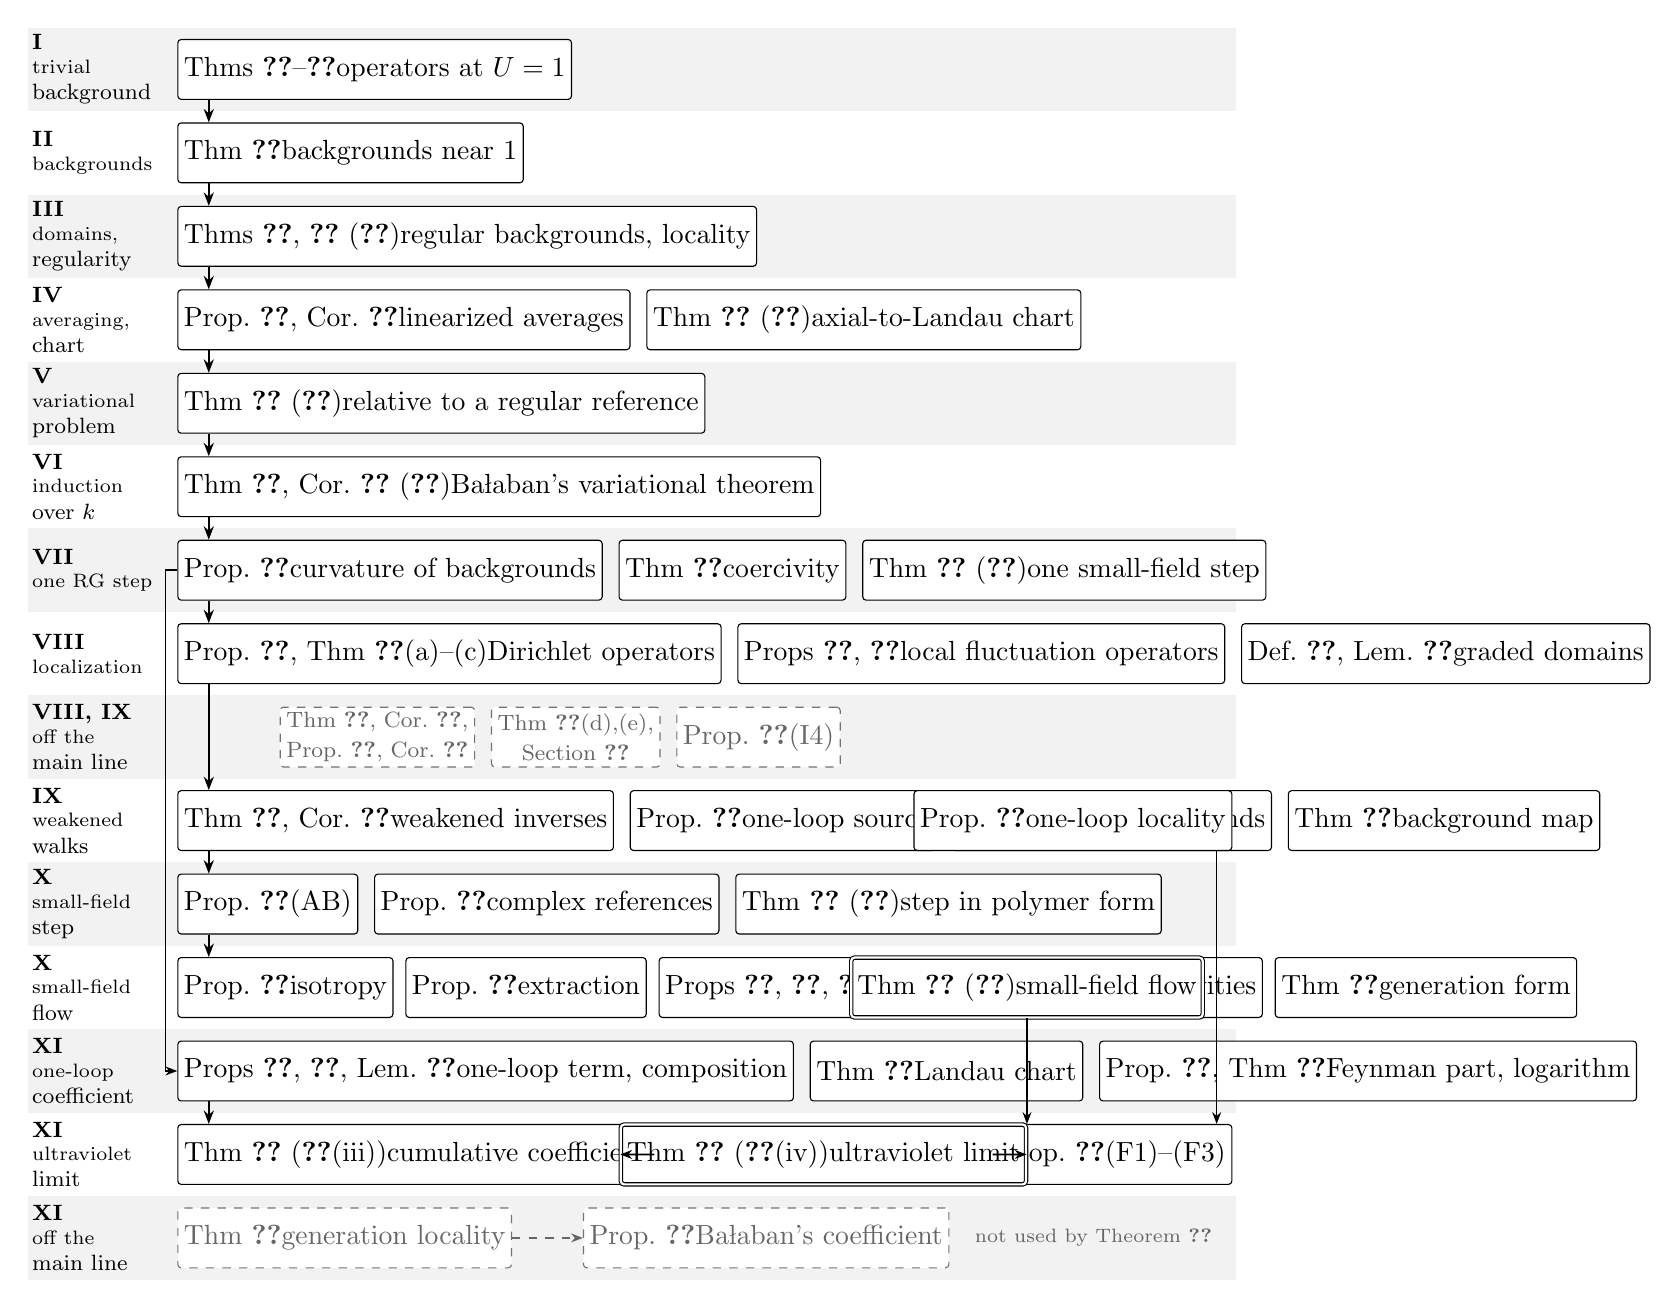
\begin{tikzpicture}[x=1cm,y=1cm,
  res/.style={draw,rounded corners=1.2pt,fill=white,align=flush center,inner xsep=2.2pt,inner ysep=1.5pt,minimum height=7.6mm},
  head/.style={res,double,double distance=0.8pt},
  off/.style={res,dashed,draw=black!55,text=black!60},
  plab/.style={anchor=west,align=flush left,inner sep=0pt,font=\footnotesize},
  spine/.style={-{Stealth[length=1.7mm]},thick},
  use/.style={-{Stealth[length=1.5mm]},semithick},
  ]
\def\h{1.06}\def\xo{1.9}
% bands
\foreach \i/\p/\s in {0/I/{trivial\\background},1/II/backgrounds,2/III/{domains,\\regularity},
  3/IV/{averaging,\\chart},4/V/{variational\\problem},5/VI/{induction\\over $k$},6/VII/{one RG step},
  7/VIII/localization,8/{VIII, IX}/{off the\\main line},9/IX/{weakened\\walks},10/X/{small-field\\step},
  11/X/{small-field\\flow},12/XI/{one-loop\\coefficient},13/XI/{ultraviolet\\limit},14/XI/{off the\\main line}}{
  \pgfmathsetmacro\yy{-\i*\h}
  \pgfmathparse{int(mod(\i,2))}
  \ifnum\pgfmathresult=0 \fill[black!5] (0,\yy-0.5*\h) rectangle (15.35,\yy+0.5*\h);\fi
  \node[plab] at (0.05,\yy) {\textbf{\p}\\[-1pt]\scriptsize\s};
}
% Parts I--VII
\node[res,anchor=west] (a0) at (\xo,0) {\GMr{Thms~\ref{thm:A}--\ref{thm:E}}{operators at $U=1$}};
\node[res,anchor=west] (a1) at (\xo,-\h) {\GMr{Thm~\ref{thm:F}}{backgrounds near $1$}};
\node[res,anchor=west] (a2) at (\xo,-2*\h) {\GMr{Thms~\ref{thm:reg-gauge}, \ref{thm:reg-locality} (\ref{thm:G})}{regular backgrounds, locality}};
\node[res,anchor=west] (a3) at (\xo,-3*\h) {\GMr{Prop.~\ref{prop:linearized-averages}, Cor.~\ref{cor:parts-apply}}{linearized averages}};
\node[res,right=2mm of a3] (b3) {\GMr{Thm~\ref{thm:chart} (\ref{thm:H})}{axial-to-Landau chart}};
\node[res,anchor=west] (a4) at (\xo,-4*\h) {\GMr{Thm~\ref{thm:variational} (\ref{thm:I})}{relative to a regular reference}};
\node[res,anchor=west] (a5) at (\xo,-5*\h) {\GMr{Thm~\ref{thm:balaban}, Cor.~\ref{cor:regularity} (\ref{thm:J})}{Ba\l aban's variational theorem}};
\node[res,anchor=west] (a6) at (\xo,-6*\h) {\GMr{Prop.~\ref{prop:sharp-curvature}}{curvature of backgrounds}};
\node[res,right=2mm of a6] (b6) {\GMr{Thm~\ref{thm:step-coercive}}{coercivity}};
\node[res,right=2mm of b6] (c6) {\GMr{Thm~\ref{thm:step} (\ref{thm:K})}{one small-field step}};
% Part VIII, and what Parts VIII and IX leave off the main line
\node[res,anchor=west] (a7) at (\xo,-7*\h) {\GMr{Prop.~\ref{prop:dirichlet-averaged}, Thm~\ref{thm:ID}(a)--(c)}{Dirichlet operators}};
\node[res,right=2mm of a7] (b7) {\GMr{Props~\ref{prop:dirichlet-hessian}, \ref{prop:local-fluct}}{local fluctuation operators}};
\node[res,right=2mm of b7] (c7) {\GMr{Def.~\ref{def:graded}, Lem.~\ref{lem:quadratic-bound}}{graded domains}};
\node[off,anchor=west] (b8) at (\xo+1.3,-8*\h) {\footnotesize Thm~\ref{thm:local-covariance}, Cor.~\ref{cor:large-changes},\\[-1pt]\footnotesize Prop.~\ref{prop:det-local}, Cor.~\ref{cor:one-loop}};
\node[off,right=2mm of b8] (c8) {\footnotesize Thm~\ref{thm:ID}(d),(e),\\[-1pt]\footnotesize Section~\ref{sec:interaction-local}};
\node[off,right=2mm of c8] (d8) {\GMr{Prop.~\ref{prop:schauder}}{(I4)}};
% Part IX
\node[res,anchor=west] (a9) at (\xo,-9*\h) {\GMr{Thm~\ref{thm:weak-inverse}, Cor.~\ref{cor:weak-covariance}}{weakened inverses}};
\node[res,right=2mm of a9] (b9) {\GMr{Prop.~\ref{prop:one-loop-polymer}}{one-loop source}};
\node[res,right=2mm of b9] (c9) {\GMr{Thm~\ref{thm:HC-pointwise}}{pointwise bounds}};
\node[res,right=2mm of c9] (d9) {\GMr{Thm~\ref{thm:weak-bg}}{background map}};
\node[res,anchor=east] (f9) at (15.3,-9*\h) {\GMr{Prop.~\ref{prop:one-loop-local}}{one-loop locality}};
% Part X
\node[res,anchor=west] (a10) at (\xo,-10*\h) {\GMr{Prop.~\ref{prop:AB}}{(AB)}};
\node[res,right=2mm of a10] (b10) {\GMr{Prop.~\ref{prop:complex-ext}}{complex references}};
\node[res,right=2mm of b10] (c10) {\GMr{Thm~\ref{thm:sf-step} (\ref{thm:L})}{step in polymer form}};
\node[res,anchor=west] (a11) at (\xo,-11*\h) {\GMr{Prop.~\ref{prop:period-iso}}{isotropy}};
\node[res,right=1.5mm of a11] (b11) {\GMr{Prop.~\ref{prop:extraction}}{extraction}};
\node[res,right=1.5mm of b11] (c11) {\GMr{Props~\ref{prop:first-step}, \ref{prop:vacuum}, \ref{prop:old-activities}}{first step, vacuum, old activities}};
\node[res,right=1.5mm of c11] (d11) {\GMr{Thm~\ref{thm:gen-step}}{generation form}};
\node[head,anchor=east] (e11) at (14.93,-11*\h) {\GMr{Thm~\ref{thm:sf-flow} (\ref{thm:N})}{small-field flow}};
% Part XI
\node[res,anchor=west] (a12) at (\xo,-12*\h) {\GMr{Props~\ref{prop:ol-laplace}, \ref{prop:ol-composition}, Lem.~\ref{lem:ol-symmetry}}{one-loop term, composition}};
\node[res,right=2mm of a12] (b12) {\GMr{Thm~\ref{thm:ol-chart}}{Landau chart}};
\node[res,right=2mm of b12] (c12) {\GMr{Prop.~\ref{prop:ol-reduction}, Thm~\ref{thm:ol-log}}{Feynman part, logarithm}};
\node[res,anchor=west] (a13) at (\xo,-13*\h) {\GMr{Thm~\ref{thm:ol-cumulative} (\ref{thm:M}(iii))}{cumulative coefficient}};
\node[res,anchor=east,minimum width=2.5cm] (c13) at (15.3,-13*\h) {\GMr{Prop.~\ref{prop:flow-F}}{(F1)--(F3)}};
\node[head] (b13) at ($(a13.east)!0.5!(c13.west)$) {\GMr{Thm~\ref{thm:ol-uv} (\ref{thm:M}(iv))}{ultraviolet limit}};
\node[off,anchor=west] (a14) at (\xo,-14*\h) {\GMr{Thm~\ref{thm:gen-locality}}{generation locality}};
\node[off,right=9mm of a14] (b14) {\GMr{Prop.~\ref{prop:beta-identification}}{Ba\l aban's coefficient}};
\node[anchor=west,font=\scriptsize,text=black!60] at ([xshift=2mm]b14.east) {not used by Theorem~\ref{thm:M}};
% arrows: the main line
\foreach \u/\v in {a0/a1,a1/a2,a2/a3,a3/a4,a4/a5,a5/a6,a6/a7,a7/a9,a9/a10,a10/a11,a12/a13}
  \draw[spine] ([xshift=4mm]\u.south west) -- ([xshift=4mm]\v.north west);
\draw[use] (a6.west) -- ++(-0.15,0) |- (a12.west);
\draw[use] (a13) -- (b13);
\draw[use] (c13) -- (b13);
\draw[use] (e11.south) -- (e11.south |- c13.north);
\draw[use] ([xshift=-2mm]f9.south east) -- ([xshift=-2mm]f9.south east |- c13.north);
\draw[use,dashed,draw=black!60] (a14) -- (b14);
\end{tikzpicture}
\caption{The main line of the proof. Each band is a Part; Part~X is split into the step (Sections~\ref{sec:complex-references}--\ref{sec:cluster}) and the flow (Sections~\ref{sec:flow}--\ref{sec:flow4}), and Part~XI into Sections~\ref{sec:ol-composite}--\ref{sec:ol-feynman}, Section~\ref{sec:ol-uv} and Section~\ref{sec:gen-locality}. A box names results by their printed numbers; the letter in parentheses is the theorem of Section~\ref{sec:intro} that collects them. A thick arrow: the next band of the main line uses the band above it. The thin arrow on the left: Sections~\ref{sec:ol-composite}--\ref{sec:ol-feynman} use Parts~I--VII and, from Part~X, mainly Propositions~\ref{prop:jacobians}, \ref{prop:first-step} and Lemma~\ref{lem:first-step-formula}. The thin arrows on the right: Proposition~\ref{prop:flow-F}, the properties (F1)--(F3), uses the flow and the torus independence of the one-loop pieces (the reading guide in Section~\ref{sec:intro}). Double frames: Theorem~\ref{thm:sf-flow}, the small-field flow (Theorem~\ref{thm:N}), and Theorem~\ref{thm:ol-uv}, the ultraviolet limit (Theorem~\ref{thm:M}(iv)). Grey dashed frames: results off the main line. These are the radius-type results of Part~VIII, superseded by Parts~IX and~X (the status paragraphs of Sections~\ref{sec:localization}--\ref{sec:interaction-local}); Theorem~\ref{thm:ID}(d),(e), used only in Section~\ref{sec:interaction-local}; Proposition~\ref{prop:schauder}, not used outside Section~\ref{sec:interior-lp}; and Theorem~\ref{thm:gen-locality}, which gives Proposition~\ref{prop:beta-identification}. Theorem~\ref{thm:M} does not use Proposition~\ref{prop:beta-identification}.}
\label{fig:G-mainline}
\end{gfigure}


The note has eleven Parts. Table~\ref{tab:G-parts} lists their main results, and Figure~\ref{fig:G-mainline} shows how these results feed Theorems~\ref{thm:N} and~\ref{thm:M}(iv). The main theorems of Section~\ref{sec:intro} are attached to the Parts: Theorems~\ref{thm:A}--\ref{thm:E} to Part~I, \ref{thm:F} to Part~II, \ref{thm:G} to Part~III, \ref{thm:H} to Part~IV, \ref{thm:I} to Part~V, \ref{thm:J} to Part~VI, \ref{thm:K} to Part~VII, \ref{thm:L} and~\ref{thm:N} to Part~X, and \ref{thm:M} to Part~XI. The introduction of each Part lists what it imports and what it exports.

\begin{table}[tbp]
\centering\small
\renewcommand{\arraystretch}{1.15}
\begin{tabular}{|p{0.13\textwidth}|p{0.57\textwidth}|p{0.19\textwidth}|}
\hline
Part & Main results & On the main line\tabularnewline
\hline
I, \S\S\ref{sec:setup}--\ref{sec:gauge-min} & \raggedright Theorems~\ref{thm:A}--\ref{thm:E}: at $U=1$, coercivity (Theorem~\ref{thm:gauge-coercive}), decay and $C^{1,\alpha}$ bounds for the Green functions and the minimizer maps, and decay, $C^1$ and $C^{0,\alpha}$ bounds for the constrained Green function $\bC$ (Theorems~\ref{thm:scalar-green}, \ref{thm:gauge-green}, \ref{thm:H-gauge}, \ref{thm:C-gauge}); interior regularity (Theorem~\ref{thm:local-regularity}) & \raggedright yes; Part~XI uses it in infinite volume (Corollary~\ref{cor:ol-part-one})\tabularnewline
II, \S\S\ref{sec:background}--\ref{sec:cov-min} & \raggedright Theorem~\ref{thm:F}: the same operators at complex backgrounds close to $1$ in a global gauge (Theorems~\ref{thm:cov-scalar}, \ref{thm:cov-gauge}, \ref{thm:cov-min}) & yes\tabularnewline
III, \S\S\ref{sec:domains}--\ref{sec:random-walk} & \raggedright Theorem~\ref{thm:G}: Dirichlet operators and coercivity at $(M,\eps)$-regular backgrounds (Theorem~\ref{thm:reg-coercive}), decay (Theorems~\ref{thm:reg-gauge}, \ref{thm:reg-min}), locality (Theorem~\ref{thm:reg-locality}), the scalar random walk (Theorem~\ref{thm:random-walk}) & yes\tabularnewline
IV, \S\S\ref{sec:averaging}--\ref{sec:chart} & \raggedright Theorem~\ref{thm:H}: Ba\l aban's symmetric averaging; its linearized gauge-adapted form is an averaging pair with $E=0$ (Proposition~\ref{prop:linearized-averages}, Corollary~\ref{cor:parts-apply}); the axial-to-Landau chart (Theorem~\ref{thm:chart}) & yes\tabularnewline
V, \S\S\ref{sec:var-theorem}--\ref{sec:var-regularity} & \raggedright Theorem~\ref{thm:I}: the variational problem relative to a regular reference (Theorem~\ref{thm:variational}) & yes\tabularnewline
VI, \S\S\ref{sec:local-gauges}--\ref{sec:induction} & \raggedright Theorem~\ref{thm:J}: the background field $U_k(V)$ for every $k$ (Theorem~\ref{thm:balaban}); regularity from gauge-invariant conditions (Corollary~\ref{cor:regularity}) & yes\tabularnewline
VII, \S\S\ref{sec:rg-step}--\ref{sec:covariance} & \raggedright Theorem~\ref{thm:K}: one step as a Gaussian integral (Theorem~\ref{thm:step}), coercivity (Theorem~\ref{thm:step-coercive}), the curvature of background fields (Proposition~\ref{prop:sharp-curvature}), lattice symmetry (Proposition~\ref{prop:symmetry}) & yes\tabularnewline
VIII, \S\S\ref{sec:dirichlet-averaged}--\ref{sec:interaction-local} & \raggedright Dirichlet averaged operators (Proposition~\ref{prop:dirichlet-averaged}), interior bounds (Theorem~\ref{thm:ID}), Dirichlet Hessians and local fluctuation operators (Propositions~\ref{prop:dirichlet-hessian}, \ref{prop:local-fluct}), graded domains (Definition~\ref{def:graded}), the quadratic bound (Lemma~\ref{lem:quadratic-bound}) & \raggedright partly: Theorem~\ref{thm:local-covariance}, Corollary~\ref{cor:large-changes}, Proposition~\ref{prop:det-local}, Corollary~\ref{cor:one-loop} and Section~\ref{sec:interaction-local} are superseded\tabularnewline
IX, \S\S\ref{sec:weakenable}--\ref{sec:weak-background} & \raggedright weakened inverses (Theorem~\ref{thm:weak-inverse}, Corollary~\ref{cor:weak-covariance}), the one-loop source in polymer form (Proposition~\ref{prop:one-loop-polymer}), torus independence (Proposition~\ref{prop:one-loop-local}), pointwise bounds by tiers (Theorems~\ref{thm:tier-walk}, \ref{thm:HC-pointwise}), the weakened background map (Theorem~\ref{thm:weak-bg}) & \raggedright yes; Proposition~\ref{prop:one-loop-local} serves Part~XI\tabularnewline
X, \S\S\ref{sec:complex-references}--\ref{sec:flow4} & \raggedright complex references (Propositions~\ref{prop:AB}, \ref{prop:complex-ext}); Theorem~\ref{thm:L}: the step in polymer form (Theorem~\ref{thm:sf-step}); generations and extraction (Propositions~\ref{prop:period-iso}, \ref{prop:extraction}); Theorem~\ref{thm:N}: the flow (Theorem~\ref{thm:sf-flow}, Corollary~\ref{cor:sf-stability}) & yes\tabularnewline
XI, \S\S\ref{sec:ol-composite}--\ref{sec:gen-locality} & \raggedright Theorem~\ref{thm:M}: composition and symmetry of the one-loop terms (Proposition~\ref{prop:ol-composition}, Lemma~\ref{lem:ol-symmetry}), the Landau-chart formula (Theorem~\ref{thm:ol-chart}), the logarithm (Theorem~\ref{thm:ol-log}), the cumulative coefficient (Theorem~\ref{thm:ol-cumulative}), (F1)--(F3) (Proposition~\ref{prop:flow-F}), the ultraviolet limit (Theorem~\ref{thm:ol-uv}) & \raggedright yes, up to Theorem~\ref{thm:ol-uv}; Section~\ref{sec:gen-locality} and Proposition~\ref{prop:beta-identification} are off it\tabularnewline
\hline
\end{tabular}
\caption{The Parts of the note and their main results. ``On the main line'' refers to the line that ends at Theorems~\ref{thm:sf-flow} and~\ref{thm:ol-uv}, as in the reading guide of Section~\ref{sec:intro}.}\label{tab:G-parts}
\end{table}

\paragraph{Four reading paths.}
\begin{enumerate}[label=(\alph*)]
\item \emph{An overview in one day.} The statements of Theorems~\ref{thm:A}--\ref{thm:N}; Sections~\ref{g:read}--\ref{g:strategy} of this guide; the introductions of the Parts; and the remarks that explain the flow: Remarks~\ref{rem:flow-status}, \ref{rem:parameters}, \ref{rem:sf-reference}, \ref{rem:flow-constants} and~\ref{rem:sf-flow}.
\item \emph{The main line to Theorem~\ref{thm:N}.} Parts~I--VII. From Part~VIII: Section~\ref{sec:dirichlet-averaged}, the interior estimates of Section~\ref{sec:interior}, Section~\ref{sec:localization} up to Proposition~\ref{prop:local-fluct}, and Section~\ref{sec:det-local} except Proposition~\ref{prop:det-local} and Corollary~\ref{cor:one-loop}. Then Parts~IX and~X. The radius-type results of Part~VIII, Theorem~\ref{thm:local-covariance}, Corollary~\ref{cor:large-changes}, Proposition~\ref{prop:det-local}, Corollary~\ref{cor:one-loop} and Section~\ref{sec:interaction-local}, are replaced on this line by Parts~IX and~X, and each is marked where it appears (the reading guide of Section~\ref{sec:intro}).
\item \emph{The one-loop line to Theorem~\ref{thm:M}(iv).} Sections~\ref{sec:ol-composite}--\ref{sec:ol-feynman} use Parts~I--VII and, from Part~X, mainly Propositions~\ref{prop:jacobians} and~\ref{prop:first-step} and Lemma~\ref{lem:first-step-formula}. Section~\ref{sec:ol-uv} combines them with the flow; it uses Part~X throughout and the torus independence of Section~\ref{subsec:torus-independence}. Section~\ref{sec:gen-locality} and Proposition~\ref{prop:beta-identification} are not used by Theorem~\ref{thm:ol-uv} (Remark~\ref{rem:ol-remains}(c)).
\item \emph{The operator theory alone.} Parts~I--III, with Theorems~\ref{thm:A}--\ref{thm:G}. Part~I is self-contained; for the Green function of the fine lattice it uses Appendix~\ref{app:green} (Section~\ref{sec:regularity}). The gauge-field random walk of Theorem~\ref{thm:G}(iv) is completed in Section~\ref{sec:nested-walks} of Part~IX.
\end{enumerate}

\paragraph{The companion.} The companion volume \emph{Details} works out the steps of the proofs of Parts~VII--XI, and its chapter on the parameter ledger records the constants of these Parts with their dependencies and the order in which they are chosen. Its chapters follow the Parts: Part~VII, Part~VIII, Part~IX, the two halves of Part~X and the two halves of Part~XI. A proof of this note that the companion expands carries the marginal link \textsf{Details}. The link opens the companion at the first Detail on that result; conversely, the companion's references to the note are links into this file. Both kinds of link are relative. They work when the note, \texttt{YM4-small-field-flow.pdf}, and the companion, \texttt{Details/details.pdf}, keep their relative places, and they break if the two files are separated. Acrobat, Skim, Okular and Evince follow links to a named place in another file; macOS Preview follows them poorly. The companion's index of the note's results serves when a link does not work.

\paragraph{Where in the note.} The reading guide in Section~\ref{sec:intro}; the status paragraphs at the head of Sections~\ref{sec:localization}--\ref{sec:interaction-local}.

\paragraph{In the companion.} The chapter ``How to read this volume'', and the index.

\gsection{The result}\label{g:result}

\paragraph{The lattice model.} The gauge group $G$ is compact and connected, and $d=4$ (Section~\ref{sec:intro}). The torus has physical side $\ell$; its finest lattice $\T^{(0)}$ has spacing $\epsilon=L^{-N}$, with the odd block factor $L\ge3$ and the number $N$ of scales (Section~\ref{subsec:tf-scales}). The Wilson action of a configuration $U$ is
\[
S(U)=\sum_p\Big(\mathsf N-\tfrac12\operatorname{tr}\big(U(\partial p)+U(\partial p)^{-1}\big)\Big),
\]
summed over the positively oriented plaquettes, with no power of the spacing in front, since in four dimensions the action is dimensionless (Section~\ref{sec:action}). The trace is that of a representation $\rho$ by $\mathsf N\times\mathsf N$ matrices, with $\operatorname{tr}_\rho(T^aT^b)=T_\rho\delta^{ab}$ for Hermitian generators $T^a$ (Section~\ref{sec:ol-feynman}). The lattice measure is $\rho_0(V)\prod_bdV(b)$ on $\T^{(0)}$, with the Haar measure on each positively oriented bond, $\rho_0=\exp(-g_0^{-2}S-E_0)$, the bare coupling $g_0$ and a constant $E_0$ (Theorem~\ref{thm:N}).

\paragraph{Normalization of the coupling.} The period density of $S$, its second-order part per unit volume at the linear field of constant curvature $F=F^aT^a$, is $\frac12\sum_{\mu<\nu}\operatorname{tr}(F_{\mu\nu}^2)=\frac12T_\rho\sum_{\mu<\nu}F^a_{\mu\nu}F^a_{\mu\nu}$ (Theorem~\ref{thm:sf-flow}(c)). So $g^{-2}S$ has the period density of the continuum action $\frac1{2g_{\rm std}^2}\sum_{\mu<\nu}\int F^a_{\mu\nu}F^a_{\mu\nu}$ with $g_{\rm std}^2=g^2/T_\rho$; for $SU(\mathsf N)$ in the fundamental representation $T_\rho=\frac12$ and $g_{\rm std}^2=2g^2$ (Lemma~\ref{lem:ol-classical}; Section~\ref{sec:ol-feynman}, the paragraph ``Normalization of the coupling''). The one-loop coefficient per step is $\beta_\infty=\frac{11C_A}{24\pi^2T_\rho}\log L$ for $g^{-2}$, i.e.\ $\frac{11C_A}{24\pi^2}\log L$ for $g_{\rm std}^{-2}$, and $\beta_\infty=\frac{11\mathsf N}{12\pi^2}\log L$ for $SU(\mathsf N)$ in the fundamental representation (Theorem~\ref{thm:ol-log}). Its sign is that of asymptotic freedom (proof of Lemma~\ref{lem:ol-classical}), and its value agrees with the heat-kernel coefficient of the continuum one-loop term (Remark~\ref{rem:ol-heat-kernel}).

\paragraph{The gauge group, Part by Part.} The hypotheses on $G$ grow along the note (Section~\ref{sec:intro}).
\begin{itemize}
\item \emph{Parts~I--VI:} $G$ compact and connected.
\item \emph{Parts~VII--X:} $G$ also semisimple; Part~VII does not use it (Section~\ref{sec:rg-step}). An $\operatorname{Ad}(G)$-invariant vector of $\mathfrak g^c$ then vanishes, so a normalized, gauge-invariant activity has no term of first order and is of second order in the curvature, the current and the complex part (Lemma~\ref{lem:quadratic-bound} and its proof). This makes the one-loop source marginal rather than relevant (Remark~\ref{rem:one-loop-polymer}(b)), and it is why groups with abelian factors are not treated.
\item \emph{The flow (Sections~\ref{sec:generations}--\ref{sec:flow4}) and Part~XI:} $G$ simple. A quadratic form in a constant curvature that is invariant under conjugation by $G$ and under $B_4$ is then a single multiple of the isotropic form (Lemma~\ref{lem:b4-forms}(a)). So the period density of a generation is $\beta_E$ times that of $S$ (Proposition~\ref{prop:period-iso}), and the running coupling is one number. Part~XI uses the same fact in \eqref{eq:ol-kappa}.
\end{itemize}

\paragraph{The step and the small-field model.} The renormalization group map $T$ sends a density of the configurations $V$ on $\T=\T^{(k)}$ to the image density of $V'$ on $\T'=\T^{(k+1)}$ under Ba\l aban's one-step averaging $\mathfrak a'$ \eqref{eq:rg-map}. The note iterates the \emph{small-field step} $T_{\rm sf}(\rho)=T^{\rm gf}(\chi^{\rm w}\chi_\xi\,\rho)$ (Definition~\ref{def:small-field-step}). Here $T^{\rm gf}$ is $T$ with Ba\l aban's exponential gauge-fixing function $\mathrm{gf}_W$ (Definition~\ref{def:gf-step}); on the coarse configurations of Lemma~\ref{lem:composition} it agrees with $T$ on integrands that are invariant under the gauge transformations $\mathcal G'$ of the blocks and vanish outside Ba\l aban's regular set $\mathfrak M$ (Lemma~\ref{lem:gf-step-invariance}(iv)). The functions $\chi^{\rm w}$, $\chi_\xi$ are the cutoffs of Table~\ref{tab:G-cutoffs}. The densities of the small-field model are $\rho_{k+1}=\one_{\mathfrak U_{k+1}(h_{k+1})}T_{\rm sf}(\rho_k)$ (Remark~\ref{rem:sf-reference}(c), Theorem~\ref{thm:N}). The threshold $h_k$ and the bound $w$ tend to $0$ with the coupling, while $p_0$ grows; so the small-field domain shrinks with the coupling, unlike Ba\l aban's (Remark~\ref{rem:sf-flow}(a)).

\begin{table}[tbp]
\centering\small
\renewcommand{\arraystretch}{1.12}
\begin{tabular}{|p{0.19\textwidth}|p{0.31\textwidth}|p{0.17\textwidth}|p{0.19\textwidth}|}
\hline
Cutoff & Condition & Size & Defined at\tabularnewline
\hline
\raggedright small-field set $\mathfrak U_k(h_k)$ & \raggedright the curvature of $V$ on $\T^{(k)}$ is at most $h_k$ at every plaquette & \raggedright $h_k=p(g_k)\,g_k$ & \raggedright Definition~\ref{def:curvature}, Section~\ref{subsec:flow-parameters}\tabularnewline
\raggedright fluctuation cutoff $\chi^{\rm w}$ & \raggedright $V(b)=e^{\ii Z(b)}W(b)$ with $|Z(b)|\le w$ on every bond, $W$ the base of the step & \raggedright $w=C_wL^dC_T\,g\,p_0(g)$ & \raggedright Definition~\ref{def:chi-w}, Remark~\ref{rem:flow-constants}(iii)\tabularnewline
\raggedright white-noise cutoff $\chi_\xi$ & \raggedright $|\xi(b)|\le p_0$ on the bonds of $\mathfrak F$, where $Z=g\,C_k^{1/2}\xi$ on $\mathfrak F$ & \raggedright $p_0=p_0(g)$ & \raggedright Definition~\ref{def:small-field-step}, Section~\ref{subsec:flow-parameters}\tabularnewline
\hline
\end{tabular}
\caption{The cutoffs of the step from scale $k$ to scale $k+1$, at $g=g_k$. The functions $p$, $p_0$ grow more slowly than every power of $g^{-1}$, and $p_0/p\to0$ as $g\to0$, for instance $p_0=(\log g^{-1})^q$, $p=(\log g^{-1})^{q'}$, $0<q<q'$ (Section~\ref{subsec:flow-parameters}); for $\gamma$ small, ($\Gamma$2) gives $8C_wL^dC_Tp_0\le p$, hence $4w\le\frac12h_k$ (Remark~\ref{rem:flow-constants}, Consequences). The cutoffs $\chi^{\rm w}$ and $\chi_\xi$ are not invariant under $\mathcal G'$ (Remark~\ref{rem:sf-reference}(c)).}\label{tab:G-cutoffs}
\end{table}

\paragraph{The model as one integral.} With $V_0=V$, $V_{k+1}=\mathfrak a_{k+1}(V_k)$ and $W_k$ the base of $V_{k+1}$, the small-field model unrolls to one integral over the configurations of scale~$0$ (Remark~\ref{rem:sf-reference}(c)):
\[
\int\rho_K\,dV_K=\int\prod_bdV(b)\ \rho_0(V)\prod_{k<K}\Big[\mathrm{gf}_{W_k}(V_k)\,\chi^{\rm w}_k(V_k)\,\chi_{\xi,k}(V_k)\,\one_{\mathfrak U_{k+1}(h_{k+1})}(V_{k+1})\Big].
\]
The cutoffs of step $k$ depend on $V_{k+1}$ as well as on $V_k$, and they are not invariant under $\mathcal G'$, so the small-field steps define a modified model. What a step discards is nonnegative (Lemma~\ref{lem:gf-step-invariance}(iv)); hence the partition function of the small-field model is at most that of the lattice theory with the same counterterm, $Z_{\rm sf}=\int\rho_K\le\int\rho_0=Z_{\rm lat}$ (Remark~\ref{rem:sf-reference}(c)).

\paragraph{The flow in words: Theorem~\ref{thm:N}.} Theorem~\ref{thm:N} summarizes Theorem~\ref{thm:sf-flow}, Propositions~\ref{prop:period-iso}, \ref{prop:extraction}, \ref{prop:flow-continuity} and Corollaries~\ref{cor:bare-continuity}, \ref{cor:sf-stability}. Hypotheses: $G$ simple; the parameters as in Remark~\ref{rem:parameters} (Section~\ref{g:parameters}); $\gamma$ subject to ($\Gamma$1)--($\Gamma$3) of Remark~\ref{rem:flow-constants}; the last torus of side $n_K\ge n_{\min}$, with $\ell L^N$ a power of $L$ (Section~\ref{g:scales}); $g_0\in(0,\gamma]$. Then, at every scale $k$ such that $g_1,\dots,g_k\le\gamma$:
\begin{itemize}
\item on the small-field set, $\rho_k(V)=\mathcal Z_k\exp\big(-g_k^{-2}S(U_k)-\eps_k|\T^{(k)}|+\sum_{j\le k}(E^{(j)}-\beta_jS)(U_k)\big)$ at the background field $U_k=U_k(V)$: Ba\l aban's generation form (Theorem~\ref{thm:N}(i));
\item each generation $E^{(j)}$ is bounded once, at its creation scale, by $\mathsf Ke^{-\kappa_nd_j(X)}$ on domains whose constants do not depend on the coupling, with the rate $\kappa_n$ of Remark~\ref{rem:parameters}(1) and the tree length $d_j(X)$ of the polymer $X$ (Section~\ref{subsec:flow-norm}; Theorem~\ref{thm:N}(ii));
\item $\beta_j$ is read off from the period density of $E^{(j)}$, which is exactly isotropic; $|\beta_j|\le C_\beta\mathsf K$, $g_j^{-2}=g_{j-1}^{-2}-\beta_j$ and $\frac34g_{j-1}\le g_j\le2g_{j-1}$ (Theorem~\ref{thm:N}(iii), (v));
\item at a later scale $j+m$, the small polymers of $E^{(j)}$ in a grid cube $\Box$ add up to $\beta_jS_\Box$ up to $C\mathsf KL^{-\alpha m}$ for $m\ge m_0$, the age from which the small polymers are extracted (Definition~\ref{def:polymer-classes}), and the other polymers carry a factor $L^{-m}$ (Theorem~\ref{thm:N}(iv));
\item every step satisfies the hypotheses of Theorem~\ref{thm:L} (Theorem~\ref{thm:N}(v)), and the generations and coefficients depend continuously on the couplings (Theorem~\ref{thm:N}(vii)).
\end{itemize}
The constants depend only on the parameters fixed before $\gamma$ (one also on $p_0$), not on $k$, $K$, the torus or the couplings (Theorem~\ref{thm:N}). No behaviour of the couplings beyond $g_k\le\gamma$ is assumed (Remark~\ref{rem:sf-flow}(a)).

\paragraph{What Theorem~\ref{thm:N}(vi) says.} Let $g_1,\dots,g_K\le\gamma$, and fix the counterterm $E_0$ by $\eps_K=0$; exactly one $E_0$ does this. The partition function of the small-field model is then $\mathcal Z_KI_K$, with an explicit product $\mathcal Z_K$ of normalizations and $e^{-c|\T^{(K)}|}\le I_K\le e^{c|\T^{(K)}|}$, where $c$ depends on the last coupling $g_K$ and on the parameters, not on $N$, $K$, the torus or $g_0,\dots,g_{K-1}$ (Corollary~\ref{cor:sf-stability}). So, at a fixed last coupling, $I_K=e^{O(|\T^{(K)}|)}$ uniformly in the number of steps, with $|\T^{(K)}|=n_K^4$ the volume in the units of the last scale. The bound is crude, per unit volume, which suffices because the final torus is fixed (Remark~\ref{rem:sf-reference}(a)); $\mathcal Z_K$ is not compared with the normalizations of a Gaussian reference (Remark~\ref{rem:sf-reference}(b)).

\paragraph{The ultraviolet limit in words: Theorem~\ref{thm:M}(iv).} This is Theorem~\ref{thm:ol-uv}. Let $G$ be simple, the parameters and the torus as in Theorem~\ref{thm:N}, $p_0(g)=(\log g^{-1})^q$, and $\gamma$ subject to ($\Gamma$1)--($\Gamma$4) and the two further conditions of Theorem~\ref{thm:ol-uv}. There are $g_{\rm uv}>0$ and $C$, independent of $K$ and of the torus, such that for $0<g\le g_{\rm uv}$ and every $K$ some bare coupling $g_0$, depending on $K$, $g$ and the torus, gives a flow in $(0,\gamma]$ with $g_K=g$ and
\[
\Big|\frac1{g_k^2}-\frac1{g^2}-(K-k)\beta_\infty\Big|\le C\big(\log(K-k+2)\big)^{6q+1}\qquad(k\le K).
\]
At $k=0$: $g_0^{-2}=g^{-2}+K\beta_\infty$ up to a power of $\log(K+2)$, so the bare coupling tends to $0$ as the number of steps grows. With $K=N$ the last lattice is the unit lattice of the torus of physical side $\ell$, so $n_K=\ell$ and the torus conditions read $\ell\ge n_{\min}$, $\ell$ a power of $L$; letting $N\to\infty$ at fixed $\ell$ shrinks $\epsilon=L^{-N}$, and the bound is uniform in $N$ (Section~\ref{subsec:tf-scales}). The theorem concerns the couplings of the small-field model (Remark~\ref{rem:ol-remains}(a)). Theorem~\ref{thm:M}(i)--(iii) compute $\beta_\infty$ (Section~\ref{g:oneloop}).

\paragraph{No step of the main line is conditional.} The hypotheses of Theorems~\ref{thm:K} and~\ref{thm:L} on the density, the coupling and the old activities hold at every step of the flow (Theorem~\ref{thm:gen-step}(a), Theorem~\ref{thm:sf-flow}(e)). The hypothesis $g_k\le\gamma$ of Theorem~\ref{thm:N} holds, up to the last scale, for the bare coupling of Theorem~\ref{thm:ol-uv}. The properties (F1)--(F3) that Theorem~\ref{thm:ol-uv} uses are proved in Proposition~\ref{prop:flow-F}. Proposition~\ref{prop:beta-identification} is proved without a rate, and Theorem~\ref{thm:ol-uv} does not use it (Remark~\ref{rem:ol-remains}(c)).

\paragraph{What is not proved.} The large-field stage and the removal of the small-field modification (Remark~\ref{rem:sf-reference}(d)), hence any statement on the partition function or the correlation functions of the lattice theory itself (Section~\ref{sec:intro}, ``What is not done here''). Any limit of the measure or of correlation functions as $\epsilon\to0$: Theorem~\ref{thm:ol-uv} concerns the couplings only. The exact lower half of the analogue of Ba\l aban's (0.31) for the last $m_1$ steps (Remark~\ref{rem:ol-remains}(c)). A rate, or uniformity in the couplings, in Proposition~\ref{prop:beta-identification} (Remark~\ref{rem:gl-rate}). Smoothness in the couplings; only continuity is proved (Proposition~\ref{prop:flow-continuity}). Bounds linear in the size for gauges on cubes of size $c\,\eps_1^{-1}$; the bounds are polynomial (Remark~\ref{rem:large-cubes}). Gauge groups with abelian factors, and dimensions other than $4$ (Section~\ref{sec:intro}).

\paragraph{Ba\l aban's theorems.} Four of the theorems that the note cites by number concern the variational problem and the flow.
\begin{itemize}
\item \cite[Theorem~1]{BalVar}, the variational theorem: Theorem~\ref{thm:I} is its content for one step, given a reference, and Theorem~\ref{thm:J} its version on the torus for every $k$, without nested domains (Section~\ref{sec:intro}, after Theorems~\ref{thm:I} and~\ref{thm:J}).
\item \cite[Theorem~1]{BalYM4I} asserts the generation form (0.22)--(0.24) with terms that satisfy the later-scale bounds (0.29). \cite[Theorem~3]{BalYM4I} is the inductive statement of the flow under $0<g_k\le\gamma$; Theorem~\ref{thm:sf-flow} is its analogue for the small-field model on the torus (Remark~\ref{rem:sf-flow}(a)).
\item \cite[Theorem~2]{BalYM4I}, stated for $SU(2)$, gives a bare coupling with $\frac1{g^2}+\beta\log(L^k\varepsilon)^{-1}\le\frac1{g_k^2}\le\frac1{g^2}+\beta'\log(L^k\varepsilon)^{-1}$, $0<\beta\le\beta'$: his (0.31), where $\log(L^k\varepsilon)^{-1}=(K-k)\log L$ for $\varepsilon=L^{-K}$. Theorem~\ref{thm:ol-uv} gives the analogue for the couplings of the small-field flow when $K-k\ge m_1$, and its upper half for all $k$. Ba\l aban's couplings come from his own generations, a different construction (Proposition~\ref{prop:beta-identification}(b); Section~\ref{sec:intro}, after Theorem~\ref{thm:M}).
\end{itemize}

\paragraph{Where in the note.} Section~\ref{sec:intro}; Remarks~\ref{rem:sf-reference}, \ref{rem:sf-flow} and~\ref{rem:ol-remains}; Theorems~\ref{thm:sf-flow} and~\ref{thm:ol-uv}, Corollary~\ref{cor:sf-stability}.

\paragraph{In the companion.} The chapters on the second halves of Parts~X and~XI.

\gsection{Scales, units and where the fields live}\label{g:scales}

% Figure of the guide (G2): the tower of lattices in the units of step k. Owner: WP7.
\begin{gfigure}[tp]
\centering
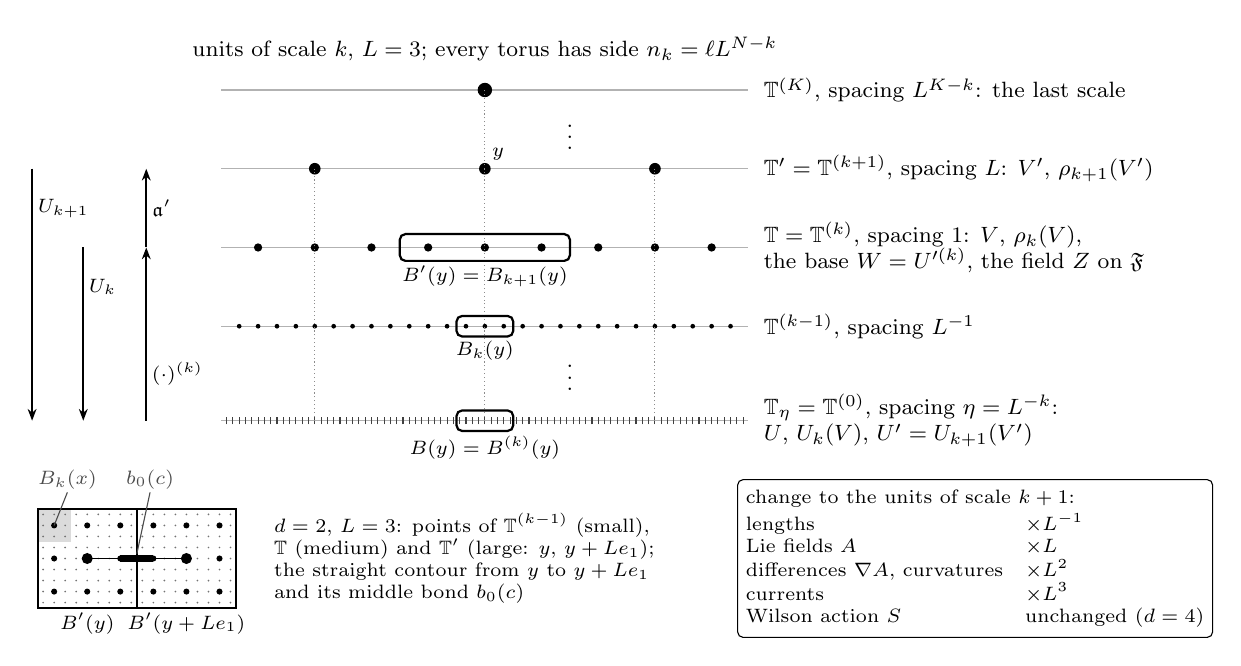
\begin{tikzpicture}[x=1cm,y=1cm,
  lev/.style={anchor=west,align=flush left,font=\footnotesize,inner sep=1pt},
  ar/.style={-{Stealth[length=1.5mm]},semithick},
  alab/.style={anchor=west,inner sep=1pt,font=\scriptsize},
  blk/.style={draw,rounded corners=2pt,thick},
  ]
\def\u{0.72}\def\X{6.05}
\def\yK{4.45}\def\yA{3.45}\def\yB{2.45}\def\yC{1.45}\def\yO{0.25}
% the levels
\foreach \yy in {\yK,\yA,\yB,\yC,\yO} \draw[black!30] (\X-4.65*\u,\yy) -- (\X+4.65*\u,\yy);
\foreach \i in {-41,...,41} \draw[black!75] (\X+\i*\u/9,\yO-0.045) -- (\X+\i*\u/9,\yO+0.045);
\foreach \i in {-13,...,13} \fill (\X+\i*\u/3,\yC) circle (0.85pt);
\foreach \i in {-4,...,4} \fill (\X+\i*\u,\yB) circle (1.5pt);
\foreach \i in {-1,0,1} \fill (\X+3*\i*\u,\yA) circle (2.1pt);
\fill (\X,\yK) circle (2.6pt);
\foreach \i in {-1,0,1} \draw[densely dotted,black!45] (\X+3*\i*\u,\yO) -- (\X+3*\i*\u,\yA);
\draw[densely dotted,black!45] (\X,\yA) -- (\X,\yK);
\node[font=\footnotesize] at (\X+1.5*\u,0.5*\yA+0.5*\yK) {$\vdots$};
\node[font=\footnotesize] at (\X+1.5*\u,0.5*\yC+0.5*\yO+0.05) {$\vdots$};
\node[font=\scriptsize,anchor=south west,inner sep=1pt] at (\X+0.05,\yA+0.06) {$y$};
% centred blocks around y
\draw[blk] (\X-1.5*\u,\yB-0.17) rectangle (\X+1.5*\u,\yB+0.17);
\node[font=\scriptsize,anchor=north,inner sep=1pt] at (\X,\yB-0.19) {$B'(y)=B_{k+1}(y)$};
\draw[blk] (\X-0.5*\u,\yC-0.13) rectangle (\X+0.5*\u,\yC+0.13);
\node[font=\scriptsize,anchor=north,inner sep=1pt] at (\X,\yC-0.15) {$B_k(y)$};
\draw[blk] (\X-0.5*\u,\yO-0.13) rectangle (\X+0.5*\u,\yO+0.13);
\node[font=\scriptsize,anchor=north,inner sep=1pt] at (\X,\yO-0.15) {$B(y)=B^{(k)}(y)$};
% maps between the levels
\draw[ar] (0.3,\yA) -- (0.3,\yO); \node[alab] at (0.33,0.5*\yA+0.5*\yB) {$U_{k+1}$};
\draw[ar] (0.95,\yB) -- (0.95,\yO); \node[alab] at (0.98,0.5*\yC+0.5*\yB) {$U_k$};
\draw[ar] (1.75,\yO) -- (1.75,\yB); \node[alab] at (1.78,0.5*\yC+0.5*\yO) {$(\cdot)^{(k)}$};
\draw[ar] (1.75,\yB) -- (1.75,\yA); \node[alab] at (1.78,0.5*\yB+0.5*\yA) {$\mathfrak a'$};
% what lives where
\node[lev] at (9.55,\yK) {$\T^{(K)}$, spacing $L^{K-k}$: the last scale};
\node[lev] at (9.55,\yA) {$\T'=\T^{(k+1)}$, spacing $L$: $V'$, $\rho_{k+1}(V')$};
\node[lev,text width=5.6cm] at (9.55,\yB) {$\T=\T^{(k)}$, spacing $1$: $V$, $\rho_k(V)$,\\ the base $W=U'^{(k)}$, the field $Z$ on $\mathfrak F$};
\node[lev] at (9.55,\yC) {$\T^{(k-1)}$, spacing $L^{-1}$};
\node[lev,text width=5.6cm] at (9.55,\yO) {$\Tf=\T^{(0)}$, spacing $\eta=L^{-k}$:\\ $U$, $U_k(V)$, $U'=U_{k+1}(V')$};
\node[font=\footnotesize,anchor=south] at (\X,\yK+0.25) {units of scale $k$, $L=3$; every torus has side $n_k=\ell L^{N-k}$};
% inset: two blocks of T in d=2, with the points of T^(k-1)
\begin{scope}[shift={(1.0,-1.5)}]
\def\s{0.42}
\fill[black!14] (-1.5*\s,0.5*\s) rectangle (-0.5*\s,1.5*\s);
\foreach \bx in {0,3} {
  \draw[thick] (\bx*\s-1.5*\s,-1.5*\s) rectangle (\bx*\s+1.5*\s,1.5*\s);
  \foreach \i in {-1,0,1} \foreach \j in {-1,0,1} {
    \foreach \a in {-1,0,1} \foreach \b in {-1,0,1}
      \fill[black!55] (\bx*\s+\i*\s+\a*\s/3,\j*\s+\b*\s/3) circle (0.35pt);
    \fill (\bx*\s+\i*\s,\j*\s) circle (1.1pt);}
}
\draw[semithick] (0,0) -- (3*\s,0);
\draw[line width=2.2pt] (\s,0) -- (2*\s,0);
\fill (0,0) circle (2pt); \fill (3*\s,0) circle (2pt);
\node[font=\scriptsize,anchor=north,inner sep=1pt] at (0,-1.55*\s) {$B'(y)$};
\node[font=\scriptsize,anchor=north,inner sep=1pt] at (3*\s,-1.55*\s) {$B'(y+Le_1)$};
\draw[black!70] (1.5*\s,0.06) -- (1.9*\s,2.0*\s) node[above,font=\scriptsize,inner sep=1pt] {$b_0(c)$};
\draw[black!70] (-1.0*\s,1.0*\s) -- (-0.6*\s,2.0*\s) node[above,font=\scriptsize,inner sep=1pt] {$B_k(x)$};
\end{scope}
\node[font=\scriptsize,align=flush left,anchor=west] at (3.25,-1.5) {$d=2$, $L=3$: points of $\T^{(k-1)}$ (small),\\ $\T$ (medium) and $\T'$ (large: $y$, $y+Le_1$);\\ the straight contour from $y$ to $y+Le_1$\\ and its middle bond $b_0(c)$};
% change of units
\node[draw,rounded corners=2pt,anchor=east,font=\scriptsize,inner sep=3pt] at (15.3,-1.5) {%
\begin{tabular}{@{}l@{\quad}l@{}}
\multicolumn{2}{@{}l@{}}{change to the units of scale $k+1$:}\\[1pt]
lengths & $\times L^{-1}$\\
Lie fields $A$ & $\times L$\\
differences $\nabla A$, curvatures & $\times L^{2}$\\
currents & $\times L^{3}$\\
Wilson action $S$ & unchanged ($d=4$)
\end{tabular}};
\end{tikzpicture}
\caption{Scales and units. Everything is drawn in the units of scale~$k$, for $L=3$: the tower in a one-dimensional section, the inset for $d=2$. In these units $\T^{(j)}$ has spacing $L^{j-k}$, and all lattices of the tower lie on one torus, of side $n_k=\ell L^{N-k}$ (Section~\ref{subsec:tf-scales}). In its own units, $\T^{(j)}$ has spacing $1$ and side $n_j=\ell L^{N-j}$; in Part~VII, $n$ denotes the side of $\T'$ in its own units, $n=n_{k+1}=n_k/L$. The lattices are nested, and the blocks are centred: $B_j(y)$ is the cube of $L^d$ points of $\T^{(j-1)}$ centred at $y\in\T^{(j)}$, and $B(y)=B^{(k)}(y)$ is the block of Part~I (Section~\ref{sec:averaging}). The configurations of step~$k$ live on $\T=\T^{(k)}$, the background fields on $\Tf$. Arrows on the left: the background fields $V'\mapsto U_{k+1}(V')$ and $V\mapsto U_k(V)$ (Theorem~\ref{thm:balaban}); the $k$-fold average $U\mapsto U^{(k)}$ and the one-step averaging $\mathfrak a'=\mathfrak a_{k+1}$ (Definition~\ref{def:one-step}). The base of the step is $W=U'^{(k)}$, and $\mathfrak a'(W)=V'$ (Lemma~\ref{lem:composition}). Inset: the blocks $B'(y)$ and $B'(y+Le_1)$, one block $B_k(x)$ shaded, and the middle bond $b_0(c)$ of the straight contour of the coarse bond $c$ from $y$ to $y+Le_1$ (Definition~\ref{def:bonds} and Figure~\ref{fig:blocks-sym}). Box: the change of units of the proof of Lemma~\ref{lem:units}, from scale~$k$ to scale~$k+1$; the Wilson action carries no power of the spacing in four dimensions (Section~\ref{sec:rg-step}).}
\label{fig:G-scales}
\end{gfigure}


\paragraph{The tower and the units of scale $k$.} On the torus of physical side $\ell$ live the lattices $\T^{(0)},\dots,\T^{(K)}$ of the physical spacings $\epsilon,L\epsilon,\dots,L^K\epsilon$, with $\epsilon=L^{-N}$; the steps go from $\T^{(k)}$ to $\T^{(k+1)}$, $k<K\le N$, and for $K=N$ the last lattice is the physical unit lattice (Section~\ref{subsec:tf-scales}). Figure~\ref{fig:G-scales} shows the tower. Statements about scale $k$ are written in its units. Then $\T^{(k)}$ is the unit lattice, the torus has side $n_k=\ell L^{N-k}$, a lattice $\T^{(i)}$ with $i\ge k$ has spacing $L^{i-k}$, and the fine lattice $\Tf$ has spacing $\eta=L^{-k}$ (Sections~\ref{subsec:tf-scales} and~\ref{subsec:flow-norm}). The fine lattice is $\T^{(0)}$ at every scale; only its spacing in the units changes. A change of units changes the domains and the norms in which an activity is measured, not the activity (Section~\ref{subsec:flow-norm}). Read in the units of scale $j<k$, a point of a domain of scale $k$ lies in a domain of scale $j$ whose bound on the curvature and the current of the real part, and whose bound on the gradient of the complex part, are smaller by $L^{-2(k-j)}$, and whose bound on the complex part is smaller by $L^{-(k-j)}$ (Definition~\ref{def:graded}, Remark~\ref{rem:domain-constants}(i)). The Wilson action carries no power of the spacing, so a change of units does not change the coupling (Section~\ref{sec:action}).

\begin{table}[tbp]
\centering\small
\renewcommand{\arraystretch}{1.15}
\begin{tabular}{|p{0.15\textwidth}|p{0.42\textwidth}|p{0.14\textwidth}|p{0.15\textwidth}|}
\hline
Symbol & Meaning & In the units of scale $k$ & Where\tabularnewline
\hline
$\epsilon=L^{-N}$ & \raggedright spacing of the finest lattice $\T^{(0)}$, physical units; $N$ is the number of scales & $\eta=L^{-k}$ & \S\ref{subsec:tf-scales}\tabularnewline
$\ell$, $n_k$ & \raggedright physical side of the torus; its side in the units of scale $k$ & $n_k=\ell L^{N-k}$ & \S\ref{subsec:tf-scales}\tabularnewline
$\T^{(i)}$ & \raggedright lattice of scale $i$; side $n_i$ in its own units & spacing $L^{i-k}$ & \S\ref{subsec:flow-norm}\tabularnewline
$\Tf$ & \raggedright fine lattice, $\T^{(0)}$; background fields and activities live on it & spacing $\eta$ & \S\ref{subsec:flow-norm}\tabularnewline
$\T$, $\T'$, $n$ & \raggedright in Part~VII: $\T^{(k)}$, $\T^{(k+1)}$, and $n=n_{k+1}=n_k/L$ the side of $\T'$; in Parts~VI, VIII, IX, $n=n_k$ & spacings $1$, $L$ & \S\ref{sec:rg-step}, \S\ref{subsec:tf-scales}\tabularnewline
$N=L^k$ & \raggedright in Parts~I--VII, except Section~\ref{ss:31.1}: the number of fine points per unit length, with $\eta=1/N$; unrelated to the number of scales & --- & \S\ref{sec:setup}\tabularnewline
$B(y)$, $B'(y)$ & \raggedright block of $\Tf$ centred at $y\in\T$; block of $L^4$ points of $\T$ centred at $y\in\T'$ & sides $1$, $L$ & \S\ref{sec:setup}, Def.~\ref{def:bonds}\tabularnewline
grid cube $\Box$ & \raggedright union of $M^4$ blocks of scale $j$; polymers of scale $j$ are $*$-connected unions of them & side $L^{j-k}M$ & \S\ref{subsec:flow-norm}\tabularnewline
\hline
\end{tabular}
\caption{Scales and units. The fourth column gives the place of the definition.}\label{tab:G-scales}
\end{table}

\paragraph{Where the fields live.} Table~\ref{tab:G-scales} collects the lattices.
\begin{itemize}
\item The density $\rho_k(V)$ is a function of a configuration $V$ on $\T^{(k)}$ (Theorem~\ref{thm:N}(i)). It is evaluated at the background field $U_k(V)$, a configuration on the fine lattice: an element of the minimal orbit of the $k$-step variational problem with averages $V$ (Theorem~\ref{thm:balaban}). So $S(U_k(V))$ and every activity are functions on the fine lattice.
\item One step goes from $V$ on $\T=\T^{(k)}$ to $V'=\mathfrak a'(V)$ on $\T'=\T^{(k+1)}$. Its reference is the background field $U'=U_{k+1}(V')$, and its base is $W=U'^{(k)}$, the average of $U'$ on $\T^{(k)}$. For $V'$ of small curvature, $\mathfrak a'(W)=V'$ and $U_k(W)=U'$ (Lemma~\ref{lem:composition}).
\item On the support of $\chi^{\rm w}$, $V=e^{\ii Z}W$ bond by bond (Definition~\ref{def:chi-w}). The values of $Z$ on the middle bonds $b_0(c)$ of the coarse bonds $c$ are fixed by the constraint $\mathfrak a'(V)=V'$, and the fluctuation variables are the values on the other bonds of $\T^{(k)}$, the set $\mathfrak F$ (Definition~\ref{def:bonds}, Lemma~\ref{lem:eliminate}). The white noise is $\xi=g^{-1}C_k^{-1/2}Z$, with the fluctuation covariance $C_k$ at the reference $U'$ (Definition~\ref{def:small-field-step}).
\item A generation $E^{(j)}$ is a family of activities on the polymers of scale $j$, bounded on the domains of scale $j$ only. At a later scale $k$ it is evaluated at $U_k(V)$, which is again a background field of scale $j$, of the average of $U_k(V)$ on $\T^{(j)}$ (Section~\ref{sec:generations}, Lemma~\ref{lem:later-small-field}(b)).
\end{itemize}

\paragraph{The torus conditions.} At each scale $k$ the side $n_k$ satisfies (Section~\ref{subsec:tf-scales}):
\begin{itemize}
\item (T0) $n_k\ge n_*(L,M,\rho)$, the largest of the torus conditions of the results used; here $\rho$ is the scale of the walk domains of Part~IX (Section~\ref{sec:weakenable}), not a density;
\item (T1) $LM\mid n_k$;
\item (T2) $n_k\ge8LM$, so that the polymers with $d_M(X)\le L$ do not wrap around the torus.
\end{itemize}
All three hold at every scale $k\le K$ if the last torus satisfies $n_K\ge n_{\min}=\max(8LM,\,n_*)$ and $\ell L^N$ is a power of $L$ (Section~\ref{subsec:tf-scales}, Lemma~\ref{lem:torus}(a)). Polymers of diameter larger than $\frac12n_k-8$ are \emph{wrapping}; they are bounded at all later scales by Lemma~\ref{lem:torus}(c)--(e).

\paragraph{What ``uniform'' means.} The constants of the flow depend only on the parameters of Remark~\ref{rem:parameters}(1)--(5) (one of them also on $p_0$), not on $k$, $K$, $N$, the torus or the couplings (Theorem~\ref{thm:sf-flow}), and all bounds are uniform in $N$ and $K$, given $n_K\ge n_{\min}$ and $\ell L^N$ a power of $L$ (Remark~\ref{rem:sf-flow}(d), Section~\ref{subsec:tf-scales}); in particular as $N\to\infty$ at a fixed physical side $\ell\ge n_{\min}$, a power of $L$, with $K=N$.

\paragraph{Where in the note.} Sections~\ref{subsec:tf-scales} and~\ref{subsec:flow-norm}; the conventions of Section~\ref{sec:rg-step}; Lemmas~\ref{lem:composition}, \ref{lem:torus} and~\ref{lem:later-small-field}; Remark~\ref{rem:domain-constants}(i).

\paragraph{In the companion.} The chapter ``How to read this volume'' (its notation table), and the parameter ledger (the torus).

\gsection{Four-dimensional power counting and the strategy of the flow}\label{g:strategy}

\paragraph{The coupling is marginal.} In four dimensions the Wilson action is dimensionless, so a change of units does not change the coupling. The coupling of the next scale is produced by the fluctuation integral, through the coefficient $\beta$ of $S$ in the effective density (Section~\ref{sec:intro}, the paragraph on Part~VII; Section~\ref{sec:action}). Each step creates terms of order one: the one-loop activities and the Jacobian terms are bounded independently of the coupling, and they are not small (Theorem~\ref{thm:sf-step}). The iteration does not contract them (Remark~\ref{rem:flow-status}).

\paragraph{Power counting of an activity.} A normalized, gauge-invariant activity has no constant and no linear term: it vanishes at $U=1$ by normalization, and its first order vanishes for semisimple $G$ (Lemma~\ref{lem:quadratic-bound}). Its orders in the curvature behave as follows at the later scales (Remark~\ref{rem:one-loop-polymer}(b), Section~\ref{sec:extraction}).
\begin{itemize}
\item \emph{Order $0$.} The constants are removed by the normalization and go into the vacuum energy $\eps_k$. It obeys $\eps_{k+1}=L^4\eps_k+\delta_k$, and a single counterterm $E_0$ in the bare density makes $\eps_K=0$ (Remark~\ref{rem:sf-step-remains}(a), Proposition~\ref{prop:vacuum}).
\item \emph{Order $2$: marginal.} Read in the units of a polymer of scale $j$, the curvature of a configuration of scale $k=j+m$ is of order $L^{-2m}$, so the quadratic part of one polymer is of order $L^{-4m}$. A grid cube of scale $k$ contains $L^{4m}$ grid cubes of scale $j$. So the quadratic part of a generation is of order one per cube at every later scale. It must be extracted as a coupling constant, not bounded (Remark~\ref{rem:one-loop-polymer}(b)).
\item \emph{Orders $\ge3$: irrelevant.} The orders $\ge3$, together with the non-constant part of the curvature in the quadratic order, contribute $O(L^{-(4+\alpha)m})$ per polymer (Lemma~\ref{lem:later-normal-form}(d)), hence $O(L^{-\alpha m})$ per cube of scale $k$ (Section~\ref{sec:extraction}).
\end{itemize}
In the momentum expansion of a vacuum polarization a term linear in $p$ would be relevant. It is excluded by the symmetry of Ba\l aban's averaging (Lemma~\ref{lem:ol-symmetry}, Remark~\ref{rem:ol-remains}(b)); see Section~\ref{g:hard}.

\paragraph{Generations.} The note follows Ba\l aban's organization of the flow \cite[(0.22)--(0.30)]{BalYM4I}. The new terms of the step that creates scale $j$ are kept, as a family on the polymers of scale $j$, in a separate generation $E^{(j)}$ (Section~\ref{sec:generations}). A generation is bounded only at its creation scale, on domains whose constants do not depend on the coupling (Theorem~\ref{thm:N}(ii)). At every later scale only its argument changes: it is evaluated at the background field of that scale (Section~\ref{sec:generations}, Lemma~\ref{lem:later-small-field}). Figure~\ref{fig:G-generation} shows the life of one generation.

\paragraph{The counterterm and the isotropy.} The generation $E^{(j)}$ enters the density together with the counterterm $-\beta_jS$, and the coupling runs by $g_j^{-2}=g_{j-1}^{-2}-\beta_j$ (Theorem~\ref{thm:gen-step}(c)). The number $\beta_j$ is read off from the period density of $E^{(j)}$, the second variation of its activities at the linear fields of constant curvature, per unit volume (Definition~\ref{def:period-density}). A step does not produce a covariant family. The new generation is the average of the raw one over the symmetries of its grid, which keeps the sum and the bound, on a slightly smaller domain (Definition~\ref{def:symmetrization}, Lemma~\ref{lem:symmetrization}). For simple $G$ its period density is then exactly $\beta_j$ times that of $S$, with no anisotropic and no topological part (Proposition~\ref{prop:period-iso}). Exactness is what the extraction uses: at a later scale the cell sums of the generation are cancelled by those of $\beta_jS$, because the two period densities are proportional (Section~\ref{sec:extraction}, ``Cancellation'').

\paragraph{Extraction at later scales.} Let $k=j+m$ and let $\Box$ be a grid cube of scale $k$ (Proposition~\ref{prop:extraction}).
\begin{itemize}
\item On a small polymer $X$ of scale $j$, in a complex gauge chosen for $X$, a configuration of scale $k$ is a linear field of constant curvature plus a remainder that is smaller by $L^{-\alpha m}$ (Lemma~\ref{lem:later-normal-form}). So $E^{(j)}(X,U)$ is a quadratic form in the curvature at one point of $X$, up to $O(L^{-(4+\alpha)m})$.
\item By the grid covariance these forms add up, cell by cell, to the period density, and so does $S_\Box$ (Lemmas~\ref{lem:cell-sums} and~\ref{lem:plaquette-family}). The two cancel. Over the $L^{4m}$ cells the error is $O(L^{-\alpha m})$, for $m\ge m_0$.
\item The recent polymers ($m<m_0$), the polymers too large for this gauge and the wrapping ones are not expanded; they carry the factor $L^{-m}$ (Lemma~\ref{lem:large-later}). For $m<m_0$ no polymer is small, and the counterterm $-\beta_jS_\Box$ alone is bounded (Proposition~\ref{prop:extraction}).
\end{itemize}
In each grid cube of scale $k$ the counterterm $-\beta_jS_\Box$ is grouped with the small polymers of $E^{(j)}$ in $\Box$. The resulting old activities $\mathcal E_k$ are bounded by $C_{\rm old}\mathsf K$, uniformly in $k$: the sum over the generations converges because of the gains $L^{-\alpha m}$ and $L^{-m}$ (Definition~\ref{def:old-activities}, Proposition~\ref{prop:old-activities}(b)). No contraction is used (Remark~\ref{rem:flow-status}).

\paragraph{Where smallness comes from.} The activities are of order one. What is small is the following.
\begin{itemize}
\item \emph{The fluctuation cutoff.} The fluctuation field is at most $w\propto g\,p_0(g)$. The old activities enter the new generation only through the mixed sources, of size $\tau$ times their bound, with $\tau\le C_PL^dg_kp_0(g_k)/\delta_1$ (Proposition~\ref{prop:old-activities}(d), Remark~\ref{rem:flow-F}(a)). Here $\tau$ is the relative change of an old activity under the background map of the step, $|f|\le4\tau\|\mathcal E(X)\|$ (Proposition~\ref{prop:composed}), $C_P$ a constant of the step that depends on $\kappa$, $\delta$, $L$, $M$, $\rho$, $\alpha$, but not on $k$, $n$, $\eta$ or $s$ (Section~\ref{sec:step-quantities}, Setting), and $\delta_1$ the gradient budget of the domains (Definition~\ref{def:graded}). Remark~\ref{rem:flow-status} attributes the smallness to this cutoff, as in \cite[(2.41)]{BalYM4II}.
\item \emph{Parity.} The pure sources are even in the coupling and vanish at coupling $0$, so they are $O(g^2p_0^6)$; there is no term of order $g$ (Proposition~\ref{prop:pure-sources}). Without parity the bound (F3) on the coefficients would be only $O(g\,p_0^3)$, which is not summable along the flow (Remark~\ref{rem:flow-F}(b)).
\item \emph{The gains at later scales:} $L^{-\alpha m}$ after the extraction and $L^{-m}$ for the other polymers (Proposition~\ref{prop:extraction}, Lemma~\ref{lem:large-later}).
\end{itemize}
For the couplings the same sources give: the part of $\beta_{j+1}$ beyond one loop is $O(g_j^2p_0(g_j)^6)$ (Proposition~\ref{prop:flow-F}, (F3)); the one-loop part equals the infinite-volume coefficient up to $e^{-c_2n_{j+1}/M}$ (Proposition~\ref{prop:flow-F}, (F2)); and the one-loop parts add up to $k\beta_\infty+O(1)$ (Theorem~\ref{thm:ol-cumulative}). Along the flow of Theorem~\ref{thm:ol-uv} the errors add up to $O\big((\log(K-k+2))^{6q+1}\big)$.

\paragraph{What weakening buys.} A polymer expansion needs each quantity of the step as a sum over polymers, with a small factor for every box of the region on which a term depends: localization of volume type. Dirichlet approximants and telescoping (Part~VIII) give only radius type, a factor $e^{-\gamma m}$ for a piece that depends on a ball of radius $m$ (Section~\ref{sec:intro}, the paragraph on Parts~VIII and~IX). Part~IX writes the operators of the step as analytic functions of weakening parameters $s=(s_\Box)$ in $\mathbb D_\kappa=\{|s_\Box|\le e^\kappa\}$, one parameter per box (Sections~\ref{sec:weakenable} and~\ref{sec:nested-walks}). Lemma~\ref{lem:localization} then localizes: if $f$ is analytic on $\mathbb D_\kappa$, bounded by $F$, and, when $s_\Box=0$ outside a union of boxes, depends only on the parameters and the data of the component of that union that contains the polymer $Y$, then
\[
f(1)=\sum_{Z\supset Y}f_{\rm loc}(Y,Z),\qquad |f_{\rm loc}(Y,Z)|\le F\,e^{-(\kappa-1)|Z\setminus Y|},
\]
and $f_{\rm loc}(Y,Z)$ depends only on the data near $Z$. The proof is the fundamental theorem of calculus in each $s_\Box$ outside $Y$, followed by a Cauchy estimate in each differentiated variable: every box of $Z\setminus Y$ costs $e^{-(\kappa-1)}$.

\paragraph{The budget of one step.} The step from scale $k$ to scale $k+1$ produces four kinds of new terms (Theorem~\ref{thm:sf-step}): one-loop activities $\mathfrak e(X)$, bounded by $Ce^{-(\kappa_2-1)|X|}$ with $C$ independent of the coupling for the polymers that do not wrap, with marginal quadratic parts (Proposition~\ref{prop:one-loop-polymer}); Jacobian terms $\log\mathfrak j_c$, bounded by a constant (Proposition~\ref{prop:jacobians}); pure sources $E^\#_{\rm p}$ of order $g^2p_0^6$ (Proposition~\ref{prop:pure-sources}); and mixed sources $E^\#_{\rm m}$ of order $\tau$ times the bound on the old activities (Proposition~\ref{prop:old-activities}(d)). Reblocked, they form the raw new generation, with $\|E'\|^{\rm raw}_{k+1}\le B_{\rm new}+C_{\rm new}(\epsilon_{\rm p}+\epsilon_{\rm m})$ (Lemma~\ref{lem:raw-new}(b)). Here $\epsilon_{\rm p}$ and $\epsilon_{\rm m}$ bound the pure and the mixed pieces of the cluster expansion (Proposition~\ref{prop:localized-pieces}), $C_{\rm new}$ is a constant of the parameters (Remark~\ref{rem:flow-constants}(ii)), and $B^{(0)}_{\rm new}$ is the value of $B_{\rm new}$ for the first step. The first term comes from the one-loop and Jacobian bounds; it does not depend on the domain constants, on $m_0$, on the couplings or on the torus (Remark~\ref{rem:flow-constants}(i)). The bound of every generation is $\mathsf K=2\max(B_{\rm new},B^{(0)}_{\rm new})$, and condition ($\Gamma$3) on $\gamma$ makes the sources fit into it (Remark~\ref{rem:flow-constants}, Theorem~\ref{thm:gen-step}(b)).

\paragraph{Where in the note.} Remark~\ref{rem:flow-status}; the openings of Sections~\ref{sec:generations} and~\ref{sec:extraction}; Remark~\ref{rem:one-loop-polymer}; Lemma~\ref{lem:localization}; Propositions~\ref{prop:period-iso}, \ref{prop:extraction}, \ref{prop:old-activities} and~\ref{prop:flow-F}; Remark~\ref{rem:flow-F}.

\paragraph{In the companion.} The chapters on the two halves of Part~X.

% A guide to the proof: the Parts one by one (G4--G10).
% Unnumbered: \gsection (counter gsec), gfigure, tables; no numbered theorems or equations.

\gsection{The linear theory (Parts~I--III)}\label{g:linear}

Every step of the renormalization group uses a few linear operators on the fine lattice $\Tf$ of spacing $\eta=L^{-k}$: a Green function with an averaging term, the minimizer map, the constrained Green function and the inverse of an averaged Green function. Parts~I--III prove that these operators decay exponentially and satisfy pointwise bounds with one derivative and a H\"older quotient, on one torus after $k$ averaging steps, with constants independent of $k$ and of the side $n$ of the torus. The settings are the trivial background $U=1$ (Part~I), backgrounds close to $1$ in one global gauge (Part~II), and Ba\l aban's locally regular backgrounds (Part~III). The results are Theorems~\ref{thm:A}--\ref{thm:G}.

\paragraph{Part~I.} Theorems~\ref{thm:A}--\ref{thm:E} hold with constants that depend only on $a$ and the H\"older exponent $\alpha$, not on $L$, $k$ or $n$ (the conventions before Theorem~\ref{thm:A}). Three mechanisms carry Part~I.
\begin{itemize}
\item \emph{The averaging term supplies what the Laplacian misses.} A Poincar\'e inequality on unit blocks shows that $a\|Q_\sigma f\|^2$ controls exactly the modes that $\|\partial f\|^2$ does not (Lemma~\ref{lem:block-poincare}, Corollary~\ref{cor:scalar-coercive}). For gauge fields, $\|dA\|^2+a\|\bQ A\|^2$ is invariant under $A\mapsto A+d\lambda$ with $Q_0\lambda=0$. The term $\|Rd^*A\|^2$ of Ba\l aban's Landau-type gauge $Rd^*A=0$ removes this degeneracy (Lemma~\ref{lem:gauge-fix}, Theorem~\ref{thm:gauge-coercive}).
\item \emph{Combes--Thomas.} If an operator is coercive and conjugation by $e^{\alpha\rho}$, with $\rho$ Lipschitz, changes its form by $O(\alpha)$, then its inverse decays exponentially (Lemmas~\ref{lem:CT-bounded} and~\ref{lem:CT-form}).
\item \emph{Interior regularity on the fine lattice.} A lattice Schauder estimate (Theorem~\ref{thm:local-regularity}) turns the $L^2$ decay between unit blocks into bounds on values, derivatives and H\"older quotients, uniformly in $\eta$.
\end{itemize}

\paragraph{Part~II.} Here $U=e^{\ii\eta A}$ with $|A|,|\partial A|,[\partial A]_\alpha\le\eps$ in one global gauge, hypothesis (B) of Section~\ref{sec:background}. Part~II uses a model averaging pair $(Q'(U),\bQ(U))$, which intertwines the covariant derivatives up to a defect $E(U)=O(\eps)$ (Lemma~\ref{lem:cov-avg}). Every operator is its $U=1$ counterpart plus an admissible perturbation (Definitions~\ref{def:admissible} and~\ref{def:pointwise-admissible}). Combes--Thomas, the Neumann series and the regularity bootstrap are stable under such perturbations (Lemmas~\ref{lem:CT-stable}, \ref{lem:perturbed-inverse} and~\ref{lem:bootstrap}). The result is Theorem~\ref{thm:F}, with constants independent of $L$, $k$, $n$ and $U$.

\paragraph{Part~III.} Part~III replaces (B) by Ba\l aban's local condition: $U$ is $(M,\eps)$-regular if every cube of side of order $M$ carries its own gauge in which (B) holds (Definition~\ref{def:regular}).
\begin{itemize}
\item \emph{Dirichlet operators on domains.} The scalar and the gauge-field operator have versions on any union $X$ of blocks (Definition~\ref{def:domain}), which depend only on the background on the bonds of $\hat X$, the points at $\infty$-distance at most $1$ from $X$. They are coercive, the gauge-field version with a mass term near the boundary and Dirichlet conditions for all components. Their inverses, the inverse of the averaged scalar Green function and $\one_X-R_X$ decay exponentially, uniformly in $X$ (Theorems~\ref{thm:reg-scalar}, \ref{thm:reg-coercive} and~\ref{thm:reg-gauge}). The scalar coercivity is proved block by block. The gauge-field coercivity comes from an IMS localization at scale $M$ (Lemma~\ref{lem:IMS}), which reduces it to single cubes, the local gauge and $U=1$.
\item \emph{Random walks.} Ba\l aban's random-walk expansion converges (Theorem~\ref{thm:random-walk}); for the gauge field it is completed in Part~IX. Parts~I--III prove their bounds without it (Section~\ref{sec:random-walk}, after Theorem~\ref{thm:random-walk}); in Part~IX the weakened walk gives both the localized representation and the bounds (Theorem~\ref{thm:weak-inverse}).
\end{itemize}
The result is Theorem~\ref{thm:G}; the threshold $M_0$ and the smallness of $\eps$ do not depend on $M$ (Theorem~\ref{thm:reg-coercive}).

\paragraph{The model pair as a proof device.} The proofs of Parts~II and~III use the averaging pair only through five properties (Remark~\ref{rem:general-averaging}). The linearization of Ba\l aban's symmetric averaging has (i)--(iv) with $E=0$ (Proposition~\ref{prop:linearized-averages}), and (v) at small complex perturbations (Remark~\ref{rem:general-averaging}). So the real results of Parts~II and~III, and Theorem~\ref{thm:random-walk}, hold for it (Corollary~\ref{cor:parts-apply}).

\paragraph{Where in the note.} Part~I: Sections~\ref{sec:setup}--\ref{sec:gauge-min} and Appendix~\ref{app:green}. Part~II: Sections~\ref{sec:background}--\ref{sec:cov-min}. Part~III: Sections~\ref{sec:domains}--\ref{sec:random-walk}. The companion has no chapter on Parts~I--III.

\gsection{The background field (Parts~IV--VI)}\label{g:background}

Let $V$ be a real configuration of small curvature on the unit lattice $\T$ of scale $k$. Its background field $U_k(V)$ minimizes the Wilson action $S$ on the fine lattice $\Tf$ among the configurations of small curvature and current whose $k$-fold average is $V$. Parts~IV--VI construct it. They prove that its orbit is the only critical orbit among these configurations, and that it is regular, analytic in $V$ and covariant under the lattice symmetries, uniformly in $k$ (Theorem~\ref{thm:J}, which is Theorem~\ref{thm:balaban} with Corollary~\ref{cor:regularity}; analyticity: Corollary~\ref{cor:analytic}).

\paragraph{The averaging and the minimal orbit.} Part~IV uses Ba\l aban's symmetric averaging. Its blocks are centred at the coarse points. The transport from a block centre $y$ to a point $x$ of the block is the group average $\Av$ (Lemma~\ref{lem:group-average}) of the transports along the coordinate-ordered contours from $y$ to $x$, one for each order of the directions (Definitions~\ref{def:families} and~\ref{def:avg-contour}). The $k$-fold average $U\mapsto U^{(k)}$ is covariant under the values of gauge transformations at the points of $\T$, and under the group $\mathfrak S_k$ generated by the translations of $\T$ and by $B_4$ about its points (Lemma~\ref{lem:one-step-basic}). So the residual gauge group of the variational problem is $\mathfrak G_0=\{u:u|_\T=1\}$, and the minimizer is unique only as a $\mathfrak G_0$-orbit, the \emph{minimal orbit}. One writes $U_k(V)$ for any element of it.

\paragraph{The bridge to the linear theory (Section~\ref{sec:adapted}).} The linear theory applies to an averaging pair with the properties of Remark~\ref{rem:general-averaging}. Part~IV produces one, with exact covariance, in three moves.
\begin{itemize}
\item The \emph{averaged axial gauge} asks that the averaged contour variables, relative to the background, be $1$ at every scale (Definition~\ref{def:axial}).
\item The \emph{gauge-adapted averaging} $\mathcal Q$ passes to this gauge before each averaging step, through Ba\l aban's correspondence transformation (Definition~\ref{def:adapted}, Theorem~\ref{thm:correspondence}).
\item The linearization at a regular reference $U_0$ is an averaging pair $(Q'_k(U_0),\bQ_k(U_0))$ with exact covariance, $\bQ_k(U_0)D_{U_0}=D_{W_k}Q'_k(U_0)$, that is $E=0$, and with covariance under $\mathfrak S_k$ (Proposition~\ref{prop:linearized-averages}). So Parts~II and~III apply to it (Corollary~\ref{cor:parts-apply}).
\end{itemize}
With the expansion of the Wilson action near a regular configuration (Proposition~\ref{prop:action}) this gives the chart, Ba\l aban's axial-to-Landau theorem (Theorem~\ref{thm:H}, which is Theorem~\ref{thm:chart}). So the $\mathfrak G_0$-orbits near $U_0$ are parametrized by fields in the Landau gauge (Corollary~\ref{cor:parametrization}).

\paragraph{The relative problem (Part~V).} Theorem~\ref{thm:I} (Theorem~\ref{thm:variational}) solves the variational problem near an $(M,\eps)$-regular reference $U_0$ with small current, for real coarse configurations $V$ whose averages differ from those of $U_0$ by $e^{\ii B}$, $|B|\le\beta$. In the Landau chart the constraint is nonlinear. The linearizing transformation $A=A'-\bH\mathcal D(A')$ turns it into the linear constraint $\bQ A'=B$ (Lemma~\ref{lem:linearizing}). A critical point is then a fixed point $A_1=-\bC(J+\nabla\mathcal V(A_1+\bH B))$ of a contraction (Proposition~\ref{prop:contraction}). Hence the Landau representative is $A_*=\bH B-\bC J_{U_0}+O((\eps+\beta)^2)$, and its orbit minimizes the action (Proposition~\ref{prop:minimality}). The gauge covariance of $\mathcal Q$ (Lemma~\ref{lem:Q-covariance}) makes the critical point critical on the original constraint set, with a Lagrange multiplier $\omega$ (Proposition~\ref{prop:euler-lagrange}). The bounds are uniform in the reference, which is what Part~VI uses.

\paragraph{The induction over $k$ (Part~VI).} At step $k$ the reference is the solution of step $k-1$ for the trivial extension $V_0$ of $V$, whose averages are exactly $V$ (Lemma~\ref{lem:trivial-extension}(a)). In the units of step $k$, the curvature of $V_0$ is up to $L^2$ times that of $V$ (Lemma~\ref{lem:trivial-extension}(b)); in its own units, those of step $k-1$, $V_0$ satisfies the same curvature bound as $V$ does in the units of step $k$. The solution of step $k-1$, returned to the units of step $k$, has a regularity bound that is worse by a power of $L$ (Lemma~\ref{lem:units}), and Theorem~\ref{thm:variational} keeps this loss. The note stays on the torus and improves the bound locally (Lemma~\ref{lem:improvement}). Near a point $y$, the reference is spliced to the trivial configuration (Definition~\ref{def:splice}, Lemma~\ref{lem:splice}), in a local gauge adapted to the coordinate-ordered contours from $y$ (Lemma~\ref{lem:adapted-gauge}). In that gauge the coarse field is bounded by the curvature of $V$ alone. Theorem~\ref{thm:variational}, applied with the spliced reference, gives the solution near $y$ to first order as $\bH$ applied to that coarse field. Since $\bH$ decays, the regularity parameter improves from $\eps_0$ to $C_{\rm imp}\eps_1+\frac12\eps_0$, where $\eps_1$ bounds the curvature of $V$ (Lemma~\ref{lem:improvement}). Iterating the improvement gives Theorem~\ref{thm:balaban}: for every $k$ and every real $V$ of curvature at most $\eps_1\le a_1$, a unique minimal orbit, of curvature and current at most $B_3\eps_1$ and $(M,B_3\eps_1)$-regular, covariant under $\mathfrak S_k$. The constants $a_1$, $B_3$ depend on $L$, $G$, $a$, $\alpha$ and $M$, and not on $k$, $n$ or $\eta$. Small curvature and current imply local regularity, so the hypothesis of Part~III follows from gauge-invariant conditions (Corollary~\ref{cor:regularity}).

\begin{table}[htbp]
\centering\small
\renewcommand{\arraystretch}{1.15}
\begin{tabular}{@{}p{0.2\textwidth}p{0.27\textwidth}p{0.45\textwidth}@{}}
\hline
\raggedright Gauge & \raggedright Condition or weight & \raggedright Role, and where \tabularnewline
\hline
\raggedright Ba\l aban's Landau-type gauge & \raggedright $Rd^*A=0$; at a background $R(U_0)D_{U_0}^TA=0$ & \raggedright Removes the directions $d\lambda$, $Q_0\lambda=0$, left free by the averaging term (Lemma~\ref{lem:gauge-fix}). Defines the operators of Parts~I--III, the chart and the variational problem (Theorems~\ref{thm:E}, \ref{thm:chart}, \ref{thm:variational}), and the one-loop formula of Part~XI (Theorem~\ref{thm:ol-chart}). \tabularnewline
\raggedright Averaged axial gauge & \raggedright averaged contour variables $=1$ relative to the background, at every scale & \raggedright Defines the gauge-adapted averaging $\mathcal Q$, whose linearization has $E=0$ (Definitions~\ref{def:axial}, \ref{def:adapted}, Proposition~\ref{prop:linearized-averages}). \tabularnewline
\raggedright Coordinate-ordered contour gauge $\Gamma^{\rm co}$ & \raggedright the coarse field in the gauge of the coordinate-ordered contours from a point $y$ & \raggedright A device of the proofs of Lemma~\ref{lem:improvement} and Proposition~\ref{prop:sharp-curvature} (Lemma~\ref{lem:adapted-gauge}). \tabularnewline
\raggedright Exponential gauge fixing $\mathrm{gf}_W$ & \raggedright Gaussian weights in the averaged contour variables relative to the base $W$ & \raggedright Fixes the gauge transformations of $\T$ that are trivial on $\T'$ in one step, with a Faddeev--Popov identity without determinant (Definition~\ref{def:gauge-fixing}, Lemma~\ref{lem:exp-gauge}). Parts~VII--X. \tabularnewline
\raggedright Background Feynman gauge & \raggedright gauge-fixing term $D_UD_U^T$ & \raggedright The reference computation of the one-loop coefficient (Section~\ref{sec:ol-vacpol}, Lemma~\ref{lem:ol-scaling}). \tabularnewline
\hline
\end{tabular}
\caption{The gauge conditions of the note.}\label{tab:G-gauges}
\end{table}

\paragraph{Where in the note.} Part~IV: Sections~\ref{sec:averaging}--\ref{sec:chart}. Part~V: Sections~\ref{sec:var-theorem}--\ref{sec:var-regularity}. Part~VI: Sections~\ref{sec:local-gauges}--\ref{sec:induction}. Table~\ref{tab:G-gauges} lists the gauge conditions of the note. The companion has no chapter on Parts~IV--VI.

\gsection{One renormalization group step (Part~VII)}\label{g:step}

Part~VII writes one step of the small-field renormalization group exactly as a Gaussian integral around the background field (Theorem~\ref{thm:step}), with a fluctuation covariance that is coercive and decays uniformly in $k$ (Theorem~\ref{thm:step-coercive}, Corollary~\ref{cor:covariance}), a gauge fixing that changes no integral of a gauge-invariant integrand supported on regular configurations, a nonnegative discarded part (Lemmas~\ref{lem:exp-gauge} and~\ref{lem:gf-step-invariance}), and lattice symmetry (Proposition~\ref{prop:symmetry}). Theorem~\ref{thm:K} collects these results; its constants depend on $L$, $G$, $a$, $\alpha$ and $M$, and not on $k$, $n$, $\eta$ or the coupling. Figure~\ref{fig:G-step} shows the step and its cutoffs.

% Figure of the guide (G6): the anatomy of one small-field step. Owner: WP7.
\begin{gfigure}[tbp]
\centering
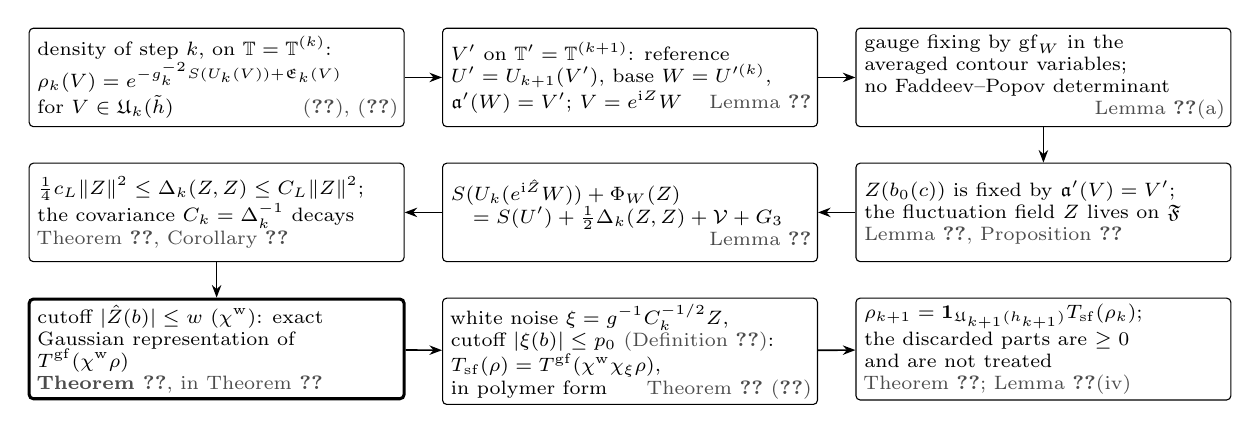
\begin{tikzpicture}[x=1cm,y=1cm,
  st/.style={draw,rounded corners=1.5pt,fill=white,align=flush left,text width=4.55cm,font=\scriptsize,inner xsep=3pt,inner ysep=2pt,minimum height=12.5mm},
  key/.style={st,line width=1.1pt},
  ar/.style={-{Stealth[length=1.6mm]},semithick},
  ]
\def\c#1{\textcolor{black!70}{#1}}
% row 1, left to right
\node[st,anchor=north west] (s1) at (0,0) {density of step $k$, on $\T=\T^{(k)}$:\\ $\rho_k(V)=e^{-g_k^{-2}S(U_k(V))+\mathfrak E_k(V)}$\\ for $V\in\mathfrak U_k(\tilde h)$\hfill\c{\eqref{eq:rho-form}, \eqref{eq:rg-map}}};
\node[st,anchor=north west] (s2) at (5.25,0) {$V'$ on $\T'=\T^{(k+1)}$: reference\\ $U'=U_{k+1}(V')$, base $W=U'^{(k)}$,\\ $\mathfrak a'(W)=V'$; $V=e^{\ii Z}W$\hfill\c{Lemma~\ref{lem:composition}}};
\node[st,anchor=north west] (s3) at (10.5,0) {gauge fixing by $\mathrm{gf}_W$ in the\\ averaged contour variables;\\ no Faddeev--Popov determinant\\ \mbox{}\hfill\c{Lemma~\ref{lem:exp-gauge}(a)}};
% row 2, right to left
\node[st,below=4.5mm of s3] (s4) {$Z(b_0(c))$ is fixed by $\mathfrak a'(V)=V'$;\\ the fluctuation field $Z$ lives on $\mathfrak F$\\ \c{Lemma~\ref{lem:eliminate}, Proposition~\ref{prop:exact-step}}};
\node[st,below=4.5mm of s2] (s5) {$S(U_k(e^{\ii\hat Z}W))+\Phi_W(Z)$\\ \hspace*{1em}$=S(U')+\tfrac12\Delta_k(Z,Z)+\mathcal V+G_3$\\ \mbox{}\hfill\c{Lemma~\ref{lem:step-quadratic}}};
\node[st,below=4.5mm of s1] (s6) {$\tfrac14c_L\|Z\|^2\le\Delta_k(Z,Z)\le C_L\|Z\|^2$;\\ the covariance $C_k=\Delta_k^{-1}$ decays\\ \c{Theorem~\ref{thm:step-coercive}, Corollary~\ref{cor:covariance}}};
% row 3, left to right
\node[key,below=4.5mm of s6] (s7) {cutoff $|\hat Z(b)|\le w$ ($\chi^{\rm w}$): exact\\ Gaussian representation of\\ $T^{\rm gf}(\chi^{\rm w}\rho)$\\ \c{\textbf{Theorem~\ref{thm:step}}, in Theorem~\ref{thm:K}}};
\node[st,below=4.5mm of s5] (s8) {white noise $\xi=g^{-1}C_k^{-1/2}Z$,\\ cutoff $|\xi(b)|\le p_0$ \c{(Definition~\ref{def:small-field-step})}:\\ $T_{\rm sf}(\rho)=T^{\rm gf}(\chi^{\rm w}\chi_\xi\rho)$,\\ in polymer form\hfill\c{Theorem~\ref{thm:sf-step} (\ref{thm:L})}};
\node[st,below=4.5mm of s4] (s9) {$\rho_{k+1}=\one_{\mathfrak U_{k+1}(h_{k+1})}T_{\rm sf}(\rho_k)$;\\ the discarded parts are $\ge0$\\ and are not treated\\ \c{Theorem~\ref{thm:N}; Lemma~\ref{lem:gf-step-invariance}(iv)}};
\foreach \u/\v in {s1/s2,s2/s3,s3/s4,s4/s5,s5/s6,s6/s7,s7/s8,s8/s9} \draw[ar] (\u) -- (\v);
\end{tikzpicture}
\caption{One small-field step, from scale~$k$ to scale~$k+1$, for $k\ge1$ (for $k=0$, Lemma~\ref{lem:first-step-formula} and Proposition~\ref{prop:first-step}); follow the arrows. The gauge fixing and the elimination of the constraint are exact. Theorem~\ref{thm:step} (thick frame) holds for $V'$ of curvature $\eps'_1\le a_{\rm step}$, $w\le r_2$ and $a_1\ge\tilde h\ge2(C_*+1)L^{-2}\eps'_1+4w$. The cutoffs act on the variables of the gauge fixing relative to the base, so the steps define a modified model. Along the flow $w=C_wL^dC_Tg_kp_0(g_k)$ and $4w\le\frac12h_k$ (Remark~\ref{rem:flow-constants}). The blocks and the bonds $b_0(c)$ are drawn in Figures~\ref{fig:blocks-sym} and~\ref{fig:G-scales}.}
\label{fig:G-step}
\end{gfigure}


\paragraph{The step.} Let $\T=\T^{(k)}$ and $\T'=\T^{(k+1)}$, both in the units of step $k$. The map $T$ sends a density $\rho$ of configurations $V$ on $\T$ to the density of the image measure under the one-step averaging $\mathfrak a'$ (\eqref{eq:rg-map}). Fix $V'$ on $\T'$ with small curvature, and let $U'=U_{k+1}(V')$ be its background field, the \emph{reference} of the step. The \emph{base} is $W=U'^{(k)}$, the $k$-fold average of the reference, a configuration on $\T$ with $\mathfrak a'(W)=V'$. The configurations of the step are written $V=e^{\ii Z}W$.

\paragraph{Gauge fixing and coordinates.} Following Ba\l aban, $\mathrm{gf}_W$ is a product over the blocks of Gaussian weights $e^{-|u-1|^2/2g^2}$ in the averaged contour variables relative to $W$ (Definition~\ref{def:gauge-fixing}). By a Faddeev--Popov identity without determinant, inserting it changes no integral of an invariant integrand supported on regular configurations (Lemma~\ref{lem:exp-gauge}(a)). The constraint $\mathfrak a'(e^{\ii Z}W)=V'$ is solved for $Z$ on the middle bond $b_0(c)$ of each coarse bond $c$, with local Jacobians $\mathfrak j_c$ (Lemma~\ref{lem:eliminate}); the free variables live on the set $\mathfrak F$ of the other bonds (Definition~\ref{def:bonds}). With these coordinates the gauge-fixed step is, for $\rho$ of the form \eqref{eq:rho-form} with threshold $\tilde h$ and $g=g_k$ (Theorem~\ref{thm:step}),
\[
\begin{aligned}
T^{\rm gf}(\chi^{\rm w}\rho)(V')={}&\mathcal N_k\exp\Big(-\frac1{g^2}S(U')-\frac12\sum_{b\in\mathfrak F}\ell_k(b)+\sum_c\log\mathfrak j_c\Big)\\
&\times\int d\mu_{C_k}(Y)\,\chi^{\rm w}\big(\hat Z(gY)\big)\exp\Big(-\frac{(\mathcal V+G_3)(gY)}{g^2}+\mathfrak J(gY)+\mathfrak E\big(e^{\ii\hat Z(gY)}W\big)\Big).
\end{aligned}
\]
Here $\mu_{C_k}$ is the Gaussian measure on the fields on $\mathfrak F$ with covariance $C_k=\Delta_k^{-1}$; $\mathcal V+G_3$ is an interaction of third order; and $\mathfrak E$ is the old part of the density.

\paragraph{Coercivity.} The covariance exists and decays because $\frac14c_L\|Z\|^2\le\Delta_k(Z,Z)\le C_L\|Z\|^2$ (Theorem~\ref{thm:K}(ii)). The constant $c_L$ depends only on $d$ and $L$. It comes from a Poincar\'e inequality for one step (Lemma~\ref{lem:poincare-step}). The gauge-fixing term is necessary in it.

\paragraph{A curvature bound independent of $L$.} The curvature of a background field is at most $(C_*+\delta)$ times the curvature of the coarse configuration, where $C_*$ depends only on $a$, $\alpha$ and $G$ (Proposition~\ref{prop:sharp-curvature}). This makes the small-field sets of consecutive steps compatible as soon as $L^2\ge8(C_*+1)$, given $h_{k+1}\le2h_k$ (Lemma~\ref{lem:composition}(a), Remark~\ref{rem:parameters}(2)).

\paragraph{The cutoffs and the modified model.} The small-field step is $T_{\rm sf}(\rho)=T^{\rm gf}(\chi^{\rm w}\chi_\xi\rho)$, with two bondwise cutoffs: $\chi^{\rm w}$ bounds the field $Z$ relative to the base by $w$ (Definition~\ref{def:chi-w}), and $\chi_\xi$ bounds the white noise $\xi=g^{-1}C_k^{-1/2}Z$ by $p_0$ (Definition~\ref{def:small-field-step}). The cutoffs $\chi^{\rm w}$ and $\chi_\xi$ are not invariant under the gauge transformations of the blocks, so the small-field steps define a modified model (Remark~\ref{rem:sf-reference}(c)). What a step discards is nonnegative (Theorem~\ref{thm:K}(iii)), so the partition function of the small-field model is at most that of the lattice theory with the same counterterm (Remark~\ref{rem:sf-reference}(c)). The large-field stage, which starts from the discarded parts, is not treated (Remark~\ref{rem:sf-reference}(d)).

\paragraph{Where in the note.} Sections~\ref{sec:rg-step}--\ref{sec:covariance}. In the companion: the chapter on Part~VII.

\gsection{Localization (Parts~VIII--IX)}\label{g:localization}

The step of Part~VII depends on the background on the whole torus: through the covariance $C_k$, the coarse Hessian, the determinant $\det\Delta_k$, and the background field of the configuration that is integrated. A polymer expansion needs each of these as a sum of local pieces, analytic and gauge invariant, with a small factor for every cube of the region on which a piece depends. Parts~VIII and~IX provide this.
\begin{itemize}
\item \emph{Radius type.} A piece that depends on the background in a ball of radius $m$ is bounded by $e^{-\gamma m}$. Dirichlet approximants on growing domains, followed by telescoping, give this form (Theorem~\ref{thm:local-covariance}).
\item \emph{Volume type.} A piece that depends on a polymer $X$ carries a small factor for every box of $X$. It comes from random walks with weakening parameters (Definition~\ref{def:weak-family}, Theorem~\ref{thm:weak-inverse}), and the localization lemma turns it into pieces with a factor $e^{-(\kappa-1)}$ per box (Lemma~\ref{lem:localization}).
\end{itemize}

\paragraph{What Part~VIII keeps.} Part~VIII is written for radius-type locality, which Parts~IX and~X supersede. On the main line stay the Dirichlet averaged operators (Proposition~\ref{prop:dirichlet-averaged}), their interior bounds (Theorem~\ref{thm:ID}), the Dirichlet Hessians (Propositions~\ref{prop:dirichlet-hessian} and~\ref{prop:local-fluct}) and the graded domains of the activities (Definition~\ref{def:graded}, Lemma~\ref{lem:quadratic-bound}); the reading guide in Section~\ref{sec:intro} lists the results off the main line.

\paragraph{Weakened walks (Sections~\ref{sec:weakenable}--\ref{sec:nested-walks}).} Each box $\Box$ of a paving carries a weakening parameter $s_\Box$ in a disc $\mathbb D_\kappa$. A \emph{weakenable family} is a sum $O(s)=\sum_\omega s^{n_\omega}O_\omega$ over polymers $X_\omega$, where $O_\omega$ depends on the data only near $X_\omega$ and the monomial $s^{n_\omega}$ involves exactly the boxes of $X_\omega$ (Definition~\ref{def:weak-family}). The inverse on a domain $X$ is a Neumann series around a parametrix made of local Dirichlet inverses on the domains $\Lam^v_j$, the unions of the blocks within distance $\rho M$ of the grid points $z_j$ (Section~\ref{sec:weakenable}), and each step of the walk carries the monomial $s^{X(j)}$ of a union $X(j)$ of boxes. Under the hypotheses (W1)--(W3) and that of Lemma~\ref{lem:step-small}, and for $M$ large, this series is a weakenable family that represents the inverse (Theorem~\ref{thm:weak-inverse}). The walks are nested at five levels, (L1)--(L5), from the scalar Green function to the resolvents of the fluctuation operator, because the non-local part of each operator is built from inverses of earlier levels (Section~\ref{sec:nested-walks}). Each walk costs at most $2\delta$ in the rate $\kappa$, and each product at most $\delta$ (Corollary~\ref{cor:weak-covariance}).

\paragraph{Outputs.} The weakened square root $C_k^{1/2}(s)$ of the covariance and the determinant densities $\ell_k(b)$ are weakenable families (Corollary~\ref{cor:weak-covariance}). The one-loop source is a sum over polymers, $-\frac12\log\det\Delta_k(U)=-\frac12\log\det\Delta_k(1)+\sum_X\mathfrak e(X,U)$, of normalized graded activities with volume decay, quadratically small in the curvature (Proposition~\ref{prop:one-loop-polymer}). On the domain of the next step this quadratic part is marginal in four dimensions, so it must be extracted as a coupling constant, not bounded (Remark~\ref{rem:one-loop-polymer}(b)).

\paragraph{Tiers and the background map (Sections~\ref{sec:pointwise-weak}--\ref{sec:weak-background}).} The weakened background map needs pointwise $C^{1,\alpha}$ bounds for the weakened $\bH(s)$, $\bC(s)$ and $\bC(s)D^T$, uniformly on $\mathbb D_\kappa$ (\eqref{eq:pointwise-needed}). In four dimensions $L^2$ data sit at the endpoint $p=\frac d2$, so the last interior factors of a walk term raise them along $L^2\to L^4\to L^8\to C^{1,\beta}$ (Lemmas~\ref{lem:int-factors} and~\ref{lem:endpoint-factors}). The results are Theorems~\ref{thm:tier-walk} and~\ref{thm:HC-pointwise}, at level (L3) with $W=0$ and with $\beta=\min(\alpha,\frac12)$. With these bounds, the background map becomes the fixed point $A_*(s;B)$ of a weakened contraction (Theorem~\ref{thm:weak-bg}). It is analytic in $(s,B)$. At $s=1$ and a critical reference it is the background map of Part~V. If $s_\Box=0$ outside a union of boxes, it factorizes over the components of that union.

\paragraph{Where in the note.} Part~VIII: Sections~\ref{sec:dirichlet-averaged}--\ref{sec:interaction-local}. Part~IX: Sections~\ref{sec:weakenable}--\ref{sec:weak-background}. In the companion: the chapters on Part~VIII and on Part~IX.

\gsection{The step in polymer form (\texorpdfstring{Sections~\ref{sec:complex-references}--\ref{sec:cluster}}{Sections 46-48})}\label{g:polymer}

Sections~\ref{sec:complex-references}--\ref{sec:cluster} turn the exact Gaussian form of one step (Theorem~\ref{thm:step}) into polymer form. The result is Theorem~\ref{thm:sf-step}, which is Theorem~\ref{thm:L}(i). At real critical references, with $V'$ small field,
\[
\begin{aligned}
T_{\rm sf}(\rho)(V')=\mathcal N_kN_\chi\exp\Big(&-\frac1{g^2}S(U')-\frac12\sum_b\ell_k(b;1)+\sum_X\mathfrak e(X,U')+\sum_c\log\mathfrak j_c\\
&+\mathfrak E(U')+\sum_Y\big(E^\#_{\rm p}(Y,U')+E^\#_{\rm m}(Y,U')\big)\Big).
\end{aligned}
\]
Every term depends on $U'$ only near its polymer, is invariant under real gauge transformations, is real at real references, and is analytic in the reference on complex domains. On the domains of Remark~\ref{rem:domain-constants} the one-loop activities are bounded by $Ce^{-(\kappa_2-1)|X|}$ and the Jacobian terms by $C$, with $C$ independent of the coupling; their quadratic parts are marginal. The pure sources $E^\#_{\rm p}$ are of order $g^2p_0^6$, and the mixed sources $E^\#_{\rm m}$ are bounded by the old activities. The hypotheses of Theorem~\ref{thm:sf-step} on the coupling, the thresholds and the old activities are supplied along the flow by Theorem~\ref{thm:N}(v) (Table~\ref{tab:G-supply}).

\paragraph{Complex references (Section~\ref{sec:complex-references}).} The activities of the flow must be analytic in the background on the graded domains (Definition~\ref{def:graded}). So the step evaluates the operators of Part~IX, the interior estimates and the weakened background map at complex references $U=e^{\ii\eta A'}U_r$, with $U_r$ real and regular and $A'$ small. Three mechanisms carry them over (Proposition~\ref{prop:complex-ext}).
\begin{itemize}
\item \emph{Identities from the real points.} An exact identity proved at real backgrounds extends to a convex ball of complex references by the identity theorem, since the real points of the ball are real backgrounds (Remark~\ref{rem:general-averaging}, last paragraph).
\item \emph{Fixed coercivity constants and rates.} The coercivity constants and the decay rates do not depend on the size $\delta_c$ of the complex part.
\item \emph{Monotone majorants.} At complex references of size $\delta_c<\delta_P$ the other constants are at most twice their real values.
\end{itemize}
The thresholds are fixed in an order that avoids circularity: the cap $\bar\delta$ and the threshold $\eps_{\max}$ first, then $\delta_P$ (Remark~\ref{rem:parameters}(4),(5)). In four dimensions the constants $\theta_r$, $\delta_1$, $\delta_0$ of the graded domains do not depend on the coupling, the step, the torus or the polymer (Remark~\ref{rem:domain-constants}).

\paragraph{Step quantities and the fluctuation integral (Sections~\ref{sec:step-quantities}--\ref{sec:cluster}).} The ingredients of the step become functions of the weakening parameters that factorize over polymers (Propositions~\ref{prop:interaction-pieces}, \ref{prop:gf-pieces}, \ref{prop:jacobians}, \ref{prop:composed} and~\ref{prop:hessian-general}). The localization lemma then writes each of them, at $s=1$, as a sum of pieces with a factor $e^{-(\kappa-1)}$ for every box beyond the polymer (Lemma~\ref{lem:localization}). The fluctuation integral follows Dimock's small-field scheme \cite{DimockI}.
\begin{itemize}
\item \emph{White noise.} The fluctuation is written $Z=gC_k^{1/2}\xi$, and the small-field condition is imposed on $\xi$: $|\xi(b)|\le p_0$ on every bond of $\mathfrak F$ (Definition~\ref{def:small-field-step}). On this set the fluctuation cutoff $\chi^{\rm w}$ equals $1$, every step quantity is defined, and the composed configurations stay in the domains of the old activities (Lemma~\ref{lem:white-noise}).
\item \emph{Mayer and polymer expansion.} The localized pieces (Proposition~\ref{prop:localized-pieces}) are integrated by a Mayer expansion with the Kotecký--Preiss criterion (Theorem~\ref{thm:mayer}). The output splits into a pure class, from the interaction, gauge-fixing and Jacobian pieces alone, and a mixed class, which involves the old activities (Corollary~\ref{cor:two-classes}).
\item \emph{Parity.} Replace $g$ by a complex parameter $t$ in the fluctuation. The pure pieces are even under $(t,\xi)\mapsto(-t,-\xi)$ and vanish at $t=0$, so the pure output divided by $t^2$ is analytic. Cauchy's estimate gives $E^\#_{\rm p}=O(g^2p_0^6)$, with no term of order $g$ (Proposition~\ref{prop:pure-sources}).
\end{itemize}
Section~\ref{sec:cluster} assumes three conditions (Q1)--(Q3) on the small-field parameters. Along the flow, (Q1) and (Q3) hold by condition ($\Gamma$2) on the bound $\gamma$ of the couplings, and (Q2) holds for the next threshold as long as $g_{k+1}\le\min(2g_k,\gamma)$ (the paragraph after (Q1)--(Q3) in Section~\ref{sec:cluster}; Remark~\ref{rem:flow-constants}).

\paragraph{Where in the note.} Sections~\ref{sec:complex-references}--\ref{sec:cluster}; the first step and the vacuum energy are in Section~\ref{sec:target-flow} (Theorem~\ref{thm:L}(ii),(iii)). In the companion: the chapter on the first half of Part~X.

\gsection{The four-dimensional flow (\texorpdfstring{Sections~\ref{sec:flow}--\ref{sec:flow4}}{Sections 49-53})}\label{g:flow}

Sections~\ref{sec:flow}--\ref{sec:flow4} iterate the step of Theorem~\ref{thm:sf-step} over all scales at which the couplings stay in $(0,\gamma]$, in Ba\l aban's generation form, on a fixed torus. The result is Theorem~\ref{thm:sf-flow}, summarized as Theorem~\ref{thm:N}. It is a theorem about the small-field model of Remark~\ref{rem:sf-reference}(c) on the given torus; the large-field stage is not treated (Remark~\ref{rem:sf-flow}(d)).

\paragraph{Why generations.} The new activities of a step are of order one, not small in the coupling, and their quadratic part in the curvature is marginal in four dimensions (Remark~\ref{rem:one-loop-polymer}(b)). So the effective action of a step is not turned into a single activity of the next scale and contracted. Following Ba\l aban, the new terms of each step are kept as a separate \emph{generation}, bounded only at its creation scale (Remark~\ref{rem:flow-status}, the opening of Section~\ref{sec:generations}). At every later scale its marginal part is cancelled by a counterterm $-\beta_jS$, with $g_{j+1}^{-2}=g_j^{-2}-\beta_{j+1}$, and what remains is small by explicit gains. The iteration needs no contraction. The smallness of what a step adds beyond the one-loop and Jacobian terms comes from the fluctuation cutoff and from parity (Remark~\ref{rem:flow-status}, Proposition~\ref{prop:pure-sources}). Figure~\ref{fig:G-generation} shows the life of a generation.

% Figure of the guide (G9): the life of a generation in the flow (Sections 50--53). Owner: WP7.
\begin{gfigure}[tp]
\centering
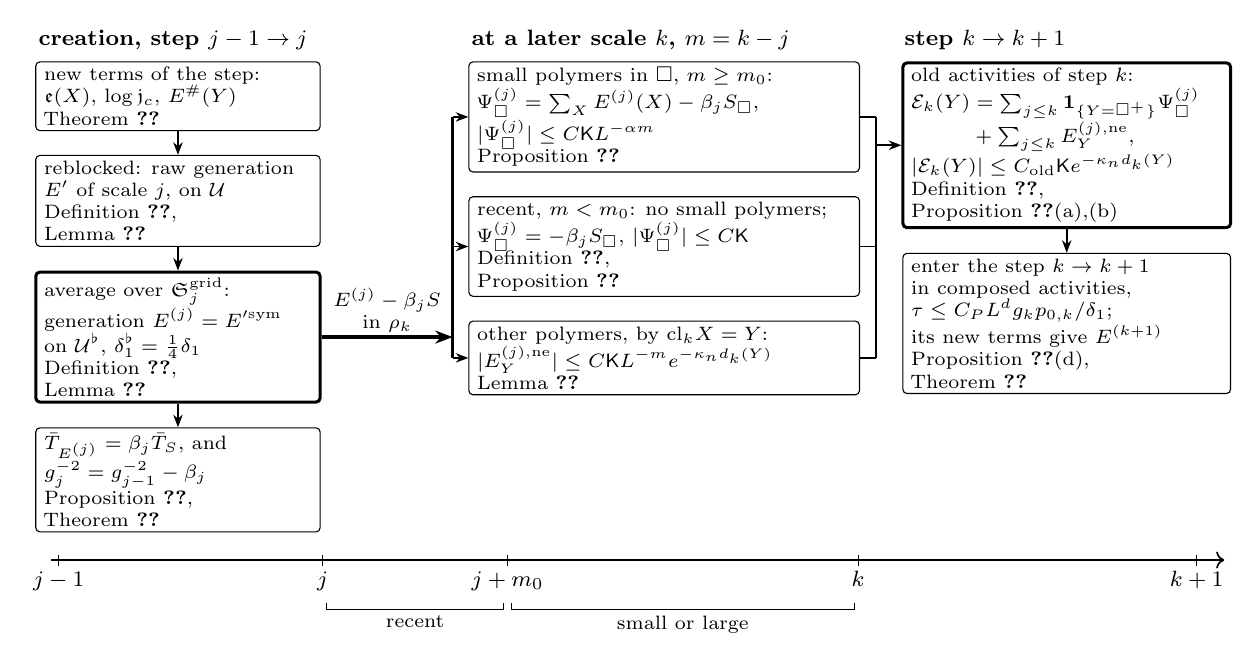
\begin{tikzpicture}[x=1cm,y=1cm,
  bx/.style={draw,rounded corners=1.5pt,fill=white,align=flush left,font=\scriptsize,inner xsep=3pt,inner ysep=2pt},
  hd/.style={font=\footnotesize\bfseries,anchor=south west,inner sep=1pt},
  ar/.style={-{Stealth[length=1.6mm]},semithick},
  big/.style={-{Stealth[length=2.2mm]},line width=1.2pt},
  ]
% creation of the generation, in the step from j-1 to j
\node[hd] at (0.1,0.1) {creation, step $j-1\to j$};
\node[bx,text width=3.4cm,anchor=north west] (c1) at (0.1,0) {new terms of the step:\\ $\mathfrak e(X)$, $\log\mathfrak j_c$, $E^\#(Y)$\\ Theorem~\ref{thm:sf-step}};
\node[bx,text width=3.4cm,below=3mm of c1] (c2) {reblocked: raw generation\\ $E'$ of scale $j$, on $\mathcal U$\\ Definition~\ref{def:raw-new},\\ Lemma~\ref{lem:raw-new}};
\node[bx,text width=3.4cm,below=3mm of c2,line width=1.1pt] (c3) {average over $\mathfrak S^{\rm grid}_j$:\\ generation $E^{(j)}=E'^{\rm sym}$\\ on $\mathcal U^\flat$, $\delta_1^\flat=\frac14\delta_1$\\ Definition~\ref{def:symmetrization},\\ Lemma~\ref{lem:symmetrization}};
\node[bx,text width=3.4cm,below=3mm of c3] (c4) {$\bar T_{E^{(j)}}=\beta_j\bar T_S$, and\\ $g_j^{-2}=g_{j-1}^{-2}-\beta_j$\\ Proposition~\ref{prop:period-iso},\\ Theorem~\ref{thm:gen-step}};
\foreach \u/\v in {c1/c2,c2/c3,c3/c4} \draw[ar] (\u) -- (\v);
% a later scale k
\node[hd] at (5.6,0.1) {at a later scale $k$, $m=k-j$};
\node[bx,text width=4.75cm,anchor=north west] (l1) at (5.6,0) {small polymers in $\Box$, $m\ge m_0$:\\ $\Psi^{(j)}_\Box=\sum_XE^{(j)}(X)-\beta_jS_\Box$,\\ $|\Psi^{(j)}_\Box|\le C\mathsf KL^{-\alpha m}$\\ Proposition~\ref{prop:extraction}};
\node[bx,text width=4.75cm,below=3mm of l1] (l2) {recent, $m<m_0$: no small polymers;\\ $\Psi^{(j)}_\Box=-\beta_jS_\Box$, $|\Psi^{(j)}_\Box|\le C\mathsf K$\\ Definition~\ref{def:polymer-classes},\\ Proposition~\ref{prop:extraction}};
\node[bx,text width=4.75cm,below=3mm of l2] (l3) {other polymers, by $\mathrm{cl}_kX=Y$:\\ $|E^{(j),\rm ne}_Y|\le C\mathsf KL^{-m}e^{-\kappa_nd_k(Y)}$\\ Lemma~\ref{lem:large-later}};
% the old activities, and the next step
\node[hd] at (11.1,0.1) {step $k\to k+1$};
\node[bx,text width=3.95cm,anchor=north west,line width=1.1pt] (o) at (11.1,0) {old activities of step $k$:\\ $\mathcal E_k(Y)=\sum_{j\le k}\one_{\{Y=\Box^+\}}\Psi^{(j)}_\Box$\\ \hphantom{$\mathcal E_k(Y)$}${}+\sum_{j\le k}E^{(j),\rm ne}_Y$,\\ $|\mathcal E_k(Y)|\le C_{\rm old}\mathsf Ke^{-\kappa_nd_k(Y)}$\\ Definition~\ref{def:old-activities},\\ Proposition~\ref{prop:old-activities}(a),(b)};
\node[bx,text width=3.95cm,below=3mm of o] (s) {enter the step $k\to k+1$\\ in composed activities,\\ $\tau\le C_PL^dg_kp_{0,k}/\delta_1$;\\ its new terms give $E^{(k+1)}$\\ Proposition~\ref{prop:old-activities}(d),\\ Theorem~\ref{thm:gen-step}};
% arrows
\draw[semithick] ([xshift=2mm]l1.east) -- ([xshift=2mm]l1.east |- l3.east);
\foreach \u in {l1,l2,l3} \draw[semithick] (\u.east) -- ([xshift=2mm]l1.east |- \u.east);
\draw[ar] ([xshift=2mm]l1.east |- o.west) -- (o.west);
\draw[ar] (o) -- (s);
\draw[line width=1.2pt] ([xshift=-2mm]l1.west) -- ([xshift=-2mm]l1.west |- l3.west);
\draw[big] (c3.east) -- node[above,font=\scriptsize,align=flush center,inner sep=1pt] {$E^{(j)}-\beta_jS$\\ in $\rho_k$} ([xshift=-2mm]l1.west |- c3.east);
\foreach \u in {l1,l2,l3} \draw[ar] ([xshift=-2mm]l1.west |- \u.west) -- (\u.west);
% scale axis
\path let \p1=(c4.south), \p2=(l3.south), \p3=(s.south) in coordinate (ax) at (0,{min(\y1,\y2,\y3)-0.35cm});
\draw[->,semithick] ([xshift=3mm]ax) -- (ax -| 15.2,0);
\foreach \x/\l in {0.4/{j-1},3.75/j,6.1/{j+m_0},10.55/k,14.85/{k+1}} {
  \draw ([xshift=\x cm]ax) ++(0,0.07) -- ++(0,-0.14) node[below,font=\footnotesize,inner sep=2pt] {$\l$};}
\draw ([shift={(3.8,-0.55)}]ax) -- ++(0,-0.08) -- node[below,font=\scriptsize,inner sep=2pt] {recent} ++(2.25,0) -- ++(0,0.08);
\draw ([shift={(6.15,-0.55)}]ax) -- ++(0,-0.08) -- node[below,font=\scriptsize,inner sep=2pt] {small or large} ++(4.35,0) -- ++(0,0.08);
\end{tikzpicture}
\caption{The life of a generation in the flow; the axis is the scale. Left, the step from scale $j-1$ to scale $j$: its new terms, reblocked, form the raw generation $E'$; its average over the symmetries of the grid of scale $j$ is the generation $E^{(j)}$, bounded at its creation scale by $\mathsf Ke^{-\kappa_nd_j(X)}$ on the domains $\mathcal U^\flat(X)$ (Theorem~\ref{thm:N}(ii)); its period density gives the coefficient $\beta_j$ and the coupling $g_j$. The density $\rho_k$ of every later scale contains $E^{(j)}-\beta_jS$ (Theorem~\ref{thm:N}(i)). Middle, a later scale $k$ and a grid cube $\Box$ of scale $k$: a polymer of scale $j$ is recent, small or large at scale $k$ (Definition~\ref{def:polymer-classes}). The counterterm $-\beta_jS_\Box$ is grouped with the small polymers of $E^{(j)}$ in $\Box$, and the sum is bounded on $\mathcal U^\flat(\Box^+)$, by $C\mathsf KL^{-\alpha m}$ for $m\ge m_0$; the other polymers gain $L^{-m}$ (Theorem~\ref{thm:N}(iv)). Right, the old activities collect the generations $j\le k$ and enter the step from scale $k$ to scale $k+1$, whose new terms form the next generation. The bounds hold for couplings in $(0,\gamma]$; $C$, $C_{\rm old}$ and $\mathsf K$ do not depend on $j$, $k$, the torus or the couplings (Theorem~\ref{thm:N}, Proposition~\ref{prop:old-activities}).}
\label{fig:G-generation}
\end{gfigure}


\paragraph{Polymer grids (Section~\ref{sec:flow}).} Activities are functions on the fine lattice, the same lattice at every scale (Section~\ref{subsec:flow-norm}). The polymer grid of scale $j$ consists of Ba\l aban's cubes of side $M$; polymers are unions of grid cubes, and $d_j(X)$ is their tree length. The grids of different scales are aligned (Lemma~\ref{lem:grid-nesting}), and reblocking keeps the decay rate (Lemma~\ref{lem:reblocking}, Remark~\ref{rem:parameters}). Seen from a later scale $k=j+m$, a polymer of scale $j$ is \emph{recent} if $m<m_0$, \emph{small} if $m\ge m_0$ and $d_j(X)\le c'm$, and \emph{large} otherwise (Definition~\ref{def:polymer-classes}).

\paragraph{A generation (Section~\ref{sec:generations}).} A generation of scale $j$ is a family $E=\{E(X,\cdot)\}$ of normalized, gauge-invariant graded activities on the polymers of scale $j$, on the domains $\mathcal U^\flat(X)$, real at real configurations (G1), covariant under the translations (G2) and all symmetries $\mathfrak S^{\rm grid}_j$ (G4) of the grid, whose sum at the background fields of scale $j$ is invariant under $\mathfrak S_j$ (G3) (Definition~\ref{def:generation}). Its norm is $\|E\|_j=\sup_Xe^{\kappa_nd_j(X)}\sup_{\mathcal U^\flat(X)}|E(X,\cdot)|$. At a later scale $k$ the generation is evaluated at $U_k(V)$, which is a background field of scale $j$ of a configuration in the small-field set of scale $j$ (Lemma~\ref{lem:later-small-field}). So the sum and its symmetry persist.

\paragraph{Symmetrization and the coefficient $\beta$.} The new terms of a step, reblocked, form a raw generation: it has (G1), on the larger domains $\mathcal U(X)$, and (G3), but the step does not make it covariant under the grid symmetries (Definition~\ref{def:raw-new}, Lemma~\ref{lem:raw-new}, the opening of Section~\ref{sec:generations}). Its average over $\mathfrak S^{\rm grid}_j$ is a generation with the same sum at the background fields and no larger norm (Definition~\ref{def:symmetrization}, Lemma~\ref{lem:symmetrization}). The price is a smaller domain, $\delta_1^\flat=\frac14\delta_1$: a reflection turns forward differences into backward ones, which at a curved real part costs a factor and a plaquette term (Lemma~\ref{lem:grid-domains}, Remark~\ref{rem:symmetrization-flow}(d)). The coefficient of a generation is read off from its \emph{period density} $\bar T_E$, the second variation of its activities at the linear fields of constant curvature $F$, per unit volume (Definition~\ref{def:period-density}). By (G4) and the gauge invariance of the activities it is a quadratic form invariant under $B_4$ and under conjugation by $G$. For simple $G$ such a form is a multiple of the action's (Lemma~\ref{lem:b4-forms}): $\bar T_E=\beta_E\bar T_S$, with $\beta_E$ real and $|\beta_E|\le C_\beta\|E\|_j$, and there is no topological and no anisotropic part (Proposition~\ref{prop:period-iso}). The flow uses the simplicity of $G$ here.

\paragraph{Extraction at later scales (Section~\ref{sec:extraction}).} Let $m=k-j\ge m_0$. On a small polymer $X$ of scale $j$, a configuration of the domain of scale $k$ is, in a complex gauge built in three stages (real, then affine, then quadratic), a linear field of constant curvature $F_X$ plus a remainder of order $L^{-(2+\alpha)m}$ (Lemma~\ref{lem:later-normal-form}(a),(b)). So $E(X,U)$ is a quadratic form in $F_X$ up to $O(L^{-(4+\alpha)m})$ (Lemma~\ref{lem:later-normal-form}(d)). Summed over the small polymers based in a grid cube $\Box$ of scale $k$, which contains $L^{4m}$ grid cubes of scale $j$, these quadratic forms add up to $M^4\sum_Q\bar T_E(F_Q)$ over the cubes $Q$ of scale $j$ in $\Box$ (Lemma~\ref{lem:cell-sums}), and the counterterm $\beta_ES_\Box$ cancels them. The error is $C_{\rm ex}\|E\|_jL^{-\alpha m}$ (Proposition~\ref{prop:extraction}). The polymers that are not small carry a gain $L^{-m}$ (Lemma~\ref{lem:large-later}), and the wrapping ones are bounded at all later scales (Lemma~\ref{lem:torus}(c)--(e)).

\paragraph{Old activities and one step (Section~\ref{sec:flow4}).} In every grid cube $\Box$ of scale $k$ the counterterm $-\beta_jS_\Box$ is grouped with the small polymers of generation $j$ based in $\Box$; the other polymers are grouped by their closure at scale $k$ (Definition~\ref{def:old-activities}). For a recent generation the whole counterterm enters the old activity. The resulting \emph{old activities} $\mathcal E_k$ are bounded by $C_{\rm old}\mathsf K$ with decay, uniformly in $k$, $K$, the torus and the couplings. Their sum at a background field is $\sum_{j\le k}(E^{(j)}-\beta_jS)$, and they satisfy the hypothesis of Theorem~\ref{thm:sf-step} on old activities (Proposition~\ref{prop:old-activities}). One step then preserves the generation form, with $g_{k+1}^{-2}=g_k^{-2}-\beta_{k+1}$ and $g_{k+1}\le2g_k$ (Theorem~\ref{thm:gen-step}; the first step is Proposition~\ref{prop:gen-one}). The generations and the coefficients depend only on the earlier couplings $(g_0,\dots,g_{j-1})$, and continuously (Proposition~\ref{prop:flow-continuity}, Corollary~\ref{cor:bare-continuity}).

\paragraph{Theorem~\ref{thm:sf-flow} in words.} Let $G$ be compact, connected and simple. Choose the parameters in the order of Remark~\ref{rem:parameters}, a bound $\gamma$ on the couplings with ($\Gamma$1)--($\Gamma$3) of Remark~\ref{rem:flow-constants}, and a torus whose side at the last scale is $n_K\ge n_{\min}$, with $\ell L^N$ a power of $L$ (Section~\ref{subsec:tf-scales}). Start from $\rho_0=\exp(-g_0^{-2}S-E_0)$ with $g_0\in(0,\gamma]$. Let the generations, the coefficients and the couplings be defined by the recursion of the steps, and put $\rho_j=\one_{\mathfrak U_j(h_j)}T_{\rm sf}(\rho_{j-1})$ as long as $g_1,\dots,g_j\le\gamma$. Then, at every scale $k\le K$ that the recursion reaches in this way, whatever the later couplings:
\begin{itemize}
\item[(a)] the density has the generation form $\mathcal Z_k\exp(-g_k^{-2}S(U_k)-\eps_k|\T^{(k)}|+\sum_{j\le k}(E^{(j)}-\beta_jS)(U_k))$ on the small-field set, and vanishes outside it;
\item[(b)] every generation is bounded at its creation scale by $\mathsf Ke^{-\kappa_nd_j(X)}$, on domains whose constants do not depend on the coupling;
\item[(c)] its period density is exactly isotropic, and $|\beta_j|\le C_\beta\mathsf K$;
\item[(d)] at every later scale its small polymers in a grid cube differ from $\beta_jS_\Box$ by at most $C_{\rm ex}\mathsf KL^{-\alpha m}$ ($C_{\rm ex}\mathsf K$ for recent generations), and the whole sum $\sum_j(E^{(j)}-\beta_jS)$ at a background field is at most a constant times $\mathsf K$ per site;
\item[(e)] consecutive couplings satisfy $|g_j^{-2}-g_{j-1}^{-2}|\le C_\beta\mathsf K$ and $\frac34g_{j-1}\le g_j\le2g_{j-1}$, and every step satisfies the hypotheses of Theorem~\ref{thm:sf-step} (of Proposition~\ref{prop:first-step} for the first step);
\item[(f)] if all couplings up to scale $K$ stay below $\gamma$, there is exactly one $E_0$ with $\eps_K=0$, and then $|\eps_k|\le C'_{\rm vac}g_kp_{0,k}$.
\end{itemize}
The constants depend only on the parameters fixed before $\gamma$ ($C'_{\rm vac}$ also on the function $p_0$), not on $k$, $K$, the torus or the couplings. The stability bound adds that, for the counterterm with $\eps_K=0$, the partition function of the small-field model is, up to the explicit normalization $\mathcal Z_K$, between $e^{-c|\T^{(K)}|}$ and $e^{c|\T^{(K)}|}$; the constant $c$ depends on $g_K$ and on the parameters, not on $K$, the torus or the earlier couplings (Corollary~\ref{cor:sf-stability}). Bounds per volume suffice because the final torus is fixed (Remark~\ref{rem:sf-reference}(a)).

\paragraph{Concordance.} Theorem~\ref{thm:N}(i)--(v) are Theorem~\ref{thm:sf-flow}(a)--(e), with Proposition~\ref{prop:period-iso} in~(iii) and Proposition~\ref{prop:extraction} and Lemma~\ref{lem:large-later} in~(iv); (vi) is (f) with Corollary~\ref{cor:sf-stability}; (vii) is Proposition~\ref{prop:flow-continuity} with Corollary~\ref{cor:bare-continuity}. Items (a), (b) and (d) correspond to Ba\l aban's (0.22)--(0.24), (0.25) and (0.28)--(0.30) \cite{BalYM4I}, and Theorem~\ref{thm:N} is the analogue, for the small-field model on the torus, of his Theorem~3 (the paragraph after Theorem~\ref{thm:N}).

\paragraph{What the theorem does not say.} No asymptotic behaviour of the couplings is assumed. The theorem bounds $|\beta_j|$ but does not control its sign; Part~XI controls the sums of the $\beta_j$ through the one-loop coefficient (Section~\ref{g:oneloop}). The dependence on the couplings is a dependence on the whole sequence $(g_0,\dots,g_{j-1})$, and only its continuity is proved. The small-field domain shrinks with the coupling, as in Dimock's scheme (Remark~\ref{rem:sf-flow}(a)).

\paragraph{Who supplies the hypotheses.} The main theorems take their hypotheses from later Parts. Table~\ref{tab:G-supply} lists, for Theorems~\ref{thm:K}, \ref{thm:L} and~\ref{thm:N}, each hypothesis and the result that supplies it along the flow. All conditions on $\gamma$ are upper bounds by quantities fixed before $\gamma$, so they hold together for $\gamma$ small (Remark~\ref{rem:parameters}(6), Remark~\ref{rem:flow-constants}, Feasibility).

\begin{table}[htbp]
\centering\small
\renewcommand{\arraystretch}{1.2}
\begin{tabular}{@{}p{0.12\textwidth}p{0.4\textwidth}p{0.4\textwidth}@{}}
\hline
\raggedright Theorem & \raggedright Hypothesis & \raggedright Supplied by \tabularnewline
\hline
\raggedright \ref{thm:K} (one step) & \raggedright $G$ compact, connected, semisimple & \raggedright Theorem~\ref{thm:N} assumes $G$ simple \tabularnewline
 & \raggedright $M\ge\max(M_0,5L)$ & \raggedright Remark~\ref{rem:parameters}(4) \tabularnewline
 & \raggedright side of the torus & \raggedright (T0)--(T2), from $n_K\ge n_{\min}$ and $\ell L^N$ a power of $L$ (Section~\ref{subsec:tf-scales}, Lemma~\ref{lem:torus}(a)) \tabularnewline
 & \raggedright curvature of $V'$ at most $\eps'_1\le a_{\rm step}$ & \raggedright $\eps'_1=h_{k+1}\le\gamma p(\gamma)\le a_{\rm step}$, by ($\Gamma$2) \tabularnewline
 & \raggedright $w\le r_2$ & \raggedright (Q1), by ($\Gamma$2) \tabularnewline
 & \raggedright density of the form \eqref{eq:rho-form}, with $a_1\ge\tilde h\ge2(C_*+1)L^{-2}\eps'_1+4w$ & \raggedright Theorem~\ref{thm:gen-step}(a) with $\tilde h=h_k$; the inequality is (Q2), from $g_{k+1}\le\min(2g_k,\gamma)$ (Theorem~\ref{thm:gen-step}(c),(d)) \tabularnewline
\hline
\raggedright \ref{thm:L} (step in polymer form) & \raggedright $\alpha\le\frac12$; parameters as in Remark~\ref{rem:parameters} & \raggedright Remark~\ref{rem:parameters}(4); assumption of Theorem~\ref{thm:N} \tabularnewline
 & \raggedright (Q1), (Q3), $2g\le r_t$ & \raggedright ($\Gamma$2) of Remark~\ref{rem:flow-constants} \tabularnewline
 & \raggedright (Q2) with $\eps'_1=h_{k+1}$ & \raggedright Theorem~\ref{thm:gen-step}(d) \tabularnewline
 & \raggedright (DC5) & \raggedright the domain constants, Remark~\ref{rem:parameters}(5) \tabularnewline
 & \raggedright decay and bound of the old activities & \raggedright Proposition~\ref{prop:old-activities}(b),(d) \tabularnewline
 & \raggedright rate condition of Proposition~\ref{prop:localized-pieces} & \raggedright Remark~\ref{rem:parameters}(3) \tabularnewline
 & \raggedright smallness conditions of Corollary~\ref{cor:two-classes} & \raggedright ($\Gamma$2), with the bound $C_{\rm old}\mathsf K$ of Proposition~\ref{prop:old-activities} \tabularnewline
\hline
\raggedright \ref{thm:N} (the flow) & \raggedright $G$ simple; parameters in the order of Remark~\ref{rem:parameters} & \raggedright choices; each parameter depends only on earlier ones \tabularnewline
 & \raggedright ($\Gamma$1)--($\Gamma$3) & \raggedright $\gamma$ small (Remark~\ref{rem:flow-constants}, Feasibility) \tabularnewline
 & \raggedright $n_K\ge n_{\min}$, $\ell L^N$ a power of $L$ (Section~\ref{subsec:tf-scales}) & \raggedright choice of the torus \tabularnewline
\hline
\raggedright \ref{thm:M}(iv) (UV limit) & \raggedright ($\Gamma$4), $\gamma\le e^{-3q}$, $C_3\gamma^2p_0(\gamma)^6\le\frac12\beta_\infty$ & \raggedright $\gamma$ small (Remark~\ref{rem:parameters}(6)) \tabularnewline
 & \raggedright (F1)--(F3) & \raggedright Proposition~\ref{prop:flow-F} \tabularnewline
\hline
\end{tabular}
\caption{The hypotheses of the main theorems and where they are supplied along the flow (Theorem~\ref{thm:N}(v), Theorem~\ref{thm:gen-step}, Remark~\ref{rem:parameters}).}\label{tab:G-supply}
\end{table}

\paragraph{Where in the note.} Section~\ref{sec:flow}: parameters, grids, reblocking, polymer classes, the order of the parameters (Remark~\ref{rem:parameters}). Section~\ref{sec:generations}: generations, symmetrization, period density. Section~\ref{sec:extraction}: extraction. Section~\ref{sec:target-flow}: the torus, the first step, the vacuum, the modified model. Section~\ref{sec:flow4}: old activities, one step in generation form, the flow. Remarks~\ref{rem:flow-status} and~\ref{rem:sf-flow} summarize the organization and the comparison with Ba\l aban.

\paragraph{In the companion.} The chapter on the second half of Part~X, and the parameter ledger.

\gsection{The one-loop coefficient and the ultraviolet limit (Part~XI)}\label{g:oneloop}

Part~XI computes the one-loop part of the coefficient $\beta$, summed over the steps, and derives from the flow of Part~X the ultraviolet behaviour of the couplings. Its results are Theorem~\ref{thm:M}: (i) the composition of the one-loop terms and their form in the Landau chart; (ii) their exact lattice symmetry, hence no term linear in the momentum; (iii) the cumulative coefficient $k\beta_\infty+O(1)$; (iv) the ultraviolet limit (Theorem~\ref{thm:ol-uv}). Separately, generation locality shows that, at fixed couplings, $\beta_j$ converges as the torus grows to the coefficient that Ba\l aban's definition assigns to the generations of this note, without a rate (Proposition~\ref{prop:beta-identification}); Theorem~\ref{thm:M} does not use it. Figure~\ref{fig:G-partXI} shows the chain of reductions.

% Figure of the guide (G10): Part XI, the chain of reductions to the coefficient. Owner: WP7.
\begin{gfigure}[tp]
\centering
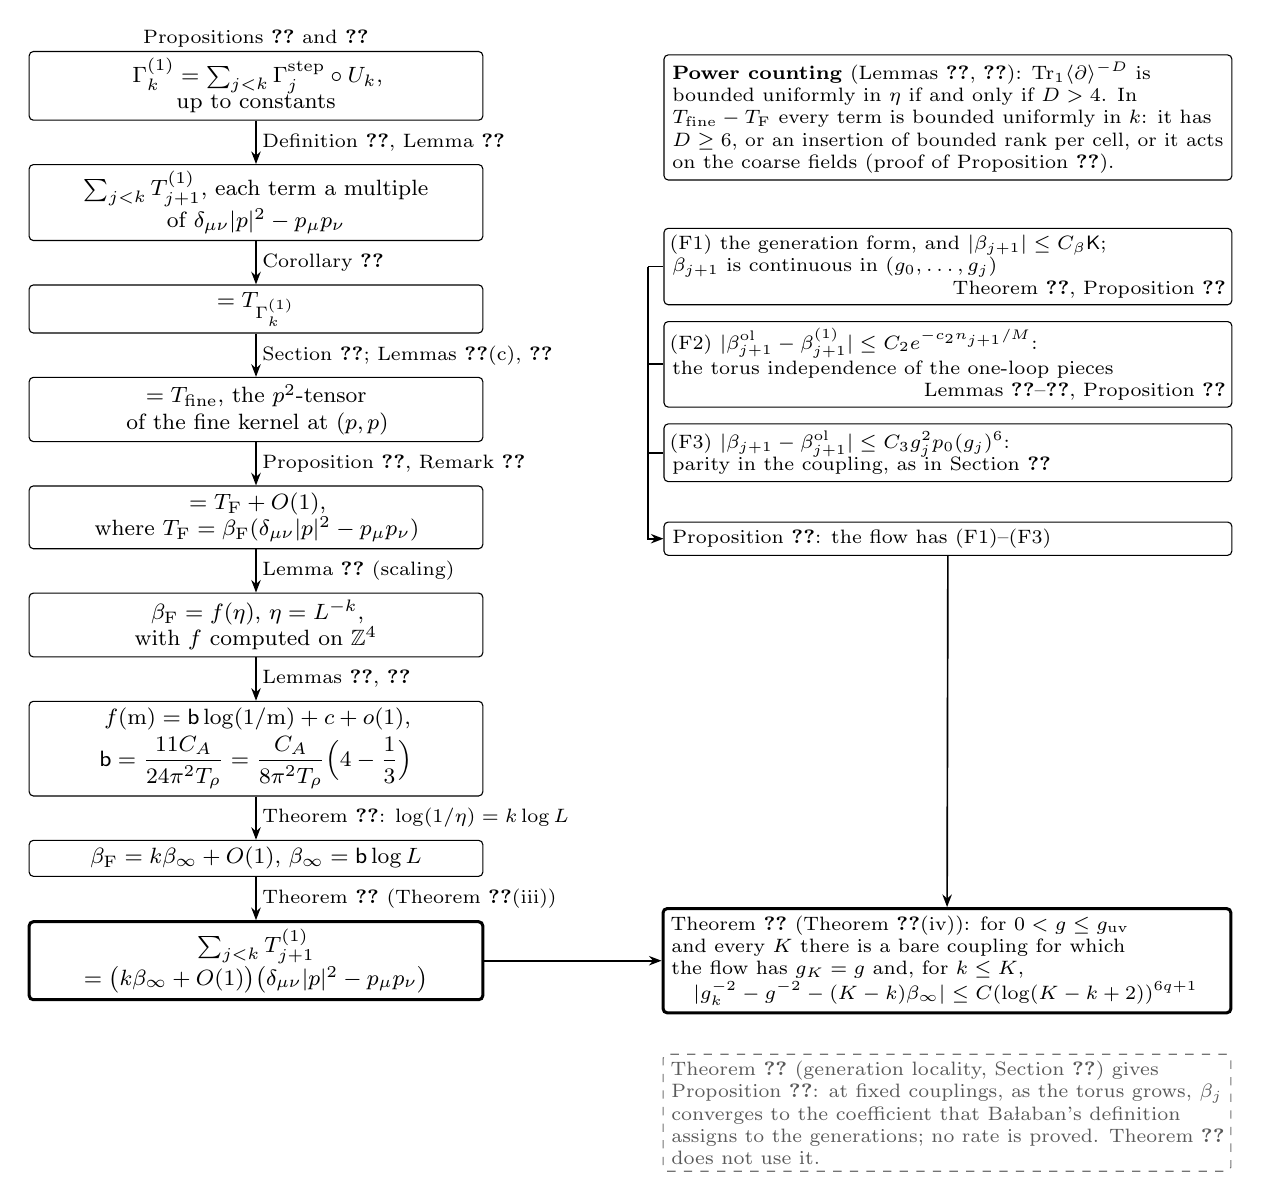
\begin{tikzpicture}[x=1cm,y=1cm,
  ch/.style={draw,rounded corners=1.5pt,fill=white,align=flush center,text width=5.55cm,font=\footnotesize,inner xsep=3pt,inner ysep=2.5pt},
  rc/.style={draw,rounded corners=1.5pt,fill=white,align=flush left,text width=7.0cm,font=\scriptsize,inner xsep=3pt,inner ysep=2.5pt},
  off/.style={rc,dashed,draw=black!55,text=black!65},
  ar/.style={-{Stealth[length=1.6mm]},semithick},
  al/.style={right,font=\scriptsize,inner sep=2pt,align=flush left},
  ]
% the chain of reductions
\node[ch] (b0) at (2.9,0) {$\Gamma^{(1)}_k=\sum_{j<k}\Gamma^{\rm step}_j\circ U_k$,\\ up to constants};
\node[ch,below=5.5mm of b0] (b1) {$\sum_{j<k}T^{(1)}_{j+1}$, each term a multiple\\ of $\delta_{\mu\nu}|p|^2-p_\mu p_\nu$};
\node[ch,below=5.5mm of b1] (b2) {$=T_{\Gamma^{(1)}_k}$};
\node[ch,below=5.5mm of b2] (b3) {$=T_{\rm fine}$, the $p^2$-tensor\\ of the fine kernel at $(p,p)$};
\node[ch,below=5.5mm of b3] (b4) {$=T_{\rm F}+O(1)$,\\ where $T_{\rm F}=\beta_{\rm F}(\delta_{\mu\nu}|p|^2-p_\mu p_\nu)$};
\node[ch,below=5.5mm of b4] (b5) {$\beta_{\rm F}=f(\eta)$, $\eta=L^{-k}$,\\ with $f$ computed on $\Z^4$};
\node[ch,below=5.5mm of b5] (b6) {$f(\mathrm m)=\mathsf b\log(1/\mathrm m)+c+o(1)$,\\[1pt] $\mathsf b=\dfrac{11C_A}{24\pi^2T_\rho}=\dfrac{C_A}{8\pi^2T_\rho}\Big(4-\dfrac13\Big)$};
\node[ch,below=5.5mm of b6] (b7) {$\beta_{\rm F}=k\beta_\infty+O(1)$, $\beta_\infty=\mathsf b\log L$};
\node[ch,below=5.5mm of b7,line width=1.1pt] (b8) {$\sum_{j<k}T^{(1)}_{j+1}$\\ $=\big(k\beta_\infty+O(1)\big)\big(\delta_{\mu\nu}|p|^2-p_\mu p_\nu\big)$};
\draw[ar] (b0) -- node[al] {Definition~\ref{def:marginal-tensor}, Lemma~\ref{lem:ol-symmetry}} (b1);
\draw[ar] (b1) -- node[al] {Corollary~\ref{cor:ol-cumulative}} (b2);
\draw[ar] (b2) -- node[al] {Section~\ref{sec:ol-chart}; Lemmas~\ref{lem:ol-torus-limit}(c), \ref{lem:ol-coarse-map}} (b3);
\draw[ar] (b3) -- node[al] {Proposition~\ref{prop:ol-reduction}, Remark~\ref{rem:ol-symmetry}} (b4);
\draw[ar] (b4) -- node[al] {Lemma~\ref{lem:ol-scaling} (scaling)} (b5);
\draw[ar] (b5) -- node[al] {Lemmas~\ref{lem:ol-infrared}, \ref{lem:ol-classical}} (b6);
\draw[ar] (b6) -- node[al] {Theorem~\ref{thm:ol-log}: $\log(1/\eta)=k\log L$} (b7);
\draw[ar] (b7) -- node[al] {Theorem~\ref{thm:ol-cumulative} (Theorem~\ref{thm:M}(iii))} (b8);
\node[font=\scriptsize,anchor=south,inner sep=1pt] at (b0.north) {Propositions~\ref{prop:ol-laplace} and~\ref{prop:ol-composition}};
% power counting
\node[rc,anchor=north east] (pc) at (15.3,0.4) {\textbf{Power counting} (Lemmas~\ref{lem:ol-integrability}, \ref{lem:ol-power-counting}): $\operatorname{Tr}_1\langle\partial\rangle^{-D}$ is bounded uniformly in $\eta$ if and only if $D>4$. In $T_{\rm fine}-T_{\rm F}$ every term is bounded uniformly in $k$: it has $D\ge6$, or an insertion of bounded rank per cell, or it acts on the coarse fields (proof of Proposition~\ref{prop:ol-reduction}).};
% the ultraviolet limit
\node[rc,below=6mm of pc] (f1) {(F1) the generation form, and $|\beta_{j+1}|\le C_\beta\mathsf K$;\\ $\beta_{j+1}$ is continuous in $(g_0,\dots,g_j)$\\ \mbox{}\hfill Theorem~\ref{thm:sf-flow}, Proposition~\ref{prop:flow-continuity}};
\node[rc,below=2mm of f1] (f2) {(F2) $|\beta^{\rm ol}_{j+1}-\beta^{(1)}_{j+1}|\le C_2e^{-c_2n_{j+1}/M}$:\\ the torus independence of the one-loop pieces\\ \mbox{}\hfill Lemmas~\ref{lem:OL}--\ref{lem:ol-limits}, Proposition~\ref{prop:one-loop-local}};
\node[rc,below=2mm of f2] (f3) {(F3) $|\beta_{j+1}-\beta^{\rm ol}_{j+1}|\le C_3g_j^2p_0(g_j)^6$:\\ parity in the coupling, as in Section~\ref{subsec:cl-order}};
\node[rc,below=5mm of f3] (p6) {Proposition~\ref{prop:flow-F}: the flow has (F1)--(F3)};
\node[rc,line width=1.1pt,anchor=east] (uv) at (15.3,0 |- b8) {Theorem~\ref{thm:ol-uv} (Theorem~\ref{thm:M}(iv)): for $0<g\le g_{\rm uv}$\\ and every $K$ there is a bare coupling for which\\ the flow has $g_K=g$ and, for $k\le K$,\\[1pt] \hspace*{1em}$|g_k^{-2}-g^{-2}-(K-k)\beta_\infty|\le C(\log(K-k+2))^{6q+1}$};
\node[off,below=5mm of uv] (gl) {Theorem~\ref{thm:gen-locality} (generation locality, Section~\ref{sec:gen-locality}) gives Proposition~\ref{prop:beta-identification}: at fixed couplings, as the torus grows, $\beta_j$ converges to the coefficient that Ba\l aban's definition assigns to the generations; no rate is proved. Theorem~\ref{thm:ol-uv} does not use it.};
\foreach \u in {f1,f2,f3} \draw[semithick] ([xshift=-2mm]\u.west) -- (\u.west);
\draw[semithick] ([xshift=-2mm]f1.west) -- ([xshift=-2mm]f3.west);
\draw[ar] ([xshift=-2mm]f3.west) |- (p6.west);
\draw[ar] (p6) -- (uv);
\draw[ar] (b8) -- (uv);
\end{tikzpicture}
\caption{Part~XI: the chain of reductions to the one-loop coefficient (left) and the ultraviolet limit (right). Left: each arrow carries the results that give the next line; together they are Theorem~\ref{thm:ol-cumulative}, which is Theorem~\ref{thm:M}(iii), with $O(1)$ bounded uniformly in $k$. The marginal tensors have no term linear in $p$ (Lemma~\ref{lem:ol-symmetry}). The coefficient is $\mathsf b=\frac{11C_A}{24\pi^2T_\rho}$; in Lemma~\ref{lem:ol-classical} the factor $4-\frac13=\frac{11}3$ is the sum of the spin part $4$ and the orbital part $-\frac13$, which is $+\frac13$ from the scalar determinant and $-\frac23$ from the vector determinant. Right: the properties (F1)--(F3) of the flow (Section~\ref{subsec:ol-flow-coeff}), proved in Proposition~\ref{prop:flow-F}, and Theorem~\ref{thm:M}(iii) give Theorem~\ref{thm:M}(iv), under the conditions on $\gamma$ stated there; for the last $m_1$ steps see the paragraph after Theorem~\ref{thm:ol-uv}. Dashed: off the line of Theorem~\ref{thm:M}(iv).}
\label{fig:G-partXI}
\end{gfigure}


\paragraph{Normalization.} The action is $S=\sum_p(\mathsf N-\frac12\operatorname{tr}(U(\partial p)+U(\partial p)^{-1}))$ (Section~\ref{sec:action}), with the trace of a representation $\rho$, $\operatorname{tr}_\rho(T^aT^b)=T_\rho\delta^{ab}$ (Theorem~\ref{thm:M}). Its continuum limit is $\frac{T_\rho}4\sum_{\mu\nu}F^a_{\mu\nu}F^a_{\mu\nu}$ (Remark~\ref{rem:ol-heat-kernel}). So $g^{-2}S$ corresponds to the standard $\frac1{4g_{\rm std}^2}\sum F^aF^a$ with
\[
g_{\rm std}^2=g^2/T_\rho .
\]
The coefficient is $\mathsf b=\frac{11C_A}{24\pi^2T_\rho}$ and $\beta_\infty=\mathsf b\log L$ (Theorem~\ref{thm:ol-log}); along the flow, $g_k^{-2}-g_K^{-2}=(K-k)\beta_\infty$ up to the error of Theorem~\ref{thm:ol-uv}. For $SU(N)$ in the fundamental representation, $T_\rho=\frac12$ and $\beta_\infty=\frac{11N}{12\pi^2}\log L$. In Theorem~\ref{thm:ol-uv}, $g$ is the coupling of the last scale and $g_0$ the bare coupling (Section~\ref{subsec:ol-flow-coeff}).

\paragraph{The chain of reductions (Sections~\ref{sec:ol-composite}--\ref{sec:ol-feynman}).}
\begin{itemize}
\item \emph{The composite one-loop term.} $\Gamma^{(1)}_k(V)$ is defined by Laplace's method on the fibre of the fine configurations with averages $V$, near the minimal orbit (Proposition~\ref{prop:ol-laplace}). Integrating the fibre scale by scale gives $\Gamma^{(1)}_k(V)=\sum_{j<k}\Gamma^{\rm step}_j(U_k(V))$ up to constants (Lemma~\ref{lem:ol-one-step}, Proposition~\ref{prop:ol-composition}).
\item \emph{Exact symmetry.} $\Gamma^{(1)}_k$ and the step functions $V'\mapsto\Gamma^{\rm step}_j(U_{j+1}(V'))$ are invariant under the translations and under $B_4$. So their marginal tensors, the parts of order $p^2$ of their vacuum polarizations in infinite volume, are $\beta(\delta_{\mu\nu}|p|^2-p_\mu p_\nu)$ with a single coefficient, and there is no term linear in $p$ (Lemma~\ref{lem:ol-symmetry}). The symmetry comes from Ba\l aban's symmetric averaging, the Haar measure and the covariance of the minimal orbits (the paragraph after Theorem~\ref{thm:M}); a linear term would produce relevant terms of order $1$ in every step (Remark~\ref{rem:marginal-orders}).
\item \emph{Infinite volume and the change of scale.} The operators at $U=1$ are constructed in infinite volume by folding the operators on the tori (Section~\ref{subsec:ol-infinite-volume}). In four dimensions the change of scale leaves marginal tensors unchanged (Lemma~\ref{lem:ol-pullback}). Hence $\sum_{j<k}T^{(1)}_{j+1}=T_{\Gamma^{(1)}_k}$ (Corollary~\ref{cor:ol-cumulative}).
\item \emph{The Landau chart.} Up to a constant, $\Gamma^{(1)}_k(V)=-\frac12\log\det\bL_*-\frac12\log\det(\bQ_k\bG_*\bQ_k^T)$ plus the logarithm of a ghost determinant, at the background $U_0=U_k(V)$, where $\bL_*=q_2+D_{U_0}RD^T_{U_0}+a\bQ_k^T\bQ_k$ is built from the Hessian form $q_2$ of Proposition~\ref{prop:hessian} and $\bG_*=\bL_*^{-1}$ (Theorem~\ref{thm:ol-chart}, Corollary~\ref{cor:ol-ghost}). Its marginal tensor is the $p^2$-tensor $T_{\rm fine}$ of a fine-lattice vacuum polarization at $U=1$ (Lemma~\ref{lem:ol-coarse-map}).
\item \emph{Reduction to the Feynman gauge.} The vector and ghost operators are compared with the lattice operators of the background Feynman gauge with mass $1$. Power counting with the weights $\langle\partial\rangle$ bounds the trace per cell of every product of degree $D>4$, and of every product with a factor of finite rank per cell, uniformly in $\eta$ (Lemmas~\ref{lem:ol-power-counting} and~\ref{lem:ol-remainders}). Hence $T_{\rm fine}=T_{\rm F}+O(1)$ uniformly in $k$, where $T_{\rm F}$ is the tensor of the Feynman-gauge one-loop term (Proposition~\ref{prop:ol-reduction}).
\item \emph{The lattice integral.} By scaling, the isotropic coefficient of $T_{\rm F}$ is $\beta_{\rm F}=f(\eta)$, the $p^2$-coefficient on $\Z^4$ with mass $\eta$ (Lemma~\ref{lem:ol-scaling}). As $\mathrm m\to0$, $f(\mathrm m)=\mathsf b\log(1/\mathrm m)+c+o(1)$ (Lemma~\ref{lem:ol-infrared}). The coefficient comes from the spherical average of the continuum Feynman-gauge integrand (Lemma~\ref{lem:ol-classical} and its proof):
\[
\mathsf b=\frac{C_A}{8\pi^2T_\rho}\Big(4-\frac13\Big)=\frac{11C_A}{24\pi^2T_\rho},
\]
with the spin part $4$ and the orbital part $-\frac13$, itself $+\frac13$ from the scalar determinant and $-\frac23$ from the vector determinant. Since $\log(1/\eta)=k\log L$, $\beta_{\rm F}=k\beta_\infty+O(1)$ (Theorem~\ref{thm:ol-log}).
\end{itemize}
Together: $\sum_{j<k}T^{(1)}_{j+1}=(k\beta_\infty+O(1))(\delta_{\mu\nu}|p|^2-p_\mu p_\nu)$, uniformly in $k$ (Theorem~\ref{thm:ol-cumulative}).

\paragraph{Transfer to the flow (Section~\ref{sec:ol-uv}).} The flow reads $\beta_{j+1}$ off on the torus; Part~XI computes $\beta^{(1)}_{j+1}$ in infinite volume. Three properties of the flow connect them, all proved in Proposition~\ref{prop:flow-F} under ($\Gamma$1)--($\Gamma$4).
\begin{itemize}
\item[(F1)] The densities have the generation form, and $\beta_{j+1}$ is a continuous function of $(g_0,\dots,g_j)$ with $|\beta_{j+1}|\le C_\beta\mathsf K$ (Proposition~\ref{prop:flow-continuity}).
\item[(F2)] The one-loop part $\beta^{\rm ol}_{j+1}$ of $\beta_{j+1}$ differs from $\beta^{(1)}_{j+1}$ by at most $C_2e^{-c_2n_{j+1}/M}$. This rests on the torus independence of the one-loop pieces (Proposition~\ref{prop:one-loop-local}, Lemma~\ref{lem:OL}) and on the infinite-volume limits of the second variations (Lemma~\ref{lem:ol-limits}). These errors are summable over the scales (Remark~\ref{rem:flow-F}(b)).
\item[(F3)] The rest is $|\beta_{j+1}-\beta^{\rm ol}_{j+1}|\le C_3g_j^2p_0(g_j)^6$, by parity in the coupling and Cauchy's estimate. Without parity it would be of order $gp_0^3$, which is not summable along the flow (Remark~\ref{rem:flow-F}(b)).
\end{itemize}

\paragraph{The exit argument and Theorem~\ref{thm:ol-uv}.} The set of bare couplings $g_0$ for which $g_1,\dots,g_K$ stay in $(0,\gamma]$ is closed and contains a small interval, and $g_0\mapsto g_K$ is continuous on it (Corollary~\ref{cor:bare-continuity}). At the end of its first component some $g_j$ equals $\gamma$, and the lower bound from (F2) and (F3) forces $g_K$ above a fixed number; the intermediate value theorem gives $g_0$ with $g_K=g$ (proof of Theorem~\ref{thm:ol-uv}). With $p_0(g)=(\log g^{-1})^q$ and $\gamma$ subject to ($\Gamma$1)--($\Gamma$4), $\gamma\le e^{-3q}$ and $C_3\gamma^2p_0(\gamma)^6\le\frac12\beta_\infty$, Theorem~\ref{thm:ol-uv} states: there are $g_{\rm uv}>0$ and $C$, independent of $K$ and of the torus, such that for $0<g\le g_{\rm uv}$ and every $K$ some bare coupling gives $g_k\in(0,\gamma]$ for $k\le K$, $g_K=g$, and
\[
\Big|\frac1{g_k^2}-\frac1{g^2}-(K-k)\beta_\infty\Big|\le C\big(\log(K-k+2)\big)^{6q+1}\qquad(k\le K).
\]
For $K-k\ge m_1$, with $m_1$ independent of $K$, $g$ and the torus, this is the analogue of Ba\l aban's (0.31) for the couplings of the small-field flow. For the last $m_1$ steps it gives the upper half, and the lower half up to an additive constant (the paragraph after Theorem~\ref{thm:ol-uv}, Remark~\ref{rem:ol-remains}(c)). The theorem concerns the small-field model (Remark~\ref{rem:ol-remains}(a)).

\paragraph{Generation locality (Section~\ref{sec:gen-locality}).} For polymers that do not wrap, and at flat configurations, the new terms of a step are a single functional, defined on the infinite lattice, of the old activities (Proposition~\ref{prop:gl-functional}). By induction over the scales, at fixed couplings the generations converge as the torus grows, and so do the coefficients (Theorem~\ref{thm:gen-locality}). Hence $\beta_j$ converges to the coefficient that Ba\l aban's definition \cite[(1.20)--(1.22)]{BalYM4I} assigns to the generations of this note (Proposition~\ref{prop:beta-identification}). No rate is proved. This line is not used by Theorem~\ref{thm:ol-uv}.

\paragraph{The $\beta$'s and the $T$'s.} Table~\ref{tab:G-betas} lists the coefficients and tensors of Part~XI and of the flow.

\begin{table}[htbp]
\centering\small
\renewcommand{\arraystretch}{1.2}
\begin{tabular}{@{}p{0.17\textwidth}p{0.53\textwidth}p{0.22\textwidth}@{}}
\hline
\raggedright Symbol & \raggedright Meaning & \raggedright Where \tabularnewline
\hline
\raggedright $\beta_j=\beta_{E^{(j)}}$ & \raggedright coefficient of the generation $E^{(j)}$, read off from its period density on the torus; $g_j^{-2}=g_{j-1}^{-2}-\beta_j$ & \raggedright Proposition~\ref{prop:period-iso}, Theorem~\ref{thm:sf-flow} \tabularnewline
\raggedright $\beta^{\rm ol}_{j+1}$ & \raggedright one-loop part of $\beta_{j+1}$, through the volume coefficient \eqref{eq:beta-vol}; independent of the couplings & \raggedright Section~\ref{subsec:ol-flow-coeff} \tabularnewline
\raggedright $\beta^{(1)}_{j+1}$ & \raggedright coefficient of $T^{(1)}_{j+1}$, in infinite volume & \raggedright Theorem~\ref{thm:ol-cumulative} \tabularnewline
\raggedright $\beta_{\rm F}$ & \raggedright isotropic coefficient of $T_{\rm F}$; $\beta_{\rm F}=f(\eta)$ & \raggedright Theorem~\ref{thm:ol-log}, Lemma~\ref{lem:ol-scaling} \tabularnewline
\raggedright $\mathsf b$, $\beta_\infty$ & \raggedright $\mathsf b=\frac{11C_A}{24\pi^2T_\rho}$, $\beta_\infty=\mathsf b\log L$ & \raggedright Lemma~\ref{lem:ol-classical}, Theorem~\ref{thm:ol-log} \tabularnewline
\raggedright $\beta^{\rm B}_j$, $\beta^\infty_j$ & \raggedright Ba\l aban's coefficient of the generations of this note, the limit of $\beta_j$ as the torus grows & \raggedright Proposition~\ref{prop:beta-identification}, Theorem~\ref{thm:gen-locality} \tabularnewline
\raggedright $T_\Phi$; $T^{(1)}_{j+1}$, $T_{\Gamma^{(1)}_k}$ & \raggedright marginal tensor of a function $\Phi$, the $p^2$-part of its vacuum polarization; those of the step functions and of the composite one-loop term & \raggedright Definition~\ref{def:marginal-tensor}, Corollary~\ref{cor:ol-cumulative} \tabularnewline
\raggedright $T_{\rm fine}$, $T_{\rm F}$ & \raggedright $p^2$-tensors at $U=1$ of the fine-lattice one-loop term and of its Feynman-gauge counterpart & \raggedright Lemma~\ref{lem:ol-coarse-map}, Proposition~\ref{prop:ol-reduction} \tabularnewline
\raggedright $\bar T_E$, $\bar T_S$ & \raggedright period densities: quadratic forms in a constant curvature & \raggedright Definition~\ref{def:period-density} \tabularnewline
\raggedright $T_\rho$ & \raggedright a number, the normalization of the trace: $\operatorname{tr}_\rho(T^aT^b)=T_\rho\delta^{ab}$ & \raggedright Theorem~\ref{thm:M} \tabularnewline
\hline
\end{tabular}
\caption{Coefficients and tensors of the flow and of Part~XI.}\label{tab:G-betas}
\end{table}

\paragraph{Where in the note.} Section~\ref{sec:ol-composite}: composition, symmetry, infinite volume, change of scale. Section~\ref{sec:ol-chart}: the Landau chart. Section~\ref{sec:ol-vacpol}: reduction to the Feynman gauge. Section~\ref{sec:ol-feynman}: the lattice integral and the coefficient $\mathsf b$. Section~\ref{sec:ol-uv}: (F1)--(F3) and the ultraviolet limit. Section~\ref{sec:gen-locality}: generation locality.

\paragraph{In the companion.} The chapters on the first and on the second half of Part~XI.

% A guide to the proof, Sections G11--G14 (readability layer). Unnumbered: no numbered sections,
% theorems or displays. Every informal statement cites the result it paraphrases.
\gsection{The order of the parameters}\label{g:parameters}

% Figure of the guide (G11): the order in which the parameters are chosen. Owner: WP7.
\begin{gfigure}[tp]
\centering
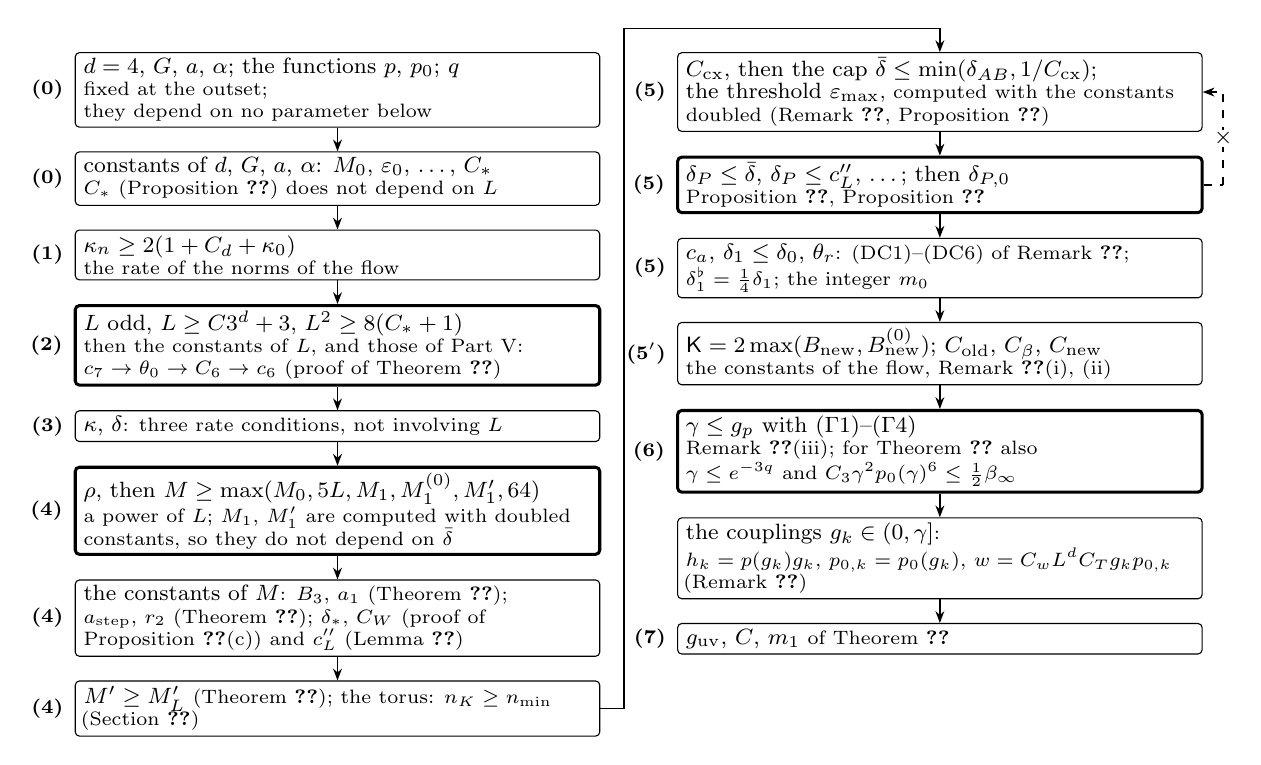
\begin{tikzpicture}[x=1cm,y=1cm,
  pm/.style={draw,rounded corners=1.5pt,fill=white,align=flush left,text width=6.45cm,font=\scriptsize,inner xsep=3pt,inner ysep=2pt},
  key/.style={pm,line width=1.1pt},
  tg/.style={anchor=east,font=\scriptsize\bfseries,inner sep=1pt},
  ar/.style={-{Stealth[length=1.5mm]},semithick},
  ]
\def\P#1{{\footnotesize #1}}
% left column: up to M'
\node[pm,anchor=north west] (l0) at (0.75,0) {\P{$d=4$, $G$, $a$, $\alpha$; the functions $p$, $p_0$; $q$}\\ fixed at the outset;\\ they depend on no parameter below};
\node[pm,below=3mm of l0] (l1) {\P{constants of $d$, $G$, $a$, $\alpha$: $M_0$, $\eps_0$, \dots, $C_*$}\\ $C_*$ (Proposition~\ref{prop:sharp-curvature}) does not depend on $L$};
\node[pm,below=3mm of l1] (l2) {\P{$\kappa_n\ge2(1+C_d+\kappa_0)$}\\ the rate of the norms of the flow};
\node[key,below=3mm of l2] (l3) {\P{$L$ odd, $L\ge C3^d+3$, $L^2\ge8(C_*+1)$}\\ then the constants of $L$, and those of Part~V:\\ $c_7\to\theta_0\to C_6\to c_6$ (proof of Theorem~\ref{thm:variational})};
\node[pm,below=3mm of l3] (l4) {\P{$\kappa$, $\delta$}: three rate conditions, not involving $L$};
\node[key,below=3mm of l4] (l5) {\P{$\rho$, then $M\ge\max(M_0,5L,M_1,M^{(0)}_1,M'_1,64)$}\\ a power of $L$; $M_1$, $M'_1$ are computed with doubled\\ constants, so they do not depend on $\bar\delta$};
\node[pm,below=3mm of l5] (l6) {\P{the constants of $M$}: $B_3$, $a_1$ (Theorem~\ref{thm:balaban});\\ $a_{\rm step}$, $r_2$ (Theorem~\ref{thm:step}); $\delta_*$, $C_W$ (proof of\\ Proposition~\ref{prop:dirichlet-hessian}(c)) and $c''_L$ (Lemma~\ref{lem:coercive-general})};
\node[pm,below=3mm of l6] (l7) {\P{$M'\ge M'_L$} (Theorem~\ref{thm:step-coercive}); the torus: $n_K\ge n_{\min}$\\ (Section~\ref{subsec:tf-scales})};
% right column: the domains, the flow constants, the couplings
\node[pm,anchor=north west] (r0) at (8.4,0) {\P{$C_{\rm cx}$, then the cap $\bar\delta\le\min(\delta_{AB},1/C_{\rm cx})$;}\\ \P{the threshold $\eps_{\max}$}, computed with the constants\\ doubled (Remark~\ref{rem:domain-constants}, Proposition~\ref{prop:complex-ext})};
\node[key,below=3mm of r0] (r1) {\P{$\delta_P\le\bar\delta$, $\delta_P\le c''_L$, \dots; then $\delta_{P,0}$}\\ Proposition~\ref{prop:complex-ext}, Proposition~\ref{prop:first-step}};
\node[pm,below=3mm of r1] (r2) {\P{$c_a$, $\delta_1\le\delta_0$, $\theta_r$}: (DC1)--(DC6) of Remark~\ref{rem:domain-constants};\\ $\delta_1^\flat=\frac14\delta_1$; the integer $m_0$};
\node[pm,below=3mm of r2] (r3) {\P{$\mathsf K=2\max(B_{\rm new},B^{(0)}_{\rm new})$; $C_{\rm old}$, $C_\beta$, $C_{\rm new}$}\\ the constants of the flow, Remark~\ref{rem:flow-constants}(i), (ii)};
\node[key,below=3mm of r3] (r4) {\P{$\gamma\le g_p$ with ($\Gamma$1)--($\Gamma$4)}\\ Remark~\ref{rem:flow-constants}(iii); for Theorem~\ref{thm:ol-uv} also\\ $\gamma\le e^{-3q}$ and $C_3\gamma^2p_0(\gamma)^6\le\frac12\beta_\infty$};
\node[pm,below=3mm of r4] (r5) {\P{the couplings $g_k\in(0,\gamma]$}:\\ $h_k=p(g_k)g_k$, $p_{0,k}=p_0(g_k)$, $w=C_wL^dC_Tg_kp_{0,k}$\\ (Remark~\ref{rem:flow-constants})};
\node[pm,below=3mm of r5] (r6) {\P{$g_{\rm uv}$, $C$, $m_1$} of Theorem~\ref{thm:ol-uv}};
% tags: the items of Remark 49.8
\foreach \n/\t in {l0/(0),l1/(0),l2/(1),l3/(2),l4/(3),l5/(4),l6/(4),l7/(4),r0/(5),r1/(5),r2/(5),r3/(5$'$),r4/(6),r6/(7)}
  \node[tg] at ([xshift=-1mm]\n.west) {\t};
% the order
\foreach \u/\v in {l0/l1,l1/l2,l2/l3,l3/l4,l4/l5,l5/l6,l6/l7,r0/r1,r1/r2,r2/r3,r3/r4,r4/r5,r5/r6} \draw[ar] (\u) -- (\v);
\draw[ar] (l7.east) -- ++(0.3,0) |- ([yshift=3mm]r0.north) -- (r0.north);
% no dependence of eps_max on delta_P
\draw[dashed,semithick] (r1.east) -- ++(0.25,0) coordinate (xa);
\draw[ar,dashed] (xa) -- (xa |- r0.east) -- (r0.east);
\node[fill=white,inner sep=0.3pt,font=\footnotesize] at ($(xa)!0.5!(xa |- r0.east)$) {$\times$};
\end{tikzpicture}
\caption{The order in which the parameters are chosen. Each box may depend on the boxes before it, in the order of the arrows: the left column, then the right one (Remark~\ref{rem:parameters}). A tag is the stage of the box: (1)--(6) are the items of Remark~\ref{rem:parameters}, (0) the data fixed at the outset and their constants, (5$'$) the constants of the flow, which Remark~\ref{rem:flow-constants} places between items~(5) and~(6), and (7) the constants of Theorem~\ref{thm:ol-uv}. Thick frames: the block size $L$, the scale $M$, the size $\delta_P$ of the complex references, and the bound $\gamma$ on the couplings. The radius $\delta_*$ and the constant $C_W$ are fixed in the proof of Proposition~\ref{prop:dirichlet-hessian}(c), and $c''_L$ with $C_{\rm cmp}c''_L\le\delta_*$ in the proof of Lemma~\ref{lem:coercive-general}; they depend on $M$, and $\delta_P\le c''_L$ (Proposition~\ref{prop:complex-ext}). Crossed dashed arrow: $\eps_{\max}$ does not depend on $\delta_P$, since its thresholds are computed with every multiplicative constant doubled (Remark~\ref{rem:domain-constants}). Every condition on $\gamma$ is an upper bound by quantities fixed before it, so the order has no cycle (Remark~\ref{rem:parameters}(6)).}
\label{fig:G-parameters}
\end{gfigure}


The parameters of Parts~VII--XI are chosen in a fixed order, and each may depend only on those chosen before it (Remark~\ref{rem:parameters}). The order is stated in Remark~\ref{rem:parameters}, completed by Remarks~\ref{rem:domain-constants}, \ref{rem:step-M} and~\ref{rem:flow-constants}, and, for the constants of Parts~V and~VI, by the proofs of Theorems~\ref{thm:variational} and~\ref{thm:balaban}. The parameter ledger of the companion collects the constants with their dependencies; Table~\ref{tab:G-parameters} follows it, and Figure~\ref{fig:G-parameters} shows the chain. Three facts make the order acyclic.
\begin{itemize}
\item Every lower bound on $M$ uses only quantities fixed before $M$ (Remark~\ref{rem:parameters}(4)). Several constants of Part~VII do not depend on $M$ (Remark~\ref{rem:step-M}).
\item The domain constants are fixed after $M$ and $M'$, and the cap $\bar\delta$ on the size of the complex references comes before the threshold $\eps_{\max}$ and the radius $\delta_P$ (Remark~\ref{rem:domain-constants}).
\item Every condition on $\gamma$ is an upper bound by quantities fixed before $\gamma$, and remains true when $\gamma$ decreases (Remark~\ref{rem:parameters}(6)). The constants of the flow do not depend on the couplings or on the torus (Theorem~\ref{thm:sf-flow}).
\end{itemize}
The torus satisfies (T0)--(T2) at every scale once $n_K\ge n_{\min}$ and $\ell L^N$ is a power of $L$, and $n_{\min}$ depends on the parameters up to stage~(4) (Remark~\ref{rem:parameters}, Section~\ref{subsec:tf-scales}).

\begin{table}[tbp]
\centering\small
\renewcommand{\arraystretch}{1.15}
\begin{tabular}{|p{0.06\textwidth}|p{0.33\textwidth}|p{0.33\textwidth}|p{0.16\textwidth}|}
\hline
Stage & Parameters and their role & Main conditions & Fixed in\tabularnewline
\hline
(0) & \raggedright $d=4$; the group $G$; the averaging coefficient $a$; the H\"older exponent $\alpha$; the functions $p$, $p_0$ and, in Theorem~\ref{thm:ol-uv}, the exponent $q$. Then the constants of Parts~I--III that do not depend on $L$ or $M$ (Remark~\ref{rem:uniformity-limits}(b)) and of the interior estimates, among them $M_0$, and $C_*$ & \raggedright $\alpha\le\frac12$ from Section~\ref{sec:weak-background} on; $C_*$ does not depend on $L$ & \raggedright \S\ref{subsec:flow-parameters}, Thm.~\ref{thm:reg-coercive}, Prop.~\ref{prop:sharp-curvature}\tabularnewline
(1) & \raggedright the rate $\kappa_n$ of the activity norms, after the constants $\kappa_0$, $K_0$ of $d_M$ and $C_d$ of the polymer expansion & \raggedright $\kappa_n\ge2(1+C_d+\kappa_0)$ & \raggedright Rem.~\ref{rem:parameters}(1)\tabularnewline
(2) & \raggedright the block factor $L$, odd. Then the constants of $L$ alone, among them $c_L$ and $\beta_\infty$; the constants of Part~V ($\theta_0$, $c_6$, $C_6$, $\gamma'$); the constants of Part~VII that do not depend on $M$ ($C_L$, $c'_L$) & \raggedright $L\ge C3^d+3$ (reblocking); $L^2\ge8(C_*+1)$ (thresholds of consecutive steps) & \raggedright Rem.~\ref{rem:parameters}(2), Thm.~\ref{thm:variational}, Rem.~\ref{rem:step-M}\tabularnewline
(3) & \raggedright the weakening rate $\kappa$ and the loss $\delta$ of Part~IX; $\kappa'_w=\kappa-C\delta$ and $\kappa_2=3^{-d}\kappa'_w$ & \raggedright three rate conditions, which make every source decay at the rate $\kappa_n$ after reblocking & \raggedright Rem.~\ref{rem:parameters}(3)\tabularnewline
(4) & \raggedright $\rho$; the thresholds $M_1$, $M_1^{(0)}$, $M'_1$; the grid size $M$. Then the constants of $M$: $a_1$, $B_3$, $a_2$, $B_5$, $a_\delta$, $r_2$, $a_{\rm step}$, the constants of Theorem~\ref{thm:weak-bg}; then $\delta_*$, $C_W$, and $c''_L$. Then the scale $M'$ of the step; then $n_*$, $n_{\min}$ & \raggedright $M>32(L+1)$, a power of $L$, $M\ge\max(M_0,5L,M_1,M_1^{(0)},M'_1,64)$, $M\ge16r$; $C_{\rm AB}c''_L\le c'_L$, $C_{\rm cmp}c''_L\le\delta_*$; $M'\ge M'_L$; (T0)--(T2) & \raggedright Rem.~\ref{rem:parameters}(4), Thm.~\ref{thm:balaban}, proofs of Prop.~\ref{prop:dirichlet-hessian}(c) and Lemma~\ref{lem:coercive-general}, \S\ref{subsec:tf-scales}\tabularnewline
(5) & \raggedright the domain constants: the cap $\bar\delta$, the threshold $\eps_{\max}$, the radii $\delta_P$, $\delta_{P,0}$ of the complex references, $c_a$, $\delta_1\le\delta_0$, $\theta_r$; $\delta_1^\flat=\frac14\delta_1$; then $m_0$; the constants of the step quantities & \raggedright $\bar\delta\le\min(\delta_{AB},1/C_{\rm cx})$; $\delta_P\le\bar\delta$, $\delta_P\le c''_L$; (DC1)--(DC6) & \raggedright Rem.~\ref{rem:domain-constants}, Rem.~\ref{rem:parameters}(5), Prop.~\ref{prop:complex-ext}\tabularnewline
(5$'$) & \raggedright the constants of the flow: $B_{\rm new}$, $B_{\rm new}^{(0)}$, then $\mathsf K=2\max(B_{\rm new},B^{(0)}_{\rm new})$; $C_{\rm old}$, $C_\beta$, $C_{\rm ex}$, $C_{\rm new}$, $C^{(0)}_{\rm new}$; $c_{\rm F}$; $C_2$, $C_3$ of (F2), (F3) & \raggedright none; they do not depend on the couplings or the torus & \raggedright Rem.~\ref{rem:flow-constants}(i),(ii), Prop.~\ref{prop:flow-F}\tabularnewline
(6) & \raggedright the bound $\gamma\le g_p$ on the couplings & \raggedright ($\Gamma$1)--($\Gamma$4); for Theorem~\ref{thm:ol-uv} also $\gamma\le e^{-3q}$ and $C_3\gamma^2p_0(\gamma)^6\le\frac12\beta_\infty$ & \raggedright Rem.~\ref{rem:parameters}(6), Rem.~\ref{rem:flow-constants}\tabularnewline
(7) & \raggedright $g_{\rm uv}$, $C$ and $m_1$ of the ultraviolet limit & \raggedright $g_{\rm uv}$ small & \raggedright Thm.~\ref{thm:ol-uv}\tabularnewline
\hline
\end{tabular}
\caption{The order of the parameters. Stage (5$'$) lies between stages (5) and (6) of Remark~\ref{rem:parameters}. The constants $\delta_*$, $C_W$ and $c''_L$ depend on $M$ and are fixed after it (proofs of Proposition~\ref{prop:dirichlet-hessian}(c) and Lemma~\ref{lem:coercive-general}); $c''_L$ enters the choice of $\delta_P$ (Proposition~\ref{prop:complex-ext}).}\label{tab:G-parameters}
\end{table}

\paragraph{The named constants.} The constants that recur in the statements are the following.
\begin{itemize}
\item $a_1$, $B_3$: background fields exist for real coarse configurations of curvature at most $\eps_1\le a_1$, and they have curvature and current at most $B_3\eps_1$ (Theorem~\ref{thm:balaban}).
\item $C_*$: the curvature of a background field is at most $(C_*+\delta)$ times that of the coarse configuration, with $C_*$ independent of $L$ (Proposition~\ref{prop:sharp-curvature}). Hence the condition $L^2\ge8(C_*+1)$.
\item $\theta_0$, $c_6$, $C_6$: the class $\mathfrak U(\theta_0)$ of configurations of small curvature and current in which the critical orbit is unique, the threshold $\eps+\beta\le c_6$ on the reference and the data, and the constant of the bounds (Theorem~\ref{thm:variational}).
\item $a_{\rm step}$, $r_2$, $c_L$: the curvature threshold of the coarse configuration and the bound on the fluctuation cutoff in Theorem~\ref{thm:K}, and the coercivity constant of the step, from a Poincar\'e inequality for one step (Theorem~\ref{thm:K}(ii), Lemma~\ref{lem:poincare-step}).
\item $h_k=p(g_k)g_k$, $w$, $p_0$: the three cutoffs of the small-field step (Table~\ref{tab:G-cutoffs}).
\item $\kappa_2$: the decay rate of the one-loop pieces, $|\mathfrak e(X)|\le Ce^{-(\kappa_2-1)|X|}$ (Proposition~\ref{prop:one-loop-polymer}).
\item $\mathsf K$, $C_\beta$, $C_{\rm old}$: the bound of every generation, the bound $|\beta_j|\le C_\beta\mathsf K$, and the bound $C_{\rm old}\mathsf K$ of the old activities (Theorem~\ref{thm:N}, Proposition~\ref{prop:old-activities}).
\item $m_0$: the age after which the marginal part of a generation is extracted (Definition~\ref{def:polymer-classes}); $m_1$: the number of last steps for which Theorem~\ref{thm:ol-uv} gives the lower half of the analogue of (0.31) only up to a constant.
\end{itemize}

\paragraph{Where in the note.} Remarks~\ref{rem:parameters}, \ref{rem:domain-constants}, \ref{rem:step-M} and~\ref{rem:flow-constants}; the proofs of Theorems~\ref{thm:variational} and~\ref{thm:balaban}; Section~\ref{subsec:tf-scales}.

\paragraph{In the companion.} The chapter on the parameter ledger. Its tables list the constants of Parts~VII--XI, and those of Parts~I--VI that these Parts use, with their definitions, dependencies, conditions and uses, and it checks that the order has no cycle.

\gsection{Notation}\label{g:notation}

The notation index is Appendix~\ref{app:notation}. It lists the symbols used across several Parts with their meanings and the places of their definitions. Letters with several meanings are listed with all of them, and the index says how the meanings are kept apart. Appendix~\ref{app:notation} also lists the named conditions, such as (A1)--(A11), (L1)--(L5), (DC1)--(DC6) and ($\Gamma$1)--($\Gamma$4), and the operators, and it gives the former names of the renamed symbols. Remark~\ref{rem:notation-flow} collects the notation of Sections~\ref{sec:step-quantities}--\ref{sec:flow4}.

\gsection{Comparison with Ba\l aban and Dimock}\label{g:comparison}

The note follows Ba\l aban's renormalization group for four-dimensional lattice Yang--Mills theory \cite{BalPropI,BalPropII,BalAvg,BalReg,BalBackground,BalVar,BalYM4I,BalYM4II}, and, for the small-field step in polymer form, Dimock's account of Ba\l aban's method \cite{DimockI}. Table~\ref{tab:G-comparison} lists where it follows them and where it differs. The comparison is restricted to what the note states about these papers.

\begin{table}[tbp]
\centering\footnotesize
\renewcommand{\arraystretch}{1.0}\setlength{\tabcolsep}{4pt}
\begin{tabular}{|p{0.15\textwidth}|p{0.32\textwidth}|p{0.31\textwidth}|p{0.14\textwidth}|}
\hline
Item & Ba\l aban, Dimock & This note & Where\tabularnewline
\hline
\raggedright coercivity at $U=1$ & \raggedright momentum space \cite{BalPropI} & \raggedright position space; one Fourier lower bound & \raggedright Thm.~\ref{thm:gauge-coercive}, Cor.~\ref{cor:QKQ-lower}\tabularnewline
\raggedright positivity at regular backgrounds & \raggedright \cite[Theorem~3.11]{BalBackground} and local axial-gauge estimates \cite[Lemma~2.4]{BalPropII} & \raggedright IMS localization and the coercivity of Part~I & \raggedright Thm.~\ref{thm:reg-coercive}, \S\ref{sec:outlook}\tabularnewline
\raggedright Dirichlet operators & \raggedright Dirichlet operators on domains \cite{BalBackground} & \raggedright a mass term near the boundary (\S\ref{sec:outlook}); in the note, Dirichlet conditions for all components (Rem.~\ref{rem:L3-domains}) & \raggedright Thm.~\ref{thm:G}(ii), Rem.~\ref{rem:L3-domains}\tabularnewline
\raggedright averaging & \raggedright symmetric averaging \cite[(0.3)--(0.12)]{BalYM4I} & \raggedright the same; its linearization has $E=0$ & \raggedright \S\ref{sec:averaging}, Cor.~\ref{cor:parts-apply}\tabularnewline
\raggedright axial-to-Landau chart & \raggedright \cite[Theorem~2]{BalReg} & \raggedright torus version, with a recursive correspondence map & \raggedright Thm.~\ref{thm:correspondence}, Thm.~\ref{thm:chart}\tabularnewline
\raggedright induction over $k$ & \raggedright nested domains $\Omega_j$ \cite[Sect.~F]{BalVar} & \raggedright on the torus, by a change of the reference (splicing) & \raggedright Lemma~\ref{lem:improvement}, Thm.~\ref{thm:balaban}\tabularnewline
\raggedright gauges on large cubes & \raggedright bounds linear in the size \cite[(9), (10)]{BalVar} & \raggedright polynomial bounds & \raggedright Rem.~\ref{rem:large-cubes}\tabularnewline
\raggedright gauge fixing of the step & \raggedright exponential gauge fixing \cite[(0.14)--(0.19)]{BalYM4I}, Faddeev--Popov identity \cite[(0.15)--(0.16)]{BalYM4I}, weights relative to $1$ & \raggedright the same, relative to the base $W$ & \raggedright Lemma~\ref{lem:exp-gauge} and after it\tabularnewline
\raggedright small-field cutoffs & \raggedright fixed $\eps_0$ for the domain; cutoff \cite[(2.9)]{BalYM4I} with fixed $\eps_1$ or depending on the coupling; white noise \cite[(2.10)]{BalYM4I}, \cite[(206)]{DimockI} & \raggedright $h_k=p(g_k)g_k$ and $p_0(g_k)$ depend on the coupling, as in \cite{DimockI}; the domain shrinks with the coupling & \raggedright Rem.~\ref{rem:sf-flow}(a)\tabularnewline
\raggedright volume-type localization & \raggedright random walks with weakening parameters (Ba\l aban, Dimock); boundary estimates for Dirichlet propagators \cite{BalGreen,BalPropI,BalBackground} & \raggedright the same walks; pointwise bounds through interior $L^p$ estimates and tiers, without boundary estimates & \raggedright \S\S\ref{sec:nested-walks}--\ref{sec:tiers}\tabularnewline
\raggedright step in polymer form & \raggedright Dimock's scheme \cite{DimockI}: weakened step quantities, Mayer and polymer expansion with the two cutoffs; domain constants independent of the coupling \cite[(1.11)--(1.16)]{BalYM4I} & \raggedright the same & \raggedright \S\S\ref{sec:step-quantities}--\ref{sec:cluster}, Rem.~\ref{rem:domain-constants}\tabularnewline
\raggedright generations & \raggedright \cite[(0.22)--(0.30)]{BalYM4I}; activities and $\beta_{j+1}$ smooth in one coupling on $[0,\gamma]$ & \raggedright the same form; they depend on $(g_0,\dots,g_{j-1})$, continuously & \raggedright Rem.~\ref{rem:sf-flow}(a), Prop.~\ref{prop:flow-continuity}\tabularnewline
\raggedright extraction & \raggedright a gauge common to a cube of scale $k$; fifth order, Ward identities; gain exponential in $L^{k-j}$ \cite[(0.27)]{BalYM4I} & \raggedright a complex gauge per polymer; second order; gain $L^{-m}$ for the large polymers & \raggedright \S\ref{sec:extraction}\tabularnewline
\raggedright later-scale bounds (0.29) & \raggedright asserted in his Theorem~1, not among the inductive assumptions of his Theorem~3 & \raggedright proved in the induction & \raggedright Thm.~\ref{thm:sf-flow}(d), Rem.~\ref{rem:sf-flow}(a)\tabularnewline
\raggedright the coefficient $\beta_j$ & \raggedright vacuum polarization of the generations \cite[(1.20)--(1.22)]{BalYM4I} & \raggedright period density of the symmetrized generation on the torus; as the torus grows it converges, at fixed couplings and without a rate, to the coefficient that Ba\l aban's definition assigns to these generations & \raggedright Prop.~\ref{prop:period-iso}, Prop.~\ref{prop:beta-identification}\tabularnewline
\raggedright ultraviolet limit & \raggedright \cite[Theorem~2]{BalYM4I}, for $SU(2)$: (0.31) & \raggedright compact simple $G$; the analogue of (0.31), for the couplings of the small-field flow, for $K-k\ge m_1$; the lower half up to a constant for the last $m_1$ steps & \raggedright Thm.~\ref{thm:ol-uv}\tabularnewline
\raggedright vacuum energy & \raggedright \cite[Theorem~24]{DimockI} & \raggedright the same bound; one counterterm $E_0$ & \raggedright Prop.~\ref{prop:vacuum}\tabularnewline
\raggedright large fields & \raggedright \cite{DimockII,DimockIII} & \raggedright not treated & \raggedright Rem.~\ref{rem:sf-reference}(d)\tabularnewline
\hline
\end{tabular}
\caption{The note compared with Ba\l aban's and Dimock's papers, as the note describes them.}\label{tab:G-comparison}
\end{table}

\paragraph{The generations and the couplings.} Two differences in the flow need a word. First, Ba\l aban's generation of scale $j$ depends only on the coupling $g_{j-1}$, while the generation of the note depends on the sequence $(g_0,\dots,g_{j-1})$ (Proposition~\ref{prop:beta-identification}(b)). The note builds each generation from the step that creates it, applied to the density of the flow, whose old activities depend on all earlier couplings (Theorem~\ref{thm:gen-step}, Proposition~\ref{prop:flow-continuity}). Second, only continuity in the couplings is proved; it is what the exit argument of Theorem~\ref{thm:ol-uv} needs (Corollary~\ref{cor:bare-continuity}).

\paragraph{What Dimock's scheme contributes.} From \cite{DimockI} the note takes the organization of the small-field step: the step quantities as functions of weakening parameters that factorize over polymers, the Mayer and polymer expansion of the fluctuation integral with cutoffs on the fluctuation field and on the white noise (Section~\ref{sec:intro}, the paragraph on Part~X), the tree length $d_M$ of the polymer grid (Section~\ref{subsec:flow-norm}), the coupling-dependent small-field domain (Remark~\ref{rem:sf-flow}(a)), and the bound on the vacuum energy (proof of Proposition~\ref{prop:vacuum}). Dimock's papers treat the large-field stage in \cite{DimockII,DimockIII}; the note does not (Section~\ref{sec:intro}, the paragraph after Theorem~\ref{thm:L}).

\paragraph{Where in the note.} The paragraph ``Relation to Ba\l aban's construction'' of Section~\ref{sec:outlook}; Remark~\ref{rem:sf-flow}(a); the opening of Section~\ref{sec:extraction}; Proposition~\ref{prop:beta-identification}; the paragraph after Theorem~\ref{thm:ol-uv}.

\paragraph{In the companion.} The chapters on the second half of Part~X and on the second half of Part~XI.

\gsection{Where the hard parts are}\label{g:hard}

These are the places to check first. Each rests on an idea specific to the problem, or on a long estimate on which much depends.
\begin{enumerate}[label=(\arabic*)]
\item \emph{Dirichlet conditions for all components} (Section~\ref{sec:reg-gauge}, Remark~\ref{rem:L3-domains}). The weakened walks need bounded local commutators. With only the interior divergence in the gauge-field Dirichlet operators, the normal components on the crossing bonds would be free, and the commutator term would be of order $\eta^{-1/2}M^{-1}$; the hypothesis of Lemma~\ref{lem:step-small} would fail uniformly in $\eta$ (Remark~\ref{rem:L3-domains}).
\item \emph{Pointwise bounds for the weakened operators} (Sections~\ref{sec:pointwise-weak}--\ref{sec:tiers}). The background map needs pointwise $C^{1,\beta}$ bounds for $\bH(s)$ and $\bC(s)$, while the walks give $L^2$ bounds. In four dimensions $L^2$ data lie at the endpoint $p=\frac d2$ of the interior estimates, so the regularity is raised in tiers, through block $L^4$ (Lemma~\ref{lem:endpoint-factors}, Theorems~\ref{thm:tier-walk} and~\ref{thm:HC-pointwise}).
\item \emph{Complex references} (Section~\ref{sec:complex-references}). The activities must be analytic in the background. So the results of Parts~VIII and~IX that the step uses, the expansion of the action (Proposition~\ref{prop:action}) and the averaged backgrounds of Part~IV are extended to complex references; the coercivity constants and the decay rates are fixed numbers, independent of the size of the complex part, and the other constants change by at most a factor $2$ (Propositions~\ref{prop:AB} and~\ref{prop:complex-ext}). The order $\bar\delta$, $\eps_{\max}$, $\delta_P$ of the constants avoids a circle (Remark~\ref{rem:domain-constants}).
\item \emph{The curvature constant $C_*$} (Proposition~\ref{prop:sharp-curvature}). That $C_*$ does not depend on $L$ is what makes the small-field sets of consecutive steps compatible, through $L^2\ge8(C_*+1)$ (Remark~\ref{rem:parameters}(2)).
\item \emph{No term linear in $p$} (Lemma~\ref{lem:ol-symmetry}, Remark~\ref{rem:ol-remains}(b)). A term linear in the momentum in the vacuum polarization is of Chern--Simons type; under the change of scale it would produce relevant terms of order one per step (Remark~\ref{rem:marginal-orders}). The one-loop terms are exactly invariant under the translations and under $B_4$, by the symmetry of Ba\l aban's averaging; so their vacuum polarizations have no linear term and their marginal tensors are isotropic.
\item \emph{Exact isotropy of $\beta$} (Proposition~\ref{prop:period-iso}). The extraction cancels a generation against a multiple of $S$, so the period density must be exactly proportional to that of $S$. The step does not produce covariant families; the symmetrization over the grid symmetries does, at the price of a smaller domain (Lemma~\ref{lem:symmetrization}).
\item \emph{The extraction} (Lemma~\ref{lem:later-normal-form}, Proposition~\ref{prop:extraction}). The normal form of a later-scale configuration on a small polymer, in a complex gauge chosen per polymer, with a remainder smaller by $L^{-\alpha m}$.
\item \emph{(F2) and (F3)} (Proposition~\ref{prop:flow-F}). (F2) rests on the torus independence of the one-loop pieces and of the Jacobian terms (Proposition~\ref{prop:one-loop-local}, Lemma~\ref{lem:OL}), on the infinite-volume minimizer (Proposition~\ref{prop:ol-IM}) and on the infinite-volume limits of the second variations (Lemma~\ref{lem:ol-limits}) (Remark~\ref{rem:ol-remains}(a)). (F3) rests on parity and on Cauchy estimates in a complex coupling inserted in the fluctuation only (proof of Proposition~\ref{prop:flow-F}).
\end{enumerate}

\paragraph{Where in the note.} The results cited in the list.

\paragraph{In the companion.} The chapters on Parts~IX, X and~XI expand these places step by step.


\part*{Part I: The trivial background}
\addcontentsline{toc}{part}{Part I: The trivial background}
% Introduction to Part I. Unnumbered text: no \label except the \phantomsection target.
\phantomsection\label{intro:I}
Part~I studies the linear operators of Ba\l aban's renormalization group at the trivial background $U=1$, on a single fine torus $\Tf$ of spacing $\eta=L^{-k}$ and side $n$, with averages over the unit blocks $B(y)$, $y\in\T$ (Section~\ref{sec:setup}). At $U=1$ every operator acts componentwise in a basis of the Lie algebra, so the fields are real-valued, and every constant of Part~I depends only on the coefficient $a$ of the averaging term and on the H\"older exponent $\alpha$, not on $L$, $k$ or $n$ (Section~\ref{sec:intro}). Parts~II and~III write every operator at a background as its counterpart at $U=1$ plus a perturbation (Section~\ref{sec:perturbation}), so Part~I is the base of the whole operator theory.

\paragraph{What this Part proves.} Bounds uniform in $k$: coercivity, exponential decay between unit blocks, and, for the Green functions, the minimizer maps and the constrained Green functions, pointwise bounds on values, first derivatives and H\"older quotients. They hold for the scalar Green functions $G_\sigma=(-\Lap+aQ_\sigma^*Q_\sigma)^{-1}$ (Theorem~\ref{thm:scalar-green}); for the averaged operators $(Q_\sigma G_\sigma Q_\sigma^*)^{-1}$, the minimizer maps, the effective actions, the constrained Green functions and the projection $R$ of Ba\l aban's Landau-type gauge (Section~\ref{sec:scalar-avg}); for the gauge-field operator $\bL_a=d^*d+dRd^*+a\bQ^*\bQ$ and its inverse $\bG$ (Theorems~\ref{thm:gauge-coercive} and~\ref{thm:gauge-green}); and for the gauge-field minimizer map $\bH$, effective action $\bD$ and constrained Green function $\bC$ (Section~\ref{sec:gauge-min}). Theorems~\ref{thm:A}--\ref{thm:E} of the Introduction collect these results. The tools are a block Poincar\'e inequality (Section~\ref{sec:poincare}), one Fourier lower bound (Corollary~\ref{cor:QKQ-lower}), the Combes--Thomas method (Section~\ref{sec:decay}) and a lattice Schauder estimate (Theorem~\ref{thm:local-regularity}). The coercivity of $\bL_a$ is proved in position space; its key step is Lemma~\ref{lem:Q-divergence}, by which $\bQ$ nearly separates exact and co-closed fields.

\paragraph{Imports.} Appendix~\ref{app:green} gives the decay of the Green function of $\Z^d$ and of its differences, hence that of $\eta\Z^d$ (Proposition~\ref{prop:green-eta}). The averages $\bQ$ and the projection $R$ are those of \cite{BalPropI}. No proof in Part~I uses a later result. Section~\ref{sec:setup} points ahead only to say where $\bQ$ comes from: it is the linearization at $U=1$ of the composite of $k$ gauge-adapted one-step averagings (Proposition~\ref{prop:linearized-averages}(c)).

\paragraph{Exports.}
\begin{itemize}
\item Theorem~\ref{thm:local-regularity} (interior regularity) is used in Parts~II--X, and Lemma~\ref{lem:avg} (properties of the averages, among them $\bQ\,d=\dl Q_0$ and the lattice symmetry) in Parts~II--IV, VII, IX and~XI.
\item The decay calculus and the Combes--Thomas lemmas (Lemmas~\ref{lem:decay-calculus}, \ref{lem:CT-bounded} and~\ref{lem:CT-form}) are used in Parts~II, III, VII, VIII, X and~XI.
\item Proposition~\ref{prop:eff-action-gauge}, the comparison of $\bD$ with $\|\dl B\|^2$, is used in Parts~VII and~XI.
\item The operator theorems (Theorems~\ref{thm:scalar-green}, \ref{thm:gauge-coercive}, \ref{thm:gauge-green}, \ref{thm:H-gauge}, \ref{thm:C-gauge}, Propositions~\ref{prop:QGQ}, \ref{prop:R}, \ref{prop:QGQ-gauge}) are the unperturbed operators of Parts~II and~III, and Part~XI uses them directly, in infinite volume (Section~\ref{subsec:ol-infinite-volume}).
\end{itemize}
The constants of Lemmas~\ref{lem:block-poincare}, \ref{lem:biharmonic} and~\ref{lem:Q-divergence} and Corollary~\ref{cor:poincare-all} are tracked in the proof of Lemma~\ref{lem:uniformity}, on the uniformity of the constants of Parts~II and~III. All of Part~I is on the main line.

\paragraph{Details for this Part.} The companion has no chapter on Part~I; its parameter ledger lists the constants of Part~I that Parts~VII--XI use.

\section{Lattices, fields and averaging operators}\label{sec:setup}

This section fixes notation and collects the elementary identities used throughout. Nothing here is deep, but the identities of Lemma~\ref{lem:1d} and the restriction estimate of Lemma~\ref{lem:restriction} are used repeatedly.

\subsection{Lattices and blocks}\label{ss:2.1}

Fix $d=4$, an odd integer $L\ge3$, and integers $k\ge1$ and $n\ge8$, and put
\[
N=L^k,\qquad \eta=\frac1N .
\]
Thus $N\ge3$ is odd. We keep the letter $d$ in formulas, but $d=4$ throughout the paper. A constant is called \emph{absolute} if it is a number, independent of $L$, $k$, $n$ and all other parameters; since $d$ is fixed, constants that depend only on the dimension are absolute. The \emph{unit torus} and the \emph{fine torus} are
\[
\T=(\Z/n\Z)^d,\qquad \Tf=(\eta\Z/n\Z)^d .
\]
Thus $\Tf$ is a torus of side $n$ with lattice spacing $\eta$, and $\T\subset\Tf$ is the sublattice of points with integer coordinates. We write $e_1,\dots,e_d$ for the unit coordinate vectors, and $|x-x'|$ for the Euclidean distance on the torus (the minimum over representatives). Since $n\ge8$, every subset of a cube of side at most $7$ can be identified with a subset of $\eta\Z^d$, and we do this tacitly. On cubes of side at most $4\le n/2$ the torus distance coincides with the distance in $\eta\Z^d$. On larger cubes it can only be smaller, which makes H\"older quotients computed with the torus distance larger; this direction is harmless wherever such quotients appear as hypotheses.

For $y\in\T$ the \emph{block} centred at $y$ is
\[
B(y)=\Big\{x\in\Tf:\ |x_\mu-y_\mu|\le\frac{1-\eta}2,\ \mu=1,\dots,d\Big\}.
\]
Since $N$ is odd, $\frac{1-\eta}2=\frac{N-1}2\,\eta$ is a multiple of $\eta$. So $B(y)$ is the cube of $N^d$ fine points with centre $y$. The blocks partition $\Tf$, and we write $y(x)$ for the centre of the block containing $x$. The parameter $L$ enters only through $N=L^k$, which is odd. Our constants never depend on $L$, and the reader may think of $N$ as an arbitrary odd integer $N\ge3$.

\begin{remark}[Relation to Ba\l aban's notation]\label{x:2.1}
In \cite{BalPropI} the fine lattice is $T_\eta$, the unit lattice is $T_1^{(k)}$, and the fields have been rescaled so that the averaging blocks have side $1$. Our $\Tf$ and $\T$ are these lattices, with the torus side denoted by $n$. All of Ba\l aban's operators after $k$ renormalization steps live on this pair of lattices. Our blocks are Ba\l aban's cubes centred at the points of the coarse lattice \cite[(0.1)--(0.3)]{BalYM4I}.
\end{remark}

\paragraph{Lattice symmetries.} Let $B_4=(\Z_2)^4\rtimes S_4$ be the hyperoctahedral group, i.e.\ the group of the $2^4\cdot4!=384$ signed permutation matrices of $\R^4$. Let $\mathfrak S_k$ be the group of the maps $r(x)=Rx+v$ of $\Tf$ with $R\in B_4$ and $v\in\T$. The subscript records that $\T$ is the lattice reached after $k$ averaging steps. The group $\mathfrak S_k$ is generated by the translations by vectors of $\T$ and by the maps $x\mapsto y_0+R(x-y_0)$ with $y_0\in\T$, i.e.\ by $B_4$ acting about the block centres. Every $r\in\mathfrak S_k$ is affine and preserves the Euclidean and the $\infty$-distance on $\Tf$. It maps $\T$ onto $\T$, and $B(y)$ onto $B(ry)$. It acts on scalar fields on $\Tf$ and on $\T$ by $(rf)(x)=f(r^{-1}x)$. Throughout, $B_4$ denotes this group; a block always appears together with its point, as in $B(y)$, $B_j(y)$ or $B'(y)$.

\begin{figure}[t]
\centering
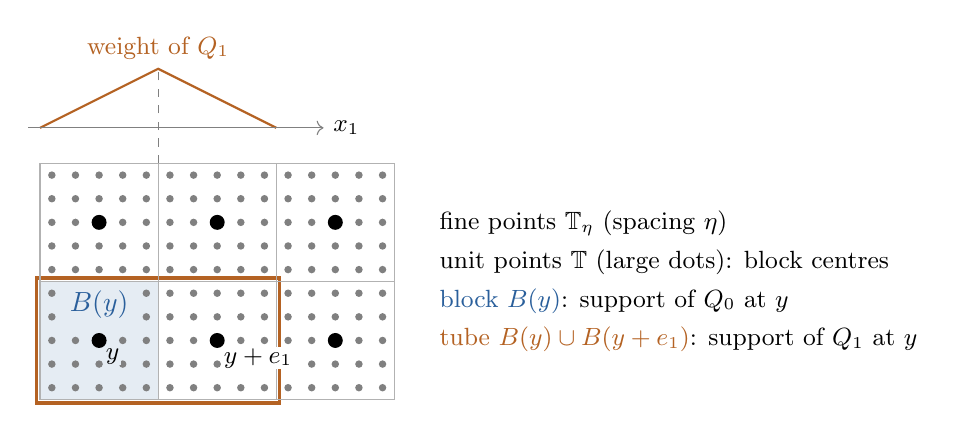
\begin{tikzpicture}[scale=1.5]
% blocks: centred at the unit points, boundaries at half-integers
\fill[fblue!12] (-0.5,-0.5) rectangle (0.5,0.5);
\draw[forange,very thick] (-0.53,-0.53) rectangle (1.53,0.53);
\foreach \x in {-0.5,0.5,1.5,2.5} \draw[gray!60] (\x,-0.5)--(\x,1.5);
\foreach \y in {-0.5,0.5,1.5} \draw[gray!60] (-0.5,\y)--(2.5,\y);
\foreach \i in {-2,...,12} \foreach \j in {-2,...,7} \fill[gray] (\i*0.2,\j*0.2) circle (0.9pt);
\foreach \i in {0,1,2} \foreach \j in {0,1} \fill[black] (\i,\j) circle (1.8pt);
\node[fill=fblue!12,inner sep=0.5pt,anchor=north west,font=\small] at (0.04,-0.05) {$y$};
\node[fill=white,inner sep=0.5pt,anchor=north west,font=\small] at (1.04,-0.05) {$y+e_1$};
\node[fblue,fill=fblue!12,inner sep=1pt] at (0,0.3) {$B(y)$};
% weight profile of Q_1: triangle peaked at the face between B(y) and B(y+e_1)
\draw[gray,dashed] (0.5,1.5)--(0.5,2.3);
\draw[forange,thick] (-0.5,1.8)--(0.5,2.3)--(1.5,1.8);
\draw[gray,->] (-0.6,1.8)--(1.9,1.8) node[right,black] {\small $x_1$};
\node[forange,above] at (0.5,2.3) {\small weight of $Q_1$};
\node[align=left,right] at (2.8,0.5) {\small fine points $\Tf$ (spacing $\eta$)\\[2pt] \small unit points $\T$ (large dots): block centres\\[2pt] \small {\color{fblue}block $B(y)$}: support of $Q_0$ at $y$\\[2pt] \small {\color{forange}tube $B(y)\cup B(y+e_1)$}: support of $Q_1$ at $y$};
\end{tikzpicture}
\caption{A two-dimensional picture of the two lattices, for $N=5$. The blocks are centred at the unit points. The block average $(Q_0f)(y)$ is the mean of $f$ over $B(y)$. The tube average $(Q_1f)(y)$ is the mean over $x\in B(y)$ of the averages of $f$ along the unit segments from $x$ to $x+e_1$. Its weight is the triangle shown above the tube. It is peaked at the face between $B(y)$ and $B(y+e_1)$.}
\label{fig:lattices}
\end{figure}

\subsection{Fields, derivatives and the Hodge identity}\label{ss:2.2}

A \emph{scalar field} is a function $f:\Tf\to\R$. A \emph{gauge field} (a $1$-form) is a $d$-tuple $A=(A_1,\dots,A_d)$ of scalar fields. Here $A_\mu(x)$ is the value of $A$ on the oriented bond $(x,x+\eta e_\mu)$, and the value on the reversed bond is $-A_\mu(x)$. We write $A(b)$ for the value on an oriented bond $b=(b_-,b_+)$, so that $A(-b)=-A(b)$. A map $r\in\mathfrak S_k$ maps oriented bonds to oriented bonds, $rb=(rb_-,rb_+)$, and it acts on gauge fields by $(rA)(b)=A(r^{-1}b)$. A $2$-form is a collection $F=(F_{\mu\nu})$ with $F_{\nu\mu}=-F_{\mu\nu}$. Here $F_{\mu\nu}(x)$ is the value on the plaquette spanned by $x$, $\eta e_\mu$ and $\eta e_\nu$. The inner products are
\[
\ip fg=\eta^d\sum_{x\in\Tf}f(x)g(x),\qquad
\ip AB=\sum_{\mu}\ip{A_\mu}{B_\mu},\qquad
\ip FE=\sum_{\mu<\nu}\ip{F_{\mu\nu}}{E_{\mu\nu}},
\]
and $\|\cdot\|$ denotes the corresponding norms. For a set $X\subset\Tf$, $\|f\|_X$ is the norm of $\one_Xf$. Unit-lattice fields are defined in the same way on $\T$, with inner product $\sum_{y\in\T}$ and no factor $\eta^d$, and $\mathfrak S_k$ acts on them in the same way. With these normalizations a block has volume $\eta^dN^d=1$, so constant fields have comparable norms on both lattices.

The forward and backward derivatives are
\[
(\partial_\mu f)(x)=\frac{f(x+\eta e_\mu)-f(x)}{\eta},\qquad (\partial_\mu^*f)(x)=\frac{f(x-\eta e_\mu)-f(x)}{\eta}.
\]
Then $\partial_\mu^*$ is the adjoint of $\partial_\mu$. All $\partial_\mu$ and $\partial_\nu^*$ commute with one another and with translations of $\Tf$. The exterior derivative and its adjoint are
\begin{align*}
(df)_\mu&=\partial_\mu f, & d^*A&=\sum_\mu\partial_\mu^*A_\mu,\\
(dA)_{\mu\nu}&=\partial_\mu A_\nu-\partial_\nu A_\mu, & (d^*F)_\nu&=\sum_\mu\partial_\mu^*F_{\mu\nu}.
\end{align*}
One checks directly that $d^*$ is the adjoint of $d$ and that $d(df)=0$. The (non-positive) Laplacian is $\Lap=-\sum_\mu\partial_\mu^*\partial_\mu=-d^*d$ on scalar fields. It acts on gauge fields componentwise. We use the shorthand
\[
\|\partial f\|^2=\sum_\mu\|\partial_\mu f\|^2=\ip f{-\Lap f},\qquad
\|\partial A\|^2=\sum_{\mu,\nu}\|\partial_\nu A_\mu\|^2 .
\]
Gauge fields of the form $d\lambda$ are called \emph{exact}, and those with $d^*A=0$ \emph{co-closed}.

\begin{lemma}[Hodge identities]\label{lem:hodge}
For every gauge field $A$,
\[
(d^*d+dd^*)A=-\Lap A\quad\text{(componentwise)},\qquad
\|dA\|^2+\|d^*A\|^2=\|\partial A\|^2 .
\]
Moreover $-\Lap$ is invertible on scalar fields with mean zero, and every gauge field decomposes orthogonally as $A=d\lambda+A'$ with $d^*A'=0$ and $\lambda=(-\Lap)^{-1}d^*A$. The same statements hold on the unit torus, with $\partial_\mu$ replaced by the unit difference $D_\mu g(y)=g(y+e_\mu)-g(y)$.
\end{lemma}

\begin{proof}
For the first identity,
\[
(d^*dA)_\mu=\sum_\nu\partial^*_\nu(\partial_\nu A_\mu-\partial_\mu A_\nu),\qquad (dd^*A)_\mu=\partial_\mu\sum_\nu\partial^*_\nu A_\nu,
\]
and the mixed terms cancel because $\partial_\mu$ and $\partial^*_\nu$ commute. Taking the inner product with $A$ gives the second identity. Next, $-\Lap$ is symmetric and $\ip f{-\Lap f}=\|\partial f\|^2$. This vanishes only for constant $f$ on the connected torus. Hence $-\Lap$ is invertible on the orthogonal complement of the constants. Since $d^*A$ has mean zero ($\ip1{d^*A}=\ip{d1}A=0$), $\lambda$ is well defined. Then $d^*(A-d\lambda)=d^*A+\Lap\lambda=0$, and $\ip{d\lambda}{A'}=\ip\lambda{d^*A'}=0$. The proof on $\T$ is identical.
\end{proof}

On the unit torus we write $\dl$ for the exterior derivative built from $D_\mu$, and $\dl^*$ for its adjoint, with $(D_\mu^*g)(y)=g(y-e_\mu)-g(y)$.

\subsection{Directional convolutions}\label{ss:2.3}

The flat block and tube averages introduced in this section are obtained by restricting products of one-dimensional averages to the unit lattice, so we introduce a convenient language for those products.

\begin{definition}\label{x:2.3}
Let $\mu\in\{1,\dots,d\}$ and let $\kappa:\eta\Z\to\R$ vanish outside an interval of length at most $6$. The \emph{directional convolution} in direction $\mu$ with kernel $\kappa$ is
\[
(Kf)(x)=\sum_{s\in\eta\Z}\eta\,\kappa(s)\,f(x+se_\mu),
\]
where $x+se_\mu$ is taken modulo the torus. Products of directional convolutions in different directions are called \emph{product convolutions}.
\end{definition}

Directional convolutions commute with each other and with all translations of $\Tf$. The adjoint of $K$ has kernel $s\mapsto\kappa(-s)$. The composition of two convolutions in the same direction has kernel $(\kappa_1\star\kappa_2)(s)=\sum_t\eta\,\kappa_1(t)\kappa_2(s-t)$. Moreover $|\kappa_1\star\kappa_2|\le\|\kappa_1\|_\infty\sum_t\eta|\kappa_2(t)|$, and the support lengths add. The box averages $a_\mu$, $a^*_\mu$, $a^c_\mu$ and the triangle average $c_\mu$ defined below have nonnegative kernels of mass $1$, bounded by $1$. Hence every composition of such averages, possibly composed with one further convolution whose kernel is bounded by $M$, has a kernel bounded by $1$ (respectively $M$). Its support length is the sum of the support lengths.

We use the following operators in direction $\mu$:
\begin{itemize}
\item the forward and backward \emph{box averages} $a_\mu$, $a_\mu^*$, with kernels $\one_{[0,1)}$ and $\one_{(-1,0]}$:
\[
(a_\mu f)(x)=\eta\sum_{j=0}^{N-1}f(x+j\eta e_\mu),\qquad (a_\mu^*f)(x)=\eta\sum_{j=0}^{N-1}f(x-j\eta e_\mu);
\]
\item the \emph{centred box average} $a^c_\mu$, with kernel $\one_{[-(1-\eta)/2,(1-\eta)/2]}$:
\[
(a^c_\mu f)(x)=\eta\sum_{|j|\le(N-1)/2}f(x+j\eta e_\mu).
\]
Its kernel is even, so $a^c_\mu$ is self-adjoint;
\item the unit difference $D_\mu f(x)=f(x+e_\mu)-f(x)$, the shift $(\tau_\mu f)(x)=f(x+(1-\eta)e_\mu)$ and the half shift $(\tau^{1/2}_\mu f)(x)=f(x+\frac{1-\eta}2e_\mu)$. The half shift is a shift of $\Tf$, because $N$ is odd, and $(\tau^{1/2}_\mu)^2=\tau_\mu$;
\item the \emph{triangle average} $c_\mu=a_\mu a_\mu^*$.
\end{itemize}

\begin{lemma}[One-dimensional identities]\label{lem:1d}
For each $\mu$:
\begin{enumerate}[label=(\alph*)]
\item $D_\mu=a_\mu\partial_\mu=\partial_\mu a_\mu$ and $D_\mu^*=a_\mu^*\partial_\mu^*$;
\item $a_\mu=\tau_\mu a_\mu^*$;
\item[(b$'$)] $a^c_\mu=\tau^{1/2}_\mu a^*_\mu$, and hence $a_\mu=\tau^{1/2}_\mu a^c_\mu$;
\item $c_\mu$ has kernel $c(s)=(1-|s|)_+$, and $\sum_s\eta\,c(s)=1$;
\item $1-c_\mu=e_\mu\partial_\mu^*\partial_\mu$, where $e_\mu$ has a kernel $k$ with $0\le k\le\frac12$, $k(s)=0$ for $|s|\ge1$, and $|k(s)-k(s')|\le|s-s'|$. Consequently $e_\mu\partial_\mu$ is a directional convolution with kernel $k_1(s)=(k(s-\eta)-k(s))/\eta$, which satisfies $|k_1|\le1$ and vanishes outside $[-1,1+\eta]$;
\item $a_\mu-1=g_\mu\partial_\mu$, where $g_\mu$ has kernel $(1-\eta-s)\one_{[0,1)}(s)\in[0,1]$.
\end{enumerate}
\end{lemma}

\begin{proof}
All identities are between convolution operators, so it suffices to check them on $\eta\Z$, i.e.\ for functions of one variable $t$. The torus versions follow by periodization.

(a) $(a\partial f)(t)=\eta\sum_{j=0}^{N-1}\frac{f(t+(j+1)\eta)-f(t+j\eta)}{\eta}=f(t+1)-f(t)$, since $N\eta=1$. Taking adjoints gives the second identity.

(b) $(\tau a^*f)(t)=\eta\sum_{j=0}^{N-1}f(t+1-\eta-j\eta)=\eta\sum_{j'=0}^{N-1}f(t+j'\eta)$, with $j'=N-1-j$.

(b$'$) $(\tau^{1/2}a^*f)(t)=\eta\sum_{j=0}^{N-1}f(t+\frac{N-1}2\eta-j\eta)=\eta\sum_{|j'|\le(N-1)/2}f(t+j'\eta)$, with $j'=\frac{N-1}2-j$. The second identity follows from the first and (b), since $\tau^{1/2}a^c=\tau a^*=a$.

(c) The kernel of $aa^*$ at $s\in\eta\Z$ is $\eta\cdot\#\{t\in\eta\Z: t\in[0,1),\ s-t\in(-1,0]\}$. For $0\le s<1$ the admissible $t$ are $s,s+\eta,\dots,1-\eta$, which gives $\eta\cdot(1-s)/\eta=1-s$. The case $s<0$ is symmetric. Finally $\sum_s\eta\,c(s)=\eta\big(1+2\sum_{j=1}^{N-1}(1-j\eta)\big)=\eta(2N-1-(N-1))=1$.

(d) Let $-\Lap_1h(t)=\eta^{-2}(2h(t)-h(t+\eta)-h(t-\eta))$ denote the one-dimensional operator $\partial^*\partial$. A direct check shows $-\Lap_1(-|t|/2)=\eta^{-1}\delta_{t,0}$. Put
\[
k(t)=-\frac{|t|}2+\frac12\sum_s\eta\,|t-s|\,c(s).
\]
Then $-\Lap_1k=\eta^{-1}\delta_{\cdot,0}-c$. Hence the convolution $e$ with kernel $k$ satisfies $e\,\partial^*\partial f=(-\Lap_1k)\star f=f-cf$. If $|t|\ge1$, then $|t-s|=|t|-\operatorname{sgn}(t)s$ for all $s$ in the support of $c$. Since $c$ has mass $1$ and mean $0$, this gives $k(t)=0$. For $|t|<1$, the triangle inequality and $\sum\eta c(s)(t-s)=t$ give $k(t)\ge0$, while $\sum_s\eta|t-s|c(s)\le|t|+1$ gives $k(t)\le\frac12$. Each of the two terms defining $k$ is Lipschitz with constant $\frac12$. The formula for the kernel of $e\partial$ follows by summation by parts: $\sum_s\eta k(s)\frac{f(t+s+\eta)-f(t+s)}\eta=\sum_s\eta\frac{k(s-\eta)-k(s)}\eta f(t+s)$.

(e) $(a f)(t)-f(t)=\eta\sum_{j=0}^{N-1}\sum_{i=0}^{j-1}\eta\,\partial f(t+i\eta)=\sum_{i=0}^{N-1}\eta\,\eta(N-1-i)\,\partial f(t+i\eta)$, and $\eta(N-1-i)=1-\eta-i\eta$.
\end{proof}

\subsection{Averaging operators}\label{ss:2.4}

Let $\iota$ denote restriction to the unit torus, $(\iota f)(y)=f(y)$ for $y\in\T$. Its adjoint is $(\iota^*g)(x)=\eta^{-d}g(x)$ if $x\in\T$ and $0$ otherwise. Put $b=a^c_1a^c_2\cdots a^c_d$, the centred average over the cube of side $1-\eta$ about the point.

\begin{definition}[Averaging operators]\label{def:averages}
The \emph{block average} $Q_0$ and the \emph{tube averages} $Q_\mu$, $\mu=1,\dots,d$, map scalar fields on $\Tf$ to scalar fields on $\T$:
\begin{align*}
(Q_0f)(y)&=(\iota bf)(y)=\eta^d\sum_{x\in B(y)}f(x),\\
(Q_\mu f)(y)&=(\iota a_\mu bf)(y)=\eta^d\sum_{x\in B(y)}\ \eta\sum_{j=0}^{N-1}f(x+j\eta e_\mu).
\end{align*}
The \emph{gauge-field average} maps gauge fields on $\Tf$ to gauge fields on $\T$:
\[
(\bQ A)_\mu=Q_\mu A_\mu,\qquad\text{i.e.}\qquad (\bQ A)_\mu(y)=\eta^d\sum_{x\in B(y)}\eta\sum_{j=0}^{N-1}A_\mu(x+j\eta e_\mu).
\]
We write $Q_\sigma$, $\sigma\in\{0,1,\dots,d\}$, when a statement holds for all of them, and $\cK_\sigma$ for the product convolution with $Q_\sigma=\iota\cK_\sigma$ ($\cK_0=b$, $\cK_\mu=a_\mu b$).
\end{definition}

The gauge-field average is the linearization at $U=1$ of Ba\l aban's averaging. In four dimensions the one-step averaging is \cite[(0.12)]{BalYM4I}, and we construct it in Section~\ref{sec:averaging}. Besides the straight segments from the points $x$ of a block to their translates $x+e_\mu$, it contains contour terms, built from averages over the coordinate-ordered contours inside the blocks. At $U=1$ these terms vanish in the averaged axial gauge of Section~\ref{sec:adapted}. Dropping them is the ``second point of view'' of \cite[(1.13)]{BalPropI}, which we adopt. What remains is $\sum_{x\in B(y)}\eta^{d+1}A([x,x+e_\mu])$, as in \cite[(1.11), (1.18)]{BalPropI}, where $A([x,x+e_\mu])$ is the sum of $A$ over the unit segment from $x$ to $x+e_\mu$. This is exactly $(\bQ A)_\mu(y)$. That the composition of $k$ gauge-adapted one-step averagings (Definition~\ref{def:adapted}) linearizes to $\bQ$ is Proposition~\ref{prop:linearized-averages}(c); the plain composition of the averagings \eqref{eq:one-step} linearizes to $\bQ$ minus coarse gradients (Lemma~\ref{lem:one-step-expansion}(f)).

\begin{lemma}[Properties of the averages]\label{lem:avg}
\begin{enumerate}[label=(\alph*)]
\item $(Q_\sigma f)(y)=\eta^d\sum_xw_\sigma(y,x)f(x)$ with $0\le w_\sigma\le1$, $\eta^d\sum_xw_\sigma(y,x)=1$ and $\sum_yw_\sigma(y,x)=1$. Moreover $w_0(y,x)=\one_{B(y)}(x)$, and $w_\mu(y,\cdot)$ vanishes outside $B(y)\cup B(y+e_\mu)$.
\item $Q_\sigma1=1$ and $Q_\sigma^*1=1$. Further, $(Q_0^*g)(x)=g(y(x))$, $Q_0Q_0^*=I$, and $Q_0^*Q_0$ is the orthogonal projection onto fields that are constant on each block.
\item $|(Q_\sigma f)(y)|^2\le\eta^d\sum_xw_\sigma(y,x)|f(x)|^2$. Hence $\|Q_\sigma\|\le1$, $\|\bQ\|\le1$, and $|(Q_\sigma^* g)(x)|\le\max\{|g(y)|:w_\sigma(y,x)\neq0\}$, where at most two $y$ occur.
\item \emph{(Gauge covariance.)} $D_\mu Q_0=Q_\mu\partial_\mu$, i.e.\ $\bQ\,d=\dl Q_0$. More generally, $D_\mu Q_\sigma=\iota\,a_\mu\cK_\sigma\partial_\mu$.
\item \emph{(Curvature.)} $\dl\bQ=\bQ^{(2)}d$, where $(\bQ^{(2)}F)_{\mu\nu}=\iota\,a_\mu a_\nu b\,F_{\mu\nu}$.
\item \emph{(Lattice symmetry.)} For every $r\in\mathfrak S_k$, $Q_0r=rQ_0$ on scalar fields and $\bQ r=r\bQ$ on gauge fields.
\end{enumerate}
\end{lemma}

\begin{proof}
(a) For $Q_0$ this is the definition. For $Q_\mu$, the coefficient of $f(x)$ in $(Q_\mu f)(y)$ is $\eta^{d}\cdot\eta\,\#\{j\in\{0,\dots,N-1\}:x-j\eta e_\mu\in B(y)\}$. So $w_\mu(y,x)\le\eta N=1$, and $w_\mu(y,x)\neq0$ only if $x\in B(y)\cup B(y+e_\mu)$. The normalization $\eta^d\sum_xw_\sigma=Q_\sigma1=1$ is clear. The identity $\sum_yw_\sigma(y,x)=1$ is $Q_\sigma^*1=1$, which follows from $a_\mu^*1=1$ and $(b\,\iota^*g)(x)=g(y(x))$. Here $b=b^*$, since the kernels of the $a^c_\nu$ are even, and $(b\,\iota^*g)(x)$ is the sum of $g(y)$ over the $y\in\T$ with $x\in B(y)$; there is exactly one such $y$, because the blocks partition $\Tf$.

(b) This follows from (a). Moreover $(Q_0Q_0^*g)(y)=\eta^d\sum_{x\in B(y)}g(y)=g(y)$. Hence $Q_0^*Q_0$ is a self-adjoint idempotent, and its range consists of the block-constant fields.

(c) The first bound is Cauchy--Schwarz with the probability weights $\eta^dw_\sigma(y,\cdot)$. Summing over $y$ and using $\sum_yw_\sigma(y,x)=1$ gives $\|Q_\sigma f\|^2\le\|f\|^2$. (Below we sometimes use the weaker bound $\|Q_\sigma\|^2\le2$.) The bound on $Q_\sigma^*g$ follows from $(Q_\sigma^*g)(x)=\sum_yw_\sigma(y,x)g(y)$ and $\sum_yw_\sigma(y,x)=1$.

(d) $\iota$ commutes with unit translations, so $D_\mu Q_\sigma=\iota D_\mu\cK_\sigma=\iota\cK_\sigma a_\mu\partial_\mu$ by Lemma~\ref{lem:1d}(a). For $\sigma=0$ this equals $\iota a_\mu b\,\partial_\mu=Q_\mu\partial_\mu$.

(e) $(\dl\bQ A)_{\mu\nu}=D_\mu Q_\nu A_\nu-D_\nu Q_\mu A_\mu=\iota\,a_\nu b\,a_\mu\partial_\mu A_\nu-\iota\,a_\mu b\,a_\nu\partial_\nu A_\mu$, by (a) of Lemma~\ref{lem:1d}.

(f) Let $r\in\mathfrak S_k$. Since $r^{-1}B(y)=B(r^{-1}y)$,
\[
(Q_0rf)(y)=\eta^d\sum_{x\in B(y)}f(r^{-1}x)=\eta^d\sum_{x'\in B(r^{-1}y)}f(x')=(rQ_0f)(y).
\]
For $\bQ$ we use oriented unit bonds $c=(c_-,c_+)$, and write $(\bQ A)(c)$ for the value of $\bQ A$ on $c$. For fine points $x,x'$ that differ by a unit vector $\pm e_\mu$, let $A([x,x'])$ be the sum of $A$ over the $N$ bonds of the straight segment from $x$ to $x'$, oriented from $x$ to $x'$. We claim that for every oriented unit bond $c$,
\[
(\bQ A)(c)=\eta^{d+1}\sum_{x\in B(c_-)}A\big([x,x+c_+-c_-]\big).
\]
For $c=(y,y+e_\mu)$ this is Definition~\ref{def:averages}, because $\eta\sum_{j=0}^{N-1}A_\mu(x+j\eta e_\mu)=\eta A([x,x+e_\mu])$. For the reversed bond $-c$, use $B(y+e_\mu)=B(y)+e_\mu$ and $A([x+e_\mu,x])=-A([x,x+e_\mu])$: the right-hand side for $-c$ is $-(\bQ A)(c)=(\bQ A)(-c)$. This proves the claim. Now $r^{-1}$ is affine, so it maps the segment from $x$ to $x+c_+-c_-$, with its orientation, onto the segment from $r^{-1}x$ to $r^{-1}x+(r^{-1}c)_+-(r^{-1}c)_-$. Hence $(rA)([x,x+c_+-c_-])=A([r^{-1}x,r^{-1}x+(r^{-1}c)_+-(r^{-1}c)_-])$. Substituting $x'=r^{-1}x$, which runs over $r^{-1}B(c_-)=B((r^{-1}c)_-)$, the claim gives
\[
(\bQ rA)(c)=\eta^{d+1}\sum_{x'\in B((r^{-1}c)_-)}A\big([x',x'+(r^{-1}c)_+-(r^{-1}c)_-]\big)=(\bQ A)(r^{-1}c)=(r\bQ A)(c).\qedhere
\]
\end{proof}

Part (d) is the reason for the particular form of $\bQ$. A gauge transformation $A\mapsto A+d\lambda$ changes the average by the unit-lattice gradient of the block average of $\lambda$:
\[
\bQ(A+d\lambda)=\bQ A+\dl Q_0\lambda .
\]
In particular, the gauge transformations that preserve all averages are those with $Q_0\lambda$ constant. Modulo constants, these are those with $Q_0\lambda=0$. This is the residual gauge freedom of the variational problem, cf.\ \cite[(1.13), (1.20)]{BalPropI}.

Part (f) holds because the blocks are centred at the unit points. With blocks having the unit point at a corner, $Q_0$ would commute with the translations of $\T$ but not with $B_4$ about the unit points. Geometrically, (f) says that the tube of $c$, the union of the segments from the points of $B(c_-)$ in the direction of $c$, is mapped onto itself by every $r\in\mathfrak S_k$ with $rc=\pm c$, for instance by the reflection that fixes the midpoint of $c$ and reverses $c$.

\subsection{Restriction of product convolutions}\label{ss:2.5}

The averaging operators restrict a smoothed field to the unit lattice. The following estimate is used whenever we need to bound such restrictions in $\ell^2$.

\begin{lemma}[Restriction lemma]\label{lem:restriction}
Let $\cK=K_1\cdots K_d$ be a product convolution, where $K_\mu$ has a kernel bounded by $M_\mu$ and vanishing outside an interval of length $\ell_\mu\le6$. Then for every scalar field $f$,
\[
\|\iota\cK f\|_{\ell^2(\T)}\le\prod_{\mu=1}^dM_\mu(\ell_\mu+1)\ \|f\| .
\]
\end{lemma}

\begin{proof}
Write $(\cK f)(y)=\sum_t\eta^d\kappa(t)f(y+t)$ with $\kappa(t)=\prod_\mu\kappa_\mu(t_\mu)$. By Cauchy--Schwarz,
\[
|(\cK f)(y)|^2\le\Big(\sum_t\eta^d|\kappa(t)|\Big)\Big(\sum_t\eta^d|\kappa(t)|\,|f(y+t)|^2\Big).
\]
The first factor is at most $\prod_\mu M_\mu(\ell_\mu+\eta)$. Summing the second factor over $y\in\T$ gives $\sum_x\eta^d|f(x)|^2\sum_y|\kappa(x-y)|$. For fixed $x$ and $\mu$, at most $\ell_\mu+1$ integers $y_\mu$ satisfy $\kappa_\mu(x_\mu-y_\mu)\neq0$. Since $\ell_\mu+1\le7<n$, no point is counted twice on the torus. Hence $\sum_y|\kappa(x-y)|\le\prod_\mu M_\mu(\ell_\mu+1)$.
\end{proof}

When several convolutions act in the same direction, they are first merged into one directional convolution, using the composition rule above. For example, $Q_\sigma$ itself, $\iota\,a_\mu a_\nu b$, and $\iota\,b\,g_\mu$ satisfy the hypotheses with absolute constants. A shift $\tau_\mu$ or $\tau^{1/2}_\mu$ composed with a convolution only moves the support of the kernel, so it does not change the bound.

\section{Poincar\'e inequalities and scalar coercivity}\label{sec:poincare}

The Laplacian $-\Lap$ on $\Tf$ has eigenvalues as small as $(2\pi/n)^2$. So it controls a field only up to modes that vary on the scale of the whole torus. The averaging term $a\|Q_\sigma f\|^2$ supplies the missing control on the unit scale. The precise statement is a Poincar\'e inequality on unit blocks, uniform in~$\eta$.

\begin{lemma}[Block Poincar\'e inequality]\label{lem:block-poincare}
For every block $B=B(y)$ and every scalar field $f$,
\[
\|f-(Q_0f)(y)\|_B^2\le\frac d2\,\eta^d\sum_{b\subset B}|\partial f(b)|^2 .
\]
Here the sum runs over all fine bonds $b=(x,x+\eta e_\mu)$ with both endpoints in $B$, and $\partial f(b)=\partial_\mu f(x)$. Consequently, for every scalar field $f$,
\begin{equation}\label{eq:poincare}
\|f-Q_0^*Q_0f\|^2\le\frac d2\|\partial f\|^2,\qquad \|f\|^2\le\frac d2\|\partial f\|^2+\|Q_0f\|^2 .
\end{equation}
\end{lemma}

\begin{proof}
Let $\bar f=(Q_0f)(y)$ be the mean of $f$ over $B$. Since $B$ has $N^d$ points and volume $1$,
\[
\|f-\bar f\|_B^2=\eta^d\sum_{x\in B}|f(x)-\bar f|^2=\frac{\eta^{2d}}2\sum_{x,x'\in B}|f(x)-f(x')|^2 .
\]
For $x,x'\in B$ we join $x'$ to $x$ by the lattice path that first moves in direction $1$ from $x'_1$ to $x_1$, then in direction $2$ from $x'_2$ to $x_2$, and so on. It stays in $B$ and has at most $d(N-1)$ steps. Then $f(x)-f(x')$ is a sum of at most $dN$ terms $\pm\eta\,\partial f(b)$, and by Cauchy--Schwarz
\[
|f(x)-f(x')|^2\le dN\eta^2\sum_{b\in\text{path}(x',x)}|\partial f(b)|^2=d\eta\sum_{b\in\text{path}(x',x)}|\partial f(b)|^2 .
\]
A bond $b=(z,z+\eta e_\mu)$ lies on the $\mu$-th segment of the path only if $z_\nu=x_\nu$ for $\nu<\mu$ and $z_\nu=x'_\nu$ for $\nu>\mu$. The remaining free coordinates are $x'_\nu$ for $\nu<\mu$, $x_\nu$ for $\nu>\mu$, and the pair $(x_\mu,x'_\mu)$. Hence at most $N^{\mu-1}\cdot N^{d-\mu}\cdot N^2=N^{d+1}$ pairs $(x,x')$ use $b$. Therefore
\[
\|f-\bar f\|_B^2\le\frac{\eta^{2d}}2\,d\eta\,N^{d+1}\sum_{b\subset B}|\partial f(b)|^2=\frac d2\,\eta^d\sum_{b\subset B}|\partial f(b)|^2,
\]
using $\eta N=1$. Summing over blocks gives the first inequality in \eqref{eq:poincare}, since bonds between different blocks only add to the right-hand side. The second follows from the orthogonal decomposition $f=(f-Q_0^*Q_0f)+Q_0^*Q_0f$ and $\|Q_0^*Q_0f\|=\|Q_0f\|$ (Lemma~\ref{lem:avg}(b)).
\end{proof}

\begin{lemma}[Comparison of averages]\label{lem:compare-avg}
For $\mu=1,\dots,d$ and every scalar field $f$,
\[
\|Q_\mu f-Q_0f\|\le 3\cdot2^d\,\|\partial_\mu f\|,\qquad
\|D_\nu Q_\sigma f\|\le 6^d\,\|\partial_\nu f\|\quad(\sigma=0,\dots,d).
\]
\end{lemma}

\begin{proof}
By Lemma~\ref{lem:1d}(e), $Q_\mu f-Q_0f=\iota\,b(a_\mu-1)f=\iota\,b\,g_\mu\,\partial_\mu f$. In direction $\mu$ the operator $a^c_\mu g_\mu$ has a kernel bounded by $1+\eta\le2$ and supported in an interval of length $2$. In every other direction the kernel is $\one_{[-(1-\eta)/2,(1-\eta)/2]}$. Lemma~\ref{lem:restriction} gives the constant $2\cdot3\cdot2^{d-1}$. Similarly, $D_\nu Q_\sigma f=\iota\,a_\nu\cK_\sigma\partial_\nu f$ by Lemma~\ref{lem:avg}(d). This is a product of at most three box averages in each direction, with kernels bounded by $1$ and supported in intervals of length at most $3$. Lemma~\ref{lem:restriction} gives a factor at most $4$ in direction $\nu$ and at most $3$ in each other direction.
\end{proof}

\begin{corollary}[Poincar\'e inequality for all averages]\label{cor:poincare-all}
There is an absolute constant $C_P$ such that for every $\sigma\in\{0,\dots,d\}$ and every scalar field $f$,
\[
\|f\|^2\le C_P\big(\|\partial f\|^2+\|Q_\sigma f\|^2\big).
\]
For gauge fields, $\|A\|^2\le C_P\big(\|\partial A\|^2+\|\bQ A\|^2\big)$.
\end{corollary}

\begin{proof}
By \eqref{eq:poincare} and Lemma~\ref{lem:compare-avg}, $\|f\|^2\le\frac d2\|\partial f\|^2+2\|Q_\sigma f\|^2+2\cdot9\cdot4^d\|\partial f\|^2$. Apply this to each component $A_\mu$ with $\sigma=\mu$ and sum over $\mu$.
\end{proof}

\begin{corollary}[Scalar coercivity]\label{cor:scalar-coercive}
Let $a>0$ and $c_0=\min(1,a)/(2+2C_P)$. For every $\sigma$ and every scalar field $f$,
\[
\ip f{(-\Lap+aQ_\sigma^*Q_\sigma)f}=\|\partial f\|^2+a\|Q_\sigma f\|^2\ge c_0\big(\|f\|^2+\|\partial f\|^2\big).
\]
In particular $-\Lap+aQ_\sigma^*Q_\sigma$ is invertible, and its inverse $G_\sigma$ satisfies $0<G_\sigma\le c_0^{-1}$.
\end{corollary}

\begin{proof}
$\|\partial f\|^2+a\|Q_\sigma f\|^2\ge\min(1,a)\big(\frac12\|\partial f\|^2+\frac12(\|\partial f\|^2+\|Q_\sigma f\|^2)\big)$. Then use Corollary~\ref{cor:poincare-all} on the last bracket.
\end{proof}

This is the scalar half of Theorem~\ref{thm:A}. The next lemma is used in the gauge-field part. It concerns fields with vanishing block averages, i.e.\ generators of the residual gauge transformations.

\begin{lemma}[Fields with vanishing averages]\label{lem:kerQ0}
If $Q_0\lambda=0$, then
\[
\|\lambda\|\le\sqrt{d/2}\,\|\partial\lambda\|,\qquad \|\partial\lambda\|\le\sqrt{d/2}\,\|\Lap\lambda\| .
\]
In particular $-\Lap$ is injective on $\cN(Q_0)=\{\lambda:Q_0\lambda=0\}$.
\end{lemma}

\begin{proof}
The first inequality is \eqref{eq:poincare} with $Q_0\lambda=0$. For the second, $\|\partial\lambda\|^2=\ip\lambda{-\Lap\lambda}\le\|\lambda\|\|\Lap\lambda\|\le\sqrt{d/2}\,\|\partial\lambda\|\,\|\Lap\lambda\|$.
\end{proof}

\section{Two Fourier estimates}\label{sec:fourier}

Fourier analysis plays only a small role in this paper. Its main use is to show that averaged Green functions such as $Q_\sigma G_\sigma Q_\sigma^*$ are bounded \emph{below} uniformly in $\eta$. Upper bounds and decay are proved in position space. We also need one estimate on ``biharmonic extensions'' in the gauge-field coercivity proof.

\subsection{Fourier transform and Bloch decomposition}\label{ss:4.1}

The dual of the fine torus is $\Tf^*=\big((2\pi/n)\Z\big/(2\pi/\eta)\Z\big)^d$. We represent it by the momenta $p$ with $-\pi/\eta<p_\mu\le\pi/\eta$. For a scalar field $f$ we put
\[
\hat f(p)=\eta^d\sum_{x\in\Tf}e^{-\ii p\cdot x}f(x),\qquad f(x)=n^{-d}\sum_{p\in\Tf^*}e^{\ii p\cdot x}\hat f(p),\qquad \|f\|^2=n^{-d}\sum_p|\hat f(p)|^2 .
\]
On the unit torus, $\hat g(q)=\sum_{y\in\T}e^{-\ii q\cdot y}g(y)$ for $q\in\T^*$, which we represent by $-\pi<q_\mu\le\pi$, and $\|g\|^2=n^{-d}\sum_q|\hat g(q)|^2$.

Every $p\in\Tf^*$ can be written uniquely as $p=q+2\pi l$ with $q\in\T^*$ and $l\in\Z^d$. For fixed $q$ exactly $N^d$ vectors $l$ occur. This is the \emph{Bloch decomposition}.

A directional convolution with kernel $\kappa$ in direction $\mu$ acts in momentum space as multiplication by $\tilde\kappa(p_\mu)$, where $\tilde\kappa(\theta)=\sum_s\eta\,\kappa(s)e^{\ii\theta s}$. Its adjoint has symbol $\overline{\tilde\kappa}$. In particular
\[
\widehat{\partial_\mu f}(p)=\frac{e^{\ii\eta p_\mu}-1}\eta\,\hat f(p),\qquad
\widehat{-\Lap f}(p)=\hat\Lap(p)\hat f(p),\quad \hat\Lap(p)=\sum_\mu\frac4{\eta^2}\sin^2\frac{\eta p_\mu}2,
\]
and $a_\mu$ has symbol $\alpha(p_\mu)$, with
\[
\alpha(\theta)=\eta\sum_{j=0}^{N-1}e^{\ii j\eta\theta}=\eta\,\frac{e^{\ii\theta}-1}{e^{\ii\eta\theta}-1},\qquad |\alpha(\theta)|=\frac{|\sin(\theta/2)|}{N|\sin(\eta\theta/2)|}.
\]
The centred box average $a^c_\mu$ has the real symbol
\[
\alpha_c(\theta)=\eta\sum_{|j|\le(N-1)/2}e^{\ii j\eta\theta}=\frac{\sin(\theta/2)}{N\sin(\eta\theta/2)}=e^{-\ii(1-\eta)\theta/2}\alpha(\theta),
\]
by Lemma~\ref{lem:1d}(b$'$). In particular $|\alpha_c|=|\alpha|$, so every bound below on $|\alpha|$ holds for $|\alpha_c|$.
Restriction to the unit lattice and its adjoint satisfy the \emph{Poisson summation formula}:
\begin{equation}\label{eq:poisson}
\widehat{\iota f}(q)=\sum_{l}\hat f(q+2\pi l),\qquad \widehat{\iota^*g}(p)=\hat g(q)\quad\text{for }p=q+2\pi l .
\end{equation}
The first identity follows by inserting the inversion formula for $f$ into $\sum_ye^{-\ii q\cdot y}f(y)$ and using $\sum_{y\in\T}e^{\ii(p-q)\cdot y}=n^d\one[p-q\in2\pi\Z^d]$. The second is immediate from the definition of $\iota^*$.

\begin{lemma}[Symbol bounds]\label{lem:symbols}
Let $|\theta|\le\pi/\eta$.
\begin{enumerate}[label=(\alph*)]
\item $\frac4{\pi^2}\theta^2\le\frac4{\eta^2}\sin^2\frac{\eta\theta}2\le\theta^2$. Hence $\frac4{\pi^2}|p|^2\le\hat\Lap(p)\le|p|^2$ on the fundamental domain.
\item $|\alpha(\theta)|\le1$, and $|\alpha(\theta)|\ge2/\pi$ if $|\theta|\le\pi$.
\item If $\theta=q+2\pi l$ with $|q|\le\pi$ and $l\in\Z\setminus\{0\}$, then $|\theta|\ge\pi|l|$ and $|\alpha(\theta)|\le|q|/(2|l|)$.
\end{enumerate}
\end{lemma}

\begin{proof}
(a) uses $\frac2\pi t\le\sin t\le t$ for $0\le t\le\pi/2$. (b) The first bound is the triangle inequality. For $|\theta|\le\pi$, $|\sin(\theta/2)|\ge|\theta|/\pi$ and $N|\sin(\eta\theta/2)|\le|\theta|/2$. (c) $|\theta|\ge2\pi|l|-|q|\ge\pi|l|$. Moreover $|\sin(\theta/2)|=|\sin(q/2)|\le|q|/2$, and $N|\sin(\eta\theta/2)|\ge N\frac2\pi\frac{\eta|\theta|}2=|\theta|/\pi\ge|l|$.
\end{proof}

\subsection{The lower bound}\label{ss:4.2}

\begin{lemma}[Fourier lower bound]\label{lem:fourier-lower}
Let $K$ be a translation-invariant operator on scalar fields of $\Tf$ with symbol $\hat K(p)\ge0$ on $\Tf^*$, and let $\cK$ be a product convolution with symbol $\kappa(p)$. Represent each $q\in\T^*$ by $-\pi<q_\mu\le\pi$; this is a point of $\Tf^*$. Then for every field $g$ on $\T$,
\[
\ip{\cK^*\iota^*g}{K\cK^*\iota^*g}\ \ge\ m\,\|g\|^2,\qquad m=\min_{q\in\T^*}\hat K(q)|\kappa(q)|^2 .
\]
\end{lemma}

\begin{proof}
By \eqref{eq:poisson}, $h=\cK^*\iota^*g$ has $\hat h(q+2\pi l)=\overline{\kappa(q+2\pi l)}\,\hat g(q)$. Therefore
\[
\ip h{Kh}=n^{-d}\sum_q|\hat g(q)|^2\sum_l\hat K(q+2\pi l)|\kappa(q+2\pi l)|^2\ \ge\ n^{-d}\sum_q|\hat g(q)|^2\,\hat K(q)|\kappa(q)|^2,
\]
where we kept only the term $l=0$. The claim follows from Parseval on $\T$.
\end{proof}

\begin{corollary}\label{cor:QKQ-lower}
For every $\sigma\in\{0,\dots,d\}$ and $a>0$,
\[
Q_\sigma(-\Lap+2a)^{-1}Q_\sigma^*\ \ge\ c_F,\qquad c_F=\Big(\frac2\pi\Big)^{2d+2}\frac1{d\pi^2+2a}.
\]
\end{corollary}

\begin{proof}
Apply Lemma~\ref{lem:fourier-lower} with $K=(-\Lap+2a)^{-1}$ and $\cK=\cK_\sigma$. The symbol of $\cK_\sigma$ is a product of at most $d+1$ factors $\alpha(p_\nu)$ or $\alpha_c(p_\nu)$, each of modulus at least $2/\pi$ on $[-\pi,\pi]^d$, which contains the representatives of $\T^*$. Moreover $\hat\Lap(p)\le|p|^2\le d\pi^2$ there.
\end{proof}

\subsection{Biharmonic extensions}\label{ss:4.3}

The following estimate is used in Section~\ref{sec:gauge-coercivity}. Given a unit-lattice field $\omega$ with mean zero, the field $\lambda=(-\Lap)^{-2}Q_0^*\omega$ is the smoothest (in the sense of $\|\Lap\lambda\|$) fine field with prescribed block averages $Q_0\lambda$, which then have mean zero. We will see that this is exactly the gradient part of a gauge field in Ba\l aban's gauge. Its energy is controlled by the unit-lattice gradient of its averages.

\begin{lemma}[Biharmonic extensions]\label{lem:biharmonic}
There is an absolute constant $C_B$ with the following property. Let $\omega$ be a field on $\T$ with mean zero, and let $\lambda=(-\Lap)^{-2}Q_0^*\omega$ (the inverse taken on mean-zero fields). Then
\[
\|\partial\lambda\|\le C_B\,\|\dl Q_0\lambda\| .
\]
\end{lemma}

\begin{proof}
Let $\beta(p)=\prod_\nu\alpha_c(p_\nu)$ be the symbol of $b$. By \eqref{eq:poisson}, $\hat\lambda(p)=\overline{\beta(p)}\,\hat\omega(q)\,\hat\Lap(p)^{-2}$ for $p=q+2\pi l\ne0$, and $\hat\lambda(0)=0$. For $j\in\{2,3\}$ and $q\in\T^*\setminus\{0\}$ put $S_j(q)=\sum_l|\beta(q+2\pi l)|^2\hat\Lap(q+2\pi l)^{-j}$. Then
\[
\|\partial\lambda\|^2=\ip\lambda{-\Lap\lambda}=n^{-d}\sum_{q\ne0}|\hat\omega(q)|^2S_3(q).
\]
The term $q=0$ is absent, because $\hat\omega(0)=0$, and because for $l\ne0$ some factor $\alpha_c(2\pi l_\nu)$ vanishes, since $0<|l_\nu|<N$ for some $\nu$ on the fundamental domain. Similarly, $g=Q_0\lambda=\iota b\lambda$ has $\hat g(q)=\sum_l\beta(q+2\pi l)\hat\lambda(q+2\pi l)=\hat\omega(q)S_2(q)$, and
\[
\|\dl g\|^2=n^{-d}\sum_{q\ne0}\hat\Lap_1(q)\,S_2(q)^2\,|\hat\omega(q)|^2,\qquad \hat\Lap_1(q)=\sum_\nu4\sin^2\frac{q_\nu}2 .
\]
It therefore suffices to show $S_3(q)\le C_B^2\hat\Lap_1(q)S_2(q)^2$ for $q\in[-\pi,\pi]^d\setminus\{0\}$.

By Lemma~\ref{lem:symbols}, keeping only the term $l=0$ in $S_2$, we get $S_2(q)\ge(2/\pi)^{2d}|q|^{-4}$, and $\hat\Lap_1(q)\ge\frac4{\pi^2}|q|^2$. Hence
\[
\hat\Lap_1(q)S_2(q)^2\ge\frac4{\pi^2}\Big(\frac2\pi\Big)^{4d}|q|^{-6}.
\]
In $S_3$, the term $l=0$ is at most $(\pi/2)^6|q|^{-6}$. For $l\ne0$, Lemma~\ref{lem:symbols}(a),(c) gives $\hat\Lap(q+2\pi l)\ge\frac4{\pi^2}|q+2\pi l|^2\ge4|l|^2\ge4$ and $|\beta(q+2\pi l)|^2\le\prod_{\nu:\,l_\nu\ne0}\frac{\pi^2}{4l_\nu^2}$. Hence
\[
\sum_{l\ne0}\frac{|\beta(q+2\pi l)|^2}{\hat\Lap(q+2\pi l)^3}\le\frac1{64}\prod_{\nu=1}^d\Big(1+2\sum_{m\ge1}\frac{\pi^2}{4m^2}\Big)=\frac1{64}\Big(1+\frac{\pi^4}{12}\Big)^d .
\]
Since $|q|^2\le d\pi^2$, this constant is at most $\frac1{64}(1+\pi^4/12)^d(d\pi^2)^3|q|^{-6}$, and the lemma follows.
\end{proof}

\section{Operators with exponential decay and the Combes--Thomas method}\label{sec:decay}

Exponential decay will first be established in $L^2$, between unit blocks. This section develops the bookkeeping for this notion and the basic mechanism that produces it: if $K$ is coercive and conjugation by $e^{\alpha\rho}$ changes $K$ only by $O(\alpha)$, then $K^{-1}$ decays exponentially.

\subsection{Block decay}\label{ss:5.1}

We work with four kinds of field spaces: scalar fields and gauge fields on $\Tf$, and scalar fields and gauge fields on $\T$. On each of them we have the \emph{localization projections} $\one_y$, $y\in\T$. On the fine lattice, $\one_y$ is multiplication by the indicator of $B(y)$ (for gauge fields: of the bonds $(x,x+\eta e_\mu)$ with $x\in B(y)$). On the unit lattice, $\one_y$ keeps the value(s) at $y$. In all cases $\sum_y\one_y=I$.

\begin{definition}\label{def:decay}
A linear operator $K$ between two such spaces has \emph{decay $(C,\gamma)$} if
\[
\|\one_yK\one_{y'}\|\le Ce^{-\gamma|y-y'|}\qquad\text{for all }y,y'\in\T .
\]
\end{definition}

For operators between unit-lattice spaces, $\|\one_yK\one_{y'}\|$ is the absolute value (or matrix norm) of the kernel $K(y,y')$, so decay is a pointwise kernel bound. We put
\[
S_\gamma=\sum_{z\in\Z^d}e^{-\gamma|z|}.
\]
Then $\sum_{y'\in\T}e^{-\gamma|y-y'|}\le S_\gamma$ for every $y$, uniformly in $n$, because distinct $y'$ have distinct nearest representatives of $y'-y$ in $\Z^d$.

\begin{lemma}[Calculus of decay]\label{lem:decay-calculus}
\begin{enumerate}[label=(\alph*)]
\item If $K$ has decay $(C,\gamma)$, then $\|K\|\le CS_\gamma$.
\item If $K_1$ and $K_2$ have decay $(C_1,\gamma)$ and $(C_2,\gamma)$, then $K_1K_2$ has decay $(C_1C_2S_{\gamma/2},\gamma/2)$.
\item If $K$ has decay $(C,\gamma)$ then $K^*$ has decay $(C,\gamma)$. Sums behave in the obvious way, and decay $(C,\gamma)$ implies decay $(C,\gamma')$ for $\gamma'\le\gamma$.
\item If $\one_yK\one_{y'}=0$ for $|y-y'|>r$ and $\|K\|\le M$, then $K$ has decay $(Me^{\gamma r},\gamma)$ for every $\gamma>0$.
\end{enumerate}
\end{lemma}

\begin{proof}
(a) $\|\one_yKf\|\le\sum_{y'}Ce^{-\gamma|y-y'|}\|\one_{y'}f\|$. The matrix $(e^{-\gamma|y-y'|})$ has row and column sums at most $S_\gamma$, so by the Schur test it defines an operator on $\ell^2(\T)$ of norm at most $S_\gamma$. Hence $\|Kf\|^2=\sum_y\|\one_yKf\|^2\le C^2S_\gamma^2\sum_{y'}\|\one_{y'}f\|^2$.

(b) $\one_yK_1K_2\one_{y'}=\sum_{y''}\one_yK_1\one_{y''}K_2\one_{y'}$. By the triangle inequality $|y-y''|+|y''-y'|\ge\frac12|y-y'|+\frac12|y-y''|$, so the norm is at most $C_1C_2e^{-\gamma|y-y'|/2}\sum_{y''}e^{-\gamma|y-y''|/2}$.

(c) and (d) are immediate.
\end{proof}

\subsection{Conjugation by exponential weights}\label{ss:5.2}

A function $\rho:\Tf\to\R$ is \emph{$1$-Lipschitz} if $|\rho(x)-\rho(x')|\le|x-x'|$ for all $x,x'$. A typical example is $\rho(x)=\operatorname{dist}(x,B(y'))$, the torus distance to a block. For $\alpha\in\R$, multiplication by $e^{\alpha\rho}$ acts on all four field spaces. On unit-lattice fields it multiplies the value at $y$ by $e^{\alpha\rho(y)}$, which is consistent because $\T\subset\Tf$. For an operator $K$ we write
\[
K_\alpha=e^{\alpha\rho}Ke^{-\alpha\rho}.
\]
Then $(K_1K_2)_\alpha=(K_1)_\alpha(K_2)_\alpha$, $(K^*)_\alpha=(K_{-\alpha})^*$, and $(K^{-1})_\alpha=(K_\alpha)^{-1}$. Since $\iota$ commutes with multiplication operators, $(\iota)_\alpha=\iota$.

\begin{lemma}[Conjugation of decaying operators]\label{lem:conjugation}
Let $K$ have decay $(C,\gamma)$ and let $\rho$ be $1$-Lipschitz. For $|\alpha|\le\gamma/2$,
\[
\|K_\alpha-K\|\le C\,c_1(\gamma)\,|\alpha|,\qquad c_1(\gamma)=e^{\gamma\sqrt d}\big(2\sqrt d+4/\gamma\big)S_{\gamma/4}.
\]
\end{lemma}

\begin{proof}
Fix $y,y'$, put $X=\one_yK\one_{y'}$, and write $e^{\alpha\rho}=e^{\alpha\rho(y)}E$ on the support of $\one_y$. Here $E$ is multiplication by $e^{\alpha(\rho-\rho(y))}$. Since points of $B(y)$ are within distance $\sqrt d$ of $y$, $\|E-1\|\le|\alpha|\sqrt d\,e^{|\alpha|\sqrt d}$ and $\|E\|\le e^{|\alpha|\sqrt d}$. Define $E'$ similarly at $y'$. Then $\one_y(K_\alpha-K)\one_{y'}=sEXE'^{-1}-X$ with $s=e^{\alpha(\rho(y)-\rho(y'))}$. Since $|s-1|\le|\alpha||y-y'|e^{|\alpha||y-y'|}$, the decomposition
\[
sEXE'^{-1}-X=(s-1)EXE'^{-1}+(E-1)XE'^{-1}+X(E'^{-1}-1)
\]
gives
\[
\|\one_y(K_\alpha-K)\one_{y'}\|\le C|\alpha|\,e^{2|\alpha|\sqrt d}\big(|y-y'|+2\sqrt d\big)e^{-(\gamma-|\alpha|)|y-y'|}.
\]
For $|\alpha|\le\gamma/2$ we have $e^{2|\alpha|\sqrt d}\le e^{\gamma\sqrt d}$ and $(t+2\sqrt d)e^{-\gamma t/2}\le(2\sqrt d+4/\gamma)e^{-\gamma t/4}$. Hence $K_\alpha-K$ has decay $(C|\alpha|e^{\gamma\sqrt d}(2\sqrt d+4/\gamma),\gamma/4)$, and Lemma~\ref{lem:decay-calculus}(a) concludes.
\end{proof}

\begin{lemma}[Conjugated derivatives]\label{lem:conj-derivative}
Let $\rho$ be $1$-Lipschitz and $|\alpha|\le1$. Then $(\partial_\mu)_\alpha=\partial_\mu+Y$ and $(\partial_\mu^*)_\alpha=\partial_\mu^*+Y'$, where $Y,Y'$ are operators of norm at most $e|\alpha|$. On gauge fields the same holds componentwise.
\end{lemma}

\begin{proof}
$(e^{\alpha\rho}\partial_\mu e^{-\alpha\rho}u)(x)=\partial_\mu u(x)+\eta^{-1}\big(e^{\alpha(\rho(x)-\rho(x+\eta e_\mu))}-1\big)u(x+\eta e_\mu)$. Moreover $|e^t-1|\le|t|e^{|t|}$ with $|t|\le|\alpha|\eta$. The computation for $\partial_\mu^*$ is the same.
\end{proof}

\subsection{The Combes--Thomas method}\label{ss:5.3}

We give two versions. The first is for bounded operators, typically on the unit lattice. The second is for fine-lattice operators containing $-\Lap$, whose norm is of order $\eta^{-2}$.

\begin{lemma}[Combes--Thomas, bounded version]\label{lem:CT-bounded}
Let $K$ act on one of the four field spaces, have decay $(C,\gamma)$, and satisfy $\ip f{Kf}\ge c\|f\|^2$ for all (real) fields $f$. Put $\gamma'=\min\{\gamma/2,\ c/(2Cc_1(\gamma))\}$. Then $K$ is invertible and $K^{-1}$ has decay $(2c^{-1}e^{2\gamma'\sqrt d},\gamma')$.
\end{lemma}

\begin{proof}
Fix $y'$, let $\rho(x)=\operatorname{dist}(x,B(y'))$ and $\alpha=\gamma'$. By Lemma~\ref{lem:conjugation}, $\ip f{K_\alpha f}\ge c\|f\|^2-\frac c2\|f\|^2$. Hence $K_\alpha$ is invertible with $\|K_\alpha^{-1}\|\le2/c$. Here we use that in finite dimensions $\ip f{Xf}\ge\delta\|f\|^2$ implies $\|Xf\|\ge\delta\|f\|$. Now $K^{-1}=e^{-\alpha\rho}K_\alpha^{-1}e^{\alpha\rho}$. On the support of $\one_{y'}$ we have $\rho=0$. On the support of $\one_y$ we have $\rho\ge|y-y'|-2\sqrt d$. Therefore $\|\one_yK^{-1}\one_{y'}\|\le e^{-\alpha(|y-y'|-2\sqrt d)}\,2/c$.
\end{proof}

\begin{lemma}[Neumann series]\label{lem:neumann}
Let $\mathfrak N$ have decay $(C,\gamma)$ and $\|\mathfrak N\|\le\theta<1$. Then $(I+\mathfrak N)^{-1}$ has decay $(2(1-\theta)^{-1}e^{2\gamma'\sqrt d},\gamma')$ with $\gamma'=\min\{\gamma/2,(1-\theta)/(2Cc_1(\gamma))\}$.
\end{lemma}

\begin{proof}
As above, with $\|\mathfrak N_\alpha\|\le\theta+(1-\theta)/2$, so that $\|(I+\mathfrak N_\alpha)^{-1}\|\le2/(1-\theta)$.
\end{proof}

This lemma is the form in which exponential decay is used in the variational problem, cf.\ \cite[(68)--(71)]{BalVar}.

For the fine-lattice operators we write $\partial$ for the collection $(\partial_\mu)_\mu$ acting on scalar fields, or componentwise on gauge fields, and $\partial^*$ for its adjoint.

\begin{lemma}[Combes--Thomas, form version]\label{lem:CT-form}
Let $\mathfrak A$ act on scalar or gauge fields on $\Tf$. Suppose that:
\begin{enumerate}[label=(\roman*)]
\item $\ip u{\mathfrak Au}\ge c\,(\|u\|^2+\|\partial u\|^2)$ for all $u$;
\item there are $C_1,\alpha_1>0$ such that for every $1$-Lipschitz $\rho$, every $|\alpha|\le\alpha_1$ and every $u$,
\[
|\ip u{(\mathfrak A_\alpha-\mathfrak A)u}|\le C_1|\alpha|\,(\|u\|^2+\|\partial u\|^2).
\]
\end{enumerate}
Let $\gamma_0=\min\{\alpha_1,1/3,c/(2C_1)\}$. Then the four operators $\mathfrak A^{-1}$, $\partial\mathfrak A^{-1}$, $\mathfrak A^{-1}\partial^*$ and $\partial\mathfrak A^{-1}\partial^*$ have decay $(C_0,\gamma_0)$, with $C_0=2(1+\sqrt d)^2c^{-1}e^{2\gamma_0\sqrt d}$.
\end{lemma}

\begin{proof}
Let $|\alpha|\le\gamma_0$. By (i) and (ii), $\ip u{\mathfrak A_\alpha u}\ge\frac c2(\|u\|^2+\|\partial u\|^2)$, so $\mathfrak A_\alpha$ is invertible. Let $u=\mathfrak A_\alpha^{-1}h$. Then $\frac c2(\|u\|^2+\|\partial u\|^2)\le\|u\|\|h\|$. This gives $\|u\|\le\frac2c\|h\|$ and then $\|\partial u\|^2\le\frac2c\|u\|\|h\|\le\frac4{c^2}\|h\|^2$. If instead $h=\partial^*g$, then $\frac c2(\|u\|^2+\|\partial u\|^2)\le\ip{\partial u}g\le\|\partial u\|\|g\|$, which gives $\|\partial u\|\le\frac2c\|g\|$ and $\|u\|\le\frac2c\|g\|$. Thus
\[
\|\mathfrak A_\alpha^{-1}\|,\ \|\partial\mathfrak A_\alpha^{-1}\|,\ \|\mathfrak A_\alpha^{-1}\partial^*\|,\ \|\partial\mathfrak A_\alpha^{-1}\partial^*\|\le\frac2c .
\]
Now fix $y'$, let $\rho=\operatorname{dist}(\cdot,B(y'))$ and $\alpha=\gamma_0$. By Lemma~\ref{lem:conj-derivative}, $\partial e^{-\alpha\rho}=e^{-\alpha\rho}(\partial+Y)$ and $e^{\alpha\rho}\partial^*=(\partial^*+Y'^{*})e^{\alpha\rho}$, where $Y'$ comes from $(\partial)_{-\alpha}$. Here $Y=(Y_\mu)_\mu$ and $Y'$ consist of $d$ operators, each of norm at most $e\alpha$ by Lemma~\ref{lem:conj-derivative}, so $\|Y\|,\|Y'\|\le\sqrt d\,e\alpha$. Hence, for instance,
\[
\one_y\partial\mathfrak A^{-1}\partial^*\one_{y'}=\one_ye^{-\alpha\rho}(\partial+Y)\mathfrak A_\alpha^{-1}(\partial^*+Y'^*)\one_{y'},
\]
where we used $e^{\alpha\rho}\one_{y'}=\one_{y'}$. The middle operator has norm at most $\frac2c(1+\sqrt d\,e\alpha)^2\le\frac2c(1+\sqrt d)^2$, because $e\alpha\le1$, and $\|\one_ye^{-\alpha\rho}\|\le e^{-\alpha(|y-y'|-2\sqrt d)}$. The other three operators are treated in the same way.
\end{proof}

The hypothesis (ii) is verified with the help of the following observation.

\begin{lemma}[Conjugation of quadratic forms]\label{lem:conj-forms}
Let $X=X_0-Z$, where $X_0=\sum_jc_j\,\partial^{(*)}_{\mu_j}$ is a finite linear combination of the operators $\partial_\mu$, $\partial^*_\mu$ (acting componentwise on scalar or gauge fields, with values in the appropriate form degree) with scalar coefficients $\sum_j|c_j|\le M$, and $Z$ is bounded with $\|Z\|\le M$ and $\|Z_\alpha-Z\|\le M|\alpha|$ for $|\alpha|\le\alpha_1\le1$. Then for $|\alpha|\le\alpha_1$,
\[
|\ip u{((X^*X)_\alpha-X^*X)u}|\le C_M|\alpha|\,(\|u\|^2+\|\partial u\|^2),
\]
with $C_M$ depending only on $M$ and $d$.
\end{lemma}

\begin{proof}
By Lemma~\ref{lem:conj-derivative}, applied to each term of $X_0$, $X_\alpha=X+W_\alpha$ with $\|W_\alpha\|\le(eM+M)|\alpha|$. Also $\|X_0u\|\le M\|\partial u\|$. Since $(X^*X)_\alpha=(X_{-\alpha})^*X_\alpha$,
\[
\ip u{((X^*X)_\alpha-X^*X)u}=\ip{W_{-\alpha}u}{Xu}+\ip{Xu}{W_\alpha u}+\ip{W_{-\alpha}u}{W_\alpha u}.
\]
Finally, $\|Xu\|\le M(\|\partial u\|+\|u\|)$.
\end{proof}

\section{Local regularity on the fine lattice}\label{sec:regularity}

The Combes--Thomas method gives $L^2$ bounds between unit blocks. To obtain bounds on values, derivatives and H\"older quotients that are uniform in $\eta$, we use an interior regularity estimate for the lattice Laplacian. This is the lattice analogue of the classical fact that a solution of $-\Lap u=F$ with bounded $F$ is $C^{1,\alpha}$ in the interior for every $\alpha<1$.

\subsection{The Green function of the fine lattice}\label{ss:6.1}

Let $g_1$ be the Green function of $-\Lap$ on the infinite unit lattice $\Z^d$:
\[
g_1(x)=\frac1{(2\pi)^d}\int_{[-\pi,\pi]^d}\frac{e^{\ii p\cdot x}}{\sum_\mu4\sin^2(p_\mu/2)}\,dp ,
\]
which is well defined, since $|p|^{-2}$ is integrable near $0$ in four dimensions, and satisfies $-\Lap g_1=\delta_0$. On $\eta\Z^d$ put $g_\eta(x)=\eta^{2-d}g_1(x/\eta)$. Then the convolution
\[
(\cG h)(x)=\sum_{x'\in\eta\Z^d}\eta^d\,g_\eta(x-x')\,h(x')
\]
satisfies $-\Lap\cG h=h$ and $\cG(-\Lap h)=h$ for every finitely supported $h$ on $\eta\Z^d$. For the second identity, sum by parts. Since $\cG$ is a convolution, it commutes with all lattice derivatives: $\partial_\mu\cG h=(\partial_\mu g_\eta)\star h$, and similarly for $\partial^*_\mu$.

\begin{proposition}[Decay of derivatives]\label{prop:green-eta}
For every word $\partial^\beta$ of length $|\beta|\le3$ in the operators $\partial_\mu,\partial^*_\mu$,
\[
|\partial^\beta g_\eta(x)|\le C_\beta\,(|x|+\eta)^{2-d-|\beta|},\qquad x\in\eta\Z^d,
\]
with $C_\beta$ depending only on $\beta$.
\end{proposition}

\begin{proof}
By scaling, $\partial^\beta g_\eta(x)=\eta^{2-d-|\beta|}(\nabla^\beta g_1)(x/\eta)$, where $\nabla^\beta$ is the corresponding word of unit-lattice differences. By Theorem~\ref{thm:green-unit} in Appendix~\ref{app:green}, $|\nabla^\beta g_1(z)|\le C_\beta(1+|z|)^{2-d-|\beta|}$.
\end{proof}

We also need two elementary lattice sums.

\begin{lemma}[Lattice sums]\label{lem:lattice-sums}
Let $x\in\eta\Z^d$ and $R\ge\eta$.
\begin{enumerate}[label=(\alph*)]
\item For $0\le s<d$: $\sum_{|x'-x|\le R}\eta^d(|x-x'|+\eta)^{-s}\le C_{d,s}R^{d-s}$.
\item For $\sqrt d\,\eta\le r\le R$: $\sum_{r<|x'-x|\le R}\eta^d|x-x'|^{-d}\le C_d\,(1+\log(R/r))$.
\item For $s>d$ and $r\ge\sqrt d\,\eta$: $\sum_{|x'-x|>r}\eta^d|x-x'|^{-s}\le C_{d,s}\,r^{d-s}$.
\end{enumerate}
\end{lemma}

\begin{proof}
Let $W(x')=x'+[-\eta/2,\eta/2)^d$. For $z\in W(x')$ we have $|z-x|+\eta\le(1+\sqrt d)(|x-x'|+\eta)$. Hence each term in (a) is at most $(1+\sqrt d)^s\int_{W(x')}(|z-x|+\eta)^{-s}dz$. The cubes $W(x')$ are disjoint and contained in the ball of radius $R+\sqrt d\eta\le(1+\sqrt d)R$, which gives (a). In (b), $|x-x'|>r\ge\sqrt d\eta$ implies $\frac12|x-x'|\le|z-x|\le\frac32|x-x'|$ for $z\in W(x')$. Hence the sum is at most $(3/2)^d\int_{r/2\le|z-x|\le3R/2}|z-x|^{-d}dz=(3/2)^d|S^{d-1}|\log(3R/r)$. The same comparison gives (c).
\end{proof}

\subsection{The regularity estimate}\label{ss:6.2}

For $z\in\R^d$ and $r>0$ let $\Lam_r=\{x\in\Tf:|x-z|_\infty\le r\}$. Since $n\ge8$, $\Lam_3$ can be identified with a subset of $\eta\Z^d$.

\begin{theorem}[Interior regularity]\label{thm:local-regularity}
Let $\alpha\in(0,1)$. There is $C$, depending only on $\alpha$, such that the following holds for every lattice spacing $\eta\le1$, in particular $\eta=1/N$ with $N\ge1$, and all $z$; for a spacing not of the form $1/N$, $\Lam_r$ is the set of $x\in\eta\Z^d$ with $|x-z|_\infty\le r$. Let $u,F:\Lam_3\to\R$ and $g=(g_\mu):\Lam_3\to\R^d$ satisfy
\[
-\Lap u=F+\sum_\mu\partial^*_\mu g_\mu\qquad\text{at every point of }\Lam_2 .
\]
\begin{enumerate}[label=(\alph*)]
\item If $g=0$: $\ |u|_{\Lam_1}+|\partial u|_{\Lam_1}+\Hol{\partial u}{\Lam_1}\le C\big(|F|_{\Lam_2}+\|u\|_{\Lam_2}\big)$.
\item In general: $\ |u|_{\Lam_1}+\Hol{u}{\Lam_1}\le C\big(|F|_{\Lam_2}+|g|_{\Lam_3}+\|u\|_{\Lam_2}\big)$.
\item If $g=0$: $\ \max_{\mu,\nu}|\partial_\mu\partial_\nu u|_{\Lam_1}\le C\big(|F|_{\Lam_2}+\Hol{F}{\Lam_2}+\|u\|_{\Lam_2}\big)$.
\item (Divergence form with H\"older data.) $\ |u|_{\Lam_1}+|\partial u|_{\Lam_1}+\Hol{\partial u}{\Lam_1}\le C\big(|F|_{\Lam_2}+|g|_{\Lam_3}+\Hol g{\Lam_3}+\|u\|_{\Lam_2}\big)$.
\end{enumerate}
\end{theorem}

\begin{figure}[t]
\centering
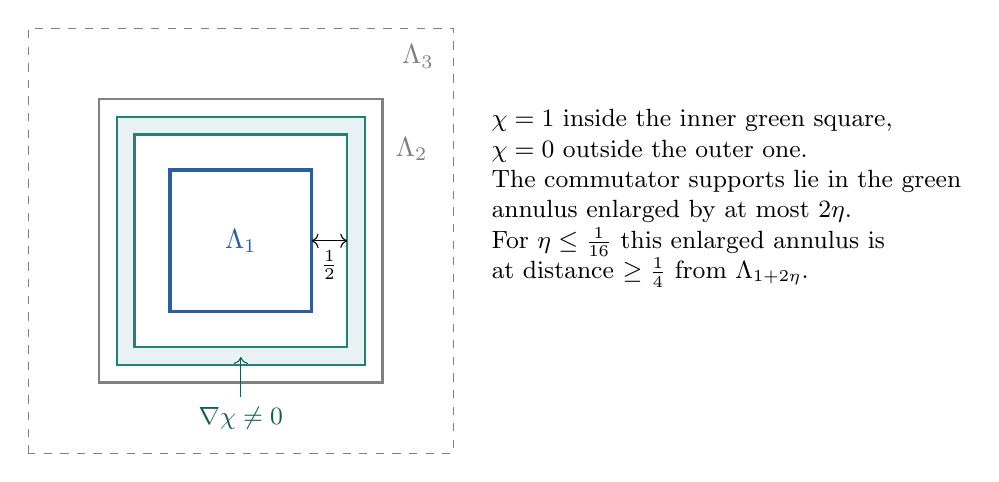
\begin{tikzpicture}[scale=0.9]
\fill[fgreen!10] (-1.75,-1.75) rectangle (1.75,1.75);
\fill[white] (-1.5,-1.5) rectangle (1.5,1.5);
\draw[fblue,very thick] (-1,-1) rectangle (1,1);
\draw[gray,thick] (-2,-2) rectangle (2,2);
\draw[gray,dashed] (-3,-3) rectangle (3,3);
\draw[fgreen,thick] (-1.5,-1.5) rectangle (1.5,1.5);
\draw[fgreen,thick] (-1.75,-1.75) rectangle (1.75,1.75);
\node[fblue] at (0,0) {$\Lam_1$};
\node[gray] at (2.5,2.6) {$\Lam_3$};
\node[gray,anchor=west] at (2.05,1.3) {$\Lam_2$};
\node[fgreen!70!black,font=\small] (lab) at (0,-2.5) {$\nabla\chi\ne0$};\draw[fgreen!70!black,->] (lab.north)--(0,-1.64);
\draw[<->] (1,0)--(1.5,0) node[midway,below,font=\small] {$\tfrac12$};
\node[align=left,anchor=west,font=\small] at (3.4,0.6) {$\chi=1$ inside the inner green square,\\ $\chi=0$ outside the outer one.\\ The commutator supports lie in the green\\ annulus enlarged by at most $2\eta$.\\ For $\eta\le\frac1{16}$ this enlarged annulus is\\ at distance $\ge\frac14$ from $\Lam_{1+2\eta}$.};
\end{tikzpicture}
\caption{Geometry of the proof of Theorem~\ref{thm:local-regularity}.}
\label{fig:cutoff}
\end{figure}

\begin{proof}
\emph{Step 0: coarse lattices.} Let $\eta>\frac1{16}$ (for $\eta=1/N$: $N<16$). Then $|u(x)|\le\eta^{-d/2}\|u\|_{\Lam_2}\le16^{d/2}\|u\|_{\Lam_2}$ for $x\in\Lam_2$, and $\Hol{v}{X}\le2\eta^{-\alpha}|v|_X$. A first difference at a point of $\Lam_1$ involves only points of $\Lam_{1+\eta}\subset\Lam_2$ and costs a factor at most $2/\eta\le32$. This proves (a), (b) and (d). For (c) with $\eta\le\frac12$, a second difference at a point of $\Lam_1$ involves only points of $\Lam_{1+2\eta}\subset\Lam_2$ and costs a factor at most $4/\eta^2$. If $\eta>\frac12$ (for $\eta=1/N$: $N=1$), the difference $\partial_\mu\partial_\mu u(x)$ involves $u(x+2\eta e_\mu)$, which may lie outside $\Lam_2$. Put $v=x+\eta e_\mu$. Since $g=0$ in (c), the equation at $v\in\Lam_2$ gives
\[
\eta^2\partial_\mu\partial_\mu u(x)=(2d-2)\,u(v)-\sum_{\nu\ne\mu}\big(u(v+\eta e_\nu)+u(v-\eta e_\nu)\big)-\eta^2F(v),
\]
and all points on the right lie in $\Lam_2$. The mixed differences $\partial_\mu\partial_\nu u(x)$, $\mu\ne\nu$, involve only points of $\Lam_2$. We assume $\eta\le\frac1{16}$ from now on.

\emph{Step 1: cutoff.} Fix $\chi\in C^\infty(\R^d)$ with $0\le\chi\le1$, $\chi=1$ on $\{|x-z|_\infty\le\frac32\}$ and $\chi=0$ on $\{|x-z|_\infty\ge\frac74\}$. Its lattice differences up to order three are bounded by absolute constants. Let $v=\chi u$, extended by zero to $\eta\Z^d$. Write $S_\mu u(x)=u(x+\eta e_\mu)$. The discrete Leibniz rules
\[
\partial_\mu(\chi u)=\chi\,\partial_\mu u+(\partial_\mu\chi)S_\mu u,\qquad
\partial_\mu^*(\varphi w)=\varphi\,\partial^*_\mu w+(\partial^*_\mu\varphi)S_\mu^{-1}w,
\]
and $S_\mu^{-1}\partial_\mu u=-\partial^*_\mu u$ give, after a short computation,
\begin{equation}\label{eq:commutator}
-\Lap(\chi u)=\chi(-\Lap u)+\sum_\mu\big(\partial^*_\mu m_\mu+n_\mu\big),\qquad
\begin{aligned}
m_\mu&=(\partial_\mu\chi)S_\mu u-(\partial^*_\mu\chi)u,\\
n_\mu&=(\partial^*_\mu\partial^*_\mu\chi)S_\mu^{-1}u .
\end{aligned}
\end{equation}
The functions $m_\mu$, $n_\mu$ vanish outside the annulus $A=\Lam_{7/4+2\eta}\setminus\Lam_{3/2-2\eta}$, where the differences of $\chi$ (up to second order, involving points at distance up to $2\eta$) can be non-zero. They involve $u$ only at points of $\Lam_2$, and $|m_\mu|+|n_\mu|\le C|u|$ at neighbouring points. Similarly $\chi\,\partial^*_\mu g_\mu=\partial^*_\mu(\chi g_\mu)-(\partial^*_\mu\chi)S_\mu^{-1}g_\mu$. Hence
\[
-\Lap v=\Phi_1+\Phi_2+\sum_\mu\partial^*_\mu(\chi g_\mu+m_\mu),\qquad
\Phi_1=\chi F-\sum_\mu(\partial^*_\mu\chi)S^{-1}_\mu g_\mu,\quad \Phi_2=\sum_\mu n_\mu .
\]
All terms vanish outside $\Lam_2$. Since $v$ has finite support,
\begin{equation}\label{eq:rep}
v=\cG\Phi_1+\cG\Phi_2+\sum_\mu(\partial^*_\mu g_\eta)\star(\chi g_\mu)+\sum_\mu(\partial^*_\mu g_\eta)\star m_\mu .
\end{equation}
For $x\in\Lam_{1+2\eta}$ we have $v(x)=u(x)$. So $u$, $\partial u$ and $\partial\partial u$ on $\Lam_1$ can be computed from \eqref{eq:rep}.

\emph{Step 2: the terms supported in the annulus.} Points of $\Lam_{1+2\eta}$ have distance at least $\frac12-4\eta\ge\frac14$ from $A$. By Proposition~\ref{prop:green-eta}, every derivative of order at most three of $g_\eta$ is bounded by a constant on $\{|x|\ge\frac14\}$. Therefore, for $x\in\Lam_{1+2\eta}$ and $|\beta|\le2$,
\[
|\partial^\beta\cG\Phi_2(x)|+\sum_\mu|\partial^\beta(\partial^*_\mu g_\eta)\star m_\mu(x)|\le C\sum_{x'\in A}\eta^d\Big(|\Phi_2(x')|+\sum_\mu|m_\mu(x')|\Big)\le C\|u\|_{\Lam_2},
\]
by Cauchy--Schwarz. For $|\beta|\le1$ the derivatives of order one more are also bounded (they involve at most three derivatives of $g_\eta$), so these terms and their first derivatives are Lipschitz on $\Lam_1$; for (c) only the sup bounds with $|\beta|=2$ are needed. A Lipschitz function on $\Lam_1$ is H\"older: join $x,x'$ by a monotone lattice path inside $\Lam_1$, of length at most $\sqrt d|x-x'|\le2d$.

\emph{Step 3: the near terms in (a) and (b).} Here $\Phi_1$ and $\chi g$ are bounded by $C(|F|_{\Lam_2}+|g|_{\Lam_3})$ and supported in $\Lam_2$. By Lemma~\ref{lem:lattice-sums}(a) with $s=d-2$ and $s=d-1$, for $x\in\Lam_{1+2\eta}$,
\[
|\cG\Phi_1(x)|+|\partial\cG\Phi_1(x)|+|(\partial^*g_\eta)\star(\chi g)(x)|\le C(|F|_{\Lam_2}+|g|_{\Lam_3}).
\]
This proves the sup bounds in (a) and (b), and shows that $\cG\Phi_1$ is Lipschitz on $\Lam_1$. It remains to estimate the H\"older quotient of a convolution $k\star h$ with $|h|\le M$ supported in $\Lam_2$. Here $k=\partial_\mu g_\eta$ in (a), and $k=\partial^*_\mu g_\eta$ in (b). In both cases $|k(y)|\le C(|y|+\eta)^{1-d}$, and every first difference of $k$ is bounded by $C(|y|+\eta)^{-d}$. Let $x,x'\in\Lam_1$, $\delta=|x-x'|\ge\eta$. Split the sum over $x''$ at $|x-x''|=4\sqrt d\,\delta$. On the near part, by Lemma~\ref{lem:lattice-sums}(a) with $s=d-1$ (note $|x'-x''|\le(4\sqrt d+1)\delta$),
\[
\sum_{|x-x''|\le4\sqrt d\delta}\eta^d\big(|k(x-x'')|+|k(x'-x'')|\big)\le C\delta ,
\]
On the far part we join $x$ to $x'$ by a monotone lattice path of at most $\sqrt d\delta/\eta$ steps. Every point $w$ of the path, and its neighbours, satisfies $|w-x''|\ge\frac12|x-x''|$. Hence $|k(x-x'')-k(x'-x'')|\le C\sqrt d\,\delta\,|x-x''|^{-d}$, and by Lemma~\ref{lem:lattice-sums}(b)
\[
\sum_{4\sqrt d\delta<|x-x''|\le5\sqrt d}\eta^d|k(x-x'')-k(x'-x'')|\le C\delta\big(1+\log(1/\delta)\big)\le C_\alpha\delta^\alpha .
\]
Here we may assume $\delta\le1$, the case $\delta>1$ being covered by the sup bound. Multiplying by $M$ proves the H\"older bounds in (a) and (b).

\emph{Step 4: second derivatives, (c).} Fix $x\in\Lam_1$ and let $\tilde\chi\in C^\infty_c$, with $0\le\tilde\chi\le1$, be equal to $1$ on $\{|x'-z|_\infty\le\frac74\}$ and supported in $\{|x'-z|_\infty<\frac{15}8\}$. Write $\chi F(x'')=\big[\chi F(x'')-\chi F(x)\tilde\chi(x'')\big]+\chi F(x)\tilde\chi(x'')$. Then
\[
\partial_\mu\partial_\nu\cG(\chi F)(x)=\sum_{x''}\eta^d(\partial_\mu\partial_\nu g_\eta)(x-x'')\big[\chi F(x'')-\chi F(x)\tilde\chi(x'')\big]+\chi F(x)\,\cG(\partial_\mu\partial_\nu\tilde\chi)(x),
\]
because convolution commutes with differences. The last term is bounded by $C|F|_{\Lam_2}$, since $\partial_\mu\partial_\nu\tilde\chi$ is bounded and supported in $\Lam_2$: a second difference at $x'$ involves only points within $\infty$-distance $2\eta\le\frac18$ of $x'$, and $\frac{15}8+\frac18=2$. In the sum, the term $x''=x$ vanishes. For $x''\in\Lam_{7/4}$ the bracket is at most $\Hol{\chi F}{\Lam_2}|x-x''|^\alpha$. For $x''\notin\Lam_{7/4}$ we have $|x-x''|\ge\frac34$, and the bracket is at most $|F|_{\Lam_2}$. Using $|\partial_\mu\partial_\nu g_\eta(y)|\le C|y|^{-d}$ for $y\ne0$ and Lemma~\ref{lem:lattice-sums}(a) with $s=d-\alpha$, the sum is at most $C(\Hol{\chi F}{\Lam_2}+|F|_{\Lam_2})$. Finally $\Hol{\chi F}{\Lam_2}\le\Hol F{\Lam_2}+C|F|_{\Lam_2}$. The second derivatives of $\cG\Phi_2$ and of the $m$-terms were estimated in Step~2.

\emph{Step 5: divergence form with H\"older data, (d).} By Steps 2 and 3, all terms of \eqref{eq:rep} except $w=\sum_\mu(\partial^*_\mu g_\eta)\star G_\mu$, $G_\mu=\chi g_\mu$, already satisfy the bounds of (d); note that $\Phi_1$ is bounded by $C(|F|_{\Lam_2}+|g|_{\Lam_3})$. The field $G$ vanishes outside $\Lam_2$, $|G|\le|g|_{\Lam_3}$, and $[G]_\alpha:=\Hol G{\eta\Z^d}\le\Hol g{\Lam_3}+C|g|_{\Lam_3}$. Here $\Hol G{\eta\Z^d}$ is the H\"older quotient over all pairs of points. For $z,z'\in\Lam_3$ we use $|\chi(z)g(z)-\chi(z')g(z')|\le|g(z)-g(z')|+|\chi(z)-\chi(z')|\,|g(z')|$. If $z\in\Lam_3$ and $z'\notin\Lam_3$, then $G(z')=\chi(z')=0$ and $|G(z)|=|\chi(z)-\chi(z')|\,|g(z)|$; if both points lie outside $\Lam_3$, the difference is zero. The bounded Lipschitz norm of $\chi$ gives the stated bound. We have $\partial_\nu w=\sum_\mu K_{\nu\mu}\star G_\mu$ with $K=K_{\nu\mu}=\partial_\nu\partial^*_\mu g_\eta$. By Proposition~\ref{prop:green-eta}, $|K(y)|\le C|y|^{-d}$ for $y\ne0$ and every first difference of $K$ at $y$ is bounded by $C(|y|+\eta)^{-d-1}$.

\emph{Box cancellation.} Let $B$ be a \emph{lattice box}, i.e.\ the set of lattice points $z$ with $|z-c|_\infty\le r$, and let $\partial B$ be the set of points of $B$ with a lattice neighbour outside $B$. Let $v$ be a lattice point with $\operatorname{dist}_\infty(v,\partial B)\ge s\ge\eta$. Write $h=\partial^*_\mu g_\eta$, so that $K(v-z)$ is a difference quotient of $h(v-z)$ in the variable $z_\nu$. Summing over $z\in B$ telescopes along the lines parallel to $e_\nu$, so that $\sum_{z\in B}\eta^dK(v-z)$ equals $\eta^{d-1}$ times a sum of at most $2(2r/\eta+1)^{d-1}$ values $h(v-z')$. Here $z'$ is either a point of $\partial B$ or a lattice point just outside $B$, one lattice step from a point of $\partial B$. So $|v-z'|_\infty+\eta\ge s$; if $v\notin B$, then $z'=v$ is possible. The set of points $z'$ depends only on $B$, not on $v$. By Proposition~\ref{prop:green-eta}, $|h(y)|\le C(|y|+\eta)^{1-d}$, so each value is at most $Cs^{1-d}$. Since $\eta\le s$, the number of values times $\eta^{d-1}$ is at most $2(2r+\eta)^{d-1}\le2^d(r+s)^{d-1}$. Hence
\begin{equation}\label{eq:box}
\Big|\sum_{z\in B}\eta^dK(v-z)\Big|\le C\,(r/s+1)^{d-1}.
\end{equation}

\emph{Sup bound.} In this step $z$ denotes a summation variable; the centre of the cubes $\Lam_r$ is fixed. Let $Q_0$ be the lattice box of radius $\frac52$ with the same centre as $\Lam_1$; it contains the support of $G$, and $\partial Q_0$ has $\infty$-distance at least $\frac32-\eta$ from $\Lam_1$. For $x\in\Lam_1$, $\sum_z\eta^dK(x-z)G(z)=\sum_{z\in Q_0}\eta^dK(x-z)(G(z)-G(x))+G(x)\sum_{z\in Q_0}\eta^dK(x-z)$. The first sum is at most $C[G]_\alpha\sum_{z\in Q_0\setminus\{x\}}\eta^d|x-z|^{\alpha-d}\le C[G]_\alpha$ by Lemma~\ref{lem:lattice-sums}(a), the second at most $C|G|$ by \eqref{eq:box}.

\emph{H\"older bound.} Let $x,x'\in\Lam_1$ and $\delta=|x-x'|_\infty$; we may assume $\eta\le\delta\le\frac18$. With $S(v)=\sum_{z\in Q_0}\eta^dK(v-z)$,
\[
(K\star G)(x)-(K\star G)(x')=\sum_{z\in Q_0}\eta^d\big(K(x-z)-K(x'-z)\big)\big(G(z)-G(x)\big)+G(x)\big(S(x)-S(x')\big).
\]
By the telescoping argument, $S(v)$ is $\eta^{d-1}$ times a sum of $O(\eta^{1-d})$ values $h(v-z')$, over a set of points $z'$ near $\partial Q_0$ that does not depend on $v$. These points are at distance $\ge1$ from $\Lam_1$, where $h$ has bounded derivatives. Hence $|S(x)-S(x')|\le C\delta$. Let $B=\{z:|z-x|_\infty\le2\delta\}$. On $B$,
\[
\sum_{z\in B}\eta^d|K(x-z)||G(z)-G(x)|\le C[G]_\alpha\sum_{0<|z-x|\le2\sqrt d\delta}\eta^d|x-z|^{\alpha-d}\le C[G]_\alpha\,\delta^\alpha,
\]
and
\[
\sum_{z\in B}\eta^dK(x'-z)\big(G(z)-G(x)\big)=\sum_{z\in B}\eta^dK(x'-z)\big(G(z)-G(x')\big)+\big(G(x')-G(x)\big)\sum_{z\in B}\eta^dK(x'-z).
\]
The first term on the right is at most $C[G]_\alpha\delta^\alpha$, since $|z-x'|\le3\sqrt d\delta$ on $B$. The second is at most $[G]_\alpha(\sqrt d\delta)^\alpha\cdot C$ by \eqref{eq:box}, because $x'$ has $\infty$-distance at least $\delta$ from $\partial B$. Outside $B$ we have $|x-z|_\infty>2\delta$; a monotone path from $x$ to $x'$ stays at $\infty$-distance at least $\frac12|x-z|_\infty$ from $z$, so $|K(x-z)-K(x'-z)|\le C\delta|x-z|^{-d-1}$. Let $r=\max(2\delta,\sqrt d\,\eta)$. By Lemma~\ref{lem:lattice-sums}(c),
\[
\sum_{|x-z|>r}\eta^d\,C\delta|x-z|^{-d-1}\,[G]_\alpha|x-z|^\alpha\le C[G]_\alpha\,\delta\cdot r^{\alpha-1}\le C[G]_\alpha\,\delta^\alpha .
\]
If $r>2\delta$, the remaining points with $2\delta<|x-z|_\infty$ and $|x-z|\le\sqrt d\eta$ are at most $C$ in number. Each contributes at most $\eta^d\cdot C\eta^{-d}\cdot[G]_\alpha(\sqrt d\eta)^\alpha\le C[G]_\alpha\delta^\alpha$.
Collecting the terms gives $\Hol{\partial w}{\Lam_1}\le C([G]_\alpha+|G|)$, and (d) follows.
\end{proof}

\section{Scalar Green functions}\label{sec:scalar}

We now combine the three tools for the simplest operators,
\[
G_\sigma=(-\Lap+aQ_\sigma^*Q_\sigma)^{-1},\qquad\sigma\in\{0,1,\dots,d\}.
\]
For $\sigma=0$ this is the scalar Green function of \cite{BalGreen} and \cite{DST1} at the $k$-th step on a single torus. In \cite{BalPropI} it is denoted $G'_k$. The tube versions $\sigma\ge1$ are the componentwise building blocks of the gauge-field average $\bQ$. They are needed in Section~\ref{sec:gauge-min}.

\begin{theorem}[Scalar Green functions]\label{thm:scalar-green}
Let $a>0$. There are $C,\gamma>0$, depending only on $a$, such that for every $\sigma$:
\begin{enumerate}[label=(\alph*)]
\item ($L^2$ decay) The operators $G_\sigma$, $\partial G_\sigma$, $G_\sigma\partial^*$ and $\partial G_\sigma\partial^*$ have decay $(C,\gamma)$.
\item (Pointwise bounds) Let $\alpha\in(0,1)$. There is $C_\alpha$, depending only on $a$ and $\alpha$, such that for all $y,y'$ and every $f$ supported in $B(y')$,
\begin{align*}
|G_\sigma f|_{B(y)}+|\partial G_\sigma f|_{B(y)}+\Hol{\partial G_\sigma f}{B(y)}&\le C_\alpha e^{-\gamma|y-y'|}|f|_{B(y')},\\
|G_\sigma\partial^*_\mu f|_{B(y)}+\Hol{G_\sigma\partial^*_\mu f}{B(y)}&\le C_\alpha e^{-\gamma|y-y'|}|f|_{B(y')}.
\end{align*}
\end{enumerate}
\end{theorem}

By linearity, (b) implies for arbitrary bounded $f$
\begin{equation}\label{eq:scalar-sum}
|G_\sigma f|_{B(y)}+|\partial G_\sigma f|_{B(y)}+\Hol{\partial G_\sigma f}{B(y)}\le C_\alpha\sum_{y'}e^{-\gamma|y-y'|}|f|_{B(y')}.
\end{equation}
The H\"older quotient is only taken inside a single block, so it is subadditive under such decompositions. Hence \eqref{eq:scalar-sum} follows from the triangle inequality.

\begin{proof}
\emph{(a)} We apply Lemma~\ref{lem:CT-form} to $\mathfrak A=-\Lap+aQ_\sigma^*Q_\sigma$. Hypothesis (i) is Corollary~\ref{cor:scalar-coercive}. For (ii), write $-\Lap=d^*d$ and apply Lemma~\ref{lem:conj-forms} with $X=d$, $Z=0$. This gives $|\ip u{((-\Lap)_\alpha+\Lap)u}|\le C|\alpha|(\|u\|^2+\|\partial u\|^2)$ for $|\alpha|\le1$. The operator $Q_\sigma^*Q_\sigma$ has norm at most $2$ and satisfies $\one_yQ_\sigma^*Q_\sigma\one_{y'}=0$ for $|y-y'|>2$. By Lemma~\ref{lem:decay-calculus}(d) it has decay $(2e^2,1)$, so by Lemma~\ref{lem:conjugation}, $\|(Q_\sigma^*Q_\sigma)_\alpha-Q_\sigma^*Q_\sigma\|\le C|\alpha|$ for $|\alpha|\le\frac12$. Lemma~\ref{lem:CT-form} gives (a).

\emph{(b)} Let $u=G_\sigma f$ with $f$ supported in $B(y')$. Then
\[
-\Lap u=F,\qquad F=f-aQ_\sigma^*Q_\sigma u .
\]
Fix $y$, and let $\Lam_r=\Lam_r(y)$ be the cubes centred at the centre $y$ of $B(y)$, as in Section~\ref{sec:regularity}. Then $B(y)\subset\Lam_1$. Let $Y$ be the set of $y''$ with $B(y'')$ within distance $4$ of $\Lam_3$. It contains at most $C$ points, all with $|y''-y|\le C$. By Lemma~\ref{lem:avg}(c) and (a),
\[
|F|_{\Lam_2}+\|u\|_{\Lam_2}\le|f|_{\Lam_2}+C\max_{y''\in Y}\|u\|_{B(y'')}\le|f|_{\Lam_2}+C\max_{y''\in Y}e^{-\gamma|y''-y'|}\|f\|.
\]
Here $\|f\|\le|f|_{B(y')}$ because $B(y')$ has volume $1$. Moreover $|f|_{\Lam_2}=0$ unless $|y-y'|\le C$. Since $|y''-y'|\ge|y-y'|-C$, the right-hand side is at most $Ce^{-\gamma|y-y'|}|f|_{B(y')}$. Theorem~\ref{thm:local-regularity}(a) gives the first bound. For the second, $u=G_\sigma\partial^*_\mu f$ satisfies $-\Lap u=\partial^*_\mu f-aQ_\sigma^*Q_\sigma u$. Its $L^2$ norms on blocks are controlled by the decay of $G_\sigma\partial^*$ from part~(a), and Theorem~\ref{thm:local-regularity}(b) applies with $g=fe_\mu$.
\end{proof}

\begin{remark}[Cubes instead of blocks]\label{rem:cubes}
Nothing in the proof of (b) uses the fact that $B(y)$ is a block. For every $z\in\R^d$ the same argument, applied to the cube $\Lam_1(z)$, gives the bounds of (b) on $\Lam_1(z)$, with $|y-y'|$ replaced by $\operatorname{dist}(z,B(y'))$. Consequently the H\"older bounds also hold on cubes $\Lam_2(z)$, with a larger constant. Indeed, two points $x,x'\in\Lam_2(z)$ with $|x-x'|_\infty\le\frac12$ lie in a common cube $\Lam_1(z_i)$ with $z_i\in z+\frac12\Z^d$, $|z_i-z|_\infty\le\frac94$, and for $|x-x'|_\infty>\frac12$ the H\"older quotient is bounded by $4$ times the supremum. The same remark applies to all pointwise bounds proved below.
\end{remark}

\begin{remark}[$L^2$ regularity]\label{x:7.3}
On the torus, $\sum_{\mu,\nu}\|\partial_\mu\partial_\nu u\|^2=\|\Lap u\|^2$, because the differences commute. Hence $u=G_\sigma f$ satisfies $\sum_{\mu\nu}\|\partial_\mu\partial_\nu u\|^2\le(\|f\|+2a\|u\|)^2\le(1+2a/c_0)^2\|f\|^2$. This is the analogue of \cite[Prop.~1.1]{BalPropI}. Pointwise, second derivatives of $G_\sigma f$ are \emph{not} bounded uniformly in $\eta$ for merely bounded $f$. The H\"older bound on $\partial G_\sigma f$ is the substitute.
\end{remark}

\section{Averaged scalar operators, minimizers and the projection \texorpdfstring{$R$}{R}}\label{sec:scalar-avg}

Throughout this section $\sigma\in\{0,\dots,d\}$ is fixed, $G=G_\sigma$, $Q=Q_\sigma$, and $C,\gamma$ denote constants depending only on $a$ (and on $\alpha$ in H\"older bounds). Their values may change from line to line.

\subsection{The averaged Green function and its inverse}\label{ss:8.1}

\begin{proposition}\label{prop:QGQ}
The operator $QGQ^*$ on fields on $\T$ satisfies
\[
c_F\le QGQ^*\le 2c_0^{-1},
\]
with $c_F$ from Corollary~\ref{cor:QKQ-lower}. Both $QGQ^*$ and $\Gamma=(QGQ^*)^{-1}$ have decay $(C,\gamma)$, i.e.\ $|\Gamma(y,y')|\le Ce^{-\gamma|y-y'|}$.
\end{proposition}

\begin{proof}
The upper bound follows from $\|Q\|^2\le2$ and $G\le c_0^{-1}$. For the lower bound, $aQ^*Q\le2a$ gives $-\Lap+aQ^*Q\le-\Lap+2a$. Inversion reverses inequalities between positive definite operators: if $0<X\le Y$, then $\ip h{Y^{-1}h}=\|Y^{-1/2}X^{1/2}X^{-1/2}h\|^2\le\|X^{-1/2}h\|^2$, because $\|X^{1/2}Y^{-1/2}\|\le1$. Hence $G\ge(-\Lap+2a)^{-1}$ and $QGQ^*\ge Q(-\Lap+2a)^{-1}Q^*\ge c_F$ by Corollary~\ref{cor:QKQ-lower}.

For $\sigma=0$, $\one_yQ_0\one_{y'}=0$ unless $y'=y$; for $\sigma\ge1$, $\one_yQ_\sigma\one_{y'}=0$ unless $y'\in\{y,y+e_\sigma\}$. Thus $Q$, viewed as a map from fine to unit fields, satisfies $\one_yQ\one_{y'}=0$ for $|y-y'|>1$. So it has decay $(\sqrt2e^{\gamma},\gamma)$ for every $\gamma$, and the same holds for $Q^*$. With Theorem~\ref{thm:scalar-green}(a) and Lemma~\ref{lem:decay-calculus}(b), $QGQ^*$ has decay. Lemma~\ref{lem:CT-bounded} then gives the decay of $\Gamma$.
\end{proof}

\subsection{The minimizer map}\label{ss:8.2}

\begin{definition}\label{x:8.2}
The \emph{minimizer map} is $H=GQ^*\Gamma=GQ^*(QGQ^*)^{-1}$. It maps fields on $\T$ to fields on $\Tf$.
\end{definition}

\begin{lemma}[Variational characterization]\label{lem:H-variational}
For every field $g$ on $\T$, $Hg$ is the unique minimizer of $\|\partial f\|^2$ subject to $Qf=g$. In particular $QH=I$, $H$ does not depend on $a$, and $H1=1$.
\end{lemma}

\begin{proof}
$QHg=QGQ^*\Gamma g=g$. Let $Qf=g$ and write $f=Hg+h$ with $Qh=0$. With $\mathfrak A=G^{-1}$,
\[
\ip f{\mathfrak Af}=\ip{Hg}{\mathfrak AHg}+2\ip h{Q^*\Gamma g}+\ip h{\mathfrak Ah}=\ip{Hg}{\mathfrak AHg}+\ip h{\mathfrak Ah},
\]
since $\ip h{Q^*\Gamma g}=\ip{Qh}{\Gamma g}=0$. Thus $Hg$ is the unique minimizer of $\ip f{\mathfrak Af}$ on $\{Qf=g\}$. On this set $\ip f{\mathfrak Af}=\|\partial f\|^2+a\|g\|^2$, so $Hg$ also minimizes $\|\partial f\|^2$, which does not involve $a$. The constant field $1$ satisfies $Q1=1$ and $\|\partial1\|=0$, so $H1=1$.
\end{proof}

For a field $g$ on $\T$ write $|\dl g(y)|=\max_\mu\max\big(|D_\mu g(y)|,|D_\mu g(y-e_\mu)|\big)$, the largest unit difference over the $2d$ bonds containing $y$.

\begin{theorem}[Bounds on the minimizer map]\label{thm:H-scalar}
\begin{enumerate}[label=(\alph*)]
\item $H$ and $\partial H$ have decay $(C,\gamma)$.
\item For every field $g$ on $\T$ and every $y$,
\begin{align*}
|Hg|_{B(y)}+|\partial Hg|_{B(y)}+\Hol{\partial Hg}{B(y)}&\le C\sum_{y'}e^{-\gamma|y-y'|}|g(y')|,\\
|\partial Hg|_{B(y)}+\Hol{\partial Hg}{B(y)}&\le C\sum_{y'}e^{-\gamma|y-y'|}|\dl g(y')| .
\end{align*}
\item $\|\partial Hg\|\le C\|\dl g\|$.
\end{enumerate}
\end{theorem}

\begin{proof}
(a) follows from Proposition~\ref{prop:QGQ}, Theorem~\ref{thm:scalar-green}(a) and Lemma~\ref{lem:decay-calculus}.

(b) $Hg=Gf$ with $f=Q^*\Gamma g$. By Lemma~\ref{lem:avg}(c), $|f|_{B(y'')}\le\max|\Gamma g|$ over at most two points near $y''$, which is bounded by $C\sum_{y'}e^{-\gamma|y''-y'|}|g(y')|$. Inserting this in \eqref{eq:scalar-sum} and using Lemma~\ref{lem:decay-calculus}(b) for the convolution of exponentials gives the first bound. For the second, $H1=1$ gives $\partial Hg=\partial H(g-g(y))$, so we may replace $|g(y')|$ by $|g(y')-g(y)|$. Join $y$ to $y'$ by a monotone path on $\T$ with at most $\sqrt d|y-y'|$ steps. Every step starts at a point $y_b$ with $|y_b-y|\le\sqrt d|y-y'|$. Then
\[
\sum_{y'}e^{-\gamma|y-y'|}|g(y')-g(y)|\le\sum_{y'}e^{-\gamma|y-y'|}\sum_{b\in\text{path}}|\dl g(y_b)|\le S_{\gamma/2}\sum_{y_b}e^{-\gamma|y_b-y|/(2\sqrt d)}\,|\dl g(y_b)|,
\]
after exchanging the sums and splitting $e^{-\gamma|y-y'|}\le e^{-\gamma|y-y'|/2}e^{-\gamma|y_b-y|/(2\sqrt d)}$. Each $y_b$ is counted at most $d$ times per $y'$; this factor is absorbed in $C$.

(c) The second bound in (b), without the H\"older term and in $\ell^2$, follows by the same argument from the $L^2$ decay in (a). Indeed, $\|\partial Hg\|_{B(y)}\le\sum_{y'}\|\one_y\partial H\one_{y'}\|\,|g(y')-g(y)|$. Summing the squares over $y$ and using the Schur test as in Lemma~\ref{lem:decay-calculus}(a) gives the claim.
\end{proof}

\subsection{The effective action}\label{ss:8.3}

\begin{proposition}[Effective action]\label{prop:eff-action-scalar}
Let $\cD=\Gamma-a$. Then for every field $g$ on $\T$,
\[
\ip g{\cD g}=\|\partial Hg\|^2=\min\{\|\partial f\|^2:Qf=g\},
\]
and
\[
6^{-2d}\|\dl g\|^2\le\ip g{\cD g}\le C\|\dl g\|^2 .
\]
Moreover $\cD1=0$ and $\cD$ has decay $(C,\gamma)$.
\end{proposition}

\begin{proof}
$\ip{Hg}{G^{-1}Hg}=\ip{\Gamma g}{QGQ^*\Gamma g}=\ip g{\Gamma g}$. On the other hand it equals $\|\partial Hg\|^2+a\|QHg\|^2=\|\partial Hg\|^2+a\|g\|^2$. The upper bound is Theorem~\ref{thm:H-scalar}(c). For the lower bound, $D_\mu g=D_\mu QHg$, so Lemma~\ref{lem:compare-avg} gives $\|D_\mu g\|\le6^d\|\partial_\mu Hg\|$. Since $H1=1$ and $\partial1=0$, $\ip1{\cD1}=0$ with $\cD\ge0$, hence $\cD1=0$. Decay follows from Proposition~\ref{prop:QGQ}.
\end{proof}

In Ba\l aban's language, $\frac12\ip g{\cD g}$ is the quadratic action after $k$ RG steps with $\delta$-function averaging (the scalar analogue of the gauge-field action of \cite[(1.65)--(1.67)]{BalPropI}). The two-sided bound says that it is comparable to the unit-lattice Dirichlet form, uniformly in $k$.

\subsection{The constrained Green function}\label{ss:8.4}

\begin{proposition}[Constrained Green function]\label{prop:C-scalar}
Let $C_\sigma=G-HQG=G-GQ^*\Gamma QG$. Then:
\begin{enumerate}[label=(\alph*)]
\item $C_\sigma$ is symmetric, $0\le C_\sigma\le G$, $QC_\sigma=0$ and $C_\sigma Q^*=0$;
\item for every $f$, $u=C_\sigma f$ is the unique field with $Qu=0$ and $\ip{\partial v}{\partial u}=\ip vf$ for all $v$ with $Qv=0$. In particular $C_\sigma$ does not depend on $a$, and $-\Lap C_\sigma f-f\in\ran Q^*$;
\item $G=C_\sigma+H(QGQ^*)H^*$;
\item $C_\sigma$, $\partial C_\sigma$, $C_\sigma\partial^*$ and $\partial C_\sigma\partial^*$ have decay $(C,\gamma)$. The pointwise bounds of Theorem~\ref{thm:scalar-green}(b) hold with $G_\sigma$ replaced by $C_\sigma$.
\end{enumerate}
\end{proposition}

\begin{proof}
(a) $C_\sigma=G^{1/2}(I-\Pi)G^{1/2}$ with $\Pi=G^{1/2}Q^*\Gamma QG^{1/2}$, an orthogonal projection. The identities $QC_\sigma=0=C_\sigma Q^*$ are direct.

(b) We have $(-\Lap+aQ^*Q)u=f-Q^*\Gamma QGf$, and $Q^*Qu=0$. So $-\Lap u=f-Q^*\omega$ with $\omega=\Gamma QGf$, and $\ip{\partial v}{\partial u}=\ip vf-\ip{Qv}\omega=\ip vf$. Uniqueness holds because $\|\partial v\|>0$ for $v\ne0$ with $Qv=0$.

(c) $H(QGQ^*)H^*=GQ^*\Gamma QG$.

(d) $C_\sigma f=Gf-H(QGf)$, where $QGf$ is a unit-lattice field whose values decay away from the support of $f$. Combine Theorem~\ref{thm:scalar-green} and Theorem~\ref{thm:H-scalar}. For $C_\sigma\partial^*$, the field $QG\partial^*f$ is bounded by the $L^2$ decay of $G\partial^*$.
\end{proof}

\begin{remark}\label{x:8.7}
Probabilistically, $C_\sigma$ is the covariance of the Gaussian field with covariance $G$ conditioned on $Q\phi=0$. Identity (c) is the decomposition of $\phi$ into the fluctuation field and $H$ applied to the block averages. Iterating it over the RG steps gives the renormalization group formula for Green functions of \cite[Sect.~2.5]{DST1}.
\end{remark}

\subsection{The projection \texorpdfstring{$R$}{R}}\label{ss:8.5}

From now on $\sigma=0$. Ba\l aban's gauge condition involves the orthogonal projection onto the space
\[
\cW=-\Lap\,\cN(Q_0)=\{-\Lap\nu:\ Q_0\nu=0\}
\]
of scalar fields, cf.\ \cite[(1.38)--(1.44)]{BalPropI}. By Lemma~\ref{lem:kerQ0}, $-\Lap$ is injective on $\cN(Q_0)$. Since $Q_0$ is onto, $\dim\cW=\dim\cN(Q_0)=n^d(N^d-1)$. Let
\[
\cV=\ran(G_0Q_0^*),\qquad M=Q_0G_0^2Q_0^*,\qquad P_\cV=G_0Q_0^*M^{-1}Q_0G_0 .
\]

\begin{proposition}[The projection $R$]\label{prop:R}
\begin{enumerate}[label=(\alph*)]
\item $M\ge c_F^2$. Hence $P_\cV$ is well defined; it is the orthogonal projection onto $\cV$, and $\dim\cV=n^d$.
\item $\cV=\cW^\perp$. Thus $R:=I-P_\cV$ is the orthogonal projection onto $\cW$, and $R$ does not depend on $a$.
\item $\cV$ consists of the constants plus the fields $(-\Lap)^{-1}Q_0^*\omega$ with $\sum_y\omega(y)=0$. Here $(-\Lap)^{-1}$ is the inverse on mean-zero fields.
\item For $h\in\cW$: $G_0h=C_0h$, $Q_0G_0h=0$ and $-\Lap G_0h=h$.
\item $P_\cV$, $\partial P_\cV$ and $P_\cV\partial^*$ have decay $(C,\gamma)$. In particular $\|P_\cV d^*\|\le C$ on gauge fields.
\end{enumerate}
\end{proposition}

\begin{proof}
(a) By Cauchy--Schwarz and Proposition~\ref{prop:QGQ}, $\|G_0Q_0^*\omega\|\,\|Q_0^*\omega\|\ge\ip{Q_0^*\omega}{G_0Q_0^*\omega}\ge c_F\|\omega\|^2$. Moreover $\|Q_0^*\omega\|=\|\omega\|$, so $\ip\omega{M\omega}=\|G_0Q_0^*\omega\|^2\ge c_F^2\|\omega\|^2$. Thus $G_0Q_0^*$ is injective, and $T(T^*T)^{-1}T^*$ with $T=G_0Q_0^*$ is the orthogonal projection onto $\ran T$.

(b) For $\nu\in\cN(Q_0)$,
\[
\ip{G_0Q_0^*\omega}{-\Lap\nu}=\ip\omega{Q_0G_0(-\Lap+aQ_0^*Q_0)\nu}=\ip\omega{Q_0\nu}=0 .
\]
So $\cV\perp\cW$, and $\dim\cV+\dim\cW=n^dN^d$ is the dimension of the whole space.

(c) If $\varphi=G_0Q_0^*\omega$, then $-\Lap\varphi=Q_0^*(\omega-aQ_0\varphi)$. The left side has mean zero, so $\omega'=\omega-aQ_0\varphi$ has mean zero and $\varphi-\bar\varphi=(-\Lap)^{-1}Q_0^*\omega'$. Hence $\cV$ is contained in the space described, which has dimension $(n^d-1)+1=n^d$.

(d) Let $h=-\Lap\nu$ with $Q_0\nu=0$. Then $(-\Lap+aQ_0^*Q_0)\nu=h$, so $G_0h=\nu$. The other statements follow, and $C_0h=G_0h-H_0Q_0G_0h=\nu$.

(e) Compositions of operators with decay (Lemma~\ref{lem:decay-calculus}), using Theorem~\ref{thm:scalar-green}(a), Proposition~\ref{prop:QGQ} and Lemma~\ref{lem:CT-bounded} for $M^{-1}$.
\end{proof}

\begin{remark}\label{x:8.9}
Ba\l aban defines $R=I-\Lap^{-1}Q_0^*(Q_0\Lap^{-2}Q_0^*)^{-1}Q_0\Lap^{-1}$ on mean-zero fields \cite[(1.38)]{BalPropI}. It involves the non-local operator $\Lap^{-1}$. He then observes that the same projection is given by the formula with $G_0$ \cite[(1.44)]{BalPropI}. Part (c) is the equivalence of the two descriptions. The $G_0$-formula is the one that makes the exponential decay of $I-R$ evident.
\end{remark}

\section{Gauge fields: \texorpdfstring{Ba\l aban}{Balaban}'s gauge and coercivity}\label{sec:gauge-coercivity}

\subsection{The quadratic action and its gauge invariance}\label{ss:9.1}

The Wilson action of a lattice gauge field $U=e^{\ii\eta A}$ near $U=1$ is $\frac12\|dA\|^2$ plus terms of order three and higher in $A$ (\cite[(1.3)]{BalPropI}, \cite[(26)]{BalVar}). The quadratic part is invariant under gauge transformations
\[
A\mapsto A+d\lambda,
\]
with $\lambda$ an arbitrary scalar field. By Lemma~\ref{lem:avg}(d), $\bQ(A+d\lambda)=\bQ A+\dl Q_0\lambda$. Hence the constraint $\bQ A=B$ is preserved exactly when $\dl Q_0\lambda=0$, that is, when $Q_0\lambda$ is constant. Constant $\lambda$ act trivially, so the residual gauge group may be taken to be $\cN(Q_0)$. Consequently the variational problem
\[
\text{minimize }\|dA\|^2\quad\text{subject to}\quad\bQ A=B
\]
has, at best, a minimizer that is unique up to $A\mapsto A+d\lambda$ with $\lambda\in\cN(Q_0)$. A gauge condition is needed to select one representative.

\subsection{\texorpdfstring{Ba\l aban}{Balaban}'s gauge}\label{ss:9.2}

Ba\l aban uses the condition
\begin{equation}\label{eq:landau}
Rd^*A=0,
\end{equation}
with $R$ the orthogonal projection onto $\cW=-\Lap\cN(Q_0)$ (Proposition~\ref{prop:R}). He calls it the Landau gauge \cite[Sect.~D]{BalPropI}, \cite[(21)]{BalVar}.

\begin{lemma}[Gauge fixing]\label{lem:gauge-fix}
For every gauge field $A$ there is exactly one $\lambda\in\cN(Q_0)$ such that $A+d\lambda$ satisfies \eqref{eq:landau}. Moreover $\|d\lambda\|\le\sqrt{d/2}\,\|Rd^*A\|$, and $d(A+d\lambda)=dA$, $\bQ(A+d\lambda)=\bQ A$.
\end{lemma}

\begin{proof}
For $\lambda\in\cN(Q_0)$ we have $d^*d\lambda=-\Lap\lambda\in\cW$, hence $Rd^*d\lambda=-\Lap\lambda$. The condition $Rd^*(A+d\lambda)=0$ becomes $-\Lap\lambda=-Rd^*A$. The right-hand side lies in $\cW$, and $-\Lap$ is a bijection from $\cN(Q_0)$ onto $\cW$. The bound is Lemma~\ref{lem:kerQ0}.
\end{proof}

By Proposition~\ref{prop:R}(c), condition \eqref{eq:landau} says that $d^*A$ is a constant plus $(-\Lap)^{-1}Q_0^*\omega$ for some unit-lattice $\omega$. So $d^*A$ is the potential of a block-constant charge density. It is a $C^{1,\alpha}$ function on the unit scale, not a rough one. By contrast, the gauge that minimizes $\|A\|$ on the orbit would require $d^*A\in\ran Q_0^*$, a field with jumps at block boundaries. This regularity is one reason for Ba\l aban's choice.

\begin{remark}[Origin of the operator $\bL_a$]\label{x:9.2}
Ba\l aban arrives at \eqref{eq:landau} by a Faddeev--Popov argument \cite[(1.21)--(1.39)]{BalPropI}. It replaces the axial gauge fixing by the density $\exp(-\frac12\|Rd^*A\|^2)$ and then takes the Landau limit. Adding the gauge-fixing term and the averaging term to the action gives the quadratic form
\[
\ip A{\bL_aA}=\|dA\|^2+\|Rd^*A\|^2+a\|\bQ A\|^2,\qquad
\bL_a=d^*d+dRd^*+a\bQ^*\bQ=-\Lap-dP_\cV d^*+a\bQ^*\bQ ,
\]
where we used Lemma~\ref{lem:hodge} and $R=I-P_\cV$. Up to the term $dP_\cV d^*$, which has exponential decay, this is a Feynman-type gauge: the principal part is the componentwise Laplacian. On the constraint set $\{\bQ A=B,\ Rd^*A=0\}$ the form reduces to $\|dA\|^2+a\|B\|^2$.
\end{remark}

\subsection{The averaging nearly separates exact and co-closed fields}\label{ss:9.3}

The heart of the coercivity proof is the following identity. On the unit lattice, gradients $\dl g$ and co-closed fields are orthogonal. We show that $\bQ$ maps fine co-closed fields to unit fields that are co-closed up to a divergence controlled by derivatives.

\begin{lemma}\label{lem:Q-divergence}
There is an absolute constant $C_W$ with the following property. For every gauge field $A$ on $\Tf$,
\[
\dl^*\bQ A=\iota\,b\,\bar c\,d^*A+\dl^*\mathsf WA,\qquad \bar c=c_1c_2\cdots c_d,
\]
where $\mathsf WA$ is a gauge field on $\T$ with $\|\mathsf WA\|\le C_W\|\partial A\|$.
\end{lemma}

\begin{proof}
By Lemma~\ref{lem:1d}(a), $D_\mu^*=a_\mu^*\partial_\mu^*$, and all operators involved commute. Hence
\[
\dl^*\bQ A=\sum_\mu D_\mu^*\iota\,a_\mu bA_\mu=\iota\sum_\mu b\,c_\mu\,\partial_\mu^*A_\mu .
\]
For fixed $\mu$, the telescoping identity $1-x_1\cdots x_m=\sum_ix_1\cdots x_{i-1}(1-x_i)$ for commuting $x_i$ gives
\[
c_\mu-\bar c=c_\mu\Big(1-\prod_{\nu\ne\mu}c_\nu\Big)=\sum_{\nu\ne\mu}c_\mu\Pi_{\mu\nu}(1-c_\nu),\qquad\Pi_{\mu\nu}=\prod_{\nu'<\nu,\ \nu'\ne\mu}c_{\nu'} .
\]
By Lemma~\ref{lem:1d}(d), $1-c_\nu=e_\nu\partial_\nu^*\partial_\nu$. By Lemma~\ref{lem:1d}(a),(b$'$), $a^c_\nu\partial_\nu^*=\tau^{1/2}_\nu a_\nu^*\partial_\nu^*=\tau^{1/2}_\nu D_\nu^*$, so that $b\,\partial^*_\nu=\big(\prod_{\nu'\ne\nu}a^c_{\nu'}\big)\tau^{1/2}_\nu D^*_\nu$. Since $D^*_\nu$ commutes with $\iota$,
\[
\iota\,b\,(c_\mu-\bar c)\,\partial^*_\mu A_\mu=\sum_{\nu\ne\mu}D_\nu^*\,\iota\Big(\prod_{\nu'\ne\nu}a^c_{\nu'}\Big)\tau^{1/2}_\nu\,c_\mu\Pi_{\mu\nu}\,(e_\nu\partial_\nu)\,\partial^*_\mu A_\mu .
\]
Summing over $\mu$ and collecting the coefficient of $D^*_\nu$ defines
\[
(\mathsf WA)_\nu=\sum_{\mu\ne\nu}\iota\Big(\prod_{\nu'\ne\nu}a^c_{\nu'}\Big)\tau^{1/2}_\nu\,c_\mu\Pi_{\mu\nu}\,(e_\nu\partial_\nu)\,\partial^*_\mu A_\mu,
\]
and the identity follows. Each operator acting on $\partial^*_\mu A_\mu$ is $\iota$ composed with a product convolution. In direction $\nu$ it is $\tau^{1/2}_\nu e_\nu\partial_\nu$, whose kernel is bounded by $1$ and supported in an interval of length at most $3$ (Lemma~\ref{lem:1d}(d)); the half shift only moves the support. In every other direction it is $a^c_{\nu'}$ times at most one triangle average $c_{\nu'}$, whose kernel is an average of $c$ and therefore bounded by $1$, with support of length at most $3$. By Lemma~\ref{lem:restriction} the norm is at most $4^d\|\partial^*_\mu A_\mu\|=4^d\|\partial_\mu A_\mu\|$. Hence, by Cauchy--Schwarz over $\mu\ne\nu$, $\|\mathsf WA\|\le4^d d\,\|\partial A\|$.
\end{proof}

\begin{lemma}[Separation]\label{lem:separation}
There is an absolute constant $C_\star$ such that for every co-closed gauge field $B'$ on $\Tf$ and every scalar field $g$ on $\T$,
\[
\|B'\|^2+\|\dl g\|^2\le C_\star\big(\|dB'\|^2+\|\bQ B'+\dl g\|^2\big).
\]
\end{lemma}

\begin{proof}
Expand the square:
\[
\|\bQ B'+\dl g\|^2=\|\bQ B'\|^2+\|\dl g\|^2+2\ip{\dl^*\bQ B'}g .
\]
By Lemma~\ref{lem:Q-divergence} and $d^*B'=0$, $\ip{\dl^*\bQ B'}g=\ip{\mathsf WB'}{\dl g}$. This is bounded in absolute value by $C_W\|\partial B'\|\|\dl g\|\le\frac14\|\dl g\|^2+C_W^2\|\partial B'\|^2$. By Lemma~\ref{lem:hodge}, $\|\partial B'\|=\|dB'\|$. Hence
\[
\|\bQ B'+\dl g\|^2\ge\|\bQ B'\|^2+\tfrac12\|\dl g\|^2-2C_W^2\|dB'\|^2 .
\]
On the other hand, Corollary~\ref{cor:poincare-all} gives $\|B'\|^2\le C_P(\|dB'\|^2+\|\bQ B'\|^2)$. Therefore
\begin{align*}
\|B'\|^2+\|\dl g\|^2&\le C_P\|dB'\|^2+(C_P+2)\big(\|\bQ B'\|^2+\tfrac12\|\dl g\|^2\big)\\
&\le\big(C_P+2C_W^2(C_P+2)\big)\|dB'\|^2+(C_P+2)\|\bQ B'+\dl g\|^2 . \qedhere
\end{align*}
\end{proof}

\subsection{Coercivity}\label{ss:9.4}

\begin{lemma}[Gradient part in Ba\l aban's gauge]\label{lem:gradient-part}
Let $\lambda$ be a scalar field with mean zero and $R(-\Lap\lambda)=0$. Then $\|d\lambda\|\le C_B\|\dl Q_0\lambda\|$, with $C_B$ from Lemma~\ref{lem:biharmonic}.
\end{lemma}

\begin{proof}
$-\Lap\lambda$ lies in $\cW^\perp=\cV$ and has mean zero. By Proposition~\ref{prop:R}(c), $-\Lap\lambda=(-\Lap)^{-1}Q_0^*\omega$ with $\omega$ of mean zero. Since $\lambda$ has mean zero, $\lambda=(-\Lap)^{-2}Q_0^*\omega$, and Lemma~\ref{lem:biharmonic} applies.
\end{proof}

\begin{theorem}[Coercivity of the gauge-field operator]\label{thm:gauge-coercive}
There is $c_g>0$, depending only on $a$, such that for every gauge field $A$ on $\Tf$
\[
\ip A{\bL_aA}=\|dA\|^2+\|Rd^*A\|^2+a\|\bQ A\|^2\ \ge\ c_g\big(\|A\|^2+\|\partial A\|^2\big).
\]
\end{theorem}

\begin{proof}
\emph{Step 1 (gauge fixing).} Let $\lambda_1\in\cN(Q_0)$ be given by Lemma~\ref{lem:gauge-fix} and $B=A+d\lambda_1$. Then $Rd^*B=0$, $dB=dA$, $\bQ B=\bQ A$, and $\|d\lambda_1\|\le\sqrt{d/2}\|Rd^*A\|$.

\emph{Step 2 (Hodge decomposition).} By Lemma~\ref{lem:hodge}, $B=d\lambda+B'$ with $\lambda=(-\Lap)^{-1}d^*B$ of mean zero and $d^*B'=0$. Then $R(-\Lap\lambda)=Rd^*B=0$. By Lemma~\ref{lem:gradient-part}, $\|d\lambda\|\le C_B\|\dl g\|$ with $g=Q_0\lambda$.

\emph{Step 3 (separation).} By gauge covariance, $\bQ B=\bQ B'+\dl g$, and $dB'=dB=dA$. Lemma~\ref{lem:separation} gives
\[
\|B'\|^2+\|\dl g\|^2\le C_\star\big(\|dA\|^2+\|\bQ A\|^2\big).
\]

\emph{Step 4.} Since $A=-d\lambda_1+d\lambda+B'$,
\[
\|A\|\le\sqrt{d/2}\,\|Rd^*A\|+(C_B+1)\sqrt{2C_\star}\,\big(\|dA\|^2+\|\bQ A\|^2\big)^{1/2}.
\]
Hence $\|A\|^2\le C'\big(\|dA\|^2+\|Rd^*A\|^2+\|\bQ A\|^2\big)$.

\emph{Step 5 (derivatives).} By Lemma~\ref{lem:hodge}, $\|\partial A\|^2=\|dA\|^2+\|d^*A\|^2$. Moreover $\|d^*A\|\le\|Rd^*A\|+\|P_\cV d^*A\|\le\|Rd^*A\|+C\|A\|$ by Proposition~\ref{prop:R}(e). Combining with Step~4 proves the theorem, with $c_g$ depending on $\min(1,a)$ and the constants above.
\end{proof}

\begin{corollary}\label{cor:X-positive}
On the space $\cX=\{A:\bQ A=0,\ Rd^*A=0\}$ one has $\|dA\|^2\ge c_g\|A\|^2$.
\end{corollary}

This completes the proof of Theorem~\ref{thm:A}.

\section{The gauge-field Green function}\label{sec:gauge-green}

Let $\bG=\bL_a^{-1}$ with $\bL_a=d^*d+dRd^*+a\bQ^*\bQ$. By Theorem~\ref{thm:gauge-coercive} it is well defined and $0<\bG\le c_g^{-1}$. In \cite{BalPropI} this operator is denoted $G_k$ (with $a=1$). In \cite{BalBackground,BalVar} its covariant version $G_1$, $G(U)$ is the basic propagator.

\begin{theorem}[Gauge-field Green function]\label{thm:gauge-green}
There are $C,\gamma>0$, depending only on $a$, such that:
\begin{enumerate}[label=(\alph*)]
\item $\bG$, $\partial\bG$, $\bG\partial^*$ and $\partial\bG\partial^*$ have decay $(C,\gamma)$;
\item for $\alpha\in(0,1)$ there is $C_\alpha$ such that for all $y,y'$ and every gauge field $J$ supported in $B(y')$,
\[
|\bG J|_{B(y)}+|\partial\bG J|_{B(y)}+\Hol{\partial\bG J}{B(y)}\le C_\alpha e^{-\gamma|y-y'|}\,|J|_{B(y')} .
\]
\end{enumerate}
As in Remark~\ref{rem:cubes}, the bounds of (b) also hold on arbitrary cubes $\Lam_1(z)$ and, for the H\"older quotient, on cubes $\Lam_2(z)$.
\end{theorem}

\begin{proof}
\emph{(a)} We verify the hypotheses of Lemma~\ref{lem:CT-form} for $\mathfrak A=\bL_a$ acting on gauge fields. Hypothesis (i) is Theorem~\ref{thm:gauge-coercive}. For (ii), write
\[
\bL_a=d^*d+(Rd^*)^*(Rd^*)+a\bQ^*\bQ,
\]
which holds because $R$ is an orthogonal projection. The first term is $X^*X$ with $X=d$ (from gauge fields to $2$-forms). Lemma~\ref{lem:conj-forms} applies with $Z=0$. The second term is $X^*X$ with $X=d^*-Z$ and $Z=P_\cV d^*$. By Proposition~\ref{prop:R}(e), $Z$ is bounded and has decay. By Lemma~\ref{lem:conjugation}, $\|Z_\alpha-Z\|\le C|\alpha|$ for $|\alpha|\le\gamma/2$. So Lemma~\ref{lem:conj-forms} applies again. The last term is bounded and local, as in the proof of Theorem~\ref{thm:scalar-green}.

\emph{(b)} Let $u=\bG J$. Since $d^*d+dd^*=-\Lap$ componentwise (Lemma~\ref{lem:hodge}) and $dRd^*=dd^*-dP_\cV d^*$,
\[
-\Lap u=F,\qquad F=J-a\bQ^*\bQ u+dP_\cV d^*u .
\]
Each component of $u$ satisfies a scalar equation of the form treated in Theorem~\ref{thm:local-regularity}(a). Fix $y$ and let $\Lam_r=\Lam_r(y)$ be centred at the centre $y$ of $B(y)$. As in the proof of Theorem~\ref{thm:scalar-green}, part (a) gives
\[
\|u\|_{\Lam_2}+|J-a\bQ^*\bQ u|_{\Lam_2}\le Ce^{-\gamma|y-y'|}|J|_{B(y')} .
\]
For the last term, write $dP_\cV d^*u=(dG_0)\,Q_0^*\omega$ with $\omega=M^{-1}Q_0G_0d^*u$. The operator $M^{-1}Q_0G_0d^*\bG$ has decay by Proposition~\ref{prop:R} and part (a). Hence $|\omega(y'')|\le Ce^{-\gamma|y''-y'|}\|J\|$, with a smaller $\gamma$. By \eqref{eq:scalar-sum} for $G_0$ and Lemma~\ref{lem:decay-calculus}(b),
\[
|dP_\cV d^*u|_{B(y'')}=|\partial G_0Q_0^*\omega|_{B(y'')}\le C\sum_{y'''}e^{-\gamma|y''-y'''|}|\omega(y''')|\le Ce^{-\gamma|y''-y'|}|J|_{B(y')} .
\]
Thus $|F|_{\Lam_2}\le Ce^{-\gamma|y-y'|}|J|_{B(y')}$, and Theorem~\ref{thm:local-regularity}(a) applied to each component concludes the proof.
\end{proof}

By linearity, for an arbitrary bounded gauge field $J$,
\begin{equation}\label{eq:gauge-sum}
|\bG J|_{B(y)}+|\partial\bG J|_{B(y)}+\Hol{\partial\bG J}{B(y)}\le C_\alpha\sum_{y'}e^{-\gamma|y-y'|}|J|_{B(y')} .
\end{equation}
This completes the proof of Theorem~\ref{thm:D}.

\begin{remark}\label{x:10.2}
The operator $\bL_a$ is not of the form ``Laplacian plus a local term'': $dP_\cV d^*$ is non-local. It is nevertheless exponentially decaying, and it is a bounded operator up to the two derivatives, which is all that Combes--Thomas and the regularity estimate need. In the covariant case this term becomes $D_UP_\cV(U)D_U^*$, and the same structure persists \cite{BalBackground}.
\end{remark}

\section{The gauge-field minimizer and the fluctuation operators}\label{sec:gauge-min}

\subsection{Identities}\label{ss:11.1}

The following identities express how $\bG$ interacts with gauge directions. They reduce the gauge part of every operator below to scalar operators. Recall from Proposition~\ref{prop:R}(d) that for $h$ in $\cW=\ran R$, $\nu=G_0h$ is the unique field with $Q_0\nu=0$ and $-\Lap\nu=h$.

\begin{proposition}\label{prop:gauge-identities}
For all scalar fields $h$:
\[
\bG dRh=dG_0Rh,\qquad \bQ\bG dR=0,\qquad Rd^*\bG dR=R .
\]
Taking adjoints, $Rd^*\bG=RG_0d^*$ and $Rd^*\bG\bQ^*=0$.
\end{proposition}

\begin{proof}
Let $\nu=G_0Rh$, so $Q_0\nu=0$ and $-\Lap\nu=Rh$. Then
\[
\bL_a d\nu=d^*dd\nu+dRd^*d\nu+a\bQ^*\bQ d\nu=0+dR(-\Lap\nu)+a\bQ^*\dl Q_0\nu=dRh .
\]
Hence $\bG dRh=d\nu$. Further, $\bQ d\nu=\dl Q_0\nu=0$ and $Rd^*d\nu=R(-\Lap\nu)=Rh$.
\end{proof}

These are Ba\l aban's identities \cite[(1.95), (1.97)]{BalPropI} and \cite[(3.152)]{BalBackground}.

\subsection{The averaged gauge Green function}\label{ss:11.2}

\begin{proposition}\label{prop:QGQ-gauge}
$c_F\le\bQ\bG\bQ^*\le2c_g^{-1}$. Both $\bQ\bG\bQ^*$ and $\boldsymbol\Gamma=(\bQ\bG\bQ^*)^{-1}$ have decay $(C,\gamma)$.
\end{proposition}

\begin{proof}
For every gauge field, $\|Rd^*A\|\le\|d^*A\|$ and $\|\bQ A\|^2\le2\|A\|^2$. With Lemma~\ref{lem:hodge}, $\bL_a\le-\Lap+2a$, hence $\bG\ge(-\Lap+2a)^{-1}$ as in Proposition~\ref{prop:QGQ}. The operator $-\Lap$ acts componentwise and $(\bQ A)_\mu=Q_\mu A_\mu$, so $\bQ(-\Lap+2a)^{-1}\bQ^*$ is the direct sum of the operators $Q_\mu(-\Lap+2a)^{-1}Q_\mu^*$. Each of these is at least $c_F$ by Corollary~\ref{cor:QKQ-lower}. The decay statements follow as in Proposition~\ref{prop:QGQ}, using Theorem~\ref{thm:gauge-green}(a) and Lemma~\ref{lem:CT-bounded}.
\end{proof}

\subsection{The minimizer map}\label{ss:11.3}

\begin{theorem}[Gauge-field minimizer]\label{thm:H-gauge}
Let $\bH=\bG\bQ^*\boldsymbol\Gamma$.
\begin{enumerate}[label=(\alph*)]
\item $\bQ\bH=I$ and $Rd^*\bH=0$.
\item For every gauge field $B$ on $\T$, $\bH B$ is the unique minimizer of $\|dA\|^2$ on $\{A:\bQ A=B,\ Rd^*A=0\}$. Moreover $\|d\bH B\|^2=\min\{\|dA\|^2:\bQ A=B\}$, and $\bH$ does not depend on $a$. If $B$ is constant, then $\bH B=B$ (the constant fine field).
\item $\bH$ and $\partial\bH$ have decay $(C,\gamma)$.
\item For every $B$ and $y$,
\[
|\bH B|_{B(y)}+|\partial\bH B|_{B(y)}+\Hol{\partial\bH B}{B(y)}\le C_\alpha\sum_{y'}e^{-\gamma|y-y'|}|B|_{y'} .
\]
\end{enumerate}
\end{theorem}

In (d), as in Section~\ref{sec:intro}: for a gauge field $B$ on $\T$, $|B|_{y'}$ is the maximum of $|B|$ over the unit bonds starting at $y'$.

\begin{proof}
(a) $\bQ\bH=\bQ\bG\bQ^*\boldsymbol\Gamma=I$, and $Rd^*\bH=0$ by Proposition~\ref{prop:gauge-identities}.

(b) Let $\bQ A=B$ and $Rd^*A=0$. Then $h=A-\bH B$ lies in $\cX$. As in Lemma~\ref{lem:H-variational},
\[
\ip A{\bL_aA}=\ip{\bH B}{\bL_a\bH B}+\ip h{\bL_ah},
\]
because $\ip h{\bL_a\bH B}=\ip h{\bQ^*\boldsymbol\Gamma B}=0$. On the constraint set $\ip A{\bL_aA}=\|dA\|^2+a\|B\|^2$. Moreover $\ip h{\bL_ah}=\|dh\|^2>0$ for $h\ne0$ by Corollary~\ref{cor:X-positive}. This proves the first claim and the independence of $a$. If only $\bQ A=B$ is assumed, Lemma~\ref{lem:gauge-fix} provides a gauge transform of $A$ that satisfies $Rd^*A=0$ and has the same $dA$ and $\bQ A$, which gives the second claim. A constant fine field $B$ satisfies $\bQ B=B$, $dB=0$ and $d^*B=0$, so it is the minimizer.

(c) Composition of operators with decay.

(d) $\bH B=\bG J$ with $J=\bQ^*\boldsymbol\Gamma B$. By Lemma~\ref{lem:avg}(c) and Proposition~\ref{prop:QGQ-gauge}, $|J|_{B(y'')}\le C\sum_{y'}e^{-\gamma|y''-y'|}|B|_{y'}$. Apply \eqref{eq:gauge-sum}.
\end{proof}

\begin{remark}[Comparison with \cite{BalVar}]\label{x:11.4}
In \cite[(45)--(46)]{BalVar} the operator $H$ is defined exactly by (b), in the covariant setting, and the bounds $|HB|\le B_0|B|$ and $|\nabla HB|\le B_0|B|$ are quoted from \cite[Theorem~3.12]{BalBackground}. Part (d) is their $U=1$ version on a single torus, with the additional H\"older bound.
\end{remark}

\subsection{The gauge-field effective action}\label{ss:11.4}

\begin{proposition}\label{prop:eff-action-gauge}
Let $\bD=\boldsymbol\Gamma-a$. Then $\ip B{\bD B}=\|d\bH B\|^2$, $\bD$ has decay $(C,\gamma)$, and
\[
c_D\|\dl B\|^2\le\ip B{\bD B}\le C_D\|\dl B\|^2,
\]
where $\dl B$ is the unit-lattice curl and $c_D,C_D>0$ are absolute constants. (The operators $\bH$ and $H_\mu$ do not depend on $a$, so we may take $a=1$ when estimating them.)
\end{proposition}

\begin{proof}
The identity is proved as in Proposition~\ref{prop:eff-action-scalar}, using $Rd^*\bH B=0$.

\emph{Lower bound.} By Lemma~\ref{lem:avg}(e), $\dl B=\dl\bQ\bH B=\bQ^{(2)}d\bH B$. Each component of $\bQ^{(2)}$ is $\iota a_\mu a_\nu b$, which by Lemma~\ref{lem:restriction} has norm at most $9\cdot2^{d-2}$. Hence $\|\dl B\|\le9\cdot2^{d-2}\|d\bH B\|$.

\emph{Upper bound.} Decompose $B$ on the unit torus as $B=\dl h+B''$ with $\dl^*B''=0$ (Lemma~\ref{lem:hodge} on $\T$). Then $\dl B''=\dl B$, and by the unit-lattice Hodge identity $\sum_{\mu,\nu}\|D_\nu B''_\mu\|^2=\|\dl B''\|^2=\|\dl B\|^2$. Define a fine gauge field $A$ by
\[
A_\mu=\partial_\mu Q_0^*h+H_\mu B''_\mu,
\]
where $H_\mu$ is the scalar minimizer map for the tube average $Q_\mu$ (Section~\ref{sec:scalar-avg} with $\sigma=\mu$). Then $\bQ A=\dl Q_0Q_0^*h+(Q_\mu H_\mu B''_\mu)_\mu=\dl h+B''=B$. By Theorem~\ref{thm:H-gauge}(b), Lemma~\ref{lem:hodge} and Theorem~\ref{thm:H-scalar}(c),
\[
\|d\bH B\|^2\le\|dA\|^2=\big\|d(H_\mu B''_\mu)_\mu\big\|^2\le\sum_\mu\|\partial H_\mu B''_\mu\|^2\le C\sum_\mu\|\dl B''_\mu\|^2=C\|\dl B\|^2 .
\]
Here $\dl B''_\mu$ is the unit gradient of the scalar field $B''_\mu$. The decay of $\bD$ follows from Proposition~\ref{prop:QGQ-gauge}.
\end{proof}

This is the $U=1$ form of \cite[(1.66)--(1.67)]{BalPropI}: after $k$ steps the gauge-field action is comparable to the unit-lattice Wilson action $\|\dl B\|^2$, uniformly in $k$. Note how the upper bound uses the tube averages $Q_\mu$. This is why the scalar theory was developed for all $\sigma$.

\subsection{The constrained Green function}\label{ss:11.5}

The Euler--Lagrange equation of the variational problem is posed on the tangent space
\[
\cX=\{A:\ \bQ A=0,\ Rd^*A=0\}
\]
of the constraint set, cf.\ \cite[(100)--(111)]{BalVar}. The relevant Green function is defined as follows.

\begin{definition}\label{x:11.6}
$\bC=\bG-\bG dRd^*\bG-\bH\bQ\bG=\bG-dG_0RG_0d^*-\bG\bQ^*\boldsymbol\Gamma\bQ\bG$.
\end{definition}

The two expressions agree by Proposition~\ref{prop:gauge-identities}: $\bG dRd^*\bG=(\bG dR)(Rd^*\bG)=dG_0R\,RG_0d^*$. In \cite{BalBackground,BalVar}, $\bC$ is the operator $\mathfrak G=G_1\mathfrak P^*$ of \cite[(3.148)--(3.153)]{BalBackground}. Here $\mathfrak P$ is the orthogonal projection onto $\cX$ in the inner product $\ip\cdot{\bL_a\cdot}$.

\begin{theorem}[Constrained Green function]\label{thm:C-gauge}
\begin{enumerate}[label=(\alph*)]
\item $\bC$ is symmetric, $\bQ\bC=0$ and $Rd^*\bC=0$.
\item For every gauge field $J$, $A=\bC J$ is the unique element of $\cX$ such that
\[
\ip{d\,\delta A}{dA}=\ip{\delta A}J\qquad\text{for all }\delta A\in\cX .
\]
In particular $\bC$ does not depend on $a$, and $\ip J{\bC J}\le c_g^{-1}\|J\|^2$.
\item $\bC$ and $\partial\bC$ have decay $(C,\gamma)$.
\item For all $y,y'$ and every $J$ supported in $B(y')$,
\[
|\bC J|_{B(y)}+|\partial\bC J|_{B(y)}+\Hol{\bC J}{B(y)}\le C_\alpha e^{-\gamma|y-y'|}\,|J|_{B(y')} .
\]
\end{enumerate}
\end{theorem}

\begin{proof}
(a) Each of the three terms is symmetric. By Proposition~\ref{prop:R}(d), $Q_0G_0R=0$, so $\bQ dG_0RG_0d^*=\dl Q_0G_0RG_0d^*=0$. Together with $\bQ\bH=I$ this gives $\bQ\bC=\bQ\bG-0-\bQ\bG=0$. Next,
\[
Rd^*\bC=RG_0d^*-R(-\Lap)G_0RG_0d^*-0=RG_0d^*-RRG_0d^*=0,
\]
using Proposition~\ref{prop:gauge-identities} and $-\Lap G_0R=R$ (Proposition~\ref{prop:R}(d)).

(b) Let $\delta A\in\cX$. By (a), $\bC J\in\cX$, so $\ip{\delta A}{\bL_a\bC J}=\ip{d\,\delta A}{d\bC J}$. On the other hand, the computation in the proof of Proposition~\ref{prop:gauge-identities} shows $\bL_adG_0Rh=dRh$. Hence
\[
\bL_a\bC J=J-dRG_0d^*J-\bQ^*\boldsymbol\Gamma\bQ\bG J,
\]
and the last two terms are orthogonal to $\cX$. Uniqueness and the bound follow from Corollary~\ref{cor:X-positive}.

(c) The first and third terms are compositions of operators with decay, also after applying $\partial$: $\bG$, $\partial\bG$, $\bH$, $\partial\bH$, $\bQ$. For the middle term, Proposition~\ref{prop:gauge-identities} and $R^2=R$ give $dG_0RG_0d^*=\bG\,dR\,G_0d^*$. On scalar fields $\partial_\mu=-S_\mu\partial^*_\mu$, with $S_\mu$ the shift by $\eta$. So $d=\partial^*T$ with $(Th)_{\mu\nu}=-\delta_{\mu\nu}S_\mu h$, a local operator of norm $\sqrt d$, and $\partial\bG d=(\partial\bG\partial^*)T$ has decay by Theorem~\ref{thm:gauge-green}(a) and Lemma~\ref{lem:decay-calculus}(b),(d). Together with the decay of $R=I-P_\cV$ and $G_0\partial^*$, this gives the decay of $\partial(dG_0RG_0d^*)$ without second derivatives of $G_0$.

(d) Write $\bC J=\bG J-d\sigma-\bH(\bQ\bG J)$ with $\sigma=G_0RG_0d^*J$. The first and third terms are controlled by Theorems~\ref{thm:gauge-green} and~\ref{thm:H-gauge}: the unit field $\bQ\bG J$ decays away from $y'$ by Theorem~\ref{thm:gauge-green}(a). For $\sigma$ we use the scalar regularity theory. By Proposition~\ref{prop:R}(d), $\sigma\in\cN(Q_0)$ and
\[
-\Lap\sigma=h,\qquad h=RG_0d^*J=G_0d^*J-P_\cV G_0d^*J .
\]
There is no averaging term in this equation, and $h$ is H\"older continuous. Indeed, $G_0d^*J$ is bounded and H\"older on cubes $\Lam_2(z)$ by Theorem~\ref{thm:scalar-green}(b) and Remark~\ref{rem:cubes}. Moreover $P_\cV G_0d^*J=G_0Q_0^*\omega$ with $\omega=M^{-1}Q_0G_0G_0d^*J$, which is bounded with bounded first derivatives. All these bounds carry the factor $e^{-\gamma\operatorname{dist}(z,B(y'))}|J|_{B(y')}$, and so does $\|\sigma\|_{\Lam_2(z)}$, because $G_0$, $R$ and $G_0\partial^*$ have decay and $\Lam_2(z)$ meets a bounded number of blocks. Theorem~\ref{thm:local-regularity}(a) and (c) now bound $|\partial\sigma|$, its H\"older quotient, and $|\partial\partial\sigma|$ on $\Lam_1(z)$. This controls $|d\sigma|$ and $|\partial d\sigma|$. The H\"older bound on $\bC J$ follows from the bound on $|\partial\bC J|$.
\end{proof}

\begin{remark}[Use in the variational problem]\label{x:11.8}
In \cite[(110)--(111)]{BalVar}, the critical points of the action on the constraint set, after the linearizing change of variables, are the solutions of
\[
A_1+\bC J+\bC\,\tfrac{\delta V}{\delta A}(A_1+\bH B)=0
\]
(in the covariant version). The solution is found by the contraction mapping principle. This requires exactly the bounds $|\bC J|,|\partial\bC J|\le C\,\sup|J|$ in the weighted norms, i.e.\ part (d), together with the bounds on $\bH$ in Theorem~\ref{thm:H-gauge}. Ba\l aban notes \cite[Sect.~E]{BalVar} that the regularity theorem for $\mathfrak G$ \cite[Theorem~3.13]{BalBackground} gives no bounds on second-order derivatives, and he supplies the needed second-order bounds by a separate argument. Part (d) likewise controls only $\bC J$ and its first derivatives.
\end{remark}

\begin{remark}[A renormalization-group decomposition]\label{x:11.9}
Combining the definitions,
\[
\bG=\bC+dG_0RG_0d^*+\bH(\bQ\bG\bQ^*)\bH^* .
\]
The three terms are, respectively, the fluctuation covariance on $\cX$, a pure-gauge part, and the part generated by the averages. This is the gauge-field analogue of Proposition~\ref{prop:C-scalar}(c).
\end{remark}

This completes the proof of Theorem~\ref{thm:E}.


\part*{Part II: Backgrounds}
\addcontentsline{toc}{part}{Part II: Backgrounds}
% Introduction to Part II. Unnumbered text: no \label except the \phantomsection target.
\phantomsection\label{intro:II}
Part~II extends the operators of Part~I to a background $U=e^{\ii\eta A}$ that is close to $1$ in a single global gauge: $|A|,|\partial A|,[\partial A]_\alpha\le\eps$ (hypothesis~(B), Section~\ref{sec:background}). The fields take values in the complexified Lie algebra, and the operators involve parallel transport. The constants depend in addition on $\dim\mathfrak g$ and on the decay rate $\gamma_W$ of a small potential term $W$, but not on $L$, $k$, $n$ or $U$. Part~III applies these results in a local gauge on each cube, at backgrounds that are only locally regular (Theorem~\ref{thm:G}(i)). Through Part~III they give the minimizer map and the fluctuation operator of the variational problem; Section~\ref{subsec:checklist} lists that input item by item.

\paragraph{What this Part proves.} The main result is Theorem~\ref{thm:F}. For $\eps$ small, the scalar operators $G'(U)$, $\Gamma'(U)$, $H'(U)$, $C'(U)$ and $R(U)$ satisfy the decay and pointwise bounds stated in Theorem~\ref{thm:F}(i) (Theorem~\ref{thm:cov-scalar}, Proposition~\ref{prop:cov-R}). The gauge-field Green function $\bG(U)$, built with Ba\l aban's gauge-invariant extension through the slice projection $\Pi(U)$ (Lemma~\ref{lem:slice}), satisfies the bounds of Theorem~\ref{thm:D} (Theorem~\ref{thm:cov-gauge}). The minimizer map $\bH(U)$ and the constrained Green function $\bC(U)$ satisfy the decay and pointwise bounds of Theorem~\ref{thm:E}, and have variational characterizations (Theorem~\ref{thm:cov-min}). All these operators are analytic in $A$ and $W$ and covariant under $G$-valued gauge transformations, and the identities $\bG DR=DG'R$, $RD^T\bG=RG'D^T$ and $\bQ_\pi\bG DR=0$ are exact. Proposition~\ref{prop:covariance} transfers the bounds to every background obtained from one that satisfies~(B) by a $G$-valued gauge transformation, with covariant derivatives, the H\"older bounds in the gauge of~(B); the comparisons with the operators at $U=1$ hold only in the gauge of~(B). The proofs write every operator as its counterpart at $U=1$ plus an admissible perturbation (Definition~\ref{def:admissible}). Combes--Thomas, inversion with decay and local regularity are stable under such perturbations (Lemmas~\ref{lem:CT-stable}, \ref{lem:perturbed-inverse} and~\ref{lem:bootstrap}).

\paragraph{Which averaging.} Part~II is stated for a model averaging pair $(Q'(U),\bQ(U))$, with transport along one coordinate-ordered contour and only the main term of Ba\l aban's linearized averaging. It intertwines the covariant derivatives up to a defect: $\bQ(U)D_U=D_VQ'(U)+E(U)$, with $\|E(U)\|\le C\eps$ (Lemma~\ref{lem:cov-avg}(c)). The model pair is a proof device. For the linearization of Ba\l aban's symmetric averaging $E=0$, and Corollary~\ref{cor:parts-apply} applies the real results of Parts~II and~III to it, through Remark~\ref{rem:general-averaging}. A first reading may set $E=0$.

\paragraph{Imports.} From Part~I: the operators at $U=1$ (Theorems~\ref{thm:scalar-green} and~\ref{thm:gauge-green}, Propositions~\ref{prop:C-scalar}, \ref{prop:R} and~\ref{prop:QGQ-gauge}), Lemmas~\ref{lem:avg} and~\ref{lem:decay-calculus}--\ref{lem:CT-form}, and Theorem~\ref{thm:local-regularity}. No proof in Part~II uses a later result.

\paragraph{Exports.} Part~III uses all of Part~II. The expansion of covariant derivatives and the curvature operator (Lemmas~\ref{lem:cov-expansion} and~\ref{lem:curvature}), the perturbed inverses and the bootstrap (Lemmas~\ref{lem:perturbed-inverse} and~\ref{lem:bootstrap}), and the slice projection (Lemma~\ref{lem:slice}) are used throughout Parts~III--X. Theorem~\ref{thm:cov-min} is used again in Parts~V--IX and~XI. All of Part~II is on the main line. Section~\ref{subsec:checklist} is a list, not a result: it maps the input of Ba\l aban's variational theorem to the places where this note proves it, mostly in Parts~III--VI.

\paragraph{Details for this Part.} The companion has no chapter on Part~II; its parameter ledger lists the constants of Part~II that Parts~VII--XI use.

\section{Background fields: setting and hypotheses}\label{sec:background}

In this part of the paper we extend the results of Sections~\ref{sec:scalar}--\ref{sec:gauge-min} to operators depending on a non-trivial background field $U$. These are the operators $G(U)$, $H(U)$, $\mathfrak G(U)$, $R(U)$, $G'(U)$ of \cite{BalBackground}, which enter the variational problem \cite{BalVar}. Two features distinguish this part from the case $U=1$.
\begin{itemize}
\item The fields take values in the (complexified) Lie algebra, and the operators involve parallel transport. Everything is proved for complex backgrounds near real ones. Analyticity in the background then comes for free.
\item The gauge directions no longer decouple from the action. Ba\l aban handles this by replacing the quadratic form by its gauge-invariant extension, built with the projection $\Pi(U)$ onto the gauge slice along the residual gauge directions \cite[(3.118)--(3.119)]{BalBackground}. We use the same construction (Section~\ref{sec:cov-gauge}).
\item We work with a simplified averaging operator: only the main term of Ba\l aban's linearized averaging. For it, the covariance identity $\bQ(U)D_U=D_VQ'(U)$, which is exact for Ba\l aban's full operator \cite[(3.114)--(3.115)]{BalBackground}, holds only up to a small ``defect'' $E(U)$. We correct for the defect by one additional term in the averaging part of the operator. With this correction all exact identities of Section~\ref{sec:gauge-min} are restored.
\end{itemize}

\paragraph{The global small-field hypothesis.} We assume that the background is close to $1$ \emph{in a single global gauge} (hypothesis (B) below). Ba\l aban's conditions are local. They consist of a gauge-invariant bound on the curvature \cite[(2)]{BalVar} and, for the propagators, of the requirement that on each cube of size $M$ there be a gauge in which $U$ is close to $1$, with bounds proportional to $M$ \cite[(3.35)--(3.36)]{BalBackground}. Hypothesis (B) is a condition on the background $U$ as given; a real gauge transformation can destroy it. The existence of a $G$-valued gauge transformation that carries $U$ to a background satisfying (B) is a condition on the real gauge orbit of $U$. All operators below are defined covariantly, and they transform covariantly under $G$-valued gauge transformations (Proposition~\ref{prop:covariance}). Hence their bounds hold for every background that is gauge equivalent, by a $G$-valued gauge transformation, to one satisfying (B), with derivatives replaced by covariant derivatives and H\"older quotients taken in the gauge in which (B) holds. The comparisons with the operators at $U=1$ are different: they hold in that gauge, and they transfer only as comparisons with the transformed reference $1^u$. Apart from these comparisons, the special gauge is only a device in the proofs. For $G^c$-valued gauge transformations the operator $R(u)$ need not be an isometry, and the bounds do not transfer.

\paragraph{How restrictive (B) is.} Hypothesis (B) is much stronger than Ba\l aban's local conditions, and it is not a local condition. The basic constraint is an isoperimetric bound. Let $S$ be a planar lattice region and $\partial S$ its boundary contour. If (B) holds, then $|U(\partial S)-1|\le e^{\eps|\partial S|}-1$, where $|\partial S|$ is the length of $\partial S$ in unit lengths. So all Wilson loops obey a perimeter bound with constant $\eps$.

A background whose field strength is of size $\eps$ and \emph{coherent} over a region of side $\ell$ has $U(\partial S)\approx e^{\ii\eps\ell^2}$ for squares $S$ of side $\ell$. In the abelian case, for $\eps\ell^2<\pi$, the perimeter bound then forces $\ell\lesssim4$. Thus (B) essentially requires the background to be close to flat on all scales larger than $O(1)$. Field strengths of size $\eps$ are allowed only if they average out on the unit scale. Backgrounds with non-zero flux through a $2$-cycle of the torus are the extreme case. In the abelian case, every gauge with $\eta|A|<\pi/4$ has vanishing total flux, because each plaquette angle is then the principal one and the flux is a sum of differences. So non-zero flux forces $|A|\ge\pi/(4\eta)$ somewhere, whatever the size of the torus.

Flat backgrounds, on the other hand, can satisfy (B). For a real flat background, if the holonomies $h_\mu$ around the cycles lie in a common maximal torus of $G$ (always the case for $U(\mathsf N)$ and $SU(\mathsf N)$), one writes $h_\mu=e^{\ii\theta_\mu}$ with commuting $\theta_\mu$ and spreads them evenly, $A_\mu=\theta_\mu/n$. This gives (B) once $n\ge C_G/\eps$. For other groups (e.g.\ $SO(3)$) commuting holonomies need not lie in a common torus.

Coherent field strengths of size $\eps$ over many blocks are natural inputs for the variational problem and typical configurations in the renormalization group. Hypothesis (B) excludes them. Part~III therefore replaces (B) by the local condition of $(M,\eps)$-regularity (Definition~\ref{def:regular}), which every background satisfying (B) obeys. Part~VI derives it from Ba\l aban's gauge-invariant conditions (Theorem~\ref{thm:balaban}, Corollary~\ref{cor:regularity}).

\subsection{Lie algebra valued fields}\label{ss:12.1}

Let $G\subset U(\mathsf N)$ be a compact connected Lie group, and let $\mathfrak g$ be the real Lie algebra of hermitian matrices $X$ with $e^{\ii tX}\in G$ for every $t\in\R$, following the convention of \cite{BalPropI,BalBackground}. Connectedness is used through $\det R(g)=1$ on $\mathfrak g$, for $g\in G$ and for $g\in G^c$ (Propositions~\ref{prop:exact-step} and~\ref{prop:jacobians}). For connected $G$ this holds: $\det R(e^{\ii X})=e^{\ii\operatorname{tr}\operatorname{ad}X}=1$, since $\operatorname{ad}X$ is antisymmetric for the trace form, and $G$ and $G^c$ are generated by exponentials. For disconnected groups it can fail: on $(SU(2)\times SU(2))\rtimes\Z_2$ the exchange of the factors has $\det R=-1$. Let $\mathfrak g^c=\mathfrak g+\ii\mathfrak g$ be its complexification. On $\mathfrak g^c$ we use the bilinear form $\mathrm b(X,Y)=\operatorname{tr}(XY)$ and the Hilbert--Schmidt norm $|X|=(\operatorname{tr}X^*X)^{1/2}$; on $\mathfrak g$ the two are related by $\mathrm b(X,X)=|X|^2$. Then $|[X,Y]|\le2|X||Y|$, and for $Z\in\mathfrak g^c$ the operator $R(e^{Z})Y=e^ZYe^{-Z}=e^{\operatorname{ad}Z}Y$ satisfies
\begin{equation}\label{eq:Ad-bound}
\|R(e^{Z})-1\|\le e^{2|Z|}-1 .
\end{equation}

Scalar fields, gauge fields and $2$-forms are now $\mathfrak g^c$-valued. The inner products of Section~\ref{sec:setup} are replaced by
\[
\mathrm b(f,g)=\eta^d\sum_x\operatorname{tr}\big(f(x)g(x)\big)\ \ \text{(bilinear)},\qquad \ip fg=\eta^d\sum_x\operatorname{tr}\big(f(x)^*g(x)\big)\ \ \text{(hermitian)},
\]
with the analogous expressions for gauge fields, $2$-forms and unit-lattice fields; norms $\|\cdot\|$ always refer to $\ip\cdot\cdot$. The \emph{transpose} $X^T$ of a linear operator is taken with respect to $\mathrm b$. If $X$ maps $\mathfrak g$-valued fields to $\mathfrak g$-valued fields, $X^T$ is the complex-linear extension of its adjoint on real fields.

Choosing an orthonormal basis $(t_a)$ of $\mathfrak g$, every $\mathfrak g^c$-valued field is a $\dim\mathfrak g$-tuple of complex scalar fields. All operators of Part~I act componentwise and are real. Hence every result of Sections~\ref{sec:setup}--\ref{sec:gauge-min} holds for $\mathfrak g^c$-valued fields. The $L^2$ statements hold with the same constants. For the pointwise statements, the kernel arguments of Section~\ref{sec:regularity} go through with Hilbert--Schmidt norms; applying them componentwise instead costs a factor depending on $\dim\mathfrak g$. In particular, for real symmetric $K$ the coercivity bounds of Theorem~\ref{thm:A} hold for $\Rea\ip u{Ku}$ with complex $u$.

\subsection{Backgrounds and the hypothesis (B)}\label{ss:12.2}

A \emph{background} is an assignment of $U(b)\in G^c$ to the oriented bonds $b$ of $\Tf$, with $U(-b)=U(b)^{-1}$. We write $U_\mu(x)=U(x,x+\eta e_\mu)$, and $U(\Gamma)$ for the ordered product along a contour $\Gamma$. A gauge transformation is a map $u:\Tf\to G^c$; it is \emph{real} if $u$ takes values in $G$. It acts by $U^u(b)=u(b_-)U(b)u(b_+)^{-1}$ on backgrounds and by $\lambda\mapsto R(u)\lambda$ on scalar and gauge fields.

Fix $\alpha\in(0,1)$ and $\eps>0$.

\begin{definition}[Hypothesis (B)]\label{x:12.1}
A background satisfies (B) with parameter $\eps$ if $U_\mu(x)=e^{\ii\eta A_\mu(x)}$ for a $\mathfrak g^c$-valued gauge field $A$ with
\[
|A|_{\Tf}\le\eps,\qquad|\partial A|_{\Tf}\le\eps,\qquad\sup_z\Hol{\partial A}{\Lam_3(z)}\le\eps .
\]
\end{definition}

These bounds have the form of Ba\l aban's regularity conditions on the background in a cube \cite[(3.35)--(3.36)]{BalBackground}, and of the regularity bounds \cite[(9)]{BalVar} that the minimizers satisfy, but here they are imposed in one global gauge. The set of $A$ satisfying (B) with strict inequalities is open and convex. The uniform bounds and the analyticity statements below hold on the smallness domains specified in the respective results. Operators that involve $W$ are analytic in $(A,W)$; they are analytic in $A$ alone for fixed $W$ or for an analytic choice $W=W(A)$.

\subsection{Covariant derivatives and curvature}\label{ss:12.3}

For scalar fields,
\[
(D_\mu\lambda)(x)=\frac{R(U_\mu(x))\lambda(x+\eta e_\mu)-\lambda(x)}\eta,\qquad (D\lambda)_\mu=D_\mu\lambda,
\]
and for gauge fields $(DA)_{\mu\nu}=D_\mu A_\nu-D_\nu A_\mu$, where $D_\mu$ acts on the scalar field $A_\nu$. This is \cite[(3.3), (3.4)]{BalBackground}. We write $D=D_U$ when the background must be indicated. The transposes $D^T$ play the role of $d^*$. At $U=1$ we recover $d$ and $d^*$.

\begin{lemma}[Expansion of covariant derivatives]\label{lem:cov-expansion}
Assume (B) with $\eps\le1$. Then $D_\mu=\partial_\mu+T_\mu$ with $(T_\mu\lambda)(x)=\tau_\mu(x)\lambda(x+\eta e_\mu)$, where $\tau_\mu(x)=\eta^{-1}\big(R(e^{\ii\eta A_\mu(x)})-1\big)$ is a linear map of $\mathfrak g^c$ satisfying
\[
|\tau_\mu|\le 2e^2\eps,\qquad|\partial_\nu\tau_\mu|\le C\eps,\qquad\Hol{\partial_\nu\tau_\mu}{\Lam_3(z)}\le C\eps .
\]
Consequently, on scalar fields and componentwise on gauge fields,
\begin{equation}\label{eq:DTD-normal}
D^TD=-\Lap+\sum_\mu\partial^*_\mu(a_\mu\,\cdot\,)+b,
\end{equation}
where $a_\mu$ and $b$ are multiplication operators composed with shifts by at most $\eta$, with $|a_\mu|+|\partial a_\mu|+|b|\le C\eps$ and $\Hol{\partial a_\mu}{\Lam_3(z)}+\Hol{b}{\Lam_3(z)}\le C\eps$. The same normal form holds for $D^TD+DD^T$ on gauge fields, which equals $-\Lap$ componentwise when $U=1$ (Lemma~\ref{lem:hodge}).
\end{lemma}

\begin{proof}
The formula for $D_\mu$ is immediate. The bounds on $\tau$ follow from \eqref{eq:Ad-bound}. Moreover $\tau_\mu(x)=\phi(\eta A_\mu(x))\,\ii\operatorname{ad}A_\mu(x)$, where $\phi(Z)=(e^{\ii\operatorname{ad}Z}-1)/(\ii\operatorname{ad}Z)$ is an entire function of $Z$; differentiating gives the bounds on $\partial\tau$ and its H\"older quotient. Next, $D^T_\mu=\partial^*_\mu+T^T_\mu$ with $(T^T_\mu w)(x)=\tau_\mu(x-\eta e_\mu)^Tw(x-\eta e_\mu)$. Write
\[
D^T_\mu D_\mu=\partial^*_\mu\partial_\mu+\partial^*_\mu T_\mu+T_\mu^T\partial_\mu+T^T_\mu T_\mu .
\]
The second term is already in divergence form with $a_\mu u=\tau_\mu S_\mu u$. For the third, $T^T_\mu\partial_\mu u=-\tilde\tau_\mu\,\partial^*_\mu u$ with $\tilde\tau_\mu(x)=\tau_\mu(x-\eta e_\mu)^T$, and the discrete Leibniz rule gives $\tilde\tau_\mu\partial^*_\mu u=\partial^*_\mu(\tilde\tau_\mu u)-(\partial^*_\mu\tilde\tau_\mu)S_\mu^{-1}u$. The last term is bounded. Collecting terms gives \eqref{eq:DTD-normal}. The computation for gauge fields is the same, term by term.
\end{proof}

On scalar fields $DD\ne0$ in general. Let $\mathfrak F=D\circ D$ (scalar fields to $2$-forms) denote the \emph{curvature operator}.

\begin{lemma}[Curvature operator]\label{lem:curvature}
$(\mathfrak F\lambda)_{\mu\nu}(x)=c_{\mu\nu}(x)\,\lambda(x+\eta e_\mu+\eta e_\nu)$ with
\[
c_{\mu\nu}(x)=\eta^{-2}\Big(R\big(U_\mu(x)U_\nu(x+\eta e_\mu)\big)-R\big(U_\nu(x)U_\mu(x+\eta e_\nu)\big)\Big).
\]
Under (B) with $\eps\le1$, $|c_{\mu\nu}|\le C\eps$ and $\Hol{c_{\mu\nu}}{\Lam_3(z)}\le C\eps$.
\end{lemma}

\begin{proof}
Expanding $D_\mu D_\nu\lambda(x)$ gives four terms. After antisymmetrization in $(\mu,\nu)$, the three terms $-R(U_\mu(x))\lambda(x+\eta e_\mu)$, $-R(U_\nu(x))\lambda(x+\eta e_\nu)$ and $\lambda(x)$ cancel. This leaves the formula. Write $c=\eta^{-2}R(X_2)\big(R(X_2^{-1}X_1)-1\big)$. Then $X_2^{-1}X_1=e^{-\ii a'}e^{-\ii b}e^{\ii a}e^{\ii b'}$, where
\[
a=\eta A_\mu(x),\quad a'=\eta A_\mu(x+\eta e_\nu),\quad b=\eta A_\nu(x),\quad b'=\eta A_\nu(x+\eta e_\mu).
\]
Let $\Psi(a,a',b,b')=e^{-\ii a'}e^{-\ii b}e^{\ii a}e^{\ii b'}-1$, an entire function. Then
\[
\Psi(a,a',b,b')=\big[\Psi(a,a',b,b')-\Psi(a,a,b,b)\big]+\Psi(a,a,b,b).
\]
By Hadamard's lemma the bracket equals $(a'-a)\cdot\Psi_1+(b'-b)\cdot\Psi_2$, with $\Psi_i$ analytic functions of $(a,a',b,b')$. Moreover $a'-a=\eta^2\partial_\nu A_\mu(x)$ and $b'-b=\eta^2\partial_\mu A_\nu(x)$. The group commutator $\Psi(a,a,b,b)$ vanishes when $a=0$ or $b=0$, so it equals $\sum_{i,j}a_ib_j\Psi_{ij}(a,b)$ with analytic $\Psi_{ij}$. Hence $\eta^{-2}\Psi$ is a sum of products of $\partial A$, of $A\otimes A$, and of analytic functions of the four arguments $\eta A(\cdot)$. Each argument is bounded by $\eta\eps\le1$ and Lipschitz in $x$ with constant $\eta\eps$, and $|A\otimes A|\le\eps^2\le\eps$. Each factor is therefore bounded by $C\eps$ or $C$, and is H\"older on $\Lam_3(z)$ with seminorm $C\eps$. Finally $\big(R(X_2^{-1}X_1)-1\big)Y=[\Psi,Y](1+\Psi)^{-1}$ for every $Y$, and $(1+\Psi)^{-1}=X_1^{-1}X_2$ is a product of four exponentials of arguments of size at most $\eta\eps\le1$, hence bounded and Lipschitz in $x$. Also $R(X_2)$ is Lipschitz.
\end{proof}

At leading order $c_{\mu\nu}\approx\ii\operatorname{ad}F_{\mu\nu}$, where $F$ is the curvature on the unit scale.

\subsection{The quadratic form of the action}\label{ss:12.4}

\begin{definition}[Admissible potential terms]\label{x:12.4}
For $\eps,\gamma>0$, let $\cW(\eps,\gamma)$ be the set of linear operators $W$ on gauge fields such that $W^T=W$ and, for all $y,y'$ and all $u$,
\[
\|\one_yW\one_{y'}\|\le\eps e^{-\gamma|y-y'|},\qquad
|Wu|_{\Lam_1(c_y)}+\Hol{Wu}{\Lam_1(c_y)}\le\eps\sum_{y'}e^{-\gamma|y-y'|}\big(|u|_{\Lam_1(c_{y'})}+\Hol u{\Lam_1(c_{y'})}\big).
\]
Here and below $c_y$ is the centre of the block $B(y)$, so $c_y=y$.
\end{definition}

The class $\cW(\eps,\gamma)$, with two arguments, is not related to the subspace $\cW=-\Lap\,\cN(Q_0)$ of Section~\ref{ss:8.5} or to the subspace $\cW(U)$ of Section~\ref{ss:14.1}. The quadratic form that replaces $\|dA\|^2$ is
\[
q_U(A,A')=\mathrm b(DA,DA')+\mathrm b(A,WA'),\qquad W\in\cW(\eps,\gamma).
\]
Two potentials motivate this definition. For $W=\Delta'(U)$, the curvature term of \cite[(3.10)]{BalBackground}, $q_U(A,A)$ is the second-order term of the Wilson action at $U$. It is expected to be a local operator whose coefficients are, up to bounded analytic factors, the curvature coefficients $c_{\mu\nu}$ of Lemma~\ref{lem:curvature}. The linearizing transformation of the variational problem \cite[(79)]{BalVar}, \cite[(3.127)--(3.128)]{BalBackground} produces a further quadratic term $-2\langle HC^{(2)}(A),J\rangle$, proportional to the source $J$. We do not verify that these two terms belong to $\cW$, and nothing below uses it. The results of Part~II are stated for general $W$. Later parts use $W=0$, except for the potential $W_2$ of Section~\ref{sec:localization}, for which only $L^2$ statements are used; they are proved there.

\subsection{Averaging operators with a background}\label{ss:12.5}

For $y\in\T$ and $x\in B(y)$, let $\Gamma_{y,x}$ be the contour from the centre $y$ of $B(y)$ to $x$ that changes the coordinates in the order $d,d-1,\dots,1$, as in \cite[(1.7)]{BalPropI}. It stays in $B(y)$ and has at most $\frac d2(N-1)$ bonds. For $x_j=x+j\eta e_\mu$, let $[x,x_j]$ be the straight contour. Define
\begin{align*}
(Q'(U)\lambda)(y)&=\eta^d\sum_{x\in B(y)}R\big(U(\Gamma_{y,x})\big)\lambda(x),\\
(\bQ(U)A)_\mu(y)&=\eta^d\sum_{x\in B(y)}\eta\sum_{j=0}^{N-1}R\big(U(\Gamma_{y,x}\cup[x,x_j])\big)A_\mu(x_j).
\end{align*}
Both average after parallel transport to the centre $y$. At $U=1$ they reduce to $Q_0$ and $\bQ$. $Q'(U)$ has the form of the linear scalar averaging of \cite[(3.18), (3.19)]{BalBackground}, and $\bQ(U)$ that of the main term \cite[(125)]{BalAvg} of the linearization \cite[(124)]{BalAvg} of the one-step gauge-field averaging; the remaining small terms of \cite[(124)]{BalAvg} are dropped.

We call $(Q'(U),\bQ(U))$ the \emph{model pair}. It is a proof device. A single ordered contour breaks the lattice symmetry of Lemma~\ref{lem:avg}(f), and Ba\l aban's averaging transports instead with the group average over the coordinate-ordered contours in all orders (Section~\ref{sec:averaging}). Parts~II and~III are stated for the model pair, and they are applied to Ba\l aban's averaging through Remark~\ref{rem:general-averaging}: the real statements under properties (i)--(iv) of that remark, the analytic ones with property (v) in addition. There the model pair supplies only the trial fields of Theorem~\ref{thm:reg-scalar}(c) and Lemma~\ref{lem:trial-gauge}; it enters no statement about the renormalization group map. Averaged contours would serve equally well here, at the cost of a small-curvature hypothesis, which is needed to define the group average.

On the unit lattice let $V(y,y+e_\mu)=U([y,y+e_\mu])$ (straight contour), and $(D_Vg)_\mu(y)=R(V(y,y+e_\mu))g(y+e_\mu)-g(y)$.

\begin{lemma}[Properties of the averages]\label{lem:cov-avg}
Assume (B) with $\eps\le1$.
\begin{enumerate}[label=(\alph*)]
\item $Q'(U)Q'(U)^T=I$, and $(Q'(U)^Tg)(x)=R\big(U(\Gamma_{y(x),x})\big)^{-1}g(y(x))$.
\item $Q'(U)-Q_0$ and $\bQ(U)-\bQ$ act within distance $2$ (that is, $\one_y(\cdot)\one_{y'}=0$ for $|y-y'|>2$), have block norms at most $C\eps$, and satisfy the pointwise bounds $|(Q'(U)-Q_0)\lambda(y)|\le C\eps|\lambda|_{B(y)}$, $|(\bQ(U)-\bQ)A(y)|\le C\eps|A|_{B(y)\cup B(y+e_\mu)}$. The same holds for the transposes.
\item \emph{(Covariance defect.)} $\bQ(U)D_U=D_VQ'(U)+E(U)$, where
\begin{multline*}
(E(U)\lambda)_\mu(y)=\eta^d\sum_{x'\in B(y+e_\mu)}\Big[R\big(U(\Gamma_{y,x'-e_\mu}\cup[x'-e_\mu,x'])\big)\\
-R\big(V(y,y+e_\mu)U(\Gamma_{y+e_\mu,x'})\big)\Big]\lambda(x').
\end{multline*}
In particular $E(U)$ acts within distance $2$, $|E(U)\lambda(y)|\le C\eps|\lambda|_{B(y+e_\mu)}$, and $\|E(U)\|\le C\eps$. Moreover $|E(U)^T\omega|_\infty\le C\eps|\omega|_\infty$: by the formula, $(E(U)^T\omega)(x')$ is a sum of $d$ terms, one for each $\mu$, each the transpose of a bracket of norm at most $C\eps$ applied to $\omega_\mu(y)$ with $x'\in B(y+e_\mu)$.
\item \emph{(Gauge covariance.)} For every gauge transformation $u$, $Q'(U^u)R(u)=R(u|_\T)Q'(U)$, $\bQ(U^u)R(u)=R(u|_\T)\bQ(U)$, $D_{U^u}R(u)=R(u)D_U$ and $E(U^u)R(u)=R(u|_\T)E(U)$.
\end{enumerate}
\end{lemma}

\begin{proof}
(a) uses $R(X)^T=R(X^{-1})$ with respect to $\mathrm b$, together with the fact that the blocks partition $\Tf$. (b) Every contour involved, including the products of two contours in (c), has at most $\frac d2(N-1)+N\le(\frac d2+1)N$ bonds. So $|U(\Gamma)-1|\le e^{(d/2+1)\eps}-1$ and similarly for $U(\Gamma)^{-1}$, by submultiplicativity. Then $R(g)Y-Y=(g-1)Yg^{-1}+Y(g^{-1}-1)$ gives $\|R(g)-1\|\le|g-1||g^{-1}|+|g^{-1}-1|\le C\eps$ for $g=U(\Gamma)$. (c) Along each line the sum over $j$ telescopes:
\[
\eta\sum_{j=0}^{N-1}R\big(U(\Gamma\cup[x,x_j])\big)(D_\mu\lambda)(x_j)=R\big(U(\Gamma\cup[x,x+e_\mu])\big)\lambda(x+e_\mu)-R(U(\Gamma))\lambda(x),
\]
with $\Gamma=\Gamma_{y,x}$. Summing over $x\in B(y)$, the second terms give $Q'(U)\lambda(y)$, and the first terms differ from $R(V)Q'(U)\lambda(y+e_\mu)$ exactly by $E(U)\lambda$. Both transports in the bracket are within $C\eps$ of $1$, by the bound in (b). (d) is the usual transformation law of contour products, $U^u(\Gamma)=u(\Gamma_-)U(\Gamma)u(\Gamma_+)^{-1}$.
\end{proof}

\begin{remark}[Which averaging?]\label{x:12.6}
Only properties (a)--(d) of $Q'(U)$ and $\bQ(U)$ are used below. Only the trial fields of Theorem~\ref{thm:reg-scalar}(c) and of Lemma~\ref{lem:trial-gauge} use the explicit formula for $Q'(U)^T$ in (a) (Remark~\ref{rem:general-averaging}). The averaging of the renormalization group is Ba\l aban's symmetric averaging \cite[(0.12)]{BalYM4I}, constructed in Section~\ref{sec:averaging}. In it the transport from a block centre $y$ to a point $x$ of the block is the group average of the transports along the coordinate-ordered contours from $y$ to $x$, one for each order in which the nonzero coordinates of $x-y$ are changed, and the coarse bond variables are formed with these averaged transports. Its $k$-step version is a composition of nonlinear one-step averagings with intermediate backgrounds, as in \cite[(3.15)]{BalBackground}. For the linearization of its gauge-adapted version (Definition~\ref{def:adapted}) the covariance identity $\bQ(U)D_U=D_VQ'(U)$ is exact, i.e.\ $E=0$, as for the averaging of \cite[(3.114)--(3.115)]{BalBackground}; the identities \cite[(3.124), (3.152)]{BalBackground} are consequences. The model pair keeps a single contour per point and only the main term \cite[(125)]{BalAvg}, and the defect $E(U)$ is the price of this simplification. Our treatment does not require $E=0$. Its real statements apply to every averaging with properties (i)--(iv) of Remark~\ref{rem:general-averaging}, which correspond to (a)--(d) above; the analytic statements need in addition property (v) of that remark. In Part~IV we construct Ba\l aban's averaging and show that its linearization has these properties with $E=0$ (Proposition~\ref{prop:linearized-averages}, Corollary~\ref{cor:parts-apply}).
\end{remark}

\section{Perturbation lemmas}\label{sec:perturbation}

Under hypothesis (B), every operator of Part~II will be written as the corresponding operator of Part~I plus a perturbation of a specific structure. This section shows that the three tools of Part~I (Combes--Thomas, inversion with decay, local regularity) are stable under such perturbations.

\subsection{Complex fields}\label{ss:13.1}

Lemmas~\ref{lem:CT-bounded}, \ref{lem:neumann} and~\ref{lem:CT-form} hold for operators on complex ($\mathfrak g^c$-valued) fields that are not necessarily symmetric, provided the lower bounds are imposed on $\Rea\ip u{Ku}$ for all complex fields $u$ (not only real ones). The proofs are unchanged: $\Rea\ip u{K_\alpha u}\ge\delta\|u\|^2$ implies $\|K_\alpha u\|\ge\delta\|u\|$, and in the proof of Lemma~\ref{lem:CT-form} one uses $|\ip uh|\ge\Rea\ip uh$. We use these lemmas in this form without further comment.

\subsection{Admissible perturbations}\label{ss:13.2}

Let $\mathfrak D$ be the set of operators consisting of the identity and all $\partial_\mu$, $\partial^*_\mu$, $D_\mu$, $D^T_\mu$, acting on scalar fields, on gauge fields (componentwise), or between gauge fields and $2$-forms. Under (B) with $\eps\le1$, every $X\in\mathfrak D$ satisfies $\|Xu\|\le2\|\partial u\|+C\|u\|$ and $\|X^*u\|\le2\|\partial u\|+C\|u\|$. By Lemma~\ref{lem:conj-derivative} and Lemma~\ref{lem:cov-expansion}, $X_\alpha-X$ is bounded by $C|\alpha|$ for $|\alpha|\le1$ and $1$-Lipschitz $\rho$.

\begin{definition}[Admissible perturbations]\label{def:admissible}
An operator $\delta$ is an \emph{admissible perturbation of size $\eps$ and rate $\gamma$} if $\delta=\sum_{i=1}^mX_iM_iY_i$ with $m\le m_0$, $X_i,Y_i\in\mathfrak D$, and each $M_i$ has decay $(\eps,\gamma)$. Here $m_0$ is a fixed absolute number.
\end{definition}

\begin{lemma}[Stability of Combes--Thomas]\label{lem:CT-stable}
Let $\mathfrak A_0$ satisfy the hypotheses of Lemma~\ref{lem:CT-form} with constants $c,C_1,\alpha_1$, and let $\delta$ be admissible of size $\eps$ and rate $\gamma$. There is $\eps_1>0$, depending only on $c$, $\gamma$ and $m_0$, such that for $\eps\le\eps_1$ the operator $\mathfrak A=\mathfrak A_0+\delta$ satisfies these hypotheses with constants $c/2$, $C_1+1$ and $\min(\alpha_1,\gamma/2,1)$. In particular $\mathfrak A^{-1}$, $\partial\mathfrak A^{-1}$, $\mathfrak A^{-1}\partial^*$ and $\partial\mathfrak A^{-1}\partial^*$ have decay $(C,\gamma_0)$ with $C,\gamma_0$ depending only on $c,C_1,\alpha_1,\gamma,m_0$. The same holds with $\partial$ replaced by $D$.
\end{lemma}

\begin{proof}
By Lemma~\ref{lem:decay-calculus}(a), $|\ip u{X_iM_iY_iu}|\le\|X_i^*u\|\,\eps S_\gamma\,\|Y_iu\|\le C\eps(\|u\|^2+\|\partial u\|^2)$. This gives (i) with $c/2$ if $C\eps\le c/2$. For (ii), note that $(XMY)_\alpha-XMY$ is a sum of three terms, each containing one of the differences $X_\alpha-X$, $M_\alpha-M$, $Y_\alpha-Y$. The first and last have norm at most $C|\alpha|$, and $\|M_\alpha-M\|\le\eps c_1(\gamma)|\alpha|$ by Lemma~\ref{lem:conjugation}. Every term is therefore bounded in form sense by $C\eps|\alpha|(\|u\|^2+\|\partial u\|^2)$. Replacing $\partial$ by $D$ in the conclusions costs a bounded operator of size $C\eps$, by Lemma~\ref{lem:cov-expansion}.
\end{proof}

\begin{lemma}[Perturbed inverses]\label{lem:perturbed-inverse}
In the situation of Lemma~\ref{lem:CT-stable}, let $r$ and $r_0$ be decay rates of $\mathfrak A^{-1}$ and $\mathfrak A_0^{-1}$, respectively (with derivatives), and set $\gamma_0=\min(\gamma,r,r_0)$. Then $\mathfrak A^{-1}-\mathfrak A_0^{-1}=-\mathfrak A^{-1}\delta\mathfrak A_0^{-1}$. This operator, as well as its compositions with $\partial$ on the left and with $\partial^*$ on the right, has decay $(C\eps,\gamma_0/4)$. The same statements hold, with $\partial$ replaced by $1$, for bounded operators $K=K_0+\delta$ on unit-lattice fields, where $K_0$ has decay, $\Rea\ip f{K_0f}\ge c\|f\|^2$, and $\delta$ has decay $(\eps,\gamma)$ with $\eps S_\gamma\le c/2$. In this bounded case, set $\gamma_0=\min(\gamma,r_K,r_{K_0})$, where $r_K,r_{K_0}$ are chosen decay rates of $K^{-1},K_0^{-1}$.
\end{lemma}

\begin{proof}
The identity is algebraic. Each term $\mathfrak A^{-1}X_iM_iY_i\mathfrak A_0^{-1}$ is a product of the operators $\mathfrak A^{-1}X_i$ and $Y_i\mathfrak A_0^{-1}$ and of $M_i$, which has decay $(\eps,\gamma)$. Lemma~\ref{lem:CT-stable} gives decay of $\mathfrak A^{-1}\partial^*$ and $\partial\mathfrak A_0^{-1}$. The remaining combinations reduce to these: $\partial_\mu=-\partial^*_\mu S_\mu$ and $\partial^*_\mu=-S_\mu^{-1}\partial_\mu$, where the shifts $S_\mu^{\pm1}$ by $\eta$ are local isometries, and $D_\mu=\partial_\mu+T_\mu$ with $T_\mu$ local and bounded. All three factors have decay at the common rate $\gamma_0$, by Lemma~\ref{lem:decay-calculus}(c). Apply Lemma~\ref{lem:decay-calculus}(b) twice; each application halves the rate. In the bounded case use Lemma~\ref{lem:CT-bounded} for $K$.
\end{proof}

\subsection{Pointwise admissibility and the bootstrap}\label{ss:13.3}

For pointwise bounds we need perturbations whose action is controlled locally. For a field $u$ on $\Tf$ and $y\in\T$ put
\[
N^0_y(u)=|u|_{\Lam_1(c_y)},\qquad N^1_y(u)=|u|_{\Lam_1(c_y)}+|\partial u|_{\Lam_1(c_y)} .
\]

\begin{definition}[Pointwise admissibility]\label{def:pointwise-admissible}
Let $i\in\{0,1\}$. A linear operator $\delta$ is \emph{pointwise admissible of type $i$}, with constants $(\eps,C_\delta,\gamma)$, if for every field $u$ there are fields $F_u$, $g_u$ with $\delta u=F_u+\sum_\mu\partial^*_\mu g_{u,\mu}$ and, for every $y$,
\[
|F_u|_{\Lam_2(c_y)}+|g_u|_{\Lam_3(c_y)}+i\,\Hol{g_u}{\Lam_3(c_y)}\le\sum_{y'}e^{-\gamma|y-y'|}\Big(\eps N^i_{y'}(u)+C_\delta\|u\|_{B(y')}\Big).
\]
\end{definition}

The smallness is required only for the terms controlled by $N^i$. Terms controlled by local $L^2$ norms, such as $dP_\cV d^*$ in Section~\ref{sec:gauge-green}, may be large.

\begin{lemma}[Bootstrap]\label{lem:bootstrap}
Let $\delta$ be pointwise admissible of type $i$ with constants $(\eps,C_\delta,\gamma)$. There is $\eps_*>0$, depending only on $\alpha$ and $\gamma$, such that the following holds if $\eps\le\eps_*$; it does not depend on $C_\delta$, $M$ or $\gamma_2$. Let
\[
-\Lap u=J+\delta u\qquad\text{on }\Tf,
\]
with $J=J_F+\sum_\mu\partial^*_\mu J_{g,\mu}$. Suppose that for some $y_0$, $M>0$ and $\gamma_2>0$, and for all $y$,
\[
\|u\|_{B(y)}+|J_F|_{\Lam_2(c_y)}+|J_g|_{\Lam_3(c_y)}+i\,\Hol{J_g}{\Lam_3(c_y)}\le Me^{-\gamma_2|y-y_0|}.
\]
Let $\gamma'=\frac12\min(\gamma,\gamma_2)$. Then, with $C$ depending only on $\alpha,\gamma,\gamma_2,C_\delta$,
\begin{align*}
&\text{type }1: & |u|_{B(y)}+|\partial u|_{B(y)}+\Hol{\partial u}{B(y)}&\le CMe^{-\gamma'|y-y_0|},\\
&\text{type }0: & |u|_{B(y)}+\Hol{u}{B(y)}&\le CMe^{-\gamma'|y-y_0|}.
\end{align*}
\end{lemma}

\begin{proof}
We give the proof for type $1$; type $0$ is identical, with Theorem~\ref{thm:local-regularity}(b) in place of (d). The lattice is finite, so
\[
\mathcal N=\max_ye^{\gamma'|y-y_0|}N^1_y(u)<\infty .
\]
Fix $y$ and apply Theorem~\ref{thm:local-regularity}(d) on the cubes $\Lam_r(c_y)$, with $F=J_F+F_u$ and $g=J_g+g_u$:
\[
N^1_y(u)+\Hol{\partial u}{\Lam_1(c_y)}\le C\big(|F|_{\Lam_2}+|g|_{\Lam_3}+\Hol g{\Lam_3}+\|u\|_{\Lam_2}\big).
\]
The cube $\Lam_2(c_y)$ meets at most $C$ blocks, all within distance $C$ of $y$, so $\|u\|_{\Lam_2}\le CMe^{-\gamma_2|y-y_0|}$. By the definition of pointwise admissibility and $N^1_{y'}(u)\le e^{-\gamma'|y'-y_0|}\mathcal N$,
\[
|F_u|+|g_u|+[g_u]_\alpha\le\sum_{y'}e^{-\gamma|y-y'|}\Big(\eps e^{-\gamma'|y'-y_0|}\mathcal N+C_\delta Me^{-\gamma_2|y'-y_0|}\Big)\le S_{\gamma/2}\,e^{-\gamma'|y-y_0|}\big(\eps\mathcal N+C_\delta M\big),
\]
where we used $\gamma|y-y'|+\gamma'|y'-y_0|\ge\gamma'|y-y_0|+\frac\gamma2|y-y'|$. Multiplying by $e^{\gamma'|y-y_0|}$ and maximizing over $y$ gives $\mathcal N\le C_0M+C_{\rm reg}S_{\gamma/2}\,\eps\,\mathcal N$. Here $C_{\rm reg}$ is the constant of Theorem~\ref{thm:local-regularity}, which depends only on $\alpha$, and $C_0$ depends on $\alpha,\gamma,\gamma_2,C_\delta$. For $\eps\le\eps_*=1/(2C_{\rm reg}S_{\gamma/2})$ this yields $\mathcal N\le2C_0M$, and the H\"older bound follows from the same inequality.
\end{proof}

\subsection{Building blocks}\label{ss:13.4}

The perturbations in Sections~\ref{sec:cov-scalar}--\ref{sec:cov-min} are assembled from the following pieces.

\begin{lemma}[Building blocks]\label{lem:blocks}
Assume (B) with $\eps\le1$.
\begin{enumerate}[label=(\alph*)]
\item The differential parts $D^TD+\Lap$ (on scalar fields) and $D^TD+DD^T+\Lap$ (on gauge fields) are admissible of size $C\eps$ and pointwise admissible of both types with constants $(C\eps,0,1)$.
\item Every $W\in\cW(\eps,\gamma)$ is admissible of size $\eps$ and pointwise admissible of type $1$ with constants $(C\eps,0,\gamma)$, since $\Hol u{\Lam_1}\le C(|u|+|\partial u|)_{\Lam_1}$.
\item The operators $Q'(U)^TQ'(U)-Q_0^*Q_0$ and $\bQ(U)^T\bQ(U)-\bQ^*\bQ$ are admissible of size $C\eps$ and pointwise admissible of both types with constants $(C\eps,0,1)$. The operators $Q_0^*Q_0$ and $\bQ^*\bQ$ themselves are pointwise admissible with constants $(0,C,1)$.
\item If $K$ is an operator with values in fine fields such that $u\mapsto Ku$ satisfies $|Ku|_{B(y)}+|\partial Ku|_{B(y)}+\Hol{\partial Ku}{B(y)}\le C_K\sum_{y'}e^{-\gamma|y-y'|}\|u\|_{B(y')}$, then $\partial_\mu K$ is pointwise admissible with constants $(0,C\,C_K,\gamma)$ (it contributes only to $F_u$).
\end{enumerate}
\end{lemma}

\begin{proof}
(a) By \eqref{eq:DTD-normal}, $(D^TD+\Lap)u=\sum_\mu\partial^*_\mu(a_\mu u)+bu$, and $[a_\mu u]_\alpha\le C\eps(|u|+|\partial u|)$ on each cube. For type $0$ the H\"older quotient is not needed. Admissibility in the sense of Definition~\ref{def:admissible} follows from the same formula: $\partial^*\circ a_\mu\circ1$ and $1\circ b\circ1$ with $a_\mu,b$ local of size $C\eps$. (b) is the definition of $\cW$. (c) By Lemma~\ref{lem:cov-avg}(b), the differences are local, bounded by $C\eps$, and their values are bounded pointwise by $C\eps|u|$ on neighbouring blocks. They contribute only to $F_u$. The second statement follows from $|Q_0^*Q_0u|\le\max|Q_0u|\le\|u\|$ on blocks (Lemma~\ref{lem:avg}). (d) is immediate.
\end{proof}

\section{Scalar operators with a background}\label{sec:cov-scalar}

Throughout Sections~\ref{sec:cov-scalar}--\ref{sec:cov-min} we assume (B) with parameter $\eps$, fix $a>0$ and $\alpha\in(0,1)$, and let $C,\gamma$ denote constants depending only on $a,\alpha$, $\dim\mathfrak g$ and, from Section~\ref{sec:cov-gauge} on, the decay rate $\gamma_W>0$ of the potential term $W$. The rate $\gamma_W$ is fixed first. The statement ``for $\eps\le\eps_0$'' means for $\eps$ below a threshold depending on the same quantities. It cannot be chosen uniformly as $\gamma_W\to0$ (Remark~\ref{rem:gammaW}).

The scalar operators are built from
\[
\mathfrak A'(U)=D^TD+a\,Q'(U)^TQ'(U),\qquad \mathfrak A'(1)=-\Lap+aQ_0^*Q_0 .
\]
At real $U$, $\ip\lambda{\mathfrak A'(U)\lambda}=\|D\lambda\|^2+a\|Q'(U)\lambda\|^2$. This is the operator $\Delta'_a$ of \cite[(3.24)]{BalBackground} on a single torus. Its inverse $G'(U)$ is \cite[$G'$, (3.25)]{BalBackground}.

\begin{theorem}[Scalar operators with a background]\label{thm:cov-scalar}
For $\eps\le\eps_0$:
\begin{enumerate}[label=(\alph*)]
\item $\mathfrak A'(U)=\mathfrak A'(1)+\delta'$, where $\delta'$ is admissible of size $C\eps$ and pointwise admissible of both types with constants $(C\eps,0,1)$. Hence $G'(U)=\mathfrak A'(U)^{-1}$ exists and is analytic in $A$. Moreover $G'$, $DG'$, $G'D^T$, $DG'D^T$ have decay $(C,\gamma)$, and $G'(U)-G_0$ composed with derivatives has decay $(C\eps,\gamma)$.
\item For $f$ supported in $B(y')$,
\begin{align*}
|G'f|_{B(y)}+|\partial G'f|_{B(y)}+\Hol{\partial G'f}{B(y)}&\le Ce^{-\gamma|y-y'|}|f|_{B(y')},\\
|G'D_\mu^Tf|_{B(y)}+\Hol{G'D_\mu^Tf}{B(y)}&\le Ce^{-\gamma|y-y'|}|f|_{B(y')}.
\end{align*}
If $f$ is merely bounded and H\"older, then
\[
|\partial G'D^T_\mu f|_{B(y)}+\Hol{\partial G'D^T_\mu f}{B(y)}\le C\sum_{y'}e^{-\gamma|y-y'|}\big(|f|_{\Lam_3(c_{y'})}+\Hol f{\Lam_3(c_{y'})}\big).
\]
\item $Q'G'Q'^T$ differs from $Q_0G_0Q_0^*$ by an operator with decay $(C\eps,\gamma)$. Its inverse $\Gamma'(U)$ exists and has decay $(C,\gamma)$.
\item The minimizer map $H'(U)=G'Q'^T\Gamma'$ satisfies $Q'H'=I$. For real $U$, $H'g$ is the unique minimizer of $\|D\lambda\|^2$ subject to $Q'(U)\lambda=g$. Moreover $|H'g|_{B(y)}+|\partial H'g|_{B(y)}+\Hol{\partial H'g}{B(y)}\le C\sum_{y'}e^{-\gamma|y-y'|}|g(y')|$.
\item The constrained Green function $C'(U)=G'-H'Q'G'$ satisfies $Q'C'=0=C'Q'^T$. For every $f$, $C'f$ is the unique $\nu\in\cN(Q'(U))$ with $\mathrm b(D\nu',D\nu)=\mathrm b(\nu',f)$ for all $\nu'\in\cN(Q'(U))$. The operators $C'$, $DC'$, $C'D^T$ and $DC'D^T$ have decay $(C,\gamma)$, $C'(U)-C'(1)$ composed with derivatives has decay $(C\eps,\gamma)$, and the pointwise bounds of (b) hold with $G'$ replaced by $C'$.
\end{enumerate}
\end{theorem}

\begin{proof}
(a) $\delta'=(D^TD+\Lap)+a(Q'^TQ'-Q_0^*Q_0)$, so Lemma~\ref{lem:blocks}(a),(c) applies. The operator $\mathfrak A'(1)$ satisfies the hypotheses of Lemma~\ref{lem:CT-form} by the proof of Theorem~\ref{thm:scalar-green}. Lemmas~\ref{lem:CT-stable} and~\ref{lem:perturbed-inverse} give the decay statements. Analyticity holds because $\mathfrak A'(U)$ is a polynomial in the entries of $R(e^{\ii\eta A})$, and its inverse exists with a uniform bound on the open set where (B) holds.

(b) Let $u=G'f$. Then $-\Lap u=J-\delta'u-aQ_0^*Q_0u$ with $J=f$. The term $aQ_0^*Q_0u$ is pointwise admissible with constants $(0,C,1)$, and $\|u\|_{B(y)}\le Ce^{-\gamma|y-y'|}\|f\|$ by (a). Lemma~\ref{lem:bootstrap} of type $1$ gives the first bound. For $u=G'D^T_\mu f$ we have $J=\partial^*_\mu f+T^T_\mu f$, with $J_g=fe_\mu$ bounded. Lemma~\ref{lem:bootstrap} of type $0$ applies. For bounded H\"older $f$ that is not localized, split $f=\sum_{y'}\chi_{y'}f$ with a smooth partition of unity $(\chi_{y'})$ subordinate to the cubes $\Lam_1(c_{y'})$, with bounded derivatives. Then $[\chi_{y'}f]_\alpha\le C(|f|+[f]_\alpha)_{\Lam_3(c_{y'})}$. Apply Lemma~\ref{lem:bootstrap} of type $1$ to each piece, with $J_g=\chi_{y'}fe_\mu$, and sum; this explains the $\Lam_3$ norms on the right-hand side.

(c) $Q'G'Q'^T-Q_0G_0Q_0^*=(Q'-Q_0)G'Q'^T+Q_0(G'-G_0)Q'^T+Q_0G_0(Q'^T-Q_0^*)$. By Lemma~\ref{lem:cov-avg}(b) and (a), this has decay $(C\eps,\gamma)$. Since $Q_0G_0Q_0^*\ge c_F$, the bounded version of Lemma~\ref{lem:perturbed-inverse} applies.

(d) $Q'H'=Q'G'Q'^T\Gamma'=I$. For real $U$ the variational characterization is proved exactly as in Lemma~\ref{lem:H-variational}, with $\ip f{\mathfrak A'f}=\|Df\|^2+a\|g\|^2$ on $\{Q'f=g\}$. The pointwise bound follows from (b) applied to $f=Q'^T\Gamma'g$, whose values on $B(y'')$ are bounded by $(1+C\eps)|\Gamma'g(y'')|$, by Lemma~\ref{lem:cov-avg}(a),(b). The factor $1+C\eps$ appears because $R(U(\Gamma))^{-1}$ need not be an isometry for complex $U$.

(e) The identities are algebraic. If $u=C'f$, then $\mathfrak A'u=f-Q'^T\Gamma'Q'G'f$ and $Q'u=0$. Hence $D^TDu=f-Q'^T\omega$, which gives the characterization. For uniqueness, let $\nu\in\cN(Q')$ with $\mathrm b(D\nu',D\nu)=0$ for all $\nu'\in\cN(Q')$. Then $D^TD\nu\in\cN(Q')^{\perp_{\mathrm b}}=\ran Q'^T$, say $D^TD\nu=Q'^T\omega$. Hence $\mathfrak A'\nu=Q'^T\omega$, i.e.\ $\nu=G'Q'^T\omega$. Then $0=Q'\nu=Q'G'Q'^T\omega$ gives $\omega=0$ by (c), and so $\nu=0$. The bounds follow from $C'f=G'f-H'(Q'G'f)$ and from (a), (c) and (d); at $U=1$, $C'(1)$ is the operator $C_\sigma$ of Proposition~\ref{prop:C-scalar} with $\sigma=0$.
\end{proof}

\subsection{The gauge-fixing projection}\label{ss:14.1}

Let
\[
\cW(U)=D^TD\,\cN(Q'(U)),\qquad \cV(U)=\ran\big(G'(U)Q'(U)^T\big),\qquad M'(U)=Q'G'^2Q'^T,
\]
\[
P_\cV(U)=G'Q'^TM'^{-1}Q'G',\qquad R(U)=I-P_\cV(U).
\]
At $U=1$, $\cW(1)$ is the subspace $\cW=-\Lap\,\cN(Q_0)$ of Section~\ref{ss:8.5}, for $\mathfrak g^c$-valued fields. The subspace $\cW(U)$ is not the class $\cW(\eps,\gamma_W)$ of potentials (Definition~\ref{x:12.4}). The projection $R(U)$ has a background as its argument; for a group element or a gauge transformation $u$, $R(u)$ is the adjoint action of Section~\ref{ss:12.1}, applied pointwise.

\begin{proposition}[The projection $R(U)$]\label{prop:cov-R}
For $\eps\le\eps_0$:
\begin{enumerate}[label=(\alph*)]
\item $M'(U)$ is invertible and $M'^{-1}$ has decay $(C,\gamma)$.
\item $R(U)^2=R(U)=R(U)^T$, $\ran R(U)=\cW(U)$ and $\ker R(U)=\cV(U)$. In particular $R(U)$ does not depend on $a$. For real $U$, it is the orthogonal projection onto $\cW(U)$, as in \cite[(3.21), (3.25)]{BalBackground}.
\item For $h\in\cW(U)$: $G'h=C'h\in\cN(Q'(U))$ and $D^TDG'h=h$. Equivalently, $Q'G'R=0$ and $D^TDG'R=R$.
\item $P_\cV$, $DP_\cV$, $P_\cV D^T$ and $DP_\cV D^T$ have decay $(C,\gamma)$, and $P_\cV(U)-P_\cV(1)$ has decay $(C\eps,\gamma)$.
\item Pointwise: $P_\cV h=G'Q'^T\omega$ with $|\omega(y)|\le C\sum_{y'}e^{-\gamma|y-y'|}\|h\|_{B(y')}$. Hence $|P_\cV h|_{B(y)}+|\partial P_\cV h|_{B(y)}+\Hol{\partial P_\cV h}{B(y)}\le C\sum_{y'}e^{-\gamma|y-y'|}\|h\|_{B(y')}$. The same holds for $P_\cV D^Tu$, with $\|h\|$ replaced by $\|u\|$.
\end{enumerate}
\end{proposition}

\begin{proof}
(a) $M'(U)-M'(1)$ has decay $(C\eps,\gamma)$ by Theorem~\ref{thm:cov-scalar}, and $M'(1)=M\ge c_F^2$ (Proposition~\ref{prop:R}). Apply Lemma~\ref{lem:perturbed-inverse}.

(b) With $T=G'Q'^T$ we have $T^T=Q'G'$, because $\mathfrak A'^T=\mathfrak A'$, and $P_\cV=T(T^TT)^{-1}T^T$. Hence $P_\cV^2=P_\cV=P_\cV^T$, $\ran P_\cV=\cV$, and $\ker P_\cV=\ker(Q'G')$. For $\nu\in\cN(Q')$,
\[
Q'G'D^TD\nu=Q'G'(\mathfrak A'-aQ'^TQ')\nu=Q'\nu=0,
\]
so $\cW\subset\ker(Q'G')$. The map $D^TD$ is injective on $\cN(Q')$: if $D^TD\nu=0$ with $Q'\nu=0$, then $\mathfrak A'\nu=0$, so $\nu=0$. Since $Q'$ is onto ($Q'Q'^T=I$), $\dim\cW=\dim\cN(Q')$. On the other hand $Q'G'$ is onto, because $Q'G'Q'^T$ is invertible, so $\dim\ker(Q'G')=\dim\cN(Q')$ as well. Therefore $\cW=\ker P_\cV=\ran R$. Finally $\mathrm b(G'Q'^T\omega,D^TD\nu)=\mathrm b(\omega,Q'G'D^TD\nu)=0$, so $\cV$ is the $\mathrm b$-annihilator of $\cW$, which does not involve $a$.

(c) If $h=D^TD\nu$ with $\nu\in\cN(Q')$, then $\mathfrak A'\nu=h$, so $G'h=\nu$. Moreover $C'h=G'h-H'Q'G'h=\nu$.

(d) and (e) are compositions of operators with decay, using Theorem~\ref{thm:cov-scalar}(b) for the pointwise statement.
\end{proof}

\section{The gauge-field Green function with a background}\label{sec:cov-gauge}

\subsection{The slice projection}\label{ss:15.1}

The residual gauge directions are $D\cN(Q'(U))$, and Ba\l aban's gauge slice is
\[
\mathcal S(U)=\{A:\ R(U)D^TA=0\}.
\]
At $U=1$ the identities $dd=0$ and $\bQ d=\dl Q_0$ made the slice and the gauge directions interact trivially with the action and the averaging. With a background these identities fail by the curvature operator $\mathfrak F=DD$ and the defect $E(U)$. Following Ba\l aban \cite[(3.118)--(3.119)]{BalBackground}, we correct for this with the projection onto the slice along the gauge directions. Let
\[
S(U)=G'(U)R(U)D^T,\qquad \Pi(U)=I-DS(U).
\]

\begin{lemma}[Slice projection]\label{lem:slice}
For $\eps\le\eps_0$:
\begin{enumerate}[label=(\alph*)]
\item $S\,D\nu=\nu$ for $\nu\in\cN(Q'(U))$, and $\ran S\subset\cN(Q'(U))$. Hence $SDS=S$ and $\Pi^2=\Pi$.
\item $\Pi D\nu=0$ for $\nu\in\cN(Q'(U))$, and $RD^T\Pi=0$. Thus $\Pi$ is the projection onto $\mathcal S(U)$ along $D\cN(Q'(U))$, and $\Pi A=A$ for $A\in\mathcal S(U)$.
\item $D\Pi=D-\mathfrak FS$ and $\bQ(U)\Pi=\bQ(U)-E(U)S$.
\item At $U=1$: $\Pi(1)=I-dG_0Rd^*$, $d\Pi(1)=d$ and $\bQ\Pi(1)=\bQ$.
\end{enumerate}
\end{lemma}

\begin{proof}
(a) For $\nu\in\cN(Q')$ we have $D^TD\nu\in\cW$, so $RD^TD\nu=D^TD\nu$ and $G'D^TD\nu=\nu$ by Proposition~\ref{prop:cov-R}(c). Also $\ran S\subset\ran G'R\subset\cN(Q')$ by the same proposition.

(b) The first claim follows from (a). Next, $RD^T\Pi=RD^T-RD^TDG'RD^T=RD^T-R\,RD^T=0$, by $D^TDG'R=R$.

(c) $D\Pi=D-DDS$. Moreover $\bQ DS=(D_VQ'+E)S=ES$, because $Q'S=Q'G'RD^T=0$.

(d) At $U=1$, $\mathfrak F=0$ and $E=0$.
\end{proof}

\subsection{The operator and its inverse}\label{ss:15.2}

Let $W\in\cW(\eps,\gamma_W)$ and $\mathfrak B=D^TD+W$, so that $q_U(A,A')=\mathrm b(A,\mathfrak BA')$. Define
\[
\mathfrak A_\pi(U)=\Pi^T\mathfrak B\,\Pi+DR\,D^T+a\,\Pi^T\bQ(U)^T\bQ(U)\,\Pi .
\]
It is transpose-symmetric. By Lemma~\ref{lem:slice}(d), at $U=1$ and $W=0$ it reduces to the operator $\bL_a$ of Section~\ref{sec:gauge-coercivity}. The first term is Ba\l aban's gauge-invariant extension of the form $q_U$ \cite[(3.118)--(3.120), (3.128)]{BalBackground}. Ba\l aban's averaging term is $a\,\bQ^T\bQ$ rather than $a\,\Pi^T\bQ^T\bQ\Pi$. The two coincide when $E=0$, which holds for his averaging. With $E\ne0$ the version with $\Pi$ is needed, since it is what makes $\bQ_\pi\bG DR=0$ in Theorem~\ref{thm:cov-gauge}(d). The difference is the term $\mathcal K_2$ below, which is the only genuinely new ingredient.

\begin{remark}[The threshold depends on $\gamma_W$]\label{rem:gammaW}
The threshold $\eps_0$ below cannot be chosen uniformly as $\gamma_W\to0$. Let $U=1$, fix $\mu$ and $t\in\mathfrak g$ with $|t|=1$, let $e$ be the constant gauge field with $e_\mu=t$ and $e_\nu=0$ for $\nu\ne\mu$, and let $W=-aP$, where $P$ is the orthogonal projection onto the multiples of $e$. Since $\|e\|^2=n^d$ and every block has volume $1$, $\|\one_yW\one_{y'}\|=an^{-d}$. Moreover $Wu$ is constant, with $|Wu|\le an^{-d}\sum_{y'}|u|_{B(y')}$. Torus distances are at most $dn/2$, so $W\in\cW(\eps_n,1/n)$ with $\eps_n=ae^{d/2}n^{-d}$. On the other hand $de=0$ and $d^*e=0$, so $\Pi(1)e=e$ by Lemma~\ref{lem:slice}(d). Also $\bQ^*\bQ e=e$, because $Q_\mu1=1$ and $Q_\mu^*1=1$ (Lemma~\ref{lem:avg}(b)). Hence $\mathfrak A_\pi(1)e=\Pi(1)^T(-ae+ae)=0$, although $\eps_n\to0$ as $n\to\infty$.
\end{remark}

\begin{lemma}[Identities]\label{lem:Api-identities}
\begin{enumerate}[label=(\alph*)]
\item $\mathfrak A_\pi D\nu=D(D^TD\nu)$ for $\nu\in\cN(Q'(U))$. Consequently $\mathfrak A_\pi DG'Rh=DRh$ for every scalar field $h$.
\item For $A,A'\in\mathcal S(U)$: $\mathrm b(A,\mathfrak A_\pi A')=q_U(A,A')+a\,\mathrm b(\bQ A,\bQ A')$.
\end{enumerate}
\end{lemma}

\begin{proof}
(a) $\Pi D\nu=0$ kills the first and last terms, and $RD^TD\nu=D^TD\nu$. Apply this with $\nu=G'Rh$, for which $D^TD\nu=Rh$. (b) For $A\in\mathcal S$, $\Pi A=A$ and $RD^TA=0$.
\end{proof}

\begin{theorem}[Gauge-field Green function with a background]\label{thm:cov-gauge}
For $\eps\le\eps_0$:
\begin{enumerate}[label=(\alph*)]
\item $\mathfrak A_\pi(U)=\bL_a+\delta_\pi$, where $\delta_\pi$ is admissible of size $C\eps$ and pointwise admissible of type $1$ with constants $(C\eps,C,\gamma)$.
\item $\bG(U)=\mathfrak A_\pi(U)^{-1}$ exists and is analytic in $A$ and $W$. The operators $\bG$, $D\bG$, $\bG D^T$, $D\bG D^T$ have decay $(C,\gamma)$, and $\bG(U)-\bG$ (with derivatives) has decay $(C\eps,\gamma)$.
\item For all $y,y'$ and $J$ supported in $B(y')$,
\[
|\bG J|_{B(y)}+|\partial\bG J|_{B(y)}+\Hol{\partial\bG J}{B(y)}\le Ce^{-\gamma|y-y'|}|J|_{B(y')} .
\]
\item $\bG DR=DG'R$, $RD^T\bG=RG'D^T$, and $\bQ_\pi\bG DR=0$, where $\bQ_\pi=\bQ(U)\Pi$.
\end{enumerate}
\end{theorem}

\begin{proof}
(a) Using $DRD^T=DD^T-DP_\cV D^T$ and $\bL_a=-\Lap-dP_\cV(1)d^*+a\bQ^*\bQ$, we get
\[
\delta_\pi=(D^TD+DD^T+\Lap)+W-\big(DP_\cV(U)D^T-dP_\cV(1)d^*\big)+a(\bQ^T\bQ-\bQ^*\bQ)+\mathcal K_1+\mathcal K_2,
\]
with $\mathcal K_1=\Pi^T\mathfrak B\Pi-\mathfrak B$ and $\mathcal K_2=a(\Pi^T\bQ^T\bQ\Pi-\bQ^T\bQ)$. By Lemma~\ref{lem:slice}(c), $\mathfrak BD=D^T\mathfrak F+WD$ and $D^TD^T=\mathfrak F^T$. Hence
\begin{align*}
\mathcal K_1&=-\mathfrak BDS-(\mathfrak BDS)^T+S^T\big(\mathfrak F^T\mathfrak F+D^TWD\big)S,\qquad \mathfrak BDS=D^T\mathfrak FS+WDS,\\
\mathcal K_2&=-a\big(\bQ^TES+(\bQ^TES)^T\big)+aS^TE^TES .
\end{align*}
\emph{Admissibility.} Every term is of the form $X M Y$ with $X,Y\in\mathfrak D$ and $M$ a composition of decaying operators containing at least one factor of size $C\eps$: $\mathfrak F$ or $W$ or $E$, the differences in Lemma~\ref{lem:cov-avg}(b), $T=D-d$, or $P_\cV(U)-P_\cV(1)$. For example $D^T\mathfrak FS=D^T(\mathfrak FG'R)D^T$, and
\[
DP_\cV(U)D^T-dP_\cV(1)d^*=D\big(P_\cV(U)-P_\cV(1)\big)D^T+TP_\cV(1)D^T+dP_\cV(1)T^T .
\]
The decay of the factors comes from Theorem~\ref{thm:cov-scalar} and Proposition~\ref{prop:cov-R}.

\emph{Pointwise admissibility.} The first, second and fourth terms are covered by Lemma~\ref{lem:blocks}(a)--(c). By Proposition~\ref{prop:cov-R}(e) and Lemma~\ref{lem:blocks}(d), $DP_\cV(U)D^Tu$ and $dP_\cV(1)d^*u$ contribute to $F_u$ with a bound $C\sum e^{-\gamma|y-y'|}\|u\|_{B(y')}$. For $\mathcal K_1,\mathcal K_2$ we use the following facts. Write $Su=G'D^Tu-G'P_\cV D^Tu$. By Theorem~\ref{thm:cov-scalar}(b) and Proposition~\ref{prop:cov-R}(e),
\[
|Su|+[Su]_\alpha\le C\textstyle\sum e^{-\gamma|\cdot|}\big(|u|+\|u\|\big),\qquad |DSu|+[DSu]_\alpha\le C\sum e^{-\gamma|\cdot|}\big(|u|+[u]_\alpha+\|u\|\big).
\]
Moreover $S^T=DRG'$, and $DRG'f=DG'f-DP_\cV G'f$ is bounded and H\"older whenever $f$ is bounded, again by Theorem~\ref{thm:cov-scalar}(b). With these:
\begin{itemize}
\item $D^T\mathfrak FSu=\sum_\mu\partial^*_\mu g_\mu+(\text{bounded})$ with $g=\mathfrak FSu$. By Lemma~\ref{lem:curvature}, $|g|+[g]_\alpha\le C\eps(|Su|+[Su]_\alpha)$.
\item $WDSu$ and its H\"older quotient are bounded by $\eps(|DSu|+[DSu]_\alpha)$, by the definition of $\cW$.
\item $(\mathfrak BDS)^Tu=DRG'(\mathfrak F^TDu+D^TWu)$. Here $\mathfrak F^TDu$ is bounded by $C\eps(|u|+|\partial u|)$. Moreover $DG'D^T(Wu)$ is bounded by $C(|Wu|+[Wu]_\alpha)$ by the H\"older part of Theorem~\ref{thm:cov-scalar}(b), and $DP_\cV G'D^T(Wu)$ by $C\|Wu\|$ on nearby blocks, by Proposition~\ref{prop:cov-R}(e).
\item $S^T\mathfrak F^T\mathfrak FSu=DRG'(\mathfrak F^T\mathfrak FSu)$, and the terms of $\mathcal K_2$ are $\bQ^TESu$, $DRG'(E^T\bQ u)$ and $DRG'(E^TESu)$. They are of the form $DRG'(\text{bounded})$ or $\bQ^T(\text{bounded})$, with bounds containing a factor $\eps$.
\item $S^TD^TWDSu=DRG'D^Tf$ with $f=WDSu$. Here a derivative of $f$ appears, so boundedness of $f$ is not enough. By the second item, $f$ is bounded and H\"older, with a factor $\eps$. Write $DRG'D^Tf=DG'D^Tf-DP_\cV G'D^Tf$. The first term is bounded by $C(|f|+[f]_\alpha)$ by the H\"older part of Theorem~\ref{thm:cov-scalar}(b), and the second by $C\|f\|$ on nearby blocks, by Proposition~\ref{prop:cov-R}(e).
\end{itemize}
All bounds are summed with exponential weights, local in the sense of Definition~\ref{def:pointwise-admissible}. Using $[u]_\alpha\le C(|u|+|\partial u|)$ on cubes, this proves pointwise admissibility of type $1$.

(b) The operator $\bL_a$ satisfies the hypotheses of Lemma~\ref{lem:CT-form} (proof of Theorem~\ref{thm:gauge-green}). Apply Lemmas~\ref{lem:CT-stable} and~\ref{lem:perturbed-inverse}. Analyticity follows as in Theorem~\ref{thm:cov-scalar}.

(c) Let $u=\bG J$. Then $-\Lap u=J+dP_\cV(1)d^*u-a\bQ^*\bQ u-\delta_\pi u$, where the middle terms are pointwise admissible with constants $(0,C,\gamma)$, with $\gamma>0$ chosen no larger than $1$, the rate in part~(a), and a rate of Proposition~\ref{prop:cov-R}(e) at $U=1$. We fix this rate before reducing $\eps_0$ to satisfy the threshold of Lemma~\ref{lem:bootstrap}. The $L^2$ decay of $u$ is given by (b). Apply Lemma~\ref{lem:bootstrap} of type $1$.

(d) The first identity follows from Lemma~\ref{lem:Api-identities}(a), and the second by transposition, since $\bG^T=\bG$, $G'^T=G'$ and $R^T=R$. The third follows from $\bQ_\pi\bG DR=\bQ\Pi DG'R=0$, by Lemma~\ref{lem:slice}(b), because $G'R$ maps into $\cN(Q')$.
\end{proof}

\section{Minimizer and fluctuation operators with a background}\label{sec:cov-min}

We keep the assumptions of Section~\ref{sec:cov-gauge} and write $\bQ_\pi=\bQ(U)\Pi$. Let
\[
\cX(U)=\{A:\ \bQ(U)A=0,\ R(U)D^TA=0\}=\mathcal S(U)\cap\ker\bQ_\pi ,
\]
the tangent space of the constraint set in Ba\l aban's gauge \cite[(100)]{BalVar}.

\begin{theorem}[Minimizer and constrained Green function]\label{thm:cov-min}
For $\eps\le\eps_0$:
\begin{enumerate}[label=(\alph*)]
\item $\bQ_\pi\bG\bQ_\pi^T$ differs from $\bQ\bG\bQ^*$ by an operator with decay $(C\eps,\gamma)$. Its inverse $\boldsymbol\Gamma_\pi$ exists and has decay $(C,\gamma)$.
\item The minimizer map $\bH(U)=\bG\bQ_\pi^T\boldsymbol\Gamma_\pi$ satisfies $\bQ(U)\bH=I$, $RD^T\bH=0$ and $\Pi\bH=\bH$. For real $U$, real symmetric $W$ and real data $B$, $\bH B$ is real, and it is the unique minimizer of $q_U(A,A)$ among real $A$ with $\bQ(U)A=B$ and $R(U)D^TA=0$. $\bH$ and $\partial\bH$ have decay $(C,\gamma)$, and
\[
|\bH B|_{B(y)}+|\partial\bH B|_{B(y)}+\Hol{\partial\bH B}{B(y)}\le C\sum_{y'}e^{-\gamma|y-y'|}|B|_{y'} .
\]
\item The constrained Green function
\[
\bC(U)=\bG-DG'RG'D^T-\bH\bQ_\pi\bG
\]
is transpose-symmetric and maps into $\cX(U)$. For every $J$, $\bC J$ is the unique $A\in\cX(U)$ with
\[
q_U(A',A)=\mathrm b(A',J)\qquad\text{for all }A'\in\cX(U).
\]
\item $\bC$ and $\partial\bC$ have decay $(C,\gamma)$, and for $J$ supported in $B(y')$,
\[
|\bC J|_{B(y)}+|\partial\bC J|_{B(y)}+\Hol{\bC J}{B(y)}\le Ce^{-\gamma|y-y'|}|J|_{B(y')} .
\]
\end{enumerate}
\end{theorem}

\begin{proof}
(a) $\bQ_\pi-\bQ=(\bQ(U)-\bQ)-E(U)S$, and $ES=EG'RD^T$ has decay $(C\eps,\gamma)$. Together with Theorem~\ref{thm:cov-gauge}(b), every term of the difference has decay $(C\eps,\gamma)$. Since $\bQ\bG\bQ^*\ge c_F$ (Proposition~\ref{prop:QGQ-gauge}), Lemma~\ref{lem:perturbed-inverse} applies.

(b) $\bQ_\pi\bH=I$. By Theorem~\ref{thm:cov-gauge}(d), $RD^T\bH=(\bQ_\pi\bG DR)^T\boldsymbol\Gamma_\pi=0$. Hence $\bH B\in\mathcal S$, so $\Pi\bH=\bH$ and $\bQ\bH=\bQ_\pi\bH=I$.

For the minimization, let $U$, $W$ and $B$ be real, let $A\in\mathcal S$ be real with $\bQ A=B$, and put $h=A-\bH B\in\cX(U)$. All operators are real, so $\bH B$ and $h$ are real. Then $\mathrm b(h,\mathfrak A_\pi\bH B)=\mathrm b(\bQ\Pi h,\boldsymbol\Gamma_\pi B)=0$. Lemma~\ref{lem:Api-identities}(b) gives
\[
q_U(A,A)=q_U(\bH B,\bH B)+q_U(h,h),\qquad q_U(h,h)=\ip h{\mathfrak A_\pi h}\ge\tfrac{c_g}2\|h\|^2 ,
\]
for real fields. The bound on $q_U(h,h)$ is the coercivity of $\mathfrak A_\pi$ from Lemma~\ref{lem:CT-stable}.

Decay is a composition. For the pointwise bound, $\bH B=\bG J$ with $J=\bQ_\pi^T\boldsymbol\Gamma_\pi B$. Now
\[
\bQ_\pi^T=\Pi^T\bQ^T=\bQ^T-DRG'\,(D^T\bQ^T),\qquad D^T\bQ(U)^T=(\bQ D)^T=Q'^TD_V^T+E^T
\]
by Lemma~\ref{lem:cov-avg}(c). So $D^T\bQ^T\omega$ is bounded on each block by $C\max|\omega|$ over neighbouring points. By Theorem~\ref{thm:cov-scalar}(b), $DRG'$ maps bounded fields to bounded fields. Hence $|J|_{B(y'')}\le C\sum e^{-\gamma|y''-y'|}|B|_{y'}$, and the sum form of Theorem~\ref{thm:cov-gauge}(c) concludes.

(c) Symmetry is clear. Since $\bQ_\pi DG'R=\bQ\Pi DG'R=0$,
\[
\bQ_\pi\bC=\bQ_\pi\bG-0-\bQ_\pi\bG=0 .
\]
By Theorem~\ref{thm:cov-gauge}(d) and $D^TDG'R=R$,
\[
RD^T\bC=RG'D^T-R\,RG'D^T-0=0 .
\]
So $\bC J\in\mathcal S\cap\ker\bQ_\pi=\cX$. For $A'\in\cX$, Lemma~\ref{lem:Api-identities}(b) gives $q_U(A',\bC J)=\mathrm b(A',\mathfrak A_\pi\bC J)$. By Lemma~\ref{lem:Api-identities}(a) with $h=G'D^TJ$,
\[
\mathfrak A_\pi\bC J=J-DR\,G'D^TJ-\bQ_\pi^T\boldsymbol\Gamma_\pi\bQ_\pi\bG J .
\]
The last two terms are $\mathrm b$-orthogonal to $\cX$: $\mathrm b(A',DRh)=\mathrm b(RD^TA',h)=0$ and $\mathrm b(A',\bQ_\pi^T\omega)=\mathrm b(\bQ A',\omega)=0$.

For uniqueness, suppose $A\in\cX$ and $q_U(A',A)=0$ for all $A'\in\cX$. Then $\mathfrak A_\pi A$ annihilates $\cX=\ker(RD^T)\cap\ker\bQ_\pi$, so $\mathfrak A_\pi A=DR\theta+\bQ_\pi^T\omega$ for some $\theta,\omega$. Hence $A=DG'R\theta+\bG\bQ_\pi^T\omega$. Applying $RD^T$ gives $0=R\theta$, so $A=\bG\bQ_\pi^T\omega$. Applying $\bQ_\pi$ gives $0=\boldsymbol\Gamma_\pi^{-1}\omega$, so $\omega=0$.

(d) For the decay, the first and third terms of $\bC$ are compositions of operators with decay. For the middle term, Theorem~\ref{thm:cov-gauge}(d) and $R^2=R$ give $DG'RG'D^T=\bG\,DR\,G'D^T$. Hence $\partial DG'RG'D^T=(\partial\bG D)\,R\,(G'D^T)$, and $\partial\bG D$ has decay: on scalar fields $D_\mu=-S_\mu\partial^*_\mu+T_\mu$, with $S_\mu$ the shift by $\eta$, so $\partial\bG D$ is $\partial\bG\partial^*$ up to local bounded factors. No second derivatives of $G'$ are needed. For the pointwise bounds write $\bC J=\bG J-D\sigma-\bH(\bQ_\pi\bG J)$ with $\sigma=G'RG'D^TJ$. The first and third terms are controlled by Theorem~\ref{thm:cov-gauge}(c) and part (b), since $\bQ_\pi\bG J$ is a bounded unit-lattice field decaying away from $y'$.

By Proposition~\ref{prop:cov-R}(c), $\sigma\in\cN(Q'(U))$ and $D^TD\sigma=h:=RG'D^TJ$. By Theorem~\ref{thm:cov-scalar}(b) and Proposition~\ref{prop:cov-R}(e), $h$ is bounded and H\"older on cubes, with bounds $Ce^{-\gamma\operatorname{dist}}|J|_{B(y')}$. The local $L^2$ norms of $\sigma$ decay by composition. First, $-\Lap\sigma=h-(D^TD+\Lap)\sigma$, and Lemma~\ref{lem:bootstrap} of type $1$ bounds $|\sigma|$, $|\partial\sigma|$ and $[\partial\sigma]_\alpha$ on blocks. Next, by \eqref{eq:DTD-normal} and the Leibniz rule,
\[
(D^TD+\Lap)\sigma=\sum_\mu\big(a_\mu\partial^*_\mu\sigma+(\partial^*_\mu a_\mu)S_\mu^{-1}\sigma\big)+b\sigma .
\]
The right-hand side is bounded and H\"older on $\Lam_2(z)$, with constants $C\eps$ times the bounds just obtained. This uses the H\"older bounds on cubes (Remark~\ref{rem:cubes}) and $[\partial a_\mu]_\alpha+[b]_\alpha\le C\eps$ from Lemma~\ref{lem:cov-expansion}; this uses the H\"older condition on $\partial A$ in (B), as does the curvature bound used in the pointwise admissibility argument of Theorem~\ref{thm:cov-gauge}. Theorem~\ref{thm:local-regularity}(c) now bounds $|\partial\partial\sigma|$, and hence $|\partial D\sigma|\le|\partial\partial\sigma|+|\partial(T\sigma)|$. The H\"older bound on $\bC J$ follows from the bound on $|\partial\bC J|$.
\end{proof}

\begin{remark}[Comparison with \cite{BalBackground}]\label{x:16.2}
Ba\l aban's operators $G_1$, $H_1$ and $\mathfrak G$ \cite[(3.128), (3.129), (3.153)]{BalBackground} correspond to $\bG(U)$, $\bH(U)$ and $\bC(U)$. His gauge-invariant extension $\Delta_\pi$, with correction $\Delta'_\pi$, corresponds to $\Pi^T\mathfrak B\Pi$, i.e.\ to the term $\mathcal K_1$. Our $W$ plays the role of his curvature term $\Delta'$ \cite[(3.10)]{BalBackground} and of the term $-2\langle HC^{(2)}(A),J\rangle$ of \cite[(3.128)]{BalBackground}; we do not use that these terms belong to $\cW$ (Section~\ref{sec:background}). For his averaging $E=0$, so there is no $\mathcal K_2$.
\end{remark}

\subsection{Analyticity and gauge covariance}\label{ss:16.1}

\begin{proposition}\label{prop:covariance}
\begin{enumerate}[label=(\alph*)]
\item All operators of Sections~\ref{sec:cov-scalar}--\ref{sec:cov-min} are analytic functions of $A$ on the open set where (B) holds with $\eps<\eps_0$, and of $W$ in the ball of $\cW(\eps_0,\gamma_W)$. All bounds are uniform there. By the Cauchy estimates, on the smaller set where (B) holds with $\eps\le\eps_0/2$, the derivatives of order $m$ with respect to $A$, in directions $\delta A$ obeying (B) with $\eps=1$, satisfy the decay and pointwise bounds of the operators themselves, with constants multiplied by $m!\,(C/\eps_0)^m$. The factor $\eps$ in the comparisons with $U=1$ is not preserved. If $W=W(A)$ is an analytic function of $A$ with values in the ball of $\cW(\eps_0,\gamma_W)$, the operators are analytic functions of $A$; otherwise only the joint analyticity in $(A,W)$ is claimed.
\item Let $u:\Tf\to G$ be a gauge transformation, and suppose $W(U^u)=R(u)W(U)R(u)^{-1}$. Then
\begin{align*}
G'(U^u)&=R(u)G'(U)R(u)^{-1}, & R(U^u)&=R(u)R(U)R(u)^{-1},\\
\Pi(U^u)&=R(u)\Pi(U)R(u)^{-1}, & \bG(U^u)&=R(u)\bG(U)R(u)^{-1},\\
\bH(U^u)&=R(u)\bH(U)R(u|_\T)^{-1}, & \bC(U^u)&=R(u)\bC(U)R(u)^{-1}.
\end{align*}
Consequently, let $U$ satisfy (B), let $W\in\cW(\eps,\gamma_W)$ in this gauge, and let $u$ be $G$-valued. At $U^u$, with the potential $R(u)WR(u)^{-1}$, the $L^2$ block bounds and the pointwise bounds of Sections~\ref{sec:cov-scalar}--\ref{sec:cov-min} hold with $\partial$ replaced by $D_{U^u}$, and the H\"older bounds hold after transforming back by $R(u)^{-1}$, i.e.\ in the gauge in which (B) holds. A bound comparing an operator with its value at $U=1$ transfers only as a comparison with the transformed reference: for example, $G'(U^u)-G'(1^u)=R(u)\big(G'(U)-G'(1)\big)R(u)^{-1}$ has decay $(C\eps,\gamma)$. It does not transfer as a comparison with $G'(1)$.
\end{enumerate}
\end{proposition}

In (b), $R(u)$ is the adjoint action of the gauge transformation $u$ (Section~\ref{ss:12.1}), applied pointwise, while $R(U)$ and $R(U^u)$ are the projections of Proposition~\ref{prop:cov-R}.

\begin{proof}
(a) Each operator is built from $R(e^{\ii\eta A})$ by sums, products and inverses. The inverses exist, with uniform bounds, on the indicated set, so the operators are analytic there. (b) follows from Lemma~\ref{lem:cov-avg}(d) and the definitions, which are built from $D$, $Q'$, $\bQ$, $W$ by gauge-covariant operations. For $G$-valued $u$, $R(u)$ is an isometry, and it acts pointwise, so it commutes with the localization projections $\one_y$. The derivative bounds transfer because $D_{U^u}R(u)=R(u)D_U$ (Lemma~\ref{lem:cov-avg}(d)) and $D_U=\partial+T$ with $T$ local of size $C\eps$ in the gauge of (B) (Lemma~\ref{lem:cov-expansion}). For the last claim, let $G$ be non-abelian, and let $x$ and $z=x+\eta e_\mu$ lie in different blocks with $R(u(x)u(z)^{-1})\ne1$. The coefficient of $\lambda(z)$ in $(\mathfrak A'(1^u)\lambda)(x)$ is $-\eta^{-2}R(u(x)u(z)^{-1})$, and in $(\mathfrak A'(1)\lambda)(x)$ it is $-\eta^{-2}$, because $Q'^TQ'$ has no matrix elements between different blocks (Lemma~\ref{lem:cov-avg}(a)). So $G'(1^u)\ne G'(1)$, although $1^u$ is gauge equivalent to $1$, which satisfies (B) for every $\eps>0$.
\end{proof}

\subsection{What the variational problem needs}\label{subsec:checklist}

We list the input of Ba\l aban's proof of the variational theorem \cite{BalVar}, specialized to a single torus with the small-field condition everywhere, and indicate where it is provided in this paper.

\emph{Linear input (Parts~II and~III).}
\begin{itemize}
\item The minimizer map $H(U_0)$ and its bounds \cite[(45), (46)]{BalVar}: Theorem~\ref{thm:cov-min}(b), and Theorem~\ref{thm:reg-min} at regular backgrounds.
\item The fluctuation operator $\mathfrak G=G_1\mathfrak P^*$ and the bounds of \cite[Theorem~3.13]{BalBackground} used in \cite[(110)--(120)]{BalVar}: Theorem~\ref{thm:cov-min}(c),(d) and Theorem~\ref{thm:reg-min}. In Part~V the additional quadratic terms of \cite[(79)]{BalVar} are not put into the operator; they are treated as part of the nonlinearity.
\item The Neumann series for operators with exponential decay \cite[(68)--(71)]{BalVar}: Lemma~\ref{lem:neumann}.
\item The scalar operators $G'(U_0)$, $H'(U_0)$ and the projection $R(U_0)$ entering the Landau gauge condition \cite[(21)]{BalVar} and the gauge-fixing theorem \cite[(1.91)--(1.100)]{BalReg}: Theorem~\ref{thm:cov-scalar}, Proposition~\ref{prop:cov-R}, Theorem~\ref{thm:reg-scalar}.
\item The Feynman-gauge operator $G(U_0)=\fA_F^{-1}=(D^TD+DRD^T+a\bQ^T\bQ)^{-1}$ of \cite[(1.58)]{BalReg}: Lemma~\ref{lem:sup-bounds}(c).
\end{itemize}

\emph{Nonlinear input (Part~IV).}
\begin{itemize}
\item The nonlinear averaging, the regularity of averaged configurations \cite[Props.~1, 2]{BalAvg}, in the symmetric four-dimensional form \cite[(0.3)--(0.12)]{BalYM4I}: Section~\ref{sec:averaging}.
\item The axial gauge, in the averaged form \cite[pp.~253--254]{BalYM4I}, the modified averaging and its composition \cite[Sect.~C]{BalAvg}, the expansion $\mathcal Q(e^{\ii\eta A})=e^{\ii(\bQ A+C(A))}$ with quadratic remainder \cite[Props.~3--5]{BalAvg}: Section~\ref{sec:adapted}. That the linearization of Ba\l aban's averaging satisfies $E=0$ \cite[(3.114)--(3.115)]{BalBackground} is Proposition~\ref{prop:linearized-averages}(b).
\item The expansion of the Wilson action \cite[(25)--(40)]{BalVar}: Proposition~\ref{prop:action}.
\item The passage from the axial gauge to the Landau gauge \cite[Theorem~2]{BalReg}: Theorem~\ref{thm:chart}, from the averaged axial gauge.
\end{itemize}

\emph{The variational theorem relative to a reference (Part~V).} The linearizing transformation, the contraction, uniqueness, minimality, the second-order bounds, analyticity and the expansion \cite[Sects.~C--E, G]{BalVar}: Theorem~\ref{thm:variational}.

\emph{The induction (Part~VI).} The trivial extension and the induction over $k$ \cite[Sect.~A, (11)--(14)]{BalVar}, and the local improvement of the regularity constants \cite[Sect.~F]{BalVar}: Lemma~\ref{lem:trivial-extension}, Lemma~\ref{lem:improvement} and Theorem~\ref{thm:balaban}. The derivation of local regularity from gauge-invariant conditions on the curvature \cite[Sect.~F, Prop.~6]{BalReg}: Corollary~\ref{cor:regularity}. Analyticity around the background field \cite[Sect.~G]{BalVar}: Corollary~\ref{cor:analytic}.

\emph{Not provided.} The nested domains $\Omega_j$ and large fields, and gauges on cubes of size of order $\eps_1^{-1}$ with linear bounds (Section~\ref{sec:outlook}).


\part*{Part III: Domains, local regularity and random walks}
\addcontentsline{toc}{part}{Part III: Domains, local regularity and random walks}
% Introduction to Part III. Unnumbered text: no \label except the \phantomsection target.
\phantomsection\label{intro:III}
Part~III replaces the global hypothesis~(B) of Part~II by Ba\l aban's local one. A real background is $(M,\eps)$-regular if on every cube of side $8M+4$ there is a gauge in which $U=e^{\ii\eta A}$ with $|A|$, $|\partial A|$ and the H\"older quotients of $\partial A$ at most $\eps$; the gauges on different cubes are unrelated (Definition~\ref{def:regular}). Part~VI shows that the background fields, and all real configurations with small curvature and current, are regular (Theorem~\ref{thm:balaban}, Corollary~\ref{cor:regularity}). The variational problem of Part~V and the step of Part~VII work at such backgrounds, and Parts~VIII and~IX build their localized operators from the Dirichlet operators of this Part.

\paragraph{What this Part proves.} The main result is Theorem~\ref{thm:G}. For $M\ge M_0$ and $\eps$ small, independently of $M$:
\begin{itemize}
\item the operators of Part~II exist at regular backgrounds and keep their bounds, without the comparisons with $U=1$, with covariant derivatives and with H\"older quotients in the local gauges (Theorems~\ref{thm:reg-scalar}, \ref{thm:reg-gauge} and~\ref{thm:reg-min});
\item the scalar and the gauge-field operator have Dirichlet versions on unions $X$ of blocks, which depend only on the background on the bonds of $\hat X$, the points at $\infty$-distance at most $1$ from $X$, and are coercive; their inverses, the inverse of the averaged scalar Green function and $\one_X-R_X$ decay exponentially, uniformly in the domain (Theorems~\ref{thm:reg-scalar}, \ref{thm:reg-coercive} and~\ref{thm:reg-gauge}); the gauge-field version carries a mass term near the boundary and Dirichlet conditions for all components;
\item if two regular backgrounds agree on a region, the operators agree deep inside it, up to errors exponentially small in the distance to the complement (Theorem~\ref{thm:reg-locality});
\item all of this extends analytically to small complex perturbations $Ue^{\ii\eta\,\delta\!A}$, with $\Rea$-coercivity in place of coercivity (Proposition~\ref{prop:reg-complex}), and, for $M$ large, Ba\l aban's random-walk expansion converges for the scalar Green function (Theorem~\ref{thm:random-walk}(a)).
\end{itemize}
The key step is a local proof of the coercivity of the gauge-field operator (Theorem~\ref{thm:reg-coercive}): an IMS localization at scale $M$ (Lemma~\ref{lem:IMS}) reduces it to cubes, where one works in the local gauge and uses the coercivity of Part~I. The statements are proved for the model pair of Part~II; Remark~\ref{rem:general-averaging} lists the properties of an averaging pair that the proofs use, and Corollary~\ref{cor:parts-apply} verifies them for Ba\l aban's averaging.

\paragraph{Imports.} Part~II throughout, and from Part~I the coercivity (Corollary~\ref{cor:scalar-coercive}, Theorem~\ref{thm:gauge-coercive}), the Combes--Thomas lemmas and Theorem~\ref{thm:local-regularity}. Four passages point ahead. The proof of Lemma~\ref{lem:full-gradient} uses the covariant Hodge inequality of Lemma~\ref{lem:weitzenbock}, a summation by parts that uses only the curvature bound. Theorem~\ref{thm:random-walk}(b), the walk for the gauge-field Green function, is Theorem~\ref{thm:weak-inverse}(a) at level~(L3) with $s=1$; it is proved with Section~\ref{sec:nested-walks} and is best read after it. The second paragraph of Proposition~\ref{prop:reg-complex}, and its proof, concern the potentials of Section~\ref{sec:dirichlet-averaged} (Part~VIII). The last paragraph of Remark~\ref{rem:general-averaging} uses Propositions~\ref{prop:AB} and~\ref{prop:complex-ext} of Part~X.

\paragraph{Exports.} Definition~\ref{def:regular} and Theorem~\ref{thm:reg-scalar} are used in Parts~IV--XI, and Theorems~\ref{thm:reg-coercive}, \ref{thm:reg-gauge} and~\ref{thm:reg-min} in Parts~IV--IX. Locality and the comparison of domains (Theorem~\ref{thm:reg-locality}, Lemma~\ref{lem:compare-inverse}) are the base of the localization in Parts~VII--IX, and Proposition~\ref{prop:reg-complex} is used in Parts~IV and VIII--X. Lemma~\ref{lem:uniformity}(a) shows that the constants of Theorems~\ref{thm:reg-scalar}, \ref{thm:reg-coercive} and~\ref{thm:reg-gauge} (on the torus) and~\ref{thm:reg-min} do not depend on $M$, $L$, $k$ or $n$; the random-walk expansion and Theorem~\ref{thm:reg-locality}(b) have constants that depend on $M$ (Remark~\ref{rem:uniformity-limits}(b)). The bounds of Parts~I--VIII do not use the random-walk expansion (Remark~\ref{x:20.3}); the weakened walks of Part~IX are built on the same kind of parametrix (Lemma~\ref{lem:parametrix-X}), and there the walk series also gives the bounds (Theorem~\ref{thm:weak-inverse}).

\paragraph{Details for this Part.} The companion has no chapter on Part~III; its parameter ledger lists the constants of Part~III that Parts~VII--XI use, among them $M_0$.

\section{Domains, partitions of unity and two general lemmas}\label{sec:domains}

Part~II needs the background to be close to $1$ in a single global gauge. Ba\l aban's conditions are local: on every cube there is a gauge in which the background is close to $1$. To work with local conditions we need operators that live on bounded regions and depend only on the background in a neighbourhood of width $1$ of these regions, together with a mechanism that turns local information into global estimates. This part provides both.
\begin{itemize}
\item \emph{Dirichlet operators} on unions of blocks (this section and Section~\ref{sec:reg-scalar}). Their decay and regularity follow as in Part~I, because the Poincar\'e inequality, Combes--Thomas and local regularity are local.
\item \emph{Coercivity from local information} (Section~\ref{sec:reg-gauge}). The scalar operators are coercive block by block. For the gauge-field operator we use an IMS localization at a large scale $M$: on each cube of size $M$ we work in the local gauge, perturb around $U=1$, and use the coercivity of Part~I. Near the boundary of a domain we add a mass term. This makes the local operators coercive without any further gauge-theoretic input. The gauge-field operators also get Dirichlet conditions for all components, through the divergence at the exterior points next to the domain.
\item \emph{Comparison of domains and locality in the background} (Sections~\ref{sec:reg-scalar}, \ref{sec:reg-gauge}). If two backgrounds agree on a region, the corresponding operators agree deep inside it up to exponentially small errors.
\item \emph{Ba\l aban's random-walk expansion} (Section~\ref{sec:random-walk}), which writes the scalar Green function as a convergent sum of products of local propagators. For the gauge-field Green function the walk is completed in Section~\ref{sec:nested-walks}.
\end{itemize}
Unlike Part~II, no Fourier analysis is used for backgrounds $U\neq1$.

\subsection{Domains and field spaces}\label{ss:17.1}

\begin{definition}[Domains]\label{def:domain}
A \emph{domain} is a non-empty union of blocks $X=\bigcup_{y\in X_1}B(y)$, $X_1\subset\T$. We write:
\begin{itemize}
\item $\ell^2_0(X)$ for the scalar fields vanishing outside $X$;
\item $\ell^2_1(X)$ for the gauge fields vanishing on all bonds with no endpoint in $X$;
\item $\ell^2(X_1)$ and $\ell^2(\mathcal B_1(X))$ for unit-lattice scalar fields supported in $X_1$ and unit-lattice gauge fields supported on unit bonds with an endpoint in $X_1$.
\end{itemize}
In all cases $\one_X$ denotes the orthogonal projection onto the corresponding space. For an operator $\fA$ on torus fields, $\fA_X=\one_X\fA\one_X$, regarded as an operator on $\ell^2(X)$, is its \emph{Dirichlet restriction} to $X$. We write $\hat X$ for the set of points at $\infty$-distance at most $1$ from $X$. The torus $\Tf$ is itself a domain, with $\hat\Tf=\Tf$.
\end{definition}

The exterior derivative maps $\ell^2_0(X)$ into $\ell^2_1(X)$: if $\lambda$ vanishes outside $X$, then $d\lambda$ vanishes on bonds without an endpoint in $X$. The adjoint of $d:\ell^2_0(X)\to\ell^2_1(X)$ is $d^*_X=\one_Xd^*$. The same holds for the covariant derivative $D$ and $D^T_X=\one_XD^T$. On $\ell^2_1(X)$ we use the norm
\[
\tn{A}_X^2=\|A\|^2+\|DA\|^2+\|D^T_XA\|^2 ,
\]
and on $\ell^2_0(X)$ the norm $\tn\lambda_X^2=\|\lambda\|^2+\|D\lambda\|^2$. For $X=\Tf$ and $U=1$ these are equivalent to $\|A\|^2+\|\partial A\|^2$ and $\|\lambda\|^2+\|\partial\lambda\|^2$, by Lemma~\ref{lem:hodge}. Fields in $\ell^2(X)$ are extended by zero, so $DA$ includes the values on bonds and plaquettes that cross the boundary of $X$.

\begin{remark}[Why Dirichlet restrictions]\label{x:17.2}
For a local operator such as $-\Lap+aQ_\sigma^*Q_\sigma$, the quadratic form of $\fA_X$ is the restriction of the torus form to fields supported in $X$. Coercivity is therefore inherited. Moreover $\fA_X$ depends only on the coefficients of $\fA$ inside $\hat X$. For operators built from inverses, such as the projection $R$, the Dirichlet version is defined by applying the construction to Dirichlet restrictions of local operators (Sections~\ref{sec:reg-scalar}, \ref{sec:reg-gauge}). It is not the Dirichlet restriction of the torus operator. This is what makes the local operators depend only on the background in $\hat X$. For the gauge-field operator, the local part is the Dirichlet restriction of the torus operator $D^TD+DD^T$. This needs the divergence at the exterior points next to $X$, which $D^T_X=\one_XD^T$ omits (Section~\ref{sec:reg-gauge}).
\end{remark}

\subsection{Partitions of unity at scale \texorpdfstring{$M$}{M}}\label{ss:17.2}

Let $M\ge1$ be an integer, and assume $n\ge8M$. (If $n<8M$, the torus is covered by a single cube of the size considered below. The local hypothesis of Section~\ref{sec:reg-scalar} then gives the global hypothesis (B) with parameter $2\eps$ (remark after Definition~\ref{def:regular}), and Part~II applies. In this case we use the trivial partition: a single index $j=0$, with any point $z_0$ of the torus as its centre, $\chi_0=1$ and $K_0=\Lam_0=\Tf$ in place of the sets defined below. Lemmas~\ref{lem:partition}--\ref{lem:local-norms} hold for it trivially, since every commutator with $\chi_0$ vanishes.) Let $\check M=n/\lceil n/M\rceil\in[M/2,M]$, and let $z_j$ run over the points of the grid $\check M\Z^d$ on the torus. When the partition is taken at the scale $M$ of the polymer grid (Section~\ref{subsec:flow-norm}), $M\mid n$, so $\check M=M$ and the $z_j$ are the centres of its cubes.

\begin{lemma}[Partition of unity]\label{lem:partition}
There are smooth functions $\chi_j$ on the torus with the following properties:
\begin{enumerate}[label=(\alph*)]
\item $\sum_j\chi_j^2=1$;
\item $\chi_j$ vanishes outside $K_j=\{x:|x-z_j|_\infty\le M\}$;
\item $|\partial^\beta\chi_j|\le C_\beta M^{-|\beta|}$ for all lattice derivatives;
\item every point lies in at most $3^d$ of the sets $K_j$.
\end{enumerate}
The constants are absolute.
\end{lemma}

\begin{proof}
Let $\phi$ be a smooth function on $\R$ with $\phi=1$ on $[-\frac12,\frac12]$, $\phi=0$ outside $(-1,1)$ and $0\le\phi\le1$. Put $\phi_j(x)=\prod_\mu\phi\big((x_\mu-z_{j,\mu})/M\big)$, periodized. Then $\sum_k\phi_k^2\ge1$, since every point is within $\infty$-distance $\check M/2\le M/2$ of some $z_k$. Take $\chi_j=\phi_j/(\sum_k\phi_k^2)^{1/2}$. Property (c) follows from $\check M\ge M/2$. For (d), $n\ge8M$ gives $\lceil n/M\rceil\le n/M+1\le9n/(8M)$, so $\check M\ge8M/9>2M/3$, and an interval of length $2M$ contains at most three points of $\check M\Z$.
\end{proof}

For each $j$ let $\Lam_j$ be the union of the blocks that meet $\{x:|x-z_j|_\infty\le3M\}$. Thus $K_j$ lies at $\infty$-distance at least $2M-1$ from $\Tf\setminus\Lam_j$.

\begin{lemma}[IMS localization]\label{lem:IMS}
Let $\fA$ be a real symmetric operator on $\ell^2_1(X)$ (or $\ell^2_0(X)$). Then
\[
\fA=\sum_j\chi_j\fA\chi_j+\frac12\sum_j\big[\chi_j,[\chi_j,\fA]\big].
\]
\end{lemma}

\begin{proof}
Expand $[\chi,[\chi,\fA]]=\chi^2\fA-2\chi\fA\chi+\fA\chi^2$, sum over $j$, and use $\sum_j\chi_j^2=1$.
\end{proof}

Here $\chi_j$ acts on scalar fields by multiplication, on gauge fields by $(\chi_jA)(b)=\chi_j(b_-)A(b)$, and on $2$-forms by $(\chi_jF)(p)=\chi_j(p_-)F(p)$, with $p_-$ the base point of the plaquette $p$. The double commutators are small whenever $\fA$ is built from derivatives and operators with exponential decay.

\begin{lemma}[Double commutators]\label{lem:double-comm}
Let $\fA=\sum_iX_i^TM_iY_i$ be a finite sum of operators on $\ell^2_1(X)$. Here each $X_i$ and each $Y_i$ is $1$, the derivative $D$ from gauge fields to $2$-forms, or the divergence $D^T_X$, and each $M_i$ has decay $(C_M,\gamma)$, as an operator between the corresponding field spaces. Then
\[
\Big|\Big\langle A,\sum_j\big[\chi_j,[\chi_j,\fA]\big]A\Big\rangle\Big|\le\frac{C\,C_M}{M^2}\,\tn A_X^2 ,
\]
with $C$ depending only on $\gamma$ and the number of terms.
\end{lemma}

\begin{proof}
\emph{Derivatives.} Let $Z\in\{D,D^T_X\}$. The value of $Zg$ at a point or a plaquette is a sum of transported values of $g$ at distance at most $2\eta$, divided by $\eta$. So $[\chi_j,Z]$ is a sum of multiplications by differences of $\chi_j$ over distances at most $2\eta$, divided by $\eta$, composed with shifts and unitary transports. The coefficients of $[\chi_j,[\chi_j,Z]]$ are the squares of these differences, divided by $\eta$. By Lemma~\ref{lem:partition}(c),(d),
\[
\|[\chi_j,Z]\|\le CM^{-1},\qquad\sum_j\|[\chi_j,Z]g\|^2\le CM^{-2}\|g\|^2,\qquad\Big\|\sum_j[\chi_j,[\chi_j,Z]]\Big\|\le C\eta M^{-2}.
\]

\emph{Decaying operators.} Let $K$ have decay $(C_M,\gamma)$, fix blocks $y$, $y'$, and write $\chi_j=\chi_j(c_y)+\psi_j$. Constants commute with $K$, so $\one_y[\chi_j,K]\one_{y'}=\one_y[\psi_j,K]\one_{y'}$ and $\one_y[\chi_j,[\chi_j,K]]\one_{y'}=\one_y[\psi_j,[\psi_j,K]]\one_{y'}$. Moreover $|\psi_j|\le CM^{-1}$ on $B(y)$ and $|\psi_j|\le CM^{-1}(1+|y-y'|)$ on $B(y')$, and only boundedly many $j$ have $\chi_j\ne0$ on $B(y)\cup B(y')$. Hence $\sum_j[\chi_j,[\chi_j,K]]$ has decay $(CC_MM^{-2},\gamma/2)$, and its norm is at most $CC_MM^{-2}$ by Lemma~\ref{lem:decay-calculus}(a). In the same way $\sum_j\|[\chi_j,K]g\|^2\le CC_M^2M^{-2}\|g\|^2$. Decay is a bound on blocks, so no bound on the individual entries of $K$ is used. For operators between unit-lattice spaces, where decay is a kernel bound, the argument is the kernel bound $\sum_j(\chi_j(x)-\chi_j(x'))^2|K(x,x')|\le CM^{-2}|x-x'|^2|K(x,x')|$ together with the Schur test.

\emph{The form.} Since $[\chi_j,\cdot\,]$ is a derivation,
\[
\begin{aligned}
{}[\chi_j,[\chi_j,X^TMY]]={}&[\chi_j,[\chi_j,X^T]]MY+X^T[\chi_j,[\chi_j,M]]Y+X^TM[\chi_j,[\chi_j,Y]]\\
&+2[\chi_j,X^T][\chi_j,M]Y+2[\chi_j,X^T]M[\chi_j,Y]+2X^T[\chi_j,M][\chi_j,Y].
\end{aligned}
\]
Pair with $A$, sum over $j$, and use the Cauchy--Schwarz inequality in the sums over $j$. Every term is bounded by $CC_MM^{-2}(\|A\|+\|XA\|+\|YA\|)^2$. For example, the fourth term gives $2\sum_j|\ip{[\chi_j,X]A}{[\chi_j,M]YA}|\le2\big(\sum_j\|[\chi_j,X]A\|^2\big)^{1/2}\big(\sum_j\|[\chi_j,M]YA\|^2\big)^{1/2}\le CC_MM^{-2}\|A\|\,\|YA\|$. Since $\|XA\|,\|YA\|\le\tn A_X$ for $X,Y\in\{1,D,D^T_X\}$, the claim follows. No derivative of $M_i$ enters.
\end{proof}

\begin{lemma}[Localized norms]\label{lem:local-norms}
For every $A\in\ell^2_1(X)$,
\[
\sum_j\|\chi_jA\|^2=\|A\|^2,\qquad \sum_j\tn{\chi_jA}_X^2\ge\tfrac12\tn A_X^2-CM^{-2}\|A\|^2 .
\]
\end{lemma}

\begin{proof}
The first identity is Lemma~\ref{lem:partition}(a). For the second, the Leibniz rule gives $D(\chi_jA)=\chi_j^{\sharp}DA+(\text{differences of }\chi_j)\cdot A$, where $\chi_j^\sharp$ denotes $\chi_j$ evaluated at shifted points. Hence $|D(\chi_jA)|^2\ge\frac12(\chi_j^\sharp)^2|DA|^2-C|\partial\chi_j|^2|A|^2$. Summing over $j$ and using $\sum_j(\chi_j^\sharp)^2=1$ (the partition identity at the shifted point) gives the bound for $D$. The term $D^T_X$ is treated in the same way.
\end{proof}

\subsection{An algebraic comparison formula}\label{ss:17.3}

\begin{lemma}[Comparison of inverses]\label{lem:compare-inverse}
Let $X'\subset X$ be domains, and let $\fA$ and $\fA'$ be invertible operators on $\ell^2(X)$ and $\ell^2(X')$. Define $\Delta=\fA\one_{X'}-\one_{X'}\fA'\one_{X'}$, as an operator from $\ell^2(X')$ to $\ell^2(X)$. Then
\[
\one_{X'}\fA^{-1}\one_{X'}-\fA'^{-1}=-\one_{X'}\fA^{-1}\Delta\,\fA'^{-1}.
\]
\end{lemma}

\begin{proof}
For $f\in\ell^2(X')$ let $u=\fA'^{-1}f\in\ell^2(X')$. Then $\fA u=\one_{X'}\fA'u+\Delta u=f+\Delta u$, so $u=\fA^{-1}f+\fA^{-1}\Delta u$. Apply $\one_{X'}$.
\end{proof}

In applications, $\Delta$ is the sum of two kinds of terms. First, terms that couple $X'$ across its boundary; for scalar second-order local operators these include ``cut-bond'' terms of the form $\one_{X\setminus X'}D^T\one_{\rm cut}D\one_{X'}$. On gauge-field spaces the complementary projection is $\one_X-\one_{X'}$, which need not equal $\one_{X\setminus X'}$. Second, differences of domain-dependent ingredients, including mass profiles and non-local terms, which are supported near the cut or exponentially small away from $X\setminus X'$. Derivative factors may occur at one or both ends of these terms. The cut-bond terms, however, contain one-sided derivatives at the cut, which are not bounded uniformly in $\eta$, so the sharp-cut form of the identity is not used for the bounds. The comparisons are proved with a smooth cutoff instead (Theorem~\ref{thm:reg-scalar}(e)); this gives exponential smallness of the difference away from $X\setminus X'$, uniformly in $\eta$.

\section{Regular backgrounds and scalar operators on domains}\label{sec:reg-scalar}

\subsection{Local regularity}\label{ss:18.1}

Fix $\alpha\in(0,1)$. Backgrounds in this part are real ($G$-valued); complex perturbations are treated at the end of Section~\ref{sec:reg-gauge}.

\begin{definition}[Regular backgrounds]\label{def:regular}
Let $M\ge1$ be an integer and $\eps\in(0,1]$. A real background $U$ is \emph{$(M,\eps)$-regular} if the following holds for every $z\in\Tf$. On the cube $\hat\Lam=\{x:|x-z|_\infty\le4M+2\}$ there is a $G$-valued gauge transformation $u$ such that $U^u=e^{\ii\eta A}$ on all bonds with both endpoints in $\hat\Lam$, with
\[
|A|\le\eps,\qquad|\partial A|\le\eps,\qquad\Hol{\partial A}{\Lam_3(z')}\le\eps\quad\text{whenever }\Lam_3(z')\subset\hat\Lam .
\]
Here $|\partial A|$ is the maximum of $|\partial_\nu A_\mu(x)|$ over the differences that involve only points of $\hat\Lam$, and $\Hol{\partial A}{\Lam_3(z')}$ is the supremum of $|\partial_\nu A_\mu(x)-\partial_\nu A_\mu(x')|/|x-x'|^\alpha$ over $\mu$, $\nu$ and $x\ne x'$ such that both differences involve only points of $\Lam_3(z')$.
\end{definition}

A difference $\partial_\nu A_\mu(x)$ involves the points $x$, $x+\eta e_\mu$, $x+\eta e_\nu$ and $x+\eta e_\mu+\eta e_\nu$. Those that involve only points of $\hat\Lam$ are exactly the differences determined by $A$ on the bonds of $\hat\Lam$. The same convention is used in Definition~\ref{def:box-regular}. It makes the definition invariant under the lattice symmetries, reflections included (proof of Theorem~\ref{thm:variational}(h)). Compared with the quotients over all pairs of differences based in $\Lam_3(z')$ that involve only points of $\hat\Lam$, it changes the H\"older bound by at most a factor $2$: if the points of two such differences do not lie in a common cube $\Lam_3(z'')\subset\hat\Lam$, then their base points are at distance greater than $6-2\eta\ge4$, and their quotient is at most $2|\partial A|4^{-\alpha}$. So the two conventions are equivalent up to replacing $\eps$ by $2\eps$.

Every background satisfying (B) with parameter $\eps$ is $(M,\eps)$-regular for every $M$. Regularity is a local condition: the gauges on different cubes are unrelated. In Ba\l aban's framework it is a consequence of gauge-invariant local conditions on the curvature. On cubes of size $M$ one obtains gauges with bounds proportional to $M$ \cite[(3.35)--(3.36)]{BalBackground}, via the axial gauge and a change to a Landau-type gauge \cite[Theorem~2]{BalReg}. In Parts~II--V we take regularity as a hypothesis. Part~VI shows that it follows from Ba\l aban's gauge-invariant conditions: the background fields are regular (Theorem~\ref{thm:balaban}), and so is every real configuration with small curvature and current (Corollary~\ref{cor:regularity}).

Two consequences are used repeatedly. If $U$ is $(1,\eps)$-regular, then on every block and its neighbours the covariant derivative is, in a suitable gauge, $\partial+T$ with $\|T\|\le C\eps$ (Lemma~\ref{lem:cov-expansion}). The curvature operator $\mathfrak F=DD$ satisfies $|(\mathfrak F\lambda)_{\mu\nu}(x)|\le C\eps|\lambda(x+\eta e_\mu+\eta e_\nu)|$; this bound is gauge covariant, and it holds by Lemma~\ref{lem:curvature} in the local gauge. Hence $|\mathfrak F\lambda|_\infty\le C\eps|\lambda|_\infty$ and $\|\mathfrak F\lambda\|\le C\eps\|\lambda\|$.

\emph{Change of local gauge.} Let $u_1$, $u_2$ be gauges in which (B) holds with parameter $\eps$ on a box $\Lam$, with $U^{u_i}=e^{\ii\eta A_i}$ there; for instance, $\Lam$ is the intersection of two cubes of Definition~\ref{def:regular}. Put $L=R(u_2u_1^{-1})$, so that $R(u_2)f=L\,R(u_1)f$ for every field $f$. For a bond $(x,x+\eta e_\mu)$ of $\Lam$ let $V_i(x)=R(e^{\ii\eta A_{i,\mu}(x)})$. Since $U^{u_2}=(U^{u_1})^{u_2u_1^{-1}}$, we have $V_2(x)L(x+\eta e_\mu)=L(x)V_1(x)$, hence
\[
\partial_\mu L(x)=V_2(x)^{-1}\Big(L(x)\,\frac{V_1(x)-1}\eta-\frac{V_2(x)-1}\eta\,L(x)\Big).
\]
The matrices $L(x)$ and $V_i(x)$ are orthogonal. Since $|A_i|,|\partial A_i|\le\eps$, the factors $(V_i-1)/\eta$ are bounded by $C\eps$ and change by at most $C\eta\eps$ between neighbouring points. So $|\partial L|\le C\eps$. The second difference of $L$ is bounded by $C\eps$ wherever its complete stencil lies in $\Lam$. Hence $|\partial L(x)-\partial L(x')|\le C\eps|x-x'|$ on a common lifted box, provided the relevant coordinate paths and stencils lie in that lift, with distance measured there. For a field $f$ put $\tilde f_i=R(u_i)f$. The product rule $\partial_\mu\tilde f_2(x)=\partial_\mu L(x)\,\tilde f_1(x+\eta e_\mu)+L(x)\,\partial_\mu\tilde f_1(x)$ gives, on every common lifted box $Q\subset\Lam$ of side at most $8$, with all relevant stencils and coordinate paths contained in that lift, sup norms over $Q$, and distances measured in the lift,
\begin{gather*}
|\partial\tilde f_2|\le|\partial\tilde f_1|+C\eps|f|,\qquad\Hol{\tilde f_2}Q\le\Hol{\tilde f_1}Q+C\eps|f|,\\
\Hol{\partial\tilde f_2}Q\le\Hol{\partial\tilde f_1}Q+C\eps\big(|f|+|\partial\tilde f_1|\big).
\end{gather*}
For gauge fields the same holds, with $L(b_-)$ in place of $L(x)$. So H\"older quotients of a field and of its first differences, computed in two local gauges, differ by at most $C\eps$ times the sup norms of the field and of its first differences. For the applications below, fix a gauge on $\Lam_4(c_y)$ and consider data on $\Lam_3(c_y)$ and source pieces supported strictly inside $\Lam_1(c_{y'})$. The required H\"older bounds transfer between these local gauges with a fixed larger constant. To prove this, use radius-one cubes on a half-unit grid. A pair at torus $\infty$-distance less than $\frac12$, together with its required stencils, fits in a common such cube; its coordinate paths stay inside the good-gauge cubes. If $n=8$, $\Lam_4(c_y)$ is the whole torus. If $n\ge9$, every omitted coordinate interval has width at least one, so such a close pair cannot cross it. The other quotients are bounded by four times the supremum. For a source piece supported inside $\Lam_1(c_{y'})$, pairs with a point outside $\Lam_3(c_{y'})$ are controlled by this fixed support margin. No assertion on an arbitrary proper periodic box without such a collar is used.

\subsection{Scalar operators on domains}\label{ss:18.2}

For a domain $X$ and a regular background $U$ define, on $\ell^2_0(X)$ and on $\ell^2(X_1)$:
\begin{align*}
\fA'_X&=\one_X\big(D^TD+aQ'(U)^TQ'(U)\big)\one_X, & G'_X&=(\fA'_X)^{-1}, & \Gamma'_X&=(Q'G'_XQ'^T)^{-1},\\
H'_X&=G'_XQ'^T\Gamma'_X, & C'_X&=G'_X-H'_XQ'G'_X, & M'_X&=Q'(G'_X)^2Q'^T,\\
P_{\cV,X}&=G'_XQ'^T(M'_X)^{-1}Q'G'_X, & R_X&=\one_X-P_{\cV,X}, & S_X&=G'_XR_XD^T_X .
\end{align*}
Here $Q'=Q'(U)$ maps $\ell^2_0(X)$ to $\ell^2(X_1)$, because the block averages of a field supported in $X$ vanish on blocks outside $X$. All these operators depend only on the restriction of $U$ to bonds in $\hat X$. They are covariant under gauge transformations on $\hat X$, as in Proposition~\ref{prop:covariance}. For $X=\Tf$ they are the operators of Section~\ref{sec:cov-scalar}. Let $\cN_X=\{\lambda\in\ell^2_0(X):Q'\lambda=0\}$ and $\cW_X=D^T_XD\,\cN_X$.

\begin{theorem}[Scalar operators at regular backgrounds]\label{thm:reg-scalar}
There are $\eps_0,c,C,\gamma>0$, depending only on $a$, $\alpha$ and $\dim\mathfrak g$, such that the following holds for every $(1,\eps)$-regular background with $\eps\le\eps_0$ and every domain $X$.
\begin{enumerate}[label=(\alph*)]
\item \emph{Coercivity:} $\ip\lambda{\fA'_X\lambda}\ge c\tn\lambda_X^2$ for $\lambda\in\ell^2_0(X)$.
\item \emph{Decay:} $G'_X$, $DG'_X$, $G'_XD^T_X$ and $DG'_XD^T_X$ have decay $(C,\gamma)$.
\item \emph{Lower bounds:} $Q'G'_XQ'^T\ge c$ and $M'_X\ge c^2$. Moreover $\Gamma'_X$ and $(M'_X)^{-1}$ have decay $(C,\gamma)$.
\item \emph{The projection:} $R_X$ is the orthogonal projection onto $\cW_X$. For $h\in\cW_X$ one has $G'_Xh\in\cN_X$ and $D^T_XDG'_Xh=h$; equivalently $Q'G'_XR_X=0$ and $D^T_XDG'_XR_X=R_X$. The operators $P_{\cV,X}$, $DP_{\cV,X}$, $P_{\cV,X}D^T_X$, $DP_{\cV,X}D^T_X$, $S_X$ and $DS_X$ have decay $(C,\gamma)$.
\item \emph{Comparison of domains:} let $X'\subset X$, let $\Sigma=\Sigma(X,X')$ be the set of unit points of $X_1$ at distance at most $2$ from $X\setminus X'$ (the \emph{seam}), and let $F_X$ be any of the operators in (b)--(d), with $F_{X'}$ its analogue on $X'$, both extended by zero. Then for all unit points $y,y'$,
\[
\|\one_y(F_X-F_{X'})\one_{y'}\|\le C\sum_{w\in\Sigma}e^{-\gamma(|y-w|+|w-y'|)}.
\]
The bound covers the blocks of the initial points of all bonds on which the gauge-field versions $DG'$, $G'D^T$, $DG'D^T$, $DP_\cV$, $P_\cV D^T$, $DP_\cV D^T$, $S$ and $DS$ act or take values, including the bonds that cross $\partial X'$, whose initial points may lie outside $X'_1$. In particular $\|\one_y(F_X-F_{X'})\one_{y'}\|\le C'e^{-\gamma(\operatorname{dist}(y,\Sigma)+\operatorname{dist}(y',\Sigma))/2}$, and $\|\one_K(F_X-F_{X'})\|\le C'e^{-\gamma\operatorname{dist}(K,\Sigma)/2}$ for every set $K$ of blocks, by a Schur bound.
\item \emph{Locality in the background:} if $U$ and $U'$ are $(1,\eps)$-regular and coincide on the bonds of $\hat X'$, $X'\subset X$, then $F_X(U)-F_X(U')$ satisfies the same bound.
\item \emph{Pointwise bounds ($X=\Tf$):} the bounds of Theorem~\ref{thm:cov-scalar}(b), (d) and Proposition~\ref{prop:cov-R}(e) hold. Here $|\partial\cdot|$ is replaced by $|D\cdot|$ in the sup norms, and the H\"older quotients of $\partial(\cdot)$ on $B(y)$ are computed in a gauge in which (B) holds near $B(y)$.
\end{enumerate}
\end{theorem}

\begin{proof}
\emph{(a)} Fix a block $B=B(y)\subset X$ and a gauge $u$ in which (B) holds on a neighbourhood of $B$. Put $\tilde\lambda=R(u)\lambda$, so $|\tilde\lambda|=|\lambda|$. On bonds with both endpoints in $B$, $|D_U\lambda|=|(\partial+T)\tilde\lambda|$ with $\|T\|\le C\eps$, where $T$ only involves values in $B$. By Lemma~\ref{lem:block-poincare}, $\|\tilde\lambda-(Q_0\tilde\lambda)(y)\|_B^2\le\frac d2\|\partial\tilde\lambda\|^2_{\mathrm{in}(B)}$, where $\mathrm{in}(B)$ denotes the bonds inside $B$. Moreover $R(U(\Gamma_{y,x}))\lambda(x)=R(u(y))^{-1}R(U^u(\Gamma_{y,x}))\tilde\lambda(x)$, and $|U^u(\Gamma_{y,x})-1|\le C\eps$. Hence $|(Q'\lambda)(y)|\ge|(Q_0\tilde\lambda)(y)|-C\eps\|\lambda\|_B$. Combining,
\[
\|\lambda\|_B^2\le d\,\|\partial\tilde\lambda\|^2_{\mathrm{in}(B)}+2|(Q_0\tilde\lambda)(y)|^2\le2d\,\|D\lambda\|^2_{\mathrm{in}(B)}+4|(Q'\lambda)(y)|^2+C\eps^2\|\lambda\|_B^2 .
\]
Summing over the blocks of $X$ and absorbing the last term for $C\eps^2\le\frac12$ gives $\|\lambda\|^2\le C(\|D\lambda\|^2+\|Q'\lambda\|^2)$. This implies (a), as in Corollary~\ref{cor:scalar-coercive}, since $\ip\lambda{\fA'_X\lambda}=\|D\lambda\|^2+a\|Q'\lambda\|^2$.

\emph{(b)} Apply Lemma~\ref{lem:CT-form}, with $\partial$ replaced by $D$. Its proof uses $\partial$ only through Lemma~\ref{lem:conj-derivative}. For $D$ the same computation gives $(D_\mu)_\alpha=D_\mu+Y$ with $\|Y\|\le e|\alpha|$, since the transports $R(U_\mu(x))$ are isometries. Conjugation preserves $\ell^2_0(X)$. Hypothesis (ii) follows as in Lemma~\ref{lem:conj-forms}, because $Q'^TQ'$ is block-diagonal and bounded.

\emph{(c)} Let $g\in\ell^2(X_1)$ and $\psi(x)=\prod_\mu\cos^2(\pi x_\mu)$ for $x\in B(0)$. Then $m=\eta^d\sum_{x\in B(0)}\psi(x)=2^{-d}$. Indeed, $m$ is the product of the $d$ one-dimensional sums $\eta\sum_{|j|\le(N-1)/2}\cos^2(\pi j/N)$. Since $N$ is odd, $j$ runs over a complete system of residues modulo $N$, and $\cos^2(\pi j/N)$ has period $N$ in $j$. Since $N\ge2$, $\sum_{j=0}^{N-1}\cos(2\pi j/N)=0$. So each sum equals $\eta\sum_{j=0}^{N-1}\frac12(1+\cos(2\pi j/N))=\frac12$. Define $\varphi(x)=m^{-1}\psi(x-y)\,R(U(\Gamma_{y,x}))^{-1}g(y)$ for $x\in B(y)$, $y\in X_1$. Then $Q'\varphi=g$ and $\ip{Q'^Tg}\varphi=\|g\|^2$. In the local gauge, $\varphi$ is $m^{-1}\psi$ times a transport of $g(y)$ along $\Gamma_{y,x}$. The contours $\Gamma_{y,x}$ and $\Gamma_{y,x+\eta e_\mu}$ consist of at most $dN$ pairs of parallel bonds at distance $\eta$, plus at most one further bond. So, by (B), the transports at neighbouring points differ by at most $C\eta\eps$. At the points of $B(0)$ next to its faces, $|x_\mu|=\frac{1-\eta}2$ for some $\mu$, and $\psi(x)\le\cos^2(\pi\frac{1-\eta}2)=\sin^2\frac{\pi\eta}2\le\frac{\pi^2}4\eta^2$. So across the faces of blocks $\varphi$ is of order $\eta^2|g|$ on both sides. Hence $\|D\varphi\|\le C\|g\|$, and $\ip\varphi{\fA'_X\varphi}\le C\|g\|^2$. Since $\fA'_X$ is positive, Cauchy--Schwarz in the inner product $\ip\cdot{\fA'_X\cdot}$ gives
\[
\ip{Q'^Tg}{G'_XQ'^Tg}\ge\frac{\ip{Q'^Tg}\varphi^2}{\ip\varphi{\fA'_X\varphi}}\ge\frac{\|g\|^2}C .
\]
Then $\|G'_XQ'^Tg\|\|g\|\ge\ip{Q'^Tg}{G'_XQ'^Tg}$ and $\|Q'^Tg\|=\|g\|$ give $M'_X\ge c^2$. Both operators have decay, by (b) and the locality of $Q'$. Lemma~\ref{lem:CT-bounded} gives the decay of the inverses.

\emph{(d)} The proof of Proposition~\ref{prop:cov-R}(b),(c) is purely algebraic. It uses $\fA'^T_X=\fA'_X$, the invertibility of $\fA'_X$ (for the injectivity of $D^T_XD$ on $\cN_X$), and the surjectivity of $Q'$ and $Q'G'_X$. All of these hold on $X$. The decay statements are compositions of (b) and (c).

\emph{(e)} We use a smooth cutoff instead of the sharp cut, which would produce boundary terms. Let $\chi$ be a smooth function, at unit scale, of a mollified torus distance to $X\setminus X'$, with $|\partial^k\chi|\le C$ for $k\le2$. It vanishes at distance at most $1$ and equals $1$ at distance at least $3$. In particular it vanishes on $X\setminus X'$ and on the blocks of $X'$ adjacent to $X\setminus X'$, and it is smooth also across $\partial X$. Thus $1-\chi$ and $\partial\chi$, restricted to $X'$, and the one-mesh enlargements needed for their commutator stencils, are supported in blocks $B(y)$ whose unit labels satisfy $\operatorname{dist}(y,\Sigma)\le R_d$, where one may take $R_d=6+3\sqrt d$. This is a distance between unit labels, and $R_d$ depends only on the fixed dimension. This changes only the constant in the seam bound.

Let $f\in\ell^2_0(X')$ and $u=G'_Xf$. The field $\chi u$ lies in $\ell^2_0(X')$ and vanishes near the cut. On such fields $\fA'_X$ and $\fA'_{X'}$ agree: $D^TD(\chi u)$ vanishes at the points of $X\setminus X'$, the values outside $X$ are projected out, and $Q'^TQ'$ is block-local. Hence $\fA'_{X'}(\chi u)=\chi f+[\fA'_X,\chi]u$, and
\[
G'_Xf-G'_{X'}f=(1-\chi)G'_Xf-G'_{X'}(1-\chi)f+G'_{X'}[\fA'_X,\chi]G'_Xf
\]
as fields on $\Tf$. The commutator is $[D^TD,\chi]=D^T[D,\chi]+[D^T,\chi]D$, a sum of first-order operators with bounded coefficients supported where $\partial\chi\ne0$, plus the block-local $a[Q'^TQ',\chi]$. Since $G'_{X'}$ contains the projection $\one_{X'}$, $G'_{X'}D^T$ acts as $G'_{X'}D^T_{X'}$. By the decay of $G'_X$, $DG'_X$ and $G'_{X'}D^T_{X'}$ from (b), each term has a kernel bounded by $C\sum_{w\in\Sigma}e^{-\gamma(|y-w|+|w-y'|)}$, for all unit points $y,y'$: the identity holds as an identity of torus fields, and the decay bounds of (b) hold at all blocks, also at those of the initial points of the bonds crossing $\partial X'$. If an input or output block has its label in $(X\setminus X')_1$, that label belongs to $\Sigma$. The individual decay bounds of both $F_X$ and $F_{X'}$ then bound their difference by the corresponding seam summand. For gauge-field input or output, $F_{X'}$ need not vanish there: a bond crossing $\partial X'$ can have its initial point in such a block. For $DG'$ apply $D$ to the identity; $G'D^T$ follows by transposition. For $DG'D^T$ use the analogous identity with the cutoff on the input,
\[
G'_XD^T_X-G'_{X'}D^T_{X'}=(1-\chi)G'_XD^T_X-G'_{X'}D^T_{X'}(1-\chi)-G'_{X'}[D^T,\chi]+G'_{X'}[\fA'_X,\chi]G'_XD^T_X ,
\]
in which every factor is bounded, and apply $D$ to it. The cutoff is smooth because the sharp-cut identity contains the factor $G'_X\one_{X\setminus X'}D^T\one_{\rm cut}$, which is of order $\eta^{-1/2}$. That factor cannot be replaced by $G'_XD^T_X$: the replacement adds the term $G'_X\one_{X'}D^T\one_{\rm cut}DG'_{X'}$. For the composite operators in (c) and (d), write the difference of two products as a telescoping sum of products in which exactly one factor is replaced by its difference. Composing a kernel of the form $\sum_{w\in\Sigma}e^{-\gamma(|y-w|+|w-y'|)}$ with kernels that decay exponentially gives a kernel of the same form, with a smaller $\gamma$. For the unit-lattice inverses use Lemma~\ref{lem:compare-inverse} on $\ell^2(X_1)$.

\emph{(f)} $F_{X'}(U)=F_{X'}(U')$, because these operators depend only on $U$ on $\hat X'$. Write $F_X(U)-F_X(U')=[F_X(U)-F_{X'}(U)]-[F_X(U')-F_{X'}(U')]$ and apply (e) twice.

\emph{(g)} In a gauge in which (B) holds on $\Lam_4(c_y)$, the equation $\fA'u=f$ takes on $\Lam_3(c_y)$ the form treated in Theorem~\ref{thm:cov-scalar}(b). Lemma~\ref{lem:bootstrap-local} below therefore applies, of type~$1$ for $G'f$ and of type~$0$ for $G'D^T_\mu f$ with bounded $f$, with the $L^2$ decay from (b). The perturbation is local and block-local, so its small inputs are bounded by the invariant norms $\bar N^i_z$ of that lemma. For bounded H\"older $f$ split $f$ with a partition of unity at unit scale, as in the proof of Theorem~\ref{thm:cov-scalar}(b). Here the H\"older quotient of $f$ on $\Lam_3(c_{y'})$ is computed in a gauge in which (B) holds on $\Lam_4(c_{y'})$. The piece $\chi_{y'}f$ is supported in $\Lam_1(c_{y'})$. On $\Lam_3(c_y)$ it is moved to the gauge of $\Lam_4(c_y)$ by the change of local gauge after Definition~\ref{def:regular}, in the collared form stated at the end of that paragraph. This costs only a larger constant, so Lemma~\ref{lem:bootstrap-local} applies to each piece. The statements for $H'$, $C'$, $P_\cV$ and $S$ follow from those for $G'$ exactly as in Section~\ref{sec:cov-scalar}.
\end{proof}

\begin{lemma}[Bootstrap in local gauges]\label{lem:bootstrap-local}
Let $i\in\{0,1\}$ and let $U$ be $(1,\eps)$-regular. For each $y\in\T$ let $u_y$ be a real gauge in which (B) holds on $\Lam_4(c_y)$, and $\tilde u_y=R(u_y)u$. Let $\nabla$ be the covariant gradient: $\nabla v=Dv$ for scalar fields, and $\nabla v$ has the components $D_\nu v_\mu$ for gauge fields. Put $\bar N^0_z(v)=|v|_{\Lam_1(c_z)}$ and $\bar N^1_z(v)=|v|_{\Lam_1(c_z)}+|\nabla v|_{\Lam_1(c_z)}$; these norms are invariant under real gauge transformations. Suppose that for each $y$ the field $\tilde u_y$ satisfies on $\Lam_2(c_y)$ an equation $-\Lap\tilde u_y=J_y+\delta_y\tilde u_y$, with $J_y=J_{F,y}+\sum_\mu\partial^*_\mu J_{g,y,\mu}$ and, for some $y_0$, $M>0$, $\gamma_2>0$ and all $y$,
\[
\|u\|_{B(y)}+|J_{F,y}|_{\Lam_2(c_y)}+|J_{g,y}|_{\Lam_3(c_y)}+i\,\Hol{J_{g,y}}{\Lam_3(c_y)}\le Me^{-\gamma_2|y-y_0|}.
\]
Suppose moreover that for every field $v$ there are fields $F_y[v]$ and $g_y[v]$ with $\delta_yR(u_y)v=F_y[v]+\sum_\mu\partial^*_\mu g_y[v]_\mu$ on $\Lam_2(c_y)$ and
\[
|F_y[v]|_{\Lam_2(c_y)}+|g_y[v]|_{\Lam_3(c_y)}+i\,\Hol{g_y[v]}{\Lam_3(c_y)}\le\sum_ze^{-\gamma|y-z|}\big(\eps\,\bar N^i_z(v)+C_\delta\|v\|_{B(z)}\big).
\]
Let $\gamma'=\frac12\min(\gamma,\gamma_2)$. If $\eps\le\eps_*$, then for $i=1$
\[
|u|_{B(y)}+|\nabla u|_{B(y)}+\Hol{\partial\tilde u_y}{B(y)}\le CMe^{-\gamma'|y-y_0|},
\]
and for $i=0$, $|u|_{B(y)}+\Hol{\tilde u_y}{B(y)}\le CMe^{-\gamma'|y-y_0|}$. For gauge fields the bound on $|\nabla u|$ contains that on $|Du|$.
\end{lemma}

In this lemma, as in Lemma~\ref{lem:bootstrap}, $M$ is an amplitude, not the integer $M$ of Definition~\ref{def:regular}; the background is $(1,\eps)$-regular.

\begin{proof}
Put $\mathcal N=\max_ye^{\gamma'|y-y_0|}\bar N^i_y(u)$. The lattice is finite, so $\mathcal N<\infty$, and $\mathcal N$ is invariant under real gauge transformations. On the stencils based in $\Lam_3(c_y)$, $R(u_y)$ is orthogonal, and by (B) on $\Lam_4(c_y)$ the transports of $U^{u_y}$ differ from $1$ by at most $C\eta\eps$; so there $|\tilde u_y|=|u|$, $|\partial\tilde u_y|\le|\nabla u|+C\eps|u|$ and $|\nabla u|\le|\partial\tilde u_y|+C\eps|u|$. Apply Theorem~\ref{thm:local-regularity}(d) for $i=1$, and (b) for $i=0$, to the equation on $\Lam_2(c_y)$, with $F=J_{F,y}+F_y[u]$ and $g=J_{g,y}+g_y[u]$ on $\Lam_3(c_y)$. The cube $\Lam_2(c_y)$ meets at most $C$ blocks. As in the proof of Lemma~\ref{lem:bootstrap}, the two hypotheses give
\[
\mathcal N\le(1+C\eps)C_0M+(1+C\eps)^2C_{\rm reg}S_{\gamma/2}\,\eps\,\mathcal N .
\]
So $\eps_*=\min\{1,[2(1+C)^2C_{\rm reg}S_{\gamma/2}]^{-1}\}$ suffices. It does not depend on $M$, $C_\delta$ or $\gamma_2$. The H\"older bound follows from the same local estimate. The small inputs of $\delta_y$ are the gauge-invariant norms $\bar N^i_z$; ordinary differences of $R(u_y)v$ at blocks far from $y$, where the gauge $u_y$ is not controlled, do not enter. The H\"older hypotheses on $J_y$ refer to the gauge $u_y$; data with H\"older bounds in another local gauge are moved to it by the change of local gauge after Definition~\ref{def:regular}. For $i=0$ only values and block $L^2$ norms enter, and these are invariant under real gauge transformations; no H\"older bound on the divergence data is used.
\end{proof}

\section{Gauge-field operators at regular backgrounds}\label{sec:reg-gauge}

\subsection{Local potential terms and operators on domains}\label{ss:19.1}

In this part we restrict the potential term to local operators, so that the Dirichlet versions on a domain $X$ depend only on the background on the bonds of $\hat X$ (Definition~\ref{def:domain}).

\begin{definition}\label{x:19.1}
$\cW_{\rm loc}(\eps)$ is the set of maps $U\mapsto W(U)$ with the following properties: $W(U)^T=W(U)$; $W(U)$ is real for real $U$, i.e.\ it maps real fields to real fields; $W(U^u)=R(u)W(U)R(u)^{-1}$; $(W(U)A)(b)$ depends only on the values of $A$, and of $U$, on bonds of plaquettes that contain $b$; and in every gauge in which (B) holds on a cube, the coefficients of $W$ are bounded by $\eps$ and have H\"older quotients bounded by $\eps$ on that cube.

$\cW^{\rm an}_{\rm loc}(\eps)$ is the set of $W\in\cW_{\rm loc}(\eps)$ that extend holomorphically to the complex perturbations $U_\delta$ of Section~\ref{subsec:reg-complex}, for $\delta\le\delta_W$ with some $\delta_W>0$, with $W(U_\delta)-W(U)$ a local operator of size $C\delta$ of the same form.
\end{definition}

The conditions defining $\cW_{\rm loc}(\eps)$ are spatial; they do not imply analytic dependence on the background. They suffice for the real results of this section. The results on complex perturbations (Proposition~\ref{prop:reg-complex}) are stated for $W\in\cW^{\rm an}_{\rm loc}(\eps)$. The only local potential used in the later parts is $W=0$. The curvature term $\Delta'(U)$ of the Wilson action motivates these classes; we do not verify that it belongs to them (Section~\ref{sec:background}), and nothing below uses it. The potential $W_2$ and its Dirichlet versions $W_2^X$ (Sections~\ref{sec:localization} and~\ref{sec:nested-walks}) are not local in this sense: $(W_2^XA)(b)$ depends on $A$ only within distance $3$ of $b$, but on $U$ on all of $\hat X$, through $\omega_0^X$. For them only existence, $\Rea$-coercivity and decay are taken from Proposition~\ref{prop:reg-complex}. Their comparison of domains is Proposition~\ref{prop:dirichlet-averaged}(d), which allows different potentials on the two domains, together with Proposition~\ref{prop:dirichlet-hessian}(d).

In a global gauge in which (B) holds, every $W\in\cW_{\rm loc}(\eps)$ belongs to $\cW(C_\gamma\eps,\gamma)$ for each fixed $\gamma>0$. At a regular background the corresponding H\"older estimates hold in each local gauge in which (B) holds; the $L^2$ block-decay estimates hold in every gauge.

For a domain $X$ let $\mathfrak B_X=\one_X(D^TD+W)\one_X$ and $\Pi_X=\one_X-DS_X$ on $\ell^2_1(X)$. Define
\[
\fA^X=\Pi_X^T\mathfrak B_X\Pi_X+DR_XD^T_X+a\,\Pi_X^T\bQ^T\bQ\,\Pi_X\qquad\text{on }\ell^2_1(X).
\]
Here $\bQ=\bQ(U)$, and all operators are restricted to $\ell^2_1(X)$. Let $J(X)=\{j:\Lam_j\subset X\}$ and $m_X=\sum_{j\notin J(X)}\chi_j^2$ (as a multiplication operator on $\ell^2_1(X)$). For $\kappa\ge0$ put
\[
\fA^{X,\kappa}=\fA^X+\fA^{\rm ext}_X+\kappa\,m_X,\qquad\fA^{\rm ext}_X=D\one_{\Tf\setminus X}D^T\quad\text{on }\ell^2_1(X).
\]
In Part~IX, where $\kappa$ denotes the weakening rate, this mass parameter is written $\kappa_m$.
For $X=\Tf$ every $j$ belongs to $J(\Tf)$, so $m_{\Tf}=0$, and $\fA^{\Tf}$ is the operator $\fA_\pi(U)$ of Section~\ref{sec:cov-gauge}. Its scalar ingredients are now those of Section~\ref{sec:reg-scalar}. If $n<8M$, the partition is the trivial one of Section~\ref{ss:17.2}; then $J(X)$ is empty and $m_X=1$ for every proper domain $X$. For a proper domain the mass term is supported within distance about $8M$ of $\Tf\setminus X$. It plays the role of a boundary condition that is harmless for the gauge structure: it makes the local operators coercive near the boundary, where nothing else does.

\paragraph{Dirichlet conditions for all components.} In $\fA^{\rm ext}_X$, $D^T$ is the torus divergence of the zero extension, so $\ip A{\fA^{\rm ext}_XA}=\|\one_{\Tf\setminus X}D^TA\|^2$. At a point $x\notin X$, $(D^TA)(x)$ involves only the bonds from $x$ into $X$. So $\fA^{\rm ext}_X$ acts only on the bonds crossing $\partial X$, and $\fA^{\rm ext}_{\Tf}=0$. With this term the divergence part of the form is the full $\|D^TA\|^2$. The local part of $\fA^{X,\kappa}$ is then the Dirichlet restriction $\one_X(D^TD+DD^T+W+a\bQ^T\bQ)\one_X$ of the torus operator: all components of the gauge field satisfy Dirichlet conditions. Without $\fA^{\rm ext}_X$ the normal components on the bonds crossing $\partial X$ would be free; these are relative boundary conditions, as for $1$-forms in the continuum. The local commutators of the walks of Section~\ref{sec:nested-walks} would then not be bounded uniformly in $\eta$ (Remark~\ref{rem:L3-domains}). On $\ell^2_1(X)$ we use, besides $\tn\cdot_X$, the norm
\[
\tn A_{X,+}^2=\tn A_X^2+\|\one_{\Tf\setminus X}D^TA\|^2=\|A\|^2+\|DA\|^2+\|D^TA\|^2 ,
\]
with the torus operators applied to the zero extension.

The operators $\fA^{X,\kappa}$ are transpose-symmetric, real for real $U$, depend only on $U$ on $\hat X$ (the crossing bonds lie in $\hat X$), and are gauge covariant.

\begin{lemma}[Identities on domains]\label{lem:domain-identities}
For a regular background and a domain $X$, the statements of Lemmas~\ref{lem:slice} and~\ref{lem:Api-identities} hold with $\Pi$, $S$, $R$, $G'$, $\cN(Q')$, $\fA_\pi$ replaced by $\Pi_X$, $S_X$, $R_X$, $G'_X$, $\cN_X$, $\fA^X$, and with $D^T$ replaced by $D^T_X$.
\end{lemma}

\begin{proof}
The proofs of Lemmas~\ref{lem:slice} and~\ref{lem:Api-identities} use only the identities $Q'G'R=0$, $D^TDG'R=R$, $\bQ D=D_VQ'+E$ and the definitions. The first two hold on $X$ by Theorem~\ref{thm:reg-scalar}(d). The third holds for all fields.
\end{proof}

The identities hold for $\fA^X$. For $\fA^{X,\kappa}$ on a proper domain, the analogue of Lemma~\ref{lem:Api-identities}(a) holds only up to the terms $\kappa m_XD\nu$ and $\fA^{\rm ext}_XD\nu$. These are supported within distance about $8M$ of $\Tf\setminus X$, respectively on the bonds crossing $\partial X$.

\begin{lemma}[The full gradient on domains]\label{lem:full-gradient}
Let $U$ be real with curvature at most $\eps$; $(M,\eps)$-regular backgrounds have curvature at most $C\eps$ (Lemma~\ref{lem:curvature}). Let $\nabla$ be the covariant gradient, with components $D_\nu A_\mu$. Then for every domain $X$ and every real $A\in\ell^2_1(X)$, extended by zero,
\[
\|\nabla A\|^2\le\tn A_{X,+}^2+C\eps\|A\|^2 .
\]
For complex $A$ the same holds, by splitting into real and imaginary parts. At the complex perturbations $U_\delta$ of Proposition~\ref{prop:reg-complex}, $\|\nabla_{U_\delta}A\|^2\le(1+C\delta)\tn A_{X,+}^2+C(\eps+\delta)\|A\|^2$, with the norm taken at $U_\delta$.
\end{lemma}

\begin{proof}
The covariant Hodge inequality $\big|\|Dh\|^2+\|D^Th\|^2-\|\nabla h\|^2\big|\le C\eps\|h\|^2$ holds for every gauge field $h$ on the torus (Lemma~\ref{lem:weitzenbock}). Its proof is a summation by parts and uses only the curvature bound. Apply it to the zero extension of $A$: its torus norms $\|DA\|$ and $\|D^TA\|$ are those in $\tn A_{X,+}$. At $U_\delta$ the operators $D$, $D^T$ and $\nabla$ change by local operators of size $C\delta$.
\end{proof}

This is the gain from the Dirichlet conditions. With $\tn\cdot_X$ alone, the full gradient is not controlled up to $\partial X$, because the exterior divergence is missing.

\subsection{Coercivity from local information}\label{ss:19.2}

\begin{lemma}[G\aa rding inequality]\label{lem:garding}
There are $\eps_0,C_1$ such that for $(1,\eps)$-regular $U$ with $\eps\le\eps_0$, every domain $X$ and every real $B\in\ell^2_1(X)$,
\[
\ip B{\fA^XB}\ge\tfrac12\tn B_X^2-C_1\|B\|^2 .
\]
\end{lemma}

\begin{proof}
For real $B$,
\[
\ip B{\fA^XB}=\|D\Pi_XB\|^2+\ip{\Pi_XB}{W\Pi_XB}+\|R_XD^T_XB\|^2+a\|\bQ\Pi_XB\|^2 .
\]
By Lemma~\ref{lem:domain-identities}, $D\Pi_XB=DB-\mathfrak FS_XB$, where $\|\mathfrak FS_XB\|$ is at most $C\eps\|B\|$. Moreover $|\ip{\Pi_XB}{W\Pi_XB}|\le C\eps\|B\|^2$, because $\Pi_X$ is bounded by Theorem~\ref{thm:reg-scalar}(d). Finally, $\|R_XD^T_XB\|\ge\|D^T_XB\|-\|P_{\cV,X}D^T_XB\|$, and the last term is at most $C\|B\|$. Use $(s-t)^2\ge\frac12s^2-t^2$.
\end{proof}

The G\aa rding inequality controls everything except $\|B\|$ itself. That control comes from the averaging and the gauge fixing, and this is where Part~I enters.

\begin{lemma}[Local coercivity]\label{lem:local-coercive}
There is $M_0$ with the following property. Let $M\ge M_0$, and let $U$ be $(M,\eps)$-regular with $\eps\le\eps_0$, where $\eps_0$ does not depend on $M$. Let $X$ be a domain and $j\in J(X)$. Then every real $B\in\ell^2_1(X)$ vanishing on bonds that do not start in $K_j$ satisfies
\[
\ip B{\fA^XB}\ge\tfrac{c_g}2\tn B_X^2 ,
\]
with $c_g$ the constant of Theorem~\ref{thm:gauge-coercive}.
\end{lemma}

\begin{proof}\hasdetail{lem:local-coercive}
\emph{Step 1: from $X$ to $\Lam_j$.} Compare $\fA^X$ with $\fA^{\Lam_j}$ on such $B$. The local parts agree, since $B$ and its derivatives are supported inside $\Lam_j$. The quadratic forms differ through $\Pi_X-\Pi_{\Lam_j}=-D(S_X-S_{\Lam_j})$ and $R_X-R_{\Lam_j}=P_{\cV,\Lam_j}-P_{\cV,X}$. By Theorem~\ref{thm:reg-scalar}(e), applied to $DS$ and to $DP_\cV D^T$, and since $K_j$ has distance at least $2M-3$ from the seam $\Sigma(X,\Lam_j)$, these differences, acting on fields supported in $K_j$, are bounded by $Ce^{-\gamma M}$. On blocks meeting $X\setminus\Lam_j$, differentiated operators on $\Lam_j$ can have values on crossing bonds. Applied to fields supported in $K_j$, both these operators and the operators on $X$ are of size $Ce^{-\gamma M}$ on such blocks, by their individual decay bounds. So
\[
|\ip B{(\fA^X-\fA^{\Lam_j})B}|\le Ce^{-\gamma M}\tn B_X^2 .
\]

\emph{Step 2: the local gauge.} Let $u$ be a gauge in which (B) holds on $\hat\Lam_j$, and $\tilde B=R(u)B$. By covariance, $\ip B{\fA^{\Lam_j}(U)B}=\ip{\tilde B}{\fA^{\Lam_j}(U^u)\tilde B}$, where $\fA^{\Lam_j}(U^u)$ carries the potential $W(U^u)=R(u)W(U)R(u)^{-1}$. Here and in Step~3, $\fA^{\Lam_j}(1)$ is the operator at $U=1$ with the potential $W=0$. Since $U^u$ satisfies (B) on $\hat\Lam_j$, the proof of Theorem~\ref{thm:cov-gauge}(a) applies on the domain $\Lam_j$ without change: all operators are Dirichlet operators on $\Lam_j$, and their scalar ingredients are controlled by Theorem~\ref{thm:reg-scalar}. That proof puts the potential into the perturbation: $\delta_\pi$ contains $W$, and $\mathcal K_1$ contains the terms with $W$. The potential enters only through $\ip{\Pi_{\Lam_j}\tilde B}{W(U^u)\Pi_{\Lam_j}\tilde B}$; since $\|W(U^u)\|=\|W(U)\|\le C\eps$ and $\Pi_{\Lam_j}$ is bounded (Theorem~\ref{thm:reg-scalar}(d)), this is at most $C\eps\|\tilde B\|^2$. So the proof shows that $\fA^{\Lam_j}(U^u)-\fA^{\Lam_j}(1)$ is an admissible perturbation of size $C\eps$, with $C$ independent of $M$. Hence $|\ip{\tilde B}{(\fA^{\Lam_j}(U^u)-\fA^{\Lam_j}(1))\tilde B}|\le C\eps\tn{\tilde B}^2_{\Lam_j,1}$. Here the subscript $1$ indicates the norm at $U=1$. The admissible perturbation contains componentwise differences, so this bound needs $\|\partial\tilde B\|$. Since $\tilde B$ vanishes on the bonds that do not start in $K_j$, which has distance at least $2M-1$ from $\Tf\setminus\Lam_j$, the exterior divergence of $\tilde B$ vanishes. So $\tn{\tilde B}_{\Lam_j,1}$ is the torus norm of $\tilde B$ at $U=1$, which controls $\|\partial\tilde B\|$ by Lemma~\ref{lem:hodge}.

\emph{Step 3: $U=1$ and $W=0$.} At $U=1$ we have $d\Pi_{\Lam_j}(1)=d$ and $\bQ\Pi_{\Lam_j}(1)=\bQ$, as in Lemma~\ref{lem:slice}(d), and $d^*_{\Lam_j}\tilde B=d^*\tilde B$. The operator $\fA^{\Lam_j}(1)$ has no potential term; the potential is part of the perturbation of Step~2. Therefore
\[
\ip{\tilde B}{\fA^{\Lam_j}(1)\tilde B}-\ip{\tilde B}{\bL_a\tilde B}=\ip{\tilde B}{d\big(P_\cV(1)-P_{\cV,\Lam_j}(1)\big)d^*\tilde B},
\]
where $\bL_a$ is the torus operator of Part~I. By Theorem~\ref{thm:reg-scalar}(e) with $X=\Tf$, $X'=\Lam_j$, this is bounded by $Ce^{-\gamma M}\|\tilde B\|^2$. By Theorem~\ref{thm:gauge-coercive} and Lemma~\ref{lem:hodge}, $\ip{\tilde B}{\bL_a\tilde B}\ge c_g\tn{\tilde B}^2_{\Lam_j,1}$.

\emph{Conclusion.} The norms $\tn{\tilde B}_{\Lam_j,1}$ and $\tn B_X$ differ by a factor $1+C\eps$, because $D_{U^u}=\partial+T$ with $\|T\|\le C\eps$. Collecting the three steps,
\[
\ip B{\fA^XB}\ge\big(c_g-Ce^{-\gamma M}-C\eps\big)(1+C\eps)^{-1}\tn B_X^2 .
\]
The constants $C$ and $\gamma$ do not depend on $M$. Choose $M_0$ with $Ce^{-\gamma M_0}\le\frac{c_g}8$, and $\eps_0$, not larger than the thresholds of Theorems~\ref{thm:reg-scalar} and~\ref{thm:cov-gauge}, with $C\eps_0\le\min(\frac{c_g}8,\frac12)$. Then the right side is at least $\frac{c_g}2\tn B_X^2$ for $M\ge M_0$ and $\eps\le\eps_0$, and $\eps_0$ does not depend on $M$.
\end{proof}

\begin{theorem}[Coercivity at regular backgrounds]\label{thm:reg-coercive}
There are $M_0$, $\kappa$, $c_*>0$ and $\eps_0>0$, depending only on $a$, $\alpha$, $\dim\mathfrak g$, such that the following holds for every $M\ge M_0$, every $(M,\eps)$-regular background with $\eps\le\eps_0$ and every domain $X$. In particular $\eps_0$ does not depend on $M$:
\[
\ip A{\fA^{X,\kappa}A}\ge c_*\tn A_{X,+}^2\qquad\text{for all real }A\in\ell^2_1(X).
\]
In particular, for $X=\Tf$ the operator $\fA_\pi(U)$ of Part~II is coercive under the local hypothesis of regularity, without hypothesis (B).
\end{theorem}

\begin{proof}
Since $\ip A{\fA^{\rm ext}_XA}=\|\one_{\Tf\setminus X}D^TA\|^2$, it suffices to show $\ip A{(\fA^X+\kappa m_X)A}\ge c'_*\tn A_X^2$, and to take $c_*=\min(c'_*,1)$. Let $\kappa=C_1+\frac12$, with $C_1$ from Lemma~\ref{lem:garding}. By Lemma~\ref{lem:IMS} applied to $\fA^X$, and since $\ip A{m_XA}=\sum_{j\notin J(X)}\|\chi_jA\|^2$,
\[
\begin{aligned}
\ip A{(\fA^X+\kappa m_X)A}={}&\sum_{j\in J(X)}\ip{\chi_jA}{\fA^X\chi_jA}+\sum_{j\notin J(X)}\Big(\ip{\chi_jA}{\fA^X\chi_jA}+\kappa\|\chi_jA\|^2\Big)\\
&+\frac12\sum_j\big\langle A,[\chi_j,[\chi_j,\fA^X]]A\big\rangle .
\end{aligned}
\]
For $j\in J(X)$, Lemma~\ref{lem:local-coercive} bounds the term below by $\frac{c_g}2\tn{\chi_jA}_X^2$. For $j\notin J(X)$, Lemma~\ref{lem:garding} gives at least $\frac12\tn{\chi_jA}_X^2$. The operator $\fA^X$ is a finite sum of terms $X^TMY$ as in Lemma~\ref{lem:double-comm}. Indeed, $\Pi_X=\one_X-DS_X$ and $D\Pi_X=D-\mathfrak FS_X$ (Lemma~\ref{lem:domain-identities}) give
\[
\Pi_X^T\mathfrak B_X\Pi_X=D^TD-D^T\mathfrak FS_X-(D^T\mathfrak FS_X)^T+(\mathfrak FS_X)^T\mathfrak FS_X+\Pi_X^TW\Pi_X ,
\]
and $DR_XD^T_X=DD^T_X-DP_{\cV,X}D^T_X$. The local terms $D^TD$ and $DD^T_X$ have $M=1$. The terms $(\mathfrak FS_X)^T\mathfrak FS_X$, $\Pi_X^TW\Pi_X$, $DP_{\cV,X}D^T_X$ and $a\Pi_X^T\bQ^T\bQ\Pi_X$ have $X=Y=1$ and an $M$ with decay, by Theorem~\ref{thm:reg-scalar}(d). The term $D^T\mathfrak FS_X$ has $X=D$, $M=\mathfrak FS_X$ and $Y=1$, and its transpose has $X=1$ and $Y=D$. No derivative of the coefficients of $\mathfrak F$ or $W$ enters. Hence the double commutators are bounded by $CM^{-2}\tn A_X^2$. With Lemma~\ref{lem:local-norms},
\[
\ip A{(\fA^X+\kappa m_X)A}\ge\tfrac12\min(c_g,1)\Big(\tfrac12\tn A_X^2-CM^{-2}\|A\|^2\Big)-CM^{-2}\tn A_X^2\ge c'_*\tn A_X^2
\]
for $M\ge M_0$.

If $n<8M$, the partition is trivial (Section~\ref{ss:17.2}), and the double commutators vanish. For $X=\Tf$, the proof of Lemma~\ref{lem:local-coercive} applies with $j=0$ and $\Lam_0=\Tf$, in the global gauge: Step~1 and the error of Step~3 are absent. So $\ip A{\fA^{\Tf}A}\ge\frac{c_g}2\tn A_{\Tf}^2$. For a proper domain, $m_X=1$, and Lemma~\ref{lem:garding} with $\kappa=C_1+\frac12$ gives $\ip A{(\fA^X+\kappa m_X)A}\ge\frac12\tn A_X^2$. By the last display $c'_*\le\frac14\min(c_g,1)$, so both bounds are at least $c'_*\tn A_X^2$, and the theorem holds with the same $\kappa$ and $c_*$.
\end{proof}

\subsection{Green functions at regular backgrounds}\label{ss:19.3}

\begin{theorem}[Gauge-field Green functions at regular backgrounds]\label{thm:reg-gauge}
Let $M\ge M_0$ and let $U$ be $(M,\eps)$-regular with $\eps\le\eps_0$.
\begin{enumerate}[label=(\alph*)]
\item For every domain $X$, $\bG^X=(\fA^{X,\kappa})^{-1}$ exists, and the following operators have decay $(C,\gamma)$, uniformly in $X$:
  \begin{itemize}
  \item $\bG^X$, $D\bG^X$, $\bG^XD^T$, $D\bG^XD^T$, with $D$ the derivative from gauge fields to $2$-forms;
  \item $D^T\bG^X$, $D^T\bG^XD^T$, $\bG^XD$, $D\bG^XD$ and $D^T\bG^XD$, with $D^T$ on the left the torus divergence of the zero extension (which contains $D^T_X=\one_XD^T$), and $D$ on the right the gradient of torus scalar fields followed by the projection onto $\ell^2_1(X)$; in $D^T\bG^XD^T$ the right factor is the codifferential of $2$-forms, and in $D\bG^XD$ the left factor is the derivative into $2$-forms;
  \item $\nabla\bG^X$, $\nabla\bG^XD^T$ and $\nabla\bG^XD$, with $\nabla$ the covariant gradient.
  \end{itemize}
\item For $X=\Tf$, the operator $\bG(U)=\fA_\pi(U)^{-1}$ has the decay of (a) and satisfies Theorem~\ref{thm:cov-gauge}(c),~(d): the pointwise bounds and the identities. In the pointwise bounds $|\partial\cdot|$ is replaced by $|\nabla\cdot|$, with $\nabla$ the covariant gradient of (a), and H\"older quotients are taken in local gauges. The comparison of Theorem~\ref{thm:cov-gauge}(b) with the operator at $U=1$ is not claimed: it needs a global gauge in which (B) holds. For a pure gauge $U=1^u$ one has $\bG(U)=R(u)\bG(1)R(u)^{-1}$, which is not close to $\bG(1)$ unless $R(u)$ is nearly constant.
\end{enumerate}
\end{theorem}

\begin{proof}
(a) Theorem~\ref{thm:reg-coercive} gives hypothesis (i) of Lemma~\ref{lem:CT-form}, with the norm $\tn\cdot_{X,+}$; the proof of that lemma goes through for this norm. For hypothesis (ii) note that conjugating $\one_{\Tf\setminus X}D^T$ by $e^{\alpha\rho}$ changes it by an operator of norm at most $C|\alpha|$. Since $\tn A_{X,+}^2=\|A\|^2+\|DA\|^2+\|D^TA\|^2$, Combes--Thomas in this norm controls all blocks of $\mathcal D\bG^X\mathcal D^T$ with $\mathcal D=(D,D^T)$. This gives the operators of the first two items; $\bG^XD$ and $D\bG^XD$ are transposes of $D^T\bG^X$ and $D^T\bG^XD^T$. For the last item apply Lemma~\ref{lem:full-gradient} to $\varphi v$, where $v=\bG^Xg$, $\bG^XD^Tg$ or $\bG^XDg$ and $\varphi$ is a cutoff at unit scale around a block. The commutators of $D$, $D^T$ with $\varphi$ are bounded, so $\|\nabla v\|_{B(y)}$ is bounded by $\|v\|+\|Dv\|+\|D^Tv\|$ near $B(y)$, and these decay. Hypothesis (ii) follows from the structure of $\fA^X$ as a sum of terms $X^TMY$ with decaying $M$, by Lemmas~\ref{lem:conjugation} and~\ref{lem:conj-forms}. The mass term commutes with $e^{\alpha\rho}$.

(b) Decay is (a) with $X=\Tf$. The identities follow from Lemma~\ref{lem:domain-identities}. For the pointwise bounds, write the equation $\fA_\pi u=J$ on $\Lam_3(c_y)$ in a gauge in which (B) holds on $\Lam_4(c_y)$. The local parts of $\fA_\pi$ have the normal form of Lemma~\ref{lem:cov-expansion}. The non-local parts ($DP_\cV D^T$ and the terms involving $S$) were shown in the proof of Theorem~\ref{thm:cov-gauge}(a) to be pointwise admissible. That proof used only the pointwise bounds of the scalar operators, which hold at regular backgrounds by Theorem~\ref{thm:reg-scalar}(g). These scalar bounds hold on the cubes $\Lam_1(z)$, in their local gauges (Remark~\ref{rem:cubes}). By the change of local gauge after Definition~\ref{def:regular}, they hold, with a larger constant, in the gauge of $\Lam_4(c_y)$ on $\Lam_3(c_y)$. The small terms of the non-local parts involve only values, $Du$ and H\"older quotients in local gauges, so they are bounded by the invariant norms $|u|+|\nabla u|$ on the cubes $\Lam_1(c_{y'})$, with weights $e^{-\gamma|y-y'|}$. Lemma~\ref{lem:bootstrap-local} concludes.
\end{proof}

\subsection{The averaged Green function, the minimizer and the fluctuation operator}\label{ss:19.4}

At $U=1$ the lower bound on $\bQ\bG\bQ^*$ came from Fourier analysis. At regular backgrounds we use explicit trial fields instead.

\begin{lemma}[Trial fields for the gauge average]\label{lem:trial-gauge}
Let $U$ be $(1,\eps)$-regular with $\eps\le\eps_0$. There is a linear map $b\mapsto\Phi_b$ from unit-lattice gauge fields to fine gauge fields such that $\bQ(U)\Phi_b=b$, $\tn{\Phi_b}_{\Tf}\le C\|b\|$, and $\Phi_b$ has exponential decay away from the support of $b$. Moreover there is $\Phi^\pi_b\in\mathcal S(U)$ with $\bQ_\pi\Phi^\pi_b=b$ and $\tn{\Phi^\pi_b}_{\Tf}\le C\|b\|$.
\end{lemma}

\begin{proof}
Fix a unit bond $(y,\mu)$. Let $\phi(t)=\cos^2(\pi(t-\frac12))$ for $t\in[0,1]$ and $\phi(t)=0$ otherwise. Let $\psi_\perp(z)=\prod_{\nu\ne\mu}\cos^2(\pi z_\nu)$ if $|z_\nu|\le\frac{1-\eta}2$ for all $\nu\ne\mu$, and $\psi_\perp(z)=0$ otherwise. As in the proof of Theorem~\ref{thm:reg-scalar}(c), $\psi_\perp\le\frac{\pi^2}4\eta^2$ at the points next to the transverse faces, i.e.\ where $|z_\nu|=\frac{1-\eta}2$ for some $\nu\ne\mu$, and
\[
m_\perp:=\eta^{d-1}\sum_{z:\,z_\mu=0}\psi_\perp(z)=2^{1-d}.
\]
For a fine point $x$ with $|x_\nu-y_\nu|\le\frac{1-\eta}2$ for $\nu\ne\mu$ and $0\le x_\mu-y_\mu\le1$, let $x_0$ be its projection onto the hyperplane $\{x_\mu=y_\mu\}$ through the centre of $B(y)$. Then $x_0\in B(y)$, and $x=x_0+j\eta e_\mu$ with $0\le j\le N$. Let $\Gamma^{(\mu)}_{y,x}=\Gamma_{y,x_0}\cup[x_0,x]$. This canonical contour is single-valued in $x$. Define the $\mu$-component
\[
\Phi_{(y,\mu)}(x)=\psi_\perp(x_0-y)\,\phi(x_\mu-y_\mu)\,R\big(U(\Gamma^{(\mu)}_{y,x})\big)^{-1},
\]
acting on a vector $\beta\in\mathfrak g^c$, and $\Phi_{(y,\mu)}(x)=0$ for all other $x$; all other components are $0$. In $\bQ(U)$ the value at $x$ is transported along $\Gamma_{y,x'}\cup[x',x]$, for each base point $x'\in B(y)$ on the line of $x$ with $0\le x_\mu-x'_\mu<1$. This contour and the canonical one have the same endpoints, lie in $B(y)\cup B(y+e_\mu)$, and have at most $CN$ bonds. Since $U$ is $(1,\eps)$-regular, (B) holds in some gauge on a cube containing $B(y)\cup B(y+e_\mu)$. There every bond variable is $e^{\ii\eta A}$ with $|A|\le\eps$, so both transports are within $C\eps$ of $1$, and so is the product of the one with the inverse of the other. This statement is gauge covariant. Hence
\[
\big(\bQ(U)\Phi_{(y,\mu)}\beta\big)(y,\mu)=m_\perp\sigma_0\beta+r_{(y,\mu)}\beta,\qquad\|r_{(y,\mu)}\|\le C\eps,
\]
with $\sigma_0=\sum_t\eta\,w(t)\phi(t)$. Here $t$ runs over $\eta\Z$, and $w(t)$ is the weight of the tube average of $(y,\mu)$ at the bonds $(z,z+\eta e_\mu)$ with $z_\mu-y_\mu=t$ (Lemma~\ref{lem:avg}(a)). Explicitly, $w(t)=1-|t-\frac{1-\eta}2|$ for $|t-\frac{1-\eta}2|\le1-\eta$, and $w(t)=0$ otherwise: a triangle with its peak at the bond that crosses the face between $B(y)$ and $B(y+e_\mu)$. With exact cancellation of the transports the error term would vanish; it does not, since the transports depend on the base point $x'$ when the background is curved. The only other unit bonds where $\bQ(U)\Phi_{(y,\mu)}\beta$ does not vanish are $(y\pm e_\mu,\mu)$. There the value has norm at most $m_\perp\sigma_\pm(1+C\eps)|\beta|$, with $\sigma_\pm=\sum_t\eta\,w(t\mp1)\phi(t)$.

\emph{The margins.} The tube weights of the bonds $(y+me_\mu,\mu)$, $m\in\Z$, add up to $1$ at every bond in direction $\mu$ (Lemma~\ref{lem:avg}(a)), and for $t\in[0,1]$ only $m\in\{-1,0,1\}$ contribute. Hence, with $\phi(i\eta)=\sin^2(\pi i/N)$,
\[
\sigma_0+\sigma_++\sigma_-=\sum_t\eta\,\phi(t)=\eta\sum_{i=0}^{N-1}\sin^2(\pi i/N)=\frac12 .
\]
Next, put $h=\frac{N-1}2$, so that $w(i\eta)=1-|i-h|\eta$ for $0\le i\le N$. Then
\[
\sigma_0=\frac12-\eta^2\sum_{i=0}^{N-1}|i-h|\sin^2\frac{\pi i}N .
\]
Write $i=h+m$, so that $\sin^2\frac{\pi i}N=\cos^2\frac{\pi(2m-1)}{2N}$, and pair $m$ with $-m$. The sum becomes $\sum_{m=1}^hm\big(1+\cos\frac\pi N\cos\frac{2\pi m}N\big)$. Summing the arithmetico-geometric series gives $\sum_{m=1}^hm\cos\frac{2\pi m}N=-\big(8\sin^2\frac\pi{2N}\big)^{-1}$, and $\sum_{m=1}^hm=(N^2-1)/8$. Therefore
\[
\sigma_0=\frac38+\frac{\eta^2}8+\frac{\eta^2\cos(\pi\eta)}{8\sin^2(\pi\eta/2)}\ \ge\ \frac38+\frac1{4\pi^2}>\frac25 ,
\]
using $\sin s\le s$ and $\cos(\pi\eta)\ge\frac12$. So, for every odd $N\ge3$,
\[
\sigma_0>\tfrac25,\qquad\sigma_++\sigma_-<\tfrac1{10},\qquad\sigma_0-\sigma_+-\sigma_-=2\sigma_0-\tfrac12>\tfrac3{10}.
\]
The continuum values are $\sigma_0=\frac38+\frac1{2\pi^2}$ and $\sigma_++\sigma_-=\frac18-\frac1{2\pi^2}$, and the errors are $O(\eta^2)$.

Thus $\bQ(U)\sum_{(y,\mu)}\Phi_{(y,\mu)}\beta_{(y,\mu)}=T_U\beta$. The diagonal of $T_U$ is $m_\perp\sigma_0+O(\eps)$, and the sum of the off-diagonal entries of a row is at most $m_\perp(\sigma_++\sigma_-)(1+C\eps)$. Since $\sigma_0-\sigma_+-\sigma_->\frac3{10}$, $T_U$ is diagonally dominant uniformly in $\eps\le\eps_0$, for $\eps_0$ small. So $T_U^{-1}$ is bounded with exponentially decaying kernel, by the Neumann series around the diagonal. Put $\Phi_b=\sum\Phi_{(y,\mu)}(T_U^{-1}b)_{(y,\mu)}$.

The derivative bound follows as in the proof of Theorem~\ref{thm:reg-scalar}(c). In a local gauge the canonical transports vary by $O(\eta\eps)$ between neighbouring points. For a step in direction $\mu$ the contour grows by one bond. For a step $\eta e_\nu$, $\nu\ne\mu$, the two canonical contours agree up to the segment in direction $\nu$, where their lengths differ by one bond, and then run parallel at distance $\eta$. So, together with that bond, they bound a ladder of at most $CN$ plaquettes, each with holonomy $O(\eta^2\eps)$ in the gauge where (B) holds. The holonomy of the loop is a product of conjugates of these plaquette holonomies. Since $U$ is real, $|g_1\cdots g_m-1|\le\sum_i|g_i-1|$ and $|hgh^{-1}-1|=|g-1|$ for $G$-valued $g_i,g,h$. So the holonomy of the loop is $O(N\eta^2\eps)=O(\eta\eps)$. Moreover $\phi$ and $\psi_\perp$ are smooth on their supports, $\phi$ vanishes at $t=0$ and $t=1$, and $\psi_\perp$ is $O(\eta^2)$ next to the transverse faces. So $\Phi_{(y,\mu)}$ jumps by $O(\eta^2)$ across the boundary of its support. For the slice version, let $L:b\mapsto\Phi_b$. Then $\bQ_\pi L=\bQ\Pi L=I-ESL$, by Lemma~\ref{lem:slice}(c), and $\|ESL\|\le C\eps\le\frac12$. Put $\Phi^\pi_b=\Pi L(I-ESL)^{-1}b$; then $\bQ_\pi\Phi^\pi_b=b$, since $\bQ_\pi\Pi=\bQ_\pi$. Finally $\Pi=I-DS$ is bounded in $\tn\cdot$, because $DS$ is bounded, $D(DS)=\mathfrak FS$, and $D^TDS=RD^T$ by Theorem~\ref{thm:reg-scalar}(d).
\end{proof}

\begin{theorem}[Minimizer and fluctuation operator at regular backgrounds]\label{thm:reg-min}
Let $M\ge M_0$ and let $U$ be $(M,\eps)$-regular with $\eps\le\eps_0$. Then $\bQ_\pi\bG\bQ_\pi^T\ge c$. Its inverse $\boldsymbol\Gamma_\pi$ has decay $(C,\gamma)$. Theorem~\ref{thm:cov-min}(b)--(d) hold for $\bH(U)$ and $\bC(U)$, with $|\partial\cdot|$ replaced by $|\nabla\cdot|$ (the covariant gradient of Theorem~\ref{thm:reg-gauge}(a)) in the pointwise bounds and H\"older quotients taken in local gauges. The comparison of Theorem~\ref{thm:cov-min}(a) with the operator $\bQ\bG\bQ^*$ at $U=1$ is not claimed; the lower bound above takes its place.
\end{theorem}

\begin{proof}
Since $\fA_\pi$ is positive (Theorem~\ref{thm:reg-coercive}), the minimum of $\ip A{\fA_\pi A}$ over $\{A:\bQ_\pi A=b\}$ equals $\ip b{(\bQ_\pi\bG\bQ_\pi^T)^{-1}b}$. With the trial field of Lemma~\ref{lem:trial-gauge} this is at most $\ip{\Phi^\pi_b}{\fA_\pi\Phi^\pi_b}\le C\tn{\Phi^\pi_b}^2\le C\|b\|^2$. Hence $(\bQ_\pi\bG\bQ_\pi^T)^{-1}\le C$. Decay of the inverse follows from Lemma~\ref{lem:CT-bounded}. The rest of the proof of Theorem~\ref{thm:cov-min} is algebraic, or uses only the bounds now available: Theorems~\ref{thm:reg-gauge} and~\ref{thm:reg-scalar}, and Lemma~\ref{lem:bootstrap-local} in place of Lemma~\ref{lem:bootstrap}.
\end{proof}

\subsection{Comparison of domains and locality in the background}\label{ss:19.5}

\begin{theorem}[Locality]\label{thm:reg-locality}
Let $M\ge M_0$ and $\eps\le\eps_0$.
\begin{enumerate}[label=(\alph*)]
\item Let $X'\subset X$ be domains, $U$ an $(M,\eps)$-regular background, and $\Sigma_M$ the set of unit points of $X$ within distance $10M$ of $X\setminus X'$. For all unit points $y,y'$, with the operators extended by zero,
\[
\|\one_y(\bG^X-\bG^{X'})\one_{y'}\|\le C\sum_{w\in\Sigma_M}e^{-\gamma(|y-w|+|w-y'|)}.
\]
The same holds for $P\bG^XQ-P\bG^{X'}Q$ with $P\in\{1,D,D^T,\nabla\}$ and $Q\in\{1,D^T,D\}$, as in Theorem~\ref{thm:reg-gauge}(a). The bound covers the blocks of the initial points of the bonds of $\ell^2_1(X')$ that cross $\partial X'$, which may lie outside $X'_1$, and, for $P=D^T$, the torus divergence, the output points within distance $\eta$ of $X'$.
\item Let $U$ and $U'$ be $(M,\eps)$-regular backgrounds that coincide on the bonds of $\hat X'$. Then each of the torus operators $\bG$, $D\bG$, $\bG D^T$, $\boldsymbol\Gamma_\pi$, $\bH$, $\bC$ satisfies
\[
\begin{aligned}
\|\one_y(F(U)-F(U'))\one_{y'}\|&\le C\sum_{w\in\Sigma_M}e^{-\gamma(|y-w|+|w-y'|)}\\
&\le C'e^{CM}e^{-\frac\gamma2(\operatorname{dist}(y,\Tf\setminus X')+\operatorname{dist}(y',\Tf\setminus X'))},
\end{aligned}
\]
where $\Sigma_M$ is defined with $X=\Tf$.
\end{enumerate}
\end{theorem}

\begin{proof}
(a) We use a smooth cutoff. A sharp cut would produce one-sided derivatives at the cut, which are not bounded uniformly in $\eta$. Let $\chi$ be a smooth function, at unit scale, of a mollified torus distance to $X\setminus X'$, with $|\partial^k\chi|\le C$ for $k\le2$. It vanishes at distance at most $1$ and equals $1$ at distance at least $3$. Gauge fields are multiplied by $(\chi A)(b)=\chi(b_-)A(b)$. Then $\chi(b_-)=0$ for every bond $b$ of $\ell^2_1(X)$ that is not in $\ell^2_1(X')$. So $\chi$ maps $\ell^2_1(X)$ into $\ell^2_1(X')$, and $P'\chi=\chi P$, with $P$, $P'$ the projections onto $\ell^2_1(X)$, $\ell^2_1(X')$.

Write $\fA^{X,\kappa}=PLP+\mathfrak N^X+\kappa m_X$. Here $L=D^TD+DD^T+W+a\bQ^T\bQ$ is the torus operator: its local part includes $\fA^{\rm ext}_X$. And $\mathfrak N^X$ is the non-local part, built from $P_{\cV,X}$, $S_X$ and $R_X$. The same holds on $X'$ with the same $L$. Let $u=\bG^Xg$. Then $P'LP'(\chi u)=\chi PLu+P'[L,\chi]u$, so
\[
\fA^{X',\kappa}(\chi u)=\chi g+P'[L,\chi]u+\big(\mathfrak N^{X'}-P'\mathfrak N^XP'\big)\chi u+P'[\mathfrak N^X,\chi]u+\kappa(m_{X'}-m_X)\chi u .
\]
Since $\chi u\in\ell^2_1(X')$, this gives, as torus fields,
\[
\begin{aligned}
\bG^Xg-\bG^{X'}g={}&(1-\chi)u-\bG^{X'}(1-\chi)g\\
&+\bG^{X'}\Big(P'[L,\chi]+\big(\mathfrak N^{X'}-P'\mathfrak N^XP'\big)\chi+P'[\mathfrak N^X,\chi]+\kappa(m_{X'}-m_X)\chi\Big)u .
\end{aligned}
\]
Each term has the seam form:
\begin{itemize}
\item $1-\chi$ is supported within distance $3$ of $X\setminus X'$.
\item $[L,\chi]$ is a first-order operator with bounded coefficients, supported where $\partial\chi\ne0$. There are no boundary terms on $\partial X\cap\partial X'$: both local parts are restrictions of the same torus operator, and the projections agree there. $\bG^{X'}P'[L,\chi]u$ is bounded by $\bG^{X'}D^T$, $\bG^{X'}D$ and $\tn u_{X,+}$ (Theorem~\ref{thm:reg-gauge}(a)).
\item $\mathfrak N^{X'}-P'\mathfrak N^XP'$ is a sum of products in which one scalar factor is replaced by its difference between $X$ and $X'$. It is of seam form by Theorem~\ref{thm:reg-scalar}(e), with the derivatives standing outside, where they are absorbed by $\bG^{X'}$ and by $u$.
\item $\mathfrak N^X$ is a finite sum of terms $X_i^TM_iY_i$ as in Lemma~\ref{lem:double-comm}, with $X_i,Y_i\in\{1,D,D^T_X\}$ and $M_i$ with decay (proof of Theorem~\ref{thm:reg-coercive}). Some terms carry a derivative at an end, for instance $-D^T\mathfrak FS_X$ and its transpose, so we do not bound the kernel of $[\mathfrak N^X,\chi]$ alone. We use
\[
[X_i^TM_iY_i,\chi]=[X_i^T,\chi]M_iY_i+X_i^T[M_i,\chi]Y_i+X_i^TM_i[Y_i,\chi].
\]
The commutators of $D$ and $D^T$ with $\chi$ are bounded and supported where $\partial\chi\ne0$. If $M_i$ has decay $(C,\gamma)$, then $\|\one_y[M_i,\chi]\one_{y'}\|\le2Ce^{-\gamma|y-y'|}$, and it vanishes unless $y$ or $y'$ lies within distance $3+\sqrt d$ of $X\setminus X'$; so $[M_i,\chi]$ has the seam form. The derivative $X_i^T$ on the left is absorbed by $\bG^{X'}$, since $\bG^{X'}D^T$ and $\bG^{X'}D$ decay (Theorem~\ref{thm:reg-gauge}(a)). The derivative $Y_i$ on the right falls on $u$, and $D\bG^X$, $D^T\bG^X$ decay. With $P$ on the left and $Q$ on the right, as below, the products $P\bG^{X'}X_i^T$ and $Y_i\bG^XQ$ also decay.
\item $m_{X'}-m_X$ is supported within distance about $8M$ of $X\setminus X'$, inside $\Sigma_M$.
\end{itemize}
Composing with the decay of $\bG^X$ and $\bG^{X'}$ (Theorem~\ref{thm:reg-gauge}(a)) gives the bound. The identity holds as an identity of torus fields, and these decay bounds hold at all blocks, so the bound holds for all unit points $y,y'$, including the blocks of the initial points of the bonds crossing $\partial X'$. For the derivatives, apply $P\in\{D,D^T,\nabla\}$ to the identity, using Lemma~\ref{lem:full-gradient} for $\nabla$. For $Q\in\{D^T,D\}$ on the right, move the cutoff onto the input as in the proof of Theorem~\ref{thm:reg-scalar}(e); this produces the commutators $[Q,\chi]$, which are bounded.

The cutoff is smooth, as in the proof of Theorem~\ref{thm:reg-scalar}(e), because the cut terms of the sharp-cut identity of Lemma~\ref{lem:compare-inverse} contain one-sided derivatives at the cut. The term $\fA^{\rm ext}_X$ is what removes the boundary terms on $\partial X\cap\partial X'$: with the interior divergence alone, that is, with relative boundary conditions, the cutoff argument would leave boundary terms there.

(b) Apply (a) with $X=\Tf$ to $U$ and to $U'$, and note that $\bG^{X',\kappa}(U)=\bG^{X',\kappa}(U')$. For $\boldsymbol\Gamma_\pi$, $\bH$, $\bC$ use the telescoping argument of Theorem~\ref{thm:reg-scalar}(e), together with Lemma~\ref{lem:compare-inverse} on the unit lattice for $\boldsymbol\Gamma_\pi$. The factor $e^{CM}$ comes from the width $10M$ of $\Sigma_M$.
\end{proof}

This is the property needed to localize the effective actions in the renormalization group. If the background is changed far away, the propagators deep inside change by an exponentially small amount. The proof does not compare covariant derivatives of different backgrounds, so the $\eta^{-1}$ problem discussed in Section~\ref{sec:outlook} does not arise. It compares each background with a Dirichlet operator that does not see the change.

\subsection{Complex perturbations}\label{subsec:reg-complex}

In the variational problem and in the renormalization group, the fields are expanded around a real regular background $U$, and the deviation is small in a global gauge relative to $U$. We therefore consider $U_\delta(b)=U(b)\,e^{\ii\eta\,\delta\!A(b)}$, where $\delta\!A$ is $\mathfrak g^c$-valued with $|\delta\!A|,|\partial\delta\!A|,[\partial\delta\!A]_\alpha\le\delta$, the derivatives being taken in the local gauges of $U$.

\begin{proposition}\label{prop:reg-complex}
Let $M\ge M_0$, $\eps\le\eps_0$, let $U$ be $(M,\eps)$-regular, and let $W\in\cW^{\rm an}_{\rm loc}(\eps)$. There is $\delta_0\in(0,\delta_W]$ such that for $\delta\le\delta_0$ all operators of Sections~\ref{sec:reg-scalar} and~\ref{sec:reg-gauge} exist at $U_\delta$, depend analytically on $\delta\!A$, and satisfy the same bounds, with coercivity replaced by $\Rea$-coercivity. The $\Rea$-coercivity constants and the decay rates do not depend on $\delta\le\delta_0$: by Lemma~\ref{lem:CT-stable} the operators at $U_\delta$ satisfy the hypotheses of Lemma~\ref{lem:CT-form} with the constants $c/2$, $C_1+1$ and $\min(\alpha_1,\gamma/2,1)$, where $c$, $C_1$, $\alpha_1$ are those at $U$ and $\gamma$ is the rate of the perturbation. Theorem~\ref{thm:reg-locality} holds for pairs $U_\delta$, $U'_{\delta'}$ that coincide on $\hat X'$.
 The $L^2$ statements (existence, $\Rea$-coercivity, decay, comparison of domains and locality) also hold, with $\hat X$ replaced by $X^{(r_W+1)}$, for potentials of range $r_W\le3$ as in Section~\ref{sec:dirichlet-averaged} that are real for real $U$, covariant, of norm at most $\eps$, and extend holomorphically to the $U_\delta$ with $W(U_\delta)-W(U)$ of norm at most $C\delta$ and the same range. Here the range bounds the dependence on $A$ and on $U$. The pointwise statements are not claimed for such potentials.
\end{proposition}

Here $\delta_0$ is a radius for the perturbations $\delta\!A$. It is not the spacing $\delta_j=L^j\eta$ of Section~\ref{ss:21.1} at $j=0$, nor the domain constant $\delta_0$ of Definition~\ref{def:graded}.

\begin{proof}
$D_{U_\delta}=D_U+T_\delta$ with $T_\delta$ local and of size $C\delta$ in the sense of Lemma~\ref{lem:cov-expansion}. Similarly, the averages change by local operators of size $C\delta$, and so do $W$, by the definition of $\cW^{\rm an}_{\rm loc}$, and $\fA^{\rm ext}_X$, in the form $\tn\cdot_{X,+}$. Hence every operator at $U_\delta$ is the corresponding operator at $U$ plus an admissible perturbation of size $C\delta$. Lemmas~\ref{lem:CT-stable} and~\ref{lem:perturbed-inverse}, with $\fA_0$ the operator at $U$, give existence and the bounds. For the gauge-field operators on domains, Lemma~\ref{lem:CT-form} is used in the norm $\tn\cdot_{X,+}$, as in Theorem~\ref{thm:reg-gauge}(a). The constants of the statement, and the rate $\gamma_0/4$ of the differences in Lemma~\ref{lem:perturbed-inverse}, do not depend on $\delta\le\delta_0$. The lower bounds of Theorem~\ref{thm:reg-scalar}(c) and Theorem~\ref{thm:reg-min} persist by perturbation. Analyticity follows as in Proposition~\ref{prop:covariance}. The bootstrap of Lemma~\ref{lem:bootstrap-local} applies with $\eps$ replaced by $\eps+C\delta$; we take $\eps_0\le\frac12\eps_*$ and $C\delta_0\le\frac12\eps_*$, so that $\eps+C\delta\le\eps_*$. Locality follows as in Theorem~\ref{thm:reg-locality}, since the Dirichlet operators on $X'$ at $U_\delta$ depend only on $U_\delta$ on $\hat X'$. For the potentials of range $r_W\le3$, existence, $\Rea$-coercivity and decay use $W$ only through its reality, its norm, its range in $A$, its covariance and the size of $W(U_\delta)-W(U)$; comparison of domains uses the same properties, and locality uses in addition its range in $U$, as in Section~\ref{sec:dirichlet-averaged}.
\end{proof}


\begin{remark}[General averaging operators]\label{rem:general-averaging}
The proofs of Parts~II and~III use the averaging pair $(Q'(U),\bQ(U))$ only through the following properties, required in every local gauge. Property (v) is used only for the analytic statements.
\begin{enumerate}[label=(\roman*)]
\item $Q'Q'^T=I$ for real $U$, and at real $U$ the maps $Q'$ and $\bQ$ take real fields to real fields;
\item the closeness and locality bounds of Lemma~\ref{lem:cov-avg}(b);
\item a covariance identity $\bQ D_U=D_VQ'+E$, with a real unit-lattice configuration $V$ and a defect $E$ satisfying the bounds of Lemma~\ref{lem:cov-avg}(c), including the bound on $E^T$;
\item gauge covariance as in Lemma~\ref{lem:cov-avg}(d), and dependence on $U$ only on the bonds of $B(y)$, respectively $B(y)\cup B(y+e_\mu)$;
\item the pair extends holomorphically to the complex backgrounds of the analytic statements (in Part~II the complex $A$ with (B), in Section~\ref{subsec:reg-complex} the $U_\delta$), and (i)--(iii) hold there, uniformly, with the bilinear transpose in (i) and with $V$ replaced by its holomorphic continuation in (iii).
\end{enumerate}
The explicit transports along the contours $\Gamma_{y,x}$ enter only in two places: the trial fields of Theorem~\ref{thm:reg-scalar}(c) and of Lemma~\ref{lem:trial-gauge}. For a general pair use the scalar block profiles and the raw gauge tube profiles from those proofs, constructed in the local gauges. For the scalar profiles the trial-average map is $I+O(\eps)$. For the gauge profiles, let $L_0$ be the raw tube map and let $T_{\rm model}=\bQ_{\rm model}L_0$. By (ii), $T_{\rm general}-T_{\rm model}$ is a local operator of size $O(\eps)$ in the block norm. The diagonal row and column margin of Lemma~\ref{lem:trial-gauge} persists, so its Neumann series gives the exact right inverse $L_0T_{\rm general}^{-1}$; then apply the slice correction from that lemma. The resulting exact gauge trial fields have exponential localization, rather than support in a single tube. Hence the real results of Parts~II and~III hold for every averaging pair with properties (i)--(iv), with constants depending only on upper bounds for the parameters in (i)--(iv), once these are below a fixed threshold. The analytic results (Proposition~\ref{prop:covariance}(a) and Proposition~\ref{prop:reg-complex}) hold if in addition (v) holds.

Properties (i)--(iv) alone do not give analyticity. Let $G$ be non-abelian, and let $h_y(U)\in G$ be close to $1$, covariant, depending only on $U$ on the bonds of $B(y)$, and not analytic in $U$; for instance $h_y(U)=e^{\ii\theta|F_y|F_y}$, with $F_y$ the curvature of a fixed plaquette of $B(y)$ transported to $y$ and $\theta>0$ small. Put $L_y=R(h_y(U))$, let $L_1$ act by $L_y$ at the initial point $y$ of a unit bond, and replace $V(y,z)$ by $h_yV(y,z)h_z^{-1}$. The pair $(LQ',L_1\bQ)$ then has properties (i)--(iv), with the defect $L_1E$, and the same operator $\fA'$, since $L$ is orthogonal. Its minimizer map is $H'L^{-1}$, which is not analytic.

By Proposition~\ref{prop:linearized-averages}, Ba\l aban's linearized averages $(Q'_k(U_0),\bQ_k(U_0))$ have properties (i)--(iv) with $E=0$ and $V=U_0^{(k)}$. Property (v) holds for them at the perturbations $U_\delta$ of Section~\ref{subsec:reg-complex}, for $\delta$ small. Holomorphy, $Q'Q'^T=I$ and the closeness bounds are Proposition~\ref{prop:AB}(iv)--(vi). The identity (iii) with $E=0$ holds there by the identity theorem, as in step~(iii) of the proof of Proposition~\ref{prop:complex-ext}, since for real $\delta\!A$ the $U_\delta$ are $(M,\eps+C\delta)$-regular. This needs $\eps+C\delta\le\min(\eps_0,c'_3)$. Proposition~\ref{prop:AB} alone does not give $E=0$ on $\{|A'|_\infty<\delta_{AB}\}$ (Remark~\ref{rem:AB-remains}).
\end{remark}

The transfer argued in Remark~\ref{rem:general-averaging} is checked use by use in Step~2 of the proof of Lemma~\ref{lem:uniformity}, which lists every use of the averaging pair in the proofs of the results in its part~(a), with the parameter of Definition~\ref{def:avg-parameter} in place of the model bound $C\eps$. That lemma is stated in Part~VII, but it uses only Parts~I--IV. The companion, chapter on Part~VII, expands its proof.

\section{Ba\l aban's random-walk expansion}\label{sec:random-walk}

The estimates of Sections~\ref{sec:reg-scalar} and~\ref{sec:reg-gauge} were obtained with Combes--Thomas, IMS localization and comparison of domains. In the renormalization group one also needs an \emph{explicit} representation of the global operators as convergent sums of products of local propagators, each term depending on the background only in a bounded region. This is Ba\l aban's random-walk expansion \cite{BalGreen,BalPropII,BalBackground}. We give it here for the scalar Green function $G'$, with the local propagators of the previous sections. For the gauge-field Green function $\bG$ the remainder is kept in factorized form, with the derivatives outside. That walk is constructed in Section~\ref{sec:nested-walks}; part~(b) of Theorem~\ref{thm:random-walk} states what it gives.

\subsection{The parametrix}\label{ss:20.1}

Let $M\ge M_0$ and let $U$ be $(M,\eps)$-regular with $\eps\le\eps_0$. For each $j$ let $\Lam^w_j$ be the union of the blocks meeting $\{x:|x-z_j|_\infty\le9M\}$. If $|z_k-z_j|_\infty\le2M$, then $\Lam_k\subset\Lam^w_j$, so $k\in J(\Lam^w_j)$. Since the sets $K_k$ with $|z_k-z_j|_\infty\le2M$ cover $K_j$, the mass profile $m_{\Lam^w_j}$ vanishes on $K_j$. Let $\fA$ be either the scalar operator $\fA'_{\Tf}$ or the gauge-field operator $\fA_\pi=\fA^{\Tf}$, and define the local propagators
\[
G^w_j=\big(\fA'_{\Lam^w_j}\big)^{-1}\ \ \text{(scalar case)},\qquad G^w_j=\big(\fA^{\Lam^w_j,\kappa}\big)^{-1}\ \ \text{(gauge case)}.
\]
They depend on $U$ only on $\hat\Lam^w_j$ and have the bounds of Theorems~\ref{thm:reg-scalar}(b) and~\ref{thm:reg-gauge}(a). With the partition of unity $h_j=\chi_j^2$ ($\sum_jh_j=1$) put
\[
K=\sum_jh_jG^w_j,\qquad \mathcal R_j=-\Big([\fA,h_j]+h_j\big(\fA\one_{\Lam^w_j}-\one_{\Lam^w_j}\fA^{\Lam^w_j}\one_{\Lam^w_j}\big)\Big)G^w_j,\qquad\mathcal R=\sum_j\mathcal R_j .
\]
In the scalar case $\fA^{\Lam^w_j}$ means $\fA'_{\Lam^w_j}$.

\begin{lemma}\label{lem:parametrix}
$\fA K=I-\mathcal R$.
\end{lemma}

\begin{proof}
$\fA h_jG^w_j=h_j\fA G^w_j+[\fA,h_j]G^w_j$. Since $h_j$ is supported in $K_j\subset\Lam^w_j$, $h_jm_{\Lam^w_j}=0$ and $h_j\fA^{\rm ext}_{\Lam^w_j}=0$, we have $h_j\fA^{\Lam^w_j,\kappa}G^w_j=h_j$. Hence $h_j\fA G^w_j=h_j+h_j(\fA\one_{\Lam^w_j}-\one_{\Lam^w_j}\fA^{\Lam^w_j}\one_{\Lam^w_j})G^w_j$. Sum over $j$.
\end{proof}

\begin{theorem}[Random-walk expansion]\label{thm:random-walk}
There is $M_1\ge M_0$ such that for $M\ge M_1$ and $\eps\le\eps_0$ the following holds; in (b), $M_1$ depends also on $\rho$.
\begin{enumerate}[label=(\alph*)]
\item \emph{The scalar Green function.} Let $\fA=\fA'_{\Tf}$, so that $\fA^{-1}=G'$ and $\mathcal R_j=-[\fA',h_j]G^w_j$, and let $\hat K_j=\{x:\operatorname{dist}_\infty(x,K_j)\le1\}$. The operator $\mathcal R_j$ vanishes unless it acts from $\Lam^w_j$ to $\hat K_j$, and $\mathcal R_j$ and $\mathcal R_jD^T$ have decay $(CM^{-1},\gamma)$. Hence $\|\mathcal R\|+\|\mathcal RD^T\|\le C/M\le\frac12$, and
\[
G'=K\sum_{n\ge0}\mathcal R^n=\sum_{\omega}G_\omega,\qquad G_\omega=h_{j_0}G^w_{j_0}\mathcal R_{j_1}\cdots\mathcal R_{j_n},
\]
where $\omega=(j_0,\dots,j_n)$ runs over all finite sequences of indices. The series converges in norm, also after applying $D$ on the left and $D^T$ on the right. The term $G_\omega$ vanishes unless $|z_{j_{i+1}}-z_{j_i}|_\infty\le10M+2$ for all $i$. It depends on $U$ only on $\bigcup_i\hat\Lam^w_{j_i}$, and $\|G_\omega\|\le C(C/M)^n$. For fixed $j_0$ the sum of $\|G_\omega\|$ over all $\omega$ converges. The expansion reproduces the exponential decay of $G'$, with a rate of order $M^{-1}\log M$.
\item \emph{The gauge-field Green function.} Let $\rho\ge15$, so that \eqref{eq:rho-choice} holds with $w=10M$, let $\Lam^v_j$ be the domains of Section~\ref{sec:weakenable} for this $\rho$, and let $n\ge C(\rho+C_v)M$, with $C_v$ the margin of level~(L3) of Section~\ref{sec:nested-walks}. Lemma~\ref{lem:parametrix-X} with $X=\Tf$ gives $\fA_\pi \cK^v=I-\mathcal R^v$, where $\cK^v=\sum_jh_j(\fA^{\Lam^v_j,\kappa})^{-1}$ and $\mathcal R^v=D^T\mathcal A+\mathcal B$, with $\mathcal A$, $\mathcal AD^T$, $\mathcal B$ and $\mathcal BD^T$ of norm at most $C/M$ (Lemma~\ref{lem:step-small} at $s=1$). Every $D^T$ in front of $\mathcal A$ is absorbed by the factor on its left. The series $\cK^v\sum_n(\mathcal R^v)^n$ converges in norm, also with $D$ on the left and $D^T$ on the right, and it equals $\bG=\fA_\pi^{-1}$. This is Theorem~\ref{thm:weak-inverse}(a) at level~(L3), with $X=\Tf$ and $s=1$. The scalar ingredients $G'$, $\Gamma'$ and $(M')^{-1}$ of $\fA_\pi$ are expanded at levels~(L1) and~(L2). The expansion reproduces the exponential decay of $\bG$, with some rate $\gamma>0$.
\end{enumerate}
\end{theorem}

Part~(b) is Theorem~\ref{thm:weak-inverse}(a) at level~(L3), with $X=\Tf$ and $s=1$. Its statement and its proof use the domains of Section~\ref{sec:weakenable} and the nested walks of Section~\ref{sec:nested-walks}, in Part~IX; read them after Section~\ref{sec:nested-walks}. Part~(a) does not depend on (b).

\begin{proof}
\emph{(a), the commutator.} We have $[\fA',h_j]=D^T[D,h_j]+[D^T,h_j]D+a[Q'^TQ',h_j]$. The first two terms form a first-order operator whose coefficients are differences of $h_j$, bounded by $CM^{-1}$ and supported where $\partial h_j\ne0$, as in the proof of Theorem~\ref{thm:reg-scalar}(e). The last term is block-local, with norm at most $CM^{-1}$, and it reaches every point of a unit block that meets $K_j$. So $[\fA',h_j]$ maps into fields supported in $\hat K_j$. By the decay of $G^w_j$, $DG^w_j$, $G^w_jD^T$ and $DG^w_jD^T$ (Theorem~\ref{thm:reg-scalar}(b)), $\mathcal R_j$ and $\mathcal R_jD^T$ have decay $(CM^{-1},\gamma)$.

\emph{(a), the second term.} It vanishes: $\fA'$ is local and $h_j$ is supported at distance $\ge8M-1$ from $\Tf\setminus\Lam^w_j$, so $h_j\fA'\one_{\Lam^w_j}=h_j\one_{\Lam^w_j}\fA'\one_{\Lam^w_j}$.

\emph{(a), summation.} Every point lies in at most $3^d$ sets $K_j$, so a unit block meets boundedly many sets $\hat K_j$. Hence $\mathcal R$ and $\mathcal RD^T$ have decay $(CM^{-1},\gamma)$, and Lemma~\ref{lem:decay-calculus}(a) gives $\|\mathcal R\|+\|\mathcal RD^T\|\le C/M$. Since $\fA'K=I-\mathcal R$ with $\|\mathcal R\|\le\frac12$, $K(I-\mathcal R)^{-1}$ is a right inverse of $\fA'$. It equals $G'$, which exists by coercivity. With derivatives, $D$ falls on $K$ and $D^T$ on the last factor. The operators $DK$, $KD^T$ and $DKD^T$ are bounded, since $[D,h_j]$ is bounded, and $\mathcal RD^T$ is bounded. No derivative on the left of $\mathcal R$ is needed.

\emph{(a), localization.} Since $\Lam^w_j\subset\{x:|x-z_j|_\infty\le9M+1\}$ and $\hat K_j\subset\{x:|x-z_j|_\infty\le M+1\}$, $G^w_{j_i}\mathcal R_{j_{i+1}}$ vanishes unless $|z_{j_{i+1}}-z_{j_i}|_\infty\le10M+2$. The dependence on $U$ is that of the local propagators. Since $\check M\ge8M/9$ (proof of Lemma~\ref{lem:partition}), each step has at most $28^d$ choices, so the sum of $\|G_\omega\|\le C(C/M)^n$ over the $\omega$ with fixed $j_0$ converges for $M$ large. Finally $\one_yG_\omega\one_{y'}=0$ unless $n\ge|y-y'|/(CM)-1$. Hence $\|\one_yG'\one_{y'}\|\le C\sum_{n\ge|y-y'|/(CM)-1}(C/M)^n$, which decays like $e^{-c|y-y'|M^{-1}\log M}$. If the side of $\T$ is less than $8M$, the partition is trivial (Section~\ref{ss:17.2}): $\Lam^w_0=\Tf$, $K=G'$ and $\mathcal R=0$. Then (a) holds with the single term $G'$, whose decay is Theorem~\ref{thm:reg-scalar}(b).

\emph{(b).} For the parametrix of Lemma~\ref{lem:parametrix} with $\fA=\fA_\pi$, the argument of (a) gives no bound on $\mathcal R_j$ uniform in $\eta$: $[\fA_\pi,h_j]$ contains $D^T\mathfrak F[S,h_j]$, and the coefficients of $\mathfrak F$ are only H\"older continuous. This is why the parametrix $\cK^v$ of Lemma~\ref{lem:parametrix-X} and the factorized remainder are used. Section~\ref{sec:nested-walks} is written in the conventions of Part~VIII, with Ba\l aban's averaging pair and $E=0$. This is used only in the formula for the non-local part $\mathfrak N^X$ at level~(L3). For a pair with $E\ne0$, $\bQ\Pi_X=\bQ-(D_VQ'+E)S_X=\bQ-ES_X$, since $Q'S_X=Q'G'_XR_XD^T_X=0$ (Theorem~\ref{thm:reg-scalar}(d)). So $\mathfrak N^X$ contains in addition
\[
-a\big(\bQ^TES_X+S_X^TE^T\bQ\big)+aS_X^TE^TES_X .
\]
Since $S_X=G'_XR_XD^T_X$, these are factorized terms with $X_i^T=1$, $Y_i\in\{1,D^T_X\}$ and middle factors $\bQ^TEG'_XR_X$, $DR_XG'_XE^T\bQ$ and $DR_XG'_XE^TEG'_XR_X$. They are bounded and compatible by (L1), (L2), Lemma~\ref{lem:weak-local-ops}(a) and the locality of $E$ (Lemma~\ref{lem:cov-avg}(c)). So (W3) holds, and the rest of the proof of Theorem~\ref{thm:weak-inverse} is unchanged. The inputs of (L1)--(L3) are Theorems~\ref{thm:reg-scalar}, \ref{thm:reg-gauge}(a), \ref{thm:reg-locality}(a) and Lemma~\ref{lem:full-gradient}. Their thresholds and constants do not depend on $M\ge M_0$ (Theorem~\ref{thm:reg-coercive}). Theorem~\ref{thm:reg-locality}(b), whose bound contains $e^{CM}$, is not used. So (b) holds for $\eps\le\eps_0$, with $\eps_0$ independent of $M$. This threshold is that of Part~III for the model pair, whose averaging parameter is $C_{\rm mod}\eps$ (Section~\ref{sec:rg-step}). For Ba\l aban's pair one needs in addition $\eps\le\eps_{\rm B}$ (Lemma~\ref{lem:uniformity}(c)); by Lemma~\ref{lem:regular-monotone} it may be taken at $M=M_0$, so this threshold does not depend on $M$ either (compare Section~\ref{sec:nested-walks}).
\end{proof}

\begin{remark}[What the expansion adds]\label{x:20.3}
For the bounds of Parts~I--VIII the random-walk expansion is not needed; in Part~IX its weakened form also gives the bounds on the weakened inverses (Theorem~\ref{thm:weak-inverse}, Corollary~\ref{cor:weak-covariance}). Decay comes from Combes--Thomas, and locality in the background from Theorem~\ref{thm:reg-locality}. What it adds is a representation of $G'$ and of $\bG$ by terms that are local in the background, with explicit smallness: $\|G_\omega\|\le C(C/M)^{|\omega|}$ in (a), and, in (b), $(C/M)^n$ for each of the $2^n$ regrouped products of bounded factors in $\cK^v(\mathcal R^v)^n$. For $W\in\cW^{\rm an}_{\rm loc}(\eps)$ and averaging pairs with property~(v) of Remark~\ref{rem:general-averaging}, the terms are analytic in the complex perturbations of Proposition~\ref{prop:reg-complex}. Ba\l aban's cluster expansions of the fluctuation integrals and of the effective actions are built on this representation \cite{BalBackground}.

In the gauge case a fully local representation needs walk expansions of the scalar ingredients as well, including the averaged inverses $\Gamma'$ and $(M')^{-1}$. They are constructed in Section~\ref{sec:nested-walks}, levels~(L1)--(L3), with bounds on the sum of the norms of all terms. The averaged operators $\boldsymbol\Gamma_\pi$, $\bH$ and $\bC$ are expanded there at level~(L4), in the setting of Part~VIII.

The local propagators used here differ from Ba\l aban's. Ba\l aban works with Dirichlet operators and proves their positivity from local estimates in the axial gauge \cite[Lemma~2.4]{BalPropII}. We add a mass term near the boundary of the localization domain instead, and impose Dirichlet conditions on all components of the gauge field (Section~\ref{sec:reg-gauge}). Both additions act only near the boundary: the mass term within distance about $8M$ of the complement of the domain, and the exterior divergence on the bonds that cross its boundary. So the local expressions of the two operators coincide away from the boundary. Their inverses differ in general, also away from the boundary. The parametrix uses the local expressions only on $\supp h_j$, where they agree with those of the operator being inverted (proofs of Lemmas~\ref{lem:parametrix} and~\ref{lem:parametrix-X}), and it uses the local propagators only through their own properties (Lemma~\ref{lem:parametrix}, hypothesis (W2) of Section~\ref{sec:nested-walks}), never through a comparison with Ba\l aban's.
\end{remark}


\part*{Part IV: Symmetric averaging, averaged axial gauge and the Landau chart}
\addcontentsline{toc}{part}{Part IV: Symmetric averaging, averaged axial gauge and the Landau chart}
% Introduction to Part IV. Unnumbered text: no \label except the \phantomsection target.
\phantomsection\label{intro:IV}
Parts~I--III treat linear operators. Part~IV constructs the nonlinear input of the variational problem and of the renormalization group: Ba\l aban's symmetric four-dimensional averaging \cite[(0.3)--(0.12)]{BalYM4I}, the averaged axial gauge, the gauge-adapted averaging $\mathcal Q$, the expansion of the Wilson action, and the axial-to-Landau chart. Part~V solves the variational problem in this chart, and the averaging defines the renormalization-group map of Part~VII. From this Part on, constants may depend on $L$ (conventions in Section~\ref{sec:averaging}).

\paragraph{What this Part proves.}
\begin{itemize}
\item \emph{The averaging} (Section~\ref{sec:averaging}). The blocks are centred at the coarse points, and the transport from a block centre to a point of the block is the group average (Lemma~\ref{lem:group-average}) of the transports along the coordinate-ordered contours, one for each order of the directions (Definitions~\ref{def:avg-contour} and~\ref{def:one-step}). The averaging is covariant under the values of gauge transformations at the coarse points and under the lattice symmetries (Lemma~\ref{lem:one-step-basic}), and it preserves small curvature (Proposition~\ref{prop:avg-regular}).
\item \emph{The bridge to the linear theory} (Section~\ref{sec:adapted}). The gauge-adapted averaging $\mathcal Q$ is related to the averaging by the correspondence theorem (Theorem~\ref{thm:correspondence}), and $\mathcal Q_j(e^{\ii\eta A})=e^{\ii\delta_jB_j}$ with $B_j=\bQ_jA+\Cav_j(A)$ (Proposition~\ref{prop:Q-expansion}). The linearized pair $(Q'_k(U_0),\bQ_k(U_0))$ is exactly covariant ($E=0$), local, close to the averages of Part~I, and covariant under $\mathfrak S_k$ (Proposition~\ref{prop:linearized-averages}). So the real results of Parts~II and~III apply to it (Corollary~\ref{cor:parts-apply}).
\item \emph{The action} (Section~\ref{sec:action}). Near a regular $U_0$, $S(e^{\ii\eta A}U_0)=S(U_0)+\ip AJ+\frac12\|D_{U_0}A\|^2+\mathcal N(A)$, with the current $J=J_{U_0}$ and $|\nabla\mathcal N(A)|_\infty\le C(\eps+|A|_\infty)|A|_{C^1}$ (Proposition~\ref{prop:action}).
\item \emph{The chart} (Section~\ref{sec:chart}). Let $U_0$ be $(M,\eps)$-regular with current at most $\eps$, where $\eps$ is small. Every real configuration with small curvature and current whose averages are close to those of $U_0$ has exactly one small representative $e^{\ii\eta A}$ in Ba\l aban's Landau gauge relative to $U_0$; $A$, its covariant gradient, its Hodge Laplacian and the H\"older quotients of its gradient are bounded by $\eps$, the curvature and the current of the configuration, and the difference of the averages (Theorem~\ref{thm:chart}). So the constraint set $\{U:U^{(k)}=V\}$ is parametrized by Lie fields in the Landau gauge (Corollary~\ref{cor:parametrization}).
\end{itemize}
The main theorem is Theorem~\ref{thm:H}, which is Theorem~\ref{thm:chart}: Ba\l aban's axial-to-Landau theorem \cite[Theorem~2]{BalReg} on a single torus.

\paragraph{Imports.} Lemma~\ref{lem:avg} and Theorem~\ref{thm:local-regularity} of Part~I, the perturbation lemmas and Lemmas~\ref{lem:cov-expansion}--\ref{lem:cov-avg} of Part~II, and the regular-background theorems of Part~III with Remark~\ref{rem:general-averaging}. Three passages point ahead: the constants of Lemma~\ref{lem:sup-bounds} are made uniform by Lemma~\ref{lem:uniformity}, whose proof uses only Parts~I--IV, Definition~\ref{def:avg-parameter} and Lemma~\ref{lem:regular-monotone}; the clause of Corollary~\ref{cor:parts-apply} on complex perturbations uses Proposition~\ref{prop:AB}; and one step of the proof of Proposition~\ref{prop:linearized-averages}(f) is written out in the proof of Lemma~\ref{lem:ol-chart-covariance}(a).

\paragraph{Exports.} Propositions~\ref{prop:Q-expansion}, \ref{prop:linearized-averages} and~\ref{prop:action} and Corollary~\ref{cor:parts-apply} are used throughout Parts~V--XI. Theorem~\ref{thm:chart} and Corollary~\ref{cor:parametrization} go to the variational problem (Sections~\ref{sec:var-theorem}--\ref{sec:var-regularity}), the induction (Section~\ref{sec:induction}), the step quantities (Section~\ref{sec:step-quantities}) and the Landau chart of Part~XI (Sections~\ref{sec:ol-composite} and~\ref{sec:ol-chart}). The averaged relative transports $\mathfrak G_W$ (Definition~\ref{def:avg-transport}, Lemma~\ref{lem:avg-transport}) are the linearized averaged contour variables of the gauge fixing in Part~VII. The lattice symmetry of the averaging enters Theorems~\ref{thm:K}(iv), \ref{thm:L}(i) and~\ref{thm:M}(ii). All of Part~IV is on the main line, except Remark~\ref{rem:avg-numerical}, a numerical check that no proof uses.

\paragraph{Details for this Part.} The companion has no chapter on Part~IV; its parameter ledger lists the constants of Part~IV that Parts~VII--XI use.

\section{Configurations and the nonlinear averaging}\label{sec:averaging}

In Parts~I--III the averaging was linear. Ba\l aban's renormalization group uses a nonlinear block averaging of lattice gauge fields. It is defined one scale at a time, with blocks of $L^d$ points, and the $k$-step averaging is the composition of $k$ one-step averagings. We use the four-dimensional version \cite[(0.3)--(0.12)]{BalYM4I}, which is symmetric under the translations and the hyperoctahedral group of the coarse lattice. Its blocks are centred at the coarse points, and its contour variables are group averages over families of contours, one contour for each order of the coordinate directions. The earlier averaging of \cite{BalAvg}, with blocks that have the coarse point at a corner and a single ordered contour, is not symmetric \cite[p.~252]{BalYM4I}. This part develops the nonlinear input of the variational problem:
\begin{itemize}
\item the group average, the averaging and the regularity of averaged configurations (this section);
\item the averaged axial gauge and the \emph{gauge-adapted averaging}, whose linearization is the averaging operator to which Parts~II and~III apply (Section~\ref{sec:adapted});
\item the expansion of the Wilson action (Section~\ref{sec:action});
\item the axial-to-Landau chart: every real configuration with small curvature and prescribed averages has a representative in Ba\l aban's Landau gauge relative to a regular reference configuration, with bounds (Section~\ref{sec:chart}).
\end{itemize}
Part~V uses these results to solve the variational problem relative to a regular reference configuration.

\paragraph{Conventions for Parts IV and V.} Recall that $d=4$ and that $L\ge3$ is odd (Section~\ref{sec:setup}); we keep the letter $d$ in formulas. From now on constants may depend on $L$, in contrast to Parts~I--III. Unless stated otherwise, $C,c>0$ depend only on $d$, $L$, the group $G\subset U(\mathsf N)$, including the radius $c_G$ of its logarithm chart (defined below), the averaging parameter $a$ of Part~I, the H\"older exponent $\alpha$, and the integer $M\ge M_0$ of Part~III, which we fix once and for all; in Part~VI we also assume $M\ge5L$. The letter $a$ also denotes curvature bounds, as in the classes $\mathfrak U_j(a)$ of Definition~\ref{def:curvature}; there it is unrelated to the averaging parameter. The radius $r_M$ of the group average (Lemma~\ref{lem:group-average}) depends only on $G$. The smallness constants $c_1,c_2,c_3$ of Parts~IV and~V satisfy $c_3\le c_2\le c_1\le r_M/C$, with $C$ depending only on $G$; this makes all averaged contour variables used in Parts~IV--VI defined. The constants $c_1$ and $c_2$ do not depend on $L$, by the proofs of Lemmas~\ref{lem:one-step-regularity} and~\ref{lem:one-step-expansion}. The constant $c_3$ may depend on $L$, through the kernel bounds of Propositions~\ref{prop:Q-expansion}(c) and~\ref{prop:linearized-averages}(e). All Lie algebra valued fields are measured in the units of the unit lattice $\T$. A configuration on a lattice of spacing $\delta$ is written $X=e^{\ii\delta B}$, and $B$ is called its Lie field.

\subsection{Scales, blocks and contour families}\label{ss:21.1}

For $j=0,\dots,k$ let $\delta_j=L^j\eta$ and $\T^{(j)}=(\delta_j\Z/n\Z)^d$. Thus $\T^{(0)}=\Tf$, $\T^{(k)}=\T$, and $\T^{(j)}\subset\T^{(j-1)}$. For $j\ge1$ and $y\in\T^{(j)}$ the \emph{block}
\[
B_j(y)=\Big\{x\in\T^{(j-1)}:\ |x_\mu-y_\mu|\le\tfrac{L-1}2\,\delta_{j-1},\ \mu=1,\dots,d\Big\}
\]
is the cube of $L^d$ points of $\T^{(j-1)}$ centred at $y$ \cite[(0.3)]{BalYM4I}. Every integer $m$ has exactly one representation $m=Lq+r$ with $q\in\Z$ and $|r|\le\frac{L-1}2$. Hence the blocks $B_j(y)$, $y\in\T^{(j)}$, partition $\T^{(j-1)}$.

The points of $\Tf$ in the scale-$j$ block of $y$ form $B^{(j)}(y)=\bigcup\{B_1(x_1):x_1\in B_2(x_2),\dots,x_{j-1}\in B_j(y)\}$. Every integer $m$ with $|m|\le\frac{L^j-1}2$ has exactly one representation $m=\sum_{i<j}m_iL^i$ with \emph{balanced digits} $|m_i|\le\frac{L-1}2$: the $L^j$ such sums are distinct, by reduction modulo $L$, and they lie in an interval of $L^j$ integers. Applied in each coordinate to $(x_\mu-y_\mu)/\eta$, this shows
\[
B^{(j)}(y)=\Big\{x\in\Tf:\ |x_\mu-y_\mu|\le\tfrac{\delta_j-\eta}2,\ \mu=1,\dots,d\Big\},
\]
and that every $x\in B^{(j)}(y)$ lies in exactly one chain $x=x_0\in B_1(x_1)$, $x_1\in B_2(x_2)$, \dots, $x_{j-1}\in B_j(y)$. So the centred blocks of all scales are nested: $B^{(j)}(y)$ is the disjoint union of the $B^{(j-1)}(x)$, $x\in B_j(y)$. In particular $B^{(k)}(y)=B(y)$ is the block of Part~I.

\begin{definition}[Contour families {\cite[p.~252]{BalYM4I}}]\label{def:families}
Let $j\ge1$, $y\in\T^{(j)}$ and $x\in B_j(y)$, and write $x-y=\delta_{j-1}\sum_\mu n_\mu e_\mu$ with $|n_\mu|\le\frac{L-1}2$. Let $S=\{\mu:n_\mu\ne0\}$ and $s=|S|$. For an order $\pi=(\pi(1),\dots,\pi(s))$ of $S$ let $\Gamma_\pi$ be the contour on $\T^{(j-1)}$ that starts at $y$, takes $|n_{\pi(1)}|$ steps in the direction $\operatorname{sgn}(n_{\pi(1)})e_{\pi(1)}$, then $|n_{\pi(2)}|$ steps in the direction $\operatorname{sgn}(n_{\pi(2)})e_{\pi(2)}$, and so on. The \emph{contour family} of $(y,x)$ is
\[
G(y,x)=\{\Gamma_\pi:\ \pi\text{ an order of }S\}.
\]
For $x=y$ it consists of the empty contour.
\end{definition}

The family $G(y,x)$ has $s!\le d!=24$ elements. Each of them has $\sum_\mu|n_\mu|\le2(L-1)$ bonds and lies in the box spanned by $y$ and $x$, i.e.\ in $\{z:z_\mu\text{ between }y_\mu\text{ and }x_\mu\}\subset B_j(y)$. If $s\le1$, $G(y,x)$ consists of the straight contour from $y$ to $x$. The family is not, in general, the family of all shortest contours from $y$ to $x$.

\paragraph{Lattice symmetries.} For $0\le j\le k$ let $\mathfrak S_j$ be the group of the maps $r(x)=Rx+v$ of $\Tf$ with $R\in B_4$ and $v\in\T^{(j)}$; for $j=k$ this is the group $\mathfrak S_k$ of Section~\ref{sec:setup}, and $\mathfrak S_k\subset\mathfrak S_j$. Every $r\in\mathfrak S_j$ maps $\T^{(i)}$ onto itself and $B_i(y)$ onto $B_i(ry)$, for $i\le j$ and $y\in\T^{(i)}$, because the blocks are cubes centred at the points of $\T^{(i)}$. It maps coordinate-ordered contours to coordinate-ordered contours, with the order of the directions permuted. Since $G(y,x)$ contains all orders,
\[
rG(y,x)=G(ry,rx),\qquad r\in\mathfrak S_j,\ y\in\T^{(i)},\ x\in B_i(y),\ 1\le i\le j.
\]
Likewise $G(y+v,x+v)=G(y,x)+v$ for $v\in\T^{(i)}$.
For configurations and functions on $\T^{(i)}$ we put $(rY)(b)=Y(r^{-1}b)$ and $(rg)(x)=g(r^{-1}x)$. Here $r^{-1}b=(r^{-1}b_-,r^{-1}b_+)$ may be negatively oriented, and $Y(-b)=Y(b)^{-1}$. Then $(rY)(\Gamma)=Y(r^{-1}\Gamma)$ and $(rY)^{rg}=r(Y^g)$.

\subsection{Configurations, curvature and lattice Stokes}\label{ss:21.2}

A \emph{configuration} on $\T^{(j)}$ assigns $Y(b)\in G^c$ to the oriented bonds, with $Y(-b)=Y(b)^{-1}$. It is \emph{real} if it is $G$-valued. Products along contours are written $Y(\Gamma)$. A gauge transformation $g:\T^{(j)}\to G^c$ acts by $Y^g(b)=g(b_-)Y(b)g(b_+)^{-1}$, so that $Y^g(\Gamma)=g(\Gamma_-)Y(\Gamma)g(\Gamma_+)^{-1}$.

For a matrix $h$ with $|h-1|<1$ let $\ell(h)=-\ii\log h$ be the principal logarithm, defined by the power series, so that $e^{\ii\ell(h)}=h$. Norms of matrices are Hilbert--Schmidt norms, as in Part~II, and $\|u\|$ denotes the operator norm. For $u\in G^c$ put $\kappa(u)=\|u\|\|u^{-1}\|$; then $|uZu^{-1}|\le\kappa(u)|Z|$, and $\kappa(u)=1$ for $u\in G$. We fix $c_G\in(0,\frac14]$ so small that $\ell$ maps $\{g\in G:|g-1|\le c_G\}$ into $\mathfrak g$, and $\{g\in G^c:|g-1|\le c_G\}$ into $\mathfrak g^c$; all group elements below satisfy such a bound. The radius $c_G$ depends on the group $G\subset U(\mathsf N)$, not only on $\mathsf N$. For $m\ge7$ the circle $G_m=\{\operatorname{diag}(e^{\ii t},e^{\ii mt}):t\in\R\}\subset U(2)$ contains $g=\operatorname{diag}(e^{2\pi\ii/m},1)$, with $|g-1|=2\sin(\pi/m)<1$ and $\ell(g)=\operatorname{diag}(2\pi/m,0)\notin\mathfrak g_m=\{\operatorname{diag}(s,ms):s\in\R\}$. So every threshold below $c_G$ depends on $G$, including the radius $c_G$ of its logarithm chart, and not only on $\mathsf N$.

\begin{lemma}[Elementary estimates]\label{lem:log-estimates}
There is $C$, depending only on $\mathsf N$, such that:
\begin{enumerate}[label=(\alph*)]
\item For $|X|\le\frac12$: $|e^{\ii X}-1|\le2|X|$. For $|h-1|\le\frac12$: $|\ell(h)|\le2|h-1|$.
\item For $G$-valued $g_1,\dots,g_m$ with $\sum_i|\ell(g_i)|\le c_G$: $|\ell(g_1\cdots g_m)|\le\sum_i|\ell(g_i)|$. Moreover $\ell(hgh^{-1})=h\ell(g)h^{-1}$ and $\ell(g^{-1})=-\ell(g)$.
\item For $X_1,\dots,X_m\in\mathfrak g^c$ with $s=\sum_i|X_i|\le\frac14$: $\ell(e^{\ii X_1}\cdots e^{\ii X_m})=\sum_iX_i+\beta$, where $\beta$ is an analytic function of the $X_i$ with $|\beta|\le Cs^2$.
\item For $X\in\mathfrak g^c$ with $|X|<\log2$: $\ell(e^{\ii X})=X$. For $h,u\in G^c$ with $|h-1|\le\frac14$ and $|uhu^{-1}-1|\le\frac12$: $\ell(uhu^{-1})=u\,\ell(h)\,u^{-1}$ and $\ell(h^{-1})=-\ell(h)$.
\end{enumerate}
\end{lemma}

\begin{proof}
(a) and (c) follow from the power series of $\exp$ and $\log$; (c) is the Baker--Campbell--Hausdorff formula with the elementary bound on its remainder \cite[(30)]{BalAvg}. For (b), the Hilbert--Schmidt inner product defines a bi-invariant Riemannian metric on $U(\mathsf N)$, and the distance from $1$ to $g$ is $|\ell(g)|$ when this is smaller than $\pi$. The triangle inequality and bi-invariance give $\operatorname{dist}(1,g_1\cdots g_m)\le\sum_i\operatorname{dist}(1,g_i)$. (d) For $|X|<\log2$ the power series of $\log(1+w)$ converges absolutely at $w=e^{\ii X}-1$, since $|w|\le e^{|X|}-1<1$. So $\ell(e^{\ii X})$ is a convergent power series in the single matrix $X$, whose coefficients are those of the scalar identity $-\ii\log e^{\ii z}=z$. Next, $(uhu^{-1}-1)^m=u(h-1)^mu^{-1}$, and both power series converge. Finally $|\ell(h)|\le\frac12<\log2$ by (a), and $h^{-1}=e^{-\ii\ell(h)}$, so $\ell(h^{-1})=-\ell(h)$.
\end{proof}

A closed contour $\Gamma$ based at $z$ is \emph{spanned by $m$ plaquettes} if, in the groupoid of contours (with backtracking cancelled), $\Gamma=\prod_{i=1}^m\gamma_i(\partial p_i)^{\pm1}\gamma_i^{-1}$ for plaquettes $p_i$ and contours $\gamma_i$ from $z$ to the base point of $p_i$. Then $Y(\Gamma)=\prod_iY(\gamma_i)Y(\partial p_i)^{\pm1}Y(\gamma_i)^{-1}$ for every configuration $Y$. Fix an order of the $d$ directions. A contour from $z$ to $x$ is \emph{coordinate-ordered} (for this order) if it changes the coordinates one after the other in this order, each one monotonically, as the contours of Definition~\ref{def:families}.

\begin{lemma}[Lattice Stokes]\label{lem:stokes}
Let $Y$ be real and let $\Gamma$ be spanned by $p_1,\dots,p_m$ with $\sum_i|\ell(Y(\partial p_i))|\le c_G$. Then $|\ell(Y(\Gamma))|\le\sum_i|\ell(Y(\partial p_i))|$. On a lattice of spacing $\delta$:
\begin{enumerate}[label=(\roman*)]
\item let $\Gamma,\Gamma'$ be coordinate-ordered contours from $z$ to $x=z+\delta\sum_\kappa n_\kappa e_\kappa$, for two orders that differ by the exchange of two consecutive directions $\mu,\nu$; then $\Gamma\Gamma'^{-1}$ is spanned by $|n_\mu||n_\nu|$ plaquettes of the box spanned by $z$ and $x$;
\item let $\Gamma,\Gamma'$ be the coordinate-ordered contours, for the same order, from a point $z$ to neighbouring points $x$ and $x'$; then the loop $\Gamma\cup[x,x']\cup\Gamma'^{-1}$ is spanned by at most $m$ plaquettes, where $m$ is the number of bonds of $\Gamma$;
\item a closed contour of $m$ bonds contained in a box of side $s$ lattice spacings, at most half the side of the torus, is spanned by at most $dsm$ plaquettes.
\end{enumerate}
\end{lemma}

\begin{proof}
The bound follows from Lemma~\ref{lem:log-estimates}(b). (i) The two contours agree before and after their segments in the directions $\mu,\nu$. In between they run along the two pairs of sides of a rectangle of $|n_\mu|\times|n_\nu|$ plaquettes. (ii) Let $x'=x\pm\delta e_\nu$. The two contours agree up to their segments in the direction $\nu$. These start at the same point, and one of them is the other followed by one bond parallel to $[x,x']$. After them the contours run parallel at distance $\delta$, through the remaining bonds of $\Gamma$, and the strip between them consists of at most $m$ plaquettes. (iii) Join every vertex of the contour to its first vertex by the coordinate-ordered path inside the box. Each bond of the contour, together with the two paths to its endpoints, bounds a surface of at most $ds$ plaquettes.
\end{proof}

\begin{definition}[Curvature and regularity classes]\label{def:curvature}
For a plaquette $p=p_{\mu\nu}(x)$, $\mu<\nu$, of $\T^{(j)}$ write $Y(\partial p)=Y(b_1)Y(b_2)Y(b_3)^{-1}Y(b_4)^{-1}$ with $b_1=(x,x+\delta_je_\mu)$, $b_2=(x+\delta_je_\mu,x+\delta_je_\mu+\delta_je_\nu)$, $b_3=(x+\delta_je_\nu,x+\delta_je_\mu+\delta_je_\nu)$, $b_4=(x,x+\delta_je_\nu)$. If $|Y(\partial p)-1|\le c_G$, the \emph{curvature} is $F_Y(p)=\delta_j^{-2}\ell(Y(\partial p))$. For $a>0$ let $\mathfrak U_j(a)$ be the set of real configurations on $\T^{(j)}$ with $|F_Y(p)|\le a$ for all plaquettes.
\end{definition}

The curvature transforms by $F_{Y^g}(p)=g(x)F_Y(p)g(x)^{-1}$, so $\mathfrak U_j(a)$ is invariant under real gauge transformations; it is also invariant under $\mathfrak S_j$. The bound $|F_Y|\le a$ is Ba\l aban's condition $|Y(\partial p)-1|\le a\delta_j^2$ up to a factor $1+O(a\delta_j^2)$ \cite[(1.7)]{BalReg}. In unit-lattice units it says that the field strength is at most $a$. For fine configurations we add a condition on the current in Section~\ref{sec:action}.

\subsection{The group average}\label{ss:21.3}

For $n\ge1$ and a family $\mathbf U=(U_1,\dots,U_n)\in(G^c)^n$ put
\[
\operatorname{diam}\mathbf U=\max_{i,i'}|U_iU_{i'}^{-1}-1|,\qquad\cD_r=\{\mathbf U:\operatorname{diam}\mathbf U<r\}.
\]
The set $\cD_r$ is invariant under permutations and under right multiplication $U_i\mapsto U_iv$ by any $v\in G^c$, and $\operatorname{diam}(u\mathbf Uv)\le\kappa(u)\operatorname{diam}\mathbf U$ for $u,v\in G^c$. In particular $\cD_r$ is invariant under left multiplication by $G$. Let $\mathfrak f(\operatorname{ad}H)$ denote the derivative of $Z\mapsto\ell(e^{\ii Z}e^{\ii H})$ at $Z=0$. The function $\mathfrak f$, which is $z\mapsto\ii z/(e^{\ii z}-1)$, is analytic for $|z|<2\pi$, with $\mathfrak f(0)=1$; it is used only for $\|\operatorname{ad}H\|\le2|H|$ small, where $|\mathfrak f(\operatorname{ad}H)-1|\le C|H|$.

\begin{lemma}[Group average]\label{lem:group-average}
There are $r_M\in(0,\frac14c_G]$ and $C_M\ge1$, depending only on $\mathsf N$ and $c_G$, such that the following holds for every $n\ge1$.
\begin{enumerate}[label=(\alph*)]
\item \emph{(Existence and uniqueness.)} For $\mathbf U\in\cD_{r_M}$ the equation
\begin{equation}\label{eq:group-average}
\sum_{i=1}^n\ell\big(U_iU^{-1}\big)=0
\end{equation}
has exactly one solution $U\in G^c$ with $\max_i|U_iU^{-1}-1|\le32r_M$. We call it the \emph{group average} $\Av(\mathbf U)=\Av(\{U_i\})$. It satisfies $\max_i|\ell(U_i\Av(\mathbf U)^{-1})|\le8\operatorname{diam}\mathbf U$, and $|\ell(\Av(\mathbf U)U_m^{-1})|\le2\max_i|\ell(U_iU_m^{-1})|$ for every $m$. The map $\Av$ is holomorphic on $\cD_{r_M}$.
\item \emph{(Symmetries.)}
  \begin{itemize}
  \item $\Av$ is invariant under permutations of the $U_i$, and $\Av(\{U,\dots,U\})=U$.
  \item If all $U_i$ lie in $G$, then $\Av(\mathbf U)\in G$.
  \item $\Av(\{uU_iv\})=u\,\Av(\mathbf U)\,v$ for $\mathbf U\in\cD_{r_M}$, $u\in G$ and $v\in G^c$.
  \item $\Av(\{uU_iv\})=u\,\Av(\mathbf U)\,v$ for $\mathbf U\in\cD_{r_M/2}$, $v\in G^c$ and $u\in G^c$ with $\kappa(u)\le2$. Here $u\mathbf Uv\in\cD_{r_M}$.
  \item $\Av(\{U_i^{-1}\})=\Av(\mathbf U)^{-1}$, with $\{U_i^{-1}\}\in\cD_{r_M}$, if $\mathbf U\in\cD_{r_M}$ is real, or if $\mathbf U\in\cD_{r_M/8}$ and $\kappa(\Av(\mathbf U))\le2$.
  \end{itemize}
\item \emph{(Expansion.)} For $Z_1,\dots,Z_n\in\mathfrak g^c$ with $\max_i|Z_i|\le r_M/8$,
\[
\ell\,\Av(\{e^{\ii Z_i}\})=\frac1n\sum_iZ_i+\mathfrak r(Z),
\]
with $\mathfrak r$ holomorphic and $|\mathfrak r(Z)|\le C_M\max_i|Z_i|^2$.
\item \emph{(Weights.)} Let $\mathbf U\in\cD_{r_M/2}$ and $H_i=\ell(U_i\Av(\mathbf U)^{-1})$. For $Z_1,\dots,Z_n\in\mathfrak g^c$,
\[
\frac{d}{ds}\Big|_{s=0}\ell\big(\Av(\{e^{\ii sZ_i}U_i\})\,\Av(\mathbf U)^{-1}\big)=\sum_i\omega_iZ_i,\qquad\omega_i=\Big(\sum_m\mathfrak f(\operatorname{ad}H_m)\Big)^{-1}\mathfrak f(\operatorname{ad}H_i).
\]
The weights $\omega_i$ are linear maps of $\mathfrak g^c$ with $\sum_i\omega_i=I$ and $|\omega_i-\frac1nI|\le\frac{C_M}n\max_m|H_m|$. They are holomorphic in $\mathbf U$, and for real $\mathbf U$ they map $\mathfrak g$ into $\mathfrak g$.
\item \emph{(Lipschitz bound.)} For $\mathbf U\in\cD_{r_M/2}$ and $\xi_1,\dots,\xi_n\in\mathfrak g^c$ with $\max_i|\xi_i|\le r_M/16$,
\[
\big|\ell\big(\Av(\{e^{\ii\xi_i}U_i\})\,\Av(\mathbf U)^{-1}\big)\big|\le C_M\max_i|\xi_i| .
\]
\end{enumerate}
\end{lemma}

This is the average of \cite[(0.10)]{BalYM4I}. Ba\l aban defines averages by the properties (0.5)--(0.9) of \cite{BalYM4I}, which are part~(b) and the first-order part of~(c), and attributes the definition by \eqref{eq:group-average} to Federbush \cite{Fed}. For real families, \eqref{eq:group-average} says that $U$ is a critical point of $U\mapsto\sum_i|\ell(U_iU^{-1})|^2$, i.e.\ $\Av$ is the Riemannian centre of mass for the bi-invariant metric of Lemma~\ref{lem:log-estimates}(b); we do not use this. Two-sided equivariance holds with complex $u$ only up to the distortion $\kappa(u)$ of the domain. This is enough for the gauge transformations used below, which are real or close to $1$.

\begin{proof}
For $Z,Y\in\mathfrak g^c$ with $|Z|+|Y|\le\frac12c_G$ put $\beta(Z,Y)=\ell(e^{\ii Z}e^{-\ii Y})-Z+Y$. Since $|e^{\ii Z}e^{-\ii Y}-1|\le e^{c_G/2}-1\le c_G$, $\beta$ takes values in $\mathfrak g^c$, and in $\mathfrak g$ if $Z,Y\in\mathfrak g$. By Lemma~\ref{lem:log-estimates}(c), $\beta$ is holomorphic with $|\beta(Z,Y)|\le C_0(|Z|+|Y|)^2$. It vanishes to second order at $0$, so the Cauchy estimates give $|\partial_Y\beta(Z,Y)|\le C_0'(|Z|+|Y|)$ for $|Z|+|Y|\le\frac14c_G$, where $\partial_Y$ is the derivative in $Y$. Fix $\rho_0\le\frac1{20}c_G$ with $25C_0\rho_0\le1$ and $10C_0'\rho_0\le1$, and put $r_M=\rho_0/32$.

\emph{Step 1: a fixed point.} Let $V\in G^c$ and $Z_1,\dots,Z_n\in\mathfrak g^c$ with $m=\max_i|Z_i|\le\rho_0$, and let $U_i=e^{\ii Z_i}V$. For $U=e^{\ii Y}V$ we have $U_iU^{-1}=e^{\ii Z_i}e^{-\ii Y}$. So, for $|Y|\le4\rho_0$, $U$ solves \eqref{eq:group-average} if and only if $Y=T(Y)$, where
\[
T(Y)=\frac1n\sum_iZ_i+\frac1n\sum_i\beta(Z_i,Y).
\]
On the ball $\{|Y|\le4\rho_0\}$ we have $|Z_i|+|Y|\le5\rho_0\le\frac14c_G$, hence $|T(Y)|\le\rho_0+25C_0\rho_0^2\le2\rho_0$ and $|T(Y)-T(Y')|\le5C_0'\rho_0|Y-Y'|\le\frac12|Y-Y'|$. So $T$ has exactly one fixed point $Y_*$ in this ball. It is the uniform limit of the iterates $T^p(0)$, which are holomorphic in $(Z_i)$, and which lie in $\mathfrak g$ if all $Z_i\in\mathfrak g$. Hence $Y_*$ is holomorphic in $(Z_i)$, and lies in $\mathfrak g$ in that case. Moreover $|Y_*|\le|T(Y_*)-T(0)|+|T(0)|\le\frac12|Y_*|+m+C_0m^2$, so $|Y_*|\le3m$. Inserting this into the definition of $T$ gives $|Y_*|\le m+16C_0m^2\le2m$, $|Y_*-\frac1n\sum_iZ_i|\le16C_0m^2$, and
\[
|\ell(U_iU_*^{-1})|=|Z_i-Y_*+\beta(Z_i,Y_*)|\le3m+9C_0m^2\le4m,\qquad U_*=e^{\ii Y_*}V .
\]

\emph{(a).} Let $\mathbf U\in\cD_{r_M}$, fix $m_0$, and apply Step~1 with $V=U_{m_0}$ and $Z_i=\ell(U_iU_{m_0}^{-1})$. By Lemma~\ref{lem:log-estimates}(a), $m\le2\operatorname{diam}\mathbf U<2r_M\le\rho_0$. This gives a solution $U_*=e^{\ii Y_*}U_{m_0}$ with $|\ell(U_*U_{m_0}^{-1})|=|Y_*|\le2m$, $|\ell(U_iU_*^{-1})|\le4m\le8\operatorname{diam}\mathbf U$, and hence $|U_iU_*^{-1}-1|\le16\operatorname{diam}\mathbf U<32r_M$. Conversely, let $U\in G^c$ be a solution with $\max_i|U_iU^{-1}-1|\le32r_M=\rho_0$. Then $h=U_{m_0}U^{-1}$ satisfies $|h-1|\le\rho_0$, and $Y=-\ell(h)$ satisfies $e^{\ii Y}=h^{-1}=UU_{m_0}^{-1}$ and $|Y|\le2\rho_0$. So $Y$ is a fixed point of $T$ in the ball, and $U=U_*$. This proves uniqueness. In particular $U_*$ does not depend on $m_0$, which gives the bound on $\ell(\Av(\mathbf U)U_m^{-1})$. With $m_0=1$, $\Av(\mathbf U)=e^{\ii Y_*}U_1$ is holomorphic, since $Z_i=\ell(U_iU_1^{-1})$ is.

\emph{(b).} Permutation invariance holds because \eqref{eq:group-average}, the neighbourhood $\{\max_i|U_iU^{-1}-1|\le32r_M\}$ and $\cD_{r_M}$ are symmetric. The constant family is solved by $U$. For real $\mathbf U$ all $Z_i$ lie in $\mathfrak g$, so $Y_*\in\mathfrak g$ and $\Av(\mathbf U)\in G$. For $v\in G^c$, $U\mapsto Uv$ maps the solutions for $\mathbf U$ to those for $\{U_iv\}$, and preserves the neighbourhood, since $(U_iv)(Uv)^{-1}=U_iU^{-1}$. For $u\in G^c$, $(uU_i)(uU)^{-1}=uh_iu^{-1}$ with $h_i=U_iU^{-1}$. If $u\in G$, then $|uh_iu^{-1}-1|=|h_i-1|$ and $\ell(uh_iu^{-1})=u\ell(h_i)u^{-1}$, so $u\Av(\mathbf U)$ solves \eqref{eq:group-average} for $u\mathbf U$ and lies in the neighbourhood. If $\kappa(u)\le2$ and $\mathbf U\in\cD_{r_M/2}$, then $\operatorname{diam}(u\mathbf U)<r_M$, and for $U=\Av(\mathbf U)$ we have $|h_i-1|\le16\operatorname{diam}\mathbf U<8r_M$ and $|uh_iu^{-1}-1|<16r_M$. By Lemma~\ref{lem:log-estimates}(d), $\ell(uh_iu^{-1})=u\ell(h_i)u^{-1}$, so again $u\Av(\mathbf U)$ is the solution in the neighbourhood.

For the inverses let $\Av=\Av(\mathbf U)$ and $h_i=U_i\Av^{-1}$. Then $U_i^{-1}\Av=\Av^{-1}h_i^{-1}\Av$ and $U_i^{-1}U_{i'}=\Av^{-1}h_i^{-1}(U_{i'}U_i^{-1})h_i\Av$. If $\mathbf U$ is real, all these matrices are unitary, so $\operatorname{diam}\{U_i^{-1}\}=\operatorname{diam}\mathbf U$ and $|U_i^{-1}\Av-1|=|h_i-1|$. If $\mathbf U\in\cD_{r_M/8}$ and $\kappa(\Av)\le2$, then $|h_i-1|\le2r_M$, $|h_i^{-1}-1|\le3r_M$, and therefore $|U_i^{-1}\Av-1|\le6r_M$ and $\operatorname{diam}\{U_i^{-1}\}\le2(1+2r_M)(1+3r_M)\operatorname{diam}\mathbf U<r_M$. In both cases Lemma~\ref{lem:log-estimates}(d) gives $\ell(U_i^{-1}\Av)=\Av^{-1}\ell(h_i^{-1})\Av=-\Av^{-1}\ell(h_i)\Av$. Summing over $i$, $\Av^{-1}$ solves \eqref{eq:group-average} for $\{U_i^{-1}\}$, and it lies in the neighbourhood. So $\Av(\{U_i^{-1}\})=\Av^{-1}$.

\emph{(c).} Apply Step~1 with $V=1$, so that $U_*=e^{\ii Y_*}$ solves \eqref{eq:group-average} for $\{e^{\ii Z_i}\}$, with $m\le r_M/8$. By Lemma~\ref{lem:log-estimates}(a),(c) the family has diameter at most $5m<r_M$, and $|e^{\ii Z_i}U_*^{-1}-1|\le8m<32r_M$. So $\Av(\{e^{\ii Z_i}\})=e^{\ii Y_*}$, and $\ell \Av(\{e^{\ii Z_i}\})=Y_*$ by Lemma~\ref{lem:log-estimates}(d). The bound on $\mathfrak r=Y_*-\frac1n\sum_iZ_i$ is that of Step~1.

\emph{(d).} Let $\Av=\Av(\mathbf U)$. Then $|H_i|\le8\operatorname{diam}\mathbf U<4r_M$, and $\sum_iH_i=0$ by \eqref{eq:group-average}. For small complex $s$ the family $\{e^{\ii sZ_i}U_i\}$ lies in $\cD_{r_M}$, and by (a) and (b), $Y(s)=\ell(\Av(\{e^{\ii sZ_i}U_i\})\Av^{-1})$ is holomorphic, with $Y(0)=0$ and $e^{\ii Y(s)}=\Av(\{e^{\ii sZ_i}e^{\ii H_i}\})$. Now $e^{\ii sZ_i}e^{\ii H_i}e^{-\ii Y(s)}=e^{\ii sZ_i}e^{-\ii R(e^{\ii H_i})Y(s)}e^{\ii H_i}$, and $R(e^{\ii H})=e^{\ii\operatorname{ad}H}$. Differentiating \eqref{eq:group-average} at $s=0$ therefore gives
\[
\sum_i\mathfrak f(\operatorname{ad}H_i)\big(Z_i-e^{\ii\operatorname{ad}H_i}Y'(0)\big)=0 .
\]
Since $\mathfrak f(z)(e^{\ii z}-1)=\ii z$ and $\sum_iH_i=0$, we have $\sum_i\mathfrak f(\operatorname{ad}H_i)e^{\ii\operatorname{ad}H_i}=\sum_i\mathfrak f(\operatorname{ad}H_i)+\ii\operatorname{ad}\big(\sum_iH_i\big)=\sum_i\mathfrak f(\operatorname{ad}H_i)$. This operator is $n(1+O(r_M))$, hence invertible, and $Y'(0)=\sum_i\omega_iZ_i$. The identity $\sum_i\omega_i=I$ is clear. Since $|\mathfrak f(\operatorname{ad}H)-1|\le C|H|$, we get $|(\frac1n\sum_m\mathfrak f(\operatorname{ad}H_m))^{-1}-1|\le C\max|H_m|$, and hence the bound on $\omega_i-\frac1nI$. The weights are holomorphic because the $H_i$ are. For real $\mathbf U$ the $H_i$ lie in $\mathfrak g$. Then $\mathfrak f(\operatorname{ad}H)=\phi(\ii\operatorname{ad}H)$ with $\phi(w)=w/(e^w-1)$, which has real Taylor coefficients, and $\ii\operatorname{ad}H$ maps $\mathfrak g$ into $\mathfrak g$.

\emph{(e).} Let $x=\max_i|\xi_i|$, $\Av=\Av(\mathbf U)$, and $\mathbf V_t=\{e^{\ii t\xi_i}U_i\}$ for $t\in\C$ with $|t|\le r_M/(16x)$. Then $|e^{\ii t\xi_i}-1|\le\frac18r_M$, so $\operatorname{diam}\mathbf V_t\le\frac34r_M+Cr_M^2<r_M$. By (a), $f(t)=\ell(\Av(\mathbf V_t)\Av^{-1})$ is holomorphic, with $f(0)=0$. Write $\Av(\mathbf V_t)\Av^{-1}=[\Av(\mathbf V_t)V_{t,1}^{-1}][V_{t,1}\Av^{-1}]$, where $V_{t,1}=e^{\ii t\xi_1}U_1$. By (a) the first factor has logarithm of size at most $4\operatorname{diam}\mathbf V_t\le4r_M$, and the second is $e^{\ii t\xi_1}e^{\ii H_1}$, with logarithm of size at most $\frac1{16}r_M+4r_M+Cr_M^2$. Hence $|f|\le9r_M$, and the Schwarz lemma gives $|f(1)|\le9r_M\cdot16x/r_M=144x$.
\end{proof}

\subsection{Averaged contour variables and averaged loops}\label{ss:21.4}

\begin{definition}[Averaged contour variables {\cite[(0.11)]{BalYM4I}}]\label{def:avg-contour}
Let $Y$ be a configuration on $\T^{(j-1)}$, $y\in\T^{(j)}$ and $x\in B_j(y)$. If the family $\{Y(\Gamma)\}_{\Gamma\in G(y,x)}$ lies in $\cD_{r_M}$, the \emph{averaged contour variable} is
\[
Y(y,x)=\Av\big(\{Y(\Gamma)\}_{\Gamma\in G(y,x)}\big),\qquad\text{and we put}\quad Y(x,y)=Y(y,x)^{-1}.
\]
For a bond $c$ of $\T^{(j)}$, of either orientation, and $x\in B_j(c_-)$ put $x(c)=x+c_+-c_-\in B_j(c_+)$. Let $[x,x(c)]$ be the straight contour of $L$ bonds of $\T^{(j-1)}$ from $x$ to $x(c)$, and $[c]=[c_-,c_+]$. The \emph{averaged loops} are
\[
\Lambda_{c,x}(Y)=Y(c_-,x)\,Y([x,x(c)])\,Y(x(c),c_+)\,Y([c])^{-1},\qquad x\in B_j(c_-).
\]
\end{definition}

We have $Y(y,y)=1$. If $x-y$ is parallel to a coordinate axis, $Y(y,x)=Y([y,x])$; in particular $Y(y,x)=Y(b)$ for a bond $b=(y,x)$, so the notation is consistent. If $x$ lies on the axis of $c$, i.e.\ $x=c_-+m\delta_{j-1}e$ with $c_+-c_-=\delta_je$, then $\Lambda_{c,x}(Y)=1$, since $[c_-,x][x,x(c)][x(c),c_+]=[c]$ in the groupoid of contours. The averaged loop $\Lambda_{c,x}(Y)$ is based at $c_-$, but it is not the holonomy of a single closed contour. Averaged contour variables are not multiplicative under concatenation. The only products of them used below are the averaged loops, which are products by definition.

The averaged contour variables inherit the symmetries of $\Av$. For a gauge transformation $g$ on $\T^{(j-1)}$ we have $Y^g(\Gamma)=g(y)Y(\Gamma)g(x)^{-1}$ for $\Gamma\in G(y,x)$. By Lemma~\ref{lem:group-average}(b),
\begin{equation}\label{eq:avg-contour-gauge}
Y^g(y,x)=g(y)\,Y(y,x)\,g(x)^{-1},
\end{equation}
for real $g$ whenever $Y(y,x)$ is defined, and for $G^c$-valued $g$ with $\kappa(g(y))\le2$ if the family of $Y$ lies in $\cD_{r_M/2}$. For $r\in\mathfrak S_j$, $(rY)(\Gamma)=Y(r^{-1}\Gamma)$ and $r^{-1}G(y,x)=G(r^{-1}y,r^{-1}x)$, so by permutation invariance $(rY)(y,x)=Y(r^{-1}y,r^{-1}x)$, and both are defined together. Moreover $Y(y,x)$ is real for real $Y$, and depends only on $Y$ on the bonds of the box spanned by $y$ and $x$.

\begin{lemma}[Stokes bounds for averaged contour variables]\label{lem:stokes-avg}
Let $Y$ be a real configuration on $\T^{(j-1)}$, and let $\eps>0$ with $8L^2\eps\le r_M$.
\begin{enumerate}[label=(\roman*)]
\item Let $y\in\T^{(j)}$, and suppose that $|\ell(Y(\partial p))|\le\eps$ for all plaquettes $p$ with corners in $B_j(y)$. Let $x\in B_j(y)$. For $\Gamma,\Gamma'\in G(y,x)$ the loop $\Gamma\Gamma'^{-1}$ is spanned by at most $\frac32(L-1)^2$ plaquettes of the box spanned by $y$ and $x$; so $|\ell(Y(\Gamma)Y(\Gamma')^{-1})|\le\frac32(L-1)^2\eps$, and $A(\Gamma)-A(\Gamma')$ is a sum of at most $\frac32(L-1)^2$ values $\pm A(\partial p)$ for every Lie field $A$. The family $\{Y(\Gamma)\}_{\Gamma\in G(y,x)}$ lies in $\cD_{3L^2\eps}\subset\cD_{r_M/2}$. The averaged contour variable $Y(y,x)$ is defined and real, and $|\ell(Y(y,x)Y(\Gamma)^{-1})|\le3(L-1)^2\eps$ for $\Gamma\in G(y,x)$.
\item Under the hypothesis of (i), $|\ell(Y(y,x)Y(b)Y(y,x')^{-1})|\le6(L-1)^2\eps$ for every bond $b=(x,x')$ of $\T^{(j-1)}$ with $x,x'\in B_j(y)$.
\item Let $c$ be a bond of $\T^{(j)}$, and suppose that $|\ell(Y(\partial p))|\le\eps$ for all plaquettes $p$ with corners in $B_j(c_-)\cup B_j(c_+)$. Then $|\ell(\Lambda_{c,x}(Y))|\le8L^2\eps$ for $x\in B_j(c_-)$.
\item \emph{(Complex configurations.)} Let $Y_r$ be real, let $Y=e^{\ii Z}Y_r$ bondwise with $Z$ $\mathfrak g^c$-valued and $|Z|\le\zeta$, and let $64L\zeta\le r_M$. Under the hypothesis of (i) for $Y_r$, with $Z$ given on the bonds of $B_j(y)$, the family $\{Y(\Gamma)\}_{\Gamma\in G(y,x)}$ lies in $\cD_{r_M}$, the averaged contour variable $Y(y,x)$ is defined and holomorphic in $Z$, and $|\ell(Y(y,x)Y_r(y,x)^{-1})|\le4C_ML\zeta$. Under the hypothesis of (iii) for $Y_r$, with $Z$ given on the bonds of $B_j(c_-)\cup B_j(c_+)$ and of the straight contours $[x,x(c)]$ and $[c]$, $|\ell(\Lambda_{c,x}(Y))|\le16L^2\eps+32C_ML\zeta$, provided $s:=8L^2\eps+16C_ML\zeta\le\min(s_0,\frac18c_G)$, where $s_0\in(0,\frac14]$ depends only on $\mathsf N$. Then also $|\Lambda_{c,x}(Y)-1|\le\frac12c_G$.
\end{enumerate}
\end{lemma}

\begin{proof}
(i) Two orders of $S$ differ by at most $\binom{|S|}2\le6$ exchanges of consecutive directions. Write $\Gamma\Gamma'^{-1}$ as the product of the corresponding loops $\Gamma_{\pi_{t-1}}\Gamma_{\pi_t}^{-1}$, based at $y$. By Lemma~\ref{lem:stokes}(i) each is spanned by at most $(\frac{L-1}2)^2$ plaquettes of the box, which gives the first two claims and the abelian identity. By Lemma~\ref{lem:log-estimates}(a), $|Y(\Gamma)Y(\Gamma')^{-1}-1|\le3(L-1)^2\eps<\frac38r_M$. Lemma~\ref{lem:group-average}(a),(b), with $U_m=Y(\Gamma)$, gives the rest.

(ii) Let $x'=x\pm\delta_{j-1}e_\nu$. Choose $\Gamma_0\in G(y,x)$ whose order of the directions has $\nu$ last, if $\nu$ occurs. Let $\Gamma'_0\in G(y,x')$ have the same order of the other directions, followed by $\nu$ if it occurs. Then $\Gamma'_0=\Gamma_0b$ in the groupoid of contours, so $Y(\Gamma_0)Y(b)Y(\Gamma'_0)^{-1}=1$, and
\[
Y(y,x)Y(b)Y(y,x')^{-1}=\big[Y(y,x)Y(\Gamma_0)^{-1}\big]\big[Y(\Gamma'_0)Y(y,x')^{-1}\big].
\]
Both factors lie in $G$ and have logarithms of size at most $3(L-1)^2\eps$, by (i). Lemma~\ref{lem:log-estimates}(b) gives the claim.

(iii) Let $v=c_+-c_-$, choose $\Gamma_0\in G(c_-,x)$, and note that $\Gamma_0+v\in G(c_+,x(c))$. Then
\[
\begin{aligned}
\Lambda_{c,x}(Y)={}&\big[Y(c_-,x)Y(\Gamma_0)^{-1}\big]\;Y\big(\Gamma_0\,[x,x(c)]\,(\Gamma_0+v)^{-1}[c]^{-1}\big)\\
&\times Y([c])\big[Y(\Gamma_0+v)Y(c_+,x(c))^{-1}\big]Y([c])^{-1}.
\end{aligned}
\]
The closed contour in the middle bounds the surface swept by $\Gamma_0$ under the translation by $v$. Each bond of $\Gamma_0$ contributes at most $L$ plaquettes, so it is spanned by at most $2L(L-1)$ plaquettes with corners in $B_j(c_-)\cup B_j(c_+)$. The two brackets have logarithms of size at most $3(L-1)^2\eps$ by (i), and conjugation by $Y([c])\in G$ does not change this. By Lemma~\ref{lem:log-estimates}(b), $|\ell(\Lambda_{c,x}(Y))|\le(6(L-1)^2+2L(L-1))\eps\le8L^2\eps$.

(iv) For a contour $\gamma=b_1\cdots b_m$, $Y(\gamma)Y_r(\gamma)^{-1}=\prod_i\big(Y_r(\gamma_{<i})\,e^{\ii Z(b_i)}\,Y_r(\gamma_{<i})^{-1}\big)$, and conjugation by the real $Y_r(\gamma_{<i})$ preserves the norm. The contours of $G(y,x)$ have at most $2(L-1)$ bonds, so $\xi_\Gamma:=\ell(Y(\Gamma)Y_r(\Gamma)^{-1})$ satisfies $|\xi_\Gamma|\le4L\zeta\le\frac1{16}r_M$ by Lemma~\ref{lem:log-estimates}(c). By (i), $\{Y_r(\Gamma)\}\in\cD_{3L^2\eps}\subset\cD_{r_M/2}$, and $Y(\Gamma)=e^{\ii\xi_\Gamma}Y_r(\Gamma)$. So the family lies in $\cD_{r_M}$, its average is defined and holomorphic in $Z$ by Lemma~\ref{lem:group-average}(a), and Lemma~\ref{lem:group-average}(e) gives $|\ell(Y(y,x)Y_r(y,x)^{-1})|\le4C_ML\zeta$. For the loop, each of the four factors of $\Lambda_{c,x}(Y)$ is $e^{\ii\eta}$ times the corresponding factor of $\Lambda_{c,x}(Y_r)$, with $|\eta|\le4C_ML\zeta$ for the averaged contour variables and $|\eta|\le2L\zeta$ for the straight contours. Moving the factors $e^{\ii\eta}$ to the left conjugates them by real elements, so $\Lambda_{c,x}(Y)=e^{\ii\eta_1}\cdots e^{\ii\eta_4}\Lambda_{c,x}(Y_r)$ with $|\eta_i|\le4C_ML\zeta$. By (iii), $\Lambda_{c,x}(Y_r)=e^{\ii H}$ with $H=\ell(\Lambda_{c,x}(Y_r))\in\mathfrak g$ and $|H|\le8L^2\eps$. Hence $\Lambda_{c,x}(Y)=e^{\ii\eta_1}\cdots e^{\ii\eta_4}e^{\ii H}$ with $\sum_i|\eta_i|+|H|\le s$. The $\eta_i$ are complex, so we use Lemma~\ref{lem:log-estimates}(c): $|\ell(\Lambda_{c,x}(Y))|\le s+Cs^2\le2s$ for $s\le s_0:=\min(\frac14,C^{-1})$, with $C$ of that lemma. This is the bound. If also $s\le\frac18c_G$, then $|\ell(\Lambda_{c,x}(Y))|\le\frac14c_G$, and $|\Lambda_{c,x}(Y)-1|\le\frac12c_G$ by Lemma~\ref{lem:log-estimates}(a).
\end{proof}

Consequently, all averaged contour variables and averaged loops of a real configuration $Y$ on $\T^{(j-1)}$ are defined, with $|\ell(\Lambda_{c,x}(Y))|\le r_M$, if $|\ell(Y(\partial p))|\le\eps_M$ for all plaquettes, where
\[
\eps_M=\frac{r_M}{8L^2} .
\]
This is a quantitative form of Ba\l aban's restriction to regular configurations, $|U(\partial p)-1|<\eps_0$ with $\eps_0$ small \cite[p.~254]{BalYM4I}. The set of these configurations is invariant under real gauge transformations and under $\mathfrak S_j$. In the units of the scale, $Y\in\mathfrak U_{j-1}(b)$ gives $\eps=b\delta_{j-1}^2$ and $8L^2\eps=8b\delta_j^2$: the condition $8b\delta_j^2\le r_M$ does not depend on $L$.

\subsection{The one-step averaging}\label{ss:21.5}

\begin{definition}[Ba\l aban's averaging {\cite[(0.12)]{BalYM4I}}]\label{def:one-step}
For a configuration $Y$ on $\T^{(j-1)}$ and a bond $c$ of $\T^{(j)}$ put
\begin{equation}\label{eq:one-step}
\mathfrak a_j(Y)(c)=\exp\Big(\ii L^{-d}\sum_{x\in B_j(c_-)}\ell\big(\Lambda_{c,x}(Y)\big)\Big)\,Y([c]),
\end{equation}
whenever the averaged contour variables involved are defined and $|\Lambda_{c,x}(Y)-1|\le c_G$ for all $x\in B_j(c_-)$. Put $\mathfrak a^{(0)}=\mathrm{id}$, $\mathfrak a^{(j)}=\mathfrak a_j\circ\mathfrak a^{(j-1)}$, and $U^{(j)}=\mathfrak a^{(j)}(U)$ for configurations $U$ on $\Tf$.
\end{definition}

The averaged loops are small loops based at $c_-$, built from the straight segment $[x,x(c)]$, the translate of $[c]$ through $x$. The average of their logarithms corrects the straight-line transport $Y([c])$. For $x$ on the axis of $c$ the loop is $1$. The definition is made for both orientations of $c$, and the two are consistent.

\begin{lemma}[Reversal]\label{lem:reversal}
Let $c$ be a bond of $\T^{(j)}$ and $x\in B_j(c_-)$. Then $\Lambda_{-c,x(c)}(Y)=Y([c])^{-1}\Lambda_{c,x}(Y)^{-1}\,Y([c])$. Hence $\mathfrak a_j(Y)(-c)=\mathfrak a_j(Y)(c)^{-1}$ whenever both sides are defined. If $Y$ is real, $\mathfrak a_j(Y)(-c)$ is defined whenever $\mathfrak a_j(Y)(c)$ is. So $\mathfrak a_j(Y)$ is a configuration on $\T^{(j)}$.
\end{lemma}

\begin{proof}
For $-c$ the initial point is $c_+$, and $x\mapsto x(c)$ maps $B_j(c_-)$ onto $B_j(c_+)$, with inverse $\tilde x\mapsto\tilde x(-c)$. Moreover $[x(c),x]=[x,x(c)]^{-1}$ and $[-c]=[c]^{-1}$. With the convention $Y(x,y)=Y(y,x)^{-1}$,
\[
\Lambda_{-c,x(c)}(Y)=Y(c_+,x(c))\,Y([x,x(c)])^{-1}\,Y(c_-,x)^{-1}\,Y([c])=Y([c])^{-1}\Lambda_{c,x}(Y)^{-1}\,Y([c]).
\]
Put $u=Y([c])^{-1}$ and $\Lambda=\Lambda_{c,x}$, so that $u\Lambda u^{-1}=\Lambda_{-c,x(c)}^{-1}$. If both sides are defined, then $|\Lambda-1|\le c_G\le\frac14$ and $|\Lambda_{-c,x(c)}-1|\le c_G$, hence $|u\Lambda u^{-1}-1|\le\|\Lambda_{-c,x(c)}^{-1}\|\,|\Lambda_{-c,x(c)}-1|\le c_G/(1-c_G)\le\frac12$. Lemma~\ref{lem:log-estimates}(d), applied first to $h=\Lambda$ with this $u$ and then to $h=\Lambda_{-c,x(c)}$, gives $\ell(\Lambda_{-c,x(c)})=-\ell(u\Lambda u^{-1})=-Y([c])^{-1}\ell(\Lambda_{c,x})Y([c])$. No reality is used here. Summing over $x$, the exponent $\ii E_{-c}$ in \eqref{eq:one-step} for $-c$ satisfies $E_{-c}=-Y([c])^{-1}E_cY([c])$. Hence $\mathfrak a_j(Y)(-c)=e^{\ii E_{-c}}Y([c])^{-1}=Y([c])^{-1}e^{-\ii E_c}=\mathfrak a_j(Y)(c)^{-1}$. Both formulas involve the same averaged contour variables, and for real $Y$, $|\Lambda_{-c,x(c)}-1|=|\Lambda_{c,x}-1|$.
\end{proof}

Only the convention $Y(x,y)=Y(y,x)^{-1}$ is used here, not the inverse property of $\Av$.

\begin{lemma}[Basic properties]\label{lem:one-step-basic}
\begin{enumerate}[label=(\alph*)]
\item If $Y\in\mathfrak U_{j-1}(b)$ with $8b\delta_j^2\le r_M$, then $\mathfrak a_j(Y)$ is defined and real, and
\[
\big|\ell\big(\Lambda_{c,x}(Y)\big)\big|\le8b\delta_j^2 .
\]
\item \emph{(Covariance.)} Let $\mathfrak a_j(Y)$ be defined. For every real gauge transformation $g$ on $\T^{(j-1)}$, of any size, $\mathfrak a_j(Y^g)$ is defined and $\mathfrak a_j(Y^g)=\mathfrak a_j(Y)^{g|_{\T^{(j)}}}$. The same holds for $G^c$-valued $g$ with $\kappa(g(y))\le2$ for $y\in\T^{(j)}$, provided all families $\{Y(\Gamma)\}_{\Gamma\in G(y,x)}$ lie in $\cD_{r_M/2}$ and $|\Lambda_{c,x}(Y)-1|\le\frac12c_G$ for all $c$ and $x$.
\item \emph{(Locality.)} $\mathfrak a_j(Y)(c)$ depends only on $Y$ on the bonds of $B_j(c_-)\cup B_j(c_+)$, i.e.\ bonds with both endpoints in this set.
\item \emph{(Lattice symmetry.)} Let $\mathfrak a_j(Y)$ be defined and $r\in\mathfrak S_j$. Then $\mathfrak a_j(rY)$ is defined and $\mathfrak a_j(rY)=r\,\mathfrak a_j(Y)$.
\end{enumerate}
Consequently, wherever the averages are defined, $\mathfrak a^{(k)}(U^u)=\mathfrak a^{(k)}(U)^{u|_\T}$ for all real gauge transformations $u$ on $\Tf$, and $\mathfrak a^{(k)}(rU)=r\,\mathfrak a^{(k)}(U)$ for $r\in\mathfrak S_k$. Moreover $U^{(k)}(c)$ depends only on $U$ on the bonds of $B(c_-)\cup B(c_+)$.
\end{lemma}

\begin{proof}
(a) Apply Lemma~\ref{lem:stokes-avg} with $\eps=b\delta_{j-1}^2$, so that $8L^2\eps=8b\delta_j^2\le r_M$. Then $|\Lambda_{c,x}-1|\le2r_M\le c_G$. The averaged contour variables are real, and the average of elements of $\mathfrak g$ lies in $\mathfrak g$.

(b) By \eqref{eq:avg-contour-gauge}, $\Lambda_{c,x}(Y^g)=g(c_-)\Lambda_{c,x}(Y)g(c_-)^{-1}$ and $Y^g([c])=g(c_-)Y([c])g(c_+)^{-1}$. For real $g$ the families of $Y^g$ have the same diameters as those of $Y$, and $|\Lambda_{c,x}(Y^g)-1|=|\Lambda_{c,x}(Y)-1|$. For complex $g$, $|\Lambda_{c,x}(Y^g)-1|\le2|\Lambda_{c,x}(Y)-1|\le c_G$. In both cases $\ell(g\Lambda g^{-1})=g\ell(\Lambda)g^{-1}$ by Lemma~\ref{lem:log-estimates}(d), and $\exp(\ii gEg^{-1})=ge^{\ii E}g^{-1}$. So the exponential in \eqref{eq:one-step} is conjugated by $g(c_-)$.

(c) The contours of $G(c_\pm,\cdot)$ stay in $B_j(c_\pm)$, and $[x,x(c)]$ and $[c]$ stay in $B_j(c_-)\cup B_j(c_+)$.

(d) The map $r$ maps $B_j(c_-)$ onto $B_j((rc)_-)$, $x(c)$ to $(rx)(rc)$, $[x,x(c)]$ to $[rx,(rx)(rc)]$, and $[c]$ to $[rc]$. With $(rY)(y,x)=Y(r^{-1}y,r^{-1}x)$, this gives $\Lambda_{c,x}(rY)=\Lambda_{r^{-1}c,r^{-1}x}(Y)$ and $\mathfrak a_j(rY)(c)=\mathfrak a_j(Y)(r^{-1}c)$. Here $r^{-1}c$ may be negatively oriented; this is allowed, since \eqref{eq:one-step} holds for both orientations by Lemma~\ref{lem:reversal}.

The consequences follow by induction over the scales. For $r\in\mathfrak S_k$ we use $\mathfrak S_k\subset\mathfrak S_j$. For locality we use that the bonds of $B_j(c_-)\cup B_j(c_+)$ have their scale-$(j-1)$ blocks in $B^{(j)}(c_-)\cup B^{(j)}(c_+)$.
\end{proof}

The covariance in (b) is with respect to the values of $g$ at the points of the coarse lattice. Exact covariance with respect to an \emph{average} of $g$ cannot be expected. A blockwise rule $\phi$ with $\phi(1)=1$ satisfying $\mathfrak a(Y^g)=\mathfrak a(Y)^{\phi(g)}$ for all $g$ must be a homomorphism from $G^{B_j(y)}$ to $G$. For simple $G$, the nontrivial continuous homomorphisms of this kind are, up to automorphisms, evaluations at a single point. This is why the residual gauge group of the variational problem is
\[
\mathfrak G_0=\{u:\Tf\to G:\ u(y)=1\text{ for }y\in\T\},
\]
and not the group of transformations with vanishing block averages. Section~\ref{sec:adapted} shows how Ba\l aban nevertheless arrives at an averaging whose linearization is covariant with respect to averaged gauge transformations.

\subsection{Regularity of averaged configurations}\label{ss:21.6}

\begin{lemma}[One step]\label{lem:one-step-regularity}
There are $c_1,C_1>0$, depending only on $G$, such that, if $Y\in\mathfrak U_{j-1}(b)$ with $b\delta_j^2\le c_1$, then $\mathfrak a_j(Y)\in\mathfrak U_j\big(b(1+C_1b\delta_j^2)\big)$.
\end{lemma}

\begin{proof}
Write $\delta=\delta_{j-1}$, $\delta'=\delta_j$, and let $c_1\le r_M/128$ (the constant of the statement). Fix a plaquette $p'$ of $\T^{(j)}$ in the $(\mu,\nu)$-plane with corners $y,\ y_1=y+\delta'e_\mu,\ y_2=y_1+\delta'e_\nu,\ y_3=y+\delta'e_\nu$. The four averaged bonds of $\partial p'$ depend only on $Y$ on the box $R=B_j(y)\cup B_j(y_1)\cup B_j(y_2)\cup B_j(y_3)$, by Lemma~\ref{lem:one-step-basic}(c). By Lemma~\ref{lem:one-step-basic}(b) and the gauge invariance of $|F|$ we may replace $Y$ by $\tilde Y=Y^v$, where $v$ is a real gauge transformation with $\tilde Y(\Gamma'_{y,x})=1$ for all $x\in R$. Here $\Gamma'_{y,x}$ is the coordinate-ordered contour from $y$ to $x$, for a fixed order of the directions; it stays in $R$. This single ordered contour is a proof device only.

\emph{Size of $\tilde Y$.} In this proof $b$ is the curvature bound of the statement, $Y\in\mathfrak U_{j-1}(b)$, and bonds are written $b'$. The contour $\Gamma'_{y,x}$ has fewer than $4L$ bonds. For a bond $b'=(x,x')$ of $R$, the holonomy of $\Gamma'_{y,x}\cup b'\cup(\Gamma'_{y,x'})^{-1}$ is $\tilde Y(b')$. By Lemma~\ref{lem:stokes}(ii) this loop is spanned by at most $4L$ plaquettes of $R$. Hence $\tilde Y(b')=e^{\ii\delta A(b')}$ with $|\delta A(b')|\le4Lb\delta^2=4b\delta\delta'$.

\emph{Averages.} The contours of the families $G(y_i,\cdot)$, the segments $[x,x(c)]$ and the straight contours $[c]$ have at most $2L$ bonds. So the sum of $|\delta A|$ along each of them is at most $\sigma=8b\delta'^2$, and $16\sigma\le r_M$. For such a contour $\gamma$, $\ell(\tilde Y(\gamma))=\delta A(\gamma)+O(\sigma^2)$ by Lemma~\ref{lem:log-estimates}(c), where $A(\gamma)=\sum_{b\in\gamma}\pm A(b)$ is the signed sum. By Lemma~\ref{lem:group-average}(c),
\[
\ell\big(\tilde Y(y_i,x)\big)=\delta\bar A(y_i,x)+O(\sigma^2),\qquad\bar A(y_i,x)=\frac1{|G(y_i,x)|}\sum_{\Gamma\in G(y_i,x)}A(\Gamma).
\]
By Lemma~\ref{lem:log-estimates}(c) applied to the averaged loops and to \eqref{eq:one-step},
\[
\mathfrak a_j(\tilde Y)(c)=e^{\ii\delta\bar A_c+O(\sigma^2)},\qquad\bar A_c=L^{-d}\sum_{x\in B_j(c_-)}\Big(\bar A(c_-,x)+A([x,x(c)])-\bar A(c_+,x(c))\Big).
\]
Multiplying the four averaged bonds of $\partial p'$, again by Lemma~\ref{lem:log-estimates}(c),
\[
\ell\big(\mathfrak a_j(\tilde Y)(\partial p')\big)=\delta\big(\bar A_{c^{(1)}}+\bar A_{c^{(2)}}-\bar A_{c^{(3)}}-\bar A_{c^{(4)}}\big)+O(\sigma^2),
\]
where $c^{(1)}=(y,y_1)$, $c^{(2)}=(y_1,y_2)$, $c^{(3)}=(y_3,y_2)$, $c^{(4)}=(y,y_3)$. Write the sums over $B_j(y_1)$, $B_j(y_3)$ as sums over $x\in B_j(y)$, using $B_j(y_1)=B_j(y)+\delta'e_\mu$ and $B_j(y_3)=B_j(y)+\delta'e_\nu$. Then the terms $\bar A(y_i,\cdot)$ cancel in pairs: each occurs once as the initial term of one bond and once as the final term of the next. What remains is $\delta L^{-d}\sum_{x\in B_j(y)}A(\partial S_x)$, where $S_x$ is the square of side $\delta'$ with corner $x$ in the $(\mu,\nu)$-plane. By the abelian Stokes formula $A(\partial S_x)=\sum_{p\subset S_x}A(\partial p)$, a sum over $L^2$ plaquettes. By Lemma~\ref{lem:log-estimates}(c) again, $\delta A(\partial p)=\ell(\tilde Y(\partial p))+O((b\delta\delta')^2)$, and $|\ell(\tilde Y(\partial p))|\le b\delta^2$. Altogether
\[
|\ell(\mathfrak a_j(\tilde Y)(\partial p'))|\le L^2b\delta^2+CL^2(b\delta\delta')^2+C\sigma^2\le b\delta'^2\big(1+C_1b\delta'^2\big).\qedhere
\]
\end{proof}

The cancellation uses the translation invariance of the blocks only; the constant $C_1$ does not depend on $L$.

\begin{proposition}[Regularity of averages {\cite[Prop.~2]{BalAvg}}]\label{prop:avg-regular}
Possibly after decreasing $c_1$, so that $2c_1$ satisfies the hypothesis of Lemma~\ref{lem:one-step-regularity}, for $U\in\mathfrak U_0(a)$ with $a\le c_1$ and all $j\le k$, $U^{(j)}\in\mathfrak U_j(a(1+Ca))\subset\mathfrak U_j(2a)$.
\end{proposition}

\begin{proof}
Let $b_0=a$ and $b_j=b_{j-1}(1+C_1b_{j-1}\delta_j^2)$. As long as $b_{i}\le2a$ for $i<j$, Lemma~\ref{lem:one-step-regularity} applies, and
\[
b_j\le a\exp\Big(2C_1a\sum_{i\le j}\delta_i^2\Big)\le a\,e^{3C_1a},
\]
because $\sum_{i\le k}\delta_i^2\le\sum_{m\ge0}L^{-2m}\le\frac43$. For $a$ small this is at most $a(1+Ca)\le2a$, which closes the induction.
\end{proof}

The proposition is local: the bound for a plaquette of $\T^{(j)}$ only uses the curvature of $U$ on the scale-$j$ blocks containing its corners. By Lemma~\ref{lem:stokes-avg} and Lemma~\ref{lem:one-step-basic}(a), all averaged contour variables and averaged loops of $U^{(j-1)}$ are then defined, with $|\ell(\Lambda_{c,x}(U^{(j-1)}))|\le16a\delta_j^2$. We also need the size of averaged configurations in a gauge in which $U$ is small.

\begin{lemma}[Averages in a local gauge]\label{lem:avg-local-gauge}
Let $U\in\mathfrak U_0(a)$ with $a\le c_1$. Let $\Lam$ be a union of blocks $B(y)$, and suppose $U=e^{\ii\eta A}$ on the bonds of $\Lam$ with $|A|\le s$, where $s+32a\le\frac12c_G$. Then for every $j$ and every bond $c$ of $\T^{(j)}$ with $B^{(j)}(c_-)\cup B^{(j)}(c_+)\subset\Lam$ we have $U^{(j)}(c)=e^{\ii\delta_jA_j(c)}$ with $|A_j(c)|\le s+32a$.
\end{lemma}

\begin{proof}
By Lemma~\ref{lem:one-step-basic}(a) and Proposition~\ref{prop:avg-regular}, the exponent in \eqref{eq:one-step} is at most $16a\delta_j^2$. By Lemma~\ref{lem:log-estimates}(b), $|\ell(U^{(j)}(c))|\le16a\delta_j^2+\sum_{b\in[c]}|\ell(U^{(j-1)}(b))|$. The straight contour $[c]$ has $L$ bonds, and their scale-$(j-1)$ blocks lie in $\Lam$. Hence $\max|A_j|\le\max|A_{j-1}|+16a\delta_j$, and $\sum_j\delta_j\le2$.
\end{proof}

\section{The averaged axial gauge and the gauge-adapted averaging}\label{sec:adapted}

The linear theory of Parts~II and~III is formulated in Ba\l aban's Landau gauge, with the residual gauge transformations $\cN(Q'(U))$, i.e.\ those with vanishing \emph{averages}. The nonlinear averaging of Section~\ref{sec:averaging} is covariant with respect to the \emph{values} of gauge transformations at the points of $\T$. Ba\l aban bridges the two by an intermediate gauge, the axial gauge, and by a modified averaging \cite[Sect.~C]{BalAvg}. In four dimensions the axial gauge is defined through the averaged contour variables; this is Ba\l aban's Euclidean invariant axial gauge \cite[pp.~253--254]{BalYM4I}. Ba\l aban uses it through exponential gauge-fixing functions in the integral. Here it is an algebraic condition, the \emph{averaged axial gauge}. This section develops the construction in a form adapted to our needs. The main results are the correspondence theorem (Theorem~\ref{thm:correspondence}), the expansion of the gauge-adapted averaging (Proposition~\ref{prop:Q-expansion}), and the properties of its linearization (Proposition~\ref{prop:linearized-averages}). The last one shows that Parts~II and~III apply to Ba\l aban's averaging.

All algebraic statements of this section follow from the transformation law \eqref{eq:Y2-law} of averaged relative contour variables, from the fact that every point lies in exactly one block, and from the reality of the averaged contour variables of real configurations. They use no tree and no multiplicativity of contour variables under concatenation.

\subsection{The reference configuration and relative configurations}\label{ss:22.1}

Fix a real configuration $U_0\in\mathfrak U_0(a)$ on $\Tf$ with $a\le c_1$, and put $W_j=U_0^{(j)}$. By Proposition~\ref{prop:avg-regular}, $W_j\in\mathfrak U_j(2a)$. By Lemma~\ref{lem:stokes-avg}, with $\eps=2a\delta_j^2$, all averaged contour variables $W_j(y,x)$, $y\in\T^{(j+1)}$, $x\in B_{j+1}(y)$, are defined and real, their families lie in $\cD_{6a\delta_{j+1}^2}$, and $|\ell(W_j(y,x)W_j(\Gamma)^{-1})|\le6a\delta_{j+1}^2$ for $\Gamma\in G(y,x)$. A \emph{relative configuration} at scale $j$ is a configuration $X$ on $\T^{(j)}$ close to $1$; it represents the configuration $XW_j$ (bondwise product). We use the following notation.
\begin{itemize}
\item \emph{Relative transports.} $X_W(\Gamma)=(XW_j)(\Gamma)\,W_j(\Gamma)^{-1}$. For $\Gamma=b_1\cdots b_m$ this is $\prod_iR(W_j(\Gamma_{<i}))X(b_i)$, with $\Gamma_{<i}=b_1\cdots b_{i-1}$ and $R(Y)Z=YZY^{-1}$.
\item \emph{Averaged relative contour variables.} For $X$ at scale $j-1$, $y\in\T^{(j)}$ and $x\in B_j(y)$,
\[
\begin{aligned}
X_W(y,x)&=(XW_{j-1})(y,x)\,W_{j-1}(y,x)^{-1}\\
&=\Av\big(\{X_W(\Gamma)\,W_{j-1}(\Gamma)\,W_{j-1}(y,x)^{-1}\}_{\Gamma\in G(y,x)}\big),
\end{aligned}
\]
whenever $(XW_{j-1})(y,x)$ is defined; the second form is Lemma~\ref{lem:group-average}(b). In particular $1_W(y,x)=1$, and $X_W(y,x)=X_W(\Gamma)$ if $G(y,x)=\{\Gamma\}$.
\item \emph{Relative gauge action.} $X^{(g)}=(XW_j)^gW_j^{-1}$, i.e.\ $X^{(g)}(b)=g(b_-)X(b)\,R(W_j(b))\big(g(b_+)^{-1}\big)$. Then $(X^{(g)})^{(h)}=X^{(hg)}$, and $X^{(g)}_W(\Gamma)=g(\Gamma_-)\,X_W(\Gamma)\,R(W_j(\Gamma))\big(g(\Gamma_+)^{-1}\big)$. The configurations $1^{(g)}$ are the \emph{pure gauges}.
\item \emph{Relative averages.} For $X$ at scale $j-1$ put $\overline X=\mathfrak a_j(XW_{j-1})W_j^{-1}$. By Lemma~\ref{lem:one-step-basic}(b), $\overline{X^{(g)}}=\overline X^{(g|_{\T^{(j)}})}$ for real $g$. For a fine relative configuration $U'$ put $U'^{[j]}=(U'U_0)^{(j)}W_j^{-1}$, the iterated relative average.
\item \emph{Lie fields.} We write $X=e^{\ii\delta_jB}$, and $D_{W_j}\lambda(b)=\delta_j^{-1}\big(R(W_j(b))\lambda(b_+)-\lambda(b_-)\big)$. At $j=0$ this is the covariant derivative $D_{U_0}$ of Part~II; at $j=k$ it is the unit-lattice derivative $D_V$ with $V=W_k$. To first order, $(e^{\ii\delta_jB})^{(e^{\ii\lambda})}=e^{\ii\delta_j(B-D_{W_j}\lambda)}$. On reversed bonds the relative configuration is $X(-b)=R(W_j(b))^{-1}(X(b)^{-1})$, since $(XW_j)(-b)=(XW_j)(b)^{-1}$; correspondingly $B(-b)=-R(W_j(b))^{-1}B(b)$. Only positively oriented bonds carry independent variables.
\end{itemize}
Applying \eqref{eq:avg-contour-gauge} to $(XW_{j-1})^g=X^{(g)}W_{j-1}$ gives the \emph{transformation law}
\begin{equation}\label{eq:Y2-law}
X^{(g)}_W(y,x)=g(y)\,X_W(y,x)\,R\big(W_{j-1}(y,x)\big)\big(g(x)^{-1}\big).
\end{equation}
It holds for real $g$ of any size whenever $(XW_{j-1})(y,x)$ is defined, and for $G^c$-valued $g$ with $\kappa(g(y))\le2$ if the family $\{(XW_{j-1})(\Gamma)\}_{\Gamma\in G(y,x)}$ lies in $\cD_{r_M/2}$. It has the form of the law for single contours, with $W_{j-1}(y,x)$ in place of $W_{j-1}(\Gamma)$. The unitarity of $R(W_{j-1}(y,x))$ comes from the reality of $W_{j-1}(y,x)$.

\begin{definition}[Averaging domain]\label{def:avg-domain}
A relative configuration $X$ at scale $j-1$ lies in the \emph{averaging domain} at scale $j$ if for all $y\in\T^{(j)}$ and $x\in B_j(y)$ the family $\{(XW_{j-1})(\Gamma)\}_{\Gamma\in G(y,x)}$ lies in $\cD_{r_M/2}$, and $|\Lambda_{c,x}(XW_{j-1})-1|\le\frac12c_G$ for all bonds $c$ of $\T^{(j)}$, with both orientations, and $x\in B_j(c_-)$. A fine relative configuration $U'$ lies in the averaging domain up to scale $j$ if, for $i=1,\dots,j$, $U'^{[i-1]}$ is defined and lies in the averaging domain at scale $i$.
\end{definition}

If $X$ lies in the averaging domain at scale $j$, then $X_W(y,x)$ and $\overline X$ are defined. For real $g$, $X^{(g)}$ lies in the averaging domain too. For $G^c$-valued $g$ with $\kappa(g(y))\le2$ at the points $y\in\T^{(j)}$, the averaged contour variables of $X^{(g)}W_{j-1}$ and $\overline{X^{(g)}}$ are defined, \eqref{eq:Y2-law} holds, and $\overline{X^{(g)}}=\overline X^{(g|_{\T^{(j)}})}$, by Lemma~\ref{lem:one-step-basic}(b). A real $X$ lies in the averaging domain at scale $j$ if $|\ell((XW_{j-1})(\partial p))|\le\eps_M$ for all plaquettes $p$, by Lemma~\ref{lem:stokes-avg} and $r_M\le\frac14c_G$; in particular if $XW_{j-1}\in\mathfrak U_{j-1}(b)$ with $8b\delta_j^2\le r_M$. A real fine $U'$ with $U'U_0\in\mathfrak U_0(c_1)$ lies in the averaging domain up to scale $k$, since $U'^{[i]}W_i=(U'U_0)^{(i)}\in\mathfrak U_i(2c_1)$ and $16c_1\le r_M$. For real $U'$ and real $g$, $U'^{(g)}$ lies in the averaging domain up to scale $j$ if and only if $U'$ does, since $(U'^{(g)})^{[i]}=(U'^{[i]})^{(g|_{\T^{(i)}})}$. The conditions are local, by Lemma~\ref{lem:one-step-basic}(c): a statement about $\overline X(c)$ or $X_W(y,x)$ needs them only for the families and loops of the blocks involved, and this is how the domain, and Lemma~\ref{lem:one-step-basic}(b), are used below.

\subsection{The averaged axial gauge}\label{ss:22.2}

\begin{definition}[Averaged axial gauge {\cite[(1.19)]{BalReg}, \cite[pp.~253--254]{BalYM4I}}]\label{def:axial}
A relative configuration $X$ at scale $j-1$ is \emph{axial at scale $j$} if the averaged contour variables $(XW_{j-1})(y,x)$ are defined and
\[
X_W(y,x)=1,\quad\text{i.e.}\quad(XW_{j-1})(y,x)=W_{j-1}(y,x),\qquad y\in\T^{(j)},\ x\in B_j(y).
\]
A fine relative configuration $U'$ belongs to $\mathrm{Ax}_j$ if $U'^{[i-1]}$ is defined and axial at scale $i$ for $i=1,\dots,j$.
\end{definition}

In the rest of the note, ``axial'' means averaged axial. The condition is invariant under the lattice symmetries (Proposition~\ref{prop:linearized-averages}(g)). The axial gauge of a single coordinate-ordered contour per point is not invariant under the permutations of the axes.

For $h$ on $\T^{(j)}$ let $\mathcal E_j(h)$ be the function on $\T^{(j-1)}$ given by
\[
\mathcal E_j(h)(x)=R\big(W_{j-1}(y,x)\big)^{-1}h(y),\qquad x\in B_j(y),
\]
and put $\mathcal E^{(j)}=\mathcal E_1\circ\cdots\circ\mathcal E_j$. This is the extension of $h$ from $\T^{(j)}$ to $\Tf$ by parallel transport with the averaged contour variables of the background. It is multiplicative, $\mathcal E^{(j)}(hh')=\mathcal E^{(j)}(h)\mathcal E^{(j)}(h')$, and it does not change values at the points of $\T^{(j)}$, since $W_{j-1}(y,y)=1$.

\begin{lemma}[Axial transformations]\label{lem:axial}
\begin{enumerate}[label=(\alph*)]
\item Let $X$ be a relative configuration at scale $j-1$ in the averaging domain at scale $j$, and $h$ a function on $\T^{(j)}$ with $\kappa(h(y))\le2$ for all $y$, e.g.\ a real one. There is exactly one $G^c$-valued $g$ on $\T^{(j-1)}$ with $g|_{\T^{(j)}}=h$ and $X^{(g)}$ axial at scale $j$, namely
\[
g(x)=R\big(W_{j-1}(y,x)\big)^{-1}\big(h(y)\,X_W(y,x)\big),\qquad x\in B_j(y).
\]
If $X$ is axial at scale $j$, this is $g=\mathcal E_j(h)$. If $X$ and $h$ are real, so is $g$.
\item Let $U'$ be a real fine relative configuration in the averaging domain up to scale $j$, and $h$ a real function on $\T^{(j)}$. There is exactly one real $g$ on $\Tf$ with $g|_{\T^{(j)}}=h$ and $U'^{(g)}\in\mathrm{Ax}_j$. If $U'\in\mathrm{Ax}_j$, this is $g=\mathcal E^{(j)}(h)$.
\item Every orbit of $\mathfrak G_0$ in $\mathfrak U_0(c_1)$ contains exactly one $U$ with $UU_0^{-1}\in\mathrm{Ax}_k$.
\end{enumerate}
\end{lemma}

\begin{proof}
(a) Every $g$ with $g|_{\T^{(j)}}=h$ satisfies $\kappa(g(y))\le2$ at the points of $\T^{(j)}$. By \eqref{eq:Y2-law}, $X^{(g)}_W(y,x)=1$ if and only if
\[
R\big(W_{j-1}(y,x)\big)g(x)=h(y)\,X_W(y,x).
\]
Since the blocks partition $\T^{(j-1)}$, this determines $g$; for $x=y$ it gives $g(y)=h(y)$. For axial $X$ the right side is $h(y)$. (b) For real $g$, $(U'^{(g)})^{[i-1]}=(U'^{[i-1]})^{(g|_{\T^{(i-1)}})}$, and it lies in the averaging domain at scale $i$. By (a), its axiality at scale $i$ determines $g|_{\T^{(i-1)}}$ uniquely from $g|_{\T^{(i)}}$, and the result is real. Proceed from $i=j$ down to $i=1$. (c) is (b) with $j=k$, $h=1$ and $U'=UU_0^{-1}$, which lies in the averaging domain up to scale $k$.
\end{proof}

Part (a) needs the averaged contour variables of $XW_{j-1}$ to be defined, i.e.\ a smallness condition at the scale. For real configurations it holds on the regular configurations of Section~\ref{sec:averaging}, and this domain is invariant under real gauge transformations and under the lattice symmetries.

\subsection{The gauge-adapted averaging and the correspondence theorem}\label{ss:22.3}

For a relative configuration $X$ at scale $j-1$ let
\[
\tau_X(y)=\exp\Big(\ii L^{-d}\sum_{x\in B_j(y)}\ell\big(X_W(y,x)\big)\Big),\qquad y\in\T^{(j)},
\]
be the block average of the averaged relative contour variables. Let $g_X$ be the transformation of Lemma~\ref{lem:axial}(a) with $h=\tau_X^{-1}$.

\begin{definition}[Gauge-adapted averaging]\label{def:adapted}
The \emph{modified one-step average} is $\tilde{\mathfrak a}_j(X)=\overline{X^{(g_X)}}=\overline X^{(\tau_X^{-1})}$, i.e.
\[
\tilde{\mathfrak a}_j(X)(c)=\tau_X(c_-)^{-1}\,\overline X(c)\,R(W_j(c))\big(\tau_X(c_+)\big).
\]
The \emph{gauge-adapted averaging} is $\mathcal Q_0=\mathrm{id}$, $\mathcal Q_j=\tilde{\mathfrak a}_j\circ\mathcal Q_{j-1}$, and $\mathcal Q=\mathcal Q_k$. For a fine relative configuration $U_1$ put $X_i=\mathcal Q_i(U_1)$ and define the \emph{correspondence transformation}
\[
\mathsf w_0(U_1)=1,\qquad\mathsf w_j(U_1)=\mathcal E^{(j-1)}\big(g_{X_{j-1}}\big)\,\mathsf w_{j-1}(U_1).
\]
Finally let $\mathfrak m_j(g)(y)=g(y)\exp\big(\ii L^{-d}\sum_{x\in B_j(y)}\ell(g(y)^{-1}R(W_{j-1}(y,x))g(x))\big)$ and $\mathfrak M^{(j)}=\mathfrak m_j\circ\cdots\circ\mathfrak m_1$; these are Ba\l aban's averages of gauge transformations \cite[(78)--(80)]{BalAvg}, with averaged contour variables.
\end{definition}

This is Ba\l aban's construction \cite[(58)--(63), (88)--(92)]{BalAvg}, with the averaged contour variables of \cite[(0.11)]{BalYM4I} in place of the contour variables: the modified average first moves $X$ to the axial gauge at scale $j$, with a normalization chosen at the coarse points, and then averages. All maps are defined when the configurations involved are sufficiently close to $1$: $X$ lies in the averaging domain, the logarithms in $\tau_X$ and $\mathfrak m_j$ are defined, and $\kappa(\tau_X(y))\le2$. Precise domains are given in Lemma~\ref{lem:one-step-expansion}. We say that the maps are defined at $U_1$ up to scale $j$ if this holds for $X_0,\dots,X_{j-1}$.

\begin{theorem}[Correspondence]\label{thm:correspondence}
Let $U_1$ be a real fine relative configuration in the averaging domain up to scale $j$, at which the maps above are defined up to scale $j$. In~(b), (e) and~(f) the functions $h$ and $g$ are real.
\begin{enumerate}[label=(\alph*)]
\item $U_1^{(\mathsf w_j(U_1))}\in\mathrm{Ax}_j$ and $\big(U_1^{(\mathsf w_j(U_1))}\big)^{[j]}=\mathcal Q_j(U_1)$.
\item The transformations $g$ with $U_1^{(g)}\in\mathrm{Ax}_j$ are exactly $g=\mathcal E^{(j)}(h)\,\mathsf w_j(U_1)$, with $h$ a function on $\T^{(j)}$.
\item At the points $y\in\T^{(j)}$: $\mathsf w_j(U_1)(y)=\tau_{X_{j-1}}(y)^{-1}\tau_{X_{j-2}}(y)^{-1}\cdots\tau_{X_0}(y)^{-1}$.
\item If $X_{j-1}$ is axial at scale $j$, then $\mathsf w_j(U_1)=\mathsf w_{j-1}(U_1)$ and $\mathcal Q_j(U_1)=\overline{X_{j-1}}$.
\item \emph{(Pure gauges.)} If the maps are defined at $1^{(g)}$, then $\mathcal Q_j(1^{(g)})=1^{(\mathfrak M^{(j)}(g))}$ and $\mathsf w_j(1^{(g)})=\mathcal E^{(j)}(\mathfrak M^{(j)}(g))\,g^{-1}$.
\item \emph{(Normalization.)} $\mathfrak m_j(\mathcal E_j(h)g)=h\,\mathfrak m_j(g)$, and $\mathfrak M^{(j)}(\mathsf w_j(U_1))=1$.
\end{enumerate}
\end{theorem}

\begin{proof}
(a), (b) By induction on $j$; the case $j=0$ is trivial. All configurations and transformations below are real, so the averaging domain is preserved, and the relative averages are covariant. Let $U''=U_1^{(\mathsf w_{j-1})}\in\mathrm{Ax}_{j-1}$, so that $U''^{[j-1]}=X_{j-1}=:X$. By Lemma~\ref{lem:axial}(b), the transformations preserving $\mathrm{Ax}_{j-1}$ for $U''$ are $\mathcal E^{(j-1)}(h')$ with $h'$ on $\T^{(j-1)}$, and $(U''^{(\mathcal E^{(j-1)}(h'))})^{[j-1]}=X^{(h')}$. Hence $U_1^{(g)}\in\mathrm{Ax}_j$ iff $g=\mathcal E^{(j-1)}(h')\mathsf w_{j-1}$ with $X^{(h')}$ axial at scale $j$. By Lemma~\ref{lem:axial}(a), the latter $h'$ are exactly $\mathcal E_j(h'')\,g_X$, $h''$ on $\T^{(j)}$, because $X^{(g_X)}$ is axial and the transformations preserving its axiality are the $\mathcal E_j(h'')$. By multiplicativity $g=\mathcal E^{(j)}(h'')\,\mathcal E^{(j-1)}(g_X)\,\mathsf w_{j-1}=\mathcal E^{(j)}(h'')\,\mathsf w_j$. For $g=\mathsf w_j$,
\[
(U_1^{(\mathsf w_j)})^{[j]}=\overline{(U''^{(\mathcal E^{(j-1)}(g_X))})^{[j-1]}}=\overline{X^{(g_X)}}=\tilde{\mathfrak a}_j(X)=\mathcal Q_j(U_1).
\]
(c) $\mathcal E^{(i)}$ does not change values at points of $\T^{(i)}\supset\T^{(j)}$, and $g_{X_i}=\tau_{X_i}^{-1}$ on $\T^{(i+1)}$. (d) If $X$ is axial, then $\tau_X=1$ and $g_X=\mathcal E_j(1)=1$.

(e) One step: let $X=1^{(g)}$ at scale $j-1$. By \eqref{eq:Y2-law} and $1_W(y,x)=1$, $X_W(y,x)=g(y)R(W(y,x))(g(x))^{-1}$. Since $1$ is axial and $X^{(g_X)}=1^{(g_Xg)}$, Lemma~\ref{lem:axial}(a) gives $g_Xg=\mathcal E_j(h)$ with $h=(g_Xg)|_{\T^{(j)}}=\tau_X^{-1}g$. Using $\ell(k^{-1})=-\ell(k)$ and $\ell(RkR^{-1})=R\ell(k)R^{-1}$,
\[
\begin{aligned}
h(y)&=\exp\Big(-\ii L^{-d}\sum_x\ell\big(g(y)R(W(y,x))g(x)^{-1}\big)\Big)g(y)\\
&=g(y)\exp\Big(\ii L^{-d}\sum_x\ell\big(g(y)^{-1}R(W(y,x))g(x)\big)\Big)=\mathfrak m_j(g)(y).
\end{aligned}
\]
Hence $\tilde{\mathfrak a}_j(1^{(g)})=\overline{1^{(\mathcal E_j(h))}}=1^{(h)}$ and $g_X=\mathcal E_j(\mathfrak m_j(g))g^{-1}$. Iterating, with $X_{j-1}=1^{(\mathfrak M^{(j-1)}(g))}$,
\[
\mathsf w_j(1^{(g)})=\mathcal E^{(j-1)}\big(\mathcal E_j(\mathfrak M^{(j)}g)(\mathfrak M^{(j-1)}g)^{-1}\big)\,\mathcal E^{(j-1)}(\mathfrak M^{(j-1)}g)\,g^{-1}=\mathcal E^{(j)}(\mathfrak M^{(j)}g)\,g^{-1}.
\]
(f) For $g'=\mathcal E_j(h)g$, $g'(y)^{-1}R(W(y,x))g'(x)=g(y)^{-1}h(y)^{-1}h(y)R(W(y,x))g(x)$, which gives the first identity. For the second, by induction and the first identity, $\mathfrak M^{(j)}(\mathsf w_j)=\mathfrak m_j(g_X\,\mathfrak M^{(j-1)}(\mathsf w_{j-1}))=\mathfrak m_j(g_X)$. By the defining relation of $g_X$, $g_X(y)^{-1}R(W(y,x))g_X(x)=X_W(y,x)$, so $\mathfrak m_j(g_X)=\tau_X^{-1}\tau_X=1$.
\end{proof}

Part~(f) shows that $\mathsf w_k(U_1)$ is the transformation singled out in \cite[(1.29)]{BalReg} by Ba\l aban's normalization $\mathfrak M^{(k)}(g)=1$. We never need that normalization explicitly: the transformation is given by the recursion, and its values at the coarse points by~(c). Parts~(c) and~(d) use only the definitions and Lemma~\ref{lem:axial}(a), so they hold for complex $U_1$ as well, whenever the maps are defined at $U_1$ up to scale $j$.

\subsection{Expansion of the modified average}\label{ss:22.4}

We now expand the modified average around the trivial relative configuration. At scale $j$ write $\delta=\delta_{j-1}$, $\delta'=\delta_j$, $W=W_{j-1}$. For a relative Lie field $B$ at scale $j-1$ and a contour $\gamma=b_1\cdots b_m$ on $\T^{(j-1)}$ let
\[
B^W(\gamma)=\sum_iR(W(\gamma_{<i}))B(b_i),
\]
so that $\ell\big((e^{\ii\delta B})_W(\gamma)\big)=\delta B^W(\gamma)+O((\delta\sum_i|B(b_i)|)^2)$ by Lemma~\ref{lem:log-estimates}(c). The averaged contour variables are linearized by the following transports.

\begin{definition}[Averaged relative transport]\label{def:avg-transport}
Let $W$ be a configuration on $\T^{(j-1)}$ whose families $\{W(\Gamma)\}_{\Gamma\in G(y,x)}$ lie in $\cD_{r_M/2}$ for all $y\in\T^{(j)}$ and $x\in B_j(y)$. For $\Gamma\in G(y,x)$ let $\omega_\Gamma=\omega_\Gamma(W;y,x)$ be the weights of Lemma~\ref{lem:group-average}(d) at this family. For a relative Lie field $B$ at scale $j-1$ put
\[
\lambda_W(y,x)[B]=\sum_{\Gamma\in G(y,x)}\omega_\Gamma\,B^W(\Gamma),\qquad\mathfrak G_WB(y,x)=\lambda_W(y,x)[B].
\]
\end{definition}

The definition applies to any pair of lattices of spacings $\delta$ and $L\delta$ with centred blocks; in particular $\mathfrak G_W$ is the linearized averaged contour variable of the step in Part~VII.

\begin{lemma}[Averaged relative transports]\label{lem:avg-transport}
Let $W$ be as in Definition~\ref{def:avg-transport}, $y\in\T^{(j)}$ and $x\in B_j(y)$.
\begin{enumerate}[label=(\alph*)]
\item $\lambda_W(y,x)[B]=\delta^{-1}\frac{d}{ds}\big|_{s=0}\ell\big((e^{\ii s\delta B}W)(y,x)\,W(y,x)^{-1}\big)$. It is linear in $B$, depends only on $B$ and $W$ on the bonds of the box spanned by $y$ and $x$, and is holomorphic in $W$. For real $W$ and real $B$ it is real.
\item If $W=1$ on the bonds of this box, then $\lambda_1(y,x)[B]=|G(y,x)|^{-1}\sum_{\Gamma\in G(y,x)}B(\Gamma)$ is the mean of the line integrals $B(\Gamma)=\sum_{b\in\Gamma}\pm B(b)$.
\item Let $W$ be real. Then $\sum_\Gamma|\omega_\Gamma|\le1+C_M\max_\Gamma|\ell(W(\Gamma)W(y,x)^{-1})|$ and $|\lambda_W(y,x)[B]|\le2(L-1)\sum_\Gamma|\omega_\Gamma|\,\max|B|$, the maximum over the bonds of the box. If $W\in\mathfrak U_{j-1}(b)$ with $8b\delta_j^2\le r_M$, then $\sum_\Gamma|\omega_\Gamma|\le1+3C_Mb\delta_j^2$.
\item \emph{(Covariance.)} For a real gauge transformation $u$,
\[
\lambda_{W^u}(y,x)[R(u)B]=R(u(y))\,\lambda_W(y,x)[B],\qquad(R(u)B)(b)=R(u(b_-))B(b).
\]
For $r\in\mathfrak S_j$, $\lambda_{rW}(y,x)[r_WB]=\lambda_W(r^{-1}y,r^{-1}x)[B]$, where $(r_WB)(b)=B(r^{-1}b)$, with $B(-b)=-R(W(b))^{-1}B(b)$.
\item \emph{(Local comparison.)} Suppose that $W=e^{\ii\delta B_W}$ on the bonds of $B_j(y)$, with a $\mathfrak g^c$-valued $B_W$ such that $|B_W|\le\eps$ and $L\delta\eps\le c$. Then
\[
\big|\lambda_W(y,x)[B]-\lambda_1(y,x)[B]\big|\le CL^2\delta\eps\max|B|,
\]
the maximum over the bonds of $B_j(y)$. The constants $C,c$ depend only on $G$.
\item \emph{(Complex bases.)} Let $W$ be real with $W\in\mathfrak U_{j-1}(b)$ and $8b\delta_j^2\le\frac14r_M$, and let $\hat W=e^{\ii\delta\beta}W$ on the bonds of the box spanned by $y$ and $x$, with a $\mathfrak g^c$-valued $\beta$ such that $L\delta\max|\beta|\le c$. Then $\hat W$ satisfies the hypothesis of Definition~\ref{def:avg-transport} at $(y,x)$, and
\[
\big|\lambda_{\hat W}(y,x)[B]-\lambda_W(y,x)[B]\big|\le CL^2\delta\max|\beta|\,\max|B| .
\]
\end{enumerate}
\end{lemma}

\begin{proof}
(a) By Lemma~\ref{lem:group-average}(b), $(e^{\ii s\delta B}W)(y,x)W(y,x)^{-1}=\Av(\{(e^{\ii s\delta B})_W(\Gamma)\,U_\Gamma\})$ with $U_\Gamma=W(\Gamma)W(y,x)^{-1}$ and $\Av(\{U_\Gamma\})=1$, and $(e^{\ii s\delta B})_W(\Gamma)=e^{\ii s\delta B^W(\Gamma)+O(s^2)}$. The quantities $H_\Gamma$ of Lemma~\ref{lem:group-average}(d) are the same for $\{U_\Gamma\}$ and for $\{W(\Gamma)\}$, so the weights are the same, and the formula follows from Lemma~\ref{lem:group-average}(d). Locality is clear, holomorphy follows from that of the weights, and reality from Lemma~\ref{lem:group-average}(d) and the reality of $R(W)$. (b) At $W=1$ the family is $\{1,\dots,1\}$, so $H_\Gamma=0$ and $\omega_\Gamma=|G(y,x)|^{-1}I$. (c) The first bound is Lemma~\ref{lem:group-average}(d). The second holds because $R(W(\cdot))$ is unitary and $\Gamma$ has at most $2(L-1)$ bonds. For the third, $|\ell(W(\Gamma)W(y,x)^{-1})|\le3(L-1)^2b\delta^2\le3b\delta_j^2$ by Lemma~\ref{lem:stokes-avg}(i). (d) $(e^{\ii s\delta B}W)^u=e^{\ii s\delta R(u)B}W^u$, and $r(e^{\ii s\delta B}W)=e^{\ii s\delta r_WB}\,rW$. Apply (a), \eqref{eq:avg-contour-gauge}, $(rY)(y,x)=Y(r^{-1}y,r^{-1}x)$, and $\ell(uhu^{-1})=u\ell(h)u^{-1}$.

(e) The contours $\gamma$ of the families have at most $2L$ bonds, so $|\ell(W(\gamma'))|\le4L\delta\eps$ for all initial pieces $\gamma'$, by Lemma~\ref{lem:log-estimates}(c), and $\|R(W(\gamma'))-1\|\le e^{8L\delta\eps}-1\le16L\delta\eps$ by \eqref{eq:Ad-bound}. Hence $|B^W(\Gamma)-B(\Gamma)|\le32L^2\delta\eps\max|B|$, and $|B^W(\Gamma)|\le4L\max|B|$. The family $\{W(\Gamma)\}$ has diameter at most $C L\delta\eps<r_M/2$, so by Lemma~\ref{lem:group-average}(a),(d), $|H_\Gamma|\le CL\delta\eps$ and $|\omega_\Gamma-|G(y,x)|^{-1}I|\le|G(y,x)|^{-1}CL\delta\eps$. Therefore
\[
\begin{aligned}
|\lambda_W(y,x)[B]-\lambda_1(y,x)[B]|&\le\sum_\Gamma\big|\omega_\Gamma-|G(y,x)|^{-1}I\big|\,|B^W(\Gamma)|+\max_\Gamma|B^W(\Gamma)-B(\Gamma)|\\
&\le CL^2\delta\eps\max|B| .
\end{aligned}
\]

(f) Let $c_0>0$ be small, depending only on $G$, and take $c\le\frac14c_0$ in the hypothesis. Put $\beta_*=\max|\beta|$, $R=c_0/(2L\delta\beta_*)\ge2$, and $W_t=e^{\ii t\delta\beta}W$ for complex $t$ with $|t|\le R$. Then $|t\delta\beta|\le c_0/(2L)$ on every bond, so $W_t=e^{\ii Z_t}W$ with $64L|Z_t|\le32c_0\le r_M$ for $c_0$ small. By Lemma~\ref{lem:stokes-avg}(iv), with $\eps=b\delta^2$ and $8L^2\eps=8b\delta_j^2\le\frac14r_M$, the families $\{W_t(\Gamma)\}$ lie in $\cD_{r_M}$; by Lemma~\ref{lem:stokes-avg}(i),(iv) and Lemma~\ref{lem:group-average}(a),(e) their diameter is at most $\frac38r_M+Cc_0<\frac12r_M$ for $c_0$ small. So $\lambda_{W_t}(y,x)[B]$ is defined, and it is holomorphic in $t$ by (a). On $|t|\le R$, $\sum_\Gamma|\omega_\Gamma|\le1+4C_Mr_M$ by Lemma~\ref{lem:group-average}(a),(d), and every transport $R(W_t(\gamma'))$ along an initial piece of a contour has norm at most $e^{4L|Z_t|}\le2$, because $R(W(\gamma'))$ is unitary. Hence $|\lambda_{W_t}(y,x)[B]|\le4(1+4C_Mr_M)L\max|B|$ there. The Cauchy estimate on the disc $|t|\le R$ gives $|\frac d{dt}\lambda_{W_t}|\le8(1+4C_Mr_M)L\max|B|/R$ for $|t|\le1$, and integrating from $t=0$ to $t=1$ gives the claim, since $1/R=2L\delta\beta_*/c_0$.
\end{proof}

Define the \emph{transported tube average}
\[
(q_jB)(c)=L^{-d}\sum_{x\in B_j(c_-)}L^{-1}R\big(W(c_-,x)\big)B^W([x,x(c)])
\]
\cite[(125)]{BalAvg} and the \emph{contour average} $(\gamma_jB)(y)=L^{-d}\sum_{x\in B_j(y)}L^{-1}\lambda_W(y,x)[B]$. The transports $R(W(c_-,x))$ are unitary, since $W(c_-,x)$ is real.

\begin{lemma}[One-step expansion]\label{lem:one-step-expansion}
There are $c_2,C>0$, depending only on $d$ and $G$, such that the following holds for $a\le c_2$ and complex $B$ with $|B|\le c_2/\delta'$ on the bonds of $B_j(c_-)\cup B_j(c_+)$ (respectively $B_j(y)$). Put $X=e^{\ii\delta B}$. Then the conditions of Definition~\ref{def:avg-domain} hold on the relevant blocks, and
\[
\tilde{\mathfrak a}_j(X)(c)=e^{\ii\delta'(l_jB+c_j(B))(c)},\qquad \tau_X(y)=e^{\ii\delta'(\gamma_jB+c^\tau_j(B))(y)},
\]
where $l_j=q_j+r_j$ is linear and $c_j,c_j^\tau$ are analytic, with:
\begin{enumerate}[label=(\alph*)]
\item $(l_jB)(c)$ and $c_j(B)(c)$ depend only on $B$ on the bonds of $B_j(c_-)\cup B_j(c_+)$; $\gamma_jB(y)$ and $c^\tau_j(B)(y)$ only on $B$ on the bonds of $B_j(y)$;
\item $|(q_jB)(c)|^2\le L^{-d}\sum_xL^{-1}\sum_{b\in[x,x(c)]}|B(b)|^2$, $\ |(r_jB)(c)|\le Ca\delta'^2\max|B|$, and $|\gamma_jB|\le d\max|B|$;
\item $|c_j(B)|+|c^\tau_j(B)|\le C\delta'\max|B|^2$ and $|c_j(B)-c_j(\tilde B)|\le C\delta'(\max|B|+\max|\tilde B|)\max|B-\tilde B|$ for $\max|B|,\max|\tilde B|\le c_2/(2\delta')$, the maxima being over the relevant bonds;
\item if $W=1$ on the relevant bonds, then $r_j=0$ and $q_j$ is the tube average of Part~I at scale $j$, $(q_jB)(c)=L^{-d-1}\sum_{x\in B_j(c_-)}B([x,x(c)])$;
\item real $B$ gives $\mathfrak g$-valued $l_jB$, $c_j(B)$, $\gamma_jB$, $c_j^\tau(B)$;
\item \emph{(The plain average.)} the relative average is
\[
\overline X(c)=e^{\ii\delta'(p_jB+c^p_j(B))(c)},\qquad p_j=l_j-\delta_jD_{W_j}\gamma_j ,
\]
where $c^p_j$ is analytic, real for real $B$, depends only on $B$ on the bonds of $B_j(c_-)\cup B_j(c_+)$, and satisfies the bounds of~(c). If $W=1$ on the relevant bonds, then $p_j=q_j-\delta_jD_1\gamma_j$, and the coefficient of $B(b_0(c))$ in $(p_jB)(c)$ is $L^{-d}$, where $b_0(c)$ is the middle bond of $[c]$. Equivalently, $\delta B(b_0(c))$ enters $\ell(\overline X(c))$ to first order with the coefficient $L^{1-d}$. For every $W$, the coefficient of $B(b_0(c))$ in $(q_jB)(c)$ is $L^{-d}R(W([c_-,b_0(c)_-]))$, $\gamma_jB(c_\pm)$ does not depend on $B(b_0(c))$, and $(p_jB)(c')$ does not depend on $B(b_0(c))$ unless $c'=\pm c$.
\end{enumerate}
\end{lemma}

\begin{proof}
\emph{Analyticity.} The contours of the families, the segments $[x,x(c)]$ and $[c]$ have at most $2L$ bonds, so $\delta\sum|B|\le2c_2$ along each of them. Since $W$ is real, $R(W(\cdot))$ is unitary on $\mathfrak g^c$, and every relative transport $X_W(\gamma)$ along such a contour is a product of at most $2L$ factors $e^{\ii\delta R(W(\cdot))B(b)}$, with $|\ell(X_W(\gamma))|\le3c_2$. The families $\{W(\Gamma)\}$ lie in $\cD_{6a\delta'^2}$. Hence the families $\{(XW)(\Gamma)\}=\{X_W(\Gamma)W(\Gamma)\}$ lie in $\cD_{C(c_2+a\delta'^2)}\subset\cD_{r_M/2}$, the averaged contour variables $(XW)(y,x)$ are defined and holomorphic in $B$, and $|\ell(X_W(y,x))|\le3C_Mc_2$ by Lemma~\ref{lem:group-average}(e). By Lemma~\ref{lem:one-step-basic}(a) the background loops $h_x=\Lambda_{c,x}(W)$ satisfy $|\ell(h_x)|\le16a\delta'^2$. Hence the arguments of all logarithms in $\tau_X$, $\overline X$ and $\tilde{\mathfrak a}_j(X)$, including the averaged loops of $XW$, are within $C(c_2+a\delta'^2)$ of $1$, and $\kappa(\tau_X(y))\le2$. So the conditions of Definition~\ref{def:avg-domain} hold on the relevant blocks, $g_X$ is defined there, and $\tilde{\mathfrak a}_j(X)(c)=\overline{X^{(g_X)}}(c)=\overline X^{(\tau_X^{-1})}(c)$ by Lemma~\ref{lem:one-step-basic}(b). For $c_2$ small, these are analytic functions of the finitely many variables $B(b)$, bounded by $C$ in the sense that $|\ell(\tilde{\mathfrak a}_j(X)(c))|\le C(c_2+a\delta'^2)$.

\emph{Remainders.} Let $f(B)=\delta'^{-1}\ell(\tilde{\mathfrak a}_j(e^{\ii\delta B})(c))-(l_jB)(c)$, with $l_j$ the derivative at $B=0$. Then $f(0)=0$ and $df(0)=0$, and $t\mapsto f(tB)$ is analytic for $|t|\le c_2/(\delta'\max|B|)$ with $|f|\le C/\delta'$ there. Cauchy's estimate for the second Taylor coefficient gives $|f(B)|\le C\delta'\max|B|^2$ for $\max|B|\le c_2/(2\delta')$. The Lipschitz bound follows from the Cauchy estimate for $df$. The same argument applies to $\tau_X$, and to $\overline X$ in~(f).

\emph{The linear part.} Let $X=e^{\ii s\delta B}$ and expand to first order in $s$. Write $H_x=\ell(h_x)$ and $\Eloop=L^{-d}\sum_xH_x$, so that $|H_x|,|\Eloop|\le16a\delta'^2$ and $W_j(c)=e^{\ii \Eloop}W([c])$. We have $(XW)(c_-,x)=X_W(c_-,x)W(c_-,x)$ and $(XW)(x(c),c_+)=W(x(c),c_+)X_W(c_+,x(c))^{-1}$, and $W(c_-,x)W([x,x(c)])W(x(c),c_+)=h_xW([c])$. Moving the background factors to the right,
\[
\begin{aligned}
\Lambda_{c,x}(XW)={}&X_W(c_-,x)\;R(W(c_-,x))\big(X_W([x,x(c)])\big)\\
&\times R(h_xW([c]))\big(X_W(c_+,x(c))^{-1}\big)\;R(h_x)\big(X_W([c])^{-1}\big)\;h_x .
\end{aligned}
\]
By Lemma~\ref{lem:avg-transport}(a), $\ell(X_W(y,x))=s\delta\lambda_W(y,x)[B]+O(s^2)$. Hence $\ell(\Lambda_{c,x}(XW))=H_x+s\delta\,\mathfrak f(\operatorname{ad}H_x)\Xi_x+O(s^2)$, with $\mathfrak f$ as in Section~\ref{sec:averaging} and
\[
\begin{aligned}
\Xi_x={}&\lambda_W(c_-,x)[B]+R(W(c_-,x))B^W([x,x(c)])\\
&-R(h_xW([c]))\lambda_W(c_+,x(c))[B]-R(h_x)B^W([c]).
\end{aligned}
\]
Let $\mathfrak e(\operatorname{ad}\Eloop)$ be the derivative of $Z\mapsto\ell(e^{\ii(\Eloop+Z)}e^{-\ii \Eloop})$ at $Z=0$; the function $\mathfrak e$ is entire with $\mathfrak e(0)=1$. Then $\ell(\overline X(c))=s\delta\big[\mathfrak e(\operatorname{ad}\Eloop)\Xi+R(e^{\ii \Eloop})B^W([c])\big]+O(s^2)$, with $\Xi=L^{-d}\sum_x\mathfrak f(\operatorname{ad}H_x)\Xi_x$. Moreover $\ell(\tau_X(y))=s\delta L^{-d}\sum_x\lambda_W(y,x)[B]+O(s^2)$. Since $\delta/\delta'=L^{-1}$,
\[
\begin{aligned}
l_jB(c)=L^{-1}\Big\{&\mathfrak e(\operatorname{ad}\Eloop)\Xi+R(e^{\ii \Eloop})B^W([c])\\
&-L^{-d}\sum_x\lambda_W(c_-,x)[B]+R(W_j(c))L^{-d}\sum_{x}\lambda_W(c_+,x(c))[B]\Big\}.
\end{aligned}
\]
If all factors $\mathfrak e,\mathfrak f$ were $1$, $R(h_x)=R(e^{\ii \Eloop})$ and $R(h_xW([c]))=R(W_j(c))$, the averaged relative transports would cancel exactly, those at $c_-$ against $\tau_X(c_-)$ and those at $c_+$ against $\tau_X(c_+)$, and only $q_jB$ would remain. Precisely,
\[
\begin{aligned}
L\,r_jB(c)={}&\big(\mathfrak e(\operatorname{ad}\Eloop)-1\big)\Xi+L^{-d}\sum_x\big(\mathfrak f(\operatorname{ad}H_x)-1\big)\Xi_x\\&+L^{-d}\sum_x\big(R(e^{\ii \Eloop})-R(h_x)\big)B^W([c])\\
&+L^{-d}\sum_x\big(R(W_j(c))-R(h_xW([c]))\big)\lambda_W(c_+,x(c))[B].
\end{aligned}
\]
The differences are controlled by $|\mathfrak f(\operatorname{ad}H_x)-1|\le C|H_x|$, $|\mathfrak e(\operatorname{ad}\Eloop)-1|\le C|\Eloop|$, and $|R(e^{\ii \Eloop})-R(h_x)|=|R(W_j(c))-R(h_xW([c]))|\le C(|\Eloop|+|H_x|)$, since $R(W([c]))$ is unitary. By Lemma~\ref{lem:avg-transport}(c), $|\lambda_W(y,x)[B]|\le2(L-1)(1+Ca\delta'^2)\max|B|$, so $|\Xi_x|\le\big(4(L-1)(1+Ca\delta'^2)+2L\big)\max|B|\le8L\max|B|$ for $c_2$ small. This gives the bound on $r_j$. The weights $\omega_\Gamma$ enter it only through $\sum_\Gamma|\omega_\Gamma|\le1+Ca\delta'^2$; their deviation from the mean does not enter $r_j$ at leading order. The bound on $q_j$ is the Cauchy--Schwarz inequality, since all transports in $q_j$ are unitary. The bound on $\gamma_j$ follows from Lemma~\ref{lem:avg-transport}(c): $|\gamma_jB|\le2L^{-1}(L-1)(1+Ca\delta'^2)\max|B|\le2(1+Ca\delta'^2)\max|B|\le d\max|B|$. If $W=1$ on the relevant bonds, then $h_x=\Lambda_{c,x}(1)=1$ and $\Eloop=0$, so $r_j=0$; this is (d). (e) follows from the formulas.

\emph{The constants.} The constants $c_2$ and $C$ depend only on $d$ and $G$; they do not depend on $L$. Indeed, $L$ enters the proof only through the number of bonds of the contours and segments, at most $2L$, and through the averages $L^{-d}\sum_x$. With $|B|\le c_2/\delta'$ and $\delta=\delta'/L$, every contour carries $\delta\sum|B|\le2c_2$, so the bounds of \emph{Analyticity} and \emph{Remainders} are uniform in $L$. In \emph{The linear part}, the bounds $|H_x|,|\Eloop|\le16a\delta'^2$ do not contain $L$, and the factor $L$ in $|\lambda_W(y,x)[B]|\le2(L-1)(1+Ca\delta'^2)\max|B|$ and in $|\Xi_x|\le8L\max|B|$ is compensated by the factor $\delta/\delta'=L^{-1}$ in $l_j$, $r_j$ and $\gamma_j$. The remaining constants come from Lemmas~\ref{lem:log-estimates}, \ref{lem:group-average} and~\ref{lem:one-step-basic}(a), and depend only on $G$ (and $d$).

(f) By Definition~\ref{def:adapted}, $\overline X(c)=\tau_X(c_-)\,\tilde{\mathfrak a}_j(X)(c)\,R(W_j(c))\big(\tau_X(c_+)^{-1}\big)$, a product of three factors $e^{\ii\delta'Z}$ with $|Z|\le C\max|B|$. Their linear parts add, and $(\gamma_jB)(c_-)-R(W_j(c))(\gamma_jB)(c_+)=-\delta'D_{W_j}\gamma_jB(c)$. So the derivative of $\delta'^{-1}\ell(\overline X(c))$ at $B=0$ is $p_jB(c)$, and the remainder $c^p_j$ is bounded as in \emph{Remainders}. Locality and reality are clear. The straight contour $[c]$ consists of $L$ bonds, and $b_0(c)$ is the only one that joins $B_j(c_-)$ to $B_j(c_+)$. The segment $[x,x(c)]$ contains $b_0(c)$ if and only if $x$ lies on the axis of $c$, which holds for $L$ points $x\in B_j(c_-)$. For such $x$, $G(c_-,x)$ consists of the straight contour $[c_-,x]$, so $W(c_-,x)=W([c_-,x])$, and the transport of $B(b_0(c))$ in $R(W(c_-,x))B^W([x,x(c)])$ is $R(W([c_-,b_0(c)_-]))$ for every $W$. Hence the coefficient of $B(b_0(c))$ in $(q_jB)(c)$ is $L^{-d-1}\cdot L\,R(W([c_-,b_0(c)_-]))$. The contour averages $\gamma_jB(c_\pm)$ involve only bonds of $B_j(c_\pm)$, so they do not contain $B(b_0(c))$. At $W=1$ we have $W_j=1$, $D_{W_j}=D_1$ and $r_j=0$, so the coefficient in $(p_jB)(c)$ is $L^{-d}$, and that of $\delta B(b_0(c))$ in $\ell(\overline X(c))=\delta'(p_jB)(c)+O(B^2)$ is $L\cdot L^{-d}$. Finally, $(p_jB)(c')$ depends only on the bonds of $B_j(c'_-)\cup B_j(c'_+)$. Since the blocks partition $\T^{(j-1)}$, $b_0(c)$ is such a bond only if $\{c'_-,c'_+\}=\{c_-,c_+\}$.
\end{proof}

\emph{Other references.} The proofs of Lemmas~\ref{lem:avg-transport} and~\ref{lem:one-step-expansion} use only that $W=W_{j-1}$ is real with $W\in\mathfrak U_{j-1}(2a)$, that $W_j=\mathfrak a_j(W)$, and, in Lemma~\ref{lem:one-step-expansion}, that $a\delta'^2\le c_2$, which keeps the background families in $\cD_{6a\delta'^2}$ and the background loops at $|\ell(h_x)|\le16a\delta'^2$ small. So both lemmas hold for every such $W$ with $a\delta'^2\le c_2$, on any pair of lattices of spacings $\delta$ and $\delta'=L\delta$ with centred blocks, with $W_j:=\mathfrak a_j(W)$. For $\delta'\le1$ the condition $a\delta'^2\le c_2$ follows from $a\le c_2$. Part~VII uses the lemmas in this form for one step of the renormalization group, with $\delta'=1$.

At $W=1$, $\gamma_jB(y)=L^{-d-1}\sum_{x\in B_j(y)}\mathfrak G_1B(y,x)$. So the plain average linearizes to the tube average minus the coarse gradient of an average of $\mathfrak G_1B$, while the gauge-adapted average linearizes to the tube average itself.

\subsection{Expansion of the gauge-adapted averaging}\label{ss:22.5}

For a fine field $h$ and a set $S\subset\Tf$ let $\|h\|_S$ be the $\ell^2$ norm over the bonds starting in $S$, as in Part~III. For a bond $c$ of $\T$ put $S_c=B(c_-)\cup B(c_+)$.

\begin{proposition}[Expansion of $\mathcal Q$]\label{prop:Q-expansion}
There are $c_3,C>0$ such that for $a\le c_3$ and complex fine Lie fields $A$ with $|A|_\infty\le c_3$ the following holds. For $j\le k$, $\mathcal Q_j(e^{\ii\eta A})=e^{\ii\delta_jB_j}$ with
\[
B_j=\bQ_jA+\Cav_j(A),\qquad \bQ_j=l_j\cdots l_1,
\]
where $\Cav_j$ is analytic, real for real $A$, and:
\begin{enumerate}[label=(\alph*)]
\item $|B_j|_\infty\le2|A|_\infty$, and $B_j(c)$ depends only on $A$ on the bonds of $B^{(j)}(c_-)\cup B^{(j)}(c_+)$.
\item $|\Cav_j(A)|_\infty\le C|A|_\infty^2$ and $|\Cav_j(A)-\Cav_j(\tilde A)|_\infty\le C(|A|_\infty+|\tilde A|_\infty)|A-\tilde A|_\infty$.
\item \emph{(Kernels.)} For $j=k$ the linear maps $\bQ_k$ and $d\Cav_k(A)$ have kernels, $\bQ_kh(c)=\eta^d\sum_bK(c,b)h(b)$ and $d\Cav_k(A)h(c)=\eta^d\sum_bK_A(c,b)h(b)$, supported on bonds $b$ starting in $S_c$, with
\[
|K(c,b)|\le1+Ca,\qquad|K_A(c,b)|\le C|A|_\infty .
\]
Moreover $|d^2\Cav_k(A)[h,h](c)|\le C\|h\|^2_{S_c}$. Consequently $|\bQ_kh(c)|\le C\|h\|_{S_c}$ and $|d\Cav_k(A)h(c)|\le C|A|_\infty\|h\|_{S_c}$, and the transposes satisfy $|\bQ_k^T\omega|_\infty\le C|\omega|_\infty$ and $|d\Cav_k(A)^T\omega|_\infty\le C|A|_\infty|\omega|_\infty$.
\item The values of the correspondence transformation at the points of $\T$ are $\mathsf w_k(e^{\ii\eta A})(y)=\exp\big(-\ii\,\boldsymbol\Gamma_kA(y)+\ii C^{\mathsf w}_k(A)(y)\big)$, with
\[
\boldsymbol\Gamma_kA=\sum_{i=0}^{k-1}\delta_{i+1}\,\gamma_{i+1}\bQ_iA,\qquad|\boldsymbol\Gamma_kA|\le C|A|_\infty,\qquad|C^{\mathsf w}_k(A)|\le C|A|_\infty^2,
\]
and the analogous Lipschitz bound. At every fine point, $|\ell(\mathsf w_k(e^{\ii\eta A}))|\le C|A|_\infty$.
\end{enumerate}
\end{proposition}

\begin{proof}
(a), (b) By Lemma~\ref{lem:one-step-expansion}, $B_j=l_jB_{j-1}+c_j(B_{j-1})$ with $|l_jB|_\infty\le(1+Ca\delta_j^2)|B|_\infty$ and $|c_j(B)|_\infty\le C\delta_j|B|_\infty^2$. By induction, as long as $|B_{i}|_\infty\le2|A|_\infty$ for $i<j$,
\[
|B_j|_\infty\le|A|_\infty\prod_{i\le j}\big(1+Ca\delta_i^2+2C\delta_i|A|_\infty\big)\le|A|_\infty e^{C(a+|A|_\infty)}\le2|A|_\infty,
\]
using $\sum_i\delta_i\le2$. The hypothesis $|B_{j-1}|\le c_2/\delta_j$ of Lemma~\ref{lem:one-step-expansion} holds since $\delta_j\le1$. Moreover $\Cav_j(A)=\sum_{i\le j}l_j\cdots l_{i+1}c_i(B_{i-1})$, so $|\Cav_j(A)|\le2\sum_iC\delta_i(2|A|)^2\le C|A|^2$. The Lipschitz bound is proved in the same way from the Lipschitz bound in Lemma~\ref{lem:one-step-expansion}(c). Locality follows from Lemma~\ref{lem:one-step-expansion}(a) by induction: the bonds of $B_j(c_-)\cup B_j(c_+)$ have both endpoints in this set, and their scale-$(j-1)$ blocks lie in $B^{(j)}(c_-)\cup B^{(j)}(c_+)$, by the nesting of the blocks.

(c) For $i\le j$, call a linear map $K$ from scale-$i$ fields to scale-$j$ fields \emph{of type $M$} if $Kv(c')=\delta_i^d\sum_{b'}K(c',b')v(b')$ with $|K(c',b')|\le M\delta_j^{-d}$, and $K(c',b')=0$ unless both endpoints of $b'$ lie in the union of the scale-$j$ blocks of $c'_-$ and $c'_+$. This support is preserved under composition, because the scale-$j$ blocks are unions of scale-$m$ blocks for $m\le j$. At $W=1$ the composition of tube averages from scale $i$ to scale $j$ is the tube average from scale $i$ to scale $j$ (proof of Proposition~\ref{prop:linearized-averages}(c)). By Lemma~\ref{lem:avg}(a), after rescaling, it is of type $1$: its segments $[x,x(c')]$ lie in the two blocks, so both endpoints of each of their bonds do.

\emph{Transports.} For real $W$, $q_j\cdots q_{i+1}$ is a sum over chains of bonds of the $W=1$ weights times products of unitary transports; the averaged contour variables $W(c_-,x)$ are real. Hence its kernel is bounded in norm by the $W=1$ kernel, and it is of type $1$.

\emph{Insertions.} Write $l_m=q_m+r_m$. By the formula for $r_m$ in the proof of Lemma~\ref{lem:one-step-expansion}, $r_mv(c')$ is a combination of at most $C_L$ values $v(b'')$, with $b''$ a bond of $B_m(c'_-)\cup B_m(c'_+)$ and coefficients bounded by $Ca\delta_m^2$. Indeed, a value $v(b'')$ enters $\lambda_W(y,x)[v]$ through at most $24$ contours of $G(y,x)$, with total weight at most $\sum_\Gamma|\omega_\Gamma|\le2$. Expand $l_j\cdots l_{i+1}$ as a sum over the sets $I$ of scales at which $r_m$ is chosen. For $I=\{m\}$ the term is $(q_j\cdots q_{m+1})\,r_m\,(q_{m-1}\cdots q_{i+1})$. In the normalization above, the left factor has kernel at most $\delta_m^d\delta_j^{-d}$ per scale-$m$ bond, and the right factor at most $\delta_i^d\delta_{m-1}^{-d}$ per scale-$i$ bond. For fixed $c',b'$ at most $C_L$ scale-$m$ bonds contribute, so this term is of type $C_La\delta_m^2L^d$. For several insertions, write the term as $A_0r_{m_1}A_1\cdots r_{m_p}A_p$, with $m_1>\dots>m_p$ and transported tube averages $A_q$ of type $1$, and compose from the right. If $T$ is of type $M'$, with the support property above, then $A\,r_m\,T$ is of type $C_La\delta_m^2L^dM'$, by the count for one insertion: for fixed output and input bonds at most $C_L$ (indeed $(2d)^2$) pairs of intermediate bonds of scales $m$ and $m-1$ contribute. Hence the term is of type $\prod_{m\in I}C_La\delta_m^2L^d$. Each counting factor is attached to one insertion; the composition of the factors $A_q$ alone needs none, by the exactness at $W=1$. Altogether $l_j\cdots l_{i+1}$ is of type $\prod_m(1+C_La\delta_m^2)\le1+Ca$. For $i=0$ and $j=k$ this is the bound on $K$.

\emph{First derivatives.} Differentiating the recursion gives $dB_j=(l_j+dc_j(B_{j-1}))\,dB_{j-1}$. By the Cauchy estimate in Lemma~\ref{lem:one-step-expansion}(c), $dc_j(B)v(c')$ is a combination of at most $C_L$ values of $v$, with coefficients bounded by $C\delta_j|B|_\infty\le2C\delta_j|A|_\infty$. So $dc_j$ plays the role of $r_j$, with $a\delta_j^2$ replaced by $C\delta_j|A|_\infty$. The same expansion shows that every product $\prod_m(l_m+dc_m)$ is of type $1+C(a+|A|_\infty)$. The terms with at least one insertion of some $dc_m$ form a map of type $C|A|_\infty$; for $i=0$, $j=k$ they make up $d\Cav_k(A)$. This gives the bound on $K_A$.

\emph{Second derivatives.} The recursion gives
\[
d^2B_j[h,h]=(l_j+dc_j)\,d^2B_{j-1}[h,h]+d^2c_j(B_{j-1})[dB_{j-1}h,dB_{j-1}h].
\]
Since $dB_{j-1}$ is of type $C$ from scale $0$, the Cauchy--Schwarz inequality gives $|dB_{j-1}h(b')|\le C\delta_{j-1}^{-d/2}\|h\|_{S^{(j-1)}_{b'}}$, where $S^{(j-1)}_{b'}=B^{(j-1)}(b'_-)\cup B^{(j-1)}(b'_+)$. By the Cauchy estimate, the source term at a scale-$j$ bond $c'$ is therefore bounded by $C_L\delta_j\delta_{j-1}^{-d}\|h\|^2_{S^{(j)}_{c'}}$. It is propagated to $\T$ by a map of type $C$ from scale $j$, so its contribution at $c$ is at most
\[
C\sum_{c'}\delta_j^d\,C_L\delta_j\delta_{j-1}^{-d}\|h\|^2_{S^{(j)}_{c'}}\le C_L\delta_j\|h\|^2_{S_c},
\]
because each fine bond lies in a bounded number of the sets $S^{(j)}_{c'}$, all of which lie in $S_c$. Summing over $j$ gives the bound on $d^2\Cav_k$.

The remaining consequences follow from the kernel bounds. The bounds on $\bQ_kh(c)$ and $d\Cav_k(A)h(c)$ follow by the Cauchy--Schwarz inequality, since $S_c$ has volume $2$. The bounds on the transposes follow by summing the kernel bounds over $c$, since each fine bond lies in at most $2d$ sets $S_c$.

(d) By Theorem~\ref{thm:correspondence}(c) and Lemma~\ref{lem:one-step-expansion}, $\ell(\tau_{X_i})=\delta_{i+1}(\gamma_{i+1}B_i+c^\tau_{i+1}(B_i))$, of size at most $C\delta_{i+1}|A|$. Lemma~\ref{lem:log-estimates}(c) applied to the product gives the formula and the bounds, since $\sum_i\delta_{i+1}\le2$. At a fine point $x$, $\mathsf w_k=\prod_i\mathcal E^{(i)}(g_{X_i})$. For $x\in B_{i+1}(y)$, $g_{X_i}(x)=R(W_i(y,x))^{-1}(\tau_{X_i}(y)^{-1}(X_i)_W(y,x))$, and $|\ell((X_i)_W(y,x))|\le C_M\max_\Gamma|\ell((X_i)_W(\Gamma))|\le C\delta_{i+1}|A|$ by Lemma~\ref{lem:group-average}(e). So $g_{X_i}(x)$ has logarithm at most $C\delta_{i+1}|A|$. Conjugation by $R(W)$ does not change the norm.
\end{proof}

\subsection{The linearized averages}\label{ss:22.6}

Let $q'_j\lambda(y)=L^{-d}\sum_{x\in B_j(y)}R(W_{j-1}(y,x))\lambda(x)$ be the transported block average of scalar fields, and put
\[
Q'_k(U_0)=q'_k\cdots q'_1,\qquad\bQ_k(U_0)=l_k\cdots l_1 .
\]
Explicitly, $(Q'_k\lambda)(y)=\eta^d\sum_{x\in B(y)}T(y,x)\lambda(x)$, where
\[
T(y,x)=R(W_{k-1}(y,x_{k-1}))\,R(W_{k-2}(x_{k-1},x_{k-2}))\cdots R(W_0(x_1,x)),
\]
and $x=x_0\in B_1(x_1)$, $x_1\in B_2(x_2)$, \dots, $x_{k-1}\in B_k(y)$ is the chain of $x$ (Section~\ref{sec:averaging}). This is the transport along the chain of averaged contour variables, with the averaged backgrounds at each scale. In particular $Q'^{\,T}_k=\mathcal E^{(k)}$. These are Ba\l aban's linearized averages \cite[(3.15)--(3.19)]{BalBackground}, with averaged contour variables.

\begin{proposition}[Linearized averages]\label{prop:linearized-averages}
Let $U_0\in\mathfrak U_0(a)$ be real with $a\le c_3$.
\begin{enumerate}[label=(\alph*)]
\item $Q'_kQ'^{\,T}_k=I$.
\item \emph{(Exact covariance.)} $\bQ_k(U_0)D_{U_0}=D_{W_k}Q'_k(U_0)$. In the notation of Part~II, the defect vanishes: $E=0$, with $V=W_k$.
\item At $U_0=1$: $Q'_k=Q_0$ and $\bQ_k=\bQ$, the operators of Part~I.
\item \emph{(Locality.)} $(\bQ_kA)(c)$ depends only on $A$ and $U_0$ on the bonds of $B(c_-)\cup B(c_+)$, and $(Q'_k\lambda)(y)$ only on $\lambda$ and $U_0$ on $B(y)$.
\item \emph{(Closeness.)} Suppose that on a cube containing $B(c_-)\cup B(c_+)$ we have $U_0=e^{\ii\eta A_0}$ (in some real gauge) with $|A_0|\le\eps$, and $a\le\eps$, where $\eps\le c_3$. Then, computed in this gauge, the kernels satisfy $|K_{\bQ_k(U_0)}(c,b)-K_{\bQ}(c,b)|\le C\eps$ and $|K_{Q'_k(U_0)}(y,x)-K_{Q_0}(y,x)|\le C\eps$. Hence the differences are bounded by $C\eps$ from sup norms to sup norms and in the block norms of Lemma~\ref{lem:cov-avg}(b), and so are their transposes.
\item \emph{(Covariance.)} For every real gauge transformation $u$ on $\Tf$: $W_k(U_0^u)=W_k(U_0)^{u|_\T}$, $Q'_k(U_0^u)R(u)=R(u|_\T)Q'_k(U_0)$ and $\bQ_k(U_0^u)R(u)=R(u|_\T)\bQ_k(U_0)$. Moreover, for $j\le k$ and relative configurations $U'$ where the maps are defined, $\mathcal Q_j(R(u)U';U_0^u)=R(u)\mathcal Q_j(U';U_0)$, $\mathsf w_j(R(u)U';U_0^u)=u\,\mathsf w_j(U';U_0)\,u^{-1}$, and $U'\in\mathrm{Ax}_j(U_0)$ if and only if $R(u)U'\in\mathrm{Ax}_j(U_0^u)$. Here the second argument is the reference, $R(u)$ acts on relative configurations by $(R(u)X)(b)=u(b_-)X(b)u(b_-)^{-1}$, on every lattice $\T^{(i)}$ through the restriction of $u$, and $u\,\mathsf w_ju^{-1}$ is the pointwise conjugate.
\item \emph{(Lattice covariance.)} Let $r\in\mathfrak S_k$. Then $W_j(rU_0)=rW_j(U_0)$ for $j\le k$, and
\[
Q'_k(rU_0)\,r=r\,Q'_k(U_0),\qquad\bQ_k(rU_0)\,r_{U_0}=r_{W_k}\,\bQ_k(U_0).
\]
Here $r$ acts on scalar fields by $(r\lambda)(x)=\lambda(r^{-1}x)$, and $(r_{U_0}A)(b)=A(r^{-1}b)$ on relative Lie fields, with $A(-b)=-R(U_0(b))^{-1}A(b)$ on negatively oriented bonds; likewise $r_{W_k}$ on $\T$. Moreover $\mathcal Q_j(rU';rU_0)=r\,\mathcal Q_j(U';U_0)$, $\mathsf w_j(rU';rU_0)=r\,\mathsf w_j(U';U_0)$, and $U'\in\mathrm{Ax}_j(U_0)$ if and only if $rU'\in\mathrm{Ax}_j(rU_0)$. Here the second argument is the reference configuration, and $(rX)(b)=X(r^{-1}b)$ for relative configurations, with $X(-b)=R(W(b))^{-1}(X(b)^{-1})$, so that $(rX)(rW)=r(XW)$.
\end{enumerate}
\end{proposition}

\begin{proof}
(a) $q'^{\,T}_jg(x)=R(W_{j-1}(y,x))^{-1}g(y)$, because the volume factors $L^{-d}\delta_j^d/\delta_{j-1}^d$ equal $1$. Hence $q'_jq'^{\,T}_j=I$, since $R(W_{j-1}(y,x))$ is unitary.

(b) Let $\lambda$ be real and $g_t=e^{\ii t\lambda}$. Then $1^{(g_t)}=e^{-\ii t\eta D_{U_0}\lambda+O(t^2)}$ on $\Tf$. By Theorem~\ref{thm:correspondence}(e), $\mathcal Q_k(1^{(g_t)})=1^{(\mathfrak M^{(k)}(g_t))}$ on $\T$. Differentiating the definition of $\mathfrak m_j$ at $g=1$ gives $\mathfrak M^{(k)}(g_t)=e^{\ii tQ'_k\lambda+O(t^2)}$, hence $1^{(\mathfrak M^{(k)}(g_t))}=e^{-\ii tD_{W_k}Q'_k\lambda+O(t^2)}$. Comparing the terms of first order in $t$ gives $\bQ_kD_{U_0}\lambda=D_{W_k}Q'_k\lambda$.

(c) At $U_0=1$ all $W_j$ and all averaged contour variables are $1$. So $q'_j$ is the centred block average at scale $j$, and $l_j=q_j$ is the centred tube average at scale $j$, by Lemma~\ref{lem:one-step-expansion}(d). By the nesting of the blocks (Section~\ref{sec:averaging}), $B^{(j)}(y)$ is the disjoint union of the $B^{(j-1)}(x)$, $x\in B_j(y)$; hence $q'_j\cdots q'_1$ is the average over $B^{(j)}(y)$, and $Q'_k=Q_0$. For the tube averages, let $A([x,x+w])$ denote the sum of $A$ over the fine bonds of the straight segment from $x$ to $x+w$. Assume by induction that $v=q_{j-1}\cdots q_1A$ is the tube average from scale $0$ to scale $j-1$: $v(b)=L^{-(j-1)(d+1)}\sum_{x\in B^{(j-1)}(b_-)}A([x,x+b_+-b_-])$. Let $c$ be a bond of $\T^{(j)}$, $w=(c_+-c_-)/L$, and for $z\in B_j(c_-)$ let $b_{z,m}=(z+mw,z+(m+1)w)$, $0\le m<L$, be the bonds of $[z,z(c)]$. Since $B^{(j-1)}(z+mw)=B^{(j-1)}(z)+mw$,
\[
\begin{aligned}
(q_jv)(c)&=L^{-d-1}\sum_{z\in B_j(c_-)}\sum_{m=0}^{L-1}v(b_{z,m})\\
&=L^{-j(d+1)}\sum_{z\in B_j(c_-)}\ \sum_{x\in B^{(j-1)}(z)}\ \sum_{m=0}^{L-1}A([x+mw,x+(m+1)w]).
\end{aligned}
\]
By the nesting, $x$ runs through $B^{(j)}(c_-)$ exactly once, and for each $x$ the $L$ segments concatenate to $[x,x+Lw]$. So $q_jv$ is the tube average from scale $0$ to scale $j$, and $\bQ_k$ is the tube average $\bQ$ of Definition~\ref{def:averages}.

(d) follows from Lemma~\ref{lem:one-step-expansion}(a) and Lemma~\ref{lem:one-step-basic}(c).

(e) By (f) we may compute in the given gauge. By Lemma~\ref{lem:avg-local-gauge}, $W_{j}=e^{\ii\delta_jA_{0,j}}$ on the relevant bonds with $|A_{0,j}|\le C\eps$. Hence all transports $R(W_{j-1}(\gamma))$ along contours of at most $2L$ bonds of $\T^{(j-1)}$, and the transports $R(W_{j-1}(y,x))$, differ from $1$ by at most $C\eps\delta_j$, by Lemma~\ref{lem:group-average}(e). By Lemma~\ref{lem:avg-transport}(e), $|\lambda_{W_{j-1}}(y,x)[B]-\lambda_1(y,x)[B]|\le CL\eps\delta_j\max|B|$. Together with the bound on $r_j$ in Lemma~\ref{lem:one-step-expansion}(b), this shows that $l_j-q_j(1)$ is a combination of at most $C_L$ values with coefficients $C_L\eps\delta_j$. Telescope:
\[
\bQ_k(U_0)-\bQ=\sum_jl_k\cdots l_{j+1}\big(l_j-q_j(1)\big)q_{j-1}(1)\cdots q_1(1).
\]
By the bookkeeping of Proposition~\ref{prop:Q-expansion}(c), the kernel of the difference is bounded by $\sum_jC_L\eps\delta_j\le C\eps$. The same argument applies to $Q'_k$. Kernel bounds give the sup-norm bounds, the block norms (by the Schur test), and the transposes.

(f) follows from Lemma~\ref{lem:one-step-basic}(b), the definitions, and \eqref{eq:Y2-law} for real $u$. The nonlinear identities follow as in (g), with $u$ in place of $r$: $(R(u)X)W_j^u=(XW_j)^u$ bondwise, so, by \eqref{eq:avg-contour-gauge}, Lemma~\ref{lem:one-step-basic}(b) and the uniqueness in Lemma~\ref{lem:axial}(a), the averaged relative contour variables, $\tau_X$, $g_X$ and the relative averages are conjugated by $u$ at the points of each lattice, and the induction over $j$ applies. It is written out in the proof of Lemma~\ref{lem:ol-chart-covariance}(a), paragraph ``The averaging''.

(g) Since $\mathfrak S_k\subset\mathfrak S_j$, Lemma~\ref{lem:one-step-basic}(d) gives $W_j(rU_0)=rW_j(U_0)$. For a relative configuration $X$ at scale $j-1$, $(rX)(rW_{j-1})=r(XW_{j-1})$, so $(rX)_{rW}(y,x)=X_W(r^{-1}y,r^{-1}x)$ by the lattice covariance of the averaged contour variables, and $\overline{rX}=r\overline X$ by Lemma~\ref{lem:one-step-basic}(d). Since $r$ maps $B_j(y)$ onto $B_j(ry)$, $\tau_{rX}=r\tau_X$, $\mathcal E_j(rh)=r\mathcal E_j(h)$ and $\mathfrak m_j(rg)=r\mathfrak m_j(g)$, all computed with $rW$. Moreover $(rX)^{(rg)}=r(X^{(g)})$, so $g_{rX}=rg_X$ by the formula of Lemma~\ref{lem:axial}(a), and $\tilde{\mathfrak a}_j(rX)=r\tilde{\mathfrak a}_j(X)$. By induction $\mathcal Q_j(rU')=r\mathcal Q_j(U')$ and $\mathsf w_j(rU')=r\mathsf w_j(U')$, and axiality is preserved. Since $r(e^{\ii s\eta A})=e^{\ii s\eta\,r_{U_0}A}$ as relative configurations, differentiating $\mathcal Q_k$ at $s=0$ gives the identity for $\bQ_k$. Finally $(q'_j(rW)\,r\lambda)(y)=L^{-d}\sum_{x\in B_j(y)}R((rW)(y,x))\lambda(r^{-1}x)=(q'_j(W)\lambda)(r^{-1}y)$.
\end{proof}

\begin{corollary}[Parts~II and~III apply to Ba\l aban's averaging]\label{cor:parts-apply}
Let $U_0$ be real and $(M,\eps)$-regular with $\eps$ small. Replace the averaging pair $(Q'(U),\bQ(U))$ by $(Q'_k(U_0),\bQ_k(U_0))$, the defect $E$ by $0$, and the unit-lattice background $V$ by $W_k$. Then the real results of Sections~\ref{sec:cov-scalar}--\ref{sec:reg-gauge} hold, and so does Theorem~\ref{thm:random-walk}. Proposition~\ref{prop:reg-complex} holds for $\delta\le\min(\delta_0,\delta_{AB}/C)$ with $\eps+C\delta\le\min(\eps_0,c'_3)$; at the perturbations $U_\delta$ the averages are those of Proposition~\ref{prop:AB}.
\end{corollary}

\begin{proof}
An $(M,\eps)$-regular background has curvature at most $C\eps$, by Lemma~\ref{lem:curvature} in the local gauges. Proposition~\ref{prop:linearized-averages} gives the properties (a)--(d) of Lemma~\ref{lem:cov-avg}, in each local gauge, with $\eps$ replaced by $C\eps$. By Remark~\ref{rem:general-averaging}, these are the only properties of the averaging used in the real results of Parts~II and~III. Property (v) of that remark at the $U_\delta$ is shown there, from Proposition~\ref{prop:AB}(iv)--(vi) and the identity theorem. Proposition~\ref{prop:AB} uses Part~IV only at the real reference, so there is no circularity. It controls only the sup norm of the perturbation; the derivative and H\"older bounds on $\delta\!A$ are hypotheses of Proposition~\ref{prop:reg-complex}.
\end{proof}

From now on $Q'=Q'_k(U_0)$, $\bQ=\bQ_k(U_0)$, and all operators of Parts~II and~III ($G'$, $R$, $H'$, $\Gamma'$, $\bG$, $\bH$, $\bC$, \dots) are taken at the background $U_0$ with this averaging pair. Since $E=0$, the slice projection satisfies $\bQ\Pi=\bQ$ (Lemma~\ref{lem:slice}(c)), and the correction $\mathcal K_2$ of Section~\ref{sec:cov-gauge} vanishes.

\begin{remark}[A numerical check]\label{rem:avg-numerical}
The algebra of Sections~\ref{sec:averaging} and~\ref{sec:adapted} was checked numerically for $G=SU(2)$ and $L=3$, in $d=2$ on small tori and in $d=4$ on a single coarse bond. Among the statements checked, to rounding error, are Lemma~\ref{lem:group-average}(a), (c) and (b) for real arguments, \eqref{eq:Y2-law} for real gauge transformations, Theorem~\ref{thm:correspondence}(e),(f) and Proposition~\ref{prop:linearized-averages}(a),(b),(f). Two controls fail, as they should: with a single contour order per family the covariance under the permutations of the axes fails, and with the mean of the logarithms of the contour variables in place of $\Av$, \eqref{eq:Y2-law} and $E=0$ fail. No proof uses these checks.
\end{remark}

\section{The Wilson action near a regular configuration}\label{sec:action}

\subsection{The action and the current}\label{ss:23.1}

The Wilson action of a configuration $U$ on $\Tf$ is
\[
S(U)=\sum_p\Big(\mathsf N-\tfrac12\operatorname{tr}\big(U(\partial p)+U(\partial p)^{-1}\big)\Big),
\]
the sum running over the positively oriented plaquettes. For real $U$ the summand is $\operatorname{Re}\operatorname{tr}(1-U(\partial p))$. The formula defines an analytic function of $G^c$-valued configurations. There is no power of $\eta$ in front of the sum. This uses $d=4$: the Wilson action is dimensionless, so it does not change when all lengths are rescaled, and in the expansions below the sums over plaquettes come with the factor $\eta^4=\eta^d$ of the pairing. The action is invariant under real gauge transformations. It is also invariant under $\mathfrak S_k$: a map $r\in\mathfrak S_k$ permutes the plaquettes, $(rU)(\partial p)$ is conjugate to $U(\partial p')^{\pm1}$ with $p'=r^{-1}p$, and $\operatorname{tr}H+\operatorname{tr}H^{-1}$ is invariant under conjugation and inversion. Throughout this section we use the real bilinear pairing $\ip AB=\eta^d\sum_b\operatorname{tr}(A(b)B(b))$ on $\mathfrak g^c$-valued gauge fields, and $\|A\|^2=\ip AA$ for real fields; the gradient $\nabla\Phi$ of a function $\Phi$ of fields is taken with respect to this pairing. For a real configuration $U$ and a fine Lie field $A$ put $\Phi_U(A)=S(e^{\ii\eta A}U)$, where $e^{\ii\eta A}U$ is the bondwise product.

\begin{definition}[Current and the class $\mathfrak U$]\label{def:current}
For real $U$ the \emph{current} is $J_U=\nabla\Phi_U(0)$, a real $\mathfrak g$-valued gauge field. For $\theta>0$ let
\[
\mathfrak U(\theta)=\{U\in\mathfrak U_0(\theta):\ |J_U|_\infty\le\theta\}.
\]
\end{definition}

\begin{lemma}[The current]\label{lem:current}
Let $U$ be real. Put $F^s_U(p)=\eta^{-2}P_{\mathfrak g}\big((U(\partial p)-U(\partial p)^{-1})/2\ii\big)$, where $P_{\mathfrak g}$ is the orthogonal projection onto $\mathfrak g$ with respect to the trace form. Then:
\begin{enumerate}[label=(\alph*)]
\item $J_U=D_U^TF^s_U$;
\item $D_U^TJ_U=0$, $J_{U^u}=R(u)J_U$ for real gauge transformations $u$, and $J_{rU}=r_UJ_U$ for $r\in\mathfrak S_k$, with $r_U$ as in Proposition~\ref{prop:linearized-averages}(g);
\item if $U\in\mathfrak U_0(\theta)$, then $|F^s_U-F_U|\le C\theta^3\eta^4$, hence $|J_U-D^T_UF_U|\le C\theta^3\eta^3$.
\end{enumerate}
\end{lemma}

So $\mathfrak U(\theta)$ is Ba\l aban's class $\mathfrak U_k(\{\Omega_j\},\theta)$ for $\Omega_j=\Tf$: small curvature and small covariant divergence of the curvature \cite[(1.7)--(1.9)]{BalReg}, \cite[(2)]{BalVar}.

\begin{proof}
(a) For a plaquette $p=p_{\mu\nu}(x)$ with bonds $b_1,\dots,b_4$ as in Definition~\ref{def:curvature}, $H_p=U(\partial p)$, and a fine field $A$,
\begin{equation}\label{eq:plaquette-product}
(e^{\ii\eta A}U)(\partial p)=e^{\ii\eta a_1}e^{\ii\eta a_2}e^{-\ii\eta a_3}e^{-\ii\eta a_4}\,H_p,
\end{equation}
with $a_1=A(b_1)$, $a_2=R(U(b_1))A(b_2)$, $a_3=R(H_pU(b_4))A(b_3)$, $a_4=R(H_p)A(b_4)$. To first order the summand of $S$ changes by $\operatorname{Im}\operatorname{tr}\big(\eta(a_1+a_2-a_3-a_4)H_p\big)$. Since $\operatorname{tr}((R(H)X)H)=\operatorname{tr}(XH)$, the factors $R(H_p)$ drop out, and $\eta(a_1+a_2-a_3-a_4)$ may be replaced by $\eta^2(D_UA)(p)$, with $(D_UA)(p)=(D_\mu A_\nu-D_\nu A_\mu)(x)$ as in Part~II. Hence the first-order term is $\ip{D_UA}{F^s_U}$.

(b) $S$ is gauge invariant, and $e^{\ii\eta A_t}U=U^{e^{\ii t\lambda}}$ with $A_t=-tD_U\lambda+O(t^2)$. Hence $\ip{D_U\lambda}{J_U}=0$ for all $\lambda$. Covariance under gauge transformations is clear. For $r\in\mathfrak S_k$ we have $e^{\ii\eta\,r_UA}\,rU=r(e^{\ii\eta A}U)$, by the convention $A(-b)=-R(U(b))^{-1}A(b)$ on reversed bonds, and $r_U$ preserves the pairing, since $\operatorname{tr}(R(h)XR(h)Y)=\operatorname{tr}(XY)$. Hence $\Phi_{rU}(r_UA)=\Phi_U(A)$, and differentiating at $A=0$ gives $J_{rU}=r_UJ_U$.

(c) $F_U(p)=\eta^{-2}\ell(H_p)$ and $(H-H^{-1})/2\ii=\sin(\ell(H))$, and $\sin X-X=O(|X|^3)$. The second bound follows because $D^T_U$ applied to a field bounded by $s$ is bounded by $4ds/\eta$.
\end{proof}

\subsection{Expansion}\label{ss:23.2}

For fine fields we use the covariant gradient $\nabla A=\nabla_{U_0}A$, whose components are $D_{U_0,\nu}A_\mu$ for all $\mu,\nu$, the sup norm $|A|_\infty$, and $|A|_{C^1}=|A|_\infty+|\nabla A|_\infty$. On the lattice, trivially,
\begin{equation}\label{eq:lattice-trick}
\eta|\nabla A|_\infty\le2|A|_\infty .
\end{equation}

\begin{proposition}[Expansion of the action]\label{prop:action}
There are $c_5,C$ such that the following holds. Let $U_0$ be real and $(1,\eps)$-regular with $\eps\le c_5$, and put $J=J_{U_0}$. For complex fine Lie fields $A$ with $|A|_\infty\le c_5$,
\[
\Phi(A):=S(e^{\ii\eta A}U_0)=S(U_0)+\ip AJ+\tfrac12\|D_{U_0}A\|^2+\mathcal N(A),
\]
where $\mathcal N$ is analytic, real for real $A$, and:
\begin{enumerate}[label=(\alph*)]
\item $|\nabla\mathcal N(A)|_\infty\le C(\eps+|A|_\infty)|A|_{C^1}$;
\item if $|A|_{C^1},|A'|_{C^1}\le r\le c_5$, then $|\nabla\mathcal N(A)-\nabla\mathcal N(A')|_\infty\le C(\eps+r)|A-A'|_{C^1}$;
\item for real $A$ with $|A|_{C^1}\le c_5$ and all real $h$: $|d^2\mathcal N(A)[h,h]|\le C(\eps+|A|_{C^1})(\|h\|^2+\|\nabla h\|^2)$;
\item for real $A$: $\nabla\Phi(A)=\Psi(A)^TJ_{e^{\ii\eta A}U_0}$, where $\Psi(A)$ acts bondwise and $|\Psi(A)-1|\le C\eta|A|_\infty$.
\end{enumerate}
\end{proposition}

\begin{proof}
\emph{Plaquette variables.} Let $Z_p(A)=\ell(e^{\ii\eta a_1}e^{\ii\eta a_2}e^{-\ii\eta a_3}e^{-\ii\eta a_4})$, with the $a_i$ of \eqref{eq:plaquette-product} for $U=U_0$, and $\zeta_p=\eta^{-2}Z_p$. By Lemma~\ref{lem:log-estimates}(c), $Z_p$ is analytic for $|A|\le c_5$ and
\[
\zeta_p(A)=(D_{U_0}A)(p)+\rho_p(A),\qquad\rho_p=\rho_p^{(1)}+\rho_p^{(2)},
\]
where $\rho^{(1)}_p=\eta^{-1}(a_1+a_2-a_3-a_4)-(D_{U_0}A)(p)$ is linear and $\rho^{(2)}_p$ collects the commutator terms of order two and higher. Since $|R(H_p)-1|\le C\eps\eta^2$, $|\rho^{(1)}_p(A)|\le C\eps\eta|A|$. By the Cauchy estimates, $|\rho^{(2)}_p(A)|\le C|A|^2$, $|d\rho^{(2)}_p(A)h|\le C|A||h|$ and $|d^2\rho^{(2)}_p(A)[h,h]|\le C|h|^2$, with sup norms over the bonds of $p$.

\emph{The summand.} With $\mathfrak s(Z,H)=\mathsf N-\frac12\operatorname{tr}(e^{\ii Z}H+H^{-1}e^{-\ii Z})$,
\[
\mathfrak s(Z,H)-\mathfrak s(0,H)=\operatorname{tr}\Big(Z\,\tfrac{H-H^{-1}}{2\ii}\Big)+\tfrac12\operatorname{tr}\Big(Z^2\,\tfrac{H+H^{-1}}2\Big)+\mathfrak s_3(Z,H),\qquad|\mathfrak s_3|\le C|Z|^3 .
\]
Summing this over $p$, with $Z=\eta^2\zeta_p$ and $\frac12(H+H^{-1})=1+O(\eps^2\eta^4)$,
\[
\Phi(A)-S(U_0)=\ip{\zeta}{F^s}+\tfrac12\|\zeta\|^2+\mathcal R(A),\qquad\mathcal R(A)=\eta^d\sum_pO\big(\eps^2\eta^4|\zeta_p|^2+\eta^2|\zeta_p|^3\big),
\]
with $F^s=F^s_{U_0}$ and $\|\zeta\|^2=\eta^d\sum_p\operatorname{tr}\zeta_p^2$. By the proof of Lemma~\ref{lem:current}(a), $\ip{\rho^{(1)}(A)}{F^s}=0$, so the linear term is $\ip{D_{U_0}A}{F^s}=\ip AJ$. Hence
\[
\mathcal N(A)=\ip{\rho^{(2)}(A)}{F^s}+\ip{D_{U_0}A}{\rho(A)}+\tfrac12\|\rho(A)\|^2+\mathcal R(A).
\]
\emph{(a)} We bound the gradient of each term. All of them are local, so it suffices to bound them in a gauge in which $U_0=e^{\ii\eta A_0}$ near the bond, with $|A_0|,|\partial A_0|\le\eps$.
\begin{itemize}
\item $\nabla\ip{\rho^{(2)}(A)}{F^s}=d\rho^{(2)}(A)^TF^s$ is bounded by $C\eps|A|$, since $|F^s|\le C\eps$.
\item $\nabla\ip{D_{U_0}A}{\rho(A)}=D_{U_0}^T\rho(A)+d\rho(A)^TD_{U_0}A$. The second term is bounded by $C(|A|+\eps\eta)|DA|$. For the first, $D^T_{U_0}$ takes differences of $\rho$ between neighbouring plaquettes, divided by $\eta$. The function $\rho^{(2)}_p$ vanishes to second order in the values of $A$ on the bonds of $p$, and its coefficients are analytic functions of the transports $R(U_0(b_1))$, $R(H_pU_0(b_4))$ and $R(H_p)$ of \eqref{eq:plaquette-product}. On neighbouring parallel plaquettes the bond variables of $U_0$ differ by at most $\eta^2\eps$, since $|\partial A_0|\le\eps$, and so do the holonomies, up to a constant, since each is $1+O(\eta^2\eps)$. The field values differ by $\eta|\partial A|\le\eta(|\nabla A|+C\eps|A|)$. So the change of the field values costs $C\eta|A|(|\nabla A|+\eps|A|)$, and the change of the coefficients costs $C\eta^2\eps|A|^2$. The transport in $D^T_{U_0}$ differs from $1$ by $O(\eta\eps)$. After division by $\eta$, these differences are bounded by $C|A|(|\nabla A|+\eps|A|)$. The differences of $\rho^{(1)}$ are bounded by $C\eps|A|+C\eps\eta|\nabla A|$; here we used $|F_p-F_{p'}|\le2\eps$ for the curvature factors.
\item $\nabla\frac12\|\rho\|^2=d\rho^T\rho$ is bounded by $C(|A|+\eps\eta)(|A|^2+\eps\eta|A|)$.
\item In $\mathcal R$, each derivative of $\zeta_p$ with respect to a bond variable costs at most $C\eta^{-1}$. Hence $|\nabla\mathcal R|\le C(\eps^2\eta^3|\zeta|+\eta|\zeta|^2)$. Finally $|\zeta|\le C(|\nabla A|+\eps\eta|A|+|A|^2)$ and, by \eqref{eq:lattice-trick}, $\eta|\zeta|\le C|A|$.
\end{itemize}
\emph{(b)} The bound (a) holds for complex $A$ in the ball $|A|_{C^1}\le2r$, since $2r\le2c_5$ and we may assume (a) on that larger ball, after decreasing $c_5$. Apply Cauchy's estimate to $t\mapsto\nabla\mathcal N(A'+t(A-A'))$, as in Lemma~\ref{lem:one-step-expansion}.

\emph{(c)} Differentiate the formula for $\mathcal N$ twice. The terms $\ip{d^2\rho^{(2)}[h,h]}{F^s}$, $2\ip{D_{U_0}h}{d\rho[h]}+\ip{D_{U_0}A}{d^2\rho[h,h]}$, $\|d\rho[h]\|^2+\ip{\rho}{d^2\rho[h,h]}$ are bounded by $C(\eps+|A|_{C^1})(\|h\|^2+\|\nabla h\|^2)$, by the pointwise bounds on $\rho$ and Cauchy--Schwarz. For $d^2\mathcal R$ write $\mathcal R(A)=\eta^d\sum_pf_p(\zeta_p)$ with $f_p(\zeta)=\frac12\operatorname{tr}\big(\zeta^2(\frac12(H_p+H_p^{-1})-1)\big)+\eta^{-4}\mathfrak s_3(\eta^2\zeta,H_p)$. By the Cauchy estimates, $|f_p'(\zeta)|\le C(\eps^2\eta^4|\zeta|+\eta^2|\zeta|^2)$ and $|f_p''(\zeta)|\le C(\eps^2\eta^4+\eta^2|\zeta|)$. On the bonds of $p$, $|d\zeta_p[h]|\le C(|\nabla h|+(\eps\eta+|A|)|h|)$ and $|d^2\zeta_p[h,h]|\le C|h|^2$. The chain rule gives two kinds of terms. In $f_p''(\zeta_p)[d\zeta_p[h],d\zeta_p[h]]$ the main term is $\eta^2|\zeta_p||\nabla h|^2\le C|A||h||\nabla h|$, by \eqref{eq:lattice-trick} applied to $\zeta$ and to $h$; the other terms are bounded by $C(\eps+|A|)(|h|^2+|\nabla h|^2)$, since $\eta|\nabla h|\le2|h|$. In $f_p'(\zeta_p)\,d^2\zeta_p[h,h]$ we have $|f_p'(\zeta_p)|\le C(\eps^2+|A|)|A|$, since $\eta|\zeta_p|\le C|A|$. Summing over $p$ with the factor $\eta^d$, every bond lying in boundedly many plaquettes, gives the bound.

\emph{(d)} Bondwise, $e^{\ii\eta(A+sh)}=e^{\ii\eta s\Psi(A)h+O(s^2)}e^{\ii\eta A}$, where $\Psi(A)h(b)=\mathfrak d(\eta\operatorname{ad}A(b))h(b)$ for an entire function $\mathfrak d$ with $\mathfrak d(0)=1$. Hence $\frac{d}{ds}\Phi(A+sh)|_{s=0}=\ip{\Psi(A)h}{J_{e^{\ii\eta A}U_0}}$.
\end{proof}

\section{The axial-to-Landau chart}\label{sec:chart}

In this section $U_0$ is a real reference configuration that is $(M,\eps)$-regular and satisfies $|J_{U_0}|_\infty\le\eps$. In particular $U_0\in\mathfrak U(C\eps)$. All operators of Parts~II and~III are taken at $U_0$ with the averaging pair $(Q'_k(U_0),\bQ_k(U_0))$ (Corollary~\ref{cor:parts-apply}). Theorem~\ref{thm:chart} below is Ba\l aban's \cite[Theorem~2]{BalReg} on a single torus: every real configuration with small curvature and current and with averages close to those of $U_0$ has a unique representative in the Landau gauge relative to $U_0$, and this representative is small and regular. As in Section~\ref{sec:adapted}, ``axial'' means averaged axial (Definition~\ref{def:axial}); the chart passes from the averaged axial representative of a $\mathfrak G_0$-orbit to its Landau representative.

\subsection{Linear input}\label{ss:24.1}

\begin{lemma}[Sup-norm bounds at the reference]\label{lem:sup-bounds}
There are $\eps_*,C$ such that for $\eps\le\eps_*$:
\begin{enumerate}[label=(\alph*)]
\item $|G'f|_{C^1}\le C|f|_\infty$, $|H'g|_{C^1}\le C|g|_\infty$, and $D^TDH'g=Q'^T(\Gamma'-a)g$, so $|D^TDH'g|_\infty\le C|g|_\infty$.
\item $|P_\cV f|_{C^1}\le C|f|_\infty$ and $|P_\cV D^TA|_{C^1}\le C|A|_\infty$. In particular $|Rf|_\infty\le C|f|_\infty$.
\item The Feynman-gauge operator $\fA_F=D^TD+DRD^T+a\bQ^T\bQ$ is invertible, and $|\fA_F^{-1}f|_{C^1}\le C|f|_\infty$, $|\fA_F^{-1}\bQ^T\omega|_{C^1}\le C|\omega|_\infty$.
\item $|\bH B|_{C^1}\le C|B|_\infty$ and $|\bC f|_{C^1}\le C|f|_\infty$.
\end{enumerate}
Here $|\cdot|_{C^1}$ uses the covariant gradient $\nabla=\nabla_{U_0}$; for scalar fields $\nabla=D_{U_0}$. The same bounds hold with exponential weights, provided $\gamma'\le\gamma/2$: if $|f(x)|\le e^{-\gamma'|x-z|}$ for some $z$, then $|Kf(x)|+|\nabla Kf(x)|\le Ce^{-\gamma'|x-z|}$ for each operator $K$ above with a $C^1$ bound, and $|Kf(x)|\le Ce^{-\gamma'|x-z|}$ for $K=R$ and $K=D^TDH'$. For these two only sup bounds hold uniformly in $\eta$: at $U_0=1$, if $f$ is a unit vector of $\mathfrak g$ at one fine point and $0$ elsewhere, $|\nabla Rf|$ is of order $\eta^{-1}$. The constants $\eps_*$ and $C$ may depend on $L$, $G$, $a$, $\alpha$ and $M_0$, but not on $M\ge M_0$, on $k$, on $\eta$ or on the side $n$ of $\T$. Indeed, the proof uses the theorems of Parts~II and~III at $U_0$, whose constants are uniform in this sense by Lemma~\ref{lem:uniformity}, applied at $M=M_0$ as in Theorem~\ref{thm:variational}; an $(M,\eps)$-regular reference is $(M_0,\eps)$-regular (Lemma~\ref{lem:regular-monotone}).
\end{lemma}

\begin{proof}
By Corollary~\ref{cor:parts-apply}, the pointwise bounds of Theorems~\ref{thm:reg-scalar}(g), \ref{thm:reg-gauge}(b) and~\ref{thm:reg-min} hold. Each has the form $|Kf|_{B(y)}+|\nabla Kf|_{B(y)}\le C\sum_{y'}e^{-\gamma|y-y'|}|f|_{B(y')}$. Summing over $y'$ gives the sup-norm bounds, and the weighted bounds follow because $\sum_{y'}e^{-\gamma|y-y'|}e^{-\gamma'|y'-z|}\le Ce^{-\gamma'|y-z|}$. The identity in (a) follows from $\fA'H'=Q'^T\Gamma'$ and $Q'H'=I$. With it, the plain and weighted sup bounds on $D^TDH'g$ follow from the decay of $\Gamma'$ and the sup bound on $Q'^T$, and those on $Rf=f-P_\cV f$ from the bounds on $P_\cV$. For (c), $\fA_F=\fA_\pi-\mathcal K_1$ with $W=0$ and $\mathcal K_2=0$, because $E=0$. By the proof of Theorem~\ref{thm:cov-gauge}(a), $\mathcal K_1$ is admissible of size $C\eps$ and pointwise admissible of type~1. Lemmas~\ref{lem:CT-stable}, \ref{lem:perturbed-inverse} and~\ref{lem:bootstrap-local} give the bounds, as for $\bG$; in Lemma~\ref{lem:bootstrap-local} the small inputs of $\mathcal K_1$ are bounded by the invariant norms $|v|+|\nabla v|$ on the cubes $\Lam_1(c_{y'})$, with weights $e^{-\gamma|y-y'|}$. Finally $|\bQ^T\omega|\le C|\omega|$ by Proposition~\ref{prop:linearized-averages}(e).
\end{proof}

\subsection{The theorem}\label{ss:24.2}

\begin{theorem}[Axial-to-Landau chart]\label{thm:chart}
There are $c_4,r_u,B_1>0$, with $B_1c_4\le r_u/2$, with the following property. Let $U_0$ be as above, and let $U$ be real with $U\in\mathfrak U(\theta)$. Suppose that $U'=UU_0^{-1}\in\mathrm{Ax}_k$ and $|\ell(U'^{[k]}(c))|\le\beta$ for all bonds $c$ of $\T$. If $\eps+\theta+\beta\le c_4$, there is exactly one fine relative configuration $\tilde U=e^{\ii\eta A}$ with $A$ real and $|A|_\infty\le r_u$ such that
\begin{enumerate}[label=(\roman*)]
\item $R(U_0)D^T_{U_0}A=0$ (Ba\l aban's Landau gauge relative to $U_0$), and
\item $\tilde U^{(\mathsf w_k(\tilde U))}=U'$.
\end{enumerate}
Moreover $\mathcal Q(\tilde U)=U'^{[k]}$, and
\[
|A|_\infty+|\nabla A|_\infty+|\Lap_{U_0}A|_\infty+\sup_y\Hol{\nabla\tilde A_y}{B(y)}\le B_1(\eps+\theta+\beta),
\]
where $\Lap_{U_0}=D^TD+DD^T$ is the covariant Hodge Laplacian and $\tilde A_y$ is $A$ in a local gauge of $U_0$ near $B(y)$.
\end{theorem}

All maps in the statement are defined. Since $U\in\mathfrak U_0(c_4)$ with $c_4\le c_1$, the relative configuration $U'$ lies in the averaging domain up to scale $k$ (Section~\ref{sec:adapted}), so $\mathrm{Ax}_k$ and $U'^{[k]}$ make sense. For $\tilde U=e^{\ii\eta A}$ with $|A|_\infty\le r_u\le c_3$ the maps of Definition~\ref{def:adapted} are defined, by Lemma~\ref{lem:one-step-expansion} and Proposition~\ref{prop:Q-expansion}. Condition (ii) says that $\tilde U$ and $U'$ lie in the same gauge orbit, and that the transformation relating them is the correspondence transformation of Theorem~\ref{thm:correspondence}. By Theorem~\ref{thm:correspondence}(f), this transformation satisfies Ba\l aban's normalization. The bounds are Ba\l aban's \cite[(1.36)--(1.39)]{BalReg} on a single torus. Note the sign: $\Lap_{U_0}$ is non-negative, and at $U_0=1$ it is $d^*d+dd^*=-\Lap$ (Lemma~\ref{lem:hodge}), with the non-positive Laplacian $\Lap$ of Section~\ref{ss:2.2}.

\begin{corollary}[Parametrization of the constraint set]\label{cor:parametrization}
Let $V$ be a real configuration on $\T$ with $|\ell(V(c)W_k(c)^{-1})|\le\beta$ for all $c$, and let $\eps+\theta+\beta\le c_4$. Let $\mathcal S_V$ be the set of real $A$ with $|A|_\infty\le r_u$, $R D^TA=0$, $e^{\ii\eta A}U_0\in\mathfrak U(\theta)$ and $\mathcal Q(e^{\ii\eta A})=VW_k^{-1}$. Then
\[
A\longmapsto\mathsf U(A)=\big((e^{\ii\eta A})^{(\mathsf w_k(e^{\ii\eta A}))}\big)U_0
\]
is a bijection from $\mathcal S_V$ onto the set of averaged axial representatives ($UU_0^{-1}\in\mathrm{Ax}_k$) of the $\mathfrak G_0$-orbits in $\mathfrak B(V)\cap\mathfrak U(\theta)$, where $\mathfrak B(V)=\{U:U^{(k)}=V\}$. Moreover $S(\mathsf U(A))=\Phi(A)$.
\end{corollary}

\begin{proof}
$\mathsf U(A)=(e^{\ii\eta A}U_0)^{\mathsf w_k}$ is gauge equivalent to $e^{\ii\eta A}U_0$, so it lies in $\mathfrak U(\theta)$ and has the same action. By Theorem~\ref{thm:correspondence}(a), $\mathsf U(A)U_0^{-1}\in\mathrm{Ax}_k$ and $\mathsf U(A)^{(k)}=\mathcal Q(e^{\ii\eta A})W_k=V$. Conversely, for an averaged axial representative $U$ of an orbit in $\mathfrak B(V)\cap\mathfrak U(\theta)$ we have $U'^{[k]}=VW_k^{-1}$, and Theorem~\ref{thm:chart} gives exactly one preimage. The orbits have unique averaged axial representatives by Lemma~\ref{lem:axial}(c), since $\mathfrak U(\theta)\subset\mathfrak U_0(c_1)$.
\end{proof}

\subsection{Axial configurations are small}\label{ss:24.3}

\begin{lemma}[{\cite[Lemma~1, (1.65)]{BalReg}}]\label{lem:axial-small}
Let $C_A=45L$. Let $U_0,U\in\mathfrak U_0(\theta)$ be real, with $\theta\le c_1$, and let $U'=UU_0^{-1}\in\mathrm{Ax}_k$. Suppose that $|\ell(U'^{[k]}(c))|\le\beta$ for all bonds $c$ of $\T$, where $\beta+C_A\theta\le\frac12c_G$. Then $|\ell(U'^{[j]}(b))|\le\beta+C_A\theta$ for all $j\le k$ and all bonds $b$ of $\T^{(j)}$.
\end{lemma}

\begin{proof}
\emph{One step.} Fix $j\in\{1,\dots,k\}$, and write $W=W_{j-1}$, $\delta=\delta_{j-1}$, $\delta'=\delta_j$. Let $X$ be a real relative configuration at scale $j-1$, axial at scale $j$, such that $Y=XW$ and $W$ lie in $\mathfrak U_{j-1}(2\theta)$, and such that $|\ell(\overline X(c))|\le b'$ for all bonds $c$ of $\T^{(j)}$, where $b'+40L\theta\delta'^2\le\frac12c_G$. We claim that
\[
|\ell(X(b))|\le b'+40L\theta\delta'^2\qquad\text{for every bond $b$ of $\T^{(j-1)}$.}
\]
Since $X(-b)=R(W(b))^{-1}(X(b)^{-1})$ and $R(W(b))$ is unitary, it suffices to consider positively oriented bonds. We apply Lemma~\ref{lem:stokes-avg} to $Y$ and to $W$ with $\eps=2\theta\delta^2$. Then $8L^2\eps=16\theta\delta'^2\le r_M$, because $\theta\le c_1\le r_M/128$. All configurations below are real. So, by Lemma~\ref{lem:log-estimates}(b), the logarithm is subadditive under products and invariant under conjugation by elements of $G$, as long as the sums involved are at most $c_G$. All sums below are at most $b'+40L\theta\delta'^2$.

\emph{Bonds inside a block.} Let $b=(x,x')$ with $x,x'\in B_j(y)$. For a configuration $Z$ on $\T^{(j-1)}$ put $T_b(Z)=Z(y,x)Z(b)Z(y,x')^{-1}$. Axiality gives $Y(y,x)=W(y,x)$ and $Y(y,x')=W(y,x')$. Hence
\[
T_b(Y)\,T_b(W)^{-1}=W(y,x)\,Y(b)W(b)^{-1}\,W(y,x)^{-1}=R\big(W(y,x)\big)X(b).
\]
Since $W(y,x)\in G$, Lemma~\ref{lem:stokes-avg}(ii) gives
\[
|\ell(X(b))|\le|\ell(T_b(Y))|+|\ell(T_b(W))|\le12(L-1)^2\eps\le24\theta\delta'^2 .
\]

\emph{Bonds between blocks.} Every other positively oriented bond $b$ joins two blocks: $b$ has direction $\mu$, $x=b_-$ lies in $B_j(c_-)$ on the face $\{x_\mu-c_{-,\mu}=\frac{L-1}2\delta\}$, and $b_+\in B_j(c_+)$, where $c=(c_-,c_+)$ and $c_+=c_-+\delta'e_\mu$. The straight segment $[x,x(c)]$ consists of $b$ followed by a contour $\gamma'$ of $L-1$ bonds inside $B_j(c_+)$. (Every segment $[x,x(c)]$ with $x\in B_j(c_-)$ contains exactly one bond between the two blocks; here it is the first one.) By the definition of relative transports, $X_W([x,x(c)])=X(b)\,R(W(b))\big(X_W(\gamma')\big)$, and $X_W(\gamma')$ is a product of $L-1$ factors $R(W(\gamma'_{<i}))X(b_i)$ with bonds $b_i$ inside $B_j(c_+)$. By the previous step,
\[
|\ell(X(b))|\le|\ell(X_W([x,x(c)]))|+24(L-1)\theta\delta'^2 .
\]
Now we use the averaged loop of $Y$ through $x$. By axiality, $Y(c_-,x)=W(c_-,x)$ and $Y(x(c),c_+)=W(x(c),c_+)$. Inserting $Y([x,x(c)])=X_W([x,x(c)])W([x,x(c)])$ and $Y([c])=X_W([c])W([c])$ into Definition~\ref{def:avg-contour} gives
\[
\Lambda_{c,x}(Y)=R\big(W(c_-,x)\big)\big(X_W([x,x(c)])\big)\;h_x\;X_W([c])^{-1},\qquad h_x=\Lambda_{c,x}(W).
\]
By Lemma~\ref{lem:stokes-avg}(iii), $|\ell(\Lambda_{c,x}(Y))|\le16\theta\delta'^2$ and $|\ell(h_x)|\le16\theta\delta'^2$. Next, by \eqref{eq:one-step} for $Y$ and for $W$, and since $W_j=\mathfrak a_j(W)$,
\[
\overline X(c)=\mathfrak a_j(Y)(c)\,W_j(c)^{-1}=e^{\ii E_Y}\,X_W([c])\,e^{-\ii E},
\]
where $E_Y=L^{-d}\sum_{x'}\ell(\Lambda_{c,x'}(Y))$ and $E=L^{-d}\sum_{x'}\ell(h_{x'})$, the sums running over $x'\in B_j(c_-)$. Here $|E_Y|,|E|\le16\theta\delta'^2$, so $|\ell(X_W([c]))|\le b'+32\theta\delta'^2$. Since $W(c_-,x)\in G$, the formula for $\Lambda_{c,x}(Y)$ gives
\[
|\ell(X_W([x,x(c)]))|\le|\ell(\Lambda_{c,x}(Y))|+|\ell(h_x)|+|\ell(X_W([c]))|\le b'+64\theta\delta'^2 .
\]
Altogether $|\ell(X(b))|\le b'+(24L+40)\theta\delta'^2\le b'+40L\theta\delta'^2$, since $L\ge3$. This proves the claim.

\emph{Iteration.} Let $b_j=\max_c|\ell(U'^{[j]}(c))|$, the maximum over the bonds of $\T^{(j)}$. By Proposition~\ref{prop:avg-regular}, $U^{(j-1)},W_{j-1}\in\mathfrak U_{j-1}(2\theta)$. The relative configuration $X=U'^{[j-1]}$ is real and axial at scale $j$, with $XW_{j-1}=U^{(j-1)}$ and $\overline X=U'^{[j]}$. By the claim, $b_{j-1}\le b_j+40L\theta\delta_j^2$, as long as $b_j+40L\theta\delta_j^2\le\frac12c_G$. Since $b_k\le\beta$ and $\delta_i=L^{i-k}$, downward induction gives
\[
b_j\le\beta+40L\theta\sum_{i=j+1}^k\delta_i^2\le\beta+40L\theta\,\frac{L^2}{L^2-1}\le\beta+45L\theta ,
\]
and the condition of the claim holds at every step, because $\beta+C_A\theta\le\frac12c_G$.
\end{proof}

The proof uses only the straight segments $[x,x(c)]$ and the averaged loops of \eqref{eq:one-step}: a bond between two blocks is compared with the averaged loop through its segment, and the other $L-1$ bonds of the segment lie inside a block. This costs the factor $L$ in $C_A$. The constant $C_A$ enters only the proof of Theorem~\ref{thm:chart}, through $c_4$ and $B_1$, which depend on $L$ anyway.

\subsection{The a priori bound}\label{ss:24.4}

\begin{proposition}[A priori bound {\cite[Prop.~3]{BalReg}}]\label{prop:a-priori}
There are $r_*,B_0>0$ such that the following holds for $\eps\le r_*$. Let $\tilde U=e^{\ii\eta A}$ with $A$ real, $|A|_\infty\le r_*$ and $R D^TA=0$. Suppose $|J_{\tilde UU_0}|_\infty\le\theta$ and $\mathcal Q(\tilde U)=e^{\ii B}$ with $|B|_\infty\le\beta$. Then
\[
|A|_{C^1}+|\Lap_{U_0}A|_\infty+\sup_y\Hol{\nabla\tilde A_y}{B(y)}\le B_0(\eps+\theta+\beta).
\]
\end{proposition}

\begin{proof}
By Proposition~\ref{prop:action}(d), $|\nabla\Phi(A)|_\infty\le2\theta$. By Proposition~\ref{prop:action} and $|J_{U_0}|\le\eps$,
\[
D^TDA=\nabla\Phi(A)-J_{U_0}-\nabla\mathcal N(A),\qquad|D^TDA|_\infty\le2\theta+\eps+C(\eps+r_*)|A|_{C^1}.
\]
By Proposition~\ref{prop:Q-expansion}, $\mathcal Q(\tilde U)=e^{\ii(\bQ A+\Cav_k(A))}$ with $|\Cav_k(A)|\le C|A|_\infty^2\le Cr_*|A|_\infty$, and $\bQ A+\Cav_k(A)$ is real and small. On each bond, $e^{\ii B}=e^{\ii(\bQ A+\Cav_k(A))}$, so the eigenvalues of $B$, counted with algebraic multiplicity, differ by multiples of $2\pi$ from those of the Hermitian matrix $\bQ A+\Cav_k(A)$, which lie in $(-\pi,\pi)$; by Schur triangularization the squared moduli of the eigenvalues of $B$ sum to at most $|B|^2$. So $|\bQ A+\Cav_k(A)|\le|B|$ bondwise, and we may replace $B$ by $\bQ A+\Cav_k(A)$, still with $|B|_\infty\le\beta$. Then $\bQ A=B-\Cav_k(A)$. Since $RD^TA=0$,
\[
\fA_FA=D^TDA+a\bQ^T\big(B-\Cav_k(A)\big),
\]
and Lemma~\ref{lem:sup-bounds}(c) gives $|A|_{C^1}\le C_F(2\theta+\eps+\beta)+C_FC(\eps+r_*)|A|_{C^1}$. For $C_FC(\eps+r_*)\le\frac12$ this gives the bound on $|A|_{C^1}$. Next, $RD^TA=0$ means $D^TA=P_\cV D^TA$, so
\[
\Lap_{U_0}A=D^TDA+DP_\cV D^TA,
\]
which is bounded by Lemma~\ref{lem:sup-bounds}(b). Finally, in a gauge in which $U_0$ is close to $1$ on $\Lam_3(c_y)$, $\Lap_{U_0}$ has the normal form $-\Lap+\sum_\mu\partial^*_\mu(a_\mu\,\cdot)+b$ of Lemma~\ref{lem:cov-expansion}, componentwise. Theorem~\ref{thm:local-regularity}(d) gives the H\"older bound.
\end{proof}

The proposition needs only a bound on $|A|_\infty$, not on derivatives. The derivatives are controlled by the gauge condition and the action, because the derivative terms in $\nabla\mathcal N$ come with the small factor $\eps+|A|_\infty$. This is why the construction below only has to control the sup norm of the new representative.

\subsection{One scale of gauge transformation}\label{ss:24.5}

For a fine relative configuration $\tilde U_1=e^{\ii\eta A_1}$ and a scalar field $\lambda$ write $\tilde U_\lambda=\tilde U_1^{(e^{-\ii\lambda})}=e^{\ii\eta\mathcal A(\lambda)}$. A direct computation from the definition of the relative action gives
\begin{equation}\label{eq:gauge-formula}
\mathcal A(\lambda)(b)=e^{-\ii\operatorname{ad}\lambda(b_-)}A_1(b)+\mathfrak d\big(\operatorname{ad}\lambda(b_-)\big)D_{U_0}\lambda(b)+\eta\,\mathfrak b\big(\lambda(b_-),A_1(b),D_{U_0}\lambda(b)\big),
\end{equation}
where $\mathfrak d$ is entire with $\mathfrak d(0)=1$, and $\mathfrak b$ is analytic with $|\mathfrak b|\le C(|A_1|+|D\lambda|)|D\lambda|$ \cite[(1.81)--(1.84)]{BalReg}. For $|\lambda|_{C^1}=|\lambda|_\infty+|D\lambda|_\infty$ small, $|\mathcal A(\lambda)|_\infty\le C(|A_1|_\infty+|\lambda|_{C^1})$.

\begin{lemma}[One scale]\label{lem:one-scale}
There are $r_0,\rho_0,C_2>0$ such that for $\eps\le r_0$ the following holds. Let $A_1$ be real with $|A_1|_{C^1}\le r\le r_0$. Then there is exactly one real $\lambda$ with $|\lambda|_{C^1}\le\rho_0$ such that
\[
\text{(E1)}\quad R D^T\mathcal A(\lambda)=0,\qquad\text{(E2)}\quad\mathsf w_k(\tilde U_\lambda)=\mathsf w_k(\tilde U_1)\,e^{\ii\lambda}.
\]
It satisfies $|\lambda|_{C^1}\le C_2r$ and $|\mathcal A(\lambda)|_\infty\le C_2r$.
\end{lemma}

\begin{proof}
\emph{Reformulation of (E2).} Both $\mathsf w_k(\tilde U_\lambda)$ and $\mathsf w_k(\tilde U_1)e^{\ii\lambda}$ move $\tilde U_\lambda$ into the axial gauge: $\tilde U_\lambda^{(\mathsf w_k(\tilde U_1)e^{\ii\lambda})}=\tilde U_1^{(\mathsf w_k(\tilde U_1))}$. Here $A_1$ and $\lambda$ are real, so all configurations and transformations are real, as Theorem~\ref{thm:correspondence}(b) requires. By that theorem the two transformations coincide iff they agree at the points of $\T$. With
\[
\Upsilon(\lambda)=\ell\big(\mathsf w_k(\tilde U_1)^{-1}\mathsf w_k(\tilde U_\lambda)\big)\quad\text{on }\T,
\]
(E2) is therefore equivalent to $\Upsilon(\lambda)=\lambda|_\T$.

\emph{Expansion of $\Upsilon$.} $\Upsilon$ is an analytic function of $(A_1,\lambda)$ on $\{|A_1|_\infty\le2r_0,\ |\lambda|_{C^1}\le4(1+C_H)\rho_0\}$, where $C_H$ is the constant in $|H'X|_{C^1}\le C_H|X|$,, with $|\Upsilon|\le C(r_0+\rho_0)$ by Proposition~\ref{prop:Q-expansion}(d), and $\Upsilon(A_1,0)=0$. At $A_1=0$, Theorem~\ref{thm:correspondence}(e) gives $\mathsf w_k(1^{(g)})|_\T=\mathfrak M^{(k)}(g)\,g^{-1}|_\T$. With $g=e^{-\ii\lambda}$, the linear part of $\Upsilon(0,\cdot)$ is $\lambda|_\T-Q'_k\lambda$. This uses Theorem~\ref{thm:correspondence}(e) for real $\lambda$ only: $\Upsilon(0,\cdot)$ is analytic, so its linear part is determined by its values at real $\lambda$. Write
\[
\Upsilon(A_1,\lambda)=\lambda|_\T-Q'\lambda-\mathcal C'(\lambda).
\]
By the Cauchy estimates, applied separately to $\Upsilon(0,\lambda)$ (quadratic remainder) and to $\Upsilon(A_1,\lambda)-\Upsilon(0,\lambda)$ (which vanishes at $A_1=0$ and at $\lambda=0$),
\[
|\mathcal C'(\lambda)|\le C(|A_1|_\infty+|\lambda|_{C^1})|\lambda|_{C^1},\qquad|\mathcal C'(\lambda)-\mathcal C'(\lambda')|\le C(r+\rho)|\lambda-\lambda'|_{C^1}
\]
for $|\lambda|_{C^1},|\lambda'|_{C^1}\le\rho\le2(1+C_H)\rho_0$. So (E2) is equivalent to $Q'\lambda+\mathcal C'(\lambda)=0$.

\emph{Linearizing (E2).} Decompose $\lambda=\lambda'+H'X$ with $\lambda'\in\cN(Q')$ and $X=Q'\lambda$. Then (E2) becomes $X=-\mathcal C'(\lambda'+H'X)$. Since $|H'X|_{C^1}\le C_H|X|$ (Lemma~\ref{lem:sup-bounds}(a)), the right-hand side is a contraction in $X$ on $|X|_\infty\le\rho_0$, for $|\lambda'|_{C^1}\le(1+C_H)\rho_0$. Its unique fixed point $X=\mathcal X(\lambda')$ satisfies $|\mathcal X(\lambda')|\le C(r+|\lambda'|_{C^1})|\lambda'|_{C^1}$ and has Lipschitz constant $C(r+\rho)$ in $\lambda'$. This is the analogue of \cite[Sect.~E]{BalReg}.

\emph{Solving (E1).} Apply $D^T$ to \eqref{eq:gauge-formula}. By the discrete Leibniz rule,
\[
D^T\mathcal A(\lambda)=e^{-\ii\operatorname{ad}\lambda}D^TA_1+\big(1+V(\lambda)\big)D^TD\lambda+\mathfrak g_3,
\]
where $V(\lambda)$ is multiplication by $\mathfrak d(\operatorname{ad}\lambda)-1$, so $|V|\le C|\lambda|_\infty$, and $|\mathfrak g_3|\le C|D\lambda|(|A_1|+|D\lambda|)$. Now $D^TD\lambda=D^TD\lambda'+Q'^T(\Gamma'-a)X$ by Lemma~\ref{lem:sup-bounds}(a). Moreover $D^TD\lambda'\in\ran R$, so $R(1+V)D^TD\lambda'=(1+RVR)D^TD\lambda'$. Hence (E1) is equivalent to
\[
(1+RVR)D^TD\lambda'=-R\mathfrak h(\lambda'),\qquad\mathfrak h=e^{-\ii\operatorname{ad}\lambda}D^TA_1+(1+V)Q'^T(\Gamma'-a)\mathcal X(\lambda')+\mathfrak g_3 .
\]
For $|V|$ small, $1+RVR$ is invertible on bounded fields (Lemma~\ref{lem:sup-bounds}(b)), and its inverse maps $\ran R$ into $\ran R$. For $h\in\ran R=\cW$ the unique $\lambda'\in\cN(Q')$ with $D^TD\lambda'=h$ is $G'h$ (Proposition~\ref{prop:cov-R}(c)). Therefore (E1) and $\lambda'\in\cN(Q')$ are equivalent to the fixed point equation
\[
\lambda'=\mathcal T(\lambda'):=-G'(1+RVR)^{-1}R\,\mathfrak h(\lambda').
\]
We have $|D^TA_1|\le Cr$, so $|\mathfrak h|_\infty\le C(r+\rho^2)$ on $|\lambda'|_{C^1}\le\rho$, and $\mathcal T$ maps this ball into itself for $\rho=C'r$ and $r$ small. The $\lambda'$-dependence of $\mathcal T$ enters through $V$, $\mathcal X$, $e^{-\ii\operatorname{ad}\lambda}$ and $\mathfrak g_3$. Each of these is multiplied by a quantity of size $C(r+\rho)$, or has Lipschitz constant $C(r+\rho)$. Hence $\mathcal T$ is a contraction on $|\lambda'|_{C^1}\le(1+C_H)\rho_0$, for $r_0$ and $\rho_0$ small. Its unique fixed point, together with $\lambda=\lambda'+H'\mathcal X(\lambda')$, is the solution. It is real because all maps preserve reality, and $|\lambda|_{C^1}\le C_2r$. The bound on $\mathcal A(\lambda)$ follows from \eqref{eq:gauge-formula}.

\emph{Uniqueness.} If $\lambda$ solves (E1), (E2) with $|\lambda|_{C^1}\le\rho_0$, then $X=Q'\lambda$ and $\lambda'=\lambda-H'X$ satisfy $|X|\le\rho_0$, $|\lambda'|_{C^1}\le(1+C_H)\rho_0$, $X=\mathcal X(\lambda')$ and $\lambda'=\mathcal T(\lambda')$. Since $\mathcal T$ is a strict contraction on this ball, $\lambda'$, and hence $\lambda$, is unique.
\end{proof}

\subsection{Proof of Theorem~\ref{thm:chart}}\label{ss:24.6}

By Lemma~\ref{lem:axial-small}, applied with $\theta$ replaced by $\theta+C\eps$ (we have $U\in\mathfrak U(\theta)\subset\mathfrak U_0(\theta)$, and the curvature of $U_0$ is at most $C\eps$), the hypothesis implies $|\ell(U'^{[j]})|\le\beta_*:=\beta+C_A(\theta+C\eps)$ for all $j$. We prove the following statement $\mathcal P(k)$ by induction on $k$: \emph{under the hypotheses of the theorem, with $|\ell(U'^{[j]})|\le\beta_*$ for all $j\le k$ and $\eps+\theta+\beta_*\le c_4^\sharp$, there is a solution $\tilde U$ of (i), (ii) obeying the bounds with $B_0'$ and $\beta_*$ in place of $B_1$ and $\beta$.} Here $B_0'$ and $c_4^\sharp$ are fixed in the induction step below. Then $c_4$ is chosen with $(1+C_A(1+C))c_4\le\min(c_4^\sharp,\frac12c_G)$ and $(1+C)c_4\le c_1$, so that Lemma~\ref{lem:axial-small} applies; this gives existence with $B_1=B_0'(1+C_A(1+C))$. Finally the uniqueness radius is $r_u=\min(r_*,r_0,\rho_0/(4C_w))$, with $\rho_0$ from Lemma~\ref{lem:one-scale} and $C_w$ the constant of the uniqueness step below; here $r_*\le c_3$, since Proposition~\ref{prop:a-priori} uses Proposition~\ref{prop:Q-expansion}. We decrease $c_4$ further until $B_1c_4\le r_u/2$ and $C_wB_0c_4\le\rho_0/2$, so that the solution lies in the uniqueness ball. Since $C_A=45L$, the constants $c_4$ and $B_1$ depend on $L$; so does $c_4^\sharp$, by the conventions of Part~IV.

For the induction we use scale covariance. Rescaling all lengths by $\delta_j^{-1}$ maps the structure on $(\Tf,\T^{(j)})$ to the $j$-step structure on a torus of side $n/\delta_j$ with fine spacing $\eta/\delta_j$. It multiplies Lie fields by $\delta_j$, gradients by $\delta_j^2$, curvatures by $\delta_j^2$ and currents by $\delta_j^3$. The action does not change, since $d=4$ (Section~\ref{sec:action}). Hence the hypotheses of $\mathcal P(k)$ imply those of $\mathcal P(k-1)$ for the averaging up to scale $k-1$, in units of $\delta_{k-1}$, with the same $\beta_*$ and smaller $\eps,\theta$. Indeed, the cubes of Definition~\ref{def:regular} in the units of $\delta_{k-1}$ lie in cubes of the same kind in the units of $\delta_k$, so the gauge transformations restrict as in the proof of Lemma~\ref{lem:regular-monotone}; the quantities $|A|$, $|\partial A|$ and $\Hol{\partial A}{\Lam_3(z')}$ of that definition are multiplied by $L^{-1}$, $L^{-2}$ and $L^{-2-\alpha}$, and $|J_{U_0}|$ by $L^{-3}$. So $U_0$ is $(M,L^{-1}\eps)$-regular in the new units, $U\in\mathfrak U(L^{-2}\theta)$, and $\mathrm{Ax}_k\subset\mathrm{Ax}_{k-1}$ by Definition~\ref{def:axial}. All constants are uniform in $k$ and $n$.

\emph{$k=0$.} There is no averaging: $R=0$, $\mathsf w_0=1$, and $\tilde U=U'$. Since $\delta_0=1$ in these units, $|A|=|\ell(U')|\le\beta_*$, and the gradient and the Laplacian are bounded by $C|A|$.

\emph{From $k-1$ to $k$.} By $\mathcal P(k-1)$, in units of $\delta_{k-1}$, there is $\tilde U_1=e^{\ii\eta A_1}$ with $R_{k-1}D^TA_1=0$ (condition (i) at scale $k-1$: $R_{k-1}$ is the projection $R(U_0)$ built with the pair $(Q'_{k-1}(U_0),\bQ_{k-1}(U_0))$ in place of $(Q'_k(U_0),\bQ_k(U_0))$), $\tilde U_1^{(\mathsf w_{k-1}(\tilde U_1))}=U'$, and, back in units of $\delta_k=1$,
\[
|A_1|_\infty\le LB_0'(\eps+\theta+\beta_*),\qquad|\nabla A_1|_\infty\le L^2B_0'(\eps+\theta+\beta_*).
\]
Since $U'\in\mathrm{Ax}_k$, the configuration $\mathcal Q_{k-1}(\tilde U_1)=U'^{[k-1]}$ is axial at scale $k$. By Theorem~\ref{thm:correspondence}(d), $\mathsf w_k(\tilde U_1)=\mathsf w_{k-1}(\tilde U_1)$, so $\tilde U_1^{(\mathsf w_k(\tilde U_1))}=U'$. Apply Lemma~\ref{lem:one-scale} with $r=2L^2B_0'(\eps+\theta+\beta_*)\ge|A_1|_{C^1}$; we need $r\le r_0$ and $C_2r\le r_*$, which holds if $c_4^\sharp\le\min(r_0,r_*/C_2)/(2L^2B_0')$. We obtain $\lambda$ such that $\tilde U=\tilde U_\lambda$ is in the Landau gauge at scale $k$, and
\[
\tilde U^{(\mathsf w_k(\tilde U))}=\tilde U_1^{(\mathsf w_k(\tilde U_1)e^{\ii\lambda}e^{-\ii\lambda})}=U' .
\]
Its Lie field satisfies $|\mathcal A(\lambda)|_\infty\le C_2r$. By Theorem~\ref{thm:correspondence}(a), $\mathcal Q(\tilde U)=U'^{[k]}$, so $|B|\le\beta_*$ with $B=\ell(U'^{[k]})$. Moreover $J_{\tilde UU_0}$ is the current of a configuration gauge equivalent to $U$, so $|J_{\tilde UU_0}|\le\theta$. If $C_2r\le r_*$, Proposition~\ref{prop:a-priori} gives the bounds with $B_0':=\max(B_0,C)$, where $C$ is the constant of the case $k=0$. The constant does not depend on $k$, which closes the induction.

\emph{Uniqueness.} Let $\tilde U=e^{\ii\eta A}$ and $\tilde U^\sharp=e^{\ii\eta A^\sharp}$ both satisfy (i), (ii) and $|A|,|A^\sharp|\le r_u\le r_*$. By Proposition~\ref{prop:a-priori}, both have $|\cdot|_{C^1}\le B_0(\eps+\theta+\beta)$. Let $g=\mathsf w_k(\tilde U^\sharp)^{-1}\mathsf w_k(\tilde U)$. Then $\tilde U^\sharp=\tilde U^{(g)}$. By Proposition~\ref{prop:Q-expansion}(d), $|\ell(g)|\le C(|A|+|A^\sharp|)$ pointwise, so $g=e^{-\ii\lambda}$ with $\lambda$ real. We take $C_w\ge4C$ for this constant $C$, and $\rho_0\le\frac12$, as we may in Lemma~\ref{lem:one-scale}. Since $r_u\le\rho_0/(4C_w)$, this gives $|\lambda|_\infty\le2Cr_u\le\frac12C_wr_u\le\frac18\rho_0\le\frac1{16}$. The derivative is bounded by the bond equation. For a bond $b$ put $\xi=\lambda(b_-)$ and $\xi'=R(U_0(b))\lambda(b_+)$, so that $\eta D_{U_0}\lambda(b)=\xi'-\xi$ and $|\xi|,|\xi'|\le\frac14$. The relation $\tilde U^\sharp=\tilde U^{(g)}$ reads $e^{\ii\xi'}=e^{-\ii\eta A(b)}e^{\ii\xi}e^{\ii\eta A^\sharp(b)}$. The factors are unitary, so Lemma~\ref{lem:log-estimates}(a) gives $|e^{\ii\xi'}-e^{\ii\xi}|\le|e^{-\ii\eta A(b)}-1|+|e^{\ii\eta A^\sharp(b)}-1|\le2\eta(|A(b)|+|A^\sharp(b)|)$. Both $e^{\ii\xi}$ and $e^{\ii\xi'}$ lie in $\{|h-1|\le\frac12\}$, where $\ell$ is analytic with bounded derivative, and $\ell(e^{\ii\xi})=\xi$, $\ell(e^{\ii\xi'})=\xi'$ by Lemma~\ref{lem:log-estimates}(d). Hence $|D\lambda|_\infty\le C'(|A|_\infty+|A^\sharp|_\infty)\le2C'r_u$, and we take $C_w\ge4C'$ too. Thus $|\lambda|_{C^1}\le C_w(r_u+B_0(\eps+\theta+\beta))\le\rho_0$, by the choice of $r_u$ and $c_4$, and $\lambda$ solves (E1), (E2) of Lemma~\ref{lem:one-scale} with base $\tilde U_1=\tilde U$. The same holds for $\lambda=0$. By the uniqueness part of the lemma, $\lambda=0$ and $\tilde U^\sharp=\tilde U$.\qed


\part*{Part V: The variational problem}
\addcontentsline{toc}{part}{Part V: The variational problem}
% Introduction to Part V. Unnumbered text: no \label except the \phantomsection target.
\phantomsection\label{intro:V}
Part~V solves Ba\l aban's variational problem relative to a given reference: minimize the Wilson action on the set $\mathfrak B(V)$ of fine configurations of small curvature whose $k$-fold average is a given real coarse configuration $V$ (Section~\ref{sec:var-theorem}). The reference $U_0$ is real, $(M,\eps)$-regular, with current $|J_{U_0}|_\infty\le\eps$, and the averages of $V$ are close to those of $U_0$: $V(c)W_k(c)^{-1}=e^{\ii B(c)}$ with $|B|_\infty\le\beta$. The critical points are Ba\l aban's background fields. Part~VI supplies the reference by an induction over $k$, and Part~VII expands the renormalization-group step around the background field, with its multiplier as the gradient of the coarse action.

\paragraph{What this Part proves.} The main result is Theorem~\ref{thm:variational}, which is Theorem~\ref{thm:I}. If $\eps+\beta$ is small, then:
\begin{itemize}
\item the action on $\mathfrak B(V)$ has exactly one critical $\mathfrak G_0$-orbit among configurations of small curvature and current, and it consists of the minimizers there (Theorem~\ref{thm:variational}(a),(b));
\item its Landau representative $A_*$ relative to $U_0$ is small with its derivatives, and $A_*=\bH B-\bC J_{U_0}+O((\eps+\beta)^2)$ (Theorem~\ref{thm:variational}(c));
\item there is a unique Euler--Lagrange multiplier $\omega$ on the unit lattice (Theorem~\ref{thm:variational}(d));
\item the minimizer is $(M,\eps+C_6(\eps+\beta))$-regular, $A_*$ is analytic in complex $B$, and $dA_*/dB$ decays exponentially (Theorem~\ref{thm:variational}(e),(f));
\item the orbit is covariant under gauge transformations and under the lattice symmetries $\mathfrak S_k$ (Theorem~\ref{thm:variational}(g),(h)).
\end{itemize}
The constants do not depend on $k$, $n$ or $\eta$; they depend on $L$, and may be taken independent of $M\ge M_0$. The proof has four steps (Section~\ref{sec:var-theorem}): reduction to the Landau chart of Part~IV; a linearizing transformation of the constraint and a contraction for $A_1=-\bC(J+\nabla\mathcal V(A_1+\bH B))$ (Lemma~\ref{lem:linearizing}, Proposition~\ref{prop:contraction}); convexity, which gives minimality (Proposition~\ref{prop:minimality}); and the Euler--Lagrange equation, through the gauge covariance of the gauge-adapted averaging (Lemma~\ref{lem:Q-covariance}, Proposition~\ref{prop:euler-lagrange}).

\paragraph{Imports.} From Part~IV: Theorem~\ref{thm:chart}, Corollary~\ref{cor:parametrization}, Propositions~\ref{prop:Q-expansion}, \ref{prop:linearized-averages} and~\ref{prop:action}, and Lemma~\ref{lem:sup-bounds}. Parts~II and~III enter only through the pointwise bounds of Lemma~\ref{lem:sup-bounds}, the identities for $\bH$ and $\bC$ (Theorem~\ref{thm:cov-min}) and the coercivity on the tangent space (Lemma~\ref{lem:X-coercive}); the random-walk expansion is not used (Remark~\ref{x:27.6}). No proof in Part~V uses a later result. The constants are fixed at the end of Section~\ref{sec:var-regularity}; one condition there serves only the Dirichlet version of the contraction in Section~\ref{sec:interaction-local}, which is off the main line.

\paragraph{Exports.} Theorem~\ref{thm:variational} goes to the induction (Lemma~\ref{lem:improvement}, Theorem~\ref{thm:balaban}), to Part~VII, and to Parts~IX--XI. The linearizing transformation, the bounds on $\mathcal V$ and the contraction (Lemmas~\ref{lem:linearizing}, \ref{lem:V-bounds}, Proposition~\ref{prop:contraction}) are used again for the coarse action in Part~VII and for the weakened background map in Part~IX (Section~\ref{sec:weak-background}). The Euler--Lagrange equation (Proposition~\ref{prop:euler-lagrange}) goes to Parts~VI, VII and~XI. Lemma~\ref{lem:Lstar-coercive}, Proposition~\ref{prop:minimality} and Lemma~\ref{lem:reduction} are used again only in Part~XI.

\paragraph{Details for this Part.} The companion has no chapter on Part~V; its parameter ledger lists the constants of Part~V that Parts~VII--XI use, with their order of choice.

\section{The variational theorem}\label{sec:var-theorem}

\subsection{The problem}\label{ss:25.1}

Let $V$ be a real configuration on $\T$. The \emph{variational problem} is to minimize the Wilson action $S$ on
\[
\mathfrak B(V)=\{U\in\mathfrak U_0(c_1)\ \text{real}:\ U^{(k)}=V\},
\]
the set of fine configurations of small curvature whose $k$-fold average is $V$ \cite[(3), (5), (6)]{BalVar}. All averages in this definition are defined: for $U\in\mathfrak U_0(c_1)$ the configurations $U^{(j)}$ lie in $\mathfrak U_j(2c_1)$, by Proposition~\ref{prop:avg-regular}, and for a real reference $U_0\in\mathfrak U_0(c_1)$ the relative configuration $UU_0^{-1}$ lies in the averaging domain up to scale $k$ (Section~\ref{sec:adapted}). So the domain of the group average is implied by the curvature bound $c_1$, through the condition $c_1\le r_M/C$ of Part~IV. Likewise, the small relative configurations $e^{\ii\eta A}$ of the Landau chart lie in the domain of the gauge-adapted averaging by Lemma~\ref{lem:one-step-expansion}, through $c_2,c_3\le r_M/C$. Both $S$ and $\mathfrak B(V)$ are invariant under the residual gauge group $\mathfrak G_0$. A \emph{critical orbit} is a $\mathfrak G_0$-orbit of critical points of $S$ restricted to $\mathfrak B(V)$. Its elements are Ba\l aban's \emph{background fields} (minimal configurations) $U_k(V)$.

Ba\l aban's Theorem~1 \cite{BalVar} solves this problem by induction over the number $k$ of averaging steps. The $k$-th step starts from a reference configuration $U_0$, the solution of the $(k-1)$-step problem for an extension of $V$. It solves the problem near $U_0$ by a contraction, and then re-establishes the regularity of the solution with constants independent of $k$, by a local analysis on cubes. The theorem below is the first part of this scheme: the problem relative to a given regular reference configuration \cite[Sects.~A--E, G]{BalVar}. The induction over $k$, with the local improvement of \cite[Sect.~F]{BalVar}, is carried out in Part~VI (Theorem~\ref{thm:balaban}).

\subsection{Statement}\label{ss:25.2}

Throughout this part, $U_0$ is a real reference configuration that is $(M,\eps)$-regular with $|J_{U_0}|_\infty\le\eps$. As before, $W_k=U_0^{(k)}$, and the operators of Parts~II and~III are taken at $U_0$ with the averaging pair $(Q'_k(U_0),\bQ_k(U_0))$. We fix once and for all a small constant $\theta_0>0$; the uniqueness statements refer to the class $\mathfrak U(\theta_0)$.

\begin{theorem}[The variational problem relative to a regular reference]\label{thm:variational}
There are $\theta_0,c_6,C_6,\gamma'>0$ such that the following holds. Let $U_0$ be as above, and let $V$ be a real configuration on $\T$ with
\[
V(c)W_k(c)^{-1}=e^{\ii B(c)},\qquad|B|_\infty\le\beta .
\]
If $\eps+\beta\le c_6$, then:
\begin{enumerate}[label=(\alph*)]
\item \emph{(Existence and uniqueness.)} $S|_{\mathfrak B(V)}$ has exactly one critical orbit in $\mathfrak B(V)\cap\mathfrak U(\theta_0)$.
\item \emph{(Minimality.)} This orbit is the set of minimizers of $S$ on $\mathfrak B(V)\cap\mathfrak U(\theta_0)$.
\item \emph{(Landau representative.)} The orbit contains $U_*=\mathsf U(A_*)=\big(e^{\ii\eta A_*}U_0\big)^{\mathsf w_k(e^{\ii\eta A_*})}$, where $A_*$ is real, $R(U_0)D^T_{U_0}A_*=0$, $\mathcal Q(e^{\ii\eta A_*})=e^{\ii B}$, and
\[
|A_*|_{C^1}+|\Lap_{U_0}A_*|_\infty+\sup_y\Hol{\nabla\tilde A_{*,y}}{B(y)}\le C_6(\eps+\beta).
\]
The proof gives the H\"older bound on the unit cubes $\Lam_1(c_y)$ in place of $B(y)$ (Theorem~\ref{thm:local-regularity}), and, by Remark~\ref{rem:cubes}, on every cube $\Lam_1(z)$. This is the form used in the proof of (e) and in Corollary~\ref{cor:regularity}.
To first order, $A_*=\bH B-\bC J_{U_0}+O\big((\eps+\beta)^2\big)$ in $|\cdot|_{C^1}$.
\item \emph{(Euler--Lagrange equation.)} There is a unique unit-lattice field $\omega$ with $\nabla\Phi(A_*)=d\mathcal Q(A_*)^T\omega$, where $\Phi(A)=S(e^{\ii\eta A}U_0)$ and $d\mathcal Q(A)$ is the derivative of $A\mapsto\ell(\mathcal Q(e^{\ii\eta A}))$. It satisfies $|\omega|_\infty\le C_6(\eps+\beta)$.
\item \emph{(Regularity of the minimizer.)} $U_*$ is $(M,\eps+C_6(\eps+\beta))$-regular and $U_*\in\mathfrak U(C_6(\eps+\beta))$.
\item \emph{(Analyticity and decay.)} $B\mapsto A_*(B)$ extends to an analytic map on complex unit-lattice fields with $\eps+|B|_\infty<c_6$, with $|A_*(B)|_{C^1}\le C_6(\eps+|B|_\infty)$. For complex $B$ the $C^1$ bound and the decay below are claimed, but not the second-order and H\"older bounds of (c). For real and complex $B$, if $\delta B$ is supported on the bond $c$, then
\[
\big|\,dA_*(B)\delta B\,(x)\big|+\big|\nabla\big(dA_*(B)\delta B\big)(x)\big|\le C_6e^{-\gamma'|x-c|}|\delta B| .
\]
\item \emph{(Covariance.)} For a real $v$ on $\T$, the critical orbit for $V^v$ is the image of the critical orbit for $V$ under any real $u$ with $u|_\T=v$.
\item \emph{(Lattice symmetry.)} Let $r\in\mathfrak S_k$. Then $rU_0$ satisfies the hypotheses above with the same $\eps$, $W_k(rU_0)=rW_k$, and $(rV)(c)\,(rW_k)(c)^{-1}=e^{\ii(r_{W_k}B)(c)}$ with $|r_{W_k}B|_\infty=|B|_\infty$. The critical orbit for $rV$ is the image under $r$ of the critical orbit for $V$. The Landau representatives and the multipliers satisfy
\[
A_*(r_{W_k}B;rU_0)=r_{U_0}A_*(B;U_0),\qquad\omega(r_{W_k}B;rU_0)=r_{W_k}\,\omega(B;U_0),
\]
where the second argument is the reference. The first identity also holds for complex $B$ as in~(f).
\end{enumerate}
\end{theorem}

Parts (a)--(c) and (e) are Ba\l aban's Theorem~1 \cite{BalVar}, relative to a reference and on a single torus; the regularity bounds are \cite[(9), (10)]{BalVar} with the reference-dependent constant. Parts (d) and (f) are \cite[(171), (178)]{BalVar} and \cite[Prop.~9, (190)]{BalVar}. Part~(h) is the lattice symmetry of the problem; here $r$ acts on configurations by $(rU)(b)=U(r^{-1}b)$, and $r_{U_0}$, $r_{W_k}$ act on Lie fields relative to $U_0$ and $W_k$ as in Proposition~\ref{prop:linearized-averages}(g). The constants do not depend on $k$, $n$ or $\eta$. They depend on $L$. The order in which they are fixed is given in the proof of the theorem, in Section~\ref{ss:27.6}. They may be taken independent of $M\ge M_0$, for $\eps$ below the threshold at $M=M_0$; this threshold includes $\eps_{\rm B}$ of Lemma~\ref{lem:uniformity}(c), taken at $M=M_0$. Lemma~\ref{lem:uniformity} is stated in Part~VII, but it, its proof and the two items before it (Definition~\ref{def:avg-parameter}, Lemma~\ref{lem:regular-monotone}) use only Parts~I--IV. Indeed, an $(M,\eps)$-regular reference is $(M_0,\eps)$-regular (Lemma~\ref{lem:regular-monotone}), the torus operators of Parts~II and~III do not depend on the regularity scale (Step~0 of the proof of Lemma~\ref{lem:uniformity}), and the proof of the regularity statement in (e) uses only local estimates on the cubes of Definition~\ref{def:regular}. The thresholds that depend on $M$ are those of Parts~VI--VIII, for instance $a_1$ of Theorem~\ref{thm:balaban} (whose constant $B_3$ also depends on $M$), $a_\delta$ of Proposition~\ref{prop:sharp-curvature} and $\eps_L\le\eps_{\rm cmp}(M'_L)$ with $M'_L\ge M$ (Theorem~\ref{thm:step-coercive}); the constants of Part~VII do not (Remark~\ref{rem:step-M}).

In (c), $A_*$ is the Landau representative of the orbit relative to $U_0$, and $U_*=\mathsf U(A_*)$ is its averaged axial representative. The configuration $e^{\ii\eta A_*}U_0$ is gauge equivalent to $U_*$, but it need not lie in $\mathfrak B(V)$, since $\mathsf w_k(e^{\ii\eta A_*})$ need not be $1$ on $\T$.

Part~(g) does not need (a): for real $u$ with $u|_\T=v$, the map $U\mapsto U^u$ is a bijection from $\mathfrak B(V)\cap\mathfrak U(\theta_0)$ onto $\mathfrak B(V^v)\cap\mathfrak U(\theta_0)$, because $\mathfrak a^{(k)}(U^u)=\mathfrak a^{(k)}(U)^{u|_\T}$. It preserves $S$ and critical points, and it maps $\mathfrak G_0$-orbits to $\mathfrak G_0$-orbits, since $u\mathfrak G_0u^{-1}=\mathfrak G_0$. Part~(h) is proved at the end of Section~\ref{sec:var-regularity}. The rest of this part proves (a)--(f). The proof has four steps:
\begin{enumerate}[label=\arabic*.]
\item Reduction to the Landau chart, by Corollary~\ref{cor:parametrization} (Section~\ref{subsec:reduction}).
\item Linearization of the constraint and solution by contraction (Section~\ref{sec:var-solution}).
\item Convexity, which gives minimality (Section~\ref{sec:var-solution}).
\item The Euler--Lagrange equation, which shows that the constructed point is critical on $\mathfrak B(V)$ and gives the second-order bounds (Section~\ref{sec:var-regularity}).
\end{enumerate}

\subsection{Reduction to the Landau chart}\label{subsec:reduction}

Let $\theta_0\le c_4/3$ and $\eps+\beta\le c_6\le c_4/3$, so that Theorem~\ref{thm:chart} and Corollary~\ref{cor:parametrization} apply with $\theta=\theta_0$. Let
\[
\mathcal M_V=\big\{A\ \text{real}:\ RD^TA=0,\ \ell(\mathcal Q(e^{\ii\eta A}))=B,\ |A|_{C^1}<\rho_1\big\},\qquad\rho_1=2B_1(\eps+\theta_0+\beta).
\]

\begin{lemma}\label{lem:reduction}
\begin{enumerate}[label=(\alph*)]
\item $\mathcal M_V$ is a smooth manifold, and $\Phi=S\circ\mathsf U$ on $\mathcal M_V$, with $\mathsf U$ as in Corollary~\ref{cor:parametrization}.
\item Every $U$ in a critical orbit in $\mathfrak B(V)\cap\mathfrak U(\theta_0)$ has an averaged axial representative $\mathsf U(A)$ with $A\in\mathcal M_V$, and $A$ is a critical point of $\Phi|_{\mathcal M_V}$.
\item For every $U\in\mathfrak B(V)\cap\mathfrak U(\theta_0)$ there is $A\in\mathcal M_V$ with $S(U)=\Phi(A)$.
\end{enumerate}
\end{lemma}

\begin{proof}
(a) The map $A\mapsto\ell(\mathcal Q(e^{\ii\eta A}))$, restricted to the slice $\{RD^TA=0\}$, has derivative $\bQ+d\Cav_k(A)$. This is onto: $\bQ\bH=I$, $\bH$ maps into the slice, and $|d\Cav_k(A)\bH|\le C\rho_1<1$ in the sup norm by Proposition~\ref{prop:Q-expansion}(b). Hence $\mathcal M_V$ is a submanifold. The identity $\Phi=S\circ\mathsf U$ holds by gauge invariance of $S$.

(b), (c) The orbit of $U$ has a unique averaged axial representative (Lemma~\ref{lem:axial}(c); note $U\in\mathfrak U(\theta_0)\subset\mathfrak U_0(c_1)$). By Corollary~\ref{cor:parametrization} it equals $\mathsf U(A)$ for some $A\in\mathcal S_V$, and by Theorem~\ref{thm:chart}, $|A|_{C^1}\le B_1(\eps+\theta_0+\beta)<\rho_1$, so $A\in\mathcal M_V$. For (b), let $A(t)$ be a smooth curve in $\mathcal M_V$ with $A(0)=A$. Since $\rho_1\le\frac43B_1c_4\le\frac23r_u$, the configurations $\mathsf U(A(t))$ are defined, real and smooth in $t$, and $\mathsf U(A(t))^{(k)}=\mathcal Q(e^{\ii\eta A(t)})W_k=V$. At $t=0$ the curvature is that of $U$, at most $\theta_0\le c_4/3<c_1$; by continuity, $\mathsf U(A(t))\in\mathfrak U_0(c_1)$ for small $|t|$. So $\mathsf U(A(t))$ is a curve in $\mathfrak B(V)$ through the critical point $\mathsf U(A)$, and $\frac{d}{dt}\Phi(A(t))\big|_{t=0}=\frac{d}{dt}S(\mathsf U(A(t)))\big|_{t=0}=0$.
\end{proof}

By Lemma~\ref{lem:reduction}(b), uniqueness in (a) follows once we show that $\Phi|_{\mathcal M_V}$ has at most one critical point. Existence requires the converse: the critical point of $\Phi|_{\mathcal M_V}$ that we construct gives a critical point of $S|_{\mathfrak B(V)}$. The converse is not a formal consequence of (b), because $\mathsf U$ involves the gauge transformation $\mathsf w_k$, which depends on $A$. It is proved in Section~\ref{sec:var-regularity} via the Euler--Lagrange equation.

\section{Solution in the Landau chart}\label{sec:var-solution}

We keep the setting of Theorem~\ref{thm:variational}. Write $\bH=\bH(U_0)$ and $\bC=\bC(U_0)$ for the minimizer map and the constrained Green function of the quadratic form $q(A,A')=\ip{D A}{D A'}$ (Theorem~\ref{thm:reg-min}, with $W=0$), and
\[
\cX=\{A:\ RD^TA=0,\ \bQ A=0\}
\]
for the tangent space of the constraint in Ba\l aban's gauge. By Theorem~\ref{thm:cov-min}, $\bQ\bH=I$, $RD^T\bH=0$, $\bC$ maps into $\cX$, and for every $f$, $\bC f$ is the unique $A\in\cX$ with $q(k,A)=\ip kf$ for all $k\in\cX$. Moreover $q(k,\bH B)=0$ for $k\in\cX$.

\subsection{Linearizing the constraint}\label{ss:26.1}

\begin{lemma}[Linearizing transformation {\cite[Sect.~C]{BalVar}}]\label{lem:linearizing}
There are $r_2^{\rm V},C>0$ such that for complex $A'$ with $|A'|_{C^1}\le r_2^{\rm V}$ the equation $X=\Cav_k(A'-\bH X)$ has exactly one solution $X=\mathcal D(A')$ with $|X|_\infty\le r_2^{\rm V}$. The map $\mathcal D$ is analytic, real for real $A'$, and
\[
|\mathcal D(A')|_\infty\le C|A'|_\infty^2,\qquad|d\mathcal D(A')h(c)|\le C|A'|_\infty\|h\|_{S_c'},\qquad|d^2\mathcal D(A')[h,h](c)|\le C\|h\|^2_{S'_c},
\]
where $S'_c$ is a weighted neighbourhood of $c$: $\|h\|^2_{S'_c}=\sum_{y}e^{-\gamma|y-c_-|}\|h\|^2_{B(y)}$. Moreover $d\mathcal D(A')$ has a kernel, $d\mathcal D(A')h(c)=\eta^d\sum_bK_{\mathcal D}(c,b)h(b)$, with $|K_{\mathcal D}(c,b)|\le C|A'|_\infty e^{-\gamma|c_--b_-|}$; in particular $|d\mathcal D(A')^T\omega|_\infty\le C|A'|_\infty|\omega|_\infty$. For every unit-lattice field $\omega$ and every fine field $h$,
\begin{equation}\label{eq:d2D-mixed}
\big|(d^2\mathcal D(A')[h,\cdot])^T\omega\big|_{B(y)}\le C|\omega|_\infty\sum_{y'}e^{-\gamma|y-y'|}|h|_{B(y')}\qquad\text{for all }y\in\T,
\end{equation}
where $|f|_{B(y)}$ is the maximum of $|f(b)|$ over the bonds $b$ starting in $B(y)$, and transposes refer to the bilinear pairings of Section~\ref{sec:setup}: with the factor $\eta^d$ on $\Tf$ and without it on $\T$. The map $A'\mapsto A=A'-\bH\mathcal D(A')$ satisfies
\[
\ell\big(\mathcal Q(e^{\ii\eta A})\big)=\bQ A',\qquad RD^TA=RD^TA'.
\]
It is a bijection from $\{A':|A'|_{C^1}<r_2^{\rm V}\}$ onto a set containing $\{A:|A|_{C^1}<r_2^{\rm V}/2\}$, with analytic inverse.
\end{lemma}

\begin{proof}
By Proposition~\ref{prop:Q-expansion}(b) and $|\bH X|_{C^1}\le C_H|X|_\infty$ (Lemma~\ref{lem:sup-bounds}(d)),
\[
|\Cav_k(A'-\bH X)-\Cav_k(A'-\bH X')|\le C(|A'|+C_H|X|+C_H|X'|)C_H|X-X'|.
\]
So $X\mapsto \Cav_k(A'-\bH X)$ is a contraction on $|X|\le r_2^{\rm V}$ for $r_2^{\rm V}$ small, mapping this ball into itself. Its fixed point is analytic in $A'$, being a uniform limit of analytic iterates. The bound $|\mathcal D|\le C|A'|^2$ follows from $|\Cav_k(A)|\le C|A|^2$.

\emph{Derivatives.} Put $A=A'-\bH\mathcal D(A')$, $P=d\Cav_k(A)$, $T=(I+P\bH)^{-1}$ and $L=I-\bH TP$. Differentiating the fixed-point equation once and twice gives
\[
d\mathcal D=TP,\qquad dA=L,\qquad d^2\mathcal D(A')[h,k]=T\,d^2\Cav_k(A)[Lh,Lk].
\]
Here $T$ is a unit-lattice operator that is a small perturbation of $I$ with decaying kernel, since $P\bH$ has decay $(C|A|_\infty,\gamma)$. Proposition~\ref{prop:Q-expansion}(c), together with the decay of $\bH$ and $T$, gives the bounds in terms of $\|h\|_{S'_c}$ and the kernel bound.

\emph{The mixed bound \eqref{eq:d2D-mixed}.} For $r_2^{\rm V}$ small, $|A|_\infty\le(1+C_H)r_2^{\rm V}\le c_3/2$. By Proposition~\ref{prop:Q-expansion}(a),(c), the kernel $K_A(c,b)$ of $d\Cav_k(A)$ is an analytic function of $A$ on $\{|A|_\infty\le c_3\}$, bounded there by $Cc_3$, and $K_A(c,b)=0$ unless $b$ starts in $S_c$. Moreover $\Cav_k(A)(c)$ depends only on the values of $A$ on the bonds starting in $S_c$. Let $v$ be a fine field. By the Cauchy estimate in $t\mapsto K_{A+tv}(c,b)$, the kernel of $d^2\Cav_k(A)[v,\cdot]$, defined by $d^2\Cav_k(A)[v,k](c)=\eta^d\sum_b\partial_vK_A(c,b)k(b)$, satisfies $|\partial_vK_A(c,b)|\le C\max_{S_c}|v|$, with the same support; here $\max_{S_c}$ is over the bonds starting in $S_c$. The transpose has no factor $\eta^d$, so $(d^2\Cav_k(A)[v,\cdot])^T\omega(b)=\sum_c\partial_vK_A(c,b)^T\omega(c)$. Every fine bond starts in $S_c$ for at most $2d$ bonds $c$ of $\T$. Hence
\[
\big|(d^2\Cav_k(A)[v,\cdot])^T\omega\big|_{B(y)}\le C|\omega|_\infty\max_{|y'-y|_\infty\le1}|v|_{B(y')} .
\]
Now $(d^2\mathcal D(A')[h,\cdot])^T\omega=L^T\big(d^2\Cav_k(A)[Lh,\cdot]\big)^TT^T\omega$. The operators $T$ and $T^T$ have decaying kernels, so $|T^T\omega|_\infty\le C|\omega|_\infty$. The operators $P$ and $P^T$ are local and bounded by $C|A|_\infty$. The operators $\bH$ and $\bH^T$ satisfy block bounds of the form $|\bH X|_{B(y)}\le C\sum_{c}e^{-\gamma|y-c_-|}|X(c)|$ and $|\bH^Tf(c)|\le C\sum_{y'}e^{-\gamma|c_--y'|}|f|_{B(y')}$, by the block form of the pointwise bounds in the proof of Lemma~\ref{lem:sup-bounds}; the second follows from the first, since $\bH^Tf(c)=\ip{\bH\delta_c}f$ componentwise and a block has volume $1$. Hence $|Lh|_{B(y)}\le C\sum_{y'}e^{-\gamma|y-y'|}|h|_{B(y')}$, and $L^T=I-P^TT^T\bH^T$ preserves bounds of this form, with a smaller rate. This gives \eqref{eq:d2D-mixed}, after decreasing $\gamma$.

The identities follow from $\ell(\mathcal Q(e^{\ii\eta A}))=\bQ A+\Cav_k(A)$, $\bQ\bH=I$ and $RD^T\bH=0$. The inverse is explicit: at the fixed point $\mathcal D(A')=\Cav_k(A)$ with $A=A'-\bH\mathcal D(A')$, so $A'=A+\bH \Cav_k(A)$. Conversely, for $|A|_{C^1}<r_2^{\rm V}/2$ the field $A'=A+\bH \Cav_k(A)$ satisfies $|A'|_{C^1}<r_2^{\rm V}$, and $X=\Cav_k(A)$ is a fixed point for this $A'$; by uniqueness $\mathcal D(A')=\Cav_k(A)$.
\end{proof}

By Lemma~\ref{lem:linearizing}, the manifold $\mathcal M_V$ is mapped analytically onto (a subset of) the affine space
\[
\mathcal K_B=\{A':\ RD^TA'=0,\ \bQ A'=B\}=\bH B+\cX .
\]
Critical points of $\Phi|_{\mathcal M_V}$ correspond to critical points of
\[
\cJ(A')=\Phi\big(A'-\bH\mathcal D(A')\big)\quad\text{on }\mathcal K_B\cap\{|A'|_{C^1}<r_2^{\rm V}\},
\]
provided $\rho_1\le r_2^{\rm V}/2$, which we assume.

\subsection{The functional}\label{ss:26.2}

By Proposition~\ref{prop:action}, with $J=J_{U_0}$,
\begin{equation}\label{eq:F-expansion}
\cJ(A')=S(U_0)+\ip{A'}J+\tfrac12\|DA'\|^2+\mathcal V(A'),
\end{equation}
\[
\mathcal V(A')=-\ip{\bH\mathcal D(A')}J-\ip{DA'}{D\bH\mathcal D(A')}+\tfrac12\|D\bH\mathcal D(A')\|^2+\mathcal N\big(A'-\bH\mathcal D(A')\big).
\]

\begin{lemma}[Bounds on $\mathcal V$ {\cite[Prop.~4]{BalVar}}]\label{lem:V-bounds}
There are $r_3\le r_2^{\rm V}$ and $C$ such that for complex $A'$ with $|A'|_{C^1}\le r\le r_3$ (in the proof below, $A'$ on the slice $RD^TA'=0$; off the slice use $\bH^TD^TDA'=(D\bH)^TDA'$, bounded by $C|DA'|_\infty$ by the kernel decay of $D\bH$):
\begin{enumerate}[label=(\alph*)]
\item $|\nabla\mathcal V(A')|_\infty\le C(\eps+r)|A'|_{C^1}$, and $|\nabla\mathcal V(A')-\nabla\mathcal V(A'')|_\infty\le C(\eps+r)|A'-A''|_{C^1}$ if also $|A''|_{C^1}\le r$;
\item for real $A'$ and real $h$: $|d^2\mathcal V(A')[h,h]|\le C(\eps+r)(\|h\|^2+\|\nabla h\|^2)$.
\end{enumerate}
\end{lemma}

\begin{proof}
We use two identities. First, $\fA_\pi\bH=\bQ^T\boldsymbol\Gamma_\pi$, $\Pi\bH=\bH$ and $\bQ\Pi=\bQ$ give $\Pi^TD^TD\bH=\bQ^T(\boldsymbol\Gamma_\pi-a)$. Hence
\[
D^TD\bH=\bQ^T(\boldsymbol\Gamma_\pi-a)+S^T\mathfrak F^TD\bH ,
\]
since $\Pi=I-DS$ and $D^TD^T=\mathfrak F^T$. Here $S=G'RD^T$ and $\Pi=I-DS$ are the slice operators of Section~\ref{ss:15.1} at $U_0$, not the action $S(U)$, and $\mathfrak F=D\circ D$ is the curvature operator of Lemma~\ref{lem:curvature}. By Lemma~\ref{lem:sup-bounds} and $|\mathfrak F|\le C\eps$, $|D^TD\bH X|_\infty\le C|X|_\infty$. Second, transposing the first identity, $\bH^TD^TD=(\boldsymbol\Gamma_\pi-a)\bQ+\bH^TD^T\mathfrak FS$. On the slice $SA'=G'RD^TA'=0$, so $\bH^TD^TDA'=(\boldsymbol\Gamma_\pi-a)\bQ A'$ for $A'\in\mathcal K_B$, which is bounded by $C|A'|_\infty$. Moreover $|\bH^Tf|_\infty\le C|f|_\infty$, since $\bH^T=\boldsymbol\Gamma_\pi\bQ\bG$ has a decaying kernel.

(a) The gradient is
\[
\nabla\mathcal V=-d\mathcal D^T\bH^TJ-D^TD\bH\mathcal D-d\mathcal D^T\bH^TD^TDA'+d\mathcal D^T\bH^TD^TD\bH\mathcal D+(I-\bH d\mathcal D)^T\nabla\mathcal N(A'-\bH\mathcal D).
\]
Each term is bounded using the identities above, $|J|\le\eps$, Lemma~\ref{lem:linearizing}, Proposition~\ref{prop:action}(a), and the kernel bound $|d\mathcal D(A')^T\omega|_\infty\le C|A'|_\infty|\omega|_\infty$ of Lemma~\ref{lem:linearizing}. The Lipschitz bound follows from the Cauchy estimate on the complex ball of radius $2r$, as in Proposition~\ref{prop:action}(b).

(b) $d^2\mathcal V(A')[h,h]$ consists of three kinds of terms:
\begin{itemize}
\item terms containing $d\mathcal D[h]$ once or twice, bounded by $C|A'|\|h\|^2$ or $C|A'|\|h\|\|\nabla h\|$ by Lemma~\ref{lem:linearizing} and the $L^2$ boundedness of $\bH$, $D\bH$;
\item terms $\ip{d^2\mathcal D[h,h]}{\omega'}$ with $\omega'=-\bH^T\big(J+D^TDA+\nabla\mathcal N(A)\big)$, $A=A'-\bH\mathcal D$. By the identities above $|\omega'|_\infty\le C(\eps+r)$, and $\sum_c|d^2\mathcal D[h,h](c)|\le C\|h\|^2$ because the weights $e^{-\gamma|y-c_-|}$ are summable;
\item $d^2\mathcal N(A)[(I-\bH d\mathcal D)h,(I-\bH d\mathcal D)h]$, bounded by Proposition~\ref{prop:action}(c).
\end{itemize}
Altogether this gives (b).
\end{proof}

\subsection{The equation and its solution}\label{ss:26.3}

\begin{proposition}[{\cite[Props.~5, 6]{BalVar}}]\label{prop:contraction}
Let $C_H$, $C_C$ be constants with $|\bH B|_{C^1}\le C_H|B|_\infty$ and $|\bC f|_{C^1}\le C_C|f|_\infty$ (Lemma~\ref{lem:sup-bounds}(d)), and $K=4C_C(1+C_H)$. There is $c_7>0$ such that, if $\eps+\beta\le c_7$, $\theta_0\le c_7$ and $\rho_2=2\rho_1+C_H\beta+K(\eps+\beta)$ (with $\rho_1$ from Section~\ref{subsec:reduction}), the following holds. A point $A'=A_1+\bH B$ with $A_1\in\cX$ and $|A'|_{C^1}<r_3$ is a critical point of $\cJ|_{\mathcal K_B}$ iff
\begin{equation}\label{eq:fixed-point}
A_1=\mathcal T(A_1):=-\bC\big(J+\nabla\mathcal V(A_1+\bH B)\big).
\end{equation}
The map $\mathcal T$ is a contraction on $\{A_1\in\cX:\ |A_1|_{C^1}\le\rho_2\}$. Its unique fixed point $A_{1,*}$ satisfies $|A_{1,*}|_{C^1}\le K(\eps+\beta)$, and $A_{1,*}=-\bC J+O((\eps+\beta)^2)$. In particular $\cJ|_{\mathcal K_B}$ has exactly one critical point $A'_*=A_{1,*}+\bH B$ with $|A'_*-\bH B|_{C^1}\le\rho_2$.
\end{proposition}

\begin{proof}
The tangent space of $\mathcal K_B$ is $\cX$. By \eqref{eq:F-expansion}, $A'$ is critical iff $\ip k{J+D^TDA'+\nabla\mathcal V(A')}=0$ for all $k\in\cX$. Since $\ip k{D^TD\bH B}=q(k,\bH B)=0$ for $k\in\cX$, this is equivalent to $q(k,A_1)=-\ip k{J+\nabla\mathcal V(A')}$ for all $k\in\cX$, i.e.\ to \eqref{eq:fixed-point}, by the characterization of $\bC$.

By Lemma~\ref{lem:sup-bounds}(d), $|\bC f|_{C^1}\le C_C|f|_\infty$. For $|A_1|_{C^1}\le\rho$ we have $|A'|_{C^1}\le\rho+C_H\beta$. By Lemma~\ref{lem:V-bounds}(a),
\[
\begin{aligned}
|\mathcal T(A_1)|_{C^1}&\le C_C\eps+C_CC(\eps+\rho+C_H\beta)(\rho+C_H\beta),\\
|\mathcal T(A_1)-\mathcal T(A_1')|_{C^1}&\le C_CC(\eps+\rho+C_H\beta)|A_1-A_1'|_{C^1}.
\end{aligned}
\]
For $\rho\le\rho_2$, where $\rho_2\le C(\eps+\theta_0+\beta)$, the Lipschitz constant is at most $\frac12$ if $c_7$ is small. At $A_1=0$ the first bound gives $|\mathcal T(0)|_{C^1}\le C_C\eps+C_CC(\eps+C_H\beta)C_H\beta\le\frac12K(\eps+\beta)$ if $c_7$ is small. Hence, for $K(\eps+\beta)\le\rho\le\rho_2$ and $|A_1|_{C^1}\le\rho$,
\[
|\mathcal T(A_1)|_{C^1}\le|\mathcal T(0)|_{C^1}+\tfrac12|A_1|_{C^1}\le\rho .
\]
With $\rho=\rho_2$, which is at least $K(\eps+\beta)$ by its definition, $\mathcal T$ maps the ball of radius $\rho_2$ into itself, and it is a contraction there. With $\rho=K(\eps+\beta)$, its fixed point lies in the ball of radius $K(\eps+\beta)$. The first-order formula follows from $|\nabla\mathcal V(A')|\le C(\eps+\beta)^2$ at the fixed point.
\end{proof}

Put $A_*=A'_*-\bH\mathcal D(A'_*)$. By Lemma~\ref{lem:linearizing}, $A_*$ is the unique critical point of $\Phi|_{\mathcal M_V}$; if $|A|_{C^1}<\rho_1$, then $|A'|_{C^1}\le\rho_1+C\rho_1^2\le2\rho_1$, so $A_1=A'-\bH B$ satisfies $|A_1|_{C^1}\le\rho_2$. Moreover $|A_*|_{C^1}\le K'(\eps+\beta)$ with $K'=K+C_H+1$, and we assume $c_6\le B_1\theta_0/K'$, so that $|A_*|_{C^1}<\rho_1$ and $A_*\in\mathcal M_V$. Also $A_*=\bH B-\bC J+O((\eps+\beta)^2)$. This proves the first-order formula in Theorem~\ref{thm:variational}(c), and, by Lemma~\ref{lem:reduction}(b), the uniqueness in (a).

\subsection{Convexity and minimality}\label{ss:26.4}

\begin{lemma}[Covariant Hodge inequality]\label{lem:weitzenbock}
Let $U_0$ be real with curvature at most $\eps$. For every real gauge field $h$, $\big|\|Dh\|^2+\|D^Th\|^2-\|\nabla h\|^2\big|\le C\eps\|h\|^2$.
\end{lemma}

\begin{proof}
Let $D_\nu$ act on the components $h_\mu$ as on scalar fields. Then $\|Dh\|^2=\|\nabla h\|^2-\sum_\mu\|D_\mu h_\mu\|^2-\sum_{\mu\ne\nu}\ip{D_\mu h_\nu}{D_\nu h_\mu}$ and $\|D^Th\|^2=\sum_\mu\|D^T_\mu h_\mu\|^2+\sum_{\mu\ne\nu}\ip{D^T_\mu h_\mu}{D^T_\nu h_\nu}$. Since $R(U_0)$ is an isometry, $|D^T_\mu f(x)|=|D_\mu f(x-\eta e_\mu)|$, so the diagonal terms cancel. Summation by parts turns the remaining terms into $\sum_{\mu\ne\nu}\ip{h_\mu}{[D_\mu,D^T_\nu]h_\nu}$. Expanding both products, all terms cancel except those at $x+\eta e_\mu-\eta e_\nu$:
\[
\begin{aligned}
[D_\mu,D^T_\nu]f(x)=\eta^{-2}\Big(&R\big(U_\mu(x)U_\nu(x+\eta e_\mu-\eta e_\nu)^{-1}\big)\\
&-R\big(U_\nu(x-\eta e_\nu)^{-1}U_\mu(x-\eta e_\nu)\big)\Big)f(x+\eta e_\mu-\eta e_\nu).
\end{aligned}
\]
The two transports go around the two halves of a plaquette, so their quotient is conjugate to its holonomy. Hence the operator norm is at most $C\eps$, by Lemma~\ref{lem:log-estimates}.
\end{proof}

\begin{lemma}[Coercivity on the tangent space]\label{lem:X-coercive}
There is $c_X>0$ such that $\|Dh\|^2\ge c_X(\|h\|^2+\|\nabla h\|^2)$ for all real $h\in\cX$.
\end{lemma}

\begin{proof}
For $h\in\cX$, $\Pi h=h$, $RD^Th=0$ and $\bQ h=0$, so $\ip h{\fA_\pi h}=\|Dh\|^2$. By Theorem~\ref{thm:reg-coercive}, $\ip h{\fA_\pi h}\ge c_*(\|h\|^2+\|Dh\|^2+\|D^Th\|^2)$. Finally $\|Dh\|^2+\|D^Th\|^2\ge\|\nabla h\|^2-C\eps\|h\|^2$ by Lemma~\ref{lem:weitzenbock}.
\end{proof}

\begin{proposition}[Minimality]\label{prop:minimality}
If $\eps+\beta\le c_7$ and $\theta_0\le c_7$ (after decreasing $c_7$; Lemma~\ref{lem:Lstar-coercive} below decreases it once more), then $S(U)\ge S(U_*)$ for all $U\in\mathfrak B(V)\cap\mathfrak U(\theta_0)$, where $U_*=\mathsf U(A_*)$. Equality holds iff $U$ lies in the $\mathfrak G_0$-orbit of $U_*$.
\end{proposition}

\begin{proof}
By Lemma~\ref{lem:reduction}(c) and Lemma~\ref{lem:linearizing}, $S(U)=\cJ(A')$ for some $A'=A_1+\bH B\in\mathcal K_B$ with $|A_1|_{C^1}\le\rho_2$. The set $\{A_1+\bH B:\ A_1\in\cX,\ |A_1|_{C^1}\le\rho_2\}$ is convex and contains $A'_*$; on it $|A'|_{C^1}\le\rho_2+C_H\beta\le r_3$. For $h=A'-A'_*\in\cX$ and $A'_t=A'_*+th$,
\[
\frac{d^2}{dt^2}\cJ(A'_t)=\|Dh\|^2+d^2\mathcal V(A'_t)[h,h]\ge\big(c_X-C(\eps+\rho_2)\big)(\|h\|^2+\|\nabla h\|^2),
\]
by Lemmas~\ref{lem:X-coercive} and~\ref{lem:V-bounds}(b). This is positive for $c_7$ small and $h\ne0$. Since $A'_*$ is critical, $\cJ(A')>\cJ(A'_*)$ unless $A'=A'_*$. Finally $\cJ(A'_*)=\Phi(A_*)=S(U_*)$. If $\cJ(A')=\cJ(A'_*)$, then $A'=A'_*$, and by Corollary~\ref{cor:parametrization} the axial representative of $U$ is $U_*$.
\end{proof}

The convexity argument requires $L^2$ bounds on the second derivatives of the nonlinear averaging, Proposition~\ref{prop:Q-expansion}(c). These hold because the averaging is built one scale at a time. At each scale the contours have only $O(L)$ bonds, and the field entering them is already an average over the finer scales. For a one-shot nonlinear averaging over blocks of side $1$, the quadratic terms would contain integrals over single lattice lines, and the corresponding bounds would fail as $\eta\to0$.

Proposition~\ref{prop:minimality} proves (b) of Theorem~\ref{thm:variational}, once we know that $U_*$ lies in $\mathfrak B(V)\cap\mathfrak U(\theta_0)$ and is critical there. Membership in $\mathfrak B(V)$ holds by construction; the remaining two facts are proved in the next section.

At a critical reference the Hessian of the Lagrangian is coercive on all fine fields, not only on $\cX$, once the gauge directions are fixed by the Landau and averaging terms. This is used only in Part~XI (Sections~\ref{sec:ol-composite} and~\ref{sec:ol-chart}); the proof of Theorem~\ref{thm:variational} does not use it, and the next lemma may be read with Part~XI. For Theorem~\ref{thm:variational} it only decreases $c_7$ once more (Proposition~\ref{prop:minimality}). Its hypothesis uses the multiplier $\omega_0$ of Proposition~\ref{prop:euler-lagrange}, from the next section.

\begin{lemma}[The Lagrangian Hessian on all fields]\label{lem:Lstar-coercive}
In the setting of Theorem~\ref{thm:variational}, suppose that $\beta=0$ and $A_*=0$, i.e.\ $V=W_k$ and $U_0$ is critical on $\mathfrak B(V)$. Let $\omega_0$ be the multiplier of Proposition~\ref{prop:euler-lagrange} at $A_*=0$, so that $J_{U_0}=\nabla\Phi(0)=\bQ_k^T\omega_0$. For real fine fields $h$ put
\[
\begin{gathered}
q_2(h,h)=\|Dh\|^2+d^2\mathcal N(0)[h,h]-\ip{\omega_0}{d^2\Cav_k(0)[h,h]},\\
\ip h{\bL_*h}=q_2(h,h)+\|RD^Th\|^2+a\|\bQ_kh\|^2,
\end{gathered}
\]
with $D=D_{U_0}$, $R=R(U_0)$, $\mathcal N$ of Proposition~\ref{prop:action} and $\Cav_k$ of Proposition~\ref{prop:Q-expansion}. There is $C'$, depending only on the constants of Propositions~\ref{prop:action}, \ref{prop:Q-expansion} and~\ref{prop:euler-lagrange}, Theorem~\ref{thm:reg-scalar} and Lemmas~\ref{lem:curvature} and~\ref{lem:weitzenbock}, such that
\begin{equation}\label{eq:Lstar-coercive}
\ip h{\bL_*h}\ge(c_*-C'\eps)\big(\|h\|^2+\|Dh\|^2+\|D^Th\|^2\big)\qquad\text{for all real }h,
\end{equation}
with $c_*$ of Theorem~\ref{thm:reg-coercive}; more precisely, $|\ip h{(\bL_*-\fA_\pi)h}|\le C'\eps(\|h\|^2+\|Dh\|^2+\|D^Th\|^2)$, with $\fA_\pi$ of Section~\ref{sec:cov-gauge} at $U_0$. We decrease $c_7$ so that $c_7$ is at most the thresholds of Theorems~\ref{thm:reg-scalar} and~\ref{thm:reg-coercive} and of Proposition~\ref{prop:action}, and $C'c_7\le\frac12c_*$. Then, for $\eps\le c_7$, $\ip h{\bL_*h}\ge\frac12c_*(\|h\|^2+\|Dh\|^2+\|D^Th\|^2)$ for all real $h$, and $q_2(h,h)\ge\frac12c_*(\|h\|^2+\|Dh\|^2)$ for $h\in\cX$.
\end{lemma}

\begin{proof}
Since $E=0$ (Proposition~\ref{prop:linearized-averages}(b)), and since the potential of Part~II is $W=0$ here, as in the proof of Lemma~\ref{lem:X-coercive}, Lemma~\ref{lem:slice}(c) gives $\bQ_k\Pi=\bQ_k$ and $D\Pi=D-\mathfrak FS$, with $S=G'RD^T$. So
\[
\ip h{\fA_\pi h}=\|Dh-\mathfrak FSh\|^2+\|RD^Th\|^2+a\|\bQ_kh\|^2,
\]
and
\[
\ip h{\bL_*h}=\ip h{\fA_\pi h}+2\ip{Dh}{\mathfrak FSh}-\|\mathfrak FSh\|^2+d^2\mathcal N(0)[h,h]-\ip{\omega_0}{d^2\Cav_k(0)[h,h]} .
\]
Theorems~\ref{thm:reg-scalar} and~\ref{thm:reg-coercive} apply to the averaging of Part~IV, by Corollary~\ref{cor:parts-apply}. We bound the last four terms.
\begin{itemize}
\item The coefficients $c_{\mu\nu}$ of $\mathfrak F$ (Lemma~\ref{lem:curvature}) change under a real gauge transformation by multiplication with orthogonal matrices on both sides. In a local gauge in which (B) holds, which exists by regularity, $|c_{\mu\nu}|\le C\eps$. So $|(\mathfrak F\lambda)_{\mu\nu}(x)|\le C\eps|\lambda(x+\eta e_\mu+\eta e_\nu)|$, by the exact formula of Lemma~\ref{lem:curvature}. Summing over the periodic lattice gives $\|\mathfrak F\lambda\|\le C\eps\|\lambda\|$. Moreover $\|Sh\|\le C\|h\|$ (Theorem~\ref{thm:reg-scalar}(d) with $X=\Tf$). Hence $|2\ip{Dh}{\mathfrak FSh}-\|\mathfrak FSh\|^2|\le C\eps(\|h\|^2+\|Dh\|^2)$ for $\eps\le1$.
\item By Proposition~\ref{prop:action}(c) at $A=0$, $|d^2\mathcal N(0)[h,h]|\le C\eps(\|h\|^2+\|\nabla h\|^2)$, and by Lemma~\ref{lem:weitzenbock}, $\|\nabla h\|^2\le\|Dh\|^2+\|D^Th\|^2+C\eps\|h\|^2$.
\item By Proposition~\ref{prop:euler-lagrange} with $\beta=0$, $|\omega_0|_\infty\le C\eps$; by Proposition~\ref{prop:Q-expansion}(c), $|d^2\Cav_k(0)[h,h](c)|\le C\|h\|^2_{S_c}$. Every fine bond starts in exactly one block, and every block lies in $S_c$ for $2d$ bonds $c$, so $\sum_c\|h\|^2_{S_c}=2d\|h\|^2$. Hence $|\ip{\omega_0}{d^2\Cav_k(0)[h,h]}|\le C\eps\|h\|^2$.
\end{itemize}
By Theorem~\ref{thm:reg-coercive} with $X=\Tf$, where $m_{\Tf}=0$, $\fA^{\Tf}=\fA_\pi$ and $\tn h_{\Tf,+}^2=\|h\|^2+\|Dh\|^2+\|D^Th\|^2$, we have $\ip h{\fA_\pi h}\ge c_*(\|h\|^2+\|Dh\|^2+\|D^Th\|^2)$. This gives the bound on $\bL_*-\fA_\pi$ and \eqref{eq:Lstar-coercive}. The constants of the cited results do not depend on $c_7$, $\theta_0$ or $c_6$, so the additional condition on $c_7$ is compatible with the order of the constants at the end of the proof of Theorem~\ref{thm:variational}. For $h\in\cX$, $\bQ_kh=0$ and $RD^Th=0$, so $\ip h{\bL_*h}=q_2(h,h)$.
\end{proof}

\section{The Euler--Lagrange equation and regularity of the minimizer}\label{sec:var-regularity}

Let $A_*$ be the critical point of $\Phi|_{\mathcal M_V}$ constructed in Section~\ref{sec:var-solution}, and $U_*=\mathsf U(A_*)$. In this section we show that $U_*$ is a critical point of $S|_{\mathfrak B(V)}$, derive its Euler--Lagrange equation, and prove the second-order bounds and the regularity of $U_*$. The key input is a gauge covariance property of the gauge-adapted averaging.

\subsection{Covariance of the gauge-adapted averaging}\label{ss:27.1}

\begin{lemma}\label{lem:Q-covariance}
Let $\tilde U$ be a small real fine relative configuration and $g$ a real gauge transformation close to $1$.
\begin{enumerate}[label=(\alph*)]
\item $\mathcal Q(\tilde U)=\big((\tilde UU_0)^{(k)}\big)^{\mathsf w_k(\tilde U)|_\T}\,W_k^{-1}$.
\item $\mathcal Q(\tilde U^{(g)})=\mathcal Q(\tilde U)^{(h_{\tilde U}(g))}$, with $h_{\tilde U}(g)=\big(\mathsf w_k(\tilde U^{(g)})\,g\,\mathsf w_k(\tilde U)^{-1}\big)|_\T$.
\item $h_1(g)=\mathfrak M^{(k)}(g)$.
\end{enumerate}
\end{lemma}

\begin{proof}
(a) By Theorem~\ref{thm:correspondence}(a), $\mathcal Q(\tilde U)=(\tilde U^{(\mathsf w_k)})^{[k]}=((\tilde UU_0)^{\mathsf w_k})^{(k)}W_k^{-1}$, and $\mathfrak a^{(k)}$ is covariant (Lemma~\ref{lem:one-step-basic}). (b) Both $\mathsf w_k(\tilde U^{(g)})$ and $\mathsf w_k(\tilde U)g^{-1}$ move $\tilde U^{(g)}$ into the axial gauge. Everything is real, so Theorem~\ref{thm:correspondence}(b) applies, and $\mathsf w_k(\tilde U)g^{-1}=\mathcal E^{(k)}(h')\,\mathsf w_k(\tilde U^{(g)})$ for some $h'$ on $\T$. Hence
\[
(\tilde U^{(g)})^{(\mathsf w_k(\tilde U^{(g)}))}=\big(\tilde U^{(\mathsf w_k(\tilde U))}\big)^{(\mathcal E^{(k)}(h')^{-1})},
\]
and taking $k$-fold relative averages gives $\mathcal Q(\tilde U^{(g)})=\mathcal Q(\tilde U)^{(h'^{-1})}$ with $h'^{-1}=h_{\tilde U}(g)$. (c) By Theorem~\ref{thm:correspondence}(e), $\mathsf w_k(1^{(g)})=\mathcal E^{(k)}(\mathfrak M^{(k)}(g))g^{-1}$, and $\mathsf w_k(1)=1$.
\end{proof}

For a real fine field $A$ with $|A|_{C^1}$ small, and scalar fields $\lambda$ on $\Tf$ and $\mu$ on $\T$, define the linear maps
\[
\begin{aligned}
\Xi_A\lambda&=\tfrac{d}{dt}\Big|_{0}\mathcal A_t,\qquad e^{\ii\eta\mathcal A_t}=(e^{\ii\eta A})^{(e^{\ii t\lambda})},\\
\Theta_A\lambda&=-\ii\tfrac{d}{dt}\Big|_{0}h_{e^{\ii\eta A}}(e^{\ii t\lambda}),\qquad
\Lambda_A\mu=\tfrac{d}{dt}\Big|_0\ell\big(\mathcal Q(e^{\ii\eta A})^{(e^{\ii t\mu})}\big).
\end{aligned}
\]
Differentiating Lemma~\ref{lem:Q-covariance}(b) gives
\begin{equation}\label{eq:dQ-gauge}
d\mathcal Q(A)\,\Xi_A\lambda=\Lambda_A\Theta_A\lambda .
\end{equation}
By \eqref{eq:gauge-formula}, $\Xi_A\lambda=-D_{U_0}\lambda+\ii[\lambda(b_-),A(b)]+\eta\,\mathfrak b'$ with $|\mathfrak b'|\le C|A||D\lambda|$. By Lemma~\ref{lem:Q-covariance}(c) and the proof of Proposition~\ref{prop:linearized-averages}(b), $\Theta_0=Q'$. The definitions of $\Xi_A$, $\Theta_A$, $\Lambda_A$ make sense for complex $A$ with $|A|_\infty$ small, by the same formulas, and they are analytic in $A$ (see below). Lemma~\ref{lem:Q-covariance} is stated for real configurations only, because Theorem~\ref{thm:correspondence}(b) is. Both sides of \eqref{eq:dQ-gauge} are analytic in $A$ and agree for real $A$, so \eqref{eq:dQ-gauge} also holds for complex $A$, by analytic continuation. By the definition of $h_{\tilde U}$ in Lemma~\ref{lem:Q-covariance}(b), with $\mathsf w=\mathsf w_k(e^{\ii\eta A})$ evaluated at $y\in\T$,
\[
\Theta_A\lambda(y)=R(\mathsf w(y))\lambda(y)-\ii\,\big(d\mathsf w_k(A)[\Xi_A\lambda]\big)(y)\,\mathsf w(y)^{-1}.
\]
By Proposition~\ref{prop:Q-expansion}(d), $\mathsf w_k(e^{\ii\eta A})(y)$ is analytic and bounded for complex $A$ with $|A|_\infty\le c_3$. So, by the Cauchy estimate, $|d\mathsf w_k(A)[h]|\le C|h|_\infty$ for $|A|_\infty\le c_3/2$. By \eqref{eq:gauge-formula}, $\Xi_A\lambda$ is analytic in $A$ with $|\Xi_A\lambda|_\infty\le C|\lambda|_{C^1}$. Hence $\Theta_A$ is analytic in $A$ on $\{|A|_\infty\le c\}$, with $|\Theta_A\lambda|_\infty\le C|\lambda|_{C^1}$ there. The Cauchy estimate in $A$ gives $|\Theta_A\lambda-Q'\lambda|_\infty\le C|A|_\infty|\lambda|_{C^1}$.

\subsection{The Euler--Lagrange equation}\label{ss:27.2}

\begin{proposition}[{\cite[(171), (178)]{BalVar}}]\label{prop:euler-lagrange}
There is a unique unit-lattice field $\omega$ with
\[
\nabla\Phi(A_*)=d\mathcal Q(A_*)^T\omega .
\]
Moreover $\Lambda_{A_*}^T\omega=0$, and $|\omega|_\infty\le C(\eps+\beta)$.
\end{proposition}

\begin{proof}
\emph{Transversality.} Consider the map $\mathcal O\lambda=(\Theta_{A_*}\lambda,\,RD^T\Xi_{A_*}\lambda)$. For $A_*=0$ it is $\mathcal O_0\lambda=(Q'\lambda,-RD^TD\lambda)$, which is invertible with inverse $(g,f)\mapsto H'g-G'(f+RD^TDH'g)$, for $f\in\ran R$. Indeed, $\lambda=H'g+\lambda_0$ with $\lambda_0\in\cN(Q')$ and $D^TD\lambda_0=-f-RD^TDH'g\in\ran R$, and $\lambda_0=G'D^TD\lambda_0$ by Proposition~\ref{prop:cov-R}(c). By Lemma~\ref{lem:sup-bounds}, the inverse is bounded from sup norms to $|\cdot|_{C^1}$. Moreover $|\mathcal O\lambda-\mathcal O_0\lambda|\le C|A_*|_{C^1}|\lambda|_{C^1}$ by the bounds above, since $|D^T[\lambda,A_*]|\le C(|D\lambda||A_*|+|\lambda||\nabla A_*|)$. Hence $\mathcal O$ is invertible.

\emph{Orthogonality.} The tangent space of $\mathcal M_V$ at $A_*$ is $\ker RD^T\cap\ker d\mathcal Q(A_*)$. Let $k\in\ker d\mathcal Q(A_*)$, and let $\lambda=\mathcal O^{-1}(0,RD^Tk)$. Then $\Theta_{A_*}\lambda=0$, so $d\mathcal Q(A_*)\Xi_{A_*}\lambda=0$ by \eqref{eq:dQ-gauge}, and $RD^T(k-\Xi_{A_*}\lambda)=0$. Thus $k-\Xi_{A_*}\lambda$ is tangent to $\mathcal M_V$, and $\ip{\nabla\Phi(A_*)}{k-\Xi_{A_*}\lambda}=0$ since $A_*$ is critical. Moreover $\ip{\nabla\Phi(A_*)}{\Xi_{A_*}\lambda}=0$, because $\Phi$ is gauge invariant: $\Phi(\mathcal A_t)=\Phi(A_*)$. Therefore $\nabla\Phi(A_*)\perp\ker d\mathcal Q(A_*)$. Since $d\mathcal Q(A_*)$ is onto, $\nabla\Phi(A_*)=d\mathcal Q(A_*)^T\omega$ for exactly one $\omega$.

\emph{The multiplier.} For every $\lambda$, gauge invariance and \eqref{eq:dQ-gauge} give $0=\ip{\nabla\Phi(A_*)}{\Xi\lambda}=\ip\omega{\Lambda\Theta\lambda}=\ip{\Lambda^T\omega}{\Theta\lambda}$. Since $\Theta_{A_*}$ is onto (it is a small perturbation of $Q'$, which has the right inverse $H'$), $\Lambda^T\omega=0$.

\emph{Bound on $\omega$.} For a bond $c$ of $\T$ and $\beta_0\in\mathfrak g$ with $|\beta_0|=1$, let
\[
\varphi=\bH\big(I+d\Cav_k(A_*)\bH\big)^{-1}\delta_c\beta_0 ,
\]
so that $d\mathcal Q(A_*)\varphi=\delta_c\beta_0$. By Proposition~\ref{prop:Q-expansion} and Lemma~\ref{lem:sup-bounds} (weighted version), $|\varphi(x)|+|\nabla\varphi(x)|\le Ce^{-\gamma'|x-c|}$. Then, by Proposition~\ref{prop:action},
\[
\operatorname{tr}(\beta_0\,\omega(c))=\ip\varphi{\nabla\Phi(A_*)}=\ip\varphi{J+\nabla\mathcal N(A_*)}+\ip{D\varphi}{DA_*}.
\]
Hence $|\omega(c)|\le C\big(\eps+C(\eps+\beta)^2+C(\eps+\beta)\big)$, since $|A_*|_{C^1}\le C(\eps+\beta)$.
\end{proof}

\subsection{The constructed point is critical}\label{ss:27.3}

\begin{proposition}\label{prop:critical}
$U_*$ is a critical point of $S|_{\mathfrak B(V)}$.
\end{proposition}

\begin{proof}
Let $\mathsf w_*=\mathsf w_k(e^{\ii\eta A_*})$ and $U_\flat=e^{\ii\eta A_*}U_0$, so that $U_*=U_\flat^{\mathsf w_*}$. Let $U(t)$ be a smooth curve in $\mathfrak B(V)$ with $U(0)=U_*$. For small $t$ write $U(t)^{\mathsf w_*^{-1}}=e^{\ii\eta\mathcal A(t)}U_0$ with $\mathcal A(0)=A_*$. Then $S(U(t))=\Phi(\mathcal A(t))$. Moreover $(e^{\ii\eta\mathcal A(t)}U_0)^{(k)}=V^{\mathsf w_*|_\T^{-1}}$ does not depend on $t$. By Lemma~\ref{lem:Q-covariance}(a),
\[
\mathcal Q(e^{\ii\eta\mathcal A(t)})=V^{g(t)}W_k^{-1}=\mathcal Q(e^{\ii\eta A_*})^{(g(t))},\qquad g(t)=\mathsf w_k(e^{\ii\eta\mathcal A(t)})|_\T\,\mathsf w_*|_\T^{-1},
\]
with $g(0)=1$. Differentiating at $t=0$ gives $d\mathcal Q(A_*)\mathcal A'(0)=\Lambda_{A_*}\mu$ with $\mu=-\ii g'(0)$. By Proposition~\ref{prop:euler-lagrange},
\[
\tfrac{d}{dt}S(U(t))\big|_{t=0}=\ip{\nabla\Phi(A_*)}{\mathcal A'(0)}=\ip\omega{\Lambda_{A_*}\mu}=\ip{\Lambda_{A_*}^T\omega}\mu=0.\qedhere
\]
\end{proof}

\subsection{Second-order bounds and regularity}\label{ss:27.4}

\begin{proposition}\label{prop:minimizer-regularity}
\begin{enumerate}[label=(\alph*)]
\item $|\Lap_{U_0}A_*|_\infty+\sup_y\Hol{\nabla\tilde A_{*,y}}{B(y)}\le C(\eps+\beta)$.
\item $U_*\in\mathfrak U(C(\eps+\beta))$.
\item $U_*$ is $(M,\eps+C(\eps+\beta))$-regular.
\end{enumerate}
\end{proposition}

\begin{proof}
(a) By Proposition~\ref{prop:action} and Proposition~\ref{prop:euler-lagrange},
\[
D^TDA_*=d\mathcal Q(A_*)^T\omega-J-\nabla\mathcal N(A_*).
\]
Here $d\mathcal Q(A_*)^T\omega=\bQ^T\omega+d\Cav_k(A_*)^T\omega$ is bounded by $C|\omega|$, by the kernel bounds of Proposition~\ref{prop:Q-expansion}(c). Hence $|D^TDA_*|_\infty\le C(\eps+\beta)$. Since $RD^TA_*=0$, $\Lap_{U_0}A_*=D^TDA_*+DP_\cV D^TA_*$, and the second term is bounded by $C|A_*|_\infty$ (Lemma~\ref{lem:sup-bounds}(b)). The H\"older bound follows as in Proposition~\ref{prop:a-priori}.

(b) $U_*$ is gauge equivalent to $U_\flat=e^{\ii\eta A_*}U_0$. By \eqref{eq:plaquette-product}, $U_\flat(\partial p)=e^{\ii\eta^2\zeta_p(A_*)}U_0(\partial p)$ with $|\zeta_p(A_*)|\le C|A_*|_{C^1}$. Hence $|F_{U_\flat}|\le C\eps+C(\eps+\beta)$. By Proposition~\ref{prop:action}(d), $J_{U_\flat}=\Psi(A_*)^{-T}\nabla\Phi(A_*)$, which is bounded by $C|\omega|\le C(\eps+\beta)$.

(c) Let $\hat\Lam$ be a cube as in Definition~\ref{def:regular}, and $u$ a real gauge transformation with $U_0^u=e^{\ii\eta A_0}$ on $\hat\Lam$, where $|A_0|,|\partial A_0|,[\partial A_0]_\alpha\le\eps$. Then
\[
U_\flat^u=e^{\ii\eta R(u)A_*}e^{\ii\eta A_0}=e^{\ii\eta(A_0+R(u)A_*+\eta\mathfrak c)}\quad\text{on }\hat\Lam,
\]
where $\mathfrak c=\mathfrak c(a,b)=\eta^{-2}\big(\ell(e^{\ii\eta a}e^{\ii\eta b})-\eta a-\eta b\big)$ with $a=R(u)A_*$ and $b=A_0$. In this gauge, $\partial a$ differs from $R(u)\nabla A_*$ by at most $C\eps|A_*|$. Since $|A_*|_{C^1}\le K'(\eps+\beta)$ (Section~\ref{sec:var-solution}), $|a|+|\partial a|\le C(\eps+\beta)$; moreover $|b|+|\partial b|\le2\eps$.

\emph{The term $\eta\mathfrak c$.} The function $(X,Y)\mapsto\ell(e^{\ii X}e^{\ii Y})-X-Y$ is analytic near $0$ and vanishes if $X=0$ or $Y=0$. So $\mathfrak c(a,b)=\mathfrak m(\eta a,\eta b)[a,b]$, where $\mathfrak m(X,Y)$ is a bilinear map depending analytically on $(X,Y)$. Hence $|\mathfrak c|\le C|a||b|$, and the chain rule for lattice differences gives $|\partial\mathfrak c|\le C(|a|+|\partial a|)(|b|+|\partial b|)\le C\eps(\eps+\beta)$. So $|\eta\mathfrak c|+|\partial(\eta\mathfrak c)|\le C\eta\eps(\eps+\beta)$. Distinct points of $\Tf$ have distance at least $\eta$, so the H\"older quotients of $\partial(\eta\mathfrak c)$ are at most $2\eta^{-\alpha}\cdot C\eta\eps(\eps+\beta)\le C\eps(\eps+\beta)$. The bound \eqref{eq:lattice-trick} alone gives only $|\partial(\eta\mathfrak c)|\le2|\mathfrak c|$, without the factor $\eta$.

\emph{The term $a$.} Let $\Lam_3(z')\subset\hat\Lam$, and let $x\ne x'$ be points of $\Lam_3(z')$. If $|x-x'|_\infty\ge\frac12$, the H\"older quotient of $\partial a$ at $x,x'$ is at most $4\sup|\partial a|\le C(\eps+\beta)$. If $|x-x'|_\infty<\frac12$, the points of the two differences lie in a common cube $\Lam_1(z_i)$ with $z_i$ on a grid of spacing $\frac12$, as in Remark~\ref{rem:cubes}. Let $u''$ be a gauge of Definition~\ref{def:regular} on a cube $\Lam_{4M+2}(z'')\supset\Lam_3(z_i)$, with $U_0^{u''}=e^{\ii\eta A''}$ and $|A''|,|\partial A''|\le\eps$. By (a), in the form on unit cubes (Theorem~\ref{thm:variational}(c) and Remark~\ref{rem:cubes}), the H\"older quotient of $\partial(R(u'')A_*)$ on $\Lam_1(z_i)$ is at most $C(\eps+\beta)$. On the box $O=\Lam_1(z_i)\cap\hat\Lam$ put $h=u(u'')^{-1}$. Then
\[
h(b_+)=e^{-\ii\eta A_0(b)}\,h(b_-)\,e^{\ii\eta A''(b)}\qquad\text{for the bonds }b\text{ of }O .
\]
So $\partial h(b)=\eta^{-1}\big(e^{-\ii\eta A_0(b)}h(b_-)e^{\ii\eta A''(b)}-h(b_-)\big)$ is linear in $A_0(b)$ and $A''(b)$, with coefficients that are analytic functions of $h(b_-)$, $\eta A_0(b)$ and $\eta A''(b)$, since $e^{\ii X}-1=X\int_0^1\ii e^{\ii tX}\,dt$. Hence $|\partial h|\le C\eps$. One more difference brings in $\partial A_0$, $\partial A''$ and $\partial h$, each with a bounded factor, so $|\partial\partial h|\le C\eps$; no factor $\eta^{-1}$ appears. The transformation $h$ is unitary, so $R(h)$ is an isometry, and no smallness of $h$ itself is used. Since $a=R(h)R(u'')A_*$ on $O$, the discrete product rule along a coordinate path from $x$ to $x'$ in $O$ gives
\[
|\partial a(x)-\partial a(x')|\le\Big(\Hol{\partial(R(u'')A_*)}{\Lam_1(z_i)}+C\eps\big(|A_*|_\infty+|\nabla A_*|_\infty\big)\Big)|x-x'|^\alpha\le C(\eps+\beta)|x-x'|^\alpha .
\]
All points used here lie in the box spanned by the points of the two differences, which lies in $O$.

So $A_0+a+\eta\mathfrak c$ satisfies the three bounds of Definition~\ref{def:regular} on $\hat\Lam$, with $\eps+C(\eps+\beta)$ in place of $\eps$. Hence $U_\flat$, and therefore $U_*$, is $(M,\eps+C(\eps+\beta))$-regular.
\end{proof}

\subsection{Analyticity and decay}\label{ss:27.5}

\begin{proposition}\label{prop:analyticity}
The map $B\mapsto A_*(B)$ extends analytically to complex $B$ with $\eps+|B|_\infty<c_6$, with the $C^1$ bound of Theorem~\ref{thm:variational}(c). The second-order and H\"older bounds are claimed for real $B$ only. For real and complex $B$, if $\delta B$ is supported on the bond $c$, then $|dA_*(B)\delta B(x)|+|\nabla(dA_*(B)\delta B)(x)|\le Ce^{-\gamma'|x-c|}|\delta B|$.
\end{proposition}

\begin{proof}
Lemma~\ref{lem:linearizing}, Lemma~\ref{lem:V-bounds}(a) and Proposition~\ref{prop:contraction} hold verbatim for complex $B$ and complex $A_1$; reality was used only in the minimality argument. This gives the bound $|A_*(B)|_{C^1}\le C(\eps+|B|)$. The fixed point of the contraction $\mathcal T$ is the uniform limit of iterates that are analytic in $B$, hence analytic. For real $B$ it is the real solution, by uniqueness.

For the decay we first prove a block bound. The argument holds for complex $A'=A_1+\bH B$ with $|A_1|_{C^1}\le\rho_2$. For a fine field $h$ put $a_y(h)=|h|_{B(y)}+|\nabla h|_{B(y)}$, with $|\cdot|_{B(y)}$ as in \eqref{eq:d2D-mixed}. The map $h\mapsto d\nabla\mathcal V(A')h$ is obtained by differentiating the formula for $\nabla\mathcal V$ in the proof of Lemma~\ref{lem:V-bounds}. Its ingredients are the following.
\begin{itemize}
\item \emph{The terms with $d^2\mathcal D$.} They add up to $(d^2\mathcal D(A')[h,\cdot])^T\omega'$, with $\omega'=-\bH^T\big(J+D^TDA+\nabla\mathcal N(A)\big)$ and $A=A'-\bH\mathcal D(A')$, as in the proof of Lemma~\ref{lem:V-bounds}(b). There $|\omega'|_\infty\le C(\eps+\rho_2)$, and \eqref{eq:d2D-mixed} bounds these terms. The $\ell^2$ bound on $d^2\mathcal D$ in Lemma~\ref{lem:linearizing} would not suffice: it gives no bound on this fine-lattice field that is pointwise and uniform in $\eta$.
\item \emph{The local term $d\nabla\mathcal N(A)[Lh]$}, with $L=I-\bH\,d\mathcal D(A')$. The value $\nabla\mathcal N(A)(b)$ depends on $A$ only on the bonds of the plaquettes that contain $b$ (proof of Proposition~\ref{prop:action}). So, for $b$ starting in $B(y)$, $d\nabla\mathcal N(A)k(b)=d\nabla\mathcal N(A)(\chi_yk)(b)$, where $\chi_y$ is a smooth function equal to $1$ on $\Lam_{3/2}(c_y)$ and to $0$ outside $\Lam_2(c_y)$; its differences are bounded by an absolute constant. Proposition~\ref{prop:action}(b) gives $|d\nabla\mathcal N(A)g|_\infty\le C(\eps+\rho_2)|g|_{C^1}$ for every fine field $g$. Hence $|d\nabla\mathcal N(A)k|_{B(y)}\le C(\eps+\rho_2)\max_{|y'-y|_\infty\le3}a_{y'}(k)$.
\item \emph{The operators $\bH$, $D\bH$, $\bH^T=\boldsymbol\Gamma_\pi\bQ\bG$ and $(D\bH)^T$.} They satisfy block bounds with exponential decay, by the block form of the pointwise bounds in the proof of Lemma~\ref{lem:sup-bounds}, as in the proof of \eqref{eq:d2D-mixed}.
\item \emph{The operator $D^TD\bH$.} By the first identity in the proof of Lemma~\ref{lem:V-bounds}, $D^TD\bH=\bQ^T(\boldsymbol\Gamma_\pi-a)+S^T\mathfrak F^TD\bH$, with $S^T=DRG'$ bounded by Lemma~\ref{lem:sup-bounds}(a),(b). So it satisfies a block bound of the same kind.
\item \emph{The operators $d\mathcal D$ and $d\mathcal D^T$.} Their kernel $K_{\mathcal D}$ is bounded by $C\rho_2e^{-\gamma|c_--b_-|}$ (Lemma~\ref{lem:linearizing}).
\end{itemize}
Every term of $d\nabla\mathcal V(A')h$ is a composition of these ingredients, and it contains at least one factor of size $C(\eps+\rho_2)$: $\omega'$, $d\mathcal D$, $d\mathcal D^T$ or $d\nabla\mathcal N$. Hence
\begin{equation}\label{eq:dgradV-block}
|d\nabla\mathcal V(A')h|_{B(y)}\le C(\eps+\rho_2)\sum_{y'}e^{-\gamma|y-y'|}a_{y'}(h)\qquad\text{for all }y\in\T .
\end{equation}
Now let $|f|_c=\sup_xe^{\gamma'|x-c|}|f(x)|$ and $|f|_{c,1}=|f|_c+|\nabla f|_c$. By Lemma~\ref{lem:sup-bounds} (weighted version), $|\bC f|_{c,1}\le C|f|_c$ and $|\bH\delta B|_{c,1}\le C|\delta B|$ for $\delta B$ supported on $c$. Block bounds pass to the weighted norms when $\gamma'\le\gamma/2$, by $e^{\gamma'|x-c|}\le e^{\gamma'|x-x'|}e^{\gamma'|x'-c|}$. So \eqref{eq:dgradV-block} gives $|d\nabla\mathcal V(A')h|_c\le C(\eps+\rho_2)|h|_{c,1}$. Differentiating \eqref{eq:fixed-point},
\[
\delta A_1=-\bC\,d\nabla\mathcal V(A')\big[\delta A_1+\bH\delta B\big].
\]
The operator on the right has norm at most $\frac12$ in $|\cdot|_{c,1}$. Hence $|\delta A_1|_{c,1}\le C|\delta B|$, and $\delta A_*=(I-\bH\,d\mathcal D)(\delta A_1+\bH\delta B)$ obeys the same bound.
\end{proof}

\subsection{Proof of Theorem~\ref{thm:variational}}\label{ss:27.6}

(a) Uniqueness was shown after Proposition~\ref{prop:contraction}. Existence: $U_*\in\mathfrak B(V)$ by construction; it is critical by Proposition~\ref{prop:critical}; and it lies in $\mathfrak U(\theta_0)$ by Proposition~\ref{prop:minimizer-regularity}(b), provided $C(\eps+\beta)\le\theta_0$, i.e.\ $c_6\le\theta_0/C$. (b) is Proposition~\ref{prop:minimality}. (c) follows from Proposition~\ref{prop:contraction} and Proposition~\ref{prop:minimizer-regularity}(a). (d) is Proposition~\ref{prop:euler-lagrange}. (e) is Proposition~\ref{prop:minimizer-regularity}(b), (c). (f) is Proposition~\ref{prop:analyticity}. (g) was noted after the statement, and (h) is proved in Section~\ref{subsec:var-symmetry} below. The constants are fixed in the following order. First $B_1$, $C_H$, $C_C$, $K$, $r_2^{\rm V}$, $r_3$ and $c_7$, which do not depend on $\theta_0$. Then $\theta_0$, subject to $\theta_0\le\min(c_4/3,c_7)$, $\rho_1\le r_2^{\rm V}/2$, $C\rho_1<1$ (Lemma~\ref{lem:reduction}(a)) and $\rho_2+C_H\beta\le r_3$, all for $\eps+\beta\le\theta_0$; these are conditions on $\theta_0$ alone, since $\rho_1$ and $\rho_2$ are then at most $C\theta_0$. For the Dirichlet version of the contraction in Section~\ref{sec:interaction-local} (Proposition~\ref{prop:map-compare}(a), where $\eps+|B|_\infty\le r_4\le\theta_0$), $\theta_0$ also satisfies $4C_{\rm map}S_{\gamma_{\rm map}/4}(1+8B_1+C_H+K)\theta_0\le1$, with $S_\gamma=\sum_{z\in\Z^d}e^{-\gamma|z|}$ as in Section~\ref{sec:decay}. Here $C_{\rm map}$ and $\gamma_{\rm map}$ are the constant and the rate of the kernel $K(y,y')=C_{\rm map}(\eps+\rho_2)e^{-\gamma_{\rm map}|y-y'|/2}$ in the proof of that proposition; they come from Theorem~\ref{thm:ID} and \eqref{eq:dgradV-block}, and depend neither on $\theta_0$ nor on $M$. Since $\eps+\rho_2\le(1+8B_1+C_H+K)\theta_0$ for $\eps+|B|_\infty\le\theta_0$, this gives $\sum_{y'}K(y,y')e^{\gamma'|y-y'|}\le\frac14$ for $\gamma'\le\gamma_{\rm map}/4$. This condition is not used on the main line. Finally $c_6\le\min\big(c_4/3,\,c_7,\,\theta_0,\,\theta_0/C,\,B_1\theta_0/K',\,\min(\theta_0,c_1)/(20d),\,\min(c_3,c_5)/C_6\big)$. The condition with $20d$ is used for $k=0$ in Corollary~\ref{cor:analytic}. The last one is used in Proposition~\ref{prop:coarse-action}: there $|A_*(B)|_{C^1}\le C_6(\eps+|B|_\infty)\le\min(c_3,c_5)$, so that Propositions~\ref{prop:action} and~\ref{prop:Q-expansion} apply at $A_*(B)$ for complex $B$. The constant $C_6$ of (c)--(f) holds for all $\eps+\beta$ below thresholds fixed before $c_6$, so it does not depend on $c_6$.\qed

\subsection{Lattice symmetry}\label{subsec:var-symmetry}

\begin{proof}[Proof of Theorem~\ref{thm:variational}(h)]\hasdetail{thm:variational}
Let $r\in\mathfrak S_k$. Recall that $r$ acts on configurations by $(rU)(b)=U(r^{-1}b)$, on scalar fields by $(r\lambda)(x)=\lambda(r^{-1}x)$, and on Lie fields relative to $U_0$ by $r_{U_0}$, with $A(-b)=-R(U_0(b))^{-1}A(b)$ on reversed bonds (Proposition~\ref{prop:linearized-averages}(g)). With this convention $e^{\ii\eta\,r_{U_0}A}\,rU_0=r(e^{\ii\eta A}U_0)$, as in the proof of Lemma~\ref{lem:current}(b).

\emph{The hypotheses at $rU_0$.} Let $u$ be a gauge on the cube of $z$ as in Definition~\ref{def:regular}, with $U_0^u=e^{\ii\eta A}$. Then $ru$ is such a gauge on the cube of $rz$, and $(rU_0)^{ru}=r(U_0^u)=e^{\ii\eta\,rA}$, where $(rA)(b)=A(r^{-1}b)$ and $A(-b)=-A(b)$. The map $r$ is an isometry of $\Tf$. It maps the cube $\hat\Lam$ of $z$ onto the cube of $rz$, and the cubes $\Lam_3(z')$ onto the cubes $\Lam_3(rz')$. It maps a difference of $A$, together with the points it involves, onto a difference of $rA$ and the points it involves, up to sign. More precisely, for each pair $(\mu,\nu)$ there are a pair $(\mu',\nu')$, a sign and a vector $w$ such that $\partial_{\nu'}(rA)_{\mu'}(rx+w)=\pm\partial_\nu A_\mu(x)$ for all $x$; for instance, for the reflection in the direction $\nu$, $\partial_\nu(rA)_\mu(rx-\eta e_\nu)=-\partial_\nu A_\mu(x)$ if $\mu\ne\nu$, and $\partial_\nu(rA)_\nu(rx-2\eta e_\nu)=\partial_\nu A_\nu(x)$. Since $|rx-rx'|=|x-x'|$, and the norms of Definition~\ref{def:regular} are taken over the differences that involve only points of the cube in question, $rA$ obeys the bounds of Definition~\ref{def:regular} with the same $\eps$. So $rU_0$ is $(M,\eps)$-regular. By Lemma~\ref{lem:current}(b), $|J_{rU_0}|_\infty=|J_{U_0}|_\infty\le\eps$. By Proposition~\ref{prop:linearized-averages}(g), $W_k(rU_0)=rW_k$. Write $V=XW_k$ with the relative configuration $X=e^{\ii B}$. Then $rV=(rX)(rW_k)$ and $rX=e^{\ii\,r_{W_k}B}$, by the convention for reversed bonds, and $|r_{W_k}B|_\infty=|B|_\infty$, since $R(W_k(c))$ is unitary.

\emph{The critical orbit.} The map $U\mapsto rU$ maps $\mathfrak B(V)$ onto $\mathfrak B(rV)$, since $\mathfrak a^{(k)}(rU)=r\,\mathfrak a^{(k)}(U)$ (Lemma~\ref{lem:one-step-basic}) and $\mathfrak U_0(c_1)$ is invariant under $\mathfrak S_k$. It maps $\mathfrak U(\theta_0)$ onto itself, because $|F_{rU}(p)|=|F_U(r^{-1}p)|$ and $|J_{rU}|_\infty=|J_U|_\infty$. It preserves $S$ (Section~\ref{sec:action}), so it maps critical points of $S|_{\mathfrak B(V)}$ to critical points of $S|_{\mathfrak B(rV)}$. Since $r$ maps $\T$ onto $\T$, $r(U^u)=(rU)^{ru}$ with $ru\in\mathfrak G_0$ for $u\in\mathfrak G_0$; so $r$ maps $\mathfrak G_0$-orbits onto $\mathfrak G_0$-orbits. By (a), it maps the critical orbit for $V$ onto the critical orbit for $rV$.

\emph{Scalar operators.} On scalar fields, $D_{rU_0}r=r_{U_0}D_{U_0}$. Indeed, by the convention for reversed bonds, $(D_{U_0}\lambda)(c)=\eta^{-1}\big(R(U_0(c))\lambda(c_+)-\lambda(c_-)\big)$ holds for both orientations of a bond $c$, and therefore $(D_{rU_0}r\lambda)(c)=(D_{U_0}\lambda)(r^{-1}c)$. The maps $r$ and $r_{U_0}$ preserve the bilinear pairings, so $r^T=r^{-1}$, $r_{U_0}^T=r_{U_0}^{-1}$, and $D^T_{rU_0}r_{U_0}=rD^T_{U_0}$. Together with $Q'_k(rU_0)r=rQ'_k(U_0)$ (Proposition~\ref{prop:linearized-averages}(g)), this shows that every operator built from $D$, $D^T$, $Q'$, $Q'^T$ by sums, products, transposes and inverses is covariant. In particular $G'(rU_0)r=rG'(U_0)$, $P_\cV(rU_0)r=rP_\cV(U_0)$ and $R(rU_0)r=rR(U_0)$.

\emph{The Landau representative.} Let $\mathcal S_V(U_0)$ and $\mathsf U_{U_0}$ be as in Corollary~\ref{cor:parametrization}, with $\theta=\theta_0$; the subscript and the second argument indicate the reference. Let $A\in\mathcal S_V(U_0)$. Then $r_{U_0}A$ is real, $|r_{U_0}A|_\infty=|A|_\infty$, and $R(rU_0)D^T_{rU_0}r_{U_0}A=r\,R(U_0)D^T_{U_0}A=0$. Moreover $e^{\ii\eta\,r_{U_0}A}\,rU_0=r(e^{\ii\eta A}U_0)\in\mathfrak U(\theta_0)$, and, by Proposition~\ref{prop:linearized-averages}(g),
\[
\mathcal Q(e^{\ii\eta\,r_{U_0}A};rU_0)=r\,\mathcal Q(e^{\ii\eta A};U_0)=r(VW_k^{-1})=(rV)(rW_k)^{-1}.
\]
So $r_{U_0}$ maps $\mathcal S_V(U_0)$ into $\mathcal S_{rV}(rU_0)$, and onto it, by the same argument for $r^{-1}$. By Proposition~\ref{prop:linearized-averages}(g) and its proof, $\mathsf w_k(e^{\ii\eta\,r_{U_0}A};rU_0)=r\,\mathsf w_k(e^{\ii\eta A};U_0)$ and $(rX)^{(rg)}=r(X^{(g)})$. Hence $\mathsf U_{rU_0}(r_{U_0}A)=r\,\mathsf U_{U_0}(A)$. Now $A_*=A_*(B;U_0)$ lies in $\mathcal S_V(U_0)$: it lies in $\mathcal M_V$, so $|A_*|_\infty<\rho_1\le2B_1c_4\le r_u$, and $e^{\ii\eta A_*}U_0$ is gauge equivalent to $U_*\in\mathfrak U(\theta_0)$. The configuration $\mathsf U_{U_0}(A_*)=U_*$ is the averaged axial representative of the critical orbit for $V$. By Corollary~\ref{cor:parametrization}, $A_*$ is the only element of $\mathcal S_V(U_0)$ that $\mathsf U_{U_0}$ maps to it, and the same holds at $(rU_0,rV)$. The configuration $rU_*$ lies in the critical orbit for $rV$, by the previous step, and it is averaged axial relative to $rU_0$, by Proposition~\ref{prop:linearized-averages}(g). So it is the averaged axial representative of that orbit, and it equals $\mathsf U_{rU_0}(r_{U_0}A_*)$ with $r_{U_0}A_*\in\mathcal S_{rV}(rU_0)$. Hence $A_*(r_{W_k}B;rU_0)=r_{U_0}A_*(B;U_0)$ for real $B$. For complex $B$, both sides are analytic in $B$ on the connected set $\{\eps+|B|_\infty<c_6\}$, by (f), and this set is invariant under $r_{W_k}$. They agree for real $B$, hence everywhere.

\emph{The multiplier.} By $e^{\ii\eta\,r_{U_0}A}\,rU_0=r(e^{\ii\eta A}U_0)$ and $S\circ r=S$, $\Phi_{rU_0}(r_{U_0}A)=\Phi_{U_0}(A)$. Since $r_{U_0}$ preserves the pairing, $\nabla\Phi_{rU_0}(r_{U_0}A)=r_{U_0}\nabla\Phi_{U_0}(A)$. On relative configurations at scale $k$, $\ell((rX)(c))=(r_{W_k}\ell X)(c)$, by Lemma~\ref{lem:log-estimates}(d). So differentiating the identity for $\mathcal Q$ gives $d\mathcal Q_{rU_0}(r_{U_0}A)\,r_{U_0}=r_{W_k}\,d\mathcal Q_{U_0}(A)$. Therefore
\[
\nabla\Phi_{rU_0}(r_{U_0}A_*)=r_{U_0}\,d\mathcal Q_{U_0}(A_*)^T\omega=d\mathcal Q_{rU_0}(r_{U_0}A_*)^T\,r_{W_k}\omega ,
\]
and the uniqueness in (d) gives $\omega(r_{W_k}B;rU_0)=r_{W_k}\,\omega(B;U_0)$.
\end{proof}

The proof uses only the action, the averaging, the Landau gauge condition and the correspondence transformation. It does not use the covariance of the operators of Parts~II and~III that are built from the covariant derivative on gauge fields; see Proposition~\ref{prop:symmetry}.

\begin{remark}[What is used, and what is not]\label{x:27.6}
The proof uses Parts~II and~III only through the pointwise bounds of Lemma~\ref{lem:sup-bounds}, the identities for $\bH$ and $\bC$, and the coercivity on $\cX$ (Lemma~\ref{lem:X-coercive}). All of these hold at $(M,\eps)$-regular backgrounds. The random-walk expansion is not used. The reference $U_0$ enters only through its regularity and through $|J_{U_0}|\le\eps$. The theorem does not use the induction over $k$. In Ba\l aban's scheme the reference comes from that induction, and the bound on the regularity of the minimizer, $\eps+C_6(\eps+\beta)$, has to be improved to a bound depending only on the curvature of $V$. This is the local improvement of \cite[Sect.~F]{BalVar}, carried out in Part~VI (Lemma~\ref{lem:improvement}).
\end{remark}


\part*{Part VI: The induction over the number of steps}
\addcontentsline{toc}{part}{Part VI: The induction over the number of steps}
% Introduction to Part VI. Unnumbered text: no \label except the \phantomsection target.
\phantomsection\label{intro:VI}
Part~VI proves Ba\l aban's variational theorem on the torus for every number $k$ of averaging steps, with constants that do not depend on $k$. Theorem~\ref{thm:variational} solves the problem relative to a regular reference, but its regularity bound for the minimizer, $\eps+C_6(\eps+\beta)$, depends on the reference. In an induction over $k$ the reference at step $k$ is the solution at step $k-1$, and the change of units multiplies its regularity parameter by a power of $L$ (Lemma~\ref{lem:units}). Without an improvement the constants would grow geometrically in $k$. Part~VI supplies the improvement on the torus, without the nested domains of \cite[Sect.~F]{BalVar}.

\paragraph{What this Part proves.} The main result is Theorem~\ref{thm:balaban}, which with Corollary~\ref{cor:regularity} is Theorem~\ref{thm:J}. There are $a_1$, $B_3$ and $n_0$ such that, for all $k\ge0$, all tori of side $n\ge n_0$ and every real coarse configuration $V$ with curvature at most $\eps_1\le a_1$: the action on $\{U:U^{(k)}=V\}$ has exactly one critical orbit among configurations of small curvature and current; it consists of the minimizers there; the background fields $U_k(V)$ have curvature and current at most $B_3\eps_1$ and are $(M,B_3\eps_1)$-regular; and the minimal orbit of $rV$ is the image of that of $V$ for $r\in\mathfrak S_k$. The constants depend on $L$, $G$, $a$, $\alpha$ and $M$, and not on $k$, $n$ or $\eta$. Corollary~\ref{cor:regularity} shows that every real configuration with curvature and current at most $\theta\le a_2$ is $(M,B_5\theta)$-regular, so the hypothesis of Part~III holds on Ba\l aban's small-field class. Corollary~\ref{cor:analytic} gives analyticity of the background map around a background field.

\paragraph{How.} The reference at step $k$ is the solution of the $(k-1)$-step problem for the trivial extension of $V$, which has exactly the prescribed averages (Lemma~\ref{lem:trivial-extension}), and Theorem~\ref{thm:variational} applies to it. The local improvement (Lemma~\ref{lem:improvement}) restores the regularity bound: near a point $y$, the reference is replaced by a configuration that is trivial near $y$ in a local gauge and equals the minimizer far away (Definition~\ref{def:splice}, Lemma~\ref{lem:splice}). Relative to it, the first-order formula of Theorem~\ref{thm:variational}(c) shows that the minimizer near $y$ is determined by the coarse field in the gauge of the coordinate-ordered contours from $y$ (Lemma~\ref{lem:adapted-gauge}), which the curvature of $V$ controls. The errors are exponentially small in the splicing radius, or quadratic (Section~\ref{sec:local-gauges}, Proposition~\ref{prop:localized}). This gives $\eps_0'=C_{\rm imp}\eps_1+\frac12\eps_0$, and the induction closes. Gauges on cubes larger than the regularity scale come from Lemma~\ref{lem:large-cubes}, with bounds that grow polynomially in the size.

\paragraph{Imports.} Theorem~\ref{thm:variational} and its Euler--Lagrange equation (Proposition~\ref{prop:euler-lagrange}); from Part~IV, the regularity of averages and the averages in a local gauge (Proposition~\ref{prop:avg-regular}, Lemma~\ref{lem:avg-local-gauge}). One condition on $a_1$ in the proof of Theorem~\ref{thm:balaban}, $B_3a_1\le c'_3$ with $c'_3$ of Section~\ref{sec:AB-proof}, serves only Part~XI (proof of Theorem~\ref{thm:ol-chart}). No other proof in Part~VI uses a later result.

\paragraph{Exports.} The background fields $U_k(V)$ of Theorem~\ref{thm:balaban}, their regularity and their symmetry are used in Parts~VII and IX--XI. Corollary~\ref{cor:regularity} goes to Parts~VIII--X, Corollary~\ref{cor:analytic} to Parts~VII and IX--XI, and Lemma~\ref{lem:large-cubes} to Parts~VII--X. The coordinate-ordered contours and the splicing of Section~\ref{sec:local-gauges} are used again for the curvature bound of Proposition~\ref{prop:sharp-curvature}. Lemmas~\ref{lem:patching}, \ref{lem:adapted-gauge} and Proposition~\ref{prop:localized} serve only this Part. Linear bounds on cubes of size of order $\eps_1^{-1}$, as in \cite[(9), (10)]{BalVar}, are not proved; Theorem~\ref{thm:balaban} and Lemma~\ref{lem:large-cubes} give polynomial ones (Remark~\ref{rem:large-cubes}).

\paragraph{Details for this Part.} The companion has no chapter on Part~VI; its parameter ledger lists $a_1$, $B_3$, $n_0$ and the other constants of Part~VI that Parts~VII--XI use.

\section{Local gauges and splicing}\label{sec:local-gauges}

Theorem~\ref{thm:variational} solves the variational problem relative to a regular reference configuration $U_0$. It bounds the regularity of the minimizer by $\eps+C_6(\eps+\beta)$, where $\eps$ is the regularity parameter of $U_0$. Ba\l aban's Theorem~1 \cite{BalVar} is proved by induction over $k$. The reference at step $k$ is the solution at step $k-1$, and passing from units of $\delta_{k-1}$ to units of $\delta_k$ multiplies its regularity parameter by a power of $L$. Without improvement the constants would grow geometrically in $k$. Ba\l aban's Section~F \cite{BalVar} closes the induction with a local argument. On a cube around a given point the minimizer is compared with the solution of a variational problem relative to the trivial configuration. That problem is posed on nested domains: the configuration is frozen outside the cube, and the averaging becomes finer towards its boundary.

We stay on the torus. The observation is that Theorem~\ref{thm:variational} holds uniformly for \emph{all} regular references. Near a point $y$ we replace the induction reference by a configuration that is trivial (in a local gauge) near $y$ and coincides with the minimizer far from $y$. Relative to this \emph{spliced} reference, the first-order formula of Theorem~\ref{thm:variational}(c) shows that the minimizer near $y$ is determined by the coarse field near $y$. The errors are exponentially small in the splicing radius, or quadratic in the a priori bound. The coarse field near $y$, in the gauge of the coordinate-ordered contours from $y$, is controlled by the curvature of $V$ alone. This gives the improvement (Section~\ref{sec:improvement}), and the induction closes (Section~\ref{sec:induction}).

This section provides the geometric input: gauges on large cubes (Lemma~\ref{lem:large-cubes}), a local gauge adapted to a coarse contour gauge (Lemma~\ref{lem:adapted-gauge}), and the splicing (Lemma~\ref{lem:splice}).

\paragraph{Conventions for Part VI.} We keep the conventions of Parts~IV and~V and assume in addition $M\ge5L$. The torus has side $n\ge n_0$, where $n_0$ is fixed in Lemma~\ref{lem:improvement}. All boxes below have sides smaller than $n$, so they are identified with boxes in $\eta\Z^d$. Side lengths and shifts of boxes are tacitly rounded to multiples of $\eta$; this changes the constants below only by bounded factors. A \emph{box} is a set $\{x\in\Tf:\ a_\mu\le x_\mu\le b_\mu\}$, and the bonds of a box are the bonds with both endpoints in it. We write $\Lam_r(z)=\{x:|x-z|_\infty\le r\}$, as in Section~\ref{sec:regularity}.

\subsection{Regularity on a box}\label{ss:28.1}

\begin{definition}[Regularity on a box]\label{def:box-regular}
Let $\Lam$ be a box, and let $A$ be a fine Lie field on the bonds of $\Lam$. Put
\[
\|A\|_{1,\alpha;\Lam}=|A|_\Lam+|\partial A|_\Lam+\sup\big\{\Hol{\partial A}{\Lam_3(z')}:\ \Lam_3(z')\subset\Lam\big\},
\]
where $|\partial A|_\Lam$ is the maximum of $|\partial_\nu A_\mu(x)|$ over all differences that involve only points of $\Lam$, and the H\"older quotient on $\Lam_3(z')$ is taken over the pairs of differences that involve only points of $\Lam_3(z')$, as in Definition~\ref{def:regular}. A real configuration $U$ is \emph{$\sigma$-regular on $\Lam$} if there is a real gauge transformation $u$ on $\Lam$ with $U^u=e^{\ii\eta A}$ on the bonds of $\Lam$ and $\|A\|_{1,\alpha;\Lam}\le\sigma$.
\end{definition}

This property is invariant under real gauge transformations of $U$, and it passes to sub-boxes. By Definition~\ref{def:regular}, an $(M,\eps)$-regular configuration is $3\eps$-regular on every cube $\Lam_{4M+2}(z)$. Conversely, if $0<\sigma\le1$, a configuration that is $\sigma$-regular on every cube $\Lam_{4M+2}(z)$ is $(M,\sigma)$-regular.

Two facts on gauge transformations of configurations of the form $e^{\ii\eta A}$ are used repeatedly. Let $\lambda$ be a real scalar field on a box with $|\lambda|\le1$. Then $(e^{\ii\eta A})^{e^{\ii\lambda}}=e^{\ii\eta A^\lambda}$, where, by \eqref{eq:gauge-formula} with $U_0=1$,
\begin{equation}\label{eq:gauge-formula-1}
A^\lambda(b)=e^{\ii\operatorname{ad}\lambda(b_-)}A(b)-\mathfrak d\big(-\operatorname{ad}\lambda(b_-)\big)\partial\lambda(b)+\eta\,\mathfrak b\big(-\lambda(b_-),A(b),-\partial\lambda(b)\big).
\end{equation}
Consequently
\begin{equation}\label{eq:gauge-bound}
\|A^\lambda\|_{1,\alpha;\Lam}\le C\big(\|A\|_{1,\alpha;\Lam}+|\partial\lambda|_\Lam+|\partial\partial\lambda|_\Lam+\sup_{\Lam_3(z')\subset\Lam}\Hol{\partial\partial\lambda}{\Lam_3(z')}\big),
\end{equation}
provided the right-hand side is at most $1$. Indeed, $A^\lambda(b)$ is an analytic function of $\lambda(b_-)$, $A(b)$ and $\partial\lambda(b)$, and its first differences and their H\"older quotients are controlled by the chain rule for lattice differences, as in the proof of Lemma~\ref{lem:curvature}. The term with the factor $\eta$ is handled by \eqref{eq:lattice-trick}.

\subsection{Gauges on large cubes}\label{ss:28.2}

\begin{lemma}[Patching]\label{lem:patching}
There is $C^{\rm patch}_P\ge1$, depending only on $d$, $\alpha$ and $G$, with the following property. Let $\Lam$ be a box, $\mu$ a direction, $a\in\R$ and $w\ge18$. Put $\Lam'=\{x\in\Lam:x_\mu\le a+w\}$ and $\Lam''=\{x\in\Lam:x_\mu\ge a\}$, and suppose that all sides of $\Lam$ are at most $3w$. If $U$ is $\sigma$-regular on $\Lam'$ and on $\Lam''$, and $C^{\rm patch}_Pw\sigma\le1$, then $U$ is $C^{\rm patch}_P\sigma$-regular on $\Lam$.
\end{lemma}

\begin{proof}
Let $u',u''$ be the gauges, with $U^{u'}=e^{\ii\eta A'}$ on $\Lam'$ and $U^{u''}=e^{\ii\eta A''}$ on $\Lam''$. On the slab $O=\Lam'\cap\Lam''$ the transformation $g=u'(u'')^{-1}$ satisfies
\[
e^{\ii\eta A'(b)}=g(b_-)\,e^{\ii\eta A''(b)}\,g(b_+)^{-1}\qquad\text{for the bonds }b\text{ of }O .
\]
Fix $x_0\in O$. Replacing $u''$ by $g(x_0)u''$, which replaces $A''$ by $R(g(x_0))A''$ and does not change its norm, we may assume $g(x_0)=1$.

\emph{Size of $g$.} By the relation above, $g(b_+)=e^{-\ii\eta A'(b)}g(b_-)e^{\ii\eta A''(b)}$. Every point of $O$ is joined to $x_0$ by a lattice path in $O$ of length at most $3dw$. By the bi-invariance of the metric (Lemma~\ref{lem:log-estimates}(b)), $g=e^{\ii\lambda}$ on $O$ with $\lambda$ real and $|\lambda|\le6dw\sigma\le c_G$; here we take $C^{\rm patch}_P\ge6d/c_G$.

\emph{Derivatives of $\lambda$.} The relation gives $\lambda(b_+)=\ell\big(e^{-\ii\eta A'(b)}e^{\ii\lambda(b_-)}e^{\ii\eta A''(b)}\big)$. Hence $\partial\lambda(b)=\mathfrak p\big(\lambda(b_-),\eta A'(b),\eta A''(b);A'(b),A''(b)\big)$, where $\mathfrak p$ is analytic, linear in the last two arguments, and bounded by $C(|A'(b)|+|A''(b)|)$. Taking one more difference and using the chain rule, $|\partial\lambda|_O+|\partial\partial\lambda|_O+\Hol{\partial\partial\lambda}{\Lam_3(z')}\le C\sigma$ for every $\Lam_3(z')\subset O$.

\emph{Gluing.} Let $\chi_1$ be a smooth function on $\R$ with $\chi_1=1$ on $(-\infty,\frac13]$ and $\chi_1=0$ on $[\frac23,\infty)$, and put $\chi(x)=\chi_1((x_\mu-a)/w)$. Define
\[
u=u'\ \text{ on }\{x_\mu\le a+\tfrac w3\},\qquad u=e^{\ii\chi\lambda}u''\ \text{ on }O,\qquad u=u''\ \text{ on }\{x_\mu\ge a+\tfrac{2w}3\}.
\]
The definitions agree on the overlaps, because $e^{\ii\lambda}u''=gu''=u'$. Hence $U^u=e^{\ii\eta A}$ on the bonds of $\Lam$, with $A=A'$, $A=A''$, or $A=(A'')^{\chi\lambda}$ as in \eqref{eq:gauge-formula-1}, on the three regions. Since $|\partial^\beta\chi|\le Cw^{-|\beta|}$ and $|\lambda|\le6dw\sigma$, the field $\chi\lambda$ satisfies $|\partial(\chi\lambda)|+|\partial\partial(\chi\lambda)|+\Hol{\partial\partial(\chi\lambda)}{\Lam_3(z')}\le C\sigma$; the terms in which derivatives fall on $\chi$ carry factors $w^{-1}\cdot w\sigma$ or $w^{-2}\cdot w\sigma$. By \eqref{eq:gauge-bound}, $\|(A'')^{\chi\lambda}\|_{1,\alpha;O}\le C\sigma$.

Finally, since $w\ge18$, every cube $\Lam_3(z')\subset\Lam$ (of side $6\le w/3$) and every difference lie entirely in one of the three regions. Hence $\|A\|_{1,\alpha;\Lam}\le C^{\rm patch}_P\sigma$.
\end{proof}

\begin{lemma}[Large cubes]\label{lem:large-cubes}
There are $C_E\ge1$ and $p\ge1$, depending only on $d$, $\alpha$ and $G$, with the following property. Let $18\le r\le R$, and let $U$ be $\sigma$-regular on every cube $\Lam_r(z)$, $z\in\Tf$. If $C_E(R/r)^pR\sigma\le1$, then $U$ is $C_E(R/r)^p\sigma$-regular on every cube $\Lam_R(z)$.
\end{lemma}

\begin{proof}
We enlarge boxes in rounds. Let $T=2\eta\lfloor R/\eta\rfloor$ be the side of the cubes $\Lam_R(z)$; $T<n$ by the conventions of Part~VI, under which the cubes $\Lam_R(z)$ are boxes. At the beginning of a round all sides equal some $\ell$. If $\ell<T$, put
\[
\delta=\min\Big(T-\ell,\ \eta\Big\lfloor\frac{\ell}{2\eta}\Big\rfloor\Big),
\]
and, for $\mu=1,\dots,d$ in turn, pass to the boxes whose side in direction $\mu$ is $\ell+\delta$; each of them is the union of two boxes of the current shape, shifted against each other by $\delta$ in direction $\mu$. The overlap has width $w=\ell-\delta\ge\frac\ell2$, and during the round all sides lie between $\ell$ and $\ell+\delta\le\frac32\ell\le3w$. Initially $\ell=\ell_0=2\eta\lfloor r/\eta\rfloor\ge36$, since $18$ is a multiple of $\eta$. Hence $w\ge18$, all sides of the unions are at most $3w$, and all boxes have sides at most $T<n$, so none of them wraps around the torus. By Lemma~\ref{lem:patching} and induction, after $j$ steps $U$ is $(C^{\rm patch}_P)^j\sigma$-regular on every box of the current shape, as long as $C^{\rm patch}_P\cdot3R\cdot (C^{\rm patch}_P)^j\sigma\le1$. A round with $\delta<T-\ell$ gives the side $\ell+\delta\ge\frac32\ell-\eta$, so after $i$ such rounds the side is at least $(\frac32)^i(\ell_0-2\eta)+2\eta\ge(\frac32)^i\cdot\frac{16}9r$, since $\ell_0-2\eta\ge2r-4\eta\ge\frac{16}9r$. Since a round with $\delta<T-\ell$ ends with a side less than $T\le2R$, the number $i$ of such rounds satisfies $(\frac32)^i<\frac98\cdot\frac Rr$; as $\frac98<\frac32$, this gives $i\le\lceil\log_{3/2}(R/r)\rceil$. So after at most $\lceil\log_{3/2}(R/r)\rceil+1$ rounds, the last one with $\delta=T-\ell$, all sides equal $T$, and every cube $\Lam_R(z)$ is a box of the current shape. The number of steps is $m\le d\big(\log_{3/2}(R/r)+2\big)$, so $(C^{\rm patch}_P)^m\le (C^{\rm patch}_P)^{2d}(R/r)^{d\log C^{\rm patch}_P/\log(3/2)}$. Hence the lemma holds with $p=d\log C^{\rm patch}_P/\log(3/2)$ and $C_E=3(C^{\rm patch}_P)^{2d+1}$. The rounding to multiples of $\eta$ costs at most one round, so it changes $C_E$ but not $p$.
\end{proof}

The loss is only polynomial in $R/r$. This is what makes the splicing below possible: the polynomial loss is beaten by the exponential decay of the operators of Part~III.

\subsection{A gauge adapted to a coarse contour gauge}\label{ss:28.3}

For $y,y'\in\T$ let $\Gamma^{\rm co}_{y,y'}$ be the coordinate-ordered contour on $\T$ from $y$ to $y'$ that changes the coordinates in the order $d,d-1,\dots,1$. It has at most $d|y'-y|_\infty$ bonds. The contours $\Gamma^{\rm co}$ are a proof device. The gauge they define on $\T$ is not invariant under the permutations of the axes, and it is not the averaged axial gauge of Section~\ref{sec:adapted}. Apart from Lemma~\ref{lem:adapted-gauge}, it enters only proofs: those of Lemma~\ref{lem:improvement}, Proposition~\ref{prop:sharp-curvature} and the case $k=0$ of Theorem~\ref{thm:balaban}. Their statements do not refer to it. A single contour suffices here, and it gives the bound~(ii) below, which is linear in $|c_--y|_\infty$ with an absolute constant. Let $\phi_1\in C^\infty(\R)$ be supported in $[-1,1]$, with $\phi_1(0)=1$ and $\sum_{m\in\Z}\phi_1(t-m)=1$. For instance, $\phi_1(t)=\vartheta(1-|t|)$, where $\vartheta:[0,1]\to[0,1]$ is smooth, vanishes with all its derivatives at $0$, and satisfies $\vartheta(s)+\vartheta(1-s)=1$. Put $\phi(x)=\prod_\mu\phi_1(x_\mu)$. Then $\phi(y'-y'')=\delta_{y'y''}$ for $y',y''\in\T$, and $\sum_{y'\in\T}\phi(x-y')=1$.

\begin{lemma}[Adapted local gauge]\label{lem:adapted-gauge}
There are $C_8,q\ge1$, depending only on $d$, $L$, $G$, $\alpha$ and $M$, with the following property. Let $U\in\mathfrak U_0(\eps_0)$ be real and $(M,\eps_0)$-regular, with $\eps_0\le c_1$. Suppose that $V=U^{(k)}\in\mathfrak U_k(\eps_1)$ with $\eps_1\le2\eps_0$. Let $R\ge4M+2$ be an integer and $y\in\T$, and assume $C_8R^q\eps_0\le1$. Then there is a real gauge transformation $u$ on $\Lam_R(y)$ such that:
\begin{enumerate}[label=(\roman*)]
\item $U^u=e^{\ii\eta A}$ on the bonds of $\Lam_R(y)$, with $\|A\|_{1,\alpha;\Lam_R(y)}\le C_8R^q\eps_0$;
\item for every bond $c$ of $\T$ with both endpoints in $\Lam_R(y)$,
\[
V^u(c):=u(c_-)V(c)u(c_+)^{-1}=e^{\ii B_y(c)},\qquad|B_y(c)|\le d\,(|c_--y|_\infty+1)\,\eps_1 .
\]
\end{enumerate}
\end{lemma}

\begin{proof}
\emph{Step 1: a gauge on a large cube.} By Lemma~\ref{lem:large-cubes} with $r=4M+2\ge18$, $\Lam_{R+3}(y)$ carries a real gauge $u_1$ with $U^{u_1}=e^{\ii\eta A_1}$ and $\|A_1\|_{1,\alpha;\Lam_{R+3}(y)}\le\sigma:=3C_E(R+3)^p\eps_0$.

\emph{Step 2: the coarse contour gauge.} Let $c$ be a bond of $\T$ with both endpoints in $\Lam_{R+1}(y)$. Then $B(c_-)\cup B(c_+)\subset\Lam_{R+3}(y)$. By Lemma~\ref{lem:avg-local-gauge}, applied to $U^{u_1}$ with the union of blocks $B(c_-)\cup B(c_+)$ (the averages are local, so $u_1$ may be extended arbitrarily outside the cube), $V^{u_1}(c)=e^{\ii B_1(c)}$ with $|B_1(c)|\le\sigma_1:=\sigma+32\eps_0$. For unit points $y'\in\Lam_{R+1}(y)$ put $h(y')=V^{u_1}(\Gamma^{\rm co}_{y,y'})$, so that $h(y)=1$ and $|\lambda(y')|\le d(R+1)\sigma_1$ for $\lambda(y')=\ell(h(y'))$. For a bond $c=(y',y'')$ as above,
\[
(V^{u_1})^h(c)=h(y')V^{u_1}(c)h(y'')^{-1}=V^{u_1}\big(\Gamma^{\rm co}_{y,y'}\cup c\cup(\Gamma^{\rm co}_{y,y''})^{-1}\big)
\]
is the holonomy of a closed contour based at $y$. The two contours are coordinate-ordered for the same order, from $y$ to the neighbouring points $y'$ and $y''$. By Lemma~\ref{lem:stokes}(ii) the loop is spanned by at most $d|y'-y|_\infty\le d(|y'-y|_\infty+1)$ plaquettes of $\T$. Holonomies of closed contours are conjugated by gauge transformations, so Lemma~\ref{lem:stokes} applied to $V$ gives $|\ell((V^{u_1})^h(c))|\le d(|y'-y|_\infty+1)\eps_1$. Moreover $h(y'')=(V^{u_1})^h(c)^{-1}\,h(y')\,V^{u_1}(c)$. By bi-invariance, the distance between $h(y'')$ and $h(y')$ is at most $|\ell((V^{u_1})^h(c))|+|B_1(c)|$. Near $1$ the logarithm is Lipschitz with respect to this distance. Hence
\[
|\lambda(y'')-\lambda(y')|\le C\big(\sigma_1+R\eps_1\big)\le C\sigma'\quad\text{for neighbours }y',y'',\qquad\sigma'=\sigma_1+R\eps_0 .
\]

\emph{Step 3: smooth extension.} For fine points $x\in\Lam_R(y)$ put $\tilde\lambda(x)=\sum_{y'}\phi(x-y')\lambda(y')$; only points $y'$ with $|y'-x|_\infty<1$ contribute. Then $\tilde\lambda=\lambda$ at the points of $\T$ and $|\tilde\lambda|\le\max|\lambda|$. Since the lattice differences of $\sum_{y'}\phi(x-y')=1$ vanish, every difference of order $1$, $2$ or $3$ of $\tilde\lambda$ is $\sum_{y'}\partial^\beta\phi(x-y')\big(\lambda(y')-\lambda(y_x)\big)$, where $y_x$ is a unit point with $|x-y_x|_\infty<1$. Hence these differences are bounded by $C\sigma'$. The same holds for the H\"older quotients of $\partial\partial\tilde\lambda$, which are bounded by the third differences on short distances and by twice the second differences on distances at least $1$.

Let $u=e^{\ii\tilde\lambda}u_1$ on $\Lam_R(y)$. At the unit points, $u=hu_1$, which gives (ii). By \eqref{eq:gauge-bound}, $U^u=e^{\ii\eta A}$ with $\|A\|_{1,\alpha;\Lam_R(y)}\le C(\sigma+\sigma')\le C_8R^q\eps_0$, for suitable $C_8$ and $q=p+1$. The smallness conditions used ($\sigma\le1$, $|\tilde\lambda|\le c_G$, and the hypotheses of Lemmas~\ref{lem:avg-local-gauge} and~\ref{lem:stokes}) follow from $C_8R^q\eps_0\le1$ if $C_8$ is large.
\end{proof}

\subsection{Splicing}\label{ss:28.4}

Fix a smooth function $\chi_0$ on $\R^d$ with $\chi_0=1$ on $\{|x|_\infty\le\frac14\}$, $\chi_0=0$ on $\{|x|_\infty\ge\frac12\}$ and $0\le\chi_0\le1$. For $R\ge1$ and $y\in\T$ put $\chi(x)=\chi_0((x-y)/R)$, so that $|\partial^\beta\chi|\le C_\beta R^{-|\beta|}$. For a positively oriented bond $b$ write $\chi(b)=\chi(b_-)$. Definition~\ref{def:splice} below prescribes $U^\sharp$ on positively oriented bonds, and $U^\sharp(-b)=U^\sharp(b)^{-1}$.

\begin{definition}[Spliced configuration]\label{def:splice}
Let $U$ be real, $y\in\T$, and let $u$ be a real gauge transformation on $\Lam_R(y)$ with $U^u=e^{\ii\eta A}$ on the bonds of $\Lam_R(y)$. The \emph{spliced configuration} $U^\sharp$ is defined by
\[
(U^\sharp)^u=e^{\ii\eta(1-\chi)A}\ \text{ on the bonds of }\Lam_R(y),\qquad U^\sharp=U\ \text{ on all other bonds.}
\]
\end{definition}

This is consistent: a bond of $\Lam_R(y)$ with no endpoint in $\Lam_{R/2}(y)$ has $\chi(b)=0$, so the two prescriptions agree on it, and every bond with an endpoint in $\Lam_{R/2}(y)$ is a bond of $\Lam_R(y)$. See Figure~\ref{fig:splice}.

\begin{figure}[t]
\centering
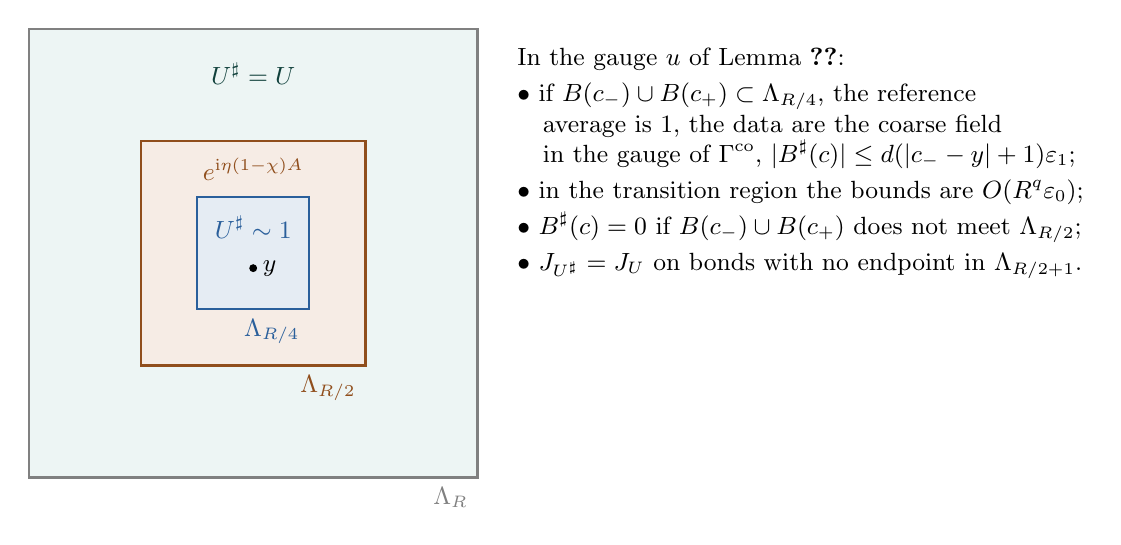
\begin{tikzpicture}[scale=0.95]
\fill[fgreen!8] (-3,-3) rectangle (3,3);
\fill[forange!12] (-1.5,-1.5) rectangle (1.5,1.5);
\fill[fblue!12] (-0.75,-0.75) rectangle (0.75,0.75);
\draw[gray,thick] (-3,-3) rectangle (3,3);
\draw[forange!80!black,thick] (-1.5,-1.5) rectangle (1.5,1.5);
\draw[fblue,thick] (-0.75,-0.75) rectangle (0.75,0.75);
\fill (0,-0.2) circle (1.5pt) node[right,font=\small] {$y$};
\node[fblue,font=\small] at (0,0.35) {$U^\sharp\sim1$};
\node[forange!80!black,font=\small] at (0,1.12) {$e^{\ii\eta(1-\chi)A}$};
\node[fgreen!50!black,font=\small] at (0,2.4) {$U^\sharp=U$};
\node[gray,font=\small,anchor=north east] at (3,-3) {$\Lam_R$};
\node[forange!80!black,font=\small,anchor=north east] at (1.5,-1.5) {$\Lam_{R/2}$};
\node[fblue,font=\small,anchor=north east] at (0.75,-0.75) {$\Lam_{R/4}$};
\node[align=left,anchor=west,font=\small] at (3.4,1.2) {In the gauge $u$ of Lemma~\ref{lem:adapted-gauge}:\\[2pt]
$\bullet$ if $B(c_-)\cup B(c_+)\subset\Lam_{R/4}$, the reference\\ \quad average is $1$, the data are the coarse field\\ \quad in the gauge of $\Gamma^{\rm co}$, $|B^\sharp(c)|\le d(|c_--y|+1)\eps_1$;\\[2pt]
$\bullet$ in the transition region the bounds are $O(R^q\eps_0)$;\\[2pt]
$\bullet$ $B^\sharp(c)=0$ if $B(c_-)\cup B(c_+)$ does not meet $\Lam_{R/2}$;\\[2pt]
$\bullet$ $J_{U^\sharp}=J_U$ on bonds with no endpoint in $\Lam_{R/2+1}$.};
\end{tikzpicture}
\caption{The spliced reference configuration of Definition~\ref{def:splice}.}
\label{fig:splice}
\end{figure}

\begin{lemma}[Splicing]\label{lem:splice}
There is $C_9\ge1$, depending only on $d$, $L$, $G$, $\alpha$ and $M$, with the following property. Let $R\ge16M+16$, and let $U$ be real and $(M,\eps_0)$-regular with $U\in\mathfrak U(\eps_0)$. Let $y$, $u$ and $A$ be as in Definition~\ref{def:splice}, with $\|A\|_{1,\alpha;\Lam_R(y)}\le s$ and $C_9(\eps_0+s)\le c_1$. Then:
\begin{enumerate}[label=(\alph*)]
\item $U^\sharp=U$ on all bonds with no endpoint in $\Lam_{R/2}(y)$, and $(U^\sharp)^u=1$ on the bonds of $\Lam_{R/4}(y)$.
\item $U^\sharp$ is $(M,C_9(\eps_0+s))$-regular, $|F_{U^\sharp}|\le C_9(\eps_0+s)$ and $|J_{U^\sharp}|\le\eps_0+C_9s$. Moreover $J_{U^\sharp}=J_U$ on bonds with no endpoint in $\Lam_{R/2+1}(y)$, and $J_{U^\sharp}=0$ on the bonds of $\Lam_{R/4-1}(y)$.
\item Let $W^\sharp=(U^\sharp)^{(k)}$ and $V=U^{(k)}$. For every bond $c$ of $\T$, $|\ell(V(c)W^\sharp(c)^{-1})|\le C_9(\eps_0+s)$. If $B(c_-)\cup B(c_+)$ does not meet $\Lam_{R/2}(y)$, then $W^\sharp(c)=V(c)$. If $B(c_-)\cup B(c_+)\subset\Lam_{R/4}(y)$, then $u(c_-)W^\sharp(c)u(c_+)^{-1}=1$.
\end{enumerate}
\end{lemma}

\begin{proof}
(a) follows from the definition, since $\chi=1$ on $\Lam_{R/4}(y)$.

(b) \emph{Regularity.} If $\Lam_{4M+2}(z)\subset\Lam_R(y)$, the gauge $u$ gives $(U^\sharp)^u=e^{\ii\eta(1-\chi)A}$ there, and $\|(1-\chi)A\|_{1,\alpha}\le Cs$ by the Leibniz rule, since $R\ge1$. Otherwise $|z-y|_\infty>R-4M-2$. Then every point of $\Lam_{4M+2}(z)$ has distance more than $R-8M-4\ge R/2$ from $y$, so $U^\sharp=U$ on $\Lam_{4M+2}(z)$, and the gauges of $U$ apply. The curvature is bounded in the same way, using $|F_{e^{\ii\eta B}}|\le C(|\partial B|+|B|^2)$.

\emph{Current.} The current at a bond depends only on the configuration on the plaquettes containing it and on their neighbours. This gives the two identities. In general, compute in the gauge $u$, which does not change $|J|$. For a configuration $e^{\ii\eta B}$ and a plaquette $p$ with bonds $b_1,\dots,b_4$ as in Definition~\ref{def:curvature},
\[
F^s_{e^{\ii\eta B}}(p)=\eta^{-2}\mathfrak S\big(\eta B(b_1),\eta B(b_2),\eta B(b_3),\eta B(b_4)\big),\qquad\mathfrak S(z)=P_{\mathfrak g}\sin\ell\big(e^{\ii z_1}e^{\ii z_2}e^{-\ii z_3}e^{-\ii z_4}\big),
\]
with $F^s$ as in Lemma~\ref{lem:current}. The function $\mathfrak S$ is analytic near $0$, and $\mathfrak S(z)=z_1+z_2-z_3-z_4+\mathfrak S_2(z)$ with $|\mathfrak S_2(z)|\le C|z|^2$ and $|\nabla\mathfrak S_2(z)|\le C|z|$. Let $t=1-\chi$ and $A^\sharp=tA$, and let $x_p$ be the base point of $p$. Then
\[
F^s_{e^{\ii\eta A^\sharp}}(p)=t(x_p)F^s_{e^{\ii\eta A}}(p)+E(p),
\]
\[
E(p)=\sum_{i=1}^4\pm\frac{t(b_i)-t(x_p)}\eta\,A(b_i)+\eta^{-2}\Big(\mathfrak S_2\big(\eta A^\sharp(b_1),\dots\big)-t(x_p)\,\mathfrak S_2\big(\eta A(b_1),\dots\big)\Big).
\]
Since $|\partial^\beta t|\le CR^{-|\beta|}$ and $|A|+|\partial A|\le s$, we get $|E|\le Cs$. Between neighbouring plaquettes, the arguments $\eta A^\sharp(b_i)$, $\eta A(b_i)$ and $t(x_p)$ change by at most $C\eta^2s$ and $C\eta/R$. With $|\nabla\mathfrak S_2(z)|\le C|z|$ and the product rule, the difference quotients of $E$ are bounded by $Cs$. By Lemma~\ref{lem:cov-expansion}, $D^T_{e^{\ii\eta B}}=\partial^*+T_B^T$ with $T_B$ local and bounded by $C|B|$. Using $J_{e^{\ii\eta A}}=D^T_{e^{\ii\eta A}}F^s_{e^{\ii\eta A}}=R(u)J_U$ (Lemma~\ref{lem:current}(a)),
\[
J_{e^{\ii\eta A^\sharp}}=t\,R(u)J_U+[\partial^*,t]F^s_{e^{\ii\eta A}}+\big(T^T_{A^\sharp}t-tT^T_A\big)F^s_{e^{\ii\eta A}}+D^T_{e^{\ii\eta A^\sharp}}E .
\]
Each term after the first is bounded by $Cs$, because $|F^s_{e^{\ii\eta A}}|\le Cs$ and $|\partial t|\le C/R$. Hence $|J_{U^\sharp}|\le\eps_0+Cs$.

(c) The average $U^{(k)}(c)$ depends only on the bonds of $B(c_-)\cup B(c_+)$ (Lemma~\ref{lem:one-step-basic}). This gives the first identity. The second follows from (a) and covariance, since $\mathfrak a^{(k)}(1)=1$; the gauge $u$ may be extended arbitrarily outside $\Lam_R(y)$. In the remaining case $B(c_-)\cup B(c_+)\subset\Lam_{R/2+2}(y)\subset\Lam_R(y)$. Lemma~\ref{lem:avg-local-gauge}, applied to $U^u$ and to $(U^\sharp)^u$ on the union of blocks $B(c_-)\cup B(c_+)$, gives $V^u(c)=e^{\ii B'}$ and $(W^\sharp)^u(c)=e^{\ii B''}$ with $|B'|\le s+32\eps_0$ and $|B''|\le s+32C'(\eps_0+s)$. Here $C'\ge1$ is the constant obtained in (b) for the curvature of $U^\sharp$. So (c) holds with $C_9\ge33(1+C')$; the same bound applies in the second case. By covariance and Lemma~\ref{lem:log-estimates}(b), $|\ell(VW^{\sharp-1})(c)|=|\ell(e^{\ii B'}e^{-\ii B''})|\le|B'|+|B''|$.
\end{proof}

\section{Localized bounds and the local improvement}\label{sec:improvement}

\subsection{Localized bounds for the relative problem}\label{ss:29.1}

Theorem~\ref{thm:variational} bounds the solution in sup norms over the whole torus. Its proof gives more. By the first-order formula and the Euler--Lagrange equation, the solution near a point is controlled by the data near that point, up to exponentially decaying contributions from far away and a quadratic error.

In the setting of Theorem~\ref{thm:variational}, let $A_*$ and $\omega$ be as there. For $y\in\T$ let $c_y=y$ be the centre of $B(y)$, and let $u_y$ be any real gauge transformation in which $U_0$ satisfies (B) on $\Lam_4(c_y)$ with parameter $C\eps$; write $\tilde A_{*,y}=R(u_y)A_*$. The bounds below hold uniformly in the choice of $u_y$. Put
\[
\mathsf b(y)=\max\{|B(c)|:\ |c_--y|_\infty\le1\},\qquad \mathsf j(y)=\max\{|J_{U_0}(b)|:\ b_-\in B(y)\},
\]
\begin{multline*}
\mathsf N(y)=|A_*|_{\Lam_1(c_y)}+|\nabla A_*|_{\Lam_1(c_y)}+|\Lap_{U_0}A_*|_{\Lam_1(c_y)}\\
+\Hol{\partial\tilde A_{*,y}}{\Lam_1(c_y)}+\max\{|\omega(c)|:\ |c_--y|_\infty\le2\},
\end{multline*}
where $c$ runs over the bonds of $\T$.

\begin{proposition}[Localized bounds]\label{prop:localized}
There are $C_7,\gamma_7>0$, independent of $k$, $n$, $\eta$ and $U_0$, such that, under the hypotheses of Theorem~\ref{thm:variational}, for every $y\in\T$:
\begin{enumerate}[label=(\alph*)]
\item $\displaystyle\mathsf N(y)\le C_7\sum_{y'\in\T}e^{-\gamma_7|y-y'|}\big(\mathsf b(y')+\mathsf j(y')\big)+C_7(\eps+\beta)^2$;
\item the configuration $U_\flat=e^{\ii\eta A_*}U_0$, which is gauge equivalent to the minimizer $U_*$, satisfies
\[
|F_{U_\flat}(p)|\le|F_{U_0}(p)|+C_7\mathsf N(y),\qquad|J_{U_\flat}(b)|\le C_7\mathsf N(y)
\]
for all plaquettes $p$ and bonds $b$ with base point in $B(y)$.
\end{enumerate}
\end{proposition}

\begin{proof}
Throughout, sums of products of exponentially decaying kernels are again exponentially decaying, with a smaller rate; $\gamma_7$ is the rate obtained at the end. We use the pointwise bounds of Parts~II and~III at $U_0$, which hold by Corollary~\ref{cor:parts-apply}, on cubes $\Lam_1(z)$ instead of blocks (Remark~\ref{rem:cubes}).

\emph{Step 1: first derivatives.} By Theorem~\ref{thm:variational}(c), $A_*=\bH B-\bC J_{U_0}+\mathcal R$ with $|\mathcal R|_{C^1}\le C(\eps+\beta)^2$. By the pointwise bounds of Theorem~\ref{thm:reg-min} (Theorem~\ref{thm:cov-min}(b),(d)),
\[
\begin{aligned}
|\bH B|_{\Lam_1(c_y)}+|\nabla\bH B|_{\Lam_1(c_y)}&\le C\sum_{y'}e^{-\gamma|y-y'|}\mathsf b(y'),\\
|\bC J_{U_0}|_{\Lam_1(c_y)}+|\nabla\bC J_{U_0}|_{\Lam_1(c_y)}&\le C\sum_{y'}e^{-\gamma|y-y'|}\mathsf j(y').
\end{aligned}
\]
Let $\mathsf N_1(y)=|A_*|_{\Lam_1(c_y)}+|\nabla A_*|_{\Lam_1(c_y)}$. Then $\mathsf N_1(y)$ is bounded by the right-hand side of (a).

\emph{Step 2: the multiplier.} By the proof of Proposition~\ref{prop:euler-lagrange}, for every bond $c$ of $\T$ and $\beta_0\in\mathfrak g$ with $|\beta_0|=1$,
\[
\operatorname{tr}(\beta_0\,\omega(c))=\ip\varphi{J_{U_0}+\nabla\mathcal N(A_*)}+\ip{D\varphi}{DA_*},
\]
with $|\varphi(x)|+|\nabla\varphi(x)|\le Ce^{-\gamma'|x-c_-|}$. Moreover $|\nabla\mathcal N(A_*)|_\infty\le C(\eps+|A_*|_\infty)|A_*|_{C^1}\le C(\eps+\beta)^2$ by Proposition~\ref{prop:action}(a). Hence
\[
|\omega(c)|\le C\sum_{y'}e^{-\gamma'|c_--y'|}\big(\mathsf j(y')+\mathsf N_1(y')\big)+C(\eps+\beta)^2 .
\]

\emph{Step 3: second order.} By Propositions~\ref{prop:action} and~\ref{prop:euler-lagrange},
\[
D^TDA_*=d\mathcal Q(A_*)^T\omega-J_{U_0}-\nabla\mathcal N(A_*).
\]
By Proposition~\ref{prop:Q-expansion}(c), the kernel of $d\mathcal Q(A_*)^T=\bQ^T+d\Cav_k(A_*)^T$ connects a bond $b$ only to bonds $c$ with $b_-\in S_c$. Hence $|d\mathcal Q(A_*)^T\omega|_{\Lam_1(c_y)}\le C\max\{|\omega(c)|:|c_--y|_\infty\le2\}$. Since $RD^TA_*=0$, we have $\Lap_{U_0}A_*=D^TDA_*+DP_\cV D^TA_*$. The second term is bounded on $\Lam_1(c_y)$ by $C\sum_{y'}e^{-\gamma|y-y'|}|A_*|_{B(y')}$, by the pointwise bound on $\partial P_\cV D^T$ in Proposition~\ref{prop:cov-R}(e) (Theorem~\ref{thm:reg-scalar}(g)) and $D=\partial+T$. This bounds $|\Lap_{U_0}A_*|_{\Lam_1(c_y)}$. For the H\"older quotient, write $\Lap_{U_0}$ in the gauge $u_y$ in the normal form of Lemma~\ref{lem:cov-expansion}. Then $-\Lap\tilde A_{*,y}=R(u_y)\Lap_{U_0}A_*-\sum_\mu\partial^*_\mu(a_\mu\tilde A_{*,y})-b\tilde A_{*,y}$ on $\Lam_3(c_y)$, with $|a_\mu|+[a_\mu]_\alpha+|b|\le C\eps$. Theorem~\ref{thm:local-regularity}(d) gives
\[
\Hol{\partial\tilde A_{*,y}}{\Lam_1(c_y)}\le C\Big(|\Lap_{U_0}A_*|_{\Lam_2(c_y)}+\max_{|y'-y|_\infty\le3}\mathsf N_1(y')\Big).
\]
The cube $\Lam_2(c_y)$ is covered by the cubes $\Lam_1(c_{y'})$ with $|y'-y|_\infty\le1$; the values of $\omega$ that enter there are bounded by Step~2 for all bonds. Combining Steps 1--3 gives (a).

(b) By \eqref{eq:plaquette-product}, $U_\flat(\partial p)=e^{\ii\eta^2\zeta_p(A_*)}U_0(\partial p)$ with $|\zeta_p(A_*)|\le C(|A_*|+|\nabla A_*|)$ on the bonds of $p$. Lemma~\ref{lem:log-estimates}(b) gives the bound on the curvature. By Proposition~\ref{prop:action}(d) and Proposition~\ref{prop:euler-lagrange}, $J_{U_\flat}=\Psi(A_*)^{-T}d\mathcal Q(A_*)^T\omega$. As in Step 3, this is bounded at $b$ by $C\max\{|\omega(c)|:|c_--y|_\infty\le2\}$.
\end{proof}

\subsection{The local improvement}\label{ss:29.2}

\begin{lemma}[Local improvement]\label{lem:improvement}
There are $\eps_{\rm imp}>0$, $C_{\rm imp}\ge1$ and an integer $n_0$, depending only on $d$, $L$, $G$, $a$, $\alpha$ and $M$, with the following property. Let $k\ge1$, $n\ge n_0$, and let $V\in\mathfrak U_k(\eps_1)$ be a real configuration on $\T$. Let $U\in\mathfrak B(V)$ be a critical point of $S|_{\mathfrak B(V)}$. Suppose that $U$ is $(M,\eps_0)$-regular and $U\in\mathfrak U(\eps_0)$, with $\eps_0\le\eps_{\rm imp}$. Then $U$ is $(M,\eps_0')$-regular and $U\in\mathfrak U(\eps_0')$, where
\[
\eps_0'=C_{\rm imp}\eps_1+\tfrac12\eps_0 .
\]
If $\eps_0'>1$, the regularity conclusion is read as $(M,1)$-regularity; it gives the three bounds of Definition~\ref{def:regular} with $\eps_0'$ in place of $\eps$.
\end{lemma}

The point is that $C_{\rm imp}$ does not depend on $\eps_0$. Iterating the lemma brings the regularity parameter down to $2C_{\rm imp}\eps_1$, whatever the a priori bound, as long as the latter is at most $\eps_{\rm imp}$.

\begin{proof}
If $\eps_1>2\eps_0$ there is nothing to prove, since then $\eps'_0\ge\eps_0$. So let $\eps_1\le2\eps_0$.

\emph{Choice of constants.} Let $C_7,\gamma_7$ be as in Proposition~\ref{prop:localized}, $C_8,q$ as in Lemma~\ref{lem:adapted-gauge}, and $C_9$ as in Lemma~\ref{lem:splice}. Put
\[
K_R=2C_9\big(1+C_8R^q\big),\qquad S_1=\sum_{w\in\Z^d}e^{-\gamma_7|w|}(1+|w|),\qquad T(t)=\sum_{w\in\Z^d,\,|w|_\infty>t}e^{-\gamma_7|w|},
\]
and $K_1=\max(5,C_7)$. Fix an integer $R\ge64(M+1)$ with
\[
K_1C_7K_R\,T(R/8)\le\tfrac14 ;
\]
this is possible because $K_R$ grows polynomially and $T$ decays exponentially. Let $n_0=4R+16$. Choose $\eps_{\rm imp}$ so small that $K_1C_7K_R^2\eps_{\rm imp}\le\frac14$, $K_R\eps_{\rm imp}\le c_6$, $\eps_{\rm imp}\le\theta_0$, $C_8R^q\eps_{\rm imp}\le1$ and $C_9(1+C_8R^q)\eps_{\rm imp}\le c_1$.

\emph{Step 1: the adapted gauge.} Fix $y\in\T$. By Lemma~\ref{lem:adapted-gauge} there is a real gauge transformation $u$ on $\Lam_R(y)$ with $U^u=e^{\ii\eta A}$, $\|A\|_{1,\alpha;\Lam_R(y)}\le s:=C_8R^q\eps_0$, and $V^u(c)=e^{\ii B_y(c)}$ with $|B_y(c)|\le d(|c_--y|_\infty+1)\eps_1$ for the bonds of $\T$ in $\Lam_R(y)$.

\emph{Step 2: the spliced reference.} Let $U^\sharp$ be the spliced configuration of Definition~\ref{def:splice}, built with this $u$. By Lemma~\ref{lem:splice}, $U^\sharp$ is $(M,\eps^\sharp)$-regular with $|J_{U^\sharp}|\le\eps^\sharp$, where $\eps^\sharp=C_9(\eps_0+s)$. Moreover $V(c)W^\sharp(c)^{-1}=e^{\ii B^\sharp(c)}$ with $|B^\sharp|_\infty\le\beta^\sharp:=C_9(\eps_0+s)$, where $W^\sharp=(U^\sharp)^{(k)}$. Then $\eps^\sharp+\beta^\sharp\le K_R\eps_0\le c_6$. So Theorem~\ref{thm:variational} applies with the reference $U^\sharp$ and the coarse configuration $V$.

\emph{Step 3: identification.} By Theorem~\ref{thm:variational}(a), $S|_{\mathfrak B(V)}$ has exactly one critical orbit in $\mathfrak B(V)\cap\mathfrak U(\theta_0)$. Since $U$ is critical and lies in $\mathfrak U(\eps_0)\subset\mathfrak U(\theta_0)$, it belongs to this orbit. Hence $U=(e^{\ii\eta A^\sharp_*}U^\sharp)^v$ for a real gauge transformation $v$, where $A^\sharp_*$ is the Landau representative relative to $U^\sharp$. Applying $u$, we get on the bonds of $\Lam_{R/4}(y)$, where $(U^\sharp)^u=1$,
\[
U^{uv^{-1}}=e^{\ii\eta\tilde A},\qquad\tilde A=R(u)A^\sharp_* .
\]
In this gauge $\nabla_{U^\sharp}$ is the ordinary difference, and $u$ is a gauge in which $U^\sharp$ satisfies (B) near every block in $\Lam_{R/4-4}(y)$.

\emph{Step 4: the data near $y$.} Apply Proposition~\ref{prop:localized} with reference $U^\sharp$. Let $y'\in\T$ with $|y'-y|_\infty\le R/4-3$. Every bond $c$ with $|c_--y'|_\infty\le1$ has $B(c_-)\cup B(c_+)\subset\Lam_{R/4}(y)$. So, by Lemma~\ref{lem:splice}(c), $(W^\sharp)^u(c)=1$, and
\[
|B^\sharp(c)|=|\ell(V^u(c))|=|B_y(c)|\le d(|y'-y|_\infty+2)\eps_1 .
\]
Moreover $\mathsf j(y')=0$ by Lemma~\ref{lem:splice}(b). For the remaining $y'$ we only use $\mathsf b(y')+\mathsf j(y')\le K_R\eps_0$. Let $y_1\in\T$ with $|y_1-y|_\infty\le4M+4$. For $|y'-y|_\infty>R/4-3$ we have $|y_1-y'|_\infty>R/8$, because $R\ge64(M+1)$. Therefore
\[
\mathsf N(y_1)\le C_7dS_1(4M+7)\,\eps_1+C_7K_R\,T(R/8)\,\eps_0+C_7K_R^2\eps_0^2 .
\]

\emph{Step 5: conclusion.} Let $z\in\Tf$, and choose $y\in\T$ with $|z-y|_\infty\le1$. Then $\Lam_{4M+2}(z)\subset\Lam_{4M+3}(y)\subset\Lam_{R/4-4}(y)$. By Step 3, $U^{uv^{-1}}=e^{\ii\eta\tilde A}$ on $\Lam_{4M+2}(z)$. On it, $|\tilde A|$, $|\partial\tilde A|$ and the H\"older quotients of $\partial\tilde A$ on cubes $\Lam_1(c_{y_1})$ are bounded by $\mathsf N(y_1)$, with the gauge $u_{y_1}=u$. Put $H=\max_{|y_1-y|_\infty\le4M+4}\mathsf N(y_1)$. Let $x\ne x'$ be points of a cube $\Lam_3(z')\subset\Lam_{4M+2}(z)$. If $|x-x'|_\infty<\frac12$, then in each coordinate $x$ and $x'$ differ by a multiple of $\eta=1/N$ less than $\frac12$, hence by at most $\frac{N-1}{2N}$, since $N$ is odd. A difference involves points at most $2\eta$ beyond its base point in each coordinate (for $\partial_\mu\tilde A_\mu$, the point $x+2\eta e_\mu$). So the points of the two differences span, in each coordinate, an interval of length at most $\frac{N-1}{2N}+\frac2N=\frac{N+3}{2N}\le1$, since $N\ge3$. The centres $c$ with $|p-c|_\infty\le1$ for all these points $p$ form, in each coordinate, a closed interval of length at least $1$. The block centres form a grid of spacing $1$, so one of them lies in it: these points lie in a common cube $\Lam_1(c_{y_1})$, and then $|y_1-y|_\infty\le4M+4$. If $|x-x'|_\infty\ge\frac12$, the H\"older quotient is at most $4\sup|\partial\tilde A|$. Hence $|\tilde A|\le H$, $|\partial\tilde A|\le H$, and the H\"older quotients of $\partial\tilde A$ on the cubes $\Lam_3(z')\subset\Lam_{4M+2}(z)$ are at most $4H$. These are the three bounds of Definition~\ref{def:regular}, and each is at most $K_1H$, since $K_1\ge5$. By Proposition~\ref{prop:localized}(b), with $F_{U^\sharp}=0$ near $y$, the curvature and the current of $U$ on the plaquettes and bonds based in $B(y)$ are bounded by $C_7\mathsf N(y)$. All these quantities are gauge invariant. Every plaquette and bond is based in some block, and every $z$ is close to some $y$. With the choice of $R$ and $\eps_{\rm imp}$, Step~4 gives the lemma with $C_{\rm imp}=K_1C_7dS_1(4M+7)$:
\[
K_1\max\mathsf N\le C_{\rm imp}\eps_1+\tfrac14\eps_0+\tfrac14\eps_0 .\qedhere
\]
\end{proof}

\begin{remark}[Comparison with {\cite[Sect.~F]{BalVar}}]\label{x:29.3}
The structure of the argument is Ba\l aban's: near a point the minimizer equals, up to small errors, $\bH$ applied to the coarse field in a gauge centred at the point (for us the gauge of the contours $\Gamma^{\rm co}$ of Section~\ref{sec:local-gauges}); the latter grows only linearly with the distance, with slope given by the curvature of $V$, while $\bH$ decays exponentially. Compare \cite[(159)--(167)]{BalVar}. The difference is in how the problem is localized. Ba\l aban formulates a new variational problem on a nested sequence of cubes around the point. The configuration is frozen outside, and the problem is solved relative to the trivial configuration. Here the problem is not changed. Only the reference configuration is changed, and Theorem~\ref{thm:variational} is applied once more on the torus. This is possible because that theorem is uniform in the reference. The splicing is a purely geometric operation (Lemma~\ref{lem:splice}). As in \cite[(166)]{BalVar}, the quadratic error forces the a priori bound to be small in terms of the localization radius.
\end{remark}

\section{The induction over the number of steps}\label{sec:induction}

We now prove Ba\l aban's variational theorem on the torus by induction over $k$. Each step has three parts:
\begin{itemize}
\item the solution of the $(k-1)$-step problem for the trivial extension of $V$ is a reference with \emph{exactly} the right averages \cite[Sect.~A]{BalVar};
\item Theorem~\ref{thm:variational} solves the problem near this reference, with an a priori regularity bound that is worse by a power of $L$;
\item Lemma~\ref{lem:improvement}, iterated, restores the regularity bound with a constant independent of $k$.
\end{itemize}

\subsection{The trivial extension}\label{ss:30.1}

Let $k\ge1$. A bond $b$ of $\T^{(k-1)}$ in direction $\mu$ is a \emph{crossing bond} if its endpoints lie in different blocks, $b_-\in B_k(y)$ and $b_+\in B_k(y+e_\mu)$; we then write $c(b)=(y,y+e_\mu)$. For a configuration $V$ on $\T$ define $V_0$ on $\T^{(k-1)}$ by
\[
V_0(b)=V(c(b))\ \text{ for crossing bonds},\qquad V_0(b)=1\ \text{ for bonds inside a block}
\]
\cite[(11)]{BalVar}.

\begin{lemma}[Trivial extension]\label{lem:trivial-extension}
\begin{enumerate}[label=(\alph*)]
\item $\mathfrak a_k(V_0)=V$.
\item Let $p$ be a plaquette of $\T^{(k-1)}$. If $p$ has crossing bonds in both of its directions, then $V_0(\partial p)=V(\partial p')$, where $p'$ is the plaquette of $\T$ spanned by the four blocks containing the corners of $p$. Otherwise $V_0(\partial p)=1$. Hence $F_{V_0}(p)=L^2F_V(p')$ or $0$, and $V\in\mathfrak U_k(\eps_1)$ implies $V_0\in\mathfrak U_{k-1}(L^2\eps_1)$.
\end{enumerate}
\end{lemma}

\begin{proof}
(a) Let $c=(y,y+e_\mu)$ and $x\in B_k(y)$. Every contour of the family $G(y,x)$ lies in the box spanned by $y$ and $x$, which is contained in $B_k(y)$. So it consists of bonds inside a block, on which $V_0=1$. The family $\{V_0(\Gamma)\}_{\Gamma\in G(y,x)}$ is therefore the constant family $\{1,\dots,1\}$, and $V_0(y,x)=1$ by Lemma~\ref{lem:group-average}(b). Likewise $V_0(y+e_\mu,x(c))=1$. Write $x_\mu=y_\mu+m\delta_{k-1}$ with $|m|\le\frac{L-1}2$. The straight contour $[x,x(c)]$ has $L$ bonds in direction $\mu$, starting at the points with $\mu$-coordinates $y_\mu+i\delta_{k-1}$, $m\le i\le m+L-1$. Exactly one of them, the one with $i=\frac{L-1}2$, joins $B_k(y)$ to $B_k(y+e_\mu)$; it is a crossing bond $b$ with $c(b)=c$, and the others lie inside a block. The same holds for $[c]$, which is the case $m=0$. Hence $V_0([x,x(c)])=V(c)=V_0([c])$. So every averaged loop is $\Lambda_{c,x}(V_0)=1\cdot V(c)\cdot1\cdot V(c)^{-1}=1$, all logarithms in \eqref{eq:one-step} vanish, and $\mathfrak a_k(V_0)(c)=V_0([c])=V(c)$. For the reversed bond $-c$ the claim follows from Lemma~\ref{lem:reversal}.

(b) The two bonds of $p$ in direction $\mu$ are crossing or not simultaneously, and they connect the same pair of blocks if the bonds in direction $\nu$ do not cross. In that case $V_0(\partial p)$ is $V(c)V(c)^{-1}=1$ or $1$. If both pairs cross, the four bonds carry the values of $V$ on the four bonds of $\partial p'$, in the order of Definition~\ref{def:curvature}. Finally $F_{V_0}(p)=\delta_{k-1}^{-2}\ell(V_0(\partial p))=L^2\ell(V(\partial p'))=L^2F_V(p')$.
\end{proof}

In units of $\delta_{k-1}$, curvatures are multiplied by $\delta_{k-1}^2=L^{-2}$. So in its own units, $V_0$ satisfies the same curvature bound $\eps_1$ as $V$.

\subsection{Change of units}\label{ss:30.2}

As in the proof of Theorem~\ref{thm:chart}, the $(k-1)$-step structure on $(\Tf,\T^{(k-1)})$, in units of $\delta_{k-1}$, is the $(k-1)$-step structure on a torus of side $Ln$ with fine spacing $L\eta$. The Wilson action does not change, since $d=4$ (Section~\ref{sec:action}); so critical points and minimizers are the same.

\begin{lemma}[Change of units]\label{lem:units}
There is $C^{\rm units}_L$, depending only on $d$, $\alpha$, $G$, $L$ and $M$, with the following property. Let $U_0$ be a real configuration on $\Tf$ which, in units of $\delta_{k-1}$, lies in $\mathfrak U(\theta)$ and is $(M,\theta)$-regular. If $C^{\rm units}_L\theta\le1$, then in units of $\delta_k=1$, $U_0\in\mathfrak U(L^3\theta)$ and $U_0$ is $(M,C^{\rm units}_L\theta)$-regular.
\end{lemma}

\begin{proof}
Passing to units of $\delta_k$ divides lengths by $L$ and multiplies Lie fields by $L$, their differences and curvatures by $L^2$, currents by $L^3$, and H\"older quotients of differences by $L^{2+\alpha}$. This gives the first claim. For the second, let $r'=(4M+2)/L$. Every cube $\Lam_{r'}(z)$ carries a gauge with $|A|\le L\theta$ and $|\partial A|\le L^2\theta$, and with H\"older quotients of $\partial A$ at most $L^{2+\alpha}\theta$ on cubes of radius $3/L$. Let $r=r'-2$. Two points of $\Lam_r(z)$ at distance at most $3/L$ lie in a common cube of radius $3/L$ contained in $\Lam_{r'}(z)$. For points at larger distance the quotient is at most $2|\partial A|(L/3)^\alpha$. Hence $U_0$ is $3L^3\theta$-regular on every cube $\Lam_r(z)$. Since $M\ge5L$, $r\ge18$. Lemma~\ref{lem:large-cubes} with $R=4M+2$ gives the claim, with $C^{\rm units}_L=3C_E(4M+2)^{p+1}L^3$.
\end{proof}

\subsection{The theorem}\label{ss:30.3}

\begin{theorem}[Ba\l aban's variational theorem on the torus]\label{thm:balaban}
Assume the conventions of Part~VI, in particular $M\ge\max(M_0,5L)$. Let $\theta_0$ be as in Theorem~\ref{thm:variational} and $n_0$ as in Lemma~\ref{lem:improvement}. There are $a_1,B_3>0$, depending only on $d$, $L$, $G$, $a$, $\alpha$ and $M$, such that the following holds for all $k\ge0$, all $n\ge n_0$ and every real configuration $V$ on $\T$ with $V\in\mathfrak U_k(\eps_1)$, $\eps_1\le a_1$.
\begin{enumerate}[label=(\alph*)]
\item $S|_{\mathfrak B(V)}$ has exactly one critical orbit in $\mathfrak B(V)\cap\mathfrak U(\theta_0)$. This orbit is the set of minimizers of $S$ on $\mathfrak B(V)\cap\mathfrak U(\theta_0)$.
\item Every element $U_k(V)$ of this orbit lies in $\mathfrak U(B_3\eps_1)$ and is $(M,B_3\eps_1)$-regular.
\item \emph{(Lattice symmetry.)} For $r\in\mathfrak S_k$, $rV\in\mathfrak U_k(\eps_1)$, and the minimal orbit of $rV$ is the image under $r$ of the minimal orbit of $V$. In particular $S(U_k(rV))=S(U_k(V))$.
\end{enumerate}
The constants do not depend on $k$, $n$ or $\eta$.
\end{theorem}

This is \cite[Theorem~1]{BalVar} for a single torus with the small-field condition everywhere. Part~(b) is the regularity statement \cite[(8)--(10)]{BalVar} for cubes of the fixed size $M$. As in \cite{BalVar}, the elements of the orbit are called \emph{background fields} or \emph{minimal configurations}.

\begin{proof}\hasdetail{thm:balaban}
\emph{Constants.} Let $C_{\rm base}$ be the constant of the case $k=0$ below, and put
\[
B_3=\max(4C_{\rm imp},C_{\rm base}),\qquad K=(1+C_6)C^{\rm units}_L .
\]
Choose $a_1$ so small that $C^{\rm units}_LB_3a_1\le\min(c_6,1)$, $KB_3a_1\le\eps_{\rm imp}$, $B_3a_1\le\theta_0$, $a_1\le c_1$, $d(8M+6)a_1\le c_G$, and $B_3a_1\le c'_3$, with $c'_3$ of Section~\ref{sec:AB-proof}, which depends only on $d$, $L$ and $G$. The last condition is used only in Part~XI, where Proposition~\ref{prop:AB} is applied at the background fields of arbitrary small-field configurations (proof of Theorem~\ref{thm:ol-chart}). These choices do not depend on $k$.

\emph{The case $k=0$.} Then $\eta=1$, $\Tf=\T$, $\mathfrak B(V)=\{V\}$ and $\mathfrak G_0=\{1\}$. We first prove (b); then $V\in\mathfrak U(B_3\eps_1)\subset\mathfrak U(\theta_0)$, and (a) is trivial. The current $J_V=D^T_VF^s_V$ is a combination of at most $4d$ values of $F^s_V$, so $|J_V|\le C\eps_1$. For regularity, fix $z$ and a point $z_0\in\T$ with $|z-z_0|_\infty\le1$, and let $u$ be the gauge on $\Lam_{4M+2}(z)$ with $V^u(\Gamma^{\rm co}_{z_0,x})=1$, with the contours $\Gamma^{\rm co}$ of Section~\ref{sec:local-gauges} (here the fine and the unit lattice coincide). As in the proof of Lemma~\ref{lem:adapted-gauge}, $|\ell(V^u(b))|\le d(4M+4)\eps_1$ for every bond $b$ of $\Lam_{4M+2}(z)$. On the unit lattice, for $A=\ell(V^u)$, $|\partial A|\le2|A|$, and the H\"older quotients of $\partial A$ are at most $2|\partial A|\le4|A|$, since distinct points have distance at least $1$. So $V$ is $(M,C_{\rm base}\eps_1)$-regular and lies in $\mathfrak U(C_{\rm base}\eps_1)$, with $C_{\rm base}$ depending only on $d$, $G$ and $M$.

\emph{From $k-1$ to $k$.} Let $V\in\mathfrak U_k(\eps_1)$ with $\eps_1\le a_1$, and let $V_0$ be its trivial extension. In units of $\delta_{k-1}$ the torus has side $Ln\ge n_0$, and $V_0$ has curvature at most $\eps_1$ (Lemma~\ref{lem:trivial-extension}). By the induction hypothesis there is a minimal configuration $U_0=U_{k-1}(V_0)$. In units of $\delta_{k-1}$ it lies in $\mathfrak U(B_3\eps_1)$ and is $(M,B_3\eps_1)$-regular. By Lemma~\ref{lem:units}, in units of $\delta_k$,
\[
U_0\in\mathfrak U(L^3B_3\eps_1),\qquad U_0\ \text{is}\ (M,\eps)\text{-regular},\qquad\eps:=C^{\rm units}_LB_3\eps_1\le c_6 .
\]
Since $U_0^{(k-1)}=V_0$, Lemma~\ref{lem:trivial-extension}(a) gives
\[
W_k=U_0^{(k)}=\mathfrak a_k(V_0)=V ,
\]
so the hypotheses of Theorem~\ref{thm:variational} hold with $\beta=0$; note $|J_{U_0}|\le L^3B_3\eps_1\le\eps$. Parts (a) and (b) of that theorem give (a).

For (b), let $U$ be an element of the orbit. By Theorem~\ref{thm:variational}(e), $U$ is $(M,\eps_0^{(0)})$-regular and lies in $\mathfrak U(\eps_0^{(0)})$, with $\eps_0^{(0)}=(1+C_6)\eps=KB_3\eps_1\le\eps_{\rm imp}$. If $\eps_0^{(0)}\le B_3\eps_1$ there is nothing to prove, so let $\eps_0^{(0)}>B_3\eps_1\ge4C_{\rm imp}\eps_1$. Define $\eps_0^{(m+1)}=C_{\rm imp}\eps_1+\frac12\eps_0^{(m)}$. If $\eps_0^{(m)}\ge2C_{\rm imp}\eps_1$, then $\eps_0^{(m+1)}\le\eps_0^{(m)}$. By Lemma~\ref{lem:improvement} and induction over $m$, $U$ is $(M,\eps_0^{(m)})$-regular and lies in $\mathfrak U(\eps_0^{(m)})$ for all $m$. Since
\[
\eps_0^{(m)}-2C_{\rm imp}\eps_1=2^{-m}\big(\eps_0^{(0)}-2C_{\rm imp}\eps_1\big)\le2^{-m}KB_3\eps_1 ,
\]
we have $\eps_0^{(m)}\le2C_{\rm imp}\eps_1+\frac12B_3\eps_1\le B_3\eps_1$ once $2^{m}\ge2K$. This proves (b) with the same $B_3$, and closes the induction.

\emph{Part (c).} The set $\mathfrak U_k(\eps_1)$ is invariant under $\mathfrak S_k$ (Section~\ref{sec:averaging}). As in the proof of Theorem~\ref{thm:variational}(h), the map $U\mapsto rU$ maps $\mathfrak B(V)\cap\mathfrak U(\theta_0)$ onto $\mathfrak B(rV)\cap\mathfrak U(\theta_0)$, preserves $S$ and its critical points, and maps $\mathfrak G_0$-orbits onto $\mathfrak G_0$-orbits. So it maps the critical orbit of (a) for $V$ onto that for $rV$. Since $S$ is constant on this orbit and $S\circ r=S$, the last claim follows.
\end{proof}

The induction uses Theorem~\ref{thm:variational} with $\beta=0$: the reference has exactly the prescribed averages. On the nested domains of \cite{BalVar} this is not the case, and $\beta$ is of order $\eps_1$ \cite[(14)]{BalVar}. Theorem~\ref{thm:variational} allows $\beta>0$, which is used in Lemma~\ref{lem:improvement} and in Corollary~\ref{cor:analytic} below.

\subsection{Consequences}\label{ss:30.4}

\begin{corollary}[Local regularity from gauge-invariant conditions]\label{cor:regularity}
There are $a_2,B_5>0$, depending only on $d$, $L$, $G$, $a$, $\alpha$ and $M$, such that for all $k\ge0$ and $n\ge n_0$ every real configuration $U\in\mathfrak U(\theta)$ on $\Tf$ with $\theta\le a_2$ is $(M,B_5\theta)$-regular. More precisely, $U$ is gauge equivalent, by a real gauge transformation, to $e^{\ii\eta A}U_k(U^{(k)})$. Here $A$ lies in Ba\l aban's Landau gauge relative to $U_k(U^{(k)})$, and $A$ obeys the bounds of Theorem~\ref{thm:chart} with $\eps+\theta+\beta=(2B_3+1)\theta$.
\end{corollary}

\begin{proof}
Let $k=0$. Then $\eta=1$, $\Tf=\T$ and $U^{(0)}=U$. By the case $k=0$ of the proof of Theorem~\ref{thm:balaban}, $\mathfrak B(U)=\{U\}$, so $U_0(U)=U$, and the representation holds with $A=0$, for which the gauge condition and the bounds are trivial. The curvature of $U$ is at most $\theta\le a_1$, so Theorem~\ref{thm:balaban}(b), with $V=U$ and $\eps_1=\theta$, shows that $U$ is $(M,B_3\theta)$-regular.

Let $k\ge1$ and $V=U^{(k)}$. By Proposition~\ref{prop:avg-regular}, $V\in\mathfrak U_k(2\theta)$. Let $2\theta\le a_1$ and $(2B_3+1)\theta\le c_4$. By Theorem~\ref{thm:balaban}, $U_0=U_k(V)$ exists. It is $(M,2B_3\theta)$-regular, satisfies $|J_{U_0}|\le2B_3\theta$, and has $U_0^{(k)}=V$. Since $U\in\mathfrak U_0(c_1)$ and $U_0\in\mathfrak U_0(2B_3\theta)\subset\mathfrak U_0(c_1)$, Lemma~\ref{lem:axial}(c) applies: the $\mathfrak G_0$-orbit of $U$ contains its averaged axial representative $U^{\rm ax}$, with $U'=U^{\rm ax}U_0^{-1}\in\mathrm{Ax}_k$. Transformations in $\mathfrak G_0$ do not change the averages, so $U'^{[k]}=(U^{\rm ax})^{(k)}V^{-1}=1$. Theorem~\ref{thm:chart}, with $\eps=2B_3\theta$ and $\beta=0$, gives $\tilde U=e^{\ii\eta A}$ in the Landau gauge with $(\tilde UU_0)^{\mathsf w_k(\tilde U)}=U^{\rm ax}$ and with the stated bounds. Finally, $e^{\ii\eta A}U_0$ is $(M,2B_3\theta+CB_1(2B_3+1)\theta)$-regular, by the argument in the proof of Proposition~\ref{prop:minimizer-regularity}(c). That argument uses the H\"older bound on the unit cubes $\Lam_1(z)$. For the field $A$ of Theorem~\ref{thm:chart} this bound is given by the proof of Proposition~\ref{prop:a-priori} (Theorem~\ref{thm:local-regularity}(d)) and Remark~\ref{rem:cubes}. So the corollary holds with $B_5=2B_3+CB_1(2B_3+1)$, which is at least the constant $B_3$ of the case $k=0$.
\end{proof}

Corollary~\ref{cor:regularity} is the torus version of \cite[Sect.~F, Prop.~6]{BalReg} and of the regularity conditions \cite[(3.35)--(3.36)]{BalBackground}. It removes the hypothesis of Part~III for all configurations of Ba\l aban's small-field class: on tori of side $n\ge n_0$, regularity follows from the gauge-invariant bounds on curvature and current. The proof uses the background field as a reference: the local gauges are the Landau gauge relative to $U_k(U^{(k)})$, composed with the local gauges of the background field. The latter come out of the induction.

\begin{corollary}[Analyticity around a background field {\cite[Sect.~G]{BalVar}}]\label{cor:analytic}
Let $V$ be as in Theorem~\ref{thm:balaban}, and let $U_0$ be an element of its minimal orbit. For $k\ge1$, Theorem~\ref{thm:variational} applies with this reference and $\eps=B_3\eps_1$. For real $B$ on $\T$ with $|B|_\infty\le\beta$ and $B_3\eps_1+\beta\le c_6$, the critical orbit for $e^{\ii B}V$ in $\mathfrak B(e^{\ii B}V)\cap\mathfrak U(\theta_0)$ is unique, and its Landau representative $A_*(B)$ relative to $U_0$ satisfies $A_*(0)=0$. The map $B\mapsto A_*(B)$ extends analytically to complex $B$, and $dA_*(B)\delta B$ decays exponentially away from the support of $\delta B$, as in Theorem~\ref{thm:variational}(f). For $r\in\mathfrak S_k$, $rU_0$ is an element of the minimal orbit of $rV$, and $A_*(r_VB;rU_0)=r_{U_0}A_*(B;U_0)$, the second argument being the reference.
\end{corollary}

\begin{proof}
$U_0$ is $(M,B_3\eps_1)$-regular with $|J_{U_0}|\le B_3\eps_1$, and $W_k=V$. For $B=0$, the configuration $U_0=\mathsf U(0)$ is critical, and $A=0$ lies in the Landau gauge with $\mathcal Q(1)=1$; by uniqueness, $A_*(0)=0$. For $k\ge1$, the symmetry statement follows from Theorem~\ref{thm:balaban}(c) and Theorem~\ref{thm:variational}(h), since $W_k=V$, and the rest is Theorem~\ref{thm:variational}.

Let $k=0$. The operators of Parts~II--V need $k\ge1$ (Section~\ref{sec:setup}), but the conclusions hold directly. Here $\eta=1$, $\Tf=\T$, $\mathfrak G_0=\{1\}$ and $U_0=V$, by the case $k=0$ of the proof of Theorem~\ref{thm:balaban}. The averaging, the correspondence transformation and $\mathcal Q$ are the identity, so $\mathfrak B(e^{\ii B}V)=\{e^{\ii B}V\}$, and the relative field of $e^{\ii B}V$ is $A_*(B)=B$; the Landau gauge condition is void. By Lemma~\ref{lem:log-estimates}(b), the curvature of $e^{\ii B}V$ is at most $\eps_1+4|B|_\infty$, and its current, a combination of at most $4d$ values of $F^s$, is at most $4d$ times this. Since $\eps_1\le B_3\eps_1$, both are at most $20d\,c_6\le\min(\theta_0,c_1)$, by the choice of $c_6$ in the proof of Theorem~\ref{thm:variational}. So the configuration $e^{\ii B}V$ lies in $\mathfrak U(\theta_0)\cap\mathfrak U_0(c_1)$, and its orbit is the unique critical orbit. The map $B\mapsto B$ is entire, $A_*(0)=0$, and $|A_*(B)|_{C^1}\le3|B|_\infty$ by \eqref{eq:lattice-trick}. Finally $dA_*(B)\delta B=\delta B$ is supported on the bond $c$, and its covariant gradient on the bonds within distance $1$ of $c$. This is the decay of Theorem~\ref{thm:variational}(f), with $C_6\ge3e^{\gamma'}$. For $r\in\mathfrak S_0$, $rU_0=rV$ is the element of the minimal orbit of $rV$ (Theorem~\ref{thm:balaban}(c)), and $A_*(r_VB;rU_0)=r_VB=r_{U_0}A_*(B;U_0)$, since $U_0=V$.
\end{proof}

\begin{remark}[Cubes of size of order $\eps_1^{-1}$]\label{rem:large-cubes}
Ba\l aban also proves gauges on cubes of side $2M'\le c\,\eps_1^{-1}$, with bounds $B_3M'\eps_1$ linear in the size \cite[(9), (10)]{BalVar}. Theorem~\ref{thm:balaban} and Lemma~\ref{lem:large-cubes} give gauges on cubes of side $2R$ with bounds $C(R/M)^pB_3\eps_1$, polynomial in $R$, for $R^{p+1}\eps_1$ small. Linear bounds should follow by running Lemma~\ref{lem:improvement} with a splicing radius proportional to $R$, with $R$ limited to a power of $\eps_1^{-1}$ by the quadratic error. We do not prove this. The regularity at the fixed scale $M$ is all that Parts~II--V require.
\end{remark}


\part*{Part VII: One step of the renormalization group}
\addcontentsline{toc}{part}{Part VII: One step of the renormalization group}
% Introduction to Part VII. Unnumbered text: no \label except the \phantomsection target.
\phantomsection\label{intro:VII}
Part~VII constructs one step of the small-field renormalization group and writes it exactly as a Gaussian integral around the background field. The step $T$ integrates over the configurations $V$ on $\T=\T^{(k)}$ whose one-step average is a given configuration $V'$ on $\T'=\T^{(k+1)}$ (Section~\ref{sec:rg-step}). In four dimensions a change of units does not change the coupling; the coupling of the next step comes from the fluctuation integral, and Part~X reads it off from the new generation of activities (Section~\ref{sec:rg-step}, paragraph ``The couplings''). Part~VII proves the exact representation and the linear estimates on which Parts~VIII--X rest (Remark~\ref{x:34.11}). The gauge group is semisimple from here on.

\paragraph{What this Part proves.} The main theorem is Theorem~\ref{thm:K}, assembled from Theorems~\ref{thm:step} and~\ref{thm:step-coercive}, Corollary~\ref{cor:covariance}, Lemma~\ref{lem:gf-step-invariance} and Proposition~\ref{prop:symmetry}. The anatomy of the step is as follows.
\begin{itemize}
\item \emph{Gauge fixing.} Ba\l aban's exponential gauge-fixing function $\mathrm{gf}_W$ fixes the invariance under the gauge transformations of $\T$ that are trivial on $\T'$, in the averaged contour variables relative to the base $W=U'^{(k)}$, the $k$-step average of the background field $U'$ of $V'$ (Definition~\ref{def:gauge-fixing}, Lemma~\ref{lem:composition}). By a Faddeev--Popov identity without determinant (Lemma~\ref{lem:exp-gauge}), the gauge-fixed step agrees with $T$ on invariant integrands supported on regular configurations; for $\rho\ge0$ the part removed by the cutoffs is nonnegative (Lemma~\ref{lem:gf-step-invariance}).
\item \emph{Elimination.} The constraint is solved on the middle bond $b_0(c)$ of each coarse bond $c$, with local Jacobians, and the fluctuation field lives on the set $\mathfrak F$ of the other bonds (Lemma~\ref{lem:eliminate}, Proposition~\ref{prop:exact-step}).
\item \emph{The exponent.} The coarse effective action $V\mapsto S(U_k(V))$ is analytic, its gradient is the Lagrange multiplier, and its derivatives decay along trees (Proposition~\ref{prop:coarse-action}). After composition with the eliminated field $\hat Z(Z)$ and addition of the gauge-fixing exponent $\Phi_W(Z)$, the quadratic part is $\frac12\Delta_k(Z,Z)$; the remainder is the sum of the third-order coarse-action interaction $\mathcal V(Z)$ and the block-local gauge-fixing remainder $G_3(Z)$ (Lemma~\ref{lem:step-quadratic}).
\item \emph{Coercivity.} The fluctuation operator satisfies $\frac14c_L\|Z\|^2\le\Delta_k(Z,Z)\le C_L\|Z\|^2$, and its inverse $C_k$ decays exponentially (Theorem~\ref{thm:step-coercive}, Corollary~\ref{cor:covariance}). The input is a Poincar\'e inequality for one step, in which the gauge-fixing term cannot be dropped (Lemma~\ref{lem:poincare-step}).
\item \emph{The representation.} For $k\ge1$, the gauge-fixed step $T^{\rm gf}(\chi^{\rm w}\rho)(V')$ equals an explicit constant times $e^{-g^{-2}S(U')}(\det\Delta_k)^{-1/2}\prod_c\mathfrak j_c$ times a Gaussian integral with covariance $C_k$ (Theorem~\ref{thm:step}), and $\log\det\Delta_k$ is a sum of quasi-local, gauge-invariant densities (Proposition~\ref{prop:det-densities}).
\end{itemize}
The curvature of the background field of a coarse configuration of small curvature is at most $(C_*+\delta)$ times that curvature, with $C_*$ independent of $L$ (Proposition~\ref{prop:sharp-curvature}, with Lemma~\ref{lem:uniformity}). So the small-field thresholds of consecutive steps are compatible for $L^2\ge8(C_*+1)$, provided $g_{k+1}\le2g_k$ and the fluctuation cutoff is small, as in condition~(Q2) of Remark~\ref{rem:parameters}. The step commutes with the lattice symmetries (Proposition~\ref{prop:symmetry}). The constants do not depend on $k$, $n$, $\eta$ or the coupling.

\paragraph{Imports and exports.} Part~VII uses the background fields and the variational problem (Theorems~\ref{thm:variational} and~\ref{thm:balaban}, Corollary~\ref{cor:analytic}), the averaging (Propositions~\ref{prop:Q-expansion} and~\ref{prop:linearized-averages}, Lemma~\ref{lem:avg-transport}), and the operators of Parts~II and~III at regular backgrounds. No proof uses a later result; the white-noise cutoff of the small-field step is Definition~\ref{def:small-field-step}, and the step from scale $0$ is Lemma~\ref{lem:first-step-formula}. Theorem~\ref{thm:step}, Corollary~\ref{cor:covariance}, Proposition~\ref{prop:det-densities}, Lemma~\ref{lem:eliminate} and Proposition~\ref{prop:exact-step} are the inputs of Parts~VIII--XI. Proposition~\ref{prop:hessian} goes to Parts~VIII, X and~XI, Proposition~\ref{prop:sharp-curvature} to Parts~VIII--X, Lemma~\ref{lem:gf-step-invariance} to Parts~X and~XI, and Remark~\ref{rem:one-loop-intrinsic} to Part~XI. All of Part~VII is on the main line.

\paragraph{Details for this Part.} The companion, chapter on Part~VII, expands each step of this Part, from the uniformity of the constants to Theorem~\ref{thm:step}, and the order of choice of its constants. A proof with an expansion there carries the marginal link ``Details''.

\section{The renormalization group transformation}\label{sec:rg-step}

This part carries out one step of Ba\l aban's renormalization group for pure Yang--Mills theory in four dimensions in the small-field region \cite{BalYM4I,BalYM4II}; the three-dimensional version is \cite{BalUV3}. Here we derive an exact representation of one step as a Gaussian integral around the background field, and we prove the linear estimates on which the analysis of that integral rests:
\begin{itemize}
\item the coercivity and decay of the fluctuation covariance;
\item the analyticity of the coarse effective action and the decay of its derivatives;
\item the structure of the background-dependent normalization.
\end{itemize}
The polymer expansion of the interaction, its renormalization and the iteration are the subject of Parts~VIII--X.

\paragraph{What one step does.} The step integrates out the fluctuation of $V$ around the base configuration $W=U'^{(k)}$, the $k$-step average of the background field $U'$ of $V'$ (Section~\ref{ss:31.3}). After Ba\l aban's gauge fixing relative to $W$ and the elimination of the constraint on the middle bond $b_0(c)$ of each coarse bond $c$, it is an integral over fields $Z$ on the set $\mathfrak F$ of the other bonds (Section~\ref{sec:fluctuations}). For a density of the form \eqref{eq:rho-form} the integrand contains the factor $e^{-g_k^{-2}F(Z)}$, with $F(Z)=S(U')+\frac12\Delta_k(Z,Z)+\mathcal V(Z)+G_3(Z)$, where $\mathcal V$ and $G_3$ are of third order (Lemma~\ref{lem:step-quadratic}). Section~\ref{sec:coarse-action} studies the coarse action that enters $\Delta_k$, and Section~\ref{sec:covariance} proves that $\Delta_k$ is coercive and that $C_k=\Delta_k^{-1}$ decays (Corollary~\ref{cor:covariance}). For $k\ge1$, Theorem~\ref{thm:step} then writes the step as an explicit prefactor times a Gaussian integral with covariance $C_k$, and Theorem~\ref{thm:K} collects the results of this part. The \hyperref[intro:VII]{introduction to Part~VII} lists the stages of the step with their results.

\paragraph{Conventions for Part VII.} We keep the conventions of Parts~IV--VI. In particular $d=4$ and $L\ge3$ is odd (Section~\ref{sec:setup}). In addition $G$ is semisimple. Semisimplicity is not used in this part; it is needed for the renormalization in the next one. We work in the \emph{units of step $k$}: the unit lattice is $\T=\T^{(k)}$, the fine lattice is $\Tf$ with $\eta=L^{-k}$, and the next coarse lattice is $\T'=\T^{(k+1)}$, of spacing $L$. Its blocks are $B'(y)=B_{k+1}(y)$, with $L^d$ points of $\T$, and the one-step averaging is $\mathfrak a'=\mathfrak a_{k+1}$. The torus $\T$ has side $Ln$, where $n$ is the side of $\T'$ in its own units. We assume $n\ge n_{\delta=1}$, with $n_\delta$ from Proposition~\ref{prop:sharp-curvature}, and $n\ge80M'_L$, with $M'_L$ from Theorem~\ref{thm:step-coercive}. Fields on $\T$ carry the unweighted norm $\|Z\|^2=\sum_b|Z(b)|^2$.

\subsection{The model and the transformation}\label{ss:31.1}

Let $\epsilon=L^{-N}$ be the finest lattice spacing and $g$ the bare coupling. Here $N$ is the total number of scales (Section~\ref{subsec:tf-scales}); it is not the integer $N=L^k=\eta^{-1}$ of Section~\ref{sec:setup}, which appears in Section~\ref{ss:31.2}. The initial density on the $\epsilon$-lattice is $\rho_0(U)=\exp(-g^{-2}S_{\rm lat}(U)-E_0)$, where $S_{\rm lat}(U)=\sum_p(\mathsf N-\operatorname{Re}\operatorname{tr}U(\partial p))$. In the units of step $k$ the $\epsilon$-lattice has spacing $\eta=L^{-k}$, and $S_{\rm lat}=S$, the action of Section~\ref{sec:action}: in four dimensions the Wilson action carries no power of the lattice spacing. So $\rho_0=\exp(-g^{-2}S-E_0)$ in the units of every step, and a change of units alone does not change the coupling.

The averaging $\mathfrak a'$ uses group averages and logarithms, so it is defined only on part of the configuration space. Let $\operatorname{dom}\mathfrak a'$ be the set of real configurations $V$ on $\T$ for which Definition~\ref{def:one-step} defines $\mathfrak a'(V)$: for every positively oriented bond $c$ of $\T'$ and every $x\in B'(c_-)$, the averaged contour variables in $\Lambda_{c,x}(V)$ are defined, i.e.\ their families lie in $\cD_{r_M}$ (Definition~\ref{def:avg-contour}), and $|\Lambda_{c,x}(V)-1|\le c_G$. For real $V$ these averaged contour variables are real (Lemma~\ref{lem:group-average}(b)), so the logarithms $\ell(\Lambda_{c,x}(V))$ lie in $\mathfrak g$, and $\mathfrak a'(V)$ is defined and real, also on the negatively oriented bonds (Lemma~\ref{lem:reversal}). Outside this set an average or a logarithm may be undefined, or a logarithm may leave $\mathfrak g$. The set $\operatorname{dom}\mathfrak a'$ is a relatively closed subset of the open set on which the averaged contour variables are defined, and $\mathfrak a'$ is continuous on it (Lemma~\ref{lem:group-average}(a)). It is invariant under real gauge transformations and under the lattice symmetries $\mathfrak S_{k+1}$ (Lemma~\ref{lem:one-step-basic}(b),(d)). It contains $\mathfrak U_k(b)$ in its interior whenever $8bL^2\le r_M$: then, by Lemma~\ref{lem:stokes-avg}(i),(iii) and the proof of Lemma~\ref{lem:one-step-basic}(a), with $\delta_{k+1}=L$, the families lie in $\cD_{r_M/2}$ and $|\Lambda_{c,x}(V)-1|\le2r_M\le\frac12c_G$.

For an integrable density $\rho$ on configurations $V$ on $\T$ that vanishes outside $\operatorname{dom}\mathfrak a'$, let $T\rho$ be the image of the measure $\rho(V)\prod_bdV(b)$ under $\mathfrak a'$:
\[
\int\varphi\,d(T\rho)=\int\prod_bdV(b)\ \varphi\big(\mathfrak a'(V)\big)\,\rho(V)
\]
for bounded Borel functions $\varphi$ of configurations on $\T'$. Here $b$ runs over the positively oriented bonds of $\T$, and $dV(b)$ is the normalized Haar measure. With $\varphi=1$, the total mass of $T\rho$ is $\int\prod_bdV(b)\,\rho(V)$. We write
\begin{equation}\label{eq:rg-map}
(T\rho)(V')=\int\prod_{b}dV(b)\ \prod_{c}\delta\big(\mathfrak a'(V)(c)\,V'(c)^{-1}\big)\ \rho(V),
\end{equation}
where $c$ runs over the positively oriented bonds of $\T'$ and $\delta$ is the $\delta$-function of $G$ at $1$ with respect to the Haar measure. This formula is a notation for the image measure. The left side denotes a density of $T\rho$ with respect to $\prod_cdV'(c)$, and it is used only where such a density exists; the remark at the end of this subsection says in what sense the formula holds, and when the density exists. Passing to the units of step $k+1$ relabels the configurations, without any Jacobian since they are group valued, and leaves $S$ unchanged, since $L^{4-d}=1$.

\paragraph{The couplings.} Unlike in three dimensions, the coupling of step $k+1$ is therefore not produced by the change of units. It is produced only by the integration over the fluctuation field. The effective action of step $k+1$ contains a term proportional to $S$, with a coefficient $\beta$ of order one for fixed $L$, which Ba\l aban reads off from the vacuum polarization \cite[(1.20)--(1.22)]{BalYM4I}, and the inverse square of the coupling of step $k+1$ is that of step $k$ corrected by $\beta$. The sequence of couplings is defined together with the generations of the flow, in Part~X: $\beta_{k+1}$ is read off from the period density of the new generation, and $g_{k+1}^{-2}=g_k^{-2}-\beta_{k+1}$ (Proposition~\ref{prop:period-iso}, Theorems~\ref{thm:gen-step} and~\ref{thm:sf-flow}). Part~XI computes the one-loop value of $\beta$ and compares it with the one-loop parts of the coefficients of the flow (Section~\ref{sec:ol-uv}). In this part $g_k$ is a parameter: the coupling of the density at step $k$, with $g_0=g$. The statements about couplings and thresholds below hold for every such parameter that satisfies their hypotheses; along the flow these hypotheses hold at every step (Theorem~\ref{thm:sf-flow}(e)).

If $\rho$ vanishes outside $\operatorname{dom}\mathfrak a'$ and $\rho(V^u)=\rho(V)$ for all real gauge transformations $u$ on $\T$, then $T\rho$ is gauge invariant on $\T'$: it is invariant under $V'\mapsto V'^{u'}$ for every real gauge transformation $u'$ on $\T'$. This follows from $\mathfrak a'(V^u)=\mathfrak a'(V)^{u|_{\T'}}$ for real $u$ of any size (Lemma~\ref{lem:one-step-basic}(b)), applied to an extension $u$ of $u'$, from the invariance of $\operatorname{dom}\mathfrak a'$, and from the invariance of the Haar measure under $V\mapsto V^u$. All densities below are gauge invariant. The map $T$ also commutes with the lattice symmetries of $\T'$ (Proposition~\ref{prop:symmetry}(a)).

\paragraph{The small-field step.} In the small-field region the density at step $k$ has, by assumption, the form
\begin{equation}\label{eq:rho-form}
\rho_k(V)=\exp\Big(-\frac1{g_k^2}S\big(U_k(V)\big)+\mathfrak E_k(V)\Big)\qquad\text{for }V\in\mathfrak U_k(\tilde h),
\end{equation}
with $U_k(V)$ the background field of Theorem~\ref{thm:balaban}, a gauge-invariant function $\mathfrak E_k$, measurable and bounded on $\mathfrak U_k(\tilde h)$, and a threshold $\tilde h\le a_1$. The renormalization group step studied here is the \emph{small-field step}
\[
T_{\rm sf}(\rho):=T^{\rm gf}\big(\chi^{\rm w}\chi_\xi\,\rho\big)
\]
(Definitions~\ref{def:gf-step}, \ref{def:chi-w} and~\ref{def:small-field-step}). Here $T^{\rm gf}$ is the map \eqref{eq:rg-map} with Ba\l aban's gauge-fixing function in the integrand, $\chi^{\rm w}$ restricts the fluctuation field around the background of the step to $|\cdot|\le w$, and $\chi_\xi$ imposes the small-field condition on the white noise, as in \cite[(206)]{DimockI}. The gauge-fixing function and the cutoffs depend on $V'$ through the base configuration and the reference of the step. In $T^{\rm gf}$ they are taken at $V'=\mathfrak a'(V)$. The gauge-fixing function is set to $0$ unless $V\in\operatorname{dom}\mathfrak a'$ and $\mathfrak a'(V)$ is as in Lemma~\ref{lem:composition}, so that the base is defined, and the cutoffs are set to $0$ unless $\mathfrak a'(V)$ satisfies the hypotheses of Proposition~\ref{prop:exact-step}. That proposition shows that, for such $V'$, $\chi^{\rm w}$ vanishes outside Ba\l aban's set $\mathfrak M$ of regular configurations (Section~\ref{sec:fluctuations}), which lies in the interior of $\operatorname{dom}\mathfrak a'$, so that the restriction to $\operatorname{dom}\mathfrak a'$ removes nothing, and that $\mathfrak a'$ is a submersion wherever $\chi^{\rm w}=1$. Regular configurations in this sense are not the $(M,\eps)$-regular backgrounds of Definition~\ref{def:regular}. These functions also depend on the choice of $U'$ in the minimal orbit of $V'$. We fix a Borel choice; it exists by the remark at the end of this subsection. The density at each $V'$ does not depend on the choice, by Lemma~\ref{lem:gf-step-invariance}(i). The cutoffs act bondwise on the gauge-fixed variables, as Ba\l aban's cutoff does \cite[(2.9), (2.10)]{BalYM4I}. In particular $\chi^{\rm w}$ is not invariant under the gauge transformations of $\T$ that are trivial on $\T'$, so $T_{\rm sf}$ is a modified model: it is not of the form $T(\chi\rho)$ with an invariant cutoff $\chi$. On integrands that are invariant under these gauge transformations and supported on regular configurations (Section~\ref{sec:averaging}), $T^{\rm gf}=T$ (Lemma~\ref{lem:exp-gauge}(a)). The step is the analogue of \cite[(172), (206)]{DimockI}; Ba\l aban's version is \cite[(7)--(13)]{BalUV3} in three dimensions and \cite[(2.9), (2.10)]{BalYM4I} in four. The large-field complement is not treated here.

\begin{remark*}[The image measure and the Borel choice]
\emph{The formula \eqref{eq:rg-map}.} If $\delta$ is replaced by a continuous function $\delta_n\ge0$ on $G$ with $\int\delta_n=1$, supported in a neighbourhood of $1$ that shrinks as $n\to\infty$, the right side is a continuous density, and the measures with these densities converge weakly to $T\rho$: for continuous $\varphi$ this follows from Fubini's theorem, the invariance of the Haar measure and the uniform continuity of $\varphi$. A sufficient condition for the density $(T\rho)(V')$ to exist is that $\rho$ vanishes outside an open subset of $\operatorname{dom}\mathfrak a'$ on which $\mathfrak a'$ is a submersion, i.e.\ its derivative has rank $\dim\mathfrak g$ times the number of positively oriented bonds of $\T'$. Then, near each point of this set, $\mathfrak a'$ is a coordinate projection in suitable analytic coordinates, and for almost every $V'$ the density at $V'$ is the integral of $\rho$ over the fibre $\{\mathfrak a'(V)=V'\}$ with respect to the measure that the two Haar measures induce on it. Integrability of $\rho$ alone does not make this fibre integral finite at every $V'$. If $\rho$ is a bounded Borel function and vanishes outside a compact subset of the open set, the fibre integral converges absolutely at every $V'$; it is then taken as the density at every $V'$, and the usual rules for $\delta$-functions compute it. In that case $\int\prod_cdV'(c)\,(T\rho)(V')=\int\prod_bdV(b)\,\rho(V)$. The density is used for the small-field step. There the integrand is bounded, and the cutoff confines it to a compact subset of the region of Lemma~\ref{lem:eliminate}, which gives the submersion, and Proposition~\ref{prop:exact-step} computes the density. Part~XI uses it also for integrands supported in the gauge orbits of that region (proof of Lemma~\ref{lem:ol-one-step}), where the same argument applies.

\emph{The Borel choice of $U'$.} A Borel choice exists: near each $V'$, Corollary~\ref{cor:analytic} gives a choice that depends continuously on $V'$, and finitely many such neighbourhoods cover the compact set of the $V'$ as in Lemma~\ref{lem:composition}. For such a choice the gauge-fixing function and the cutoffs are built from continuous maps ($\mathfrak a'$, the base, the averaged contour variables, $\ell$ and $C_k^{-1/2}$, which depends continuously on the base by Corollary~\ref{cor:covariance}), continuous functions and indicator functions of closed sets. So they are Borel functions of $V$.
\end{remark*}

\subsection{Curvature of background fields}\label{ss:31.2}

Theorem~\ref{thm:balaban} bounds the curvature of $U_k(V)$ by $B_3\eps_1$, where $B_3$ depends on $L$. The small-field thresholds of consecutive steps are compatible only if the curvature of the background is bounded with a constant that does \emph{not} grow with $L$. That is proved here.

The constants of the pointwise bounds of Parts~II and~III must therefore be independent of $L$ and of $M$; note that $M\ge5L$ in Part~VI. We make this explicit. Ba\l aban's averaging pair enters only through one parameter.

\begin{definition}[Parameter of an averaging pair]\label{def:avg-parameter}
Let $U$ be a real $(1,\eps)$-regular background and $(Q',\bQ)$ an averaging pair with properties (i), (iii) and (iv) of Remark~\ref{rem:general-averaging}. Let $\eps_Q\ge0$. The pair has \emph{parameter $\eps_Q$ at $U$} if the following holds for every $y\in\T$ and every real gauge transformation $u$ in which (B) holds with parameter $\eps$ on $\Lam_4(c_y)$. Here (B) on $\Lam_4(c_y)$ refers to the bonds and differences that involve only points of $\Lam_4(c_y)$, and the H\"older quotient on a cube $\Lam_3(z'')\subset\Lam_4(c_y)$ is taken over the pairs of differences that involve only points of $\Lam_3(z'')$. If $U$ is $(M,\eps)$-regular, every gauge of Definition~\ref{def:regular} on a cube containing $\Lam_4(c_y)$ satisfies (B) with parameter $\eps$ on $\Lam_4(c_y)$ in this sense. Computed in the gauge $u$, on the blocks and tubes contained in $\Lam_4(c_y)$:
\begin{enumerate}[label=(\alph*)]
\item $Q'(U^u)-Q_0$ and $\bQ(U^u)-\bQ$ satisfy the bounds of Lemma~\ref{lem:cov-avg}(b) with $C\eps$ replaced by $\eps_Q$: block norms, the bounds from sup norms to values, and the same for the transposes;
\item the defect $E$ satisfies the bounds of Lemma~\ref{lem:cov-avg}(c) with $C\eps$ replaced by $\eps_Q$, and its transpose satisfies $|E^T\omega|_\infty\le\eps_Q|\omega|_\infty$.
\end{enumerate}
\end{definition}

By Lemma~\ref{lem:cov-avg}, the model pair $(Q'(U),\bQ(U))$ of Section~\ref{sec:background} has parameter $C_{\rm mod}\eps$, with an absolute constant $C_{\rm mod}$.

\begin{lemma}[Monotonicity of regularity]\label{lem:regular-monotone}
If $U$ is $(M,\eps)$-regular and $1\le M'\le M$, then $U$ is $(M',\eps)$-regular.
\end{lemma}

\begin{proof}\hasdetail{lem:regular-monotone}
The cube $\{x:|x-z|_\infty\le4M'+2\}$ lies in $\{x:|x-z|_\infty\le4M+2\}$. Restrict the gauge transformation of Definition~\ref{def:regular} to it. The bonds with both endpoints in the smaller cube have both endpoints in the larger one, and every cube $\Lam_3(z')$ in the smaller cube lies in the larger one. So the three bounds of Definition~\ref{def:regular} persist.
\end{proof}

\begin{lemma}[Uniformity of the constants of Parts~II--III]\label{lem:uniformity}
Fix $a>0$ and $\alpha\in(0,1)$. Let $M_0$ be the constant of Part~III (Theorem~\ref{thm:reg-coercive}). There are $\eps_{\rm U}$, $\theta_Q$, $C_H$, $\gamma_H>0$, depending only on $a$, $\alpha$ and $\dim\mathfrak g$, with the following property. Let $k\ge1$ and let the side of $\T$ be at least $8M_0$. Let $M\ge M_0$, let $U_0$ be real and $(M,\eps)$-regular with $\eps\le\eps_{\rm U}$, and let $(Q',\bQ)$ be an averaging pair with properties (i)--(iv) of Remark~\ref{rem:general-averaging} and parameter $\eps_Q\le\theta_Q$ at $U_0$. Then:
\begin{enumerate}[label=(\alph*)]
\item Theorem~\ref{thm:reg-scalar} (with $X=\Tf$), Theorems~\ref{thm:reg-coercive} and~\ref{thm:reg-gauge} (with $X=\Tf$), and Theorem~\ref{thm:reg-min} hold at $U_0$ with this pair, in the form stated there: existence, covariance, identities, coercivity, decay and the pointwise bounds in local gauges, with no comparison with the operators at $U=1$. Their constants $c,C,\gamma,c_*$ depend only on $a$, $\alpha$, $\dim\mathfrak g$: neither on $M$, nor on $N=L^k$, $n$, $k$, nor on the pair beyond $\eps_Q\le\theta_Q$.
\item Let $\bH=\bH(U_0)$ be the minimizer map of Theorem~\ref{thm:reg-min} (with $W=0$) and $\nabla$ the covariant difference at $U_0$. For every unit-lattice field $B$,
\begin{equation}\label{eq:H-pointwise}
|\bH B|_{B(y)}+|\nabla\bH B|_{B(y)}\le C_H\sum_{y'}e^{-\gamma_H|y-y'|}|B|_{y'} .
\end{equation}
\item For Ba\l aban's pair $(Q'_k(U_0),\bQ_k(U_0))$ we have $E=0$, and there are $c_Q,C_Q>0$ such that the pair has parameter $\eps_Q\le C_Q\eps$ for $\eps\le c_Q$. Here $c_Q$, $C_Q$ may depend on $d$, $L$, $G$, $a$, $\alpha$ and $M$ (the conventions of Part~IV). Hence (a) and (b) hold for this pair whenever $\eps\le\eps_{\rm B}=\min(\eps_{\rm U},\theta_Q/C_Q,c_Q)$. In particular \eqref{eq:H-pointwise} holds with $C_H$, $\gamma_H$ independent of $L$ and $M$, for $\eps$ small depending on $L$ and $M$.
\end{enumerate}
If the side of $\T$ is less than $8M_0$, (a)--(c) hold as well, with the same constants.
\end{lemma}

\begin{proof}\hasdetail{lem:uniformity}
\emph{Step 0: reduction to $M=M_0$.} For $X=\Tf$ every $j$ lies in $J(\Tf)$, so $m_{\Tf}=0$. Hence the torus operators $\fA'_{\Tf}$, $G'$, $\Gamma'$, $P_\cV$, $R$, $S$, $\Pi$, $\fA_\pi=\fA^{\Tf}$, $\bG$, $\boldsymbol\Gamma_\pi$, $\bH$, $\bC$ are defined without reference to $M$. By Lemma~\ref{lem:regular-monotone}, $U_0$ is $(M_0,\eps)$-regular. Apply every result of Part~III with $M=M_0$; their hypotheses are ``$M\ge M_0$ and $(M,\eps)$-regular''. Their constants then depend on $M_0$, which depends only on $a,\alpha,\dim\mathfrak g$. Coercivity and decay are properties of the fixed torus operators, so proving them at scale $M_0$ proves them for $U_0$. This proves the independence of $M$. The scale $M_0$ also enters through the partition of unity (Lemma~\ref{lem:partition}), which needs the side of $\T$ to be at least $8M_0$. If the side is smaller, the partition at scale $M_0$ is the trivial one of Section~\ref{ss:17.2}. The cube of Definition~\ref{def:regular} at scale $M_0$ then covers $\Tf$, so one real gauge gives the bounds of that definition on all of $\Tf$. The proof of Theorem~\ref{thm:reg-coercive} treats this case, and the other results in (a) do not use the partition. In Steps~1--4 this gauge serves as the local gauge of every cube, and (a)--(c) follow with the same constants.

\emph{Step 1: Part~I inputs.} The model pair at $U=1$ is $(Q_0,\bQ)$ on centred blocks of side $1$ with $N^d$ fine points. The following constants are used, and none depends on the odd integer $N=L^k\ge3$ (Section~\ref{sec:setup}: $L$ enters only through $N$, and $k\ge1$). In particular the margins of the trial fields of Theorem~\ref{thm:reg-scalar}(c) and Lemma~\ref{lem:trial-gauge}, built from products of $\cos^2$, hold for every odd $N\ge3$ with the same constants.
\begin{itemize}
\item the block Poincar\'e constants (Lemma~\ref{lem:block-poincare}, Corollary~\ref{cor:poincare-all}), which are absolute;
\item the gauge-field coercivity constant $c_g$ (Theorem~\ref{thm:gauge-coercive}), depending on $a$, on the absolute constants $C_P$, $C_W$ (Lemma~\ref{lem:Q-divergence}) and $C_B$ (Lemma~\ref{lem:biharmonic}), and on the bound in Proposition~\ref{prop:R}(e);
\item the decay of $P_\cV(1)$ and $dP_\cV(1)d^*$ (Proposition~\ref{prop:R}), depending on $a$;
\item the Combes--Thomas constants (Lemmas~\ref{lem:CT-bounded}, \ref{lem:neumann}, \ref{lem:CT-form}), explicit in the coercivity and conjugation constants;
\item the interior regularity constant $C_{\rm reg}$ (Theorem~\ref{thm:local-regularity}), depending on $\alpha$, for all $N\ge1$.
\end{itemize}
All these are statements on the fine lattice with unit blocks. Distances, decay rates and the norms $|\cdot|_{B(y)}$ are measured in unit-lattice units. The supports of the averaging kernels, $B(y)$ and $S_c=B(c_-)\cup B(c_+)$, consist of a fixed number of unit blocks, whatever $L$ is.

\emph{Step 2: where the averaging pair enters.} We list every use of the pair in the proofs of the results in (a). In each, the model bound $C\eps$ is replaced by $\eps_Q$, and the conclusion holds once $\eps_Q\le\theta_Q$, with $\theta_Q$ a threshold of the same kind as $\eps_{\rm U}$.
\begin{enumerate}[label=(A\arabic*)]
\item Theorem~\ref{thm:reg-scalar}(a): in the local gauge, $|(Q'\lambda)(y)-(Q_0\tilde\lambda)(y)|\le\eps_Q\|\lambda\|_{B(y)}$, by Definition~\ref{def:avg-parameter}(a) and the locality (iv). The error term becomes $C\eps_Q^2\|\lambda\|_B^2$ and is absorbed.
\item Theorem~\ref{thm:reg-scalar}(b): hypothesis (ii) of Lemma~\ref{lem:CT-form} uses that $Q'^TQ'$ is block-diagonal, by (iv), and bounded by $(1+\eps_Q)^2$.
\item Theorem~\ref{thm:reg-scalar}(c): the trial field $\varphi$ built with the model transports in the local gauge satisfies $\|D\varphi\|\le C\|g\|$, as before. For the general pair, $Q'\varphi=g+r$ with $\|r\|\le C(\eps+\eps_Q)\|g\|$, so $\ip{Q'^Tg}\varphi\ge(1-C(\eps+\eps_Q))\|g\|^2$. The bound $M'_X\ge c^2$ uses $\|Q'^Tg\|=\|g\|$, which is (i).
\item Theorem~\ref{thm:reg-scalar}(d),(e): algebraic. They use (i) for the surjectivity of $Q'$, and (iv) for the facts that $Q'$ maps $\ell^2_0(X)$ to $\ell^2(X_1)$ and that $Q'^TQ'$ does not couple blocks.
\item Theorem~\ref{thm:reg-scalar}(g) and Theorem~\ref{thm:cov-scalar}(b),(d): $a(Q'^TQ'-Q_0^*Q_0)$ is pointwise admissible with constants $(C\eps_Q,0,1)$ (Lemma~\ref{lem:blocks}(c) with $C\eps$ replaced by $\eps_Q$). The pointwise bound on $H'$ uses $|Q'^Tg|_{B(y)}\le(1+\eps_Q)|g(y)|$, from the transposed bound in Definition~\ref{def:avg-parameter}(a).
\item Lemmas~\ref{lem:slice}, \ref{lem:Api-identities} and~\ref{lem:domain-identities}: (iii), with the bounds on $E$ from Definition~\ref{def:avg-parameter}(b). The real configuration $V$ enters only through $D_V$, whose transport factors are unitary.
\item Lemma~\ref{lem:local-coercive}, Step~2: $a(\bQ^T\bQ-\bQ^*\bQ)$ and the terms of $\mathcal K_2$ are admissible perturbations of size $C(\eps_Q+\eps_Q^2)$. The comparison of the scalar ingredients uses (A1)--(A5).
\item Theorem~\ref{thm:reg-coercive} and Theorem~\ref{thm:reg-gauge}(a): $\bQ^T\bQ$ is local and bounded by $(1+\eps_Q)^2$, by (ii) and (iv). This is all that the double commutators (Lemma~\ref{lem:double-comm}) and hypothesis (ii) of Lemma~\ref{lem:CT-form} use.
\item Theorem~\ref{thm:reg-gauge}(b): in the local gauge, $a(\bQ^T\bQ-\bQ^*\bQ)$ is pointwise admissible of type~$1$ with constants $(C\eps_Q,0,1)$, and $a\bQ^*\bQ$ with $(0,C,1)$. The terms $\bQ^TESu$, $DRG'(E^T\bQ u)$ and $DRG'(E^TESu)$ of $\mathcal K_2$ are of the form $\bQ^T(\text{bounded})$ or $DRG'(\text{bounded})$ with a factor $\eps_Q$; this uses the transposed bound on $E$ of Definition~\ref{def:avg-parameter}(b). Only sup bounds of the averages enter. No H\"older bound on their kernels is needed, since they contribute to $F_u$ only.
\item Lemma~\ref{lem:trial-gauge}: the model trial fields in the local gauge, built from products of $\cos^2$, with the Neumann series around the diagonally dominant matrix $T_U$. The margin is $m_\perp(\sigma_0-\sigma_+-\sigma_-)>\frac3{10}m_\perp$, with $m_\perp=2^{1-d}$, for every odd $N\ge3$. The general pair adds a local error of size $C(\eps+\eps_Q)$, which is absorbed for $\eps\le\eps_{\rm U}$ and $\eps_Q\le\theta_Q$. The slice correction uses $\|ESL\|\le C\eps_Q$.
\item Theorem~\ref{thm:reg-min}: $\bQ_\pi\bG\bQ_\pi^T$ has decay, with constants controlled by (ii) and (iv). The pointwise bound on $\bH B=\bG J$, $J=\bQ_\pi^T\boldsymbol\Gamma_\pi B$, uses three facts:
  \begin{itemize}
  \item $|\bQ^T\omega|_{B(y)}\le(1+C\eps_Q)\max|\omega|$, the maximum over the bonds $c$ with $S_c$ meeting $B(y)$ (Lemma~\ref{lem:avg}(c) for $\bQ^*$, and the transposed bound of Definition~\ref{def:avg-parameter}(a));
  \item the identity $D^T\bQ^T=Q'^TD_V^T+E^T$, from (iii), with the transposed bound on $E$ of Definition~\ref{def:avg-parameter}(b);
  \item $|Q'^Tg|\le(1+\eps_Q)|g|$.
  \end{itemize}
  The transposed sup bounds of the pair and of $E$ enter here, and also in (A5) and (A9). The pointwise bound on $\bC$ uses in addition the forward bounds from sup norms to values of $\bQ$ and of $E$ (Definition~\ref{def:avg-parameter}(a),(b)), through $\bQ_\pi\bG J=\bQ\bG J-ES\bG J$. In each case it enters only as a factor $1+C\eps_Q$, so it affects the smallness condition, not the constants.
\end{enumerate}
The explicit contour transports $\Gamma_{y,x}$ of the model pair enter only in (A3) and (A10), as stated in Remark~\ref{rem:general-averaging}. The reality in (i) is used in the G\aa rding inequality (Lemma~\ref{lem:garding}) and in the variational characterizations of $H'$ and $\bH$. No other property of the pair is used.

\emph{Step 3: the constants.} Choose $\theta_Q$, and $\eps_{\rm U}$ not larger than the threshold $\eps_0$ of Parts~II--III, below the thresholds of (A1)--(A11), of Lemma~\ref{lem:CT-stable}, and of Lemma~\ref{lem:bootstrap} (that is, $\eps_*$, depending on $d,\alpha,\gamma$). Then:
\begin{itemize}
\item Theorem~\ref{thm:reg-scalar} gives $c,C,\gamma$ depending on $d,a,\alpha,\dim\mathfrak g$, under $(1,\eps)$-regularity.
\item Lemma~\ref{lem:local-coercive} and Theorem~\ref{thm:reg-coercive} give $\frac{c_g}2$ and $c_*$ for $M\ge M_0$. In their proofs $M_0$ is fixed by $Ce^{-\gamma M_0}\le c_g/8$ and by the absorption of the terms $CM_0^{-2}$, with $C,\gamma$ from the previous item; so $M_0$ is the constant of Part~III and depends only on $d,a,\alpha,\dim\mathfrak g$. In Step~2 of the proof of Lemma~\ref{lem:local-coercive} the pair at $U^u$ is compared directly with the model pair $(Q_0,\bQ)$ at $U=1$, by Definition~\ref{def:avg-parameter}(a) and (A7); so Step~3 concerns the model pair only. For Ba\l aban's pair the pair at $U=1$ is the model pair anyway (Proposition~\ref{prop:linearized-averages}(c)).
\item Theorem~\ref{thm:reg-gauge}(a) with $X=\Tf$ follows from Lemma~\ref{lem:CT-form}, with $c_*$ and a conjugation constant $C_1$ built from the scalar decay constants. The rate is $\gamma_0=\min(\alpha_1,\frac13,c_*/(2C_1))$. It does not involve $M$.
\item Theorem~\ref{thm:reg-gauge}(b) follows from Lemma~\ref{lem:bootstrap-local}, with $\gamma'=\frac12\min(\gamma,\gamma_0)$ and a constant depending on $d,\alpha,\gamma,\gamma_0,C_\delta$. Here $C_\delta$ comes from the pointwise bounds of Theorem~\ref{thm:reg-scalar}(g). The letter $M$ in Lemma~\ref{lem:bootstrap-local} is the $L^2$ amplitude of Lemma~\ref{lem:bootstrap}, not the regularity scale. That lemma is used with its invariant inputs: the small inputs are $|u|+|\nabla u|$ on the cubes $\Lam_1(c_z)$, with weights $e^{-\gamma|y-z|}$ and the full covariant gradient ($|u|+|Du|$ for scalar fields). Only the small differential terms multiply them; the large smoothing terms use the local $L^2$ bounds from Combes--Thomas. The terms containing the pair or $E$ in (A5), (A9) and (A11) use their forward and transposed value bounds, not lattice derivatives or H\"older quotients of the averaging kernels. Every composition uses a positive rate no larger than the inverse and perturbation rates (Lemma~\ref{lem:perturbed-inverse}).
\item Theorem~\ref{thm:reg-min}: $\boldsymbol\Gamma_\pi$ has decay by Lemma~\ref{lem:CT-bounded}, with the lower bound from (A10). The sum form of the pointwise bound of $\bG$ (Theorem~\ref{thm:cov-gauge}(c), at regular backgrounds) and (A11) give (b). Here $\gamma_H$ is half the smallest of the rates above, and $C_H$ is a product of the constants above and $S_{\gamma_H}$ (Lemma~\ref{lem:decay-calculus}).
\end{itemize}
Every constant in this chain depends only on $a,\alpha,\dim\mathfrak g$. This proves (a) and (b).

\emph{Step 4: (c).} By Proposition~\ref{prop:linearized-averages}(a), (b), (d), (f), Ba\l aban's pair has properties (i), (iii) (with $E=0$ and $V=W_k$ real) and (iv). An $(M,\eps)$-regular $U_0$ has curvature at most $C_{\rm curv}\eps$ (proof of Corollary~\ref{cor:parts-apply}), so $U_0\in\mathfrak U_0(C_{\rm curv}\eps)$. Choose $c_Q$ so that $\eps\le c_Q$ implies $\max(1,C_{\rm curv})\eps\le c_3$ and the hypotheses of Lemma~\ref{lem:avg-local-gauge}. Then, in each gauge of Definition~\ref{def:avg-parameter}, Proposition~\ref{prop:linearized-averages}(e) applies on $\Lam_4(c_y)$, with $\eps$ replaced by $\max(1,C_{\rm curv})\eps$. It gives the kernel bounds with a constant that depends on $L$, by the conventions of Part~IV. Call the resulting constant $C_Q$. The kernel bounds give the block norms by the Schur test, and the sup bounds of the transposes by column sums. Hence $\eps_Q\le C_Q\eps$, and $\eps_Q\le\theta_Q$ for $\eps\le\theta_Q/C_Q$.
\end{proof}

\begin{remark}[Where $L$ and $M$ do enter]\label{rem:uniformity-limits}
\begin{enumerate}[label=(\alph*)]
\item Part~IV provides only an $L$-dependent constant $C_Q$ in Lemma~\ref{lem:uniformity}(c). The corrections $r_j$ of Lemma~\ref{lem:one-step-expansion} are carried by the averaged relative transports $\lambda_W(c_-,x)$ and by the transports $R(W(c_-,x))$, for all $x$ in the block. All contours of the families $G(c_-,x)$ start at the block centre $c_-$, so a bond near $c_-$ lies on contours to a large fraction of the $L^d$ points of the block. So the kernel of $\bQ_k(U_0)-\bQ$ may concentrate near the centres of the scale-$j$ blocks, and its sup norm, which controls the transposes, is bounded only by $O(C_L\eps)$, by the bookkeeping in the proof of Proposition~\ref{prop:Q-expansion}(c). Whether this is sharp is not settled here. Lemma~\ref{lem:uniformity} uses the transposes in (A5), (A9) and (A11). This is why \eqref{eq:H-pointwise} is stated only for $\eps$ small depending on $L$. This only affects how small the regularity parameter must be, not $C_H$ or $\gamma_H$.
\item Two results of Part~III have constants that depend on $M$. The random-walk expansion (Theorem~\ref{thm:random-walk}(a)) gives decay at a rate of order $M^{-1}\log M$, and Theorem~\ref{thm:reg-locality}(b) has the factor $e^{CM}$. Neither is used in Lemma~\ref{lem:uniformity}: there, decay comes from Combes--Thomas. Since $M\ge5L$ in Part~VI, no bound that must be independent of $L$ may use them.
\item The Dirichlet operators $\fA^{X,\kappa}$ for $X\ne\Tf$ depend on $M$ through the mass profile $m_X$. Their constants are still independent of $M\ge M_0$ (Theorem~\ref{thm:reg-coercive}), but Step~0 does not apply to them, because the operators themselves change with $M$.
\end{enumerate}
\end{remark}

Let $C_H$, $\gamma_H$ be the constants of Lemma~\ref{lem:uniformity}(b). By Lemma~\ref{lem:uniformity}(c), \eqref{eq:H-pointwise} holds at every real $(M,\eps)$-regular background $U_0$ with $M\ge M_0$ and $\eps\le\eps_{\rm B}$, with $\bH(U_0)$ the minimizer map for Ba\l aban's pair $(Q'_k(U_0),\bQ_k(U_0))$. Put
\[
C_*=\max\Big(1,\ 2dC_H\sum_{w\in\Z^d}e^{-\gamma_H|w|}\big(|w|_\infty+2\big)\Big).
\]
Then $C_*$ depends only on $a$, $\alpha$ and $G$; in particular it does not depend on $L$.


\begin{proposition}[Curvature of background fields]\label{prop:sharp-curvature}
For every $\delta>0$ there are $a_\delta\in(0,a_1]$ and an integer $n_\delta\ge n_0$, both depending on $d$, $L$, $G$, $a$, $\alpha$, $M$ and $\delta$, such that for all $k\ge0$, $n\ge n_\delta$ and $V\in\mathfrak U_k(\eps_1)$ with $\eps_1\le a_\delta$, every element of the minimal orbit satisfies $U_k(V)\in\mathfrak U_0\big((C_*+\delta)\eps_1\big)$.
\end{proposition}

\begin{proof}\hasdetail{prop:sharp-curvature}
For $k=0$, $U_0(V)=V$ and $C_*\ge1$. Let $k\ge1$ and $U=U_k(V)$. By Theorem~\ref{thm:balaban}, $U$ is $(M,\eps_0)$-regular and lies in $\mathfrak U(\eps_0)$ with $\eps_0=B_3\eps_1$, and $U$ is critical. Fix $R\ge64(M+1)$ as below and a point $y\in\T$. For $\eps_0$ small enough, depending on $R$, Steps~1--3 of the proof of Lemma~\ref{lem:improvement} apply with this $R$. This gives a real gauge transformation $w$ and, on the bonds of $\Lam_{R/4}(y)$, $U^w=e^{\ii\eta\tilde A}$ with $\tilde A=R(u)A^\sharp_*$. Here $A^\sharp_*$ is the Landau representative relative to the spliced reference $U^\sharp$, for which $\eps^\sharp+\beta^\sharp\le K_R\eps_0$.

Let $p$ be a plaquette of $\Tf$ with base point in $B(y)$. Its curvature satisfies $|F_U(p)|=|F_{e^{\ii\eta\tilde A}}(p)|\le|(\partial\tilde A)(p)|+C|\tilde A|^2$, where $\partial\tilde A(p)=\partial_\mu\tilde A_\nu-\partial_\nu\tilde A_\mu$; this follows from Lemma~\ref{lem:log-estimates}(c). By Theorem~\ref{thm:variational}(c), $A^\sharp_*=\bH^\sharp B^\sharp-\bC^\sharp J_{U^\sharp}+\mathcal R$ with $|\mathcal R|_{C^1}\le C(K_R\eps_0)^2$, where $\bH^\sharp=\bH(U^\sharp)$ and $\bC^\sharp=\bC(U^\sharp)$.
\begin{itemize}
\item In the gauge $u$, $\nabla_{U^\sharp}$ is the ordinary difference near $y$. The background $U^\sharp$ is real and $(M,\eps^\sharp)$-regular with $\eps^\sharp\le K_R\eps_0$ (Lemma~\ref{lem:splice}). We assume $K_RB_3a_\delta\le\eps_{\rm B}$ of Lemma~\ref{lem:uniformity}(c); this is one more condition on $a_\delta$, which already depends on $L$ and $M$. By \eqref{eq:H-pointwise} applied at $U^\sharp$ (Lemma~\ref{lem:uniformity}(c)),
\[
|\partial(R(u)\bH^\sharp B^\sharp)|_{B(y)}\le C_H\sum_{y'}e^{-\gamma_H|y-y'|}|B^\sharp(y')| .
\]
\item For $|y'-y|_\infty\le R/4-3$, Step~4 of that proof gives $|B^\sharp(y')|\le d(|y'-y|_\infty+2)\eps_1$. These terms contribute at most $\frac12C_*\eps_1$ to $|\partial\tilde A_\mu|$.
\item The other terms, the term $\bC^\sharp J_{U^\sharp}$ and the remainder contribute at most $CK_R\,T(R/8)\eps_0+C(K_R\eps_0)^2$, as in Step~4. Here $T$ is defined as in that proof, with $\gamma_7$ replaced by the smaller of $\gamma_H$ and the decay rate of $\bC^\sharp$.
\end{itemize}
Altogether
\[
|F_U(p)|\le C_*\eps_1+C\big(K_RT(R/8)+K_R^2\eps_0\big)B_3\eps_1+C(K_R\eps_0)^2 .
\]
Choose $R$ with $CK_RT(R/8)B_3\le\delta/2$, then $a_\delta\le a_1$ so that the remaining terms are at most $\frac\delta2\eps_1$ for $\eps_0=B_3\eps_1\le B_3a_\delta$; the bound $a_\delta\le a_1$ is needed for Theorem~\ref{thm:balaban}. Every plaquette has its base point in some block. The torus must contain the cubes $\Lam_{R+3}(y)$ without wrapping, and $n\ge n_0$ is needed for Theorem~\ref{thm:balaban}; this fixes $n_\delta=\max(n_0,4R+16)$.
\end{proof}

The proposition makes the small-field sets of consecutive steps compatible. Let $h$ and $h'$ be the curvature thresholds of the densities at steps $k$ and $k+1$, each in the units of its own step. If $V'$ has curvature at most $h'$ in the units of step $k+1$, then the curvature of $U_{k+1}(V')^{(k)}$, in the units of step $k$, is at most $L^{-2}(1+Ch')(C_*+\delta)h'$, by Proposition~\ref{prop:avg-regular}. In four dimensions the change of units does not change the coupling, so the thresholds of consecutive steps are comparable. We use only $h'\le2h$. For thresholds $h=p(g_k)g_k$ with $p$ decreasing and $g\mapsto p(g)g$ increasing, as in Section~\ref{sec:flow}, this holds whenever $g_{k+1}\le2g_k$. With $h'\le2h$, $\delta\le1$ and $Ch'\le1$, the bound is at most $4(C_*+1)L^{-2}h$, and this is at most $\frac12h$ as soon as
\[
L^2\ge8(C_*+1).
\]
Since $C_*$ does not depend on $L$, this is a condition on $L$ alone. In the flow the thresholds are $h_k=p(g_k)g_k$ (Section~\ref{subsec:flow-parameters}), and $g_{k+1}\le2g_k$, hence $h_{k+1}\le2h_k$, holds at every step (Theorem~\ref{thm:gen-step}(c), Theorem~\ref{thm:sf-flow}(e)).

\subsection{The background of a step}\label{ss:31.3}

\begin{lemma}[Composition of background fields]\label{lem:composition}
Let $V'$ be a real configuration on $\T'$ whose curvature, in the units of step $k+1$, is at most $\eps'_1\le\min\big(a_{\delta=1},\,a_1/(2C_*+2)\big)$, with $a_\delta$ from Proposition~\ref{prop:sharp-curvature}, and $(C_*+1)\eps'_1\le c_1$. Let $U'=U_{k+1}(V')$ be an element of its minimal orbit, and $V^0=U'^{(k)}$. Then:
\begin{enumerate}[label=(\alph*)]
\item $V^0\in\mathfrak U_k(\eps_1)$, in the units of step $k$, with $\eps_1=2(C_*+1)L^{-2}\eps'_1\le a_1$, and $\mathfrak a'(V^0)=V'$;
\item $U'$ belongs to the minimal orbit of the $k$-step problem for $V^0$: $U_k(V^0)=U'$;
\item for every real $V$ with $\mathfrak a'(V)=V'$ and $V\in\mathfrak U_k(a'_1)$, $a'_1=\min(a_1,\theta_0L^{-3}B_3^{-1})$, we have $S(U_k(V))\ge S(U')$. Equality holds iff $V=(V^0)^u$ for a real $u$ with $u|_{\T'}=1$.
\end{enumerate}
\end{lemma}

\begin{proof}\hasdetail{lem:composition}
(a) By Proposition~\ref{prop:sharp-curvature} (with $\delta=1$), $U'$ has curvature at most $(C_*+1)\eps'_1$ in the units of step $k+1$. By Proposition~\ref{prop:avg-regular} its $k$-fold average has curvature at most twice this, in the same units, which is the claim in the units of step $k$. Moreover $\mathfrak a'(V^0)=U'^{(k+1)}=V'$.

(b) Near $U'$, the constraint manifold $\{U^{(k)}=V^0\}$ is a submanifold of $\{U^{(k+1)}=V'\}$, since $U^{(k)}=V^0$ implies $U^{(k+1)}=\mathfrak a'(V^0)=V'$. As sets, $\mathfrak B_k(V^0)\subset\mathfrak B_{k+1}(V')$ is false: the cap $U\in\mathfrak U_0(c_1)$ in the definition of $\mathfrak B$ is weaker in the units of step $k$. Only the local inclusion is used. The configuration $U'$ is a critical point of $S$ on the manifold $\{U^{(k+1)}=V'\}$ near $U'$ and lies on the submanifold $\{U^{(k)}=V^0\}$. So it is critical on $\mathfrak B_k(V^0)$. In the units of step $k$ its curvature and current are smaller than in the units of step $k+1$, so $U'\in\mathfrak U(\theta_0)$ in the units of step $k$. By Theorem~\ref{thm:balaban}(a) at step $k$, $U'$ lies in the unique critical orbit, which is the minimal orbit.

(c) By Theorem~\ref{thm:balaban}(b), $U_k(V)\in\mathfrak U(B_3a'_1)$ in the units of step $k$. In the units of step $k+1$ this gives curvature and current at most $L^3B_3a'_1\le\theta_0$. Hence $U_k(V)\in\mathfrak B_{k+1}(V')\cap\mathfrak U(\theta_0)$, and $S(U_k(V))\ge S(U')$. If equality holds, $U_k(V)$ is a minimizer of the $(k+1)$-step problem, so $U_k(V)=U'^{u}$ with $u|_{\T'}=1$. Then $V=U_k(V)^{(k)}=(V^0)^{u|_\T}$. The converse follows from gauge invariance.
\end{proof}

So $V^0$ is the minimizer of the coarse action $V\mapsto S(U_k(V))$ on the one-step constraint set, and the background of the $(k+1)$-step problem is the background of $V^0$. We call $V^0$ the \emph{base configuration} of the step. It depends on the choice of $U'$ in its orbit only through a gauge transformation on $\T$ that is trivial on $\T'$.

In the units of step $k$, $U'$ is $(M,B_3\eps'_1)$-regular and lies in $\mathfrak U(B_3\eps'_1)$. Indeed, passing from the units of step $k+1$ to those of step $k$ multiplies Lie fields by $L^{-1}$, curvatures by $L^{-2}$ and currents by $L^{-3}$, and the cubes of Definition~\ref{def:regular} become larger, which only helps (Lemma~\ref{lem:regular-monotone}). Throughout this part we write
\[
\eps:=B_3\eps'_1
\]
for the regularity parameter of $U'$ as a reference configuration for the $k$-step problem.

\subsection{Lattice symmetry}\label{ss:31.4}

Let $\mathfrak S'=\mathfrak S_{k+1}$ be the group of the maps $x\mapsto Rx+v$ of $\Tf$ with $R\in B_4$ and $v\in\T'$ (Section~\ref{sec:averaging}), in the units of step $k$. It is generated by the translations of $\T'$ and by $B_4$ about the points of $\T'$, and $\mathfrak S'\subset\mathfrak S_k$. Its elements map $\T'$, $\T$ and $\Tf$ onto themselves, and $B'(y)$ onto $B'(ry)$. They act on configurations by $(rV)(b)=V(r^{-1}b)$, on scalar fields by $(r\lambda)(x)=\lambda(r^{-1}x)$, on functions of configurations by $(r\rho)(V)=\rho(r^{-1}V)$, and on Lie fields relative to a configuration $U$ by $r_U$ (Proposition~\ref{prop:linearized-averages}(g)). Let $\mathcal G'$ be the group of real gauge transformations on $\T$ that are $1$ on $\T'$. The following proposition collects the lattice symmetries of the objects constructed so far.

\begin{proposition}[Lattice symmetry]\label{prop:symmetry}
\begin{enumerate}[label=(\alph*)]
\item \emph{(The map $T$.)} For $r\in\mathfrak S'$ and every density $\rho$ on configurations on $\T$ that vanishes outside $\operatorname{dom}\mathfrak a'$, $T(r\rho)=r\,T(\rho)$. If $\rho$ is gauge invariant, so is $r\rho$.
\item \emph{(Background fields.)} Let $r\in\mathfrak S_k$ and $V\in\mathfrak U_k(\eps_1)$ with $\eps_1\le a_1$. Then $U_k(rV)$ and $rU_k(V)$ lie in the same $\mathfrak G_0$-orbit, and $S(U_k(rV))=S(U_k(V))$. Let $r\in\mathfrak S'$ and let $V'$ be as in Lemma~\ref{lem:composition}. Then $rV'$ satisfies the same hypotheses, and the base configurations satisfy $V^0(rV')=(rV^0(V'))^u$ for some $u\in\mathcal G'$.
\item \emph{(Averages and operators.)} Let $U_0$ be real and $(M,\eps)$-regular with $\eps\le\eps_{\rm B}$ (Lemma~\ref{lem:uniformity}(c)), and let $r\in\mathfrak S_k$. Then $rU_0$ is $(M,\eps)$-regular, $J_{rU_0}=r_{U_0}J_{U_0}$ and $W_k(rU_0)=rW$, where $W=W_k(U_0)$. Moreover:
  \begin{enumerate}[label=(\roman*)]
  \item $Q'_k(rU_0)\,r=r\,Q'_k(U_0)$, $\bQ_k(rU_0)\,r_{U_0}=r_W\,\bQ_k(U_0)$, and $D_{rU_0}r=r_{U_0}D_{U_0}$ on scalar fields;
  \item $K(rU_0)\,r=r\,K(U_0)$ for the scalar operators $K=\fA',G',\Gamma',M',H',C',P_\cV,R$ of Parts~II and~III on the torus; and, for the operators $S(U_0)=G'RD^T$ and $\Pi(U_0)=I-DS(U_0)$ of Section~\ref{sec:cov-gauge}, $S(rU_0)\,r_{U_0}=r\,S(U_0)$ and $\Pi(rU_0)\,r_{U_0}=r_{U_0}\,\Pi(U_0)$;
  \item $\Phi_{rU_0}(r_{U_0}A)=\Phi_{U_0}(A)$ and $\ell\,\mathcal Q(e^{\ii\eta\,r_{U_0}A};rU_0)=r_W\,\ell\,\mathcal Q(e^{\ii\eta A};U_0)$, wherever defined; so the derivatives of all orders of these maps at $r_{U_0}A$ and at $A$ are conjugate by $r_{U_0}$ and $r_W$;
  \item let $\mathfrak B=D^TD+W'$ be the operator of the form $q_U$ in Section~\ref{sec:cov-gauge}. If $\mathfrak B(rU_0)\,r_{U_0}=r_{U_0}\,\mathfrak B(U_0)$, then the operators $\fA_\pi$, $\bG$, $\boldsymbol\Gamma_\pi$, $\bH$ and $\bC$ built with $\mathfrak B$ in Sections~\ref{sec:cov-gauge} and~\ref{sec:cov-min} are covariant in the same way; for instance $\bH(rU_0)\,r_W=r_{U_0}\bH(U_0)$ and $\bC(rU_0)\,r_{U_0}=r_{U_0}\bC(U_0)$. For $W'=0$ this holds if $r(x)=Rx+v$ with a permutation matrix $R$, and for all $r\in\mathfrak S_k$ if $U_0=1$.
  \end{enumerate}
  Finally, for $r\in\mathfrak S'$ and a configuration $Y$ on $\T$ as in Definition~\ref{def:avg-transport}, for the lattices $\T$ and $\T'$: $(\mathfrak G_{rY}r_YB)(y,x)=(\mathfrak G_YB)(r^{-1}y,r^{-1}x)$.
\item \emph{(Landau representatives.)} Let $V$ be as in Theorem~\ref{thm:balaban}, $U_0$ an element of its minimal orbit, and $r\in\mathfrak S_k$. Then $rU_0$ is an element of the minimal orbit of $rV$. In the notation of Corollary~\ref{cor:analytic}, $A_*(r_VB;rU_0)=r_{U_0}A_*(B;U_0)$, and, for real $B$, $\omega(r_VB;rU_0)=r_V\,\omega(B;U_0)$.
\end{enumerate}
\end{proposition}

\begin{proof}\hasdetail{prop:symmetry}
(a) Substitute $V=rY$ in \eqref{eq:rg-map}. The map $Y\mapsto rY$ permutes the bond variables and inverts those on the bonds $b$ for which $r^{-1}b$ is negatively oriented. The Haar measure is invariant under inversion, so $\prod_bdV(b)=\prod_bdY(b)$, and the density becomes $(r\rho)(rY)=\rho(Y)$. By Lemma~\ref{lem:one-step-basic}(d), $\mathfrak a'(rY)$ is defined if and only if $\mathfrak a'(Y)$ is, so $r\rho$ vanishes outside $\operatorname{dom}\mathfrak a'$, and $\mathfrak a'(rY)=r\,\mathfrak a'(Y)$. Put $X=\mathfrak a'(Y)$ and $\tilde V'=r^{-1}V'$. Then $\mathfrak a'(rY)(c)\,V'(c)^{-1}=X(r^{-1}c)\,\tilde V'(r^{-1}c)^{-1}$. As $c$ runs over the positively oriented bonds of $\T'$, $r^{-1}c$ runs over all bonds of $\T'$ once, up to orientation. For a reversed bond, $X(-c)\tilde V'(-c)^{-1}=X(c)^{-1}\tilde V'(c)$ is conjugate to $(X(c)\tilde V'(c)^{-1})^{-1}$, and $\delta$ is invariant under conjugation and inversion. Hence the product of $\delta$-functions is $\prod_c\delta(X(c)\tilde V'(c)^{-1})$, and $(T(r\rho))(V')=(T\rho)(r^{-1}V')$. Finally $r(V^u)=(rV)^{ru}$, so $r\rho$ is gauge invariant if $\rho$ is.

(b) The first two claims are Theorem~\ref{thm:balaban}(c). The curvature of $rV'$ equals that of $V'$, since $\mathfrak U_{k+1}(\eps'_1)$ is invariant under $\mathfrak S'$. In the units of step $k+1$, $\mathfrak S'$ is the group of the lattice symmetries of the $(k+1)$-step structure. By Theorem~\ref{thm:balaban}(c) for the $(k+1)$-step problem, $U_{k+1}(rV')=(rU')^u$ with $U'=U_{k+1}(V')$ and a real $u$ on $\Tf$ with $u|_{\T'}=1$. By the covariance of $\mathfrak a^{(k)}$ under real gauge transformations and under $\mathfrak S_k\supset\mathfrak S'$ (Lemma~\ref{lem:one-step-basic}),
\[
V^0(rV')=\big((rU')^u\big)^{(k)}=\big(r\,U'^{(k)}\big)^{u|_\T}=\big(rV^0(V')\big)^{u|_\T},
\]
and $u|_\T\in\mathcal G'$.

(c) The regularity of $rU_0$ and the identity for $W_k$ are proved in the proof of Theorem~\ref{thm:variational}(h) (Section~\ref{subsec:var-symmetry}), and the identity for $J$ is Lemma~\ref{lem:current}(b). An $(M,\eps)$-regular $U_0$ with $\eps\le\eps_{\rm B}$ lies in $\mathfrak U_0(c_3)$ (Step~4 of the proof of Lemma~\ref{lem:uniformity}), so Proposition~\ref{prop:linearized-averages} applies. (i) The first two identities are Proposition~\ref{prop:linearized-averages}(g), and the third is shown in Section~\ref{subsec:var-symmetry}. (ii) The maps $r$ and $r_{U_0}$ preserve the bilinear pairings, so transposes are covariant as well. The operators in (ii) are built from $D$ on scalar fields, $D^T$, $Q'_k$ and $Q'^T_k$ by sums, products, transposes and inverses (Sections~\ref{sec:cov-scalar} and~\ref{sec:cov-gauge}), so (i) gives (ii). (iii) The first identity follows from $e^{\ii\eta\,r_{U_0}A}\,rU_0=r(e^{\ii\eta A}U_0)$ and $S\circ r=S$; the second is Proposition~\ref{prop:linearized-averages}(g), together with $\ell((rX)(c))=(r_W\ell X)(c)$ for relative configurations at scale $k$. Differentiating, and using that $r_{U_0}$ and $r_W$ preserve the pairings, gives the claim about derivatives. (iv) By definition, $\fA_\pi=\Pi^T\mathfrak B\Pi+DRD^T+a\Pi^T\bQ^T\bQ\Pi$, $\bG=\fA_\pi^{-1}$, $\bQ_\pi=\bQ\Pi$, $\boldsymbol\Gamma_\pi=(\bQ_\pi\bG\bQ_\pi^T)^{-1}$, $\bH=\bG\bQ_\pi^T\boldsymbol\Gamma_\pi$ and $\bC=\bG-DG'RG'D^T-\bH\bQ_\pi\bG$. With (i) and (ii), each of them is covariant if $\mathfrak B$ is. Let $W'=0$. If $R$ is a permutation matrix, $e_\mu\mapsto e_{\sigma(\mu)}$, then $r$ maps positively oriented bonds onto positively oriented bonds, $r_{U_0}$ only relabels the bonds, and directly from the definition of $D$ on gauge fields,
\[
\big(D_{rU_0}\,r_{U_0}A\big)_{\sigma(\mu)\sigma(\nu)}(rx)=\big(D_{U_0}A\big)_{\mu\nu}(x).
\]
Hence $\|D_{rU_0}r_{U_0}A\|=\|D_{U_0}A\|$, and polarization gives $\mathfrak B(rU_0)\,r_{U_0}=r_{U_0}\,\mathfrak B(U_0)$. At $U_0=1$, $D=d$ and $(r_1A)(b)=A(r^{-1}b)$ with $A(-b)=-A(b)$. Then $(dA)(p)$ is the sum of $A$ around $\partial p$, which does not depend on the corner at which $p$ is based, and $\|d\,r_1A\|=\|dA\|$ for all $r\in\mathfrak S_k$. The last claim is Lemma~\ref{lem:avg-transport}(d), applied to the lattices $\T$ and $\T'$.

(d) By Theorem~\ref{thm:balaban}(c), $rU_0$ is an element of the minimal orbit of $rV$. Since $W_k(U_0)=V$, Theorem~\ref{thm:variational}(h) gives the rest; see also Corollary~\ref{cor:analytic}.
\end{proof}

\begin{remark}[Reflections, and what the step uses]\label{rem:symmetry-reflections}
At curved backgrounds and for $W'=0$, the hypothesis of part~(c)(iv) is verified for the translations and the permutations of the axes, but not for the reflections. The covariant derivative of a Lie field on a plaquette is linearized at its base corner: $(D_UA)_{\mu\nu}(x)=D_\mu A_\nu(x)-D_\nu A_\mu(x)$, with transports from $x$. A reflection moves the base corner of a plaquette to another corner of its image. Let $r$ be the reflection in the direction $\mu$ about a point of $\T$, let $\nu\ne\mu$, $z=r^{-1}x$, $z'=z-\eta e_\mu$, and let $p=p_{\mu\nu}(z')$. A direct computation from the definitions gives
\[
\big(D_{rU}\,r_UA\big)_{\mu\nu}(x)=-R(U_\mu(z'))^{-1}\Big[(D_UA)_{\mu\nu}(z')-\eta^{-1}\big(R(U(\partial p))-1\big)R(U_\nu(z'))A_\mu(z'+\eta e_\nu)\Big].
\]
So $D_{rU}r_U$ and the transported $D_U$ differ by a local operator of norm at most $C\eta\max_p|F_U(p)|$, which vanishes for flat $U$. Since $\|D\|\le C\eta^{-1}$, the operator $D^TD$ at a background of curvature $\eps$ is covariant under reflections up to a perturbation of norm $C\eps$. For $\bH$, $\bC$ and the other operators of~(c)(iv) at curved backgrounds we therefore claim covariance only under the translations and the permutations of the axes. They are tools in the analysis. The quantities that are defined without a choice of gauge are covariant under all of $\mathfrak S'$: the map $T$, by~(a); the background fields and the coarse action $V\mapsto S(U_k(V))$, by~(b); and the derivatives of the action and of $\mathcal Q$, the averaging pair, the scalar operators and the averaged relative transports, by~(c). The covariance of the small-field step, $T_{\rm sf}(r\rho)=r\,T_{\rm sf}(\rho)$ for $r\in\mathfrak S'$, which also involves the gauge-fixing function and the cutoffs, is part~(iii) of Lemma~\ref{lem:gf-step-invariance}. The proof devices of Parts~II--VI, namely the model pair of Section~\ref{sec:background}, the contours $\Gamma^{\rm co}$ of Section~\ref{sec:local-gauges}, the spliced configurations and the trivial extension, enter only proofs. They are not covariant, and no statement above depends on them.
\end{remark}

\section{Gauge fixing and fluctuation coordinates}\label{sec:fluctuations}

Throughout this section $V'$ is as in Lemma~\ref{lem:composition}, $W:=V^0$ is the base configuration and $W'=\mathfrak a'(W)=V'$. We use the notation of Section~\ref{sec:adapted}, with the reference $U'$, so that $W_k=W$ and $W_{k+1}=W'$. Configurations on $\T$ are written $V=XW$, with the relative configuration $X$, and $X=e^{\ii Z}$ with the \emph{fluctuation field} $Z$; in the units of step $k$ we have $\delta_k=1$. The integrand of \eqref{eq:rg-map} is a function of $X$ through $V=XW$. By invariance of the Haar measure, $dV(b)=dX(b)$. We write $g=g_k$. The averaged contour variables of a configuration $V$ on $\T$ are those of the step, $V(y,x)$ for $y\in\T'$ and $x\in B'(y)$ (Definition~\ref{def:avg-contour}). Let $\mathfrak S_{k+1}$ be the group of the maps $x\mapsto Rx+v$ with $R\in B_4$ and $v\in\T'$, generated by the translations of $\T'$ and the hyperoctahedral group about the points of $\T'$; it is the group $\mathfrak S'$ of Section~\ref{sec:rg-step}, and $\mathfrak S_{k+1}\subset\mathfrak S_k$.

\subsection{Bonds and blocks}\label{ss:32.1}

\begin{definition}[Crossing bonds and the variables $\mathfrak F$]\label{def:bonds}
We use the following sets of bonds of $\T$.
\begin{itemize}
\item The blocks $B'(y)$, $y\in\T'$, are the cubes of $L^d$ points of $\T$ centred at $y$; they partition $\T$. A bond of $\T$ is \emph{inner} if its endpoints lie in one block, and \emph{crossing} otherwise. A crossing bond $(x,x+e_\mu)$ joins $B'(y)$ to $B'(y+Le_\mu)$.
\item For a bond $c=(y,y+Le_\mu)$ of $\T'$, let $b_0(c)$ be the middle bond of the straight contour $[c]$, from $y+\frac{L-1}2e_\mu$ to $y+\frac{L+1}2e_\mu$. It is the only crossing bond of $[c]$.
\item $\mathfrak F$ is the set of positively oriented bonds of $\T$ other than the bonds $b_0(c)$.
\end{itemize}
\end{definition}

Every $r\in\mathfrak S_{k+1}$ maps blocks to blocks, maps $[c]$ onto $\pm[rc]$ and the middle bond onto the middle bond. So the set of crossing bonds, the set of the $b_0(c)$ and $\mathfrak F$ are invariant under $\mathfrak S_{k+1}$, as sets of unoriented bonds. The contours of a family $G(y,x)$, $x\in B'(y)$, lie in the box spanned by $y$ and $x$, hence in $B'(y)$ (Section~\ref{sec:averaging}). So they consist of inner bonds and contain no bond $b_0(c)$. See Figure~\ref{fig:blocks-sym}.

\begin{figure}[t]
\centering
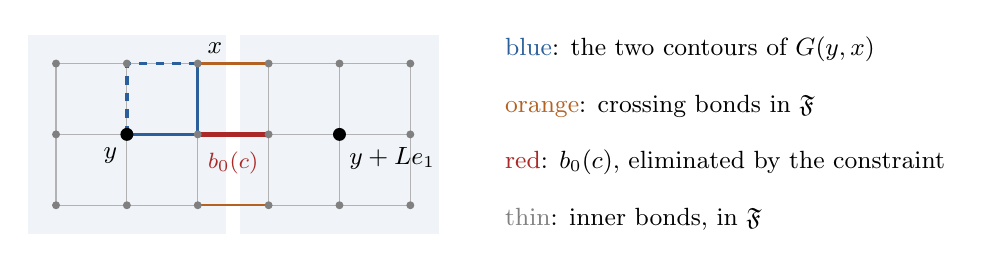
\begin{tikzpicture}[scale=0.9]
\foreach \bx in {0,3} {
  \fill[fblue!7] (\bx-1.4,-1.4) rectangle (\bx+1.4,1.4);
  \foreach \i in {-1,0,1} \foreach \j in {-1,0} \draw[gray!60] (\bx+\i,\j)--(\bx+\i,\j+1);
  \foreach \i in {-1,0} \foreach \j in {-1,0,1} \draw[gray!60] (\bx+\i,\j)--(\bx+\i+1,\j);
}
\foreach \j in {-1,1} \draw[forange,thick] (1,\j)--(2,\j);
\draw[fred,ultra thick] (1,0)--(2,0);
\draw[fblue,very thick] (0,0)--(1,0)--(1,1);
\draw[fblue,very thick,dashed] (0,0)--(0,1)--(1,1);
\foreach \bx in {0,3} \foreach \i in {-1,0,1} \foreach \j in {-1,0,1} \fill[gray] (\bx+\i,\j) circle (1.6pt);
\fill[black] (0,0) circle (2.6pt);
\fill[black] (3,0) circle (2.6pt);
\node[below left,font=\small] at (0,-0.05) {$y$};
\node[below right,font=\small] at (3,-0.05) {$y+Le_1$};
\node[above right,font=\small] at (1,1) {$x$};
\node[fred,font=\footnotesize] at (1.5,-0.4) {$b_0(c)$};
\node[font=\small,align=left,anchor=west] at (5.2,1.2) {\textcolor{fblue}{blue}: the two contours of $G(y,x)$};
\node[font=\small,align=left,anchor=west] at (5.2,0.4) {\textcolor{forange}{orange}: crossing bonds in $\mathfrak F$};
\node[font=\small,align=left,anchor=west] at (5.2,-0.4) {\textcolor{fred}{red}: $b_0(c)$, eliminated by the constraint};
\node[font=\small,align=left,anchor=west] at (5.2,-1.2) {\textcolor{gray}{thin}: inner bonds, in $\mathfrak F$};
\end{tikzpicture}
\caption{Two centred blocks $B'(y)$, $B'(y+Le_1)$ of $\T$ for $d=2$, $L=3$. The bond $b_0(c)$ is the middle bond of the straight contour $[c]$ from $y$ to $y+Le_1$. The blocks, the crossing bonds and $b_0(c)$ are invariant under the reflections that map the pair of blocks onto itself; the family $G(y,x)$ is mapped onto the family of the image of $x$.}
\label{fig:blocks-sym}
\end{figure}

\subsection{Ba\l aban's exponential gauge fixing}\label{ss:32.2}

The integrand of \eqref{eq:rg-map} is invariant under the group
\[
\mathcal G'=\{u:\T\to G:\ u|_{\T'}=1\}
\]
of Section~\ref{sec:rg-step}, by Lemma~\ref{lem:one-step-basic}(b). Following Ba\l aban \cite[(0.14)--(0.16)]{BalYM4I}, we fix this invariance by exponential weights in the averaged contour variables, not by $\delta$-functions; the latter would define a nonlinear slice. Let
\[
\mathfrak M=\big\{V\ \text{real configuration on }\T:\ |\ell(V(\partial p))|\le\eps_M\ \text{for all plaquettes }p\text{ of }\T\big\},\qquad\eps_M=\frac{r_M}{8L^2},
\]
be a quantitative form of Ba\l aban's set of regular configurations \cite[p.~254]{BalYM4I}; in the units of step $k$, $\mathfrak M=\mathfrak U_k(\eps_M)$. By Lemma~\ref{lem:stokes-avg} and Lemma~\ref{lem:one-step-basic}(a), for $V\in\mathfrak M$ all averaged contour variables $V(y,x)$ are defined and real, their families lie in $\cD_{3L^2\eps_M}\subset\cD_{r_M/2}$, and $\mathfrak a'(V)$ is defined and real. The set $\mathfrak M$ is invariant under real gauge transformations of any size and under $\mathfrak S_{k+1}$ (Section~\ref{sec:averaging}). The base lies in it with a margin: by Lemma~\ref{lem:composition}(a), $W\in\mathfrak U_k(2(C_*+1)L^{-2}\eps'_1)$, and $(C_*+1)\eps'_1\le c_1\le r_M/128$ (Lemma~\ref{lem:one-step-regularity}), so
\begin{equation}\label{eq:base-regular}
|\ell(W(\partial p))|\le2(C_*+1)L^{-2}\eps'_1\le\tfrac18\eps_M\qquad\text{for all plaquettes }p.
\end{equation}

\begin{definition}[Gauge fixing relative to the base]\label{def:gauge-fixing}
For $u\in G^c$ put
\[
\phi(u)=\exp\Big(-\frac1{g^2}\Big[\mathsf N-\tfrac12\operatorname{tr}\big(u+u^{-1}\big)\Big]\Big),\qquad z=z(g)=\int_G\phi(u)\,du .
\]
For a real configuration $W_\circ\in\mathfrak M$ and a configuration $V$ whose averaged contour variables are defined, put
\[
\mathrm{gf}_{W_\circ}(V)=\prod_{y\in\T'}\ \prod_{x\in B'(y)\setminus\{y\}}z^{-1}\,\phi\big(V(y,x)\,W_\circ(y,x)^{-1}\big).
\]
In this part $W_\circ=W$ is the base, and we write $\mathrm{gf}_W$.
\end{definition}

For $u\in G$, $\mathsf N-\frac12\operatorname{tr}(u+u^{-1})=\mathsf N-\operatorname{Re}\operatorname{tr}u=\frac12|u-1|^2$, and at $u=e^{\ii H}$ it equals $f(H):=\mathsf N-\operatorname{tr}\cos H=\frac12\operatorname{tr}H^2+O(|H|^4)$. This is the normalization of the plaquette terms of the Wilson action in Section~\ref{sec:action}, and $\operatorname{tr}H^2=|H|^2$ for $H\in\mathfrak g$. The function $\phi$ is a class function, $0<\phi\le1$ on $G$, and $\phi(u)=1$ only for $u=1$. By Laplace's method, $z(g)=\sigma(0)(2\pi g^2)^{\dim\mathfrak g/2}(1+O(g^2))$ as $g\to0$, with $\sigma$ the density of the Haar measure in exponential coordinates (Section~\ref{subsec:exact-formula}). The strength of the gauge fixing is that of the action, as in \cite[(0.19)]{BalYM4I}. For any fixed $a_{\rm gf}>0$ one may replace $g^{-2}$ in the weight by $a_{\rm gf}g^{-2}$ and compute $z$ at that same strength. The normalized Haar-orbit identity is unchanged; the full function $\Phi_W$, its remainder $G_3$, and the quadratic gauge-fixing term are multiplied by $a_{\rm gf}$. The ensuing coercivity and upper-bound constants may depend on this fixed positive strength, and the normalization changes by a background-independent factor. Ba\l aban's weights contain in addition the restriction $\chi(|U(y,x)-1|<\eps_0)$; here the small-field region is defined by the cutoff of Definition~\ref{def:chi-w} instead, on whose support that factor would be $1$.

For a complex field $Z$ on the bonds of $\T$ and $x\in B'(y)$ put
\[
H_{y,x}(Z)=\ell\big((e^{\ii Z}W)(y,x)\,W(y,x)^{-1}\big),
\]
whenever the averaged contour variable is defined and $|(e^{\ii Z}W)(y,x)\,W(y,x)^{-1}-1|<1$, the domain of $\ell$ (Section~\ref{ss:21.2}). The proof of Lemma~\ref{lem:exp-gauge}(c) verifies both conditions on its small complex $Z$-ball, by Lemma~\ref{lem:group-average}(a),(e). For complex fields we use the bilinear pairing $\ip AB=\sum_{y\in\T'}\sum_{x\in B'(y)}\operatorname{tr}(A(y,x)B(y,x))$ on functions of the pairs $(y,x)$; for real fields $\ip AA=\|A\|^2$. Recall $\mathfrak G_WZ(y,x)=\lambda_W(y,x)[Z]$ from Definition~\ref{def:avg-transport}, in the units of step $k$.

\begin{lemma}[Exponential gauge fixing]\label{lem:exp-gauge}
Let $W_\circ\in\mathfrak M$ be real.
\begin{enumerate}[label=(\alph*)]
\item \emph{(Faddeev--Popov identity.)} Let $f$ be an integrable function of real configurations on $\T$ with $f(V^u)=f(V)$ for all $u\in\mathcal G'$, and $f=0$ outside $\mathfrak M$. Then
\[
\int\prod_bdV(b)\ f(V)=\int\prod_bdV(b)\ \mathrm{gf}_{W_\circ}(V)\,f(V).
\]
\item \emph{(Invariance.)} For $V\in\mathfrak M$ and every real gauge transformation $u$ on $\T$, of any size, $\mathrm{gf}_{W_\circ^u}(V^u)=\mathrm{gf}_{W_\circ}(V)$. For $r\in\mathfrak S_{k+1}$, $\mathrm{gf}_{rW_\circ}(rV)=\mathrm{gf}_{W_\circ}(V)$.
\item \emph{(Expansion.)} For $V\in\mathfrak M$, $0<\mathrm{gf}_{W_\circ}(V)\le z^{-|\T\setminus\T'|}$, with equality if and only if $V(y,x)=W_\circ(y,x)$ for all $y\in\T'$, $x\in B'(y)$. There is $c_0>0$, depending only on $G$, such that for complex $Z$ with $|Z|_\infty\le c_0L^{-1}$ the averaged contour variables of $e^{\ii Z}W_\circ$ are defined, and
\[
\mathrm{gf}_{W_\circ}(e^{\ii Z}W_\circ)=z^{-|\T\setminus\T'|}e^{-g^{-2}\Phi_{W_\circ}(Z)},
\]
\[
\Phi_{W_\circ}(Z)=\sum_{y\in\T'}\sum_{x\in B'(y)}f\big(H_{y,x}(Z)\big)=\tfrac12\ip{\mathfrak G_{W_\circ}Z}{\mathfrak G_{W_\circ}Z}+G_3(Z),
\]
with $H_{y,x}$ computed at $W_\circ$. Here $G_3=\sum_{y\in\T'}G_{3,y}$, where $G_{3,y}$ depends only on $Z$ on the inner bonds of $B'(y)$, is holomorphic, real for real $Z$, vanishes to third order at $Z=0$, and satisfies $|G_{3,y}(Z)|\le C_L\max_b|Z(b)|^3$ for $|Z|_\infty\le\frac12c_0L^{-1}$, the maximum over the bonds of $B'(y)$. In particular $\Phi_{W_\circ}$ depends only on $Z$ on inner bonds, and $|G_3(Z)|\le C_L|Z|_\infty\|Z\|^2$.
\end{enumerate}
\end{lemma}

\begin{proof}\hasdetail{lem:exp-gauge}
(a) For real $u$ of any size and $V\in\mathfrak M$, \eqref{eq:avg-contour-gauge} gives $V^u(y,x)=u(y)V(y,x)u(x)^{-1}$. For $u\in\mathcal G'$ this is $V(y,x)u(x)^{-1}$, since $u(y)=1$. Fix $V\in\mathfrak M$. Each $x\in\T\setminus\T'$ lies in exactly one block $B'(y)$, and is not its centre. The map $u\mapsto V(y,x)u^{-1}W_\circ(y,x)^{-1}$ preserves the normalized Haar measure. Hence, with $du=\prod_{x\in\T\setminus\T'}du(x)$,
\[
\int_{\mathcal G'}\mathrm{gf}_{W_\circ}(V^u)\,du=\prod_{y\in\T'}\prod_{x\in B'(y)\setminus\{y\}}z^{-1}\int_G\phi\big(V(y,x)u(x)^{-1}W_\circ(y,x)^{-1}\big)\,du(x)=1 .
\]
Put $\mathrm{gf}_{W_\circ}=0$ outside $\mathfrak M$. Since $\mathfrak M$ is $\mathcal G'$-invariant, $\mathrm{gf}_{W_\circ}(V^u)f(V^u)=0$ for $V\notin\mathfrak M$. The map $V\mapsto V^u$ acts on each bond by a left and a right translation, so it preserves $\prod_bdV(b)$. Since $0\le\mathrm{gf}_{W_\circ}\le z^{-|\T\setminus\T'|}$ and $f$ is integrable, Fubini's theorem applies:
\[
\int dV\,\mathrm{gf}_{W_\circ}f=\int_{\mathcal G'}du\int dV\,\mathrm{gf}_{W_\circ}(V^u)f(V^u)=\int dV\,f(V)\int_{\mathcal G'}\mathrm{gf}_{W_\circ}(V^u)\,du=\int dV\,f(V).
\]
No Faddeev--Popov determinant appears, since the $\mathcal G'$-orbits are integrated with the Haar measure.

(b) By \eqref{eq:avg-contour-gauge}, $V^u(y,x)W_\circ^u(y,x)^{-1}=u(y)\big(V(y,x)W_\circ(y,x)^{-1}\big)u(y)^{-1}$, and $\phi$ is a class function. For $r\in\mathfrak S_{k+1}$, $(rV)(y,x)=V(r^{-1}y,r^{-1}x)$ (Section~\ref{sec:averaging}), and $r$ maps the set of pairs $(y,x)$ with $y\in\T'$, $x\in B'(y)\setminus\{y\}$ bijectively onto itself, since it maps $\T'$ onto $\T'$ and $B'(y)$ onto $B'(ry)$.

(c) The first statement follows from $\phi=e^{-|u-1|^2/2g^2}$ on $G$. Let $\mathbf U=\{W_\circ(\Gamma)\}_{\Gamma\in G(y,x)}$, which lies in $\cD_{r_M/2}$. For $\Gamma\in G(y,x)$ write $(e^{\ii Z}W_\circ)(\Gamma)=e^{\ii\xi_\Gamma}W_\circ(\Gamma)$, where $e^{\ii\xi_\Gamma}=(e^{\ii Z})_{W_\circ}(\Gamma)$ is a product of at most $2(L-1)$ factors $e^{\ii R(W_\circ(\cdot))Z(b)}$ with unitary $R(W_\circ(\cdot))$. By Lemma~\ref{lem:log-estimates}(c), $\xi_\Gamma$ is holomorphic in $Z$ with $|\xi_\Gamma|\le4L|Z|_\infty\le r_M/16$, if $c_0$ is small. By Lemma~\ref{lem:group-average}(a),(e) (and its proof), the family $\{e^{\ii\xi_\Gamma}W_\circ(\Gamma)\}$ lies in $\cD_{r_M}$, the averaged contour variable $(e^{\ii Z}W_\circ)(y,x)=\Av(\{e^{\ii\xi_\Gamma}W_\circ(\Gamma)\})$ is defined and holomorphic in $Z$, and
\[
|H_{y,x}(Z)|=\big|\ell\big(\Av(\{e^{\ii\xi_\Gamma}W_\circ(\Gamma)\})\Av(\mathbf U)^{-1}\big)\big|\le C_M\max_\Gamma|\xi_\Gamma|\le4C_ML|Z|_\infty .
\]
For $c_0$ small this is at most $1$. Since $e^{\ii\ell(h)}=h$, we have $V(y,x)W_\circ(y,x)^{-1}=e^{\ii H_{y,x}(Z)}$ for $V=e^{\ii Z}W_\circ$, and $\phi(e^{\ii H})=e^{-g^{-2}f(H)}$. This gives the formula with $\Phi_{W_\circ}=\sum f(H_{y,x})$. The function $H_{y,x}$ depends only on $Z$ on the bonds of the box spanned by $y$ and $x$, which are inner bonds of $B'(y)$. By Lemma~\ref{lem:avg-transport}(a), $H_{y,x}(sZ)=s\,\mathfrak G_{W_\circ}Z(y,x)+O(s^2)$. Since $f(H)=\frac12\operatorname{tr}H^2+O(|H|^4)$, the second-order part of $\Phi_{W_\circ}$ is $\frac12\ip{\mathfrak G_{W_\circ}Z}{\mathfrak G_{W_\circ}Z}$, and
\[
G_{3,y}(Z)=\sum_{x\in B'(y)}\Big[f\big(H_{y,x}(Z)\big)-\tfrac12\operatorname{tr}\big((\mathfrak G_{W_\circ}Z(y,x))^2\big)\Big]
\]
vanishes to third order. Reality follows from that of $H_{y,x}$ for real $Z$. For the bound let $m$ be the maximum of $|Z(b)|$ over the bonds of $B'(y)$, and $t\mapsto G_{3,y}(tZ)$ for $|t|\le R:=c_0/(Lm)$. There $|H_{y,x}|\le4C_Mc_0\le1$ and $|\mathfrak G_{W_\circ}(tZ)(y,x)|\le C$ (Lemma~\ref{lem:avg-transport}(c)), so $|G_{3,y}(tZ)|\le CL^d$. The maximum principle for $G_{3,y}(tZ)/t^3$ gives $|G_{3,y}(Z)|\le CL^dR^{-3}=CL^{d+3}c_0^{-3}m^3$. Finally $m^3\le|Z|_\infty\sum_{b}|Z(b)|^2$, the sum over the bonds of $B'(y)$, and every bond lies in at most one block.
\end{proof}

Part~(a) is \cite[(0.15)--(0.16)]{BalYM4I}. Ba\l aban's weights are relative to $1$, i.e.\ $W_\circ(y,x)=1$. The real transformation $u\in\mathcal G'$ with $u(x)=W(y,x)$ for $x\in B'(y)$ satisfies $W^u(y,x)=1$, so by~(b) $\mathrm{gf}_W(V)=\mathrm{gf}_{W^u}(V^u)$ is Ba\l aban's weight evaluated at $V^u$. This is the gauge in which Ba\l aban expands the fluctuation integral, with the expansion~(c) of the gauge-fixing term \cite[(2.3)--(2.5)]{BalYM4I}. Relative to the base the gauge fixing needs no gauge condition on $W$, so the local gauges of Parts~VIII--X remain available.

\begin{definition}[Fluctuation cutoff]\label{def:chi-w}
For $w\le\frac12c_G$ and a configuration $V$ on $\T$ put $\chi^{\rm w}(V)=1$ if for every bond $b$ of $\T$ there is $Z(b)\in\mathfrak g$ with $|Z(b)|\le w$ and $V(b)=e^{\ii Z(b)}W(b)$, and $\chi^{\rm w}(V)=0$ otherwise.
\end{definition}

For $w\le\frac12c_G$ the field $Z(b)=\ell(V(b)W(b)^{-1})$ is unique (Lemma~\ref{lem:log-estimates}(a),(d)). The cutoff is a product over all bonds, including the $b_0(c)$; this is Ba\l aban's characteristic function \cite[(2.9)]{BalYM4I}. It depends on $V'$ through $W$. It is not $\mathcal G'$-invariant, but it is covariant: $|\ell(V(b)W(b)^{-1})|$ does not change if $(V,W)$ is replaced by $(V^u,W^u)$ for a real gauge transformation $u$, since then $V(b)W(b)^{-1}$ is conjugated by $u(b_-)$, or by $(rV,rW)$ for $r\in\mathfrak S_{k+1}$, since on reversed bonds $V(-b)W(-b)^{-1}=W(b)^{-1}\big(V(b)W(b)^{-1}\big)^{-1}W(b)$. Let $w\le\frac18\eps_M$. On the support of $\chi^{\rm w}$, write $V(\partial p)$ as a product of four conjugates of the $e^{\pm\ii Z(b)}$ and of $W(\partial p)$, by moving the factors $W(b)$ to the right. By \eqref{eq:base-regular} and Lemma~\ref{lem:log-estimates}(b), every plaquette satisfies $|\ell(V(\partial p))|\le|\ell(W(\partial p))|+4w$. Hence
\begin{equation}\label{eq:chi-w-support}
\operatorname{supp}\chi^{\rm w}\subset\mathfrak U_k\big(2(C_*+1)L^{-2}\eps'_1+4w\big)\subset\mathfrak M\qquad\big(w\le\tfrac18\eps_M\big).
\end{equation}

\subsection{The gauge-fixed step}\label{ss:32.3}

\begin{definition}[Gauge-fixed step]\label{def:gf-step}
For a function $f$ of real configurations on $\T$ that vanishes outside $\mathfrak M$ put
\[
T^{\rm gf}(f)(V')=\int\prod_bdV(b)\ \prod_c\delta\big(\mathfrak a'(V)(c)\,V'(c)^{-1}\big)\ \mathrm{gf}_W(V)\,f(V),
\]
with $W$ the base of $V'$, and the measures and the $\delta$-function of \eqref{eq:rg-map}.
\end{definition}

The integrand may depend on $V'$ through the base $W$ and the reference $U'$; we then write $f=f_{W,U'}$. We call a function $\chi=\chi_{W,U'}$ of configurations $V$ on $\T$, with $0\le\chi\le1$, a \emph{covariant cutoff} if
\begin{enumerate}[label=(C\arabic*)]
\item $\chi_{W^{u|_\T},U'^u}(V^{u|_\T})=\chi_{W,U'}(V)$ for every real gauge transformation $u$ on $\Tf$;
\item $\chi_{rW,rU'}(rV)=\chi_{W,U'}(V)$ for every $r\in\mathfrak S_{k+1}$.
\end{enumerate}
By the paragraph after Definition~\ref{def:chi-w}, $\chi^{\rm w}$ is a covariant cutoff. The identities below between integrals containing $\delta$-functions are first proved with $\delta$ replaced by a continuous class function that is invariant under inversion and concentrated near $1$, for instance a function of $|\ell(u)|$ supported near $1$, and then hold in the limit, as identities of measures. Where $\mathfrak a'$ is a submersion they hold also pointwise for the fibre densities of Section~\ref{sec:rg-step}, at every $V'$ at which the fibre integrals converge absolutely: the substitutions used below are isometries of the bond variables that map fibres of $\mathfrak a'$ onto fibres, and the fibre measure is invariant under $\mathcal G'$. Both invariances are needed: the proofs use $\delta(a^{-1}b)=\delta(ab^{-1})$, and a class function need not be invariant under $u\mapsto u^{-1}$ (for instance on $SU(3)$).

\begin{lemma}[Invariance of the gauge-fixed step]\label{lem:gf-step-invariance}
Let $\rho$ be a gauge-invariant function of real configurations on $\T$, let $\chi$ be a covariant cutoff, and suppose that $\chi\rho$ vanishes outside $\mathfrak M$.
\begin{enumerate}[label=(\roman*)]
\item $T^{\rm gf}(\chi\rho)(V')$ does not depend on the choice of $U'$ in the minimal orbit of $V'$.
\item $T^{\rm gf}(\chi\rho)(V'^{u'})=T^{\rm gf}(\chi\rho)(V')$ for every real gauge transformation $u'$ on $\T'$.
\item For every $r\in\mathfrak S_{k+1}$, $T^{\rm gf}(\chi\cdot r\rho)=r\,T^{\rm gf}(\chi\rho)$, with the actions $(r\rho)(V)=\rho(r^{-1}V)$ and $(rF)(V')=F(r^{-1}V')$ of Section~\ref{sec:rg-step}; that is, $T^{\rm gf}(\chi\cdot r\rho)(rV')=T^{\rm gf}(\chi\rho)(V')$, where on each side $\chi$ is taken at the base and the reference of the argument. In particular, if $\rho(rV)=\rho(V)$ for all $V$, then $T^{\rm gf}(\chi\rho)(rV')=T^{\rm gf}(\chi\rho)(V')$.
\item On the set of the $V'$ as in Lemma~\ref{lem:composition}, $T^{\rm gf}(f)=T(f)$ for every integrable $f$ with $f(V^u)=f(V)$ for $u\in\mathcal G'$ that vanishes outside $\mathfrak M$. Consequently, let $w\le\frac18\eps_M$ and $2(C_*+1)L^{-2}\eps'_1+4w\le\tilde h$, so that $\operatorname{supp}\chi^{\rm w}\subset\mathfrak M\cap\mathfrak U_k(\tilde h)$. Then, on the same set, for every covariant cutoff $\chi$ and every gauge-invariant $\rho\ge0$ on $\mathfrak U_k(\tilde h)$,
\[
T\big(\one_{\mathfrak M\cap\mathfrak U_k(\tilde h)}\rho\big)-T^{\rm gf}(\chi^{\rm w}\chi\rho)=T^{\rm gf}\big((1-\chi^{\rm w}\chi)\one_{\mathfrak M\cap\mathfrak U_k(\tilde h)}\rho\big)\ge0 .
\]
\end{enumerate}
\end{lemma}

\begin{proof}\hasdetail{lem:gf-step-invariance}
The proofs of (i)--(iii) substitute $V=\tilde V^{v}$ or $V=r\tilde V$ in the integral. These substitutions preserve $\prod_bdV(b)$: a gauge transformation acts on each bond by a left and a right translation, and $r$ permutes the bonds, possibly reversing them, which preserves the Haar measure. They also preserve $\mathfrak M$.

(i) Another element of the minimal orbit is $U'^v$ with $v$ real on $\Tf$ and $v|_{\T'}=1$. By Lemma~\ref{lem:one-step-basic}(b), its base is $W^{\tilde v}$ with $\tilde v=v|_\T\in\mathcal G'$. Substitute $V=\tilde V^{\tilde v}$. Then $\mathfrak a'(V)=\mathfrak a'(\tilde V)$, since $\tilde v|_{\T'}=1$. Moreover $\mathrm{gf}_{W^{\tilde v}}(\tilde V^{\tilde v})=\mathrm{gf}_W(\tilde V)$ by Lemma~\ref{lem:exp-gauge}(b), $\chi_{W^{\tilde v},U'^v}(\tilde V^{\tilde v})=\chi_{W,U'}(\tilde V)$ by (C1), and $\rho(\tilde V^{\tilde v})=\rho(\tilde V)$. So the integral with $U'^v$ equals the integral with $U'$.

(ii) Let $u$ be a real gauge transformation on $\Tf$ with $u|_{\T'}=u'$, and $\tilde u=u|_\T$. The configuration $V'^{u'}$ satisfies the hypotheses of Lemma~\ref{lem:composition}, since its curvature is that of $V'$. By Theorem~\ref{thm:variational}(g) and Theorem~\ref{thm:balaban}(a) for the $(k+1)$-step problem, $U'^u$ lies in the minimal orbit of $V'^{u'}$, and by Lemma~\ref{lem:one-step-basic}(b) its base is $W^{\tilde u}$. By (i) we may use this representative. Substitute $V=\tilde V^{\tilde u}$. By Lemma~\ref{lem:one-step-basic}(b),
\[
\mathfrak a'(\tilde V^{\tilde u})(c)\,V'^{u'}(c)^{-1}=u'(c_-)\,\mathfrak a'(\tilde V)(c)V'(c)^{-1}\,u'(c_-)^{-1},
\]
and $\delta$ is a class function. The other factors are invariant as in (i), now with $\tilde u$ in place of $\tilde v$.

(iii) By Proposition~\ref{prop:symmetry}(b) and its proof, $rV'$ satisfies the hypotheses of Lemma~\ref{lem:composition}, and $rU'$ lies in the minimal orbit of $rV'$. Since $\mathfrak S_{k+1}\subset\mathfrak S_k$, Lemma~\ref{lem:one-step-basic} gives $(rU')^{(k)}=rW$. By (i) we may use the reference $rU'$ and the base $rW$ at $rV'$. The hypotheses of the lemma hold with $r\rho$ in place of $\rho$: $r\rho$ is gauge invariant (Proposition~\ref{prop:symmetry}(a)), and $\chi_{rW,rU'}\cdot r\rho=r\big(\chi_{W,U'}\rho\big)$ by (C2), which vanishes outside $r\mathfrak M=\mathfrak M$. Substitute $V=r\tilde V$ in the integral for $T^{\rm gf}(\chi\cdot r\rho)(rV')$. By Lemma~\ref{lem:one-step-basic}(d), $\mathfrak a'(r\tilde V)(c)=\mathfrak a'(\tilde V)(r^{-1}c)$, and $(rV')(c)=V'(r^{-1}c)$. As $c$ runs over the positively oriented bonds of $\T'$, $r^{-1}c$ runs over all bonds of $\T'$, each once up to orientation. If $r^{-1}c=-c''$, then $\mathfrak a'(\tilde V)(-c'')V'(-c'')^{-1}=\mathfrak a'(\tilde V)(c'')^{-1}V'(c'')$ by Lemma~\ref{lem:reversal}, and $\delta(a^{-1}b)=\delta(ab^{-1})$, since $\delta$ is invariant under inversion and conjugation. So the product of the $\delta$-functions is unchanged. Moreover $\mathrm{gf}_{rW}(r\tilde V)=\mathrm{gf}_W(\tilde V)$ by Lemma~\ref{lem:exp-gauge}(b), $\chi_{rW,rU'}(r\tilde V)=\chi_{W,U'}(\tilde V)$ by (C2), and $(r\rho)(r\tilde V)=\rho(\tilde V)$. So the integral equals $T^{\rm gf}(\chi\rho)(V')$. If $\rho\circ r=\rho$, then $r\rho=\rho$, which gives the last claim.

(iv) Let $\varphi$ be a bounded Borel function of configurations on $\T'$ that vanishes outside the set of the $V'$ as in Lemma~\ref{lem:composition}. The function $V\mapsto\varphi(\mathfrak a'(V))f(V)$ is integrable, $\mathcal G'$-invariant by Lemma~\ref{lem:one-step-basic}(b), and vanishes outside $\mathfrak M$. The base $W$, taken at $V'=\mathfrak a'(V)$, is constant on $\mathcal G'$-orbits, and in the proof of Lemma~\ref{lem:exp-gauge}(a) the orbit integral of $\mathrm{gf}_{W_\circ}$ equals $1$ for every $W_\circ$. So that proof, with $W_\circ$ the base on each orbit, gives $\int\prod_bdV(b)\,\varphi(\mathfrak a'(V))\,\mathrm{gf}_W(V)f(V)=\int\prod_bdV(b)\,\varphi(\mathfrak a'(V))f(V)$, that is, $T^{\rm gf}(f)=T(f)$ as measures on that set. If $\mathfrak a'$ is a submersion near the support of $f$ and the fibre integral of $|f|$ at $V'$ is finite, the same argument, run on the fibre, whose measure is $\mathcal G'$-invariant, gives the identity of the fibre densities at $V'$. The inclusion $\operatorname{supp}\chi^{\rm w}\subset\mathfrak M\cap\mathfrak U_k(\tilde h)$ is \eqref{eq:chi-w-support}. The function $\one_{\mathfrak M\cap\mathfrak U_k(\tilde h)}\rho$ is $\mathcal G'$-invariant, since $\mathfrak M$ and $\mathfrak U_k(\tilde h)$ are invariant under real gauge transformations. So $T(\one_{\mathfrak M\cap\mathfrak U_k(\tilde h)}\rho)=T^{\rm gf}(\one_{\mathfrak M\cap\mathfrak U_k(\tilde h)}\rho)$. By the inclusion, $\chi^{\rm w}\chi\rho=\chi^{\rm w}\chi\one_{\mathfrak M\cap\mathfrak U_k(\tilde h)}\rho$. Subtracting gives the identity. The right side is nonnegative, since $\delta\ge0$, $\mathrm{gf}_W\ge0$, $0\le\chi^{\rm w}\chi\le1$ and $\rho\ge0$.
\end{proof}

Lemma~\ref{lem:gf-step-invariance} describes the \emph{modified model}. The small-field step is $T^{\rm gf}(\chi^{\rm w}\chi_\xi\rho)$, with a white-noise cutoff $\chi_\xi$ (Section~\ref{sec:cluster}). The cutoffs act on gauge-fixed variables, so this is not of the form $T(\chi\rho)$ with a $\mathcal G'$-invariant $\chi$. Parts~(i)--(iii) show that it is nevertheless a renormalization group map on gauge-invariant densities that commutes with the lattice symmetries: $T^{\rm gf}(\chi^{\rm w}\chi_\xi\cdot r\rho)=r\,T^{\rm gf}(\chi^{\rm w}\chi_\xi\rho)$ for $r\in\mathfrak S_{k+1}$, by~(iii), since $\chi^{\rm w}\chi_\xi$ is a covariant cutoff (see below). Part~(iv) shows that the discarded part, the difference between the step without cutoffs and the small-field step, is nonnegative. In Section~\ref{sec:cluster} the white-noise cutoff is taken bondwise on $\mathfrak F$ in the coordinates of this section:
\[
\chi_\xi(V)=\prod_{b\in\mathfrak F}\one\big(|\xi_V(b)|\le p_0\big),\qquad\xi_V=g^{-1}C_k^{-1/2}Z_V,\quad Z_V(b)=\ell\big(V(b)W(b)^{-1}\big),\ b\in\mathfrak F,
\]
for $V$ in the support of $\chi^{\rm w}$, with $C_k=C_k(W,U')$ the covariance of Corollary~\ref{cor:covariance}. By Corollary~\ref{cor:covariance}(a),(b), $\xi_{V^{\tilde u}}=R(\tilde u)\xi_V$ and $\xi_{rV}=r_W\xi_V$, with the data transformed accordingly, so $\chi^{\rm w}\chi_\xi$ is a covariant cutoff.

\subsection{Elimination of the constraint}\label{ss:32.4}

For a complex field $Z$ on the bonds of $\T$ and a bond $c$ of $\T'$ put
\[
\ell_c(Z)=\ell\big(\overline X(c)\big),\qquad\overline X=\mathfrak a'(e^{\ii Z}W)\,W'^{-1},
\]
and let $l^{\rm pl}$ be its linearization, $(l^{\rm pl}Z)(c)=\frac{d}{ds}\big|_{s=0}\ell_c(sZ)$; ``pl'' refers to the plain average \eqref{eq:one-step}. The constraint in \eqref{eq:rg-map} is $\ell_c(Z)=0$ for all $c$. Let $\mathsf a:=2(C_*+1)\eps'_1$. By Lemma~\ref{lem:composition} and Proposition~\ref{prop:sharp-curvature}, it bounds the curvature both of $W$ and of the fine reference $U'$, in the units of step $k+1$. The former is what Lemma~\ref{lem:one-step-expansion} needs: by the paragraph after its proof, it applies with $a=\mathsf a$ and $W_{j-1}=W$, which is real and lies in $\mathfrak U_k(\mathsf a)\subset\mathfrak U_k(2\mathsf a)$. In the units of step $k+1$ we write $p'=p_{k+1}=l_{k+1}-\delta_{k+1}D_{W'}\gamma_{k+1}$ for the operator of Lemma~\ref{lem:one-step-expansion}(f) at the reference $U'$, and $q'=q_{k+1}$, $r'=r_{k+1}$, $\gamma'_{\rm lin}=\gamma_{k+1}$.

\begin{lemma}[Local elimination]\label{lem:eliminate}
There are $C,c>0$, depending only on $d$ and $G$, such that the following holds with $\rho_L=cL^{-d-1}$ and $r_L=c^2L^{-2d-1}$, provided $L^{d}\mathsf a\le c$. Moreover $r_L\le\frac18\eps_M$.
\begin{enumerate}[label=(\alph*)]
\item $\ell_c$ is analytic for complex $Z$ with $|Z|\le cL^{-1}$ on the bonds with both endpoints in $B'(c_-)\cup B'(c_+)$, and depends only on these values. Among the bonds $b_0(c')$ it depends only on $Z(b_0(c))$. Moreover $l^{\rm pl}=Lp'$, and $\ell_c(Z)=(l^{\rm pl}Z)(c)+O(L^2|Z|^2)$.
\item $\partial\ell_c/\partial Z(b_0(c))=L^{1-d}R\big(W([c_-,b_0(c)_-])\big)\big(1+\mathfrak r_c(Z)\big)$ with $|\mathfrak r_c(Z)|\le C(L^d\mathsf a+L^{d+1}|Z|)$.
\item For complex $Z$ on $\mathfrak F$ with $|Z|\le r_L$ there is exactly one $\zeta_c(Z)$ with $|\zeta_c(Z)|\le\rho_L$ such that $\ell_c=0$ when $Z(b_0(c))=\zeta_c(Z)$. It is analytic, real for real $Z$, depends only on $Z$ on the bonds of (a), and satisfies $|\zeta_c(Z)|\le CL^d\max|Z|$, the maximum running over those bonds.
\item Let $\hat Z(Z)$ be the field equal to $Z$ on $\mathfrak F$ and to $\zeta_c(Z)$ on $b_0(c)$, and write $\hat Z=\hat Z^1Z+\hat Z^2(Z)+\hat Z^{\ge3}(Z)$ (Taylor expansion). Then $\hat Z^1$ is a linear bijection from fields on $\mathfrak F$ onto
\[
\mathcal Z=\ker l^{\rm pl}=\{B:\ l^{\rm pl}B=0\},
\]
and $\|Z\|\le\|\hat Z^1Z\|\le CL^{d}\|Z\|$. The maps $\hat Z^2$, $\hat Z^{\ge3}$ are supported on the bonds $b_0(c)$ and satisfy $|\hat Z^2(Z)(b_0(c))|\le CL^{3d+1}\max|Z|^2$, the maximum over the bonds of (a).
\end{enumerate}
\end{lemma}

\begin{proof}\hasdetail{lem:eliminate}
(a), (b) We apply Lemma~\ref{lem:one-step-expansion}(f) in the units of step $k+1$, with $a=\mathsf a\le c_2$; its constants $c_2$ and $C$ depend only on $d$ and $G$. There $\delta_k=L^{-1}$, $\delta_{k+1}=1$, and $e^{\ii Z}=e^{\ii\delta_kB}$ with $B=LZ$, so
\[
\ell_c(Z)=(p'B)(c)+c^p_{k+1}(B)(c)=L(p'Z)(c)+c^p_{k+1}(LZ)(c),
\]
for $|B|\le c_2$, i.e.\ $|Z|\le c_2L^{-1}$, with the bounds of Lemma~\ref{lem:one-step-expansion}(c) for $c^p_{k+1}$. This gives $l^{\rm pl}=Lp'$, the expansion, the analyticity and the locality. A bond $b_0(c')$ has both endpoints in $B'(c_-)\cup B'(c_+)$ only if $c'=\pm c$.

Next consider the coefficient of $Z(b_0(c))$ in $L(p'Z)(c)$. By Lemma~\ref{lem:one-step-expansion}(f), $\gamma'_{\rm lin}Z(c_\pm)$ does not depend on $Z(b_0(c))$, and the coefficient of $Z(b_0(c))$ in $(q'Z)(c)$ is $L^{-d}R(W([c_-,b_0(c)_-]))$. The reason is that $[x,x(c)]$ contains $b_0(c)$ only for the $L$ points $x$ on the axis of $c$, for which $G(c_-,x)$ consists of the straight contour $[c_-,x]$. So the coefficient in $L(q'Z)(c)$ is $L^{1-d}R(W([c_-,b_0(c)_-]))$. The bound on $r'$ in Lemma~\ref{lem:one-step-expansion}(b) and the Lipschitz bound for $c^p_{k+1}$ in~(c), applied to $B=LZ$, change it by at most $CL\mathsf a+CL^2|Z|$, i.e.\ relatively by $C(L^d\mathsf a+L^{d+1}|Z|)$. The factor $L^{d+1}$ is genuine. The coefficient $L^{1-d}$ is what remains after a cancellation of terms of order one: the $L$ averaged loops through points of the axis are identically $1$, each of the other $L^d-L$ loops contributes $-L^{-d}$ through $Y([c])^{-1}$, and the outer factor $Y([c])$ contributes $+1$. The non-abelian corrections act on these terms of order one.

(c) Put $M_c=L^{1-d}R(W([c_-,b_0(c)_-]))$ and consider $\Phi(z)=z-M_c^{-1}\ell_c(Z,z)$, where $z$ is the value on $b_0(c)$. By (b), $|\Phi'(z)|\le\frac12$ on $|z|\le\rho_L$ if $c$ is small, since there $L^{d+1}|z|\le c$. By (a), $|\ell_c(Z,0)|\le CL\max|Z|$, since $|p'Z|\le C\max|Z|$ by Lemma~\ref{lem:one-step-expansion}(b). So $|\Phi(0)|\le C_0L^d\max|Z|$, with $C_0$ depending only on $d$ and $G$. For $|Z|\le r_L=c^2L^{-2d-1}$ this is at most $C_0c\,\rho_L\le\frac12\rho_L$ for $c\le1/(2C_0)$. (With the same constant $c$ in $\rho_L$ and $r_L$ the contraction would not close.) So $\Phi$ is a contraction of $\{|z|\le\rho_L\}$ into itself, and its fixed point is the unique zero there. Analyticity follows as in Lemma~\ref{lem:linearizing}. Reality follows from uniqueness, since $\overline X\in G$ for real $Z$. Finally, for $c\le r_M/64$ we have $r_L\le cL^{-2}\le r_M/(64L^2)=\frac18\eps_M$.

(d) Differentiating $\ell_c(\hat Z(Z))=0$ at $Z=0$ gives $(l^{\rm pl}\hat Z^1Z)(c)=0$ for all $c$, so $\hat Z^1Z\in\mathcal Z$. Conversely, $B\in\mathcal Z$ is determined by its values on $\mathfrak F$: by (a), $(l^{\rm pl}B)(c)$ involves among the bonds $b_0(\cdot)$ only $b_0(c)$, with the invertible coefficient of (b) at $Z=0$, so the equation $(l^{\rm pl}B)(c)=0$ fixes $B(b_0(c))$. This gives the bijection. The bound on $\hat Z^1$ follows from $|\zeta^{1}_c(Z)|^2\le CL^{2d}\max|Z|^2\le CL^{2d}\sum|Z(b)|^2$, the sum over the bonds of (a), since each bond lies in a bounded number of these sets. The bound on $\hat Z^2$ follows from Cauchy's estimate, since $|\zeta_c|\le\rho_L$ on $|Z|\le r_L$.
\end{proof}

At the trivial base $W=1$ (and $U'=1$) the averaged contour variables linearize to the means of the line integrals (Lemma~\ref{lem:avg-transport}(b)), and $l^{\rm pl}$ becomes
\begin{equation}\label{eq:q-plain}
(q^{\rm pl}B)(c)=L^{-d}\sum_{x\in B'(c_-)}\Big(\mathfrak G_1B(c_-,x)+B([x,x(c)])-\mathfrak G_1B(c_+,x(c))\Big),
\end{equation}
where $B([x,x(c)])$ is the sum of $B$ over the $L$ bonds of the straight segment. This follows by linearizing \eqref{eq:one-step} at $Y=1$ with Lemma~\ref{lem:group-average}(c), since $L^{-d}\sum_xB([c])=B([c])$ cancels against the outer factor. Equivalently $q^{\rm pl}=L(q-D'\tilde\gamma)$ in the units of step $k+1$, with $q$ the centred tube average, $\tilde\gamma B(y)=L^{-d-1}\sum_{x\in B'(y)}\mathfrak G_1B(y,x)$ and $D'\lambda(c)=\lambda(c_+)-\lambda(c_-)$ (Lemma~\ref{lem:one-step-expansion}(f) and the remark after it). The coefficient of $B(b_0(c))$ in $(q^{\rm pl}B)(c)$ is $L^{1-d}$.

\subsection{The exact formula}\label{subsec:exact-formula}

Let $\sigma$ be the density of the normalized Haar measure in exponential coordinates: $d(e^{\ii Z})=\sigma(Z)\,dZ$ for $|Z|<c_G$, where $dZ$ is the Lebesgue measure on $\mathfrak g$ given by the trace form. It is analytic, positive and $\operatorname{Ad}$-invariant near $0$, and $\sigma(Z)/\sigma(0)=\det\big(\sinh(\tfrac{\ii}{2}\operatorname{ad}Z)/(\tfrac{\ii}{2}\operatorname{ad}Z)\big)=1+O(|Z|^2)$. The $\delta$-function of $G$ is then $\delta(e^{\ii w})=\delta(w)/\sigma(w)$ near $1$.

\begin{proposition}[One step in fluctuation coordinates]\label{prop:exact-step}
Let $V'$ be as in Lemma~\ref{lem:composition}, with $L^d\mathsf a\le c$, and let $w\le r_L$ (so $w\le\rho_L$ and $w\le\frac18\eps_M$). Let $\rho$ be a function of real configurations on $\T$, measurable and bounded on the support of $\chi^{\rm w}$. Then $\chi^{\rm w}\rho$ vanishes outside $\mathfrak M$, which lies in the interior of $\operatorname{dom}\mathfrak a'$, $\mathfrak a'$ is a submersion at every point where $\chi^{\rm w}=1$, and the density of $T^{\rm gf}(\chi^{\rm w}\rho)$ at $V'$, defined in Section~\ref{sec:rg-step}, is
\[
T^{\rm gf}(\chi^{\rm w}\rho)(V')=z^{-|\T\setminus\T'|}\int_{(\mathfrak g)^{\mathfrak F}}\prod_{b\in\mathfrak F}\sigma(Z(b))\,dZ(b)\ \ \chi^{\rm w}\big(\hat Z(Z)\big)\prod_c\mathsf J_c(Z)\ e^{-g^{-2}\Phi_W(Z)}\,\rho\big(e^{\ii\hat Z(Z)}W\big),
\]
where $\chi^{\rm w}(\hat Z)=\prod_b\one(|\hat Z(b)|\le w)$, $\Phi_W$ is the function of Lemma~\ref{lem:exp-gauge}(c), and
\[
\mathsf J_c(Z)=\frac{\sigma(\zeta_c(Z))}{\sigma(0)\,\det\partial\ell_c/\partial Z(b_0(c))}\,,
\]
evaluated at $Z(b_0(c))=\zeta_c(Z)$. For real $Z$ this determinant is positive (see the proof), so it equals its absolute value, which is what the change of variables produces. The integrand is defined to be $0$ if $|Z(b)|>w$ for some $b\in\mathfrak F$. On the remaining set $|Z|_\infty\le w\le r_L\le c_0L^{-1}$, so $\zeta_c(Z)$, $\hat Z(Z)$, $\mathsf J_c(Z)$, $\Phi_W(Z)$ and $\sigma(Z(b))$ are defined, and the factor $\chi^{\rm w}(\hat Z(Z))$ imposes the cutoff also on the bonds $b_0(c)$. The same convention is used for all integrals over fields on $\mathfrak F$ below. Each $\mathsf J_c$ is an analytic function of $Z$ on the bonds of Lemma~\ref{lem:eliminate}(a), and $\mathsf J_c(Z)=L^{(d-1)\dim\mathfrak g}\big(1+O(L^d\mathsf a+L^{2d+1}|Z|_\infty)\big)$, with $|Z|_\infty$ the sup over $\mathfrak F$. The value on $b_0(c)$ is $\zeta_c$, with $|\zeta_c|\le CL^d|Z|_\infty$.
\end{proposition}

\begin{proof}\hasdetail{prop:exact-step}
By \eqref{eq:chi-w-support}, $\chi^{\rm w}$ vanishes outside $\mathfrak M=\mathfrak U_k(\eps_M)$, and $8\eps_ML^2=r_M$, so $\mathfrak M$ lies in the interior of $\operatorname{dom}\mathfrak a'$ (Section~\ref{sec:rg-step}). On its support $V=e^{\ii Z}W$ with $Z(b)\in\mathfrak g$, $|Z(b)|\le w$ on all bonds, and $dV(b)=\sigma(Z(b))dZ(b)$.

\emph{Submersion.} By Lemma~\ref{lem:eliminate}(a),(b), at such $V$ the derivative of $Z\mapsto(\ell_c(Z))_c$ with respect to the variables $Z(b_0(c))$ is block diagonal, with the invertible blocks $L^{1-d}R(W([c_-,b_0(c)_-]))(1+\mathfrak r_c)$; here $|\mathfrak r_c|\le\frac12$, as in the proof of Lemma~\ref{lem:eliminate}(c), since $|Z|\le w\le\rho_L$. Since $\ell_c(Z)=\ell\big(\mathfrak a'(e^{\ii Z}W)(c)\,V'(c)^{-1}\big)$, and the exponential and the logarithm are local diffeomorphisms, $\mathfrak a'$ is a submersion at $V$. So the density at $V'$ is an integral over the fibre $\{\mathfrak a'(V)=V'\}$ (Section~\ref{sec:rg-step}), which we compute with $\delta$-functions. The elimination of $Z(b_0(c))$ below is the change of variables $z\mapsto\ell_c(Z,z)$ in this integral, at fixed variables on $\mathfrak F$.

\emph{The formula.} Since $w\le r_L\le c_0L^{-1}$ for $c$ small, Lemma~\ref{lem:exp-gauge}(c) gives $\mathrm{gf}_W(V)=z^{-|\T\setminus\T'|}e^{-g^{-2}\Phi_W(Z)}$. Moreover $\mathfrak a'(V)(c)V'(c)^{-1}=\overline X(c)=e^{\ii\ell_c(Z)}$. By Lemma~\ref{lem:eliminate}(a), the $\delta$-function for $c$ involves, among the variables $Z(b_0(\cdot))$, only $Z(b_0(c))$. The function $\Phi_W$ involves none of them, since it depends only on inner bonds (Lemma~\ref{lem:exp-gauge}(c)). So the integrals over these variables factorize. For fixed variables on $\mathfrak F$, $Z(b_0(c))\mapsto\ell_c$ has at most one zero in $|Z(b_0(c))|\le w$, by Lemma~\ref{lem:eliminate}(c). It is $\zeta_c(Z)$ if $|\zeta_c(Z)|\le w$; otherwise the integrand vanishes, which is accounted for by the factor $\chi^{\rm w}(\hat Z(Z))$. Hence
\[
\int\sigma(z)\,dz\ \delta\big(e^{\ii\ell_c(Z,z)}\big)\,(\cdots)=\int\sigma(z)\frac{\delta(\ell_c(Z,z))}{\sigma(\ell_c(Z,z))}(\cdots)\,dz=\frac{\sigma(\zeta_c)}{\sigma(0)\,|\det\partial_z\ell_c|}(\cdots)\Big|_{z=\zeta_c} .
\]
\emph{Positivity of the determinant.} By Lemma~\ref{lem:eliminate}(b),
\[
\det\partial_z\ell_c=L^{(1-d)\dim\mathfrak g}\det R\big(W([c_-,b_0(c)_-])\big)\det(1+\mathfrak r_c).
\]
Here $\det R(\cdot)=1$ on $\mathfrak g$, since $G$ is connected (Section~\ref{sec:background}). In the proof of Lemma~\ref{lem:eliminate}(c), $|\mathfrak r_c|\le\frac12$ wherever $\zeta_c$ is defined, so $t\mapsto\det(1+t\mathfrak r_c)$ does not vanish on $[0,1]$, and $\det(1+\mathfrak r_c)>0$ for real $Z$. Hence $|\det\partial_z\ell_c|=\det\partial_z\ell_c$ for real $Z$, and $\mathsf J_c$ is the analytic function of the statement. The bound on $\mathsf J_c$ follows from Lemma~\ref{lem:eliminate}(b),(c), since $L^{d+1}|\zeta_c|\le CL^{2d+1}|Z|_\infty$ and $\sigma(\zeta_c)/\sigma(0)=1+O(|\zeta_c|^2)$.
\end{proof}

No invariance of $\rho$ is used: the gauge fixing has been made by the weight $\mathrm{gf}_W$, and the elimination of the constraint is a change of variables. This is Ba\l aban's representation \cite[(0.16)--(0.19)]{BalYM4I}, \cite[(2.3)--(2.7)]{BalYM4II}: the integration variables are the bonds of $\T$ other than the $b_0(c)$, and the elimination is performed on one bond per coarse bond, so that the Jacobians are local, as in \cite[(17), (20)]{BalUV3}. The representation is exact. No small-field approximation has been made beyond the insertion of $\chi^{\rm w}$, and by Lemma~\ref{lem:gf-step-invariance}(iv) the gauge fixing changes nothing on $\mathcal G'$-invariant integrands supported in $\mathfrak M$.

\section{The coarse effective action}\label{sec:coarse-action}

The integrand of Proposition~\ref{prop:exact-step} depends on the fluctuation in two ways: through the explicit gauge-fixing weight $e^{-g^{-2}\Phi_W}$ of Lemma~\ref{lem:exp-gauge}, and through the action of the background field, $S(U_k(e^{\ii\hat Z}W))$. In this section we study the latter as a function of the coarse configuration. Its gradient is the Lagrange multiplier of the variational problem; its derivatives decay along trees; and its Hessian at the base configuration is comparable with the operator $\boldsymbol\Gamma_\pi-a$ of Part~II. All statements hold for every unit-lattice field $B$ in the stated balls. None of them uses the one-step constraint or a gauge condition on $B$, so they apply to the fields $\hat Z(Z)$ of Section~\ref{sec:fluctuations}, which satisfy the constraint, and to arbitrary fields on all bonds of $\T$ alike.

\paragraph{Setting.} In this section $k\ge1$: the $k$-step operators of Parts~II--V at $U'$ need at least one averaging step (Section~\ref{sec:setup}). The first step, $k=0$, is treated in Section~\ref{subsec:tf-first} (Lemma~\ref{lem:first-step-formula}). Let $W$ be a real configuration on $\T$ in $\mathfrak U_k(\eps_1)$, $\eps_1\le a_1$, and let $U'$ be an element of its minimal orbit. Let $\eps$ be a number such that $U'$ is $(M,\eps)$-regular with $|J_{U'}|\le\eps$; by Theorem~\ref{thm:balaban} one may take $\eps=B_3\eps_1$, and in Section~\ref{sec:fluctuations} we take $\eps=B_3\eps'_1$ (end of Section~\ref{sec:rg-step}). We assume $\eps\le c_6/2$, and we put $r_1:=c_6/4$. In Section~\ref{sec:fluctuations}, $W$ is the base configuration $V^0$ and $U'$ the $(k+1)$-step background. For complex unit-lattice fields $B$ with $|B|_\infty<2r_1$, so that $\eps+|B|_\infty<c_6$, let $A_*(B)$ be the Landau representative relative to $U'$ given by Theorem~\ref{thm:variational}(f), for the coarse configuration $e^{\ii B}W$, and put
\[
\mathcal S(B)=\Phi\big(A_*(B)\big),\qquad\Phi(A)=S(e^{\ii\eta A}U').
\]
The bounds of Proposition~\ref{prop:coarse-action}(c) are stated on the smaller ball $|B|_\infty<r_1$. The margin $r_1$ between the two balls is used only for Cauchy's estimate in the proof of the third-derivative bound. For real $B$, $\mathcal S(B)$ is the minimum of $S$ on $\mathfrak B(e^{\ii B}W)\cap\mathfrak U(\theta_0)$: by Theorem~\ref{thm:variational}(a),(b) the orbit of $\mathsf U(A_*(B))$ is the set of minimizers there, and $S(\mathsf U(A))=\Phi(A)$. If moreover $e^{\ii B}W\in\mathfrak U_k(a_1)$, this orbit is the minimal orbit of Theorem~\ref{thm:balaban}(a), and $\mathcal S(B)=S(U_k(e^{\ii B}W))$; this is the case in all uses below. In particular $\mathcal S$ depends only on the configuration $e^{\ii B}W$, and not on the choice of the reference $U'$.

For bonds $c_1,\dots,c_m$ of $\T$ let $\tau(c_1,\dots,c_m)=\min_{z}\sum_i|c_i-z|$; for $m=2$ this is $|c_1-c_2|$. It satisfies $\tau(c_1,\dots,c_m)\le|c_1-x|+\tau(x,c_2,\dots,c_m)$.

\subsection{Gradient and decay of derivatives}\label{ss:33.1}

\begin{proposition}[The coarse effective action]\label{prop:coarse-action}
There are $C,\gamma_1>0$, independent of $k$, $n$, $\eta$ and $W$, such that:
\begin{enumerate}[label=(\alph*)]
\item $\mathcal S$ is analytic on $\{|B|_\infty<2r_1\}$ and real for real $B$.
\item $\nabla\mathcal S(B)=\omega(B)$, where for real $B$, $\omega(B)$ is the multiplier of Proposition~\ref{prop:euler-lagrange} for the coarse configuration $e^{\ii B}W$; $\omega$ is analytic, and $|\omega(B)|_\infty\le C(\eps+|B|_\infty)$ for $|B|_\infty<2r_1$.
\item For $|B|_\infty<r_1$ and all bonds $c_1,c_2,c_3$:
\[
|\partial_{c_1}\partial_{c_2}\mathcal S(B)|\le Ce^{-\gamma_1|c_1-c_2|},\qquad|\partial_{c_1}\partial_{c_2}\partial_{c_3}\mathcal S(B)|\le Ce^{-\gamma_1\tau(c_1,c_2,c_3)},
\]
where $\partial_c$ is the derivative with respect to $B(c)$, the components being suppressed.
\item Put $\omega_0=\omega(0)$ and $\Delta^0=d^2\mathcal S(0)$. For $|B|_\infty\le r_1/2$,
\[
\mathcal S(B)=\mathcal S(0)+\ip{\omega_0}B+\tfrac12\Delta^0(B,B)+\mathcal S_3(B),\qquad|\mathcal S_3(B)|\le C|B|_\infty\|B\|^2 .
\]
\end{enumerate}
\end{proposition}

\begin{proof}\hasdetail{prop:coarse-action}
(a) $A_*$ is analytic with $|A_*(B)|_{C^1}\le C_6(\eps+|B|_\infty)\le c_5$, and $\Phi$ is analytic there (Proposition~\ref{prop:action}).

(b) For real $B$, Proposition~\ref{prop:euler-lagrange} gives $\nabla\Phi(A_*(B))=d\mathcal Q(A_*(B))^T\omega(B)$. Differentiating the constraint $\ell(\mathcal Q(e^{\ii\eta A_*(B)}))=B$ gives $d\mathcal Q(A_*)\,dA_*(B)=I$. Hence
\[
d\mathcal S(B)h=\ip{\nabla\Phi(A_*)}{dA_*h}=\ip{\omega}{d\mathcal Q(A_*)dA_*h}=\ip\omega h .
\]
Applying $\bH^T$ to the Euler--Lagrange equation gives
\[
\omega(B)=\big((I+d\Cav_k(A_*)\bH)^{-1}\big)^T\bH^T\nabla\Phi(A_*(B)).
\] This expression is analytic in complex $B$ and defines the continuation of $\omega$. The identities $\nabla\Phi(A_*)=d\mathcal Q(A_*)^T\omega$ and $\nabla\mathcal S=\omega$ hold for real $B$, hence for complex $B$ by the identity theorem: the real ball is a totally real submanifold of maximal dimension. The bound for real $B$ is Proposition~\ref{prop:euler-lagrange}; for complex $B$ it follows from the formula, Lemma~\ref{lem:sup-bounds}, Proposition~\ref{prop:action}(a), and the identity $\bH^TD^TDA_*=(\boldsymbol\Gamma_\pi-a)\bQ A_*$. This is the second identity in the proof of Lemma~\ref{lem:V-bounds}; it applies since $RD^TA_*=RD^TA'_*=0$ also for complex $B$ (Lemma~\ref{lem:linearizing}, $A'_*\in\bH B+\cX$). The bound $|A_*|_{C^1}\le C(\eps+|B|_\infty)$ alone would not bound $D^TDA_*$ pointwise.

(c) \emph{Second derivatives.} We prove the bound on the larger ball $|B|_\infty<2r_1$. Let $|B|_\infty<2r_1$. Differentiating $d\mathcal S(B)h=\ip{\nabla\Phi(A_*)}{dA_*h}$ once more,
\[
d^2\mathcal S(B)[h_1,h_2]=d^2\Phi(A_*)[dA_*h_1,dA_*h_2]-\ip{\omega}{d^2\Cav_k(A_*)[dA_*h_1,dA_*h_2]},
\]
where we used $\ip{\nabla\Phi}{d^2A_*[h_1,h_2]}=\ip\omega{d\mathcal Q\,d^2A_*[h_1,h_2]}$ and the second derivative of the constraint, $d\mathcal Q\,d^2A_*[h_1,h_2]+d^2\Cav_k(A_*)[dA_*h_1,dA_*h_2]=0$. Now:
\begin{itemize}
\item $d^2\Phi(A)=D^TD+d^2\mathcal N(A)$, where $d^2\mathcal N(A)$ is a sum of plaquette-local terms with bounded coefficients (proof of Proposition~\ref{prop:action}(c));
\item $d^2\Cav_k(A)[u,v](c)$ is bounded by $C\|u\|_{S_c}\|v\|_{S_c}$, by polarization of Proposition~\ref{prop:Q-expansion}(c);
\item by Theorem~\ref{thm:variational}(f), which holds for complex $B$ with $\eps+|B|_\infty<c_6$, and here $\eps+|B|_\infty<2r_1+2r_1=c_6$: $|dA_*\delta_{c_i}|+|\nabla dA_*\delta_{c_i}|\le Ce^{-\gamma'|x-c_i|}$.
\end{itemize}
Hence $|\partial_{c_1}\partial_{c_2}\mathcal S(B)|\le C\sum_xe^{-\gamma'(|x-c_1|+|x-c_2|)}\eta^d\le Ce^{-\gamma'|c_1-c_2|/2}$ for $|B|_\infty<2r_1$.

\emph{Third derivatives.} Let $|B|_\infty<r_1$, and let $e$ be a unit vector of $\mathfrak g$. For complex $t$ with $|t|<2r_1-|B|_\infty$ we have $|B+te\,\delta_{c_3}|_\infty<2r_1$. Since $2r_1-|B|_\infty>r_1$, the function $t\mapsto\partial_{c_1}\partial_{c_2}\mathcal S(B+te\,\delta_{c_3})$ is analytic on a neighbourhood of the closed disc $|t|\le r_1$, and, by the bound just proved on the larger ball, it is bounded there by $Ce^{-\gamma'|c_1-c_2|/2}$. By Cauchy's estimate on the circle $|t|=r_1$,
\[
|\partial_{c_1}\partial_{c_2}\partial_{c_3}\mathcal S(B)|\le Cr_1^{-1}e^{-\gamma'|c_1-c_2|/2}.
\]
The left side is symmetric in $c_1,c_2,c_3$. So the bound holds with $|c_1-c_2|$ replaced by the largest distance $D$ between two of the three bonds. Taking $z=c_1$ in the definition of $\tau$ gives $\tau(c_1,c_2,c_3)\le|c_2-c_1|+|c_3-c_1|\le2D$. This proves (c) with $\gamma_1=\gamma'/4$. No bound on the second or higher derivatives of $A_*$ on the fine lattice is used.

(d) Fix $B$ and a bond $c$, and let $R(s)=\omega(sB)(c)$ for complex $s$ with $|s|\,|B|_\infty<r_1$. By (c), $|R'(s)|=|d\omega(sB)B(c)|\le C\sum_{c'}e^{-\gamma_1|c-c'|}|B(c')|=:K_c$ on this disc. By the Schwarz lemma applied to $R'(s)-R'(0)$, $|R'(s)-R'(0)|\le4K_c|B|_\infty r_1^{-1}$ for $|s|\le1$, when $|B|_\infty\le r_1/2$. By (b),
\[
\mathcal S_3(B)=\int_0^1\ip{\omega(tB)-\omega_0-t\,d\omega(0)B}B\,dt,\qquad|\mathcal S_3(B)|\le C|B|_\infty\sum_c K_c|B(c)|\le C|B|_\infty\|B\|^2,
\]
by the Schur test.
\end{proof}

Part (b) is the discrete form of the statement that the derivative of the minimal action with respect to the constraint is the Lagrange multiplier. Part (c) is what makes the coarse action, and the Gaussian measure it defines, local.

\subsection{The Hessian at the base configuration}\label{ss:33.2}

Recall that $\bH=\bH(U')$, $\cX=\{A:RD^TA=0,\ \bQ A=0\}$ and $\boldsymbol\Gamma_\pi=\boldsymbol\Gamma_\pi(U')$ are taken at $U'$ with the averaging pair $(Q'_k(U'),\bQ_k(U'))$, and that
\begin{equation}\label{eq:H-effective}
\bH^TD^TD\bH=\boldsymbol\Gamma_\pi-a .
\end{equation}
This follows from the first identity in the proof of Lemma~\ref{lem:V-bounds} and $S\bH=G'RD^T\bH=0$. At $U'=1$ the right-hand side is the operator $\bD$ of Proposition~\ref{prop:eff-action-gauge}.

\begin{proposition}[The Hessian]\label{prop:hessian}
\begin{enumerate}[label=(\alph*)]
\item For real $B$,
\[
\Delta^0(B,B)=\min\big\{q_2(A,A):\ \bQ A=B,\ RD^TA=0\big\},
\]
\[
q_2(A,A)=\|DA\|^2+d^2\mathcal N(0)[A,A]-\ip{\omega_0}{d^2\Cav_k(0)[A,A]},
\]
and the minimum is attained at $A=dA_*(0)B$.
\item $\big|\Delta^0(B,B)-\ip B{(\boldsymbol\Gamma_\pi-a)B}\big|\le C\eps\|B\|^2$.
\item $\Delta^0$ is real symmetric with decay $(C,\gamma_1)$.
\item For every real gauge transformation $u$ on $\Tf$, replacing $(W,U')$ by $(W^{u|_\T},U'^u)$ replaces $\Delta^0$ by $R(u)\Delta^0R(u)^{-1}$ and $\omega_0$ by $R(u)\omega_0$, where $R(u)$ acts on unit-lattice fields by $R(u(b_-))$.
\item For every $r\in\mathfrak S_k$, replacing $(W,U')$ by $(rW,rU')$ replaces $\Delta^0$ by $r_W\Delta^0r_W^{-1}$ and $\omega_0$ by $r_W\omega_0$. Here $(r_WB)(b)=B(r^{-1}b)$, with $B(-b)=-R(W(b))^{-1}B(b)$ on negatively oriented bonds, as in Proposition~\ref{prop:linearized-averages}(g); $r_W$ is orthogonal.
\end{enumerate}
\end{proposition}

\begin{proof}\hasdetail{prop:hessian}
(a) Let $A^1$ satisfy $\bQ A^1=B$ and $RD^TA^1=0$. Put $A(t)=tA^1-\bH\mathcal D(tA^1)$. By Lemma~\ref{lem:linearizing}, $RD^TA(t)=0$ and $\ell(\mathcal Q(e^{\ii\eta A(t)}))=tB$. Moreover $\mathcal D(tA^1)=t^2C^{{\rm av},(2)}_k(A^1)+O(t^3)$, where $C^{{\rm av},(2)}_k(A)=\frac12d^2\Cav_k(0)[A,A]$. For real $t$ near $0$ the configuration $\mathsf U(A(t))$ lies in $\mathfrak B(e^{\ii tB}W)\cap\mathfrak U(\theta_0)$. By Theorem~\ref{thm:variational}(b), $\mathcal S(tB)\le\Phi(A(t))$. Expand $\Phi$ with Proposition~\ref{prop:action}:
\[
\Phi(A(t))=\mathcal S(0)+t\ip J{A^1}+t^2\Big(\tfrac12\|DA^1\|^2+\tfrac12d^2\mathcal N(0)[A^1,A^1]-\ip J{\bH C^{{\rm av},(2)}_k(A^1)}\Big)+O(t^3),
\]
with $J=J_{U'}=\nabla\Phi(0)=\bQ^T\omega_0$. Then $\ip J{A^1}=\ip{\omega_0}B$ and $\ip J{\bH C^{{\rm av},(2)}_k(A^1)}=\ip{\omega_0}{C^{{\rm av},(2)}_k(A^1)}$, since $\bQ\bH=I$. The terms of first order agree with those of $\mathcal S(tB)$. So the inequality for $t\to0$ gives $\Delta^0(B,B)\le q_2(A^1,A^1)$.

For equality, expand $\mathcal S(tB)=\Phi(A_*(tB))$ directly. We have $A_*(tB)=tA^1+t^2A^2+O(t^3)$ with $A^1=dA_*(0)B$, both in the slice, and the constraint gives $\bQ A^1=B$, $\bQ A^2+C^{{\rm av},(2)}_k(A^1)=0$. Hence the coefficient of $t^2$ is $\frac12\|DA^1\|^2+\frac12d^2\mathcal N(0)[A^1,A^1]+\ip J{A^2}$, and $\ip J{A^2}=\ip{\omega_0}{\bQ A^2}=-\ip{\omega_0}{C^{{\rm av},(2)}_k(A^1)}$. So $\Delta^0(B,B)=q_2(A^1,A^1)$.

(b) Write $A=\bH B+h$ with $h\in\cX$. Then $\|DA\|^2=\|D\bH B\|^2+\|Dh\|^2$, since $\ip{Dh}{D\bH B}=0$ for $h\in\cX$, and $\|D\bH B\|^2=\ip B{(\boldsymbol\Gamma_\pi-a)B}$ by \eqref{eq:H-effective}. By Proposition~\ref{prop:action}(c) at $A=0$, $|d^2\mathcal N(0)[A,A]|\le C\eps(\|A\|^2+\|\nabla A\|^2)$. By Proposition~\ref{prop:Q-expansion}(c) and $|\omega_0|\le C\eps$, $|\ip{\omega_0}{d^2\Cav_k(0)[A,A]}|\le C\eps\|A\|^2$. Moreover:
\begin{itemize}
\item $\|\bH B\|+\|\nabla\bH B\|\le C\|B\|$, by the decay of $\bH$ and $D\bH$, the identity $D^T\bH B=P_\cV D^T\bH B$, and Lemma~\ref{lem:weitzenbock};
\item $\|h\|^2+\|\nabla h\|^2\le c_X^{-1}\|Dh\|^2$, by Lemma~\ref{lem:X-coercive}.
\end{itemize}
Hence
\[
\ip B{(\boldsymbol\Gamma_\pi-a)B}-C\eps\|B\|^2+(1-C\eps)\|Dh\|^2\le q_2(A,A).
\]
Taking the minimum over $h$ gives the lower bound; $h=0$ gives the upper bound.

(c) is Proposition~\ref{prop:coarse-action}(c) at $B=0$. (d) follows from the covariance of the variational problem, Theorem~\ref{thm:variational}(g), and $\mathcal S$ depending only on $e^{\ii B}W$: $(e^{\ii B}W)^{u|_\T}=e^{\ii R(u)B}W^{u|_\T}$.

(e) Apply Theorem~\ref{thm:variational}(h) with the reference $U_0=U'$ and $V=W$, so $\beta=0$; its hypotheses hold since $W_k(U')=W$ and $\eps\le c_6/2$. Its first sentence gives that $rU'$ is real and $(M,\eps)$-regular with $|J_{rU'}|\le\eps$, and that $(rU')^{(k)}=rW$. This needs no bound $\eps\le\eps_{\rm B}$. By Theorem~\ref{thm:balaban}(c), $rW\in\mathfrak U_k(\eps_1)$, and the minimal orbit of $rW$ is the image under $r$ of the minimal orbit of $W$; since $U'$ lies in the latter, $rU'$ lies in the former. So the setting applies to $(rW,rU')$, with the same $\eps$. By the convention on reversed bonds, $e^{\ii r_WB}(rW)=r(e^{\ii B}W)$. For real $B$ with $|B|_\infty<r_1$, Theorem~\ref{thm:variational}(h) gives $A_*(r_WB;rU')=r_{U'}A_*(B;U')$, and $\Phi_{rU'}(r_{U'}A)=\Phi_{U'}(A)$ by $e^{\ii\eta\,r_{U'}A}\,rU'=r(e^{\ii\eta A}U')$ and $S\circ r=S$. Hence $\mathcal S_{rW}(r_WB)=\mathcal S_W(B)$ for real $B$, where the index denotes the base, and for complex $B$ by the identity theorem. Differentiating at $B=0$ and using that $r_W$ preserves the pairing gives the claim. Only the coarse action enters. The operators $\boldsymbol\Gamma_\pi$, $\bH$, $\bC$ of Parts~II--III are not covariant under reflections at curved backgrounds (Remark~\ref{rem:symmetry-reflections}), and (e) is not derived from~(b).
\end{proof}

\subsection{Dependence on the base configuration}\label{ss:33.3}

Let $\hat\beta$ be a complex unit-lattice field with $|\hat\beta|_\infty\le r_1/4$, and $\hat W=e^{\ii\hat\beta}W$ (bondwise product). For real $\hat\beta$ we have $\mathcal S_{\hat W}(B)=\mathcal S_W(B\star\hat\beta)$, with $B\star\hat\beta=\ell(e^{\ii B}e^{\ii\hat\beta})$ bondwise. We use this formula as the definition for complex $\hat\beta$. It defines $\mathcal S_{\hat W}$ analytically in $(\hat\beta,B)$ for $|B|_\infty\le r_1/4$, and in particular $\omega_0(\hat W)$ and $\Delta^0(\hat W)$.

\begin{proposition}[Dependence on the base]\label{prop:base-dependence}
$\omega_0(\hat W)$ and $\Delta^0(\hat W)$ are analytic in $\hat\beta$. Their derivatives with respect to $\hat\beta(c)$ satisfy
\[
|\partial_{\hat\beta(c)}\omega_0(\hat W)(c_1)|\le Ce^{-\gamma_1|c-c_1|},\qquad|\partial_{\hat\beta(c)}\Delta^0(\hat W)(c_1,c_2)|\le Ce^{-\gamma_1\tau(c,c_1,c_2)} .
\]
\end{proposition}

\begin{proof}\hasdetail{prop:base-dependence}
$\omega_0(\hat W)=\partial_B\mathcal S_W(B\star\hat\beta)|_{B=0}$ and $\Delta^0(\hat W)=\partial^2_B\mathcal S_W(B\star\hat\beta)|_{B=0}$. The map $(B,\hat\beta)\mapsto B\star\hat\beta$ is bondwise analytic. Its derivatives in $B$ at $B=0$ are bondwise analytic functions of $\hat\beta$. The chain rule expresses the derivatives in terms of $d^m\mathcal S_W(\hat\beta)$, $m\le3$, contracted with bondwise factors. Proposition~\ref{prop:coarse-action}(c) at $B=\hat\beta$, with $|\hat\beta|_\infty\le r_1/4<r_1$, gives the bounds.
\end{proof}

Proposition~\ref{prop:base-dependence} controls the dependence on small changes of the base configuration. Changes that are not small, for example replacing the configuration far away by a different one, require a representation of the operators by terms that depend on the background only locally. This is the random-walk expansion of Section~\ref{sec:random-walk}, which will be developed for the present operators in the next part.

\section{The fluctuation covariance and the step}\label{sec:covariance}

We return to the setting of Section~\ref{sec:fluctuations}: $W=V^0$ is the base configuration of the step, $U'=U_{k+1}(V')$, and $\eps=B_3\eps'_1$. The objects of Section~\ref{sec:coarse-action} are taken at this $W$ and $U'$.

\subsection{The quadratic form of the step}\label{ss:34.1}

\begin{lemma}[Expansion in the variables $\mathfrak F$]\label{lem:step-quadratic}
Let $r_2=\min(cL^{-2d-2},\,cL^{-d}a'_1)$ with $c>0$ small, depending only on $d$, $G$, $L$ and $r_1=c_6/4$ of Proposition~\ref{prop:coarse-action} (the proof needs $2cL^{-2d-2}\le\frac12r_L$, $2cL^{-2d-2}\le\frac12c_0L^{-1}$ with $c_0$ of Lemma~\ref{lem:exp-gauge}(c), $CL^{-d-2}c\le\frac14r_1$ and $Cc\le\frac12$), $a'_1$ as in Lemma~\ref{lem:composition}(c), and assume $4(C_*+1)L^{-2}\eps'_1\le a'_1$. For complex fields $Z$ on $\mathfrak F$ with $|Z|_\infty\le r_2$ put
\[
F(Z)=\mathcal S(\hat Z(Z))+\Phi_W(Z),
\]
with $\Phi_W$ as in Lemma~\ref{lem:exp-gauge}(c). Then $F$ is analytic, $F(Z)=S(U_k(e^{\ii\hat Z(Z)}W))+\Phi_W(Z)$ for real $Z$, and
\[
F(Z)=S(U')+\tfrac12\Delta_k(Z,Z)+\mathcal V(Z)+G_3(Z),
\]
\[
\Delta_k(Z,Z)=\Delta^0(\hat Z^1Z,\hat Z^1Z)+2\ip{\omega_0}{\hat Z^2(Z)}+\|\mathfrak G_WZ\|^2 .
\]
Here $\mathcal V$ is the remainder of the coarse action,
\[
\mathcal S(\hat Z(Z))=S(U')+\tfrac12\Delta^0(\hat Z^1Z,\hat Z^1Z)+\ip{\omega_0}{\hat Z^2(Z)}+\mathcal V(Z),
\]
$G_3$ is the remainder of the gauge fixing (Lemma~\ref{lem:exp-gauge}(c)), and $|\mathcal V(Z)|+|G_3(Z)|\le C_L|Z|_\infty\|Z\|^2$. For complex $Z$, $\|\mathfrak G_WZ\|^2$ stands for the bilinear form $\ip{\mathfrak G_WZ}{\mathfrak G_WZ}$. It involves only inner bonds, so $\|\mathfrak G_WZ\|=\|\mathfrak G_W\hat Z^1Z\|$. In particular $F$ has no linear term.
\end{lemma}

\begin{proof}\hasdetail{lem:step-quadratic}
By Lemma~\ref{lem:eliminate}, $\hat Z$ is analytic on $|Z|_\infty\le2r_2\le r_L$ with $|\hat Z(Z)|_\infty\le CL^d|Z|_\infty\le r_1/2$, so $\mathcal S\circ\hat Z$ is analytic on the disc of radius $2r_2$ by Proposition~\ref{prop:coarse-action}(a). Since $2r_2\le\frac12c_0L^{-1}$ for $c$ small, $\Phi_W$ is analytic there by Lemma~\ref{lem:exp-gauge}(c). For real $Z$ the configuration $e^{\ii\hat Z(Z)}W$ satisfies the one-step constraint, and its curvature is at most $2(C_*+1)L^{-2}\eps'_1+CL^dr_2\le a'_1$. Here $|\hat Z|_\infty\le CL^d|Z|_\infty$, so $CL^dr_2\le a'_1/2$ by the choice of $r_2$, and we assume $4(C_*+1)L^{-2}\eps'_1\le a'_1$. By Lemma~\ref{lem:composition}(c), $\mathcal S(\hat Z(Z))\ge\mathcal S(0)=S(U')$, so $d(\mathcal S\circ\hat Z)(0)=\ip{\omega_0}{\hat Z^1\cdot}=0$. By Lemma~\ref{lem:exp-gauge}(c), $\Phi_W(0)=0$ and $d\Phi_W(0)=0$. The second-order term of $\mathcal S\circ\hat Z$ follows from $\hat Z(tZ)=t\hat Z^1Z+t^2\hat Z^2(Z)+O(t^3)$ and Proposition~\ref{prop:coarse-action}(d); that of $\Phi_W$ is $\frac12\ip{\mathfrak G_WZ}{\mathfrak G_WZ}$. For the remainder $\mathcal V$, $\nabla(\mathcal S\circ\hat Z)(Z)=d\hat Z(Z)^T\omega(\hat Z(Z))$. The analyticity of $\hat Z$ and the bound $|\hat Z(Z)|_\infty\le r_1/2$ hold on the larger disc $|Z|_\infty\le2cL^{-2d-2}$, since only the first term of the minimum defining $r_2$ enters them. By Proposition~\ref{prop:coarse-action}(c) and the locality of $\hat Z$ (range $2L$), $d^2(\mathcal S\circ\hat Z)$ has a kernel bounded by $C_Le^{-\gamma_1|b-b'|}$ on this larger disc. The argument of Proposition~\ref{prop:coarse-action}(d), applied to $\mathcal S\circ\hat Z$ on this disc with $d(\mathcal S\circ\hat Z)(0)=0$, gives the bound on $\mathcal V$. Its constant $C_L$ depends on $cL^{-2d-2}$, but not on $a'_1$. The bound on $G_3$ is Lemma~\ref{lem:exp-gauge}(c). Finally, the contours of the families $G(y,x)$ consist of inner bonds, on which $\hat Z^1Z=Z$.
\end{proof}

This is the quadratic form \cite[(53)--(54)]{BalUV3}, \cite[(2.5)--(2.8)]{BalYM4I}. The term $2\ip{\omega_0}{\hat Z^2}$ comes from the curvature of the constraint set and is Ba\l aban's term $-\ip{H_1\hat D^{(2)}(A)}J$. The term $\|\mathfrak G_WZ\|^2$ is the quadratic part of the gauge fixing, Ba\l aban's $\sum_{y,x}\frac12|B'(y,x)|^2$ in \cite[(2.5)]{BalYM4I}, and $G_3$ is his block-local remainder $G_3$.

\subsection{Coercivity}\label{ss:34.2}

The lower bound for $\Delta_k$ is proved in two steps:
\begin{itemize}
\item at the trivial background, a Poincar\'e inequality for the curl, the linearized averaged contour variables and the linearized constraint, combined with Proposition~\ref{prop:eff-action-gauge};
\item at a regular background, an IMS localization on the unit lattice, as in Section~\ref{sec:reg-gauge}.
\end{itemize}
Let $q^{\rm pl}$ be the linearized constraint at the trivial base, \eqref{eq:q-plain}, and $\mathfrak G_1$ the linearized averaged contour variables at $W=1$, the means of the line integrals (Lemma~\ref{lem:avg-transport}(b)). We use the norms
\[
\|\mathfrak G_1B\|^2=\sum_{y\in\T'}\sum_{x\in B'(y)}|\mathfrak G_1B(y,x)|^2,\quad\|q^{\rm pl}B\|^2=\sum_c|q^{\rm pl}B(c)|^2,\quad\|\dl B\|^2=\sum_p|\dl B(p)|^2,
\]
the sums running over the positively oriented bonds $c$ of $\T'$ and the plaquettes $p$ of $\T$. Here $\dl B(p)=B(\partial p)$ is the unit-lattice curl, and $B(\Gamma)=\sum_{b\in\Gamma}\pm B(b)$ is the line integral along a contour.

\begin{lemma}[Poincar\'e inequality for one step]\label{lem:poincare-step}
There is $C_{\rm P}$, depending only on $d$ and $L$, such that every real field $B$ on the bonds of $\T$ satisfies
\[
\|B\|^2\le C_{\rm P}\big(\|\dl B\|^2+\|\mathfrak G_1B\|^2+\|q^{\rm pl}B\|^2\big).
\]
\end{lemma}

\begin{proof}\hasdetail{lem:poincare-step}
All estimates are local in a pair of neighbouring blocks. For $y\in\T'$ let $\mathcal P(y)$ be the set of plaquettes of $\T$ with all corners in $B'(y)$, and for a bond $c$ of $\T'$ let $\mathcal P(c)$ be the set of plaquettes with all corners in $B'(c_-)\cup B'(c_+)$. Put
\[
g_y=\max_{x\in B'(y)}|\mathfrak G_1B(y,x)|,\qquad\delta_y=\max_{p\in\mathcal P(y)}|\dl B(p)|,\qquad\delta_c=\max_{p\in\mathcal P(c)}|\dl B(p)| .
\]

\emph{(i) Contours.} Let $x\in B'(y)$ and $\Gamma,\Gamma'\in G(y,x)$. By the abelian identity of Lemma~\ref{lem:stokes-avg}(i) (applied with $Y=1$), $B(\Gamma)-B(\Gamma')$ is a sum of at most $\frac32(L-1)^2$ values $\pm\dl B(p)$, $p\in\mathcal P(y)$. Since $\mathfrak G_1B(y,x)$ is the mean of the $B(\Gamma')$,
\[
|B(\Gamma)-\mathfrak G_1B(y,x)|\le\tfrac32(L-1)^2\delta_y .
\]

\emph{(ii) Inner bonds.} Let $b=(x,x')$ with $x,x'\in B'(y)$. As in the proof of Lemma~\ref{lem:stokes-avg}(ii), there are $\Gamma_0\in G(y,x)$ and $\Gamma'_0\in G(y,x')$ with $\Gamma'_0=\Gamma_0b$ in the groupoid of contours. Hence $B(b)=B(\Gamma'_0)-B(\Gamma_0)$, and by (i)
\[
|B(b)|\le2g_y+3(L-1)^2\delta_y .
\]

\emph{(iii) Differences of crossing bonds.} Let $c=(y,y')$ with $y'=y+Le_\mu$. Let $\mathsf F=\{x\in B'(y):x_\mu=y_\mu+\frac{L-1}2\}$ be the face of $B'(y)$ towards $y'$, and $b_x=(x,x+e_\mu)$ for $x\in\mathsf F$. These are the $L^{d-1}$ crossing bonds between $B'(y)$ and $B'(y')$, and $b_0(c)$ is one of them. For $x,\tilde x\in\mathsf F$ choose $\Gamma_x\in G(y,x)$, $\Gamma_{\tilde x}\in G(y,\tilde x)$, $\Gamma'\in G(y',x+e_\mu)$ and $\tilde\Gamma'\in G(y',\tilde x+e_\mu)$. The closed contour
\[
\Gamma_x\,b_x\,\Gamma'^{-1}\,\tilde\Gamma'\,b_{\tilde x}^{-1}\,\Gamma_{\tilde x}^{-1}
\]
has at most $8L$ bonds and lies in the box $B'(y)\cup B'(y')$, of side at most $2L$. By Lemma~\ref{lem:stokes}(iii) it is spanned by at most $16dL^2$ plaquettes of $\mathcal P(c)$. The abelian Stokes formula and (i) give
\[
\begin{aligned}
|B(b_x)-B(b_{\tilde x})|&\le|B(\Gamma_x)-B(\Gamma_{\tilde x})|+|B(\Gamma')-B(\tilde\Gamma')|+16dL^2\delta_c\\
&\le2g_y+2g_{y'}+\big(6(L-1)^2+16dL^2\big)\delta_c .
\end{aligned}
\]

\emph{(iv) The mean over the face.} Let $m_c=L^{1-d}\sum_{\tilde x\in\mathsf F}B(b_{\tilde x})$. For $x\in B'(y)$ the straight segment $[x,x(c)]$ consists of $L$ bonds in the direction $\mu$. Exactly one of them is crossing, namely $b_{\tilde x}$ with $\tilde x$ the point of $\mathsf F$ on the line of $x$. The other $L-1$ are inner bonds of $B'(y)$ or $B'(y')$. Each $\tilde x\in\mathsf F$ arises from the $L$ points of $B'(y)$ on its line. Hence
\[
L^{-d}\sum_{x\in B'(y)}B([x,x(c)])=m_c+L^{-d}\sum_{x\in B'(y)}{\sum_b}'B(b),
\]
where $\sum'$ runs over the inner bonds of $[x,x(c)]$. Since $x\mapsto x(c)$ maps $B'(y)$ onto $B'(y')$, \eqref{eq:q-plain} gives
\[
m_c=q^{\rm pl}B(c)-L^{-d}\sum_{x\in B'(y)}\mathfrak G_1B(y,x)+L^{-d}\sum_{x'\in B'(y')}\mathfrak G_1B(y',x')-L^{-d}\sum_{x\in B'(y)}{\sum_b}'B(b).
\]
So $|m_c|\le|q^{\rm pl}B(c)|+g_y+g_{y'}+(L-1)\beta_c$, where $\beta_c$ is the maximum of $|B|$ over the inner bonds of $B'(y)\cup B'(y')$. By (ii), $\beta_c\le2\max(g_y,g_{y'})+3(L-1)^2\delta_c$.

\emph{(v) Conclusion.} Since $B(b_x)-m_c=L^{1-d}\sum_{\tilde x\in\mathsf F}(B(b_x)-B(b_{\tilde x}))$, (iii) and (iv) give, for every crossing bond $b_x$ of $c$,
\[
|B(b_x)|\le|q^{\rm pl}B(c)|+C_L\big(g_y+g_{y'}+\delta_c\big).
\]
Every bond of $\T$ is inner, or crossing between the blocks of exactly one bond $c$ of $\T'$. Square the bounds of (ii) and (v), and use $g_y^2\le\sum_{x\in B'(y)}|\mathfrak G_1B(y,x)|^2$ and $\delta_y^2\le\delta_c^2\le\sum_{p\in\mathcal P(c)}|\dl B(p)|^2$ for $y=c_\pm$. A block contains at most $dL^d$ bonds, a bond $c$ has $L^{d-1}$ crossing bonds, every $y\in\T'$ is an endpoint of $2d$ bonds of $\T'$, and every plaquette lies in $\mathcal P(c)$ for at most $2d$ bonds $c$. Summing over the bonds of $\T$ gives the claim, with $C_{\rm P}$ depending only on $d$ and $L$.
\end{proof}

The term $\|\mathfrak G_1B\|^2$ cannot be dropped: if $\lambda$ is a function on $\T$ with $\lambda|_{\T'}=0$, then $B=d\lambda$ satisfies $\dl B=0$ and, by \eqref{eq:q-plain}, $q^{\rm pl}B(c)=\lambda(c_+)-\lambda(c_-)=0$, while $\mathfrak G_1B(y,x)=\lambda(x)$. A numerical computation at $W=1$, for $d=4$ and $L=3$, gives the smallest eigenvalue of the form of the lemma at the momenta tested; the minimum over these samples is about $0.030$, with reciprocal about $33$ (Appendix~\ref{app:numerics}). These finite samples do not certify the minimum over all momenta or a uniform constant of that size. The uniformity of $C_{\rm P}$ in the size of the torus follows from the proof, in which every estimate is local in a pair of neighbouring blocks. Dropping any one of the three terms gives a zero mode.

\begin{lemma}[Local comparison]\label{lem:local-comparison}
Let $M'\ge\max(M,L)$ be an integer and $z$ a point of the torus (not necessarily of $\T$). Assume $n\ge80M'$ and $\eps\le\eps_{\rm cmp}(M')$, where $\eps_{\rm cmp}(M')>0$ depends only on $M'$, $d$, $L$, $G$, $a$, $\alpha$ and $M$, and is fixed in the proof. There are a real gauge transformation $u$ on $\Lam_{40M'}(z)$ and $C_{M'}$ such that, for every real field $B$ on the bonds of $\T$ starting in $\Lam_{M'}(z)$, with $B^u=R(u)B$:
\[
\big|\ip B{(\boldsymbol\Gamma_\pi-a)B}-\ip{B^u}{\bD B^u}\big|\le\big(C_{M'}\eps+Ce^{-\gamma M'}\big)\|B\|^2,
\]
\[
\big|\|\mathfrak G_WB\|-\|\mathfrak G_1B^u\|\big|\le C_{M'}\eps\|B\|,\qquad\big|\|l^{\rm pl}B\|-\|q^{\rm pl}B^u\|\big|\le C_{M'}\eps\|B\| .
\]
Here $\bD=\boldsymbol\Gamma(1)-a$ is the operator of Proposition~\ref{prop:eff-action-gauge}, and $C,\gamma$ do not depend on $M'$.
\end{lemma}

\begin{proof}\hasdetail{lem:local-comparison}
The configuration $U'$ is $3\eps$-regular on every cube $\Lam_{4M+2}(z'')$ (Section~\ref{sec:local-gauges}). Let $z_0\in\Tf$ with $|z-z_0|_\infty\le\eta$, so that $\Lam_{40M'}(z)\subset\Lam_{40M'+1}(z_0)$. Apply Lemma~\ref{lem:large-cubes} with $r=4M+2\ge18$, $R=40M'+1$ and $\sigma=3\eps$, on the cube $\Lam_R(z_0)$. Its hypothesis $C_E(R/r)^pR\sigma\le1$ is the first condition defining $\eps_{\rm cmp}(M')$. The boxes in its proof have sides at most $3R=120M'+3<80M'L\le Ln$, the side of $\T$, so they do not wrap around the torus. This gives a real gauge $u$ on $\Lam_{40M'}(z)$ with $U'^u=e^{\ii\eta A}$ and $\|A\|_{1,\alpha}\le C(40M'/M)^p\eps$. Extend $u$ to a real gauge transformation $\tilde u$ of $\Tf$. Then $\boldsymbol\Gamma_\pi(U'^{\tilde u})=R(\tilde u)\boldsymbol\Gamma_\pi(U')R(\tilde u)^{-1}$, by Proposition~\ref{prop:linearized-averages}(f) and Proposition~\ref{prop:covariance}.

Let $\chi$ be a smooth cutoff equal to $1$ on $\Lam_{20M'}(z)$ and $0$ outside $\Lam_{30M'}(z)$, and put $U^\natural=e^{\ii\eta\chi A}$. It satisfies (B) with parameter $C_{M'}\eps$. The second condition defining $\eps_{\rm cmp}(M')$ is that $C_{M'}\eps$ lies below the thresholds of Parts~II and~III. The configuration $U^\natural$ coincides with $U'^{\tilde u}$ on $\Lam_{20M'}(z)$. By Theorem~\ref{thm:reg-locality}(b), the kernels of $\boldsymbol\Gamma_\pi(U'^{\tilde u})$ and $\boldsymbol\Gamma_\pi(U^\natural)$ on $\Lam_{M'}(z)$ differ by at most $C\sum_{w}e^{-\gamma(|y-w|+|w-y'|)}$, summed over $w$ within $10M$ of the complement of $\Lam_{20M'}(z)$. These $w$ are at distance at least $9M'$ from $\Lam_{M'}(z)$, which gives the error $Ce^{-\gamma M'}$ after a Schur bound.

By Part~II at the background $U^\natural$, with the averaging pair $(Q'_k(U^\natural),\bQ_k(U^\natural))$ (Remark~\ref{rem:general-averaging}), $\boldsymbol\Gamma_\pi(U^\natural)-\boldsymbol\Gamma(1)$ has decay $(C_{M'}\eps,\gamma)$. This follows from Theorem~\ref{thm:cov-min}(a) and Lemma~\ref{lem:perturbed-inverse}. This proves the first bound.

By Lemma~\ref{lem:avg-local-gauge}, whose hypotheses, together with those of Lemma~\ref{lem:avg-transport}(e) used below, are the third condition defining $\eps_{\rm cmp}(M')$, $W^{\tilde u}=e^{\ii B_W}$ on the bonds of the blocks $B'(y)$ that meet $\Lam_{3M'}(z)$, with $|B_W|\le C_{M'}\eps$; here we use that $U'$ has curvature at most $\eps$ in the units of step $k$. By Lemma~\ref{lem:avg-transport}(d), $\mathfrak G_{W^{\tilde u}}B^u(y,x)=R(\tilde u(y))\,\mathfrak G_WB(y,x)$, so $\|\mathfrak G_WB\|=\|\mathfrak G_{W^{\tilde u}}B^u\|$. The value $\mathfrak G_{W^{\tilde u}}B^u(y,x)$ depends only on $B^u$ on the bonds of $B'(y)$, and vanishes unless $B'(y)$ meets $\Lam_{M'+1}(z)$. By Lemma~\ref{lem:avg-transport}(e), in the units of step $k$, $|\mathfrak G_{W^{\tilde u}}B^u(y,x)-\mathfrak G_1B^u(y,x)|\le CL^2C_{M'}\eps\max|B^u|$, the maximum over the bonds of $B'(y)$. Summing the squares over $y$ and $x$ gives the second bound.

For the third, the covariance of the averaging (Lemma~\ref{lem:one-step-basic}(b)) gives $e^{\ii R(\tilde u)Z}W^{\tilde u}=(e^{\ii Z}W)^{\tilde u}$ and $\mathfrak a'((e^{\ii Z}W)^{\tilde u})(c)=\tilde u(c_-)\,\mathfrak a'(e^{\ii Z}W)(c)\,\tilde u(c_+)^{-1}$. So $\ell_c$ at the base $W^{\tilde u}$ and the field $R(\tilde u)Z$ is $R(\tilde u(c_-))\ell_c(Z)$, and $l^{\rm pl}(W^{\tilde u})B^u(c)=R(\tilde u(c_-))\,l^{\rm pl}(W)B(c)$. Hence $\|l^{\rm pl}B\|=\|l^{\rm pl}(W^{\tilde u})B^u\|$. In $l^{\rm pl}(W^{\tilde u})=Lp'(W^{\tilde u})$ (Lemma~\ref{lem:eliminate}(a)), the transports $R(W^{\tilde u}(\cdot))$ along contours of at most $2L$ bonds, the transports $R(W^{\tilde u}(c_-,x))$ and $R(W'^{\tilde u}(c))$, and the weights of Lemma~\ref{lem:avg-transport} are within $C_{M'}\eps$ of their values at $W=1$, by Lemma~\ref{lem:group-average}(e), Lemma~\ref{lem:avg-transport}(e) and Lemma~\ref{lem:one-step-basic}(a). The remainder $r'$ is bounded by $CL^2\eps\max|B|$, by Lemma~\ref{lem:one-step-expansion}(b), since $L^2\eps$ bounds the curvature of $U'$ in the units of step $k+1$. So $(l^{\rm pl}(W^{\tilde u})-q^{\rm pl})B^u(c)$ is a combination of at most $C_L$ values of $B^u$ on the bonds of $B'(c_-)\cup B'(c_+)$, with coefficients at most $C_{M'}\eps$. This gives the third bound.
\end{proof}

\begin{theorem}[Coercivity on the constraint set]\label{thm:step-coercive}
There are $c_L>0$, depending only on $d$ and $L$, and $M'_L\ge\max(M,L)$ and $\eps_L>0$, depending only on $d$, $L$, $G$, $a$, $\alpha$ and $M$, such that, if $\eps\le\eps_L$ and $n\ge80M'_L$,
\[
\ip B{(\boldsymbol\Gamma_\pi-a)B}+\|\mathfrak G_WB\|^2\ge c_L\|B\|^2\qquad\text{for all real }B\in\mathcal Z.
\]
One may take $c_L=\frac12\min(c_D,1)\,C_{\rm P}^{-1}$. The proof does not use that $U'$ is critical.
\end{theorem}

\begin{proof}\hasdetail{thm:step-coercive}
Let $\{\chi_j\}$ be the partition of Lemma~\ref{lem:partition} at scale $M'$, restricted to the unit lattice, acting on bond fields through $b_-$. Put $K=\boldsymbol\Gamma_\pi-a$ and $K_{\mathfrak G}=\mathfrak G_W^T\mathfrak G_W$, both real symmetric operators on fields on all bonds of $\T$.

\emph{IMS.} $K$ is bounded with decay $(C,\gamma)$ (Theorem~\ref{thm:reg-min}). By Lemma~\ref{lem:IMS} and the argument of Lemma~\ref{lem:double-comm} for kernels, $\sum_j(\chi_j(x)-\chi_j(x'))^2|K(x,x')|\le CM'^{-2}|x-x'|^2|K(x,x')|$, so
\[
\ip BKB\ge\sum_j\ip{\chi_jB}{K\chi_jB}-CM'^{-2}\|B\|^2 .
\]
The kernel of $K_{\mathfrak G}$ vanishes unless the two bonds lie in a common block $B'(y)$, and it is bounded by $C_L$, since $\mathfrak G_W$ is block-local with bounded entries (Lemma~\ref{lem:avg-transport}(c)). The kernel of $\sum_j[\chi_j,[\chi_j,K_{\mathfrak G}]]$ is $\sum_j(\chi_j(b_-)-\chi_j(b'_-))^2K_{\mathfrak G}(b,b')$, and $\sum_j(\chi_j(x)-\chi_j(x'))^2\le C(L/M')^2$ for $|x-x'|_\infty\le L$, by Lemma~\ref{lem:partition}(c),(d). By Lemma~\ref{lem:IMS} and the Schur test,
\[
\|\mathfrak G_WB\|^2\ge\sum_j\|\mathfrak G_W\chi_jB\|^2-C_L(L/M')^2\|B\|^2 .
\]

\emph{Local bounds.} Each $\chi_jB$ is supported on bonds starting in a cube $\Lam_{M'}(z_j)$. Let $u_j$ be the gauge of Lemma~\ref{lem:local-comparison} at $z_j$, and $c'=\min(c_D,1)$. By Lemma~\ref{lem:local-comparison} and $\|\mathfrak G_1\|\le C_L$,
\[
\ip{\chi_jB}{K\chi_jB}+\|\mathfrak G_W\chi_jB\|^2\ge\ip{(\chi_jB)^{u_j}}{\bD(\chi_jB)^{u_j}}+\|\mathfrak G_1(\chi_jB)^{u_j}\|^2-\delta_1\|\chi_jB\|^2,
\]
with $\delta_1=C_{M'}\eps+Ce^{-\gamma M'}$. By Proposition~\ref{prop:eff-action-gauge} and Lemma~\ref{lem:poincare-step}, with $\|(\chi_jB)^{u_j}\|=\|\chi_jB\|$, the right side is at least
\[
c'\big(\|\dl(\chi_jB)^{u_j}\|^2+\|\mathfrak G_1(\chi_jB)^{u_j}\|^2\big)-\delta_1\|\chi_jB\|^2\ge c'C_{\rm P}^{-1}\|\chi_jB\|^2-c'\|q^{\rm pl}(\chi_jB)^{u_j}\|^2-\delta_1\|\chi_jB\|^2 .
\]
Moreover $\|q^{\rm pl}(\chi_jB)^{u_j}\|^2\le2\|l^{\rm pl}\chi_jB\|^2+2C_{M'}^2\eps^2\|\chi_jB\|^2$.

\emph{The constraint.} $(l^{\rm pl}B)(c)$ depends only on $B$ on the bonds of $B'(c_-)\cup B'(c_+)$, with coefficients bounded by $C_L$, and $|\chi_j(b_-)-\chi_j(c_-)|\le CL/M'$ for these bonds. Writing $(l^{\rm pl}\chi_jB)(c)=\chi_j(c_-)(l^{\rm pl}B)(c)+\sum_bl^{\rm pl}(c,b)(\chi_j(b_-)-\chi_j(c_-))B(b)$ and using the bounded overlap of the $\chi_j$, we get $\sum_j\|l^{\rm pl}\chi_jB\|^2\le2\|l^{\rm pl}B\|^2+C_L(L/M')^2\|B\|^2$. For $B\in\mathcal Z$, $l^{\rm pl}B=0$.

\emph{Conclusion.} Summing over $j$ with $\sum_j\|\chi_jB\|^2=\|B\|^2$,
\[
\ip BKB+\|\mathfrak G_WB\|^2\ge\Big(c'C_{\rm P}^{-1}-CM'^{-2}-C_L(L/M')^2-Ce^{-\gamma M'}-C_{M'}\eps\Big)\|B\|^2 .
\]
Choose $M'=M'_L\ge\max(M,L)$ so large that the terms independent of $\eps$ are at most $\frac14c'C_{\rm P}^{-1}$. Then choose $\eps_L\le\eps_{\rm cmp}(M'_L)$, below the threshold of Corollary~\ref{cor:parts-apply} for Theorem~\ref{thm:reg-min} (which gives the decay of $K$ used in the IMS step), with $C_{M'_L}\eps_L\le\frac14c'C_{\rm P}^{-1}$, and put $c_L=\frac12c'C_{\rm P}^{-1}$. Lemma~\ref{lem:local-comparison} applies, since $n\ge80M'_L$ and $\eps\le\eps_{\rm cmp}(M'_L)$. Criticality of $U'$ was not used.
\end{proof}

\begin{remark}[Gauge directions]\label{x:34.5}
At the base of the step, the first two terms of $\Delta_k$ vanish in the directions of the $\mathcal G'$-orbit of $W$. Indeed, let $\lambda$ be a real function on $\T$ with $\lambda|_{\T'}=0$. For small real $t$, $W^{e^{\ii t\lambda}}=e^{\ii Y_t}W$ with $Y_t=-tD_W\lambda+O(t^2)$, where $D_W\lambda(b)=R(W(b))\lambda(b_+)-\lambda(b_-)$. These configurations satisfy the constraint, so $Y_t=\hat Z(Y_t|_{\mathfrak F})$ by the uniqueness in Lemma~\ref{lem:eliminate}(c), and $\mathcal S(Y_t)=S(U')$ by gauge invariance. Since $d(\mathcal S\circ\hat Z)(0)=0$, the second derivative in $t$ gives $\Delta^0(\hat Z^1Z,\hat Z^1Z)+2\ip{\omega_0}{\hat Z^2(Z)}=0$ for $Z=D_W\lambda|_{\mathfrak F}$. In these directions the coercivity of $\Delta_k$ comes from the gauge fixing alone; at $W=1$, $\mathfrak G_1d\lambda(y,x)=\lambda(x)$. Theorem~\ref{thm:step-coercive} does not distinguish these directions, and the bound $CL^{3d+1}\eps$ on the term with $\omega_0$ below is a perturbation at every base.
\end{remark}

\subsection{The fluctuation covariance}\label{ss:34.3}

\begin{corollary}[Fluctuation covariance]\label{cor:covariance}
Let $\eps\le\eps_L$ and $CL^{3d+1}\eps\le\frac14c_L$. Then $\Delta_k$, as an operator on real fields on $\mathfrak F$, is symmetric with
\[
\tfrac14c_L\|Z\|^2\le\Delta_k(Z,Z)\le C_L\|Z\|^2 .
\]
It has decay $(C_L,\gamma_1)$, and $C_k=\Delta_k^{-1}$ has decay $(C'_L,\gamma_C)$. Moreover:
\begin{enumerate}[label=(\alph*)]
\item \emph{(Gauge covariance.)} For every real gauge transformation $u$ on $\Tf$, replacing $(W,U')$ by $(W^{u|_\T},U'^u)$ replaces $\Delta_k$ by $R(u)\Delta_kR(u)^{-1}$, where $R(u)$ acts on fields on $\mathfrak F$ bondwise by the orthogonal maps $R(u(b_-))$. Hence $C_k$ and $C_k^{\pm1/2}$ are replaced by $R(u)C_kR(u)^{-1}$ and $R(u)C_k^{\pm1/2}R(u)^{-1}$.
\item \emph{(Lattice covariance.)} For every $r\in\mathfrak S_{k+1}$, replacing $(W,U')$ by $(rW,rU')$ replaces $\Delta_k$, $C_k$ and $C_k^{\pm1/2}$ by their conjugates by $r_W$, the map of Proposition~\ref{prop:hessian}(e), which maps fields on $\mathfrak F$ orthogonally onto fields on $\mathfrak F$.
\item \emph{(Complex bases.)} For complex base configurations $\hat W=e^{\ii\hat\beta}W$ with $|\hat\beta|_\infty\le c'_L$, where $c'_L\le r_1/4$ is a small constant, define
\[
\Delta_k(\hat W)(Z,Z)=\Delta^0(\hat W)\big(\hat Z^1_{\hat W}Z,\hat Z^1_{\hat W}Z\big)+2\ip{\omega_0(\hat W)}{\hat Z^2_{\hat W}(Z)}+\ip{\mathfrak G_{\hat W}Z}{\mathfrak G_{\hat W}Z},
\]
with the objects of Proposition~\ref{prop:base-dependence}, the elimination of Lemma~\ref{lem:eliminate} at the base $\hat W$, i.e.\ for $\ell_c(Z)=\ell\big(\mathfrak a'(e^{\ii Z}\hat W)(c)\,\mathfrak a'(\hat W)(c)^{-1}\big)$, and $\mathfrak G_{\hat W}$ of Definition~\ref{def:avg-transport}. Then:
\begin{itemize}
\item $\Delta_k(\hat W)$ and $C_k(\hat W)$ are analytic in $\hat\beta$;
\item $\Rea\Delta_k(\hat W)(Z,\bar Z)\ge\frac18c_L\|Z\|^2$;
\item the decay bounds persist, and
\[
|\partial_{\hat\beta(c)}\Delta_k(\hat W)(b,b')|+|\partial_{\hat\beta(c)}C_k(\hat W)(b,b')|\le C_Le^{-\gamma_C\tau(c,b,b')} .
\]
\end{itemize}
\end{enumerate}
\end{corollary}

Throughout the note, $C_k$ denotes this covariance. The nonlinear remainder of the averaging in Proposition~\ref{prop:Q-expansion}, which enters $\Delta^0$ through Proposition~\ref{prop:hessian}(a), is written $\Cav_k$.

\begin{proof}\hasdetail{cor:covariance}
Let $B=\hat Z^1Z$. Then $B\in\mathcal Z$, $\|B\|\ge\|Z\|$, and $\|\mathfrak G_WZ\|=\|\mathfrak G_WB\|$ (Lemma~\ref{lem:step-quadratic}). By Proposition~\ref{prop:hessian}(b) and Theorem~\ref{thm:step-coercive},
\[
\Delta^0(B,B)+\|\mathfrak G_WB\|^2\ge\ip B{(\boldsymbol\Gamma_\pi-a)B}+\|\mathfrak G_WB\|^2-C\eps\|B\|^2\ge(c_L-C\eps)\|B\|^2\ge\tfrac12c_L\|Z\|^2,
\]
for $\eps_L$ small. By Lemma~\ref{lem:eliminate}(d) and $|\omega_0|\le C\eps$, $|2\ip{\omega_0}{\hat Z^2(Z)}|\le CL^{3d+1}\eps\|Z\|^2\le\frac14c_L\|Z\|^2$. The upper bound and the decay follow from Proposition~\ref{prop:hessian}(c), the locality of $\hat Z^1$, $\hat Z^2$, and the block-locality of $\mathfrak G_W$. Lemma~\ref{lem:CT-bounded} gives the decay of $C_k$.

(a) By Proposition~\ref{prop:hessian}(d), $\Delta^0$ and $\omega_0$ are covariant. The elimination is covariant: by Lemma~\ref{lem:one-step-basic}(b), $e^{\ii R(\tilde u)\hat Z(Z)}W^{\tilde u}=(e^{\ii\hat Z(Z)}W)^{\tilde u}$ satisfies the constraint for $V'^{u|_{\T'}}$, with $\tilde u=u|_\T$. Its values are $R(\tilde u)Z$ on $\mathfrak F$ and $R(\tilde u(b_0(c)_-))\zeta_c(Z)$ on $b_0(c)$, of the same size. By the uniqueness in Lemma~\ref{lem:eliminate}(c), $\hat Z_{W^{\tilde u}}(R(\tilde u)Z)=R(\tilde u)\hat Z_W(Z)$, so $\hat Z^1$ and $\hat Z^2$ are covariant. By Lemma~\ref{lem:avg-transport}(d), $\|\mathfrak G_{W^{\tilde u}}R(\tilde u)Z\|=\|\mathfrak G_WZ\|$. Hence $\Delta_k(W^{\tilde u},U'^u)(R(u)Z,R(u)Z)=\Delta_k(W,U')(Z,Z)$. The maps $R(u)$ are orthogonal, so the functional calculus commutes with the conjugation.

(b) The same argument, with Proposition~\ref{prop:hessian}(e) for $\Delta^0$ and $\omega_0$ (note $\mathfrak S_{k+1}\subset\mathfrak S_k$), with Lemma~\ref{lem:avg-transport}(d) for $\mathfrak G$, and with the covariance of the elimination under $r$. For the latter, $e^{\ii r_W\hat Z(Z)}(rW)=r(e^{\ii\hat Z(Z)}W)$ satisfies the constraint for $rV'=\mathfrak a'(rW)$, by Lemma~\ref{lem:one-step-basic}(d) and Lemma~\ref{lem:reversal}. Since $r$ maps $\mathfrak F$ onto $\mathfrak F$ and the bonds $b_0(c)$ onto the bonds $b_0(rc)$, uniqueness gives $\hat Z_{rW}(r_WZ)=r_W\hat Z_W(Z)$. All ingredients of (b) are intrinsic: the coarse action, the averaging and $\mathfrak G$. The comparison with $\boldsymbol\Gamma_\pi$ in the lower bound is not used for (b); $\boldsymbol\Gamma_\pi$ is not covariant under reflections at curved backgrounds (Remark~\ref{rem:symmetry-reflections}).

(c) For complex bases, $e^{\ii Z}\hat W=e^{\ii(Z\star\hat\beta)}W$ with $Z\star\hat\beta=\ell(e^{\ii Z}e^{\ii\hat\beta})$ bondwise. So $\ell_c$ at the base $\hat W$ is $\ell\big(e^{\ii\ell_c(Z\star\hat\beta)}e^{-\ii\ell_c(\hat\beta)}\big)$, with $\ell_c$ at the base $W$, an analytic function of $(Z,\hat\beta)$ on the bonds of $B'(c_-)\cup B'(c_+)$ for $|Z|_\infty+|\hat\beta|_\infty\le cL^{-1}$ (Lemma~\ref{lem:eliminate}(a)). Its derivative with respect to $Z(b_0(c))$ differs from that at $\hat\beta=0$ by at most $C_L|\hat\beta|_\infty$, by the Cauchy estimate. So for $c'_L$ small the contraction of Lemma~\ref{lem:eliminate}(c) works at $\hat W$, and $\zeta_c$, $\hat Z$, $\hat Z^1$, $\hat Z^2$ at $\hat W$ are analytic in $\hat\beta$, with the bounds of Lemma~\ref{lem:eliminate}. By \eqref{eq:base-regular}, $W\in\mathfrak U_k(b)$ with $b=\frac18\eps_M$, so $8bL^2=\frac18r_M\le\frac14r_M$. Lemma~\ref{lem:avg-transport}(f), with $\delta=1$, $\delta_j=L$ and $\beta=\hat\beta$, therefore applies for $L|\hat\beta|_\infty\le c$: the families of $\hat W$ satisfy the hypothesis of Definition~\ref{def:avg-transport}, and $|\mathfrak G_{\hat W}Z(y,x)-\mathfrak G_WZ(y,x)|\le CL^2|\hat\beta|_\infty\max|Z|$, the maximum over the bonds of $B'(y)$. The weights and transports of $\mathfrak G_{\hat W}$ are holomorphic in $\hat\beta$ (Lemma~\ref{lem:avg-transport}(a)), and $\mathfrak G_{\hat W}Z(y,x)$ depends only on $\hat\beta$ and $Z$ on the bonds of $B'(y)$. So $\mathfrak G_{\hat W}-\mathfrak G_W$ is block-local with entries bounded by $CL^2|\hat\beta|_\infty$. Together with Proposition~\ref{prop:base-dependence}, this shows that $\Delta_k(\hat W)-\Delta_k(W)$ has decay $(C_L|\hat\beta|_\infty,\gamma_1)$ and derivatives with tree decay; the derivatives of the gauge-fixing term are block-local. The lower bound follows for $c'_L$ small. Lemma~\ref{lem:CT-bounded}, in the complex form of Section~\ref{sec:perturbation}, gives the decay of $C_k(\hat W)$. Finally $\partial C_k=-C_k(\partial\Delta_k)C_k$, and $\tau(c,b_1,b_2)+|b-b_1|+|b_2-b'|\ge\tau(c,b,b')$ gives the tree bound.
\end{proof}

\begin{remark}[The constants do not depend on $M$]\label{rem:step-M}
The constants $c_L$, $C_L$, $C'_L$, $\gamma_1$, $\gamma_C$ and $c'_L$ of Theorem~\ref{thm:step-coercive} and Corollary~\ref{cor:covariance}, and the constant $C_L$ of Theorem~\ref{thm:step}, do not depend on $M\ge M_0$:
\begin{itemize}
\item $c_L=\frac12\min(c_D,1)\,C_{\rm P}^{-1}$, with the absolute constant $c_D$ of Proposition~\ref{prop:eff-action-gauge} and $C_{\rm P}$ of Lemma~\ref{lem:poincare-step}, which depends only on $d$ and $L$.
\item The upper bound and the decay $(C_L,\gamma_1)$ of $\Delta_k$ come from Proposition~\ref{prop:hessian}(c), that is, Proposition~\ref{prop:coarse-action}(c) at $B=0$, from the locality of $\hat Z^1$ and $\hat Z^2$, and from the block-locality of $\mathfrak G_W$ (Lemma~\ref{lem:avg-transport}). The constants of Proposition~\ref{prop:coarse-action} come from Theorem~\ref{thm:variational}, whose constants may be taken independent of $M\ge M_0$ (the paragraph after the theorem), from Propositions~\ref{prop:action} and~\ref{prop:Q-expansion} (the first assumes only $(1,\eps)$-regularity; the proofs of Sections~\ref{sec:averaging} and~\ref{sec:adapted} do not use $M$, see Section~\ref{sec:AB-proof}, Setting; Lemma~\ref{lem:eliminate} depends only on $d$ and $G$), and from $r_1=c_6/4$. The comparison of Proposition~\ref{prop:hessian}(b) uses Lemma~\ref{lem:X-coercive}, whose constant comes from Theorem~\ref{thm:reg-coercive} and does not depend on $M\ge M_0$.
\item $C'_L$ and $\gamma_C$ come from these by Lemma~\ref{lem:CT-bounded}. The radius $c'_L\le r_1/4$ and the bounds at complex bases, through Proposition~\ref{prop:base-dependence}, are of the same kind.
\item The constant $C_L$ of Theorem~\ref{thm:step}(d) comes from the proof of Lemma~\ref{lem:step-quadratic}, on the disc $|Z|_\infty\le2cL^{-2d-2}$, where $c$ depends only on $d$, $G$, $L$ and $c_6$, none of which involves $M$, and from Lemma~\ref{lem:exp-gauge}(c).
\end{itemize}
The parameter $M$ enters this part only through thresholds and radii: through $M'_L\ge M$; through the constant $C_{M'}$ and the factor $e^{CM}$ of Theorem~\ref{thm:reg-locality}(b) in Lemma~\ref{lem:local-comparison}, which are absorbed by the choice of $M'_L$ and of $\eps_L\le\eps_{\rm cmp}(M'_L)$; and through $a'_1$, $a_{\rm step}$ and $r_2$, which involve the constants $a_1$, $B_3$ of Theorem~\ref{thm:balaban} and $a_\delta$ of Proposition~\ref{prop:sharp-curvature}.
\end{remark}

The fluctuation field lives on the unit lattice $\T$, where all operators are bounded. So the decay of the covariance follows from Combes--Thomas directly. In particular we do not need Ba\l aban's representation of the axial-gauge covariance through Landau-gauge operators on the fine lattice \cite[(3.183)--(3.185)]{BalBackground}. The fine-lattice Green functions of Parts~I--III enter only through $\Delta^0$, i.e.\ through the coarse effective action. Ba\l aban's covariance $(C^*\Delta_kC)^{-1}$ on the bonds other than the $b_0(c)$ \cite[(2.5)--(2.7)]{BalYM4II} corresponds to $C_k$.

\subsection{The determinant}\label{ss:34.4}

The Gaussian integral over the variables on $\mathfrak F$ produces the factor $\det(\Delta_k)^{-1/2}$, which depends on the background. We write its logarithm as a sum of local densities.

\begin{proposition}[Determinant densities]\label{prop:det-densities}
For real bases let
\[
\log\Delta_k=\int_0^\infty\Big(\frac1{1+t}-(\Delta_k+t)^{-1}\Big)dt,\qquad\ell_k(b)=\operatorname{tr}_{\mathfrak g}\big[(\log\Delta_k)(b,b)\big],\quad b\in\mathfrak F .
\]
Then $\log\det\Delta_k=\sum_{b\in\mathfrak F}\ell_k(b)$, and:
\begin{enumerate}[label=(\alph*)]
\item $\log\Delta_k$ has decay $(C_L,\gamma_C/2)$; in particular $|\ell_k(b)|\le C_L$;
\item $\ell_k(b)$ is invariant under real gauge transformations of $(W,U')$;
\item for complex bases $\hat W=e^{\ii\hat\beta}W$ as in Corollary~\ref{cor:covariance}(c), the same integral defines $\ell_k(b)$ analytically, and $|\partial_{\hat\beta(c)}\ell_k(b)|\le C_Le^{-\gamma_C|b-c|/2}$;
\item for $r\in\mathfrak S_{k+1}$, $\ell_k(rb;rW,rU')=\ell_k(b;W,U')$, where $\ell_k(-b):=\ell_k(b)$. In particular, at the trivial base $W=1$, $U'=1$, $\ell_k(b)$ depends only on the orbit of $b$ under the translations of $\T'$ and the hyperoctahedral group about the points of $\T'$.
\end{enumerate}
\end{proposition}

\begin{proof}\hasdetail{prop:det-densities}
(a) For $t\ge0$, $\Delta_k+t$ has decay $(C_L+t,\gamma_1)$ and is bounded below by $\frac14c_L+t$. By Lemma~\ref{lem:CT-bounded} its inverse has decay $(C(c_L/4+t)^{-1},\gamma_C)$, with $\gamma_C$ independent of $t$, since the ratio of the lower bound to the decay constant does not degenerate as $t\to\infty$. The integrand equals $(\Delta_k-1)(1+t)^{-1}(\Delta_k+t)^{-1}$, which has decay $(C_L(1+t)^{-1}(c_L/4+t)^{-1},\gamma_C/2)$ and is integrable. For a positive symmetric matrix the integral is the logarithm, and $\operatorname{Tr}\log=\log\det$.

(b) By Corollary~\ref{cor:covariance}(a), $\log\Delta_k$ is conjugated by the orthogonal map $R(u)$, which acts bondwise. So the diagonal blocks are conjugated by orthogonal maps of $\mathfrak g$, and their traces are invariant.

(c) For complex bases, $\Rea(\Delta_k+t)\ge\frac18c_L+t$, so the integral converges. It is analytic and agrees with the logarithm for real bases. The derivative is $\int_0^\infty(\Delta_k+t)^{-1}(\partial\Delta_k)(\Delta_k+t)^{-1}dt$. By the tree bound of Corollary~\ref{cor:covariance}(c) for $\partial\Delta_k$, its diagonal kernel at $b$ is bounded by $C_L\sum_{b_1,b_2}e^{-\gamma_C(|b-b_1|+|b_2-b|)}e^{-\gamma_1\tau(c,b_1,b_2)}(c_L/8+t)^{-2}$, which integrates to $C_Le^{-\gamma_C|b-c|/2}$.

(d) By Corollary~\ref{cor:covariance}(b), $\log\Delta_k(rW,rU')=r_W\log\Delta_k(W,U')\,r_W^{-1}$. The map $r_W$ sends a field supported on $b$ to a field supported on $rb$, acting on the value by an orthogonal map of $\mathfrak g$. So the diagonal block at $rb$ is conjugate to that at $b$, and the traces agree. At the trivial base, $r1=1$ for all $r$.
\end{proof}

Proposition~\ref{prop:det-densities} is the starting point of the analysis of Ba\l aban's normalization factor \cite[(61)--(63)]{BalUV3}. What remains is to show that $\ell_k(b;W)-\ell_k(b;1)$ is a gauge-invariant function of the background near $b$, up to exponentially small terms, and that it is small. This requires the comparison of $\Delta_k$ at bases that differ by a large amount far from $b$. It is part of the localization of the background dependence. This is carried out in Part~VIII (Section~\ref{sec:det-local}) with Dirichlet approximants, and in Part~IX with weakened random walks.

\subsection{One step as a Gaussian integral}\label{ss:34.5}

\begin{theorem}[One small-field step]\label{thm:step}
There are $a_{\rm step}>0$ and $r_2>0$, depending only on $d$, $L$, $G$, $a$, $\alpha$ and $M$, and $C_L$, depending only on $d$, $L$, $G$, $a$ and $\alpha$, with the following property. Let $k\ge1$. Let $V'$ be real on $\T'$ with curvature at most $\eps'_1\le a_{\rm step}$ in the units of step $k+1$. Let $W=V^0$, $U'$ and the fluctuation coordinates be as above, and let $w\le r_2$. Let $\rho$ be a density of the form \eqref{eq:rho-form} on $\mathfrak U_k(\tilde h)$, with $a_1\ge\tilde h\ge2(C_*+1)L^{-2}\eps'_1+4w$, and let $g=g_k$. Then
\[
\begin{aligned}
T^{\rm gf}(\chi^{\rm w}\rho)(V')={}&\mathcal N_k\exp\Big(-\frac1{g^2}S(U')-\frac12\sum_{b\in\mathfrak F}\ell_k(b)+\sum_c\log\mathfrak j_c\Big)\\
&\times\int d\mu_{C_k}(Y)\,\chi^{\rm w}\big(\hat Z(gY)\big)\exp\Big(-\frac{(\mathcal V+G_3)(gY)}{g^2}+\mathfrak J(gY)+\mathfrak E\big(e^{\ii\hat Z(gY)}W\big)\Big),
\end{aligned}
\]
where the integrand vanishes unless $g|Y(b)|\le w$ for all $b\in\mathfrak F$, as in Proposition~\ref{prop:exact-step}, and:
\begin{enumerate}[label=(\alph*)]
\item $\mathcal N_k=z(g)^{-|\T\setminus\T'|}(2\pi g^2)^{|\mathfrak F|\dim\mathfrak g/2}\,\sigma(0)^{|\mathfrak F|}\,L^{(d-1)\dim\mathfrak g\,|\mathcal B(\T')|}$ does not depend on the background; $|\mathcal B(\T')|$ is the number of bonds of $\T'$;
\item $\mathfrak j_c=L^{-(d-1)\dim\mathfrak g}\mathsf J_c(0)=1+O(L^d\mathsf a)$ is a local function of the base near $c$;
\item $d\mu_{C_k}$ is the Gaussian measure with the covariance $C_k$ of Corollary~\ref{cor:covariance};
\item $\mathcal V$ and $G_3$ are analytic for complex $|Z|_\infty\le r_2$, of third order, with $|g^{-2}(\mathcal V+G_3)(gY)|\le C_Lg|Y|_\infty\|Y\|^2$; $G_3$ is a sum of terms localized in single blocks $B'(y)$;
\item $\mathfrak J(Z)=\sum_{b\in\mathfrak F}\log(\sigma(Z(b))/\sigma(0))+\sum_c\log(\mathsf J_c(Z)/\mathsf J_c(0))$ is a sum of local analytic terms, bounded by $C|Z(b)|^2$ and by $CL^{2d+1}|Z|_\infty$ respectively, with $|Z|_\infty$ over $\mathfrak F$ (equivalently by $CL^{d+1}w$ on the support of $\chi^{\rm w}$, where all $|\hat Z(b)|\le w$);
\item $\mathfrak E(e^{\ii\hat Z(Z)}W)=\mathfrak E\big(e^{\ii\eta A_*(\hat Z(Z))}U'\big)$, where $\mathfrak E(U)$ denotes the gauge-invariant function $\mathfrak E_k$ expressed through the background field.
\end{enumerate}
Since $|\mathfrak F|=d|\T\setminus\T'|$ and $z(g)=\sigma(0)(2\pi g^2)^{\dim\mathfrak g/2}(1+O(g^2))$, the powers of $g$ in $\mathcal N_k$ are those of $(d-1)|\T\setminus\T'|\dim\mathfrak g$ Gaussian variables. In $d=4$ the action $S$ does not change under the change of units (Section~\ref{sec:rg-step}), so the exponent $-g_k^{-2}S(U')$ keeps its form in the units of step $k+1$. The coupling $g_{k+1}$ of the next step is not produced by the change of units; it is determined by the extraction of the marginal coefficient $\beta$ from the effective density, in a later part.
\end{theorem}

\begin{proof}\hasdetail{thm:step}
Choose $a_{\rm step}$ so small that $4(C_*+1)L^{-2}a_{\rm step}\le a'_1$, and that Lemma~\ref{lem:composition}, Lemma~\ref{lem:eliminate} (with $L^d\mathsf a\le c$), Theorem~\ref{thm:step-coercive} and Corollary~\ref{cor:covariance} apply with $\eps=B_3\eps'_1$. Let $r_2$ be as in Lemma~\ref{lem:step-quadratic}; then $r_2\le r_L$. By Proposition~\ref{prop:exact-step}, $T^{\rm gf}(\chi^{\rm w}\rho)(V')$ is $z^{-|\T\setminus\T'|}$ times an integral over $Z$ on $\mathfrak F$, with the weight $e^{-g^{-2}\Phi_W(Z)}$. By \eqref{eq:chi-w-support}, the configuration $e^{\ii\hat Z(Z)}W$ has curvature at most $2(C_*+1)L^{-2}\eps'_1+4w\le\tilde h$ on the support of $\chi^{\rm w}$, which bounds all bonds including $b_0(c)$. So \eqref{eq:rho-form} applies, and $e^{-g^{-2}\Phi_W(Z)}\rho(e^{\ii\hat Z}W)=\exp(-g^{-2}F(Z)+\mathfrak E)$ with $F$ as in Lemma~\ref{lem:step-quadratic}. Since $\mathfrak j_c=L^{-(d-1)\dim\mathfrak g}\mathsf J_c(0)$ by~(b), write $\mathsf J_c(Z)=L^{(d-1)\dim\mathfrak g}\mathfrak j_c\cdot\mathsf J_c(Z)/\mathsf J_c(0)$ and $\sigma(Z(b))=\sigma(0)\,\sigma(Z(b))/\sigma(0)$. The Gaussian integral
\[
\int\prod_{b\in\mathfrak F}dZ(b)\,e^{-\frac1{2g^2}\Delta_k(Z,Z)}f(Z)=(2\pi g^2)^{|\mathfrak F|\dim\mathfrak g/2}(\det\Delta_k)^{-1/2}\int d\mu_{C_k}(Y)f(gY)
\]
and Proposition~\ref{prop:det-densities} give the formula. (d) follows from Lemma~\ref{lem:step-quadratic} and Lemma~\ref{lem:exp-gauge}(c). (e) follows from $\sigma(Z)/\sigma(0)=1+O(|Z|^2)$ and Proposition~\ref{prop:exact-step}. (f) is gauge invariance: by Theorem~\ref{thm:variational}(c), $U_k(e^{\ii\hat Z}W)$ and $e^{\ii\eta A_*(\hat Z)}U'$ differ by a real gauge transformation of $\Tf$, which need not lie in $\mathfrak G_0$. For the count, $|\mathfrak F|=d|\T|-d|\T'|$, since every bond of $\T'$ removes one bond $b_0(c)$.
\end{proof}

Theorem~\ref{thm:step} is stated for $k\ge1$, because Sections~\ref{sec:coarse-action} and~\ref{sec:covariance} use the $k$-step operators of Parts~II--V. For $k=0$ the corresponding representation, with its own constants $a^{(0)}_{\rm step}$, $r^{(0)}_2$ and the lower bound $\frac12C_{\rm P}^{-1}$ in place of $\frac14c_L$, is Lemma~\ref{lem:first-step-formula}.

\begin{remark}[The one-loop term does not depend on the gauge fixing]\label{rem:one-loop-intrinsic}
The prefactor of Theorem~\ref{thm:step} contains the one-loop term of the step, $-\frac12\log\det\Delta_k+\sum_c\log\mathfrak j_c$, a function of $U'$. Up to a constant independent of $V'$, it is the one-loop term of the intrinsic integral $T(\one_{\mathscr N}e^{-S(U_k)/g^2})(V')$ over a $\mathcal G'$-invariant neighbourhood $\mathscr N\subset\mathfrak M\cap\mathfrak U_k(a'_1)$ of the minimal configuration $W$, which involves no gauge fixing. We take $\mathscr N$ inside the $\mathcal G'$-saturation of $\{e^{\ii Z}W:|Z|_\infty<r_L\}$, as $\mathscr O$ in the proof of Lemma~\ref{lem:ol-one-step}. On this saturation $\mathfrak a'$ is a submersion, by the argument of Proposition~\ref{prop:exact-step} and since $\mathfrak a'(V^u)=\mathfrak a'(V)$ for $u\in\mathcal G'$; so the integral has a density at $V'$ (Section~\ref{sec:rg-step}). The inclusion in $\mathfrak U_k(a'_1)$ is needed: there $S(U_k)$ is defined and Lemma~\ref{lem:composition}(c) applies, while $\eps_M$ is much larger than $a'_1$. The argument, in outline, is as follows. By Lemma~\ref{lem:gf-step-invariance}(iv) the integral equals $T^{\rm gf}(\one_{\mathscr N}e^{-S(U_k)/g^2})(V')$. In the coordinates of Proposition~\ref{prop:exact-step}, the exponent $F$ has the unique, nondegenerate minimum $Z=0$: by Lemma~\ref{lem:composition}(c), $\mathcal S\circ\hat Z$ is minimal exactly on the $\mathcal G'$-orbit of $W$, and on this orbit $\Phi_W$ vanishes only at $W$, by Lemma~\ref{lem:exp-gauge}(c) and $W^u(y,x)=W(y,x)u(x)^{-1}$. Laplace's method as $g\to0$ then gives the prefactor of Theorem~\ref{thm:step}, up to factors $1+o(1)$ and the background-independent $\mathcal N_k$. Off the coordinate patch, the contribution is exponentially small: away from the $\mathcal G'$-orbit of $W$, $S(U_k)$ exceeds $S(U')$ by Lemma~\ref{lem:composition}(c); on the orbit, at $W^u$ with $|u(x)-1|\ge w$ for a fixed radius $w>0$, the factor of $x$ in $\mathrm{gf}_W$ is at most $z^{-1}e^{-w^2/2g^2}$. The two-radius estimate in the proof of Lemma~\ref{lem:ol-one-step} carries out this part, and the composite version of this statement is Proposition~\ref{prop:ol-composition}. Any other gauge fixing gives the same function of $V'$ up to a constant. A numerical check, for $d=2$, $G=SU(2)$, $L=3$ and four coarse fields, compares Laplace's method with the exponential gauge fixing over all bonds to Laplace's method in a tree gauge, which has no Faddeev--Popov determinant either. The two agree up to a constant that comes from the normalizations of the computation, as predicted for a gauge fixing without Faddeev--Popov determinant; Appendix~\ref{app:numerics} gives the details.
\end{remark}

\begin{remark}[What Parts~VIII--X have to do]\label{x:34.11}
Theorem~\ref{thm:step} is exact on the small-field set. The analysis of its Gaussian integral is the content of Parts~VIII--X:
\begin{itemize}
\item a cluster expansion, in Part~X, of the Gaussian integral of Theorem~\ref{thm:step} (with the cutoff $\chi^{\rm w}(\hat Z(gY))$ and the exponent $-g^{-2}(\mathcal V+G_3)(gY)+\mathfrak J(gY)+\mathfrak E(e^{\ii\hat Z(gY)}W)$), which requires a localized (random-walk) representation of $C_k$ and of the coefficients of $\mathcal V$; the gauge-fixing remainder $G_3$ is already localized in single blocks;
\item the localization of the dependence on the background of the densities $\ell_k(b)$, of $\mathfrak j_c$ and of the new activities;
\item the normalization at $U'=1$, which removes the vacuum energy, and the proof that the remainder is of second order in the curvature of the background.
\end{itemize}
The inputs proved here are the coercivity and decay of $C_k$ (Corollary~\ref{cor:covariance}), the tree decay of the derivatives of the coarse action (Proposition~\ref{prop:coarse-action}) and of its dependence on the base (Proposition~\ref{prop:base-dependence}), and the analyticity of all ingredients in a complex neighbourhood.
\end{remark}


\part*{Part VIII: Localization of the background dependence}
\addcontentsline{toc}{part}{Part VIII: Localization of the background dependence}
% Introduction to Part VIII. Unnumbered text: no \label except the \phantomsection target.
\phantomsection\label{intro:VIII}
The covariance $C_k$, the coarse Hessian, the determinant and the background map of the step depend on the background everywhere on the torus, and the polymer expansion of Part~X needs them as sums of local pieces. Two kinds of localization occur (Section~\ref{sec:interaction-local}, Summary). In a localization of \emph{radius type}, a piece that depends on a ball of radius $m$ is bounded by $e^{-\gamma m}$. In one of \emph{volume type}, a piece carries a fixed small factor for every cube of its dependence region, as \cite[(116)--(122)]{DimockI} requires. A ball of radius $m$ contains of order $m^4$ cubes, so radius type does not suffice. Part~VIII builds the Dirichlet operators, the interior estimates and the graded domains; the localization by telescoping that it also proves is of radius type, and Part~IX replaces it by volume type.

\paragraph{What this Part supplies to the main line.} The status paragraphs of Sections~\ref{sec:localization} and~\ref{sec:det-local} list it:
\begin{itemize}
\item Dirichlet versions on domains of the averaged operators $\boldsymbol\Gamma^X$, $\bH^X$, $\bC^X$, of the coarse Hessian and of the fluctuation operator, with uniform coercivity and decay, dependence on the background only near the domain, and comparison of domains with errors concentrated at the seam (Propositions~\ref{prop:dirichlet-averaged}, \ref{prop:dirichlet-hessian} and~\ref{prop:local-fluct}, Lemmas~\ref{lem:hessian-gamma} and~\ref{lem:coercive-general}). Propositions~\ref{prop:dirichlet-averaged} and~\ref{prop:local-fluct} are the inputs (W2) of the walk levels (L4) and (L5) of Section~\ref{sec:nested-walks};
\item interior pointwise bounds for the Dirichlet operators, Theorem~\ref{thm:ID}(a)--(c), used in Sections~\ref{sec:pointwise-weak}--\ref{sec:step-quantities}. Part~III does not give them, because its bootstrap is global (Remark~\ref{rem:ID}). Section~\ref{sec:interior} proves them by an absorption at all scales for a local elliptic system, obtained by treating two scalar potentials of the slice projection as unknowns (Lemma~\ref{lem:local-system}, Proposition~\ref{prop:system-interior});
\item the local determinant densities $\ell_Y(b)$, the background and graded activities on the domains $\mathcal U(P;\theta_r,\delta_1,\delta_0)$ (Definitions~\ref{def:bg-activity} and~\ref{def:graded}), and the quadratic bound: a normalized graded activity is bounded by twice its norm times the square of a quantity $\mathfrak s$ built from the curvature and the current of the real part and from the complex part of the configuration, whenever $\mathfrak s\le\frac12$ (Lemma~\ref{lem:quadratic-bound}). These, with Lemma~\ref{lem:complex-gauge} and Remarks~\ref{rem:later-scales}(b) and~\ref{rem:bg-to-graded}, are the setting of the activities of Parts~IX--XI.
\end{itemize}
Remark~\ref{rem:domain-constants} fixes the constants of the graded domains, which do not depend on the coupling, the step, the torus or the polymer. It refers to Parts~IX and~X throughout and is best read with Part~X.

\paragraph{Superseded, or off the main line.} The radius-type results are not used later: Theorem~\ref{thm:local-covariance} and Corollary~\ref{cor:large-changes} (Section~\ref{subsec:local-cov-expansion}), with Lemma~\ref{lem:telescoping} behind them, are superseded by the weakened walks of Section~\ref{sec:nested-walks}; Proposition~\ref{prop:det-local} and Corollary~\ref{cor:one-loop} by Proposition~\ref{prop:one-loop-polymer}; and Section~\ref{sec:interaction-local} by the weakened background map of Section~\ref{sec:weak-background}. Theorem~\ref{thm:ID}(d) and the identity of Lemma~\ref{lem:div-curvature} serve only Section~\ref{sec:interaction-local}; the main line uses from that lemma the bound on the operator $W_0$. Of Remark~\ref{rem:later-scales}, the main line uses part~(b).

\paragraph{Imports.} From Part~III: domains, the Dirichlet operators, locality and the comparison of inverses (Theorems~\ref{thm:reg-scalar}--\ref{thm:reg-locality}, Lemma~\ref{lem:compare-inverse}). From Parts~IV--VII: the averaging, the action, the contraction of Section~\ref{sec:var-solution}, Corollary~\ref{cor:regularity}, and the covariance and determinant of the step (Corollary~\ref{cor:covariance}, Proposition~\ref{prop:det-densities}). The clauses on complex perturbations, in Propositions~\ref{prop:dirichlet-averaged}(e) and~\ref{prop:dirichlet-hessian}(c) and Lemma~\ref{lem:coercive-general}, use Section~\ref{sec:complex-references} and Proposition~\ref{prop:hessian-general}, and Remark~\ref{rem:later-scales}(d) uses Lemma~\ref{lem:torus}; they are best read after those results.

\paragraph{Details for this Part.} The companion, chapter on Part~VIII, opens with the list of what the main line uses and a seam calculus for the comparison of domains. It expands the Dirichlet operators, the interior estimates and Theorem~\ref{thm:ID}, the quadratic bound and the domain constants, and marks the superseded results.

\section{Dirichlet operators for the averaged problem}\label{sec:dirichlet-averaged}

The objects of Part~VII depend on the background field everywhere on the torus. The cluster expansion and the renormalization of the next stage need them as sums of terms that depend on the background only locally, with exponential decay in the size of the localization region. This part constructs such representations. The principle is simple:
\begin{itemize}
\item every object is approximated by a version computed with Dirichlet operators on a domain $X$, which depends only on the background in a fixed neighbourhood of $X$;
\item the approximations on increasing domains are compared, and the differences are telescoped.
\end{itemize}
The comparison of domains is the content of Theorem~\ref{thm:reg-locality}(a), extended here to the averaged operators $\boldsymbol\Gamma$, $\bH$, $\bC$ (this section), to the coarse Hessian and the fluctuation covariance (Section~\ref{sec:localization}), to the determinant (Section~\ref{sec:det-local}), and, with interior pointwise bounds proved in Section~\ref{sec:interior}, to the nonlinear background map and the interaction (Section~\ref{sec:interaction-local}). No truncation of the background itself is needed, so no gauge has to be fixed on large regions. The Dirichlet versions are covariant by construction.

\paragraph{Conventions for Part VIII.} We keep the setting of Part~VII and work in the units of step $k$. The background $U$ is a real configuration on $\Tf$ that is $(M,\eps)$-regular with $|J_U|\le\eps$, and all operators are taken with the averaging pair $(Q'_k(U),\bQ_k(U))$. In applications $U=U'$ is the background of the step, but criticality is not used except where stated. Domains are unions of unit blocks, as in Definition~\ref{def:domain}. For a domain $X$ and $r\ge0$ let $X_{(r)}$ be the union of the blocks $B(y)\subset X$ with $\operatorname{dist}(y,\Tf\setminus X)>r$, and $X^{(r)}$ the union of the blocks within distance $r$ of $X$. In these definitions, and in the definitions of the seams $\Sigma$ below, distances are $\infty$-distances. Put
\[
\mathfrak B(X)=\{c\text{ bond of }\T:\ B(c_-)\cup B(c_+)\subset X\}.
\]
Potentials $W$ are allowed to have range $r_W\le3$: $(WA)(b)$ depends on $A$ and $U$ on bonds within distance $r_W$ of $b$. They are real for real $U$: $W(U)$ maps real fields to real fields. With this change the $L^2$ statements of Section~\ref{sec:reg-gauge} (coercivity, decay, comparison of domains) hold verbatim, with $\hat X$ replaced by $X^{(r_W+1)}$. Their proofs use $W$ only through its norm, its range in $A$, its decay, its covariance and its reality; its range in $U$ enters only the locality, i.e.\ the dependence on $U$ only on $X^{(r_W+1)}$. The pointwise statements additionally require H\"older coefficients and are not used for such $W$. The potential $W_2$ of Section~\ref{sec:localization} on the torus depends on $U$ non-locally, through $\omega_0$; this is harmless for torus statements, and on domains we use its Dirichlet version $W_2^X$, which depends only on $U$ on $\hat X$. It has range $\le3$ in $A$ and is real symmetric at real $U$, but it depends on $U$ on all of $\hat X$. So existence, coercivity and decay hold for it as above, while its comparison of domains is Proposition~\ref{prop:dirichlet-averaged}(d) with $W\ne W'$, together with Proposition~\ref{prop:dirichlet-hessian}(d). We write $\hat X$ for $X^{(4)}$.

\subsection{Definitions}\label{ss:35.1}

\begin{readingbox}[Recall: the Dirichlet operators of Part~III]
Let $X$ be a domain and $U$ a regular background.
\begin{itemize}
\item \emph{Scalar operators} (Section~\ref{ss:18.2}). $\fA'_X=\one_X\big(D^TD+aQ'(U)^TQ'(U)\big)\one_X$ on $\ell^2_0(X)$, $G'_X=(\fA'_X)^{-1}$, $M'_X=Q'(G'_X)^2Q'^T$, $P_{\cV,X}=G'_XQ'^T(M'_X)^{-1}Q'G'_X$, $R_X=\one_X-P_{\cV,X}$, the orthogonal projection onto $\cW_X=D^T_XD\,\cN_X$, and $S_X=G'_XR_XD^T_X$. Their bounds are Theorem~\ref{thm:reg-scalar}.
\item \emph{Gauge-field operators} (Section~\ref{ss:19.1}). $\mathfrak B_X=\one_X(D^TD+W)\one_X$ (an operator, not the set $\mathfrak B(X)$ of bonds above), $\Pi_X=\one_X-DS_X$, and, on $\ell^2_1(X)$,
\[
\fA^X=\Pi_X^T\mathfrak B_X\Pi_X+DR_XD^T_X+a\,\Pi_X^T\bQ^T\bQ\,\Pi_X,\qquad\fA^{X,\kappa}=\fA^X+\fA^{\rm ext}_X+\kappa\,m_X,
\]
with $\fA^{\rm ext}_X=D\one_{\Tf\setminus X}D^T$ and the mass profile $m_X=\sum_{j\notin J(X)}\chi_j^2$, supported near $\Tf\setminus X$. With $\fA^{\rm ext}_X$, all components of the gauge field satisfy Dirichlet conditions. Coercivity is Theorem~\ref{thm:reg-coercive}; existence and decay of $\bG^X=(\fA^{X,\kappa})^{-1}$ are Theorem~\ref{thm:reg-gauge}.
\item \emph{On the torus} ($X=\Tf$, $m_{\Tf}=0$). $\bH=\bG\bQ_\pi^T\boldsymbol\Gamma_\pi$ is the minimizer map, and $\bC=\bG-DG'RG'D^T-\bH\bQ_\pi\bG$ is the constrained Green function: $\bC J$ is the unique $A$ in the tangent space $\cX(U)=\{A:\bQ A=0,\ RD^TA=0\}$ of the constraint set in Ba\l aban's gauge with $q_U(A',A)=\mathrm b(A',J)$ for all $A'\in\cX(U)$ (Theorem~\ref{thm:cov-min}(b),(c), and Theorem~\ref{thm:reg-min} at regular backgrounds). The operators $\bH^X$ and $\bC^X$ below are their Dirichlet versions.
\end{itemize}
\end{readingbox}

Let $\bG^X=(\fA^{X,\kappa})^{-1}$ be the Dirichlet Green function of Theorem~\ref{thm:reg-gauge}, built with a potential $W$ supported in $X$. Let $\bQ_X$ be $\bQ$ restricted to $\ell^2_1(X)$ followed by the restriction to $\mathfrak B(X)$; for $c\in\mathfrak B(X)$, $(\bQ A)(c)$ depends only on $A$ on the bonds of $B(c_-)\cup B(c_+)$. Define, on $\ell^2(\mathfrak B(X))$,
\[
\boldsymbol\Gamma^X=\big(\bQ_X\bG^X\bQ_X^T\big)^{-1},\qquad\bH^X=\bG^X\bQ_X^T\boldsymbol\Gamma^X,\qquad\bC^X=\bG^X-DG'_XR_XG'_XD^T_X-\bH^X\bQ_X\bG^X .
\]
When the potential matters we write $\boldsymbol\Gamma^X[W]$, and so on. For $X=\Tf$ these are the operators of Theorem~\ref{thm:reg-min}, because $m_{\Tf}=0$ and $\bQ_\pi=\bQ$ when $E=0$ (Lemma~\ref{lem:slice}(c)).

Since $E=0$, the slice projection drops out on domains as well: $\bQ_XDS_X=D_VQ'S_X=0$ on $\mathfrak B(X)$, because $Q'G'_XR_X=0$ (Theorem~\ref{thm:reg-scalar}(d)). The mass term $\kappa m_X$ near $\Tf\setminus X$ and the exterior divergence term $\fA^{\rm ext}_X$ destroy some of the exact identities of Section~\ref{sec:cov-gauge}, e.g.\ $\bG^XDR_X=DG'_XR_X$. They are not needed here: the Dirichlet operators serve only as approximants.

\subsection{Bounds}\label{ss:35.2}

\begin{proposition}[Dirichlet averaged operators]\label{prop:dirichlet-averaged}
There are $c,C,\gamma>0$, independent of $X$, $k$, $n$, $\eta$ and of $M\ge M_0$, such that for every domain $X$ with $\mathfrak B(X)\ne\emptyset$ and every potential $W$ of range $\le3$, real for real $U$, with $\|W\|\le\eps$ and supported in $X$:
\begin{enumerate}[label=(\alph*)]
\item $c\le\bQ_X\bG^X\bQ_X^T\le C$ (for non-symmetric $W$ the lower bound means $\Rea\ip b{\bQ_X\bG^X\bQ_X^Tb}\ge c\|b\|^2$, as in (e)); $\boldsymbol\Gamma^X$ has decay $(C,\gamma)$.
\item $\bQ_X\bH^X=I$. The operators $\bH^X$, $D\bH^X$, $\bC^X$, $D\bC^X$, $\bC^XD^T$ and $D\bC^XD^T$ have decay $(C,\gamma)$.
\item They depend only on $U$ and $W$ on the bonds of $\hat X$, and they are covariant under real gauge transformations on $\hat X$.
\item \emph{(Comparison of domains.)} Let $X'\subset X$, let $W$ and $W'$ be potentials supported in $X$ and $X'$, and let $\Sigma$ be the set of unit points within distance $10M$ of $X\setminus X'$. For $y,y'\in X'_1$ and each $F\in\{\boldsymbol\Gamma,\bH,\bC\}$ (for $\boldsymbol\Gamma$, and on the coarse side of $\bH$, the indices are unit bonds starting at $y$, $y'$ and lying in $\mathfrak B(X')$),
\[
\begin{aligned}
\|\one_y(F^X[W]-F^{X'}[W'])\one_{y'}\|\le{}&C\sum_{w\in\Sigma}e^{-\gamma(|y-w|+|w-y'|)}\\
&+\frac C\eps\sum_{w\in X'_1}e^{-\gamma(|y-w|+|w-y'|)}\,\|W-W'\|_w ,
\end{aligned}
\]
where $\|W-W'\|_w$ is the norm of $\one_w(W-W')$. The same bounds hold for $DF$, and for $\bC D^T_X$ and $D\bC D^T_X$ (derivatives on the left, and $D^T_X$ on the right). They also hold for $\bG$ itself and for $P\bG Q$ with $P\in\{1,D,D^T,\nabla\}$ and $Q\in\{1,D^T,D\}$, as in Theorem~\ref{thm:reg-locality}(a), with the potential $W$ on $X$ and $W'$ on $X'$, for all unit points $y,y'$. For $\bH$, $D\bH$, $\bC$ and their derivatives the bound holds on the fine side for all unit points as well, with the operators extended by zero.
\item \emph{(Complex perturbations.)} Let $U_\delta$ be as in Proposition~\ref{prop:reg-complex}, with $\delta\le\delta_0$ and $C\delta S_{\gamma/4}\le\frac c2$, and let $W$ extend holomorphically to $U_\delta$ as there. Then (a), (b) and (d) hold at $U_\delta$, with the lower bound in (a) replaced by $\Rea$-coercivity with the constant $\frac c2$, and the operators are analytic in $\delta\!A$.
\end{enumerate}
\end{proposition}

\begin{proof}\hasdetail{prop:dirichlet-averaged}
(a) The upper bound follows from $\|\bG^X\|\le C$ and $\|\bQ\|\le C$. For the lower bound, let $b$ be a field on $\mathfrak B(X)$. The trial fields of Lemma~\ref{lem:trial-gauge} for the bonds $c\in\mathfrak B(X)$ are supported in tubes inside $B(c_-)\cup B(c_+)\subset X$, so they lie in $\ell^2_1(X)$. The matrix $T_U$ of that proof, restricted to $\mathfrak B(X)$, is still diagonally dominant. This gives $\Phi_b\in\ell^2_1(X)$ with $\bQ_X\Phi_b=b$ and $\tn{\Phi_b}_X\le C\|b\|$. Put $u=\bG^X\bQ_X^Tb$. By Theorem~\ref{thm:reg-coercive}, $\Rea\ip b{\bQ_X\bG^X\bQ_X^Tb}=\Rea\ip u{\fA^{X,\kappa}u}\ge c_*\tn u_{X,+}^2$. On the other hand $\|b\|^2=\ip{\bQ_X^Tb}{\Phi_b}=\ip{\fA^{X,\kappa}u}{\Phi_b}\le C\tn u_{X,+}\tn{\Phi_b}_X\le C\tn u_{X,+}\|b\|$. Here $\ip{\fA^{\rm ext}_Xu}{\Phi_b}=\ip{\one_{\Tf\setminus X}D^Tu}{\one_{\Tf\setminus X}D^T\Phi_b}=0$, since $\Phi_b$ lives on bonds with both endpoints in $B(c_-)\cup B(c_+)\subset X$. Hence $\Rea\ip b{\bQ_X\bG^X\bQ_X^Tb}\ge c\|b\|^2$, which is the lower bound in (a); the argument does not use the symmetry of $W$. Decay follows from Lemma~\ref{lem:CT-bounded}.

(b) The identity is the definition. Decay follows from (a), Theorem~\ref{thm:reg-gauge}(a), Theorem~\ref{thm:reg-scalar}(b),(d) and Lemma~\ref{lem:decay-calculus}.

(c) holds for the ingredients by Sections~\ref{sec:reg-scalar} and~\ref{sec:reg-gauge}, and for $\bQ_X$ by Proposition~\ref{prop:linearized-averages}(d),(f).

(d) For $\bG$ this is Theorem~\ref{thm:reg-locality}(a) when $W=W'$ on $X'$. A change of the potential is handled by the resolvent identity $\bG^{X'}[W]-\bG^{X'}[W']=-\bG^{X'}[W]\,\Pi_{X'}^T(W-W')\Pi_{X'}\,\bG^{X'}[W']$ and the decay of both factors. For $\bQ_X\bG^X\bQ_X^T$ the kernel bound follows, since $\bQ$ is local. For $\boldsymbol\Gamma$ apply Lemma~\ref{lem:compare-inverse} on the unit lattice, with $\fA=\bQ_X\bG^X\bQ_X^T$ and $\fA'=\bQ_{X'}\bG^{X'}\bQ_{X'}^T$. The operator $\Delta$ of that lemma has two kinds of entries. For $c\in\mathfrak B(X')$ they are the entries of $\bQ(\bG^X-\bG^{X'})\bQ^T$, which have seam form. For $c\in\mathfrak B(X)\setminus\mathfrak B(X')$ they are entries $(\bQ\bG^X\bQ^T)(c,c')$ with $c$ within distance $2$ of $X\setminus X'$, so again of seam form. For $\bH$ and $\bC$ use the telescoping argument of Theorem~\ref{thm:reg-scalar}(e). With derivatives the argument is the same: Theorem~\ref{thm:reg-locality}(a) holds with derivatives, the factors $D\bG^X$, $\bG^XD^T_X$, $D\bG^XD^T_X$, $DG'_X$, $G'_XD^T_X$ have decay, and $\bC^X[W]^T=\bC^X[W^T]$, where $W^T$ has the properties of a potential that these bounds use (see below). Indeed $\fA^{X,\kappa}[W]^T=\fA^{X,\kappa}[W^T]$, since only $\mathfrak B_X$ contains $W$; here $\mathfrak B_X=\one_X(D^TD+W)\one_X$ is the operator of Section~\ref{ss:19.1}, not the set $\mathfrak B(X)$ of bonds. So the bound for $\bC^XD^T_X$ follows from that for $D\bC^X$ at $W^T$, since kernel bounds pass to transposes; the bound for $D\bC^XD^T_X$ follows by applying $D$ on the left to the telescoping identity for $\bC^XD^T_X$. The transpose $W^T$ is real for real $U$, covariant, supported in $X$, of norm at most $\eps$ and of range $\le3$ in $A$, and it extends holomorphically with $W$; the bounds of (a), (b) and (d) use the potential only through these properties (Conventions). Its range in $U$ can be larger, up to $2r_W$, since an entry $W(b',b)$ depends on $U$ near $b'$. This range is not used: $\bC^X[W^T]=\bC^X[W]^T$ depends only on $U$ and $W$ on $\hat X$, by (c) for $W$. For $W\ne W'$, $\|W^T-W'^T\|_w=\|(W-W')\one_w\|$ is bounded by the norms $\|W-W'\|_{w'}$ of the boundedly many blocks $w'$ near $w$, since $W-W'$ has range $\le3$ in $A$. A block $w'\notin X'_1$ among them contributes only if $B(w')\subset X\setminus X'$; then $w'\in\Sigma$ and $\|W-W'\|_{w'}=\|\one_{w'}W\|\le\eps$, so its term joins the first sum. For $P\bG Q$ with $W\ne W'$, apply $P$ and $Q$ to the resolvent identity. The factors $P\bG^{X'}[W]\Pi_{X'}^T$ and $\Pi_{X'}\bG^{X'}[W']Q$ have decay, by Theorem~\ref{thm:reg-gauge}(a), which holds for these potentials (Conventions), and Theorem~\ref{thm:reg-scalar}(d) for $S_{X'}$. This gives the bound for $\bG$ stated at the end of (d). For $\bH$, $\bC$ and their derivatives on the fine side, the telescoping uses only Theorem~\ref{thm:reg-locality}(a), which holds for all unit points, and the decay of all factors at all blocks; so the bound holds at all fine unit points.

\emph{The constants.} They do not depend on $M\ge M_0$. The proof uses Theorems~\ref{thm:reg-scalar}, \ref{thm:reg-gauge}(a) and~\ref{thm:reg-locality}(a), Lemma~\ref{lem:trial-gauge} and the locality of $\bQ$. The constants of these results do not depend on $M\ge M_0$: $M$ enters the Dirichlet operators only through the mass profile $m_X$, whose coefficient $\kappa$ and coercivity constant are those of Theorem~\ref{thm:reg-coercive} (Remark~\ref{rem:uniformity-limits}(c)), and the seam width $10M$ enters only through $\Sigma$.

(e) Let $U_\delta$ and $W$ be as in (e). The averages at $U_\delta$ are those of Proposition~\ref{prop:AB}, with the real reference $U$, and $\bQ_X(U_\delta)-\bQ_X(U)$ is a local operator of size $C\delta$ (Proposition~\ref{prop:AB}(v)). By Proposition~\ref{prop:reg-complex}, $\bG^X(U_\delta)$ exists, with the decay of Theorem~\ref{thm:reg-gauge}(a), and $\bG^X(U_\delta)-\bG^X(U)$ has decay $(C\delta,\gamma/4)$ by Lemma~\ref{lem:perturbed-inverse}, with $\gamma$ the common rate $\gamma_0$ there. So $\bQ_X\bG^X\bQ_X^T$ at $U_\delta$ is $K_0+\delta K$, where $K_0\ge c$ is its value at $U$, by (a), and $\delta K$ has decay $(C\delta,\gamma/4)$. By Lemma~\ref{lem:perturbed-inverse} in its unit-lattice form, for $C\delta S_{\gamma/4}\le\frac c2$, the operator $K_0+\delta K$ is invertible, with $\Rea\ip b{(K_0+\delta K)b}\ge\frac c2\|b\|^2$, and its inverse $\boldsymbol\Gamma^X(U_\delta)$ has decay. Then (b) holds at $U_\delta$ by the same compositions, and (d) by the same proof, since Theorem~\ref{thm:reg-locality} holds at $U_\delta$ (Proposition~\ref{prop:reg-complex}) and Lemma~\ref{lem:compare-inverse} is algebraic. So (a), (b) and (d) hold at $U_\delta$, with the lower bound in (a) replaced by $\Rea$-coercivity with the constant $\frac c2$. The operators are analytic in $\delta\!A$, as compositions and inverses of analytic families.
\end{proof}


\subsection{Interior pointwise bounds}\label{ss:35.3}

Sections~\ref{sec:localization} and~\ref{sec:det-local} use Proposition~\ref{prop:dirichlet-averaged} only through kernel bounds in block $L^2$ norms. The nonlinear constructions of Section~\ref{sec:interaction-local} also need pointwise bounds with derivatives at interior points of a domain. They are provided by the following theorem, which is proved in Section~\ref{sec:interior}. For a field $h$ and a block $B(y)$ put
\[
|h|_{1,\alpha;y}=|h|_{B(y)}+|\nabla h|_{B(y)}+\Hol{\nabla\tilde h_y}{B(y)},
\]
where $\nabla$ is the covariant gradient and $\tilde h_y$ is $h$ in a real gauge in which (B) holds on $\Lam_4(c_y)$. For a coarse field, $|B|_{y'}$ is the maximum over the unit bonds starting at $y'$.

\begin{theorem}[Interior pointwise bounds]\label{thm:ID}
Let $W\in\cW_{\rm loc}(\eps)$, and build the Dirichlet operators on a domain $X$ with the potential $\one_XW\one_X$. There are $\eps_{\rm ID},C,\gamma>0$, independent of $X$, $k$, $n$, $\eta$ and of $M\ge M_0$, such that the following holds for $\eps\le\eps_{\rm ID}$, every domain $X$ and every $y\in X_{(4)}$; the sums run over unit points $y'$, and $|f|_{B(y')}$, $|g|_{B(y')}$ are suprema over the bonds, respectively plaquettes, that have a point in $B(y')$.
\begin{enumerate}[label=(\alph*)]
\item $|\bC^Xf|_{1,\alpha;y}\le C\sum_{y'}e^{-\gamma|y-y'|}|f|_{B(y')}$ for fine fields $f\in\ell^2_1(X)$.
\item $|\bC^XD^T_Xg|_{1,\alpha;y}\le C\sum_{y'}e^{-\gamma|y-y'|}\big(|g|_{B(y')}+\Hol{\tilde g_{y'}}{\Lam_1(c_{y'})}\big)$ for $2$-forms $g$, where $D^T_X=\one_XD^T$.
\item $|\bH^XB|_{1,\alpha;y}\le C\sum_{y'}e^{-\gamma|y-y'|}|B|_{y'}$ for coarse fields $B$ on $\mathfrak B(X)$.
\item $|D^TD\bH^XY|_{B(y)}\le C\sum_{y'}e^{-\gamma|y-y'|}|Y(y')|$ for coarse fields $Y$ on $\mathfrak B(X)$.
\item \emph{(Comparison of domains.)} Let $X'\subset X$, let $\Sigma$ be the set of unit points within distance $10M$ of $X\setminus X'$, and put $K_\Sigma(y,y')=\sum_{w\in\Sigma}e^{-\gamma(|y-w|+|w-y'|)}$. For $y\in X'_{(4)}$ and sources supported on bonds and plaquettes inside $X'$, respectively on $\mathfrak B(X')$, the differences between the operators of (a)--(d) on $X$ and on $X'$ satisfy the bounds (a)--(d) with $e^{-\gamma|y-y'|}$ replaced by $K_\Sigma(y,y')$.
\end{enumerate}
Part~(d), and (e) for it, use the bound $|J_U|\le\eps$ on the current; the other parts do not. The theorem is stated for the real background $U$; (d) is not claimed at the complex backgrounds of Proposition~\ref{prop:reg-complex}.
\end{theorem}

\paragraph{What the main line uses.} Parts (d) and (e) of Theorem~\ref{thm:ID}, the next paragraph, the identity of Lemma~\ref{lem:div-curvature} and the proofs of (d) and (e) in Section~\ref{ss:36.4} are used only in Section~\ref{sec:interaction-local}, which is not on the main line. The main line uses (a)--(c), and of Lemma~\ref{lem:div-curvature} only the bound on $W_0$ (in the proofs of Lemma~\ref{lem:hessian-gamma} and Proposition~\ref{prop:dirichlet-hessian}(c)).

For $X=\Tf$ there is no mass term, and (c), (d) are contained in Theorem~\ref{thm:reg-min}, Lemma~\ref{lem:sup-bounds} and the identity $D^TD\bH=\bQ^T(\boldsymbol\Gamma_\pi-a)+S^T\mathfrak F^TD\bH$ of Lemma~\ref{lem:V-bounds}; (a) and (b) add H\"older bounds on the gradient. On a proper domain that identity fails. The mass term and the exterior divergence term break $\bG^XDR_X=DG'_XR_X$, so $\bH^X$ need not lie in the Dirichlet slice, and $S_X\bH^X\ne0$. Then $D^TD\bH^X$ contains the term $D^T\mathfrak FS_X\bH^X$, whose coefficient involves second derivatives of the background. Part~(d) is a consequence of gauge invariance of the action, which replaces these second derivatives by the current (Lemma~\ref{lem:div-curvature}).

\begin{remark}[Why Part~III does not give Theorem~\ref{thm:ID} directly]\label{rem:ID}
The pointwise bounds of Parts~II and~III are proved by a \emph{global} bootstrap (Lemmas~\ref{lem:bootstrap} and~\ref{lem:bootstrap-local}). The local regularity estimate at a block $y$ involves sup norms of the solution on neighbouring blocks with a small factor $\eps$, and these are absorbed by taking a maximum over \emph{all} blocks. On a domain $X$ the maximum would include blocks adjacent to the Dirichlet cut, where no pointwise estimate is available. Comparison with torus operators (Lemma~\ref{lem:compare-inverse}) does not help either: it produces sources at the seam that are controlled only in $L^2$.

Section~\ref{sec:interior} replaces the global maximum by an absorption inside one cube, at all scales. Two observations make this work:
\begin{itemize}
\item The small nonlocal terms of $\fA^{X,\kappa}$, of Riesz type, all come from the slice projection $\Pi_X$. They become local once two scalar potentials are treated as unknowns. The other nonlocal terms factor through the unit lattice and are bounded by local $L^2$ norms; for the averaging term this uses $E=0$, through $\Pi_X^T\bQ^T\bQ\Pi_X=\bQ^T\bQ$.
\item For local systems, lower-order terms carry positive powers of the radius, so only the principal perturbations must be small.
\end{itemize}
Two alternatives are not needed here: Ba\l aban's treatment of Dirichlet propagators with the random-walk expansion \cite{BalPropI,BalBackground}, and a canonical truncation of the background in a Coulomb gauge on boxes.
\end{remark}

\section{Interior regularity for Dirichlet operators}\label{sec:interior}

This section proves Theorem~\ref{thm:ID}. The pointwise bounds of Parts~II and~III come from a global bootstrap (Lemma~\ref{lem:bootstrap}), which does not work on a domain (Remark~\ref{rem:ID}). We replace it by an absorption argument inside a single cube, at all scales. Two observations make this possible.
\begin{itemize}
\item The nonlocal terms of $\fA^{X,\kappa}$ are of two kinds. Terms that factor through the unit lattice, such as $DP_{\cV,X}D^T_X$ and $a\bQ^T\bQ$, are bounded pointwise by local $L^2$ norms. The remaining nonlocal terms are small, but of Riesz type; they all come from the slice projection $\Pi_X$. They disappear if two scalar potentials, $\sigma=S_Xu$ and a dual potential $\tau$, are treated as additional unknowns. The triple $(u,\sigma,\tau)$ satisfies a \emph{local} elliptic system with $L^2$-controlled sources (Lemma~\ref{lem:local-system}).
\item For local systems the loss of domain in Theorem~\ref{thm:local-regularity} is harmless. We apply that theorem at a radius proportional to the distance between two nested cubes and absorb with an iteration lemma (Lemma~\ref{lem:iteration}). This is the absorption technique of elliptic regularity theory, as in the hole-filling arguments of \cite[Ch.~V]{Giaquinta}. Lower-order terms carry positive powers of the radius, so only the principal perturbations need to be small.
\end{itemize}
No estimate near the boundary of $X$ is used.

\paragraph{Conventions.} We keep the setting of Part~VIII. We may assume $\eta\le\frac1{16}$. Otherwise values, differences and H\"older quotients are bounded by block $L^2$ norms, as in Step~0 of the proof of Theorem~\ref{thm:local-regularity}, and Theorem~\ref{thm:ID} follows from the decay in Proposition~\ref{prop:dirichlet-averaged}(b). For $z\in\R^d$ we write $\Lam_r=\Lam_r(z)$. We fix a real gauge in which $U=e^{\ii\eta A}$ on $\Lam_4(z)$, with $A$ satisfying (B) there; it exists because $U$ is $(M,\eps)$-regular. All fields are written in this gauge, and the tilde is omitted. Then $D_\mu=\partial_\mu+T_\mu$, $\mathfrak F\lambda=c\lambda$ and the normal forms of Lemma~\ref{lem:cov-expansion} hold on $\Lam_3$. For a set $Q$ of lattice points, $|h|_Q$ is the supremum, $\Hol hQ$ the H\"older quotient and $\|h\|_Q$ the $L^2$ norm over $Q$. An equation holds \emph{on $\Lam_r$} if it holds at every point, respectively at every bond or plaquette starting at a point, of $\Lam_r$. Bounds ``on $\Lam_r$'' may involve values within distance $2\eta$ of $\Lam_r$; we do not indicate this enlargement. A \emph{source in local form} on $\Lam_r$ is a field $\mathcal S=F+\sum_\mu\partial^*_\mu g_\mu$, componentwise for gauge fields, and we put
\[
\mathfrak n_r(\mathcal S)=|F|_{\Lam_r}+|g|_{\Lam_r}+\Hol g{\Lam_r},\qquad\mathfrak n^0_r(\mathcal S)=|F|_{\Lam_r}+|g|_{\Lam_r}.
\]

\subsection{Absorption at all scales}\label{ss:36.1}

\begin{lemma}[Iteration {\cite[Ch.~V, Lemma~3.1]{Giaquinta}}]\label{lem:iteration}
Let $0<\rho_0<R_0$, and let $\Psi\ge0$ be bounded on $[\rho_0,R_0]$. Suppose there are $\theta\in[0,1)$ and $A,B,\beta\ge0$ such that
\[
\Psi(t)\le\theta\,\Psi(t')+A(t'-t)^{-\beta}+B\qquad\text{for all }\rho_0\le t<t'\le R_0 .
\]
Then $\Psi(\rho_0)\le C(\theta,\beta)\big(A(R_0-\rho_0)^{-\beta}+B\big)$.
\end{lemma}

\begin{proof}\hasdetail{lem:iteration}
Choose $\lambda\in(0,1)$ with $\theta\lambda^{-\beta}<1$, and put $t_i=\rho_0+(1-\lambda^i)(R_0-\rho_0)$, so that $t_{i+1}-t_i=(1-\lambda)\lambda^i(R_0-\rho_0)$. By induction,
\[
\Psi(\rho_0)\le\theta^k\Psi(t_k)+\sum_{i<k}\theta^i\Big(A(1-\lambda)^{-\beta}\lambda^{-i\beta}(R_0-\rho_0)^{-\beta}+B\Big).
\]
Since $\Psi$ is bounded, the first term tends to $0$ as $k\to\infty$. Summing the geometric series gives the bound.
\end{proof}

\begin{lemma}[Local regularity at radius $s$]\label{lem:rescaled}
Let $\eta\le s\le1$, $x\in\eta\Z^d$, and write $\Lam_r=\Lam_r(x)$ in this lemma. If $-\Lap u=F+\sum_\mu\partial^*_\mu g_\mu$ on $\Lam_{2s}$, then, with $C$ as in Theorem~\ref{thm:local-regularity},
\begin{align*}
|u|_{\Lam_s}+s|\partial u|_{\Lam_s}+s^{1+\alpha}\Hol{\partial u}{\Lam_s}&\le C\big(s^2|F|_{\Lam_{2s}}+s|g|_{\Lam_{3s}}+s^{1+\alpha}\Hol g{\Lam_{3s}}+s^{-d/2}\|u\|_{\Lam_{2s}}\big),\\
|u|_{\Lam_s}+s^\alpha\Hol u{\Lam_s}&\le C\big(s^2|F|_{\Lam_{2s}}+s|g|_{\Lam_{3s}}+s^{-d/2}\|u\|_{\Lam_{2s}}\big).
\end{align*}
\end{lemma}

\begin{proof}\hasdetail{lem:rescaled}
The function $u_s(x')=u(x+sx')$ lives on the lattice $(\eta/s)\Z^d$, with spacing at most $1$. It satisfies $-\Lap u_s=s^2F_s+\sum_\mu\partial^*_\mu(sg_{\mu,s})$, with lattice derivatives at spacing $\eta/s$, where $F_s(x')=F(x+sx')$, and similarly for $g$. Moreover $\|u_s\|_{\Lam_2(0)}=s^{-d/2}\|u\|_{\Lam_{2s}}$, $\partial u_s=s(\partial u)_s$ and $\Hol{\partial u_s}{}=s^{1+\alpha}\Hol{\partial u}{}$. The proof of Theorem~\ref{thm:local-regularity} uses only that the spacing is at most $1$; for spacing larger than $\frac1{16}$ Step~0 applies. Apply (d) and (b) of that theorem to $u_s$.
\end{proof}

\begin{proposition}[Interior estimates for scalar equations]\label{prop:scalar-interior}
There is $\eps_S>0$, depending only on $d$, $\alpha$ and $\dim\mathfrak g$, with the following property. For $0<\rho<r\le3$ there is $C$, depending in addition on $r-\rho$, such that for $\eps\le\eps_S$: if $v$ is a scalar field with $D^TDv=\mathcal S$ on $\Lam_r$, for a source $\mathcal S$ in local form, then
\begin{align*}
|v|_{\Lam_\rho}+|\partial v|_{\Lam_\rho}+\Hol{\partial v}{\Lam_\rho}&\le C\big(\mathfrak n_r(\mathcal S)+\|v\|_{\Lam_r}\big),\\
|v|_{\Lam_\rho}+\Hol{v}{\Lam_\rho}&\le C\big(\mathfrak n^0_r(\mathcal S)+\|v\|_{\Lam_r}\big).
\end{align*}
\end{proposition}

\begin{proof}\hasdetail{prop:scalar-interior}
If $r-\rho<40\eta$, both bounds follow from $|v(x)|\le\eta^{-d/2}\|v\|_{\Lam_r}$, $|\partial v|\le2\eta^{-1}\sup|v|$, $\Hol{w}{}\le2\eta^{-\alpha}\sup|w|$ and $\eta^{-1}\le40(r-\rho)^{-1}$, so assume $r-\rho\ge40\eta$. By Lemma~\ref{lem:cov-expansion}, $-\Lap v=(F-bv)+\sum_\mu\partial^*_\mu(g_\mu-a_\mu v)$ on $\Lam_r$.

\emph{First bound.} Let $\Psi(t)=\sup_{x\in\Lam_t}\big(|v(x)|+|\partial v(x)|\big)$. Let $\rho\le t<t'\le r$ and $s=(t'-t)/6$. Suppose first $s\ge3\eta$, so that $\Lam_{3s}(x)$, enlarged by $2\eta$, lies in $\Lam_{t'}$ for $x\in\Lam_t$. Two points of a cube $Q$ of side $\ell\le6$ are joined by a monotone lattice path in $Q$, so $\Hol vQ\le C\ell^{1-\alpha}|\partial v|_Q$, and similarly $\Hol{a_\mu}Q\le C|\partial a_\mu|\le C\eps$. Hence on $\Lam_{3s}(x)$
\[
|bv|+|a_\mu v|+s^\alpha\Hol{a_\mu v}{\Lam_{3s}(x)}\le C\eps\,\Psi(t').
\]
The first inequality of Lemma~\ref{lem:rescaled} on $\Lam_{3s}(x)$, divided by $s$, gives
\[
|v(x)|+|\partial v(x)|\le C\,\mathfrak n_r(\mathcal S)+C_S\eps\,\Psi(t')+Cs^{-1-d/2}\|v\|_{\Lam_r}.
\]
If $s<3\eta$, then $|v(x)|+|\partial v(x)|\le3\eta^{-1-d/2}\|v\|_{\Lam_r}\le C(t'-t)^{-1-d/2}\|v\|_{\Lam_r}$, since $\eta^{-1}\le18(t'-t)^{-1}$. So $\Psi(t)\le C_S\eps\Psi(t')+C(t'-t)^{-1-d/2}\|v\|_{\Lam_r}+C\mathfrak n_r(\mathcal S)$ for all $\rho\le t<t'\le r$. For $C_S\eps\le\frac12$, Lemma~\ref{lem:iteration} on $[\rho',r]$, $\rho'=\frac12(\rho+r)$, bounds $\Psi(\rho')$. For the H\"older quotient let $s_1=(r-\rho)/8\ge\eta$ and $x,x'\in\Lam_\rho$. If $|x-x'|_\infty\le s_1$, both points lie in $\Lam_{s_1}(x)$, and Lemma~\ref{lem:rescaled} on $\Lam_{3s_1}(x)\subset\Lam_{\rho'}$ bounds the quotient, with the bound on $\Psi(\rho')$ inserted. Otherwise the quotient is at most $2s_1^{-\alpha}\Psi(\rho)$.

\emph{Second bound.} The same argument with $\Psi_0(t)=|v|_{\Lam_t}$ and the second inequality of Lemma~\ref{lem:rescaled}. Now $s^2|bv|+s|a_\mu v|\le C\eps s\Psi_0(t')$, and for $s<3\eta$ we use $|v(x)|\le\eta^{-d/2}\|v\|_{\Lam_r}$.
\end{proof}

\subsection{The local system}\label{ss:36.2}

\begin{lemma}[Local form of the Dirichlet equation]\label{lem:local-system}
Let $X$ be a domain, $W\in\cW_{\rm loc}(\eps)$, and let $u\in\ell^2_1(X)$ satisfy $\fA^{X,\kappa}u=\mathcal S$. Put
\[
\begin{gathered}
\sigma=S_Xu,\qquad\tau=G'_XD^T_X\mathfrak B_X\Pi_Xu,\\
\omega_1=(M'_X)^{-1}Q'G'_XD^T_Xu,\qquad\omega_2=(M'_X)^{-1}Q'G'_X\tau,\qquad\pi_i=G'_XQ'^T\omega_i .
\end{gathered}
\]
Then $Q'\sigma=0$, and at every point, bond and plaquette at $\infty$-distance at least $2\eta$ from $\Tf\setminus X$:
\begin{align}
&D^TDu+DD^Tu-D^T\mathfrak F\sigma+W(u-D\sigma)-D\tau+\kappa m_Xu=\mathcal S+D\pi_1-D\pi_2-a\bQ^T\bQ u,\label{eq:Eu}\\
&D^TD\sigma=D^Tu-\pi_1,\label{eq:Esigma}\\
&D^TD\tau=\mathfrak F^T(Du-\mathfrak F\sigma)+D^T\big(W(u-D\sigma)\big)-aQ'^TQ'\tau,\label{eq:Etau}\\
&D^TD\pi_i=Q'^T\omega_i-aQ'^TQ'\pi_i .\label{eq:Epi}
\end{align}
Moreover there are $C,\gamma$, independent of $X$, $k$, $n$, $\eta$, such that for every $y$
\[
\|\sigma\|_{B(y)}+\|\tau\|_{B(y)}+\sum_i\big(|\omega_i(y)|+\|\pi_i\|_{B(y)}\big)\le C\sum_{y'}e^{-\gamma|y-y'|}\big(\|u\|_{B(y')}+\|Du\|_{B(y')}\big),
\]
where $\|Du\|_{B(y')}$ is taken over the plaquettes starting in $B(y')$.
\end{lemma}

\begin{proof}\hasdetail{lem:local-system}
Since $E=0$, $\bQ\Pi_X=\bQ-D_VQ'S_X=\bQ$, because $Q'S_X=Q'G'_XR_XD^T_X=0$ by Theorem~\ref{thm:reg-scalar}(d). So the averaging term of $\fA^X$ is $a\bQ^T\bQ$. Next, $\Pi_X^T=1-S_X^TD^T_X$ with $S_X^T=DR_XG'_X$. Hence
\[
\Pi_X^T\mathfrak B_X\Pi_Xu=\mathfrak B_X\Pi_Xu-DR_X\tau,\qquad R_X\tau=\tau-P_{\cV,X}\tau=\tau-\pi_2 ,
\]
and $DR_XD^T_Xu=DD^T_Xu-D\pi_1$. Away from $\Tf\setminus X$ the projections $\one_X$ act trivially. There $\mathfrak B_X\Pi_Xu=D^TD(u-D\sigma)+W(u-D\sigma)$, and $D^TDD\sigma=D^T\mathfrak F\sigma$. This gives \eqref{eq:Eu}. By Lemma~\ref{lem:domain-identities}, $\sigma\in\ran S_X\subset\cN_X$, so $Q'\sigma=0$ and $\fA'_X\sigma=D^TD\sigma$ there. Since $\fA'_X\sigma=R_XD^T_Xu=D^T_Xu-\pi_1$, this gives \eqref{eq:Esigma}. At a point of $X$, $D^T$ involves only bonds with an endpoint at that point, so $\one_XD^T\one_XD^T=\one_XD^TD^T=\one_X\mathfrak F^T$ on $2$-forms. Hence
\[
D^T_X\mathfrak B_X\Pi_Xu=\one_X\mathfrak F^TD\Pi_Xu+D^T_X\one_XW\Pi_Xu ,
\]
with $D\Pi_Xu=Du-\mathfrak F\sigma$ away from $\Tf\setminus X$. Together with $\fA'_X\tau=D^T_X\mathfrak B_X\Pi_Xu$ this gives \eqref{eq:Etau}, and \eqref{eq:Epi} is $\fA'_X\pi_i=Q'^T\omega_i$. For the bounds, write $\tau=G'_X\one_X\mathfrak F^T(Du-\mathfrak F\sigma)+G'_XD^T_X\one_XW(u-D\sigma)$. The operators $S_X$, $DS_X$, $G'_X$, $G'_XD^T_X$, $(M'_X)^{-1}$ have decay (Theorem~\ref{thm:reg-scalar}(b)--(d)). The operators $\mathfrak F$, $W$, $Q'$ are local and bounded, and $|Q'\lambda(y)|\le C\|\lambda\|_{B(y)}$. Compositions of operators with decay have decay (Lemma~\ref{lem:decay-calculus}).
\end{proof}

\begin{proposition}[Interior estimates for the local system]\label{prop:system-interior}
There is $\eps_L>0$, depending only on $d$, $\alpha$, $\dim\mathfrak g$ and $\kappa$, with the following property. For $0<\rho<r\le3$ there is $C$, depending in addition on $r-\rho$, such that for $\eps\le\eps_L$ the following holds. Let $W\in\cW_{\rm loc}(\eps)$, let $m$ be a real function with $|m|\le1$, and let $u$ be a gauge field and $\sigma,\tau$ scalar fields with
\begin{equation}\label{eq:system}
\begin{aligned}
D^TDu+DD^Tu-D^T\mathfrak F\sigma+W(u-D\sigma)-D\tau+\kappa mu&=\mathcal S_u,\\
D^TD\sigma-D^Tu&=\mathcal S_\sigma,\\
D^TD\tau-\mathfrak F^T(Du-\mathfrak F\sigma)-D^T\big(W(u-D\sigma)\big)&=\mathcal S_\tau
\end{aligned}
\end{equation}
on $\Lam_r$, for sources in local form. Put $\mathfrak s=\mathfrak n_r(\mathcal S_u)+\mathfrak n_r(\mathcal S_\sigma)+\mathfrak n_r(\mathcal S_\tau)$ and $\mathfrak m=\|u\|_{\Lam_r}+\|\sigma\|_{\Lam_r}+\|\tau\|_{\Lam_r}$. Then
\[
\sum_{v\in\{u,\sigma,\tau\}}\Big(|v|_{\Lam_\rho}+|\partial v|_{\Lam_\rho}+\Hol{\partial v}{\Lam_\rho}\Big)\le C(\mathfrak s+\mathfrak m).
\]
\end{proposition}

\begin{proof}\hasdetail{prop:system-interior}
As in Proposition~\ref{prop:scalar-interior} we may assume $r-\rho\ge40\eta$.

\emph{Step 1: normal form.} Let $a_\mu,b$ be the coefficients of the normal forms of Lemma~\ref{lem:cov-expansion}, for scalar fields and, componentwise, for $D^TD+DD^T$ on gauge fields. On $2$-forms, $(D^T\omega)_\nu=\sum_\mu(\partial^*_\mu+T^T_\mu)\omega_{\mu\nu}$. Then on $\Lam_r$, componentwise,
\[
-\Lap u=F_u+\textstyle\sum_\mu\partial^*_\mu g_{u,\mu},\qquad-\Lap\sigma=F_\sigma+\sum_\mu\partial^*_\mu g_{\sigma,\mu},\qquad-\Lap\tau=F_\tau+\sum_\mu\partial^*_\mu g_{\tau,\mu},
\]
where, with $\mathcal S_\bullet=F_{\mathcal S_\bullet}+\sum\partial^*g_{\mathcal S_\bullet}$,
\[
\begin{aligned}
F_u&=F_{\mathcal S_u}-bu+T^T(\mathfrak F\sigma)-W(u-D\sigma)+D\tau-\kappa mu, \qquad g_{u,\mu}=g_{\mathcal S_u,\mu}-a_\mu u+(\mathfrak F\sigma)_{\mu\cdot},\\
F_\sigma&=F_{\mathcal S_\sigma}+T^Tu-b\sigma,\qquad g_{\sigma,\mu}=g_{\mathcal S_\sigma,\mu}+u_\mu-a_\mu\sigma,\\
F_\tau&=F_{\mathcal S_\tau}+\mathfrak F^T(Du-\mathfrak F\sigma)+T^T\big(W(u-D\sigma)\big)-b\tau,\qquad g_{\tau,\mu}=g_{\mathcal S_\tau,\mu}+\big(W(u-D\sigma)\big)_\mu-a_\mu\tau .
\end{aligned}
\]
The coefficients $a_\mu,b,T,c$ and those of $W$ are bounded by $C\eps$, and so are their H\"older quotients; moreover $|\partial a_\mu|\le C\eps$ (Lemmas~\ref{lem:cov-expansion}, \ref{lem:curvature} and the definition of $\cW_{\rm loc}$). Hence on every cube $Q\subset\Lam_r$ of side at most $6$, with sup norms over $Q$ (enlarged by $2\eta$):
\[
\begin{aligned}
|F_u|&\le|F_{\mathcal S_u}|+C\eps(|u|+|\sigma|+|\partial\sigma|+|\tau|)+|\partial\tau|+\kappa|u|,\\
|g_u|+\Hol{g_u}Q&\le|g_{\mathcal S_u}|+\Hol{g_{\mathcal S_u}}Q+C\eps\big(|u|+|\sigma|+\Hol uQ+\Hol\sigma Q\big),\\
|F_\sigma|&\le|F_{\mathcal S_\sigma}|+C\eps(|u|+|\sigma|),\\
|g_\sigma|+\Hol{g_\sigma}Q&\le|g_{\mathcal S_\sigma}|+\Hol{g_{\mathcal S_\sigma}}Q+|u|+\Hol uQ+C\eps\big(|\sigma|+\Hol\sigma Q\big),\\
|F_\tau|&\le|F_{\mathcal S_\tau}|+C\eps(|u|+|\partial u|+|\sigma|+|\partial\sigma|+|\tau|),\\
|g_\tau|+\Hol{g_\tau}Q&\le|g_{\mathcal S_\tau}|+\Hol{g_{\mathcal S_\tau}}Q+C\eps\big(|u|+|\sigma|+|\partial\sigma|+|\tau|\big)\\
&\quad+C\eps\big(\Hol uQ+\Hol\sigma Q+\Hol{\partial\sigma}Q+\Hol\tau Q\big).
\end{aligned}
\]
On a cube $Q$ of side $\ell\le6$, $\Hol vQ\le C\ell^{1-\alpha}|\partial v|_Q$ for every $v$, by joining points with monotone lattice paths in $Q$.

\emph{Step 2: one scale.} Suppose first $r\le r_*$, with $r_*\le3$ fixed in Step~3. For $v\in\{u,\sigma,\tau\}$ let $A_v(t)=\sup_{x\in\Lam_t}\big(|v(x)|+|\partial v(x)|\big)$. Let $\rho\le t<t'\le r$, $s=(t'-t)/12$, and suppose $s\ge3\eta$. For $x\in\Lam_t$ the cube $\Lam_{9s}(x)$, enlarged by $2\eta$, lies in $\Lam_{t'}$. Apply the first inequality of Lemma~\ref{lem:rescaled} on $\Lam_{3s}(x)$ to each equation, and for $\sigma$ also at scale $3s$ on $\Lam_{9s}(x)$; divide by $s$ and use Step~1. This gives, with all $A_v$ evaluated at $t'$:
\begin{align*}
&|\sigma(x)|+|\partial\sigma(x)|+s^\alpha\Hol{\partial\sigma}{\Lam_{3s}(x)}\le C_4(A_u+\eps A_\sigma)+C\big(\mathfrak s+s^{-1-d/2}\mathfrak m\big),\\
&|\tau(x)|+|\partial\tau(x)|\le C_2\eps(A_u+A_\sigma+A_\tau)+C\big(\mathfrak s+s^{-1-d/2}\mathfrak m\big),\\
&|u(x)|+|\partial u(x)|\le C_3(\eps+\kappa s)A_u+C_3\eps A_\sigma+C_3sA_\tau+C\big(\mathfrak s+s^{-1-d/2}\mathfrak m\big).
\end{align*}
In the bound for $\tau$, the H\"older quotient of $g_\tau$ contains $\eps\Hol{\partial\sigma}{\Lam_{3s}(x)}$, which is bounded by the first line. In the bound for $u$, the terms $D\tau$ and $\kappa mu$ belong to $F_u$, which enters with the factor $s$. The constants $C_2,C_3,C_4\ge1$ depend only on $d$, $\alpha$, $\dim\mathfrak g$. If $s<3\eta$, then $|v(x)|+|\partial v(x)|\le3\eta^{-1-d/2}\|v\|_{\Lam_r}\le C(t'-t)^{-1-d/2}\mathfrak m$ for each $v$.

\emph{Step 3: weights and absorption.} Let $s_*=\big(16C_3(1+\kappa)\big)^{-1}$, $r_*=\min(3,12s_*)$, $w_\sigma=(8C_4)^{-1}$, $w_\tau=4C_3s_*$, and
\[
\Psi(t)=A_u(t)+w_\sigma A_\sigma(t)+w_\tau A_\tau(t).
\]
For $r\le r_*$ we have $s\le s_*$, so $C_3\kappa s\le\frac1{16}$ and $C_3s\le\frac14w_\tau$. Adding the bounds of Step~2 with the weights,
\[
\begin{aligned}
\Psi(t)\le{}&\Big(C_3\eps+\tfrac3{16}+w_\tau C_2\eps\Big)A_u+\big(C_3+C_4w_\sigma+C_2w_\tau\big)\eps A_\sigma+\Big(\tfrac14+C_2\eps\Big)w_\tau A_\tau\\
&+C\big(\mathfrak s+(t'-t)^{-1-d/2}\mathfrak m\big).
\end{aligned}
\]
For $\eps\le\eps_L$ small this is at most $\frac12\Psi(t')+C(\mathfrak s+(t'-t)^{-1-d/2}\mathfrak m)$. The same holds if $s<3\eta$, by Step~2, since $w_\sigma,w_\tau\le1$. Lemma~\ref{lem:iteration} on $[\rho',r]$, $\rho'=\frac12(\rho+r)$, gives $\Psi(\rho')\le C(\mathfrak s+\mathfrak m)$. Since the weights are fixed positive numbers, $A_u+A_\sigma+A_\tau$ is bounded on $\Lam_{\rho'}$.

\emph{Step 4: H\"older quotients.} With these sup bounds, Step~1 bounds $F_\bullet$, $g_\bullet$ and the H\"older quotients of $g_u$, $g_\sigma$ on $\Lam_{\rho'}$. Lemma~\ref{lem:rescaled} at the fixed scale $s_1=(r-\rho)/40\ge\eta$ then bounds $\Hol{\partial\sigma}{}$ on cubes $\Lam_{s_1}(x)$, $x\in\Lam_{(\rho+\rho')/2}$, then $\Hol{g_\tau}{}$, and then $\Hol{\partial\tau}{}$ and $\Hol{\partial u}{}$ on cubes $\Lam_{s_1}(x)$, $x\in\Lam_\rho$. Pairs of points of $\Lam_\rho$ at distance larger than $s_1$ are handled by the sup bounds, as in Proposition~\ref{prop:scalar-interior}.

\emph{Step 5: general $r$.} If $r>r_*$, apply Steps~2--4 on the cubes $\Lam_{r_1}(x)$, $x\in\Lam_\rho$, $r_1=\min(r_*,r-\rho)$, which lie in $\Lam_r$. Combine the resulting bounds on $\Lam_{r_1/2}(x)$ as in Step~4.
\end{proof}

The small cubes in Step~3 are needed only because of the mass term, which is not small: its contribution $\kappa s|u|$ is made small by the radius. The coupling of $\sigma$ to $u$ is not small either, but it is one-directional: $\sigma$ feeds back into $u$ and $\tau$ only with a factor $\eps$, and this is what the weights express.

\subsection{A consequence of gauge invariance}\label{ss:36.3}

The bound on $D^TD\bH^X$ needs pointwise control of $D^T\mathfrak F\lambda$. Its coefficient $\partial^*c$ involves second derivatives of the background, which are not bounded uniformly in $\eta$. Gauge invariance of the action replaces it by the current. The bound on $W_0$ in the next lemma is used on the main line; its identity serves only Theorem~\ref{thm:ID}(d),(e), which are used only in Section~\ref{sec:interaction-local}.

\begin{lemma}[Divergence of the curvature term]\label{lem:div-curvature}
Let $U$ be real and $(1,\eps)$-regular with $\eps\le c_5$. Let $W_0=\nabla^2\mathcal N(0)$, where $\mathcal N$ is the remainder of Proposition~\ref{prop:action} with $U_0=U$. Then $(W_0h)(b)$ depends only on $h$ on bonds within distance $2\eta$ of $b$, and $|W_0h(b)|\le C\eps\max_{b'}|h(b')|$ over these bonds. For every scalar field $\lambda$,
\[
D^T\mathfrak F\lambda=-W_0D\lambda+\mathcal J_U(\lambda),\qquad\mathcal J_U(\lambda)(b)=\tfrac\ii2\big[J_U(b),\,\lambda(b_-)+R(U(b))\lambda(b_+)\big].
\]
In particular $|D^T\mathfrak F\lambda(b)|\le C\eps\max_{b'}|D\lambda(b')|+|J_U(b)|\big(|\lambda(b_-)|+|\lambda(b_+)|\big)$.
\end{lemma}

\begin{proof}\hasdetail{lem:div-curvature}
\emph{The operator $W_0$.} By Proposition~\ref{prop:action}, $\Phi(A)=S(e^{\ii\eta A}U)$ satisfies $\nabla\Phi(0)=J_U$ and $\nabla^2\Phi(0)=D^TD+W_0$. Differentiate the formula for $\mathcal N$ in the proof of that proposition twice at $A=0$. There $\rho(0)=0$, $d\rho(0)=\rho^{(1)}$ and $d^2\rho(0)=d^2\rho^{(2)}(0)$. The cubic part of $\mathcal R$ does not contribute, and the quadratic part of $\mathcal R$ has coefficients $O(\eps^2\eta^4)$. Hence $W_0$ is the sum of:
\begin{itemize}
\item the operator of the form $h\mapsto\ip{d^2\rho^{(2)}(0)[h,\cdot]}{F^s}$, bounded by $C\eps$ since $|F^s|\le C\eps$;
\item $D^T\rho^{(1)}+\rho^{(1)T}D$ and $\rho^{(1)T}\rho^{(1)}$, where $\rho^{(1)}$ is local with coefficients bounded by $C\eps\eta$ and $D$, $D^T$ cost at most $C\eta^{-1}$;
\item the Hessian of the quadratic part of $\mathcal R$, bounded by $C\eps^2\eta^4\cdot\eta^{-2}$.
\end{itemize}
All are local, with the stated range.

\emph{The identity.} Let $\lambda$ be real and $g_t=e^{\ii t\lambda}$. For small $t$ and $A$ define $A_t$ by $e^{\ii\eta A_t}U=(e^{\ii\eta A}U)^{g_t}$, i.e.\ bondwise
\[
e^{\ii\eta A_t(b)}=e^{tP}e^{\ii\eta A(b)}e^{-tQ},\qquad P=\ii\lambda(b_-),\quad Q=\ii R(U(b))\lambda(b_+).
\]
By gauge invariance of the Wilson action, $\Phi(A_t)=\Phi(A)$. Let $X_\lambda(A)=\frac{d}{dt}A_t|_{t=0}$. The Baker--Campbell--Hausdorff formula gives, to first order in $t$ and in $Y=\ii\eta A(b)$,
\[
\log\big(e^{tP}e^Ye^{-tQ}\big)=Y+t(P-Q)+\tfrac t2[P+Q,Y]+O(t^2)+O(t|Y|^2).
\]
Hence $X_\lambda(0)=-D\lambda$ and $dX_\lambda(0)h(b)=\frac\ii2[\lambda(b_-)+R(U(b))\lambda(b_+),h(b)]$. Differentiating $\ip{\nabla\Phi(A)}{X_\lambda(A)}=0$ at $A=0$ in the direction $h$ gives
\[
-\ip{(D^TD+W_0)h}{D\lambda}+\ip{J_U}{dX_\lambda(0)h}=0\qquad\text{for all real }h .
\]
Since $\operatorname{tr}(J[\mu,h])=\operatorname{tr}([J,\mu]h)$, this says $(D^TD+W_0)D\lambda=\mathcal J_U(\lambda)$. Finally $D^TDD\lambda=D^T\mathfrak F\lambda$. Both sides are complex linear in $\lambda$, so the identity holds for complex $\lambda$. The bound follows from $|[X,Y]|\le2|X||Y|$ and the bound on $W_0$.
\end{proof}

In the continuum this is the identity $D^*[F,\lambda]=[D^*F,\lambda]+\dots$: the divergence of the curvature is the current.

\subsection{Proof of Theorem~\ref{thm:ID}}\label{ss:36.4}

The constants come from Proposition~\ref{prop:dirichlet-averaged}, Lemma~\ref{lem:local-system}, Propositions~\ref{prop:scalar-interior}, \ref{prop:system-interior} and~\ref{prop:linearized-averages}(d),(e), and, for (d), Lemma~\ref{lem:div-curvature}; none of them depends on $M\ge M_0$. Fix a domain $X$ and $y\in X_{(4)}$, and let $z=c_y$. Since the $\infty$-distance from $y$ to $\Tf\setminus X$ exceeds $4$, the cube $\Lam_3(z)$ lies in $X$ at $\infty$-distance more than $\frac12\ge8\eta$ from $\Tf\setminus X$. So the equations of Lemma~\ref{lem:local-system} hold on $\Lam_3(z)$. We use concentric cubes $\Lam_3=\Lam_{r_0}\supset\Lam_{r_1}\supset\dots\supset\Lam_{r_{12}}=\Lam_1\supset B(y)$, with $r_j=3-j/6$. Each application of Proposition~\ref{prop:scalar-interior} or~\ref{prop:system-interior} passes from one cube to the next, and we do not record the indices. We write
\[
\mathfrak E(f)=\sum_{y'}e^{-\gamma|y-y'|}|f|_{B(y')},
\]
and similarly for $2$-forms and coarse fields. Here $\gamma$ may decrease from line to line, but remains independent of $X$, $k$, $n$, $\eta$. Two facts are used repeatedly:
\begin{itemize}
\item $|h|_{\Lam_3}\le C\sum_{|y'-y|_\infty\le4}|h|_{B(y')}$ and $\|h\|_{\Lam_3}\le C\sum_{|y'-y|_\infty\le4}\|h\|_{B(y')}$. Every point of $\Lam_3\subset X$ lies in a block $B(y')\subset X$, and these blocks have $|y'-y|_\infty\le4$;
\item for Ba\l aban's averaging, $|\bQ A(c)|\le C\|A\|_{B(c_-)\cup B(c_+)}$, $|Q'\lambda(y')|\le C\|\lambda\|_{B(y')}$, and $\bQ^T$, $Q'^T$ are bounded from sup norms to sup norms (Proposition~\ref{prop:linearized-averages}(d),(e)).
\end{itemize}

\emph{The basic estimate.} Let $u\in\ell^2_1(X)$ satisfy $\fA^{X,\kappa}u=\mathcal S$, with $\mathcal S$ in local form on $\Lam_3$, and put $\mathfrak L(u)=\sum_{y'}e^{-\gamma|y-y'|}(\|u\|_{B(y')}+\|Du\|_{B(y')})$. By Lemma~\ref{lem:local-system}, the $L^2$ norms of $\sigma,\tau,\pi_i$ on $\Lam_3$ and the values $|\omega_i|$ at the unit points near $y$ are bounded by $C\mathfrak L(u)$. By \eqref{eq:Epi} and Proposition~\ref{prop:scalar-interior}, $|\pi_i|+|D\pi_i|\le C\mathfrak L(u)$ on the next cube, and $|a\bQ^T\bQ u|+|aQ'^TQ'\tau|\le C\mathfrak L(u)$ there. So $(u,\sigma,\tau)$ satisfies \eqref{eq:system} with $m=m_X$ and
\[
\mathcal S_u=\mathcal S+D\pi_1-D\pi_2-a\bQ^T\bQ u,\qquad\mathcal S_\sigma=-\pi_1,\qquad\mathcal S_\tau=-aQ'^TQ'\tau .
\]
Proposition~\ref{prop:system-interior} gives
\begin{equation}\label{eq:basic}
\sum_{v\in\{u,\sigma,\tau\}}\Big(|v|+|\partial v|+\Hol{\partial v}{}\Big)_{\Lam_{r_j}}\le C\big(\mathfrak n_{r_{j-2}}(\mathcal S)+\mathfrak L(u)\big).
\end{equation}
In the local gauge, $\nabla u=\partial u+Tu$ with $|T|$ and $\Hol T{}$ bounded by $C\eps$. So \eqref{eq:basic} bounds $|u|_{1,\alpha;y}$.

\emph{(c)} Let $u=\bH^XB$. Then $\fA^{X,\kappa}u=\bQ_X^T\boldsymbol\Gamma^XB$, a source with $g=0$ and $|F|_{\Lam_3}\le C\mathfrak E(B)$ by Proposition~\ref{prop:dirichlet-averaged}(a). Also $\mathfrak L(u)\le C\mathfrak E(B)$ by the decay of $\bH^X$ and $D\bH^X$ (Proposition~\ref{prop:dirichlet-averaged}(b)). Apply \eqref{eq:basic}.

\emph{(a)} Let $u=\bC^Xf$, and put $h_0=G'_XD^T_Xf$ and $\sigma_2=G'_XR_Xh_0$. Then $\sigma_2\in\cN_X$ and $D^T_XD\sigma_2=R_Xh_0$ (Theorem~\ref{thm:reg-scalar}(d)), so $\fA^XD\sigma_2=DR_Xh_0$ by the domain version of Lemma~\ref{lem:Api-identities}(a) (Lemma~\ref{lem:domain-identities}). With $\fA^{X,\kappa}\bG^X=1$ and $\fA^{X,\kappa}\bH^X=\bQ_X^T\boldsymbol\Gamma^X$ this gives
\[
\fA^{X,\kappa}\bC^Xf=f-DR_Xh_0-\kappa m_XD\sigma_2-\fA^{\rm ext}_XD\sigma_2-\bQ_X^T\boldsymbol\Gamma^X\bQ_X\bG^Xf .
\]
The term $\fA^{\rm ext}_XD\sigma_2$ lives on the bonds crossing $\partial X$, so it vanishes on $\Lam_3$ and does not enter the estimate. We put the remaining terms in local form.
\begin{itemize}
\item $D^TDh_0=D^Tf-aQ'^TQ'h_0$ in the interior, with $D^Tf=\partial^*f+T^Tf$. The second bound of Proposition~\ref{prop:scalar-interior} gives $|h_0|+\Hol{h_0}{}\le C\mathfrak E(f)$, using $\|h_0\|_{B(y')}\le C\sum e^{-\gamma|y'-y''|}|f|_{B(y'')}$ by the decay of $G'_XD^T_X$.
\item $Dh_0=\partial h_0+Th_0$ and $\partial_\mu h_0=-\partial^*_\mu(S_\mu h_0)$. So $Dh_0$ is a source in local form, with $g$ bounded by $|h_0|$ and $\Hol{h_0}{}$.
\item $R_Xh_0=h_0-\pi_3$ with $\pi_3=G'_XQ'^T(M'_X)^{-1}Q'G'_Xh_0$. As for $\pi_i$, $|\pi_3|+|D\pi_3|\le C\mathfrak E(f)$.
\item $D^TD\sigma_2=h_0-\pi_3$, since $Q'\sigma_2=0$. The first bound of Proposition~\ref{prop:scalar-interior} gives $|D\sigma_2|\le C\mathfrak E(f)$, using $\|\sigma_2\|_{B(y')}\le C\sum e^{-\gamma|y'-y''|}|f|_{B(y'')}$ by the decay of $G'_XR_XG'_XD^T_X$.
\item $|\bQ_X^T\boldsymbol\Gamma^X\bQ_X\bG^Xf|\le C\mathfrak E(f)$, by the decay of $\boldsymbol\Gamma^X$ and $\bG^X$.
\end{itemize}
Also $\mathfrak L(\bC^Xf)\le C\mathfrak E(f)$ by the decay of $\bC^X$ and $D\bC^X$. Apply \eqref{eq:basic}.

\emph{(b)} Let $u=\bC^XD^T_Xg$. In the same way,
\[
\fA^{X,\kappa}u=D^T_Xg-DR_Xh_3-\kappa m_XD\sigma_3-\fA^{\rm ext}_XD\sigma_3-\bQ_X^T\boldsymbol\Gamma^X\bQ_X\bG^XD^T_Xg,
\]
where again $\fA^{\rm ext}_XD\sigma_3$ vanishes on $\Lam_3$,
with $h_3=G'_XD^T_XD^T_Xg=G'_X\one_X\mathfrak F^Tg$ and $\sigma_3=G'_XR_Xh_3$. In the interior $D^T_Xg=\partial^*g+T^Tg$, a source in local form whose norm involves $\Hol g{\Lam_3}$. Two points of $\Lam_3$ at $\infty$-distance at most $\frac12$ lie in a common cube $\Lam_1(c_{y'})$, so $\Hol g{\Lam_3}\le C\sum_{|y'-y|_\infty\le4}(|g|_{B(y')}+\Hol{\tilde g_{y'}}{\Lam_1(c_{y'})})$. Here the gauge of $z$ and that of $y'$ differ on $\Lam_1(c_{y'})$ by a gauge transformation whose differences are bounded by $C\eps$, which changes H\"older quotients by at most $C\eps|g|$. Next, $D^TDh_3=\mathfrak F^Tg-aQ'^TQ'h_3$ is bounded, so $|h_3|+|Dh_3|\le C\mathfrak E(g)$ by Proposition~\ref{prop:scalar-interior}, with the $L^2$ input from the decay of $G'_X\one_X\mathfrak F^T$ (and of $G'_XR_X$ for $\sigma_3$), and $DR_Xh_3$ is a bounded source. The remaining terms are as in (a), with the decay of $\bG^XD^T_X$, $\bC^XD^T_X$ and $D\bC^XD^T_X$.

\emph{(d)} Let $u=\bH^XY$, and let $\sigma,\tau,\pi_i,\omega_i$ be as in Lemma~\ref{lem:local-system}. By (c) and \eqref{eq:basic}, $u,\sigma,\tau$ and their first derivatives are bounded by $C\mathfrak E(Y)$ on $\Lam_{r_2}$. Put $\theta=D^T_Xu$, so that $DD^Tu=D\theta$ in the interior. Apply $D^T$ to \eqref{eq:Eu}. By $D^TD^T=\mathfrak F^T$, $D^T(D^T\mathfrak F\sigma)=\mathfrak F^T\mathfrak F\sigma$, and by \eqref{eq:Etau},
\[
\mathfrak F^TDu-\mathfrak F^T\mathfrak F\sigma+D^T\big(W(u-D\sigma)\big)-D^TD\tau=aQ'^TQ'\tau .
\]
The curvature terms and the potential terms cancel exactly. With $E=0$, $D^T\bQ^T=(\bQ D)^T=Q'^TD_V^T$. Together with \eqref{eq:Epi} this gives
\[
D^TD\theta=Q'^TD_V^T\big(\boldsymbol\Gamma^XY-a\bQ u\big)+Q'^T(\omega_1-\omega_2)-aQ'^TQ'(\pi_1-\pi_2+\tau)-\kappa D^T(m_Xu).
\]
Here $D^T(m_Xu)-m_X\theta$ consists of terms $(\partial^*m_X)\cdot(\text{shifted }u)$ and $(\text{differences of }m_X)\cdot T^T(\text{shifted }u)$, so it is bounded by $C(|u|+|\nabla u|)$, since $|\partial m_X|\le C$. So the right-hand side is bounded by $C\mathfrak E(Y)$ on $\Lam_{r_2}$. Proposition~\ref{prop:scalar-interior}, with $\|\theta\|_{\Lam_{r_2}}\le C|\nabla u|_{\Lam_{r_2}}$, gives $|D\theta|\le C\mathfrak E(Y)$ on $\Lam_{r_3}$. Now solve \eqref{eq:Eu} for $D^TDu$:
\[
D^TDu=\bQ^T\boldsymbol\Gamma^XY+D\pi_1-D\pi_2-a\bQ^T\bQ u-D\theta+D^T\mathfrak F\sigma-W(u-D\sigma)+D\tau-\kappa m_Xu .
\]
Every term is bounded by $C\mathfrak E(Y)$ on $\Lam_{r_3}$. For $D^T\mathfrak F\sigma$ this is Lemma~\ref{lem:div-curvature}, with $|J_U|\le\eps$. This proves (d).

\emph{(e)} Let $X'\subset X$, $y\in X'_{(4)}$ and $z=c_y$. Then $\Lam_3(z)$ is interior to both domains. Consider one of the operators, say $u=\bC^Xf$ and $u'=\bC^{X'}f$ for $f$ supported in $X'$, and let $\delta$ denote differences of corresponding quantities on $X$ and $X'$: $\delta u=u-u'$, $\delta\sigma$, $\delta\tau$, $\delta\pi_i$, $\delta\omega_i$, $\delta h_0$, $\delta\sigma_2$, and so on. Write $K_\Sigma$-sums for bounds of the form $C\sum_{y'}K_\Sigma(y,y')|f|_{B(y')}$.

\emph{$L^2$ differences.} Every operator in the construction satisfies the comparison of domains in block $L^2$ norms, with kernels of seam form, also when composed with $D$ on the left. This covers $G'$, $G'D^T$, $DG'D^T$, $S$, $R$, $P_\cV$, $(M')^{-1}$ (Theorem~\ref{thm:reg-scalar}(e)), $\bG$ (Theorem~\ref{thm:reg-locality}(a)), and $\boldsymbol\Gamma$, $\bH$, $\bC$ (Proposition~\ref{prop:dirichlet-averaged}(d)). The same holds with $D$ on the left and $D^T_X$ on the right. The local operators $\one_X$, $D^T_X$, $\mathfrak B_X$ differ from their versions on $X'$ only within distance $1$ of $X\setminus X'$. These extensions are recorded after Proposition~\ref{prop:dirichlet-averaged}. For blocks $B(y')\not\subset X'$ we have $\delta u=u$ there, and $y'$ lies in $\Sigma$, so the decay of the operators on $X$ alone gives seam form. By telescoping, $\mathfrak L(\delta u)$, the $L^2$ norms of all $\delta$-quantities near $y$, and $|\delta\omega_i|$ near $y$ are $K_\Sigma$-sums.

\emph{The difference system.} On $\Lam_3(z)$ the equations of Lemma~\ref{lem:local-system} for $X$ and for $X'$ have the same local operators, except for the mass terms. Hence $(\delta u,\delta\sigma,\delta\tau)$ satisfies \eqref{eq:system} with $m=m_X$. Its sources are the differences of the sources, together with $-\kappa(m_X-m_{X'})u'$. The scalar differences satisfy local equations: for instance $D^TD\delta h_0=-aQ'^TQ'\delta h_0$, because $f$ is the same, and $D^TD\delta\pi_i=Q'^T\delta\omega_i-aQ'^TQ'\delta\pi_i$. So Proposition~\ref{prop:scalar-interior} bounds them pointwise, with derivatives, by $K_\Sigma$-sums. The only new terms are the mass differences $\kappa(m_X-m_{X'})u'$ and, in (a), $\kappa(m_X-m_{X'})D\sigma_2'$. We have $m_X-m_{X'}=-\sum_{j\in J(X)\setminus J(X')}\chi_j^2$. For such $j$, $\Lam_j\subset X$ but $\Lam_j\not\subset X'$, so $\Lam_j$ meets $X\setminus X'$; here $\Lam_j$ is the union of the blocks that meet $\{x:|x-z_j|_\infty\le3M\}$ (Section~\ref{ss:17.2}), not a cube $\Lam_r(z)$ of radius $r$. Its $\infty$-diameter is at most $6M+2$, so $m_X-m_{X'}$ vanishes outside the $8M$-neighbourhood of $X\setminus X'$. At a point $x\in\Lam_3(z)$ where it does not vanish, there is $w\in\Sigma$ with $|x-w|\le\sqrt d$, and $|u'(x)|+|D\sigma'_2(x)|\le C\mathfrak E(f)$ by the bounds already proved for $X'$, applied on $\Lam_{r_6}(z)$; the difference argument then runs on the cubes $\Lam_{r_6}\supset\dots\supset\Lam_{r_{12}}$. Since $|y-x|\le4\sqrt d$,
\[
e^{-\gamma|y-y'|}\le e^{2\gamma(|y-x|+|x-w|)}e^{-\gamma(|y-w|+|w-y'|)},
\]
so these terms are $K_\Sigma$-sums as well. Proposition~\ref{prop:system-interior}, applied to the differences on the inner cubes, proves (e) for (a). The other operators are treated in the same way; for (d), apply $D^T$ to the difference system as in the proof of (d), and use Lemma~\ref{lem:div-curvature} for $D^T\mathfrak F\delta\sigma$.\qed

\section{Localization of the Hessian and of the fluctuation covariance}\label{sec:localization}

\paragraph{Status.} The localization of this section and of Section~\ref{sec:interaction-local} is of radius type (Section~\ref{sec:interaction-local}, Summary). The polymer expansion of Part~X needs volume type, which Part~IX provides. The main line uses from this section Lemma~\ref{lem:hessian-gamma}, Definition~\ref{def:dirichlet-hessian}, Proposition~\ref{prop:dirichlet-hessian}, Lemma~\ref{lem:coercive-general} and Proposition~\ref{prop:local-fluct}. Theorem~\ref{thm:local-covariance} and Corollary~\ref{cor:large-changes} (Section~\ref{subsec:local-cov-expansion}) are superseded by the weakened representations of Section~\ref{sec:nested-walks} and are not used later. Lemma~\ref{lem:telescoping} serves only these results and the radius-type results of Sections~\ref{sec:det-local} and~\ref{sec:interaction-local}, so it is not on the main line either.

\subsection{The telescoping principle}\label{ss:37.1}

For a finite set $\mathsf S$ of unit points and $m\ge0$ let $\Lam_m(\mathsf S)$ be the union of the blocks $B(y)$ with $\operatorname{dist}(y,\mathsf S)\le m$, and let $m_{\mathsf S}$ be the least $m$ with $\Lam_m(\mathsf S)=\Tf$.

\begin{lemma}[Telescoping]\label{lem:telescoping}
Let $F^X$ be numbers attached to the domains $X=\Lam_m(\mathsf S)$, $0\le m\le m_{\mathsf S}$, with $F^{\Tf}=F$ and $|F^{\Lam_m(\mathsf S)}-F^{\Lam_{m-1}(\mathsf S)}|\le Ke^{-\gamma m}$. Then
\[
F=\sum_{m=0}^{m_{\mathsf S}}F_m,\qquad F_0=F^{\Lam_0(\mathsf S)},\quad F_m=F^{\Lam_m(\mathsf S)}-F^{\Lam_{m-1}(\mathsf S)},\qquad|F_m|\le Ke^{-\gamma m}\ (m\ge1).
\]
If each $F^X$ is a function of the background that depends only on its restriction to a set $\mathcal R(X)$, is analytic, and is invariant (or covariant) under real gauge transformations, and if $\mathcal R(\Lam_{m-1}(\mathsf S))\subset\mathcal R(\Lam_m(\mathsf S))$ for $1\le m\le m_{\mathsf S}$, then $F_m$ has the same properties with $\mathcal R(\Lam_m(\mathsf S))$.
\end{lemma}

The proof is the identity of the telescoping sum. By the inclusion, $F^{\Lam_m(\mathsf S)}$ and $F^{\Lam_{m-1}(\mathsf S)}$ both depend only on the background on $\mathcal R(\Lam_m(\mathsf S))$, and so does $F_m$. Theorem~\ref{thm:local-covariance}, Proposition~\ref{prop:det-local} and Theorem~\ref{thm:interaction-local} are applications of this lemma; Corollary~\ref{cor:composed} uses the same telescoping identity directly. In these three applications $\mathcal R(X)$ is $\widehat{X^+}$ (Theorem~\ref{thm:local-covariance}, Proposition~\ref{prop:det-local}) or $\hat X$ together with the bonds of $\mathfrak B(X)$ for the coarse field (Theorem~\ref{thm:interaction-local}); these sets increase with $X$, so the inclusion holds. The estimates needed are comparison bounds for approximants on nested domains, whose differences have seam form.

\subsection{The coarse Hessian as an operator of Part~II}\label{ss:37.2}

In this section $W$ has two meanings, each fixed where it occurs: the base configuration $W=U^{(k)}$ of the step (Section~\ref{ss:31.3}), and a potential, as in $\bG[W]$, $W_2$ and $W_2^X$.

Let $\bH_0=\bH[0]$ be the minimizer map without potential, and for a regular background $U$ put
\[
\omega_0=\bH_0^TJ_U,\qquad\ip A{W_2A}=d^2\mathcal N(0)[A,A]-\ip{\omega_0}{d^2\Cav_k(0)[A,A]},
\]
with $\mathcal N$ the nonlinear part of the action at $U$ (Proposition~\ref{prop:action}) and $\Cav_k$ that of the gauge-adapted averaging (Proposition~\ref{prop:Q-expansion}).

\begin{lemma}[{The Hessian is $\boldsymbol\Gamma_\pi[W_2]-a$}]\label{lem:hessian-gamma}
$W_2$ is a real symmetric bounded operator with $\|W_2\|\le C\eps$ and $\|\one_yW_2\one_{y'}\|\le C\eps e^{-\gamma|y-y'|}$. If $U$ is critical, i.e.\ $U=U'$ is the background of the $k$-step problem for $W=U^{(k)}$, then $\omega_0$ is its multiplier and
\[
\Delta^0=\boldsymbol\Gamma_\pi[W_2]-a,
\]
where $\Delta^0$ is the Hessian of Proposition~\ref{prop:hessian} and $\boldsymbol\Gamma_\pi[W_2]$ is the operator of Theorem~\ref{thm:reg-min} with the potential $W_2$.
\end{lemma}

\begin{proof}\hasdetail{lem:hessian-gamma}
At $A=0$ the second derivative $d^2\mathcal N(0)$ is a sum of plaquette-local bilinear forms. By the first part of Lemma~\ref{lem:div-curvature}, it is a local operator with $|d^2\mathcal N(0)[h,h']|\le C\eps\|h\|\,\|h'\|$; its proof is the computation of the proof of Proposition~\ref{prop:action}(c) at $A=0$, with the lattice trick \eqref{eq:lattice-trick}. By Proposition~\ref{prop:Q-expansion}(c), $|d^2\Cav_k(0)[h,h](c)|\le C\|h\|^2_{S_c}$. By Cauchy--Schwarz on blocks, as in the proof of Proposition~\ref{prop:dirichlet-hessian}(b), $|\omega_0(c)|\le\sum_{y'}\|\one_{y'}\bH_0\one_c\|\,\|J_U\|_{B(y')}\le C\eps$, by the block decay of $\bH_0$ (Theorem~\ref{thm:reg-min}) and $|J_U|\le\eps$. Hence the bounds. The coefficients $\omega_0(c)$ depend on $U$ through the decaying kernel of $\bH_0^T$.

If $U$ is critical, the Euler--Lagrange equation at $B=0$ gives $J=\bQ^T\omega$. So $\bH_0^TJ=(\bQ\bH_0)^T\omega=\omega$. By Proposition~\ref{prop:hessian}(a), $\Delta^0(B,B)=\min\{\|DA\|^2+\ip A{W_2A}:\bQ A=B,\ RD^TA=0\}$. By Theorem~\ref{thm:cov-min}(b) with the potential $W_2$, the minimizer is $\bH[W_2]B$. On the constraint set $\ip A{\fA_\pi A}=\|DA\|^2+\ip A{W_2A}+a\|B\|^2$. The minimum of $\ip A{\fA_\pi A}$ over $\{\bQ A=B\}$ is $\ip B{\boldsymbol\Gamma_\pi B}$ and is attained at $\bH[W_2]B$. Only the $L^2$ properties of $W_2$ enter: the coercivity of Theorem~\ref{thm:reg-coercive} uses $W$ only through $\|W\|$, and the variational characterization is algebraic.
\end{proof}

\subsection{Dirichlet Hessians}\label{ss:37.3}

\begin{definition}[Dirichlet Hessian]\label{def:dirichlet-hessian}
For a domain $X$ put
\[
\begin{aligned}
\omega_0^X&=(\bH_0^X)^T\one_XJ_U\quad\text{on }\mathfrak B(X),\\
\ip A{W_2^XA}&=d^2\mathcal N(0)[\one_XA,\one_XA]-\ip{\omega_0^X}{d^2\Cav_k(0)[A,A]}_{\mathfrak B(X)},
\end{aligned}
\]
for $A\in\ell^2_1(X)$, and
\[
\Delta^{0,X}=\boldsymbol\Gamma^X[W_2^X]-a\qquad\text{on }\ell^2(\mathfrak B(X)).
\]
\end{definition}

\begin{proposition}[Dirichlet Hessians]\label{prop:dirichlet-hessian}
\begin{enumerate}[label=(\alph*)]
\item For $X=\Tf$: $\omega_0^{\Tf}=\omega_0$ and $\Delta^{0,\Tf}=\boldsymbol\Gamma_\pi[W_2]-a$. This is $\Delta^0$ if $U$ is critical.
\item $|\omega_0^X|\le C\eps$, $\|W_2^X\|\le C\eps$, and $\Delta^{0,X}$ has decay $(C,\gamma)$, uniformly in $X$.
\item $\omega_0^X$, $W_2^X$ and $\Delta^{0,X}$ depend only on $U$ on $\hat X$ and are covariant under real gauge transformations. They are analytic under complex perturbations of $U$ as in Proposition~\ref{prop:reg-complex}. The potential $W_2^X$ is real symmetric at real $U$ and has range $\le3$ in $A$, but it depends on $U$ on all of $\hat X$. It satisfies the hypotheses of Proposition~\ref{prop:reg-complex} for existence, $\Rea$-coercivity and decay; its comparison of domains is (d). The analyticity and the changes under complex perturbations come from:
  \begin{itemize}
  \item $d^2\mathcal N(0)$ and the kernel of $d^2\Cav_k(0)$ are local and analytic in the background (Propositions~\ref{prop:action} and~\ref{prop:Q-expansion}, and Proposition~\ref{prop:AB} at complex references);
  \item $\ip b{\omega^X_0}=\ip{F^s_U}{D\bH^X_0b}$, with $D\bH^X_0$ analytic by Proposition~\ref{prop:reg-complex} at $W=0$;
  \item the changes of size $C\delta$ follow from Cauchy's estimate on a ball of twice the radius.
  \end{itemize}
\item For $X'\subset X$ and $c,c'\in\mathfrak B(X')$,
\[
\begin{aligned}
|\omega_0^X(c)-\omega_0^{X'}(c)|&\le C\eps\sum_{w\in\Sigma}e^{-\gamma|c-w|},\\
|\Delta^{0,X}(c,c')-\Delta^{0,X'}(c,c')|&\le C\sum_{w\in\Sigma}e^{-\gamma'(|c-w|+|w-c'|)},
\end{aligned}
\]
with $\Sigma$ as in Proposition~\ref{prop:dirichlet-averaged}(d) and some $\gamma'>0$.
\end{enumerate}
\end{proposition}

\begin{proof}\hasdetail{prop:dirichlet-hessian}
(a)--(c) follow from Proposition~\ref{prop:dirichlet-averaged} and Lemma~\ref{lem:hessian-gamma}. The bound $|\omega_0^X|\le C\eps$ needs no pointwise estimate. By Cauchy--Schwarz on blocks, $|\omega_0^X(c)|\le\sum_{y'}\|\one_{y'}\bH_0^X\one_c\|\,\|J_U\|_{B(y')}\le C\eps\sum_{y'}e^{-\gamma|c-y'|}$, using only the block kernel bounds of $\bH^X_0$ and $|J_U|\le\eps$. (d) The bound for $\omega_0$ follows from Proposition~\ref{prop:dirichlet-averaged}(d) for $\bH_0$, since $J_U$ is local and $|J_U|\le\eps$. Then $W_2^X-W_2^{X'}$ on $X'$ is bounded near $w$ by $C\eps\sum_{s\in\Sigma}e^{-\gamma|w-s|}$. The $d^2\mathcal N$ parts differ only on bonds within distance $1$ of $X\setminus X'$. Insert this into Proposition~\ref{prop:dirichlet-averaged}(d) for $\boldsymbol\Gamma$. Since $\sum_we^{-\gamma(|c-w|+|w-c'|)}e^{-\gamma|w-s|}\le Ce^{-\gamma'(|c-s|+|s-c'|)}$, the result has seam form.

\emph{Complex perturbations in (c).} Let $U_\delta$ be as in Proposition~\ref{prop:reg-complex}, of size $\delta<2\delta_*$, with $\delta_*$ fixed at the end of this paragraph. In a local real gauge of $U$, $U_\delta=e^{\ii\eta A_0}$ with $A_0$ satisfying (B) with parameter $C(\eps+\delta)$ (Section~\ref{sec:complex-references}). This uses the bound on $\partial\delta\!A$: with a sup bound alone, $H_p-1$ would only be $O(\eta\delta)$. Hence $|H_p(U_\delta)-1|\le C\eta^2(\eps+\delta)$, $\|R(U_\delta(b))^{\pm1}\|\le2$ and $|F^s_{U_\delta}|\le C(\eps+\delta)$ (step~(v) of the proof of Proposition~\ref{prop:complex-ext}). The proof of the bound on $W_0$ in Lemma~\ref{lem:div-curvature} uses only these three bounds, the transports being bounded by $2$ instead of $1$. So $d^2\mathcal N_{U_\delta}(0)$ is a local operator of $L^2$ norm at most $C(\eps+\delta)$. Read $\omega_0^X$ through the identity $\ip b{\omega_0^X}=\ip{F^s}{D\bH^X_0b}$ of (c), and use Proposition~\ref{prop:AB}(iii),(vi) for $d^2\Cav_k(0)$. Then $W_2^X(U_\delta)$ is holomorphic in $\delta\!A$, of range $\le3$, with $\|W_2^X(U_\delta)\|\le C(\eps+\delta)$, for every $\delta\!A$ of size $<2\delta_*$. The Schwarz lemma on the complex lines $t\mapsto U_{t\,\delta\!A}$, $|t|<2\delta_*/\delta$, gives $\|W_2^X(U_\delta)-W_2^X(U)\|\le C(\eps+2\delta_*)\,\delta/\delta_*$. For $\delta\le\delta_*$ this is at most $C(\eps+2\delta_*)$. So $W_2^X$ satisfies the range-$3$ clause of Proposition~\ref{prop:reg-complex} at these perturbations once $C'(\eps+2\delta_*)\le c$, with $c$ the stability threshold of Lemma~\ref{lem:CT-stable}. Here $\delta_*>0$ is fixed once, depending on $d$, $L$, $G$, $\alpha$ and $M$, for all $\eps$ with $\eps\le\frac12\min(\eps_0,c'_3)$, $C\eps\le\frac12c_5$ and $C'\eps\le\frac12c$. It satisfies $2C\delta_*\le\frac12\min(\eps_0,c'_3)$, $2C\delta_*\le\frac12c_5$, $2C'\delta_*\le\frac12c$, and the radius conditions of Propositions~\ref{prop:reg-complex} (with $W=0$), \ref{prop:AB} and~\ref{prop:dirichlet-averaged}(e) at size $2\delta_*$. With $C'\eps\le\frac12c$, a threshold of this section, the clause holds for all $\delta\le\delta_*$. Moreover $\|W_2^X(U_\delta)-W_2^X(U)\|\le C_W\delta$ with $C_W=C(1+2\delta_*)/\delta_*$, a fixed constant. The constant $c''_L$ of Lemma~\ref{lem:coercive-general} is chosen with $C_{\rm cmp}c''_L\le\delta_*$, with $C_{\rm cmp}=4$ of Section~\ref{sec:complex-references}.
\end{proof}

\subsection{The fluctuation operator on domains}\label{ss:37.4}

We return to the step of Part~VII. Its operator $\Delta_k$ acts on fields on the set $\mathfrak F$ of bonds of $\T$ other than the bonds $b_0(c)$ (Definition~\ref{def:bonds}). By Lemma~\ref{lem:step-quadratic} it consists of two parts:
\begin{itemize}
\item the coarse-action part $\Delta^0(\hat Z^1\cdot,\hat Z^1\cdot)+2\ip{\omega_0}{\hat Z^2}$, built with the elimination maps $\hat Z^1$, $\hat Z^2$ of Lemma~\ref{lem:eliminate}. These depend only on $W=U^{(k)}$ within distance $2L$, and $\hat Z^1\delta_b$ is supported within distance $2L$ of $b$;
\item the gauge-fixing part $\ip{\mathfrak G_WZ}{\mathfrak G_WZ}$, with $\mathfrak G_W$ the linearized averaged contour variables at the base (Definition~\ref{def:avg-transport}). By Lemma~\ref{lem:avg-transport}(a), $\mathfrak G_WZ(y,x)$ depends only on $Z$ and $W$ on the inner bonds of the block $B'(y)$. So the kernel of $\mathfrak G_W^T\mathfrak G_W$ on fields on $\mathfrak F$ vanishes unless $b$ and $b'$ are inner bonds of a common block; it is block-diagonal, with range at most $L$.
\end{itemize}
For a domain $X$ let $\T'(X)$ be the set of the $y\in\T'$ with $B'(y)\subset X$, and put
\[
\ip Z{K^XZ'}=\sum_{y\in\T'(X)}\ \sum_{x\in B'(y)}\ip{\mathfrak G_WZ(y,x)}{\mathfrak G_WZ'(y,x)},\qquad\text{i.e.}\quad K^X=\mathfrak G_W^T\one_{\T'(X)}\mathfrak G_W ,
\]
on fields on $\mathfrak F$, with the bilinear pairing of Section~\ref{sec:fluctuations}. A block contributes to $K^X$ if and only if it lies in $X$; blocks that meet $\Tf\setminus X$ contribute nothing. For $X=\Tf$, $K^{\Tf}=\mathfrak G_W^T\mathfrak G_W$. For a domain $X$ and $b,b'\in\mathfrak F$ define the \emph{Dirichlet entries}
\[
\Delta^{(X)}_k(b,b')=\Delta^{\rm c,X}(b,b')+K^X(b,b'),
\]
where $\Delta^{\rm c,X}(b,b')=\Delta^{0,X}\big(\hat Z^1\delta_b,\hat Z^1\delta_{b'}\big)+\big(\text{polarization of }Z\mapsto2\ip{\omega_0^X}{\hat Z^2(Z)}\big)(b,b')$ if $\hat Z^1\delta_b$ and $\hat Z^1\delta_{b'}$ are supported in $\mathfrak B(X)$, and $\Delta^{\rm c,X}(b,b')=0$ otherwise. For $X=\Tf$ these are the entries of $\Delta_k$ (Lemma~\ref{lem:step-quadratic}), at critical $U$ (Proposition~\ref{prop:dirichlet-hessian}(a)). The entries $K^X(b,b')$ depend only on $U$ on $\hat X$, are covariant under real gauge transformations (Lemma~\ref{lem:avg-transport}(d)), and are analytic under the complex perturbations of $U$ considered below (Lemma~\ref{lem:avg-transport}(a),(f)).

Fix a margin $R_0\ge2L+2$. For a domain $Y$ let $Y^+=Y^{(R_0)}$, let $\mathfrak F(Y)$ be the set of bonds of $\mathfrak F$ starting in $Y$, and define the \emph{local fluctuation operator}
\[
\Delta_Y=\one_{\mathfrak F(Y)}\Delta^{(Y^+)}_k\one_{\mathfrak F(Y)}\qquad\text{on }\ell^2(\mathfrak F(Y)).
\]
An inner bond starting in $Y$ lies in a block $B'(y)\subset Y^{(L)}\subset Y^+$. Hence the gauge-fixing part of $\Delta_Y$ is the compression of that of the torus,
\begin{equation}\label{eq:gf-local-part}
\one_{\mathfrak F(Y)}K^{Y^+}\one_{\mathfrak F(Y)}=\one_{\mathfrak F(Y)}\mathfrak G_W^T\mathfrak G_W\one_{\mathfrak F(Y)} ,
\end{equation}
and only the coarse-action part of $\Delta_Y$ depends on the Dirichlet construction.

For a regular background $U$ that is not necessarily critical, we \emph{define} $\Delta_k=\Delta^{(\Tf)}_k$ and $C_k=\Delta_k^{-1}$, with the elimination at the base $W=U^{(k)}$. This agrees with Part~VII when $U$ is critical (Proposition~\ref{prop:dirichlet-hessian}(a)).

\begin{lemma}[Coercivity at general backgrounds]\label{lem:coercive-general}
Under the smallness hypotheses of Corollary~\ref{cor:covariance}, but for any real regular $U$ with $|J_U|\le\eps$ (critical or not), $\frac14c_L\le\Delta_k\le C_L$ on $\ell^2(\mathfrak F)$. There is $c''_L>0$, depending on $L$ and $M$, with $C_{\rm AB}c''_L\le c'_L$ for the threshold $c'_L$ of Corollary~\ref{cor:covariance}(c), such that $\Rea\Delta_k\ge\frac18c_L$ for complex perturbations of size at most $c''_L$ in the local gauges, if moreover $\eps\le\eps_{\rm cc}$ and $\eps$ is below the thresholds of the proof of Proposition~\ref{prop:dirichlet-hessian}(c).
\end{lemma}

\begin{proof}\hasdetail{lem:coercive-general}
\emph{Real backgrounds.} Let $Z$ be a field on $\mathfrak F$ and $B=\hat Z^1Z$. Then $B\in\mathcal Z=\ker l^{\rm pl}$, $\|B\|\ge\|Z\|$, and $\|\mathfrak G_WZ\|=\|\mathfrak G_WB\|$ (Lemmas~\ref{lem:eliminate}(d) and~\ref{lem:step-quadratic}). Theorem~\ref{thm:step-coercive} and Lemma~\ref{lem:local-comparison} do not use criticality. Their proofs use only the $(M,\eps)$-regularity of the reference, through Lemma~\ref{lem:large-cubes}, which needs $\eps\le\eps_{\rm cmp}(M'_L)$ (part of the smallness hypotheses of Corollary~\ref{cor:covariance}), and Lemma~\ref{lem:avg-local-gauge}, and the expansions of Part~IV at the base $W=U^{(k)}$, which hold at every real base of small curvature (Section~\ref{sec:adapted}). So they give
\[
\ip B{(\boldsymbol\Gamma_\pi[0]-a)B}+\|\mathfrak G_WB\|^2\ge c_L\|B\|^2\qquad(B\in\mathcal Z).
\]
By Lemma~\ref{lem:hessian-gamma}, $\|W_2\|\le C\eps$. Lemma~\ref{lem:perturbed-inverse}, applied to $\bQ\bG[W]\bQ^T$, gives $\|\boldsymbol\Gamma_\pi[W_2]-\boldsymbol\Gamma_\pi[0]\|\le C\eps$. Since $\Delta^{0,\Tf}=\boldsymbol\Gamma_\pi[W_2]-a$ (Proposition~\ref{prop:dirichlet-hessian}(a)),
\[
\Delta^{0,\Tf}(B,B)+\|\mathfrak G_WB\|^2\ge(c_L-C\eps)\|B\|^2\ge\tfrac12c_L\|Z\|^2
\]
for $\eps$ small. The term $2\ip{\omega_0}{\hat Z^2(Z)}$ is bounded by $CL^{3d+1}\eps\|Z\|^2$, since $|\omega_0|\le C\eps$ (Lemma~\ref{lem:eliminate}(d)); this is at most $\frac14c_L\|Z\|^2$ by the threshold $CL^{3d+1}\eps\le\frac14c_L$ of Corollary~\ref{cor:covariance}. This gives the lower bound. The upper bound follows from Proposition~\ref{prop:dirichlet-hessian}(b), the locality of $\hat Z^1$, $\hat Z^2$, and $\|\mathfrak G_W\|\le C_L$ (Lemma~\ref{lem:avg-transport}(c)).

\emph{Complex perturbations.} Let $U=e^{\ii\eta A'}U_r$ be a complex reference of size at most $c''_L$ (Section~\ref{sec:complex-references}). Since $C_{\rm cmp}c''_L\le\delta_*$, it is a perturbation $U_\delta$ of $U_r$ as in Proposition~\ref{prop:reg-complex} with $\delta\le\delta_*$. The changes of the terms of $\Delta_k(Z,\bar Z)$ are bounded as follows.
\begin{itemize}
\item The operators of Parts~II, III and~VIII change by $O(c''_L)$ in norm (Proposition~\ref{prop:reg-complex}, and for $W_2$ the proof of Proposition~\ref{prop:dirichlet-hessian}(c)); so $\Delta^{0,\Tf}$ changes by $O(c''_L)$.
\item $|\omega_0|\le C(\eps+c''_L)$ (Proposition~\ref{prop:hessian-general}(b)), so the term with $\omega_0$ changes by at most $CL^{3d+1}c''_L\|Z\|^2$.
\item The base $W_k(U)$ is $e^{\ii\beta}W$ bondwise, with $W=W_k(U_r)$ and $|\beta|_\infty\le C_{\rm AB}c''_L$ (Proposition~\ref{prop:AB}(i)). Since $C_{\rm AB}c''_L\le c'_L$, the threshold of Corollary~\ref{cor:covariance}(c), the elimination at this base is analytic in $\beta$, with the bounds of Lemma~\ref{lem:eliminate}, by the argument in the proof of that corollary. So $\hat Z^1$ and $\hat Z^2$ change by local maps of size $C_Lc''_L$.
\item The gauge-fixing term. $W$ has curvature at most $2C_{\rm curv}\eps$ in the units of step $k$ (proof of Corollary~\ref{cor:parts-apply}, and Proposition~\ref{prop:avg-regular}). For $\eps$ and $c''_L$ small depending on $L$, Lemma~\ref{lem:avg-transport}(f) applies in the units of step $k$, i.e.\ with $\delta=1$. It gives $|(\mathfrak G_{W_k(U)}-\mathfrak G_W)Z(y,x)|\le CL^2|\beta|_\infty\max|Z|$, the maximum over the bonds of $B'(y)$. Summing over the $L^d$ points $x\in B'(y)$, the block-local operator $\mathfrak G_{W_k(U)}-\mathfrak G_W$ has norm at most $CL^{d/2+2}|\beta|_\infty$, while $\|\mathfrak G_W\|\le CL^{d/2+1}$ by Lemma~\ref{lem:avg-transport}(c). So $\ip{\mathfrak G_{W_k(U)}Z}{\mathfrak G_{W_k(U)}\bar Z}$ differs from $\|\mathfrak G_WZ\|^2$ by at most $CL^{d+3}C_{\rm AB}c''_L\|Z\|^2$.
\end{itemize}
Hence $\Rea\Delta_k(Z,\bar Z)\ge\big(\frac14c_L-C''_Lc''_L\big)\|Z\|^2$, with a constant $C''_L\ge C_L$ absorbing $C_W$ of the proof of Proposition~\ref{prop:dirichlet-hessian}(c). The largest explicit power of $L$ comes from the term with $\omega_0$. So $c''_L$ is chosen with $C_{\rm AB}c''_L\le c'_L$, with $C_{\rm cmp}c''_L\le\delta_*$ (proof of Proposition~\ref{prop:dirichlet-hessian}(c)), and so small that the sum $C''_Lc''_L$ of the four changes is at most $\frac18c_L$; the term with $\omega_0$ has the largest power $L^{3d+1}$, in $d=4$ a factor $L^{-13}$. Then $\Rea\Delta_k\ge\frac18c_L$.
\end{proof}

\begin{proposition}[Local fluctuation operators]\label{prop:local-fluct}
There is $R_0(L,M)\le C_LM$ such that for $R_0\ge R_0(L,M)$, under the hypotheses of Lemma~\ref{lem:coercive-general}:
\begin{enumerate}[label=(\alph*)]
\item $\Delta_{\Tf}=\Delta_k$, and $\|\Delta_Y-\one_{\mathfrak F(Y)}\Delta_k\one_{\mathfrak F(Y)}\|\le C_Le^{-\gamma'(R_0-2L-10M)/2}$, with $\gamma'$ of Proposition~\ref{prop:dirichlet-hessian}(d), taken valid also at the complex perturbations of Lemma~\ref{lem:coercive-general}. Hence $\Delta_Y\ge\frac18c_L$, and $C_Y=\Delta_Y^{-1}$ has decay $(C_L,\gamma_C)$ uniformly in $Y$.
\item $\Delta_Y$ and $C_Y$ depend only on $U$ on $\widehat{Y^+}$. They are covariant, and analytic under the complex perturbations of Lemma~\ref{lem:coercive-general}, with $\Rea\Delta_Y\ge\frac1{16}c_L$. At complex perturbations the current $J_U$ is not bounded uniformly in $\eta$. Wherever $\omega_0$ enters, write $\ip b{\omega_0^X}=\ip{F^s_U}{D\bH_0^Xb}$ and use the decay of $D\bH_0^X$, as in Section~\ref{sec:nested-walks}, level~(L4); the proofs of Proposition~\ref{prop:dirichlet-hessian}(b),(c),(d) and Lemma~\ref{lem:coercive-general} are to be read this way. In the proof of Proposition~\ref{prop:dirichlet-hessian}(d) this gives $\ip b{\omega_0^X-\omega_0^{X'}}=\ip{F^s_U}{D(\bH_0^X-\bH_0^{X'})b}$, which is of seam form, at all fine unit points, by Proposition~\ref{prop:dirichlet-averaged}(d),(e) for $D\bH_0$ at the complex perturbation.
\item For $Y\subset Y'$ and $b,b'\in\mathfrak F(Y)$,
\[
|(C_{Y'}-C_Y)(b,b')|+|(\Delta_{Y'}-\Delta_Y)(b,b')|\le C_L\sum_{w\in\Sigma_Y}e^{-\gamma''(|b-w|+|w-b'|)},
\]
where $\Sigma_Y$ is the set of unit points within distance $R_0+10M+2L$ of $Y'\setminus Y$.
\item \emph{(Uniformity in $r\ge0$.)} $\Rea(\Delta_Y+r)\ge\frac1{16}c_L+r$, and $(\Delta_Y+r)^{-1}$ has decay $\big(C_L(\frac1{16}c_L+r)^{-1},\gamma_C\big)$ uniformly in $r$ and $Y$. Also (c) holds for $(\Delta_Y+r)^{-1}$, with an extra factor $(\frac1{16}c_L+r)^{-1}$ on the right. Indeed, $r$ cancels from the operator of Lemma~\ref{lem:compare-inverse}, and conjugation does not see it, since $(K+r)_\alpha-(K+r)=K_\alpha-K$. This is the form used at level~(L5) of Section~\ref{sec:nested-walks} and in Proposition~\ref{prop:det-local}.
\end{enumerate}
\end{proposition}

\begin{proof}\hasdetail{prop:local-fluct}
(a) For $b,b'\in\mathfrak F(Y)$ the supports of $\hat Z^1\delta_b$, $\hat Z^1\delta_{b'}$ lie at distance at least $R_0-2L$ from $\Tf\setminus Y^+$. The gauge-fixing parts of $\Delta_k(b,b')$ and $\Delta^{(Y^+)}_k(b,b')$ agree, by \eqref{eq:gf-local-part}. By Proposition~\ref{prop:dirichlet-hessian}(d) with $X=\Tf$ and $X'=Y^+$, together with the locality of $\hat Z^1$, $\hat Z^2$,
\[
|\Delta_k(b,b')-\Delta^{(Y^+)}_k(b,b')|\le C_Le^{-\gamma'(R_0-2L-10M)/2}e^{-\gamma'|b-b'|/2}.
\]
Here the sum over the points $w$ of the seam is taken with half of the rate in the distance to the seam, which absorbs the number of these points. A Schur bound gives the norm estimate, with a constant $C_{\rm seam}$. By the same proof, read as in (b), the bound holds also at the complex perturbations of Lemma~\ref{lem:coercive-general}; we take $C_{\rm seam}$ and $\gamma'$ valid at real $U$ and at these perturbations. Put $R_0(L,M):=2L+10M+\frac2{\gamma'}\log^+\frac{16C_{\rm seam}}{c_L}$. For $R_0\ge R_0(L,M)$ the norm in (a) is at most $\frac1{16}c_L$, at real $U$ and at these complex perturbations. The constants $C_{\rm seam}$, $c_L$ and $\gamma'$ do not depend on $M$, so $R_0(L,M)\le C_LM$ for $M\ge1$; and $R_0(L,M)\ge2L+2$. Then $\one_{\mathfrak F(Y)}\Delta_k\one_{\mathfrak F(Y)}\ge\frac14c_L$, as a compression of $\Delta_k$ (Lemma~\ref{lem:coercive-general}). This gives the lower bound, since $\frac14-\frac1{16}\ge\frac18$, and Lemma~\ref{lem:CT-bounded} gives the decay.

(b) follows from Proposition~\ref{prop:dirichlet-hessian}(c), the locality of the elimination, the properties of $K^X$ stated before the proposition, and (a) for complex perturbations: there $\Rea\one_{\mathfrak F(Y)}\Delta_k\one_{\mathfrak F(Y)}\ge\frac18c_L$ by Lemma~\ref{lem:coercive-general}, so $\Rea\Delta_Y\ge\frac18c_L-\frac1{16}c_L$.

(c) Apply Lemma~\ref{lem:compare-inverse} with $\fA=\Delta_{Y'}$ and $\fA'=\Delta_Y$. The operator $\Delta=\Delta_{Y'}\one_{\mathfrak F(Y)}-\one_{\mathfrak F(Y)}\Delta_Y\one_{\mathfrak F(Y)}$ has two kinds of entries. For $b\in\mathfrak F(Y)$ they are $\Delta^{(Y'^+)}_k(b,b')-\Delta^{(Y^+)}_k(b,b')$. Their gauge-fixing parts cancel, since both equal $(\mathfrak G_W^T\mathfrak G_W)(b,b')$: the block of an inner bond starting in $Y$ lies in $Y^+\subset Y'^+$. The remaining coarse-action parts are of seam form by Proposition~\ref{prop:dirichlet-hessian}(d), since $Y'^+\setminus Y^+$ lies within distance $R_0$ of $Y'\setminus Y$. For $b\in\mathfrak F(Y')\setminus\mathfrak F(Y)$ they are entries $\Delta^{(Y'^+)}_k(b,b')$ with $b$ starting in $Y'\setminus Y$, bounded by $C_Le^{-\gamma_1|b-b'|}$, since the gauge-fixing part has range at most $L$. Both have seam form, and the decay of $C_{Y'}$ and $C_Y$ gives the bound for $C$. The bound for $\Delta$ is the first kind of entry.
\end{proof}

\subsection{Local expansion of the covariance}\label{subsec:local-cov-expansion}

This subsection is not on the main line (see the status paragraph at the beginning of the section).

\begin{theorem}[Localization of the fluctuation covariance]\label{thm:local-covariance}
For bonds $b,b'\in\mathfrak F$ let $\mathsf S=\{b_-,b'_-\}$ and $\Lam_m=\Lam_m(\mathsf S)$. Then
\[
C_k(b,b')=\sum_{m\ge0}C_{k,m}(b,b'),\qquad\Delta_k(b,b')=\sum_{m\ge0}\Delta_{k,m}(b,b'),
\]
with $C_{k,0}=C_{\Lam_0}(b,b')$ and $C_{k,m}=C_{\Lam_m}(b,b')-C_{\Lam_{m-1}}(b,b')$ for $m\ge1$, and similarly for $\Delta_k$. Each $C_{k,m}(b,b')$ and $\Delta_{k,m}(b,b')$ depends only on $U$ on $\widehat{\Lam_m^+}$. They are covariant, analytic under complex perturbations, and bounded by
\[
|C_{k,m}(b,b')|+|\Delta_{k,m}(b,b')|\le C'_Le^{-\gamma_2(m+|b-b'|)} .
\]
\end{theorem}

\begin{proof}\hasdetail{thm:local-covariance}
Lemma~\ref{lem:telescoping} with Proposition~\ref{prop:local-fluct}(c) for $Y=\Lam_{m-1}\subset Y'=\Lam_m$. The points $w\in\Sigma_Y$ have distance at least $m-1-R_0-10M-2L$ from $\mathsf S$. So
\[
\sum_{w\in\Sigma_Y}e^{-\gamma''(|b-w|+|w-b'|)}\le C_Le^{-\gamma''(m-R_0')/2}e^{-\gamma''|b-b'|/2},
\]
with $R'_0=R_0+10M+2L+1$. The factor $e^{\gamma''R'_0/2}$ is absorbed into $C'_L$, and $\gamma_2=\gamma''/2$.
\end{proof}

\begin{corollary}[Locality under large changes of the background]\label{cor:large-changes}
Let $U_1$, $U_2$ be two backgrounds satisfying the hypotheses above, which coincide on the bonds of $\hat Y$ for a domain $Y$. Then for bonds $b,b'\in\mathfrak F$ starting in $Y$, with $\delta=\operatorname{dist}(\{b_-,b'_-\},\Tf\setminus Y)$,
\[
|C_k(U_1)(b,b')-C_k(U_2)(b,b')|+|\Delta_k(U_1)(b,b')-\Delta_k(U_2)(b,b')|\le C_Le^{-\gamma_2(\delta-R'_0)} .
\]
\end{corollary}

\begin{proof}\hasdetail{cor:large-changes}
The terms with $\widehat{\Lam_m^+}\subset\hat Y$, i.e.\ $m\le\delta-R'_0$, coincide. The others sum to at most $C_Le^{-\gamma_2(\delta-R'_0)}$.
\end{proof}

Corollary~\ref{cor:large-changes} compares two arbitrary regular backgrounds that agree on a region. They may differ by large amounts elsewhere, which Proposition~\ref{prop:base-dependence} does not cover. For backgrounds of two renormalization group steps, $C_k(U_i)$ is the true fluctuation covariance of Part~VII.

\begin{remark}[Use in the cluster expansion]\label{x:37.9}
Theorem~\ref{thm:local-covariance} is the input for a cluster expansion with an interpolated covariance, e.g.\ the Brydges--Kennedy forest formula. That formula needs only the decay of the kernel and the positivity of the interpolated covariance. The entries of $C_k$ then appear in the activities, and expanding each entry by the theorem makes the dependence on the background local. This localization is of radius type, which is not sufficient for the polymer expansion (Section~\ref{sec:interaction-local}). The main line uses instead the weakened random walks of Part~IX, with the operators of this section as local inverses; Proposition~\ref{prop:local-fluct} is used there at level~(L5). Ba\l aban's random-walk expansion \cite{BalBackground} is another alternative. It can be built from the local inverses $C_Y$, with the parametrix of Section~\ref{sec:random-walk} and the local entries $\Delta_{k,m}$ in the remainder, but it is not needed here.
\end{remark}

\section{Localization and normalization of the determinant}\label{sec:det-local}

\paragraph{Status.} The main line uses from this section the local densities $\ell_Y(b)$ defined below (through Corollary~\ref{cor:weak-covariance}), the background activities (Definition~\ref{def:bg-activity}), the graded domains (Definition~\ref{def:graded}) with \eqref{eq:cov-vs-flat}, Lemmas~\ref{lem:complex-gauge} and~\ref{lem:quadratic-bound}, Remark~\ref{rem:bg-to-graded}, and Remarks~\ref{rem:domain-constants} and~\ref{rem:later-scales}(b). Proposition~\ref{prop:det-local}, the telescoping of the densities, and Corollary~\ref{cor:one-loop} are of radius type and are not used later; they are superseded by Proposition~\ref{prop:one-loop-polymer}, which gives the one-loop source in polymer form at the complex points of the graded domains. Remark~\ref{rem:later-scales}(b) records the scaling $L^{-2m}$ of Remark~\ref{rem:domain-constants}(i) at later scales; at those scales the main line uses Lemma~\ref{lem:later-normal-form}. Parts~(c) and~(d) of that remark are comments on Lemma~\ref{lem:quadratic-bound}, and the wrapping polymers of part~(d) are treated by Proposition~\ref{prop:one-loop-polymer}(d) and Lemma~\ref{lem:torus}.

\subsection{Local densities}\label{ss:38.1}

For a domain $Y$ and $b\in\mathfrak F(Y)$ let
\[
\ell_Y(b)=\operatorname{tr}_{\mathfrak g}\big[(\log\Delta_Y)(b,b)\big],\qquad\log\Delta_Y=\int_0^\infty\Big(\frac1{1+t}-(\Delta_Y+t)^{-1}\Big)dt,
\]
with $\Delta_Y$ the local fluctuation operator of Proposition~\ref{prop:local-fluct}. For $Y=\Tf$ this is the density $\ell_k(b)$ of Proposition~\ref{prop:det-densities}.

\begin{proposition}[Localization of the determinant]\label{prop:det-local}
For $b\in\mathfrak F$ let $\Lam_m=\Lam_m(\{b_-\})$. Then
\[
\ell_k(b)=\sum_{m\ge0}\ell_{k,m}(b),\qquad\ell_{k,0}(b)=\ell_{\Lam_0}(b),\quad\ell_{k,m}(b)=\ell_{\Lam_m}(b)-\ell_{\Lam_{m-1}}(b),
\]
where $\ell_{k,m}(b)$ depends only on $U$ on $\widehat{\Lam_m^+}$. It is invariant under real gauge transformations and analytic under complex perturbations of $U$, and $|\ell_{k,m}(b)|\le C_Le^{-\gamma_3m}$.
\end{proposition}

\begin{proof}\hasdetail{prop:det-local}
For $Y\subset Y'$ and $t\ge0$, Lemma~\ref{lem:compare-inverse} applied to $\Delta_{Y'}+t$ and $\Delta_Y+t$ gives, as in Proposition~\ref{prop:local-fluct}(c),
\[
|((\Delta_{Y'}+t)^{-1}-(\Delta_Y+t)^{-1})(b,b)|\le C_L(c_L/16+t)^{-2}\sum_{w\in\Sigma_Y}e^{-\gamma''|b-w|} .
\]
The lower bound and the decay constants of $\Delta_Y+t$ are uniform in $t$, as in Proposition~\ref{prop:det-densities}(a). Integrating in $t$ bounds $|\ell_{Y'}(b)-\ell_Y(b)|$ by the same sum without the factor $(c_L/16+t)^{-2}$. Lemma~\ref{lem:telescoping} gives the expansion and the bound. The trace of the diagonal kernel of an operator that is covariant under $R(u)$ is invariant. Analyticity follows from Proposition~\ref{prop:local-fluct}(b).
\end{proof}

At the trivial background $U=1$ the same construction gives numbers $\ell_{k,m}(b;1)$. They satisfy $\sum_{b,m}\ell_{k,m}(b;1)=\log\det\Delta_k(1)$, which is all that is used. The sums $\ell_k(b;1)=\sum_m\ell_{k,m}(b;1)$ depend only on the orbit of $b$ under the translations of $\T'$ and the hyperoctahedral group about the points of $\T'$ (Proposition~\ref{prop:det-densities}(d)). The individual pieces need not: the mass profiles of the Dirichlet operators are built on the grid $\check M\Z^d$ of Section~\ref{sec:domains}, which is not invariant under these maps, and the domains $\Lam_m(\{b_-\})$ are cubes about the initial point of $b$. The symmetry of the step is a property of such sums, not of the pieces.

\subsection{Normalized background activities}\label{ss:38.2}

\begin{definition}[Background activities]\label{def:bg-activity}
Let $P$ be a domain and $\eps_a,\delta_a>0$. A \emph{background activity at $P$} is a function $F(U)$ with the following properties:
\begin{itemize}
\item it is defined for the complex configurations $U=e^{\ii\eta\,\delta\!A}U_r$ such that $U_r$ is real, $(M,\eps_a)$-regular and satisfies $|J_{U_r}|\le\eps_a$, and $|\delta\!A|,|\partial\delta\!A|,[\partial\delta\!A]_\alpha\le\delta_a$ in the local gauges of $U_r$;
\item it depends only on $U$ on the bonds of $P$;
\item it is analytic and invariant under real gauge transformations.
\end{itemize}
It is \emph{normalized} if $F(1)=0$. We write $\|F\|=\sup|F|$ over the domain of definition.
\end{definition}

The activities of the renormalization group are evaluated on a smaller, graded domain. It allows a real part with small curvature and current, and a complex part that is small in sup norm and smaller still in its derivatives. Only a neighbourhood of the domain $P$ matters.

For a domain $P$ let $P^{(3)}$ be the set of points at unit-lattice $\ell^\infty$-distance at most $3$ from $P$, with the bonds joining them; so $\Lam_3(x)\subset P^{(3)}$ for $x\in P$. For a real configuration $U_r$ and a $\mathfrak g^c$-valued field $A$ on the bonds of a set $Y$, let $|\nabla A|_Y$ be the maximum of $|D_{U_r,\nu}A_\mu(x)|$ over the differences that involve only points of $Y$. Below, $\nabla A(x)$ denotes the components at $x$ with this property. Let
\[
[\nabla A]_{\alpha,Y}=\sup\Big\{\frac{|\nabla A(x)-R(U_r(\Gamma_{x,x'}))\nabla A(x')|}{|x-x'|^\alpha}:\ x\neq x'\in\Lam_3(z')\subset Y\Big\},
\]
where $\Gamma_{x,x'}$ is the lattice path from $x$ to $x'$ that changes the coordinates in the order $1,\dots,d$. Here $|\cdot|$ of a collection of components is the maximum over the components; in the quotient, the components defined at both $x$ and $x'$ are compared. Both quantities are invariant under real gauge transformations ($U_r\mapsto U_r^u$, $A(b)\mapsto R(u(b_-))A(b)$). In a real gauge on a box $\Lam'$ in which $U_r=e^{\ii\eta A_r}$ with $\|A_r\|_{1,\alpha;\Lam'}\le\sigma\le3$, the field $\tilde A$ that represents $A$ satisfies, on $\Lam'$,
\begin{equation}\label{eq:cov-vs-flat}
|\nabla A-\partial\tilde A|\le C\sigma|A|,\qquad\big|[\nabla A]_\alpha-[\partial\tilde A]_\alpha\big|\le C\sigma\big(|A|+|\partial\tilde A|\big).
\end{equation}
Indeed $D_{U_r,\nu}\tilde A_\mu-\partial_\nu\tilde A_\mu=\eta^{-1}\big(R(e^{\ii\eta A_{r,\nu}})-1\big)\tilde A_\mu(\cdot+\eta e_\nu)$, whose H\"older quotients are bounded by $C\sigma(|A|+|\partial\tilde A|)$, since $|A_r|+|\partial A_r|\le\sigma$ and $|x-x'|^{1-\alpha}\le C$ on the cubes. Moreover $\|R(U_r(\Gamma_{x,x'}))-1\|\le C|x-x'|\sigma$ for $x,x'$ in a cube $\Lam_3(z')$.

\begin{definition}[Graded domains and activities]\label{def:graded}
Let $P$ be a domain and $\theta_r,\delta_1,\delta_0>0$. The set $\mathcal U(P)=\mathcal U(P;\theta_r,\delta_1,\delta_0)$ consists of the complex configurations $U$ on $\Tf$ for which there are
\begin{itemize}
\item a real configuration $U_r$ on $\Tf$ with $|F_{U_r}|<\theta_r$ and $|J_{U_r}|<\theta_r$ everywhere, and
\item a $\mathfrak g^c$-valued field $A$ on the bonds of $P^{(3)}$ with $U=e^{\ii\eta A}U_r$ there, $|A|<\delta_0$, and $|\nabla A|_{P^{(3)}}+[\nabla A]_{\alpha,P^{(3)}}<\delta_1$, with $\nabla$ taken with respect to $U_r$.
\end{itemize}
The set is invariant under real gauge transformations, and it contains $1$. A \emph{graded activity at $P$} is a function $F$ of $U|_P$ that is defined and holomorphic on an open set containing $\{U|_P:U\in\mathcal U(P)\}$ and invariant under real gauge transformations on $\mathcal U(P)$. It is \emph{normalized} if $F(1)=0$. We write $\|F\|=\sup_{\mathcal U(P)}|F|$.
\end{definition}

In four dimensions the constants $\theta_r,\delta_1,\delta_0$ do not depend on the coupling; they are fixed in Remark~\ref{rem:domain-constants}.

\begin{lemma}[Complex gauge invariance]\label{lem:complex-gauge}
Let $F$ be a graded activity at $P$, let $U\in\mathcal U(P)$, and let $\lambda_1$ be a $\mathfrak g^c$-valued scalar field on $\Tf$ such that $U^{e^{\ii t\lambda_1}}\in\mathcal U(P)$ for all $t\in[0,1]$. Then $F(U^{e^{\ii\lambda_1}})=F(U)$.
\end{lemma}

\begin{proof}\hasdetail{lem:complex-gauge}
Let $\mathcal O$ be the open set on which $F$ is holomorphic, and $W$ the set of $\mathfrak g^c$-valued scalar fields $\lambda$ with $U^{e^{\ii\lambda}}|_P\in\mathcal O$. Since $\lambda\mapsto U^{e^{\ii\lambda}}|_P$ is holomorphic, $W$ is open and $\Phi(\lambda)=F(U^{e^{\ii\lambda}})$ is holomorphic on $W$. Let $W_0$ be the connected component of $W$ that contains the segment $\{t\lambda_1:t\in[0,1]\}$. Since $\mathcal U(P)$ is invariant under real gauge transformations, $W_0$ contains a ball of real fields around $0$, and $\Phi$ is constant on it. This ball is a nonempty open subset of the real points, which form a totally real subspace of maximal dimension. By the identity theorem $\Phi$ is constant on $W_0$, so $\Phi(\lambda_1)=\Phi(0)$.
\end{proof}

\paragraph{Why a quadratic bound.} Background activities (Definition~\ref{def:bg-activity}) are the form in which the constructions produce local functions of the background, for instance the one-loop source (proof of Proposition~\ref{prop:one-loop-polymer}). Graded activities (Definition~\ref{def:graded}) are the activities of the renormalization group, and Remark~\ref{rem:bg-to-graded} passes from the first to the second. The next lemma bounds a normalized graded activity by $2\mathfrak s^2\|F\|$ when $\mathfrak s\le\frac12$ (for semisimple $G$ and a polymer that does not wrap), where $\mathfrak s$ is built from the derivatives $\mathfrak m$ of the complex part $A'$, from the bound $\theta$ on the curvature and the current of the real part, and from $|A'|$. Without the affine complex gauge of its proof, $|A'|$ would enter $\mathfrak s$ linearly. On the domain of scale $k$, read in the units of scale $j<k$, $|A'|\le L^{-(k-j)}\delta_0$, while $\mathfrak m$ and $\theta$ are $O(L^{-2(k-j)})$ (Remark~\ref{rem:domain-constants}(i)). So $\mathfrak s$ would be of order $L^{-(k-j)}$ instead of $L^{-2(k-j)}$. In $d=4$ a cube of scale $k$ contains $L^{4(k-j)}$ polymers of scale $j$, so already the orders $\ge3$ of an old activity would then not be summable over the scales. Remark~\ref{rem:one-loop-polymer}(a) gives this argument, and Remark~\ref{rem:one-loop-polymer}(b) explains why the quadratic part that remains is marginal and must be extracted as a coupling.

\begin{lemma}[Quadratic bound for normalized activities]\label{lem:quadratic-bound}
There are $C_0\ge1$ and $c_{\rm q}>0$, depending only on $d$, $\alpha$ and $G$ ($C_0$ is fixed first, then $c_{\rm q}\le c(C_0)$), with the following property. Let $G$ be semisimple, $n\ge n_0$, $0<\theta_r\le a_2$ ($a_2$ from Corollary~\ref{cor:regularity}) and $0<\delta_1\le\delta_0$. Let $P$ be a connected domain, and let $F$ be a normalized graded activity at $P$. Let $U=e^{\ii\eta A'}U_r$ on $P^{(3)}$ be a representation as in Definition~\ref{def:graded}, with $|F_{U_r}|,|J_{U_r}|\le\theta<\theta_r$. Let $\Lam=\Lam_R(z)\supset P^{(3)}$ with $2R<n$, and put
\[
B_P=3C_EB_5\max\Big(1,\frac R{4M+2}\Big)^p,\qquad\mathfrak m=|\nabla A'|_{P^{(3)}}+[\nabla A']_{\alpha,P^{(3)}},
\]
with $C_E,p$ from Lemma~\ref{lem:large-cubes} and $B_5$ from Corollary~\ref{cor:regularity}. Let $D_N$ be the diameter of the set of bonds of $P^{(3)}$ for the following distance between parallel bonds: the least unit-lattice length of a chain of parallel bonds of $P^{(3)}$ in which each bond is the translate of the previous one by one fine lattice step, in any direction. Put
\[
c_*=\delta_0+(1+D_N)\big(|A'|+B_P\theta\big),
\]
and assume $RB_P\theta\le1$, $c_*\le c_{\rm q}$ and $|A'|<\frac12\delta_0$. Put
\[
\mathfrak m_1=(1+C_0c_*)\,\mathfrak m+C_0|A'|\big(|A'|+(1+D_N)B_P\theta\big),\qquad\mathfrak s=(1+C_0c_*)\Big(1+\frac{D_N\delta_1}{\delta_0}\Big)\frac{\mathfrak m_1+B_P\theta}{\delta_1}.
\]
If $\mathfrak s\le\frac12$, then
\[
|F(U)|\le2\,\mathfrak s^2\,\|F\| .
\]
\end{lemma}

\begin{proof}\hasdetail{lem:quadratic-bound}
The proof uses two cancellations. At the base point $x_0\in P$, an affine complex gauge removes the value of the complex field (Step~2). What remains are differences of the field. They are summed along chains of parallel bonds and bounded by the covariant quantity $\mathfrak m$, through the derivative estimate \eqref{eq:qb-flat}. At the configuration $1$, normalization and real gauge invariance remove the terms of order $0$ and $1$ of an interpolation (Step~3).

\emph{Constants.} Let $c_{\rm an}\in(0,1]$, depending only on $d$ and $G$, be so small that the following expansions hold whenever $c_*\le c_{\rm an}$, with constants depending only on $d$ and $G$: \eqref{eq:gauge-formula} for complex $\lambda$, with its bound on $\mathfrak b$, and the power series of $e^{-\ii\operatorname{ad}X}$ and $\mathfrak d(X)$, for the fields of Step~2; the Baker--Campbell--Hausdorff formula, for the fields of Step~3. Such a $c_{\rm an}$ exists, since these fields are bounded by $Cc_*$ under the hypotheses of the lemma, with $C$ depending only on $d$ and $G$ (Steps~2 and~3). We assume $c_{\rm q}\le c_{\rm an}$; in particular $c_*\le1$. Below, $C$ denotes a constant that depends only on $d$, $\alpha$ and $G$, through \eqref{eq:cov-vs-flat}, \eqref{eq:lattice-trick} and these expansions. Each such $C$ is valid for every $c_*\le c_{\rm an}$, and none depends on $C_0$ or on $c_{\rm q}$. By the definition of $c_*$,
\[
B_P\theta\le c_*,\qquad D_NB_P\theta\le c_*,\qquad(1+D_N)|A'|\le c_*,\qquad\delta_0\le c_* .
\]
Moreover $D_N\ge1$. Indeed, $P^{(3)}$ contains every bond at a point of $P$ together with its translates by one unit, and a chain from a bond to such a translate has length at least $1$.

\emph{Step 1: a real gauge on $\Lam$.} By Corollary~\ref{cor:regularity}, $U_r$ is $(M,B_5\theta)$-regular, hence $3B_5\theta$-regular on every cube $\Lam_{4M+2}(z')$. If $R\ge4M+2$, Lemma~\ref{lem:large-cubes} with $r=4M+2$ applies, since $RB_P\theta\le1$. If $R<4M+2$, $\Lam$ lies in a cube $\Lam_{4M+2}(z)$. In both cases there is a real gauge $u$ on $\Lam$, extended arbitrarily to $\Tf$, with $U_r^u=e^{\ii\eta A_r}$ on the bonds of $\Lam$ and $\|A_r\|_{1,\alpha;\Lam}\le B_P\theta$. Let $\tilde A'(b)=R(u(b_-))A'(b)$ represent $A'$ in this gauge. Then $U^u=e^{\ii\eta\tilde A'}U_r^u$ on $P^{(3)}$, and $|\tilde A'|=|A'|$. For a field $B$ on the bonds of $P^{(3)}$, let $|\partial B|$ and $[\partial B]_\alpha$ be the quantities $|\nabla B|_{P^{(3)}}$ and $[\nabla B]_{\alpha,P^{(3)}}$ for the real configuration $1$. They are built from the flat differences $\partial_\mu B_\nu(y)=\eta^{-1}\big(B_\nu(y+\eta e_\mu)-B_\nu(y)\big)$ that involve only points of $P^{(3)}$. By \eqref{eq:cov-vs-flat}, with $\sigma=B_P\theta\le1$, we have the derivative estimate
\begin{equation}\label{eq:qb-flat}
|\partial\tilde A'|+[\partial\tilde A']_\alpha\le(1+CB_P\theta)\,\mathfrak m+CB_P\theta|A'| .
\end{equation}
Real gauge invariance gives $F(U)=F(U^u)$.

\emph{Step 2: an affine complex gauge.} Fix $x_0\in P$, use the coordinates of $\Lam$, and put
\[
\lambda_1(x)=-\sum_\mu(x-x_0)_\mu\,\tilde A'_\mu(x_0)\quad(x\in\Lam),\qquad\lambda_1=0\ \text{off }\Lam .
\]
Here $\tilde A'_\mu(x_0)$ is the value of $\tilde A'$ on the bond $(x_0,x_0+\eta e_\mu)$, which lies in $P^{(3)}$ since $x_0\in P$. Then $\partial_\nu\lambda_1=-\tilde A'_\nu(x_0)$ and $\partial\partial\lambda_1=0$ on $\Lam$. On $P^{(3)}$, $|\lambda_1|\le(1+D_N)|A'|\le c_*$, since $|x-x_0|_1$ is at most the length of a chain as in the definition of $D_N$, plus $1$. Moreover $D_{U_r^u}\lambda_1-\partial\lambda_1=O(|A_r||\lambda_1|)$, and its derivatives are $O\big((|\partial A_r|+[\partial A_r]_\alpha)|\lambda_1|+|A_r||\partial\lambda_1|\big)$. In particular $|D_{U_r^u}\lambda_1|\le|A'|+CB_P\theta(1+D_N)|A'|\le C|A'|$ on $P^{(3)}$. By \eqref{eq:gauge-formula}, which holds for complex $\lambda$ by analytic continuation, $(U^u)^{e^{-\ii t\lambda_1}}=e^{\ii\eta B_t}U_r^u$ on $P^{(3)}$ for $t\in[0,1]$, with
\[
B_t(b)=e^{-\ii t\operatorname{ad}\lambda_1(b_-)}\tilde A'(b)+t\,\mathfrak d\big(t\operatorname{ad}\lambda_1(b_-)\big)D_{U_r^u}\lambda_1(b)+\eta\,\mathfrak b\big(t\lambda_1(b_-),\tilde A'(b),tD_{U_r^u}\lambda_1(b)\big).
\]

\emph{The cancellation at the base point.} Let $b$ be a bond of $P^{(3)}$ in direction $\nu$ at $x$. Split $B_t(b)=M_t(b)+E_t(b)$. The main part is
\[
M_t(b)=\tilde A'(b)+t\,\partial_\nu\lambda_1(x)=\tilde A'_\nu(x)-t\tilde A'_\nu(x_0)=(1-t)\,\tilde A'_\nu(x)+t\big(\tilde A'_\nu(x)-\tilde A'_\nu(x_0)\big),
\]
and the rest is
\begin{align*}
E_t(b)={}&\big(e^{-\ii t\operatorname{ad}\lambda_1(x)}-1\big)\tilde A'(b)+t\big(\mathfrak d(t\operatorname{ad}\lambda_1(x))-1\big)D_{U_r^u}\lambda_1(b)\\
&+t\big(D_{U_r^u}\lambda_1-\partial\lambda_1\big)(b)+\eta\,\mathfrak b\big(t\lambda_1(x),\tilde A'(b),tD_{U_r^u}\lambda_1(b)\big).
\end{align*}
The gauge is chosen so that $t\,\partial_\nu\lambda_1(x_0)=-t\tilde A'_\nu(x_0)$ cancels the value of the field at the base point. At $t=1$ the main part is the difference $\tilde A'_\nu(x)-\tilde A'_\nu(x_0)$, which vanishes at $x=x_0$. So the sup norm $|A'|$ enters $B_1$ only through $E_1$. By the bounds on $\lambda_1$ and $D_{U_r^u}\lambda_1$ above and the bound on $\mathfrak b$ in \eqref{eq:gauge-formula}, the four terms of $E_t$ are at most $C(1+D_N)|A'|^2$, $C(1+D_N)|A'|^2$, $C(1+D_N)B_P\theta|A'|$ and $C|A'|^2$. Hence
\[
|E_t(b)|\le C(1+D_N)|A'|\big(|A'|+B_P\theta\big).
\]

\emph{The summation along a chain.} Let $b^0$ be the bond in direction $\nu$ at $x_0$. It lies in $P^{(3)}$. By the definition of $D_N$ there is a chain $b^0,b^1,\dots,b^m=b$ of bonds of $P^{(3)}$ in direction $\nu$, with $b^{i+1}=b^i\pm\eta e_{\mu_i}$ and $m\eta\le D_N$. Then
\[
\tilde A'_\nu(x)-\tilde A'_\nu(x_0)=\sum_{i=0}^{m-1}\big(\tilde A'(b^{i+1})-\tilde A'(b^i)\big),
\]
and each term is $\pm\eta\,\partial_{\mu_i}\tilde A'_\nu(y_i)$. Here $y_i$ is the initial point of that one of $b^i$, $b^{i+1}$ whose translate by $\eta e_{\mu_i}$ is the other. This difference involves only the endpoints of $b^i$ and $b^{i+1}$, which lie in $P^{(3)}$. It is a covariant difference up to a transport. Indeed, in the gauge $u$,
\[
\eta\,\partial_\mu\tilde A'_\nu(y)=\eta\,R(u(y))\big(D_{U_r,\mu}A'_\nu\big)(y)-\big(R(e^{\ii\eta A_{r,\mu}(y)})-1\big)\tilde A'_\nu(y+\eta e_\mu),
\]
and the last term is at most $C\eta B_P\theta|A'|$. This is the first inequality of \eqref{eq:cov-vs-flat}, which enters \eqref{eq:qb-flat}. Summing over the chain,
\[
|\tilde A'_\nu(x)-\tilde A'_\nu(x_0)|\le m\eta\,|\partial\tilde A'|\le D_N|\partial\tilde A'|,
\]
and \eqref{eq:qb-flat} bounds $|\partial\tilde A'|$ by $\mathfrak m$ and $B_P\theta|A'|$. Since $|\tilde A'_\nu(x)|\le|A'|$, we get $|M_t(b)|\le(1-t)|A'|+tD_N|\partial\tilde A'|$. With the bound on $E_t$, for $t\in[0,1]$,
\begin{equation}\label{eq:qb-Bt}
\begin{aligned}
|B_t|&\le|A'|+D_N|\partial\tilde A'|+C(1+D_N)|A'|\big(|A'|+B_P\theta\big),\\
|B_1|&\le D_N|\partial\tilde A'|+C(1+D_N)|A'|\big(|A'|+B_P\theta\big).
\end{aligned}
\end{equation}

\emph{Derivatives.} Since $\partial\partial\lambda_1=0$, the differences of the main part are those of $\tilde A'$: the gauge does not change them. Differentiating $E_t$ with the chain rule in all four terms (for the term with $\eta$, $\eta|\partial f|\le|\partial f|$ and $\eta[\partial f]_\alpha\le2\eta^{1-\alpha}|\partial f|\le2|\partial f|$, with $|\partial\mathfrak b|$ given by the chain rule),
\begin{equation}\label{eq:qb-dBt}
|\partial B_t|+[\partial B_t]_\alpha\le|\partial\tilde A'|+[\partial\tilde A']_\alpha+C\big(|A'|^2+D_N|A'|(|\partial\tilde A'|+[\partial\tilde A']_\alpha)+(1+D_N)B_P\theta|A'|\big).
\end{equation}

\emph{The constant $C_0$.} The field $B_t$ is given in the gauge $u$. By \eqref{eq:cov-vs-flat} with $\sigma=B_P\theta$,
\[
|\nabla B_t|_{P^{(3)}}+[\nabla B_t]_{\alpha,P^{(3)}}\le(1+CB_P\theta)\big(|\partial B_t|+[\partial B_t]_\alpha\big)+CB_P\theta|B_t| ,
\]
with $\nabla$ taken with respect to $U_r^u$. Insert \eqref{eq:qb-dBt} and \eqref{eq:qb-Bt}, and then \eqref{eq:qb-flat}. Use $1+D_N\le2D_N$, the bounds of $B_P\theta$, $D_NB_P\theta$ and $D_N|A'|$ by $c_*$, and $(1+Cc_*)(1+C'c_*)\le1+(C+C'+CC')c_*$, which holds for $c_*\le1$. For instance, the coefficient of $|\partial\tilde A'|+[\partial\tilde A']_\alpha$ is at most $(1+CB_P\theta)(1+CD_N|A'|)+CD_NB_P\theta\le1+C'c_*$. This gives a constant $C_2$, depending only on $d$, $\alpha$ and $G$, such that for all $t\in[0,1]$
\begin{equation}\label{eq:qb-C2}
|\nabla B_t|_{P^{(3)}}+[\nabla B_t]_{\alpha,P^{(3)}}\le\mathfrak m_2,\qquad|B_t|\le|A'|+D_N\mathfrak m_2,\qquad|B_1|\le D_N\mathfrak m_2,
\end{equation}
where $\mathfrak m_2=(1+C_2c_*)\,\mathfrak m+C_2|A'|\big(|A'|+(1+D_N)B_P\theta\big)$. We take $C_0\ge C_2$. Then $\mathfrak m_2\le\mathfrak m_1$, and \eqref{eq:qb-C2} gives, for all $t\in[0,1]$,
\[
|\nabla B_t|_{P^{(3)}}+[\nabla B_t]_{\alpha,P^{(3)}}\le\mathfrak m_1,\qquad|B_t|\le|A'|+D_N\mathfrak m_1,\qquad|B_1|\le D_N\mathfrak m_1 .
\]
Since $1+C_0c_*\ge1$ and $1+D_N\delta_1/\delta_0\ge\max(1,D_N\delta_1/\delta_0)$, we have $\mathfrak s\ge\mathfrak m_1/\delta_1$ and $\mathfrak s\ge D_N\mathfrak m_1/\delta_0$. So $\mathfrak s\le\frac12$ gives $\mathfrak m_1\le\frac12\delta_1$ and $D_N\mathfrak m_1\le\frac12\delta_0$. Together with $|A'|<\frac12\delta_0$, this gives $|B_t|<\delta_0$, and $\mathfrak m_1\le\frac12\delta_1$ gives $|\nabla B_t|_{P^{(3)}}+[\nabla B_t]_{\alpha,P^{(3)}}<\delta_1$. Hence $(U^u)^{e^{-\ii t\lambda_1}}\in\mathcal U(P)$ for $t\in[0,1]$. Its real part is $U_r^u$, whose curvature and current have the same size as those of $U_r$, hence are below $\theta_r$. By Lemma~\ref{lem:complex-gauge}, $F(U^u)=F\big((U^u)^{e^{-\ii\lambda_1}}\big)$.

\emph{Step 3: a perturbation of $1$.} On the bonds of $P^{(3)}$ write $e^{\ii\eta B_1}e^{\ii\eta A_r}=e^{\ii\eta A_{\rm tot}}$. By the Baker--Campbell--Hausdorff formula, $A_{\rm tot}=B_1+A_r+\eta\,\mathfrak c$ with $|\mathfrak c|\le C|B_1||A_r|$. With \eqref{eq:lattice-trick} and \eqref{eq:cov-vs-flat}, there is a constant $C_3$, depending only on $d$, $\alpha$ and $G$, such that
\[
|A_{\rm tot}|\le(1+C_3c_*)\big(D_N\mathfrak m_1+B_P\theta\big),\qquad|\partial A_{\rm tot}|+[\partial A_{\rm tot}]_\alpha\le(1+C_3c_*)\big(\mathfrak m_1+B_P\theta\big).
\]
Here the corrections are bounded by $|B_1||A_r|+B_P\theta|B_1|\le c_*\mathfrak m_1$ and by $|B_1|B_P\theta\le\delta_0B_P\theta$. From Step~2 these bounds use only $|\nabla B_1|_{P^{(3)}}+[\nabla B_1]_{\alpha,P^{(3)}}\le\mathfrak m_1$ and $|B_1|\le D_N\mathfrak m_1\le\frac12\delta_0$, and they are linear in $\mathfrak m_1$. So $C_3$ does not depend on $C_0$. We take $C_0\ge C_3$.
For complex $s$ let $V_s=e^{\ii\eta sA_{\rm tot}}$ on the bonds of $P^{(3)}$ and $V_s=1$ elsewhere. With real part $1$ and the field $sA_{\rm tot}$, for which $\nabla=\partial$, the configuration $V_s$ lies in $\mathcal U(P)$ for $|s|<s_0$, where
\[
s_0^{-1}=\max\Big(\frac{|A_{\rm tot}|}{\delta_0},\ \frac{|\partial A_{\rm tot}|+[\partial A_{\rm tot}]_\alpha}{\delta_1}\Big)\le\mathfrak s .
\]
Indeed, $C_3\le C_0$ and $\delta_1\le\delta_0$ give $|A_{\rm tot}|/\delta_0\le(1+C_0c_*)\big((D_N\delta_1/\delta_0)\,\mathfrak m_1/\delta_1+B_P\theta/\delta_1\big)\le\mathfrak s$, and the second quotient is at most $(1+C_0c_*)(\mathfrak m_1+B_P\theta)/\delta_1\le\mathfrak s$. So $f(s)=F(V_s)$ is holomorphic for $|s|<s_0$, with $s_0\ge2$, and bounded there by $\|F\|$. Moreover:
\begin{itemize}
\item $f(1)=F\big((U^u)^{e^{-\ii\lambda_1}}\big)=F(U)$, since the two configurations agree on $P$;
\item $f(0)=F(1)=0$;
\item $f'(0)=0$. Indeed, for a constant real gauge transformation $v$ and small complex fields $B$ on $P$, real gauge invariance gives $F(e^{\ii\eta R(v)B})=F(e^{\ii\eta B})$. Differentiating at $B=0$, the gradient $\operatorname{grad}F(1)(b)\in\mathfrak g^c$ is $\operatorname{Ad}(G)$-invariant for every bond $b$. For semisimple $G$ the only such vector is $0$ \cite[(31)--(32)]{BalUV3}.
\end{itemize}
Cauchy's estimate gives $|f(1)|\le\|F\|\sum_{j\ge2}s_0^{-j}\le2s_0^{-2}\|F\|\le2\mathfrak s^2\|F\|$.

\emph{The order of the constants, and the slack.} The proof needs $C_0\ge\max(1,C_2,C_3)$. The constants $C_2$ and $C_3$ come from \eqref{eq:cov-vs-flat}, \eqref{eq:lattice-trick} and the expansions fixed with $c_{\rm an}$. They depend only on $d$, $\alpha$ and $G$, and they hold for every $c_*\le c_{\rm an}$. Neither depends on $C_0$ or on $c_{\rm q}$. So $C_0=\max(1,C_2,C_3)$ is fixed first. Then $c_{\rm q}$ is any number in $(0,c_{\rm an}]$. No condition links $c_{\rm q}$ to $C_0$, so $c(C_0)=c_{\rm an}$ in the statement, and decreasing $c_{\rm q}$ does not change $C_0$. The hypothesis $c_*\le c_{\rm q}$ is used only to apply the expansions and, through $c_*\le1$, to turn products of small factors into terms linear in $c_*$. The slack lies in the hypotheses. The factors $1+C_0c_*$ in $\mathfrak m_1$ and $\mathfrak s$ absorb the factors $1+C_2c_*$ and $1+C_3c_*$. The condition $\mathfrak s\le\frac12$ gives $D_N\mathfrak m_1\le\frac12\delta_0$, and $|A'|<\frac12\delta_0$ takes the other half of $\delta_0$; this keeps the path of Step~2 in $\mathcal U(P)$. The same condition gives $s_0\ge2$, so the Cauchy sum is at most twice its first term.
\end{proof}

\begin{remark}[Later scales]\label{rem:later-scales}
\begin{enumerate}[label=(\alph*)]
\item \emph{A form of the bound.} In the setting of Lemma~\ref{lem:quadratic-bound} ($G$ semisimple, $n\ge n_0$, $P$ connected, $\Lam=\Lam_R(z)\supset P^{(3)}$ with $2R<n$), let $F$ be a normalized graded activity at $P$ on $\mathcal U(P;\theta_r,\delta_1,\delta_0)$, with $\theta_r\le a_2$ and $\delta_1\le\delta_0\le\frac12c_{\rm q}$. Let $U=e^{\ii\eta A'}U_r$ on $P^{(3)}$ be a representation as in Definition~\ref{def:graded} with $|F_{U_r}|,|J_{U_r}|\le\theta'<\theta_r$, $\mathfrak m\le\delta'_1$ and $|A'|\le\delta'_0<\frac12\delta_0$. Suppose $RB_P\theta'\le1$ and $(1+D_N)(\delta'_0+B_P\theta')\le\frac12c_{\rm q}$. Then $c_*\le c_{\rm q}$, and, since $\delta_1\le\delta_0$,
\[
\mathfrak s\le(1+C_0c_{\rm q})(1+D_N)\,\frac{(1+C_0c_{\rm q})\delta'_1+C_0\delta'_0\big(\delta'_0+(1+D_N)B_P\theta'\big)+B_P\theta'}{\delta_1}.
\]
If $\mathfrak s\le\frac12$, Lemma~\ref{lem:quadratic-bound} gives $|F(U)|\le2\mathfrak s^2\|F\|$. There is no splitting into real and imaginary parts and no current of a complex configuration: the interpolation runs through perturbations of $1$.
\item \emph{Later scales.} Let $U$ be a point of the domain $m\ge1$ scales later, read in the units of the scale of $P$, with $L\ge3$. By Remark~\ref{rem:domain-constants}(i), $(\theta',\delta'_1,\delta'_0)=(L^{-2m}\theta_r,L^{-2m}\delta_1,L^{-m}\delta_0)$, and $\delta_0\le1$ gives
\[
\mathfrak s\le C(D_N,B_P)\,L^{-2m}\Big(1+\frac{\delta_0^2}{\delta_1}+\frac{\theta_r}{\delta_1}\Big).
\]
The hypotheses of (a) and $\mathfrak s\le\frac12$ hold for $m\ge m_q$, with $m_q$ depending on $D_N$, $B_P$, $R$, $L$, $\delta_0^2/\delta_1$ and $\theta_r/\delta_1$, but not on $g$. The leading constant is not $1+o(1)$. In four dimensions nothing is contracted, and only the power of $L^{-m}$ is used. At later scales the main line uses Lemma~\ref{lem:later-normal-form}, which gives the sharper rate $L^{-(4+\alpha)m}$ for the remainder after the part quadratic in the curvature.
\item The term $C_0|A'|^2$ in $\mathfrak m_1$ cannot be dropped. Take $U_r=1$ and $A'$ constant with $[A'_\mu,A'_\nu]\ne0$. Then $\mathfrak m=0$, but $U$ has curvature of order $|A'|^2$ and is not complex-gauge equivalent to $1$.
\item The lemma needs a cube $\Lam\supset P^{(3)}$ with $2R<n$, so it does not apply to polymers that wrap around the torus. These need a separate treatment. They are wrapping in the sense of Section~\ref{subsec:tf-scales}, and are bounded by their supremum, with the decay of the activities in the size of the polymer; for the one-loop pieces this is Proposition~\ref{prop:one-loop-polymer}(d). Under the torus hypotheses (T0)--(T2) they are bounded uniformly, at their own scale and at all later scales. A wrapping polymer of scale $j$ has $d_M(X)\ge n_j/(4M)$. For activities bounded by $Ae^{-\lambda d_M(X)}$, with $\lambda\ge\kappa_0+1$, the wrapping polymers of all scales $j\le k$ contribute at most $2K_0Ae^{-(\lambda-\kappa_0)n_k/(4M)}$ per grid cube of scale $k$ (Lemma~\ref{lem:torus}(c)--(e) and the paragraph after it).
\end{enumerate}
\end{remark}

\begin{remark}[Background activities restrict to graded activities]\label{rem:bg-to-graded}
Let $F$ be a background activity at $P$ in the sense of Definition~\ref{def:bg-activity}. Suppose $\theta_r\le a_2$, $\max(1,B_5)\theta_r\le\eps_a$ and $C_{\rm ext}(\delta_0+\delta_1)<\delta_a$, with $C_{\rm ext}\ge1$ the constant below. Then $F$ defines a graded activity at $P$ with $\|F\|$ not larger. Indeed, for $U\in\mathcal U(P)$ let $\chi$ be a cutoff at unit scale, equal to $1$ at unit distance at most $1$ from $P$ and to $0$ at distance at least $2$, and put $\tilde U=e^{\ii\eta\chi A}U_r$, with $\tilde U=U_r$ off $P^{(3)}$. By Corollary~\ref{cor:regularity}, $U_r$ is $(M,B_5\theta_r)$-regular, and $|J_{U_r}|\le\theta_r$. By \eqref{eq:cov-vs-flat}, $\chi A$ obeys the bounds of Definition~\ref{def:bg-activity} with $C_{\rm ext}(\delta_0+\delta_1)$: $|\chi A|<\delta_0$, and its covariant differences and H\"older quotients are at most $C_{\rm ext}(\delta_0+\delta_1)$, with $C_{\rm ext}$ depending only on $d$, $\alpha$ and the cutoff. Here \eqref{eq:cov-vs-flat} is applied with $\sigma\le3\eps_a$. Since $F$ depends only on the bonds of $P$, and $\tilde U=U$ there, $F(\tilde U)$ is a function of $U|_P$. It is holomorphic near every point $U_0|_P$, $U_0\in\mathcal U(P)$. Indeed, fix $(U_r,A)$ for $U_0$. For $W$ near $U_0|_P$, let $\tilde U_W$ equal $W$ on $P$ and $\tilde U_0$ elsewhere. Since $C_{\rm ext}(\delta_0+\delta_1)<\delta_a$ is strict, $\tilde U_W$ stays in the domain of $F$ for $W$ near $U_0|_P$. So $G(W)=F(\tilde U_W)$ is holomorphic, and it equals the restricted activity.
\end{remark}

\paragraph{How to read the next remark.} Remark~\ref{rem:domain-constants} fixes the constants of the graded domains and checks the conditions on them. Most of these conditions concern results of Parts~IX and~X, so the remark is best read with Part~X. The order in which the parameters of Parts~VII--X are chosen is Remark~\ref{rem:parameters}, and the guide collects the order of all parameters in Table~\ref{tab:G-parameters} (Section~\ref{g:parameters}).

\begin{remark}[Domain constants]\label{rem:domain-constants}
In four dimensions the activities of the renormalization group live on graded domains $\mathcal U(X;\theta_r,\delta_1,\delta_0)$, read in the units of their own scale, whose constants do not depend on the coupling, the step, the torus or the polymer, as in \cite[(1.11)--(1.16)]{BalYM4I}. The constants and the conditions on them are as follows.
\begin{itemize}
\item \emph{A cap and a threshold.} After $M$ and $M'$ are fixed, fix a cap $\bar\delta\le\min(\delta_{AB},1/C_{\rm cx})$ on the size of the complex references, with $\delta_{AB}$ of Proposition~\ref{prop:AB} and $C_{\rm cx}$ of Proposition~\ref{prop:complex-ext}. This is not circular. $C_{\rm cx}$ may depend on $M$ and $M'$, but it enters only $\bar\delta$, which is chosen after them. The thresholds $M_{\mathfrak N}$ of Proposition~\ref{prop:nl-tiers} and $M_1'\ge M_{\mathfrak N}$ of Theorem~\ref{thm:tier-walk} are lower bounds for $M$, so they are fixed before $\bar\delta$: $M_{\mathfrak N}$ with the multiplicative constants of Part~IX in $M_1$ doubled, and $M_1'$ with $\theta'$ replaced by $2\theta'$; the coercivity constants are the fixed ones of Proposition~\ref{prop:complex-ext}, and every decay bound that enters is taken at the fixed rate of the differences there, a quarter of the minimum of the perturbation rate and the two chosen inverse decay rates in Lemma~\ref{lem:perturbed-inverse}; neither depends on $\delta_c$, so the same numbers serve at real and at complex references (Proposition~\ref{prop:complex-ext}, step~(vii) of the proof). By Proposition~\ref{prop:complex-ext} and step~(vii) of its proof, at complex references of size $\delta_c<\delta_P\le\bar\delta$ every multiplicative constant changes by at most a factor $1+C_{\rm cx}\delta_c\le2$, and the inputs of $\theta'$ by at most $1+\sigma_{\rm cx}$, where $\sigma_{\rm cx}=2^{1/3}-1$, so that $(1+\sigma_{\rm cx})^3\le2$. The threshold of Corollary~\ref{cor:covariance} in the list below already contains $\eps\le\eps_{\rm cmp}(M'_L)$ of Lemma~\ref{lem:local-comparison}. Let $\eps_{\max}$ be half the smallest of the regularity thresholds listed below. Each is computed by its real-reference proof with every multiplicative constant doubled, $K_H$ included (so that $R_P=\varrho_P/(2K_H)$), and with the coercivity constants and rates of Proposition~\ref{prop:complex-ext}. These numbers do not depend on $\bar\delta$ or $\delta_P$, so $\eps_{\max}$ is fixed before $\delta_P$. By Proposition~\ref{prop:complex-ext}, they bound the true thresholds at complex references of size $\delta_c<\delta_P$. Since the parameter $\eps$ of Definition~\ref{def:regular} lies in $(0,1]$, $\eps_{\max}\le\frac12$. These thresholds are:
  \begin{itemize}
  \item $\eps_P$ of Theorem~\ref{thm:weak-bg};
  \item $\eps_{\rm ID}$ of Theorem~\ref{thm:ID}, and the thresholds of Sections~\ref{sec:interior}, \ref{sec:nested-walks} and~\ref{sec:interior-lp};
  \item $\eps_0$ and $c'_3/C$ of Section~\ref{sec:AB-proof}, and $\eps_{\rm cc}$ of Section~\ref{sec:complex-references};
  \item $c_5/C$ of Proposition~\ref{prop:action};
  \item the threshold $C'\eps\le\frac12c$ of the proof of Proposition~\ref{prop:dirichlet-hessian}(c);
  \item the threshold of Corollary~\ref{cor:covariance} and Lemma~\ref{lem:coercive-general}, which contains $CL^{3d+1}\eps\le\frac14c_L$, i.e.\ $CL^{13}\eps\le\frac14c_L$ in $d=4$;
  \item $\frac1{20}$, the bound on $\eps+C\delta_c$ in the proof of Proposition~\ref{prop:interaction-pieces}(b);
  \item from Parts~IV and~VII: $\eps_{\rm B}$ of Lemma~\ref{lem:uniformity}(c) at $M=M_0$, the smallness of Corollary~\ref{cor:parts-apply}, and $\eps_*$ of Lemma~\ref{lem:sup-bounds}.
  \end{itemize}
  The thresholds of Section~\ref{sec:tiers} are those of the second item (Proposition~\ref{prop:nl-tiers}), and the first item, $\eps_P$, contains them (proof of Theorem~\ref{thm:weak-bg}).
  Then $\delta_P\le\bar\delta$ is chosen as in Proposition~\ref{prop:complex-ext}, whose smallness conditions are stated with $\eps_{\max}$.
\item \emph{Conditions.} With $c_{\rm q}$ of Lemma~\ref{lem:quadratic-bound}, $C_{\rm ext}$ of Remark~\ref{rem:bg-to-graded}, $c$ of Lemma~\ref{lem:eliminate}, $c_a$ of Propositions~\ref{prop:one-loop-polymer} and~\ref{prop:jacobians}, $r_M$ of Lemma~\ref{lem:group-average}, and $a_2$ of Corollary~\ref{cor:regularity}:
\begin{enumerate}[label=(DC\arabic*)]
\item $\theta_r\le c_a$ and $\delta_1\le\delta_0\le c_a$, with $c_a\le\min(\frac12c_{\rm q},a_2,1)$;
\item $\max(1,B_5)\theta_r\le\eps_{\max}$;
\item $2L^d\theta_r\le c$, i.e.\ $2L^4\theta_r\le c$;
\item $2C_{\rm ext}(L^{-1}\delta_0+L^{-2}\delta_1)<\min(\delta_P,\delta_{P,0})$, with $\delta_{P,0}$ of Proposition~\ref{prop:first-step};
\item $c_a\le c_{\rm DC}\,r_ML^{-2}$ and $\delta_P\le c_{\rm DC}\,r_ML^{-1}$, with $c_{\rm DC}>0$ depending only on $d$ and $G$;
\item $C_{\rm sym}\,\theta_r\,\delta_0\le\delta_1$, with $C_{\rm sym}=2C_{\rm refl}$ and $C_{\rm refl}$ of Lemma~\ref{lem:grid-domains}, which depends only on $d$; it is used only for the symmetrization of the generations (Section~\ref{subsec:gen-symmetrization}).
\end{enumerate}
\end{itemize}
Under these conditions the following hold.
\begin{enumerate}[label=(\roman*)]
\item \emph{Later scales.} Let $j<k$ (for $j=k$ this is the monotonicity of Definition~\ref{def:graded}), let $X\subset Y$ be polymers of the scales $j$ and $k$, and let $L\ge3$. Let $U$ be a point of $\mathcal U(Y;\theta_r,\delta_1,\delta_0)$, in the units of scale $k$. In the units of scale $j$, $U$ lies in $\mathcal U(X;L^{-2(k-j)}\theta_r,L^{-2(k-j)}\delta_1,L^{-(k-j)}\delta_0)$, with the same real part. For $k=j+1$ the slack is at least $\frac12\delta_1$ in both complex budgets and $(1-L^{-2})\theta_r$ in the real one. The same holds for the domains $\mathcal U^\flat=\mathcal U(\cdot;\theta_r,\delta_1^\flat,\delta_0)$, $\delta_1^\flat=\frac14\delta_1$, of Section~\ref{sec:generations}, with $\delta_1^\flat$ in place of $\delta_1$ on both sides. Moreover, for $k=j+1$, a point of $\mathcal U(Y)$ of scale $k$ lies in $\mathcal U^\flat(X)$ of scale $j$ with slack at least $(\frac14-L^{-2})\delta_1\ge\frac18\delta_1$ in the gradient budget. All of this holds, with the same reason, for every domain $X\subset Y$ of scale $j$ in place of a polymer.
\item \emph{References.} Let $U'$ be a point of the domain of step $k+1$ at a polymer $Y'$, extended as in Remark~\ref{rem:bg-to-graded} and read in the units of step $k$. Then:
  \begin{itemize}
  \item $U'$ is a complex reference (Section~\ref{sec:complex-references}) of size $\delta_c\le2C_{\rm ext}(L^{-1}\delta_0+L^{-2}\delta_1)<\delta_P$, and $<\delta_{P,0}$ for the step from scale $0$;
  \item its real part is $(M,B_5\theta_r)$-regular, with current at most $L^{-3}\theta_r\le\eps_{\max}$;
  \item the curvature parameter of Lemma~\ref{lem:eliminate} at the base $W=U'^{(k)}$ satisfies $\mathsf a\le2\theta_r$;
  \item the averaged contour variables of the step and the transports $\mathfrak G$ are defined and holomorphic at the base $W$, and at the configurations $e^{\ii Z}W$ with $|Z|_\infty\le r_I$ (Section~\ref{sec:step-quantities}).
  \end{itemize}
  So Theorem~\ref{thm:weak-bg}(a), (b), (d) and Propositions~\ref{prop:complex-ext}, \ref{prop:hessian-general} and~\ref{prop:gf-pieces} apply at $U'$, and Lemma~\ref{lem:eliminate} at its base.
\item \emph{The coupling.} The remaining uses of the domain are conditions on the couplings of the step, with the small-field parameters $p_k=p(g_k)$, $p_{0,k}=p_0(g_k)$ of Section~\ref{sec:flow}:
  \begin{itemize}
  \item $(1+C_J)(C_*+1)\,p_{k+1}g_{k+1}<\theta_r$, so that the background fields $U_{k+1}(V')$ lie in the domain (Section~\ref{sec:weak-background});
  \item $\tau\le C_PL^dg_kp_{0,k}/\delta_1<\frac12$, which is (Q3) of Section~\ref{sec:cluster} (Section~\ref{subsec:sq-composed}); for the activities carried by the flow, on the domains $\mathcal U^\flat$, the slack of Proposition~\ref{prop:composed} is $\frac18\delta_1$ (Remark~\ref{rem:symmetrization-flow}(c)), which only enlarges $C_P$. Up to constants it also gives the two radii of Section~\ref{sec:weak-background}.
  \end{itemize}
\end{enumerate}
\emph{Reasons.} (i) The configuration lives on the bonds of $\Tf$ at every scale. In the units of scale $j$ the spacing is $\eta_j=L^{k-j}\eta_k$, so the field of a bond, $U=e^{\ii\eta_kA}U_r=e^{\ii\eta_jA_j}U_r$, is $A_j=L^{-(k-j)}A$. Covariant differences gain a further factor $L^{-(k-j)}$, and the H\"older quotients a factor $L^{-(2+\alpha)(k-j)}$ in all. Curvatures gain $L^{-2(k-j)}$ and currents $L^{-3(k-j)}$, everywhere on $\Tf$. Since $X\subset Y$ and $3L^{-(k-j)}\le1$, we have $X^{(3)}\subset Y^{(3)}$. A cube $\Lambda_3(z')$ of scale $j$ in $X^{(3)}$ has radius at most $1$ in the units of scale $k$, and its centre lies within distance $1$ of $Y$. Take a point $z''$ of $Y$ on the lattice of scale $k$ with $|z''-z'|\le\frac32$. Then the cube lies in $\Lambda_3(z'')\subset Y^{(3)}$. So the quantities of Definition~\ref{def:graded} at $X$ are bounded by those at $Y$, times the factors above. For $k=j+1$ we have $(1-L^{-2})\delta_1\ge\frac12\delta_1$ and $(1-L^{-1})\delta_0\ge\frac12\delta_0\ge\frac12\delta_1$.

(ii) In the units of step $k+1$ the extension of Remark~\ref{rem:bg-to-graded} has $|\chi A|<\delta_0$, and covariant differences and H\"older quotients at most $C_{\rm ext}(\delta_0+\delta_1)$. In the units of step $k$ these are multiplied by $L^{-1}$, $L^{-2}$ and $L^{-2-\alpha}$. This gives the bound on $\delta_c$, since $L^{-2}\delta_0\le L^{-1}\delta_0$; the comparison with the local real gauges of the definition of a complex reference is \eqref{eq:cov-vs-flat}, whose constant is absorbed in $C_{\rm ext}$. The real part has curvature and current below $\theta_r$ in the units of step $k+1$, hence below $L^{-2}\theta_r$ and $L^{-3}\theta_r$ in the units of step $k$. So Corollary~\ref{cor:regularity}, applied at step $k$ (with $\theta_r\le c_a\le a_2$), makes it $(M,B_5L^{-2}\theta_r)$-regular, a fortiori $(M,B_5\theta_r)$-regular. The parameter $\mathsf a$ is a curvature in the units of step $k+1$ (Section~\ref{sec:step-quantities}, Setting). By Proposition~\ref{prop:avg-regular}, the curvatures of $U'_r$ and of $(U'_r)^{(k)}$ are at most $2\theta_r$. The conditions (DC1)--(DC4) and the choice of $\eps_{\max}$ give the hypotheses of the results listed, except for the last item, which is (DC5):
\begin{itemize}
\item \emph{Real parts.} A point of the domain of scale $j$, read in its own units, has a real part with curvature below $\theta_r\le c_a$. The configuration it induces on the unit lattice of scale $j$ has curvature at most $2c_a$ (Proposition~\ref{prop:avg-regular}). By the first condition of (DC5) with $c_{\rm DC}\le\frac1{128}$, $2c_a\le\frac18\eps_M$, with $\eps_M=r_M/(8L^2)$ of Section~\ref{sec:fluctuations}. So the real parts lie in the regular set $\mathfrak M$ of the step at that scale, with the margin of \eqref{eq:base-regular}, and all their averaged contour variables are defined and real (Lemma~\ref{lem:stokes-avg}(i)). The real base $W_r=(U'_r)^{(k)}$ of (ii) has curvature at most $2L^{-2}\theta_r$ in the units of step $k$, so its margin is larger.
\item \emph{Complex parts.} By Proposition~\ref{prop:AB}(i) and Lemma~\ref{lem:AB-bounds}(a), in the units of step $k$ the base is $W=e^{\ii\beta}W_r$ bondwise, with $|\beta|_\infty\le C_{\rm AB}\delta_c<C_{\rm AB}\delta_P$. A configuration $e^{\ii Z}W$ with $|Z|_\infty\le r_I$ is $e^{\ii(Z\star\beta)}W_r$, where $Z\star\beta=\ell(e^{\ii Z}e^{\ii\beta})$ bondwise, and $|Z\star\beta|_\infty\le2(r_I+C_{\rm AB}\delta_P)$ by Lemma~\ref{lem:log-estimates}(c). Since $r_I\le\frac1{32}c_0L^{-1}$ (Section~\ref{subsec:sq-interaction}), the second condition of (DC5), with $c_{\rm DC}$ small depending on $d$ and $G$, gives $|Z\star\beta|_\infty\le\frac18c_0L^{-1}$, with $c_0$ of Lemma~\ref{lem:exp-gauge}(c). It also gives $L\,C_{\rm AB}\delta_P\le c$ with the constant $c$ of Lemma~\ref{lem:avg-transport}(f). So Lemma~\ref{lem:exp-gauge}(c) at the real base $W_r$, which lies in $\mathfrak M$, makes the averaged contour variables of $e^{\ii Z}W$ defined and holomorphic in $(Z,\beta)$. Lemma~\ref{lem:avg-transport}(f) makes $\mathfrak G_W$ defined and holomorphic in $\beta$, with entries within $CL^2C_{\rm AB}\delta_c$ of those of $\mathfrak G_{W_r}$. Since $\beta$ is holomorphic in the complex part of $U'$ (Lemma~\ref{lem:AB-bounds}(b)), all these objects are holomorphic in the reference.
\end{itemize}

(iii) By Proposition~\ref{prop:sharp-curvature}, the curvature and the current of $U_{k+1}(V')$ are at most $(1+C_J)(C_*+\delta)p_{k+1}g_{k+1}$ in the units of step $k+1$ (Section~\ref{sec:weak-background}). The bound on $\tau$ is that of Section~\ref{subsec:sq-composed}.
\end{remark}

Lemma~\ref{lem:quadratic-bound} converts the size of the activity into a bound that is quadratic in the gauge-invariant curvature and current, and in the derivatives of the complex part. The polynomial factors in the diameter are absorbed by the exponential decay of the activities.

\begin{corollary}[The one-loop vacuum polarization]\label{cor:one-loop}
Define $\mathfrak e_m(b;U)=-\frac12\big(\ell_{k,m}(b;U)-\ell_{k,m}(b;1)\big)$. Then
\[
-\tfrac12\log\det\Delta_k(U)=-\tfrac12\log\det\Delta_k(1)+\sum_{b\in\mathfrak F}\sum_{m\ge0}\mathfrak e_m(b;U),
\]
and each $\mathfrak e_m(b;\cdot)$ is a normalized background activity at $\widehat{\Lam_m^+}$, with $\|\mathfrak e_m(b)\|\le C_Le^{-\gamma_3m}$, for constants $\eps_a,\delta_a$ depending on $L$ and $M$. For real $U\in\mathfrak U(\theta)$ with $\theta$ small,
\[
\sum_{m\ge0}|\mathfrak e_m(b;U)|\le C_L\big(\theta^2+e^{-cn}\big) .
\]
\end{corollary}

\begin{proof}\hasdetail{cor:one-loop}
The identity follows from Proposition~\ref{prop:det-local}, at $U$ and at $1$, and Proposition~\ref{prop:det-densities}. Normalization holds by construction. The properties of a background activity follow from Proposition~\ref{prop:det-local}. The domain of definition consists of the regular, not necessarily critical, backgrounds and their complex perturbations. On it, $\Delta_Y$ is coercive with uniform constants by Lemma~\ref{lem:coercive-general} and Proposition~\ref{prop:local-fluct}; here $\eps_a\le\eps_{\max}$ and $C_{\rm cmp}\delta_a\le c''_L$, so that every configuration of Definition~\ref{def:bg-activity} is a complex perturbation as in Lemma~\ref{lem:coercive-general} (first item of Section~\ref{sec:complex-references}). Hence the sup bound $\|\mathfrak e_m(b)\|\le C_Le^{-\gamma_3m}$ holds on the whole domain. For the bound, take $\theta_r=\delta_1=\delta_0=c_{\rm ol}$ in Remark~\ref{rem:bg-to-graded}, with $c_{\rm ol}>0$ so small that $c_{\rm ol}\le\min(\frac12c_{\rm q},a_2)$, $\max(1,B_5)c_{\rm ol}\le\eps_a$ and $2C_{\rm ext}c_{\rm ol}<\delta_a$, so that $\mathfrak e_m(b;\cdot)$ is a normalized graded activity at $\widehat{\Lam_m^+}$ with sup at most $C_Le^{-\gamma_3m}$. Apply Lemma~\ref{lem:quadratic-bound} with $U_r=U$, $A'=0$ and a cube $\Lam\supset(\widehat{\Lam_m^+})^{(3)}$ of side at most $C(1+m+R_0)$. Then $\mathfrak m=0$, $D_N\le C(1+m+R_0)$ and $B_P\le C_L(1+m+R_0)^p$, so $\mathfrak s\le C_L(1+m+R_0)^{p+1}\theta$. When this is at most a small constant, all hypotheses hold, and the lemma gives $C_L(1+m+R_0)^{2p+2}\theta^2e^{-\gamma_3m}$. This requires $C(1+m+R_0)\le n$ as well. For larger $m$ use $|\mathfrak e_m|\le C_Le^{-\gamma_3m}$, together with $e^{-\gamma_3m/2}\le C\theta^2$ when $m\ge c'\theta^{-1/(p+1)}$, and $e^{-\gamma_3m}\le e^{-cn}$ when $C(1+m+R_0)>n$. Summing over $m$ gives the bound.

The term $e^{-cn}$ cannot be dropped. A flat background with non-trivial holonomy around the torus has $\theta=0$ but is not gauge equivalent to $1$, and $\ell_k(b;U)-\ell_k(b;1)$ is then generically nonzero, of order $e^{-cn}$. It reflects polymers that wrap around the torus. On the graded domains of Remark~\ref{rem:domain-constants} the one-loop pieces are of order one, so these sources are of the same order, and they need no comparison with the coupling. In polymer form (Proposition~\ref{prop:one-loop-polymer}(d)) they are bounded at all later scales under (T0)--(T2) by Lemma~\ref{lem:torus}(c)--(e).
\end{proof}

This bounds the one-loop activities at real backgrounds, under a global small-field bound. On the main line it is superseded by Proposition~\ref{prop:one-loop-polymer}: the pieces here are of radius type ($e^{-\gamma_3m}$) rather than polymer type, and their size at later scales is not derived here. Since Lemma~\ref{lem:quadratic-bound} allows complex points, and Remark~\ref{rem:bg-to-graded} makes $\mathfrak e_m(b;\cdot)$ a graded activity, the argument above also bounds $\mathfrak e_m(b;U)$ at complex $U$, provided $U$ has the form of Definition~\ref{def:graded} on $(\widehat{\Lam_m^+})^{(3)}$. The polymer bounds on the graded domains, at complex points and at later scales, are Proposition~\ref{prop:one-loop-polymer}(c),(d) and Remark~\ref{rem:one-loop-polymer}(b). The vacuum part $-\frac12\log\det\Delta_k(1)$ is independent of the background and enters the vacuum energy. The normalized activities are of second order in the curvature and current. The coefficient $C_L$ does not contain $g_k$: this is a one-loop effect.

\section{Localization of the background map and of the interaction}\label{sec:interaction-local}

\paragraph{Status.} This section is not on the main line. Its localization is of radius type (Summary below). It is superseded by the weakened background map of Section~\ref{sec:weak-background} and the step quantities of Section~\ref{sec:step-quantities}. Only the scaling of the plaquette terms in the proof of Theorem~\ref{thm:interaction-local} is used later, in Proposition~\ref{prop:interaction-pieces}.

The interaction $\mathcal V$ of Theorem~\ref{thm:step}, and the old activities composed with the background map $Z\mapsto e^{\ii\eta A_*(\hat Z(Z))}U$, depend on the fluctuation and on the background through the nonlinear map $B\mapsto A_*(B)$ of Part~V. That map is the fixed point of a contraction. We approximate it by fixed points of maps built with Dirichlet operators and with cut-off sources, so that every nonlinear expression is evaluated in the interior of a domain. The contraction needs pointwise bounds with derivatives for the Dirichlet operators at interior points. These are provided by Theorem~\ref{thm:ID}, proved in Section~\ref{sec:interior}.

\subsection{Comparison of fixed points}\label{ss:39.1}

For fields $h$ write $|h|_{1}(x)=|h(x)|+|\nabla h(x)|$, the gradient involving only neighbours of $x$, and for a unit point $y$ put $a_y(h)=\sup_{x\in B(y)}|h|_1(x)$. The comparison is made in these block quantities. Theorem~\ref{thm:ID} gives bounds from block suprema of the data to block quantities of the output; it gives no bound on a fine-lattice kernel, and none is used.

\begin{lemma}[Comparison of fixed points]\label{lem:fp-compare}
Let $\Omega$ be a domain, let $\chi$ be a function with $0\le\chi\le1$, $\chi=1$ on $\Omega_{(2)}$, $\chi=0$ on $\Tf\setminus\Omega_{(1)}$, $|\nabla\chi|\le1$, and let $\Sigma\supset\Omega\setminus\Omega_{(2)}$. Let $\mathcal T$ be a map of fields on $\Tf$ with fixed point $A$, and $\mathcal T_\Omega$ a map of fields on $\Omega$ with fixed point $A^\Omega$. Assume, for the unit points $y$ with $B(y)\subset\Omega$:
\begin{enumerate}[label=(\roman*)]
\item for fields $A_1,A_2$ in a ball containing $A$ and $\tilde A=\chi A^\Omega+(1-\chi)A$,
\[
a_y\big(\mathcal T(A_1)-\mathcal T(A_2)\big)\le\sum_{y'}K(y,y')\,a_{y'}(A_1-A_2),\qquad\sup_y\sum_{y'}K(y,y')e^{\gamma'|y-y'|}\le\tfrac14 ;
\]
\item $a_y\big(\mathcal T(\tilde A)-\mathcal T_\Omega(A^\Omega)\big)\le\sigma e^{-\gamma'\operatorname{dist}(y,\Sigma)}$.
\end{enumerate}
Then $a_y(A-A^\Omega)\le2\sigma e^{-\gamma'\operatorname{dist}(y,\Sigma)}$ for $B(y)\subset\Omega$.
\end{lemma}

\begin{proof}\hasdetail{lem:fp-compare}
Let $\delta=A-A^\Omega$ on $\Omega$, and $\|\delta\|_w=\sup_ya_y(\delta)e^{\gamma'\operatorname{dist}(y,\Sigma)}$, the supremum over the $y$ with $B(y)\subset\Omega$; it is finite. Then
\[
\delta=\big(\mathcal T(A)-\mathcal T(\tilde A)\big)+\big(\mathcal T(\tilde A)-\mathcal T_\Omega(A^\Omega)\big),\qquad A-\tilde A=\chi\delta .
\]
Since $\chi$ vanishes on the outer layer $\Omega\setminus\Omega_{(1)}$, the field $\chi\delta$ vanishes off $\Omega_{(1)}$, its gradient involves $\delta$ only on $\Omega$, and $|\nabla(\chi\delta)|\le|\nabla\delta|+|\nabla\chi||\delta|$. So $a_{y'}(\chi\delta)\le2a_{y'}(\delta)$ if $B(y')\subset\Omega$, and $a_{y'}(\chi\delta)=0$ otherwise. Since $e^{-\gamma'\operatorname{dist}(y',\Sigma)}\le e^{\gamma'|y-y'|}e^{-\gamma'\operatorname{dist}(y,\Sigma)}$, assumption (i) bounds $a_y$ of the first term by $\frac12\|\delta\|_we^{-\gamma'\operatorname{dist}(y,\Sigma)}$. Assumption (ii) bounds the second. Hence $\|\delta\|_w\le\frac12\|\delta\|_w+\sigma$.
\end{proof}

The hybrid field $\tilde A$ is what allows a comparison of the torus map with a map defined only on $\Omega$, without boundary estimates for the latter.

\subsection{Dirichlet background maps}\label{ss:39.2}

Let $U$ be a background as in Section~\ref{sec:dirichlet-averaged}, and let $B$ be a complex unit-lattice field with $|B|_\infty\le r_1$. Recall from Section~\ref{sec:var-solution} that $A_*(B)=A'-\bH\mathcal D(A')$ with $A'=A_1+\bH B$, where $A_1$ is the fixed point of
\[
\mathcal T(A_1)=-\bC\big(J+\nabla\mathcal V(A_1+\bH B)\big).
\]
The gradient $\nabla\mathcal V$ is the sum of the terms listed in the proof of Lemma~\ref{lem:V-bounds}(a). Write each of them with the derivatives outside, e.g.\ $\bH^TD^TDA'=(D\bH)^T(DA')$ and $D^TD\bH\mathcal D=D^T(D\bH\mathcal D)$. Then it is a composition of:
\begin{itemize}
\item the operators $\bH$, $\bH^T$, $D\bH$, $(D\bH)^T$;
\item the derivatives $d\mathcal D$, $d\mathcal D^T$;
\item local functions of $A'$ and $\nabla A'$ (from $\nabla\mathcal N$);
\item one outer $D^T$, absorbed by $\bC D^T$.
\end{itemize}

\begin{definition}[Dirichlet background map]\label{def:dirichlet-map}
Fix $R_1\ge10$. For a domain $X$ let $\Omega_X=X_{(4)}$. Let $\zeta$ be a smooth function on $\Tf$ with $\zeta=1$ on $X_{(R_1)}$, $\zeta=0$ off $X_{(R_1-2)}$, and bounded derivatives (up to second order and H\"older), and let $\hat\zeta$ be the indicator of the unit bonds in $\mathfrak B(X_{(R_1)})$. Fine fields on $\Omega_X$ are extended by $0$. Every pairing over $X$ that involves the field $A'$, such as $(D\bH^X)^T(DA')$, is evaluated with $\zeta A'$ in place of $A'$, so that the extension by zero creates no jump. Define:
\begin{itemize}
\item $\mathcal D^X(A')$ as the fixed point of $Y\mapsto\hat\zeta \Cav_k(A'-\bH^XY)$;
\item $\nabla\mathcal V^X$ by replacing, in the expression for $\nabla\mathcal V$:
  \begin{itemize}
  \item every operator by its Dirichlet version on $X$ (Proposition~\ref{prop:dirichlet-averaged}) with $W=0$;
  \item $\mathcal D$ by $\mathcal D^X$;
  \item $J$ and $\nabla\mathcal N$ by $\zeta J$ and $\zeta\nabla\mathcal N$;
  \end{itemize}
  and multiplying the result by $\zeta$;
\item $\mathcal T^X(A_1)=-\bC^X\zeta\big(J+\nabla\mathcal V^X(A_1+\bH^X\hat\zeta B)\big)$, restricted to $\Omega_X$;
\item $A^X_*(B)=A'^X-\bH^X\hat\zeta\mathcal D^X(A'^X)$ on $\Omega_X$, where $A'^X=A^X_1+\bH^X\hat\zeta B$ and $A^X_1$ is the fixed point of $\mathcal T^X$.
\end{itemize}
\end{definition}

Every nonlinear expression is evaluated on $X_{(R_1-2)}\subset\Omega_X$, where Theorem~\ref{thm:ID} gives pointwise bounds with derivatives. By construction:
\begin{itemize}
\item $A^X_*(B)$ depends only on $U$ on $\hat X$ and on $B$ on $\mathfrak B(X)$;
\item it is covariant under real gauge transformations on $\hat X$;
\item it is analytic in $(B,U)$;
\item for $X=\Tf$ it equals $A_*(B)$.
\end{itemize}

\begin{proposition}[Comparison of background maps]\label{prop:map-compare}
There are $r_4,C,\gamma_4>0$ such that for $\eps+|B|_\infty\le r_4$:
\begin{enumerate}[label=(\alph*)]
\item $\mathcal T^X$ is a contraction on $\{|A_1|_1\le\rho_2\text{ on }\Omega_X\}$, uniformly in $X$, and $|A^X_*(B)|_1\le C(\eps+|B|_\infty)$ on $\Omega_X$;
\item the H\"older quotients $\Hol{\nabla A^X_*(B)}{B(y)}$, for blocks in $\Omega_X$, are bounded by $C(\eps+|B|_\infty)$, by the H\"older parts of Theorem~\ref{thm:ID};
\item for domains $X'\subset X$ and $x\in\Omega_{X'}$,
\[
|A^X_*(B)-A^{X'}_*(B)|_1(x)\le C(\eps+|B|_\infty)\,e^{-\gamma_4\operatorname{dist}(x,\Sigma')},
\]
where $\Sigma'$ is the set of points within distance $R_1+10M+4$ of $(\Tf\setminus X')\cup(X\setminus X')$. The H\"older quotients $\Hol{\nabla(A^X_*(B)-A^{X'}_*(B))^\sim_y}{B(y)}$, for blocks $B(y)\subset\Omega_{X'}$, obey the same bound with $x=y$.
\end{enumerate}
\end{proposition}

\begin{proof}\hasdetail{prop:map-compare}
(a) The proof of Proposition~\ref{prop:contraction} applies on $\Omega_X$, with Lemma~\ref{lem:sup-bounds} replaced by Theorem~\ref{thm:ID}. The sources are cut off to $X_{(R_1)}$, so they are evaluated where the interior bounds hold. The map $\mathcal D^X$ is defined by the contraction of Lemma~\ref{lem:linearizing}: $\Cav_k(A)(c)$ for $c\in\mathfrak B(X_{(R_1)})$ depends on $A$ on $S_c\subset\Omega_X$, and only the sup norm of $\bH^XY$ there enters.

(b) follows from the H\"older parts of Theorem~\ref{thm:ID} as in (a). (c) Apply Lemma~\ref{lem:fp-compare} with $\mathcal T=\mathcal T^X$ (regarded as a map of fields on $\Omega_X$), $\mathcal T_\Omega=\mathcal T^{X'}$, $\Omega=\Omega_{X'}$ and $\Sigma=\Sigma'\cap\Omega_{X'}$. Choose $r_4$ so that the bound of (a) gives $|A^X_1|_1,|A^{X'}_1|_1\le\frac16\rho_2$. Since $|\nabla\chi|\le1$, $|\chi a+(1-\chi)b|_1\le3\max(|a|_1,|b|_1)$, so the hybrid field $\tilde A$ also lies in $\{|A_1|_1\le\frac12\rho_2\}$, where (i) is proved. The lemma gives $a_y(A^X_1-A^{X'}_1)\le2\sigma e^{-\gamma'\operatorname{dist}(y,\Sigma)}$. For $x\in B(y)$, $\operatorname{dist}(x,\Sigma')\ge\operatorname{dist}(y,\Sigma')-1$, which gives the pointwise form of (c).

\emph{Hypothesis (i).} The derivative of $\mathcal T^X$ in $A_1$ is $-\bC^X\zeta\,d\nabla\mathcal V^X(A'^X)$. On the torus, \eqref{eq:dgradV-block} in the proof of Proposition~\ref{prop:analyticity} bounds $d\nabla\mathcal V$ in block form, with the factor $C(\eps+\rho_2)$. Its proof uses the block bounds of $\bH$, $D\bH$, their transposes and $D^TD\bH$, the kernels of $d\mathcal D$ and $d\mathcal D^T$, the local bound for $d\nabla\mathcal N$, and the mixed bound \eqref{eq:d2D-mixed} of Lemma~\ref{lem:linearizing}. The same proof applies to $\nabla\mathcal V^X$, with Theorem~\ref{thm:ID} in place of Lemma~\ref{lem:sup-bounds}. Indeed $\hat\zeta$ restricts $d^2\Cav_k$ to the coarse bonds of $X_{(R_1)}$, whose sets $S_c$ are interior, and $\zeta$ restricts the sources and the output to $X_{(R_1-2)}$. So $\bH^X$, $D\bH^X$, their transposes and $D^TD\bH^X$ are needed only at interior blocks, where Theorem~\ref{thm:ID}(c),(d) gives block bounds with exponential decay. In particular
\begin{gather*}
\big|(d^2\mathcal D^X[h,\cdot])^T\omega\big|_{B(y)}\le C|\omega|_\infty\sum_{y'}e^{-\gamma|y-y'|}a_{y'}(h),\\
\big|d\nabla\mathcal V^X(A')h\big|_{B(y)}\le C(\eps+\rho_2)\sum_{y'}e^{-\gamma|y-y'|}a_{y'}(h),
\end{gather*}
with $|f|_{B(y)}$ the supremum of $|f|$ on $B(y)$. By Theorem~\ref{thm:ID}(a),(b), $a_y(\bC^X\zeta f)\le C\sum_{y'}e^{-\gamma|y-y'|}|f|_{B(y')}$. Composing, (i) holds with $K(y,y')=C_{\rm map}(\eps+\rho_2)e^{-\gamma_{\rm map}|y-y'|/2}$. Then $\sum_{y'}K(y,y')e^{\gamma'|y-y'|}\le\frac14$ for $\gamma'\le\gamma_{\rm map}/4$, by the choice of $\theta_0$ in Section~\ref{sec:var-regularity}: $\eps+|B|_\infty\le r_4\le\theta_0$, where we take $r_4\le\theta_0$, and $\rho_2\le(8B_1+C_H+K)\theta_0$, with $B_1$, $C_H$ and $K$ as there (this $K$ is the constant $4C_C(1+C_H)$ of Section~\ref{sec:var-solution}, not the kernel above). No bound on a fine-lattice kernel of $d\mathcal T^X$ is used.

\emph{Hypothesis (ii).} $\mathcal T^X(\tilde A)-\mathcal T^{X'}(A^{X'})$ is a sum of three kinds of terms:
\begin{itemize}
\item differences of Dirichlet operators on $X$ and $X'$, which have seam form by the pointwise comparison of Theorem~\ref{thm:ID}(e) and are applied to fields bounded by $C(\eps+|B|_\infty)$;
\item differences of the cutoffs $\zeta_X-\zeta_{X'}$ and $\hat\zeta_X-\hat\zeta_{X'}$, supported within distance $R_1$ of $\Tf\setminus X'$;
\item terms in which $\tilde A$ and $A^{X'}$ differ, i.e.\ outside $\Omega_{X'(2)}$, which lie in $\Sigma'$.
\end{itemize}
Each kind contributes at most $C(\eps+|B|_\infty)e^{-\gamma\operatorname{dist}(y,\Sigma')}$ to $a_y$, after composition with the decaying block kernels. Since $M$ may be much larger than $R_1$, the mass terms of $\fA^{X,\kappa}$ and $\fA^{X',\kappa}$ are active on parts of $X_{(R_1)}$; their difference is part of the comparison of domains and is included in $\Sigma'$. The same comparison applies to $\mathcal D^X$ and to $A^X_*=A'^X-\bH^X\hat\zeta\mathcal D^X(A'^X)$.

\emph{H\"older quotients in (c).} Write $\delta=A_1^X-A_1^{X'}$ on $\Omega_{X'}$ as $\big(\mathcal T^X(A^X_1)-\mathcal T^X(\tilde A)\big)+\big(\mathcal T^X(\tilde A)-\mathcal T^{X'}(A^{X'}_1)\big)$. The derivative of $\mathcal T^X$ is $\bC^X\zeta$ applied to $d\nabla\mathcal V^X$, and the block bound for $d\nabla\mathcal V^X$ in the proof of hypothesis~(i) maps the block quantities $a_{y'}$ to block suprema, with the same exponential weights. Theorem~\ref{thm:ID}(a),(c) therefore bound the H\"older quotients of the gradient of the first term by $C$ times the weighted bound on $a_{y'}(\chi\delta)$ just proved. The second term is bounded by the H\"older parts of Theorem~\ref{thm:ID}(e), as in the proof of hypothesis~(ii). The same applies to $\bH^X\hat\zeta\mathcal D^X$, which gives the H\"older part of (c).
\end{proof}

\subsection{Localization of the interaction}\label{ss:39.3}

Write $\Phi(A)-\Phi(0)=\sum_ps_p(A)$, where, with $H=U(\partial p)$ and $H_A=(e^{\ii\eta A}U)(\partial p)$,
\[
s_p(A)=\tfrac12\operatorname{tr}\big(H+H^{-1}-H_A-H_A^{-1}\big)
\]
is the difference of the plaquette terms of the analytic Wilson action of Section~\ref{sec:action}; in $d=4$ the action carries no power of $\eta$. It depends only on $A$ on the bonds of $p$ and is holomorphic in complex $A$; for real $A$ it equals $\operatorname{Re}\operatorname{tr}(H-H_A)$. The real part itself is not holomorphic, and it is not used at complex fields. Then $|s_p(A)-s_p(A')|\le C\eta^d(\eps+|A|_1+|A'|_1)\,|A-A'|_1$ near $p$, by the expansion of Proposition~\ref{prop:action}.

\begin{theorem}[Localization of the interaction]\label{thm:interaction-local}
Let $r_5=\min\big(r_2,\frac12r_L,r_4/(1+2CL^d)\big)$, with $r_2$ of Lemma~\ref{lem:step-quadratic}, $r_L$ and $C$ of Lemma~\ref{lem:eliminate}(c), and $r_4$ of Proposition~\ref{prop:map-compare}; and let $\gamma_5=\gamma_4$ of Proposition~\ref{prop:map-compare}. In the setting of Theorem~\ref{thm:step}, with $U=U'$ and $\eps\le r_5$, there are pieces $\mathcal V_{p,m}$, indexed by plaquettes $p$ of $\Tf$ and $m\ge0$, such that for complex $Z$ with $|Z|_\infty\le r_5$:
\[
\mathcal V(Z)=\sum_p\sum_{m\ge0}\mathcal V_{p,m}(Z),
\]
where:
\begin{itemize}
\item $\mathcal V_{p,m}$ depends only on $Z$ and $U$ in $\widehat{\Lam_m(\{p\})}$ (enlarged by $2L$ for $Z$);
\item it is analytic and invariant under real gauge transformations;
\item it is of third order in $Z$, with $|\mathcal V_{p,m}(Z)|\le C_L|Z|^3_{\Lam_m(\{p\})}e^{-\gamma_5m}\eta^d$.
\end{itemize}
Here $|Z|_{\Lam}$ is the supremum of $Z$ on the bonds of $\mathfrak F$ within distance $2L$ of $\Lam$.
\end{theorem}

\begin{proof}\hasdetail{thm:interaction-local}
For a domain $X$ containing $p$ in $X_{(R_1+1)}$, put $F^X_p(B)=s_p(A^X_*(B))-s_p(A^X_*(0))$. For $X=\Tf$ this is $s_p(A_*(B))-s_p(A_*(0))$, and $A_*(0)=0$ since $U'$ is critical. By Proposition~\ref{prop:map-compare}(c), for $X=\Lam_m(\{p\})$ and $X'=\Lam_{m-1}(\{p\})$, $m\ge m_1=R_1+10M+5$,
\[
|F^{\Lam_m}_p(B)-F^{\Lam_{m-1}}_p(B)|\le C(\eps+|B|_\infty)^2e^{-\gamma_4(m-m_1)}\eta^d ,
\]
since $s_p$ is of order $\eta^4=\eta^d$ in the fields. Lemma~\ref{lem:telescoping}, started at $m_1$ (the pieces with $m<m_1$ are $0$, and $F_{p,m_1}=F^{\Lam_{m_1}}_p$), gives $\mathcal S(B)-\mathcal S(0)=\sum_p\sum_mF_{p,m}(B)$, with pieces depending only on $B$ and $U$ in $\widehat{\Lam_m(\{p\})}$, and $|F_{p,m}(B)|\le Ce^{\gamma_4m_1}(\eps+|B|_\infty)^2e^{-\gamma_5m}\eta^d$. For $|Z|_\infty\le2r_5$ we have $|\hat Z(Z)|_\infty\le CL^d|Z|_\infty$ (Lemma~\ref{lem:eliminate}(c)), so $\eps+|\hat Z(Z)|_\infty\le r_4$, and Proposition~\ref{prop:map-compare} applies at $B=\hat Z(Z)$. Put $G_{p,m}(Z)=F_{p,m}(\hat Z(Z))$. These are analytic, vanish at $Z=0$, and by Lemma~\ref{lem:eliminate} depend on $Z$ only within distance $2L$ of $\Lam_m(\{p\})$.

Let $T_2G$ denote the Taylor polynomial of degree $2$ at $Z=0$. Since the sums converge absolutely,
\[
\sum_{p,m}T_2G_{p,m}=T_2\big(\mathcal S(\hat Z)-\mathcal S(0)\big)=\tfrac12\Delta_k(Z,Z)-\tfrac12\ip{\mathfrak G_WZ}{\mathfrak G_WZ}
\]
by the second display of Lemma~\ref{lem:step-quadratic}: the coarse action contributes the part $\frac12\Delta^0(\hat Z^1Z,\hat Z^1Z)+\ip{\omega_0}{\hat Z^2(Z)}$ of $\frac12\Delta_k$, and the gauge-fixing term $\frac12\ip{\mathfrak G_WZ}{\mathfrak G_WZ}$ comes from $\Phi_W$, not from $\mathcal S$. The linear term vanishes. Hence $\mathcal V_{p,m}=G_{p,m}-T_2G_{p,m}$ sum to $\mathcal V$. For the bound fix $Z$ with $0<|Z|_\infty\le r_5$, and put $g(t)=\mathcal V_{p,m}(tZ)$. The comparison bounds hold on the complex ball of radius $2r_5$, where $\sup|G_{p,m}|\le C(\eps+2r_5)^2e^{-\gamma_5m}\eta^d$. So $g$ is analytic for $|t|<2r_5/|Z|_\infty$. By Cauchy's estimate each Taylor term of $t\mapsto G_{p,m}(tZ)$ of degree at most $2$ obeys the same bound there, so $|g(t)|\le4C(\eps+2r_5)^2e^{-\gamma_5m}\eta^d$. Since $g$ vanishes to third order at $t=0$, the maximum principle for $g(t)/t^3$ on the discs $|t|\le\varrho$, $\varrho<2r_5/|Z|_\infty$, and the limit $\varrho\to2r_5/|Z|_\infty$ give
\[
|\mathcal V_{p,m}(Z)|\le4C(\eps+2r_5)^2(2r_5)^{-3}|Z|_\infty^3e^{-\gamma_5m}\eta^d\le\tfrac92Cr_5^{-1}|Z|_\infty^3e^{-\gamma_5m}\eta^d ,
\]
using $\eps\le r_5$. The factor $r_5^{-1}$ is part of $C_L$. Since $G_{p,m}$ depends on $Z$ only within distance $2L$ of $\Lam_m(\{p\})$, $|Z|_\infty$ may be replaced by $|Z|_{\Lam_m(\{p\})}$. Gauge invariance follows from the covariance of $A^X_*$ and the invariance of $s_p$.
\end{proof}

The same argument localizes the old activities composed with the background map. An activity has its own domain, so the radius depends on it. Let $P$ be a domain, let $m_1$ be the least $m$ with $P^{(2)}\subset\Omega_{\Lam_m(P)}$, and let $\chi_P$ be a smooth function, equal to $1$ on $P^{(1)}$ and to $0$ off $P^{(2)}$, with bounded derivatives. For $m\ge m_1$ the field $\chi_PA^{\Lam_m(P)}_*(\hat Z(Z))$ is defined on $\Tf$; the cutoff, not an extension by zero, keeps its derivatives bounded. By Proposition~\ref{prop:map-compare}, Lemma~\ref{lem:eliminate}(c) and \eqref{eq:cov-vs-flat}, there is $C_{\rm a}$, depending only on $d$, $\alpha$, $G$, $L$, $M$ and $R_1$, such that the following holds in the local gauges of $U'$, for complex $Z$ with $|Z|_\infty\le r_5$. The sup norm, the gradient and the H\"older quotient of $\chi_PA^{\Lam_m(P)}_*(\hat Z(Z))$ are at most $C_{\rm a}(\eps+L^d|Z|_\infty)$. For $m>m_1$, those of $\chi_P\big(A^{\Lam_m(P)}_*-A^{\Lam_{m-1}(P)}_*\big)(\hat Z(Z))$ are at most $C_{\rm a}(\eps+L^d|Z|_\infty)e^{-\gamma_4m}$. For the latter, the points of $P^{(2)}$ are at distance at least $m-R_1-10M-8$ from the set $\Sigma'$ of Proposition~\ref{prop:map-compare}(c), and the factor $e^{\gamma_4(R_1+10M+8)}$ is part of $C_{\rm a}$.

\begin{corollary}[Composed activities]\label{cor:composed}
Let $F$ be a background activity at a domain $P$, with parameters $\eps_a,\delta_a$ (Definition~\ref{def:bg-activity}). Assume $\eps\le\eps_a$ and $C_{\rm a}\eps\le\frac14\delta_a$, and let $0<r_F\le r_5$ with $C_{\rm a}L^dr_F\le\frac14\delta_a$. Then, for complex $Z$ with $|Z|_\infty\le r_F$,
\[
F\big(e^{\ii\eta A_*(\hat Z(Z))}U'\big)=\sum_{m\ge m_1}F_m(Z),
\]
where $F_m$ depends only on $U'$ in $\widehat{\Lam_m(P)}$ and on $Z$ within distance $2L$ of $\Lam_m(P)$, is analytic and gauge invariant, and satisfies $|F_m|\le2e^{\gamma_4m_1}\|F\|e^{-\gamma_4m}$.
\end{corollary}

\begin{proof}\hasdetail{cor:composed}
For $m\ge m_1$ let $A_m=\chi_PA^{\Lam_m(P)}_*(\hat Z(Z))$ and $V_m=e^{\ii\eta A_m}U'$. On $P^{(1)}$, $V_m$ equals $e^{\ii\eta A^{\Lam_m(P)}_*(\hat Z(Z))}U'$, so by the locality of $F$ the value $F(V_m)$ does not depend on the choice of $\chi_P$. If $\Lam_m(P)=\Tf$, then $A^{\Lam_m(P)}_*=A_*$ and $F(V_m)$ is the left side. Put $F_{m_1}=F(V_{m_1})$ and $F_m=F(V_m)-F(V_{m-1})$ for $m>m_1$; the sum is finite. The reference $U'$ is real, $(M,\eps_a)$-regular and $|J_{U'}|\le\eps_a$, since $\eps\le\eps_a$. By the hypotheses and the choice of $C_{\rm a}$, $A_{m-1}$ has sup norm, gradient and H\"older quotient at most $\frac12\delta_a$, and $A_m-A_{m-1}$ at most $\frac12\delta_ae^{-\gamma_4m}$. So $f(t)=F\big(e^{\ii\eta(A_{m-1}+t(A_m-A_{m-1}))}U'\big)$ is analytic and bounded by $\|F\|$ for $|t|<e^{\gamma_4m}$, and the Schwarz lemma for $f-f(0)$ gives $|F_m|=|f(1)-f(0)|\le2\|F\|e^{-\gamma_4m}$. Also $|F_{m_1}|\le\|F\|$. The dependence on $U'$ and $Z$ follows from that of $A^X_*$ (on $U$ on $\hat X$ and on $B$ on $\mathfrak B(X)$) and from the range $2L$ of $\hat Z$. Analyticity follows from that of $A^X_*$, $\hat Z$ and $F$, and gauge invariance from the covariance of $A^X_*$ and $\hat Z$ and the invariance of $F$; $\chi_P$ is scalar.
\end{proof}

\subsection{Summary}\label{ss:39.4}

The background-dependent ingredients of one renormalization group step have the following representations as sums of local pieces with exponential decay:
\begin{itemize}
\item the fluctuation covariance and the quadratic form, entrywise (Theorem~\ref{thm:local-covariance});
\item the determinant, as a background-independent constant plus normalized activities of second order in the curvature and current (Corollary~\ref{cor:one-loop});
\item the interaction, as pieces of third order in the fluctuation (Theorem~\ref{thm:interaction-local}), and the old activities composed with the background map (Corollary~\ref{cor:composed}).
\end{itemize}
The first two use only kernel bounds. The last two also use the interior pointwise bounds of Theorem~\ref{thm:ID}.

All four are of \emph{radius type}. A piece that depends on the fields and on the background in a ball $\Lam_m$ is bounded by $e^{-\gamma m}$. The polymer expansion of the next stage needs \emph{volume type}, i.e.\ a fixed small factor for every cube of the dependence region, as in \cite[(116)--(122)]{DimockI}. A ball of radius $m$ contains of order $m^d$ cubes, so the bound $e^{-\gamma m}$ does not suffice. Ba\l aban and Dimock obtain volume-type localization from random-walk expansions with weakening parameters. For the operators of Parts~II and~III these require the nested walks of Section~\ref{sec:nested-walks}. The Dirichlet operators of Part~III and Theorem~\ref{thm:ID} are the local propagators of such walks. The results of this part are therefore inputs to that construction, but they do not replace it.
The local Jacobians $\mathfrak J$, the factors $\mathfrak j_c$ and the gauge-fixing remainder $G_3$ of Theorem~\ref{thm:step} are local already ($G_3$ is a sum of terms localized in single blocks $B'(y)$). With the pieces above, they are the background-dependent inputs of the step, in radius-type form. The later parts proceed as follows.
\begin{itemize}
\item Part~IX constructs volume-type localizations by random walks with weakening, with the Dirichlet operators of Parts~III and~VIII as local propagators (Sections~\ref{sec:weakenable}--\ref{sec:weak-background}).
\item Part~X performs the cluster expansion of the Gaussian integral with these volume-type activities, in place of the radius-type ones above, and normalizes the resulting activities at the trivial background (Lemma~\ref{lem:quadratic-bound}).
\item In four dimensions the old activities are not reblocked, rescaled or contracted: each generation is bounded in the norm of its creation scale, and its marginal part is extracted at the later scales (Sections~\ref{sec:generations}, \ref{sec:extraction} and~\ref{sec:flow4}, Theorem~\ref{thm:sf-flow}).
\end{itemize}


\part*{Part IX: Weakened random walks}
\addcontentsline{toc}{part}{Part IX: Weakened random walks}
% Introduction to Part IX. Unnumbered text: no \label except the \phantomsection target.
\phantomsection\label{intro:IX}
The localization of Part~VIII is of radius type. The polymer expansion of Part~X needs volume type: a fixed small factor for every cube of the dependence region (\hyperref[intro:VIII]{introduction to Part~VIII}). Part~IX provides it, as Ba\l aban and Dimock do, by random walks with weakening parameters. A product paving of the torus into boxes $\Box$ of side between $M/4$ and $M$ is fixed, with one parameter $s_\Box$ per box, and $s=(s_\Box)$ ranges over $\mathbb D_\kappa=\{|s_\Box|\le e^\kappa\}$ (Section~\ref{sec:weakenable}).

\paragraph{What weakening buys.} Let $\kappa\ge1$, let $f(s)$ be analytic in the interior of $\mathbb D_\kappa$ and continuous on it, with $|f|\le F$, and suppose that it decouples: if $s_\Box=0$ outside a union of boxes, then $f$ depends only on the parameters and the data near the component that contains a given polymer $Y$. Lemma~\ref{lem:localization} then writes $f(1)$ as a sum over polymers $Z\supset Y$ of pieces that depend on the data only near $Z$ and are bounded by $Fe^{-(\kappa-1)|Z\setminus Y|}$: a factor $e^{-(\kappa-1)}$ for every box. The proof has two steps. Write $f(1)$ by $g(1)=g(0)+\int_0^1g'(t)\,dt$ in each variable $s_\Box$ outside $Y$; the terms in which a differentiated box is not connected to $Y$ vanish by the decoupling. Each derivative is bounded by Cauchy's formula on a circle of radius $e^\kappa-1$, which stays in $\mathbb D_\kappa$; this gives the factor per box. So volume-type localization reduces to one task: to build every ingredient of the step as a decoupling function of $s$, analytic and bounded uniformly on $\mathbb D_\kappa$. Part~IX does this, and Part~X applies Lemma~\ref{lem:localization} (Section~\ref{sec:step-quantities}).

\paragraph{What this Part proves.}
\begin{itemize}
\item \emph{Walks in $L^2$} (Sections~\ref{sec:weakenable} and~\ref{sec:nested-walks}). A weakenable family is a sum over polymers $X_\omega$ of monomials $s^{n_\omega}$ times operators that depend on the data only near $X_\omega$ (Definition~\ref{def:weak-family}). On every domain, the inverse of an operator with local propagators and a factorized non-local part is such a family, for $M$ large, built by a walk in which every step carries the monomial of the boxes near its local domain (Theorem~\ref{thm:weak-inverse}). The walk runs at five nested levels (L1)--(L5), from the scalar operators to the fluctuation operator. Its outputs are $C_k^{1/2}(s)$ and the determinant densities (Corollary~\ref{cor:weak-covariance}), and the one-loop source as normalized graded activities with volume decay (Proposition~\ref{prop:one-loop-polymer}). The quadratic part of this source is marginal in four dimensions and must be extracted as a coupling, not bounded (Remark~\ref{rem:one-loop-polymer}(b)).
\item \emph{Pointwise bounds} (Sections~\ref{sec:pointwise-weak}--\ref{sec:tiers}). The background map needs pointwise $C^{1,\beta}$ bounds for $\bH(s)$, $\bC(s)$ and $\bC(s)D^T$, uniformly on $\mathbb D_\kappa$, with $\beta=\min(\alpha,\frac12)$. Interior estimates with $L^p$ data (Theorem~\ref{thm:lp-local}, Corollary~\ref{cor:lp-dirichlet}) and regularity tiers give them (Theorems~\ref{thm:tier-walk} and~\ref{thm:HC-pointwise}). In four dimensions $L^2$ data lie at the endpoint $p=\frac d2$, so the tiers run $L^2\to L^4\to L^8\to C^{1,\beta}$ (Lemma~\ref{lem:endpoint-factors}). No regularity at the Dirichlet cuts is used.
\item \emph{The weakened background map} (Section~\ref{sec:weak-background}). $A_*(s;B)$ is the fixed point of a weakened contraction. It is bounded uniformly on $\mathbb D_\kappa$, analytic in $(s,B)$, equal to $A_*(B)$ at $s=1$ at critical references, and it factorizes when $s_\Box=0$ outside a union of boxes (Theorem~\ref{thm:weak-bg}).
\end{itemize}

\paragraph{Imports and exports.} Part~IX builds on the Dirichlet operators, locality and complex perturbations of Part~III, on Propositions~\ref{prop:dirichlet-averaged} and~\ref{prop:local-fluct}, Theorem~\ref{thm:ID}(a)--(c), Section~\ref{sec:interior} and Lemma~\ref{lem:quadratic-bound} of Part~VIII, and on the contraction of Section~\ref{sec:var-solution}. Its clauses on complex references (in Propositions~\ref{prop:one-loop-polymer} and~\ref{prop:nl-tiers} and Theorem~\ref{thm:tier-walk}) use Proposition~\ref{prop:complex-ext}, and Section~\ref{subsec:torus-independence} uses Parts~X and~XI; both are best read with Part~X. Corollary~\ref{cor:weak-covariance}, Proposition~\ref{prop:one-loop-polymer} and Theorem~\ref{thm:weak-bg} are the inputs of the step in Part~X (Theorem~\ref{thm:sf-step}), and the torus independence of the one-loop pieces (Proposition~\ref{prop:one-loop-local}) is used in Parts~X and~XI. Theorem~\ref{thm:weak-inverse} also completes the gauge-field walk of Theorem~\ref{thm:random-walk}(b). Off the main line: Section~\ref{sec:pointwise-weak} is a discussion, whose Route~1 (boundary regularity) is not carried out, and Proposition~\ref{prop:schauder} is not used later.

\paragraph{Details for this Part.} The companion, chapter on Part~IX, begins with the main line through this Part and the $\delta$-budget of the walks, and then expands each of its steps, from the weakenable families to the weakened background map. Of Section~\ref{sec:pointwise-weak} it checks only the chain of exponents.


\section{Weakenable families}\label{sec:weakenable}

The localization of Part~VIII is of radius type: a piece that depends on the data in a ball of radius $m$ is bounded by $e^{-\gamma m}$. The polymer expansion of the next stage needs volume type, a fixed small factor for every cube of the dependence region, as in \cite[(116)--(122)]{DimockI}. Ba\l aban and Dimock obtain this from random walks with weakening parameters $s_\Box$, with analyticity for $|s_\Box|\le e^{\kappa}$. This part constructs such weakened walks for all the operators of the step, in $L^2$ norms. Section~\ref{sec:pointwise-weak} explains what is missing for pointwise norms.

\paragraph{Setting.} We keep the conventions of Part~VIII. The background $U$ is real and $(M,\eps)$-regular, or a complex perturbation of such a background as in Proposition~\ref{prop:reg-complex}. Here $\rho$ is a fixed number, chosen in Section~\ref{sec:nested-walks}, independent of $M$. The torus side satisfies $n\ge C(\rho+C_v)M$, with $C\ge8$ (used in Section~\ref{subsec:torus-independence}), so that the sets below do not wrap around. We use the grid points $z_j$, the functions $\chi_j$, $h_j=\chi_j^2$ and the sets $K_j$, $\Lam_j$ of Section~\ref{sec:domains}, and the enlarged domains
\[
\Lam^v_j=\text{the union of the blocks meeting }\{x:|x-z_j|_\infty\le\rho M\}.
\]
For $\rho=9$ these are the domains $\Lam^w_j$ of Section~\ref{sec:random-walk}. We have $|h_j(x)-h_j(x')|\le CM^{-1}|x-x'|$, and every point lies in at most $3^d$ supports $K_j$.

\paragraph{Boxes and polymers.} Fix a \emph{product paving} $\mathcal P=\{I^1_{a_1}\times\dots\times I^d_{a_d}\}$ of $\Tf$. Here each $\{I^\mu_a\}_a$ is a partition of the circle $\R/n\Z$ into intervals of integer length between $M/4$ and $M$. Its elements are called \emph{boxes}; they are rectangular unions of unit blocks. A \emph{polymer} is a $*$-connected union $X$ of boxes: any two boxes of $X$ are joined by a chain of boxes of $X$, consecutive ones sharing at least a corner. Because the paving is a product, two boxes that do not touch are separated in some direction by a whole interval, so they are at distance at least $M/4$. At most $2^d$ boxes lie within distance $r<M/8$ of a point, and each box touches at most $3^d$ boxes. Write $|X|$ for the number of boxes of $X$, and $X^{(r)}$ for the $r$-neighbourhood in lattice units. For each $j$ let $X(j)$ be the union of the boxes that meet $(\Lam^v_j)^{(R_v)}$. Here $R_v\le C_vM$ is a fixed margin, chosen at each level to contain the dependence region of the local propagators. The local operators on a domain $Y$ depend on the background only on $\hat Y$, and those of the fluctuation operator only on $\widehat{Y^+}$, with $Y^+=Y^{(R_0)}$ and the margin $R_0\ge R_0(L,M)$ of Proposition~\ref{prop:local-fluct}(b). We take $R_v\ge R_0+4+2r_{\rm loc}$, where $r_{\rm loc}$ is the largest range of the local operators of the step; then $(\Lam^v_j)^{(R_v)}$ contains these sets for $Y=\Lam^v_j$, together with their $2r_{\rm loc}$-neighbourhoods. Then $X(j)$ is a polymer, and $|X(j)|\le\mathsf N_{\rm b}$, with $\mathsf N_{\rm b}$ depending only on $d$, $\rho$ and $C_v$. (The subscript distinguishes this number of boxes from the matrix size $\mathsf N$ of $G\subset U(\mathsf N)$.) Table~\ref{tab:margins} collects the margins of Parts~VIII and~IX.

\begin{table}[tbp]
\centering\small
\begin{tabular}{|p{0.2\textwidth}|p{0.36\textwidth}|p{0.34\textwidth}|}
\hline
Margin & Value, and where it is fixed & Role\tabularnewline
\hline
$\hat X$ & \raggedright $X^{(4)}$ (Conventions of Part~VIII, Section~\ref{sec:dirichlet-averaged}) & \raggedright the operators on a domain $X$ depend on $U$ only on $\hat X$ (Proposition~\ref{prop:dirichlet-averaged}(c))\tabularnewline
\hline
interior points & \raggedright $y\in X_{(4)}$ (Theorem~\ref{thm:ID}) & \raggedright where the interior pointwise bounds hold\tabularnewline
\hline
\raggedright seam of the Dirichlet operators & \raggedright unit points within distance $10M$ of $X\setminus X'$ (Proposition~\ref{prop:dirichlet-averaged}(d)) & \raggedright contains the region within distance $8M$ of $X\setminus X'$ where the mass terms of $X$ and $X'$ differ (proof of Theorem~\ref{thm:ID}(e))\tabularnewline
\hline
$R_0$, $Y^+=Y^{(R_0)}$ & \raggedright $R_0\ge2L+2$ (Section~\ref{ss:37.4}), $R_0\ge R_0(L,M)=2L+10M+\frac2{\gamma'}\log^+\frac{16C_{\rm seam}}{c_L}\le C_LM$ (Proposition~\ref{prop:local-fluct}) & \raggedright the elimination maps have range $2L$; the local fluctuation operator $\Delta_Y$ is built on $Y^+$, and differs from the compression of $\Delta_k$ by at most $\frac1{16}c_L$ in norm (proof of Proposition~\ref{prop:local-fluct}(a))\tabularnewline
\hline
\raggedright seam of the fluctuation operator & \raggedright $R_0+10M+2L$ (Proposition~\ref{prop:local-fluct}(c); level (L5) of Section~\ref{sec:nested-walks}) & \raggedright comparison of $\Delta_Y$, $C_Y$ on two domains\tabularnewline
\hline
\raggedright boxes of the paving & \raggedright integer sides between $M/4$ and $M$ (this section) & \raggedright boxes that do not touch are at distance at least $M/4$\tabularnewline
\hline
\raggedright margin $r$ of a family & \raggedright $r\le M/16$ (Definition~\ref{def:weak-family}) & \raggedright $2r<M/4$, so products of families are indexed by polymers (Lemma~\ref{lem:weak-chain})\tabularnewline
\hline
$\Lam^v_j$, $\rho$ & \raggedright blocks meeting $\{|x-z_j|_\infty\le\rho M\}$ (this section); $(\rho-1)M-w\ge\frac14(\rho-1)M$ at every level, with $w$ the seam width, e.g.\ $\rho\ge2R_0/M+30$ \eqref{eq:rho-choice} & \raggedright the local domains of the walk; the seam stays at distance at least $\frac14(\rho-1)M$ from $K_j$\tabularnewline
\hline
$R_v$ & \raggedright $R_0+4+2r_{\rm loc}\le R_v\le C_vM$ (this section) & \raggedright $X(j)$ contains the dependence regions of the local operators on $\Lam^v_j$\tabularnewline
\hline
\end{tabular}
\caption{The margins of Parts~VIII and~IX.}\label{tab:margins}
\end{table}

\paragraph{Monomials.} For $s=(s_\Box)_{\Box\in\mathcal P}\in\mathbb C^{\mathcal P}$ and a function $n:\mathcal P\to\{0,1,2,\dots\}$ with finite support, put $s^n=\prod_\Box s_\Box^{n(\Box)}$, with $\deg s^n=\sum_\Box n(\Box)$ and $\supp s^n=\{\Box:n(\Box)\ge1\}$. For a union of boxes $X$, $s^X$ denotes the monomial with $n=\one_X$. For $\kappa>0$ let $\mathbb D_\kappa=\{s:|s_\Box|\le e^\kappa\text{ for all }\Box\}$. Repeated factors in a monomial are harmless; only the support and the degree enter.

\subsection{Decay norms}\label{ss:40.1}

The field spaces are those of Parts~II--VII: scalar fields, gauge fields and $2$-forms on $\Tf$, and unit-lattice fields on $\T$, including fields on the set $\mathfrak F$ of Definition~\ref{def:bonds} (the positively oriented bonds of $\T$ other than the bonds $b_0(c)$). In this part $\mathfrak F$ also denotes the curvature operator $DD$ of Lemma~\ref{lem:curvature}, called the curvature factor; the word or the argument tells the two apart. All of them decompose over unit blocks, with projections $\one_y$, $y\in\T$. For an operator $F$ between two such spaces and $\gamma\ge0$ put
\[
|F|_\gamma=\max\Big\{\sup_y\sum_{y'}e^{\gamma|y-y'|}\|\one_yF\one_{y'}\|,\ \sup_{y'}\sum_ye^{\gamma|y-y'|}\|\one_yF\one_{y'}\|\Big\}.
\]

\begin{lemma}[Decay norms]\label{lem:decay-norm}
\begin{enumerate}[label=(\alph*)]
\item $\|F\|\le|F|_0\le|F|_\gamma$, and $|FG|_\gamma\le|F|_\gamma|G|_\gamma$.
\item If $F$ has decay $(C,\gamma')$ with $\gamma'>\gamma$, then $|F|_\gamma\le CS_{\gamma'-\gamma}$, with $S_\beta=\sum_ye^{-\beta|y|}$.
\item $|[F,h_j]|_{\gamma/2}\le C(\gamma M)^{-1}|F|_\gamma$ for $0<\gamma\le1$, with $C$ depending only on $d$.
\end{enumerate}
\end{lemma}

\begin{proof}\hasdetail{lem:decay-norm}
(a) The first inequality is the Schur test. For the second, use
\[
\|\one_yFG\one_{y''}\|\le\sum_{y'}\|\one_yF\one_{y'}\|\,\|\one_{y'}G\one_{y''}\|,\qquad e^{\gamma|y-y''|}\le e^{\gamma|y-y'|}e^{\gamma|y'-y''|}.
\] (b) is immediate. (c) Write
\[
\one_y[F,h_j]\one_{y'}=\one_yF\one_{y'}\big(h_j-h_j(c_y)\big)-\big(h_j-h_j(c_y)\big)\one_yF\one_{y'} .
\]
On $B(y)$ we have $|h_j-h_j(c_y)|\le CM^{-1}$, and on $B(y')$ we have $|h_j-h_j(c_y)|\le CM^{-1}(1+|y-y'|)$. Hence $\|\one_y[F,h_j]\one_{y'}\|\le CM^{-1}(1+|y-y'|)\|\one_yF\one_{y'}\|$. Finally $(1+t)e^{-\gamma t/2}\le C\gamma^{-1}$.
\end{proof}

On the fine lattice $D$ is not bounded uniformly in $\eta$. As in Parts~II and~III, operators are therefore estimated together with the versions carrying derivatives. For an operator $F$ on fine fields put
\[
|F|^D_\gamma=|F|_\gamma+|DF|_\gamma+|FD^T|_\gamma+|DFD^T|_\gamma ,
\]
where $D$ stands for the covariant derivative appropriate to the spaces involved. For scalar operators followed by $D$ on gauge fields, and so on, the obvious variants are meant.

\subsection{Weakenable families}\label{ss:40.2}

\begin{definition}[Weakenable family]\label{def:weak-family}
Let $r\le M/16$. A \emph{weakenable family with margin $r$} is a collection $(X_\omega,n_\omega,O_\omega)_{\omega\in\Omega}$ with the following properties:
\begin{itemize}
\item each $X_\omega$ is a polymer;
\item $n_\omega$ is a function on $\mathcal P$ with $\supp s^{n_\omega}$ equal to the set of boxes of $X_\omega$;
\item each $O_\omega$ is an operator whose kernel is supported in $X_\omega^{(r)}\times X_\omega^{(r)}$, and which depends on the background, and on any other data, only on $X_\omega^{(r)}$.
\end{itemize}
We write $O(s)=\sum_\omega s^{n_\omega}O_\omega$, $\deg\omega=\deg s^{n_\omega}$, and
\[
\|O\|_{\kappa,\gamma}=\sup_{\Box\in\mathcal P}\sum_{\omega:\,\Box\subset X_\omega}e^{\kappa\deg\omega}|O_\omega|_\gamma ,\qquad\|O\|^D_{\kappa,\gamma}=\text{the same with }|O_\omega|^D_\gamma .
\]
We say that $O(s)$ \emph{represents} an operator $O$ if $O(1)=O$, the series converging absolutely.
\end{definition}

The data dependence is part of the definition. It is what makes the weakening also localize the dependence on the background. A family with margin $r$ can always be converted to one with margin $0$, on the level of boxes. Replace $X_\omega$ by $X^\sharp_\omega$, the union of the boxes meeting $X_\omega^{(r)}$, and multiply the monomial by $s^{X^\sharp_\omega\setminus X_\omega}$. Degrees grow by at most a factor $3^d$, and every term then depends on the data, and acts on fields, only inside $X^\sharp_\omega$. We use this conversion whenever dependence inside a union of boxes, not a neighbourhood of it, is needed. This is the case for the factorization over disjoint polymers in the cluster expansion.

\emph{Additive local terms} are the terms of a family that come neither from a walk (Theorem~\ref{thm:weak-inverse}), nor from a product of families (Lemma~\ref{lem:weak-chain}), nor from a local operator applied to a family (Lemma~\ref{lem:weak-local-ops}). In Section~\ref{sec:nested-walks} they are the identities in $R_X=\one_X-P_{\cV,X}$ and $\Pi_X=I-DS_X$ (level~(L2)), the local part $d^2\mathcal N(0)|_X$ of $W_2^X$ (level~(L4)), and the constant $-a$ in $\Delta^{0,X}=\boldsymbol\Gamma^X[W_2^X]-a$ (the repetition of level~(L4)). The constant $r$ of level~(L5) belongs to the local part of the operator there and is not a term of a family. Such a term $T$, a multiple of the identity or a local operator of range at most $r$, is split canonically, box by box. A bond, a plaquette or a unit bond is based at its initial point, and a point at itself. For a box $\Box$ let $\one_\Box$ be the projection onto the field components at the sites based in $\Box$. Then
\[
T=\sum_{\Box\in\mathcal P}T\one_\Box ,
\]
and $T\one_\Box$ is a term with polymer $\Box$ and monomial $s_\Box$; it has margin at most $r$. Since the boxes partition $\Tf$, this is a decomposition of $T$. It uses only the paving and the base points, so it involves no choice; in particular it commutes with the translations that preserve the paving, and with the transfers between tori of Section~\ref{subsec:torus-independence}. The split is used in the $L^2$ norms of this part. A split by indicators does not preserve H\"older tiers, so no tier bound is claimed for an additive term standing alone (Section~\ref{sec:tiers}). The constant $\frac1{1+t}$ in the determinant densities is split by the partition of unity $h_j$ (proof of Corollary~\ref{cor:weak-covariance}), which is canonical as well.

\begin{lemma}[Basic properties]\label{lem:weak-basic}
Let $O$ be a weakenable family with $\|O\|_{\kappa,\gamma}<\infty$.
\begin{enumerate}[label=(\alph*)]
\item For $s\in\mathbb D_\kappa$ the series $O(s)$ converges absolutely, $|O(s)|_\gamma\le2^d\|O\|_{\kappa,\gamma}$, and $s\mapsto O(s)$ is analytic in the interior of $\mathbb D_\kappa$. The same holds with $|\cdot|^D$.
\item \emph{(Localization.)} Let $Z$ be a union of boxes, and let $s_\Box=0$ for all $\Box\not\subset Z$. Then only the terms with $X_\omega\subset Z$ contribute. $O(s)$ is block diagonal with respect to the $*$-components $Z_i$ of $Z$, i.e.\ $\one_{Z_i^{(r)}}O(s)\one_{Z_{i'}^{(r)}}=0$ for $i\ne i'$, and $O(s)$ vanishes off $Z^{(r)}\times Z^{(r)}$. The block on $Z_i$ depends on the data only on $Z_i^{(r)}$, and on the weakening parameters only through $s_\Box$, $\Box\subset Z_i$.
\item \emph{(Covariance.)} If every $O_\omega$ is covariant under real gauge transformations, so is $O(s)$.
\end{enumerate}
\end{lemma}

\begin{proof}\hasdetail{lem:weak-basic}
(a) A term contributes to $\one_yO(s)\one_{y'}$ only if $y\in X_\omega^{(r)}$. Then $X_\omega$ contains one of the at most $2^d$ boxes within distance $r$ of $y$. Hence
\[
\sum_{y'}e^{\gamma|y-y'|}\|\one_yO(s)\one_{y'}\|\le\sum_{\Box\text{ near }y}\ \sum_{\omega:\Box\subset X_\omega}|s^{n_\omega}|\,|O_\omega|_\gamma\le2^d\|O\|_{\kappa,\gamma},
\]
and similarly for the column sums. The convergence is uniform on $\mathbb D_\kappa$, so the sum is analytic. (b) If $X_\omega\not\subset Z$, then $s^{n_\omega}=0$. A polymer $X_\omega\subset Z$ lies in one component $Z_i$, and its monomial involves only the boxes of $X_\omega$. Distinct components are at distance at least $M/4>2r$, so $X_\omega^{(r)}$ meets no other $Z_{i'}^{(r)}$. (c) is clear.
\end{proof}

\begin{lemma}[Products]\label{lem:weak-chain}
Let $F_1,\dots,F_n$ be weakenable families with margins at most $r$, and let $0<\delta\le1$. Index the product $F_1\cdots F_n$ by the tuples $(\omega_1,\dots,\omega_n)$ for which $X^{(r)}_{\omega_i}$ and $X^{(r)}_{\omega_{i+1}}$ meet for every $i$. All other products vanish, and this index set is determined by the geometry alone, not by the background. Give each tuple the domain $\bigcup_iX_{\omega_i}$ and the monomial $\prod_is^{n_{\omega_i}}$. This is a weakenable family with margin $r$, and
\[
\|F_1\cdots F_n\|_{\kappa,\gamma}\le n\prod_{i=1}^n\big(C_d\delta^{-2}\|F_i\|_{\kappa+\delta,\gamma}\big).
\]
\end{lemma}

\begin{proof}\hasdetail{lem:weak-chain}
If the product of the terms does not vanish, consecutive kernel supports meet. So $X_{\omega_i}^{(r)}\cap X_{\omega_{i+1}}^{(r)}\ne\emptyset$, and the boxes involved are within distance $2r<M/4$. Hence they touch, and the union is a polymer. The monomial has the right support, and the product of the terms has kernel in the union of the supports and depends only on the data there. By Lemma~\ref{lem:decay-norm}(a), $|\prod_iF_{i,\omega_i}|_\gamma\le\prod_i|F_{i,\omega_i}|_\gamma$.

Fix a box $\Box$ and let $i$ be the first index with $\Box\subset X_{\omega_i}$. Given $\omega_i$, sum over $\omega_{i+1}$: it must meet $X_{\omega_i}^{(2r)}$, which is covered by at most $3^d|X_{\omega_i}|$ boxes. So the sum is at most $3^d|X_{\omega_i}|\,\|F_{i+1}\|_{\kappa,\gamma}$. Continue to the right, and in the same way to the left of $i$. Each factor receives at most two factors $|X_{\omega_l}|\le\deg\omega_l$, from its neighbours. Since $\sum_\omega e^{\kappa\deg\omega}(\deg\omega)^2|F_\omega|\le C\delta^{-2}\sum_\omega e^{(\kappa+\delta)\deg\omega}|F_\omega|$, each factor contributes at most $C_d\delta^{-2}\|F_l\|_{\kappa+\delta,\gamma}$. Summing over $i$ gives the factor $n$.
\end{proof}

\begin{lemma}[Local factors and commutators]\label{lem:weak-local-ops}
Let $O$ be a weakenable family with margin $r$.
\begin{enumerate}[label=(\alph*)]
\item Let $\mathcal L$ be a bounded operator of range $r_0$ that depends on the data only within distance $r_0$ of its support. Examples are $\bQ$, $\bQ^T$, $Q'$, $Q'^T$, $D_V$, the curvature factor $\mathfrak F$, $W\in\cW_{\rm loc}$, multiplication by $h_j$ or $m_X$, the elimination maps $\hat Z^1$, $\hat Z^2$, and the linearized averaged contour variables $\mathfrak G_W$ and their transposes. Then $\mathcal LO$ and $O\mathcal L$, with the same domains and monomials, are weakenable with margin $r+2r_0$, and $\|\mathcal LO\|_{\kappa,\gamma}\le|\mathcal L|_\gamma\,\|O\|_{\kappa,\gamma}$, with $|\mathcal L|_\gamma\le e^{\gamma r_0'}|\mathcal L|_0$, where $r_0'$ is the range in block units. The block Schur norm $|\mathcal L|_0$ is at most $C(d,r_0')\max_{y,y'}\|\one_y\mathcal L\one_{y'}\|$. It can exceed the operator norm $\|\mathcal L\|$, so the latter cannot be used here.
\item $[O,h_j]$, with the same domains and monomials, is weakenable with $\|[O,h_j]\|_{\kappa,\gamma/2}\le C(\gamma M)^{-1}\|O\|_{\kappa,\gamma}$. The same holds with $|\cdot|^D$, up to an additional term $CM^{-1}\|O\|^D_{\kappa,\gamma}$ coming from $[D,h_j]$.
\end{enumerate}
\end{lemma}

\begin{proof}\hasdetail{lem:weak-local-ops}
(a) Apply Lemma~\ref{lem:decay-norm}(a) term by term. The supports grow by the range of $\mathcal L$. (b) Apply Lemma~\ref{lem:decay-norm}(c) term by term. For the derivative versions use $D[O_\omega,h_j]=[DO_\omega,h_j]-[D,h_j]O_\omega$, where $[D,h_j]$ is a multiplication by differences of $h_j$, of size $CM^{-1}$.
\end{proof}

\section{Weakened inverses by nested walks}\label{sec:nested-walks}

In this section domains are arbitrary unions of blocks, together with the empty set. The family of domains is closed under intersection with the $\Lam^v_j$. For domains $X'\subset X$ and a width $w>0$, let $\Sigma_w(X,X')$ be the set of blocks within distance $w$ of $X\setminus X'$, the \emph{seam}. The width depends on the level of the construction: $w=10M$ at the levels (L1)--(L4) below, and $w=R_0+10M+2L$ at the level (L5), with $R_0=R_0(L,M)$ from Proposition~\ref{prop:local-fluct}. We fix $\rho$ so large that
\begin{equation}\label{eq:rho-choice}
(\rho-1)M-w\ge\tfrac14(\rho-1)M\qquad\text{at every level},
\end{equation}
e.g.\ $\rho\ge2R_0/M+30$. This is possible because $R_0(L,M)\le C_LM$. The number $\mathsf N_{\rm b}$ of Section~\ref{sec:weakenable} then depends on $L$, but not on $M$.

\subsection{Seam norms}\label{ss:41.1}

For an operator $F$, a set of blocks $\Sigma$ and $\gamma\ge0$, let $|F|_{\gamma,\Sigma}$ be the decay norm of Section~\ref{sec:weakenable}, with the weight $e^{\gamma|y-y'|}$ replaced by $e^{\gamma(|y-y'|+d_\Sigma(y)+d_\Sigma(y'))}$, where $d_\Sigma=\operatorname{dist}(\cdot,\Sigma)$. A kernel of seam form,
\[
\|\one_yF\one_{y'}\|\le C\sum_{w\in\Sigma}e^{-\gamma'(|y-w|+|w-y'|)},
\]
has $|F|_{\gamma'/4,\Sigma}\le CS_{\gamma'/2}^2$. Indeed $|y-y'|\le|y-w|+|w-y'|$, $d_\Sigma(y)\le|y-w|$ and $d_\Sigma(y')\le|w-y'|$. Conversely, $|F|_{\gamma,\Sigma}<\infty$ gives $\|\one_AF\one_{A'}\|\le|F|_{\gamma,\Sigma}e^{-\gamma(d_\Sigma(A)+d_\Sigma(A'))}$. If $F$ is supported on $\Sigma\times\Tf$ or $\Tf\times\Sigma$, then $|F|_{\gamma,\Sigma}\le|F|_{2\gamma}$. Since $d_\Sigma(y)\le|y-y_1|+d_\Sigma(y_1)$,
\begin{equation}\label{eq:seam-product}
|AFB|_{\gamma,\Sigma}\le|A|_{2\gamma}\,|F|_{\gamma,\Sigma}\,|B|_{2\gamma}.
\end{equation}
For weakenable families, $\|O\|_{\kappa,\gamma,\Sigma}$ is defined with $|O_\omega|_{\gamma,\Sigma}$. By \eqref{eq:seam-product}, Lemma~\ref{lem:weak-chain} holds with one factor measured in the seam norm and the others in $|\cdot|_{2\gamma}$.

\paragraph{Factorized families.} On the fine lattice the non-local parts of the operators contain derivatives, and are unbounded uniformly in $\eta$. As in Parts~II and~III, they are written as finite sums of products with derivatives outside. Here we write them as $\sum_iX_i^TM_iY_i$ with $X_i^T\in\{1,D^T\}$ and $Y_i\in\mathfrak D\cup\{1\}$. A left gradient $D$, where present, is made part of the middle factor $M_i$. A \emph{factorized weakenable family} is such a sum in which each $M_i$ is a weakenable family. Its norm is $\sum_i\|M_i\|_{\kappa,\gamma}$: the middle factors are measured without further derivatives. The derivatives $X_i^T$, $Y_i$ are kept outside the terms. A left $D^T$ is absorbed by the factor to its left in a product, and $Y_i$ by the local propagator to its right, whose derivative norms are controlled by (W2) below.

Derivative norms of the middle factors are neither used nor available in general. At level~(L3) the middle factor $M=WDG'R$ has $DM$ containing the derivatives of the coefficients of $W$, which are only H\"older continuous: for $W=w_qI$ with $w_q(x)=c\eps q^{-\alpha}\sin(qx_1)$ and $c$ small, a member of $\cW_{\rm loc}(\eps)$, $|DM|$ is at least of order $\eps q^{1-\alpha}$ for $1\ll q\lesssim\eta^{-1}$. In the same way, derivatives of the curvature factor $\mathfrak F=DD$ (Lemma~\ref{lem:curvature}) are not controlled at complex references.

\begin{definition}[Compatible representations]\label{def:compatible}
Factorized weakenable representations $O^X(s)=\sum_iX_i^TM^X_i(s)Y_i$ of operators $O^X$ on $\ell^2(X)$, one for each domain $X$, are \emph{compatible}, with constants $(C_O,\gamma)$ and seam width $w$, if:
\begin{itemize}
\item the index sets do not depend on $X$, matched terms carry the same domain and monomial, and a term vanishes on $X$ if one of its local domains does not meet $X$;
\item $\|M^X_i\|_{\kappa,2\gamma}\le C_O$ for all $X$ and $i$;
\item for $X'\subset X$, the differences $\one_{X'}M^X_i(s)\one_{X'}-M^{X'}_i(s)$ satisfy $\|\cdot\|_{\kappa,\gamma,\Sigma_w(X,X')}\le C_O$.
\end{itemize}
\end{definition}

The last condition is the weakened form of the comparison of domains (Theorem~\ref{thm:reg-scalar}(e), Theorem~\ref{thm:reg-locality}(a), Proposition~\ref{prop:dirichlet-averaged}(d), Proposition~\ref{prop:local-fluct}(c)). On $2$-forms, $\one_X$ denotes the projection onto the fields vanishing on the plaquettes with no corner in $X$.

\subsection{The walk}\label{ss:41.2}

Let $\fA^X$ be operators on $\ell^2(X)$, one for each domain $X$, with $\fA=\fA^{\Tf}$, satisfying:
\begin{enumerate}[label=(W\arabic*)]
\item \emph{Structure.} $\fA^X=\fA^X_{\rm loc}+\kappa_mm_X+\mathfrak N^X$, where:
  \begin{itemize}
  \item $\fA^X_{\rm loc}$ is a local operator of range $r_0$, possibly of second order and containing a block-local averaging term, which depends on $X$ only through cut terms at $\partial X$. For example, $\one_XDD^T\one_X$ differs from $D\one_XD^T$ by a cut term.
  \item $\kappa_mm_X$ is the mass term of Section~\ref{sec:reg-gauge} in the gauge case, and $0$ otherwise.
  \item $\mathfrak N^X$ is the non-local part.
  \end{itemize}
\item \emph{Local propagators.} For every $j$ and every domain $X$, $\fA^{\Lam^v_j\cap X}$ is invertible on $\ell^2(\Lam^v_j\cap X)$. Its inverse $G^X_j$, extended by zero, depends on the data only on $(\Lam^v_j\cap X)^\wedge$, satisfies $|G^X_j|^D_{\gamma_0}\le C_G$, and obeys the comparison of domains in seam form with width $w$, with derivatives, and constants $(C_G,\gamma_0)$. Here, and in the derivative norms of the outputs below, $D$ stands for every first-order derivative that occurs as a factor $Y_i$, $X_i^T$ or as an external derivative. In the gauge case these are $D$ and the divergence $D^T_{X_j}$ of the local domain $X_j=\Lam^v_j\cap X$. The bounds for $D^T_{X_j}G^X_j$ and $D^T_{X_j}G^X_jD^T$ come from the norm $\tn\cdot_{X_j,+}$ (Theorem~\ref{thm:reg-gauge}(a)). In the gauge case (W2) also includes the full gradient $\nabla G^X_j$, $\nabla G^X_jD^T$, and the comparison of domains for these and for the torus divergence (Theorem~\ref{thm:reg-locality}(a)). With the Dirichlet conditions of Section~\ref{sec:reg-gauge}, even the torus divergence $D^TG^X_j$ is bounded. The regrouping in the proof of Lemma~\ref{lem:step-small} is kept, since it needs only the divergence of the local domain.
\item \emph{Non-local part.} $\mathfrak N^X=\sum_iX_i^T\mathfrak N^X_iY_i$ has compatible factorized representations $\mathfrak N^X(s)$ with constants $(C_{\mathfrak N},\gamma_0)$ at $\kappa+2\delta$. Lemma~\ref{lem:step-small} at $\kappa'$ uses $\mathfrak N$ at $\kappa'+\delta$, and Theorem~\ref{thm:weak-inverse} at $\kappa$ uses Lemma~\ref{lem:step-small} at $\kappa+\delta$. So each walk costs $2\delta$ in the weakening rate.
\end{enumerate}

\begin{lemma}[Parametrix on domains]\label{lem:parametrix-X}
Under (W1), (W2), with $\cK^X=\sum_jh_jG^X_j$ on $\ell^2(X)$,
\[
\begin{aligned}
\fA^X\cK^X&=I-\sum_j\mathcal R^X_j,\\
\mathcal R^X_j&=-\Big([\fA^X_{\rm loc},h_j]+[\mathfrak N^X,h_j]+h_j\big(\mathfrak N^X\one_{\Lam^v_j\cap X}-\one_{\Lam^v_j\cap X}\mathfrak N^{\Lam^v_j\cap X}\one_{\Lam^v_j\cap X}\big)\Big)G^X_j .
\end{aligned}
\]
\end{lemma}

\begin{proof}\hasdetail{lem:parametrix-X}
As in Lemma~\ref{lem:parametrix}, $\fA^Xh_jG^X_j=h_j\fA^XG^X_j+[\fA^X,h_j]G^X_j$, and $m_X$ commutes with $h_j$.
\begin{itemize}
\item \emph{Local parts.} On $\supp h_j$ the local parts of $\fA^X$ and $\fA^{\Lam^v_j\cap X}$ agree on fields supported in $\Lam^v_j\cap X$. The only possible difference is a cut term at $\partial\Lam^v_j$, which is at distance at least $(\rho-1)M>r_0$ from $\supp h_j\subset K_j$.
\item \emph{Mass profiles.} These agree on $K_j$. If $K_i\cap K_j\ne\emptyset$, then $\Lam_i\subset\Lam^v_j$ for $\rho\ge6$. So $\Lam_i\subset X$ iff $\Lam_i\subset\Lam^v_j\cap X$, i.e.\ $i\in J(X)$ iff $i\in J(\Lam^v_j\cap X)$, and only such $i$ contribute to $m$ on $K_j$.
\end{itemize}
Hence $h_j\fA^XG^X_j=h_j+h_j(\mathfrak N^X\one_{\Lam^v_j\cap X}-\one\mathfrak N^{\Lam^v_j\cap X}\one)G^X_j$. Sum over $j$, using $\sum_jh_j=1$.
\end{proof}

Since $h_j\one_{X\setminus(\Lam^v_j\cap X)}=0$, the seam term equals $h_j\one_{X'}(\mathfrak N^X-\mathfrak N^{X'})\one_{X'}G^X_j$ with $X'=\Lam^v_j\cap X$.

\paragraph{The weakened step.} Insert the representations of (W3), and give each step the monomial $s^{X(j)}$. Each term of $\mathcal R^X_j$ is then of the form $D^TA+B$, with the left derivative coming from $X_i^T$, and
\[
\begin{aligned}
\mathcal R^X(s)&=-\sum_js^{X(j)}\Big([\fA^X_{\rm loc},h_j]+[\mathfrak N^X(s),h_j]+h_j\one_{X'}\big(\mathfrak N^X(s)-\mathfrak N^{X'}(s)\big)\one_{X'}\Big)G^X_j\\
&=D^T\mathcal A^X(s)+\mathcal B^X(s),
\end{aligned}
\]
with weakenable families $\mathcal A^X$ and $\mathcal B^X$ ($\mathcal A^X=0$ at the scalar levels). Each term has domain $X(j)\cup X_\omega$. This is a polymer, since $X_\omega$ meets $X(j)$ for every non-vanishing term. Put
\[
G^X(s)=\sum_{n\ge0}\Big(\sum_js^{X(j)}h_jG^X_j\Big)\mathcal R^X(s)^n .
\]
In a product, every $D^T$ in front of $\mathcal A$ is absorbed by the factor on its left, which is one of $h_jG^X_jD^T$, $\mathcal A^XD^T$, $\mathcal B^XD^T$. So the products are products of the bounded factors
\[
\mathcal F_0=\sum_js^{X(j)}h_jG^X_j,\quad\mathcal F_0D^T,\quad\mathcal A^X,\quad\mathcal A^XD^T,\quad\mathcal B^X,\quad\mathcal B^XD^T .
\]
This replaces the use of the identity of Lemma~\ref{lem:div-curvature}. That identity needs a real background, while the weakened walks are needed for complex perturbations as well.

\begin{lemma}[Step operators]\label{lem:step-small}
Assume (W1)--(W3) and
\[
|[\fA^X_{\rm loc},h_j]G^X_j|_{\gamma_0}+|[\fA^X_{\rm loc},h_j]G^X_jD^T|_{\gamma_0}\le C_GC_{\rm loc}M^{-1}.
\]
Then, with $\gamma=\gamma_0/8$ and $\gamma_0\le1$,
\[
\begin{aligned}
&\|\mathcal A^X\|_{\kappa,\gamma}+\|\mathcal A^XD^T\|_{\kappa,\gamma}+\|\mathcal B^X\|_{\kappa,\gamma}+\|\mathcal B^XD^T\|_{\kappa,\gamma}\le\theta,\\
&\theta:=C\,e^{\kappa\mathsf N_{\rm b}}\Big(C_GC_{\rm loc}M^{-1}+C\delta^{-1}(\gamma_0M)^{-1}C_{\mathfrak N}C_G+C\delta^{-1}C_{\mathfrak N}C_Ge^{-\gamma_0(\rho-1)M/16}\Big).
\end{aligned}
\]
The constant $C$ includes the number of $j$ with $\Box\subset X(j)$, which is bounded independently of $M$.
\end{lemma}

\begin{proof}\hasdetail{lem:step-small}
\emph{The local commutator.} This is the hypothesis, times $e^{\kappa\mathsf N_{\rm b}}$ from the monomial.

\emph{Regrouping.} Let $X'=\Lam^v_j\cap X$. Consider a term $X_i^TM^X_iY^X_i$ of $\mathfrak N^X$ with $Y^X_i=D^T_X$; the matching term of $\mathfrak N^{X'}$ has $Y^{X'}_i=D^T_{X'}$. Put $\sigma_j=(D^T_X-D^T_{X'})G_j$. It is supported at points of $X\setminus X'$, so $h_j\sigma_j=0$, and $h_jD^T_XG_j=h_jD^T_{X'}G_j$. Then the non-local commutator and the seam term of this term are
\[
\begin{aligned}
{}[X_i^TM^X_iD^T_X,h_j]G_j&=[X_i^TM^X_i,h_j]D^T_{X'}G_j+X_i^TM^X_i[D^T_X,h_j]G_j-h_jX_i^TM^X_i\sigma_j,\\
h_j\big(X_i^TM^X_iD^T_X-X_i^TM^{X'}_iD^T_{X'}\big)G_j&=h_jX_i^T\big(M^X_i-M^{X'}_i\big)D^T_{X'}G_j+h_jX_i^TM^X_i\sigma_j ,
\end{aligned}
\]
and the terms with $\sigma_j$ cancel exactly. We use the steps in this regrouped form. Then only $D^T_{X'}G_j$ and $D^T_{X'}G_jD^T$ enter, which (W2) bounds, and $[D^T_X,h_j]$ is a multiplication by differences of $h_j$.

\emph{The non-local commutator.} It is bounded by Lemma~\ref{lem:weak-local-ops}(b), applied to the factors $M_i$, together with the commutators $[X_i^T,h_j]$, $[Y_i,h_j]$, which are of size $CM^{-1}$. The derivatives $Y_i$ are absorbed by $G^X_j$, using $|G^X_j|^D$. In the terms $X_i^T[M_i,h_j]Y_iG_j$ and $X_i^TM_i[Y_i,h_j]G_j$ a left $D^T$ stays in front and gives the form $D^T\mathcal A$; then $\mathcal AD^T$ contains $Y_iG_jD^T$, again controlled by (W2). So only the norms $\|M_i\|$ enter, never derivatives of $M_i$.

\emph{The seam term.} By Definition~\ref{def:compatible}, the differences $\one_{X'}(\mathfrak N^X_i-\mathfrak N^{X'}_i)\one_{X'}$ are of seam form for $\Sigma_w(X,X')$. By \eqref{eq:rho-choice}, every block of this seam lies at distance at least $\frac14(\rho-1)M$ from $K_j$. The factor $h_j$ restricts the output to $K_j$, so the seam norm and \eqref{eq:seam-product} give the factor $e^{-\gamma_0(\rho-1)M/16}$.

\emph{Counting.} The terms of the non-local commutator and of the seam term built from a term $\omega$ of $\mathfrak N$ carry the monomial $s^{X(j)}s^{n_\omega}$, of degree $|X(j)|+\deg\omega\le\mathsf N_{\rm b}+\deg\omega$. So the factor $e^{\kappa\mathsf N_{\rm b}}$ multiplies them as well. For a fixed term $\omega$ of $\mathfrak N$, the number of $j$ for which the commutator or the seam term is non-zero is at most $C|X_\omega|\le C\deg\omega$. This is absorbed by evaluating $\|\mathfrak N\|$ at $\kappa+\delta$, at the cost of $\delta^{-1}$. The versions with $D^T$ on the right follow from (W2) and (W3) in the same way.

\emph{The power of $C_G$.} Each term of $\mathcal A^X$, $\mathcal B^X$, $\mathcal A^XD^T$ and $\mathcal B^XD^T$ contains exactly one factor of the form $PG^X_jP'$ with $P,P'\in\{1,D,D^T\}$, which (W2) bounds by $C_G$; so $\theta$ is linear in $C_G$. This matters at level~(L5), where $C_G=C_L(\frac1{16}c_L+r)^{-1}<1$ for large $r$.
\end{proof}

\begin{theorem}[Weakened inverses]\label{thm:weak-inverse}
Assume (W1)--(W3) and the hypothesis of Lemma~\ref{lem:step-small}. For (b) assume also the comparison of domains of the local commutators: for domains $X'\subset X$ the zero extensions of $[\fA^X_{\rm loc},h_j]G^X_j-[\fA^{X'}_{\rm loc},h_j]G^{X'}_j$ and of $[\fA^X_{\rm loc},h_j]G^X_jD^T-[\fA^{X'}_{\rm loc},h_j]G^{X'}_jD^T$ are of seam form for $\Sigma_w(X,X')$, with constants $(C_GC_{\rm loc},\gamma_0)$. Let $\delta\in(0,1]$. If $M\ge M_1(\kappa,\delta,C_G,C_{\rm loc},C_{\mathfrak N},\gamma_0,\rho,C_v)$, then for every domain $X$:
\begin{enumerate}[label=(\alph*)]
\item $G^X(s)$ is a weakenable family with margin at most $r+2r_0$ that represents $(\fA^X)^{-1}$, with
\[
\|G^X\|^D_{\kappa,\gamma_0/8}\le C(\kappa,\delta)e^{(\kappa+\delta)\mathsf N_{\rm b}}C_G ;
\]
\item the representations of $G^X(s)$, $DG^X(s)$, $G^X(s)D^T$ and $DG^X(s)D^T$ are compatible with constants $(C_{\rm cpt},\gamma_0/32)$ and seam width $w$. Here $C_{\rm cpt}$ depends only on $\kappa$, $\delta$, $\gamma_0$, $C_G$, $C_{\rm loc}$, $C_{\mathfrak N}$ and on $\rho$ and $C_v$ (through $\mathsf N_{\rm b}$); it may be taken independent of $M\ge M_1$, of $X$ and of $k$, $n$, $\eta$;
\item each term is covariant under real gauge transformations if the $G^X_j$ and the terms of $\mathfrak N^X(s)$ are.
\end{enumerate}
\end{theorem}

\begin{proof}\hasdetail{thm:weak-inverse}
(a) After the regrouping of the derivatives, the $n$-th term is a sum of $2^n$ products of $n+1$ bounded factors from the list above. By Lemma~\ref{lem:weak-chain} and Lemma~\ref{lem:step-small} at $\kappa+\delta$,
\[
\Big\|\mathcal F_0\mathcal R^X(s)^n\Big\|_{\kappa,\gamma}\le(n+1)\big(C\delta^{-2}e^{(\kappa+\delta)\mathsf N_{\rm b}}C_G\big)\big(2C\delta^{-2}\theta\big)^n .
\]
The series converges if $2C\delta^{-2}\theta\le\frac12$, which holds for $M$ large, by the form of $\theta$. With derivatives, $D$ falls on the first factor, which is controlled by $|DG^X_j|$ and $[D,h_j]$. $D^T$ falls on the last factor, controlled by $\|\mathcal A^XD^T\|$, $\|\mathcal B^XD^T\|$ or $|G^X_jD^T|$. At $s=1$ the series is $\cK^X\sum_n(\sum_j\mathcal R^X_j)^n$, which by Lemma~\ref{lem:parametrix-X} is a right inverse of $\fA^X$. The space $\ell^2(X)$ is finite-dimensional, since the torus is finite. So this right inverse of $\fA^X$ is its inverse. No coercivity or positivity of any operator at $s\ne1$ is used: the series is the definition of $G^X(s)$. Data locality and the domains hold term by term.

(b) Use the same index set on $X$ and on $X'\subset X$. On $X'$ a term vanishes if one of its local domains $\Lam^v_j\cap X'$ is empty. The sets $X(j)$ and the monomials do not depend on the domain, so matched terms have the same domain and monomial. On each field space let $P=\one_{X'}$ be the orthogonal projection onto the fields of $X'$ (Definition~\ref{def:domain}; on $2$-forms, the fields vanishing on the plaquettes with no corner in $X'$), and $Q=\one_X-P$. On gauge fields $Q$ is not $\one_{X\setminus X'}$: a bond from $X'$ to $X\setminus X'$ is a field of both domains. The fields in the range of $Q$ lie within one lattice step of $X\setminus X'$. After the regrouping, a term on $X$ is a product of bounded pieces: the $h_j$; the local propagators $G^X_j$ with the derivatives of (W2), among them the external $D$ of the first factor and the external $D^T$ of the last; the local commutators $[\fA^X_{\rm loc},h_j]G^X_j$, also with $D^T$ on the right; the middle factors of the non-local parts, also commuted with $h_j$; and the multiplications $[X_i^T,h_j]$, $[Y_i,h_j]$ and, with an external $D$, $[D,h_j]$. Every factor of a word ends with a local propagator, possibly with a derivative of (W2) on its left, so the left $D^T$ of the next step is absorbed into it, as in $G^X_jD^T$ or $[\fA^X_{\rm loc},h_j]G^X_jD^T$. Insert $P+Q$ between the pieces of a term on $X$, and telescope, using $P\Phi'P=\Phi'$ for the pieces $\Phi'$ on $X'$. The difference $P(\text{term on }X)P-(\text{term on }X')$ is a sum of products, each containing one of the following factors:
\begin{itemize}
\item a difference of local propagators $P(G^X_j-G^{X'}_j)P$, with the derivatives applied before the comparison, of seam form by (W2), since $\Lam^v_j\cap X'\subset\Lam^v_j\cap X$ and $(\Lam^v_j\cap X)\setminus(\Lam^v_j\cap X')\subset X\setminus X'$;
\item a difference of non-local parts, on $X$ and $X'$ or on $\Lam^v_j\cap X$ and $\Lam^v_j\cap X'$, of seam form by (W3), also after commutation with $h_j$, which commutes with $P$;
\item a difference of local commutators $P[\fA^X_{\rm loc},h_j]G^X_jP-[\fA^{X'}_{\rm loc},h_j]G^{X'}_j$, also with $D^T$ on the right, of seam form by the hypothesis of (b);
\item a cross term $P\Phi Q$ of a piece $\Phi$, a difference $P\Phi P-\Phi'$ of the multiplications $[X_i^T,h_j]$, $[Y_i,h_j]$, $[D,h_j]$, or a piece containing $G^X_j$ whose domain $\Lam^v_j\cap X'$ is empty. These are bounded and supported on the seam, where $|\cdot|_{\gamma,\Sigma}\le|\cdot|_{2\gamma}$.
\end{itemize}
By \eqref{eq:seam-product} and Lemma~\ref{lem:weak-chain}, each such product is bounded in the seam norm. No bare derivative stands next to $P$ or $Q$: every derivative is part of a bounded piece. A local commutator $[\fA_{\rm loc},h_j]$ never stands without its propagator: at (L1) and (L3) it is a differential operator, not bounded uniformly in $\eta$. A term with $n$ steps has at most $C(n+1)$ pieces, so the sum over the position of the distinguished factor costs a factor $C(n+1)$, which is absorbed. The steps are taken in the regrouped form of the proof of Lemma~\ref{lem:step-small} on both domains. On $X'$ the divergences of the local domains agree at the points of $X'$, so their differences are again of seam form: $P\one_{\Lam^v_j\cap X}D^TG^X_jP-\one_{\Lam^v_j\cap X'}D^TG^{X'}_j=\one_{\Lam^v_j\cap X'}D^T(G^X_j-G^{X'}_j)P$, which (W2) bounds through the torus divergence. The constant $C_{\rm cpt}$ collects the bound of (a), which is proportional to $C_G$, and the seam constants of (W2), (W3) and of the local commutators. It may be taken as its value at $M=M_1$, since the bounds of the series decrease in $M$. It cannot be taken independent of $C_G$: for $\fA^X=tI_X$ on unit-lattice fields and $\mathfrak N=0$ the family is $t^{-1}\sum_js^{X(j)}h_j$, whose norm is at least $2^{-d}t^{-1}$ by Lemma~\ref{lem:weak-basic}(a).

(c) is clear.
\end{proof}

\subsection{The levels}\label{ss:41.3}

Theorem~\ref{thm:weak-inverse} is applied at five levels, and (L3), (L4) are applied twice, without and with the potential $W_2$. At each level the hypotheses follow from the previous levels and from Parts~III, VII and VIII. The order is
\[
\text{(L1)}\to\text{(L2)}\to\text{(L3), (L4) with }W=0\to\omega_0,\ W_2\to\text{(L3), (L4) with }W_2\to\text{(L5)}.
\]
Every use of Lemma~\ref{lem:weak-chain} costs $\delta$ in $\kappa$, every use of Theorem~\ref{thm:weak-inverse} costs $2\delta$, each costs a fixed factor in $\gamma$, and there are boundedly many of them. The parameters are chosen in the order $L$, then $\kappa$ (see below), then $\rho$ by \eqref{eq:rho-choice}, then $M$ large depending on all of these, and finally $\eps$ small depending on $M$. The constants $C_G$, $C_{\rm loc}$, $C_{\mathfrak N}$ and the rates $\gamma_0$ of all levels do not depend on $M$: for $M\ge M_0$, and, at a level whose non-local parts come from Theorem~\ref{thm:weak-inverse}(b) at earlier levels, for $M$ at least the thresholds $M_1$ of those levels, with $C_{\rm cpt}$ taken at these thresholds. So the thresholds are fixed level by level, in the order above, and $M_1$ denotes the largest of them. At (L1)--(L3) this holds for the torus operators by Lemma~\ref{lem:regular-monotone} and Step~0 of the proof of Lemma~\ref{lem:uniformity}, for the Dirichlet operators by Theorem~\ref{thm:reg-coercive} (Remark~\ref{rem:uniformity-limits}(c)), and for the non-local parts by Theorem~\ref{thm:weak-inverse}(b) at the earlier levels. At (L4) and (L5) the inputs are Propositions~\ref{prop:dirichlet-averaged}, \ref{prop:dirichlet-hessian} and~\ref{prop:local-fluct}. They are built from these Dirichlet operators, from the averaging operators, whose proofs do not use $M$ (Section~\ref{sec:AB-proof}, Setting), and from the constants $c_L$, $C_L$, $C'_L$, $\gamma_1$ and $\gamma_C$ of Part~VII, which do not depend on $M\ge M_0$ (Remark~\ref{rem:step-M}). Theorem~\ref{thm:reg-locality}(b), the one result of Part~III whose constant contains $e^{CM}$, does not enter the constants of (W2): (W2) uses Theorem~\ref{thm:reg-locality}(a), and (b) enters only through the coercivity of Part~VII, in Lemma~\ref{lem:local-comparison}, where it is absorbed by the choice of $M'_L$ and $\eps_L$. The margin $R_0\le C_LM$ enters only $\rho$ and the seam width. So each threshold $M_1$ is a number, fixed before $M$. The smallness of $\eps$ is another matter. The thresholds of Parts~II and~III do not depend on $M$, and $\eps_{\rm B}$ of Lemma~\ref{lem:uniformity}(c) may be taken at $M=M_0$ (Lemma~\ref{lem:regular-monotone}). The thresholds of Parts~VI--VIII depend on $M$, for instance $a_1$ of Theorem~\ref{thm:balaban} (whose constant $B_3$ also depends on $M$), $a_\delta$ of Proposition~\ref{prop:sharp-curvature} and $\eps_L\le\eps_{\rm cmp}(M'_L)$ with $M'_L\ge M$ (Theorem~\ref{thm:step-coercive}); this is why $\eps$ is chosen last.

\begin{enumerate}[label=(L\arabic*)]
\item \emph{Scalar operators.}
  \begin{itemize}
  \item $\fA'^X=\one_X(D^TD+aQ'^TQ')\one_X$, with $\mathfrak N=0$, since $Q'^TQ'$ is block-local and is counted in $\fA_{\rm loc}$.
  \item (W2) is Theorem~\ref{thm:reg-scalar}(b),(e), on the domains $\Lam^v_j\cap X$.
  \item The hypothesis of Lemma~\ref{lem:step-small} is $|[\fA',h_j]G'_j|_{\gamma_0}\le CM^{-1}$, in the decay norm, with $D^T$ on the right, from Theorem~\ref{thm:random-walk}(a), whose proof applies verbatim on the domains $\Lam^v_j\cap X$. The comparison of the local commutators in Theorem~\ref{thm:weak-inverse}(b) holds as well. Since $h_j$ commutes with $\one_X$ and $\one_X\one_{X'}=\one_{X'}$, the difference is $\one_X[\fA',h_j](G'_{\Lam^v_j\cap X}-G'_{\Lam^v_j\cap X'})+(\one_X-\one_{X'})[\fA',h_j]G'_{\Lam^v_j\cap X'}$, with $\fA'=D^TD+aQ'^TQ'$. By the discrete Leibniz rule, $[\fA',h_j]u$ is a sum of multiplications of size $CM^{-1}$ applied to $u$ and to $Du$, up to shifts by $\eta$, and of $a[Q'^TQ',h_j]u$. So the first term is of seam form by Theorem~\ref{thm:reg-scalar}(e) for $G'$ and $DG'$, also with $D^T$ on the right. The second is bounded by the same expansion and Theorem~\ref{thm:reg-scalar}(b), and supported at the points of $X\setminus X'$.
  \end{itemize}
  This gives weakened $G'^X(s)$, together with $DG'^X(s)$, $G'^X(s)D^T$ and $DG'^X(s)D^T$. The walk has only local steps, as in \cite[Lemma~6]{DimockI}.
\item \emph{Scalar averaged operators.}
  \begin{itemize}
  \item $Q'G'^XQ'^T$ and $M'^X=Q'(G'^X)^2Q'^T$ on $\ell^2(X_1)$, with $\fA_{\rm loc}=0$.
  \item Their weakened representations come from (L1), Lemma~\ref{lem:weak-chain} and Lemma~\ref{lem:weak-local-ops}(a). Compatibility follows from (L1).
  \item (W2) holds for the Dirichlet versions on $\Lam^v_j\cap X$, by Theorem~\ref{thm:reg-scalar}(c),(e).
  \end{itemize}
  Theorem~\ref{thm:weak-inverse} gives $\Gamma'^X(s)$ and $(M'^X)^{-1}(s)$. Products then give $H'^X$, $P^X_\cV$, $R_X$, $S_X$, $DS_X$ and $\Pi_X$, with derivatives.
\item \emph{Gauge-field operators.}
  \begin{itemize}
  \item $\fA^{X,\kappa_m}$, with $\fA^X_{\rm loc}=\one_X(D^TD+DD^T+W+a\bQ^T\bQ)\one_X$ on $\ell^2_1(X)$, the Dirichlet restriction of the torus operator, which includes the exterior divergence term $\fA^{\rm ext}_X$, and mass term $\kappa_mm_X$.
  \item Using $E=0$ as in Lemma~\ref{lem:local-system},
  \[
  \mathfrak N^X=-DP_{\cV,X}D^T_X-\mathfrak B_XDS_X-(\mathfrak B_XDS_X)^T+S_X^TD^T_X\mathfrak B_XDS_X ,
  \]
  with $\mathfrak B_XD=D^T\mathfrak F+WD$.
  This is a factorized family with $X_i^T\in\{1,D^T\}$. Its terms are listed in the proof of Lemma~\ref{lem:N-tier}. For example, $D^T\mathfrak FS_X$ has $X_i^T=D^T$, $M_i=\mathfrak FG'_XR_X$ and $Y_i=D^T_X$; $-DP_{\cV,X}D^T_X$ has $X_i^T=1$, $M_i=DP_{\cV,X}$ and $Y_i=D^T_X$. Every middle factor is bounded in the plain norm by (L1), (L2) with derivatives, by the sup bound on $\mathfrak F$, and by the norm of $W$: the sup bound of its coefficients for $W\in\cW_{\rm loc}$, the family norm for $W_2$. A left gradient always falls on a scalar propagator, never on the coefficients of $\mathfrak F$ or $W$, so no derivative of these coefficients is needed. The compatibility of the middle factors follows from Theorem~\ref{thm:weak-inverse}(b) at (L1), (L2), which includes the derivatives of $G'^X$ and $P^X_\cV$, and from the locality of $\mathfrak F$ and $W$.
  \item (W2) is Theorem~\ref{thm:reg-gauge}(a) and Theorem~\ref{thm:reg-locality}(a) on the domains $\Lam^v_j\cap X$.
  \item The hypothesis of Lemma~\ref{lem:step-small} holds on every domain. The local commutator is $[\fA^X_{\rm loc},h_j]=\one_X[D^TD+DD^T+W+a\bQ^T\bQ,h_j]\one_X$, since $h_j$ commutes with $\one_X$. The terms $D^T[D,h_j]G_j$ and $D[D^T,h_j]G_j$ need the full gradient of $G_j$ on the support of $\partial h_j$, also where it meets $\partial X$. This is bounded by Lemma~\ref{lem:full-gradient} and Theorem~\ref{thm:reg-gauge}(a). The same holds with $D^T$ on the right, and at complex perturbations. On the torus one may also use the localized Hodge identity at interior blocks, as in the proof of Lemma~\ref{lem:int-factors}. The comparison of the local commutators in Theorem~\ref{thm:weak-inverse}(b) follows from the same expansion. With $\fA^{\Tf}_{\rm loc}=D^TD+DD^T+W+a\bQ^T\bQ$, the difference is $\one_X[\fA^{\Tf}_{\rm loc},h_j](G^X_j-G^{X'}_j)+(\one_X-\one_{X'})[\fA^{\Tf}_{\rm loc},h_j]G^{X'}_j$. In the first term $[\fA^{\Tf}_{\rm loc},h_j]$ acts through $D$, the torus divergence $D^T$, $\nabla$, $\bQ$ and $W$, with coefficients and local maps of size $CM^{-1}$; Theorem~\ref{thm:reg-locality}(a) compares these derivatives of the local propagators, also with $D^T$ on the right, in seam form. In the second term $\one_X-\one_{X'}$ projects onto the bonds within one lattice step of $X\setminus X'$, and $[\fA^{\Tf}_{\rm loc},h_j]G^{X'}_j$ is bounded as above.
  \end{itemize}
  The result is $\bG^X(s)$, together with $D\bG^X(s)$, $\bG^X(s)D^T$ and $D\bG^X(s)D^T$.
\item \emph{Averaged gauge operators and the Hessian.}
  \begin{itemize}
  \item $\bQ_X\bG^X\bQ_X^T$ on $\ell^2(\mathfrak B(X))$, with $\fA_{\rm loc}=0$.
  \item (W2) is Proposition~\ref{prop:dirichlet-averaged}(a),(d), and (e) at complex perturbations of the background.
  \end{itemize}
  This gives $\boldsymbol\Gamma^X(s)$, hence $\bH^X(s)$, $\bC^X(s)$ and $\omega_0^X(s)=\bH_0^X(s)^T\one_XJ_U$. Then
  \[
  W_2^X(s)=d^2\mathcal N(0)\big|_X-\omega_0^X(s)\cdot d^2\Cav_k(0)
  \]
  is a weakenable family. Its first term is local, and the second is $\omega_0^X(s)$ times the bounded local kernel of $d^2\Cav_k(0)$ (Proposition~\ref{prop:Q-expansion}(c)).

  For complex perturbations of the background, $J_U$ is not bounded uniformly in $\eta$. There one writes $\ip b{\omega_0}=\ip{J_U}{\bH_0b}$ with $J_U=D^TF^s_U$ (Lemma~\ref{lem:current}), and moves the derivative onto $\bH_0b$, using $|D\bH_0|$. The same remark applies to Proposition~\ref{prop:dirichlet-hessian}(c).

  In the repetition of (L3) the potential $W_2^X(s)$ is put into the non-local part $\mathfrak N$, with $X_i=Y_i=1$, not into $\fA_{\rm loc}$. It depends on $X$ globally, through $\omega^X_0$, so it does not satisfy the requirement of (W1) on local parts. Its plain norm and its compatibility follow from (L3), (L4) with $W=0$ and Theorem~\ref{thm:weak-inverse}(b). In this repetition the local propagators are the inverses of the Dirichlet operators with the potential $W_2^{X_j}$, $X_j=\Lam^v_j\cap X$, which depends on $U$ on all of $\hat X_j$. So (W2) is not Theorems~\ref{thm:reg-gauge}(a) and~\ref{thm:reg-locality}(a) literally. Existence, $\Rea$-coercivity and decay come from Proposition~\ref{prop:reg-complex}, whose hypotheses $W_2^{X_j}$ satisfies (Proposition~\ref{prop:dirichlet-hessian}(b),(c)); the comparison of domains comes from Propositions~\ref{prop:dirichlet-averaged}(d), which allows different potentials on the two domains, and~\ref{prop:dirichlet-hessian}(d), as stated in Section~\ref{sec:reg-gauge}. These comparisons include $P\in\{D,D^T,\nabla\}$, so the comparison of the local commutators in Theorem~\ref{thm:weak-inverse}(b) follows as at the first pass of (L3); the local part is the same. Repeating (L3) and (L4) with the potential $W_2^X$ gives $\boldsymbol\Gamma^X[W_2^X](s)$ and the Dirichlet Hessians $\Delta^{0,X}(s)$. Through the local maps $\hat Z^1$, $\hat Z^2$ it gives the coarse-action parts $\Delta^{\rm c,X}(s)$ of the operators $\Delta^{(X)}_k$, and hence $\Delta^{\rm c}_Y(s)=\one_{\mathfrak F(Y)}\Delta^{\rm c,Y^+}(s)\one_{\mathfrak F(Y)}$, the coarse-action part of $\Delta_Y$ (Section~\ref{sec:localization}). The gauge-fixing part of $\Delta_Y$ is the block-local operator $K^{\rm gf}_Y=\one_{\mathfrak F(Y)}\mathfrak G_W^T\mathfrak G_W\one_{\mathfrak F(Y)}$ of \eqref{eq:gf-local-part}. It needs no walk and is not weakened; it enters at level~(L5) as a local part.
\item \emph{The fluctuation operator.}
  \begin{itemize}
  \item $\fA^X=\Delta_X+r$ on $\ell^2(\mathfrak F(X))$, for $r\ge0$, with
  \[
  \fA^X_{\rm loc}=r+K^{\rm gf}_X,\qquad K^{\rm gf}_X=\one_{\mathfrak F(X)}\mathfrak G_W^T\mathfrak G_W\one_{\mathfrak F(X)},\qquad\mathfrak N^X=\Delta^{\rm c}_X\ \text{from (L4)},
  \]
  so that $\Delta_X=\Delta^{\rm c}_X+K^{\rm gf}_X$ by \eqref{eq:gf-local-part}. Since $\Delta^{\rm c}_X$ is built from $\Delta^{\rm c,X^+}$, the representations of (L4) are used on the domains $X^+=X^{(R_0)}$.
  \item The local part $K^{\rm gf}_X$ is block-diagonal: its kernel vanishes unless the two bonds are inner bonds of a common block $B'(y)$, so it has range at most $L$, with entries bounded by $C_L$ (Lemma~\ref{lem:avg-transport}(c)). It depends on $X$ only through the restriction to $\mathfrak F(X)$, i.e.\ through cut terms at $\partial X$, as (W1) requires. At real references $K^{\rm gf}_X\ge0$. It is analytic in the reference: at complex references $\mathfrak G_W$ is taken at the complex base, and $K^{\rm gf}_X$ changes by a block-local operator of size $C_L\delta_c$ (Lemma~\ref{lem:avg-transport}(f) and Remark~\ref{rem:domain-constants}, (DC5)).
  \item (W2) is Proposition~\ref{prop:local-fluct}(c),(d), with the seam width $w=R_0+10M+2L$. The local propagators on $Y=\Lam^v_j\cap X$ depend on the background on $\widehat{Y^+}$ (Proposition~\ref{prop:local-fluct}(b)), not only on $\hat Y$; this set lies in $(\Lam^v_j)^{(R_v)}$ by the choice of $R_v$ in Section~\ref{sec:weakenable}, which is the form of the data dependence of (W2) used at this level.
  \item The local operators satisfy $\Rea(\Delta_{\Lam^v_j\cap X}+r)\ge\frac1{16}c_L+r$. So the local propagators $(\Delta_{\Lam^v_j\cap X}+r)^{-1}$ have norm at most $(\frac1{16}c_L+r)^{-1}$ and decay $\big(C_L(\frac1{16}c_L+r)^{-1},\gamma_C\big)$, uniformly in $r$ (Proposition~\ref{prop:local-fluct}(d)).
  \item The hypothesis of Lemma~\ref{lem:step-small}. Since $[r,h_j]=0$, the local commutator is $[K^{\rm gf}_X,h_j]$, with $h_j$ acting on fields on $\mathfrak F$ through the initial points of the bonds. Its entries are $K^{\rm gf}_X(b,b')(h_j(b'_-)-h_j(b_-))$, with $|b_--b'_-|_\infty\le L$, and $|h_j(x)-h_j(x')|\le CM^{-1}|x-x'|$. So $|[K^{\rm gf}_X,h_j]|_{\gamma_0}\le C_LLM^{-1}$, with $C_L$ including $e^{\gamma_0L}$, and $|[K^{\rm gf}_X,h_j]G^X_j|_{\gamma_0}\le C_GC_LLM^{-1}$. This is the hypothesis with $C_{\rm loc}=C_LL$. It is harmless, since $M$ is chosen after $L$. There are no derivatives at this level. The comparison of the local commutators in Theorem~\ref{thm:weak-inverse}(b) holds as well: $[K^{\rm gf}_X,h_j]=\one_{\mathfrak F(X)}[\mathfrak G_W^T\mathfrak G_W,h_j]\one_{\mathfrak F(X)}$, so the difference is $\one_{\mathfrak F(X)}[\mathfrak G_W^T\mathfrak G_W,h_j](G^X_j-G^{X'}_j)+(\one_{\mathfrak F(X)}-\one_{\mathfrak F(X')})[\mathfrak G_W^T\mathfrak G_W,h_j]G^{X'}_j$. The first term is of seam form by Proposition~\ref{prop:local-fluct}(c),(d); entries with an index on a bond starting in $X\setminus X'$ lie in the seam. The second term lives on such bonds. The constants are $C\,C_G\,C_LLM^{-1}$, uniformly in $r$.
  \item The margin $R_v$ of $X(j)$ is at least $R_0+4+2r_{\rm loc}$ (Section~\ref{sec:weakenable}).
  \end{itemize}
  The constant $C_G=C_L(\frac1{16}c_L+r)^{-1}$ of (W2) is at most $16C_L/c_L$, and $C_{\rm loc}=C_LL$ and $C_{\mathfrak N}$ do not depend on $r$. So $M_1$ and the constants of Theorem~\ref{thm:weak-inverse} are uniform in $r$, and the bound of (a) carries the factor $C_G$. It gives $R_r(s)$, a representation of $(\Delta_k+r)^{-1}$, with $\|R_r\|_{\kappa,\gamma}\le C(c_L+r)^{-1}$.
\end{enumerate}

\begin{remark}[Boundary conditions of the gauge-field operators]\label{rem:L3-domains}
The gauge-field Dirichlet operators of Section~\ref{sec:reg-gauge} contain the exterior divergence term $\fA^{\rm ext}_X$, so that all components of the gauge field satisfy Dirichlet conditions. The walks on proper domains need this.
\begin{itemize}
\item \emph{Relative boundary conditions do not suffice.} With the interior divergence $D^T_X$ alone, the normal components on the bonds crossing $\partial X$ would be free. These are relative boundary conditions, and the normal trace of $\bG^Xg$ is then of order $1$. The local commutator $[D\one_XD^T,h_j]$ produces, on a crossing bond at the inner point $x$, the term $-\eta^{-1}([D^T,h_j]u)(x)$, whose main part is $\eta^{-1}(\partial_nh_j)u_n$. In $L^2$ this is of order $\eta^{-1/2}M^{-1}$. So for such operators the hypothesis of Lemma~\ref{lem:step-small} fails uniformly in $\eta$ on every proper domain.
\item \emph{Dirichlet conditions for all components.} With $\fA^{\rm ext}_X$, the local part of the operators is the Dirichlet restriction of the torus operator, so all components satisfy Dirichlet conditions. Coercivity holds in $\tn\cdot_{X,+}$, and the full gradient is controlled up to $\partial X$ (Lemma~\ref{lem:full-gradient}). The local commutators are then bounded, and the cutoff proof of the comparison of domains (Theorem~\ref{thm:reg-locality}(a)) leaves no boundary terms.
\item \emph{What the term does not affect.} The torus operators, since $\fA^{\rm ext}_{\Tf}=0$, and hence Parts~IV--VII; the scalar operators and the slice objects $S_X$, $R_X$, $P_{\cV,X}$. Enlarging the scalar domain is not needed, and would not restore exact identities on domains, since gradients of scalars supported at exterior points do not lie in $\ell^2_1(X)$. The mass term is kept, because the exterior divergence alone gives no $L^2$ control near the boundary.
\end{itemize}
\end{remark}

\begin{corollary}[Weakened covariance]\label{cor:weak-covariance}
For $M\ge M_1(\kappa,L)$, the formula
\[
C_k^{1/2}(s)=\frac1\pi\int_0^\infty\frac{dr}{\sqrt r}\,R_r(s)
\]
defines a weakenable family representing $C_k^{1/2}$. Its norm $\|C_k^{1/2}\|_{\kappa',\gamma'}$ is finite for $\kappa'=\kappa-C\delta$, and some $\gamma'>0$ depending on $L$. Here $C\le20$. The walks of (L1)--(L5) and the repetitions of (L3), (L4) with $W_2$, seven in all, cost at most $2\delta$ each. The products between them, at most six, cost $\delta$ each. Its terms are covariant and depend on the background only on their domains. Its margin is that of the families $R_r(s)$, independent of $r$ and of $M$; it is at most $M/16$ for $M$ large, as the definition of weakenable families requires (Section~\ref{sec:weakenable}). The norm is bounded uniformly in the background, real or complex as in Section~\ref{sec:weakenable}; the terms are analytic in the complex perturbation of the background, and real for real backgrounds and real $s$. In the same way the diagonal entries, for $b\in\mathfrak F$,
\[
\ell_k(b)=\sum_jh_j(b)\,\ell_{\Lam^v_j}(b)-\int_0^\infty\operatorname{tr}_{\mathfrak g}\big[R^{(\ge1)}_t(b,b)\big]\,dt
\]
are represented by weakenable families of numbers $(X_\omega,n_\omega,O_\omega)_{\omega\in\Omega_b}$. Here $R^{(\ge1)}_t$ collects the walk terms of $(\Delta_k+t)^{-1}$ with at least one step, and $\ell_{\Lam^v_j}$ are the densities of Section~\ref{sec:det-local}. Moreover $O_\omega=0$ unless $b\in X_\omega^{(r)}$, and
\[
\|\ell_k(b)\|_{\kappa'}:=\sup_\Box\sum_{\omega\in\Omega_b:\,\Box\subset X_\omega}e^{\kappa'\deg\omega}|O_\omega|\le C,
\]
uniformly in $b$ and in the background, real or complex as in Section~\ref{sec:weakenable}.
\end{corollary}

\begin{proof}\hasdetail{cor:weak-covariance}
By (L5), $\|R_r\|_{\kappa',\gamma'}\le C(c_L+r)^{-1}$, which is integrable against $r^{-1/2}dr$. Interchanging the sum over terms with the integral gives a representation whose terms are $r$-integrals of terms of $R_r$, with the same domains. At $s=1$ it is $C_k^{1/2}$, by $\frac1\pi\int_0^\infty r^{-1/2}(\lambda+r)^{-1}dr=\lambda^{-1/2}$, which also holds for operators with positive real part \cite[(192)--(193)]{DimockI}. The bound of (L5) is uniform in the background and in $r$, and the terms of $R_r(s)$ are analytic in the background and real at real backgrounds and real $s$, since they are built from real operators by sums, products and resolvents at real $r$; the $r$-integral preserves these properties.

For the determinant, the walk terms of $(\Delta_k+t)^{-1}$ with no steps are $\sum_jh_j(\Delta_{\Lam^v_j}+t)^{-1}$. Since $\sum_jh_j(b)=1$, the constant $\frac1{1+t}$ in the formula of Proposition~\ref{prop:det-densities} splits accordingly. So these terms contribute $\sum_jh_j(b)\ell_{\Lam^v_j}(b)$. The terms with $n\ge1$ steps contain $n+1$ resolvents and are $O((c_L+t)^{-2})$, hence integrable in $t$. More precisely, by (L5), $\|R^{(\ge1)}_t\|_{\kappa',\gamma'}\le C(c_L+t)^{-2}$, uniformly in $t$ and in the background. Since $|\operatorname{tr}_{\mathfrak g}O(b,b)|\le C|O|_{\gamma'}$, integration in $t$ gives the norm bound for the terms with steps. The terms without steps are bounded by $|\ell_{\Lam^v_j}(b)|\le C_L$, and their monomials $s^{X(j)}$ have degree at most $C(\rho)$. The index set does not depend on $t$, so the $t$-integral commutes with the sum over terms.
\end{proof}

By Lemma~\ref{lem:weak-basic}(b), at $s_\Box=0$ outside a union of boxes $Z$, all these unit-lattice objects split into independent blocks, one for each $*$-component of $Z$. After the conversion to margin $0$ of Section~\ref{sec:weakenable}, each block acts on fields and depends on the background only inside its component.
\begin{itemize}
\item \emph{Scope.} This is the volume-type localization of the fluctuation covariance, of the coarse Hessian and of the determinant. Dimock's localization step \cite[(225)--(233)]{DimockI} uses in addition sup bounds on the field $W_k(s)$ \cite[Lemma~16, (100)]{DimockI}. Its Yang--Mills analogue needs the fine-lattice field $\bH(s)Z$ pointwise, which is the subject of Section~\ref{sec:pointwise-weak}.
\item \emph{The first cube.} Unlike \cite[(102)]{DimockI}, the first cube of a walk is included in its monomial. So $G^X(0)=0$, and the background dependence is cut together with the field; the price is a factor $e^{\kappa\mathsf N_{\rm b}}$ per step, which is harmless.
\item \emph{The order of the parameters.} In \cite{DimockI} the analyticity radius is $M^{1/2}$, i.e.\ $\kappa_1=\frac12\log M$. Here $\kappa$ is fixed first. The rate $\kappa'_w=\kappa-C\delta$ must satisfy the rate conditions collected in Remark~\ref{rem:parameters} and those of Proposition~\ref{prop:localized-pieces}. These involve $\kappa_n$, $\kappa_0$, $c_\sharp$, $c'_\sharp$, $c_\natural$, $c_\flat$ and $C_d$, not $L$. Choosing $\kappa$ after $L$ and before $M$ is consistent with this. The commutator of the gauge-fixing part at level~(L5) is $C_LLM^{-1}$, so it also requires $M$ to be chosen after $L$.
\end{itemize}

\subsection{The one-loop source in polymer form}\label{sec:one-loop-polymer}

Corollary~\ref{cor:one-loop} bounds the one-loop term by pieces of radius type. The polymer expansion needs pieces of volume type, at the complex points of the graded domains (Definition~\ref{def:graded}). Both follow from Corollary~\ref{cor:weak-covariance} and Lemma~\ref{lem:quadratic-bound}.

For $b\in\mathfrak F$ let $(X_\omega,n_\omega,O_\omega)_{\omega\in\Omega_b}$ be the weakenable family of numbers of Corollary~\ref{cor:weak-covariance} that represents $\ell_k(b)$, converted to margin $0$, and write $X^\sharp_\omega$ for its polymers; $\deg\omega$ denotes the degree before the conversion. The index set, the polymers and the monomials are determined by the geometry of the walks (Lemma~\ref{lem:weak-chain}), not by the background; only the numbers $O_\omega=O_\omega(U)$ depend on it. For a polymer $X$ put
\[
\mathfrak e(X,U)=-\frac12\sum_{b\in\mathfrak F}\ \sum_{\omega\in\Omega_b:\,X^\sharp_\omega=X}\big(O_\omega(U)-O_\omega(1)\big).
\]
We write $\kappa'$ for the rate of Corollary~\ref{cor:weak-covariance}, $\kappa_2=3^{-d}\kappa'$, and $C$ for constants that may depend on $L$, $M$, $\kappa$ and $\rho$.

\begin{proposition}[One-loop source in polymer form]\label{prop:one-loop-polymer}
Let $G$ be semisimple and $q_1=2p+6$, with $p$ from Lemma~\ref{lem:large-cubes}. There is $c_a>0$ such that the following holds.
\begin{enumerate}[label=(\alph*)]
\item $-\frac12\log\det\Delta_k(U)=-\frac12\log\det\Delta_k(1)+\sum_X\mathfrak e(X,U)$, with absolute convergence, for real $U$ in the setting of Section~\ref{sec:weakenable}, and for complex $U$ in the ball $\mathcal B$ of the proof of Proposition~\ref{prop:complex-ext}.
\item Each $\mathfrak e(X,\cdot)$ depends only on $U$ on the bonds of $X$, and is a normalized graded activity at $X$ on $\mathcal U(X;c_a,c_a,c_a)$ (Definition~\ref{def:graded}). Moreover
\[
\sup_{\mathcal U(X;c_a,c_a,c_a)}|\mathfrak e(X,\cdot)|\le C|X|^2e^{-\kappa_2|X|} .
\]
\item Let $X$ have diameter at most $n/2-8$, and let $U=e^{\ii\eta A'}U_r\in\mathcal U(X;c_a,c_a,c_a)$ with $|F_{U_r}|,|J_{U_r}|\le\theta$. Put
\[
\mathfrak t=|\nabla A'|_{X^{(3)}}+[\nabla A']_{\alpha,X^{(3)}}+|A'|^2+\theta .
\]
If $C(1+|X|)^{q_1}(\mathfrak t+|A'|)\le1$, then
\[
|\mathfrak e(X,U)|\le C(1+|X|)^{q_1}\,\mathfrak t^2\,e^{-\kappa_2|X|} .
\]
\item Let $\theta_r,\delta_1,\delta_0\le c_a$, and put $\mathfrak t_0=\delta_1+\delta_0^2+\theta_r$. For every polymer $X$ of diameter at most $n/2-8$, and every $U\in\mathcal U(X;\theta_r,\delta_1,\delta_0)$,
\[
|\mathfrak e(X,U)|\le C\Big(\mathfrak t_0^2+\exp\big(-c(\mathfrak t_0+\delta_0)^{-1/q_1}\big)\Big)e^{-(\kappa_2-1)|X|},
\]
and in any case $|\mathfrak e(X,U)|\le Ce^{-(\kappa_2-1)|X|}$. For polymers of larger diameter, $|\mathfrak e(X,U)|\le C|X|^2e^{-\kappa_2|X|}\le Ce^{-(\kappa_2-1)|X|}e^{-cn/M}$. The constants $C$ and $c$ depend only on $L$, $M$, $\kappa$ and $\rho$, not on $\theta_r,\delta_1,\delta_0$ or $g$.
\end{enumerate}
\end{proposition}

\begin{proof}\hasdetail{prop:one-loop-polymer}
(a) For real $U$: by Proposition~\ref{prop:det-densities}, $\log\det\Delta_k=\sum_{b\in\mathfrak F}\ell_k(b)$, at $U$ and at $1$. By Corollary~\ref{cor:weak-covariance}, $\ell_k(b)=\sum_{\omega\in\Omega_b}O_\omega$, with absolute convergence. Group the terms by $X^\sharp_\omega$. For complex $U$, both sides are holomorphic in the perturbation on the convex ball $\mathcal B$, and they agree at its real points; the identity theorem applies as in step~(iii) of the proof of Proposition~\ref{prop:complex-ext}.

(b) Each $O_\omega$ depends on the background only on $X_\omega^{(r)}\subset X^\sharp_\omega$. It is invariant under real gauge transformations, since it is the diagonal trace of a covariant kernel or a term $h_j(b)\ell_{\Lam^v_j}(b)$. It is analytic under the complex perturbations of Section~\ref{sec:weakenable}. These are those of Proposition~\ref{prop:reg-complex}. The averaging and the averaged backgrounds at complex references are given by Proposition~\ref{prop:AB}, and the remaining inputs by Proposition~\ref{prop:complex-ext}. A configuration of Definition~\ref{def:bg-activity} with $\eps_a\le\eps_{\max}$ is a complex reference of size at most $C_{\rm cmp}\delta_a$, with $C_{\rm cmp}=4$ of the first item of Section~\ref{sec:complex-references}; so this needs $\eps_a\le\eps_{\max}$ and $C_{\rm cmp}\delta_a<\delta_P$. So $\mathfrak e(X,\cdot)$ is a normalized background activity at $X$ in the sense of Definition~\ref{def:bg-activity}, for some $\eps_a,\delta_a>0$. Remark~\ref{rem:bg-to-graded} makes it a graded activity on $\mathcal U(X;c_a,c_a,c_a)$, if $c_a\le a_2$, $\max(1,B_5)c_a\le\eps_a$ and $2C_{\rm ext}c_a<\delta_a$. For the bound, let $\omega$ satisfy $X^\sharp_\omega=X$. Every box of $X$ touches a box of $X_\omega$, so $\deg\omega\ge|X_\omega|\ge3^{-d}|X|$. Hence
\[
\sum_{\omega\in\Omega_b:\,X^\sharp_\omega=X}|O_\omega|\le\sum_{\Box\subset X}\ \sum_{\omega:\,\Box\subset X_\omega}e^{\kappa'\deg\omega}|O_\omega|\,e^{-\kappa'3^{-d}|X|}\le C|X|e^{-\kappa_2|X|},
\]
by the norm bound of Corollary~\ref{cor:weak-covariance}, uniformly in $b$ and in the background. At most $CM^d|X|$ bonds $b\in\mathfrak F$ contribute.

(c) Apply Lemma~\ref{lem:quadratic-bound} with $P=X$, $\theta_r=\delta_1=\delta_0=c_a\le\frac12c_{\rm q}$, and a cube $\Lam\supset X^{(3)}$ of side $2R=2\operatorname{diam}(X)+8<n$. Since $\operatorname{diam}(X)\le M|X|$, $R/(4M+2)\le C(1+|X|)$, so $B_P\le C(1+|X|)^p$. Also $D_N\le CM(1+|X|)$, since $X$ is a $*$-connected union of boxes of side at most $M$. Hence
\[
\mathfrak m_1\le C\big(\mathfrak m+|A'|^2+(1+|X|)^{p+1}|A'|\theta\big),\qquad\mathfrak s\le C(1+|X|)^{p+2}\mathfrak t ,
\]
and $c_*\le\frac12c_{\rm q}+C(1+|X|)^{p+1}(|A'|+\theta)$, $RB_P\theta\le C(1+|X|)^{p+1}\theta$. For a suitable $C$, the condition $C(1+|X|)^{q_1}(\mathfrak t+|A'|)\le1$ implies all hypotheses of the lemma and $\mathfrak s\le\frac12$. The lemma and (b) give $|\mathfrak e(X,U)|\le2\mathfrak s^2C|X|^2e^{-\kappa_2|X|}\le C(1+|X|)^{2p+6}\mathfrak t^2e^{-\kappa_2|X|}$.

(d) The conditions of Definition~\ref{def:graded} are monotone in the three constants, so $\mathcal U(X;\theta_r,\delta_1,\delta_0)\subset\mathcal U(X;c_a,c_a,c_a)$, and (b) gives the second bound, since $|X|^2e^{-|X|}\le C$. For the first, take a representation $U=e^{\ii\eta A'}U_r$ on $X^{(3)}$ as in Definition~\ref{def:graded}, so that $\mathfrak t\le\mathfrak t_0$ and $|A'|<\delta_0$. If $C(1+|X|)^{q_1}(\mathfrak t_0+\delta_0)\le1$, (c) gives $|\mathfrak e(X,U)|\le C(1+|X|)^{q_1}\mathfrak t_0^2e^{-\kappa_2|X|}\le C\mathfrak t_0^2e^{-(\kappa_2-1)|X|}$, since $(1+|X|)^{q_1}e^{-|X|}\le C$. Otherwise $1+|X|>(C(\mathfrak t_0+\delta_0))^{-1/q_1}$, and (b) gives
\[
|\mathfrak e(X,U)|\le C|X|^2e^{-\kappa_2|X|}\le Ce^{-(\kappa_2-1)|X|}e^{-|X|/2}\le Ce^{-(\kappa_2-1)|X|}\exp\big(-c(\mathfrak t_0+\delta_0)^{-1/q_1}\big).
\]
For polymers of diameter larger than $n/2-8$, $|X|\ge cn/M$.
\end{proof}

\begin{remark}[Use in the renormalization group]\label{rem:one-loop-polymer}
\begin{enumerate}[label=(\alph*)]
\item \emph{Why the affine gauge matters.} Without the complex gauge step of Lemma~\ref{lem:quadratic-bound}, the sup norm $|A'|$ would enter $\mathfrak s$ linearly. On the domain of scale $k$, read in the units of scale $j<k$, $|A'|\le L^{-(k-j)}\delta_0$, while $\mathfrak m$ and $\theta$ are $O(L^{-2(k-j)})$ (Remark~\ref{rem:domain-constants}(i)). So $\mathfrak s$ would be of order $L^{-(k-j)}$ instead of $L^{-2(k-j)}$. In $d=4$ there are $L^{4(k-j)}$ polymers of scale $j$ per cube of scale $k$, so already the orders $\ge3$ of an old activity, of size $L^{-3(k-j)}$ per polymer, would not be summable over the scales. With the affine gauge, $|A'|$ enters only through $|A'|^2$ and the smallness condition.
\item \emph{The next scale.} By Remark~\ref{rem:domain-constants}(i), (d) gives $|\mathfrak e(X,U)|\le Ce^{-(\kappa_2-1)|X|}$ on the domain of step $k+1$, read in the units of step $k$, with $C$ independent of $g$ and of the domain constants. So the one-loop source is a term of order one of the new activity. On that domain $\mathfrak t\le L^{-2}\mathfrak t_0$ and $|A'|\le L^{-1}\delta_0$, so (c) gives a factor $L^{-4}$ per polymer of step $k$ that satisfies its smallness condition. In $d=4$ a grid cube of step $k+1$ contains $L^4$ grid cubes of step $k$, so this factor is exactly compensated: the quadratic part is marginal. It must be extracted as a coupling constant, not bounded.
\item \emph{What is achieved.} All polymers, wrapping ones included, are normalized by construction: $\mathfrak e(X,1)=0$. Each $\mathfrak e(X,\cdot)$ depends on the background only inside $X$. Joint analyticity in the weakening parameters is not needed, since the determinant lies outside the fluctuation integral (Theorem~\ref{thm:step}) and $\mathfrak e$ is extracted at $s=1$. The pieces of the polymers that do not wrap are the same functions on every torus, and all pieces are covariant under the translations by $M\Z^4$ (Proposition~\ref{prop:one-loop-local}).
\item \emph{The domain.} Part~(d) uses the graded domains of Definition~\ref{def:graded}, with the complex part controlled on $X^{(3)}$, i.e.\ with a domain margin of at least $3$, not $0$. (In Section~\ref{sec:cluster}, $r_E$ denotes the margin of dependence of an activity; the domain margin is then $r_E+3$.)
\item \emph{Inputs from the flow.} Four further points are needed to use (d) in a flow. They are supplied by Sections~\ref{sec:flow}, \ref{sec:target-flow} and~\ref{sec:flow4} (Lemma~\ref{lem:raw-new}(b) for the reblocking):
  \begin{itemize}
  \item \emph{The decay rate.} $\kappa_2-1>0$ needs $\kappa'>3^d$. Matching the rate $\kappa_n$ of the activity norm needs $(3^{-d}\kappa'-1)/c_\sharp\ge\kappa_n+\kappa_0+2$, with a factor $3^d$ from the conversion of margins. The rate conditions are collected in Remark~\ref{rem:parameters}(1)--(3).
  \item \emph{The polymer scale.} The polymers here are unions of boxes of the paving, with sides between $M/4$ and $M$, while an activity norm uses Dimock's tree length $d_M$ of the polymer grid \eqref{eq:dM-facts}. The paving is matched to the polymer grid of Section~\ref{sec:flow}.
  \item \emph{Reblocking and the background.} The polymers are reblocked into polymers of step $k+1$ by Lemma~\ref{lem:reblocking} and Remark~\ref{rem:reblock-margins}. The background $U$ is related to the next coarse configuration through the base $W=U'^{(k)}$ (Section~\ref{sec:step-quantities}, Setting).
  \item \emph{Wrap-around.} The wrapping polymers, of diameter larger than $n/2-8$ (Section~\ref{subsec:tf-scales}), give the sources $Ce^{-(\kappa_2-1)|X|}e^{-cn/M}$ of~(d). On the domains of Remark~\ref{rem:domain-constants} these are of the order of the other one-loop pieces. Under the torus hypotheses (T0)--(T2) of Lemma~\ref{lem:torus} they are bounded uniformly: at later scales by their supremum, and, summed over all scales, they contribute at most a constant times $e^{-cn_k/M}$ per grid cube of scale $k$ (Lemma~\ref{lem:torus}(c)--(e)).
  \end{itemize}
\end{enumerate}
\end{remark}

\subsection{Torus independence of the one-loop pieces}\label{subsec:torus-independence}

The pieces $\mathfrak e(X)$ of Proposition~\ref{prop:one-loop-polymer} and the Jacobian terms $\log\mathfrak j_c$ of Proposition~\ref{prop:jacobians} are constructed on one torus. Part~XI compares them on tori of different sides (Section~\ref{sec:ol-uv}). This subsection shows that the pieces of the polymers that do not wrap, and the terms $\log\mathfrak j_c$, are the same functions of the configuration on every torus, and that all of them are covariant under the translations by the grid $M\Z^4$ (Proposition~\ref{prop:one-loop-local}). Their common value defines the infinite-volume pieces. No walks on the infinite lattice are constructed. The proof carries every term of the construction of this section from one torus to another (Lemma~\ref{lem:torus-transfer}), by induction over the levels (L1)--(L5). It rests on an inventory of the ingredients (Lemma~\ref{lem:local-inventory}): each of them is given by a local rule in the lattices, the grid and the configuration, and none of them depends on the torus as a whole.

\paragraph{Setting.} Fix $k\ge0$ and use the units of step $k$; the fine spacing is $\eta=L^{-k}$ on every torus. A side $n$ is \emph{admissible} if it satisfies the torus hypotheses (T0)--(T2) of Section~\ref{subsec:tf-scales} at step $k$. For an admissible $n$ let $\Tf[n]=\eta\Z^4/n\Z^4$, with the projection $\pi_n:\eta\Z^4\to\Tf[n]$, and let $\T^{(i)}[n]$ be the image of $L^{i-k}\Z^4$, for $i\le k+1$; so $\T[n]=\T^{(k)}[n]$ and $\T'[n]=\T^{(k+1)}[n]$. The \emph{grid} is the image of $M\Z^4$. All these lattices contain the origin. Since $M$ is a power of $L$ (Section~\ref{subsec:flow-norm}) and $M>L$ (Section~\ref{sec:step-quantities}, Setting), $M\Z^4\subset L^{i-k}\Z^4$ for $i\le k+1$, and since $LM\mid n$ by (T1), all of them project to $\Tf[n]$. On every $\Tf[n]$ the constructions of Section~\ref{sec:weakenable} and of this section at step $k$ (for $k=0$, those of Proposition~\ref{prop:first-step}(c)) are made with the polymer grid of scale $k$ as paving (Section~\ref{subsec:cl-loc}), and with the same parameters (Lemma~\ref{lem:local-inventory}(b)). An index $[n]$ marks the torus where needed, as in $\mathfrak e[n](X,U)$. Put $R_{\rm g}=(\rho+C_v+8)M$. We take the constant in the condition $n\ge C(\rho+C_v)M$ of Section~\ref{sec:weakenable}, which is part of (T0), with $C\ge8$. Since $\rho\ge30$, this gives $4R_{\rm g}<n$.

\begin{definition}[Grid transfers]\label{def:grid-transfer}
Let $n,n'$ be admissible and $a\in M\Z^4$. A \emph{grid transfer} from $\Tf[n]$ to $\Tf[n']$ is a bijection $\iota:P\to P'$ from a set $P$ of points of $\Tf[n]$ onto a set $P'$ of points of $\Tf[n']$, of one of two kinds:
\begin{enumerate}[label=(\roman*)]
\item \emph{(Grid translations.)} $n'=n$, $P=P'=\Tf[n]$, and $\iota=\tau_a$, where $\tau_a(\pi_nx)=\pi_n(x+a)$;
\item \emph{(Transfers of lifts.)} $P=\pi_n(\tilde P)$ for a set $\tilde P\subset\eta\Z^4$ of $\ell^\infty$-diameter less than $\frac12\min(n,n')$, and $\iota(\pi_nx)=\pi_{n'}(x+a)$ for $x\in\tilde P$.
\end{enumerate}
A bond, a plaquette or a unit bond is \emph{based} at its initial point (at $p_-$ for a plaquette $p$), and a point, fine or unit, is based at itself. For such a site $x$ based at a point of $P$, $\iota x$ is the site of the same kind and the same directions based at the image of that point. Configurations $U$ on $\Tf[n]$ and $U'$ on $\Tf[n']$ \emph{agree on $P$} if $U'(\iota b)=U(b)$ for every bond $b$ of $P$, i.e.\ with both endpoints in $P$. Two domains $X$ of $\Tf[n]$ and $X'$ of $\Tf[n']$, or empty sets, are \emph{related} if $X=\Tf[n]$ and $X'=\Tf[n']$, or if $X\subset P$ and $X'=\iota(X)$. For an operator $O$ whose kernel vanishes unless both sites are based in $P$, $\iota_*O$ is the operator with the kernel $(\iota_*O)(\iota x,\iota y)=O(x,y)$, which vanishes at the other pairs of sites; the fibres ($\C$, $\mathfrak g^c$, \dots) at $x$ and at $\iota x$ are identified.
\end{definition}

For a grid translation every domain $X$ is related to $\tau_aX$, and agreement on $P$ means $U'=\tau_aU$, with $(\tau_aU)(b)=U(b-a)$ as in (G2) of Definition~\ref{def:generation}.

\begin{lemma}[Geometry of grid transfers]\label{lem:grid-transfer}
Let $\iota:P\to P'$ be a grid transfer from $\Tf[n]$ to $\Tf[n']$, with the vector $a\in M\Z^4$.
\begin{enumerate}[label=(\alph*)]
\item $\iota$ preserves the $\ell^\infty$-distances of the tori, and $\iota(x+\eta e_\mu)=\iota x+\eta e_\mu$ if $x,x+\eta e_\mu\in P$. If $S\subset P$, $R\le R_{\rm g}$ and $S^{(R)}\subset P$, then $\iota(S^{(R)})=\iota(S)^{(R)}$. The inverse $\iota^{-1}$ is a grid transfer from $\Tf[n']$ to $\Tf[n]$, with the vector $-a$.
\item Let $x\in P$, and let $B$ and $B'$ be the closed $\ell^\infty$-balls of radius $R_{\rm g}$ about $x$ in $\Tf[n]$ and about $\iota x$ in $\Tf[n']$. The translation by $a$ of the lifts induces an isometric bijection $\iota_x:B\to B'$. It agrees with $\iota$ on $B\cap P$, maps $Y\cap B$ onto $\iota(Y)\cap B'$ for every set $Y\subset P$, maps the points of the lattices $\T^{(i)}$, $i\le k+1$, and of the grid in $B$ onto those in $B'$, and maps lattice steps to lattice steps.
\end{enumerate}
Consequently, let an object be defined on every admissible torus by the same rule, which at a site based at $y$ uses only the lattices $\T^{(i)}$, $i\le k+1$, the grid, the $\ell^\infty$-distance and possibly a domain $Y$, all within distance $R_{\rm g}$ of $y$. Then, for related domains $Y$ and $Y'$, the object of $Y$ at a site $x$ based at a point of $P$ equals the object of $Y'$ at $\iota x$.
\end{lemma}

\begin{proof}\hasdetail{lem:grid-transfer}
For a grid translation all claims are clear, with $\iota_x=\tau_a$; the translation by $a\in M\Z^4$ maps $L^{i-k}\Z^4$, $i\le k+1$, and $M\Z^4$ onto themselves. Let $\iota$ be a transfer of a lift $\tilde P$.

(a) Let $p,q\in P$, with lifts $\tilde p,\tilde q\in\tilde P$. Since $|\tilde p-\tilde q|<\frac12n$, the distance of $p$ and $q$ on $\Tf[n]$ is $|\tilde p-\tilde q|$; since $|\tilde p-\tilde q|<\frac12n'$, it is also the distance of $\iota p=\pi_{n'}(\tilde p+a)$ and $\iota q$. If $q=p+\eta e_\mu$, then $\tilde q-\tilde p-\eta e_\mu\in n\Z^4$ has norm less than $n$, so $\tilde q=\tilde p+\eta e_\mu$ and $\iota q=\iota p+\eta e_\mu$. Let $S^{(R)}\subset P$ with $R\le R_{\rm g}$. The inclusion $\iota(S^{(R)})\subset\iota(S)^{(R)}$ holds since $\iota$ preserves distances. Conversely, let $q'$ be within distance $R$ of $\iota s$, $s\in S$, $s=\pi_n(\tilde s)$ with $\tilde s\in\tilde P$, and choose $w$ with $\pi_{n'}(w)=q'$ and $|w-\tilde s-a|\le R$. The point $q=\pi_n(w-a)$ lies within distance $R$ of $s$, so $q\in P$ and $q=\pi_n(\tilde q)$ with $\tilde q\in\tilde P$. Then $|\tilde q-(w-a)|\le|\tilde q-\tilde s|+|\tilde s-(w-a)|<\frac12n+R_{\rm g}<n$, so $\tilde q=w-a$ and $\iota q=q'$. Finally $P'=\pi_{n'}(\tilde P+a)$, and $\tilde P+a$ has the diameter of $\tilde P$.

(b) Let $x=\pi_n(\tilde x)$ with $\tilde x\in\tilde P$, and let $\tilde B$ be the ball of radius $R_{\rm g}$ about $\tilde x$ in $\eta\Z^4$. Since $4R_{\rm g}<\min(n,n')$, $\pi_n$ maps $\tilde B$ isometrically onto $B$, and $\pi_{n'}$ maps $\tilde B+a$ isometrically onto $B'$. Put $\iota_x(\pi_ny)=\pi_{n'}(y+a)$ for $y\in\tilde B$. Let $p\in B\cap P$, $p=\pi_n(\tilde p)$ with $\tilde p\in\tilde P$, and $p=\pi_n(y)$ with $y\in\tilde B$. Then $|\tilde p-y|\le|\tilde p-\tilde x|+|\tilde x-y|<\frac12n+R_{\rm g}<n$, so $\tilde p=y$ and $\iota_xp=\iota p$. If $Y\subset P$, this gives $\iota_x(Y\cap B)\subset\iota(Y)\cap B'$. Conversely, let $p\in Y$ with $\iota p\in B'$, and write $\iota p=\pi_{n'}(y+a)$ with $y\in\tilde B$. Since $|\tilde p-y|<\frac12n'+R_{\rm g}<n'$ and $\tilde p-y\in n'\Z^4$, $\tilde p=y$, so $p\in B\cap Y$. The translation by $a$ maps the lattices $L^{i-k}\Z^4$, $i\le k+1$, the lattice $M\Z^4$ and the lattice steps onto themselves.

For the consequence, apply (b) at the base point $y$ of $x$. The map $\iota_y$ carries the lattices, the grid and the distances in the ball about $y$ onto those in the ball about $\iota y$, and $Y$ onto $Y'$ there: for $Y\subset P$ by (b), and for $Y=\Tf[n]$ since $\iota_y$ is onto. So the rule gives the same result.
\end{proof}

\begin{lemma}[Inventory of the ingredients]\label{lem:local-inventory}
The pieces of Proposition~\ref{prop:one-loop-polymer} and the terms of Proposition~\ref{prop:jacobians} at step $k$ are built from the following ingredients; Steps~2 and~5 of the proof of Lemma~\ref{lem:torus-transfer} list how.
\begin{enumerate}[label=(\alph*)]
\item \emph{(Geometry.)} Each of the following is defined on every admissible torus by the same rule, as in the consequence of Lemma~\ref{lem:grid-transfer}, with range at most $R_{\rm g}$:
  \begin{itemize}
  \item the unit blocks $B(y)$, the blocks $B_i(y)$ and the contour families $G(y,x)$ of the averagings (Section~\ref{sec:averaging}), the blocks $B'(y)$ of $\T'$, the inner and the crossing bonds, the bonds $b_0(c)$ and the set $\mathfrak F$ (Definition~\ref{def:bonds}), and the plaquettes;
  \item the grid cubes of scale $k$, which are the boxes of the paving, the polymers, the numbers $|X|$, the neighbourhoods $X^{(r)}$, and the margin conversion $X\mapsto X^\sharp$, with the split of the additive local terms box by box (Section~\ref{sec:weakenable});
  \item the grid points $z_j$, the functions $\chi_j$ and $h_j=\chi_j^2$ (Lemma~\ref{lem:partition}), the sets $K_j$, $\Lam_j$, $\Lam^v_j$ and $X(j)$; for a domain $Y$, the set $J(Y)$ and the mass profile $m_Y$ (Section~\ref{sec:reg-gauge}), the sets $Y_1$, $\mathfrak B(Y)$, $\hat Y$, $\T'(Y)$, $\mathfrak F(Y)$ and $Y^+=Y^{(R_0)}$ (Sections~\ref{sec:domains} and~\ref{sec:localization}).
  \end{itemize}
\item \emph{(Constants.)} $L$, $M$, $\kappa$, $\delta$, $\rho$, $C_v$, $R_v$, $R_0=R_0(L,M)$, the seam widths $w$, the mass coefficient $\kappa_m$, the averaging parameter $a$, the margins $r$ and $r'$, the decay rates, the thresholds $M_1$, and the bounds $\eps$, $\delta_P$, $\eps_a$, $\delta_a$, $c_a$ on the references. They are fixed in the order of Remarks~\ref{rem:parameters} and~\ref{rem:domain-constants}, before the torus. The torus enters only through the lower bounds (T0), (T2) and the divisibility (T1). The IMS scale $M'$ and its partition of unity (Theorem~\ref{thm:step-coercive}, Proposition~\ref{prop:first-step}(b)), the local gauges of Definition~\ref{def:regular} and the model configurations of the proofs enter only proofs of bounds, not the definitions of the operators.
\item \emph{(Local operators.)} Each of the following operators $\mathcal L$ has a range $r_{\mathcal L}\le R_{\rm g}$. Its kernel $\mathcal L(x,x')$ vanishes unless the base points of $x$ and $x'$ are within distance $r_{\mathcal L}$, and it is given by the same formula on every torus, in the objects of (a), in the domain $Y$ where one appears, and in the configuration on the bonds of the ball of radius $r_{\mathcal L}$ about the base point of $x'$. At complex references it is the holomorphic continuation of the same formula.
  \begin{itemize}
  \item The covariant derivative $D=D_U$, $D^T$, $D^T_Y=\one_YD^T$, the projections $\one_Y$, $\one_{\mathfrak F(Y)}$ and $\one_\Box$, the exterior divergence term $\fA^{\rm ext}_Y=D\one_{\Tf\setminus Y}D^T$ (Section~\ref{sec:reg-gauge}, Remark~\ref{rem:L3-domains}), the mass term $\kappa_mm_Y$, and multiplication by $h_j$.
  \item The averaged backgrounds $W_j=U^{(j)}$, $j\le k$, and among them the base $W=U^{(k)}$, built by the one-step averagings from the averaged contour variables and the group average (Section~\ref{sec:averaging}, Lemma~\ref{lem:one-step-basic}(c); at complex references Proposition~\ref{prop:AB}(i)); the conditions of the averaging domain (Definition~\ref{def:avg-domain}), which are local; and the linearized averages $Q'=Q'_k(U)$, $\bQ=\bQ_k(U)$ and their restrictions $\bQ_Y$ (Proposition~\ref{prop:linearized-averages}(d)).
  \item The curvature $F_U$ and its symmetrization $F^s_U$, the curvature factor $\mathfrak F$ (Lemma~\ref{lem:curvature}), the current $J_U=D^TF^s_U$ (Lemma~\ref{lem:current}), the second variations $d^2\mathcal N(0)$ (Proposition~\ref{prop:action}; it is a sum of plaquette-local forms) and $d^2\Cav_k(0)$ (Proposition~\ref{prop:Q-expansion}(a),(c)). The potential $W$ of the local part at level~(L3) is $0$; the potential $W_2$ enters the non-local part (level~(L4)).
  \item The elimination at the base: $\ell_c$, $\zeta_c$, $\hat Z^1$, $\hat Z^2$ and $\mathfrak r_c$ (Lemma~\ref{lem:eliminate}(a)--(d)); the linearized averaged contour variables $\mathfrak G_W$ (Definition~\ref{def:avg-transport}, Lemma~\ref{lem:avg-transport}(a)), $K^Y=\mathfrak G_W^T\one_{\T'(Y)}\mathfrak G_W$ and $K^{\rm gf}_Y=\one_{\mathfrak F(Y)}\mathfrak G_W^T\mathfrak G_W\one_{\mathfrak F(Y)}$ (Section~\ref{sec:localization}).
  \item At $k=0$: the Hessian $\Delta^0$ of $B\mapsto S(e^{\ii B}U')$ at $0$, $\omega_0=J_{U'}$, and the operator $\Delta_0$ of Proposition~\ref{prop:first-step}(b).
  \end{itemize}
\item \emph{(Jacobians.)} For a bond $c$ of $\T'$ put $P_c=\bigcup_{y\in B'(c_-)\cup B'(c_+)}B(y)$, a set of fine points. Then $\log\mathfrak j_c=-\log\det(1+\mathfrak r_c(0))$ (Proposition~\ref{prop:jacobians}(b)) is given by the same formula on every torus in the configuration on the bonds of $P_c$ and the objects of (a) in $P_c$.
\end{enumerate}
Consequently, let $\iota:P\to P'$ be a grid transfer, and let $U$ and $U'$ be references that agree on $P$; primes denote the objects at $U'$ on $\Tf[n']$. For every operator $\mathcal L$ of (c), with related domains $Y$, $Y'$ in its definition, and every set $S$ with $S^{(r_{\mathcal L})}\subset P$, $\mathcal L'\one_{\iota S}=\iota_*(\mathcal L\one_S)$; if $S^{(2r_{\mathcal L})}\subset P$, also $\one_{\iota S}\mathcal L'=\iota_*(\one_S\mathcal L)$. If $P_c\subset P$, then $\iota c$ is a bond of $\T'[n']$, $\iota(P_c)=P_{\iota c}$, and $\log\mathfrak j'_{\iota c}(U')=\log\mathfrak j_c(U)$.
\end{lemma}

\begin{proof}\hasdetail{lem:local-inventory}
(a) The lattices and the grid are those of the Setting. The blocks $B_i(y)$ and $B'(y)$ are the cubes of $L^d$ points of the next finer lattice centred at the points $y$ of the coarser one, $L$ being odd, and $B(y)$ is the set of the points of $\Tf$ at distance at most $\frac12(1-\eta)$ from $y\in\T$. The contours of $G(y,x)$ are the coordinate paths from $y$ to $x$ in the box spanned by $y$ and $x$ (Section~\ref{sec:averaging}). A bond is crossing if its endpoints lie in different blocks $B'$, and a positively oriented bond $b$ of direction $\mu$ is a bond $b_0(c)$ if and only if $b_--\frac12(L-1)e_\mu\in\T'$ (Definition~\ref{def:bonds}). The grid cubes of scale $k$ are the unions of the blocks $B(y)$ with $|y-c|_\infty\le\frac12(M-1)$, $c$ in the grid, and they are the boxes of the paving (Sections~\ref{subsec:flow-norm} and~\ref{subsec:cl-loc}). Polymers, $|X|$, $X^{(r)}$ and $X^\sharp$ are defined from the boxes and the distance, and the split of Section~\ref{sec:weakenable} uses only the boxes and the base points. Since $M\mid n$, $\check M=M$, and the $z_j$ are the points of the grid (Sections~\ref{sec:domains} and~\ref{subsec:flow-norm}). Let $\phi$ be the function of the proof of Lemma~\ref{lem:partition}. Since $n\ge8M$, the periodization of $\phi_j$ does not overlap, and $\chi_j(y)=\phi_j(y)\big(\sum_i\phi_i(y)^2\big)^{-1/2}$ with $\phi_i(y)=\prod_\mu\phi((y_\mu-z_{i,\mu})/M)$, the differences read on lifts at distance less than $M$, for the grid points $z_i$ at distance less than $M$ from $y$, and $\phi_i(y)=0$ for the others; this is a rule of range $M$. The sets $K_j$, $\Lam_j$, $\Lam^v_j$ are defined by the distance to $z_j$, at most $\rho M+1$, and $X(j)$ is the union of the boxes that meet $(\Lam^v_j)^{(R_v)}$, within distance $(\rho+C_v+2)M$ of $z_j$. For a domain $Y$, $J(Y)=\{j:\Lam_j\subset Y\}$ and $m_Y=\sum_{j\notin J(Y)}\chi_j^2$; at a point $y$ only the $j$ with $|z_j-y|<M$ contribute, and their $\Lam_j$ lie within distance $4M+1$ of $y$. The sets $Y_1$, $\mathfrak B(Y)$, $\hat Y$, $\T'(Y)$, $\mathfrak F(Y)$ and $Y^+$ are defined from $Y$, the blocks and the distance, within distance $R_0+L\le R_{\rm g}$.

(b) This is the order of the choices in Remarks~\ref{rem:parameters} and~\ref{rem:domain-constants}, and in Sections~\ref{sec:weakenable} and~\ref{sec:nested-walks}; none of these choices involves $n$. The proofs of the lower bounds (Theorem~\ref{thm:step-coercive}, Lemma~\ref{lem:coercive-general}, Proposition~\ref{prop:first-step}(b)) use the IMS partition and the local gauges; the operators themselves are defined without them.

(c) The kernels of $D$, $D^T$ and of the projections are explicit in $U(b)$ for the bonds at the site; $D^T_Y$, $\one_Y$, $\fA^{\rm ext}_Y$ and $m_Y$ involve $Y$ only near the site. By Lemma~\ref{lem:one-step-basic}(c), the one-step average of a bond $c$ depends only on the bonds of $B_j(c_-)\cup B_j(c_+)$, so $W_j$ on a bond of $\T^{(j)}$ depends only on $U$ on the bonds of the unit blocks at its endpoints; the averaged contour variables and the group average are defined by the contour families and the configuration on them (Section~\ref{sec:averaging}). The kernels of $\bQ_k$ and $Q'_k$ are given by Proposition~\ref{prop:linearized-averages}(d) and the formula before it. At complex references the averaged backgrounds and the averages are the continuations of Proposition~\ref{prop:AB}, given by the same formulas. The curvature factor is the multiplication by the coefficients $c_{\mu\nu}$ of Lemma~\ref{lem:curvature} composed with a shift by $2\eta$, and $F_U$, $F^s_U$, $J_U$ are plaquette-local. The second variation $d^2\mathcal N(0)$ is a sum of plaquette-local forms (proof of Lemma~\ref{lem:hessian-gamma}), and $d^2\Cav_k(0)[A,A](c)$ depends only on $A$ and $U$ on the bonds of $B(c_-)\cup B(c_+)$ (Proposition~\ref{prop:Q-expansion}(a)). By Lemma~\ref{lem:eliminate}(a),(c), $\ell_c$ and $\zeta_c$ depend only on the variables and on the base on the bonds of $P_c$, and $\hat Z^1\delta_b$, $\hat Z^2$ are supported within distance $2L$ of $b$ and depend only on the base there (Section~\ref{sec:localization}). By Lemma~\ref{lem:avg-transport}(a), $\mathfrak G_WZ(y,x)$ depends only on $Z$ and $W$ on the bonds of the box spanned by $y$ and $x$. At $k=0$, $\Delta^0$ has a kernel that vanishes unless the two bonds lie in a common plaquette, and $\Delta_0$ has range $2L+2$ (Proposition~\ref{prop:first-step}(b)). Every formula uses the lattices and the configuration only through the objects of (a), and all ranges are at most $4L+2\le R_{\rm g}$.

(d) By Proposition~\ref{prop:jacobians}(b) and Lemma~\ref{lem:eliminate}(b), $\mathfrak r_c(0)$ is determined by the derivative of $\ell_c$ at $Z=0$ with respect to $Z(b_0(c))$, at the base $W$; by (c), this is a formula in $U$ on the bonds of $P_c$.

The consequence follows from Lemma~\ref{lem:grid-transfer}. The kernel of $\mathcal L\one_S$ is supported on pairs of sites based in $S^{(r_{\mathcal L})}\times S$, and its entries use the configuration on the bonds of $S^{(r_{\mathcal L})}\subset P$, on which $U$ and $U'$ agree; for $\one_S\mathcal L$ the corresponding set is $S^{(2r_{\mathcal L})}$. For the Jacobians, $\iota(P_c)=P_{\iota c}$ by Lemma~\ref{lem:grid-transfer}(b), and the formula of (d) gives the same value.
\end{proof}

\begin{remark}[Global objects]\label{rem:global-objects}
The following objects depend on the torus as a whole, and they do not enter the pieces as such.
\begin{itemize}
\item \emph{Torus operators.} The inverses on the whole torus, such as $\Delta_k$, $C_k$, $\bG$, $\boldsymbol\Gamma_\pi$, $\bH$, $\bC$, $P_\cV$ and $R$ on $\Tf$, enter $\mathfrak e$ only through the terms of their weakened representations, i.e.\ through the families on the domain $\Tf$. Lemma~\ref{lem:torus-transfer} carries these terms one by one: the whole torus is related to the whole torus.
\item \emph{Constants.} The normalizations $\mathcal N_k$, $N_\chi$ and $\sum_b\ell_k(b;1)$ and the vacuum energy depend on $|\T|$. They are not part of $\mathfrak e$, which is normalized term by term, $O_\omega(U)-O_\omega(1)$, nor of $\log\mathfrak j_c$ (Section~\ref{subsec:tf-vacuum}).
\item \emph{Criticality.} At every reference $\Delta_k$ is defined by the formula of Section~\ref{sec:localization} (Proposition~\ref{prop:hessian-general}). The minimizer of the variational problem enters only through the reference itself.
\item \emph{Extensions.} The value of $\mathfrak e(X,\cdot)$ at a point of a graded domain is computed at the cutoff extension of Remark~\ref{rem:bg-to-graded}; it does not depend on the extension, since $\mathfrak e(X,\cdot)$ depends only on the bonds of $X$. The same holds for $\log\mathfrak j_c$ and $P_c$.
\end{itemize}
\end{remark}

\begin{lemma}[Transfer between tori]\label{lem:torus-transfer}
Let $\iota:P\to P'$ be a grid transfer from $\Tf[n]$ to $\Tf[n']$, and let $U$ and $U'$ be references on $\Tf[n]$ and $\Tf[n']$, in the setting of Section~\ref{sec:weakenable}, that agree on $P$; for $k\ge1$ this includes the points of the domain of Definition~\ref{def:bg-activity} used in the proof of Proposition~\ref{prop:one-loop-polymer}(b). Primes denote the objects on $\Tf[n']$ at $U'$.
\begin{enumerate}[label=(\alph*)]
\item \emph{(Dirichlet operators.)} Let $Y\subset P$ be a domain with $Y^{(R_v)}\subset P$; for a grid translation, let $Y$ be any domain. Then the Dirichlet operators of Sections~\ref{sec:reg-scalar}, \ref{sec:reg-gauge}, \ref{sec:dirichlet-averaged} and~\ref{sec:localization} on the domains $Y$ and $Y^+$, listed in Step~2 of the proof, and their inverses are carried by $\iota$. For instance $\boldsymbol\Gamma'^{\,\iota Y}=\iota_*\boldsymbol\Gamma^Y$ and $(\Delta'_{\iota Y}+t)^{-1}=\iota_*(\Delta_Y+t)^{-1}$ for $t\ge0$. Moreover $\ell'_{\iota Y}(\iota b)=\ell_Y(b)$ for $b\in\mathfrak F(Y)$.
\item \emph{(Weakened families.)} Let $\mathcal O$ be one of the following families: a family of one of the levels (L1)--(L4), or of the repetitions of (L3), (L4) with the potential $W_2$, on a domain $X$ (for a factorized family, each of its middle factors); the families $R_r(s)$, $r\ge0$, and $C_k^{1/2}(s)$ on $\Tf[n]$; or the family of numbers that represents $\ell_k(b)$, for a bond $b\in\mathfrak F$ based in $P$ (Corollary~\ref{cor:weak-covariance}). Let $\mathcal O'$ be the same family on $\Tf[n']$, on a domain $X'$ related to $X$, respectively for the bond $\iota b$, and let $r_{\mathcal O}$ be its margin. Then there is a bijection $\omega\mapsto\iota(\omega)$ from the terms $\omega$ of $\mathcal O$ with $X_\omega^{(r_{\mathcal O})}\subset P$ onto the terms $\omega'$ of $\mathcal O'$ with $X_{\omega'}^{(r_{\mathcal O})}\subset P'$, such that
\[
X_{\iota(\omega)}=\iota(X_\omega),\qquad n_{\iota(\omega)}(\iota\Box)=n_\omega(\Box)\ \text{for the boxes }\Box\subset P,\qquad O'_{\iota(\omega)}=\iota_*O_\omega ,
\]
and with $O'_{\iota(\omega)}=O_\omega$ for the families of numbers. The same holds for the families $D\mathcal O$, $\mathcal OD^T$ and $D\mathcal OD^T$, where they are defined. The bijection acts on the index data of the terms; it is the same for all related domains, and it maps matched terms to matched terms.
\item \emph{(Margin $0$.)} After the conversion to margin $0$ of Section~\ref{sec:weakenable}, (b) holds with the condition $X^\sharp_\omega\subset P$ in place of $X^{(r_{\mathcal O})}_\omega\subset P$, and $X^\sharp_{\iota(\omega)}=\iota(X^\sharp_\omega)$.
\end{enumerate}
For $k=0$ the same holds for the families of Proposition~\ref{prop:first-step}(c), with (a) for the operators $\one_Y(\Delta_0+t)\one_Y$, their inverses and the densities $\ell_Y(b)$.
\end{lemma}

\begin{proof}\hasdetail{lem:torus-transfer}
The map $\iota_*$ is conjugation by the relabelling of the sites. So it commutes with sums, products, transposes and inverses of operators on $\ell^2$-spaces of sites based in $P$, with absolutely convergent integrals over parameters, and with the diagonal traces $\operatorname{tr}_{\mathfrak g}O(b,b)$. We use Lemmas~\ref{lem:grid-transfer} and~\ref{lem:local-inventory} without further mention. For a grid translation the conditions ``$\subset P$'' are void, and the argument below applies to all terms.

\emph{Step 1: domains.} Let $X$, $X'$ be related, and let $j$ be a grid point with $X(j)\subset P$; write $\iota j$ for the index of the grid point $\iota z_j$. By Lemma~\ref{lem:grid-transfer}(b) at $x=z_j$, $\iota(\Lam^v_j)=\Lam^v_{\iota j}$ and $\iota(X(j))=X(\iota j)$, and the domains $\Lam^v_j\cap X$ and $\Lam^v_{\iota j}\cap X'$ are related; their $R_v$-neighbourhoods lie in $X(j)$ and $X(\iota j)$. If $Y\subset P$ and $Y^{(R_0)}\subset P$, then $\iota(Y^+)=\iota(Y)^+$, so $Y^+$ and $\iota(Y)^+$ are related; and $\Tf[n]^+=\Tf[n]$.

\emph{Step 2: Dirichlet operators.} Let $Y$ be as in (a). By Sections~\ref{sec:reg-scalar}, \ref{sec:reg-gauge}, \ref{sec:dirichlet-averaged}, \ref{sec:localization} and~\ref{sec:det-local}, the Dirichlet operators on $Y$ are obtained, in the following order, by finitely many sums, products, transposes and inverses on the finite-dimensional spaces $\ell^2_0(Y)$, $\ell^2_1(Y)$, $\ell^2(Y_1)$, $\ell^2(\mathfrak B(Y))$ and $\ell^2(\mathfrak F(Y))$, from the local operators of Lemma~\ref{lem:local-inventory}(c) on the domains $Y$ and $Y^+$:
\begin{itemize}
\item $\fA'_Y=\one_Y(D^TD+aQ'^TQ'^{\vphantom{T}})\one_Y$ and $G'_Y=(\fA'_Y)^{-1}$; $Q'G'_YQ'^T$, $M'^Y=Q'(G'_Y)^2Q'^T$ and their inverses $\boldsymbol\Gamma'^Y$, $(M'^Y)^{-1}$; $H'^Y$, $P_{\cV,Y}$, $R_Y=\one_Y-P_{\cV,Y}$, $S_Y$ and $\Pi_Y$;
\item $\fA^{Y,\kappa_m}=\fA^Y+\fA^{\rm ext}_Y+\kappa_mm_Y$ (Section~\ref{sec:reg-gauge}), whose local part is the Dirichlet restriction $\one_Y(D^TD+DD^T+a\bQ^T\bQ)\one_Y$, including $\fA^{\rm ext}_Y$, and whose non-local part $\mathfrak N^Y$ is that of level~(L3); its inverse $\bG^Y$, $\boldsymbol\Gamma^Y=(\bQ_Y\bG^Y\bQ_Y^T)^{-1}$, $\bH^Y$ and $\bC^Y$;
\item $\omega_0^Y$, $W_2^Y$, the same operators with the potential $W_2^Y$ in the non-local part, $\boldsymbol\Gamma^Y[W_2^Y]$, and $\Delta^{0,Y}=\boldsymbol\Gamma^Y[W_2^Y]-a$ (Definition~\ref{def:dirichlet-hessian});
\item $\Delta^{\rm c,Y}$, $\Delta^{(Y)}_k=\Delta^{\rm c,Y}+K^Y$, the local fluctuation operator $\Delta_Y=\one_{\mathfrak F(Y)}\Delta^{(Y^+)}_k\one_{\mathfrak F(Y)}$ and its resolvents $(\Delta_Y+t)^{-1}$;
\item $\log\Delta_Y$, an absolutely convergent integral in $t$, and the density $\ell_Y(b)$, a diagonal trace.
\end{itemize}
At complex references the same formulas are used, with the continued local operators (Propositions~\ref{prop:reg-complex} and~\ref{prop:complex-ext}). These operators depend on the configuration only on the bonds of $\hat Y$, respectively of $\widehat{Y^+}$ for $\Delta_Y$ and the objects built from it (Sections~\ref{sec:reg-scalar}, \ref{sec:reg-gauge}, \ref{sec:dirichlet-averaged}, Propositions~\ref{prop:dirichlet-hessian}(c) and~\ref{prop:local-fluct}(b)). The margin $R_v\ge R_0+4+2r_{\rm loc}$ of Section~\ref{sec:weakenable}, with $r_{\rm loc}\ge r_{\mathcal L}$ for the operators $\mathcal L$ of Lemma~\ref{lem:local-inventory}(c), contains these sets together with the margins $2r_{\mathcal L}$ of the consequence of Lemma~\ref{lem:local-inventory}. So the configuration enters only on the bonds of $Y^{(R_v)}\subset P$, where $U$ and $U'$ agree. They involve the domain only through $Y$ and $Y^+$, and $\iota(Y^+)=\iota(Y)^+$ by Step~1. So the local operators that enter are carried by $\iota$, and so are the results, since $\iota_*$ commutes with the operations listed. This is (a). For a grid translation the same holds for every domain, including $\Tf[n]$.

\emph{Step 3: one walk.} Consider one application of Theorem~\ref{thm:weak-inverse}, on related domains $X$ and $X'$. Assume that the local parts are built from the operators of Lemma~\ref{lem:local-inventory}(c) and constants, on related domains, and that the terms of the representations $\mathfrak N^Z(s)$ of the non-local parts satisfy the conclusion of (b) for all related domains $Z$, $Z'$. We show that the terms of $G^X(s)$, $DG^X(s)$, $G^X(s)D^T$ and $DG^X(s)D^T$ satisfy the conclusion of (b).

By the construction of the walk (the weakened step and the proof of Theorem~\ref{thm:weak-inverse}), the terms of $G^X(s)$ are the products $\Phi_0\Phi_1\cdots\Phi_m$, $m\ge0$, in which $\Phi_0=h_{j_0}G^X_{j_0}$ and each $\Phi_i$, $i\ge1$, is a term of $\mathcal R^X(s)$, in the regrouped form of the proof of Lemma~\ref{lem:step-small} and with the derivatives regrouped as after the definition of $G^X(s)$. A term of $\mathcal R^X(s)$ is given by a grid point $j$ and its kind, one of the finitely many regrouped pieces listed in the proofs of Lemma~\ref{lem:step-small} and of the weakened step, with the placement of the derivatives. The kinds are of three types: the local commutator $[\fA^X_{\rm loc},h_j]G^X_j$; the commutator of $h_j$ with a term $\omega$ of $\mathfrak N^X(s)$ (with the outer derivatives of the factorization), times $G^X_j$; or the seam term $h_j\one_{Z_j}(O^X_\omega-O^{Z_j}_\omega)\one_{Z_j}G^X_j$, $Z_j=\Lam^v_j\cap X$, with a pair of matched terms of $\mathfrak N^X(s)$ and $\mathfrak N^{Z_j}(s)$. Its polymer is $X(j)$, respectively $X(j)\cup X_\omega$, and its monomial is $s^{X(j)}$, respectively $s^{X(j)}s^{n_\omega}$. A product is a term if the $r$-neighbourhoods of the polymers of consecutive factors meet (Lemma~\ref{lem:weak-chain}); its polymer is the union and its monomial the product. So a term $\Omega$ of $G^X(s)$ is given by its index data: the grid points $j_0,\dots,j_m$, the kinds of the steps and the terms $\omega_i$ of the non-local parts. These data, and the condition that consecutive neighbourhoods meet, do not depend on the configuration, and the index set is the same on all domains (Theorem~\ref{thm:weak-inverse}(b)). The map $\Omega\mapsto\iota(\Omega)$ defined below acts on the index data; so it is the same on all domains, and it maps matched terms to matched terms.

Let $\Omega$ be a term with $X_\Omega^{(r)}\subset P$, $r$ its margin. The polymers of its factors lie in $X_\Omega$, and their margins are at most $r$, since margins only grow under Lemmas~\ref{lem:weak-chain}, \ref{lem:weak-local-ops} and Theorem~\ref{thm:weak-inverse}. So $X(j_i)\subset P$ for all $i$, and the terms $\omega_i$ satisfy $X_{\omega_i}^{(r)}\subset P$. Let $\iota(\Omega)$ be the term with the index data $\iota j_0,\dots,\iota j_m$, the same kinds, and the terms $\iota(\omega_i)$ of the non-local parts on $X'$ and on $\Lam^v_{\iota j_i}\cap X'$; these exist by hypothesis, since the domains are related by Step~1. By Step~1 the polymers of the factors are carried by $\iota$, and so is the condition that consecutive neighbourhoods meet. Hence $\iota(\Omega)$ is a term, with polymer $\iota(X_\Omega)$ and the carried monomial. Its factors are carried by $\iota$: $h_{\iota j}$ and $\fA^{X'}_{\rm loc}$ by Lemma~\ref{lem:local-inventory}, since in the factor of $j$ they act on fields supported in $\Lam^v_j\cap X$ and their ranges are less than $R_v$; the local propagator $G^{X'}_{\iota j}$ by Step~2, since $G^X_j$ depends on $X$ only through $\Lam^v_j\cap X$ and $(\Lam^v_j)^{(R_v)}\subset X(j)\subset P$; the terms of the non-local parts by hypothesis. The derivatives $D^T_X$, $D^T_{Z_j}$ of the regrouping are local operators on related domains. So $O'_{\iota(\Omega)}=\iota_*O_\Omega$. The same construction for the grid transfer $\iota^{-1}$ inverts $\Omega\mapsto\iota(\Omega)$, which is therefore a bijection. The versions with derivatives follow by composing with the local operators $D$ and $D^T$.

\emph{Step 4: products, local factors and additive terms.} The products of Lemma~\ref{lem:weak-chain} are indexed by the tuples of terms whose consecutive $r$-neighbourhoods meet, and those of Lemma~\ref{lem:weak-local-ops}(a) have the polymers and monomials of the factor. If the factors satisfy the conclusion of (b), so do the products, by the argument of Step~3; the margins of the factors are at most that of the product. The additive local terms are split box by box (Section~\ref{sec:weakenable}): the term $T\one_\Box$ has polymer $\Box$ and monomial $s_\Box$, and $T'\one_{\iota\Box}=\iota_*(T\one_\Box)$ for the boxes $\Box$ with $\Box^{(r)}\subset P$. Integrals in $r$ or $t$ of families whose index sets do not depend on the parameter are carried term by term.

\emph{Step 5: the levels.} We follow the order of Section~\ref{sec:nested-walks},
\[
\text{(L1)}\to\text{(L2)}\to\text{(L3), (L4) with }W=0\to\omega_0,\ W_2\to\text{(L3), (L4) with }W_2\to\text{(L5)},
\]
and check at each level the hypotheses of Step~3 for all related domains.
\begin{itemize}
\item (L1): the local part $\one_X(D^TD+aQ'^TQ')\one_X$ is local, and $\mathfrak N=0$. Step~3 gives $G'^X(s)$ and its derivative versions.
\item (L2): $Q'G'^X(s)Q'^T$ and $M'^X(s)=Q'G'^X(s)G'^X(s)Q'^T$ are products (Step~4); with $\fA_{\rm loc}=0$, Step~3 gives $\boldsymbol\Gamma'^X(s)$ and $(M'^X)^{-1}(s)$, and Step~4 the products $H'^X$, $P^X_\cV$, $R_X$, $S_X$, $DS_X$ and $\Pi_X$, the identities in $R_X$ and $\Pi_X$ being split box by box.
\item (L3): the local part, including $\fA^{\rm ext}_X$ and $\kappa_mm_X$, is local on related domains. The middle factors of $\mathfrak N^X$ are products of the families of (L1), (L2) with the local operators $D$, $D^T_X$ and $\mathfrak F$ (Step~4). Step~3 gives $\bG^X(s)$ and its derivative versions.
\item (L4): $\bQ_X\bG^X(s)\bQ_X^T$ is a product; Step~3 gives $\boldsymbol\Gamma^X(s)$, and Step~4 gives $\bH^X(s)$, $\bC^X(s)$, $\omega_0^X(s)$ and $W_2^X(s)=d^2\mathcal N(0)|_X-\omega_0^X(s)\cdot d^2\Cav_k(0)$, with $d^2\mathcal N(0)|_X$ split box by box.
\item The repetitions of (L3), (L4), with $W_2^X(s)$ in the non-local part: as above, they give $\boldsymbol\Gamma^X[W_2^X](s)$, $\Delta^{0,X}(s)=\boldsymbol\Gamma^X[W_2^X](s)-a$, with $-a$ split box by box, and, by composition with $\hat Z^1$, $\hat Z^2$ (Step~4), $\Delta^{\rm c,X}(s)$ and $\Delta^{\rm c}_Y(s)=\one_{\mathfrak F(Y)}\Delta^{\rm c,Y^+}(s)\one_{\mathfrak F(Y)}$, the domains $Y^+$ being related by Step~1.
\item (L5), on the domain $\Tf[n]$: the local part $r+K^{\rm gf}_{\Tf}$ is local. The non-local part is $\Delta^{\rm c}_{\Tf}(s)$, and the seam terms use $\Delta^{\rm c}_{\Lam^v_j}(s)$, built on the related domains $(\Lam^v_j)^+$ and $(\Lam^v_{\iota j})^+$. The local propagators $(\Delta_{\Lam^v_j}+r)^{-1}$ are carried by Step~2. Step~3 gives $R_r(s)$, for every $r\ge0$, with an index set that does not depend on $r$.
\end{itemize}

\emph{Step 6: Corollary~\ref{cor:weak-covariance}.} $C_k^{1/2}(s)$ is the integral of $\pi^{-1}r^{-1/2}R_r(s)$ over $r$, term by term. The family of numbers of $\ell_k(b)$ consists of the terms without steps, $h_j(b)\ell_{\Lam^v_j}(b)$ with polymer $X(j)$ and monomial $s^{X(j)}$, carried by Step~2 with $Y=\Lam^v_j$, and of the terms $-\int_0^\infty\operatorname{tr}_{\mathfrak g}O_\omega(t)(b,b)\,dt$, where $O_\omega(t)$ runs over the terms of $R_t(s)$ with at least one step, carried by Step~5 and the remark at the beginning of the proof. A term vanishes unless $b\in X_\omega^{(r)}$; so the terms with $X_\omega^{(r)}\subset P$ belong to bonds $b$ based in $P$, and $\iota(\omega)$ is a term for $\iota b$. This proves (b).

\emph{Step 7: margin $0$.} If $X^\sharp_\omega\subset P$, then $X_\omega^{(r)}\subset P$, since every point of $X_\omega^{(r)}$ lies in a box that meets $X_\omega^{(r)}$. The boxes are carried by $\iota$, and a box $\Box\subset P$ meets $X_\omega^{(r)}$ if and only if $\iota\Box$ meets $\iota(X_\omega^{(r)})=X_{\iota(\omega)}^{(r)}$. A box of $\Tf[n']$ that meets $X_{\iota(\omega)}^{(r)}$ contains a point $\iota p$, $p\in X^{(r)}_\omega$, and it is the image of the box of $\Tf[n]$ that contains $p$, which lies in $X^\sharp_\omega\subset P$. So $X^\sharp_{\iota(\omega)}=\iota(X^\sharp_\omega)$, and the monomials $s^{X^\sharp_\omega\setminus X_\omega}$ are carried as well. With the inverse transfer this gives (c).

\emph{The case $k=0$.} By Proposition~\ref{prop:first-step}(c) there is one walk, with $\fA^X=\one_X(\Delta_0+r)\one_X$ on $\ell^2(\mathfrak F(X))$, $\mathfrak N=0$, no mass term, and the densities $\ell_{\Lam^v_j}(b)$ of the operators $\one_\Lam\Delta_0\one_\Lam$, $\Lam=\Lam^v_j$. The operator $\Delta_0$ is local (Lemma~\ref{lem:local-inventory}(c)), so Step~2 holds for $\one_Y(\Delta_0+t)\one_Y$, and Steps~3, 6 and~7 apply without change.
\end{proof}

\begin{proposition}[One-loop locality]\label{prop:one-loop-local}
Let $k\ge0$, use the units of step $k$, and let $c_a$ be as in Propositions~\ref{prop:one-loop-polymer} and~\ref{prop:jacobians}(c). At $k=0$ the pieces $\mathfrak e(X)$ are those of Proposition~\ref{prop:first-step}(c).
\begin{enumerate}[label=(\alph*)]
\item \emph{(Torus independence.)} Let $n$, $n'$ be admissible, let $\tilde X$ be a polymer of scale $k$ of the infinite lattice (Section~\ref{subsec:ol-period-vacpol}) with $\operatorname{diam}\tilde X\le\frac12\min(n,n')-8$, let $a\in M\Z^4$, and let $\iota$ be the transfer of the lift $\tilde X$, from $X=\pi_n(\tilde X)$ onto $X'=\pi_{n'}(\tilde X+a)$. Then $X$ and $X'$ are polymers of scale $k$ that are not wrapping, and
\[
\mathfrak e[n'](X',U')=\mathfrak e[n](X,U)
\]
for all $U\in\mathcal U(X;c_a,c_a,c_a)$ on $\Tf[n]$ and $U'\in\mathcal U(X';c_a,c_a,c_a)$ on $\Tf[n']$ that agree on $X$. Every polymer $X$ of scale $k$ of $\Tf[n]$ that is not wrapping is $\pi_n(\tilde X)$ for a polymer $\tilde X$ of the infinite lattice with $\operatorname{diam}\tilde X=\operatorname{diam}X$, a \emph{lift} of $X$.
\item \emph{(Grid covariance.)} For every admissible $n$, every polymer $X$ of scale $k$ of $\Tf[n]$, wrapping or not, every $a\in M\Z^4$ and every $U\in\mathcal U(X;c_a,c_a,c_a)$,
\[
\mathfrak e(X+a,\tau_aU)=\mathfrak e(X,U),\qquad(\tau_aU)(b)=U(b-a).
\]
The same holds at every reference $U$ in the setting of Section~\ref{sec:weakenable}.
\item \emph{(Jacobians.)} Let $c$ be a positively oriented bond of $\T'[n]$, $\tilde c$ a bond of $L\Z^4$ with $\pi_n(\tilde c)=c$, $a\in M\Z^4$ and $c'=\pi_{n'}(\tilde c+a)$, and let $\iota$ be the transfer of the lift of $P_c$ that contains $\tilde c$ (Lemma~\ref{lem:local-inventory}(d)). Then $\log\mathfrak j_{c'}[n'](U')=\log\mathfrak j_c[n](U)$ for all $U\in\mathcal U(P_c;c_a,c_a,c_a)$ and $U'\in\mathcal U(P_{c'};c_a,c_a,c_a)$ that agree on $P_c$, and at all references in the setting of Section~\ref{sec:weakenable} that agree on $P_c$. Moreover $\log\mathfrak j_{c+a}(\tau_aU)=\log\mathfrak j_c(U)$.
\item \emph{(Infinite-volume pieces.)} Let $\tilde X$ be a polymer of scale $k$ of the infinite lattice. Let $\mathcal U_{\rm fl}(\tilde X)$ be the set of the $\mathfrak g^c$-valued fields $B$ on the bonds of $\tilde X^{(3)}$ with $|B|<c_a$ and $|\nabla B|_{\tilde X^{(3)}}+[\nabla B]_{\alpha,\tilde X^{(3)}}<c_a$, where $\nabla$ and the H\"older quotient are those of Definition~\ref{def:graded} with the real part $1$. For an admissible $n$ with $\operatorname{diam}\tilde X\le\frac12n-8$ let $V_B[n]$ be the configuration on $\Tf[n]$ equal to $e^{\ii\eta B}$ on the images of the bonds of $\tilde X^{(3)}$ and to $1$ on the other bonds. Then $V_B[n]\in\mathcal U(\pi_n\tilde X;c_a,c_a,c_a)$, and
\[
E^\infty_k(\tilde X,B):=\mathfrak e[n]\big(\pi_n(\tilde X),V_B[n]\big),\qquad B\in\mathcal U_{\rm fl}(\tilde X),
\]
does not depend on $n$. The function $E^\infty_k(\tilde X,\cdot)$ is holomorphic on $\mathcal U_{\rm fl}(\tilde X)$, depends only on $B$ on the bonds of $\tilde X$, vanishes at $B=0$, is real for real $B$, and is invariant under small real gauge transformations in the sense of Section~\ref{subsec:ol-period-vacpol}. For $a\in M\Z^4$,
\[
E^\infty_k(\tilde X+a,\tau_aB)=E^\infty_k(\tilde X,B),\qquad|E^\infty_k(\tilde X,B)|\le C_{\mathfrak e}e^{-(\kappa_2-1)|\tilde X|},
\]
with $(\tau_aB)(b)=B(b-a)$ and $C_{\mathfrak e}$ of Lemma~\ref{lem:raw-new}(b). For every admissible $n$, every polymer $X$ of scale $k$ of $\Tf[n]$ that is not wrapping, every lift $\tilde X$ of $X$, and every $U\in\mathcal U(X;c_a,c_a,c_a)$ that agrees on $X$ with $V_B[n]$ for some $B\in\mathcal U_{\rm fl}(\tilde X)$,
\[
\mathfrak e[n](X,U)=E^\infty_k(\tilde X,B).
\]
In the same way, for a positively oriented bond $\tilde c$ of $L\Z^4$, with the lift $\tilde P_{\tilde c}$ of $P_c$ that contains it, $J^\infty_k(\tilde c,B):=\log\mathfrak j_{\pi_n\tilde c}[n](V_B[n])$, for the fields $B$ on the bonds of $\tilde P_{\tilde c}^{(3)}$ with the same bounds, does not depend on $n$, has the same properties with $|J^\infty_k|\le C_{\rm jac}$ (Lemma~\ref{lem:raw-new}(b)), and $J^\infty_k(\tilde c+a,\tau_aB)=J^\infty_k(\tilde c,B)$.
\end{enumerate}
\end{proposition}

\begin{proof}\hasdetail{prop:one-loop-local}
(a) Since $\operatorname{diam}\tilde X<\frac12n$, $\pi_n$ is injective on $\tilde X$ and preserves the $\ell^\infty$-distances there. It maps the grid cubes of $\tilde X$ onto distinct grid cubes of $\Tf[n]$, since $M\mid n$, and $*$-adjacent cubes onto $*$-adjacent cubes. So $X$ is a polymer with $|X|=|\tilde X|$ and $\operatorname{diam}X=\operatorname{diam}\tilde X\le\frac12n-8$, i.e.\ it does not wrap; the same holds for $X'$. Conversely, a polymer $X$ that is not wrapping has a lift of $X^{(3)}$ on which the projection preserves the distances (Section~\ref{subsec:gen-period}, Lifts and linear fields). The preimage $\tilde X$ of $X$ in it is a union of grid cubes of $\eta\Z^4$, $*$-connected, with $\operatorname{diam}\tilde X=\operatorname{diam}X\le\frac12n-8$.

Let $\tilde U$ and $\tilde U'$ be the cutoff extensions of Remark~\ref{rem:bg-to-graded} of $U$ and $U'$, for some representations as in Definition~\ref{def:graded}. By the proof of Proposition~\ref{prop:one-loop-polymer}(b) (Proposition~\ref{prop:first-step}(c) for $k=0$), they are references at which the families of Section~\ref{sec:nested-walks} are defined, and $\mathfrak e[n](X,U)=\mathfrak e[n](X,\tilde U)$, $\mathfrak e[n'](X',U')=\mathfrak e[n'](X',\tilde U')$. The extensions equal $U$ and $U'$ on the bonds of $X$ and $X'$, so they agree on $X$. By definition,
\[
\mathfrak e[n](X,\tilde U)=-\frac12\sum_{b\in\mathfrak F}\ \sum_{\omega\in\Omega_b:\,X^\sharp_\omega=X}\big(O_\omega(\tilde U)-O_\omega(1)\big).
\]
A term with $X^\sharp_\omega=X$ vanishes unless $b\in X^{(r)}_\omega\subset X$, so only the bonds $b$ based in $X$ contribute. Apply Lemma~\ref{lem:torus-transfer}(b),(c) with $P=X$, at the references $(\tilde U,\tilde U')$ and $(1,1)$; the configurations $1$ agree on every set. The map $b\mapsto\iota b$ is a bijection of the bonds of $\mathfrak F$ based in $X$ onto those of $\mathfrak F'$ based in $X'$ (Lemma~\ref{lem:local-inventory}(a)), and $(b,\omega)\mapsto(\iota b,\iota(\omega))$ is a bijection of the pairs with $X^\sharp_\omega=X$ onto the pairs with $X^\sharp_{\omega'}=X'$, with equal values at both references. The sums converge absolutely (proof of Proposition~\ref{prop:one-loop-polymer}(b)), so they are equal.

(b) The set $\mathcal U(X;c_a,c_a,c_a)$ is mapped onto $\mathcal U(X+a;c_a,c_a,c_a)$ by $\tau_a$ (Section~\ref{sec:generations}, after Definition~\ref{def:generation}), and the translate of a cutoff extension of $U$ is a cutoff extension of $\tau_aU$. Apply Lemma~\ref{lem:torus-transfer}(b),(c) to the grid translation $\tau_a$, for which every term is carried and $X^\sharp_{\tau_a(\omega)}=X^\sharp_\omega+a$, and argue as in (a). At a reference $U$ of the setting the lemma applies directly, at the references $U$ and $\tau_aU$.

(c) By Proposition~\ref{prop:jacobians}(c), $\log\mathfrak j_c(U)$ is the value of the formula of Lemma~\ref{lem:local-inventory}(d) at the configuration on the bonds of $P_c$. The lift of $P_c$ that contains $\tilde c$ has diameter less than $2L+1<\frac12\min(n,n')$, so its transfer is a grid transfer, and the consequence of Lemma~\ref{lem:local-inventory} gives the first claim. The second is the case of the grid translation $\tau_a$.

(d) Since $\operatorname{diam}\tilde X^{(3)}<\frac12n$, the projection maps $\tilde X^{(3)}$ isometrically onto $(\pi_n\tilde X)^{(3)}$, and the differences and H\"older quotients of Definition~\ref{def:graded} on $\tilde X^{(3)}$ are those on $(\pi_n\tilde X)^{(3)}$. With the real part $1$, whose curvature and current vanish, and the field $B$, $V_B[n]\in\mathcal U(\pi_n\tilde X;c_a,c_a,c_a)$. For two admissible sides $n$, $n'$, the configurations $V_B[n]$ and $V_B[n']$ agree on $\pi_n\tilde X$ under the transfer of $\tilde X$ with $a=0$, so (a) shows that $E^\infty_k(\tilde X,B)$ does not depend on $n$. The map $B\mapsto V_B[n]$ is holomorphic, and $\mathfrak e(X,\cdot)$ is holomorphic on an open set that contains $\{U|_X:U\in\mathcal U(X;c_a,c_a,c_a)\}$, so $E^\infty_k(\tilde X,\cdot)$ is holomorphic. It depends only on $B$ on the bonds of $\tilde X$, since $\mathfrak e(X,\cdot)$ depends only on $U$ on the bonds of $X$; it vanishes at $B=0$ since $\mathfrak e(X,1)=0$. It is real for real $B$ by the argument for reality in the proof of Lemma~\ref{lem:raw-new}(a), applied to $\mathfrak e(X,\cdot)$, whose terms are real at real references (Corollary~\ref{cor:weak-covariance}). Let $B,B'\in\mathcal U_{\rm fl}(\tilde X)$ with $e^{\ii\eta B'(b)}=e^{\ii\lambda(b_-)}e^{\ii\eta B(b)}e^{-\ii\lambda(b_+)}$ on the bonds of $\tilde X$, for a small real function $\lambda$. Extend $\lambda\circ\pi_n^{-1}$ from $\pi_n\tilde X$ to a real function on $\Tf[n]$ and put $u=e^{\ii\lambda}$. Then $V_B[n]^u\in\mathcal U(\pi_n\tilde X;c_a,c_a,c_a)$, since the graded domains are invariant under real gauge transformations, and $V_B[n]^u$ agrees with $V_{B'}[n]$ on the bonds of $\pi_n\tilde X$. Since $\mathfrak e$ depends only on these bonds and is invariant under real gauge transformations, $E^\infty_k(\tilde X,B')=E^\infty_k(\tilde X,B)$. The grid covariance follows from (b), since $V_{\tau_aB}[n]=\tau_aV_B[n]$ and $\pi_n(\tilde X+a)=\pi_n(\tilde X)+a$, and the bound from Lemma~\ref{lem:raw-new}(b). If $U$ agrees with $V_B[n]$ on $X=\pi_n\tilde X$, then $\mathfrak e[n](X,U)=\mathfrak e[n](X,V_B[n])$, since $\mathfrak e(X,\cdot)$ depends only on the bonds of $X$. For the Jacobians the same arguments apply, with (c) in place of (a) and (b), and with Proposition~\ref{prop:jacobians}(b),(c).
\end{proof}

\begin{remark}[Use in Part~XI]\label{rem:one-loop-local-use}
\begin{enumerate}[label=(\alph*)]
\item \emph{The one-loop part of the new generation.} Let $Y'$ be a polymer of scale $k+1$ that is not wrapping, and let $E'_{\rm ol}(Y',\cdot)$ be the sum of the pieces $\mathfrak e(X)$, $\bar X=Y'$, and of the terms $\log\mathfrak j_c$, $Y'_c=Y'$ (Section~\ref{sec:ol-uv}). These $X$ and $P_c$ lie in $Y'$. A configuration $V_B$ of the flat domain of $Y'$ of scale $k+1$ (Section~\ref{subsec:ol-period-vacpol}), read in the units of step $k$, restricts on $X^{(3)}$ to a field in $\mathcal U_{\rm fl}(\tilde X)$, by Remark~\ref{rem:domain-constants}(i) and (DC1), and likewise on $P_c^{(3)}$. So, by Proposition~\ref{prop:one-loop-local}(d), $E'_{\rm ol}(Y',V_B)$ is the sum of the values of $E^\infty_k$ and $J^\infty_k$ at the lifts. It is the same function on every torus on which $Y'$ does not wrap, with no error term. Moreover $E'_{\rm ol}$ has the grid covariance (G2) of scale $k+1$ on every torus, by (b) and (c): a translation by $M\Z^4$ in the units of scale $k+1$ is a translation by $LM\Z^4\subset M\Z^4$ in those of step $k$, and it maps the grids of both scales onto themselves, so $\overline{X+a}=\bar X+a$ and $Y'_{c+a}=Y'_c+a$.
\item \emph{Scope.} The pieces of wrapping polymers are bounded by Proposition~\ref{prop:one-loop-polymer}(d) and Lemma~\ref{lem:torus}; they are not compared between tori. Covariance of the single pieces under the reflections of $\mathfrak S^{\rm grid}_k$ is not proved: the partition of unity is not assumed symmetric, and the operators $\boldsymbol\Gamma_\pi$, $\bH$ of the levels (L3), (L4) are not shown to be covariant under reflections at curved backgrounds (Remark~\ref{rem:symmetry-reflections}). The sums over the polymers are invariant under $\mathfrak S_{k+1}$ (Theorem~\ref{thm:sf-step}).
\end{enumerate}
\end{remark}

\section{Pointwise norms: the difficulty and two routes}\label{sec:pointwise-weak}

The covariance, the coarse Hessian and the determinant enter the step through $L^2$ bounds, and for them Section~\ref{sec:nested-walks} is complete. The background field is different. To localize the interaction and the composed activities, the weakened background map $A_*(s)$ must be built with weakened operators $\bH(s)$, $\bC(s)$, analytic on $\mathbb D_\kappa$. Its construction is a contraction in sup norms with derivatives (Proposition~\ref{prop:contraction}), or in $C^{1,\alpha}$. So, for every $s\in\mathbb D_\kappa$, it needs bounds of the form
\begin{equation}\label{eq:pointwise-needed}
|\bC(s)f|_{1,\alpha;y}\le C\sum_{y'}e^{-\gamma|y-y'|}|f|_{B(y')},
\end{equation}
together with the same bounds for $\bH(s)$ and $\bC(s)D^T$.

\paragraph{Where the difficulty is.} The simplest way to obtain \eqref{eq:pointwise-needed} is to make the step operators $\mathcal R(s)$ bounded from sup norms to sup norms. Then every walk term is bounded term by term, as in \cite[(97)--(99)]{DimockI}. At level~(L3) the interior estimates alone do not give this. The argument has three steps.
\begin{itemize}
\item \emph{The seam term must be weakened on both sides.} With $X'=\Lam^v_j$ and $G_j$ the local propagator on $X'$, the step $\mathcal R_j$ of the walk contains the seam term
\[
h_j\one_{X'}\big(\mathfrak N(s)-\mathfrak N^{X'}(s)\big)\one_{X'}G_j ,
\]
the difference of the non-local parts on the torus and on $X'$ (Lemma~\ref{lem:parametrix-X}). It is small only through the cancellation between its two parts. Weakening only one of them destroys the cancellation: for $|s_\Box|=e^\kappa$, the terms without steps are multiplied by $e^{\kappa\mathsf N_{\rm b}}$. So both parts are weakened, compatibly, and the terms of $\mathfrak N^{X'}(s)$ act on $u=G_jf$ throughout $\Lam^v_j$, up to its boundary.
\item \emph{Near the boundary only $L^2$ is known.} The interior estimate (Proposition~\ref{prop:system-interior}) bounds $u$ pointwise at distance at least $4$ from $\partial\Lam^v_j$; near $\partial\Lam^v_j$ only its $L^2$ norm is controlled.
\item \emph{$L^2$ inputs do not give pointwise outputs in four dimensions.} The non-local part $\mathfrak N^{X'}(s)$ is built from the weakened scalar walks of the levels (L1) and (L2), whose steps contain the commutators $[\fA_{\rm loc},h_{j'}]$, of first order (Section~\ref{sec:nested-walks}, Lemma~\ref{lem:N-tier}). Its terms that start near the boundary are products whose factors need pointwise information on their inputs. In $d=4$, interior regularity with $L^2$ sources does not even control values, since two derivatives in $L^2$ do not embed into $L^\infty$ in four dimensions; it controls gradients still less.
\end{itemize}
So, in the boundary layer of $\Lam^v_j$, the terms of $\mathfrak N^{X'}(s)$ act on a function of which only the $L^2$ norm is controlled, and the interior estimates give no bound of $\mathcal R(s)$ from sup norms to sup norms. Section~\ref{sec:tiers} overcomes this with two observations, stated at its beginning: the outputs of a walk term are interior, and interior factors raise the integrability.

Note, however, that absolute convergence does not force all factors to be sup-to-sup. It suffices that $\mathcal R(s)$ is a contraction in some Banach space adapted to the geometry. This leaves two routes.

\paragraph{Route 1: boundary regularity.} This route is not taken in this note (see the Summary below); it is described for comparison. Prove regularity up to the boundary for the Dirichlet operators on the boxes of the construction:
\begin{quote}
\emph{(BR)} For a box $X$, the operators $G'_X$, $G'_XD^T_X$, $\bG^X$, $\bG^XD^T_X$, $\bH^X$ and $\bC^X$ satisfy the bounds of Theorem~\ref{thm:ID} and Proposition~\ref{prop:system-interior} at all blocks of $X$, not only at interior ones.
\end{quote}
Then all factors are sup-to-sup, and the construction of Section~\ref{sec:nested-walks} carries over to \eqref{eq:pointwise-needed}. Ba\l aban proves estimates of this kind for his Dirichlet propagators \cite{BalGreen,BalPropI,BalBackground}.

For the scalar Dirichlet Laplacian on a lattice box, odd reflection across the plane of the exterior layer gives a problem on the full lattice. At edges and corners, the reflections across the faces commute. The absorption argument of Section~\ref{sec:interior} can then be repeated on half-cubes and quarter-cubes at the boundary:
\begin{itemize}
\item the small perturbations become sources for the reflected equation. Their reflected coefficients may jump across the reflection plane, which is harmless only because $u$ vanishes on the exterior layer;
\item the averaging terms are block-local and the boxes are unions of blocks, so they remain $L^2$-controlled sources;
\item the mass term is of order zero.
\end{itemize}
The gauge case is not covered by this sketch. On $\ell^2_1(X)$ the bonds crossing $\partial X$ are kept, and since the exterior divergence is part of the operator, all components satisfy Dirichlet conditions for $D^TD+DD^T$ (Section~\ref{sec:reg-gauge}). The reflection then has to respect the lattice structure of the crossing bonds. $L^2$ regularity of second order on boxes is classical in the continuum, but the pointwise statement on the lattice, with these operators, has not been carried out.

\paragraph{Route 2: a mixed norm, without boundary estimates.} At the top level $X=\Tf$, every pointwise output is needed only on the supports $K_j$. Every Dirichlet cut involved lies at distance at least $\frac14(\rho-1)M$ from these supports, by \eqref{eq:rho-choice}. Two observations suggest that a norm mixing $L^2$ and pointwise control suffices:
\begin{itemize}
\item pieces of a kernel that jump a distance of at least $2$ need only $L^2$ input, by interior regularity on a cube where the source vanishes;
\item a chain of walk factors from a cut to $K_j$ passes through many interior steps. Each step of the form commutator times propagator gains one derivative, and each step of order zero times propagator gains two. In $d=4$ one interior propagator takes block-$L^2$ data to values and gradients in $L^4$. A second one takes $L^4$ data, which lie in $L^{8/3}$ on unit cubes, to $C^\beta$ values with gradients in $L^8$. A third one takes $L^8$ data to $C^{1,\beta}$, with $\beta=\min(\alpha,\frac12)$. So a bounded number of interior steps take block-$L^2$ data to $C^{1,\beta}$.
\end{itemize}
The norm would be block-$L^2$ within a few units of the cuts and pointwise elsewhere, with exponential weights. Its analytic input is a set of interior estimates with $L^p$ data, variants of Proposition~\ref{prop:system-interior}, together with the off-diagonal smoothing just described. These estimates are the subject of Section~\ref{sec:interior-lp} (Corollary~\ref{cor:lp-dirichlet}). No boundary regularity is needed. The step bounds are the subject of Section~\ref{sec:tiers}, in block $L^p$ and H\"older norms rather than a mixed norm. At the endpoint $p=\frac d2$, Section~\ref{sec:tiers} uses one more tier, block $L^4$ (Lemma~\ref{lem:endpoint-factors}), and it bounds the non-local parts of the steps at level~(L3) in Proposition~\ref{prop:nl-tiers}. This gives the bounds \eqref{eq:pointwise-needed} for $\bG(s)$, $\bH(s)$, $\bC(s)$ and $\bC(s)D^T$ on the torus, with $W=0$ at level~(L3) and $\alpha\le\frac12$ (Theorems~\ref{thm:tier-walk} and~\ref{thm:HC-pointwise}, Remark~\ref{rem:nl-scope}). A trace inequality on rectangles (Lemma~\ref{lem:trace}) handles the Dirichlet cuts. $\bC(s)$ is represented through the torus identity $\bC=\bG\Pi^T-\bH\bQ\bG$.

\paragraph{Summary.} Sections~\ref{sec:weakenable} and~\ref{sec:nested-walks} give volume-type localization of everything that enters the step through $L^2$ bounds: the fluctuation covariance and its square root, the coarse Hessian, and the determinant. The background map, and with it the interaction and the composed activities, need in addition pointwise control of the weakened operators, \eqref{eq:pointwise-needed}. Route~2, which stays closer to the interior methods of this note, provides it (Sections~\ref{sec:interior-lp} and~\ref{sec:tiers}). Route~1 is Ba\l aban's; it is not carried out here.

\section{Interior estimates with \texorpdfstring{$L^p$}{Lp} data}\label{sec:interior-lp}

Route~2 of Section~\ref{sec:pointwise-weak} needs interior estimates for the local propagators whose sources are controlled only in $L^p$ norms. Sections~\ref{sec:regularity} and~\ref{sec:interior} assume bounded sources. This section supplies the missing estimates:
\begin{itemize}
\item[(I1)] sources in $L^p$, $p>d$, give $C^{1,\beta}$ solutions, $\beta\le1-d/p$ (Theorem~\ref{thm:lp-local}(a), Propositions~\ref{prop:scalar-lp}(a) and~\ref{prop:system-lp}(a));
\item[(I2)] sources $F+\partial^*g$ with $F\in L^p$, $\frac d2<p<d$, and $g\in L^{p^*}$ give bounded $C^\beta$ solutions with gradients in $L^{p^*}$, $\beta\le2-d/p$ (Theorem~\ref{thm:lp-local}(b),(c), Propositions~\ref{prop:scalar-lp}(b) and~\ref{prop:system-lp}(b)). In $d=4$ the case $p=2$ of $L^2$ sources is the endpoint $p=\frac d2$. It is excluded for the values. The flat gradient estimate, Theorem~\ref{thm:lp-local}(c), holds at $p=2$; Propositions~\ref{prop:scalar-lp}(b) and~\ref{prop:system-lp}(b) are not stated there. For the scalar local propagators Lemma~\ref{lem:endpoint-factors} derives the covariant version of this gradient bound from it, without absorption. The case used in Section~\ref{sec:tiers} for the values is $p=\frac83$, with $p^*=8=2d$ and $\beta\le\frac12$;
\item[(I3)] the Calder\'on--Zygmund bound behind the gradient part of (I2) (Lemma~\ref{lem:lp-kernels}(d));
\item[(I4)] the $C^{2,\beta}$ Schauder estimate for scalar equations without averaging term (Proposition~\ref{prop:schauder}); it and Remark~\ref{rem:schauder-averaging} are not used on the main line, which uses the torus identity \eqref{eq:C-identity} instead.
\end{itemize}
The proofs follow Sections~\ref{sec:regularity} and~\ref{sec:interior}. The only new analytic inputs are the Hardy--Littlewood--Sobolev and the Calder\'on--Zygmund inequalities on $\eta\Z^d$, both uniform in $\eta$ by scaling. For the scalar local propagators themselves, (I4) fails because of the averaging term (Remark~\ref{rem:schauder-averaging}). The consequences for the weakened operator $\bC(s)$ are discussed at the end of the section. (I2) with $L^2$ data fails at the endpoint $p=2=\frac d2$. Section~\ref{sec:tiers} handles it with one more tier, $L^4$, and one more interior factor (Lemma~\ref{lem:endpoint-factors}).

\paragraph{Notation.} For a set $Q$ of lattice points and $1\le p<\infty$ let $\|h\|_{p,Q}=(\eta^d\sum_{x\in Q}|h(x)|^p)^{1/p}$, so that $\|h\|_{2,Q}=\|h\|_Q$; for gauge fields and $2$-forms the sum also runs over the components. We write $p'$ for the dual exponent and, for $1<p<d$, $p^*=dp/(d-p)$, so that $1/p-1/p^*=1/d$. For $0<\beta<1$, $[h]_{\beta,Q}$ is the H\"older quotient with exponent $\beta$; thus $\Hol hQ=[h]_{\alpha,Q}$. Where H\"older quotients of the coefficients enter, namely in part~(a) of Propositions~\ref{prop:scalar-lp} and~\ref{prop:system-lp}, in Proposition~\ref{prop:schauder} and in Corollary~\ref{cor:lp-dirichlet}(a), we assume $\beta\le\alpha$, the exponent of hypothesis (B). On a cube $Q$ of side at most $6$, $[h]_{\beta,Q}\le C[h]_{\alpha,Q}$. Hence the coefficients of Lemmas~\ref{lem:cov-expansion} and~\ref{lem:curvature}, and those of $W\in\cW_{\rm loc}(\eps)$, have $\beta$-H\"older quotients bounded by $C\eps$ on such cubes. Constants depend on $d$, $\dim\mathfrak g$, $\alpha$, $\beta$ and the exponents $p,q$, but not on $\eta$, $k$, $n$.

\subsection{Two inequalities on the fine lattice}\label{ss:43.1}

\begin{lemma}[Kernel bounds]\label{lem:lp-kernels}
Let $1<p<\infty$, $x\in\eta\Z^d$, and let $h$ be a field on $\eta\Z^d$.
\begin{enumerate}[label=(\alph*)]
\item If $0\le s<d/p'$ and $R\ge\eta$: $\sum_{|x'-x|\le R}\eta^d(|x-x'|+\eta)^{-s}|h(x')|\le CR^{d/p'-s}\|h\|_p$.
\item If $s>d/p'$ and $r\ge\sqrt d\,\eta$: $\sum_{|x'-x|>r}\eta^d|x-x'|^{-s}|h(x')|\le Cr^{d/p'-s}\|h\|_p$.
\item \emph{(Hardy--Littlewood--Sobolev.)} Let $0<s<d$ and $1<p<q<\infty$ with $1/q=1/p-(d-s)/d$, and $k_s(x)=(|x|+\eta)^{-s}$. Then $\|k_s\star h\|_q\le C\|h\|_p$.
\item \emph{(Calder\'on--Zygmund.)} Let $K=\partial_\nu\partial^*_\mu g_\eta$. Then $\|K\star h\|_p\le C\|h\|_p$ for finitely supported $h$.
\end{enumerate}
Here $\|\cdot\|_p$ is the norm on all of $\eta\Z^d$, and $C$ depends only on $d$, $s$, $p$, $q$.
\end{lemma}

\begin{proof}\hasdetail{lem:lp-kernels}
(a) and (b) follow from H\"older's inequality and Lemma~\ref{lem:lattice-sums}(a), respectively~(c), with the exponent $sp'$, which is smaller, respectively larger, than $d$.

(c) For $x'\in\eta\Z^d$ let $W(x')=x'+[-\eta/2,\eta/2)^d$ and $H=\sum_{x'}h(x')\one_{W(x')}$, so that $\|H\|_{L^p(\R^d)}=\|h\|_p$. For $w\in W(x)$ and $z\in W(x')$ we have $|w-z|\le|x-x'|+\sqrt d\eta\le(1+\sqrt d)(|x-x'|+\eta)$, so $k_s(x-x')\le C|w-z|^{-s}$. With the Riesz potential $I_sF(w)=\int_{\R^d}|w-z|^{-s}F(z)\,dz$ we get, for every $w\in W(x)$,
\[
(k_s\star|h|)(x)=\sum_{x'}\int_{W(x')}k_s(x-x')|H(z)|\,dz\le C\,(I_s|H|)(w).
\]
Averaging the $q$-th power over $w\in W(x)$ and summing over $x$ gives $\|k_s\star h\|_q\le C\|I_s|H|\|_{L^q(\R^d)}$. The Hardy--Littlewood--Sobolev theorem \cite[Ch.~V, \S1.2, Theorem~1]{Stein70} bounds the right-hand side by $C\|H\|_{L^p}$.

(d) By the proof of Proposition~\ref{prop:green-eta}, $\eta^dK(x-x')=K_1(x/\eta-x'/\eta)$ with $K_1=\partial_\nu\partial^*_\mu g_1$ on $\Z^d$, and both sides of the inequality scale by $\eta^{d/p}$. So we may take $\eta=1$. On $\ell^2(\Z^d)$, convolution with $K_1$ is the Fourier multiplier
\[
\frac{(e^{\ii\xi_\nu}-1)(e^{-\ii\xi_\mu}-1)}{\sum_\lambda4\sin^2(\xi_\lambda/2)},\qquad\xi\in[-\pi,\pi]^d,
\]
of modulus at most $1$, since $|e^{\ii t}-1|=2|\sin(t/2)|$ and $4|\sin(\xi_\nu/2)\sin(\xi_\mu/2)|\le2\sin^2(\xi_\nu/2)+2\sin^2(\xi_\mu/2)$. So it is bounded on $\ell^2$ with norm at most $1$. By Proposition~\ref{prop:green-eta}, $|K_1(z)|\le C(1+|z|)^{-d}$, and the first differences of $K_1$ are bounded by $C(1+|z|)^{-d-1}$. Let $y\ne y'$ and $|x-y|\ge2|y-y'|$. A monotone lattice path from $y$ to $y'$ has at most $\sqrt d|y-y'|$ steps, and its points $w$ satisfy $|x-w|\ge\frac12|x-y|$. Hence $|K_1(x-y)-K_1(x-y')|\le C|y-y'||x-y|^{-d-1}$. Lemma~\ref{lem:lattice-sums}(c), together with a bounded number of points with $|x-y|<\sqrt d$, gives H\"ormander's condition
\[
\sup_{y\ne y'}\sum_{|x-y|\ge2|y-y'|}|K_1(x-y)-K_1(x-y')|\le C .
\]
The same holds for $K_1(-\,\cdot)$. With counting measure and Euclidean distance, $\Z^d$ is a space of homogeneous type. The Calder\'on--Zygmund theorem on spaces of homogeneous type \cite[Ch.~I]{Stein93} gives weak type $(1,1)$. Marcinkiewicz interpolation gives the bound for $1<p\le2$, and duality, applied to the kernel $K_1(-\,\cdot)$, for $2\le p<\infty$.
\end{proof}

\subsection{The flat estimates}\label{ss:43.2}

\begin{theorem}[Interior regularity with $L^p$ data]\label{thm:lp-local}
Let $\eta\le1$ be any lattice spacing, with $\Lam_r$ as in Theorem~\ref{thm:local-regularity}, and let $u,F:\Lam_3\to\R$ and $g:\Lam_3\to\R^d$ satisfy $-\Lap u=F+\sum_\mu\partial^*_\mu g_\mu$ at every point of $\Lam_2$.
\begin{enumerate}[label=(\alph*)]
\item \emph{(I1)} If $p>d$ and $0<\beta\le1-d/p$, then $|u|_{\Lam_1}+|\partial u|_{\Lam_1}+[\partial u]_{\beta,\Lam_1}\le C\big(\|F\|_{p,\Lam_2}+|g|_{\Lam_3}+[g]_{\beta,\Lam_3}+\|u\|_{\Lam_2}\big)$.
\item \emph{(I2), values.} If $\frac d2<p<d$, $q>d$ and $0<\beta\le\min(2-d/p,1-d/q)$, then $|u|_{\Lam_1}+[u]_{\beta,\Lam_1}\le C\big(\|F\|_{p,\Lam_2}+\|g\|_{q,\Lam_3}+\|u\|_{\Lam_2}\big)$.
\item \emph{(I2), gradients.} If $1<p<d$, then $\|\partial u\|_{p^*,\Lam_1}\le C\big(\|F\|_{p,\Lam_2}+\|g\|_{p^*,\Lam_3}+\|u\|_{\Lam_2}\big)$.
\end{enumerate}
In $d=4$, (c) applies with $p=2$ and gives gradients in $L^4$ for sources $F+\partial^*g$ with $F\in L^2$ and $g\in L^4$, while (b) needs $p>2$, so it gives no bound on the values for $L^2$ sources. With $p=\frac83$ and $q=p^*=8$, (b) and (c) give, for sources $F+\partial^*g$ with $F\in L^{8/3}$ and $g\in L^8$, solutions in $C^{1/2}$ with gradients in $L^8$.
\end{theorem}

\begin{proof}\hasdetail{thm:lp-local}
We use the proof of Theorem~\ref{thm:local-regularity}. Step~0 is unchanged, since $\|h\|_{p,\Lam_1}\le C|h|_{\Lam_1}$. So assume $\eta\le\frac1{16}$. The representation \eqref{eq:rep} holds:
\[
u=\cG\Phi_1+\cG\Phi_2+\sum_\mu(\partial^*_\mu g_\eta)\star(\chi g_\mu)+\sum_\mu(\partial^*_\mu g_\eta)\star m_\mu\qquad\text{on }\Lam_{1+2\eta},
\]
with $\Phi_1=\chi F-\sum_\mu(\partial^*_\mu\chi)S_\mu^{-1}g_\mu$. Step~2 does not involve the sources. The terms with $\Phi_2$ and $m_\mu$ have two derivatives bounded by $C\|u\|_{\Lam_2}$ on $\Lam_1$, and they are Lipschitz together with their first derivatives. So they satisfy all three bounds. Moreover $\|\Phi_1\|_{p,\Lam_2}\le\|F\|_{p,\Lam_2}+C\|g\|_{p,\Lam_3}$. Since $\Lam_3$ has bounded volume, $\|g\|_{p,\Lam_3}$ is bounded by $C|g|_{\Lam_3}$ in (a), by $C\|g\|_{q,\Lam_3}$ in (b), where $q>p$, and by $C\|g\|_{p^*,\Lam_3}$ in (c). Recall $|g_\eta(y)|\le C(|y|+\eta)^{2-d}$, and that $k$-th differences of $g_\eta$ are bounded by $C(|y|+\eta)^{2-d-k}$, $k\le3$ (Proposition~\ref{prop:green-eta}). All points below lie in $\Lam_{1+2\eta}$, and sums run over the support of $\Phi_1$, respectively of $\chi g$, which lies in $\Lam_2$.

\emph{(a)} The term $\sum_\mu(\partial^*_\mu g_\eta)\star(\chi g_\mu)$ is treated as in Step~5 of the proof of Theorem~\ref{thm:local-regularity}, with $\beta$ in place of $\alpha$. For $\cG\Phi_1$, Lemma~\ref{lem:lp-kernels}(a) with $s=d-2$ and $s=d-1$ gives $|\cG\Phi_1|+|\partial\cG\Phi_1|\le C\|\Phi_1\|_p$; here $s<d/p'$ because $p>d$. For the H\"older quotient of $k\star\Phi_1$, $k=\partial_\mu g_\eta$, let $x,x'\in\Lam_1$ and $\eta\le\delta=|x-x'|\le1$, and split the sum at $|x-x''|=4\sqrt d\delta$, as in Step~3 of that proof. On the near part, Lemma~\ref{lem:lp-kernels}(a) with $s=d-1$ and $R=(4\sqrt d+1)\delta$ gives the bound $C\delta^{d/p'-d+1}\|\Phi_1\|_p=C\delta^{1-d/p}\|\Phi_1\|_p$. On the far part, $|k(x-x'')-k(x'-x'')|\le C\delta|x-x''|^{-d}$, by the path argument of Step~3. Lemma~\ref{lem:lp-kernels}(b) with $s=d>d/p'$ and $r=4\sqrt d\delta$ gives $C\delta\cdot\delta^{d/p'-d}\|\Phi_1\|_p=C\delta^{1-d/p}\|\Phi_1\|_p$. Since $\delta\le1$ and $\beta\le1-d/p$, this is at most $C\delta^\beta\|\Phi_1\|_p$. Pairs with $\delta>1$ are covered by the sup bound.

\emph{(b)} By Lemma~\ref{lem:lp-kernels}(a), $|\cG\Phi_1(x)|\le C\|\Phi_1\|_p$, since $d-2<d/p'$ for $p>\frac d2$, and $|(\partial^*_\mu g_\eta)\star(\chi g_\mu)(x)|\le C\|g\|_q$, since $d-1<d/q'$ for $q>d$. For the H\"older quotient of $\cG\Phi_1$ split as in (a). The near part is bounded by $C\delta^{d/p'-d+2}\|\Phi_1\|_p=C\delta^{2-d/p}\|\Phi_1\|_p$. On the far part the differences of $g_\eta$ are bounded by $C\delta|x-x''|^{1-d}$, and Lemma~\ref{lem:lp-kernels}(b) with $s=d-1>d/p'$ (since $p<d$) gives $C\delta\cdot\delta^{d/p'-d+1}\|\Phi_1\|_p=C\delta^{2-d/p}\|\Phi_1\|_p$. The H\"older quotient of $(\partial^*_\mu g_\eta)\star(\chi g_\mu)$ is bounded as in (a), with $(q,\chi g_\mu)$ in place of $(p,\Phi_1)$. This gives $C\delta^{1-d/q}\|g\|_q$.

\emph{(c)} We have $\partial\cG\Phi_1=(\partial g_\eta)\star\Phi_1$ with $|\partial g_\eta|\le Ck_{d-1}$. Lemma~\ref{lem:lp-kernels}(c) with $s=d-1$, for which $1/q=1/p-1/d=1/p^*$, gives $\|\partial\cG\Phi_1\|_{p^*}\le C\|\Phi_1\|_p$. Next, $\partial_\nu\big((\partial^*_\mu g_\eta)\star(\chi g_\mu)\big)=(\partial_\nu\partial^*_\mu g_\eta)\star(\chi g_\mu)$, and Lemma~\ref{lem:lp-kernels}(d) bounds its $L^{p^*}$ norm by $C\|g\|_{p^*,\Lam_2}$.
\end{proof}

\begin{lemma}[Rescaled estimates]\label{lem:rescaled-lp}
Let $\eta\le s\le1$, $x\in\eta\Z^d$, $\Lam_r=\Lam_r(x)$, and $-\Lap u=F+\sum_\mu\partial^*_\mu g_\mu$ on $\Lam_{2s}$. Under the conditions of Theorem~\ref{thm:lp-local}(a), (b), (c), respectively,
\begin{align*}
|u|_{\Lam_s}+s|\partial u|_{\Lam_s}+s^{1+\beta}[\partial u]_{\beta,\Lam_s}&\le C\big(s^{2-d/p}\|F\|_{p,\Lam_{2s}}+s|g|_{\Lam_{3s}}+s^{1+\beta}[g]_{\beta,\Lam_{3s}}+s^{-d/2}\|u\|_{\Lam_{2s}}\big),\\
|u|_{\Lam_s}+s^\beta[u]_{\beta,\Lam_s}&\le C\big(s^{2-d/p}\|F\|_{p,\Lam_{2s}}+s^{1-d/q}\|g\|_{q,\Lam_{3s}}+s^{-d/2}\|u\|_{\Lam_{2s}}\big),\\
\|\partial u\|_{p^*,\Lam_s}&\le C\big(\|F\|_{p,\Lam_{2s}}+\|g\|_{p^*,\Lam_{3s}}+s^{-1-d/2+d/p^*}\|u\|_{\Lam_{2s}}\big).
\end{align*}
\end{lemma}

\begin{proof}\hasdetail{lem:rescaled-lp}
As for Lemma~\ref{lem:rescaled}. On the lattice $(\eta/s)\Z^d$ we have $\|h_s\|_{p,\Lam_r(0)}=s^{-d/p}\|h\|_{p,\Lam_{rs}}$ for $h_s(x')=h(x+sx')$, and $\partial u_s=s(\partial u)_s$. For the third bound, $\|\partial u_s\|_{p^*,\Lam_1(0)}=s^{1-d/p^*}\|\partial u\|_{p^*,\Lam_s}$, while $\|s^2F_s\|_{p,\Lam_2(0)}=s^{2-d/p}\|F\|_{p,\Lam_{2s}}$ and $\|sg_s\|_{p^*,\Lam_3(0)}=s^{1-d/p^*}\|g\|_{p^*,\Lam_{3s}}$. Since $d/p-d/p^*=1$, the two data terms carry the same power $s^{1-d/p^*}$ as the left-hand side.
\end{proof}

\subsection{Scalar equations}\label{ss:43.3}

We keep the conventions of Section~\ref{sec:interior}: the local gauge on $\Lam_4(z)$, sources in local form $\mathcal S=F+\sum_\mu\partial^*_\mu g_\mu$, and bounds on $\Lam_r$ that may involve values within $2\eta$ of $\Lam_r$. For a given representation of $\mathcal S$ put
\[
\mathfrak n^{p,\beta}_r(\mathcal S)=\|F\|_{p,\Lam_r}+|g|_{\Lam_r}+[g]_{\beta,\Lam_r},\qquad\mathfrak m^{p,q}_r(\mathcal S)=\|F\|_{p,\Lam_r}+\|g\|_{q,\Lam_r}.
\]

\begin{proposition}[Scalar interior estimates with $L^p$ data]\label{prop:scalar-lp}
There is $\eps_S'>0$ with the following property. For $0<\rho<r\le3$ there is $C$, depending in addition on $r-\rho$, such that for $\eps\le\eps_S'$: if $v$ is a scalar field with $D^TDv=\mathcal S$ on $\Lam_r$, then:
\begin{enumerate}[label=(\alph*)]
\item if $p>d$ and $\beta\le1-d/p$: $\ |v|_{\Lam_\rho}+|\partial v|_{\Lam_\rho}+[\partial v]_{\beta,\Lam_\rho}\le C\big(\mathfrak n^{p,\beta}_r(\mathcal S)+\|v\|_{\Lam_r}\big)$;
\item if $\frac d2<p<d$ and $\beta\le2-d/p$: $\ |v|_{\Lam_\rho}+[v]_{\beta,\Lam_\rho}+\|\partial v\|_{p^*,\Lam_\rho}\le C\big(\mathfrak m^{p,p^*}_r(\mathcal S)+\|v\|_{\Lam_r}\big)$.
\end{enumerate}
\end{proposition}

\begin{proof}\hasdetail{prop:scalar-lp}
As in Proposition~\ref{prop:scalar-interior}, we may assume $r-\rho\ge40\eta$, and we write $-\Lap v=(F-bv)+\sum_\mu\partial^*_\mu(g_\mu-a_\mu v)$ on $\Lam_r$.

\emph{(a)} Repeat the proof of the first bound of Proposition~\ref{prop:scalar-interior}, with exponent $\beta$ and with the first inequality of Lemma~\ref{lem:rescaled-lp} in place of that of Lemma~\ref{lem:rescaled}. The perturbation $bv$ is part of $F$, and $\|bv\|_{p,\Lam_{2s}(x)}\le C\eps s^{d/p}|v|_{\Lam_{t'}}$. So it enters, as before, with the factor $s^2$. After division by $s$ the source enters as $s^{1-d/p}\|F\|_{p,\Lam_r}\le\|F\|_{p,\Lam_r}$. The rest is unchanged.

\emph{(b)} Let $A(t)=|v|_{\Lam_t}+\|\partial v\|_{p^*,\Lam_t}$ and $\beta_0=2-d/p$; note $1-d/p^*=\beta_0$. Let $\rho\le t<t'\le r$, $s=(t'-t)/6$, and suppose $s\ge3\eta$. For $x\in\Lam_t$, the second inequality of Lemma~\ref{lem:rescaled-lp} with $q=p^*$ gives
\[
|v(x)|\le C\big(s^{\beta_0}\|F-bv\|_{p,\Lam_{2s}(x)}+s^{\beta_0}\|g-av\|_{p^*,\Lam_{3s}(x)}+s^{-d/2}\|v\|_{\Lam_r}\big).
\]
Since $s\le1$, $\|bv\|_{p,\Lam_{2s}(x)}+\|av\|_{p^*,\Lam_{3s}(x)}\le C\eps|v|_{\Lam_{t'}}$, and this is at most $C\mathfrak m^{p,p^*}_r(\mathcal S)+C\eps A(t')+Cs^{-d/2}\|v\|_{\Lam_r}$. For the gradient, cover $\Lam_t$ by the cubes $\Lam_s(x_i)$, with $x_i$ the points of $\Lam_{t+s}$ on a grid of lattice points of spacing $h=\eta\lfloor s/\eta\rfloor$. Since $s\ge3\eta$, $\frac12s\le h\le s$. Every point of $\Lam_t$ is within $\frac12h$ of a grid point, in each coordinate, so these cubes cover $\Lam_t$, and Lemma~\ref{lem:rescaled-lp} applies at each $x_i\in\eta\Z^d$. The cubes $\Lam_{3s}(x_i)$ lie in $\Lam_{t+4s}\subset\Lam_{t'}$ and overlap at most $13^d$ times. Apply the third inequality of Lemma~\ref{lem:rescaled-lp} on each cube, raise it to the power $p^*$ and sum over $i$. For the data use $\sum_ia_i^{p^*}\le(\sum_ia_i^p)^{p^*/p}$ and $\sum_ia_i^{p^*}\le(\sum_ia_i^2)^{p^*/2}$, valid since $p^*>p$ and $p^*>d>2$. This gives
\[
\|\partial v\|_{p^*,\Lam_t}\le C\big(\mathfrak m^{p,p^*}_r(\mathcal S)+\|bv\|_{p,\Lam_{t'}}+\|av\|_{p^*,\Lam_{t'}}+s^{-\theta}\|v\|_{\Lam_r}\big),\qquad\theta=1+\tfrac d2-\tfrac d{p^*},
\]
and the perturbations are bounded by $C\eps|v|_{\Lam_{t'}}$. If $s<3\eta$, then $A(t)\le C\eta^{-1-d/2}\|v\|_{\Lam_r}\le C(t'-t)^{-1-d/2}\|v\|_{\Lam_r}$. So $A(t)\le C_S'\eps A(t')+C(t'-t)^{-1-d/2}\|v\|_{\Lam_r}+C\mathfrak m^{p,p^*}_r(\mathcal S)$, and for $C_S'\eps\le\frac12$ Lemma~\ref{lem:iteration} on $[\rho',r]$, $\rho'=\frac12(\rho+r)$, bounds $A(\rho')$. The H\"older quotient on $\Lam_\rho$ follows from the second inequality of Lemma~\ref{lem:rescaled-lp} at the scale $s_1=(r-\rho)/8$, with the sup bound inserted, as in Proposition~\ref{prop:scalar-interior}.
\end{proof}

\begin{proposition}[Schauder estimate, (I4)]\label{prop:schauder}
There is $\eps_S''>0$ with the following property. For $0<\rho<r\le3$ there is $C$, depending in addition on $r-\rho$, such that for $\eps\le\eps_S''$: if $v$ is a scalar field with $D^TDv=F$ on $\Lam_r$, then
\[
\max_{\mu,\nu}\big(|\partial_\mu\partial_\nu v|_{\Lam_\rho}+[\partial_\mu\partial_\nu v]_{\beta,\Lam_\rho}\big)\le C\big(|F|_{\Lam_r}+[F]_{\beta,\Lam_r}+\|v\|_{\Lam_r}\big).
\]
The same holds for the covariant second derivatives $D_\mu D_\nu v$.
\end{proposition}

\begin{proof}
We may assume $r-\rho\ge40\eta$. Otherwise $\eta^{-1}<40(r-\rho)^{-1}$, and $|v(x)|\le\eta^{-d/2}\|v\|_{\Lam_r}$ gives the bounds: second differences, flat or covariant (the transports are unitary), are at most $4\eta^{-2-d/2}\|v\|_{\Lam_r}$, and their $\beta$-H\"older quotients at most $8\eta^{-2-\beta-d/2}\|v\|_{\Lam_r}$, since distinct lattice points are at distance at least $\eta$. So the proposition holds with $C=12\big(40/(r-\rho)\big)^{2+\beta+d/2}$ in this case. Let $\rho_1=\frac12(\rho+r)$ and $\mathfrak N=|F|_{\Lam_r}+[F]_{\beta,\Lam_r}+\|v\|_{\Lam_r}$. The first bound of Proposition~\ref{prop:scalar-interior}, with exponent $\beta$ and $g=0$, gives $|v|+|\partial v|+[\partial v]_\beta\le C\mathfrak N$ on $\Lam_{\rho_1}$. Write $-\Lap v=F-bv-\sum_\mu\partial^*_\mu(a_\mu v)$, fix $\nu$ and put $w=\partial_\nu v$. Since $\partial_\nu h=-\partial^*_\nu(S_\nu h)$ and $\partial_\nu$ commutes with $\partial^*_\mu$,
\[
-\Lap w=\sum_\mu\partial^*_\mu G_\mu,\qquad G_\mu=-\delta_{\mu\nu}S_\nu(F-bv)-\partial_\nu(a_\mu v)\qquad\text{on }\Lam_{\rho_1}.
\]
Here $a_\mu$ is a multiplication operator composed with a shift by at most $\eta$, so $\partial_\nu(a_\mu v)$ is a sum of terms (differences of the coefficients)$\,\cdot\,$(shifted $v$) and (coefficients)$\,\cdot\,$(shifted $\partial v$). By Lemma~\ref{lem:cov-expansion}, $|a_\mu|+|\partial a_\mu|+|b|\le C\eps$, and the $\beta$-H\"older quotients of $\partial a_\mu$ and $b$ are bounded by $C\eps$. Hence $|G|+[G]_\beta\le|F|+[F]_\beta+C\eps\big(|v|+|\partial v|+[\partial v]_\beta\big)\le C\mathfrak N$ on $\Lam_{\rho_1}$. Let $s_1=(\rho_1-\rho)/4\ge\eta$. For $x\in\Lam_\rho$, the first inequality of Lemma~\ref{lem:rescaled} on $\Lam_{3s_1}(x)\subset\Lam_{\rho_1}$, with exponent $\beta$, $F=0$ and $\|w\|_{\Lam_{2s_1}(x)}\le C|\partial v|_{\Lam_{\rho_1}}$, bounds $|\partial w|+[\partial w]_\beta$ on $\Lam_{s_1}(x)$ by $C\mathfrak N$. Pairs of points at distance larger than $s_1$ are handled by the sup bound. Finally, $D_\mu D_\nu v-\partial_\mu\partial_\nu v$ is a sum of terms (coefficient)$\,\cdot\,$(shifted $v$ or $\partial v$), with coefficients bounded by $C\eps$ whose $\beta$-H\"older quotients are bounded by $C\eps$. They include $\partial_\mu\tau_\nu$, which is only $C^\alpha$ by Lemma~\ref{lem:cov-expansion}, and $\beta\le\alpha$ suffices.
\end{proof}

\begin{remark}[The averaging term and (I4)]\label{rem:schauder-averaging}
Proposition~\ref{prop:schauder} needs a H\"older source. For the scalar Dirichlet propagator, $v=G'_Xf$ satisfies $D^TDv=f-aQ'^TQ'v$ in the interior. The function $Q'^TQ'v$ jumps across the faces of the blocks, by $a$ times the difference of the averages of $v$ on adjacent blocks, up to parallel transport. This jump is not small. A jump across a single face already destroys the H\"older bound on second derivatives: for $-\Lap v=\one_{\{x_1>0\}}$ in the continuum, $\partial_1^2v$ is discontinuous, and on the lattice $[\partial_1\partial_1v]_\beta$ is of order $\eta^{-\beta}$. Jumps across the faces meeting at an edge destroy even the sup bound. If $-\Lap v=\sum_{i=1}^4c_i\one_{Q_i}$ for the four quadrants $Q_i$ around an edge, then $\partial_1\partial_2v$ grows like $(c_1-c_2+c_3-c_4)\log(1/|x|)$ at the edge. On the lattice this becomes $\log(1/\eta)$. Here the coefficient is a mixed second difference of the block averages, which is generically non-zero. So (I4) does not hold for the scalar local propagators $G'_Y$ themselves. Proposition~\ref{prop:schauder} applies when the averaging term vanishes, i.e.\ to fields $\sigma$ with $Q'\sigma=0$. For instance, $\sigma=G'_XR_Xh$ satisfies $D^TD\sigma=R_Xh=h-P_{\cV,X}h$ in the interior (Theorem~\ref{thm:reg-scalar}(d)). Here $P_{\cV,X}h=G'_XQ'^T(M'_X)^{-1}Q'G'_Xh$ is $C^{1,\beta}$ there, by Proposition~\ref{prop:scalar-interior}. Hence $|\partial\partial\sigma|+[\partial\partial\sigma]_\beta$ is bounded at $y\in X_{(4)}$ by $|h|+[h]_\beta$ nearby plus weighted $L^2$ norms.
\end{remark}

\subsection{The local system}\label{ss:43.4}

\begin{readingbox}[Recall: the local system of Section~\ref{sec:interior}]
For $u\in\ell^2_1(X)$ with $\fA^{X,\kappa}u=\mathcal S$, Lemma~\ref{lem:local-system} puts $\sigma=S_Xu$, $\tau=G'_XD^T_X\mathfrak B_X\Pi_Xu$, $\omega_1=(M'_X)^{-1}Q'G'_XD^T_Xu$, $\omega_2=(M'_X)^{-1}Q'G'_X\tau$ and $\pi_i=G'_XQ'^T\omega_i$. At distance at least $2\eta$ from $\Tf\setminus X$, $(u,\sigma,\tau)$ then satisfies the local system \eqref{eq:system} of Proposition~\ref{prop:system-interior},
\[
\begin{aligned}
D^TDu+DD^Tu-D^T\mathfrak F\sigma+W(u-D\sigma)-D\tau+\kappa mu&=\mathcal S_u,\\
D^TD\sigma-D^Tu&=\mathcal S_\sigma,\\
D^TD\tau-\mathfrak F^T(Du-\mathfrak F\sigma)-D^T\big(W(u-D\sigma)\big)&=\mathcal S_\tau,
\end{aligned}
\]
with $m=m_X$, $\mathcal S_u=\mathcal S+D\pi_1-D\pi_2-a\bQ^T\bQ u$, $\mathcal S_\sigma=-\pi_1$ and $\mathcal S_\tau=-aQ'^TQ'\tau$ (proof of Theorem~\ref{thm:ID}, the basic estimate). There, with $\mathfrak L(u)=\sum_{y'}e^{-\gamma|y-y'|}(\|u\|_{B(y')}+\|Du\|_{B(y')})$, the $L^2$ norms of $\sigma,\tau,\pi_i$ on $\Lam_3(c_y)$ and the values $|\omega_i|$ near $y$ are at most $C\mathfrak L(u)$. The proof of Proposition~\ref{prop:system-interior} runs in five steps: the normal form of the equations (Step~1), the estimates at one scale (Step~2), weights and absorption (Step~3), H\"older quotients (Step~4), and general radii (Step~5).
\end{readingbox}

\begin{proposition}[System interior estimates with $L^p$ data]\label{prop:system-lp}
There is $\eps_L'>0$, depending in addition on the mass parameter $\kappa_m$ of Section~\ref{sec:reg-gauge}, with the following property. For $0<\rho<r\le3$ there is $C$, depending in addition on $r-\rho$, such that for $\eps\le\eps_L'$ the following holds. Let $W$, $m$, $(u,\sigma,\tau)$ and the sources $\mathcal S_u,\mathcal S_\sigma,\mathcal S_\tau$ be as in Proposition~\ref{prop:system-interior}, with \eqref{eq:system} on $\Lam_r$, and let $\mathfrak m=\|u\|_{\Lam_r}+\|\sigma\|_{\Lam_r}+\|\tau\|_{\Lam_r}$.
\begin{enumerate}[label=(\alph*)]
\item If $p>d$ and $\beta\le1-d/p$:
\[
\sum_{v\in\{u,\sigma,\tau\}}\big(|v|+|\partial v|+[\partial v]_\beta\big)_{\Lam_\rho}\le C\Big(\sum_\bullet\mathfrak n^{p,\beta}_r(\mathcal S_\bullet)+\mathfrak m\Big).
\]
\item If $\frac d2<p<d$ and $\beta\le2-d/p$:
\[
\sum_{v\in\{u,\sigma,\tau\}}\big(|v|_{\Lam_\rho}+[v]_{\beta,\Lam_\rho}+\|\partial v\|_{p^*,\Lam_\rho}\big)\le C\Big(\sum_\bullet\mathfrak m^{p,p^*}_r(\mathcal S_\bullet)+\mathfrak m\Big).
\]
\end{enumerate}
\end{proposition}

\begin{proof}\hasdetail{prop:system-lp}
\emph{(a)} Repeat the proof of Proposition~\ref{prop:system-interior} with exponent $\beta$ and with Lemma~\ref{lem:rescaled-lp} in place of Lemma~\ref{lem:rescaled}. The perturbations in $F_u,F_\sigma,F_\tau$ are bounded pointwise, as in Step~1 there. On $\Lam_{2s}(x)$ their $L^p$ norms are at most $Cs^{d/p}$ times their sup norms, so they enter with the same powers of $s$ as before. The sources enter as $s^{1-d/p}\|F_{\mathcal S_\bullet}\|_p\le\|F_{\mathcal S_\bullet}\|_p$. In Step~2 the H\"older quotient of $\partial\sigma$ at scale $3s$ is bounded by the first inequality of Lemma~\ref{lem:rescaled-lp}, which gives $s^\beta[\partial\sigma]_\beta\le\dots+s^{1-d/p}\|F_\sigma\|_p$. The coefficients of $W$ have $\beta$-H\"older quotients bounded by $C\eps$, so Step~1 holds with $\beta$ in place of $\alpha$. Steps~3--5 are unchanged.

\emph{(b)} Replace $A_v(t)$ in Steps~2 and~3 of the proof of Proposition~\ref{prop:system-interior} by $A_v(t)=|v|_{\Lam_t}+\|\partial v\|_{p^*,\Lam_t}$. Values are bounded at each $x\in\Lam_t$ by the second inequality of Lemma~\ref{lem:rescaled-lp}, with $q=p^*$. The $L^{p^*}$ norms of gradients are bounded by the third inequality on the cubes $\Lam_s(x_i)$ of the proof of Proposition~\ref{prop:scalar-lp}(b), summed in $\ell^{p^*}$. The perturbations of Step~1 there are estimated cube by cube:
\begin{itemize}
\item terms bounded pointwise by $|v|$, in $F_\bullet$: their $L^p$ norm on a cube of side $4s$ is at most $Cs^{d/p}$ times the sup, and the $\ell^{p^*}$ sum over the $Cs^{-d}$ cubes gives the factor $s^{d/p-d/p^*}=s$; for values the factor is $s^{\beta_0+d/p}=s^2$;
\item gradient terms in $F_\bullet$ ($D\tau$ in $F_u$; $\eps\partial u$ and $\eps\partial\sigma$ in $F_\tau$ and $F_u$): by H\"older on a cube of side $4s$, $\|\partial v\|_{p,\Lam_{2s}(x_i)}\le Cs\|\partial v\|_{p^*,\Lam_{2s}(x_i)}$, which gives the factor $s$ (and $s^{1+\beta_0}$ for values);
\item terms in $g_\bullet$: their $L^{p^*}$ norms are bounded by $C\eps$ times $|v|$ or $\|\partial v\|_{p^*}$, except for $u_\mu$ in $g_\sigma$, which has coefficient $1$. The potential $W$ is local with bounded coefficients, so $\|W h\|_{p^*,Q}\le C\eps\|h\|_{p^*,Q'}$ for a slightly larger cube $Q'$.
\end{itemize}
H\"older quotients of the coefficients are not needed. So Step~2 gives inequalities of the same form as there:
\[
\begin{aligned}
A_\sigma(t)&\le C_4\big(A_u+\eps A_\sigma\big)+R,\qquad A_\tau(t)\le C_2\eps\big(A_u+A_\sigma+A_\tau\big)+R,\\
A_u(t)&\le C_3(\eps+\kappa_ms)A_u+C_3\eps A_\sigma+C_3sA_\tau+R,
\end{aligned}
\]
with the $A_v$ on the right evaluated at $t'$ and $R=C\big(\sum_\bullet\mathfrak m^{p,p^*}_r(\mathcal S_\bullet)+(t'-t)^{-\theta'}\mathfrak m\big)$ for some $\theta'>0$. Step~3, with the same weights and small cubes, and Lemma~\ref{lem:iteration} bound $A_u+A_\sigma+A_\tau$ on $\Lam_{\rho'}$. The H\"older quotients of the values follow at a fixed scale from the second inequality of Lemma~\ref{lem:rescaled-lp}. In Step~5, for $r>r_*$, cover $\Lam_\rho$ by the cubes $\Lam_{r_1/2}(x_i)$, with $x_i$ on a grid of spacing $r_1/2$. There are at most $C(r_1)$ of them. Sum the $p^*$-th powers of the bounds on these cubes.
\end{proof}

In Proposition~\ref{prop:system-interior} the bound for $\tau$ needed the H\"older quotient of $\partial\sigma$, through the term $W D\sigma$ in $g_\tau$. In (b) only $\|\partial\sigma\|_{p^*}$ enters, so this step disappears.

\subsection{Consequences for the Dirichlet operators}\label{ss:43.5}

For a block $y$ and fields on $\eta\Z^d$ write $\mathfrak E^p_y(F)=\sum_{y'}e^{-\gamma|y-y'|}\|F\|_{p,B(y')}$. For a $2$-form or a gauge field $g$ write $\mathfrak E^{\beta}_y(g)=\sum_{y'}e^{-\gamma|y-y'|}(|g|_{B(y')}+[\tilde g_{y'}]_{\beta,\Lam_1(c_{y'})})$, as in Theorem~\ref{thm:ID}(b).

\begin{corollary}[Dirichlet propagators with $L^p$ data]\label{cor:lp-dirichlet}
In the setting of Theorem~\ref{thm:ID} there are $\eps',C,\gamma>0$, independent of $X$, $k$, $n$, $\eta$, such that the following holds for $\eps\le\eps'$, every domain $X$ and every $y\in X_{(4)}$. Let $O$ be one of the operators $G'_X$, $\bG^X$, and let $f=F+D^T_Xg$, with $F$ a scalar, respectively gauge, field and $g$ a gauge field, respectively $2$-form, supported in $X$.
\begin{enumerate}[label=(\alph*)]
\item If $p>d$ and $\beta\le1-d/p$: $\ |Of|_{1,\beta;y}\le C\big(\mathfrak E^p_y(F)+\mathfrak E^\beta_y(g)\big)$.
\item If $\frac d2<p<d$ and $\beta\le2-d/p$: $\ |Of|_{B(y)}+[\widetilde{Of}_y]_{\beta,\Lam_1(c_y)}+\|\nabla Of\|_{p^*,B(y)}\le C\big(\mathfrak E^p_y(F)+\mathfrak E^{p^*}_y(g)\big)$.
\end{enumerate}
Here $|\cdot|_{1,\beta;y}$ is $|\cdot|_{1,\alpha;y}$ of Section~\ref{sec:dirichlet-averaged} with exponent $\beta$. In particular $\nabla G'_XD^T_X$ and $\nabla\bG^XD^T_X$ map $L^q$ to $L^q$ locally, with exponential decay, for $d<q<\infty$: take $p=dq/(d+q)$, so that $p^*=q$. This is the Calder\'on--Zygmund input (I3); the case used in Section~\ref{sec:tiers} is $q=2d=8$. The corollary gives gradient bounds in $L^q$ only for $q=p^*\in(d,\infty)$. The endpoint $p=\frac d2$, $q=d$, i.e.\ $L^2$ data in $d=4$, is not covered by it. For such data the flat estimate, Theorem~\ref{thm:lp-local}(c) with $p=2$, gives gradients in $L^4$; Lemma~\ref{lem:endpoint-factors} uses it for the scalar propagators.
\end{corollary}

\begin{proof}\hasdetail{cor:lp-dirichlet}
For $O=\bG^X$ let $u=\bG^Xf$, so that $\fA^{X,\kappa_m}u=f$. Proceed as in the basic estimate of the proof of Theorem~\ref{thm:ID}. By Lemma~\ref{lem:local-system}, $(u,\sigma,\tau)$ satisfies \eqref{eq:system} on $\Lam_3(c_y)$, with
\[
\mathcal S_u=f+D\pi_1-D\pi_2-a\bQ^T\bQ u,\qquad\mathcal S_\sigma=-\pi_1,\qquad\mathcal S_\tau=-aQ'^TQ'\tau .
\]
In the local gauge, $D^T_Xg=\partial^*g+T^Tg$ is in local form, with $T^Tg$ part of $F$. The terms $D\pi_i$, $a\bQ^T\bQ u$ and $aQ'^TQ'\tau$ are bounded pointwise by $C\mathfrak L(u)$, as in the proof of Theorem~\ref{thm:ID}. By the $L^2$ decay of $\bG^X$, $D\bG^X$, $\bG^XD^T_X$ and $D\bG^XD^T_X$ (Theorem~\ref{thm:reg-gauge}(a)), together with $\|h\|_{B(y')}\le\|h\|_{p,B(y')}$ for $p\ge2$, we have $\mathfrak L(u)\le C(\mathfrak E^p_y(F)+\mathfrak E^q_y(g))$ for $p,q\ge2$. Here $\mathfrak E^q_y(g)$ is defined like $\mathfrak E^p_y(F)$, and $\mathfrak E^q_y(g)\le\mathfrak E^\beta_y(g)$. The H\"older quotient of $g$ is converted to the local gauge as in the proof of Theorem~\ref{thm:ID}(b). Proposition~\ref{prop:system-lp}(a), respectively (b) with the given $p$, gives the claim. For $O=G'_X$, $v=G'_Xf$ satisfies $D^TDv=f-aQ'^TQ'v$ in the interior. Here $|Q'v(y')|\le C\|v\|_{B(y')}$, and $G'_X$, $DG'_X$, $G'_XD^T_X$, $DG'_XD^T_X$ have $L^2$ decay (Theorem~\ref{thm:reg-scalar}(b)). Apply Proposition~\ref{prop:scalar-lp}.
\end{proof}

\paragraph{Scope.} By Corollary~\ref{cor:lp-dirichlet}, the Dirichlet propagators $G'_Y$ and $\bG^Y$ with potentials $W\in\cW_{\rm loc}(\eps)$ satisfy (I1) and (I2) for data in $L^p$ with $p>\frac d2$; the levels (L1)--(L3) are compositions of these with bounded block-local operators. The levels with the potential $W_2^X$ (range up to $3$, non-local through $\omega_0$) are not covered: the cube bound $\|Wh\|_{p^*,Q}\le C\eps\|h\|_{p^*,Q'}$ of Proposition~\ref{prop:system-lp}(b) fails at scales $s\ll3$. The background map needs pointwise bounds only for operators built with $W\in\cW_{\rm loc}$. For $C^{1,\beta}$ outputs from sources in $L^p$, $p>d$, the exponent restriction is $\beta\le\min(\alpha,1-\frac dp)$; for the tier $L^{2d}=L^8$ of Section~\ref{sec:tiers} this is $\beta\le\min(\alpha,\frac12)$. In $d=4$, $L^2$ data sit at the endpoint $p=\frac d2$, and Section~\ref{sec:tiers} passes from $L^2$ to $L^8$ with one more interior factor (Lemma~\ref{lem:endpoint-factors}).
\begin{itemize}
\item \emph{(I4) and $\bC(s)$.} By Remark~\ref{rem:schauder-averaging}, second derivatives are available only for fields annihilated by $Q'$. In a weakened product $DG'(s)R(s)G'(s)D^T$ the identity $Q'G'R=0$ does not hold term by term. So the term-by-term argument for $\bC(s)$ from its defining formula does not work. Applying the unweakened operator to $\bC(s)f$ and treating the weakening errors as sources does not help either, for the same reason (Remark~\ref{rem:C-formula}). Section~\ref{sec:tiers} uses the torus identity $\bC=\bG\Pi^T-\bH\bQ\bG$ instead, which needs no second derivatives of scalar fields.
\item \emph{Step bounds.} The step bounds of route~2 are carried out in Section~\ref{sec:tiers}, in block $L^4$, $L^8$ and H\"older norms. The bound for the non-local part of the steps, where $L^2$ data near the Dirichlet cuts must be lifted to $L^8$, is Proposition~\ref{prop:nl-tiers} there (with Lemma~\ref{lem:lift}).
\end{itemize}


\section{Regularity tiers and step bounds}\label{sec:tiers}

This section carries out the main step of route~2 of Section~\ref{sec:pointwise-weak}: the pointwise bounds \eqref{eq:pointwise-needed} for the weakened operators $\bG(s)$, $\bH(s)$, $\bC(s)$ and $\bC(s)D^T$ on the torus, uniformly on $\mathbb D_\kappa$. The analytic inputs are the interior estimates of Section~\ref{sec:interior-lp} and the $L^2$ theory of Section~\ref{sec:nested-walks}. No regularity at the Dirichlet cuts is used. The construction rests on two observations.
\begin{itemize}
\item \emph{Outputs are interior.} Every term of a walk ends, on the left, with a first factor $h_jG_j$, evaluated on $K_j$. Every local step $[\fA_{\rm loc},h_j]G_j$ is evaluated on $\supp\nabla h_j\subset K_j$. Both sets lie at $\infty$-distance at least $(\rho-1)M-1$ from the cut $\partial\Lam^v_j$. Near the cuts, only $L^2$ information enters, and it enters only as an input.
\item \emph{Interior factors raise the integrability.} Pointwise bounds need data in $L^p$ with $p>d$ (Corollary~\ref{cor:lp-dirichlet}(a)). In $d=4$, data in $L^2$ sit at the endpoint $p=\frac d2$ of (I2): one interior propagator takes them to gradients in $L^4$, but not to bounded values. So the integrability must be raised along $L^2\to L^4\to L^8\to C^{1,\beta}$ by the last interior factors of a walk term, while the rest of the term is estimated in $L^2$. At the gauge level, by the regrouping of the derivatives in Section~\ref{sec:nested-walks}, a factor carrying a $D^T$ on the right always receives its input from a factor of type $\mathcal A$, which has already raised it.
\end{itemize}
The intermediate norms are block $L^4$ and $L^8$ norms and block H\"older norms, which compose exactly like the $L^2$ decay norms. A source space of the form $L^p+D^T(C^\beta)$ is not needed as such. Its divergence part is carried by the factors $\mathcal A$ of the step and by the regrouping rule.

For $\bC(s)$ the formula $\bG-DG'RG'D^T-\bH\bQ\bG$, weakened term by term, does not work: the weakened $DG'(s)R(s)G'(s)D^T$ has no uniform $C^1$ bound (Remark~\ref{rem:C-formula}). We use instead the torus identity $\bC=\bG\Pi^T-\bH\bQ\bG$, which involves only first derivatives of scalar fields.

\paragraph{Status in four dimensions.} In three dimensions one interior factor takes $L^2$ data to $C^{1/2}$ values with $L^6$ gradients. In four dimensions $L^2$ data sit at the endpoint $p=\frac d2$ of (I2). One interior factor takes them to gradients in $L^4$, a second one to $C^\beta$ values with gradients in $L^8$, and a third one to $C^{1,\beta}$ (Lemmas~\ref{lem:endpoint-factors} and~\ref{lem:int-factors}). Only the scalar walks inside the non-local part $\mathfrak N$ at level~(L3), on $\Tf$ and on the local domains, need this lift from $L^2$ (Lemma~\ref{lem:lift}). The gauge propagators act only on data of tier~$1$ or higher. At level~(L3) the bound for the non-local parts of the steps (Proposition~\ref{prop:nl-tiers}), and with it Theorem~\ref{thm:tier-walk} at level~(L3) and Theorem~\ref{thm:HC-pointwise}, are stated for $W=0$ (Remark~\ref{rem:nl-scope}). All results hold with $\beta=\min(\alpha,\frac12)$. From Section~\ref{sec:weak-background} on, $\alpha\le\frac12$, so that $\beta=\alpha$ (Remark~\ref{rem:nl-scope}(b)).

\paragraph{Setting.} We keep the setting of Section~\ref{sec:nested-walks} at the levels (L1)--(L4), with $W\in\cW_{\rm loc}(\eps)$, and of Section~\ref{sec:interior-lp}. We take $\beta=\min(\alpha,\frac12)$. The level with $W_2$ is not treated. The background is real: the interior estimates of Sections~\ref{sec:interior} and~\ref{sec:interior-lp} are proved for real backgrounds, and the complex perturbations of the background used for analyticity in Sections~\ref{sec:weakenable} and~\ref{sec:nested-walks} are treated in Proposition~\ref{prop:complex-ext}. The weakening parameters $s$ are complex. $X'_{(r)}$ denotes the blocks of $X'$ at distance more than $r$ from $\Tf\setminus X'$, as in Part~VIII. As there, distances between blocks and sets are $\infty$-distances: in $X'_{(r)}$, $K_j^{(r)}$ and $Y_j$, in the seams $\Sigma_w$ and the seam distance $d_\Sigma$, and in the radii of the near parts of Definition~\ref{def:tier}. Only the exponential weights $e^{\gamma|y-y'|}$ use the Euclidean distance. The rate $\gamma_0$ of the levels (L1) and (L3) is fixed in the paragraph \emph{Rates} of Section~\ref{ss:44.4}; Lemmas~\ref{lem:int-factors} and~\ref{lem:endpoint-factors} hold with rate $\gamma_1=\gamma_0/2$, Lemmas~\ref{lem:lift} and~\ref{lem:N-tier} with rate $2\gamma_0$, and the walks are estimated at rate $\gamma=\gamma_0/8$. The inequalities $d_\Sigma(y)\le|y-w|$ for $w\in\Sigma$ and $d_\Sigma(y)\le|y-y_1|+d_\Sigma(y_1)$ of Section~\ref{sec:nested-walks} hold with the $\infty$-distance, since $|\cdot|_\infty\le|\cdot|$.

\subsection{Tiers and tier norms}\label{ss:44.1}

For a block $y$ and a fine field $g$ (scalar, gauge field or $2$-form) put
\[
\begin{gathered}
\mathfrak n^0_y(g)=\|g\|_{B(y)},\qquad\mathfrak n^{1/2}_y(g)=\|g\|_{4,B(y)},\qquad\mathfrak n^1_y(g)=\|g\|_{8,B(y)},\\
\mathfrak n^2_y(g)=|g|_{B(y)}+[\tilde g_y]_{\beta,\Lam_1(c_y)},\qquad\mathfrak n^3_y(g)=|g|_{B(y)}+|\nabla g|_{B(y)}+[\nabla\tilde g_y]_{\beta,\Lam_1(c_y)},
\end{gathered}
\]
with $\tilde g_y$ the field in a real gauge in which (B) holds on $\Lam_4(c_y)$, as in Theorem~\ref{thm:ID}. In $\mathfrak n^3_y$ the H\"older quotient is taken on $\Lam_1(c_y)$, which is larger than $B(y)$, as in $\mathfrak n^2_y$. The interior estimates give this directly: Propositions~\ref{prop:system-interior}, \ref{prop:scalar-lp} and~\ref{prop:system-lp} hold on $\Lam_\rho(c_y)$ with $\rho=1$. Tier $3$ is only ever an output tier. In Theorems~\ref{thm:tier-walk} and~\ref{thm:HC-pointwise}, $|\cdot|_{1,\beta;y}$ is understood in this sense. For coarse fields all five are $|\omega(y)|$. Since blocks have volume $1$, $\mathfrak n^0_y\le\mathfrak n^{1/2}_y\le\mathfrak n^1_y\le C\mathfrak n^2_y$. Moreover $\mathfrak n^2_y(g)\le C\max_{|y'-y|_\infty\le1}\mathfrak n^3_{y'}(g)$, which costs $1$ in the radius of the bounds below; we do not record this. For the derivative of a field $h$, $\mathfrak n^2_y(\nabla h)\le C\mathfrak n^3_y(h)$. The index $t\in\{0,\frac12,1,2,3\}$ is the \emph{tier}. In words: $L^2$, $L^4$, $L^8$, $C^\beta$ and $C^{1,\beta}$. The exponent $8=2d$ is chosen so that (I1) takes tier~$1$ to $C^{1,\beta}$ with $\beta\le1-\frac d8=\frac12$ (Corollary~\ref{cor:lp-dirichlet}(a)). The tier $L^4=L^d$ records the endpoint. From $L^2$ data a single interior factor gives gradients in $L^4$ only (Theorem~\ref{thm:lp-local}(c) with $p=2$). So in $d=4$ it does not lift the gradients of tier-$0$ data to tier~$1$; it lifts them to tier~$\frac12$. Tier~$\frac12$ is used only in the lemmas that lead to Proposition~\ref{prop:nl-tiers}; no theorem is stated with it. Table~\ref{tab:tiers} lists the tiers and the tier bounds of the interior factors (Lemmas~\ref{lem:int-factors} and~\ref{lem:endpoint-factors}).

In tier bounds such as $a\to b$, in the norms $|\cdot|^{a\to b}$ and in Lemmas~\ref{lem:tier-calculus} and~\ref{lem:split-chain}, the letters $a$, $b$, $c$, $d$, also with indices, denote tiers. They are unrelated to the averaging coefficient $a$, to the coefficient $b$ in the proof of Lemma~\ref{lem:endpoint-factors}, and to the dimension $d=4$.

\begin{table}[tbp]
\centering\small
\begin{tabular}{|p{0.05\textwidth}|p{0.3\textwidth}|p{0.08\textwidth}|p{0.45\textwidth}|}
\hline
Tier & $\mathfrak n^t_y(g)$ & In words & Tier bounds into this tier from the interior factors\tabularnewline
\hline
$0$ & $\|g\|_{B(y)}$ & $L^2$ & \raggedright none; the far parts of all tier bounds use only this tier\tabularnewline
\hline
$\frac12$ & $\|g\|_{4,B(y)}$ & $L^4$ & \raggedright $0\to\frac12$: $\varphi G'_j$, $\varphi DG'_j$ (Lemma~\ref{lem:endpoint-factors})\tabularnewline
\hline
$1$ & $\|g\|_{8,B(y)}$ & $L^8$ & \raggedright $\frac12\to1$: $\varphi DG'_j$ (Lemma~\ref{lem:endpoint-factors}); $0\to1$, at every block: $[aQ'^TQ',h_j]G'_j$ (Lemma~\ref{lem:endpoint-factors}); $1\to1$: $\varphi DG_jD^T$ (Lemma~\ref{lem:int-factors})\tabularnewline
\hline
$2$ & \raggedright $|g|_{B(y)}+[\tilde g_y]_{\beta,\Lam_1(c_y)}$ & $C^\beta$ & \raggedright $\frac12\to2$ (values): $\varphi G'_j$ (Lemma~\ref{lem:endpoint-factors}); $1\to2$: $\varphi G_jD^T$ (values), $\varphi DG_j$; $2\to2$: $\varphi DG_jD^T$ (Lemma~\ref{lem:int-factors})\tabularnewline
\hline
$3$ & \raggedright $|g|_{B(y)}+|\nabla g|_{B(y)}+[\nabla\tilde g_y]_{\beta,\Lam_1(c_y)}$ & $C^{1,\beta}$ & \raggedright $1\to3$: $\varphi G_j$; $2\to3$: $\varphi G_jD^T$ (Lemma~\ref{lem:int-factors}). Only an output tier\tabularnewline
\hline
\end{tabular}
\caption{The tiers of Section~\ref{sec:tiers}, with $\beta=\min(\alpha,\frac12)$. In the last column $G'_j$ is a scalar local propagator of level~(L1) and $G_j$ a local propagator of level~(L1) or~(L3), on $Z_j=\Lam^v_j\cap X$; the bounds hold on the interior sets $Y_j$ of Lemma~\ref{lem:int-factors}, with radius $4$ and rate $\gamma_1=\gamma_0/2$. Lemmas~\ref{lem:cut-term}--\ref{lem:N-tier}, Proposition~\ref{prop:nl-tiers} and Theorem~\ref{thm:tier-walk} combine these entries.}\label{tab:tiers}
\end{table}

\begin{definition}[Tier bounds]\label{def:tier}
Let $a,b\in\{0,\frac12,1,2,3\}$, $\gamma\ge0$, $R\in[0,\infty]$, and let $Y$ be a set of blocks. An operator $F$ satisfies a \emph{tier bound $a\to b$ on $Y$ with radius $R$} and constant $c$ if there are kernels $k,k'\ge0$ such that for all $g$ and all $y\in Y$
\[
\mathfrak n^b_y(Fg)\le\sum_{|y'-y|_\infty\le R}k(y,y')\,\mathfrak n^a_{y'}(g)+\sum_{y'}k'(y,y')\,\mathfrak n^0_{y'}(g),\qquad\sup_{y\in Y}\sum_{y'}e^{\gamma|y-y'|}\big(k+k'\big)(y,y')\le c .
\]
The infimum of such $c$ is $|F|^{a\to b}_{\gamma;R,Y}$. For $Y$ the set of all blocks and $R=\infty$ we write $|F|^{a\to b}_\gamma$, the \emph{global} tier norm; then the second sum can be absorbed in the first.
\end{definition}

The first sum is the \emph{near part}: regularity of the input is required only near $y$. The second sum, the \emph{far part}, uses only $L^2$. Interior estimates give bounds of this split form directly. Global tier norms are needed for walks of unbounded length. Split forms with finite radius are used only for boundedly many factors.

\begin{lemma}[Tier calculus]\label{lem:tier-calculus}
\begin{enumerate}[label=(\alph*)]
\item $|F|^{0\to0}_\gamma\le|F|_\gamma$, the decay norm of Section~\ref{sec:weakenable}.
\item \emph{(Global composition.)} $|FG|^{a\to c}_\gamma\le|F|^{b\to c}_\gamma|G|^{a\to b}_\gamma$.
\item \emph{(Local composition.)} Suppose $|F|^{b\to c}_{\gamma;R_F,Y_F}\le c_F$ and $|G|^{a\to b}_{\gamma;R_G,Y_G}\le c_G$. Suppose also that every block within distance $R_F$ of $Y_F$ lies in $Y_G$, and that $|G|_\gamma<\infty$. Then
\[
|FG|^{a\to c}_{\gamma;R_F+R_G,Y_F}\le c_F\,(c_G+|G|_\gamma).
\]
\item \emph{(Commutators.)} $|[F,h_j]|^{a\to b}_{\gamma/2;R,Y}\le C(\gamma M)^{-1}|F|^{a\to b}_{\gamma;R,Y}$ for $0<\gamma\le1$.
\item \emph{(Seams.)} With the seam weights of Section~\ref{sec:nested-walks}, define $|F|^{a\to b}_{\gamma,\Sigma}$ like $|F|^{a\to b}_\gamma$, with $e^{\gamma|y-y'|}$ replaced by $e^{\gamma(|y-y'|+d_\Sigma(y)+d_\Sigma(y'))}$, and similarly for split forms. Then $|AFB|^{a\to d}_{\gamma,\Sigma}\le|A|^{c\to d}_{2\gamma}|F|^{b\to c}_{\gamma,\Sigma}|B|^{a\to b}_{2\gamma}$, and the analogue of (c) holds.
\end{enumerate}
\end{lemma}

\begin{proof}\hasdetail{lem:tier-calculus}
(a) $\|\one_yFg\|\le\sum_{y'}\|\one_yF\one_{y'}\|\,\|\one_{y'}g\|$.

(b) Insert the bound for $G$ into that for $F$. The kernels compose as matrices. Weighted row sums are submultiplicative, by $e^{\gamma|y-y''|}\le e^{\gamma|y-y'|}e^{\gamma|y'-y''|}$.

(c) In the near part of $F$, $y'$ lies within $R_F$ of $y\in Y_F$, hence in $Y_G$. So the bound for $G$ applies at $y'$, and its near part has radius $R_G$. In the far part of $F$ use $\mathfrak n^0_{y'}(Gg)\le\sum_{y''}\|\one_{y'}G\one_{y''}\|\mathfrak n^0_{y''}(g)$. Then compose as in (b).

(d) As in Lemma~\ref{lem:decay-norm}(c), write $[F,h_j]g=F(\varphi g)-\varphi Fg$ with $\varphi=h_j-h_j(c_y)$. By Lemma~\ref{lem:partition}, $|\partial^k h_j|\le CM^{-k}$. Hence multiplication by $\varphi$ changes $\mathfrak n^t_{y'}$ by at most a factor $CM^{-1}(1+|y-y'|)$, for every $t$; for $t=3$ use the discrete Leibniz rule. It needs $|h|$ and $|\nabla h|$ on all of $\Lam_1(c_y)$, while $\mathfrak n^3_y$ contains them only on $B(y)$; they follow from the values on $B(y)$ and the H\"older quotient on $\Lam_1(c_y)$, up to the local-gauge correction $C\eps|h|$. Finally use $(1+t)e^{-\gamma t/2}\le C\gamma^{-1}$.

(e) As \eqref{eq:seam-product}, using $d_\Sigma(y)\le|y-y_1|+d_\Sigma(y_1)$. For the analogue of (c), the same inequality moves the seam weight from the factor in seam form to its neighbours, in the near and in the far parts. This costs the factor $2$ in the rate of the neighbours.
\end{proof}

\paragraph{Weakenable families.} For a weakenable family put
\[
\|O\|^{a\to b}_{\kappa,\gamma}=\sup_\Box\sum_{\omega:\Box\subset X_\omega}e^{\kappa\deg\omega}|O_\omega|^{a\to b}_\gamma ,
\]
and similarly for split forms and seam norms. Lemma~\ref{lem:weak-basic}(a) and Lemma~\ref{lem:weak-chain} hold in these norms, with margins increased by $1$: H\"older quotients at $y$ are taken on $\Lam_1(c_y)$. Their proofs use only subadditivity of the seminorms, the submultiplicativity of Lemma~\ref{lem:tier-calculus}(b), and the supports. In products, the tiers must match: each factor is measured from the tier that its right neighbour delivers. For split forms the composition of Lemma~\ref{lem:tier-calculus}(c) needs, in addition, the decay norms of the factors on the right. For a split form of a single term we therefore put
\[
|F|^{\rm sp}=|F|^{a\to b}_{\gamma;R,Y}+|F|_\gamma ,
\]
and $\|O\|^{\rm sp}_{\kappa,\gamma}$ is defined with $|O_\omega|^{\rm sp}$. For a family that is measured in the decay norm only, $\|O\|^{\rm sp}_{\kappa,\gamma}=\|O\|_{\kappa,\gamma}$.

\begin{lemma}[Products in split tier norms]\label{lem:split-chain}
Let $F_1,\dots,F_n$ be weakenable families with margins at most $r$ (so that their tier norms are evaluated with margin $r+1\le M/16$, as in the paragraph above), let $0<\delta\le1$ and $1\le m\le n$. For $i\le m$ suppose that every term of $F_i$ satisfies a split tier bound $a_i\to b_i$ on a set $Y_i$ with radius $R_i$, where $a_i\le b_{i+1}$ in the order $0<\frac12<1<2$, using $\mathfrak n^a_y\le C\mathfrak n^b_y$ for $a\le b\le2$, and every block within distance $R_i$ of $Y_i$ lies in $Y_{i+1}$, for $i<m$. If $m<n$, suppose $a_m=0$, and measure $F_{m+1},\dots,F_n$ in the decay norm. Then every term of the product $F_1\cdots F_n$, indexed as in Lemma~\ref{lem:weak-chain}, satisfies the split tier bound $a_m\to b_1$ on $Y_1$ with radius $R_1+\dots+R_m$, and
\[
\|F_1\cdots F_n\|^{\rm sp}_{\kappa,\gamma}\le3n\prod_{i=1}^n\big(C_d\delta^{-2}\|F_i\|^{\rm sp}_{\kappa+\delta,\gamma}\big).
\]
The same holds in seam form: if one factor is measured in the seam version of its norm at rate $\gamma$, and all others at rate $2\gamma$, then the product is bounded in the seam version at rate $\gamma$.
\end{lemma}

\begin{proof}\hasdetail{lem:split-chain}
\emph{One term.} Fix a tuple $(\omega_1,\dots,\omega_n)$ of the index set, write $F_i$ for its terms, $c_i=|F_i|^{a_i\to b_i}_{\gamma;R_i,Y_i}$ for $i\le m$, and $P=F_{m+1}\cdots F_n$, with $P=1$ if $m=n$. By Lemma~\ref{lem:tier-calculus}(a) and Lemma~\ref{lem:decay-norm}(a), $P$ satisfies the bound $0\to0$ at every block, with constant $|P|_\gamma\le\prod_{i>m}|F_i|_\gamma$. We show by induction, for $k=m,m-1,\dots,1$,
\[
|F_k\cdots F_n|^{a_m\to b_k}_{\gamma;R_k+\dots+R_m,Y_k}\le2c_k\prod_{k<i\le m}\big(c_i+|F_i|_\gamma\big)\prod_{i>m}|F_i|_\gamma .
\]
For $k=m$ and $m<n$ this is Lemma~\ref{lem:tier-calculus}(c) with $F=F_m$ and $G=P$, whose bound holds at every block, with $R_G=\infty$. Since $a_m=0$, the near part of the composite is of tier~$0$ and is moved to the far part, so the radius is $R_m$. For $m=n$ the claim is trivial. For $k<m$ apply Lemma~\ref{lem:tier-calculus}(c) with $F=F_k$ and $G=F_{k+1}\cdots F_n$. Its inclusion hypothesis is that of the lemma, and $|G|_\gamma\le\prod_{i>k}|F_i|_\gamma$. So the left-hand side is at most $c_k$ times the bound for $G$ plus $|G|_\gamma$, which is at most $2c_k(c_{k+1}+|F_{k+1}|_\gamma)\prod_{k+1<i\le m}(c_i+|F_i|_\gamma)\prod_{i>m}|F_i|_\gamma$. Together with $|F_1\cdots F_n|_\gamma\le\prod_i|F_i|_\gamma$ this gives $|F_1\cdots F_n|^{\rm sp}\le3\prod_i|F_i|^{\rm sp}$, where $|F_i|^{\rm sp}=|F_i|_\gamma$ for $i>m$.

\emph{Summation.} The index set, the domains, the monomials and the supports are those of Lemma~\ref{lem:weak-chain}. Its proof uses only the product form of the bound for one term, so it applies with $\|F_i\|^{\rm sp}$ in place of $\|F_i\|$. Two remarks complete the argument. First, the inclusion hypothesis is checked term by term. For a family $\sum_js^{X(j)}\varphi_jG_j$ of local factors whose $j$-term satisfies its bound on $Y_j$ and vanishes outside $K_j^{(2)}$, the $j$-term satisfies it on $Y_j\cup\{y:y\notin K_j^{(2)}\}$. Second, tier norms are weighted row sums only, and compositions need only row sums.

\emph{Seams.} Replace Lemma~\ref{lem:tier-calculus}(c) by its seam analogue in (e). The factors at rate $2\gamma$ absorb the seam weights, as in \eqref{eq:seam-product}.
\end{proof}

\subsection{Interior factors}\label{ss:44.2}

\begin{lemma}[Local Sobolev inequality]\label{lem:local-sobolev}
For $v$ on $\Lam_2$, $\|v\|_{4,\Lam_1}\le C(\|\partial v\|_{\Lam_2}+\|v\|_{\Lam_2})$.
\end{lemma}

\begin{proof}\hasdetail{lem:local-sobolev}
Let $\chi$ be the cutoff of Step~1 of the proof of Theorem~\ref{thm:local-regularity}, rescaled to $\Lam_2$, and $w=\chi v$, extended by zero. Then $w=\cG(-\Lap w)=\sum_\mu(\partial^*_\mu g_\eta)\star(\partial_\mu w)$. The kernel is bounded by $Ck_{d-1}$ (Proposition~\ref{prop:green-eta}), so Lemma~\ref{lem:lp-kernels}(c) with $s=d-1$, $p=2$ and $q=\frac{2d}{d-2}=4$ gives $\|w\|_4\le C\|\partial w\|_2$. Finally, $\|\partial w\|_2\le C(\|\partial v\|_{\Lam_2}+\|v\|_{\Lam_2})$.
\end{proof}

This is the first step $L^2\to L^4$ of the chain of the introduction, for the values; for the gradients it is Theorem~\ref{thm:lp-local}(c) with $p=2$. Both are used in Lemma~\ref{lem:endpoint-factors}.

\begin{lemma}[Interior factors]\label{lem:int-factors}
Let $G_j$ be a local propagator of level~(L1) or~(L3) on a domain $Z_j=\Lam^v_j\cap X$, i.e.\ $G'_{Z_j}$ or $\bG^{Z_j}$. Let $\varphi$ be a function supported in $K_j^{(1)}$ with $|\partial^k\varphi|\le C$ for $k\le2$, and let $Y_j=\{y:\ \text{all blocks within distance }8\text{ of }y\text{ lie in }(Z_j)_{(4)}\}$. Then the following tier bounds hold on $Y_j$, with radius $4$, rate $\gamma_1=\gamma_0/2$ and a constant $C_T$, independent of $j$, $X$, $M$, $k$, $n$, $\eta$:
\[
\begin{array}{lll}
\varphi G_j: & 1\to3,\\
\varphi G_jD^T: & 1\to2\ (\text{values}), & 2\to3,\\
\varphi DG_j: & 1\to2,\\
\varphi DG_jD^T: & 1\to1, & 2\to2.
\end{array}
\]
In the gauge case, $\varphi\bG^{Z_j}D$ satisfies $2\to3$ on scalar data supported in $Z_j$, at distance at least $2\eta$ from $\Tf\setminus Z_j$. All these operators also have $L^2$ decay $(C,\gamma_0)$. Outside $K_j^{(2)}$ they vanish. With $\varphi\equiv1$ the same bounds hold at every $y\in Y_j$, with the same constants, since the proof below uses only the cube $\Lam_3(c_y)$; then they need not vanish outside $K_j^{(2)}$.
\end{lemma}

For the scalar propagators, the entries from tier~$0$ and from tier~$\frac12$ are given in Lemma~\ref{lem:endpoint-factors} below. The gauge propagators are needed only from tier~$1$. The entries $0\to2$ (values) for $\varphi G_j$ and $0\to1$ for $\varphi G_jD^T$ and $\varphi DG_j$ are not available at the endpoint: from $L^2$ data an interior propagator gives gradients in $L^4$ (Theorem~\ref{thm:lp-local}(c) with $p=2$), but neither bounded values nor gradients in $L^8$.

\begin{proof}\hasdetail{lem:int-factors}
At $y\in Y_j$ the cube $\Lam_3(c_y)$ is interior to $Z_j$. The bounds follow from the proof of Corollary~\ref{cor:lp-dirichlet}:
\begin{itemize}
\item part~(a) with $p=2d=8$ gives the entry $1\to3$ of $\varphi G_j$, with $\beta\le1-\frac d8=\frac12$, and the entry $2\to3$ of $\varphi G_jD^T$, with the H\"older data entering through Proposition~\ref{prop:system-interior};
\item part~(b) with $p=\frac83$, so that $p^*=8$, gives the entry $1\to2$ (values) of $\varphi G_jD^T$, with $\beta\le2-\frac dp=\frac12$, and the entry $1\to1$ of $\varphi DG_jD^T$; the latter is the Calder\'on--Zygmund input;
\item the entries $1\to2$ of $\varphi DG_j$ and $2\to2$ of $\varphi DG_jD^T$ follow from those of $\varphi G_j$ and $\varphi G_jD^T$, since $\mathfrak n^2_y(\nabla h)\le C\mathfrak n^3_y(h)$.
\end{itemize}
In that proof the local data enter only through their norms on $\Lam_3(c_y)$, which gives the near part with radius $4$. The rest enters through $\mathfrak L(u)$, which gives the far part, by the $L^2$ decay of the propagators with derivatives. Weighted row sums with rate $\gamma_1<\gamma_0$ are bounded by $CS_{\gamma_0-\gamma_1}$ (Lemma~\ref{lem:decay-norm}(b)). The $L^2$ inputs used in the far parts are the decay of $G_j$, $DG_j$, $G_jD^T$, $DG_jD^T$ (Theorems~\ref{thm:reg-scalar}(b), \ref{thm:reg-gauge}(a)), and, in the gauge case, of $D^T_{Z_j}\bG^{Z_j}$ and $D^T_{Z_j}\bG^{Z_j}D^T$. The latter follow as in Theorem~\ref{thm:reg-gauge}(a), since $\tn\cdot_X$ contains $\|D^T_XA\|$. Where the full gradient of $v=G_jg$ or $v=G_jD^Tg$ is needed in $L^2$ near $y$ (in Lemma~\ref{lem:local-sobolev}, and in Section~\ref{sec:nested-walks}), it is controlled as follows. In the scalar case it is $\|Dv\|$. In the gauge case, for a cutoff $\chi$ supported in the interior, summation by parts on the full lattice gives $\|\partial(\chi v)\|^2=\|d(\chi v)\|^2+\|d^*(\chi v)\|^2$ in the local gauge, up to $C\eps\tn{\chi v}^2$. So the full gradient is controlled by $\|Dv\|$, $\|D^T_{Z_j}v\|$ and $\|v\|$ near $y$. For $\varphi\bG^{Z_j}D$, note that $D\lambda=\partial\lambda+T\lambda$ and $\partial_\mu\lambda=-\partial^*_\mu(S_\mu\lambda)$, so $D\lambda$ is a source in local form with H\"older data $S_\mu\lambda$. For $\lambda$ supported in $Z_j$ away from $\Tf\setminus Z_j$, the restriction of $D\lambda$ to $\ell^2_1(Z_j)$ is $D\one_{Z_j}\lambda$, and the $L^2$ decay of $\bG^{Z_j}D\one_{Z_j}$ is the transpose of that of $D^T_{Z_j}\bG^{Z_j}$. Scalar data near the cut are treated in Lemma~\ref{lem:cut-term}. Multiplication by $\varphi$ preserves all tiers, by the Leibniz rule.
\end{proof}

\begin{lemma}[Endpoint factors]\label{lem:endpoint-factors}
Let $G'_j=G'_{Z_j}$ be a scalar local propagator of level~(L1) on a domain $Z_j=\Lam^v_j\cap X$, and let $\varphi$ and $Y_j$ be as in Lemma~\ref{lem:int-factors}. Then the following tier bounds hold on $Y_j$, with radius $4$, rate $\gamma_1=\gamma_0/2$ and the constant $C_T$ of Lemma~\ref{lem:int-factors}, enlarged if necessary, independent of $j$, $X$, $M$, $k$, $n$, $\eta$:
\[
\begin{array}{lll}
\varphi G'_j: & 0\to\frac12, & \frac12\to2\ (\text{values}),\\
\varphi DG'_j: & 0\to\frac12, & \frac12\to1.
\end{array}
\]
With $\varphi\equiv1$ the same bounds hold at every $y\in Y_j$. In the entries from tier~$0$ both sums of Definition~\ref{def:tier} involve only $\mathfrak n^0$. Moreover, at every block $y$,
\[
|[aQ'^TQ',h_j]G'_jf|_{B(y)}\le CM^{-1}\|G'_jf\|_{B(y)},
\]
so $[aQ'^TQ',h_j]G'_j$ maps $0\to1$ at every block, with constant $CC_GM^{-1}$.
\end{lemma}

\begin{proof}\hasdetail{lem:endpoint-factors}
Let $y\in Y_j$, $v=G'_jf$ and $\Lam_r=\Lam_r(c_y)$. All blocks within distance $8$ of $y$ lie in $(Z_j)_{(4)}$. So $\Lam_4$ lies in $Z_j$, away from $\Tf\setminus Z_j$, and $D^TDv=f-aQ'^TQ'v$ on $\Lam_4$, as in the proof of Corollary~\ref{cor:lp-dirichlet}. We work in the real gauge on $\Lam_4$ in which (B) holds, as in Section~\ref{sec:interior}. Two facts are used.
\begin{itemize}
\item $|Q'w(y')|\le C\|w\|_{B(y')}$, $Q'^T$ is bounded from sup norms to sup norms (Proposition~\ref{prop:linearized-averages}(d),(e)), and $Q'^TQ'$ is block-local. Hence $\|aQ'^TQ'v\|_{p,\Lam_r}\le C\|v\|_{\Lam_{r+1}}$ for $p\le4$ and $r\le3$.
\item By the $L^2$ decay of $G'_j$ and $DG'_j$ (Theorem~\ref{thm:reg-scalar}(b)), $\|v\|_{\Lam_4}+\|Dv\|_{\Lam_4}\le\sum_{y'}k_0(y,y')\mathfrak n^0_{y'}(f)$, where $\sum_{y'}e^{\gamma_1|y-y'|}k_0(y,y')\le CC_GS_{\gamma_0-\gamma_1}$ (Lemma~\ref{lem:decay-norm}(b)).
\end{itemize}
The second fact gives the far part of all bounds below.

\emph{From tier~$0$.} By Lemma~\ref{lem:cov-expansion}, $-\Lap v=F+\sum_\mu\partial^*_\mu g_\mu$ on $\Lam_3$, with $F=f-aQ'^TQ'v-bv$ and $g_\mu=-a_\mu v$. Theorem~\ref{thm:lp-local}(c) with $p=2$, so that $p^*=4$, gives
\[
\|\partial v\|_{4,\Lam_1}\le C\big(\|F\|_{\Lam_2}+\|g\|_{4,\Lam_3}+\|v\|_{\Lam_2}\big).
\]
Here $\|F\|_{\Lam_2}\le\|f\|_{\Lam_2}+C\|v\|_{\Lam_3}$, by the first fact and $|b|\le C\eps$, and $\|g\|_{4,\Lam_3}\le C\eps\|v\|_{4,\Lam_3}$. Cover $\Lam_3$ by the cubes $\Lam_1(x_i)$, with $x_i$ on a grid of spacing $1$ in $\Lam_2$. There are at most $5^d$ of them, and $\Lam_2(x_i)\subset\Lam_4$. Lemma~\ref{lem:local-sobolev} on each of them gives $\|v\|_{4,\Lam_3}\le C(\|\partial v\|_{\Lam_4}+\|v\|_{\Lam_4})$. Next, $D=\partial+T$ with $|\tau_\mu|\le2e^2\eps$, so $\|\partial v\|_{\Lam_4}\le\|Dv\|_{\Lam_4}+C\eps\|v\|_{\Lam_4}$. For the values, Lemma~\ref{lem:local-sobolev} on $\Lam_1\supset B(y)$ gives $\|v\|_{4,B(y)}\le C(\|\partial v\|_{\Lam_2}+\|v\|_{\Lam_2})$. Finally $\|Dv\|_{4,B(y)}\le\|\partial v\|_{4,\Lam_1}+C\eps\|v\|_{4,\Lam_1}$. Together, for $\eps\le1$,
\[
\mathfrak n^{1/2}_y(v)+\mathfrak n^{1/2}_y(Dv)\le C\big(\|f\|_{\Lam_2}+\|v\|_{\Lam_4}+\|Dv\|_{\Lam_4}\big).
\]
The first term is at most $\sum_{|y'-y|_\infty\le2}\mathfrak n^0_{y'}(f)$, and the other two are bounded by the second fact. In the entries from tier~$0$ no absorption is used. The perturbations $bv$ and $a_\mu v$ are bounded by the $L^2$ norms of $v$ and $Dv$, which are available, so these entries need no smallness of $\eps$ beyond $\eps\le1$. The entries from tier~$\frac12$ use Proposition~\ref{prop:scalar-lp}(b), which is an absorption argument and needs $\eps\le\eps'_S$, one of the thresholds of Section~\ref{sec:interior-lp}. The averaging term has a coefficient of order $1$, but it enters only as an $L^2$ source.

\emph{From tier~$\frac12$.} Apply the proof of Corollary~\ref{cor:lp-dirichlet}(b) with $p=\frac83$, so that $p^*=8$ and $\beta\le2-\frac dp=\frac12$. There Proposition~\ref{prop:scalar-lp}(b) on $\Lam_3$, with the source $f-aQ'^TQ'v$, gives
\[
|v|_{\Lam_1}+[v]_{\beta,\Lam_1}+\|\partial v\|_{8,\Lam_1}\le C\big(\|f\|_{8/3,\Lam_3}+\|v\|_{\Lam_4}\big).
\]
By H\"older's inequality on $\Lam_3$, which has volume $6^d$,
\[
\|f\|_{8/3,\Lam_3}\le C\|f\|_{4,\Lam_3}\le C\sum_{|y'-y|_\infty\le3}\mathfrak n^{1/2}_{y'}(f).
\] Moreover $\|Dv\|_{8,B(y)}\le\|\partial v\|_{8,\Lam_1}+C\eps|v|_{\Lam_1}$. With the second fact this gives the entries $\frac12\to2$ (values) and $\frac12\to1$, in split form with radius $4$. The local data enter only through $\Lam_3$, as in Lemma~\ref{lem:int-factors}.

\emph{The cutoff.} Multiplication by $\varphi$ preserves the tiers $t\le2$, by $|\varphi|+|\partial\varphi|\le C$ and the Leibniz rule for the H\"older quotient. With $\varphi\equiv1$ there is nothing to do. The constants depend only on those of Theorem~\ref{thm:lp-local}, Lemma~\ref{lem:local-sobolev}, Proposition~\ref{prop:scalar-lp} and Theorem~\ref{thm:reg-scalar}.

\emph{The averaging term.} Since $Q'^TQ'$ is block-local, on $B(y)$ we have $[aQ'^TQ',h_j]v=aQ'^TQ'(\psi v)-\psi\,aQ'^TQ'v$ with $\psi=h_j-h_j(c_y)$, and $|\psi|\le CM^{-1}$ on $B(y)$. By the first fact, $|[aQ'^TQ',h_j]v|_{B(y)}\le CM^{-1}\|v\|_{B(y)}$. Since blocks have volume $1$, $\mathfrak n^1_y\le|\cdot|_{B(y)}$, and the $L^2$ decay of $G'_j$ gives the tier bound. This uses no interior condition.
\end{proof}

For $X=\Tf$ the blocks of $K_j^{(2)}$ lie in $Y_j$, because $K_j$ is at $\infty$-distance at least $(\rho-1)M-1$ from $\partial\Lam^v_j$. So for the top-level walks the bounds of Lemmas~\ref{lem:int-factors} and~\ref{lem:endpoint-factors} hold at every block where the factors do not vanish. In particular they are global tier bounds.

\paragraph{Scalar gradients at the cut.} The space $\ell^2_1(Z)$ contains the bonds crossing $\partial Z$. So for a scalar field $\lambda$ on $\Tf$, the restriction of $D\lambda$ to $\ell^2_1(Z)$ is $D(\one_Z\lambda)+c_Z(\lambda)$, where $c_Z(\lambda)$ is supported on the crossing bonds and has size $\eta^{-1}|\lambda|$ at the exterior endpoint. This surface term is not bounded in $L^2$ uniformly in $\eta$. By duality, $\ip w{\bG^Zc_Z(\lambda)}=\mathrm b(w^*,\bG^Zc_Z(\lambda))$ is bounded by $|\lambda|$ times the $L^1$ trace $\sum_b\eta^{d-1}|v(b)|$ of $v=\bG^Zw^*$ on the crossing bonds (proof of Lemma~\ref{lem:cut-term}). We need the following discrete trace inequality. A \emph{rectangle} is a domain of the form $Z=\{x:\ x_\mu\in I_\mu,\ \mu=1,\dots,d\}$, where each $I_\mu$ is either the whole circle or a lattice arc whose complement has at least two points. The local domains $\Lam^v_j$ are rectangles, at every $\eta\le1$. Indeed, $(\Lam^v_j)^{(R_v)}\subset X(j)$ with $R_v\ge1$, and $X(j)$ does not wrap around the torus, by the torus side of Section~\ref{sec:weakenable}. If in some direction the complement of the interval of $\Lam^v_j$ had fewer than $2R_v$ points, then $(\Lam^v_j)^{(R_v)}$, and with it $X(j)$, would wrap around the torus in that direction. So each such complement has at least $2R_v\ge2$ points. What the proof uses is the product structure, which rules out re-entrant corners. Write $\mathfrak B_{\rm cr}(y')$ for the bonds that have one endpoint in $Z\cap B(y')$ and the other endpoint outside $Z$.

\begin{lemma}[Trace inequality on rectangles]\label{lem:trace}
Let $Z$ be a rectangle, i.e.\ a product of intervals that is a union of unit blocks, so that each side that does not wrap around the torus has length at least $1$; as in the definition of a rectangle, in each direction in which $Z$ does not wrap around, the complement of its interval has at least two points. For a union of unit blocks this holds automatically if $\eta\le\frac12$. Let $U$ be a real $(1,\eps)$-regular background with $\eps\le1$, or a complex perturbation of such a background of size $\delta_c$ small (Proposition~\ref{prop:reg-complex}). Then for every $A\in\ell^2_1(Z)$ and every block $y'$ meeting $\partial Z$,
\[
\sum_{b\in\mathfrak B_{\rm cr}(y')}\eta^{d-1}|A(b)|\le C\big(\|A\|+\|DA\|+\|D^T_ZA\|\big)_{B(y')^{(2)}},
\]
where the norms are those of $\tn\cdot_Z$, localized to $B(y')^{(2)}$. Thus $\|DA\|$ runs over all plaquettes with a bond in $\mathfrak B(Z)$, including those crossing $\partial Z$, and $\|D^T_ZA\|$ over the points of $Z$. The crossing plaquettes carry the boundary condition. With interior plaquettes only, the lemma would be false: the lattice gradient of a harmonic function has normal trace only in $H^{-1/2}$. The constant depends only on $d$ and $\dim\mathfrak g$.
\end{lemma}

The side length matters. For a slab of one fine layer, at $U=1$, put $A_1=a$ on the normal bonds crossing both faces and $A=0$ elsewhere. Then $dA=0$ and $d^*_ZA=0$, while the localized norm is $O(\sqrt\eta)|a|$ and the trace is of order $|a|$. The local domains $\Lam^v_j$, and the rectangles to which the lemma is applied, are unions of unit blocks.

\begin{proof}\hasdetail{lem:trace}
\emph{Step 1: an exact identity at $U=1$.} Let $\mathfrak B(Z)$ be the set of bonds with an endpoint in $Z$, so that $A\in\ell^2_1(Z)$ vanishes off $\mathfrak B(Z)$. By Lemma~\ref{lem:hodge} on the torus,
\[
\|dA\|^2+\|d^*A\|^2=\|\partial A\|^2=\sum_{\mu,\nu}\|\partial_\mu A_\nu\|^2,
\]
a sum over all pairs of parallel bonds at distance $\eta$. Split $d^*A=\one_Zd^*A+\one_{Z^c}d^*A$. Let $x\notin Z$. A bond at $x$ lies in $\mathfrak B(Z)$ only if its other endpoint lies in $Z$. Since $Z$ is a product of intervals, $x$ has at most one neighbour in $Z$. Indeed, $x$ must differ from $Z$ in exactly one coordinate $\nu$, and by exactly $\eta$. So $(d^*A)(x)=\pm\eta^{-1}A(b_x)$, where $b_x$ is the unique bond from $x$ into $Z$, or $(d^*A)(x)=0$ if there is none. Let $b'_x$ be the bond parallel to $b_x$ that continues outward from $x$. It has no endpoint in $Z$, so $A(b'_x)=0$, and the pair $(b_x,b'_x)$ contributes exactly $\eta^d\eta^{-2}|A(b_x)|^2$ to $\|\partial A\|^2$. The pairs $(b_x,b'_x)$ are distinct for distinct $x$. Hence
\[
\|dA\|^2+\|d^*_ZA\|^2=\|\partial A\|^2-\|\one_{Z^c}d^*A\|^2\ \ge\ \|\partial A\|^2_{\mathfrak B(Z)},
\]
where $\|\partial A\|^2_{\mathfrak B(Z)}$ is the sum over the pairs of parallel bonds that \emph{both} lie in $\mathfrak B(Z)$. All omitted terms are non-negative. Convexity of the rectangle enters through the uniqueness of $b_x$.

\emph{Step 2: a one-dimensional trace.} Let $b\in\mathfrak B_{\rm cr}(y')$ point in the direction $\pm e_\nu$ normal to the face. The parallel bonds $b_m=b\mp m\eta e_\nu$, $0\le m<\eta^{-1}$, lie in $\mathfrak B(Z)$, since $Z$ is a union of blocks and has side at least $1$. Consecutive ones form pairs of $\|\partial A\|_{\mathfrak B(Z)}$. Averaging $|A(b)|\le|A(b_m)|+\sum_{j<m}|A(b_j)-A(b_{j+1})|$ over $m$ and summing over the crossing bonds of $B(y')$ with weight $\eta^{d-1}$ gives
\[
\sum_{b\in\mathfrak B_{\rm cr}(y')}\eta^{d-1}|A(b)|\le C\big(\|A\|+\|\partial A\|_{\mathfrak B(Z)}\big)_{B(y')^{(1)}},
\]
by Cauchy--Schwarz on a region of bounded volume.

\emph{Step 3: localization.} Let $\chi$ be a smooth cutoff at unit scale, equal to $1$ on $B(y')^{(1)}$ and supported in $B(y')^{(2)}$, and put $(\chi A)(b)=\chi(b_-)A(b)$. Then $\chi A\in\ell^2_1(Z)$. Moreover $d(\chi A)-\chi\,dA$ and $d^*_Z(\chi A)-\chi\,d^*_ZA$ are sums of differences of $\chi$ times shifted values of $A$, bounded by $C\|A\|_{B(y')^{(2)}}$. Apply Steps~1 and~2 to $\chi A$.

\emph{Step 4: the background.} All quantities in the lemma are invariant under real gauge transformations. By regularity, on a cube containing $B(y')^{(3)}$ (the regularity cubes have half-side $4M+2\ge6$) there is a real gauge with $U=e^{\ii\eta A_0}$ satisfying (B). There, applying Lemma~\ref{lem:cov-expansion} in this local gauge, $D=\partial+T$ and $D^T=\partial^*+T^T$, with $T$ local and $|T|\le C\eps$. So $\|d(\chi A)\|\le\|D(\chi A)\|+C\eps\|\chi A\|$, and similarly for $d^*_Z$. Finally, $\|D(\chi A)\|\le\|DA\|_{B(y')^{(2)}}+C\|A\|_{B(y')^{(2)}}$ by the Leibniz rule for $D$, and similarly for $D^T_Z$. For complex perturbations, $D_{U_\delta}=D_U+T_\delta$ with $T_\delta$ local of size $C\delta_c$ (Proposition~\ref{prop:reg-complex}).
\end{proof}

The continuum analogue is the Gaffney--Friedrichs inequality for fields with vanishing tangential trace on a convex domain. On a rectangle the lattice version is an exact identity. The exterior divergence cancels exactly against the outward normal jumps. The remaining boundary terms, the tangential jumps, are non-negative and are dropped. At re-entrant corners the uniqueness of $b_x$, and with it the inequality, would fail, as in the continuum.

\begin{lemma}[Cut term]\label{lem:cut-term}
Let $Z$ be a rectangle in the sense of Lemma~\ref{lem:trace}. Then, for scalar $\lambda$ on $\Tf$,
\[
\|\bG^{Z}c_Z(\lambda)\|_{B(y)}+\|D\bG^{Z}c_Z(\lambda)\|_{B(y)}+\|D^T_Z\bG^Zc_Z(\lambda)\|_{B(y)}\le C\sum_{y'}e^{-\gamma_1|y-y'|}|\lambda|_{B(y')^{(1)}},
\]
the sum running over the blocks $y'$ of $Z$ meeting $\partial Z$. The neighbourhood $B(y')^{(1)}$ is needed because $c_Z(\lambda)$ takes $\lambda$ at the exterior endpoint of the crossing bonds. Consequently, $\one_{\ell^2_1(Z)}D$ followed by $\varphi\bG^Z$ satisfies the bound $2\to3$ of Lemma~\ref{lem:int-factors} at blocks of $Y_j$, also for $\varphi\equiv1$, with a far part in $\mathfrak n^2$ instead of $\mathfrak n^0$ at the blocks meeting $\partial Z$.
\end{lemma}

\begin{proof}\hasdetail{lem:cut-term}
\emph{$L^2$ input.} Theorem~\ref{thm:reg-gauge}(a), proved with Combes--Thomas in the norm $\tn\cdot_{X,+}$, gives decay $(C,\gamma_0)$ for all operators $P\,\bG^X Q$ with $P\in\{1,D,D^T_X\}$ and $Q\in\{1,D^T,D\one_X\}$. For $Q=D\one_X$ this uses $\langle u,D\one_Xg\rangle=\langle D^T_Xu,g\rangle\le\tn u_X\|g\|$.

\emph{Proof of the bound.} For a field $u$, $\|u\|_{B(y)}$ is the supremum of $|\ip wu|=|\mathrm b(w^*,u)|$ over the fields $w$ supported in $B(y)$ with $\|w\|\le1$. Here $w^*$ is the pointwise adjoint, which has the same support and norm. The operator $\bG^Z$ is symmetric for the bilinear form $\mathrm b$. At real references this is its symmetry, since $\mathrm b$-transposes of real operators are their adjoints on real fields. At complex references the kernel of $\bG^Z$ is holomorphic in the perturbation, and the identity $(\bG^Z)^T=\bG^Z$ extends from the real points by the identity theorem, as in step~(iii) of the proof of Proposition~\ref{prop:complex-ext}. Hence $\mathrm b(w^*,\bG^Zc_Z(\lambda))=\mathrm b(\bG^Zw^*,c_Z(\lambda))$, and similarly with $D^Tw^*$ and $D\one_Zw^*$ for the derivatives. Moreover $|\mathrm b(v,c_Z(\lambda))|\le C\sum_b\eta^{d-1}|v(b)|\,|\lambda|$, the sum running over the crossing bonds, with $\lambda$ taken at their exterior endpoints. Apply Lemma~\ref{lem:trace} to $v=\bG^Zw^*$, respectively $\bG^ZD^Tw^*$ and $\bG^ZD\one_Zw^*$. This needs $\tn v_Z$ near the crossing blocks, which the $L^2$ input just stated provides, with exponential decay.

\emph{The consequence.} Write $\lambda=\lambda_{\rm in}+\lambda_{\rm cut}$ with a smooth cutoff, so that $\lambda_{\rm in}$ vanishes within distance $2$ of $\Tf\setminus Z$ and $\lambda_{\rm cut}$ is supported within distance $3$ of it. The source $D(\one_Z\lambda_{\rm in})$ is covered by Lemma~\ref{lem:int-factors}. At $y\in Y_j$, the source $D(\one_Z\lambda_{\rm cut})+c_Z(\lambda)$ is far. It enters only through the $L^2$ decay of $\{1,D,D^T_Z\}\bG^ZD\one_Z$ and the bound just proved, i.e.\ as a far part. That far part is of tier $0$ for $\lambda_{\rm cut}$, and is bounded by $|\lambda|$ for $c_Z$.
\end{proof}

A far part in $\mathfrak n^2$ is harmless in global tier norms. It is used only in Theorem~\ref{thm:tier-walk}(b) and Proposition~\ref{prop:nl-tiers}, where the input is globally of tier~$2$.

\subsection{The scalar levels on domains: lifting}\label{ss:44.3}

The middle factors of the non-local part at level~(L3) contain the scalar walks of the levels (L1), (L2) on $\Tf$ and on the local domains. In the steps they act on fields that are controlled only in $L^2$ near the cuts. The following lemma bounds these walks in split form: regularity of the input is needed only near the output block, and only for the term without steps.

\begin{lemma}[Lift lemma]\label{lem:lift}
Let $Z$ be a domain, and let $G'^Z(s)$, $P^Z_\cV(s)$ and $R_Z(s)$ be the weakened families of the levels (L1), (L2) on $Z$ (Section~\ref{sec:nested-walks}), with $M\ge M_1$ of Theorem~\ref{thm:weak-inverse} at these levels, at the weakening rate $\kappa+\delta$, and $(\rho-1)M\ge16$. Let $Y=Z_{(24)}$. The following split tier bounds hold on $Y$, with radius $8$, near tier as indicated and far tier~$0$, rate $2\gamma_0$, and constants $C(\kappa,\delta)$ at $\kappa$, the families being evaluated at $\kappa+\delta$:
\begin{enumerate}[label=(Z\arabic*)]
\item $G'^Z(s)\colon1\to2$ (values), and $DG'^Z(s)\colon1\to1$. Only the term of the walk without steps uses the near part;
\item $P^Z_\cV(s)\colon0\to2$ (values), and $DP^Z_\cV(s)\colon0\to1$;
\item $R_Z(s)\colon t\to t$ for $t\in\{0,\frac12,1,2\}$. Here, inside products, $R_Z(s)=\one_Z-P^Z_\cV(s)$ with the literal identity, which needs no monomial. No tier bound is claimed for $R_Z(s)$ standing alone. It is used alone only in $L^2$, with its identity split box by box (Section~\ref{sec:weakenable}), and that split does not preserve tiers.
\end{enumerate}
For a domain $X'$, the differences $\one_{X'}O^{\Tf}(s)\one_{X'}-O^{X'}(s)$, for the families $O$ of (Z1)--(Z3), satisfy the same bounds in seam form on $X'_{(24)}$, with rate $\gamma_0$ and the seam $\Sigma_w(\Tf,X')$. Here $\gamma_0$ is the rate of level~(L3), fixed in the paragraph \emph{Rates} below; the lemma is used only at that level. The constants do not depend on $M$, $k$, $n$, $\eta$ or the background.
\end{lemma}

\begin{proof}\hasdetail{lem:lift}
\emph{Structure of the terms.} At level~(L1), $\mathfrak N=0$ and $\mathcal A=0$. A term of $G'^Z(s)$ with $n$ steps is a product $\Phi_0\Phi_1\cdots\Phi_n$ with $\Phi_0=\mathcal F_0=\sum_js^{X(j)}h_jG'_j$, $G'_j=G'_{\Lam^v_j\cap Z}$, and $\Phi_i=\mathcal B$ for $i\ge1$. As in the proof of Theorem~\ref{thm:tier-walk} (local parts), the derivative in front of $D^T(\varphi G'_j)$ is expanded onto $G'_j$. So $\mathcal B$ is a sum of terms $s^{X(j)}\varphi'G'_j$, $s^{X(j)}\varphi DG'_j$ and $s^{X(j)}[aQ'^TQ',h_j]G'_j$, up to shifts by at most $\eta$, with $\varphi',\varphi$ supported in $K_j^{(1)}$, $|\partial^k\varphi'|\le CM^{-2}$ and $|\partial^k\varphi|\le CM^{-1}$ for $k\le2$. Similarly $D\mathcal F_0=\sum_js^{X(j)}(h_jDG'_j+[D,h_j]G'_j)$, where $[D,h_j]$ is a multiplication by differences of $h_j$, up to a shift. The rates of the levels (L1), (L2) are at least $32\gamma_0$ (paragraph \emph{Rates}), so all bounds below hold at rate $2\gamma_0$, and their seam forms at rate $\gamma_0$.

\emph{Interior blocks.} Let $y\in Z_{(16)}$ be within distance $2$ of $K_j$. The blocks within distance $8$ of $y$ are at distance more than $4$ from $\Tf\setminus Z$, and, since $K_j$ is at $\infty$-distance at least $(\rho-1)M-1\ge15$ from $\Tf\setminus\Lam^v_j$, also from $\Tf\setminus\Lam^v_j$. So $y\in Y_j$ for $Z_j=\Lam^v_j\cap Z$. At blocks farther from $K_j$ the $j$-terms of $\mathcal F_0$, $D\mathcal F_0$ and $\mathcal B$ vanish. Hence, by Lemmas~\ref{lem:int-factors} and~\ref{lem:endpoint-factors}, every term of these families satisfies on $Z_{(16)}$, with radius $5$ (the shifts cost $1$),
\[
\mathcal F_0\colon\tfrac12\to2\ (\text{values}),\qquad D\mathcal F_0\colon\tfrac12\to1,\qquad\mathcal B\colon0\to\tfrac12 .
\]
For the averaging terms of $\mathcal B$ this holds at every block, by Lemma~\ref{lem:endpoint-factors} and $\mathfrak n^{1/2}\le\mathfrak n^1$. The split norms $\|\cdot\|^{\rm sp}_{\kappa+\delta,2\gamma_0}$ of $\mathcal F_0$ and $D\mathcal F_0$ are at most $Ce^{(\kappa+\delta)\mathsf N_{\rm b}}\max(C_T,C_G)$, and that of $\mathcal B$ at most $Ce^{(\kappa+\delta)\mathsf N_{\rm b}}\max(C_T,C_G)M^{-1}+\theta$, with $\theta$ of Lemma~\ref{lem:step-small} at level~(L1). Here $C$ includes the number of $j$ with $\Box\subset X(j)$.

\emph{(Z1).} The term without steps is $\mathcal F_0$, respectively $D\mathcal F_0$. It maps $\frac12\to2$ (values), respectively $\frac12\to1$, and hence $1\to2$, respectively $1\to1$, since $\mathfrak n^{1/2}\le\mathfrak n^1$. A term with $n\ge1$ steps is $\Phi_0\Phi_1(\Phi_2\cdots\Phi_n)$. Apply Lemma~\ref{lem:split-chain} with $m=2$: $\Phi_0$ in $\frac12\to2$ (values), respectively $D\Phi_0$ in $\frac12\to1$, on $Z_{(24)}$; $\Phi_1$ in $0\to\frac12$ on $Z_{(16)}$; and $\Phi_2,\dots,\Phi_n$ in the decay norm. The blocks within distance $5$ of $Z_{(24)}$ lie in $Z_{(16)}$. The result is a bound $0\to2$, respectively $0\to1$, with no near part, and
\[
\|\Phi_0\cdots\Phi_n\|^{\rm sp}_{\kappa,2\gamma_0}\le3(n+1)\big(C_d\delta^{-2}\|\mathcal F_0\|^{\rm sp}_{\kappa+\delta,2\gamma_0}\big)\big(C_d\delta^{-2}\|\mathcal B\|^{\rm sp}_{\kappa+\delta,2\gamma_0}\big)\big(C_d\delta^{-2}\theta\big)^{n-1}.
\]
The sum over $n$ converges under the condition $2C_d\delta^{-2}\theta\le\frac12$ of Theorem~\ref{thm:weak-inverse}(a), which holds for $M\ge M_1$. The near part enters only through the term without steps, with radius $5\le8$.

\emph{(Z2).} $P^Z_\cV(s)=G'^Z(s)Q'^T(M'^Z)^{-1}(s)Q'G'^Z(s)$ is a product of weakenable families and local operators (Section~\ref{sec:nested-walks}, (L2)). The family $Q'G'^Z(s)$ maps $L^2$ to coarse fields, with a decay norm bounded by (L1), and $(M'^Z)^{-1}(s)$ is a unit-lattice family bounded by (L2). For coarse fields all tiers are $|\omega(y)|$. The operator $Q'^T$ maps them to fields that are bounded on each block, with $\mathfrak n^1_y(Q'^T\omega)\le|Q'^T\omega|_{B(y)}\le C|\omega(y)|$. So $Q'^T(M'^Z)^{-1}(s)Q'G'^Z(s)$ maps $0\to1$ at every block, with no near part. Lemma~\ref{lem:split-chain} with $m=2$, with (Z1) for $G'^Z(s)$, respectively $DG'^Z(s)$, on $Z_{(24)}$, gives (Z2).

\emph{(Z3).} At blocks of $Z_{(24)}$ the identity preserves all tiers, and $P^Z_\cV(s)$ maps $0\to2$, hence $0\to t$ for $t\le2$, by (Z2).

\emph{Seams.} Telescope the differences as in the proof of Theorem~\ref{thm:weak-inverse}(b), on $\Tf$ and on $X'$. Each difference is a sum of products with one distinguished factor, and the sum over its position is absorbed as there. Let $y\in X'_{(24)}$.
\begin{itemize}
\item Let the distinguished factor be $\Phi_0$ or $\Phi_1$, and a difference of local propagators: $\varphi(G'_{Z_1}-G'_{Z_2})$, $\varphi D(G'_{Z_1}-G'_{Z_2})$ or the averaging commutator of such a difference, with $Z_1=\Lam^v_{j'}$, $Z_2=\Lam^v_{j'}\cap X'$, between factors $\one_{X'}$. Its argument $f$ is supported in $X'$, so $\one_{Z_1}f=\one_{Z_2}f$. Hence $\delta v=(G'_{Z_1}-G'_{Z_2})f$ satisfies $D^TD\delta v=-aQ'^TQ'\delta v$ at the points of $Z_2$ away from $\Tf\setminus Z_2$. At the blocks within distance $5$ of $y$ where $\varphi\ne0$, the cube $\Lam_4$ around the block consists of such points. Proposition~\ref{prop:scalar-interior}, first bound, with the source $-aQ'^TQ'\delta v$, bounds $\mathfrak n^3$ of $\delta v$ at such a block $y'$ by $C\sum_{|y''-y'|_\infty\le4}\|\delta v\|_{B(y'')}$. By Theorem~\ref{thm:reg-scalar}(e) these $L^2$ norms are of seam form, for a seam contained in $\Sigma_w(\Tf,X')$. So this factor maps $0\to2$ in seam form, with no near part. The factors to its left are then bounded as in (Z1), by the seam version of Lemma~\ref{lem:split-chain}.
\item Let the distinguished factor be a difference at a position $k\ge2$. It is of seam form in $L^2$, as in the proof of Theorem~\ref{thm:weak-inverse}(b). Then $\Phi_1\colon0\to\frac12$ and $\Phi_0\colon\frac12\to2$, respectively $\frac12\to1$, act as in (Z1), and the seam version of Lemma~\ref{lem:split-chain} composes.
\item Let the distinguished factor be a cross term $\one_{X'}\Phi_k\one_{\Tf\setminus X'}$ or a factor whose local domain $\Lam^v_{j'}\cap X'$ is empty. It is supported, on its input or on its output side, within distance $r_0+1\le3$ of $\Tf\setminus X'$, i.e.\ in the seam; here $r_0\le2$ is the range of the local part at level~(L1), since $Q'^TQ'$ is block-local. On the seam the seam norm at rate $\gamma_0$ is bounded by the norm at rate $2\gamma_0$. For $k\ge2$ the factor is treated as in the previous item. For $k\le1$, the blocks within distance $5$ of $y$ are at distance more than $16$ from this support. So the near part of the bound of $\Phi_0$ at $y$ does not see it, and the bound $0\to\frac12$ of $\Phi_1$ has no near part. Hence only far parts, i.e.\ $L^2$ norms, see the support, and the seam weight follows.
\end{itemize}
For (Z2), (Z3), telescope the product defining $P^Z_\cV(s)$. The distinguished factor is a difference of $G'^Z(s)$, bounded by the seam part of (Z1) with an input that is of tier~$1$ at every block, or a difference of $Q'G'^Z(s)$ or $(M'^Z)^{-1}(s)$, of seam form in $L^2$ by Theorem~\ref{thm:weak-inverse}(b) at (L1), (L2). The seam version of Lemma~\ref{lem:split-chain} composes.

\emph{Constants.} They are products of $C_T$, $C_G$, the constants of the walks of (L1), (L2) in Theorem~\ref{thm:weak-inverse}, $e^{(\kappa+\delta)\mathsf N_{\rm b}}$ and powers of $\delta^{-1}$. None of them depends on $M$; the factors $M^{-1}$ in the norms of $\mathcal B$ only help.
\end{proof}

\subsection{Step bounds for the top-level walks}\label{ss:44.4}

We now take $X=\Tf$ at the levels (L1) and (L3). Write $G_j$ for the local propagators on $\Lam^v_j$ and $u=G_jg$.

\paragraph{Rates.} At each of these levels let $\gamma_0$ be at most:
\begin{itemize}
\item the rate of (W2), from Theorems~\ref{thm:reg-scalar} and~\ref{thm:reg-gauge};
\item the rate $\gamma$ of Corollary~\ref{cor:lp-dirichlet}, which enters the far parts of Lemma~\ref{lem:int-factors};
\item at (L3), $\frac1{32}$ of the smaller of the output and compatibility rates of the walks of (L1) and (L2) (Theorem~\ref{thm:weak-inverse}).
\end{itemize}
Then Lemmas~\ref{lem:int-factors} and~\ref{lem:endpoint-factors} hold with rate $\gamma_0/2$. At level~(L3) the inputs from the levels (L1), (L2) have rates at least $32\gamma_0$, so Lemmas~\ref{lem:lift} and~\ref{lem:N-tier} hold with rate $2\gamma_0$, and $\gamma_0$ in seam form, as (W3) requires. The walks are estimated with rate $\gamma=\gamma_0/8$. The rates decrease by fixed factors at each level. There are boundedly many levels, so the final rates are positive constants.

\begin{lemma}[The non-local part]\label{lem:N-tier}
Let $Z\in\{\Tf\}\cup\{\Lam^v_j\}$. At level~(L3), $\mathfrak N^Z(s)$ is the sum of the factorized terms $X_i^TM_i^Z(s)Y_i$ listed in the proof, with $X_i^T\in\{1,D^T\}$ and $Y_i\in\{D^T_Z,D,1\}$. Each middle factor $M_i^Z(s)$ is a product of the weakened scalar families $G'^Z(s)$, $R_Z(s)$, $P^Z_\cV(s)$ of (L1), (L2), with the derivatives $D$, $D^T$ attached to them, and of the local operators $\mathfrak F$, $\mathfrak F^T$ and $W$ of order~$0$. A left gradient belongs to the middle factor and falls on a scalar family. The operators $\mathfrak F$, $\mathfrak F^T$ and $W$ enter only as multiplication operators between such families, so bounds on $M_i^Z(s)$ need only the sup norms and H\"older quotients of their coefficients, never their derivatives.

Let $W=0$, and let $M$ satisfy the conditions of Lemma~\ref{lem:lift} at $\kappa+\delta$. Then the middle factors satisfy the following split tier bounds on $Z_{(48)}$, with radius $R_N=24$, near tier as indicated and far tier~$0$, rate $2\gamma_0$, and constants $C'_{\mathfrak N}(\kappa,\delta)$ at $\kappa$:
\begin{enumerate}[label=(N\arabic*)]
\item if $X_i^T=1$, then $M_i^Z(s)\colon1\to1$; for the term $-DP_\cV D^T$, $M_i^Z(s)=DP^Z_\cV(s)\colon0\to1$;
\item if $X_i^T=D^T$, then $M_i^Z(s)=\mathfrak FG'^Z(s)R_Z(s)\colon1\to2$;
\item for $X'=\Lam^v_j$, the differences $\one_{X'}M_i^{\Tf}(s)\one_{X'}-M_i^{X'}(s)$ satisfy the bounds of (N1), (N2) in seam form on $X'_{(48)}$, with rate $\gamma_0$ and the seam $\Sigma_w(\Tf,X')$.
\end{enumerate}
In (N2) the $\beta$-H\"older quotients of the coefficients of $\mathfrak F$ enter; elsewhere only sup norms. The constants $C'_{\mathfrak N}(\kappa,\delta)$ do not depend on $M$, $k$, $n$, $\eta$ or the background.
\end{lemma}

\begin{proof}\hasdetail{lem:N-tier}
By Section~\ref{sec:nested-walks}, (L3), and $(\mathfrak BDS)^T=S^T(\mathfrak F^TD+D^TW)$ with $S^T=DRG'$, the terms of $\mathfrak N$ are the following (all on $Z$, at $s$). As in Section~\ref{sec:nested-walks}, a left gradient $D$ is part of the middle factor.
\begin{enumerate}[label=(\roman*)]
\item $-DP_\cV D^T$: $X^T=1$, $M=DP_\cV$, $Y=D^T$.
\item $-D^T\mathfrak FS$ and $-WDS$, with $S=G'RD^T$: here $X^T=D^T$, respectively $X^T=1$, $Y=D^T$, and $M=\mathfrak FG'R$, respectively $M=WDG'R$.
\item $-DRG'\mathfrak F^TD$ and $-DRG'D^TW$: $X^T=1$, $M=DRG'\mathfrak F^T$, respectively $M=DRG'D^TW$, and $Y=D$, respectively $Y=1$.
\item $S^TD^T\mathfrak BDS=DRG'\big(\mathfrak F^T\mathfrak F+D^TWD\big)G'RD^T$: $X^T=1$, $M=DRG'\mathfrak F^T\mathfrak FG'R+(DRG'D^T)\,W\,(DG'R)$, $Y=D^T$.
\end{enumerate}
In each middle factor the derivatives stand next to the scalar families: $DR=D-DP_\cV$, $DG'$, $G'D^T$ and $DG'D^T$. The factors $\mathfrak F$, $\mathfrak F^T$ and $W$ stand between them.

\emph{The tier bounds.} Let $W=0$, so that the terms containing $W$ vanish. Inside the middle factors, $R=\one_Z-P_\cV$ and $DR=D-DP_\cV$ with the literal identity (Lemma~\ref{lem:lift}(Z3)). The operators $\mathfrak F$ and $\mathfrak F^T$ are multiplications by the coefficients $c_{\mu\nu}$ of Lemma~\ref{lem:curvature}, or their transposes, composed with shifts by at most $2\eta$. In the local gauge, $|c_{\mu\nu}|\le C\eps$ and $[c_{\mu\nu}]_{\beta,\Lam_1(c_y)}\le C[c_{\mu\nu}]_{\alpha,\Lam_3(c_y)}\le C\eps$, since $\beta\le\alpha$. So $\mathfrak F$ and $\mathfrak F^T$ satisfy the bounds $t\to t$, $t\in\{0,1\}$, and $\mathfrak F$ also $2\to2$, at every block, with radius $1$, no far part and constant $C\eps$; for $2\to2$ use the Leibniz rule for the H\"older quotient. Let $y\in Z_{(48)}$. In each product below the radii of the factors add up to at most $17$, so the near blocks of every factor of the walks lie in $Z_{(31)}\subset Z_{(24)}$, where Lemma~\ref{lem:lift} applies. So the inclusions of Lemma~\ref{lem:split-chain} hold, with the sets $Z_{(48-r)}$, $r$ the sum of the radii of the factors to the left. Local operators are composed term by term with Lemma~\ref{lem:tier-calculus}(c) and Lemma~\ref{lem:weak-local-ops}(a).
\begin{itemize}
\item[(i)] $DP_\cV\colon0\to1$, by (Z2).
\item[(ii)] $\mathfrak FG'R=\mathfrak FG'-\mathfrak FG'P_\cV$. By (Z1), $G'\colon1\to2$ (values) with radius $8$, and by (Z1), (Z2), $G'P_\cV\colon0\to2$. Then $\mathfrak F\colon2\to2$ gives $1\to2$ with radius $9$. This is (N2).
\item[(iii)] $DRG'\mathfrak F^T=DG'\mathfrak F^T-DP_\cV G'\mathfrak F^T$. By (Z1), $DG'\colon1\to1$ with radius $8$, and $\mathfrak F^T\colon1\to1$ with radius $1$. By (Z2), $DP_\cV\colon0\to1$, and $G'\mathfrak F^T$ is measured in the decay norm. So $M\colon1\to1$ with radius $9$.
\item[(iv)] $DRG'\mathfrak F^T\mathfrak FG'R$. Expand both factors $R$. The term $DG'\mathfrak F^T\mathfrak FG'$ maps $1\to1$ with radius at most $17$: the inner $G'\colon1\to2\subset1$ (values), $\mathfrak F^T\mathfrak F\colon1\to1$, and the outer $DG'\colon1\to1$. In the three terms containing $P_\cV$, either the left factor is $DP_\cV\colon0\to1$, followed by factors in the decay norm, or the right factor is $G'P_\cV\colon0\to2$, followed on the left by $\mathfrak F^T\mathfrak F$ and $DG'$. These terms map $0\to1$.
\end{itemize}
This gives (N1) and (N2), with radius at most $17\le R_N$. The decay norms of the middle factors are bounded by (W3). Lemma~\ref{lem:split-chain} sums the terms of the families. The number of products is bounded, so $C'_{\mathfrak N}(\kappa,\delta)$ is a product of constants of Lemma~\ref{lem:lift} and of $C\eps\le C$, and does not depend on $M$.

\emph{Seams.} The middle factors on $X'$ are built in the same way from the families on $X'$. Telescope the differences as in the proof of Theorem~\ref{thm:weak-inverse}(b). Each product contains one distinguished factor: a difference of one of the families of Lemma~\ref{lem:lift}, bounded by its seam part on $X'_{(24)}$, or a cross term $\one_{X'}F(\one_{\Tf}-\one_{X'})$, supported on the seam, where the seam norm at rate $\gamma_0$ is bounded by the norm at rate $2\gamma_0$. The operators $\mathfrak F$, $\mathfrak F^T$ have range $1$, and they agree on the two domains at the points of $X'$ away from the seam. The seam version of Lemma~\ref{lem:split-chain} composes, with the other factors at rate $2\gamma_0$. This gives (N3).
\end{proof}

\paragraph{Local and non-local parts.} Write the step operator of the walk at level~(L3) on $\Tf$ as in Section~\ref{sec:nested-walks},
\[
\mathcal R(s)=D^T\mathcal A(s)+\mathcal B(s),\qquad\mathcal A=\mathcal A^{\rm loc}+\mathcal A^{\rm nl},\qquad\mathcal B=\mathcal B^{\rm loc}+\mathcal B^{\rm nl}.
\]
The local parts collect the terms that come from the local commutators $[\fA_{\rm loc},h_j]G_j$. The non-local parts collect those that come from the non-local commutators $[\mathfrak N(s),h_j]G_j$ and from the seam terms $h_j\one_{X'}(\mathfrak N(s)-\mathfrak N^{X'}(s))\one_{X'}G_j$, $X'=\Lam^v_j$. All of them are taken in the regrouped form of the proof of Lemma~\ref{lem:step-small}. At level~(L1) there are no non-local parts, and $\mathcal A=0$. The local parts are bounded in tier norms by Lemma~\ref{lem:int-factors} (proof of Theorem~\ref{thm:tier-walk} below).

The non-local parts are where the Dirichlet cuts enter. Their middle factors (Lemma~\ref{lem:N-tier}) contain the scalar walks of (L1), (L2), on $\Tf$ and on the local domains, and in the step they act on $Y_iG_jg$, a field that is controlled only in $L^2$ near $\partial\Lam^v_j$. By Lemma~\ref{lem:N-tier} the middle factors need regularity of their input only near the output block. The commutators with $h_j$ and the seam terms restrict either the output, or the near part of the input, to a neighbourhood of $K_j$, where $Y_iG_jg$ is regular.

\begin{proposition}[The non-local parts of the steps]\label{prop:nl-tiers}
Let $\beta=\min(\alpha,\frac12)$ as in the Setting. Let $\gamma_0$ be the rate of level~(L3), $\gamma=\gamma_0/8$, and let $\kappa$, $\delta$ and $\rho$ be as in Section~\ref{sec:nested-walks}. Put
\[
\begin{aligned}
\theta_{\mathfrak N}(\kappa)&=Ce^{\kappa\mathsf N_{\rm b}}\delta^{-1}\big((\gamma_0M)^{-1}+e^{-\gamma_0(\rho-1)M/16}\big)C'_{\mathfrak N}(\kappa+\delta,\delta)\max(C_T,C_G)^2,\\
C^D_{\mathfrak N}(\kappa)&=Ce^{\kappa\mathsf N_{\rm b}}\delta^{-1}C'_{\mathfrak N}(\kappa+\delta,\delta)\max(C_T,C_G)^2,
\end{aligned}
\]
with $C'_{\mathfrak N}$ of Lemma~\ref{lem:N-tier}, $C_T\ge1$ of Lemmas~\ref{lem:int-factors} and~\ref{lem:endpoint-factors}, $C_G\ge1$ of (W2), and $C$ depending only on $d$, $\rho$, $C_v$ and $\dim\mathfrak g$. Let
\[
M_{\mathfrak N}=\max\big(M_1,\ 16(r+1),\ (2R_N+22)/(\rho-1)\big),
\]
where $M_1$ is that of Theorem~\ref{thm:weak-inverse} at the levels (L1), (L2), with the rates of Section~\ref{sec:nested-walks}, at the weakening rate $\kappa+3\delta$: Lemma~\ref{lem:N-tier} at $\kappa+\delta$ uses Lemma~\ref{lem:lift} at $\kappa+2\delta$, whose products use the walks at $\kappa+3\delta$. Further, $R_N=24$ is the radius of Lemma~\ref{lem:N-tier}, and $r$ is the largest margin of the weakened families used. In $M_1$ the multiplicative constants of Part~IX are multiplied by~$2$; the coercivity constants are the fixed ones of Proposition~\ref{prop:complex-ext}, and every decay bound that enters is taken at the fixed rate of the differences there, a quarter of the minimum of the perturbation rate and the two chosen inverse decay rates in Lemma~\ref{lem:perturbed-inverse}; neither depends on $\delta_c$, so the same numbers serve at real and at complex references (Proposition~\ref{prop:complex-ext}, step~(vii) of the proof). By that proposition the doubled constants bound their worst case over complex references of size $\delta_c<\delta_P$, since $\delta_P\le\bar\delta\le1/C_{\rm cx}$ (Remark~\ref{rem:domain-constants}). So $M_{\mathfrak N}$ does not depend on $\bar\delta$.

Let $M\ge M_{\mathfrak N}$, and let the background be real and $(M,\eps)$-regular, with $\eps$ below the thresholds of Sections~\ref{sec:interior}, \ref{sec:nested-walks} and~\ref{sec:interior-lp}. Let $W=0$, and let $\mathcal A^{\rm nl}$, $\mathcal B^{\rm nl}$ be the non-local parts of the steps at level~(L3) on $\Tf$, with the factorization of Lemma~\ref{lem:N-tier}. Then, in global tier norms,
\[
\|\mathcal A^{\rm nl}\|^{1\to2}_{\kappa,\gamma}+\|\mathcal A^{\rm nl}D^T\|^{1\to2}_{\kappa,\gamma}+\|\mathcal B^{\rm nl}\|^{1\to1}_{\kappa,\gamma}+\|\mathcal B^{\rm nl}D^T\|^{1\to1}_{\kappa,\gamma}\le\theta_{\mathfrak N}(\kappa),
\]
and, on scalar data, $\|\mathcal A^{\rm nl}D\|^{2\to2}_{\kappa,\gamma}+\|\mathcal B^{\rm nl}D\|^{2\to1}_{\kappa,\gamma}\le C^D_{\mathfrak N}(\kappa)$. The numbers $C^D_{\mathfrak N}(\kappa)$ and $M\theta_{\mathfrak N}(\kappa)$ are bounded independently of $M$, $k$, $n$, $\eta$ and the background. In particular $\theta_{\mathfrak N}(\kappa)\to0$ as $M\to\infty$, for fixed $L,\kappa,\delta,\rho,\alpha$.
\end{proposition}

\paragraph{Reading the statement.} The background of Proposition~\ref{prop:nl-tiers} is real. The sentences of its first paragraph from ``In $M_1$ the multiplicative constants'' to ``does not depend on $\bar\delta$'' concern complex references; they fix $M_{\mathfrak N}$ so that it serves there as well. Read them after Proposition~\ref{prop:complex-ext}; Remark~\ref{rem:complex-in-44} explains them.

\begin{proof}\hasdetail{prop:nl-tiers}
Fix $j$, put $X'=\Lam^v_j$, and let $G_j=\bG^{X'}$. By Lemma~\ref{lem:parametrix-X} and the regrouping in the proof of Lemma~\ref{lem:step-small}, the non-local parts of the step term of $j$ are, for each term $X_i^TM_iY_i$ of $\mathfrak N(s)$ listed in Lemma~\ref{lem:N-tier}, with $M_i=M_i^{\Tf}(s)$,
\[
\begin{gathered}
X_i^T[M_i,h_j]Y_iG_j,\qquad[X_i^T,h_j]M_iY_iG_j,\qquad X_i^TM_i[Y_i,h_j]G_j,\\
h_jX_i^T\big(\one_{X'}M_i\one_{X'}-M_i^{X'}(s)\big)Y_iG_j .
\end{gathered}
\]
Here $Y_i\in\{D^T_{X'},D\}$, since $W=0$, and each part carries the monomial $s^{X(j)}$ times that of the term of $M_i$. Only the term~(ii), with $M_i=\mathfrak FG'R$, has $X_i^T=D^T$. In its first and third parts the left $D^T$ stays in front. In its fourth part write $h_jD^T=D^Th_j-[D^T,h_j]$. So $\mathcal A^{\rm nl}$ consists of $[M_i,h_j]Y_iG_j$, $M_i[Y_i,h_j]G_j$ and $h_j(\one_{X'}M_i\one_{X'}-M_i^{X'})Y_iG_j$ for the term~(ii), and must map $1\to2$. $\mathcal B^{\rm nl}$ consists of all the other parts, including the parts with $[D^T,h_j]$ in front, and must map $1\to1$. The versions with $D^T$, respectively $D$, on the right have $G_jD^T$, respectively $G_jD$, in place of $G_j$. We write $b=2$ for the term~(ii) and $b=1$ otherwise. The bounds of Steps~1--6 are proved for one term $F$ of $M_i$, or of the difference in the fourth part. They are summed in Step~7.

\emph{Step 1: the input.} Let $g$ be of tier~$1$, i.e.\ let $\mathfrak n^1_{y'}(g)$ be finite at every block, and put $u=Y_iG_jg$.
\begin{enumerate}[label=(\alph*)]
\item At every block $y'$ of $(\Lam^v_j)_{(16)}$, $G_jg$ is of tier~$3$ and $u$ of tier~$2$:
\[
\mathfrak n^3_{y'}(G_jg)+\mathfrak n^2_{y'}(u)\le\sum_{y''}k_1(y',y'')\,\mathfrak n^1_{y''}(g).
\]
This is the entry $1\to3$ of Lemma~\ref{lem:int-factors} with $\varphi\equiv1$, i.e.\ Corollary~\ref{cor:lp-dirichlet}(a) with $p=2d$, together with $\mathfrak n^2_{y'}(\nabla h)\le C\mathfrak n^3_{y'}(h)$. Here $(\Lam^v_j)_{(16)}\subset Y_j$; $u$ is a linear combination of components of the full gradient of $G_jg$, which is controlled as in the proof of Lemma~\ref{lem:int-factors}; and the near and far parts are combined into the kernel $k_1$, since $\mathfrak n^0\le\mathfrak n^1$.
\item At every block $y'$, $\mathfrak n^0_{y'}(u)\le\sum_{y''}k_0(y',y'')\,\mathfrak n^0_{y''}(g)$ with $k_0(y',y'')=\|\one_{y'}Y_iG_j\one_{y''}\|$, by (W2).
\end{enumerate}
The weighted row sums of $k_0$ and $k_1$ at rate $\gamma_0/2$ are at most $C\max(C_T,C_G)$. With $D^T$ on the right, $u=Y_iG_jD^Tg$, (a) holds with $\mathfrak n^2_{y'}(G_jD^Tg)+\mathfrak n^1_{y'}(u)$ on the left. This follows from the entries $1\to2$ (values) of $\varphi G_jD^T$ and $1\to1$ of $\varphi DG_jD^T$ with $\varphi\equiv1$; the latter holds for every first-order derivative, by (W2) and the control of the full gradient in the proof of Lemma~\ref{lem:int-factors}. Part (b) holds with the decay of $Y_iG_jD^T$.

\emph{Step 2: inclusions.} The set $K_j$ is at $\infty$-distance at least $(\rho-1)M-1\ge2R_N+21$ from $\Tf\setminus\Lam^v_j$. Hence every block within distance $2R_N+2$ of $K_j$ lies in $(\Lam^v_j)_{(16)}$, and every block within distance $2$ of $K_j$ lies in $(\Lam^v_j)_{(48)}$.

\emph{Step 3: the commutator with $M_i$.} Let $F$ be a term of $M_i$, and let $k,k'$ be the kernels of its bound $1\to b$ in Lemma~\ref{lem:N-tier}(N1), (N2), at rate $2\gamma_0$, with radius $R_N$. For $Z=\Tf$ this bound holds at every block. Let $y$ be a block.
\begin{itemize}
\item Let $y$ be at distance more than $R_N+2$ from $K_j$. Then $h_j$ vanishes on $\Lam_1(c_y)$ and on the blocks within distance $R_N$ of $y$. So $[F,h_j]u=F(h_ju)$ on $\Lam_1(c_y)$, and only the far part of the bound of $F$ enters:
\[
\mathfrak n^b_y([F,h_j]u)\le\sum_{y'}k'(y,y')\,\mathfrak n^0_{y'}(h_ju)\le CM^{-1}\sum_{y'}(1+|y-y'|)k'(y,y')\,\mathfrak n^0_{y'}(u),
\]
since $|h_j(x)|=|h_j(x)-h_j(c_y)|\le CM^{-1}|x-c_y|$.
\item Let $y$ be within distance $R_N+2$ of $K_j$. Write $[F,h_j]u=F(\psi u)-\psi Fu$ with $\psi=h_j-h_j(c_y)$. As in the proof of Lemma~\ref{lem:tier-calculus}(d), multiplication by $\psi$ changes $\mathfrak n^t_{y'}$ by at most a factor $CM^{-1}(1+|y-y'|)$. The near part of the bound of $F$ involves $\mathfrak n^1_{y'}(u)$ at blocks within distance $R_N$ of $y$, hence within distance $2R_N+2$ of $K_j$. By Step~2 these blocks lie in $(\Lam^v_j)_{(16)}$, where Step~1(a) applies. The far part involves $\mathfrak n^0_{y'}(u)$, which Step~1(b) bounds.
\end{itemize}
With $(1+t)e^{-\gamma_0t}\le C\gamma_0^{-1}$, in both cases $[F,h_j]Y_iG_j$ satisfies a global tier bound $1\to b$ at rate $\gamma_0/2$, with constant
\[
C(\gamma_0M)^{-1}\big(|F|^{1\to b}_{2\gamma_0;R_N,\Tf}+|F|_{2\gamma_0}\big)\max(C_T,C_G).
\]
The same holds with $D^T$ on the right. Only the tier bounds are used; the decay norms in these constants, here and in Steps~4 and~5, are included for uniformity with Lemma~\ref{lem:split-chain}.

\emph{Step 4: the commutators with $X_i^T$ and $Y_i$.} The commutators $[D^T,h_j]$ and $[Y_i,h_j]$ are multiplications by differences of $h_j$, composed with shifts by at most $\eta$. They have size $CM^{-1}$ and are supported in $K_j^{(1)}$.
\begin{itemize}
\item The field $[Y_i,h_j]G_jg$ is supported in $K_j^{(1)}$, where $G_jg$ is of tier~$3$, by Steps~1(a) and~2. So it is of tier~$1$ at every block, with the kernel $CM^{-1}k_1$. The bound $1\to b$ of $F$ holds at every block, so it is a global bound. Hence $X_i^TF[Y_i,h_j]G_j$ maps $1\to b$, with constant $CM^{-1}\big(|F|^{1\to b}_{2\gamma_0;R_N,\Tf}+|F|_{2\gamma_0}\big)C_T$. With $D^T$ on the right, $G_jD^Tg$ is of tier~$2$ on $K_j^{(1)}$, and the same holds.
\item For the term~(ii), $[D^T,h_j]Fu$ vanishes at the blocks farther than $2$ from $K_j$. At the other blocks $y$, $\mathfrak n^1_y([D^T,h_j]Fu)\le CM^{-1}\sum_{|y'-y|_\infty\le1}\mathfrak n^2_{y'}(Fu)$. The near part of the bound of $F$ at $y'$ involves $u$ only within distance $R_N+3$ of $K_j$, where Step~1(a) applies. So this part maps $1\to1$, with constant $CM^{-1}\big(|F|^{1\to2}_{2\gamma_0;R_N,\Tf}+|F|_{2\gamma_0}\big)\max(C_T,C_G)$.
\end{itemize}

\emph{Step 5: the seam term.} Let $\Delta$ be a term of $\one_{X'}M_i\one_{X'}-M_i^{X'}(s)$, with the seam bound of Lemma~\ref{lem:N-tier}(N3) on $X'_{(48)}$, at rate $\gamma_0$, for the seam $\Sigma=\Sigma_w(\Tf,X')$; let $k_\Delta$, $k'_\Delta$ be its kernels and $c_\Delta$ its constant. Because of the factor $h_j$, and of $[D^T,h_j]$ for the term~(ii), only blocks $y$ within distance $2$ of $K_j$ contribute. By Step~2 they lie in $X'_{(48)}$. By \eqref{eq:rho-choice}, $d_\Sigma(y)\ge(\rho-1)M-1-2-w\ge\frac14(\rho-1)M-3$. So the seam weights give
\[
\sum_{y'}e^{\gamma_0|y-y'|}\big(k_\Delta+k'_\Delta\big)(y,y')\le e^{-\gamma_0d_\Sigma(y)}c_\Delta\le Ce^{-\gamma_0(\rho-1)M/4}c_\Delta .
\]
The near blocks lie within distance $R_N+2$ of $K_j$, where Step~1(a) applies, and the far part is bounded by Step~1(b). Multiplication by $h_j$ preserves the tiers, up to a constant, and $[D^T,h_j]$ is treated as in Step~4. So the seam parts satisfy a global bound $1\to b$ at rate $\gamma_0/2$, with constant $Ce^{-\gamma_0(\rho-1)M/4}\big(c_\Delta+|\Delta|_{\gamma_0,\Sigma}\big)\max(C_T,C_G)$. Finally $e^{-\gamma_0(\rho-1)M/4}\le e^{-\gamma_0(\rho-1)M/16}$.

\emph{Step 6: an external $D$.} Let $\lambda$ be a scalar field of tier~$2$, and $u=Y_iG_jD\lambda$. Here $G_jD\lambda=\bG^{X'}\big(D(\one_{X'}\lambda)+c_{X'}(\lambda)\big)$ (paragraph \emph{Scalar gradients at the cut}). Step~1 holds with $\mathfrak n^2_{y''}(\lambda)$ in place of $\mathfrak n^1_{y''}(g)$ and of $\mathfrak n^0_{y''}(g)$:
\begin{itemize}
\item on $(\Lam^v_j)_{(16)}$, $G_jD\lambda$ is of tier~$3$, by the entry $2\to3$ of $\varphi\bG^{Z_j}D$ in Lemma~\ref{lem:int-factors} with $\varphi\equiv1$, and by Lemma~\ref{lem:cut-term} for the part of $\lambda$ near the cut, whose far part is in $\mathfrak n^2$;
\item at every block, $\mathfrak n^0_{y'}(u)\le C\sum_{y''}e^{-\gamma_1|y'-y''|}\mathfrak n^2_{y''}(\lambda)$. This follows from the $L^2$ decay of $Y_i\bG^{X'}D\one_{X'}$ (proof of Lemma~\ref{lem:cut-term}), from the bound of Lemma~\ref{lem:cut-term} on $Y_i\bG^{X'}c_{X'}(\lambda)$, and from $|\lambda|_{B(y'')^{(1)}}\le\max_{|y'''-y''|_\infty\le1}\mathfrak n^2_{y'''}(\lambda)$.
\end{itemize}
Steps~3--5 then apply verbatim, and give the bounds $2\to2$ for the parts of $\mathcal A^{\rm nl}D$ and $2\to1$ for those of $\mathcal B^{\rm nl}D$, with the factors of Steps~3--5. These factors are bounded by constants; only a constant is claimed.

\emph{Step 7: summation.} The bounds of Steps~3--6 hold for each term of $M_i$, with domain $X_\omega$, and each $j$. Such a part is non-zero only if $X_\omega^{(r)}$ meets $K_j^{(1)}$. As in the counting of Lemma~\ref{lem:step-small}, for a fixed $\omega$ at most $C\deg\omega$ values of $j$ contribute. This is absorbed by evaluating the middle factors at $\kappa+\delta$, at the cost of $C\delta^{-1}$. The monomial $s^{X(j)}$ costs $e^{\kappa\mathsf N_{\rm b}}$, and for a fixed box at most $C$ values of $j$ have $\Box\subset X(j)$, with $C$ depending only on $d$, $\rho$ and $C_v$. By Lemma~\ref{lem:N-tier}, the sums over $\omega$ of the split and seam norms of the middle factors at $\kappa+\delta$ are at most $C'_{\mathfrak N}(\kappa+\delta,\delta)$. Since $\gamma_0\le1$ and $C_T,C_G\ge1$, Steps~3--5 give $\theta_{\mathfrak N}(\kappa)$, and Step~6 gives $C^D_{\mathfrak N}(\kappa)$. The rate $\gamma_0/2$ of the bounds exceeds $\gamma=\gamma_0/8$.

\emph{The thresholds.} Lemma~\ref{lem:N-tier} at $\kappa+\delta$ requires $M\ge M_1$ at $\kappa+3\delta$ and $(\rho-1)M\ge16$, for Lemma~\ref{lem:lift} at $\kappa+2\delta$. Step~2 requires $(\rho-1)M\ge2R_N+22$. Tier norms increase the margins by $1$, and weakenable families need margins at most $M/16$, so $M\ge16(r+1)$. These are the conditions in $M_{\mathfrak N}$. The constants $C$, $C'_{\mathfrak N}$, $C_T$, $C_G$ do not depend on $M$, so $C^D_{\mathfrak N}$ and $M\theta_{\mathfrak N}$ do not either.
\end{proof}

\begin{remark}[Scope of Proposition~\ref{prop:nl-tiers}]\label{rem:nl-scope}
\begin{enumerate}[label=(\alph*)]
\item \emph{The potential.} Proposition~\ref{prop:nl-tiers}, and with it Theorem~\ref{thm:tier-walk} at level~(L3) and Theorem~\ref{thm:HC-pointwise}, are stated only for $W=0$ at level~(L3), where the terms of $\mathfrak N$ that contain $W$ vanish (Lemma~\ref{lem:N-tier}). This is the only case used: these results enter the note only through the weakened background map, whose operators have $W=0$ (Section~\ref{sec:weak-background}), and through its extension to complex references (Proposition~\ref{prop:complex-ext}(b),(d)). For $W\in\cW_{\rm loc}(\eps)$, $W\ne0$, a proof would need, in addition, tier bounds for $G'^Z(s)D^T$ on the local domains, for the middle factors $DRG'D^TW$ and $(DRG'D^T)W(DG'R)$, whose coefficients are only H\"older continuous, and the corresponding treatment of the term with $Y_i=1$. This has not been carried out.
\item \emph{The exponent.} The tier exponent $\beta=\min(\alpha,\frac12)$ comes from the interior factors: (I1) at $p=2d=8$ gives $\beta\le1-\frac d8=\frac12$, and (I2) at $p=\frac83$ gives $\beta\le2-\frac dp=\frac12$. The H\"older quotients of the coefficients need $\beta\le\alpha$. The tier $L^4$ carries no H\"older exponent. The results of this section do not need $\alpha\le\frac12$. This restriction is imposed downstream, from Section~\ref{sec:weak-background} on, so that $\beta=\alpha$ and the outputs carry the exponent $\alpha$ of the graded domains. Lemma~\ref{lem:norm-conversion} uses $\alpha\le\frac12$ as well.
\item \emph{The lift and the form of $\theta_{\mathfrak N}$.} In $d=4$ the lift of the scalar walks from tier~$0$ needs two interior factors, through the tier $L^4$ (Lemma~\ref{lem:endpoint-factors}). In $\theta_{\mathfrak N}$ the factor $(\gamma_0M)^{-1}$ comes from the commutators, and the exponential from the seams. Its constants do not depend on $M$.
\end{enumerate}
\end{remark}

\begin{theorem}[Weakened walks in tier norms]\label{thm:tier-walk}
Let $\mathcal F_0,\mathcal A,\mathcal B$ be the factors of Section~\ref{sec:nested-walks} at the levels (L1) and (L3) on $\Tf$. At level~(L3) let $W=0$. Then
\[
\|\mathcal A\|^{1\to2}_{\kappa,\gamma}+\|\mathcal AD^T\|^{1\to2}_{\kappa,\gamma}+\|\mathcal B\|^{1\to1}_{\kappa,\gamma}+\|\mathcal BD^T\|^{1\to1}_{\kappa,\gamma}\le\theta'(\kappa),
\]
with $\gamma=\gamma_0/8$ and
\[
\theta'(\kappa)=Ce^{\kappa\mathsf N_{\rm b}}\max(C_T,C_G)C_{\rm loc}M^{-1}+\theta_{\mathfrak N}(\kappa),
\]
where $\theta_{\mathfrak N}=0$ at level~(L1) and $\theta_{\mathfrak N}(\kappa)$ is that of Proposition~\ref{prop:nl-tiers} at level~(L3). The walk at $\kappa$ uses the step factors at $\kappa+\delta$. It converges if $2C_d\delta^{-2}\theta'(\kappa+\delta)\le\frac12$, which holds for $M\ge M_1'$, with $M_1'$ depending on $L,\kappa,\delta,\rho,\alpha$ and the constants of Part~IX, and $M_1'\ge M_{\mathfrak N}$ at level~(L3), with $M_{\mathfrak N}$ taken at $\kappa+\delta$, since the walk uses the proposition at $\kappa+\delta$. Such $M_1'$ exists, since both terms of $\theta'(\kappa+\delta)$ are bounded by a constant independent of $M$ times $M^{-1}$ (Proposition~\ref{prop:nl-tiers}). We choose $M_1'$ with $\theta'$ replaced by $2\theta'$; the coercivity constants are the fixed ones of Proposition~\ref{prop:complex-ext}, and every decay bound that enters is taken at the fixed rate of the differences there, a quarter of the minimum of the perturbation rate and the two chosen inverse decay rates in Lemma~\ref{lem:perturbed-inverse}; neither depends on $\delta_c$, so the same numbers serve at real and at complex references (Proposition~\ref{prop:complex-ext}, step~(vii) of the proof). At complex references of size $\delta_c<\delta_P$ the inputs of $\theta'$ change by at most a factor $1+\sigma_{\rm cx}$, $(1+\sigma_{\rm cx})^3\le2$ ($\sigma_{\rm cx}=2^{1/3}-1$), and $\theta'$ is a sum of products of at most three of them, so $2\theta'$ bounds $\theta'$ there (Proposition~\ref{prop:complex-ext}, step~(vii) of the proof). So $M_1'$ does not depend on $\bar\delta$, and it serves at these references as well. Then $\|G(s)\|^{1\to3}_{\kappa,\gamma}\le4C_d\delta^{-2}C_je^{(\kappa+\delta)\mathsf N_{\rm b}}\max(C_T,C_G)$, with $C_j$ the number of $j$ with $\Box\subset X(j)$. For $M\ge M_1'$ the walks $G(s)=\mathcal F_0\sum_n\mathcal R(s)^n$ satisfy, with constants $C(\kappa,\delta)$:
\begin{enumerate}[label=(\alph*)]
\item $G(s)\colon1\to3$; $G(s)D^T\colon1\to2$ (values) and $2\to3$; $DG(s)\colon1\to2$; $DG(s)D^T\colon1\to1$;
\item in the gauge case, $\bG(s)D\colon2\to3$ on scalar data.
\end{enumerate}
All of these are global tier norms of weakenable families. In particular
\[
|\bG(s)f|_{1,\beta;y}\le C\sum_{y'}e^{-\gamma|y-y'|}|f|_{B(y')},\qquad s\in\mathbb D_\kappa ,
\]
and the same holds for $G'(s)$. For $\bG(s)D^T$ and $DG'(s)D^T$ the analogous statements are the tier bounds of (a). For $DG'(s)D^T$ these are $1\to1$ and $2\to2$ only: a bound from sup norms to sup norms fails, as the Calder\'on--Zygmund estimate does at $p=\infty$.
\end{theorem}

\paragraph{Reading the statement.} The sentences of Theorem~\ref{thm:tier-walk} from ``We choose $M_1'$ with $\theta'$ replaced by $2\theta'$'' to ``it serves at these references as well'' concern complex references. Read them after Proposition~\ref{prop:complex-ext}; Remark~\ref{rem:complex-in-44} explains them.

\begin{proof}\hasdetail{thm:tier-walk}
\emph{The input of a step.} A step acts on $u=G_jg$ with $g$ of tier $1$. By Corollary~\ref{cor:lp-dirichlet}(a) on $\Lam^v_j$, with $p=2d$, $u$ is of tier $3$, and $Du$, $D^Tu$ are of tier $2$, at every block of $(\Lam^v_j)_{(16)}$. Near the cut only their $L^2$ norms are controlled.

\emph{Local parts.} The local commutator $[\fA_{\rm loc},h_j]G_j$ consists of:
\begin{itemize}
\item $D^T(\varphi G_j)$ and $\varphi\nabla G_j$, with $|\partial^k\varphi|\le CM^{-1}$; in the gauge case $\nabla G_j$ stands for $DG_j$ and $D^T_{Z_j}G_j$, from $[D^TD+DD^T,h_j]$; by the discrete Leibniz rule, $D[D^T,h_j]G_j$ is a sum of terms $\varphi'G_j$ with $|\varphi'|\le CM^{-2}$ and of terms $\varphi\nabla G_j$ with $\nabla$ the full covariant gradient, up to shifts by at most $\eta$, and the latter are bounded like $\varphi DG_j$, since $\mathfrak n^2_y(\nabla h)\le C\mathfrak n^3_y(h)$ and (W2) includes $\nabla G_j$;
\item $\varphi G_j$, with $|\varphi|\le CM^{-2}$;
\item $[aQ'^TQ',h_j]G_j$, respectively $[a\bQ^T\bQ,h_j]G_j$, of size $CM^{-1}$, whose output is bounded on each block by $L^2$ norms (tier~$1$; Lemma~\ref{lem:endpoint-factors} in the scalar case, and the same argument in the gauge case, where $\bQ^T\bQ$ has range one block by Proposition~\ref{prop:linearized-averages}(d),(e));
\end{itemize}
Terms with $W$ do not occur: level~(L1) has no potential, and $W=0$ at level~(L3). These terms live on $K_j^{(1)}$, so they require regularity of $u$ only at blocks of $(\Lam^v_j)_{(16)}$. By Lemma~\ref{lem:int-factors}, the $\mathcal A$-parts $\varphi G_j$ map $1\to3$, and $\varphi G_jD^T$ maps $1\to2$. The $\mathcal B$-parts map $1\to1$, also with $D^T$ on the right. All carry the factor $CM^{-1}$. At the scalar level~(L1), $\mathcal A=0$, and the derivative in front of $D^T(\varphi G'_j)$ is expanded onto $G'_j$, which gives terms $\varphi'G'_j$ and $\varphi\nabla G'_j$ of the same kind. The counting of Lemma~\ref{lem:step-small} gives the first term of $\theta'$. At level~(L1) these are all the parts of the step.

\emph{Non-local parts.} At level~(L3) they are bounded by Proposition~\ref{prop:nl-tiers}, which gives the second term of $\theta'$.

\emph{The walk.} After the regrouping of Section~\ref{sec:nested-walks}, a term with $n$ steps is a product $\Phi_0\cdots\Phi_n$ with $\Phi_0\in\{\mathcal F_0,\mathcal F_0D^T\}$ and $\Phi_i\in\{\mathcal A,\mathcal AD^T,\mathcal B,\mathcal BD^T\}$ for $i\ge1$. Measure:
\begin{itemize}
\item $\Phi_i$, $i\ge2$, in $1\to1$;
\item $\Phi_1$ in $1\to2$ if $\Phi_0=\mathcal F_0D^T$, which forces $\Phi_1$ to be of type $\mathcal A$, and in $1\to1$ otherwise;
\item $\Phi_0$ in $2\to3$, respectively $1\to3$, by Lemma~\ref{lem:int-factors}.
\end{itemize}
For $X=\Tf$ these are global tier norms, by the remark after Lemma~\ref{lem:int-factors}. Lemma~\ref{lem:weak-chain} in tier norms and $2C_d\delta^{-2}\theta'(\kappa+\delta)\le\frac12$ give (a) for $G(s)$. The other statements follow in the same way:
\begin{itemize}
\item an external $D^T$ is carried by $\Phi_n$, which maps $1\to1$ or $1\to2$, and $2\to2$ by Lemma~\ref{lem:int-factors};
\item an external $D$ (in (b)) is handled, for $n=0$, by the entry $\varphi\bG^{Z_j}D\colon2\to3$ and by Lemma~\ref{lem:cut-term}, which uses Lemma~\ref{lem:trace}. For $n\ge1$ the last factor $\Phi_nD$ must map $2\to1$, or $2\to2$ if it is of type $\mathcal A$. Its local parts are $\varphi\nabla G_jD$, $\varphi G_jD$ and $[a\bQ^T\bQ,h_j]G_jD$. They are bounded by Lemma~\ref{lem:int-factors} for the interior part and by Lemma~\ref{lem:cut-term}, whose $L^2$ input covers $P\in\{1,D,D^T_Z\}$, for the rest. Its non-local parts are bounded by Proposition~\ref{prop:nl-tiers}, with the constant $C^D_{\mathfrak N}$. Since $\Phi_nD$ occurs once per term, a bound by a constant suffices;
\item a left $D$ uses $D\mathcal F_0\colon1\to2$ and $D\mathcal F_0D^T\colon2\to2$.
\end{itemize}
The pointwise bound is (a) with $\mathfrak n^1_{y'}(f)\le|f|_{B(y')}$.
\end{proof}

\subsection{The constrained operators}\label{ss:44.5}

\begin{remark}[Why not the defining formula for $\bC$]\label{rem:C-formula}
This remark motivates the choice below; no proof uses it. Weaken $\bC=\bG-DG'RG'D^T-\bH\bQ\bG$ term by term, and put $\sigma_2(s)=G'(s)R(s)G'(s)D^Tf$. Then $Q'\sigma_2(s)\ne0$ for $s\ne1$, in general. Each first factor $h_jG'_jk_j$ of the walk satisfies an equation with the averaging term, so $D^TD\sigma_2(s)$ is a sum of H\"older terms and of the jump terms $-a\sum_js^{X(j)}h_jQ'^TQ'G'_jk_j$. These jump across block faces. At $s=1$ the jumps cancel, since $D^TD\sigma_2=Rh_0$ is H\"older there. For $s\ne1$ they do not cancel in general. By Remark~\ref{rem:schauder-averaging}, $\partial\partial\sigma_2(s)$, and hence $\nabla D\sigma_2(s)$, is in general not bounded uniformly in $\eta$ near block edges. The other two terms of $\bC(s)$ are $C^{1,\beta}$ by Theorem~\ref{thm:tier-walk}, so the sum is not uniformly $C^1$. The same obstruction defeats the alternative of applying the unweakened operator to $\bC(s)f$. In the equation for $u(s)=\bC(s)f$, the term $DRD^Tu(s)$ produces the source $D$ applied to these jump terms. This is a divergence of bounded but discontinuous data, and it gives only $u(s)\in C^\beta$.
\end{remark}

On the torus, Lemma~\ref{lem:Api-identities}(a) gives $\bG DR=DG'R$. Since $E=0$ (Proposition~\ref{prop:linearized-averages}), $\bQ\Pi=\bQ$ (Lemma~\ref{lem:slice}(c)), so $\bQ_\pi=\bQ$, $\bQ_\pi^T=\bQ^T$ and $\boldsymbol\Gamma_\pi=\boldsymbol\Gamma$. Hence
\begin{equation}\label{eq:C-identity}
\begin{gathered}
DG'RG'D^T=\bG\,DRG'D^T,\qquad\bC=\bG\,\Pi^T-\bH\bQ\bG,\\
\Pi^T=1-DRG'D^T,\qquad\bH=\bG\bQ^T\boldsymbol\Gamma .
\end{gathered}
\end{equation}
Here $\Pi^T=1-S^TD^T$ with $S^T=DRG'$. We define the weakened operators on $\Tf$ by
\[
\begin{gathered}
\bH(s)=\bG(s)\bQ^T\boldsymbol\Gamma(s),\\
\bC(s)=\bG(s)-\bG(s)DG'(s)D^T+\bG(s)DP_\cV(s)G'(s)D^T-\bH(s)\bQ\bG(s),
\end{gathered}
\]
with $G'(s)$, $R(s)$ from (L1), (L2), $\bG(s)$ from (L3) and $\boldsymbol\Gamma(s)$ from (L4). This is $\bG(s)\Pi^T(s)-\bH(s)\bQ\bG(s)$ with $R=1-P_\cV$ expanded, so that no identity is weakened on its own. By \eqref{eq:C-identity} these represent $\bH$ and $\bC$. They are products of weakenable families, so Lemma~\ref{lem:weak-chain} gives their $L^2$ bounds, data locality and covariance, as in Section~\ref{sec:nested-walks}. On the torus they replace the representation of $\bC$ in (L4).

\begin{theorem}[Pointwise bounds for $\bH(s)$ and $\bC(s)$]\label{thm:HC-pointwise}
Let $W=0$. For $M\ge M_1'$ and $s\in\mathbb D_\kappa$:
\[
\begin{aligned}
|\bH(s)B|_{1,\beta;y}&\le C\sum_{y'}e^{-\gamma|y-y'|}|B|_{y'},\qquad|\bC(s)f|_{1,\beta;y}\le C\sum_{y'}e^{-\gamma|y-y'|}|f|_{B(y')},\\
|\bC(s)D^Tg|_{1,\beta;y}&\le C\sum_{y'}e^{-\gamma|y-y'|}\big(|g|_{B(y')}+[\tilde g_{y'}]_{\beta,\Lam_1(c_{y'})}\big),
\end{aligned}
\]
with $C=C(\kappa,\delta)$. For $\alpha\le\frac12$, so that $\beta=\alpha$, these are \eqref{eq:pointwise-needed} and Theorem~\ref{thm:ID}(a)--(c) for the weakened operators on the torus.
\end{theorem}

\begin{proof}\hasdetail{thm:HC-pointwise}
All tier norms below are global. Theorem~\ref{thm:tier-walk} at level~(L1) on $\Tf$ gives $G'(s)\colon1\to3$ and $G'(s)D^T\colon1\to2$ (values). The family $P_\cV(s)=G'(s)Q'^T(M')^{-1}(s)Q'G'(s)$ of (L2) maps $0\to3$: $Q'G'(s)$ maps $L^2$ to coarse fields by the $L^2$ bounds of (L1), coarse fields are bounded by these $L^2$ norms, $(M')^{-1}(s)$ is a unit-lattice family, $Q'^T$ maps coarse fields to bounded fields, i.e.\ to tier~$1$, and $G'(s)\colon1\to3$. Hence $R(s)=1-P_\cV(s)$, inside the product, maps $2\to2$.
\begin{itemize}
\item \emph{$\bH(s)$.} $\boldsymbol\Gamma(s)$ is a unit-lattice family. $\bQ^T$ maps coarse fields to bounded fields, i.e.\ to tier $1$. Apply $\bG(s)\colon1\to3$.
\item \emph{$\bG(s)f$.} Tier $1\to3$, with $\mathfrak n^1_{y'}(f)\le|f|_{B(y')}$.
\item \emph{$\bG(s)DR(s)G'(s)D^Tf$.} The scalar field $k=R(s)G'(s)D^Tf$ is of tier $2$. Theorem~\ref{thm:tier-walk}(b) gives $\bG(s)Dk$ in tier $3$.
\item \emph{$\bH(s)\bQ\bG(s)f$.} $\bQ\bG(s)f$ is a coarse field, bounded by $L^2$ norms. Apply the bound for $\bH(s)$.
\item \emph{$\bC(s)D^Tg$.} Use $\bG(s)D^T\colon2\to3$, and $R(s)G'(s)D^TD^Tg=R(s)G'(s)\mathfrak F^Tg$, where $\mathfrak F^Tg$ is bounded, so this is of tier $\ge2$. The coarse term is as before.
\end{itemize}
The H\"older quotient of $g$ is converted between local gauges as in the proof of Theorem~\ref{thm:ID}(b).
\end{proof}

\subsection{What this gives, and what remains}\label{ss:44.6}

\begin{itemize}
\item \emph{Given.} The linear inputs of the weakened background map on the torus: $\bG(s)$, $\bH(s)$, $\bC(s)$, $\bC(s)D^T$ in $C^{1,\beta}$, with exponential weights, uniformly on $\mathbb D_\kappa$, with $W=0$ (Theorems~\ref{thm:tier-walk} and~\ref{thm:HC-pointwise}); and the scalar walks $G'(s)$ and $G'(s)D^T$ in tier norms (Theorem~\ref{thm:tier-walk} at level~(L1)). Here $\beta=\min(\alpha,\frac12)$; for $\alpha\le\frac12$, as from Section~\ref{sec:weak-background} on, $\beta=\alpha$.
\item \emph{The trace inequality.} The scalar-gradient input $\bG(s)Dk$, i.e.\ the gauge part $\bG\,DRG'D^T$ of $\bC$, needs Lemma~\ref{lem:trace}. It holds because the local domains are rectangles.
\item \emph{Not needed: $D^TD\bH(s)$.} Section~\ref{sec:interaction-local} bounds $\nabla\mathcal V$ with the pointwise bound of Theorem~\ref{thm:ID}(d) on $D^TD\bH^X$, which has no term-by-term analogue. For the weakened background map it is not needed. In Lemma~\ref{lem:V-bounds}, $D^TD\bH$ occurs as $D^T(D\bH\mathcal D)$, which is absorbed by $\bC(s)D^T$ (tier $2\to3$), and in $\bH^TD^TDA'=(D\bH)^T(DA')$ and $\bH^TD^TD\bH\mathcal D$, which are coarse fields bounded by $L^2$ norms. The remainder $\nabla\mathcal N$ is bounded by $C^1$ norms (Proposition~\ref{prop:action}(a)). So Theorems~\ref{thm:tier-walk} and~\ref{thm:HC-pointwise} give all linear inputs of the contraction for $A_*(s)$.
\item \emph{Not given: the level with $W_2$, and $W\ne0$ at level~(L3).} Lemma~\ref{lem:int-factors} needs $W\in\cW_{\rm loc}$, as noted after Corollary~\ref{cor:lp-dirichlet}. At level~(L3), Proposition~\ref{prop:nl-tiers} is stated for $W=0$ (Remark~\ref{rem:nl-scope}(a)). The background map uses only the operators with $W=0$, so neither is needed for $A_*(s)$.
\item \emph{Domains.} Theorems~\ref{thm:tier-walk} and~\ref{thm:HC-pointwise} are stated on the torus. Bounds on proper domains are not needed for $A_*(s)$. For the scalar levels on a domain $Z$, Lemma~\ref{lem:lift} gives the values of $G'^Z(s)$ and $P^Z_\cV(s)$ in tier~$2$ and their gradients in tier~$1$, at the blocks of $Z_{(24)}$. Tier-$3$ outputs on domains would need a third interior factor in the terms with steps, and are not stated. For (L3) on proper domains one would need the lift argument for the top walk as well.
\item \emph{Comparison with route~2 of Section~\ref{sec:pointwise-weak}.} The mixed $L^2$/pointwise norm near the cuts is replaced by two simpler facts: tier norms compose exactly, and two or three interior factors at the output suffice (Lemmas~\ref{lem:int-factors}, \ref{lem:endpoint-factors} and~\ref{lem:lift}, Proposition~\ref{prop:nl-tiers}). For $\bC(s)$ the identity \eqref{eq:C-identity} replaces the term-by-term route discussed at the end of Section~\ref{sec:interior-lp}.
\end{itemize}

\section{The weakened background map}\label{sec:weak-background}

This section constructs the weakened version of the background map $B\mapsto A_*(B)$ of Part~V. It is the fixed point of a contraction built with the weakened operators of Section~\ref{sec:tiers}. The localization of the step needs three properties of it:
\begin{itemize}
\item analyticity in the weakening parameters $s\in\mathbb D_\kappa$;
\item factorization when $s_\Box=0$ outside a union of boxes;
\item a bound in $C^{1,\beta}$ that is linear in $B$ and uniform in $s$.
\end{itemize}
The step quantities of Section~\ref{sec:step-quantities} use them through the localization lemma (Lemma~\ref{lem:localization}). Two points of the construction are not obvious.
\begin{itemize}
\item \emph{The current is removed from the equation.} At a critical background $\bC J=0$. The weakened $\bC(s)J$ does not vanish, and it would produce a field of size $C(\kappa)|J|$ even at $B=0$. Without the source the fixed point vanishes at $B=0$ for every $s$.
\item \emph{No second derivatives are needed.} The gradient of the interaction is written with derivatives outside, so that every term is either bounded or the divergence of a H\"older field. These are exactly the inputs of $\bC(s)$ and $\bC(s)D^T$ in Theorem~\ref{thm:HC-pointwise}. In particular no bound on $D^TD\bH(s)$ is used.
\end{itemize}

\paragraph{Setting.} We keep the setting of Section~\ref{sec:tiers}, with $W=0$. We fix $\alpha\le\frac12$, so that $\beta=\min(\alpha,\frac12)=\alpha$; the activity domain of the next stage uses the exponent $\alpha$.
\begin{itemize}
\item \emph{The reference.} $U_0$ is a real $(M,\eps)$-regular background with $|J_{U_0}|\le\eps$, in the units of step $k$. It is $(1,\eps)$-regular, so Proposition~\ref{prop:action} applies. The bound on the current is used only in Theorem~\ref{thm:weak-bg}(c). Elsewhere only the regularity of $U_0$ enters, through $|\mathsf F|\le C\eps$, where $\mathsf F=F^s_{U_0}$ is the symmetrized curvature of Lemma~\ref{lem:current}. We write $\mathsf F$ to avoid a clash with the weakening parameter $s$. In the renormalization group step, $U_0=U_{k+1}(V_{k+1})$. That background is critical for the $k$-step problem (Lemma~\ref{lem:composition}), but criticality is used only in Theorem~\ref{thm:weak-bg}(c).
\item \emph{The operators.} $\bG(s)$, $\bH(s)$, $\bC(s)$ are the weakened operators on $\Tf$ of Section~\ref{sec:tiers}, at $U_0$, evaluated at $s\in\mathbb D_\kappa$.
\item \emph{Bilinear forms.} For complex fields, $\ip\cdot\cdot$ denotes the bilinear form $\mathrm b$, and gradients and transposes are taken with respect to it. On real fields this is the inner product of Part~V.
\item \emph{Norms.} We write $|A|_*=\sup_y|A|_{1,\beta;y}$ for fine fields, and $|\omega|_\infty$ for coarse fields. For $2$-forms,
\[
|g|_{(2)}=\sup_y\big(|g|_{B(y)}+[\tilde g_y]_{\beta,\Lam_1(c_y)}\big).
\]
\item \emph{Constants.} $C_P$ denotes constants that may depend on $\kappa,\delta,L,M,\rho,\alpha$, but not on $k$, $n$, $\eta$ or $s\in\mathbb D_\kappa$. We assume $M\ge M_1'$, as in Theorem~\ref{thm:HC-pointwise}, and $M\ge64$. Then the margin $r\le M/16$ of the weakened families satisfies $M/4-2r-2>2$.
\item \emph{Norms and the activity domain.} The H\"older quotients in $|\cdot|_{1,\beta;y}$ are taken on $\Lam_1(c_y)$, as in the definition of the tiers in Section~\ref{sec:tiers}. Pairs of points at distance at most $1$ lie in a common cube $\Lam_1(c_y)$. Between the local gauges of Corollary~\ref{cor:regularity} and those of the blocks, the change of gauge alters H\"older quotients by at most $C\eps$ times the $C^1$ norm, as in the proof of Theorem~\ref{thm:ID}(b). So $|A|_*$ bounds the quantities that define the graded activity domains (Definition~\ref{def:graded}: covariant derivatives, H\"older quotients on the cubes $\Lam_3$ and the sup norm of the complex perturbation) up to a constant $C_{\rm conv}$, not $1+C\eps$: pairs at distance more than $1$ cost a factor $2$ (Lemma~\ref{lem:norm-conversion}).
\end{itemize}

\subsection{The current at critical backgrounds}\label{ss:45.1}

\begin{lemma}[Current of critical backgrounds]\label{lem:critical-current}
Let $U'$ be a real background field of the $k$-step problem, i.e.\ an element of the minimal orbit of Theorem~\ref{thm:balaban}, with $\eps_1\le a(L,M)$ small. Let $\bH$ be its minimizer map. Then
\[
J_{U'}=\bQ^T\omega_0,\qquad\omega_0=\bH^TJ_{U'}=(D\bH)^TF^s_{U'},
\]
and $|J_{U'}|_\infty\le C_J|F_{U'}|_\infty$. The constant $C_J$ depends only on $d$, $G$, $\alpha$ and the parameter $a$ of the averaging term. In particular it does not depend on $L$ or $M$.
\end{lemma}

\begin{proof}\hasdetail{lem:critical-current}
By Corollary~\ref{cor:analytic}, $A_*(0)=0$ relative to $U_0=U'$. The Euler--Lagrange equation (Theorem~\ref{thm:variational}(d)) at $A_*=0$ reads $\nabla\Phi(0)=d\mathcal Q(0)^T\omega_0$, with $\nabla\Phi(0)=J_{U'}$ (Proposition~\ref{prop:action}) and $d\mathcal Q(0)=\bQ$ (Proposition~\ref{prop:Q-expansion}). This is also the identity used in the proof of Proposition~\ref{prop:coarse-action}. Since $\bQ\bH=I$, $\bH^T\bQ^T=I$, so $\omega_0=\bH^TJ_{U'}$. By Lemma~\ref{lem:current}(a), $J_{U'}=D^TF^s_{U'}$, so $\bH^TJ_{U'}=(D\bH)^TF^s_{U'}$. For a coarse bond $c$,
\[
|\omega_0(c)|\le\sum_{y}\|\one_c(D\bH)^T\one_y\|\,\|F^s\|_{B(y)}\le C\,|F^s|_\infty ,
\]
by the $L^2$ decay of $D\bH$ (Theorem~\ref{thm:cov-min}(b), at regular backgrounds Theorem~\ref{thm:reg-min}). Moreover $|F^s|\le2|F|$ by Lemma~\ref{lem:current}(c), and $|\bQ^T\omega|_\infty\le2|\omega|_\infty$ once $\eps_1$ is small depending on $L$. This follows from Proposition~\ref{prop:linearized-averages}(e): $\bQ^T$ differs from the transpose of the flat tube average by an operator of norm at most $C_L\eps$ from sup norms to sup norms. The flat transpose has sup norm at most $1$, since its kernel is nonnegative with column sums $\sum_yw_\mu(y,x)=1$ (Lemma~\ref{lem:avg}(a),(c)).

\emph{Constants.} The constants of Parts~II and~III depend on the averaging pair only through the properties listed in Remark~\ref{rem:general-averaging}, by Lemma~\ref{lem:uniformity}(a). So they do not depend on $L$, provided the background is regular with $\eps$ small depending on $L$ and $M$, as there. For $M\ge M_0$ they do not depend on $M$ either.
\end{proof}

With Proposition~\ref{prop:sharp-curvature}, the curvature and the current of $U_k(V)$ are both bounded by $(1+C_J)(C_*+\delta)\eps_1$. These constants do not grow with $L$ or $M$. In the renormalization group the reference of the step is $U_{k+1}(V')$, with $\eps'_1=p_{k+1}g_{k+1}$ in the units of step $k+1$. It lies in the real budget $\theta_r$ of the graded domain of step $k+1$ once $(1+C_J)(C_*+1)p_{k+1}g_{k+1}<\theta_r$ (Remark~\ref{rem:domain-constants}(iii)), without a condition on $L$. In the units of step $k$ its curvature and current are smaller by $L^{-2}$ and $L^{-3}$. These are the domains of fixed size of Remark~\ref{rem:domain-constants}.

\subsection{The weakened equation}\label{ss:45.2}

\paragraph{The linearizing map.} For a fine field $A'$, let $\mathcal D_s(A')$ be the coarse field $X$ that solves
\begin{equation}\label{eq:Ds}
X=\Cav_k\big(A'-\bH(s)X\big),
\end{equation}
with $\Cav_k$ the nonlinear part of the averaging (Proposition~\ref{prop:Q-expansion}). At $s=1$ this is the equation of Lemma~\ref{lem:linearizing}.

\paragraph{The functional and its gradient.} Put
\[
\begin{aligned}
\cV_s(A')={}&-\ip{\bH(s)\mathcal D_s(A')}{J}-\ip{DA'}{D\bH(s)\mathcal D_s(A')}\\
&+\tfrac12\ip{D\bH(s)\mathcal D_s(A')}{D\bH(s)\mathcal D_s(A')}+\mathcal N\big(A'-\bH(s)\mathcal D_s(A')\big),
\end{aligned}
\]
with $J=J_{U_0}$ and $\mathcal N$ as in Proposition~\ref{prop:action}. At $s=1$ this is the functional $\cV$ of Section~\ref{sec:var-solution}. Write $A=A'-\bH(s)\mathcal D_s(A')$ and $d\mathcal D_s=d\mathcal D_s(A')$. Using $J=D^T\mathsf F$ (Lemma~\ref{lem:current}(a)), the gradient is
\begin{equation}\label{eq:gradV-s}
\nabla\cV_s(A')=n_0(A')+D^Tn_2(A'),
\end{equation}
where
\[
\begin{aligned}
n_2(A')&=-D\bH(s)\mathcal D_s(A'),\\
n_0(A')&=-d\mathcal D_s^T(D\bH(s))^T\big(DA'-D\bH(s)\mathcal D_s(A')+\mathsf F\big)+\nabla\mathcal N(A)-d\mathcal D_s^T\bH(s)^T\nabla\mathcal N(A).
\end{aligned}
\]
This is the gradient formula of Lemma~\ref{lem:V-bounds}, term by term. There are three differences. $D^TD\bH\mathcal D$ is kept as $D^T(D\bH\mathcal D)$; $\bH^TD^T$ is written as $(D\bH)^T$; and $\bH^TJ$ is written as $(D\bH)^T\mathsf F$.

\paragraph{The map.} For a coarse field $B$, put
\begin{equation}\label{eq:Ts}
\mathcal T_s(A_1)=-\bC(s)\,\nabla\cV_s\big(A_1+\bH(s)B\big),
\end{equation}
on fine fields $A_1$ on $\Tf$, without the constraint $A_1\in\cX$. Given a fixed point $A_1$, put
\[
A'_s=A_1+\bH(s)B,\qquad A_*(s;B)=A'_s-\bH(s)\mathcal D_s(A'_s).
\]
Compared with \eqref{eq:fixed-point}, the source $J$ is missing. At a critical reference and $s=1$ this changes nothing, because $\bC J=0$ there (Theorem~\ref{thm:weak-bg}(c)).

\subsection{Bounds}\label{ss:45.3}

\begin{lemma}[Linear inputs]\label{lem:weak-bg-linear}
For $s\in\mathbb D_\kappa$:
\begin{enumerate}[label=(\alph*)]
\item $|\bC(s)f|_*\le C_P|f|_\infty$ and $|\bC(s)D^Tg|_*\le C_P|g|_{(2)}$;
\item $|\bH(s)\omega|_*\le C_P|\omega|_\infty$ and $|D\bH(s)\omega|_{(2)}\le C_P|\omega|_\infty$;
\item $|\bH(s)^Tf|_\infty\le C_P|f|_\infty$ and $|(D\bH(s))^Tg|_\infty\le C_P|g|_\infty$ for fine fields $f$ and $2$-forms $g$.
\end{enumerate}
\end{lemma}

\begin{proof}\hasdetail{lem:weak-bg-linear}
(a) and the first part of (b) are Theorem~\ref{thm:HC-pointwise}, summed over $y'$. Its kernel $e^{-\gamma|y-y'|}$ has $\sum_{y'}e^{-\gamma|y-y'|}=S_\gamma$. For the second part of (b), write $D\bH(s)\omega=D\bG(s)\bQ^T\boldsymbol\Gamma(s)\omega$. Here $\bQ^T\boldsymbol\Gamma(s)$ maps coarse fields to bounded fine fields, i.e.\ to tier $1$. Theorem~\ref{thm:tier-walk}(a) at level~(L3), with $W=0$, gives $D\bG(s)\colon1\to2$ in a global tier norm, which is the bound in $|\cdot|_{(2)}$. For (c), the values of a coarse field on the bonds starting at $y$ are bounded by its block norm there. Then
\[
\|\one_y\bH(s)^Tf\|\le\sum_{y'}\|\one_y\bH(s)^T\one_{y'}\|\,\|f\|_{B(y')}\le C|\bH(s)|_\gamma\,|f|_\infty ,
\]
because blocks have volume $1$ and fields have at most $C$ components and the decay norm $|\cdot|_\gamma$ is invariant under transposition. Finally $|\bH(s)|_\gamma+|D\bH(s)|_\gamma\le2^d\|\bH\|^D_{\kappa,\gamma}$ (Lemma~\ref{lem:weak-basic}(a)), and $\|\bH\|^D_{\kappa,\gamma}$ is finite, since $\bH(s)=\bG(s)\bQ^T\boldsymbol\Gamma(s)$ is a product of the output of Theorem~\ref{thm:weak-inverse}(a) at level (L3), the local factor $\bQ^T$ and the output at level (L4) (Lemmas~\ref{lem:weak-local-ops}(a) and~\ref{lem:weak-chain}).
\end{proof}

\begin{lemma}[The weakened linearizing map]\label{lem:Ds}
There is $r_P>0$, depending on the constants $C_P$, with the following property. For $s\in\mathbb D_\kappa$ and complex $A'$ with $|A'|_\infty\le r\le r_P$, equation \eqref{eq:Ds} has a unique solution $\mathcal D_s(A')$ in $\{|X|_\infty\le r_P\}$. It is analytic in $(s,A')$ for $s$ in the interior of $\mathbb D_\kappa$, and
\[
|\mathcal D_s(A')|_\infty\le C_Pr^2,\qquad|d\mathcal D_s(A')^T\omega|_\infty\le C_Pr\,|\omega|_\infty .
\]
\end{lemma}

\begin{proof}\hasdetail{lem:Ds}
Let $K_H$ be the constant of Lemma~\ref{lem:weak-bg-linear}(b), so that $|\bH(s)X|_*\le K_H|X|_\infty$. For $|X|_\infty,|X'|_\infty\le r_P$, Proposition~\ref{prop:Q-expansion}(b) gives, with $|A'-\bH(s)X|_\infty\le(1+K_H)r_P$,
\[
\begin{aligned}
&|\Cav_k(A'-\bH(s)X)|_\infty\le C(1+K_H)^2r_P^2,\\
&|\Cav_k(A'-\bH(s)X)-\Cav_k(A'-\bH(s)X')|_\infty\le2C(1+K_H)r_PK_H|X-X'|_\infty .
\end{aligned}
\]
For $r_P$ small, the map is a contraction of the ball into itself, and $(1+K_H)r_P\le c_3$. The fixed point is analytic, since the map is analytic and the contraction is uniform. Inserting $|A'|_\infty\le r$ into the first bound gives $|X|\le C(r+K_H|X|)^2$, hence $|X|\le C_Pr^2$. Differentiating \eqref{eq:Ds} gives $d\mathcal D_s=(I+d\Cav_k(A)\bH(s))^{-1}d\Cav_k(A)$, hence
\[
d\mathcal D_s^T=d\Cav_k(A)^T\big(I+\bH(s)^Td\Cav_k(A)^T\big)^{-1}.
\]
By Proposition~\ref{prop:Q-expansion}(c), $|d\Cav_k(A)^T\omega|_\infty\le C|A|_\infty|\omega|_\infty$. By Lemma~\ref{lem:weak-bg-linear}(c), the operator norm of $\bH(s)^Td\Cav_k(A)^T$ on coarse sup norms is at most $C_PC(1+K_H)r_P$, which is $\le\frac12$ for $r_P$ small. The Neumann series gives the bound.
\end{proof}

\begin{lemma}[The gradient]\label{lem:gradV-s}
There are $r_P'>0$ and $C_P$ such that for $s\in\mathbb D_\kappa$ and complex $A'$ with $|A'|_{C^1}\le r\le2r'_P$,
\[
|n_0(A')|_\infty\le C_P(\eps+r)r,\qquad|n_2(A')|_{(2)}\le C_Pr^2 .
\]
For $|A'|_{C^1},|\tilde A'|_{C^1}\le r\le r'_P$,
\[
|n_0(A')-n_0(\tilde A')|_\infty\le C_P(\eps+r)|A'-\tilde A'|_{C^1},\qquad|n_2(A')-n_2(\tilde A')|_{(2)}\le C_Pr|A'-\tilde A'|_{C^1} .
\]
\end{lemma}

\begin{proof}\hasdetail{lem:gradV-s}
Choose $r'_P\le r_P/2$ with $4r'_P\le c_5$ and $2K_HC_Pr'_P\le1$. By Lemma~\ref{lem:Ds}, $|\mathcal D_s|\le C_Pr^2$. So $|A|_{C^1}\le r+K_HC_Pr^2\le2r$, by Lemma~\ref{lem:weak-bg-linear}(b) and $|\cdot|_{C^1}\le|\cdot|_*$. By Lemma~\ref{lem:weak-bg-linear}(b), $|n_2|_{(2)}\le C_P|\mathcal D_s|_\infty\le C_Pr^2$. The terms of $n_0$ are bounded as follows:
\begin{itemize}
\item $|DA'|_\infty\le C|A'|_{C^1}$, $|D\bH(s)\mathcal D_s|_\infty\le C_Pr^2$, and $|\mathsf F|_\infty\le C\eps$ by regularity of $U_0$. Lemma~\ref{lem:weak-bg-linear}(c) and Lemma~\ref{lem:Ds} then bound the first term by $C_Pr(r+\eps)$.
\item $|\nabla\mathcal N(A)|_\infty\le C(\eps+2r)2r$, by Proposition~\ref{prop:action}(a), for $2r\le c_5$.
\item The last term is bounded by $C_Pr\cdot C_P(\eps+2r)2r$.
\end{itemize}
These bounds hold on the complex ball $|A'|_{C^1}\le2r'_P$, and $n_0$, $n_2$ are analytic there. The Lipschitz bounds follow from the Cauchy estimate in the direction $A'-\tilde A'$, as in the proof of Lemma~\ref{lem:V-bounds}(a).
\end{proof}

Only $|A'|_{C^1}$ enters, not the H\"older quotients of $\nabla A'$. The sources of $\bC(s)$ are bounded, and those of $\bC(s)D^T$ are $2$-forms of the form $D\bH(s)\omega$. The regularity of the output comes entirely from Lemma~\ref{lem:weak-bg-linear}(a).

\subsection{The theorem}\label{ss:45.4}

\begin{theorem}[Weakened background map]\label{thm:weak-bg}
Let $\alpha\le\frac12$. There are $\eps_P,\varrho_P>0$ and $C_P$, depending on $\kappa,\delta,L,M,\rho,\alpha$, such that, with $R_P=\varrho_P/K_H$, the following holds for $\eps\le\eps_P$, every reference $U_0$ as in the setting, and every complex coarse field $B$ with $|B|_\infty\le R_P$.
\begin{enumerate}[label=(\alph*)]
\item \emph{(Existence and bounds.)} For every $s\in\mathbb D_\kappa$, $\mathcal T_s$ has a unique fixed point $A_1(s;B)$ in $\{|A_1|_*\le\varrho_P\}$. With $A_*(s;B)$ as above,
\[
|A_1(s;B)|_*\le C_P(\eps+|B|_\infty)|B|_\infty,\qquad|A_*(s;B)|_*\le C_P|B|_\infty,\qquad A_*(s;0)=0 .
\]
\item \emph{(Analyticity.)} $A_*(s;B)$ is analytic in $(s,B)$ for $s$ in the interior of $\mathbb D_\kappa$ and $|B|_\infty<R_P$, continuous up to the boundary, and real for real $s$, $B$.
\item \emph{(Identification.)} If $U_0$ is critical, i.e.\ $U_0=U_k(V)$ as in Corollary~\ref{cor:analytic}, then $A_*(1;B)=A_*(B)$ for $|B|_\infty\le\min(R_P,\beta_V)$, real or complex. Here $\beta_V$ is the radius of Corollary~\ref{cor:analytic} and Proposition~\ref{prop:contraction}, i.e.\ $\eps+\beta_V\le\min(c_6,c_7)$.
\item \emph{(Factorization.)} Let $Z$ be a union of boxes with $*$-components $Z_i$, and let $s_\Box=0$ for all $\Box\not\subset Z$. Then $A_*(s;B)$ vanishes outside $Z^{(r)}$. On $Z_i^{(r)}$ it depends only on $B$ on the coarse bonds of $Z_i^{(r)}$, on $U_0$ on $Z_i^{(r+1)}$, and on the weakening parameters only through $s_\Box$, $\Box\subset Z_i$. Here $r\le M/16$ is the largest margin of the weakened families $\bC$, $\bH$, $D\bH$ and their transposes, including the range added by local factors (Lemma~\ref{lem:weak-local-ops}(a)).
\end{enumerate}
\end{theorem}

\begin{proof}\hasdetail{thm:weak-bg}
\emph{(a)} Let $b=|B|_\infty\le R_P$ and $|A_1|_*\le\varrho_P$. Then $r:=|A'|_*\le|A_1|_*+K_Hb\le2\varrho_P$. By \eqref{eq:gradV-s}, Lemma~\ref{lem:weak-bg-linear}(a) and Lemma~\ref{lem:gradV-s}, with $2\varrho_P\le r'_P$,
\[
|\mathcal T_s(A_1)|_*\le C_P|n_0|_\infty+C_P|n_2|_{(2)}\le C_P(\eps+r)r,\qquad|\mathcal T_s(A_1)-\mathcal T_s(\tilde A_1)|_*\le C_P(\eps+2\varrho_P)|A_1-\tilde A_1|_* .
\]
Choose $\eps_P$, $\varrho_P$ with $4C_P(\eps_P+2\varrho_P)\le1$ and $C(\eps_P+R_P)\le K_H$, with $C$ the constant of the estimate in (c). The threshold $\eps_P$ also contains the smallness conditions on $\eps$ of the inputs: $\eps\le c_5$ (Proposition~\ref{prop:action}), $a\le c_3$ (Proposition~\ref{prop:Q-expansion}), the condition ``$\eps$ small depending on $M$'' of Section~\ref{sec:nested-walks}, and the thresholds of Sections~\ref{sec:interior} and~\ref{sec:interior-lp}. These include the thresholds of Section~\ref{sec:tiers} (Proposition~\ref{prop:nl-tiers}). Then $\mathcal T_s$ maps the ball $\{|A_1|_*\le\varrho_P\}$ into itself and is a contraction with constant $\frac14$. At the fixed point, $|A_1|_*\le\frac14(|A_1|_*+K_Hb)$, so $|A_1|_*\le K_Hb$ and $r\le2K_Hb$. Inserting this once more gives $|A_1|_*\le C_P(\eps+2K_Hb)2K_Hb\le C_P(\eps+b)b$. Next, $|A_*|_*\le|A'_s|_*+K_H|\mathcal D_s(A'_s)|_\infty\le C_Pb$. For $B=0$:
\begin{itemize}
\item $\mathcal D_s(0)=0$, since $X=0$ solves \eqref{eq:Ds} and the solution is unique;
\item $\nabla\mathcal N(0)=0$;
\item every term of $n_0(0)$ and $n_2(0)$ contains $\mathcal D_s(0)$, $d\mathcal D_s(0)=d\Cav_k(0)\cdots=0$ or $\nabla\mathcal N(0)$.
\end{itemize}
So $\mathcal T_s(0)=0$, and the fixed point is $0$.

\emph{(b)} $\mathcal T_s(A_1)$ is analytic in $(s,A_1,B)$. The weakened operators are analytic in $s$ in the interior of $\mathbb D_\kappa$, and bounded uniformly on $\mathbb D_\kappa$ (Lemma~\ref{lem:weak-basic}(a)). $\mathcal D_s$ is analytic by Lemma~\ref{lem:Ds}. The functions $\nabla\mathcal N$ and $\Cav_k$ are analytic. The iterates $\mathcal T_s^m(0)$ are therefore analytic, and they converge uniformly. For real $s$ and $B$ every term of the weakened families is a real operator, so the iterates are real.

\emph{(c)} At $s=1$, the weakened families represent the operators of Part~V: $\bC(1)=\bC$ by \eqref{eq:C-identity}, and $\bH(1)=\bH$. Hence $\mathcal D_1=\mathcal D$ and $\nabla\cV_1=\nabla\cV$. By Lemma~\ref{lem:Ds} with the ball $|X|\le r_P$, $\mathcal D_1=\mathcal D$. Since $U_0$ is critical, $A_*(0)=0$. At $B=0$ this forces the fixed point $A_{1,*}$ of Proposition~\ref{prop:contraction} to vanish: $A_{1,*}=\bH\mathcal D(A_{1,*})$ and $\bQ A_{1,*}=0$ give $\mathcal D(A_{1,*})=0$. Hence $0=\mathcal T(0)=-\bC(J+\nabla\cV(0))=-\bC J$. So $\mathcal T_1$ coincides with the map $\mathcal T$ of \eqref{eq:fixed-point}. Let $B$ be real with $|B|_\infty\le\min(R_P,\beta_V)$, and let $A_{1,*}$ be the fixed point of Proposition~\ref{prop:contraction}. The estimate in its proof, now without the term $C_C\eps$ that came from $\bC J$, gives $|A_{1,*}|_{C^1}\le C(\eps+b)b\le K_Hb$. By Lemma~\ref{lem:gradV-s}, only $|A'|_{C^1}$ enters the bound for $\mathcal T_1$. So $|A_{1,*}|_*=|\mathcal T_1(A_{1,*})|_*\le C_P(\eps+2K_Hb)2K_Hb\le\varrho_P$. Thus $A_{1,*}$ lies in the ball of (a), and by uniqueness $A_{1,*}=A_1(1;B)$. Then $A_*(1;B)=A_{1,*}+\bH B-\bH\mathcal D(A_{1,*}+\bH B)=A_*(B)$, by the definition of $A_*$ after Proposition~\ref{prop:contraction}. Both sides are analytic in $B$ (Corollary~\ref{cor:analytic} and (b)), so the identity extends to complex $B$.

\emph{(d)} By Lemma~\ref{lem:weak-basic}(b), applied to the weakened families $\bC$, $\bH$ and their transposes and derivatives, the following hold at such $s$:
\begin{itemize}
\item each operator vanishes off $Z^{(r)}\times Z^{(r)}$;
\item it is block diagonal over the $Z_i^{(r)}$;
\item its block on $Z_i$ depends on $U_0$ only on $Z_i^{(r)}$.
\end{itemize}
For $\bH(s)$ and $\bH(s)^T$ the coarse side consists of the bonds in $Z^{(r)}$.

\emph{Locality of the nonlinear maps.}
\begin{itemize}
\item $\Cav_k(A)(c)$ depends only on $A$ on the bonds of $S_c=B(c_-)\cup B(c_+)$ (Proposition~\ref{prop:Q-expansion}(a)), and on $U_0$ there (Proposition~\ref{prop:linearized-averages}(d) and Lemma~\ref{lem:one-step-basic}). It vanishes if $A=0$ there, and so does $d\Cav_k(A)(c)$.
\item $\mathcal N=\sum_pn_p$ is a sum of plaquette terms, each a function of $A$ and $U_0$ on the bonds of $p$, vanishing to second order at $A|_p=0$. So $\nabla\mathcal N(A)(b)$ depends only on $A$ on the plaquettes containing $b$, and vanishes if $A=0$ there.
\item $\mathsf F$ is local in $U_0$.
\end{itemize}

\emph{The class preserved by the iteration.} Let $\mathcal K$ be the class of pairs $(A_1,X)$ of fine and coarse fields with the following property. $A_1$ vanishes outside $Z^{(r)}$ and $X$ outside $Z^{(r+1)}$. Here the coarse bonds of a set are the bonds starting in it. $X=\mathcal D_s(A')$ can be non-zero on coarse bonds that end in $Z^{(r)}$ but start outside it, since $\Cav_k(\cdot)(c)$ depends on $S_c$; but $\bH(s)$ sees only the coarse bonds starting in $Z^{(r)}$, by Lemma~\ref{lem:weak-basic}(b). The restrictions to $Z_i^{(r)}$, respectively $Z_i^{(r+1)}$, depend only on $B$ on the coarse bonds of $Z_i^{(r)}$, on $U_0$ on $Z_i^{(r+1)}$, and on $s_\Box$ for $\Box\subset Z_i$. For $B$ this holds because $B$ enters the iterations only through $\bH(s)B$ in $A'_s=A_1+\bH(s)B$, and the block of $\bH(s)$ on $Z_i$ reads only the coarse bonds starting in $Z_i^{(r)}$ (Lemma~\ref{lem:weak-basic}(b)). The blocks of the weakened operators have the last property by Lemma~\ref{lem:weak-basic}(b).
\begin{itemize}
\item \emph{The inner iteration.} By the locality just described, the iteration of \eqref{eq:Ds}, started at $0$, stays in $\mathcal K$. The components are at distance at least $M/4-2r-2>2$, so the local maps do not connect them.
\item \emph{The outer iteration.} The same holds for $n_0$ and $n_2$, including the Neumann series for $d\mathcal D_s^T$, whose terms are products of operators of the class. Finally $\mathcal T_s$ maps into the range of $\bC(s)$. So $\mathcal T_s$ preserves the class.
\end{itemize}
The fixed point is the limit of the iterates from $0$, so it lies in the class, and so does $A_*(s;B)$.
\end{proof}

\subsection{Remarks}\label{ss:45.5}

\begin{remark}[Why the current is removed]\label{x:45.6}
Keep $J$ in \eqref{eq:Ts}, as in \eqref{eq:fixed-point}. At a critical reference $\bC J=0$, but for $s\ne1$ the term $-\bC(s)J=-\bC(s)\bQ^T\omega_0$ does not vanish, so $A_*(s;0)\ne0$. Then the composed activities of Proposition~\ref{prop:composed} do not vanish at $Z=0$. The mixed pieces of the cluster expansion would have a part independent of the fluctuation, which destroys both the bound by $\tau$ and their vanishing at $Z=0$. Nor is the term small in general. At complex references $J$ is not bounded uniformly in $\eta$ (Proposition~\ref{prop:complex-ext}(c)), and the source would have to be read as $-\bC(s)D^TF^s$, with the operator $\bC(s)D^T$ of Theorem~\ref{thm:HC-pointwise}. It is then of order $C_P$ times the current of the real part and the derivatives of the complex part, and $C_P$ grows with $M$, which is chosen after $L$. Removing $J$ is the only change to the equation, and it is invisible at $s=1$.
\end{remark}

\begin{remark}[References that are not critical]\label{rem:weak-bg-noncritical}
Parts~(a), (b), (d) hold for every real regular reference. At a non-critical reference the fixed point at $s=1$ is the critical point of $\cJ-\ip{\cdot}{J}$, not of $\cJ$. This is the intended definition. The activities of the next step must be analytic on a domain that contains non-critical configurations. There the step formulas are definitions, and they must contain no source term. There is no linear term in the fluctuation. In the background map, the source $-\bC(s)J$ is removed. The current still enters through $(D\bH(s))^T\mathsf F$ in $n_0$, but only multiplied by $d\mathcal D_s^T=O(|A'|)$. At real critical backgrounds they agree with the renormalization group, which is where they are evaluated (Remark~\ref{rem:source-free}, Theorem~\ref{thm:sf-step}). Complex references, i.e.\ complex perturbations of $U_0$, need the complex versions of the interior estimates. They are treated in Section~\ref{sec:complex-references} (Proposition~\ref{prop:complex-ext}(d)).
\end{remark}

\begin{remark}[Use in the step]\label{x:45.8}
In the step, $B=\hat Z(Z)$ with $Z$ the fluctuation on the bonds of $\mathfrak F$ (Lemma~\ref{lem:eliminate}). With the white-noise representation, $Z=g_kC_k^{1/2}(s)\xi$, $|\xi|\le p_{0,k}$.
\begin{itemize}
\item \emph{Two radii.} The large radius $R_P$, which does not depend on $g_k$, is used for the Cauchy bounds on the Taylor remainders of order three in $Z$. The small one, $|B|_\infty\le C_PL^dp_{0,k}g_k$, gives $|A_*(s;B)|_*\le C_P^2L^dp_{0,k}g_k$. By the norm conversion (Lemma~\ref{lem:norm-conversion}) this is below half of the slack $\frac12\delta_1$ between the graded domains of steps $k$ and $k+1$ (Remark~\ref{rem:domain-constants}(i)) once $C_{\rm conv}C_P^2L^dp_{0,k}g_k\le\frac14\delta_1$. Up to constants this is the condition $\tau<\frac12$ of Section~\ref{sec:cluster}. The domains are those of fixed size of Remark~\ref{rem:domain-constants}, so the slack does not depend on $k$.
\item \emph{Factorization.} The local elimination $\hat Z$ has range $2L$ in block units. So, after composition with $\hat Z$, the factorization of Theorem~\ref{thm:weak-bg}(d) requires $M\ge CL$.
\end{itemize}
These are the inputs of the localization lemma (Lemma~\ref{lem:localization}) for the interaction pieces and the composed activities (Section~\ref{sec:step-quantities}).
\end{remark}


\part*{Part X: The small-field step and the small-field flow}
\addcontentsline{toc}{part}{Part X: The small-field step and the small-field flow}
% Introduction to Part X. Unnumbered text: no \label except the \phantomsection target.
\phantomsection\label{intro:X}
Part~X puts one small-field step into polymer form (Sections~\ref{sec:complex-references}--\ref{sec:cluster}, Theorem~\ref{thm:L}) and iterates it over all scales (Sections~\ref{sec:flow}--\ref{sec:flow4}, Theorem~\ref{thm:N}); Remark~\ref{rem:flow-status} describes the organization. The results concern the modified small-field model on a fixed torus. At every step the integration is restricted to small fields and the rest is discarded, so the partition function of this model is at most that of the lattice theory with the same counterterm $E_0$ (Remark~\ref{rem:sf-reference}). The large-field stage is not treated.

\paragraph{The step in polymer form.} The activities must be analytic in the background on complex domains whose constants do not depend on the coupling, the step, the torus or the polymer (Remark~\ref{rem:domain-constants}).
\begin{itemize}
\item Section~\ref{sec:complex-references} extends Parts~IV and~IX to complex references (Propositions~\ref{prop:AB} and~\ref{prop:complex-ext}), and Section~\ref{sec:step-quantities} turns the ingredients of Theorem~\ref{thm:step} into functions of the weakening parameters that factorize over polymers (Propositions~\ref{prop:interaction-pieces}--\ref{prop:hessian-general}), and localizes them by Lemma~\ref{lem:localization} (\hyperref[intro:IX]{introduction to Part~IX}).
\item Section~\ref{sec:cluster} imposes the cutoffs on the fluctuation field and on the white noise (Definition~\ref{def:small-field-step}) and evaluates the fluctuation integral by a Mayer and polymer expansion (Theorem~\ref{thm:mayer}). By parity in the coupling there is no term of order $g$, and the pure sources are of order $g^2p_0^6$ (Proposition~\ref{prop:pure-sources}). The result is Theorem~\ref{thm:sf-step}.
\end{itemize}

\paragraph{The flow.} In four dimensions the coupling is marginal, and the activities are of order one, not small in the coupling (Remark~\ref{rem:flow-status}). So the old activities are not reblocked and contracted; the density keeps Ba\l aban's generation form \cite[(0.22)--(0.30)]{BalYM4I}.
\begin{itemize}
\item A generation of scale $j$ is a family of normalized, gauge-invariant activities on the polymers of the grid of scale $j$, bounded only at that scale (Definition~\ref{def:generation}). The new terms of a step form a raw generation (Lemma~\ref{lem:raw-new}). Its average over the symmetries of its grid (Lemma~\ref{lem:symmetrization}) has an exactly isotropic period density, $\beta_E$ times that of the action (Proposition~\ref{prop:period-iso}), and $g_{k+1}^{-2}=g_k^{-2}-\beta_{k+1}$.
\item At every later scale the marginal part of an old generation is extracted: after $m\ge m_0$ scales, its small polymers in a grid cube sum to $\beta_jS_\Box$ up to $C\mathsf KL^{-\alpha m}$ (Proposition~\ref{prop:extraction}; $\mathsf K$ is the bound on the generations, Remark~\ref{rem:flow-constants}), and its other polymers carry a factor $L^{-m}$ (Lemma~\ref{lem:large-later}). Grouped with their counterterms $-\beta_jS$, the old generations form old activities bounded uniformly in the scale (Proposition~\ref{prop:old-activities}), and no contraction is needed.
\item Sections~\ref{sec:flow} and~\ref{sec:target-flow} fix the parameters (Remark~\ref{rem:parameters}), the grids, the torus, the first step and the vacuum energy (Propositions~\ref{prop:first-step} and~\ref{prop:vacuum}).
\end{itemize}
One step preserves the generation form (Theorem~\ref{thm:gen-step}), and Theorem~\ref{thm:sf-flow} iterates it. As long as the couplings stay in $(0,\gamma]$: the density of every scale is in generation form, every generation is bounded at its creation scale, $|\beta_j|\le C_\beta\mathsf K$ and $\frac34g_{j-1}\le g_j\le2g_{j-1}$, with $\mathsf K$ and $C_\beta$ independent of the scale, the torus and the couplings; and, for the counterterm $E_0$ with $\eps_K=0$, the partition function of the small-field model is the explicit product $\mathcal Z_K$ of normalizations times a number between $e^{-c|\T^{(K)}|}$ and $e^{c|\T^{(K)}|}$, with $c$ depending on $g_K$ but not on $K$, the torus or the earlier couplings (Corollary~\ref{cor:sf-stability}). The generations and the $\beta_j$ depend continuously on the couplings (Proposition~\ref{prop:flow-continuity}). The theorem assumes no asymptotic behaviour of the couplings and gives no sign of the $\beta_j$ (Remark~\ref{rem:sf-flow}(a); Theorem~\ref{thm:sf-flow}(c) bounds only $|\beta_j|$); Part~XI derives the behaviour of the couplings from the one-loop coefficient (Theorem~\ref{thm:M}(iv)).

\paragraph{Imports and exports.} Part~X uses Theorem~\ref{thm:step}, Lemmas~\ref{lem:eliminate} and~\ref{lem:gf-step-invariance} (Part~VII), the graded domains and Lemma~\ref{lem:quadratic-bound} (Part~VIII), Corollary~\ref{cor:weak-covariance}, Proposition~\ref{prop:one-loop-polymer} and Theorem~\ref{thm:weak-bg} (Part~IX), Dimock's scheme \cite{DimockI} and the Koteck\'y--Preiss criterion \cite{KP}. The flow goes to Part~XI, which proves its properties (F1)--(F3) (Proposition~\ref{prop:flow-F}) and the ultraviolet behaviour of its couplings (Theorem~\ref{thm:ol-uv}). Part~XI also uses Lemma~\ref{lem:first-step-formula}, Proposition~\ref{prop:period-iso}, and Proposition~\ref{prop:jacobians}(d) and condition~($\Gamma$4) of Remark~\ref{rem:flow-constants}, which serve only Part~XI. Remark~\ref{rem:symmetrization-flow}(b) is not needed for the flow.

\paragraph{Details for this Part.} The companion has two chapters on Part~X. The first expands the complex references, the step quantities, the cluster expansion and the reblocking; the second the parameters and the grids, the generations, the period density, the extraction, the first step and the flow.

\section{Complex references}\label{sec:complex-references}

The activities of the renormalization group must be analytic in the background on a complex domain (Definition~\ref{def:graded}). So the step evaluates the operators of Part~IX, the interior estimates and the weakened background map at \emph{complex} references. Sections~\ref{sec:interior}--\ref{sec:weak-background} were written for real backgrounds. This section records where reality was used, and shows that every statement needed later extends to small complex perturbations. The multiscale averaged backgrounds of Part~IV need a separate argument, given in Section~\ref{sec:AB-proof} (Proposition~\ref{prop:AB}). The results of Part~IX are extended in Section~\ref{sec:complex-ext}.

\paragraph{Complex references.} Let $U_r$ be a real $(M,\eps)$-regular background. A \emph{complex reference} of size $\delta_c$ is $U=e^{\ii\eta A'}U_r$, with $A'$ a $\mathfrak g^c$-valued field such that, in the local real gauges of Definition~\ref{def:regular} for $U_r$,
\[
|A'|+|\nabla A'|+\sup_y[\nabla\tilde A'_y]_{\alpha,\Lam_1(c_y)}<\delta_c .
\]
\begin{itemize}
\item \emph{Relation to Proposition~\ref{prop:reg-complex}.} That proposition writes $U\,e^{\ii\eta\,\delta\!A}$ and uses ordinary derivatives. The two forms are equivalent, with $\delta\!A=R(U_r)^{-1}A'$. The two sizes are comparable: there is $\eps_{\rm cc}>0$, depending only on $d$, $\alpha$ and $G$, such that for $\eps\le\eps_{\rm cc}$ the $\delta$ of Proposition~\ref{prop:reg-complex} and the size of $A'$ above bound each other up to the factor $C_{\rm cmp}=4$. Indeed, in the gauge of Definition~\ref{def:regular} on a cube $\hat\Lam$, where $U_r=e^{\ii\eta A_r}$, the two fields differ by the factor $R(e^{\ii\eta A_r})$, which is within $4\eta\eps$ of $1$, with difference quotients and H\"older quotients of size $C\eta\eps$. Covariant and flat gradients differ by $C\eps|A'|$, by \eqref{eq:cov-vs-flat}, and the change between the gauges of the blocks and of the cubes costs at most $C\eps$ times the $C^1$ norm, as in the proof of Theorem~\ref{thm:ID}(b). Finally, two points at $\ell^\infty$-distance less than $1$ lie in a common cube $\Lam_1(c_y)$, and pairs at distance at least $1$ have H\"older quotients at most twice the sup of the gradient.
\item \emph{The local gauge.} In a local gauge of $U_r$ we have $U=e^{\ii\eta A_0}$, with $A_0=A'\oplus A_r$ combined bondwise by the Baker--Campbell--Hausdorff formula. Then $A_0$ is complex and satisfies (B) with parameter $C(\eps+\delta_c)$.
\item \emph{Potentials.} Local potentials at a complex reference are taken in $\cW^{\rm an}_{\rm loc}$ (Section~\ref{sec:reg-gauge}), and satisfy the bounds of $\cW_{\rm loc}(\eps+C\delta_c)$ in the real gauges of $U_r$. The non-local potential $W_2^X$ satisfies the hypotheses of Proposition~\ref{prop:reg-complex} for existence, $\Rea$-coercivity and decay; its comparison of domains is Proposition~\ref{prop:dirichlet-hessian}(d). Only its $L^2$ statements are used (Section~\ref{sec:localization}). In Section~\ref{sec:weak-background}, $W=0$.
\item \emph{Graded domains.} A point of a graded domain $\mathcal U(P;\theta_r,\delta_1,\delta_0)$ fixes the complex part only near $P$. It is extended by $U_r$ outside a neighbourhood, with a smooth cutoff at unit scale (Remark~\ref{rem:bg-to-graded}). This gives a complex reference with $\delta_c\le3C_{\rm ext}(\delta_0+\delta_1)$; for a point of the domain of step $k+1$, read in the units of step $k$, $\delta_c\le2C_{\rm ext}(L^{-1}\delta_0+L^{-2}\delta_1)$ (Remark~\ref{rem:domain-constants}(ii)). The real part has only curvature and current below $\theta_r$. Its $(M,B_5\theta_r)$-regularity comes from Corollary~\ref{cor:regularity}, with $B_5$ depending on $L$ and $M$. Its current is at most $\eps$ if $\theta_r\le\eps$; Section~\ref{sec:step-quantities} adds $|J_{U_r}|\le\eps$ to the definition of a complex reference, for the coercivity of the Hessian.
\end{itemize}

\subsection{Averaged backgrounds at complex references}\label{sec:AB-proof}

\begin{readingbox}[Recall from Part~IV]
This subsection uses the multiscale averaging of Sections~\ref{sec:averaging} and~\ref{sec:adapted}. In the units of step $k$, the lattice $\T^{(j)}$ has spacing $\delta_j=L^{j-k}$, with $\T^{(0)}=\Tf$ and $\T^{(k)}=\T$ (Section~\ref{ss:21.1}). Here $\delta_j$ is a spacing, unrelated to the domain constants $\delta_0,\delta_1$ of Remark~\ref{rem:domain-constants}.
\begin{itemize}
\item \emph{Group average.} $\ell$ is the logarithm chart of $G$, of radius $c_G$, and $\kappa(u)=\|u\|\|u^{-1}\|$ for $u\in G^c$ (Section~\ref{ss:21.2}). For a family $\mathbf U$ in $\cD_{r_M}$, where $\cD_r=\{\operatorname{diam}\mathbf U<r\}$, the group average $\Av(\mathbf U)$ is the solution of \eqref{eq:group-average} given by Lemma~\ref{lem:group-average}(a); $r_M$, $C_M$ and the weights $\omega_\Gamma$ of its derivative are those of that lemma.
\item \emph{Ba\l aban's averaging.} $Y(y,x)$ is the averaged contour variable, the group average over the contour family $G(y,x)$, and $\Lambda_{c,x}(Y)$ are the averaged loops (Definition~\ref{def:avg-contour}); their gauge covariance is \eqref{eq:avg-contour-gauge}. The one-step average $\mathfrak a_j$ is \eqref{eq:one-step}, $\mathfrak a^{(j)}=\mathfrak a_j\circ\mathfrak a^{(j-1)}$ and $U^{(j)}=\mathfrak a^{(j)}(U)$ (Definition~\ref{def:one-step}). $\mathfrak U_j(a)$ is the set of real configurations on $\T^{(j)}$ with curvature at most $a$ (Definition~\ref{def:curvature}), and $U^{(j)}\in\mathfrak U_j(2a)$ for $U\in\mathfrak U_0(a)$ with $a\le c_1$ (Proposition~\ref{prop:avg-regular}).
\item \emph{Gauge-adapted averaging.} A relative configuration $X$ at scale $j$ stands for $XW_j$ (Section~\ref{ss:22.1}). $\tau_X$ is the block average of its averaged relative contour variables, $\tilde{\mathfrak a}_j(X)=\overline X^{(\tau_X^{-1})}$ the modified one-step average, $\mathcal Q_j=\tilde{\mathfrak a}_j\circ\mathcal Q_{j-1}$ the gauge-adapted averaging, and $\mathsf w_j$ the correspondence transformation, built with the extensions $\mathcal E^{(i)}$ (Definition~\ref{def:adapted}).
\item \emph{Linearizations.} $\tilde{\mathfrak a}_j(e^{\ii\delta_{j-1}B})=e^{\ii\delta_j(l_jB+c_j(B))}$ and $\tau_X=e^{\ii\delta_j(\gamma_jB+c^\tau_j(B))}$, with $l_j=q_j+r_j$ and the constant $c_2$ (Lemma~\ref{lem:one-step-expansion}); the averaged relative transports $\lambda_W(y,x)$ (Definition~\ref{def:avg-transport}); $\bQ_j=l_j\cdots l_1$, the nonlinear part $\Cav_j$ and the constant $c_3$ (Proposition~\ref{prop:Q-expansion}); $q'_j$ and $Q'_k$ (Section~\ref{ss:22.6}, Proposition~\ref{prop:linearized-averages}).
\end{itemize}
Below, $h_j=\tau_0\cdots\tau_{j-1}$ is a \emph{complex} gauge transformation on $\T^{(j)}$, built from the relative configuration of a complex reference (display after the Setting). It is not the partition of unity $h_j$ of Sections~\ref{sec:weakenable}--\ref{sec:weak-background}, nor the threshold $h_k=p_kg_k$ of Part~X.
\end{readingbox}

Proposition~\ref{prop:Q-expansion} and Proposition~\ref{prop:linearized-averages} assume a real $U_0$, with real averaged backgrounds $W_j\in\mathfrak U_j(2a)$ (Proposition~\ref{prop:avg-regular}). Lemma~\ref{lem:one-step-expansion} uses this through:
\begin{itemize}
\item the unitarity of the transports $R(W(\gamma))$ along contours and $R(W(y,x))$ along averaged contour variables;
\item the families of the background in $\cD_{6a\delta_j^2}$ (Lemma~\ref{lem:stokes-avg}(i)), and through them the weights of the averaged relative transports, with $\sum_\Gamma|\omega_\Gamma|\le1+Ca\delta_j^2$ (Lemma~\ref{lem:avg-transport}(c));
\item the bound on the averaged loops $h_x$ and on $\Eloop$ (Lemma~\ref{lem:one-step-basic}(a));
\item Lemma~\ref{lem:avg-local-gauge}.
\end{itemize}
The underlying lemmas are proved only for real configurations: Lemma~\ref{lem:log-estimates}(b), with the bi-invariant metric on $G$; Lemmas~\ref{lem:stokes} and~\ref{lem:stokes-avg}(i)--(iii); and Lemma~\ref{lem:one-step-regularity}, which uses a real gauge and gauge invariance of $|F|$. These results feed the bounds $|\bQ A(c)|\le C\|A\|$ and $|Q'\lambda|\le C\|\lambda\|$, and the bounded transposes, used in Theorem~\ref{thm:ID} and in Part~IX. A naive per-scale bound on complex transports would compound to $2^{j}$ over the scales.

We therefore work relative to the real reference $U_r$. Two observations make this work.
\begin{itemize}
\item The averaged backgrounds at $U$ are gauge transforms of $X_jW_j(U_r)$, with $X_j=\mathcal Q_j(U')$, by explicit complex gauge transformations $h_j$ (Lemma~\ref{lem:AB-rep}). This is proved directly from the one-step definitions, with the complex equivariance of the group average (Lemma~\ref{lem:group-average}(b)). The axial gauge, Lemma~\ref{lem:axial}(b),(c) and Theorem~\ref{thm:correspondence}(a),(b),(e),(f) are not used at complex configurations.
\item At the points of $\T^{(j)}$, $h_j$ has size $C\delta_j|A'|$, not $C|A'|$. It is a product of the variables $\tau_{X_i}$, $i<j$. Each $\tau_{X_i}$ is the exponential of an average of logarithms of averaged relative contour variables. These are group averages of relative holonomies along the contours of the families $G(y,x)$, of length at most $2(L-1)\delta_i<2\delta_{i+1}$, and by the Lipschitz bound of Lemma~\ref{lem:group-average}(e) they are of the same size. Moreover $\sum_{i<j}\delta_{i+1}\le2\delta_j$. The scale-$j$ gradient of $h_j$ carries the factor $\delta_j^{-1}$, so it is bounded by the sup norm. Hence the relative fields are $O(|A'|)$ uniformly in $j$, and the losses per scale are summable.
\end{itemize}
Only the sup norm of $A'$ is used, and the smallness of $\delta_c$ depends on $d$, $L$ and $G$, but not on $M$.

\paragraph{Setting.} Let $U_r$ be real and $(M,\eps)$-regular with $\eps\le\eps_0$. By the proof of Corollary~\ref{cor:parts-apply}, $U_r\in\mathfrak U_0(a)$ with $a\le C\eps$, where $C$ does not depend on $M$ (Lemma~\ref{lem:curvature}). The proofs of Sections~\ref{sec:averaging} and~\ref{sec:adapted} do not use $M$. So $c_3$ and the constants $C,c$ of this subsection depend only on $d$, $L$ and $G$. Let $c'_3\le c_3$ be such a constant, decreased below where needed, and assume $a\le c'_3$. Put $W^r_j=W_j(U_r)=U_r^{(j)}$. These are real and lie in $\mathfrak U_j(2a)$ by Proposition~\ref{prop:avg-regular}.

Let $U=U'U_r$ (bondwise), with $U'=e^{\ii\eta A'}$ and $A'$ a $\mathfrak g^c$-valued field. Under a real gauge transformation $u$, $U_r\mapsto U_r^u$ and $A'(b)\mapsto R(u(b_-))A'(b)$. So $|A'|_\infty$ is gauge invariant, and the condition $|A'|<\delta_c$ in the local gauges of $U_r$ is the condition $|A'|_\infty<\delta_c$. The derivative bounds on $A'$ in the definition of complex references are not used in this subsection. Let $W_j(U)=U^{(j)}=\mathfrak a^{(j)}(U)$, whenever defined.

We use the gauge-adapted averaging of Section~\ref{sec:adapted} relative to the \emph{real} reference $U_r$, so there $W_j=W^r_j$. Applied to the relative configuration $U'$ it gives
\[
X_j=\mathcal Q_j(U')=e^{\ii\delta_jB_j},\qquad \tau_i=\tau_{X_i}\ \ (\text{on }\T^{(i+1)}),\qquad h_j(y)=\tau_0(y)\cdots\tau_{j-1}(y)\ \ (y\in\T^{(j)}),
\]
with $h_0=1$. By Theorem~\ref{thm:correspondence}(c), which holds for complex relative configurations (remark after that theorem), $h_j=\mathsf w_j(U')^{-1}$ at the points of $\T^{(j)}$. Recall that $\tilde{\mathfrak a}_j(X)=\overline X^{(\tau_X^{-1})}$ (Definition~\ref{def:adapted}); on the domain of Lemma~\ref{lem:one-step-expansion} this is $\overline{X^{(g_X)}}$, by Lemma~\ref{lem:one-step-basic}(b).

Norms of linear maps of $\mathfrak g^c$, and of matrices acting on $\C^{\mathsf N}$, are operator norms, written $\|\cdot\|$. The constants
\[
C_{\rm AB}=14d+3,\qquad\kappa_{\rm AB}=16C_MC_{\rm AB},
\]
with $C_M\ge1$ of Lemma~\ref{lem:group-average}, and $C_{\rm loop}$ of Lemma~\ref{lem:AB-bounds}(d) depend only on $d$ and $G$. The contours used in the step from scale $j-1$ to scale $j$, namely those of the families $G(y,x)$, $y\in\T^{(j)}$, the segments $[x,x(c)]$ and $[c]$, and their initial pieces, have at most $2L$ bonds of $\T^{(j-1)}$ (Section~\ref{sec:averaging}). Recall $\delta_j=L^{j-k}$, so that
\begin{equation}\label{eq:AB-scales}
\sum_{i\le k}\delta_i\le2,\qquad\sum_{i<j}\delta_{i+1}=\delta_j\sum_{m<j}L^{-m}\le2\delta_j .
\end{equation}

\begin{lemma}[Covariance under complex gauge transformations]\label{lem:AB-cov}
Let $j\ge1$ and let $Y$ be a configuration on $\T^{(j-1)}$ such that all families $\{Y(\Gamma)\}_{\Gamma\in G(y,x)}$, $y\in\T^{(j)}$, $x\in B_j(y)$, lie in $\cD_{r_M/2}$, and $|\Lambda_{c,x}(Y)-1|\le\frac12c_G$ for all bonds $c$ of $\T^{(j)}$, of both orientations, and all $x\in B_j(c_-)$. Let $g:\T^{(j-1)}\to G^c$ with $\kappa(g(y))\le2$ for $y\in\T^{(j)}$. Then $\mathfrak a_j(Y)$ and $\mathfrak a_j(Y^g)$ are defined, and $\mathfrak a_j(Y^g)=\mathfrak a_j(Y)^{g|_{\T^{(j)}}}$.

Consequently, let $X$ be a relative configuration at scale $j-1$ such that $XW_{j-1}$ satisfies the hypothesis on $Y$, for some background $W_{j-1}$ with $W_j=\mathfrak a_j(W_{j-1})$. Then $\overline{X^{(g)}}=\overline X^{(g|_{\T^{(j)}})}$.
\end{lemma}

\begin{proof}\hasdetail{lem:AB-cov}
This is the complex case of Lemma~\ref{lem:one-step-basic}(b). In detail: by Lemma~\ref{lem:group-average}(b), the families of $Y^g$ lie in $\cD_{r_M}$, and \eqref{eq:avg-contour-gauge} holds. Since $c_\pm\in\T^{(j)}$, this gives $\Lambda_{c,x}(Y^g)=g(c_-)\Lambda_{c,x}(Y)g(c_-)^{-1}$, and $Y^g([c])=g(c_-)Y([c])g(c_+)^{-1}$. Moreover $|ghg^{-1}-1|\le\kappa(g)|h-1|\le c_G$ for $h=\Lambda_{c,x}(Y)$ and $g=g(c_-)$, so Lemma~\ref{lem:log-estimates}(d) gives $\ell(ghg^{-1})=g\,\ell(h)\,g^{-1}$, and $\exp(\ii gZg^{-1})=g\,e^{\ii Z}g^{-1}$. Insert this into \eqref{eq:one-step}. For relative configurations use $X^{(g)}W_{j-1}=(XW_{j-1})^g$ and $\overline X=\mathfrak a_j(XW_{j-1})W_j^{-1}$.
\end{proof}

This is the form of Lemma~\ref{lem:one-step-basic}(b) used below. For real $g$ only the definedness of $\mathfrak a_j(Y)$ is needed.

\begin{lemma}[Representation of the averaged backgrounds]\label{lem:AB-rep}
There is $\delta_{AB}>0$, depending on $d,L,G$, such that for $a\le c'_3$ and $|A'|_\infty\le\delta_{AB}$:
\begin{enumerate}[label=(\alph*)]
\item $|\ell(\tau_i)|\le3d\,\delta_{i+1}|A'|_\infty$ on $\T^{(i+1)}$ for $i<k$. The function $\lambda_j=\ell(h_j)$ on $\T^{(j)}$ is defined and satisfies $|\lambda_j|\le7d\,\delta_j|A'|_\infty$ for $j\le k$.
\item For every $j\le k$, $W_j(U)$ is defined and
\begin{equation}\label{eq:AB-rep}
W_j(U)=\big(X_jW^r_j\big)^{h_j},\qquad\text{i.e.}\quad W_j(U)(b)=h_j(b_-)\,X_j(b)\,W^r_j(b)\,h_j(b_+)^{-1}.
\end{equation}
Equivalently, $U'^{[j]}=\mathcal Q_j(U')^{(h_j)}=\mathcal Q_j(U')^{(\mathsf w_j(U')^{-1})}$.
\end{enumerate}
\end{lemma}

\begin{proof}\hasdetail{lem:AB-rep}
(a) Proposition~\ref{prop:Q-expansion}(a) applies to the real reference $U_r$ and the complex field $A'$, and gives $|B_i|_\infty\le2|A'|_\infty$. By Lemma~\ref{lem:one-step-expansion}, $\ell(\tau_i)=\delta_{i+1}\big(\gamma_{i+1}B_i+c^\tau_{i+1}(B_i)\big)$ with $|\gamma_{i+1}B_i|\le2d|A'|$ and $|c^\tau_{i+1}(B_i)|\le4C\delta_{i+1}|A'|^2$. This gives the first bound for $|A'|\le d/(4C)$. By \eqref{eq:AB-scales}, $s=\sum_{i<j}|\ell(\tau_i)|\le6d\delta_j|A'|$. Lemma~\ref{lem:log-estimates}(c) gives $|\lambda_j|\le s+Cs^2\le7d\delta_j|A'|$ for $|A'|$ small.

(b) We use induction on $j$. For $j=0$ we have $W_0(U)=U=U'U_r=X_0W^r_0$ and $h_0=1$. Let $j\ge1$, assume \eqref{eq:AB-rep} at $j-1$, and put $Y=X_{j-1}W^r_{j-1}$. By Proposition~\ref{prop:Q-expansion}(a), $X_{j-1}=e^{\ii\delta_{j-1}B_{j-1}}$ with $|B_{j-1}|_\infty\le2|A'|_\infty\le c_2$, after decreasing $\delta_{AB}$. So Lemma~\ref{lem:one-step-expansion}, at the real background $W^r_{j-1}\in\mathfrak U_{j-1}(2a)$ and with the complex Lie field $B_{j-1}$, shows that $X_{j-1}$ lies in the averaging domain at scale $j$: the families of $Y$ lie in $\cD_{r_M/2}$, and its averaged loops satisfy $|\Lambda_{c,x}(Y)-1|\le\frac12c_G$. These loops are built from group averages of families; the proof of that lemma bounds them through the Lipschitz bound of Lemma~\ref{lem:group-average}(e), and Lemma~\ref{lem:stokes-avg}(iv) gives a bound of the same kind. In particular $\mathfrak a_j(Y)$ is defined. By (a), $h_{j-1}=e^{\ii\lambda_{j-1}}$ with $\kappa(h_{j-1})\le e^{2|\lambda_{j-1}|}\le2$. By the induction hypothesis $W_{j-1}(U)=Y^{h_{j-1}}$, so Lemma~\ref{lem:AB-cov} shows that $W_j(U)=\mathfrak a_j(W_{j-1}(U))$ is defined and
\[
W_j(U)=\mathfrak a_j(Y)^{h_{j-1}|_{\T^{(j)}}} .
\]
By the definitions of the relative average and of $\tilde{\mathfrak a}_j$,
\[
\mathfrak a_j(Y)=\overline{X_{j-1}}\,W^r_j,\qquad \overline{X_{j-1}}=\tilde{\mathfrak a}_j(X_{j-1})^{(\tau_{j-1})}=X_j^{(\tau_{j-1})},
\]
i.e.\ $\mathfrak a_j(Y)=(X_jW^r_j)^{\tau_{j-1}}$. Since $(Z^g)^{g'}=Z^{g'g}$ and $h_{j-1}\tau_{j-1}=h_j$ on $\T^{(j)}$, \eqref{eq:AB-rep} follows at $j$. The last statement is \eqref{eq:AB-rep} rewritten with the relative gauge action, together with $h_j=\mathsf w_j(U')^{-1}$ on $\T^{(j)}$.
\end{proof}

\begin{lemma}[Averaged backgrounds at complex references]\label{lem:AB-bounds}
Possibly after decreasing $\delta_{AB}$ and $c'_3$ (depending on $d,L,G$), the following holds for $a\le c'_3$, $|A'|_\infty\le\delta_c\le\delta_{AB}$ and $0\le j\le k$.
\begin{enumerate}[label=(\alph*)]
\item $W_j(U)=e^{\ii\delta_j\tilde B_j}\,W^r_j$ bondwise, where
\begin{equation}\label{eq:AB-field}
\tilde B_j=B_j-D_{W^r_j}\lambda_j+\beta_j,\qquad|\beta_j|_\infty\le C\delta_j|A'|^2_\infty,\qquad|\tilde B_j|_\infty\le C_{\rm AB}|A'|_\infty .
\end{equation}
Moreover $\big|\tilde B_j-\bQ_j(U_r)A'+D_{W^r_j}\boldsymbol\Gamma_jA'\big|_\infty\le C|A'|_\infty^2$, where $\boldsymbol\Gamma_jA'=\sum_{i<j}\delta_{i+1}\gamma_{i+1}\bQ_i(U_r)A'$ is evaluated at the points of $\T^{(j)}$.
\item $\tilde B_j$ is holomorphic in $A'$ on $\{|A'|_\infty<\delta_{AB}\}$, and real for real $A'$. Under a real gauge transformation $u$ of $\Tf$ ($U_r\mapsto U_r^u$, $A'(b)\mapsto R(u(b_-))A'(b)$) we have $\tilde B_j(b)\mapsto R(u(b_-))\tilde B_j(b)$. In particular (a) holds in every real gauge, e.g.\ in the local gauges of $U_r$.
\item Let $\gamma$ be a contour of $n$ bonds of $\T^{(j)}$ with $s=C_{\rm AB}n\delta_j|A'|_\infty\le s_0$, where $s_0$ depends only on $\mathsf N$. Then $W_j(U)(\gamma)=e^{\ii Z_\gamma}W^r_j(\gamma)$ with $|Z_\gamma|\le2s$. (Here $Z_\gamma$ is the Baker--Campbell--Hausdorff series of $\mathfrak g^c$-elements of Lemma~\ref{lem:log-estimates}(c), which lies in $\mathfrak g^c$; so no radius $c_G$ enters.) Hence
\[
\|R(W_j(U)(\gamma))^{\pm1}\|\le e^{4s},\qquad\|R(W_j(U)(\gamma))-R(W^r_j(\gamma))\|\le e^{4s}-1 .
\]
Moreover, for $j\ge1$, $y\in\T^{(j)}$ and $x\in B_j(y)$, the averaged contour variable $W_{j-1}(U)(y,x)$ is defined, and
\[
W_{j-1}(U)(y,x)=e^{\ii Z_{y,x}}\,W^r_{j-1}(y,x),\qquad|Z_{y,x}|\le4C_MC_{\rm AB}\delta_j|A'|_\infty .
\]
Applied at index $j-1$ to the contours of at most $2L$ bonds of $\T^{(j-1)}$ used in the step $j-1\to j$, where $4s\le8C_{\rm AB}\delta_j\delta_c$, and to the averaged contour variables, where $2|Z_{y,x}|\le8C_MC_{\rm AB}\delta_j\delta_c$, this gives these bounds for both kinds of transports with $e^{4s}$ replaced by $e^{\kappa_{\rm AB}\delta_j\delta_c/2}$. Products of one transport of each kind have norm at most $e^{\kappa_{\rm AB}\delta_j\delta_c}$.
\item For $j\ge1$, a bond $c$ of $\T^{(j)}$ and $x\in B_j(c_-)$, let
\[
H_x(U)=\ell\big(\Lambda_{c,x}(W_{j-1}(U))\big),\qquad \Eloop(U)=L^{-d}\sum_xH_x(U),
\]
the logarithms of the averaged loops of \eqref{eq:one-step} and their average, so that $W_j(U)(c)=e^{\ii \Eloop(U)}W_{j-1}(U)([c])$. Then
\begin{gather*}
|H_x(U)-H_x(U_r)|,\ \ |\Eloop(U)-\Eloop(U_r)|\le C_{\rm loop}\delta_j|A'|_\infty,\\
|H_x(U)|\le16a\delta_j^2+C_{\rm loop}\delta_j|A'|_\infty,\qquad|\Eloop(U)|\le16a\delta_j^2+C_{\rm loop}\delta_j|A'|_\infty .
\end{gather*}
\end{enumerate}
\end{lemma}

\begin{proof}\hasdetail{lem:AB-bounds}
(a) By Lemma~\ref{lem:AB-rep}, $V_j=W_j(U)(W^r_j)^{-1}=X_j^{(h_j)}$, i.e.
\[
V_j(b)=e^{\ii\lambda_j(b_-)}\,e^{\ii\delta_jB_j(b)}\,e^{-\ii R(W^r_j(b))\lambda_j(b_+)} .
\]
The three exponents have total size $s\le(14d+2)\delta_j|A'|\le\frac14$, by Lemma~\ref{lem:AB-rep}(a) and Proposition~\ref{prop:Q-expansion}(a); here we used that $R(W^r_j)$ is unitary. By Lemma~\ref{lem:log-estimates}(c), $\ell(V_j(b))=\lambda_j(b_-)+\delta_jB_j(b)-R(W^r_j(b))\lambda_j(b_+)+\delta_j\beta_j(b)$ with $\delta_j|\beta_j|\le Cs^2$. This is \eqref{eq:AB-field}, with $D_{W^r_j}\lambda(b)=\delta_j^{-1}\big(R(W^r_j(b))\lambda(b_+)-\lambda(b_-)\big)$ as in Section~\ref{sec:adapted}. By Lemma~\ref{lem:AB-rep}(a), $|D_{W^r_j}\lambda_j|\le\delta_j^{-1}\big(|\lambda_j(b_+)|+|\lambda_j(b_-)|\big)\le14d|A'|$. Hence $|\tilde B_j|\le(2+14d+C\delta_j|A'|)|A'|\le C_{\rm AB}|A'|$.

For the linear part, use $B_j=\bQ_jA'+\Cav_j(A')$ with $|\Cav_j(A')|\le C|A'|^2$ (Proposition~\ref{prop:Q-expansion}(b)). Further, $\lambda_j=\sum_{i<j}\ell(\tau_i)+O(\delta_j^2|A'|^2)$ and $\ell(\tau_i)=\delta_{i+1}\gamma_{i+1}\bQ_iA'+O(\delta_{i+1}|A'|^2)$. By \eqref{eq:AB-scales}, $|\lambda_j-\boldsymbol\Gamma_jA'|\le C\delta_j|A'|^2$, and $D_{W^r_j}$ costs at most $2\delta_j^{-1}$.

(b) $B_j$ and $\tau_i$ are holomorphic in $A'$ by Proposition~\ref{prop:Q-expansion} and Lemma~\ref{lem:one-step-expansion}. Then $\lambda_j$ and $\tilde B_j$ are holomorphic, since they are obtained from these by $\ell$, products and Lemma~\ref{lem:log-estimates}(c). For real $A'$ all configurations involved are real. For covariance, $U^u=e^{\ii\eta R(u_-)A'}U_r^u$. Lemma~\ref{lem:one-step-basic}(b) with real $g$, applied at each scale, where the averages are defined by Lemma~\ref{lem:AB-rep}(b), gives $W_j(U^u)=W_j(U)^{u|_{\T^{(j)}}}$, and likewise $W_j(U_r^u)=(W^r_j)^{u|_{\T^{(j)}}}$. Hence $V_j(b)\mapsto u(b_-)V_j(b)u(b_-)^{-1}$.

(c) $W_j(U)(\gamma)=(V_j)_{W^r_j}(\gamma)\,W^r_j(\gamma)$, and $(V_j)_{W^r_j}(\gamma)=\prod_iR(W^r_j(\gamma_{<i}))\big(V_j(b_i)\big)$. For negatively oriented bonds, $V_j(-b)=R(W^r_j(b))^{-1}(V_j(b)^{-1})$. Since $R(W^r_j)$ is unitary, every factor is $e^{\ii\delta_jZ_i}$ with $|Z_i|\le C_{\rm AB}|A'|$. Lemma~\ref{lem:log-estimates}(c) gives $|Z_\gamma|\le s+Cs^2\le2s$ for $s\le s_0=\min(\frac14,C^{-1})$. By \eqref{eq:Ad-bound}, $\|R(e^{\pm\ii Z})\|\le e^{2|Z|}$ and $\|R(e^{\ii Z})-1\|\le e^{2|Z|}-1$, and $R(W^r_j(\gamma))$ is unitary.

For the averaged contour variables, the contours $\Gamma\in G(y,x)$ have at most $2(L-1)$ bonds of $\T^{(j-1)}$, with $\delta_{j-1}=\delta_j/L$. By the first part at index $j-1$, $W_{j-1}(U)(\Gamma)=e^{\ii Z_\Gamma}W^r_{j-1}(\Gamma)$ with $|Z_\Gamma|\le4C_{\rm AB}\delta_j|A'|$. The real family $\{W^r_{j-1}(\Gamma)\}$ lies in $\cD_{6a\delta_j^2}\subset\cD_{r_M/2}$ (Section~\ref{sec:adapted}, setting), and $|Z_\Gamma|\le r_M/16$ after decreasing $\delta_{AB}$. By Lemma~\ref{lem:group-average}(a),(e) and the proof of (e), the family $\{W_{j-1}(U)(\Gamma)\}$ lies in $\cD_{r_M}$, its group average is the averaged contour variable $W_{j-1}(U)(y,x)$, and $|\ell(W_{j-1}(U)(y,x)W^r_{j-1}(y,x)^{-1})|\le C_M\max_\Gamma|Z_\Gamma|$. The bounds on the transports follow from \eqref{eq:Ad-bound}, since $R(W^r_{j-1})$ is unitary and $8C_{\rm AB}\le\frac12\kappa_{\rm AB}$. They need $2C_{\rm AB}\delta_j\delta_c\le s_0$, which holds after decreasing $\delta_{AB}$.

(d) The averaged loop $\Lambda_{c,x}(W_{j-1}(U))$ is a product of four factors: the averaged contour variables $W_{j-1}(U)(c_-,x)$ and $W_{j-1}(U)(x(c),c_+)=W_{j-1}(U)(c_+,x(c))^{-1}$, and the transports along $[x,x(c)]$ and along $[c]^{-1}$, two straight contours of $L$ bonds of $\T^{(j-1)}$. By (c) at index $j-1$, each factor is $e^{\ii\zeta}$ times the corresponding factor at $U_r$, or that factor times $e^{\ii\zeta}$, with $|\zeta|\le4C_MC_{\rm AB}\delta_j|A'|$ for the averaged contour variables and $|\zeta|\le2C_{\rm AB}\delta_j|A'|$ for the straight contours. The factors at $U_r$ are real. Moving the factors $e^{\ii\zeta}$ to the left conjugates them by real elements, which preserves their norms. So
\[
\Lambda_{c,x}(W_{j-1}(U))=e^{\ii\eta_1}e^{\ii\eta_2}e^{\ii\eta_3}e^{\ii\eta_4}\,e^{\ii H},\qquad\sum_i|\eta_i|\le12C_MC_{\rm AB}\delta_j|A'|,
\]
with $H=H_x(U_r)$. By Lemma~\ref{lem:one-step-basic}(a) and Proposition~\ref{prop:avg-regular}, $|H|\le16a\delta_j^2\le16c'_3$. Let $\varphi(t)=\ell(e^{\ii t\eta_1}\cdots e^{\ii t\eta_4}e^{\ii H})-H$. For $|t|\le r_0/\sum_i|\eta_i|$, with $r_0$ small depending on $\mathsf N$ (the logarithm is again a Baker--Campbell--Hausdorff series of $\mathfrak g^c$-elements, so $c_G$ does not enter), it is holomorphic and bounded by a constant $K_{\rm S}(\mathsf N)$, and $\varphi(0)=0$; this uses $16c'_3\le r_0$. The Schwarz lemma gives $|\varphi(1)|\le(K_{\rm S}/r_0)\sum_i|\eta_i|$. This is the bound with $C_{\rm loop}=12C_MC_{\rm AB}K_{\rm S}/r_0$. Average over $x$ for $\Eloop$.
\end{proof}

\begin{proposition}[Averaged backgrounds at complex references, (AB)]\label{prop:AB}
There are $\delta_{AB}>0$ and $c'_3\le c_3$, depending only on $d,L,G$ (through the constants of Part~IV), such that the following holds for $a\le c'_3$, every real $U_r\in\mathfrak U_0(a)$, and every complex reference $U=e^{\ii\eta A'}U_r$ with $|A'|_\infty\le\delta_c<\delta_{AB}$. All bounds are uniform in $k$, in $\eta$ and in $j\le k$. Below, relative configurations, $\tau_X$, $\tilde{\mathfrak a}_j$, $\mathcal Q_j$, $l_j$, $q_j$, $r_j$, $\gamma_j$, $q'_j$, $\bQ_k$, $Q'_k$ at the reference $U$ are defined as in Section~\ref{sec:adapted}, with the complex backgrounds $W_j(U)$ in place of $W_j$.
\begin{enumerate}[label=(\roman*)]
\item \emph{(Backgrounds.)} $W_j(U)$ is defined for $j\le k$, and Lemmas~\ref{lem:AB-rep} and~\ref{lem:AB-bounds} hold. In particular, relative to $W_j(U_r)$, $W_j(U)$ is a complex perturbation of size at most $C_{\rm AB}\delta_c$, in every real gauge.
\item \emph{(One step.)} Lemma~\ref{lem:one-step-expansion} holds at $W=W_{j-1}(U)$, with $c_2$ replaced by $\frac12c_2$. Parts (a), (c), (d) and (f) hold as stated, except the reality statement in (f); (e) is dropped, and (b) is replaced by
\begin{gather*}
|(q_jB)(c)|^2\le e^{2\kappa_{\rm AB}\delta_j\delta_c}L^{-d}\sum_xL^{-1}\sum_{b\in[x,x(c)]}|B(b)|^2,\\
|(r_jB)(c)|\le C(a\delta_j^2+\delta_j\delta_c)\max|B|,\qquad|\gamma_jB|\le de^{\kappa_{\rm AB}\delta_j\delta_c}\max|B| .
\end{gather*}
\item \emph{(Gauge-adapted averaging.)} Proposition~\ref{prop:Q-expansion} holds at the reference $U$, for complex $A$ with $|A|_\infty\le c'_3$. Parts (a), (b) and (d) hold in the same form, and ``real for real $A$'' is dropped. In (c) the kernel bounds become
\begin{gather*}
|K(c,b)|\le(1+Ca)\,e^{C_L\delta_c},\qquad|K_A(c,b)|\le Ce^{C_L\delta_c}|A|_\infty,\\
|d^2\Cav_k(A)[h,h](c)|\le Ce^{C_L\delta_c}\|h\|^2_{S_c},
\end{gather*}
and the consequences of (c) (pointwise bounds by $\|h\|_{S_c}$, sup-norm bounds of the transposes) hold with their constants multiplied by $e^{C_L\delta_c}$.
\item \emph{(Linearized averages.)} $Q'_k(U)Q'_k(U)^T=I$, with the transpose taken with respect to $\mathrm b$. Proposition~\ref{prop:linearized-averages}(d), and (f) for real $u$, hold as stated. The transports along the chains of averaged contour variables satisfy $\|T_U(y,x)\|\le e^{\kappa_{\rm AB}\delta_c}$ and $\|T_U(y,x)-T_{U_r}(y,x)\|\le e^{\kappa_{\rm AB}\delta_c}-1$. Hence $|Q'_k(U)\lambda(y)|\le e^{\kappa_{\rm AB}\delta_c}\|\lambda\|_{B(y)}$, and $Q'_k(U)^T$ is bounded on sup norms by $e^{\kappa_{\rm AB}\delta_c}$. Proposition~\ref{prop:linearized-averages}(e) holds with $\eps$ replaced by $\eps+\delta_c$. More precisely, suppose that on a cube containing $B(c_-)\cup B(c_+)$ we have $U_r=e^{\ii\eta A_r}$ in a real gauge, with $|A_r|\le\eps$ and $a\le\eps\le c'_3$. Then, in this gauge, $|K_{\bQ_k(U)}(c,b)-K_{\bQ}(c,b)|+|K_{Q'_k(U)}(y,x)-K_{Q_0}(y,x)|\le C_L(\eps+\delta_c)$, and the same holds for the transposes.
\item \emph{(Closeness to the real reference.)} With the supports of Proposition~\ref{prop:linearized-averages}(d),
\begin{gather*}
|K_{\bQ_k(U)}(c,b)-K_{\bQ_k(U_r)}(c,b)|\le C_L\delta_c,\qquad |K_{Q'_k(U)}(y,x)-K_{Q'_k(U_r)}(y,x)|\le e^{\kappa_{\rm AB}\delta_c}-1,\\
\|R(W_k(U)(b))-R(W_k(U_r)(b))\|\le e^{2C_{\rm AB}\delta_c}-1 .
\end{gather*}
So $\bQ_k(U)-\bQ_k(U_r)$, $Q'_k(U)-Q'_k(U_r)$, $D_{W_k(U)}-D_{W_k(U_r)}$ and their transposes are local operators of size $C_L\delta_c$.
\item \emph{(Analyticity.)} $W_j(U)$, $l_j$, $\bQ_k(U)$, $Q'_k(U)$ and $D_{W_k(U)}$ are holomorphic in $A'$ on $\{|A'|_\infty<\delta_{AB}\}$. The nonlinear part $\Cav_k(A)$ at the reference $U$ is holomorphic in $(A',A)$ jointly.
\end{enumerate}
\end{proposition}

\begin{proof}\hasdetail{prop:AB}
(i) is Lemmas~\ref{lem:AB-rep} and~\ref{lem:AB-bounds}.

(ii) The proof of Lemma~\ref{lem:one-step-expansion} uses the reality of $W$ in four places; everything else is algebraic, uses Lemma~\ref{lem:avg-transport}(a), which allows complex $W$, or uses only analyticity and Cauchy estimates.
\begin{enumerate}[label=(\arabic*)]
\item \emph{Analyticity.} Relative transports along the contours of at most $2L$ bonds of $\T^{(j-1)}$ used in the step are products of at most $2L$ factors $e^{\ii\delta R(W(\gamma'))B(b)}$, with $\gamma'$ an initial piece. By Lemma~\ref{lem:AB-bounds}(c), $\|R(W(\gamma'))\|\le e^{\kappa_{\rm AB}\delta_j\delta_c}\le2$ instead of $1$. By the same lemma, $W(\Gamma)=e^{\ii Z_\Gamma}W^r_{j-1}(\Gamma)$ with $|Z_\Gamma|\le4C_{\rm AB}\delta_j\delta_c$, so the families $\{W(\Gamma)\}$ lie in $\cD_{C(a\delta_j^2+\delta_j\delta_c)}$, and the families $\{(XW)(\Gamma)\}=\{X_W(\Gamma)W(\Gamma)\}$ lie in $\cD_{C(c_2+a\delta_j^2+\delta_j\delta_c)}\subset\cD_{r_M/2}$. The averaged relative contour variables $X_W(y,x)=\Av(\{X_W(\Gamma)W(\Gamma)W(y,x)^{-1}\})$ are bounded by Lemma~\ref{lem:group-average}(e), as in the real case. The factor $2$ is absorbed by $c_2\to\frac12c_2$. By Lemma~\ref{lem:AB-bounds}(d), the arguments of all logarithms are within $C(c_2+a\delta_j^2+\delta_j\delta_c)$ of $1$, and $\kappa(\tau_X(y))\le2$. The Cauchy estimates for $c_j$, $c^\tau_j$ and $c^p_j$ are then unchanged.
\item \emph{The loops.} In the linear part, $|H_x|,|\Eloop|\le16a\delta_j^2$ is replaced by $16a\delta_j^2+C_{\rm loop}\delta_j\delta_c$, by Lemma~\ref{lem:AB-bounds}(d). The bounds $|\mathfrak f(\operatorname{ad}H_x)-1|\le C|H_x|$, $|\mathfrak e(\operatorname{ad}\Eloop)-1|\le C|\Eloop|$ and $|R(e^{\ii \Eloop})-R(h_x)|\le C(|\Eloop|+|H_x|)$ hold for complex $H_x,\Eloop$ of size at most $1$. Indeed $\mathfrak e$ is entire, $\mathfrak f$ is analytic for $\|\operatorname{ad}\|<2\pi$ (Lemma~\ref{lem:one-step-expansion}), and $\|\operatorname{ad}H\|\le2|H|\le2$. Moreover $W_j(c)=e^{\ii \Eloop}W([c])$, so $\|R(h_xW([c]))-R(W_j(c))\|=\|(R(h_xe^{-\ii \Eloop})-1)R(W_j(c))\|\le C(|\Eloop|+|H_x|)$, since $\|R(W_j(c))\|\le2$.
\item \emph{The tube average and the weights.} In $q_jB(c)$ every value $B(b)$ is multiplied by $R(W(c_-,x))R(W(\gamma'))$, a transport along an averaged contour variable times one along an initial piece $\gamma'$ of $[x,x(c)]$. By Lemma~\ref{lem:AB-bounds}(c) it has norm at most $e^{\kappa_{\rm AB}\delta_j\delta_c}$, and the scalar weights are those at $W=1$. The Cauchy--Schwarz inequality gives the bound on $q_j$. The weights of the averaged relative transports at the complex families satisfy $\sum_\Gamma|\omega_\Gamma|\le1+C_M\max_\Gamma|H_\Gamma|\le1+C(a\delta_j^2+\delta_j\delta_c)$, by Lemma~\ref{lem:group-average}(a),(d) and (1), and the transports in $B^W(\Gamma)$ have norm at most $e^{\kappa_{\rm AB}\delta_j\delta_c}$. So $|\lambda_W(y,x)[B]|\le2(L-1)\big(1+C(a\delta_j^2+\delta_j\delta_c)\big)e^{\kappa_{\rm AB}\delta_j\delta_c}\max|B|$, and $|\gamma_jB|\le de^{\kappa_{\rm AB}\delta_j\delta_c}\max|B|$.
\item \emph{The remainder $r_j$.} The algebra of the proof is unchanged: with all factors $\mathfrak e,\mathfrak f,R(h_x),R(e^{\ii \Eloop})$ equal to $1$ and $R(h_xW([c]))=R(W_j(c))$, only $q_jB$ remains. So $r_jB$ is a sum of terms, each containing one of the differences in (2), multiplied by $\Xi$, $\Xi_x$, $B^W([c])$ or $\lambda_W(c_+,x(c))[B]$, which are bounded by $CLe^{\kappa_{\rm AB}\delta_j\delta_c}\max|B|$ by (3), and by the prefactor $L^{-1}$. Hence $|r_jB|\le C(a\delta_j^2+\delta_j\delta_c)\max|B|$.
\end{enumerate}
Part~(f) follows as in the real case, from the factorization
\[
\overline X(c)=\tau_X(c_-)\,\tilde{\mathfrak a}_j(X)(c)\,R(W_j(c))\big(\tau_X(c_+)^{-1}\big),
\]
in which the linear parts add, and from the Cauchy estimates. Its statements on the coefficient of $B(b_0(c))$ are algebraic: for $x$ on the axis of $c$ the family $G(c_-,x)$ has one element, so $W(c_-,x)=W([c_-,x])$ for every $W$.

(iii) \emph{(a), (b).} By (ii), $|l_jB|_\infty\le\big(1+C(a\delta_j^2+\delta_j\delta_c)\big)|B|_\infty$ and $|c_j(B)|_\infty\le C\delta_j|B|^2_\infty$. The induction of the proof of Proposition~\ref{prop:Q-expansion} gives, by \eqref{eq:AB-scales} and $\sum_i\delta_i^2\le\frac43$,
\[
|B_j|_\infty\le|A|_\infty\prod_{i\le j}\big(1+C(a\delta_i^2+\delta_i\delta_c)+2C\delta_i|A|_\infty\big)\le|A|_\infty e^{C(2a+2\delta_c+4|A|_\infty)}\le2|A|_\infty
\]
for $a,|A|_\infty\le c'_3$ and $\delta_c<\delta_{AB}$. The bounds on $\Cav_j$ and the locality follow as there.

\emph{(c).} We run the proof of Proposition~\ref{prop:Q-expansion}(c) with nonnegative majorants. For a scale-$(m-1)$ field $v$ write $|v|$ for the function $b\mapsto|v(b)|$. In $q_mv(c')$ each value $v(b)$ is multiplied by one transport of norm at most $e^{\kappa_{\rm AB}\delta_m\delta_c}$, by (ii)(3), and the scalar weights are those at $W=1$. So $|q_mv|\le e^{\kappa_{\rm AB}\delta_m\delta_c}q^{(1)}_m|v|$ pointwise, where $q^{(1)}_m$ is the tube average at $W=1$. By (ii)(4), $|r_mv|\le r^{\rm maj}_m|v|$, where $r^{\rm maj}_m$ is a nonnegative kernel with the support of the real case and at most $C_L$ entries per row, each bounded by $C(a\delta_m^2+\delta_m\delta_c)$; it already accounts for the complex transports inside $r_m$. Hence
\[
|l_j\cdots l_{i+1}v|\le e^{\kappa_{\rm AB}\delta_c\sum_m\delta_m}\big(q^{(1)}_j+r^{\rm maj}_j\big)\cdots\big(q^{(1)}_{i+1}+r^{\rm maj}_{i+1}\big)|v| .
\]
The prefactor is at most $e^{2\kappa_{\rm AB}\delta_c}$, by \eqref{eq:AB-scales}. The product of majorants is the real case with unitary transports, except that the coefficients of the insertions are $C(a\delta_m^2+\delta_m\delta_c)$ instead of $Ca\delta_m^2$. The steps ``Transports'' and ``Insertions'' of that proof therefore apply verbatim, with $a\delta_m^2$ replaced by $a\delta_m^2+\delta_m\delta_c$. They show that the product is of type
\[
\prod_m\big(1+C_L(a\delta_m^2+\delta_m\delta_c)\big)\le\prod_m(1+C_La\delta_m^2)\prod_m(1+C_L\delta_m\delta_c)\le(1+Ca)\,e^{C_L\delta_c}.
\]
In the step ``First derivatives'', $dc_m(B)$ plays the role of $r_m$, with coefficients $C\delta_m|A|_\infty$ by the Cauchy estimates of (ii), and the same majorant argument applies. In the step ``Second derivatives'', the type bounds just proved replace those of the real case. So both steps hold with constants multiplied by $e^{C_L\delta_c}$. The consequences follow from the kernel bounds as before.

\emph{(d).} The values of $\mathsf w_k$ at the points of $\T$ are given by Theorem~\ref{thm:correspondence}(c), which is the recursion of Definition~\ref{def:adapted} and holds for complex relative configurations, and by (ii); this gives the same bounds. At fine points, the extensions $\mathcal E^{(i)}$ transport along chains of averaged contour variables, with norm at most $e^{\kappa_{\rm AB}\delta_c}$ instead of $1$, by (iv); the averaged relative contour variables $(X_i)_W(y,x)$ are bounded by Lemma~\ref{lem:group-average}(e), as in the real case.

(iv) For every $Y\in G^c$, $R(Y)^T=R(Y^{-1})$ with respect to $\mathrm b$, since $\operatorname{tr}(YXY^{-1}Z)=\operatorname{tr}(XY^{-1}ZY)$. Hence $q'^{\,T}_jg(x)=R(W_{j-1}(U)(y,x))^{-1}g(y)$ and $q'_jq'^{\,T}_j=I$, as in the proof of Proposition~\ref{prop:linearized-averages}(a). That proof uses only the volume factors, not unitarity. The Hermitian identity $Q'_kQ'^*_k=I$ need not hold for complex $U$; the $\mathrm b$-transpose identity always holds. Locality (d) holds because Lemma~\ref{lem:one-step-basic}(c) holds verbatim for complex configurations, and Lemma~\ref{lem:one-step-expansion}(a) holds by (ii). Covariance (f) follows from Lemma~\ref{lem:one-step-basic}(b) with real $g$ and \eqref{eq:avg-contour-gauge}.

The transport $T_U(y,x)$ along the chain of averaged contour variables is a product over $m<k$ of $R(W_m(U)(x_{m+1},x_m))$, where $x=x_0\in B_1(x_1)$, \dots, $x_{k-1}\in B_k(y)$ is the chain of $x$, and $x_k=y$. By Lemma~\ref{lem:AB-bounds}(c) at index $m+1$, $W_m(U)(x_{m+1},x_m)=e^{\ii Z_m}W_m(U_r)(x_{m+1},x_m)$ with $|Z_m|\le4C_MC_{\rm AB}\delta_{m+1}\delta_c$. By \eqref{eq:Ad-bound}, \eqref{eq:AB-scales} and the unitarity of $R(W_m(U_r)(x_{m+1},x_m))$, $\|T_U\|\le\exp\big(8C_MC_{\rm AB}\delta_c\sum_m\delta_{m+1}\big)\le e^{\kappa_{\rm AB}\delta_c}$. Telescoping the product gives $\|T_U-T_{U_r}\|\le e^{\kappa_{\rm AB}\delta_c}-1$.

For (e), compute in the given gauge, extended arbitrarily to $\Tf$; this is allowed by (f). By locality, $\tilde B_j$ on the relevant bonds depends only on $U_r,A'$ in the cube. By Lemma~\ref{lem:avg-local-gauge}, $W_j(U_r)=e^{\ii\delta_jA_{r,j}}$ with $|A_{r,j}|\le\eps+32a\le C\eps$. By Lemma~\ref{lem:AB-bounds}(a),(b) and Lemma~\ref{lem:log-estimates}(c), $W_j(U)=e^{\ii\delta_jA_{0,j}}$ with $|A_{0,j}|\le C(\eps+\delta_c)$. All transports along contours of at most $2L$ bonds of $\T^{(j-1)}$, and, by Lemma~\ref{lem:group-average}(c), those along the averaged contour variables, are then within $C(\eps+\delta_c)\delta_j$ of $1$. By Lemma~\ref{lem:avg-transport}(e), which allows complex $W$, $|\lambda_W(y,x)[B]-\lambda_1(y,x)[B]|\le C(\eps+\delta_c)L\delta_j\max|B|$. With (ii), $l_j-q_j(1)$ is a combination of at most $C_L$ values with coefficients $C_L(\eps+\delta_c)\delta_j$, using $a\delta_j^2\le\eps\delta_j$. The telescoping of the proof of Proposition~\ref{prop:linearized-averages}(e), with the type bounds of (iii), gives the kernel bound $\sum_jC_L(\eps+\delta_c)\delta_je^{C_L\delta_c}\le C_L(\eps+\delta_c)$. The same argument applies to $Q'_k$.

(v) The bound for $Q'_k$ is the bound on the chain transports in (iv). For the unit-lattice derivative, $W_k(U)(b)=e^{\ii\tilde B_k(b)}W_k(U_r)(b)$ with $|\tilde B_k|\le C_{\rm AB}\delta_c$, and \eqref{eq:Ad-bound} applies. For $\bQ_k$ telescope:
\[
\bQ_k(U)-\bQ_k(U_r)=\sum_{j\le k}l_k(U)\cdots l_{j+1}(U)\,\big(l_j(U)-l_j(U_r)\big)\,l_{j-1}(U_r)\cdots l_1(U_r).
\]
By the formula for $l_j$ in the proof of Lemma~\ref{lem:one-step-expansion}, $l_jB(c)$ is a sum of at most $C_L$ terms. Each is a product of a bounded number of factors of the forms $R(W(\gamma))$, $R(W(y,x))$, $\omega_\Gamma$, $R(e^{\ii \Eloop})$, $R(h_x)$, $\mathfrak e(\operatorname{ad}\Eloop)$ and $\mathfrak f(\operatorname{ad}H_x)$, applied to one value $B(b)$, with $\gamma$ a contour of at most $2L$ bonds. Each factor is bounded by $2$. By Lemma~\ref{lem:AB-bounds}(c),(d), each factor changes by at most $C\delta_j\delta_c$ from $U_r$ to $U$. For the weights $\omega_\Gamma=(\sum_{\Gamma'}\mathfrak f(\operatorname{ad}H_{\Gamma'}))^{-1}\mathfrak f(\operatorname{ad}H_\Gamma)$ this follows from the change of $H_\Gamma=\ell(W(\Gamma)W(y,x)^{-1})$, which is at most $C\delta_j\delta_c$ by Lemma~\ref{lem:AB-bounds}(c) and the argument of Lemma~\ref{lem:AB-bounds}(d). So $l_j(U)-l_j(U_r)$ is a combination of at most $C_L$ values with coefficients $C_L\delta_j\delta_c$. With the type bounds of (iii), at $U$ and at $U_r$, the kernel of the sum is bounded by $\sum_jC_L\delta_j\delta_c(1+Ca)e^{C_L\delta_c}\le C_L\delta_c$. The supports are those of Proposition~\ref{prop:linearized-averages}(d). Transposes follow by summing the kernel bounds.

(vi) By Lemma~\ref{lem:AB-bounds}(b), $W_j(U)$ is holomorphic in $A'$. On the domain of (ii), $\delta_j^{-1}\ell(\tilde{\mathfrak a}_j(e^{\ii\delta_{j-1}B})(c))$ is jointly holomorphic in $B$ and in the finitely many bond variables of $W_{j-1}(U)$ on which it depends. Its derivative at $B=0$, which is $l_j$, is therefore holomorphic in $A'$. The rest follows by composition, uniformly in $k$ by the bounds of (iii)--(v).
\end{proof}

\begin{remark}[Why the naive bound fails]\label{rem:AB-outline}
The linear part in Lemma~\ref{lem:AB-bounds}(a) explains why a per-scale bound fails. The derivative at $A'=0$ of the plain iterated average is $\bQ_j-D_{W^r_j}\boldsymbol\Gamma_j$: the gauge-adapted linearization plus a coarse pure-gauge term. The plain one-step relative average, whose linearization is $p_j=l_j-\delta_jD_{W_j}\gamma_j$ (Lemma~\ref{lem:one-step-expansion}(f)), has a sup-norm loss of up to a factor $2d+1$, which comes entirely from that pure-gauge term. The term does not accumulate, since $\boldsymbol\Gamma_j$ is a sum of $\delta_{i+1}$-weighted contour averages.
\end{remark}

\begin{remark}[Scope of Proposition~\ref{prop:AB}]\label{rem:AB-remains}
\begin{enumerate}[label=(\arabic*)]
\item \emph{Not proved, and not needed below.}
  \begin{itemize}
  \item A curvature bound for $W_j(U)$ of order $a+\delta_c$ in field-strength units for $j<k$, i.e.\ a complex analogue of Lemma~\ref{lem:one-step-regularity} and Proposition~\ref{prop:avg-regular}. We only have $|H_x(U)|\le16a\delta_j^2+C_{\rm loop}\delta_j\delta_c$. This is weaker by $\delta_j^{-1}$ in the $\delta_c$-term, but summable over scales. At the unit scale the two agree: $|F_{W_k(U)}|\le2a+C\delta_c$, from Lemma~\ref{lem:AB-bounds}(c) with $n=4$ and the Schwarz-lemma argument of (d).
  \item Derivative or H\"older bounds of $\tilde B_j$ for $0<j<k$.
  \item Theorem~\ref{thm:correspondence}(a),(b),(e),(f) and Lemma~\ref{lem:axial}(b),(c) at complex configurations. They are stated for real relative configurations; only Theorem~\ref{thm:correspondence}(c),(d) and Lemma~\ref{lem:axial}(a) hold for complex ones.
  \end{itemize}
  Lemma~\ref{lem:one-step-expansion}, Proposition~\ref{prop:Q-expansion} and Proposition~\ref{prop:linearized-averages} use the backgrounds only through transports along contours of bounded length and along averaged contour variables, and through the weights of the averaged relative transports. At complex references Part~X uses the averaging only through the objects of Definition~\ref{def:adapted} and their linearizations, which are defined by the recursion; through Theorem~\ref{thm:correspondence}(c), for the values of $\mathsf w_j$ at the coarse points; and through the exact identities of step~(iii) of the proof of Proposition~\ref{prop:complex-ext}, which are continued from the real points by the identity theorem. The averaged axial gauge and Theorem~\ref{thm:correspondence}(a),(b) enter Part~X only through Part~V, at real references (Theorem~\ref{thm:weak-bg}(c), Lemma~\ref{lem:critical-current}). So nothing is assumed about the third item. If a later argument needs any of the items above, it must be supplied separately.
\item \emph{Structure of the proof.} Proposition~\ref{prop:AB}(ii)--(v) is a line-by-line modification of the proofs in Section~\ref{sec:adapted}, with the type bookkeeping of Proposition~\ref{prop:Q-expansion}(c). The new inputs, Lemmas~\ref{lem:AB-cov}--\ref{lem:AB-bounds}, are self-contained given Proposition~\ref{prop:Q-expansion} at real references.
\item \emph{Downstream.}
  \begin{itemize}
  \item The bounds $|\bQ A(c)|\le C\|A\|_{S_c}$ and $|Q'\lambda(y)|\le C\|\lambda\|_{B(y)}$, and the sup-norm bounds of $\bQ^T,Q'^T$, used in Theorem~\ref{thm:ID} and Part~IX, follow from (iii) and (iv) with constants $e^{C_L\delta_c}\le2$.
  \item The exact identities ($E=0$, Proposition~\ref{prop:linearized-averages}(b), and those listed in step~(iii) of the proof of Proposition~\ref{prop:complex-ext}) are not extended on all of $\{|A'|_\infty<\delta_{AB}\}$: there only the sup norm of $A'$ is controlled, so the real points need not be regular backgrounds. They hold on the ball $\mathcal B$ of that proof, whose real points are regular, by (vi) and the identity theorem.
  \end{itemize}
\end{enumerate}
\end{remark}

\subsection{Extension of the results of Part~IX}\label{sec:complex-ext}

\paragraph{Conventions at complex references.} Proposition~\ref{prop:complex-ext} is read as follows.
\begin{itemize}
\item Each result listed in (a)--(d) of the proposition holds at a complex reference of size $\delta_c<\delta_P$ whose real part is $(M,\eps)$-regular with $\eps\le\eps_{\max}$, with $\eps$ replaced by $\eps+C\delta_c$.
\item The $\Rea$-coercivity constants and the decay rates are fixed and do not depend on $\delta_c$: $\frac c2$ with the $c$ of the real reference, and $\frac18c_L$, $\frac1{16}c_L$ at level~(L5); and the rates that the real-reference proofs give when every input decay bound is taken at a quarter of the minimum of the perturbation rate and the two chosen inverse decay rates in Lemma~\ref{lem:perturbed-inverse}.
\item Every other constant, computed at the real reference with these coercivity constants and rates, changes by at most a factor $1+C_{\rm cx}\delta_c\le2$.
\end{itemize}
The constants involved are chosen in the following order (Remark~\ref{rem:parameters}(4),(5), Remark~\ref{rem:domain-constants}):
\[
L\ \to\ \kappa,\delta\ \to\ \rho\ \to\ M_1,M_{\mathfrak N},M'_1\ \to\ M\ \to\ \delta_*,C_W,c''_L\ \to\ M'\ \to\ C_{\rm cx}\ \to\ \bar\delta\ \to\ \eps_{\max}\ \to\ \delta_P .
\]
The thresholds $M_1$, $M_{\mathfrak N}$, $M'_1$ are computed with doubled constants, so they serve at complex references and are fixed before $M$ (Remark~\ref{rem:complex-in-44}). The radius $\delta_*$ and the constant $C_W=C(1+2\delta_*)/\delta_*$ are fixed in the proof of Proposition~\ref{prop:dirichlet-hessian}(c), depending on $d$, $L$, $G$, $\alpha$ and $M$; the constant $c''_L$ is fixed in the proof of Lemma~\ref{lem:coercive-general}, with $C_{\rm cmp}c''_L\le\delta_*$. The constant $C_{\rm cx}$ depends on $L,M,M',\kappa,\delta,\rho,\alpha$ and $G$, and enters only the cap $\bar\delta\le\min(\delta_{AB},1/C_{\rm cx})$. The threshold $\eps_{\max}$ does not depend on $\bar\delta$ or $\delta_P$, and the conditions on $\delta_P$, among them $\delta_P\le\bar\delta$ and $\delta_P\le c''_L$, are listed at the end of the proof of Proposition~\ref{prop:complex-ext}. The domain constants come after $\delta_P$, and (DC4) makes $\delta_c<\delta_P$ at the references of the step (Remark~\ref{rem:complex-ext-use}).

\begin{proposition}[Extension to complex references]\label{prop:complex-ext}
There is $\delta_P>0$, depending on $L,M,\kappa,\rho,\alpha$, on the loss parameter $\delta$ of Part~IX, and on the cap $\bar\delta$ and the threshold $\eps_{\max}$ of Remark~\ref{rem:domain-constants}, such that the following holds for $\delta_c<\delta_P$, at complex references of size $\delta_c$ whose real part is $(M,\eps)$-regular with $\eps\le\eps_{\max}$. The statements hold with $\eps$ replaced by $\eps+C\delta_c$. The $\Rea$-coercivity constants and the decay rates do not depend on $\delta_c$. The coercivity constants are those of Proposition~\ref{prop:reg-complex}, i.e.\ $\frac c2$ with $c$ that of the real reference (Lemma~\ref{lem:CT-stable}), and at level~(L5) $\frac18c_L$ and $\frac1{16}c_L$ (Lemma~\ref{lem:coercive-general}, Proposition~\ref{prop:local-fluct}). The decay rates are those that the real-reference proofs give when every input decay bound is taken at the fixed rate of the differences, a quarter of the minimum of the perturbation rate and the two chosen inverse decay rates in Lemma~\ref{lem:perturbed-inverse} (step~(vii) of the proof). The other constants, computed at the real reference with these coercivity constants and rates, change by at most a factor $1+C_{\rm cx}\delta_c\le2$, where $C_{\rm cx}$ depends on $L,M,M',\kappa,\delta,\rho,\alpha$ and $G$, but not on $\delta_c$, $\bar\delta$, $\eps_{\max}$ or $\delta_P$, and $C_{\rm cx}\bar\delta\le1$:
\begin{enumerate}[label=(\alph*)]
\item Theorem~\ref{thm:ID}(a)--(c), Corollary~\ref{cor:lp-dirichlet}, and Lemmas~\ref{lem:int-factors} and~\ref{lem:endpoint-factors};
\item Lemma~\ref{lem:trace}, Lemma~\ref{lem:cut-term}, Lemmas~\ref{lem:lift} and~\ref{lem:N-tier}, Proposition~\ref{prop:nl-tiers}, Theorem~\ref{thm:tier-walk} at the levels (L1) and (L3), and Theorem~\ref{thm:HC-pointwise}, with $W=0$ at level~(L3);
\item Proposition~\ref{prop:action}(a)--(c). Here $F^s$ and $J=D^TF^s$ are the holomorphic continuations, with $P_{\mathfrak g}$ replaced by its complex-linear extension $P_{\mathfrak g^c}$ and the summand continued without taking real parts. $|F^s|\le C(\eps+\delta_c)$, while $J$ need not be bounded uniformly in $\eta$;
\item Theorem~\ref{thm:weak-bg}(a), (d), and (b) without the realness statement. The fixed point $A_*(s;B)$ is analytic in $A'$, jointly with $(s,B)$.
\end{enumerate}
Not extended, and not needed at complex references: Theorem~\ref{thm:ID}(d), the identity of Lemma~\ref{lem:div-curvature} (its bound on $W_0$ extends; proof of Proposition~\ref{prop:dirichlet-hessian}(c)), Lemma~\ref{lem:critical-current} and Theorem~\ref{thm:weak-bg}(c). The ``real for real arguments'' statements of Propositions~\ref{prop:Q-expansion} and~\ref{prop:action} and of Lemma~\ref{lem:one-step-expansion}(e),(f) are dropped at complex references as well.
\end{proposition}

\begin{proof}\hasdetail{prop:complex-ext}
We go through the places where reality enters.
\begin{enumerate}[label=(\roman*)]
\item \emph{The $L^2$ theory.}
  \begin{itemize}
  \item Proposition~\ref{prop:reg-complex} gives coercivity (as $\Rea$-coercivity), decay and comparison of domains for the Dirichlet operators of Parts~III and~VIII. It was proved for the averaging of Section~\ref{sec:background}; for the gauge-adapted averaging of Part~IV it needs property~(v) of Remark~\ref{rem:general-averaging}, i.e.\ Proposition~\ref{prop:AB}(iv)--(vi) and step~(iii) below. The averaged operators $\boldsymbol\Gamma^X$, $\bH^X$, $\bC^X$ follow by compositions and perturbed inverses.
  \item Part~IX allows complex perturbations from the outset (Section~\ref{sec:weakenable}, Setting).
  \end{itemize}
\item \emph{The local gauge in the interior estimates.} Instead of a real gauge in which $U$ satisfies (B), use the real gauge of $U_r$. There $U=e^{\ii\eta A_0}$ with complex $A_0$ satisfying (B) with parameter $C(\eps+\delta_c)$.
  \begin{itemize}
  \item Lemmas~\ref{lem:cov-expansion} and~\ref{lem:curvature} allow $\mathfrak g^c$-valued $A$.
  \item The absorption, iteration and $L^p$ arguments use only sup norms and quotients, no maximum principle.
  \item The flat estimates (Theorems~\ref{thm:local-regularity}, \ref{thm:lp-local}, Lemmas~\ref{lem:rescaled}, \ref{lem:lp-kernels}) apply to complex-valued fields componentwise.
  \end{itemize}
\item \emph{Algebraic and analytic identities.} Fix $U_r$ and consider $A'$ in the open ball $\mathcal B=\{\text{size}(A')<\delta_P\}$. The size is a norm on the complex fields $A'$, so $\mathcal B$ is convex. Real $A'$ give real configurations $U=e^{\ii\eta A'}U_r$ that are $(M,\eps+C\delta_P)$-regular, with curvature at most $C(\eps+\delta_P)$; this needs $\eps_{\max}+C\delta_P\le\min(\eps_0,c'_3)$. At these real points the operators below are those of Parts~IV--IX at the real background $U$: Proposition~\ref{prop:AB} defines all objects at the reference $U$ through $W_j(U)=U^{(j)}$ by the formulas of Section~\ref{sec:adapted}, and inverses are unique. So every identity proved in the note for real regular backgrounds of small curvature holds at the real points of $\mathcal B$. These form a totally real subspace of maximal dimension of the convex set $\mathcal B$. So an identity between two holomorphic functions on $\mathcal B$ that holds at the real points holds on all of $\mathcal B$, by the identity theorem. This is used in two stages.
  \begin{itemize}
  \item[(iii-a)] Identities between objects of Proposition~\ref{prop:AB} and of the action. These are holomorphic on $\mathcal B$ by Proposition~\ref{prop:AB}(vi), and since the action is a polynomial in the entries of $U$ and $U^{-1}$. They are the exact covariance $E=0$ (Proposition~\ref{prop:linearized-averages}(b)); $J=D^TF^s$ (Lemma~\ref{lem:current}(a)); and $\ip{\rho^{(1)}(A)}{F^s}=0$ in the proof of Proposition~\ref{prop:action}. After this stage the pair $(Q'_k,\bQ_k)$ has property~(v) of Remark~\ref{rem:general-averaging} on $\mathcal B$, and step~(i) applies. Stage~(iii-a) holds with the same proof on every such ball whose real points satisfy $\eps+C\cdot(\text{radius})\le\min(\eps_0,c'_3)$; in particular on the ball of radius $2\delta_*$ of the proof of Proposition~\ref{prop:dirichlet-hessian}(c).
  \item[(iii-b)] Identities that involve inverses. After step~(i), the operators of Parts~III, VIII and~IX are holomorphic on $\mathcal B$, as compositions and inverses of holomorphic families with uniformly bounded inverses, and uniformly convergent series of such. The identities are those of Lemma~\ref{lem:domain-identities} used in Lemma~\ref{lem:local-system}; $\bG DR=DG'R$ (Lemma~\ref{lem:Api-identities}(a)) and \eqref{eq:C-identity}; the $\mathrm b$-symmetry $(\bG^Z)^T=\bG^Z$ used in Lemma~\ref{lem:cut-term}; and the identity of Proposition~\ref{prop:one-loop-polymer}(a). For the last, $\log\det\Delta_k$ means $\sum_b\ell_k(b)$, with the integral of Proposition~\ref{prop:det-densities}(c). On $\mathcal B$, $\Rea\Delta_k\ge\frac18c_L$ (Lemma~\ref{lem:coercive-general}; it needs $|J_{U_r}|\le\eps$, which holds at every reference where Proposition~\ref{prop:one-loop-polymer} is applied, Section~\ref{sec:step-quantities}, Setting; its conditions $\eps\le\eps_{\rm cc}$ and those of the proof of Proposition~\ref{prop:dirichlet-hessian}(c) hold since $\eps\le\eps_{\max}$, Remark~\ref{rem:domain-constants}), so the spectrum of $\Delta_k$ lies in $\{\Rea z>0\}$. There the integral is the principal logarithm: it is holomorphic on $\mathcal B$, real at the real points, and its exponential is $\det\Delta_k$.
  \end{itemize}
  No connectedness of the set of all complex references is needed. That set need not be connected: if $G$ has a $U(1)$ factor, real regular backgrounds with different fluxes exist.
\item \emph{Unitarity of transports and the averaging.} This is Proposition~\ref{prop:AB}.
\item \emph{The action.} The proof of Proposition~\ref{prop:action} uses a gauge with $|A_0|,|\partial A_0|\le\eps$, $|R(H_p)-1|\le C\eps\eta^2$ and $|F^s|\le C\eps$. These hold with $C(\eps+\delta_c)$, using the holomorphic summand and $P_{\mathfrak g^c}$. The current $J$ is not bounded uniformly in $\eta$. In the weakened background map it enters only as $(D\bH(s))^T\mathsf F$ (Section~\ref{sec:weak-background}).
\item \emph{The trace inequality.} Lemma~\ref{lem:trace} is stated for complex perturbations.
\item \emph{The tiers.} Corollary~\ref{cor:lp-dirichlet} and Lemmas~\ref{lem:int-factors} and~\ref{lem:endpoint-factors}, also with $\varphi\equiv1$, follow from (i), (ii) and (iv) as at real backgrounds. In particular, Lemma~\ref{lem:local-sobolev} and Theorem~\ref{thm:lp-local} are flat estimates, applied componentwise; the normal form holds with complex coefficients of size $C(\eps+\delta_c)$, by (ii); and the bounds $|Q'\lambda(y)|\le C\|\lambda\|_{B(y)}$, the sup bounds of $Q'^T$ and the block-locality of $Q'^TQ'$ hold by (iv). Lemma~\ref{lem:cut-term} follows from (i) and (vi). Theorem~\ref{thm:tier-walk} at level~(L1) has only local steps, which Lemmas~\ref{lem:int-factors} and~\ref{lem:endpoint-factors} bound. Lemmas~\ref{lem:lift} and~\ref{lem:N-tier} and Proposition~\ref{prop:nl-tiers} use, besides these:
  \begin{itemize}
  \item the walks of Part~IX, which allow complex perturbations from the outset, and the comparison of domains, by (i);
  \item Proposition~\ref{prop:scalar-interior}, for the differences of local propagators, by (ii);
  \item the bounds on $Q'$, $Q'^T$ and $Q'^TQ'$ just listed, by (iv);
  \item Lemmas~\ref{lem:trace} and~\ref{lem:cut-term}, for an external $D$, by (vi);
  \item Lemma~\ref{lem:curvature} with $\mathfrak g^c$-valued $A$, which gives $|c_{\mu\nu}|+[c_{\mu\nu}]_\beta\le C(\eps+\delta_c)$ for the coefficients of $\mathfrak F$ in Lemma~\ref{lem:N-tier}(N2).
  \end{itemize}
  Their proofs apply verbatim, and no new condition on $\delta_c$ arises; the thresholds used are those listed below. \emph{The fixed rates.} For the operators of Parts~II, III and~VIII, Lemma~\ref{lem:CT-stable} gives the hypotheses of Lemma~\ref{lem:CT-form} with the constants $c/2$, $C_1+1$ and $\min(\alpha_1,\gamma/2,1)$, where $c,C_1,\alpha_1$ are those at the real reference and $\gamma$ is the rate of the perturbation. So these operators decay at the rate $\gamma_{\rm c}=\min(\alpha_1,\gamma/2,\frac13,c/(4(C_1+1)))$. By Lemma~\ref{lem:perturbed-inverse}, their differences from the operators at $U_r$ have decay $(C\delta,\gamma_{\rm c}/4)$, with $\delta\le C_{\rm cmp}\delta_c$. At level~(L5) the lower bounds are $\frac18c_L$ and $\frac1{16}c_L$, and the differences again decay at a quarter of the minimum of the perturbation rate and the two chosen inverse decay rates. Every input decay bound below, at real and at complex references, is taken at these quarter rates. At the rate $\gamma_{\rm c}$ itself the constants at a complex reference are only bounded by about twice the real ones.

  \emph{The other constants.} In outline: each constant is a nonnegative combination of products of monotone, positively homogeneous functions of finitely many inputs; at a complex reference the inputs change by at most a factor $1+C_{\rm in}\delta_c$, and convexity in the scaling factor turns this into a change of every constant by at most $1+C_{\rm cx}\delta_c$, level by level. In detail, order the levels of Sections~\ref{sec:nested-walks} and~\ref{sec:tiers}, and the constants of Section~\ref{sec:weak-background}, as in Section~\ref{sec:nested-walks}: $\ell=1,\dots,N$. Each multiplicative constant $K$ of level $\ell$ is $F_K(x_\ell)$, where $x_\ell$ collects the primitive inputs and the constants of the earlier levels, and $F_K$ is a nonnegative combination of products of nonnegative, nondecreasing, positively $1$-homogeneous functions of $x_\ell$. These include sums, products, maxima, Neumann and walk series with nonnegative coefficients, and integrals of such, like the resolvent integral of Corollary~\ref{cor:weak-covariance}. So $t\mapsto F_K((1+t)x_\ell)$ is convex. Put $\sigma_{\rm cx}=2^{1/3}-1$, so that $(1+\sigma_{\rm cx})^3\le2$. For $x'\le(1+t)x$ and $0\le t\le\sigma_{\rm cx}$, convexity gives
  \[
  F_K(x')\le F_K(x)\Big(1+\frac t{\sigma_{\rm cx}}\Big(\frac{F_K((1+\sigma_{\rm cx})x)}{F_K(x)}-1\Big)\Big).
  \]
  At a complex reference the primitive inputs change by at most a factor $1+C_{\rm in}\delta_c$: the averaging kernels by $e^{C_L\delta_c}\le1+2C_L\delta_c$ (Proposition~\ref{prop:AB}(iii)--(v)); the operators of Parts~II, III and~VIII by the differences above; and $W_2^X$ by $C_{\rm cmp}C_W\delta_c$ (proof of Proposition~\ref{prop:dirichlet-hessian}(c)). Each input bound $K$ is taken free of $\eps$ (with $\eps\le1$; e.g.\ $\|W_2^X\|\le C$), so an additive change $C\delta_c$ is a factor $1+(C/K)\delta_c$; for inverses, Lemma~\ref{lem:perturbed-inverse} gives the change relative to the bound, also at level~(L5), where $C_G<1$. Put $C^{(\ell)}=(C^{(\ell)}_{\rm in}/\sigma_{\rm cx})\max\big(1,\max_K(F_K((1+\sigma_{\rm cx})x_\ell)/F_K(x_\ell)-1)\big)$, the maximum over the constants of level $\ell$, with $C^{(\ell)}_{\rm in}=\max(C_{\rm in},C^{(1)},\dots,C^{(\ell-1)})$. Let $C_{\rm cx}=\max_\ell C^{(\ell)}$. For $\delta_c\le1/C_{\rm cx}$ one has $C^{(\ell)}_{\rm in}\delta_c\le\sigma_{\rm cx}$ for every $\ell$. So, by induction over $\ell$, every input of every level changes by at most a factor $1+\sigma_{\rm cx}$, and every constant by at most $1+C_{\rm cx}\delta_c\le2$. The values $F_K((1+\sigma_{\rm cx})x_\ell)$ are finite. Indeed, the step constants $\theta$ of Lemma~\ref{lem:step-small} and $\theta'$ of Theorem~\ref{thm:tier-walk} are sums of products of at most three inputs of their level, so their values at $(1+\sigma_{\rm cx})x_\ell$ are at most twice those at $x_\ell$. Moreover $M_1$ is computed with the inputs doubled, and $M_1'$ with $\theta'$ replaced by $2\theta'$. So for $M\ge M_1,M_1'$ the walks converge at $(1+\sigma_{\rm cx})x_\ell$, with ratio at most $\frac12$. For the same reason $2\theta'$ bounds $\theta'$ at complex references, and the inputs of $M_1$ at most double there. $C_{\rm cx}$ is built from real-reference constants that hold for all $\eps$ below thresholds fixed before $\bar\delta$, such as $\eps_0$ and $c_5$. So it depends on $L$, $M$, $M'$, $\kappa$, $\delta$, $\rho$, $\alpha$ and $G$, but not on $\bar\delta$, $\eps_{\max}$ or $\delta_P$. The thresholds $M_{\mathfrak N}$, $M_1$ and $M_1'$, fixed in this way before $M$, serve at every complex reference with $\delta_c<\delta_P$. The proofs of Theorems~\ref{thm:tier-walk} and~\ref{thm:HC-pointwise} then apply verbatim.
\item \emph{Analyticity in $A'$.} Every input is holomorphic in $A'\in\mathcal B$, by (i)--(v), and the contraction of Theorem~\ref{thm:weak-bg} is uniform in $A'$. The factorization of Theorem~\ref{thm:weak-bg}(d), including its statement on the dependence on $s$, follows from the same proof: Lemma~\ref{lem:weak-basic}(b) allows complex backgrounds, the averaging operators are local at complex references (Proposition~\ref{prop:AB}(iii),(iv)), and the nonlinear part is local by (c).
\item \emph{Not extended.}
  \begin{itemize}
  \item The identity of Lemma~\ref{lem:div-curvature} differentiates real gauge transformations and needs $|J_U|\le\eps$. It enters only Theorem~\ref{thm:ID}(d), which is not used after Section~\ref{sec:weak-background}.
  \item Lemma~\ref{lem:critical-current} and Theorem~\ref{thm:weak-bg}(c) concern real critical backgrounds, where they are used.
  \end{itemize}
\end{enumerate}
\emph{Smallness.} $\delta_P$ must satisfy the following:
\begin{itemize}
\item $\delta_P\le c''_L$ of Lemma~\ref{lem:coercive-general}, for its coercivity, used in Section~\ref{sec:step-quantities}. Since $C_{\rm cmp}c''_L\le\delta_*$, with $C_{\rm cmp}=4$ (first item of Section~\ref{sec:complex-references}) and $\delta_*$ of the proof of Proposition~\ref{prop:dirichlet-hessian}(c), the perturbations of size $<C_{\rm cmp}\delta_P$, and the ball of twice that size used there for the Cauchy estimate, lie within the radii fixed with $\delta_*$. These are the radii of Proposition~\ref{prop:reg-complex} for $W=0$ and for $W_2$, $W_2^X$, of Proposition~\ref{prop:AB}, of Proposition~\ref{prop:action}, of Proposition~\ref{prop:dirichlet-averaged}(e), and of $E=0$ (step~(iii)). With $C_{\rm AB}c''_L\le c'_L$ the condition gives $C_{\rm AB}\delta_P\le c'_L$; moreover $C_{\rm AB}\delta_P\le cL^{-d-1}$, for the elimination of Lemma~\ref{lem:eliminate} at a complex base (Corollary~\ref{cor:covariance}(c), with $|\mathfrak r_c|\le\frac12$);
\item $\eps_{\max}+C\delta_P\le\min(\eps_0,c'_3,\eps_{\rm ID},\eps_{\rm cc},\eps_S,\eps_L,\eps'_S,\eps'_L,\eps',\frac1{20})$, with $\eps_S$, $\eps_L$ the thresholds of Propositions~\ref{prop:scalar-interior} and~\ref{prop:system-interior}, $\eps'_S$, $\eps'_L$ those of Propositions~\ref{prop:scalar-lp} and~\ref{prop:system-lp}, and $\eps'$ that of Corollary~\ref{cor:lp-dirichlet}; moreover $\eps_{\max}+C\delta_P$ satisfies the smallness condition on $\eps$ depending on $M$ of Section~\ref{sec:nested-walks}, and $C(\eps_{\max}+\delta_P)\le1$, for the normal form of Lemma~\ref{lem:cov-expansion}, used in Lemmas~\ref{lem:endpoint-factors} and~\ref{lem:trace};
\item $C(\eps_{\max}+\delta_P)\le c_5$ of Proposition~\ref{prop:action};
\item $\eps_{\max}+C\delta_P\le\eps_P$, with $\eps_P$ of Theorem~\ref{thm:weak-bg} computed with the multiplicative constants doubled;
\item at complex references the condition $(1+K_H)r_P\le c_3$ in the proof of Lemma~\ref{lem:Ds} becomes $(1+2K_H)r_P\le c'_3$, with $r_P$ computed with the multiplicative constants doubled;
\item $\delta_P\le c_{\rm DC}r_ML^{-1}$, the condition on $\delta_P$ in (DC5) of Remark~\ref{rem:domain-constants}. At a complex reference the base of the step is $W=e^{\ii\beta}W_r$ bondwise, with $|\beta|_\infty\le C_{\rm AB}\delta_c$ (Proposition~\ref{prop:AB}(i)). For $c_{\rm DC}$ small, (DC5) gives $C_{\rm AB}\delta_P\le\frac1{32}c_0L^{-1}$, with $c_0$ of Lemma~\ref{lem:exp-gauge}(c), and $LC_{\rm AB}\delta_P\le c$, with $c$ of Lemma~\ref{lem:avg-transport}(f). So the averaged contour variables of the step and the averaged relative transports $\mathfrak G_W$ are defined and holomorphic at the complex base (Remark~\ref{rem:domain-constants}); the analogous condition on the real part is the first condition of (DC5). This is used in Section~\ref{sec:step-quantities}.
\item $\delta_P\le\bar\delta$, so that $C_{\rm cx}\delta_P\le1$ (step~(vii)).
\end{itemize}
At complex references the constant $K_H$ is at most $2K_H$, by step~(vii). Later sections use $2K_H$ in place of $K_H$, and the radii $R_P$, $r_P$ and the constants $C_P$, $\eps_P$, $\varrho_P$ of Theorem~\ref{thm:weak-bg} computed with the multiplicative constants doubled. These bound, respectively are valid for, the corresponding quantities at every complex reference with $\delta_c<\delta_P$, and they do not depend on $\delta_P$. Here $\eps_{\max}$ and the cap $\bar\delta\ge\delta_P$ are those of Remark~\ref{rem:domain-constants}; $\eps_{\max}$ is fixed before $\delta_P$, by the rule stated there, and the proposition holds at every complex reference whose real part is $(M,\eps)$-regular with $\eps\le\eps_{\max}$. Every joint condition above has the form $\eps+C\delta_c\le T$, with $T$ fixed before both constants. The thresholds $M_{\mathfrak N}$ and $M_1'$ of Section~\ref{sec:tiers} are lower bounds for $M$ (Remark~\ref{rem:parameters}(4)). So they are fixed before $M$, and hence before $\bar\delta$, with their constants doubled as in step~(vii).
All of these are conditions on $\delta_P$ after $L,M,\kappa,\rho$, $\bar\delta$ and $\eps_{\max}$ are fixed.
\end{proof}

\begin{remark}[Use in the renormalization group]\label{rem:complex-ext-use}
The references of the step are the points of the graded domain of step $k+1$, read in the units of step $k$ and extended as above. Their complex parts have size $\delta_c\le2C_{\rm ext}(L^{-1}\delta_0+L^{-2}\delta_1)$. So $\delta_c<\delta_P$ is the condition (DC4) on the domain constants, which are chosen after $\delta_P$ (Remark~\ref{rem:domain-constants}); it does not involve the coupling. The domains are those of fixed size of Remark~\ref{rem:domain-constants}, and (DC5) makes the averaged contour variables of the step analytic at these references. By Propositions~\ref{prop:AB} and~\ref{prop:complex-ext}, the new activities produced by the step are analytic functions of the complex background, as the norm requires.
\end{remark}

\begin{remark}[Complex references in Section~\ref{sec:tiers}]\label{rem:complex-in-44}
Proposition~\ref{prop:nl-tiers} and Theorem~\ref{thm:tier-walk} concern real backgrounds. The paragraphs of their statements on complex references fix how the thresholds $M_{\mathfrak N}$ and $M'_1$ are computed, so that the same numbers serve at the complex references of this section. Remark~\ref{rem:domain-constants}, Remark~\ref{rem:parameters}(4) and step~(vii) of the proof of Proposition~\ref{prop:complex-ext} use the same rule. It has four parts.
\begin{itemize}
\item[(a)] \emph{Fixed coercivity constants and rates.} The coercivity constants are the fixed ones of Proposition~\ref{prop:complex-ext}, and every decay bound that enters is taken at the fixed rate of the differences there, a quarter of the minimum of the perturbation rate and the two chosen inverse decay rates in Lemma~\ref{lem:perturbed-inverse}. Neither depends on $\delta_c$, so the same numbers serve at real and at complex references.
\item[(b)] \emph{Doubled constants.} The threshold $M_1$ of Theorem~\ref{thm:weak-inverse}, wherever it enters (Remark~\ref{rem:parameters}(4), Proposition~\ref{prop:nl-tiers}), is computed with the multiplicative constants of Part~IX multiplied by~$2$, and $M'_1$ with $\theta'$ replaced by $2\theta'$. Likewise $2K_H$ replaces $K_H$, and the radii $R_P$, $r_P$ and the constants $C_P$, $\eps_P$, $\varrho_P$ of Theorem~\ref{thm:weak-bg}, and the regularity thresholds that define $\eps_{\max}$, are computed with the multiplicative constants doubled (end of the proof of Proposition~\ref{prop:complex-ext}, Remark~\ref{rem:domain-constants}).
\item[(c)] \emph{Why doubling suffices.} At complex references of size $\delta_c<\delta_P\le\bar\delta\le1/C_{\rm cx}$, every multiplicative constant changes by at most a factor $1+C_{\rm cx}\delta_c\le2$, and the inputs of $\theta'$ by at most a factor $1+\sigma_{\rm cx}$, where $\sigma_{\rm cx}=2^{1/3}-1$, so that $(1+\sigma_{\rm cx})^3\le2$. Since $\theta'$ is a sum of products of at most three inputs, $2\theta'$ bounds $\theta'$ there (Proposition~\ref{prop:complex-ext}, step~(vii) of the proof).
\item[(d)] \emph{The order.} The numbers of (a) and (b) do not depend on $\bar\delta$, $\eps_{\max}$ or $\delta_P$. So $M_{\mathfrak N}$, $M_1$ and $M'_1$ are lower bounds for $M$, fixed before $M$ (Remark~\ref{rem:parameters}(4)). The constant $C_{\rm cx}$ may depend on $M$ and $M'$, but it enters only the cap $\bar\delta\le\min(\delta_{AB},1/C_{\rm cx})$, which is chosen after them; then come $\eps_{\max}$ and $\delta_P\le\bar\delta$ (Remark~\ref{rem:domain-constants}).
\end{itemize}
\end{remark}

\section{The weakened step quantities}\label{sec:step-quantities}

This section turns the ingredients of one step (Theorem~\ref{thm:step}) into the input of the cluster expansion. That input consists of functions of the weakening parameters $s\in\mathbb D_\kappa$, the white-noise field and the background, with three properties. They are analytic with uniform bounds; they factorize when $s_\Box=0$ outside a union of boxes; and they are invariant under real gauge transformations. They are defined by source-free formulas for every background in the domain, not only at critical backgrounds. Section~\ref{sec:cluster} integrates them, and the flow of Section~\ref{sec:flow4} applies the result at every step.

The determinant is treated in Proposition~\ref{prop:one-loop-polymer}, and the Gaussian measure through $C_k^{1/2}(s)$ (Corollary~\ref{cor:weak-covariance}). This section treats the interaction (Section~\ref{subsec:sq-interaction}), the gauge-fixing remainder (Section~\ref{subsec:sq-gf}), the Jacobians (Section~\ref{subsec:sq-jacobians}), the old activities composed with the background map (Section~\ref{subsec:sq-composed}) and the Hessian away from critical backgrounds (Section~\ref{subsec:sq-hessian}), which Section~\ref{sec:localization} already defines. Section~\ref{subsec:sq-loc} gives the localization lemma that turns these functions of $s$ into pieces of volume type.

\paragraph{The formula of one step.}\phantomsection\label{par:step-formula}%
Recall the step of Part~VII. The reference $U'=U_{k+1}(V')$ is a background field of the configuration $V'$ of step $k+1$, the base $W=V^0=U'^{(k)}$ is its average at scale $k$ (Lemma~\ref{lem:composition}), and the fluctuation field $Z$ lives on the bonds $\mathfrak F$ of Definition~\ref{def:bonds}; the step integrates over the configurations $e^{\ii\hat Z(Z)}W$ (Proposition~\ref{prop:exact-step}). Theorem~\ref{thm:step} writes the step as
\[
\begin{aligned}
T^{\rm gf}(\chi^{\rm w}\rho)(V')={}&\mathcal N_k\exp\Big(-\frac1{g^2}S(U')-\frac12\sum_{b\in\mathfrak F}\ell_k(b)+\sum_c\log\mathfrak j_c\Big)\\
&\times\int d\mu_{C_k}(Y)\,\chi^{\rm w}\big(\hat Z(gY)\big)\exp\Big(-\frac{(\mathcal V+G_3)(gY)}{g^2}+\mathfrak J(gY)+\mathfrak E\big(e^{\ii\hat Z(gY)}W\big)\Big).
\end{aligned}
\]
Here $\mathcal N_k$ does not depend on the background (Theorem~\ref{thm:step}(a)); $\ell_k(b)$ are the determinant densities of Proposition~\ref{prop:det-densities}; $\mathfrak j_c$ are the Jacobians of the coarse bonds $c$ (Theorem~\ref{thm:step}(b)); $\mu_{C_k}$ is the Gaussian measure with the covariance $C_k=\Delta_k^{-1}$ of Corollary~\ref{cor:covariance}; $\chi^{\rm w}$ is the fluctuation cutoff of Definition~\ref{def:chi-w}, and $\hat Z$ the elimination map of Lemma~\ref{lem:eliminate}; $\mathcal V+G_3$ is the interaction, of third order (Theorem~\ref{thm:step}(d)); $\mathfrak J$ collects the logarithms of the densities $\sigma$ and of the Jacobians (Theorem~\ref{thm:step}(e)); and $\mathfrak E$ is the sum of the old activities, composed with the background map (Theorem~\ref{thm:step}(f)). In this section the determinant becomes the one-loop pieces of Proposition~\ref{prop:one-loop-polymer}, the measure is written with $C_k^{1/2}(s)$, the interaction gives the pieces of Sections~\ref{subsec:sq-interaction} and~\ref{subsec:sq-gf}, $\mathfrak J$ those of Section~\ref{subsec:sq-jacobians}, and $\mathfrak E$ the composed activities of Section~\ref{subsec:sq-composed}.

\paragraph{Setting.}
\begin{itemize}
\item \emph{The reference.} $U'$ is a reference in the sense of Section~\ref{sec:weak-background}: real and $(M,\eps)$-regular with $|J_{U'}|\le\eps$, or a complex reference $U'=e^{\ii\eta A'}U'_r$ of size $\delta_c<\delta_P$ in the sense of Section~\ref{sec:complex-references}, whose real part is $(M,\eps)$-regular with $\eps\le\eps_{\max}$ (Proposition~\ref{prop:complex-ext}) and satisfies $|J_{U'_r}|\le\eps$. Theorem~\ref{thm:weak-bg}(a), (b), (d) hold at it (Proposition~\ref{prop:complex-ext}(d)). The norm $|\cdot|_*$ is that of Theorem~\ref{thm:weak-bg}, with $\beta=\alpha$, and the H\"older exponent $\alpha$ used below is fixed with $\alpha\le\frac12$, as in Section~\ref{sec:weak-background}. The constant $K_H$ and the radii $R_P$, $r_P$ of Part~IX are those computed with the multiplicative constants doubled (Proposition~\ref{prop:complex-ext}, end of the proof); they serve at every complex reference with $\delta_c<\delta_P$ and do not depend on $\delta_P$. The thresholds $M_1$ and $M'_1$ are those of Remark~\ref{rem:parameters}(4) and do not depend on $\delta_P$. At a complex reference, $|\cdot|_*$ is taken in the real gauges of $U'_r$, and covariant derivatives with respect to $U'_r$; the other reading, with respect to $U'$, differs by a local term of size $C\delta_c|A|$. Within this setting, where regularity is assumed separately, the current bound on $U'_r$ is used at complex references only for coercivity (Proposition~\ref{prop:hessian-general}(d)); at real references it is also used in Theorem~\ref{thm:weak-bg}(c). On the graded domains it is used in addition for the $(M,\eps)$-regularity of $U'_r$ (Corollary~\ref{cor:regularity}), for the background-activity domain (Proposition~\ref{prop:one-loop-polymer}(b)) and in Lemma~\ref{lem:quadratic-bound}. It holds there by (DC2): in the units of step $k$, $|J_{U'_r}|<L^{-3}\theta_r\le\eps$ (Remark~\ref{rem:domain-constants}(ii)).
\item \emph{Extension.} A point of the activity domain of step $k+1$ at a polymer $Y'$ of step $k+1$ fixes $U'$ only near $Y'$. It is extended to a reference by the cutoff of Remark~\ref{rem:bg-to-graded}, with the same real part $U'_r$. A piece indexed by a polymer $Z$ is used only when $Y'$ contains the $LM$-cubes meeting $Z^{(r')}$ (Remark~\ref{rem:extension}). By the factorization below, such a piece does not depend on the extension.
\item \emph{The base.} For every reference put
\[
W:=U'^{(k)},\qquad V':=U'^{(k+1)} .
\]
At critical backgrounds these are $V^0$ and $V'$ of Lemma~\ref{lem:composition}. They are local in $U'$ and covariant, and analytic at complex references by Proposition~\ref{prop:AB}(i). The elimination of Lemma~\ref{lem:eliminate}, for the plain constraint $\ell_c$ of Section~\ref{sec:fluctuations}, is taken at the base $W$. In that lemma the parameter $\mathsf a$ is defined through the curvature $\eps'_1$ of $V'$; at a general reference it is replaced by a bound on the curvatures of the real parts $U'_r$ and $(U'_r)^{(k)}$, which is all the proof uses. On the graded domains these curvatures are at most $2\theta_r$ (Remark~\ref{rem:domain-constants}(ii)), so $L^d\mathsf a\le c$ is (DC3). Since $c\le r_M/64$ in Lemma~\ref{lem:eliminate}, the real part $W_r=(U'_r)^{(k)}$ of the base then satisfies $|\ell(W_r(\partial p))|\le L^{-2}\mathsf a\le\frac18\eps_M$, so it lies in the regular set $\mathfrak M$ of Section~\ref{sec:fluctuations} with the margin of \eqref{eq:base-regular}. At complex bases the elimination is analytic in the reference, by the argument in the proof of Corollary~\ref{cor:covariance} together with Proposition~\ref{prop:AB}(i),(vi). This needs $C_{\rm AB}\delta_c\le c'_L$, which is part of the smallness of $\delta_P$ (Proposition~\ref{prop:complex-ext}). It gives $\zeta_c$, $\hat Z$, $\hat Z^1$, $\hat Z^2$, with $|\hat Z(Z)|_\infty\le CL^d|Z|_\infty$. The averaged contour variables of the step and the transports $\mathfrak G_W$ at complex bases are defined and holomorphic by (DC5) (Remark~\ref{rem:domain-constants}, reasons for (ii)).
\item \emph{The fields.} We write $\xi$ for the white-noise field on $\mathfrak F$ (Dimock's $W$), since in Sections~\ref{sec:step-quantities}--\ref{sec:target-flow} $W$ is the base, and $Z(s)=gC_k^{1/2}(s)\xi$. $A_*(s;B)$ is the weakened background map of Theorem~\ref{thm:weak-bg} at the reference $U'$.
\item \emph{Margins.} Let $r$ be the largest margin of the weakened families used: $\bC(s)$, $\bH(s)$, $D\bH(s)$ and their transposes, and $C_k^{1/2}(s)$ (Corollary~\ref{cor:weak-covariance}). The definition of weakenable families (Section~\ref{sec:weakenable}) requires $r\le M/16$. The margins are sums of a bounded number of ranges of local operators (Lemma~\ref{lem:weak-local-ops}(a), Theorem~\ref{thm:weak-inverse}(a), and the box split of the additive local terms, Section~\ref{sec:weakenable}), independent of $M$; so $r\le M/16$ is a condition on $M$, listed in Remark~\ref{rem:parameters}. A family with margin $r$ is also a family with every larger margin up to $M/16$, since its kernel supports and its data dependence lie in every larger neighbourhood; so we may and do assume $r\ge3$. Put $r'=r+2L+2$. We assume $M>32(L+1)$, so that $2r'<M/4$. Two polymers that do not touch are then at distance at least $M/4>2r'$, so their $r'$-neighbourhoods are disjoint.
\item \emph{Constants.} $C_P$ denotes constants that may depend on $\kappa,\delta,L,M,\rho,\alpha$, but not on $k$, $n$, $\eta$ or $s$.
\end{itemize}

\begin{remark}[Notation in Sections~\ref{sec:step-quantities}--\ref{sec:flow4}]\label{rem:notation-flow}
Some letters are used here with a meaning that differs from earlier parts of the note. We keep them, and list them once.
\begin{itemize}
\item $C_T$ is the bound on $C_k^{1/2}(s)$ of Section~\ref{subsec:sq-interaction}, not the tier constant of Section~\ref{sec:tiers}. $C_{\rm tor}$ is the torus constant of (T2).
\item $C_d$, $A$, $\epsilon_*$ are the constants of Theorem~\ref{thm:mayer}; they are not the constants of Lemma~\ref{lem:weak-chain} or the bootstrap threshold of the earlier parts.
\item $\kappa$ and $\kappa'=\kappa-C\delta$ are the weakening rates of Part~IX; Section~\ref{sec:flow} writes $\kappa'_w$ for $\kappa'$, since there $\kappa'$ is also the reblocked rate of Lemma~\ref{lem:reblocking}. $\kappa_n$ is the rate of the activity norm, fixed in Remark~\ref{rem:parameters}(1). The rate $\kappa$ in Theorem~\ref{thm:mayer} is generic. Theorem~\ref{thm:weak-bg} is stated on $\mathbb D_\kappa$ with $\kappa$ the rate of its inputs $\bH(s)$, $\bC(s)$ at level~(L4); that rate is at least $\kappa'$, and the pieces below are formed on $\mathbb D_{\kappa'}$.
\item $\ell_k(b;1)$ is the density at the reference $U'=1$, not at $s=1$.
\item $U'$ is the reference; in Section~\ref{sec:complex-references} it was also the relative factor $e^{\ii\eta A'}$. $W$ is the base; earlier it also denotes potentials and configurations.
\item $r$ is the margin; the resolvent parameter of Corollary~\ref{cor:weak-covariance} is unrelated. $r_E$ is the margin of dependence of the old activities (Section~\ref{sec:cluster}).
\item $\delta$ is the loss parameter of Part~IX, $\delta_c$ the size of a complex reference, and $\theta_r,\delta_1,\delta_0$ (with primes) the budgets of a graded domain. $\bar\delta$ is the cap of Remark~\ref{rem:domain-constants}, and $\theta$ in Section~\ref{sec:tiers} is unrelated; $\delta_0$ of Proposition~\ref{prop:reg-complex} enters only through $\delta_P$.
\item $B_P$, $B_3$, $B_5$ are unrelated to the coarse field $B$; $C_{\rm P}$ (roman) is the Poincar\'e constant of Lemma~\ref{lem:poincare-step}, unrelated to $C_P$. In Part~IX, $\mathsf N_{\rm b}$ is the box count of Section~\ref{sec:weakenable}, and $\mathsf N$, in Proposition~\ref{prop:AB} and earlier, is the matrix size of $G$. $h_j$ is a partition of unity, unrelated to $h_k=p_kg_k$. $\mathsf a$ is the curvature parameter of Lemma~\ref{lem:eliminate}, not the averaging parameter $a$.
\item $\hat Z$ is the elimination map acting on fields; applied to a polymer (Remarks~\ref{rem:localization-margins} and~\ref{rem:reblock-margins}) it denotes the union of the $LM$-cubes meeting $Z^{(r')}$. The polymer $Z$ and the field $Z(s)$ are distinguished by the argument.
\item $p$ is a plaquette in $s_p$ and $v_p$, and $p$, $p_0=p_{0,k}$ bound the white noise; $p_k=p(g_k)$ is the small-field scale. $\zeta$ is the bound on $\hat Z$, unrelated to $\zeta_c$. $\tau$ is the composed-activity ratio of Proposition~\ref{prop:composed}. $\varphi_{y,x}$ are the gauge-fixing pieces of Definition~\ref{def:gf-pieces}, $G_3(\Box;s)$ their sum over a box, and $f(H)=\mathsf N-\operatorname{tr}\cos H$; the composed activities are $f(X;s,Z)$, with a polymer as first argument. $\mathsf F$ (Section~\ref{sec:weak-background}) and $F^s$ denote the same symmetrized curvature.
\item $\epsilon$ is, in Section~\ref{sec:target-flow}, the finest spacing; $\eps_k$ is the vacuum energy per volume, unrelated to the thresholds $\eps_0$, $\eps_1$, $\eps_M$ and to $\eps^0$ of $N_\chi$. $n=n_k$ is the side of $\T^{(k)}$ (see (T0)), and $n_0$ is a threshold, not a value at step $0$. In Sections~\ref{sec:target-flow} and~\ref{sec:flow4}, $h_0=p(g_0)g_0$ is the small-field threshold at step $0$; in Section~\ref{sec:AB-proof}, $h_j$ with $h_0=1$ is a different quantity.
\item In Section~\ref{sec:flow4}, $E'=E'^{(k+1)}[\mathcal E_k,g_k]$ is the raw new generation of a step, $Y'_c$ the polymer of scale $k+1$ that carries the Jacobian term of the bond $c$, and $\mathcal E_k(Y)$ the grouped old activities. $B_{\rm new}$, $B^{(0)}_{\rm new}$ bound the new terms of a step, and $\mathsf K=2\max(B_{\rm new},B^{(0)}_{\rm new})$ bounds the generations; $\mathsf K$ is unrelated to the number $K$ of steps, and $B_{\rm new}$ to $B_1$ of Theorem~\ref{thm:chart} and to $B_3$, $B_5$, $B_P$. $C_{\rm old}$, $C_{\mathfrak e}$, $C_{\rm jac}$, $C_{\rm rb}$ and $C_{\rm new}$ are the constants of Proposition~\ref{prop:old-activities} and Lemma~\ref{lem:raw-new}, and ($\Gamma$1)--($\Gamma$4) are the conditions on $\gamma$ of Remark~\ref{rem:flow-constants}; ($\Gamma$4) and its constant $c_{\rm F}$ are used only in Part~XI.
\item In Sections~\ref{sec:generations}--\ref{sec:flow4}: $\mathfrak S^{\rm grid}_j\subset\mathfrak S_j$ is the group of the symmetries of the grid of scale $j$, and $E^{\rm sym}$ the average of a raw generation over it (Definition~\ref{def:symmetrization}); it is not the group $\mathfrak S_j$ of all lattice symmetries. $\mathcal U^\flat$ denotes the domains with $\delta_1^\flat=\frac14\delta_1$ in place of $\delta_1$; $\Theta^\flat$ is the quantity $\Theta$ of Lemma~\ref{lem:later-normal-form} with $\delta_1^\flat$ in place of $\delta_1$ (Remark~\ref{rem:parameters}(5)). $C_{\rm sym}$ is the constant of (DC6). $C_\beta$, $C_{\rm ex}$ and $C_{\rm ne}$ are the constants of Proposition~\ref{prop:period-iso}(b), Proposition~\ref{prop:extraction} and Lemma~\ref{lem:large-later}. $\cX^{\rm sm}_j(\Box)$ is the set of the small polymers of scale $j$ based in $\Box$, $\Psi^{(j)}_\Box$ their sum minus $\beta_jS_\Box$, and $E^{(j),\rm ne}_Y$ the sum over the other polymers of scale $j$ with closure $Y$ (Definition~\ref{def:old-activities}).
\item In Section~\ref{subsec:flow4-flow}: $\Sigma_k$ is the set of the coupling sequences $\pi=(g_0,\dots,g_k)\in(0,\gamma]^{k+1}$ with $g_{i+1}\le2g_i$, not a sum, and $E^{(j)}[\pi]$, $\beta_j[\pi]$ are the generations and the coefficients of a free sequence $\pi$. $\mathsf B_k$ is the set of the bare couplings $g_0$ for which $g_1,\dots,g_k$ are defined and lie in $(0,\gamma]$ (Proposition~\ref{prop:flow-continuity}, Corollary~\ref{cor:bare-continuity}); it is unrelated to $B_{\rm new}$, $B_1$, $B_3$, $B_5$ and $B_P$. $\mathcal A^\flat(Y;U_r)$ and $U_A$ are the fields of the proof of Proposition~\ref{prop:flow-continuity}. $C_{\rm lat}$, $C_{\rm vac}$, $C'_{\rm vac}$ and $\bar p_5$ are the constants of Theorem~\ref{thm:sf-flow}(d),(f) and its proof, and $I_K$, $c_V$, $c'_V$ those of Corollary~\ref{cor:sf-stability} and its proof; $c_V$ and $c'_V$ are unrelated to the coarse configurations $V$ and to the constant $c'$ of Definition~\ref{def:polymer-classes}.
\end{itemize}
\end{remark}

\subsection{The localization lemma}\label{subsec:sq-loc}

For a polymer $Y$, a polymer $Z\supset Y$ and $t\in[0,1]^{Z\setminus Y}$, let $s(Z,t)$ be the point of $\mathbb D_\kappa$ with $s_\Box=1$ for $\Box\subset Y$, $s_\Box=t_\Box$ for $\Box\subset Z\setminus Y$, and $s_\Box=0$ otherwise.

\begin{lemma}[Localization]\label{lem:localization}
Let $\kappa\ge1$, let $Y$ be a polymer, and let $f$ be a function on $\mathbb D_\kappa$, analytic in the interior and continuous, with $|f|\le F$. Suppose that, for every union of boxes $Z'\supset Y$ with $*$-component $Z'_0\supset Y$, and every $s$ with $s_\Box=0$ for $\Box\not\subset Z'$, $f(s)$ depends on $s$ only through $s_\Box$, $\Box\subset Z'_0$, and on the data only on $(Z'_0)^{(r')}$. Then
\[
f(1)=\sum_{Z\supset Y}f_{\rm loc}(Y,Z),\qquad f_{\rm loc}(Y,Z)=\int_{[0,1]^{Z\setminus Y}}\partial_{s_{Z\setminus Y}}f\big(s(Z,t)\big)\,dt ,
\]
the sum running over the polymers $Z\supset Y$, where:
\begin{enumerate}[label=(\alph*)]
\item $f_{\rm loc}(Y,Z)$ depends on the data only on $Z^{(r')}$;
\item $|f_{\rm loc}(Y,Z)|\le F\,e^{-(\kappa-1)|Z\setminus Y|}$;
\item if $f$ is invariant under real gauge transformations of the data, or analytic in further parameters with $|f|\le F$ uniformly, then so is $f_{\rm loc}(Y,Z)$.
\end{enumerate}
\end{lemma}

\begin{proof}\hasdetail{lem:localization}
Write $f(1)$ as a function of the variables $s_\Box$, $\Box\not\subset Y$, with $s_\Box=1$ on $Y$. Apply $g(1)=g(0)+\int_0^1g'(t)\,dt$ in each of these variables. This gives the sum over sets $S$ of boxes outside $Y$ of $\int_{[0,1]^S}\partial_{s_S}f\,dt$, evaluated at $s_\Box=1$ on $Y$, $s_\Box=t_\Box$ on $S$, and $s_\Box=0$ elsewhere. Let $Z'=Y\cup S$, with $*$-component $Z'_0\supset Y$. By hypothesis, at these points $f$ does not depend on $s_\Box$ for $\Box\subset S\setminus Z'_0$. So the term vanishes unless $S\subset Z'_0$, i.e.\ unless $Z=Y\cup S$ is a polymer. This gives the formula. Part~(a) follows from the hypothesis at $Z'=Z$.

For (b), every point $s(Z,t)$ has $|s_\Box|\le1$. In each differentiated variable, Cauchy's formula on the circle of radius $e^\kappa-1$ around $t_\Box$ stays in $\mathbb D_\kappa$, by continuity up to the boundary. Each variable is differentiated once, so $|\partial_{s_S}f|\le F(e^\kappa-1)^{-|S|}\le Fe^{-(\kappa-1)|S|}$ for $\kappa\ge1$. Part~(c) holds because differentiation in $s$ and integration over $t$ preserve both properties.
\end{proof}

\begin{remark}[Margins]\label{rem:localization-margins}
The pieces are indexed by polymers $Z$ and depend on the data on $Z^{(r')}$, not inside $Z$. In the cluster expansion, polymers that do not touch have disjoint $r'$-neighbourhoods, so ``touching'' is the hard-core condition. Margins should not be converted to $0$ for the composed activities. Replacing $Z$ by $Z^\sharp$ (Section~\ref{sec:weakenable}) turns the decay $e^{-(\kappa-1)|Z\setminus Y|}$ into $e^{-3^{-d}(\kappa-1)|Z^\sharp|+(\kappa-1)|Y|}$. For $Y$ a single box, the factor $e^{(\kappa-1)|Y|}$ is a constant. For the composed activities, $Y$ is the old polymer, and the factor would swamp the old decay. The next-step polymer of a piece is the union $\hat Z$ of the $LM$-cubes meeting $Z^{(r')}$. In the reblocking this costs at most $C|\hat Z|_{LM}$, counted in $LM$-cubes, with $C$ independent of $L$ and $M$, since $r'<M/8$.
\end{remark}

\subsection{The interaction pieces}\label{subsec:sq-interaction}

Write $S(U)=\sum_ps_p(U)$, where $s_p$ is the term of the plaquette $p$ of $\Tf$ in the action (Section~\ref{sec:action}); the subscript is a plaquette, and $s_p$ is unrelated to the weakening parameter $s$. Put $r_I=\min\big(r_L,c_IL^{-d}R_P,\frac1{32}c_0L^{-1}\big)$, with $r_L$ from Lemma~\ref{lem:eliminate}, $R_P$ from Theorem~\ref{thm:weak-bg} (computed with the multiplicative constants doubled, see the Setting), $c_0$ from Lemma~\ref{lem:exp-gauge}(c), and $c_I$ so small that $|\hat Z(Z)|_\infty<R_P$ for $|Z|_\infty<r_I$. (For the constant $c$ of Lemma~\ref{lem:eliminate} small, $r_L\le\frac1{32}c_0L^{-1}$, so the third entry does not change the minimum; the second can be smaller than $r_L$, since $R_P$ depends on $\kappa,\delta,M,\rho$.)

\begin{definition}[Interaction pieces]\label{def:interaction-pieces}
For a plaquette $p$, $s\in\mathbb D_\kappa$ and complex $Z$ on $\mathfrak F$ with $|Z|_\infty<r_I$, put
\[
v_p(s;Z)=s_p\big(e^{\ii\eta A_*(s;\hat Z(Z))}U'\big)-T_2\big[s_p\big(e^{\ii\eta A_*(s;\hat Z(\cdot))}U'\big)\big](Z),
\]
where $T_2$ is the Taylor polynomial of degree $2$ at $Z=0$, for fixed $s$ and $U'$.
\end{definition}

\begin{proposition}[Interaction pieces]\label{prop:interaction-pieces}
\begin{enumerate}[label=(\alph*)]
\item $v_p(s;Z)$ is analytic in $(s,Z)$ for $s$ in the interior of $\mathbb D_\kappa$ and $|Z|_\infty<r_I$, continuous up to the boundary in $s$, and analytic in the reference.
\item $|v_p(s;Z)|\le C_P\,\eta^d\,(|Z|_\infty/r_I)^3$ for $|Z|_\infty\le\frac12r_I$, uniformly in $s\in\mathbb D_\kappa$.
\item \emph{(Identification.)} If $U'$ is real and critical, then $\sum_pv_p(1;Z)=\mathcal V(Z)$ for $|Z|_\infty\le\min(\frac12r_I,r_2)$ with $|\hat Z(Z)|_\infty\le\beta_V$.
\item \emph{(Factorization.)} Let $s_\Box=0$ for $\Box\not\subset Z'$, a union of boxes with $*$-components $Z'_i$. Then $v_p=0$ unless $p$ has a point in $Z'^{(r+1)}$. If $p$ has a point in $(Z'_i)^{(r+1)}$, then $v_p$ depends on $s$ only through $s_\Box$, $\Box\subset Z'_i$, on $Z$ only on $(Z'_i)^{(r+2L)}$, and on $U'$ only on $(Z'_i)^{(r')}$.
\item \emph{(Invariance.)} $v_p$ is invariant under real gauge transformations $u$, acting by $U'\mapsto U'^u$ and $Z(b)\mapsto R(u(b_-))Z(b)$.
\end{enumerate}
\end{proposition}

\begin{proof}\hasdetail{prop:interaction-pieces}
(a) follows from Theorem~\ref{thm:weak-bg}(b), the analyticity of $\hat Z$ and of $s_p$, and Proposition~\ref{prop:complex-ext}(d). The Taylor coefficients at $Z=0$ are analytic in $s$ and in the reference.

(b) Fix $s$ and $Z$, and put $g(t)=v_p(s;tZ)$. It is analytic for $|t|<r_I/|Z|_\infty$ and vanishes to third order at $t=0$. Let $h(t)=s_p(e^{\ii\eta A_*(s;\hat Z(tZ))}U')-s_p(U')$. Write $s_p(U)=\mathsf N-\operatorname{tr}\cos X_p$ with $X_p=\ell(U(\partial p))$; in $d=4$ the action carries no power of $\eta$. Then $|s_p(U)|\le C|X_p|^2$ for $|X_p|\le1$. By Theorem~\ref{thm:weak-bg}(a), $|A_*(s;B)|_*\le C_P|B|_\infty\le C_PR_P=C_P\varrho_P/K_H\le\frac18$, since $4C_P(\eps_P+2\varrho_P)\le1$ in its proof (with $K_H\ge1$). So, in the gauge of $U'_r$, the four bond fields of $p$ at $e^{\ii\eta A_*}U'$ have sup norm at most $\frac18+\eps+C\delta_c\le\frac14$, since $\eps+C\delta_c\le\frac1{20}$ (Proposition~\ref{prop:complex-ext}, smallness). For $k\ge1$, $\eta=L^{-k}\le\frac13$, so $|U(\partial p)-1|\le e^\eta-1\le\frac12$. At $k=0$, where $\eta=1$ and $A_*=B$ (Proposition~\ref{prop:first-step}), $|B|_\infty\le\rho_L$ (Lemma~\ref{lem:eliminate}(c)), so, with $\eps+C\delta_c\le\frac1{20}$ and $\rho_L\le\frac1{20}$ (Proposition~\ref{prop:first-step}), the bond fields have sup norm at most $\frac1{10}$ and $|U(\partial p)-1|\le e^{2/5}-1\le\frac12$. In both cases $|X_p|\le1$ (Lemma~\ref{lem:log-estimates}(a)). By the expansion of Lemma~\ref{lem:curvature}, $X_p=\eta^2\big(F_{U'}(p)+O(|A_*|_*)\big)$, and $|F_{U'}|\le C(\eps+\delta_c)$. So $|s_p|\le C\eta^4=C\eta^d$ at $e^{\ii\eta A_*}U'$ and at $U'$, and $|h(t)|\le C_P\eta^d$ for $|t|<r_I/|Z|_\infty$. No expansion in $A_*$ is made, so the current, which is not bounded uniformly in $\eta$ at complex references, does not enter. By Cauchy's estimate each of the three Taylor terms of $h$ of degree at most $2$ is bounded by $C_P\eta^d$ there. So $g=h-T_2h$ is bounded by $4C_P\eta^d$ there, and vanishes to order three. The maximum principle for $g(t)/t^3$ on the discs $|t|\le\varrho$, $\varrho<r_I/|Z|_\infty$, and the limit $\varrho\to r_I/|Z|_\infty$ give $|g(1)|\le4C_P\eta^d(|Z|_\infty/r_I)^3$.

(c) By Theorem~\ref{thm:weak-bg}(c), $A_*(1;B)=A_*(B)$ for $|B|_\infty\le\min(R_P,\beta_V)$. So, summing over the finitely many plaquettes,
\[
\sum_ps_p\big(e^{\ii\eta A_*(1;\hat Z(Z))}U'\big)=\mathcal S(\hat Z(Z)).
\] By the second display of Lemma~\ref{lem:step-quadratic}, $\mathcal S(\hat Z(Z))=S(U')+\frac12\Delta^0(\hat Z^1Z,\hat Z^1Z)+\ip{\omega_0}{\hat Z^2(Z)}+\mathcal V(Z)$, where $\mathcal V$ vanishes to third order. Hence $\sum_pT_2[\cdots]=S(U')+\frac12\Delta_k(Z,Z)-\frac12\ip{\mathfrak G_WZ}{\mathfrak G_WZ}$, and $\sum_pv_p(1;Z)=\mathcal V(Z)$. The missing quadratic term is that of the gauge fixing, which is treated in Section~\ref{subsec:sq-gf}.

(d) By Theorem~\ref{thm:weak-bg}(d), $A_*(s;B)$ vanishes outside $Z'^{(r)}$. On $(Z'_i)^{(r)}$ it depends on $B$ only on the coarse bonds of $(Z'_i)^{(r)}$, on $U'$ only on $(Z'_i)^{(r+1)}$, and on $s$ only in $Z'_i$. If $p$ has no point in $Z'^{(r+1)}$, then $A_*=0$ on the bonds of $p$. So $s_p(e^{\ii\eta A_*}U')=s_p(U')$ for all $Z$, and $v_p=0$. Otherwise, all bonds of $p$ lie in $(Z'_i)^{(r+2)}$ for exactly one $i$, since the components are at distance at least $M/4$. The map $\hat Z$ has range $2L$ in block units, and the base $W=U'^{(k)}$ is local. This gives the dependence stated.

(e) $A_*(s)$ is covariant (Lemma~\ref{lem:weak-basic}(c) and the construction in Section~\ref{sec:weak-background}), $\hat Z$ is covariant, and $s_p$ is invariant. The Taylor coefficients of an invariant function are invariant.
\end{proof}

Grouping by boxes, put $V(\Box;s)=g^{-2}\sum_{p}v_p(s;Z(s))$, the sum running over the plaquettes whose base point lies in $\Box$. The weakened families of Part~IX live on $\mathbb D_{\kappa'}$, $\kappa'=\kappa-C\delta$, and $|Z(s)|_\infty\le gC_T|\xi|_\infty$ there, with $C_T=2^d\sqrt d\,\|C_k^{1/2}\|_{\kappa',\gamma'}$. Indeed, by Lemma~\ref{lem:weak-basic}(a) and Corollary~\ref{cor:weak-covariance}, $|C_k^{1/2}(s)|_{\gamma'}\le2^d\|C_k^{1/2}\|_{\kappa',\gamma'}$. The row sums of the block norms bound the operator on sup norms up to the factor $\sqrt d$ from $\|\xi\|_{B(y')}\le\sqrt d|\xi|_\infty$. By Corollary~\ref{cor:weak-covariance}, $C_T$ is uniform in the reference. Let $|\xi|_\infty\le p$ with $gC_Tp\le\frac12r_I$. Then $V(\Box;s)$ is defined and analytic on the interior of $\mathbb D_{\kappa'}$, continuous up to the boundary. By Corollary~\ref{cor:weak-covariance}, Lemma~\ref{lem:weak-basic}(b) and Proposition~\ref{prop:interaction-pieces}(d), Lemma~\ref{lem:localization} applies to $f(s)=V(\Box;s)$ on $\mathbb D_{\kappa'}$ with $Y=\Box$, and $F=\sup_{\mathbb D_{\kappa'}}|V(\Box;\cdot)|\le C_Pg^{-2}M^d(gC_Tp/r_I)^3$. With $Z(s)=gC_k^{1/2}(s)\xi$, this is of order $g\,|\xi|^3$. The control of $\xi$ belongs to the cluster expansion.

\subsection{The gauge-fixing pieces}\label{subsec:sq-gf}

The exponent of Theorem~\ref{thm:step} contains the remainder $G_3$ of the gauge fixing (Lemma~\ref{lem:exp-gauge}(c)). It is a sum of terms localized in single blocks $B'(y)$. Since $Z(s)$ is not local in $\xi$, it is localized like the interaction. We define its pieces at every reference of the Setting, as Taylor remainders.

Recall $f(H)=\mathsf N-\operatorname{tr}\cos H$, an even entire function with $f(H)=\frac12\operatorname{tr}H^2+O(|H|^4)$ (Section~\ref{sec:fluctuations}). For $y\in\T'$, $x\in B'(y)$ and a complex field $Z$ on $\mathfrak F$, extended by $0$ to the bonds $b_0(c)$, put
\[
H_{y,x}(Z)=\ell\big((e^{\ii Z}W)(y,x)\,W(y,x)^{-1}\big),
\]
at the base $W=U'^{(k)}$ of the reference. It involves only the inner bonds of $B'(y)$, which all lie in $\mathfrak F$.

\begin{definition}[Gauge-fixing pieces]\label{def:gf-pieces}
For complex $Z$ on $\mathfrak F$ with $|Z|_\infty<r_I$ put
\[
\varphi_{y,x}(Z)=f\big(H_{y,x}(Z)\big)-\tfrac12\ip{\mathfrak G_WZ(y,x)}{\mathfrak G_WZ(y,x)},
\]
where $\ip AB=\operatorname{tr}(AB)$ is the bilinear form on $\mathfrak g^c$, and $\mathfrak G_WZ(y,x)=\lambda_W(y,x)[Z]$ (Definition~\ref{def:avg-transport}, in the units of step $k$).
\end{definition}

\begin{proposition}[Gauge-fixing pieces]\label{prop:gf-pieces}
There is $C$, depending only on $d$ and $G$, such that the following holds at every reference of the Setting with $\delta_c<\delta_P$.
\begin{enumerate}[label=(\alph*)]
\item $\varphi_{y,x}$ is defined and analytic for $|Z|_\infty<r_I$, and analytic in $Z$ and in the reference jointly. It does not depend on the weakening parameters $s$.
\item $|\varphi_{y,x}(Z)|\le C(|Z|_\infty/r_I)^3$ for $|Z|_\infty\le\frac12r_I$.
\item $\varphi_{y,x}$ vanishes to third order at $Z=0$: it is $f\circ H_{y,x}$ minus its Taylor polynomial of degree $2$. At real references, $\sum_{x\in B'(y)}\varphi_{y,x}=G_{3,y}$ and $\sum_{y,x}\varphi_{y,x}=G_3$, with $G_{3,y}$, $G_3$ of Lemma~\ref{lem:exp-gauge}(c) at $W_\circ=W$.
\item \emph{(Block locality.)} $\varphi_{y,x}(Z)$ depends on $Z$ only on the inner bonds of $B'(y)$, and on the reference only through the base on these bonds.
\item \emph{(Invariance.)} $\varphi_{y,x}$ is invariant under real gauge transformations $u$, acting by $U'\mapsto U'^u$ and $Z(b)\mapsto R(u(b_-))Z(b)$. It is real at real references for real $Z$.
\end{enumerate}
\end{proposition}

\begin{proof}\hasdetail{prop:gf-pieces}
\emph{Definition and size of $H_{y,x}$.} By the Setting, the real part $W_r=(U'_r)^{(k)}$ of the base lies in $\mathfrak M$. At a real reference $W=W_r$. Since $r_I\le\frac1{32}c_0L^{-1}$, Lemma~\ref{lem:exp-gauge}(c) at $W_\circ=W_r$ shows that $H_{y,x}$ is defined and holomorphic, with $|H_{y,x}(Z)|\le4C_ML|Z|_\infty\le\frac18$; here and below $c_0\le1/(4C_M)$, which is part of the choice ``$c_0$ small'' in Lemma~\ref{lem:exp-gauge}(c). At a complex reference, $W=e^{\ii\beta}W_r$ bondwise, with $|\beta|_\infty\le C_{\rm AB}\delta_c$, and $\beta$ is holomorphic in the complex part of $U'$ (Proposition~\ref{prop:AB}(i), Lemma~\ref{lem:AB-bounds}(a),(b)). By (DC5), $C_{\rm AB}\delta_P\le\frac1{32}c_0L^{-1}$ for $c_{\rm DC}$ small. Write $e^{\ii Z}W=e^{\ii(Z\star\beta)}W_r$ with $Z\star\beta=\ell(e^{\ii Z}e^{\ii\beta})$ bondwise; by Lemma~\ref{lem:log-estimates}(c), $|Z\star\beta|_\infty\le2(|Z|_\infty+|\beta|_\infty)\le\frac18c_0L^{-1}$, since $|Z|_\infty+|\beta|_\infty$ is small. Let $H^r_{y,x}$ be the function of Lemma~\ref{lem:exp-gauge}(c) at $W_\circ=W_r$. Then
\[
H_{y,x}(Z)=\ell\big(e^{\ii H^r_{y,x}(Z\star\beta)}e^{-\ii H^r_{y,x}(\beta)}\big),
\]
with $|H^r_{y,x}(Z\star\beta)|\le\frac18$ and $|H^r_{y,x}(\beta)|\le\frac1{32}$. By Lemma~\ref{lem:log-estimates}(c), $H_{y,x}$ is defined and holomorphic in $(Z,\beta)$, with $|H_{y,x}(Z)|\le C$. By Lemma~\ref{lem:avg-transport}(f), whose hypothesis $L\max|\beta|\le c$ is again part of (DC5), $W$ satisfies the hypothesis of Definition~\ref{def:avg-transport}. So $\mathfrak G_WZ(y,x)=\frac d{dt}\big|_{t=0}H_{y,x}(tZ)$ by Lemma~\ref{lem:avg-transport}(a), and $|\mathfrak G_WZ(y,x)|\le CL\max|Z|$, the maximum over the bonds of $B'(y)$, by Lemma~\ref{lem:avg-transport}(c),(f).

(a) $f$ is entire, and $H_{y,x}$ and $\mathfrak G_W$ are holomorphic in $Z$ and $\beta$, hence in the reference. The definition does not involve $s$.

(c) $H_{y,x}(0)=0$, and the linear part of $H_{y,x}$ is $\mathfrak G_WZ(y,x)$. Since $f(H)=\frac12\operatorname{tr}H^2+O(|H|^4)$, the Taylor polynomial of degree $2$ of $f\circ H_{y,x}$ at $Z=0$ is $\frac12\ip{\mathfrak G_WZ(y,x)}{\mathfrak G_WZ(y,x)}$, at every reference. At real references the sum over $x$ is the definition of $G_{3,y}$ in the proof of Lemma~\ref{lem:exp-gauge}(c).

(b) Fix $Z$ with $0<|Z|_\infty\le\frac12r_I$, and put $\phi(t)=\varphi_{y,x}(tZ)$ for $|t|<r_I/|Z|_\infty$. There $|H_{y,x}(tZ)|\le C$ and $|\mathfrak G_W(tZ)(y,x)|\le CLr_I\le C$, so $|\phi(t)|\le C$, since $f$ is entire. By (c), $\phi(t)/t^3$ is holomorphic on this disc, and the maximum principle gives $|\varphi_{y,x}(Z)|=|\phi(1)|\le C(|Z|_\infty/r_I)^3$.

(d) The averaged contour variable $(e^{\ii Z}W)(y,x)$ depends only on the bonds of the box spanned by $y$ and $x$, which are inner bonds of $B'(y)$ (Section~\ref{sec:fluctuations}); so does $\lambda_W(y,x)$ (Lemma~\ref{lem:avg-transport}(a)).

(e) For a real gauge transformation $u$ the base becomes $W^u$ (Setting), and $e^{\ii R(u)Z}W^u=(e^{\ii Z}W)^u$ bondwise. By \eqref{eq:avg-contour-gauge}, which holds for real $u$ whenever the averaged contour variables are defined, $H_{y,x}$ becomes $\ell\big(u(y)e^{\ii H_{y,x}}u(y)^{-1}\big)=u(y)H_{y,x}u(y)^{-1}$ (Lemma~\ref{lem:log-estimates}(d)). By Lemma~\ref{lem:avg-transport}(d), $\mathfrak G_WZ(y,x)$ becomes $u(y)\,\mathfrak G_WZ(y,x)\,u(y)^{-1}$. Both terms of $\varphi_{y,x}$ are invariant under this conjugation. At a real reference and for real $Z$, $H_{y,x}$ and $\mathfrak G_WZ(y,x)$ lie in $\mathfrak g$, so $\varphi_{y,x}$ is real.
\end{proof}

The pieces are grouped by boxes like the interaction. Every $y\in\T'$ lies in exactly one box. Put
\[
G_3(\Box;s)=g^{-2}\sum_{y\in\T'\cap\Box}\ \sum_{x\in B'(y)}\varphi_{y,x}\big(Z(s)\big).
\]
At real references, $\sum_\Box G_3(\Box;1)=g^{-2}G_3(Z)$ for $Z=gC_k^{1/2}\xi$, by Proposition~\ref{prop:gf-pieces}(c) and $C_k^{1/2}(1)=C_k^{1/2}$ (Corollary~\ref{cor:weak-covariance}). Let $|\xi|_\infty\le p$ with $gC_Tp\le\frac12r_I$. Then $G_3(\Box;s)$ is defined and analytic on the interior of $\mathbb D_{\kappa'}$, continuous up to the boundary. A box contains at most $(2M)^d$ pairs $(y,x)$, so by Proposition~\ref{prop:gf-pieces}(b)
\[
\sup_{\mathbb D_{\kappa'}}|G_3(\Box;\cdot)|\le C(2M)^dg^{-2}\big(gC_Tp/r_I\big)^3\le C_Pg\,p^3 .
\]
The terms of $G_3(\Box;s)$ are local in $Z$, with range $L$, but $Z(s)$ is not local in $\xi$. As for $\mathfrak J(Z(s))$ below, Lemma~\ref{lem:localization} applies to $f(s)=G_3(\Box;s)$ on $\mathbb D_{\kappa'}$ with $Y=\Box$, by Corollary~\ref{cor:weak-covariance}, Lemma~\ref{lem:weak-basic}(b) and Proposition~\ref{prop:gf-pieces}(d); the blocks $B'(y)$, $y\in\Box$, lie within distance $L$ of $\Box$, which the margin $r'=r+2L+2$ covers. The pieces are analytic in the reference and invariant under real gauge transformations, by Proposition~\ref{prop:gf-pieces}(a),(e) and Lemma~\ref{lem:localization}(c).

\subsection{The Jacobians}\label{subsec:sq-jacobians}

\begin{proposition}[Jacobians]\label{prop:jacobians}
\begin{enumerate}[label=(\alph*)]
\item $\mathfrak J(Z)=\sum_{b\in\mathfrak F}\log(\sigma(Z(b))/\sigma(0))+\sum_c\log(\mathsf J_c(Z)/\mathsf J_c(0))$ is a sum of terms, each analytic for $|Z|_\infty\le r_L$, depending on $Z$ and on the base only within range $2L$ of one bond, vanishing at $Z=0$ and bounded as in Theorem~\ref{thm:step}(e). The terms are invariant under real gauge transformations. Since Proposition~\ref{prop:exact-step} is written with $\det$, which is positive at real references, they are analytic in $Z$ and in the reference jointly, on the complex references with $\delta_c<\delta_P$, and real at real references and real $Z$.
\item By Proposition~\ref{prop:exact-step}, $\mathfrak j_c=\det(1+\mathfrak r_c(0))^{-1}$, with $\mathfrak r_c$ from Lemma~\ref{lem:eliminate}(b). It is an analytic function of the base near $c$, invariant under real gauge transformations, and $\mathfrak j_c=1$ at the trivial base.
\item Let $G$ be semisimple. As a function of $U'$ (in the units of step $k$) through $W=U'^{(k)}$, $\log\mathfrak j_c$ is a normalized graded activity at the blocks $B'(c_-)\cup B'(c_+)$ on $\mathcal U(\cdot;c_a,c_a,c_a)$ for $c_a\le c_JL^{-d-2}$ ($=c_JL^{-6}$ in $d=4$), with sup at most $C$. Hence $|\log\mathfrak j_c|\le C$ on $\mathcal U(\cdot;\theta_r,\delta_1,\delta_0)$ for $\theta_r,\delta_1,\delta_0\le c_a$. Moreover, with $\mathfrak t_0$ as in Proposition~\ref{prop:one-loop-polymer}(d), $|\log\mathfrak j_c|\le C_P\mathfrak t_0^2$ whenever $C_P(\mathfrak t_0+\delta_0)\le1$. (For abelian $G$, $\mathfrak r_c\equiv0$ and $\mathfrak j_c\equiv1$.)
\item \emph{(Lattice covariance.)} Let the base $W$ be real, as in Section~\ref{sec:fluctuations}, and let $r\in\mathfrak S_{k+1}$. Then $rW$ is the base of $rV'$ for the background field $rU'$ (Proposition~\ref{prop:symmetry}(b)), and $\mathfrak j_{c^r}(rW)=\mathfrak j_c(W)$ for every positively oriented bond $c$ of $\T'$, where $c^r$ is the positively oriented bond with $c^r=\pm rc$. Hence $\sum_c\log\mathfrak j_c(rW)=\sum_c\log\mathfrak j_c(W)$. The same holds at $k=0$, with $\mathfrak S_1$ and the base $W=U'$.
\end{enumerate}
\end{proposition}
Part~(d) is used only in Part~XI, in the proof of Lemma~\ref{lem:ol-symmetry}.

\begin{proof}\hasdetail{prop:jacobians}
(a) is Proposition~\ref{prop:exact-step} and Theorem~\ref{thm:step}(e), with Lemma~\ref{lem:eliminate}(a),(c) for the locality. For invariance, a real gauge transformation $u$ acts on the relative variables by $Z(b)\mapsto R(u(b_-))Z(b)$ and on $\ell_c$ by $R(u(c_-))$. The function $\sigma$ is $\operatorname{Ad}$-invariant, and $\det\partial\ell_c/\partial Z(b_0(c))$ changes by $\det R(u(c_-))\det R(u(b_0(c)_-))^{-1}=1$. The terms are analytic functions of $Z$ and of the base, through $\ell_c$ and $\zeta_c$, and the base and the elimination are analytic in the reference (Setting). At real references with $L^d\mathsf a\le c$ and $|Z|_\infty\le r_L$, $\partial\ell_c/\partial Z(b_0(c))$ is real, and its determinant is positive (Proposition~\ref{prop:exact-step}). So the analytic terms are those of Theorem~\ref{thm:step}(e) there.

(b) At $Z=0$ we have $\zeta_c(0)=0$, since $\ell_c$ vanishes at $Z=0$. By Lemma~\ref{lem:eliminate}(b) and $\det R=1$ on $\mathfrak g$, $\det\partial\ell_c/\partial Z(b_0(c))=L^{(1-d)\dim\mathfrak g}\det(1+\mathfrak r_c(0))$. This gives the formula. At the trivial base, $l^{\rm pl}=q^{\rm pl}$ of \eqref{eq:q-plain}, whose coefficient of $Z(b_0(c))$ is $L^{1-d}$ exactly. So $\partial\ell_c/\partial Z(b_0(c))=L^{1-d}$ and $\mathfrak r_c(0)=0$; in $d=4$ the coefficient is $L^{-3}$. Invariance is (a) at $Z=0$. For complex bases, $\det R(g)=1$ for $g\in G^c$, since $G$ is connected (Section~\ref{sec:background}). So the formula is the analytic continuation.

(c) On $\mathcal U(P;c_a,c_a,c_a)$, the base $W=U'^{(k)}$ is a complex perturbation of size $Cc_a$ of a real base of curvature at most $Cc_a$, in the units of step $k$ (Proposition~\ref{prop:avg-regular}, Proposition~\ref{prop:AB}(i)). In Lemma~\ref{lem:eliminate}, $\mathsf a$ is a curvature in the units of step $k+1$ (Setting), which is $L^2$ times the curvature in the units of step $k$. So $L^d\mathsf a\le CL^{d+2}c_a$ for the real part. With the plain constraint, $l^{\rm pl}=Lp'$ and $p'=l'-D_{W'}\gamma'$ (Lemma~\ref{lem:eliminate}(a), Lemma~\ref{lem:one-step-expansion}(f)). The contour average $\gamma'$ involves only inner bonds, so it does not involve $Z(b_0(c))$, and the coefficient of $Z(b_0(c))$ comes from $l'$ alone. The complex part of the base contributes to $\mathfrak r_c(0)$ through the remainder $r_j$ of Proposition~\ref{prop:AB}(ii) for the step from scale $k$ to scale $k+1$. Proposition~\ref{prop:AB} is stated for $j\le k$; we apply it with $k+1$ in place of $k$, in the units of step $k+1$, where the curvature becomes $L^2Cc_a$ and the size of the complex part $LCc_a$. Its hypotheses hold for $c_J$ small: $L^2Cc_a\le c'_3$ and $LCc_a<\delta_{AB}$. The remainder is relatively $CL^{d+1}c_a$. Hence $|\mathfrak r_c(0)|\le CL^{d+2}c_a\le\frac12$ for $c_J$ small. Then $\log\mathfrak j_c=-\log\det(1+\mathfrak r_c(0))$ is analytic and bounded by $C$. It is normalized by (b), invariant by (b), and depends on $U'$ only on the bonds of $B'(c_-)\cup B'(c_+)$. The first bound on the smaller domains follows since the domains are monotone in their constants. For the second, apply Lemma~\ref{lem:quadratic-bound} with $\theta_r=\delta_1=\delta_0=c_a$ and a cube $\Lam$ of bounded side around the two blocks, as in the proof of Proposition~\ref{prop:one-loop-polymer}(c). Then $\mathfrak s\le C_P\mathfrak t$, and $C_P(\mathfrak t_0+\delta_0)\le1$ gives the hypotheses of the lemma and $\mathfrak s\le\frac12$.

(d) By Proposition~\ref{prop:symmetry}(b), $rU'$ is an element of the minimal orbit of $rV'$, and its base is $(rU')^{(k)}=rW$, by Lemma~\ref{lem:one-step-basic}. Write $\ell_c(Z;W)$ for $\ell_c$ at the base $W$, and $(r_WZ)(b)=Z(r^{-1}b)$, with $Z(-b)=-R(W(b))^{-1}Z(b)$, as in Proposition~\ref{prop:hessian}(e). By the convention on reversed bonds, $r(e^{\ii Z}W)=e^{\ii r_WZ}\,rW$ bondwise. By Lemma~\ref{lem:one-step-basic}(d) and Lemma~\ref{lem:reversal}, $\mathfrak a'(r(e^{\ii Z}W))=r\,\mathfrak a'(e^{\ii Z}W)$; in particular $\mathfrak a'(rW)=rW'$. So the relative average at the base $rW$ is $\mathfrak a'(e^{\ii r_WZ}rW)\,(rW')^{-1}=r\overline X$, with $\overline X=\mathfrak a'(e^{\ii Z}W)W'^{-1}$ as in Section~\ref{sec:fluctuations} and $(r\overline X)(c')=\overline X(r^{-1}c')$. Let $c$ be a positively oriented bond of $\T'$, and $c^r=\epsilon\,rc$ with $\epsilon=\pm1$. If $\epsilon=1$, $(r\overline X)(c^r)=\overline X(c)$ and $\ell_{c^r}(r_WZ;rW)=\ell_c(Z;W)$. If $\epsilon=-1$, Lemma~\ref{lem:reversal} gives $(r\overline X)(c^r)=\mathfrak a'(e^{\ii Z}W)(-c)\,W'(-c)^{-1}=R(W'(c))^{-1}\big(\overline X(c)^{-1}\big)$, so $\ell_{c^r}(r_WZ;rW)=-R(W'(c))^{-1}\ell_c(Z;W)$, by Lemma~\ref{lem:log-estimates}(d). So $\ell_{c^r}(r_WZ;rW)=O_c\,\ell_c(Z;W)$ with an orthogonal map $O_c$ of $\mathfrak g$, since $W'$ is real. The map $r$ sends $b_0(c)$ onto $\pm b_0(c^r)$ (Section~\ref{sec:fluctuations}), so $(r_WZ)(b_0(c^r))=O'_cZ(b_0(c))$ with $O'_c=1$ or $O'_c=-R(W(b_0(c)))^{-1}$, also orthogonal, and $Z(b_0(c))$ enters $r_WZ$ only there. Differentiating at $Z=0$ with respect to $Z(b_0(c))$,
\[
\frac{\partial\ell_{c^r}}{\partial Z(b_0(c^r))}(0;rW)\,O'_c=O_c\,\frac{\partial\ell_c}{\partial Z(b_0(c))}(0;W).
\]
Orthogonal maps have determinant $\pm1$, so the two determinants agree up to sign. Both are positive at the real base (Proposition~\ref{prop:exact-step}), so they are equal. Since $\zeta_c(0)=0$, Proposition~\ref{prop:exact-step} gives $\mathfrak j_c=L^{-(d-1)\dim\mathfrak g}\mathsf J_c(0)=L^{-(d-1)\dim\mathfrak g}\,\big(\det\partial\ell_c/\partial Z(b_0(c))\big)^{-1}$ at $Z=0$, and the same at $(c^r,rW)$. So $\mathfrak j_{c^r}(rW)=\mathfrak j_c(W)$. As $c$ runs over the positively oriented bonds of $\T'$, so does $c^r$, which gives the sum. At $k=0$ the same argument applies: Lemma~\ref{lem:one-step-basic}(d), Lemma~\ref{lem:reversal}, Lemma~\ref{lem:eliminate} and Proposition~\ref{prop:exact-step} are one-step statements that hold at $k=0$ (proof of Proposition~\ref{prop:first-step}(a)), and $rU'$ is an element of the minimal orbit of $rV'$ by Theorem~\ref{thm:balaban}(c) for the one-step problem.
\end{proof}

Part~(d) uses only the intrinsic objects of the step: the averaging, the bonds $b_0(c)$ and the elimination at a real base. It is used for the lattice symmetry of the one-loop term of the step at the background fields (Lemma~\ref{lem:ol-symmetry}(b)).

The terms of $\mathfrak J(Z(s))$ are local in $Z$, but $Z(s)$ is not local in $\xi$. So $\mathfrak J(Z(s))$, grouped by boxes, goes through Lemma~\ref{lem:localization} like $V(\Box;s)$.

\subsection{The composed activities}\label{subsec:sq-composed}

The norm $|\cdot|_*$ of Theorem~\ref{thm:weak-bg} and the quantities of Definition~\ref{def:graded} are compared as follows.

\begin{lemma}[Norm conversion]\label{lem:norm-conversion}
There is $C_{\rm conv}$, depending only on $d$, $\alpha$ and $G$ (through Theorem~\ref{thm:ID}(b)), with the following property. Let $\alpha\le\frac12$, so that the exponent $\beta=\min(\alpha,\frac12)$ of $|\cdot|_*$ equals $\alpha$. Let $U'_r$ be real and $(M,\eps)$-regular with $\eps\le\eps_0$, and let $A$ be a $\mathfrak g^c$-valued field on the bonds of $\Tf$, with $|A|_*$ taken in the real gauges of $U'_r$ (Section~\ref{sec:weak-background}). Then for every set $Y$,
\[
|A|_Y+|\nabla A|_Y+[\nabla A]_{\alpha,Y}\le C_{\rm conv}|A|_*,
\]
with $|A|_Y$ the sup norm on the bonds of $Y$, and $\nabla$ and the H\"older quotient of Definition~\ref{def:graded} taken with respect to $U'_r$.
\end{lemma}

\begin{proof}\hasdetail{lem:norm-conversion}
Every bond lies in a block $B(y)$, and $\mathfrak n^3_y(A)$ bounds $|A|_{B(y)}$ and $|\nabla A|_{B(y)}$. If the gradient in $\mathfrak n^3_y$ is read in the gauge of $y$ as a flat derivative, \eqref{eq:cov-vs-flat} with $\sigma=C\eps$ converts it, with an error $C\eps|A|$. Consider a quotient in $[\nabla A]_{\alpha,Y}$, with $x\ne x'$ in a cube $\Lam_3(z')\subset Y$. If $|x-x'|\ge1$, it is at most $|\nabla A(x)|+|\nabla A(x')|\le2|\nabla A|_Y$, since $R(U'_r(\Gamma_{x,x'}))$ is orthogonal. If $|x-x'|<1$, then $x,x'$ lie in a common cube $\Lam_1(c_y)$ (Section~\ref{sec:weak-background}, setting). In the real gauge of $y$, $U'_r=e^{\ii\eta A_r}$ with $\|A_r\|_{1,\alpha}\le C\eps$ on $\Lam_4(c_y)$ (Theorem~\ref{thm:ID}(b)). There \eqref{eq:cov-vs-flat} and $\|R(U'_r(\Gamma_{x,x'}))-1\|\le C|x-x'|\eps$ bound the quotient by $[\partial\tilde A_y]_{\alpha,\Lam_1(c_y)}+C\eps(|A|+|\partial\tilde A_y|)\le C\mathfrak n^3_y(A)$. Taking the supremum over $y$ gives the bound.
\end{proof}

In $C_{\rm conv}$, the pairs at distance at least $1$ cost a factor $2$.

\begin{proposition}[Composed activities]\label{prop:composed}
Let $X$ be a connected domain of step $k$ (an old polymer), let $r_E\ge0$ with $r_E+3\le r$, and put $P=X^{(r_E)}$. Let $\mathcal E(X,\cdot)$ be a graded activity at $P$ on $\mathcal U(P;\theta_r,\delta_1,\delta_0)$ (Definition~\ref{def:graded}), with sup $\|\mathcal E(X)\|$; so it depends on the configuration on $P$, and its domain is controlled on $P^{(3)}=X^{(r_E+3)}$. Let $U'=e^{\ii\eta A'}U'_r$ be a reference as in the Setting, and suppose that on $P^{(3)}$ this is a representation as in Definition~\ref{def:graded}, with budgets $\theta_r,\delta'_1,\delta'_0$, where $\delta'_1<\delta_1$ and $\delta'_0<\delta_0$. Thus the real part of the representation is the $U'_r$ in whose gauges $|\cdot|_*$ is measured. Let $0<\zeta\le\frac12R_P$, and put
\[
\tau=C_1C_{\rm conv}C_P\,\zeta\,\Big(\min(\delta_1-\delta'_1,\ \delta_0-\delta'_0)\Big)^{-1}.
\]
Then, for $\tau<\frac12$, $s\in\mathbb D_\kappa$ and $|\hat Z(Z)|_\infty\le\zeta$:
\begin{enumerate}[label=(\alph*)]
\item $e^{\ii\eta A_*(s;\hat Z(Z))}U'\in\mathcal U(P;\theta_r,\delta_1,\delta_0)$, and
\[
f(X;s,Z)=\mathcal E\big(X,e^{\ii\eta A_*(s;\hat Z(Z))}U'\big)-\mathcal E(X,U')
\]
is analytic in $(s,Z)$ and in the reference jointly, continuous up to the boundary in $s$, with $|f(X;s,Z)|\le4\tau\|\mathcal E(X)\|$;
\item if $s_\Box=0$ outside a union of boxes $Z'$ that contains the boxes meeting $X$, then $f(X;s,Z)$ depends on $s$ only through the boxes of the $*$-component $Z'_0$ of $Z'$ containing them, and on $Z$ and $U'$ only on $(Z'_0)^{(r')}$;
\item $f(X;s,Z)$ is invariant under real gauge transformations.
\end{enumerate}
\end{proposition}

\begin{proof}\hasdetail{prop:composed}
(a) For $|t|<\frac1{2\tau}$ consider $e^{\ii\eta tA_*}U'=e^{\ii\eta(tA_*\oplus A')}U'_r$ on $P^{(3)}$, with $A_*=A_*(s;\hat Z(Z))$, combined bondwise by the Baker--Campbell--Hausdorff formula. The real part $U'_r$ is unchanged, so no current of $A_*$ is needed. By Theorem~\ref{thm:weak-bg}(a), $|A_*|_*\le C_P\zeta$. By Lemma~\ref{lem:norm-conversion}, the sup norm, the covariant gradient and the H\"older quotient of $A_*$ on $P^{(3)}$, with respect to $U'_r$, are at most $C_{\rm conv}C_P\zeta$. By the Baker--Campbell--Hausdorff formula and \eqref{eq:lattice-trick}, the corresponding quantities of $tA_*\oplus A'$ exceed those of $A'$ by at most $C_1C_{\rm conv}C_P|t|\zeta<\frac12\min(\delta_1-\delta'_1,\delta_0-\delta'_0)$, for a suitable $C_1$. So $tA_*\oplus A'$ satisfies the bounds of $\mathcal U(P;\theta_r,\delta_1,\delta_0)$ on $P^{(3)}$, strictly. Hence $t\mapsto\mathcal E(X,e^{\ii\eta tA_*}U')-\mathcal E(X,U')$ is analytic for $|t|<\frac1{2\tau}$, bounded by $2\|\mathcal E(X)\|$, and vanishes at $t=0$. Since $\tau<\frac12$, the point $t=1$ lies in the disc, and the Schwarz lemma gives $|f|\le2\|\mathcal E(X)\|\cdot2\tau$ there.

Analyticity. $A_*(s;B)$ is analytic in $(s,B)$ and in $A'$ jointly (Theorem~\ref{thm:weak-bg}(b), Proposition~\ref{prop:complex-ext}(d)). $\hat Z$ is analytic in $Z$ and in the base, and the base is analytic in $A'$ (Proposition~\ref{prop:AB}(vi), Setting). $\mathcal E(X,\cdot)$ is holomorphic on an open set containing $\mathcal U(P)|_P$, and the bounds above hold strictly. So $f$ is analytic in $(s,Z,A')$ jointly, as a composition. By (b), it depends on $A'$ only on $(Z'_0)^{(r')}$, so it is analytic in the reference near that set. Continuity up to the boundary in $s$ follows from Theorem~\ref{thm:weak-bg}(b).

(b) $\mathcal E(X,\cdot)$ depends on the configuration on $P=X^{(r_E)}\subset(Z'_0)^{(r)}$, and $A_*$ on $(Z'_0)^{(r)}$ is determined by the data on $(Z'_0)^{(r')}$ and by $s$ in $Z'_0$ (Theorem~\ref{thm:weak-bg}(d), and Lemma~\ref{lem:eliminate} for $\hat Z$). (c) follows from the covariance of $A_*$ and $\hat Z$ and the invariance of $\mathcal E$.
\end{proof}

In the step, $\mathcal E=\mathcal E_k$ on the graded domain $\mathcal U^\flat(X)=\mathcal U(X;\theta_r,\delta_1^\flat,\delta_0)$ of step $k$, $\delta_1^\flat=\frac14\delta_1$, on which the activities carried by the flow are bounded (Section~\ref{sec:generations}); the proposition is applied with $\delta_1^\flat$ in place of $\delta_1$, with $r_E=0$ and $P=X$, and $U'$ is the extension (Setting) of a point of the domain of step $k+1$, in the units of step $k$. On $X^{(3)}$ the extension is not felt, since the pieces used have $Z^{(r')}$ inside the polymer of step $k+1$ (Setting), and $X^{(3)}\subset Z^{(r')}$. By Remark~\ref{rem:domain-constants}(i), the representation on $X^{(3)}$ has the same real part and budgets $\delta'_1=L^{-2}\delta_1$, $\delta'_0=L^{-1}\delta_0$. So $\min(\delta_1^\flat-\delta'_1,\delta_0-\delta'_0)\ge(\frac14-\frac19)\delta_1\ge\frac18\delta_1$, since $L\ge3$ and $\delta_1\le\delta_0$ (Remark~\ref{rem:symmetrization-flow}(c)). On the support of the small-field cutoff, $\zeta$ is of order $L^dg_kp_{0,k}$ ($\zeta=w$, Section~\ref{sec:cluster}). So $\tau\le C_PL^dg_kp_{0,k}/\delta_1$, which is small when $g_kp_{0,k}$ is, the domain constants being fixed. For $|\xi|_\infty\le p$ with $CL^dgC_Tp\le\zeta$, the function $s\mapsto f(X;s,Z(s))$ is analytic on the interior of $\mathbb D_{\kappa'}$ and bounded by $4\tau\|\mathcal E(X)\|$. Lemma~\ref{lem:localization} applies to it on $\mathbb D_{\kappa'}$, without conversion of margins (Remark~\ref{rem:localization-margins}). Here $Y$ is the set of boxes of $X$ when $X$ is a union of boxes, as for the polymer grid; in general it is the union of the boxes meeting $X$.

The next remark uses Theorem~\ref{thm:mayer}(a), the enlarged closure $\hat Y$ of Remark~\ref{rem:reblock-margins} and, in its last paragraph, the grouped old activities of Definition~\ref{def:old-activities}. It may be read after Section~\ref{subsec:flow-reblock}.

\begin{remark}[Extended references]\label{rem:extension}
A point of the domain of step $k+1$ at a polymer $Y'$ fixes $U'$ only near $Y'$. It is extended by the cutoff of Remark~\ref{rem:bg-to-graded}. In the cutoff band, $|\nabla(\chi A)|\sim|A|$, which need not be within the gradient budget $\delta_1$ of the domain of step $k$. So composed configurations of old polymers meeting the band need not lie in the domain of step $k$ at $X$. Therefore, before the Mayer expansion, all old activities and all pieces whose polymer is not contained in $Y'$ (in the units of step $k$) are set to zero. By Theorem~\ref{thm:mayer}(a), the output $E^\#(Y)$ with $\hat Y=Y'$ is unchanged, since it depends only on the pieces of polymers inside $Y$. So the new activity at $Y'$ is defined at every point of the domain of step $k+1$ at $Y'$ and does not depend on the extension. Pieces with $Z\subset Y'$ near $\partial Y'$ may depend on the extension, but they do not enter $E^\#(Y)$ with $\hat Y=Y'$. At a real critical $U'$, take $U_r=U'$ and $A=0$, so that no extension is needed. The restricted and the full systems then share every $E(Z)$ with $Z\subset Y$. By Theorem~\ref{thm:mayer}(a), applied also to $E^\#_{\rm p}$ and to the $\lambda$-family of Corollary~\ref{cor:two-classes}, their outputs agree. Since $\sum_{Y'}\sum_{\hat Y=Y'}=\sum_Y$, the identity of Theorem~\ref{thm:sf-step} is not affected.

\emph{The collar inclusions.} Let $Y$ contribute to the output at $Y'$, i.e.\ $\hat Y=Y'$, with $\hat Y$ the enlarged closure of Remark~\ref{rem:reblock-margins}. Then $Y^{(r')}\subset Y'$, and the following holds.
\begin{itemize}
\item By Theorem~\ref{thm:mayer}(a), the output at $Y$ uses only pieces $E(Z)$ with $Z\subset Y$.
\item Each such piece depends on the reference only on $Z^{(r')}\subset Y^{(r')}\subset Y'$.
\item A mixed piece uses old activities $\mathcal E_k(X)$ with $X\subset Z$. Their domain budget is needed on $X^{(3)}\subset Z^{(r')}\subset Y'$, since $r'=r+2L+2\ge3$.
\end{itemize}
So on every set that matters the extension is not felt. The real part there is that of $U'$, and the slack of Remark~\ref{rem:domain-constants}(i) gives the hypotheses of Proposition~\ref{prop:composed}. The same inclusions hold for the pure system and for the $\lambda$-family of Corollary~\ref{cor:two-classes}.

To avoid an implicit definition, the restricted system for an output polymer $Y'$ is defined on the input pieces with $Z\subset Y'$ only. Equivalently, it may be defined on a cutoff extension that equals $U'$ on the $3$-neighbourhood of $Y'$, which is the margin of the next domain. Pieces near $\partial Y'$ whose collars cross it may depend on the extension, but they do not enter the outputs with $\hat Y=Y'$. At real critical references the restricted and the unrestricted systems share all inputs that enter, so their outputs coincide.

\emph{Grouped old activities.} In the flow the old activities of step $k$ are the grouped activities $\mathcal E_k(Y)$ of Definition~\ref{def:old-activities}, indexed by the polymers $Y$ of scale $k$, the polymers of the paving. The activity $\Psi^{(j)}_\Box$ of a grid cube $\Box$, which contains the counterterm $-\beta_jS_\Box$, is carried by the polymer $\Box^+$. Each $\mathcal E_k(Y)$ is a graded activity at $Y$ itself, on $\mathcal U^\flat(Y)$, with $r_E=0$ and $P=Y$ (Proposition~\ref{prop:old-activities}). So everything above applies with the old polymer $X=Y$. The restricted system for $Y'$ contains $\mathcal E_k(Y)$ if and only if $Y\subset Y'$, and $\mathcal E_k(Y)$ is set to zero or kept as a whole. In particular the counterterm $-\beta_jS_\Box$ is never separated from the small polymers of $\Box$. A mixed piece that uses $\mathcal E_k(\Box^+)$ has $\Box^+\subset Z$, and the budget of $\mathcal E_k(\Box^+)$ is needed on $(\Box^+)^{(3)}\subset Z^{(r')}\subset Y'$, as in the collar inclusions. The single activities $E^{(j)}(X,\cdot)$ inside $\mathcal E_k(Y)$ are functions of the configuration on $X\subset Y$, and their domains are controlled on $X^{(3)}\subset Y^{(3)}$ (Remark~\ref{rem:domain-constants}(i)), so they need no extension of their own. The new activity at $Y'$ is the raw new generation of Definition~\ref{def:raw-new}.
\end{remark}

\subsection{The Hessian away from critical backgrounds}\label{subsec:sq-hessian}

Section~\ref{sec:localization} already defines $\Delta_k=\Delta_k^{(\Tf)}$ and $C_k=\Delta_k^{-1}$ at regular backgrounds that need not be critical, with the elimination at the base $U^{(k)}$ (Definition~\ref{def:dirichlet-hessian} and the definition following it). We use this definition at every reference. At complex references, $J_U$ is not bounded uniformly in $\eta$. So $\omega_0=\bH_0^TJ_U$ is continued in the form
\[
\omega_0=(D\bH_0)^TF^s_{U'},
\]
which agrees with $\bH_0^TJ_U$ at real references, since $J_U=D^TF^s_U$ (Lemma~\ref{lem:current}). Here $\bH_0$ is $\bH$ with potential $0$, and $F^s_{U'}$ is continued holomorphically. This is the form used at level~(L4) of Section~\ref{sec:nested-walks}.

\begin{proposition}[Hessian at a general reference]\label{prop:hessian-general}
\begin{enumerate}[label=(\alph*)]
\item At real critical references, $\Delta_k$ agrees with Lemma~\ref{lem:step-quadratic} and Corollary~\ref{cor:covariance}, including the gauge-fixing term $\ip{\mathfrak G_W\cdot}{\mathfrak G_W\cdot}$.
\item $|\omega_0|_\infty\le C(\eps+\delta_c)$. The operator $W_2$ is real symmetric at real references, with $\|W_2\|\le C(\eps+\delta_c)$ and $L^2$ decay. Only the $L^2$ theory of Part~II is used for it, not the pointwise class $\cW(\eps,\gamma)$.
\item $\Delta_k$ has decay $(C_L,\gamma)$ for some $\gamma>0$.
\item For $\eps\le\eps_{\max}$ and $\delta_c<\delta_P$, so that $\eps+\delta_c$ is small depending on $L$ (Remark~\ref{rem:domain-constants}), $\Rea\Delta_k(Z,\bar Z)\ge\frac18c_L\|Z\|^2$.
\item $\Delta_k$ is analytic in the reference and covariant under real gauge transformations. At $s=1$ it is represented by the weakened family $\Delta^{\rm c}_{\Tf}(s)$ of level~(L4), plus the gauge-fixing part $\mathfrak G_W^T\mathfrak G_W$, which is not weakened.
\end{enumerate}
\end{proposition}

\begin{proof}\hasdetail{prop:hessian-general}
(a) is Lemma~\ref{lem:hessian-gamma} and Proposition~\ref{prop:dirichlet-hessian}(a), together with $K^{\Tf}=\mathfrak G_W^T\mathfrak G_W$ (Section~\ref{sec:localization}).

(b) At real references this is Proposition~\ref{prop:dirichlet-hessian}(b) and Lemma~\ref{lem:hessian-gamma}. At complex references use the block $L^2$ decay of $D\bH_0$ and $|F^s_{U'}|\le C(\eps+\delta_c)$ (Proposition~\ref{prop:complex-ext}(c)). The bound $\|W_2\|\le C(\eps+\delta_c)$ and the $L^2$ decay at complex references come from Proposition~\ref{prop:dirichlet-hessian}(c). There $d^2\mathcal N(0)$ is bounded through its plaquette form, with the bounds $|R(H_p)-1|\le C\eta^2(\eps+\delta_c)$ and $|F^s|\le C(\eps+\delta_c)$ of step~(v) of the proof of Proposition~\ref{prop:complex-ext}, which use the derivative part of $\delta_c$. The $L^2$ operators at complex references come from Proposition~\ref{prop:reg-complex}, through step~(i) of the proof of Proposition~\ref{prop:complex-ext}.

(c) is Proposition~\ref{prop:dirichlet-hessian}(b) for $X=\Tf$, together with the locality of $\hat Z^1$, $\hat Z^2$ and the block-locality of $\mathfrak G_W$. At complex references the coefficient operators (the averages and the covariant derivatives) change by local operators of size $C_L\delta_c$ (Proposition~\ref{prop:reg-complex}, Proposition~\ref{prop:AB}(v)), and by Lemma~\ref{lem:perturbed-inverse} the inverses in $\Delta_k$ change by $C_L\delta_c$ in the decay norm, and $\mathfrak G_W$ by a block-local operator of the same size (Lemma~\ref{lem:avg-transport}(f) with (DC5)), which preserves the decay.

(d) This is Lemma~\ref{lem:coercive-general}, which does not use criticality, applied at the real part $U'_r$; it needs $|J_{U'_r}|\le\eps$ (Setting); its conditions $\eps\le\eps_{\rm cc}$ and those of the proof of Proposition~\ref{prop:dirichlet-hessian}(c) hold since $\eps\le\eps_{\max}$ (Remark~\ref{rem:domain-constants}). The lemma covers complex perturbations of size at most $c''_L$, and a complex reference with $\delta_c<\delta_P$ is one, since $\delta_P\le c''_L$ (Proposition~\ref{prop:complex-ext}, smallness). As required by Proposition~\ref{prop:local-fluct}(b), $\omega_0$ is read there in the form $(D\bH_0)^TF^s_{U'}$.

(e) Analyticity and covariance are Proposition~\ref{prop:dirichlet-hessian}(c), and for the gauge-fixing part Lemma~\ref{lem:avg-transport}(a),(d),(f). Away from criticality, covariance follows directly from the covariance of $\boldsymbol\Gamma_\pi[W_2]$, $\bH_0$, $F^s$, $\hat Z$ and $\mathfrak G_W$. The representation is the construction of level~(L4) with $W_2$, and the gauge-fixing part as in level~(L5).
\end{proof}

\begin{remark}[Source-free step]\label{rem:source-free}
For a general reference, the step quantities are those defined in this section. The exponent is $-g^{-2}\sum_pv_p(s;Z(s))-g^{-2}\sum_{y,x}\varphi_{y,x}(Z(s))$, with no terms of order $0$, $1$ or $2$ in $Z$. The Gaussian integral is taken through the white-noise representation $Z=gC_k^{1/2}\xi$, with $C_k=\Delta_k^{-1}$ as in Section~\ref{subsec:sq-hessian}; at complex references this representation, not a Gaussian measure, defines it. The determinant densities are those of Proposition~\ref{prop:one-loop-polymer}, the Jacobians those of Proposition~\ref{prop:jacobians}, and the composed activities those of Proposition~\ref{prop:composed}. The gauge-fixing pieces are those of Proposition~\ref{prop:gf-pieces}. At real critical references they reproduce Theorem~\ref{thm:step}, by Propositions~\ref{prop:interaction-pieces}(c), \ref{prop:gf-pieces}(c) and~\ref{prop:hessian-general}(a), and Theorem~\ref{thm:weak-bg}(c) for the composed activities: there $\sum_pT_2[\cdots]+\frac12\ip{\mathfrak G_WZ}{\mathfrak G_WZ}=S(U')+\frac12\Delta_k(Z,Z)$. At a non-critical reference this identity fails. This is harmless, since the exponent is a remainder by definition.
\end{remark}

\begin{remark}[What the cluster expansion receives]\label{rem:step-quantities-output}
\begin{enumerate}[label=(\alph*)]
\item \emph{Pieces.} Lemma~\ref{lem:localization} applied to $V(\Box;s)$, to $G_3(\Box;s)$, to the boxes of $\mathfrak J(Z(s))$, and to $f(X;s,Z(s))$ gives pieces indexed by polymers $Z$ with volume-type decay $e^{-(\kappa'-1)|Z\setminus Y|}$. They depend on $\xi$ and $U'$ only on $Z^{(r')}$, are analytic and invariant, and are bounded in terms of $|\xi|$ on the region where $|Z(s)|_\infty\le\frac12r_I$ and $|\hat Z(Z(s))|_\infty\le\zeta$.
\item \emph{Constants.} The vacuum terms $\mathcal N_k$ and $-\frac12\sum_b\ell_k(b;1)$, and the new main term $g^{-2}S(U')$, are passed on unchanged.
\item \emph{Parameters.} The conditions on the rates are those of Proposition~\ref{prop:localized-pieces} and of Remark~\ref{rem:parameters}, with $\kappa'=\kappa-C\delta$ and the rate $\kappa_n$ of an activity norm. Further, $M>32(L+1)$, $c_a\le c_JL^{-d-2}$, (DC5), and $|\xi|_\infty\le p$ with $gC_Tp\le\frac12r_I$ and $C_wL^dgC_Tp\le\zeta$; these give the two bounds in (a), since $|Z(s)|_\infty\le gC_T|\xi|_\infty$ (Section~\ref{subsec:sq-interaction}) and $|\hat Z(Z)|_\infty\le C_wL^d|Z|_\infty$ (Lemma~\ref{lem:eliminate}(c),(d)). In Section~\ref{sec:cluster} the bound $p$ is the white-noise cutoff $p_0$ and $\zeta=w=C_wL^dC_Tgp_0$; the first condition is part of (Q1), and the second holds with equality. All of these are collected in Remark~\ref{rem:parameters} and Remark~\ref{rem:domain-constants}.
\item \emph{Not done here.} The small-field cutoff and its removal, the Mayer expansion, the bounds in $|\xi|$ and the reblocking to step $k+1$ are in Section~\ref{sec:cluster} and Lemma~\ref{lem:raw-new}; the large-field boundary is not treated.
\end{enumerate}
\end{remark}

\section{The cluster expansion}\label{sec:cluster}

This section evaluates the fluctuation integral of one small-field step as a sum of polymer activities. It follows Dimock's small-field scheme \cite[Sects.~4.3--4.6, App.~B]{DimockI}:
\begin{itemize}
\item the small-field condition is imposed on the white noise;
\item the integrand is localized in the white noise by the weakening parameters;
\item the result is integrated by a Mayer and polymer expansion.
\end{itemize}
The inputs are those of Section~\ref{sec:step-quantities} and Part~IX. The output, Theorem~\ref{thm:sf-step}, is the step of the flow of Section~\ref{sec:flow4}. Notation is as in Section~\ref{sec:step-quantities}: $\xi$ is the white-noise field on the set $\mathfrak F$ of Definition~\ref{def:bonds}, $W$ the base, $U'$ the reference, and $g=g_k$. The small-field step is the gauge-fixed step $T^{\rm gf}$ of Section~\ref{sec:fluctuations}, with cutoffs.

\paragraph{Parameters.} Let $p_0=p_{0,k}\ge1$. Put
\[
w:=C_wL^dC_Tgp_0,\qquad\zeta:=w,
\]
with $C_T$ from Section~\ref{subsec:sq-interaction} and $C_w$ the constant in $|\hat Z(Z)|_\infty\le C_wL^d|Z|_\infty$ (Lemma~\ref{lem:eliminate}). We assume:
\begin{enumerate}[label=(Q\arabic*)]
\item $gC_Tp_0\le\frac12r_I$, and $w\le\min(r_2,r_L,\frac12c_G,\beta_V,\frac12R_P)$;
\item $2(C_*+1)L^{-2}\eps'_1+4w\le\tilde h$, where $\tilde h$ is the threshold of the density, together with the other hypotheses of Theorem~\ref{thm:step} on the thresholds: $\tilde h\le a_1$ and $\eps'_1\le a_{\rm step}$;
\item $\tau<\frac12$ in Proposition~\ref{prop:composed}, for the domains of the old activities.
\end{enumerate}
In the renormalization group $\tilde h=p_kg_k$ and $\eps'_1=p_{k+1}g_{k+1}$. On the graded domains of Remark~\ref{rem:domain-constants}, (Q3) is the condition $\tau\le C_PL^dg_kp_{0,k}/\delta_1<\frac12$ of Remark~\ref{rem:domain-constants}(iii) (with the slack $\frac18\delta_1$ of the domains $\mathcal U^\flat$, Remark~\ref{rem:symmetrization-flow}(c)), and (Q1), (Q2) are conditions on the small-field parameters and on $L$ that do not involve the domain. For couplings in $(0,\gamma]$, (Q1) and (Q3) hold by ($\Gamma$2) of Remark~\ref{rem:flow-constants}, and (Q2) holds for every $\eps'_1\le\min(2h_k,\gamma p(\gamma))$ (Remark~\ref{rem:flow-constants}, consequences), in particular for $\eps'_1=h_{k+1}$ if $g_{k+1}\le\min(2g_k,\gamma)$. Since $w\le r_L\le\frac18\eps_M$ by (Q1), (Q2) also gives the hypotheses of Lemma~\ref{lem:gf-step-invariance}(iv).

\subsection{The small-field step}\label{subsec:cl-step}

\begin{definition}[White-noise cutoff and small-field step]\label{def:small-field-step}
For a configuration $V$ on $\T$ in the support of $\chi^{\rm w}$, let $Z_V(b)=\ell\big(V(b)W(b)^{-1}\big)$ for $b\in\mathfrak F$, the values on $\mathfrak F$ of the relative field of $V$ (Definition~\ref{def:chi-w}), and $\xi_V=g^{-1}C_k^{-1/2}Z_V$, with $C_k=C_k(W,U')$ the covariance of Corollary~\ref{cor:covariance} at the reference $U'$. Put
\[
\chi_\xi(V)=\prod_{b\in\mathfrak F}\one\big(|\xi_V(b)|\le p_0\big),
\]
and define the small-field step by
\[
T_{\rm sf}(\rho)=T^{\rm gf}\big(\chi^{\rm w}\chi_\xi\rho\big),
\]
with the gauge-fixed step $T^{\rm gf}$ of Definition~\ref{def:gf-step}.
\end{definition}

This is the bondwise cutoff introduced after Lemma~\ref{lem:gf-step-invariance}, and $T_{\rm sf}$ is the step of Section~\ref{sec:rg-step}. The cutoffs act on the variables of the gauge fixing relative to the base, so $\chi^{\rm w}\chi_\xi$ is not invariant under the group $\mathcal G'$; the step is a modified model. By Corollary~\ref{cor:covariance}(a),(b), $\xi_{V^{\tilde u}}=R(\tilde u)\xi_V$ and $\xi_{rV}=r_W\xi_V$, with the data $(W,U')$ transformed accordingly. So $|\xi_V(b)|$ is invariant under real gauge transformations, and $\chi^{\rm w}\chi_\xi$ is a covariant cutoff in the sense of (C1), (C2) of Section~\ref{sec:fluctuations}. The lattice covariance (C2) rests on Corollary~\ref{cor:covariance}(b), whose proof uses only intrinsic objects (the coarse action, the averaging and $\mathfrak G$), as required by Remark~\ref{rem:symmetry-reflections}. Hence, by Lemma~\ref{lem:gf-step-invariance}(i)--(iii), for gauge-invariant $\rho$:
\begin{itemize}
\item $T_{\rm sf}(\rho)(V')$ does not depend on the choice of $U'$ in the minimal orbit of $V'$, and is invariant under real gauge transformations of $V'$;
\item if $\rho\circ r=\rho$ for some $r\in\mathfrak S_{k+1}$, then $T_{\rm sf}(\rho)(rV')=T_{\rm sf}(\rho)(V')$.
\end{itemize}
So $T_{\rm sf}$ is a renormalization group map on gauge-invariant densities, with a kernel that depends on $V'$ through $U'$. It is defined for $V'$ small field at step $k+1$, since $C_k$ depends on $U'$ everywhere. This is the small-field step of \cite[(206)]{DimockI}, with Ba\l aban's gauge fixing and cutoff \cite[(0.14)--(0.16), (2.9)]{BalYM4I}. By Lemma~\ref{lem:gf-step-invariance}(iv), whose hypotheses hold by (Q1), (Q2), the discarded part
\[
\mathcal R_{\rm LF}=T\big(\one_{\mathfrak M\cap\mathfrak U_k(\tilde h)}\rho\big)-T_{\rm sf}(\rho)=T^{\rm gf}\big((1-\chi^{\rm w}\chi_\xi)\one_{\mathfrak M\cap\mathfrak U_k(\tilde h)}\rho\big)
\]
on the set of the $V'$ as in Lemma~\ref{lem:composition} is nonnegative for $\rho\ge0$. Outside that set $T_{\rm sf}(\rho)=0$, and all of $T(\one_{\mathfrak M\cap\mathfrak U_k(\tilde h)}\rho)$ is discarded. It belongs to the large-field stage, which is not treated here. Because $C_k$ is global in $U'$, that stage will need a version of $\chi_\xi$ that depends on regions.

\begin{lemma}[White noise]\label{lem:white-noise}
Assume (Q1). For $|\xi|_\infty\le p_0$ and $s\in\mathbb D_{\kappa'}$, put $Z(s)=gC_k^{1/2}(s)\xi$. Then $|Z(s)|_\infty\le gC_Tp_0$ and $|\hat Z(Z(s))|_\infty\le w$. In particular, on the support of $\chi_\xi$:
\begin{itemize}
\item $\chi^{\rm w}=1$;
\item all the step quantities of Section~\ref{sec:step-quantities} are defined at $Z(s)$, for every $s\in\mathbb D_{\kappa'}$;
\item the composed configurations lie in the domains of the old activities, by (Q3).
\end{itemize}
\end{lemma}

\begin{proof}\hasdetail{lem:white-noise}
$|C_k^{1/2}(s)\xi|_\infty\le C_T|\xi|_\infty$ (Section~\ref{subsec:sq-interaction}), and $C_k^{1/2}(1)=C_k^{1/2}$ (Corollary~\ref{cor:weak-covariance}), and $|\hat Z(Z)|_\infty\le C_wL^d|Z|_\infty$ (Lemma~\ref{lem:eliminate}(c),(d)). At $s=1$, $V=e^{\ii\hat Z(Z(1))}W$ satisfies the constraint, and $\hat Z(Z(1))$ is its relative field on all bonds, including the $b_0(c)$. Since $|\hat Z(Z(1))|_\infty\le w$, $\chi^{\rm w}(V)=1$. The other statements follow from (Q1), (Q3) and the definitions of $r_I$ and $\zeta$; for the gauge-fixing pieces, $|Z(s)|_\infty\le\frac12r_I$ is what Proposition~\ref{prop:gf-pieces} needs.
\end{proof}

\begin{proposition}[The small-field step]\label{prop:small-field-step}
Assume (Q1)--(Q3), and let $\rho$ be as in Theorem~\ref{thm:step}. Then
\[
T_{\rm sf}(\rho)(V')=\mathcal N_kN_\chi\exp\Big(-\frac1{g^2}S(U')-\frac12\sum_{b\in\mathfrak F}\ell_k(b)+\sum_c\log\mathfrak j_c+\mathfrak E(U')\Big)\int d\mu^*(\xi)\,e^{\delta\mathcal E(\xi)},
\]
where $d\mu^*=N_\chi^{-1}\chi_\xi\,d\mu_I$ is the product over $b\in\mathfrak F$ of standard Gaussian measures on $\mathfrak g$ restricted to $|\xi(b)|\le p_0$. Further, $N_\chi=\exp(-\eps^0|\mathfrak F|)$ with $\eps^0=O(p_0^{\dim\mathfrak g-2}e^{-p_0^2/2})$, and
\[
\delta\mathcal E(\xi)=-\frac1{g^2}\big(\mathcal V(Z)+G_3(Z)\big)+\mathfrak J(Z)+\big(\mathfrak E(e^{\ii\hat Z(Z)}W)-\mathfrak E(U')\big),\qquad Z=gC_k^{1/2}\xi ,
\]
with $G_3$ the remainder of the gauge fixing (Lemma~\ref{lem:exp-gauge}(c)).
\end{proposition}

\begin{proof}\hasdetail{prop:small-field-step}
By (Q2), the hypothesis of Theorem~\ref{thm:step} holds with the cutoff $w$. This is the analogue of \cite[Lemma~15]{DimockI}: on the support of $\chi^{\rm w}$ the configuration $e^{\ii\hat Z}W$ has curvature at most $2(C_*+1)L^{-2}\eps'_1+4w\le\tilde h$, as in the proof of Theorem~\ref{thm:step}. In the coordinates of Proposition~\ref{prop:exact-step}, $V=e^{\ii\hat Z(Z)}W$ and $Z_V=Z$ on $\mathfrak F$, so $\chi_\xi(V)=\prod_{b\in\mathfrak F}\one(|g^{-1}C_k^{-1/2}Z(b)|\le p_0)$ is a function of $Z$ on $\mathfrak F$. Proposition~\ref{prop:exact-step} holds for every bounded measurable $\rho$, so it applies to $\chi_\xi\rho$, and the proof of Theorem~\ref{thm:step} applies to $\chi^{\rm w}\chi_\xi\rho$, with $\chi_\xi$ carried along in the integrand. Substitute $Y=C_k^{1/2}\xi$, so that $d\mu_{C_k}(Y)$ becomes $d\mu_I(\xi)$. By Lemma~\ref{lem:white-noise}, $\chi^{\rm w}(\hat Z(gY))=1$ on the support of $\chi_\xi$. Pull out $\mathfrak E(U')$ \cite[(211)--(212)]{DimockI}. The value of $N_\chi$ is the Gaussian mass of $\{|\xi(b)|\le p_0\}$ per bond of $\mathfrak F$, for $\mathfrak g$-valued $\xi(b)$.
\end{proof}

At references that are not real and critical, or outside the small-field region, the right-hand side is the definition of the step (Remark~\ref{rem:source-free}).

\subsection{Localization in the white noise}\label{subsec:cl-loc}

Write the integrand with the weakening parameters:
\[
\delta\mathcal E(\xi;s)=-\sum_\Box V(\Box;s)-\sum_\Box G_3(\Box;s)+\sum_\Box\mathfrak J_\Box(Z(s))+\sum_Xf(X;s,Z(s)),
\]
with $V(\Box;s)$ as in Section~\ref{subsec:sq-interaction}, $G_3(\Box;s)$ the gauge-fixing pieces grouped by boxes (Section~\ref{subsec:sq-gf}), $\mathfrak J_\Box$ the terms of $\mathfrak J$ grouped by the box of their bond, and $f$ as in Proposition~\ref{prop:composed}. At $s=1$ this is $\delta\mathcal E(\xi)$, by Corollary~\ref{cor:weak-covariance} ($C_k^{1/2}(1)=C_k^{1/2}$), Propositions~\ref{prop:interaction-pieces}(c) and~\ref{prop:gf-pieces}(c), and Theorem~\ref{thm:weak-bg}(c).

\begin{definition}[Decay functional]\label{def:decay-functional}
A \emph{decay functional} is a function $\mathsf d\ge0$ on polymers with constants $c_\flat\in(0,1]$, $c_\sharp\ge1$, $c_\natural\ge1$ such that
\[
c_\flat|Z|-1\le\mathsf d(Z)\le c_\sharp(|Z|-1),\qquad\mathsf d(Z_1\cup Z_2)\le\mathsf d(Z_1)+\mathsf d(Z_2)+c_\natural
\]
for touching polymers $Z_1,Z_2$. Examples are $|Z|-1$ (with $c_\flat=c_\sharp=c_\natural=1$), and Dimock's tree length $d_M$ \cite[(119)]{DimockI}, with $c_\flat=3^{-d}$ by \cite[(122)]{DimockI}, $c_\sharp=\sqrt d$ and $c_\natural=2\sqrt d$. Adding the boxes of $Z\setminus X$ one at a time, each touching the previous union, gives $\mathsf d(Z)\le\mathsf d(X)+c_\natural|Z\setminus X|$ for $X\subset Z$.
\end{definition}

The old activities are indexed by connected unions $X$ of boxes. Each $\mathcal E_k(X,\cdot)$ depends on the configuration on $X^{(r_E)}$, where $r_E$ is the margin of dependence, and is a graded activity at $X^{(r_E)}$ in the sense of Proposition~\ref{prop:composed}, with its domain controlled on $X^{(r_E+3)}$. Part~(b) of Proposition~\ref{prop:composed} needs $r_E\le r$. We assume $r_E+3\le r$ (for $r_E=0$ this is $r\ge3$, Section~\ref{sec:step-quantities}, Setting), which keeps $X^{(r_E+3)}$ inside $Z^{(r')}$ for $X\subset Z$, where the extension of the reference is not felt; for activities that are graded activities at their own polymer, $r_E=0$. The paving of Section~\ref{sec:weakenable} is taken to be the polymer grid, which needs $M\mid n$. They are assumed to satisfy $\sup|\mathcal E_k(X,\cdot)|\le\|\mathcal E_k\|e^{-\kappa_n\mathsf d(X)}$, the supremum over the graded domain $\mathcal U(X^{(r_E)};\theta_r,\delta_1^\flat,\delta_0)$ ($\mathcal U^\flat_k(X)$ for $r_E=0$; Section~\ref{sec:generations}), on which Proposition~\ref{prop:composed} is applied with $\delta_1^\flat$ in place of $\delta_1$, for a decay functional $\mathsf d$ and the rate $\kappa_n$ of the activity norm. For a generation of scale $k$, with $r_E=0$ and $\mathsf d=d_M$, the smallest such constant $\|\mathcal E_k\|$ is the norm of Definition~\ref{def:generation}. In the flow the old activities are the grouped activities $\mathcal E_k(Y)$ of Definition~\ref{def:old-activities}, indexed by the polymers $Y$ of scale $k$. The activity $\mathcal E_k(\Box^+)$ contains the small old polymers of $\Box$, the counterterms $-\beta_jS_\Box$ of all generations $j\le k$, and the other old polymers with closure $\Box^+$. These activities have $r_E=0$ and $\mathsf d=d_M$, and $\|\mathcal E_k\|\le C_{\rm old}\mathsf K$ (Proposition~\ref{prop:old-activities}).

\begin{proposition}[Localized pieces]\label{prop:localized-pieces}
Assume (Q1)--(Q3), $\kappa'-1\ge c_\natural\kappa_n+\log(1/c_\flat)$, and the decay of the old activities stated above. On the support of $\chi_\xi$,
\[
\delta\mathcal E(\xi)=\sum_ZE_{\rm p}(Z)+\sum_ZE_{\rm m}(Z),
\]
the sums running over polymers. Each piece depends on $\xi$ and $U'$ only on the bonds of $Z^{(r')}$, and on the old activities only through $\mathcal E_k(X,\cdot)$ with $X\subset Z$. Each piece is invariant under real gauge transformations, and real at real references for real $\xi$. The pure pieces are analytic in the reference on all complex references of Section~\ref{sec:complex-references} with $\delta_c<\delta_P$ whose real part is $(M,\eps)$-regular with $\eps\le\eps_{\max}$. The mixed pieces $E_{\rm m}(Z)$ are analytic in the reference on the set of references at which the hypothesis of Proposition~\ref{prop:composed} on $U'$ holds for every $X\subset Z$. The pieces satisfy, uniformly for $|\xi|_\infty\le p_0$,
\[
|E_{\rm p}(Z)|\le\epsilon_{\rm p}\,e^{-(\kappa'-2)|Z|},\qquad|E_{\rm m}(Z)|\le\epsilon_{\rm m}\,e^{-(\kappa_n-1)\mathsf d(Z)},
\]
with $\epsilon_{\rm p}=C_Pgp_0^3$ and $\epsilon_{\rm m}=C_P\tau\|\mathcal E_k\|$.
\end{proposition}

\begin{proof}\hasdetail{prop:localized-pieces}
Apply Lemma~\ref{lem:localization} on $\mathbb D_{\kappa'}$ to each term. Its hypotheses hold by Lemma~\ref{lem:white-noise}, Propositions~\ref{prop:interaction-pieces}(a),(d), \ref{prop:gf-pieces}(a),(d), \ref{prop:jacobians}(a) and~\ref{prop:composed}(a),(b), and Lemma~\ref{lem:weak-basic}(b) and Corollary~\ref{cor:weak-covariance} for $C_k^{1/2}(s)$. These give analyticity in the reference on the domains stated, jointly with $s$.
\begin{itemize}
\item \emph{Interaction.} With $Y=\Box$, the bound $F\le C_Pg^{-2}M^d(gC_Tp_0/r_I)^3=C_Pgp_0^3$ holds (Section~\ref{subsec:sq-interaction}).
\item \emph{Gauge fixing.} With $Y=\Box$, the bound $F\le C_Pgp_0^3$ holds for $G_3(\Box;s)$ (Section~\ref{subsec:sq-gf}). The gauge-fixing pieces join the pure pieces.
\item \emph{Jacobians.} $F\le C_P(L^{2d+1}gp_0+g^2p_0^2)\le C_Pgp_0^3$ (Theorem~\ref{thm:step}(e)), since $p_0\ge1$ and $C_P$ may depend on $L$.
\item \emph{Pure pieces.} Put $E_{\rm p}(Z)=\sum_{\Box\subset Z}(f_{\rm loc}(\Box,Z)$ of these terms$)$. Then $|E_{\rm p}(Z)|\le|Z|F e^{\kappa'-1}e^{-(\kappa'-1)|Z|}$, and $|Z|e^{-|Z|}\le1$ gives the bound after adjusting $C_P$ by $e^{\kappa'}$.
\item \emph{Mixed pieces.} Here $Y=X$. Indeed, $\mathcal E_k(X,\cdot)$ depends on the configuration on $X^{(r_E)}$ with $r_E\le r$, and by Theorem~\ref{thm:weak-bg}(d) and Lemma~\ref{lem:weak-basic}(b), $A_*$ on $(Z'_0)^{(r)}$ depends on $s$ only through the boxes of $Z'_0$. So the hypothesis of Lemma~\ref{lem:localization} holds with $Y$ the set of boxes of $X$. Proposition~\ref{prop:composed} gives $F\le4\tau\|\mathcal E_k\|e^{-\kappa_n\mathsf d(X)}$, so
\[
|f_{\rm loc}(X,Z)|\le4\tau\|\mathcal E_k\|e^{-\kappa_n\mathsf d(X)-(\kappa'-1)|Z\setminus X|}.
\]
By Definition~\ref{def:decay-functional}, $\mathsf d(Z)\le\mathsf d(X)+c_\natural|Z\setminus X|$. So
\[
|f_{\rm loc}(X,Z)|\le4\tau\|\mathcal E_k\|e^{-\kappa_n\mathsf d(Z)}e^{-(\kappa'-1-c_\natural\kappa_n)|Z\setminus X|}.
\]
Summing over $X\subset Z$, which over-counts the connected $X$ harmlessly,
\[
\sum_{X\subset Z}e^{-(\kappa'-1-c_\natural\kappa_n)|Z\setminus X|}\le\big(1+e^{-(\kappa'-1-c_\natural\kappa_n)}\big)^{|Z|}\le e^{c_\flat|Z|}\le e^{\mathsf d(Z)+1}.
\]
This defines $E_{\rm m}(Z)=\sum_{X\subset Z}f_{\rm loc}(X,Z)$, with the bound stated.
\end{itemize}
Data dependence, analyticity and invariance are Lemma~\ref{lem:localization}(a),(c). Reality: at a real reference and for real $\xi$ and real $s$, all the functions localized are real (Corollary~\ref{cor:weak-covariance} for $C_k^{1/2}(s)$, and the realness of $s_p$, $\hat Z$, the gauge-fixing pieces, the Jacobians and the old activities). The localization takes real derivatives and integrals over $t\in[0,1]^{Z\setminus Y}$, so the pieces are real. Margins are not converted (Remark~\ref{rem:localization-margins}).
\end{proof}

\subsection{The Mayer and polymer expansion}\label{subsec:cl-mayer}

Two polymers are \emph{incompatible} if they touch, i.e.\ if a box of one shares a point with a box of the other. Non-touching polymers are at distance at least $M/4>2r'$ (Section~\ref{sec:step-quantities}, Setting). So pieces of non-touching polymers depend on disjoint sets of bonds of $\mathfrak F$, and are independent under the product measure $d\mu^*$.

We use the cluster expansion of Koteck\'y and Preiss \cite{KP}, in the following form. Let $\mathcal K$ be a set of objects $\gamma$ (``gas polymers''), each with a support $\operatorname{supp}\gamma$, a polymer, and a complex activity $k(\gamma)$. Call two objects compatible if their supports do not touch. Then
\[
\sum_{\{\gamma_1,\dots,\gamma_n\}\text{ compatible}}\ \prod_ik(\gamma_i)=\exp\Big(\sum_{\mathcal C}\phi^T(\mathcal C)\prod_{\gamma\in\mathcal C}k(\gamma)\Big),
\]
the sum running over the clusters $\mathcal C$, i.e.\ the finite multisets of objects whose incompatibility graph is connected, with the Ursell coefficients $\phi^T$. This holds with absolute convergence if there are functions $a,b\ge0$ on $\mathcal K$ with
\begin{equation}\label{eq:KP}
\sum_{\gamma'\not\sim\gamma}|k(\gamma')|e^{a(\gamma')+b(\gamma')}\le a(\gamma)\qquad\text{for all }\gamma .
\end{equation}
In that case $\sum_{\mathcal C\not\sim\gamma}|\phi^T(\mathcal C)\prod_{\gamma'\in\mathcal C}k(\gamma')|e^{\sum_{\gamma'\in\mathcal C}b(\gamma')}\le a(\gamma)$, the sum running over the clusters containing an object incompatible with $\gamma$ \cite{KP}.

\begin{theorem}[Polymer expansion of the fluctuation integral]\label{thm:mayer}
Let $\mathsf d$ be a decay functional. There are $C_d$, $A$ and $\epsilon_*>0$, depending only on $d$ and the constants of $\mathsf d$, with the following property. Let $E(Z)$, indexed by polymers, be complex functions of $\xi$ and of further parameters. Suppose each $E(Z)$ depends on $\xi$ only on the bonds of $\mathfrak F$ in $Z^{(r')}$, and on the other spatial data, such as the reference, only on $Z^{(r')}$; global parameters, such as the coupling or an interpolation parameter, are allowed. Suppose also
\[
|E(Z)|\le\epsilon\,e^{-\kappa(\mathsf d(Z)+c_\natural)}\qquad\text{for }|\xi|_\infty\le p_0,
\]
with $\kappa\ge C_d$ and $\epsilon\le\epsilon_*$. Then
\[
\int\exp\Big(\sum_ZE(Z)\Big)d\mu^*=\exp\Big(\sum_YE^\#(Y)\Big),
\]
where $Y$ runs over polymers, and:
\begin{enumerate}[label=(\alph*)]
\item $E^\#(Y)$ depends only on the functions $E(Z)$ with $Z\subset Y$, and on the data only on $Y^{(r')}$;
\item $\sum_{Y\supset\Box}|E^\#(Y)|e^{(\kappa-C_d)(\mathsf d(Y)+c_\natural)}\le A\epsilon$ for every box $\Box$;
\item if the $E(Z)$ are analytic in a parameter, uniformly, so is $E^\#(Y)$; if they are invariant under real gauge transformations, so is $E^\#(Y)$, since $d\mu^*$ is invariant under the bondwise orthogonal action $\xi(b)\mapsto R(u(b_-))\xi(b)$;
\item if the $E(Z)$ are even under a joint transformation of a parameter and $\xi\mapsto-\xi$, then $E^\#(Y)$ is even in the parameter;
\item if the $E(Z)$ are real for real $\xi$ at some value of the parameters, so is $E^\#(Y)$ at that value.
\end{enumerate}
\end{theorem}

\begin{proof}\hasdetail{thm:mayer}
\emph{Mayer expansion.} Put $K(Z)=e^{E(Z)}-1$, so $|K(Z)|\le2|E(Z)|$ for $\epsilon\le1$. Expand $\prod_Z(1+K(Z))$ as a sum over finite sets of distinct polymers. Group each set into its connected components for touching, the clusters of polymers $\Gamma$, with supports $\operatorname{supp}\Gamma=\bigcup_{Z\in\Gamma}Z$, which are polymers. Distinct components do not touch, so the integral factorizes:
\[
\int\prod_Z(1+K(Z))\,d\mu^*=\sum_{\{\Gamma_1,\dots,\Gamma_n\}\text{ compatible}}\ \prod_ik(\Gamma_i),\qquad k(\Gamma)=\int\prod_{Z\in\Gamma}K(Z)\,d\mu^* .
\]
Then $|k(\Gamma)|\le\prod_{Z\in\Gamma}2\epsilon e^{-\kappa(\mathsf d(Z)+c_\natural)}$.

\emph{A tree count.} For weights $u(Z)\ge0$ let $S(\Box)$ be the sum of $\prod_{Z\in\Gamma}u(Z)$ over the clusters $\Gamma$ with a polymer containing $\Box$, and $S_*=\sup_\Box S(\Box)$. Remove from such a $\Gamma$ a polymer $Z_0\ni\Box$. The rest splits into touching-connected families, each containing a polymer that contains a box $\Box'$ touching $Z_0$. Two such families cannot contain the same $\Box'$, since they would touch. There are at most $3^d|Z_0|$ such boxes. Hence $S(\Box)\le\sum_{Z_0\ni\Box}u(Z_0)(1+S_*)^{3^d|Z_0|}$. Restrict first to polymers of size at most $N$, so that all sums are finite, and let $N\to\infty$. Put $\eta:=\sup_\Box\sum_{Z\ni\Box}u(Z)e^{3^d|Z|}$, and scale all weights by $\lambda\in[0,1]$. Then $S_*$ is a continuous function of $\lambda$ that vanishes at $\lambda=0$. While $S_*\le1$, the inequality gives $S_*\le\lambda\eta$, since $(1+S_*)^{3^d|Z_0|}\le e^{3^d|Z_0|}$. So $S_*$ never exceeds $\lambda\eta$, and $S_*\le\eta$ whenever $\eta\le1$.

\emph{Polymer expansion.} Apply the Koteck\'y--Preiss theorem to the objects $\Gamma$, with $a(\Gamma)=A\epsilon|\operatorname{supp}\Gamma|$ and $b(\Gamma)=\beta(\mathsf d(\operatorname{supp}\Gamma)+c_\natural)$, $\beta=\kappa-C_d$. Along a spanning tree of the touching graph of $\Gamma$, the subadditivity of $\mathsf d$ gives
\[
\mathsf d(\operatorname{supp}\Gamma)+c_\natural\le\sum_{Z\in\Gamma}(\mathsf d(Z)+c_\natural),\qquad|\operatorname{supp}\Gamma|\le\sum_{Z\in\Gamma}|Z|\le c_\flat^{-1}\sum_{Z\in\Gamma}(\mathsf d(Z)+c_\natural).
\]
Objects $\Gamma'$ incompatible with $\Gamma$ have a polymer containing a box that touches $\operatorname{supp}\Gamma$, and there are at most $3^d|\operatorname{supp}\Gamma|$ such boxes. So the left side of \eqref{eq:KP} is at most $3^d|\operatorname{supp}\Gamma|\,S_*$, with
\[
u(Z)=2\epsilon\,e^{-(\kappa-\beta-A\epsilon c_\flat^{-1})(\mathsf d(Z)+c_\natural)}\le2\epsilon\,e^{-(C_d-c_\flat^{-1})c_\flat|Z|},
\]
for $A\epsilon\le1$, using $\mathsf d(Z)+c_\natural\ge c_\flat|Z|$. The number of polymers $Z\ni\Box$ with $|Z|=m$ is at most $C_0^m$, with $C_0$ depending on $d$. Choose $C_d=c_\flat^{-1}(\log C_0+3^d+2)$. Then $\eta\le C_1\epsilon$, so $S_*\le C_1\epsilon$, and \eqref{eq:KP} holds with $A=3^dC_1$ for $\epsilon\le\epsilon_*$.

\emph{The output.} Group the clusters $\mathcal C$ of objects by $Y=\bigcup_{\Gamma\in\mathcal C}\operatorname{supp}\Gamma$, a polymer since $\mathcal C$ is connected. Put $E^\#(Y)=\sum_{\mathcal C:\,\cup\operatorname{supp}=Y}\phi^T(\mathcal C)\prod_{\Gamma\in\mathcal C}k(\Gamma)$. Then (a) holds, since each $k(\Gamma)$ involves only the $E(Z)$ with $Z\in\Gamma$, and $\bigcup_{Z\in\Gamma}Z^{(r')}\subset Y^{(r')}$. For (b), subadditivity gives $e^{\beta(\mathsf d(Y)+c_\natural)}\le\prod_{\Gamma\in\mathcal C}e^{b(\Gamma)}$. The clusters with $Y\supset\Box$ are incompatible with the single-box object $\{\Box\}$, a legitimate object since a box is a polymer. So the Koteck\'y--Preiss bound gives $\sum_{Y\supset\Box}|E^\#(Y)|e^{\beta(\mathsf d(Y)+c_\natural)}\le a(\{\Box\})=A\epsilon$. For (c), all sums converge uniformly, and $d\mu^*$ is invariant under the bondwise orthogonal action with the symmetric cutoff. For (d), $d\mu^*$ is even, so each $k(\Gamma)$ is even in the parameter, and the combinatorics do not depend on $\xi$. For (e), $d\mu^*$ is a real measure, so each $k(\Gamma)$ is real, and the Ursell coefficients $\phi^T$ are real; the series converges absolutely.
\end{proof}

\begin{corollary}[Two decay classes]\label{cor:two-classes}
In the situation of Proposition~\ref{prop:localized-pieces}, put $c'_\sharp=\max(c_\sharp,c_\natural)$. Let $\kappa_n-1\ge C_d$, $(\kappa'-2)/c'_\sharp\ge\kappa_n-1$, $\epsilon_{\rm p}\le\frac12\epsilon_*$ and $\epsilon_{\rm m}e^{c_\natural(\kappa_n-1)}\le\frac14\epsilon_*$. Then $\int e^{\delta\mathcal E}d\mu^*=\exp(\sum_Y(E^\#_{\rm p}(Y)+E^\#_{\rm m}(Y)))$, where:
\begin{itemize}
\item $E^\#_{\rm p}$ is the output of Theorem~\ref{thm:mayer} for the pure pieces alone. It satisfies
\[
\sum_{Y\supset\Box}|E^\#_{\rm p}(Y)|e^{((\kappa'-2)/c'_\sharp-C_d)(\mathsf d(Y)+c_\natural)}\le A\epsilon_{\rm p} .
\]
\item $E^\#_{\rm m}=E^\#-E^\#_{\rm p}$ satisfies
\[
\sum_{Y\supset\Box}|E^\#_{\rm m}(Y)|e^{(\kappa_n-1-C_d)(\mathsf d(Y)+c_\natural)}\le4A\,\epsilon_{\rm m}e^{c_\natural(\kappa_n-1)} .
\]
\end{itemize}
\end{corollary}

\begin{proof}\hasdetail{cor:two-classes}
Since $\mathsf d(Z)+c_\natural\le c'_\sharp|Z|$, the pure pieces satisfy $|E_{\rm p}(Z)|\le\epsilon_{\rm p}e^{-((\kappa'-2)/c'_\sharp)(\mathsf d(Z)+c_\natural)}$. Theorem~\ref{thm:mayer} gives the first bound. The mixed pieces satisfy $|E_{\rm m}(Z)|\le\epsilon_{\rm m}e^{c_\natural(\kappa_n-1)}e^{-(\kappa_n-1)(\mathsf d(Z)+c_\natural)}$. For the full system at the rate $\kappa_n-1$, replace $E_{\rm m}$ by $\lambda E_{\rm m}$ with complex $|\lambda|\le R=\epsilon_*/(2\epsilon_{\rm m}e^{c_\natural(\kappa_n-1)})\ge2$. Then $\epsilon=\epsilon_{\rm p}+|\lambda|\epsilon_{\rm m}e^{c_\natural(\kappa_n-1)}\le\epsilon_*$, and Theorem~\ref{thm:mayer} applies uniformly in $\lambda$; $E^\#(Y;\lambda)$ is analytic in $\lambda$, and $E^\#(Y;0)=E^\#_{\rm p}(Y)$. Cauchy's formula on $|\lambda|=R\ge2$ gives
\[
|E^\#(Y;1)-E^\#(Y;0)|\le\frac2R\cdot\frac1{2\pi}\oint|E^\#(Y;\lambda)|\,\frac{|d\lambda|}{|\lambda|}.
\]
Summing over $Y$ under the integral, with $A\epsilon_*$ from Theorem~\ref{thm:mayer}(b), gives the second bound.
\end{proof}

The rate of the mixed class is the rate $\kappa_n$ of the activity norm minus $1+C_d$. It is recovered by the reblocking gain of Dimock's tree length (Remark~\ref{rem:reblock-margins}, the rates in Remark~\ref{rem:parameters}), under $\kappa_n\ge2(1+C_d+\kappa_0)$; see Lemma~\ref{lem:raw-new}(b).

\subsection{\texorpdfstring{The order $g$ and the size of the pure sources}{The order g and the size of the pure sources}}\label{subsec:cl-order}

Replace $g$ by a complex parameter $t$ in the fluctuation only: $Z=tC_k^{1/2}(s)\xi$, and $t^{-2}$ in front of the interaction pieces. (The same device, with the old activities kept, gives (F3) of Proposition~\ref{prop:flow-F}.) The prefactor of Proposition~\ref{prop:small-field-step} and $\mathfrak E(U')$ do not depend on $t$.

\begin{proposition}[Pure sources]\label{prop:pure-sources}
Let $r_t=\min\big(c\,r_I^3(C_PM^dC_T^3p_0^3)^{-1},\ r_I(2C_Tp_0)^{-1}\big)$, with $c$ small, the constant $C_P$ including the factors $e^{\kappa'}$. For $|t|\le r_t$ the pure pieces, with $t$ in place of $g$, satisfy the hypotheses of Theorem~\ref{thm:mayer} with $\epsilon\le\frac12\epsilon_*$, as in the proof of Corollary~\ref{cor:two-classes}. The output $E^\#_{\rm p}(Y;t)$ is analytic and even in $t$, and $E^\#_{\rm p}(Y;0)=0$. Hence, for $2g\le r_t$,
\[
\sum_{Y\supset\Box}|E^\#_{\rm p}(Y;g)|e^{((\kappa'-2)/c'_\sharp-C_d)(\mathsf d(Y)+c_\natural)}\le C_Pg^2p_0^6 .
\]
\end{proposition}

\begin{proof}\hasdetail{prop:pure-sources}
For $|t|\le r_t$: $|t|C_Tp_0\le\frac12r_I$, by the second entry of the minimum. The pure pieces only need $|Z|_\infty\le\frac12r_I$: Propositions~\ref{prop:interaction-pieces}(a),(b), \ref{prop:gf-pieces}(a),(b) and~\ref{prop:jacobians}(a). The parts of (Q1) that involve $w$, Lemma~\ref{lem:white-noise} and the identification of Proposition~\ref{prop:interaction-pieces}(c) are used only at $t=g$, where they hold by (Q1). So the bounds of Proposition~\ref{prop:localized-pieces} for the pure pieces hold with $g$ replaced by $|t|$. That is, $\epsilon_{\rm p}(t)\le C_P|t|p_0^3$, from the interaction and the gauge-fixing pieces, plus the Jacobian term $C_P|t|p_0$. This is at most $\frac12\epsilon_*$ for $c$ small. Analyticity in $t$ follows from Theorem~\ref{thm:mayer}(c). Every pure piece depends on $(t,\xi)$ only through $t^{-2}$ and $tC_k^{1/2}(s)\xi$: the interaction pieces are Taylor remainders of order three in $Z$ for every $s$ (Definition~\ref{def:interaction-pieces}), and $\mathfrak J$ depends on $Z$. The gauge-fixing pieces enter as $t^{-2}\varphi_{y,x}(tC_k^{1/2}(s)\xi)$; they do not depend on $s$ otherwise, and they are Taylor remainders of order three as well (Proposition~\ref{prop:gf-pieces}(c)). Since $t^{-2}v_p(s;tY)$ and $t^{-2}\varphi_{y,x}(tY)$ are analytic at $t=0$, being remainders of order three, the pieces are analytic and even under $(t,\xi)\mapsto(-t,-\xi)$. The localization takes $s$-derivatives at fixed $\xi$. So Theorem~\ref{thm:mayer}(d) applies, and $E^\#_{\rm p}$ is even in $t$. At $t=0$ every pure piece vanishes, so $E^\#_{\rm p}(Y;0)=0$. So $E^\#_{\rm p}(Y;t)/t^2$ is analytic on $|t|\le r_t$. Cauchy's formula on $|t|=r_t$ gives, for $2g\le r_t$, $|E^\#_{\rm p}(Y;g)|\le2(g/r_t)^2\frac1{2\pi}\oint|E^\#_{\rm p}(Y;t)|\,|dt|/r_t$. Summing over $Y$ under the integral, with Theorem~\ref{thm:mayer}(b) and $r_t^{-2}\le C_Pp_0^6$ (both entries of the minimum, $p_0\ge1$), gives the bound. In particular there is no term of order $g$.
\end{proof}

\subsection{The step in polymer form}\label{subsec:cl-output}

\begin{theorem}[Small-field step in polymer form]\label{thm:sf-step}
Let $G$ be semisimple, and let $\rho$ be as in Theorem~\ref{thm:step}. Let $\alpha\le\frac12$, and assume (Q1)--(Q3), (DC5), $2g\le r_t$, the decay of the old activities, and the hypotheses of Proposition~\ref{prop:localized-pieces} and Corollary~\ref{cor:two-classes}. Then, at real critical references with $V'$ small field,
\[
\begin{aligned}
T_{\rm sf}(\rho)(V')=\mathcal N_kN_\chi\exp\Big(&-\frac1{g^2}S(U')-\frac12\sum_b\ell_k(b;1)+\sum_X\mathfrak e(X,U')+\sum_c\log\mathfrak j_c\\
&+\mathfrak E(U')+\sum_Y\big(E^\#_{\rm p}(Y,U')+E^\#_{\rm m}(Y,U')\big)\Big),
\end{aligned}
\]
with $\mathfrak e$ from Proposition~\ref{prop:one-loop-polymer} and $\ell_k(b;1)$ the density of Proposition~\ref{prop:det-densities} at $U'=1$. At other references the right-hand side is the definition of the step (Remark~\ref{rem:source-free}). Every term depends on $U'$ only near its polymer, is invariant under real gauge transformations, and is real at real references (Theorem~\ref{thm:mayer}(e)). The terms $\mathfrak e(X)$, $\log\mathfrak j_c$ and $E^\#_{\rm p}$ are analytic in the reference on the complex references of Section~\ref{sec:complex-references} with $\delta_c<\delta_P$ whose real part is $(M,\eps)$-regular with $\eps\le\eps_{\max}$ ($\mathfrak e$ and $\log\mathfrak j_c$ on the graded domains of Propositions~\ref{prop:one-loop-polymer} and~\ref{prop:jacobians}). The terms $E^\#_{\rm m}(Y)$ and $\mathfrak E$ are analytic on the references at which Proposition~\ref{prop:composed} applies to the old polymers inside $Y$, respectively to all old polymers; Remark~\ref{rem:extension} shows that this suffices for the flow. Moreover:
\begin{itemize}
\item $E^\#_{\rm p}$ is $O(g^2p_0^6)$, with decay rate $(\kappa'-2)/c'_\sharp-C_d$ (Proposition~\ref{prop:pure-sources});
\item $E^\#_{\rm m}$ is $O(\tau\|\mathcal E_k\|e^{c_\natural\kappa_n})$, with decay rate $\kappa_n-1-C_d$ (Corollary~\ref{cor:two-classes});
\item $\mathfrak e(X)$ and $\log\mathfrak j_c$ are bounded on the graded domains by Propositions~\ref{prop:one-loop-polymer}(d) and~\ref{prop:jacobians}(c). On the domains of Remark~\ref{rem:domain-constants} the bounds are $Ce^{-(\kappa_2-1)|X|}$ and $C$, with $C$ independent of $g$ and of the domain constants, for polymers of diameter at most $n/2-8$; larger polymers have an extra factor $e^{-cn/M}$. Their quadratic parts are marginal in $d=4$ (Remark~\ref{rem:one-loop-polymer}(b)).
\item \emph{Symmetry.} Let $\rho\circ r=\rho$ for some $r\in\mathfrak S_{k+1}$, the group generated by the hyperoctahedral group $B_4$ about the points of $\T'$ and the translations of $\T'$. Then the left side is invariant under $V'\mapsto rV'$ (Lemma~\ref{lem:gf-step-invariance}(iii)). So is the sum over polymers in the exponent on the right, i.e.\ $\sum_X\mathfrak e(X,U')+\sum_c\log\mathfrak j_c+\mathfrak E(U')+\sum_Y(E^\#_{\rm p}+E^\#_{\rm m})(Y,U')$: the term $g^{-2}S(U')$ is invariant (Proposition~\ref{prop:symmetry}(b) at step $k+1$), the constants do not depend on $V'$, and all terms are real. The single terms $\mathfrak e(X)$, $E^\#_{\rm p}(Y)$, $E^\#_{\rm m}(Y)$ need not be covariant. They are indexed by the polymers of the paving of Section~\ref{sec:weakenable}, and they are built with the grid points $z_j$ of the partitions of unity and with the mass profiles. The translations by $M\Z^4$ preserve the polymer grid and the grid of the $z_j$, and under them the terms $\mathfrak e(X)$ and $\log\mathfrak j_c$ are covariant: $\mathfrak e(X+a,\tau_aU')=\mathfrak e(X,U')$ and $\log\mathfrak j_{c+a}(\tau_aU')=\log\mathfrak j_c(U')$ for $a\in M\Z^4$ (Proposition~\ref{prop:one-loop-local}(b),(c)). For $E^\#_{\rm p}(Y)$ and $E^\#_{\rm m}(Y)$ this is not claimed, and no single term is claimed to be covariant under the other elements of $\mathfrak S_{k+1}$.
\end{itemize}
\end{theorem}

\begin{proof}\hasdetail{thm:sf-step}
Combine Proposition~\ref{prop:small-field-step}, Proposition~\ref{prop:localized-pieces}, Corollary~\ref{cor:two-classes}, Proposition~\ref{prop:pure-sources}, and Proposition~\ref{prop:one-loop-polymer} for the determinant. The locality in $U'$ follows from the data dependence on $Y^{(r')}$ in Theorem~\ref{thm:mayer}(a). The symmetry statement is the invariance of the left side, which holds by the paragraph after Definition~\ref{def:small-field-step}. The right side equals the left side at every real critical reference with $V'$ small field. The configuration $rV'$ is again small field, and $rU'$ lies in its minimal orbit (Proposition~\ref{prop:symmetry}(b) and the proof of Lemma~\ref{lem:gf-step-invariance}(iii)); by Lemma~\ref{lem:gf-step-invariance}(i) it may be taken as its reference.
\end{proof}

\begin{remark}[Normalization and what remains]\label{rem:sf-step-remains}
\begin{enumerate}[label=(\alph*)]
\item \emph{Normalization.} The new activities are normalized by subtracting their values at $U'=1$. The constant $\sum_YE^\#(Y,1)$ goes into the vacuum energy, and $\log\mathcal N_k$, $\log N_\chi$ and $-\frac12\sum_b\ell_k(b;1)$ into the explicit normalization $\mathcal Z_{k+1}$ (Section~\ref{subsec:tf-vacuum}). Only bounds per grid cube are needed for the vacuum energy; no periodicity and no Gaussian reference are used.
\item \emph{The old activities} at $U'$, $\mathfrak E(U')=\sum_X\mathcal E_k(X,U')$, depend on $U'$ on the margins of their own domains; in the flow these are their own polymers ($r_E=0$). In four dimensions the old activities are not reblocked, rescaled or contracted. They are the generations of the earlier scales, evaluated at the new background field, and at each step they are regrouped into the activities of Definition~\ref{def:old-activities}, with the counterterms (Proposition~\ref{prop:old-activities}).
\item \emph{Where the rest is done.}
  \begin{itemize}
  \item The reblocking of the new terms to polymers of step $k+1$, the comparison of the rates with the activity norm and the recovery of the loss $C_d$ for the mixed class: Lemma~\ref{lem:raw-new}, with the rates of Remark~\ref{rem:parameters}.
  \item The decay assumed for the old activities: Proposition~\ref{prop:old-activities}. One step of the induction over the scales: Theorem~\ref{thm:gen-step}, and Proposition~\ref{prop:gen-one} for the first step. The iteration over all scales: Theorem~\ref{thm:sf-flow}.
  \item The wrap-around polymers at later scales: Lemma~\ref{lem:torus}(c)--(e) and Lemma~\ref{lem:large-later}(c).
  \item The large-field remainder $\mathcal R_{\rm LF}$ is not treated in the note.
  \end{itemize}
\end{enumerate}
\end{remark}

\section{Polymers, scales and parameters of the flow}\label{sec:flow}

This section and Section~\ref{sec:target-flow} collect the parts of the small-field flow that are common to all steps. This section contains the small-field parameters, the polymer grids of all scales and their alignment, the reblocking, the classes of the polymers of an old generation at a later scale, and the conditions on all parameters of Parts~VII--X. Section~\ref{sec:target-flow} contains the scales of the torus, the first step, the vacuum energy and the bookkeeping of the modified model. Sections~\ref{sec:generations} and~\ref{sec:extraction} begin the four-dimensional flow itself: the generations of activities, their symmetrization over the grid symmetries and their coefficient $\beta$, and the extraction of the marginal part of an old generation at every later scale. Section~\ref{sec:flow4} puts one step into generation form and iterates it over all scales (Theorem~\ref{thm:sf-flow}; Remark~\ref{rem:flow-status}).

\begin{remark}[Plan of the flow]\label{rem:flow-status}
The four-dimensional small-field flow is Theorem~\ref{thm:sf-flow}, with Proposition~\ref{prop:flow-continuity} and Corollaries~\ref{cor:bare-continuity} and~\ref{cor:sf-stability} (Section~\ref{subsec:flow4-flow}); it is summarized in Theorem~\ref{thm:N}. It follows Ba\l aban \cite[(0.22)--(0.30), Sects.~1--5]{BalYM4I}, \cite[Sects.~1--2]{BalYM4II}, and is organized as follows.
\begin{itemize}
\item \emph{Generations.} The density of step $k$ has the form
\[
\mathcal Z_k\exp\Big(-\frac1{g_k^2}S(U_k)-\eps_k|\T^{(k)}|+\sum_{j\le k}\big(E^{(j)}-\beta_jS\big)(U_k)\Big).
\]
The generation $j$ consists of a family $E^{(j)}$ of normalized, gauge-invariant graded activities on the polymers of the grid of scale $j$ (Definition~\ref{def:generation}), and of the counterterm $-\beta_jS$. It is created by the step from scale $j-1$ to scale $j$, as the symmetrization of the new terms of that step over the symmetries of the grid (Lemma~\ref{lem:raw-new}, Lemma~\ref{lem:symmetrization}). Its bounds are stated only at that scale, on the domains $\mathcal U^\flat$ of Section~\ref{sec:generations}, slightly smaller than those of Remark~\ref{rem:domain-constants}. At later scales only the background field in its argument changes, and this background field is again a background field of scale $j$ (Lemma~\ref{lem:later-small-field}).
\item \emph{Extraction of $\beta$.} At later scales the quadratic order of an old generation in the curvature is marginal in four dimensions (Remark~\ref{rem:one-loop-polymer}(b)). It is cancelled by the counterterm $-\beta_jS$: Section~\ref{sec:extraction} extracts the marginal part of an old generation at every later scale (Proposition~\ref{prop:extraction}) and bounds its other polymers (Lemma~\ref{lem:large-later}), and Section~\ref{sec:flow4} groups every generation with its counterterm into old activities that are bounded uniformly in the scale (Proposition~\ref{prop:old-activities}). The coefficient $\beta_{j+1}$ of the new generation is $\beta_E$ of Proposition~\ref{prop:period-iso}, read off from the period density of the symmetrized generation, and $g_{j+1}^{-2}=g_j^{-2}-\beta_{j+1}$ (Theorem~\ref{thm:gen-step}). Part~XI computes the one-loop coefficient. The one-loop part of $\beta_{j+1}$ is compared with it in (F2) of Proposition~\ref{prop:flow-F}. The comparison, at fixed couplings and as the torus grows, of $\beta_j$ with the coefficient that Ba\l aban's vacuum polarization \cite[(1.20)--(1.22)]{BalYM4I} assigns to the generations is Proposition~\ref{prop:beta-identification}, through the generation locality of Section~\ref{sec:gen-locality}.
\item \emph{Iteration without contraction.} The activities are of order one, not small in the coupling, and the iteration does not contract them. Smallness comes from the fluctuation cutoff \cite[(2.41)]{BalYM4II}. One step in generation form is Theorem~\ref{thm:gen-step}, with Proposition~\ref{prop:gen-one} for the first step, and the iteration over all scales is Theorem~\ref{thm:sf-flow}: as long as the couplings stay in $(0,\gamma]$, the density of every scale has the generation form, with bounds uniform in the scale and in the torus.
\end{itemize}
From Parts~VII--X the flow uses:
\begin{itemize}
\item one step, as constructed in Sections~\ref{sec:fluctuations}--\ref{sec:cluster}: Theorem~\ref{thm:step} with Lemma~\ref{lem:gf-step-invariance}, the localization of Parts~VIII and~IX, and the step in polymer form, Theorem~\ref{thm:sf-step};
\item the domains of Remark~\ref{rem:domain-constants}, whose constants do not depend on the coupling, the step, the torus or the polymer;
\item the interior estimates, the tier results and the weakened background map of Sections~\ref{sec:interior-lp}--\ref{sec:weak-background};
\item the covariance of the step under the lattice symmetries, Proposition~\ref{prop:symmetry} and Lemma~\ref{lem:gf-step-invariance}(iii); only sums over polymers are covariant, and single activities of a step are not claimed to be covariant (Theorem~\ref{thm:sf-step}); the generations are made covariant under the symmetries of their grid by the symmetrization (Section~\ref{subsec:gen-symmetrization});
\item this section and Section~\ref{sec:target-flow}: the small-field parameters, the polymer grids and their alignment, the reblocking (applied to the new generation only), the polymer classes, the conditions of Remark~\ref{rem:parameters}, Lemma~\ref{lem:torus}, the first step and its formula (Proposition~\ref{prop:first-step}, Lemma~\ref{lem:first-step-formula}), the vacuum energy (Section~\ref{subsec:tf-vacuum}) and the modified model (Remark~\ref{rem:sf-reference}).
\end{itemize}
Section~\ref{sec:flow4} supplies the raw new generation and its bound (Lemma~\ref{lem:raw-new}), the old activities with a bound uniform in $k$ (Proposition~\ref{prop:old-activities}), the mixed class through them, $g_{k+1}\le2g_k$ (Theorem~\ref{thm:gen-step}), the growth bound on the couplings needed in Proposition~\ref{prop:vacuum}(c) (Theorem~\ref{thm:sf-flow}(f)), and the continuity in the couplings (Proposition~\ref{prop:flow-continuity}, Corollary~\ref{cor:bare-continuity}). The properties (F1)--(F3) of the flow that Theorem~\ref{thm:ol-uv} uses are proved in Proposition~\ref{prop:flow-F}. The wrapping polymers are bounded at all later scales by Lemma~\ref{lem:torus}(c)--(e). The large-field stage is not treated (Remark~\ref{rem:sf-reference}(d)).
\end{remark}

\paragraph{Why generations.} In four dimensions the Wilson action does not change under the change of units (Section~\ref{sec:rg-step}), and the new terms of a step are of order one: the one-loop pieces are bounded independently of the coupling (Remark~\ref{rem:one-loop-polymer}(b)). Their quadratic order in the curvature is marginal. A point of the domain of scale $k=j+m$, read in the units of scale $j$, has its curvature budget multiplied by $L^{-2m}$ (Remark~\ref{rem:domain-constants}(i)). So the quadratic part of an activity of a polymer of scale $j$ is of order $L^{-4m}$, while a grid cube of scale $k$ contains $L^{4m}$ grid cubes of scale $j$ (Lemma~\ref{lem:grid-nesting}(b)). Summed over a cube of scale $k$, the quadratic part stays of order one at every later scale (Remark~\ref{rem:one-loop-polymer}(b), Section~\ref{sec:extraction}). Reblocking the activities of a step into activities of the next scale therefore gives no contraction. Instead, the activities created at scale $j$ are kept as a generation, bounded only at scale $j$ and evaluated at the background fields of the later scales (Lemma~\ref{lem:later-small-field}). At every later scale their marginal part is cancelled by the counterterm $-\beta_jS$. In a grid cube of scale $k$, for $m\ge m_0$, the small polymers sum to $\beta_jS_\Box$ up to $C_{\rm ex}\|E\|_jL^{-\alpha m}$, since the rest of their normal form is of order $L^{-(4+\alpha)m}$ per cell (Proposition~\ref{prop:extraction}, Remark~\ref{rem:extraction}(a)); the other polymers carry a factor $L^{-m}$ (Lemma~\ref{lem:large-later}). These gains are summable over $m$. So the old generations, each grouped with its counterterm, are bounded uniformly in the scale, and no contraction is needed (Remark~\ref{rem:extraction}(d), Proposition~\ref{prop:old-activities}). The counterterm must stay with the small polymers of its cube, since $\sum_{j\le k}\beta_j=g_0^{-2}-g_k^{-2}$ is not bounded uniformly in $k$ (Remark~\ref{rem:extraction}(c)). The small factors of a step come from the cutoffs: the fluctuation field is bounded by $w$, of order $L^dg_kp_{0,k}$ (Remark~\ref{rem:parameters}, the couplings), so the terms of the step that contain old activities are of order $\tau$ times their norm, with $\tau\le C_PL^dg_kp_{0,k}/\delta_1$ (Proposition~\ref{prop:composed} and the paragraph after it, Theorem~\ref{thm:sf-step}); and the pure sources are of order $g_k^2p_{0,k}^6$, by parity in the coupling (Proposition~\ref{prop:pure-sources}).

\subsection{Small-field parameters}\label{subsec:flow-parameters}

Let $g_p\in(0,1]$, and let $p,p_0:(0,g_p]\to[1,\infty)$ be functions with the following properties:
\begin{itemize}
\item $p$ is decreasing, and $g\mapsto g\,p(g)$ is increasing;
\item $p_0(g)/p(g)\to0$ as $g\to0$;
\item $g^\nu p(g)\to0$ as $g\to0$, for every $\nu>0$; so also $g^\nu p_0(g)\to0$;
\item $p_0$ is continuous and decreasing, and $g\mapsto g\,p_0(g)$ is increasing; that is, $p_0$ is continuous and
\begin{equation}\label{eq:p0-standing}
p_0(g)\ge p_0(g'),\qquad g\,p_0(g)\le g'p_0(g')\qquad\text{for }0<g\le g'\le g_p .
\end{equation}
\end{itemize}
For instance $p_0(g)=(\log g^{-1})^q$ and $p(g)=(\log g^{-1})^{q'}$ with $0<q<q'$, on $(0,g_p]$ with $g_p=e^{-\max(1,q')}$; compare \cite{DimockI}. These have all the properties above; for the monotonicity, $g\,p_0(g)$ is increasing for $g<e^{-q}$ and $g\,p(g)$ for $g<e^{-q'}$, and $g_p\le e^{-q'}<e^{-q}$. The continuity of $p_0$ is used for the continuity of the flow in the couplings (Proposition~\ref{prop:flow-continuity}, Corollary~\ref{cor:bare-continuity}), where the white-noise cutoff is sharp, and \eqref{eq:p0-standing} for the bound on the vacuum energy (Theorem~\ref{thm:sf-flow}(f)). At step $k$ put
\[
p_k=p(g_k),\qquad p_{0,k}=p_0(g_k),\qquad h_k=p_kg_k .
\]
The density of step $k$ is given on the small-field set $\mathfrak U_k(h_k)$, i.e.\ \eqref{eq:rho-form} holds with the threshold $\tilde h=h_k$, and $p_0=p_{0,k}$ bounds the white noise of step $k$ (Section~\ref{sec:cluster}). The couplings stay in $(0,\gamma]$, with $\gamma\le g_p$ fixed last (Remark~\ref{rem:parameters}(6)). In Sections~\ref{sec:flow}, \ref{sec:target-flow} and~\ref{sec:ol-uv} the letter $\gamma$ denotes this bound on the couplings, except in the kernel bound of Lemma~\ref{lem:period-vacpol}(d), where $\gamma>0$ is a decay rate; it is not one of the decay rates $\gamma$, $\gamma_0$ of the operators in Parts~I--IX. So $h_k\le\gamma p(\gamma)$, which is small. In four dimensions $h_k$ enters the small-field conditions of the fluctuation and the set on which the sum of a generation is required to be invariant (Definition~\ref{def:generation}), but not the domains of the activities, whose constants are fixed (Remark~\ref{rem:domain-constants}).

\emph{Consecutive thresholds.} If $g_{k+1}\le2g_k$, then $h_{k+1}\le2h_k$. Indeed, if $g_{k+1}\le g_k$, then $h_{k+1}\le h_k$, since $g\mapsto gp(g)$ is increasing. Otherwise $p_{k+1}\le p_k$, since $p$ is decreasing, and $h_{k+1}\le p_k\cdot2g_k$. This is the relation $h'\le2h$ used in Section~\ref{sec:rg-step}.

\emph{Admissible thresholds.} A number $h>0$ is an \emph{admissible threshold} if:
\begin{itemize}
\item $h\le\min\big(a_{\delta=1},\,a_1/(2C_*+2)\big)$ and $(C_*+1)h\le c_1$; these are the hypotheses of Lemma~\ref{lem:composition} on $\eps'_1$;
\item $h$ satisfies the smallness condition on $\eps_1$ of Lemma~\ref{lem:critical-current};
\item $(1+C_J)(C_*+1)h<\theta_r$, with $C_J$ of Lemma~\ref{lem:critical-current} and $\theta_r$ of Remark~\ref{rem:domain-constants}.
\end{itemize}
These are upper bounds on $h$, so with $h$ every number in $(0,h]$ is an admissible threshold. They involve the parameters up to the domain constants, and not the couplings. By the choice of $\gamma$ (Remark~\ref{rem:parameters}(6)), $\gamma p(\gamma)$ is an admissible threshold, and so is $h_k$ for every coupling $g_k\in(0,\gamma]$. The consequences of admissibility are collected in Section~\ref{sec:generations}.

\subsection{The polymer grid}\label{subsec:flow-norm}

\emph{Scales and units.} The \emph{scale} $j$, $0\le j\le K$, is that of the lattice $\T^{(j)}$ of step $j$ (Section~\ref{subsec:tf-scales}). In the units of scale $j$, $\T^{(j)}$ is the unit lattice, of side $n_j$; for $i\ge j$ the lattice $\T^{(i)}$ has spacing $L^{i-j}$; all these lattices contain the origin; and the fine lattice $\Tf$ has spacing $\eta=L^{-j}$. Activities are functions of configurations on $\Tf$, which is the same lattice at every scale. A change of units changes the domains and the norms in which they are measured (Remark~\ref{rem:domain-constants}(i)), not the functions. Two parities are used. The block factor $L$ is odd (Remark~\ref{rem:parameters}(2)), and $M$ is a power of $L$ (Remark~\ref{rem:parameters}(4)), so $M$ is odd as well. Moreover $M$ divides $n_j$ for $j\le K$, since $n_j=L^{K-j}n_K$, and $n_K$ and $M$ are powers of $L$ with $n_K\ge M$ (Section~\ref{subsec:tf-scales}).

\emph{Grid cubes and polymers.} Let $j\le K$, and use the units of scale $j$; distances are $\ell^\infty$-distances on the torus. For a point $c\in M\Z^4$ of $\T^{(j)}$, the \emph{grid cube of scale $j$ centred at $c$} is the union of the $M^4$ blocks $B(y)$, $y\in\T^{(j)}$, with $|y-c|_\infty\le\frac12(M-1)$. By Lemma~\ref{lem:grid-nesting}(a) below, it is the set of the points $x\in\Tf$ with $|x-c|_\infty\le\frac12(M-\eta)$, and the grid cubes of scale $j$ pave $\Tf$. It fills the closed cube $c+[-\frac12M,\frac12M]^4$ of the continuum torus. These are Ba\l aban's cubes of size $M$, with centres at the points of the lattice of spacing $M$ \cite[p.~257]{BalYM4I}. The \emph{polymer grid} of scale $j$ is the paving of Section~\ref{sec:weakenable} with all intervals of length $M$, centred at the points of $M\Z$; this is the paving used at step $j$ (Section~\ref{sec:cluster}). A \emph{polymer of scale $j$} is a $*$-connected union of grid cubes of scale $j$; two cubes are $*$-adjacent if the closed cubes of the continuum that they fill share a point. For a polymer $X$, let $d_M(X)$ be the length, in units of $M$, of the shortest tree in the continuum that meets every cube of $X$ \cite[(119)]{DimockI}, and $|X|_M$ the number of its cubes. Then \cite[(122), (123)]{DimockI}
\begin{equation}\label{eq:dM-facts}
d_M(X)\le\sqrt d(|X|_M-1),\qquad|X|_M\le3^d(1+d_M(X)),\qquad\sum_{X\supset\Box}e^{-\kappa_0d_M(X)}\le K_0 ,
\end{equation}
with $\kappa_0\ge1$ and $K_0$ depending only on $d$. For $d=4$ the constants are $\sqrt d=2$ and $3^d=81$. The first inequality holds since the centres of two $*$-adjacent cubes are at distance at most $\sqrt d$, in units of $M$, so the segments along a spanning tree of the adjacency graph form a tree that meets every cube. It replaces $d_M\le|X|_M$ of \cite{DimockI}, which is stated there for connected polymers. There, polymers are connected through common faces \cite[Sect.~3.1]{DimockI}, and the second and the third inequality hold for $*$-connected polymers as well. For the second, let $T$ be a tree that meets every cube of $X$, a finite union of segments, of length $\ell$ in units of $M$, and lift it to $\R^d$. Every cube of $X$ contains a point $t$ of $T$, so, in units of $M$, it is the image of a subset of $t+[-1,1]^d$, and the union of the cubes lies in the image of $T+[-1,1]^d$. A tree is obtained from a point by adding segments $[p,p+su]$, with $p$ a point of the tree already built, $s>0$ and $|u|=1$. Each such segment enlarges $T+[-1,1]^d$ by at most $s$ times the $(d-1)$-volume $2^{d-1}|u|_1\le2^{d-1}\sqrt d$ of the projection of $[-1,1]^d$ along $u$. So $T+[-1,1]^d$ has volume at most $2^d+2^{d-1}\sqrt d\,\ell$, and the projection to the torus does not increase volume. The cubes have volume $1$ and disjoint interiors, so $|X|_M\le2^d+2^{d-1}\sqrt d\,\ell\le3^d(1+\ell)$; the infimum over the trees gives the second inequality. In the proof of the third \cite[Lemma~25]{DimockI}, the polymers $X\supset\Box$ with $|X|_M=n$ are counted by paths of length $2(n-1)$ along a spanning tree of the adjacency graph. Under $*$-adjacency a cube has $3^d-1$ neighbours, so there are at most $(3^d-1)^{2(n-1)}$ such paths. The proof then uses the second inequality, in the form $d_M(X)\ge3^{-d}|X|_M-1$. So the third inequality holds for $*$-connected polymers, with $\kappa_0$ and $K_0$ depending only on $d$. So $d_M$ is a decay functional (Definition~\ref{def:decay-functional}), with the constants given there: $c_\flat=3^{-d}$, $c_\sharp=\sqrt d$, $c_\natural=2\sqrt d$. For a polymer $X$ of scale $j$ we write $d_j(X)$ for $d_M(X)$, computed with the grid of scale $j$, in the units of scale $j$.

\begin{lemma}[Nesting of the grids]\label{lem:grid-nesting}
Let $0\le j\le i\le K$, and use the units of scale $j$.
\begin{enumerate}[label=(\alph*)]
\item The grid cube of scale $i$ centred at $c\in L^{i-j}M\Z^4$ is the set of the points $x\in\Tf$ with $|x-c|_\infty\le\frac12(L^{i-j}M-\eta)$. The grid cubes of scale $i$ pave $\Tf$.
\item It is the disjoint union of the $L^{4(i-j)}$ grid cubes of scale $j$ centred at the points $c+Mt$, $t\in\Z^4$, $|t|_\infty\le\frac12(L^{i-j}-1)$. Every grid cube of scale $j$ lies in exactly one grid cube of scale $i$.
\item Let $X$ be a polymer of scale $j$, and let $\operatorname{cl}_iX$ be the union of the grid cubes of scale $i$ that meet $X$. These are the grid cubes of scale $i$ that contain a cube of $X$. The set $\operatorname{cl}_iX$ is a polymer of scale $i$, $\operatorname{cl}_jX=X$, and
\[
d_j(X)\ge L^{i-j}\,d_i(\operatorname{cl}_iX).
\]
\end{enumerate}
\end{lemma}

\begin{proof}\hasdetail{lem:grid-nesting}
The integers $\eta^{-1}=L^j$, $L$ and $M$ are odd. We use two facts on an odd positive integer $B$, as in Section~\ref{sec:averaging}. First, every integer $s$ has exactly one representation $s=Bu+r$ with integers $u$ and $|r|\le\frac12(B-1)$. Second, for an odd positive integer $q$, the integers $s$ with $|s|\le\frac12(qB-1)$ are exactly the sums $Bt+r$ with integers $|t|\le\frac12(q-1)$ and $|r|\le\frac12(B-1)$, each obtained once. Indeed, by the first fact the $qB$ sums are distinct, and they lie in this interval of $qB$ integers. We apply both facts in each coordinate to $s=(x-c)_\mu/\eta$, for points $x\in\Tf$ and a point $c$ of $\Tf$; this is an integer. Since $L^{i-j}M$ divides $n_j$, i.e.\ $M\mid n_i$, the representations are compatible with the periodicity of the torus.

(a) In the units of scale $i$, the cube is the union of the blocks $B(y)$, $y\in\T^{(i)}$, with $|y-c|_\infty\le\frac12(M-1)$. In the units of scale $j$, these blocks are the sets $\{x\in\Tf:|x-y|_\infty\le\frac12(L^{i-j}-\eta)\}$ (Section~\ref{sec:averaging}), with $y\in c+L^{i-j}\Z^4$ and $|y-c|_\infty\le\frac12(M-1)L^{i-j}$. The second fact with $B=L^{i-j}/\eta=L^i$ and $q=M$ gives the first claim. The first fact with $B=L^{i-j}M/\eta=ML^i$ and $c=0$ shows that these sets, for $c\in L^{i-j}M\Z^4$, pave $\Tf$: every point $x$ lies in the one centred at $L^{i-j}Mu$, with $x_\mu/\eta=ML^iu_\mu+r_\mu$.

(b) By (a) with $i=j$, the grid cube of scale $j$ centred at $c+Mt$ is $\{x\in\Tf:|x-c-Mt|_\infty\le\frac12(M-\eta)\}$. The second fact with $B=M/\eta=ML^j$ and $q=L^{i-j}$, for which $qB=ML^i$ as in (a), gives the first claim. The grid cubes of scale $j$ are disjoint, so a grid cube of scale $j$ that meets a grid cube of scale $i$ is one of the cubes of this union. Since the grid cubes of scale $i$ are disjoint and pave $\Tf$, every grid cube of scale $j$ lies in exactly one of them.

(c) By (b), a grid cube of scale $i$ that meets $X$ contains a cube of $X$, and $\operatorname{cl}_jX=X$. The closed cube of the continuum filled by a grid cube of scale $j$ lies in the one filled by the grid cube of scale $i$ that contains it. So two $*$-adjacent cubes of scale $j$ lie in equal or $*$-adjacent cubes of scale $i$, and $\operatorname{cl}_iX$ is $*$-connected, a polymer of scale $i$. A tree that meets every cube of $X$ meets every cube of $\operatorname{cl}_iX$, since each of them contains a cube of $X$. In the units of scale $j$ the cubes of scale $i$ have side $L^{i-j}M$. So $d_i(\operatorname{cl}_iX)$ is at most the length of the tree divided by $L^{i-j}M$, and the infimum over the trees gives $d_j(X)\ge L^{i-j}d_i(\operatorname{cl}_iX)$.
\end{proof}

So the grids of all scales are aligned: every grid cube of scale $i$ is a union of grid cubes of scale $j\le i$, and its centre is the centre of one of them. At step $k$, the grid points of the partitions of unity of Section~\ref{sec:domains} at the scale $M$ are the centres of the grid cubes of scale $k$, since $M\mid n_k$ gives $\check M=M$ there; the partition at the IMS scale of Theorem~\ref{thm:step-coercive} enters only proofs of lower bounds.

\emph{Neighbourhoods and the action of a cube.} For a grid cube $\Box$ of scale $k$, centred at $c$, let $\Box^+$ be the union of the grid cubes of scale $k$ centred at the points of $c+M\{-1,0,1\}^4$, in the units of scale $k$: the cube $\Box$ and the grid cubes that share a corner with it. This is Ba\l aban's cube $\Box^1$ of size $3M$ with the centre of $\Box$ \cite[p.~257]{BalYM4I}. By the second fact in the proof of Lemma~\ref{lem:grid-nesting}, with $q=3$, $\Box^+$ is the set of the points $x\in\Tf$ with $|x-c|_\infty\le\frac12(3M-\eta)$, in the units of scale $k$. Write $S=\sum_ps_p$, as in Section~\ref{sec:step-quantities}, the sum running over the positively oriented plaquettes $p=p_{\mu\nu}(x)$ of $\Tf$, and call $x=p_-$ the \emph{base point} of $p$ (Definition~\ref{def:curvature}). For a grid cube $\Box$ of any scale put
\[
S_\Box(U)=\sum_{p:\,p_-\in\Box}s_p(U).
\]
Since the grid cubes of one scale pave $\Tf$, the sum of $S_\Box$ over them is $S$. Each $S_\Box$ is analytic in complex configurations, invariant under real gauge transformations, real at real configurations and zero at $U=1$. It depends only on $U$ on the bonds of $\Box^{(1)}$, since the corners of a plaquette are at distance at most $\eta\le1$ from its base point. Like $S$, it does not depend on the units (Section~\ref{sec:action}). Moreover $S_{\Box+a}(\tau_aU)=S_\Box(U)$ for every translation $a$ that maps the grid of the scale of $\Box$ onto itself, where $(\tau_aU)(b)=U(b-a)$.

\emph{Base cubes.} Let $X$ be a polymer of scale $j$. Recall that $X$ is \emph{wrapping} if its diameter, the largest distance between two of its points, is larger than $\frac12n_j-8$ (Section~\ref{subsec:tf-scales}). Suppose that $X$ is not wrapping. Consider the projection to a coordinate circle $\R/n_j\Z$ of the union of the closed cubes of the continuum that the cubes of $X$ fill. It is connected, since $X$ is $*$-connected. It is not the whole circle: otherwise $X$ would contain two points whose coordinates in this direction differ by at least $\frac12n_j-\eta$ on the circle, and $\operatorname{diam}X>\frac12n_j-8$. So it is a closed arc of length less than $n_j$, and $X$ lies in the product of these four arcs. This product is the injective image of a box in $\R^4$, which is unique up to translations by $n_j\Z^4$. The \emph{base cube} $Q(X)$ is the cube of $X$ whose centre, read in this box, is lexicographically least. If $X$ is wrapping, $Q(X)$ is the cube of $X$ whose centre, with coordinates in $[0,n_j)$, is lexicographically least. For a polymer $X$ that is not wrapping and every $a\in M\Z^4$, the polymer $X+a$ is not wrapping, its arcs are those of $X$ translated by $a$, and
\[
Q(X+a)=Q(X)+a .
\]
A polymer $X$ of scale $j$ is \emph{based in} a grid cube $\Box$ of scale $k\ge j$ if $Q(X)\subset\Box$. By Lemma~\ref{lem:grid-nesting}(b), every polymer of scale $j$ is based in exactly one grid cube of each scale $k\ge j$. So a sum over the polymers of scale $j$ is the sum over the grid cubes $\Box$ of scale $k$ of the sums over the polymers based in $\Box$. For $k=j$, $X$ is based in $\Box$ if and only if $Q(X)=\Box$.

\subsection{Reblocking}\label{subsec:flow-reblock}

For a polymer $X$ of step $k$ let $\bar X$ be the union of the $LM$-cubes that contain a cube of $X$; equivalently, that meet $X$, by Lemma~\ref{lem:grid-nesting}(b). In the notation of Lemma~\ref{lem:grid-nesting}(c), $\bar X=\operatorname{cl}_{k+1}X$. For a family $\{F(X,\cdot)\}$ indexed by the polymers of step $k$ put $(\mathcal BF)(Y,\cdot)=\sum_{X:\,\bar X=Y}F(X,\cdot)$, and let $\mathcal BF$ act on the configurations in the units of step $k+1$ by rescaling. The $LM$-cubes are the grid cubes of step $k+1$, by (T1) and Lemma~\ref{lem:grid-nesting}(a), and $d_{LM}(Y)$ in the units of step $k$ is $d_M(Y)$ in those of step $k+1$.

\begin{lemma}[Reblocking; {\cite[Lemma~10]{DimockI}}]\label{lem:reblocking}
Let $\kappa\ge\kappa_0+1$ and $\kappa'=L(\kappa-\kappa_0-1)$. For nonnegative numbers $a(X)$ with $a(X)\le Ae^{-\kappa d_M(X)}$,
\[
\sum_{X:\,\bar X=Y}a(X)\le3^dK_0L^dAe^{-\kappa'd_{LM}(Y)} .
\]
If $a(X)=0$ unless $d_M(X)\ge L$, then the same holds with the factor $3^dK_0L^de^{-L}$ and the rate $L(\kappa-\kappa_0-2)$, for $\kappa\ge\kappa_0+2$.
\end{lemma}

\begin{proof}\hasdetail{lem:reblocking}
A minimal tree for $X$ is a tree on the $LM$-cubes of $\bar X$, so $d_M(X)\ge Ld_{LM}(\bar X)$. Then $e^{-\kappa d_M(X)}\le e^{-(\kappa-\kappa_0)Ld_{LM}(Y)}e^{-\kappa_0d_M(X)}$. Every $X$ with $\bar X=Y$ contains a grid cube of $Y$, so \eqref{eq:dM-facts} gives $\sum_{\bar X=Y}e^{-\kappa_0d_M(X)}\le K_0L^d|Y|_{LM}\le3^dK_0L^de^{d_{LM}(Y)}$. (Dimock writes $9$ in place of $3^d$ in \cite[(132)]{DimockI}, which is inconsistent with his (122).) For the last statement use $e^{-(\kappa_0+1)d_M}\le e^{-L}e^{-\kappa_0d_M}$, with $\kappa-1$ in place of $\kappa$. This is \cite[(130)--(132), (139)]{DimockI}.
\end{proof}

\begin{remark}[Pieces with margins]\label{rem:reblock-margins}
The pieces of Sections~\ref{sec:step-quantities} and~\ref{sec:cluster} are indexed by polymers $Z$ and depend on the data on $Z^{(r')}$, with $r'<M/8<LM$. For them use the enlarged closure $\hat Z$, the union of the $LM$-cubes meeting $Z^{(r')}$. Then $Ld_{LM}(\hat Z)\le d_M(Z)+C|\hat Z|_{LM}$, with $C$ depending only on $d$, since $r'/(LM)<1/(8L)$. Indeed a minimal tree of $Z$ meets every cube of $Z$, hence every $LM$-cube of $\bar Z$. Every other $LM$-cube of $\hat Z$ contains a point within $r'$ of a cube of $Z$, so a branch of Euclidean length at most $\sqrt d(M+r')\le2\sqrt dM$ from the tree reaches it, since $r'$ is an $\ell^\infty$-distance and $r'<M$. One branch per such cube costs at most $2\sqrt d/L$ in units of $LM$. The loss is counted in $LM$-cubes. With $|\hat Z|_{LM}\le3^d(1+d_{LM}(\hat Z))$ it is absorbed by the $L$-gain of Lemma~\ref{lem:reblocking} once $L\ge C3^d$, at the price of a constant $e^{C\kappa3^d}$.
\end{remark}

\subsection{Old polymers at later scales}\label{subsec:flow-classes}

A generation of scale $j$ (Section~\ref{sec:generations}) is a family of activities indexed by the polymers of scale $j$. At a later scale $k$ these polymers fall into the following classes. Only the small ones are expanded at scale $k$ (Section~\ref{sec:extraction}); the others are bounded through the decay of the generation in the size of the polymer.

\begin{definition}[Polymer classes]\label{def:polymer-classes}
Let $1\le j\le k\le K$ and $m=k-j$. Let
\[
c'=\frac{10\log L}{\kappa_n-\kappa_0},
\]
with $\kappa_n$ of Remark~\ref{rem:parameters}(1) and $\kappa_0$ of \eqref{eq:dM-facts}, and let $m_0\ge1$ be the integer of Remark~\ref{rem:parameters}(5). A polymer $X$ of scale $j$ is, at scale $k$,
\begin{itemize}
\item \emph{recent} if $m<m_0$;
\item \emph{small} if $m\ge m_0$ and $d_j(X)\le c'm$;
\item \emph{large} if $m\ge m_0$ and $d_j(X)>c'm$.
\end{itemize}
It is \emph{wrapping} if it is wrapping at its own scale, i.e.\ if its diameter, in the units of scale $j$, is larger than $\frac12n_j-8$ (Section~\ref{subsec:tf-scales}). For a grid cube $\Box$ of scale $k$, the \emph{small polymers of $\Box$} are the small polymers of scale $j$ based in $\Box$.
\end{definition}

So, at scale $k$, every polymer of scale $j$ is exactly one of recent, small and large. The class depends on $j$ and $k$ only through $m$, and $X+a$ is in the class of $X$ for every translation $a$ that maps the grid of scale $j$ onto itself. Wrapping is a property of $X$ at scale $j$. By Lemma~\ref{lem:small-polymers}(a), a wrapping polymer is large or recent at every scale $k\ge j$.

\begin{lemma}[Small polymers]\label{lem:small-polymers}
Let $1\le j<k\le K$ with $m=k-j\ge m_0$, and let $X$ be a polymer of scale $j$ with $d_j(X)\le c'm$, based in the grid cube $\Box$ of scale $k$. In the units of scale $j$:
\begin{enumerate}[label=(\alph*)]
\item $\operatorname{diam}X\le M(2+c'm)\le\frac12n_j-8$; so $X$ is not wrapping;
\item $X^{(3)}\subset\Box^+$.
\end{enumerate}
\end{lemma}

\begin{proof}\hasdetail{lem:small-polymers}
(a) By Lemma~\ref{lem:torus}(b) at scale $j$, whose first claim uses no condition on the torus, $\operatorname{diam}X\le M(2+d_j(X))\le M(2+c'm)$. By Remark~\ref{rem:parameters}(5), $L^m\ge2(2+c'm)+1$, so $M(2+c'm)\le\frac12M(L^m-1)$. Since $M\mid n_k$, we have $n_j=L^mn_k\ge L^mM$. With $M\ge64$ (Remark~\ref{rem:parameters}(4)),
\[
M(2+c'm)+8\le\tfrac12L^mM-\tfrac12M+8\le\tfrac12L^mM\le\tfrac12n_j .
\]

(b) Let $c$ be the centre of $\Box$, and let $x\in X^{(3)}$. There is a point $x'\in X$ with $|x-x'|_\infty\le3$. Let $q$ be a point of the base cube $Q(X)\subset\Box$. In the units of scale $j$, Lemma~\ref{lem:grid-nesting}(a) gives $|q-c|_\infty\le\frac12(L^mM-\eta)$, and $\Box^+$ is the set of the points at distance at most $\frac12(3L^mM-\eta)$ from $c$ (the description of $\Box^+$ above, rescaled by $L^m$). By (a), $|x'-q|_\infty\le\frac12M(L^m-1)$. Hence
\[
|x-c|_\infty\le3+\tfrac12M(L^m-1)+\tfrac12(L^mM-\eta)\le\tfrac12(3L^mM-\eta),
\]
since $3\le\frac12M(L^m+1)$. So $x\in\Box^+$.
\end{proof}

\begin{remark}[The constants $c'$ and $m_0$]\label{rem:polymer-classes}
\begin{enumerate}[label=(\alph*)]
\item \emph{Why $c'$ has the factor $10$.} An old activity is expanded at a later scale in a gauge chosen for each polymer (Lemma~\ref{lem:later-normal-form}). That gauge is built from the regularity of scale $k$ on a cube of radius at most $1$ in the units of scale $k$, so the lemma applies only to polymers whose radius $R_X=M(2+d_j(X))+3$ of Section~\ref{sec:extraction} is less than $L^{m/2}$, while the polymers based in a cube of scale $k$ can be of any size. The polynomial factors in its error are absorbed by the decay of the generation. We use the cutoff $d_j(X)\le c'm$, inside this range, and bound the other polymers through their decay. Let $E$ be a generation of scale $j$ with norm $\|E\|_j$ (Definition~\ref{def:generation}), let $m\ge1$, and let $\Box$ be a grid cube of scale $k$. Then
\[
\sum_{X\text{ based in }\Box:\ d_j(X)>c'm}\|E(X)\|\,e^{\frac12(\kappa_n-\kappa_0)d_j(X)}\le K_0L^{-m}\|E\|_j .
\]
Indeed, $\|E(X)\|e^{\frac12(\kappa_n-\kappa_0)d_j(X)}\le\|E\|_je^{-\kappa_0d_j(X)}e^{-\frac12(\kappa_n-\kappa_0)d_j(X)}$, and the last factor is less than $e^{-\frac12(\kappa_n-\kappa_0)c'm}=L^{-5m}$. Each $X$ contains its base cube, one of the $L^{4m}$ grid cubes of scale $j$ in $\Box$ (Lemma~\ref{lem:grid-nesting}(b)), and by \eqref{eq:dM-facts} the sum of $e^{-\kappa_0d_j(X)}$ over the polymers $X$ that contain a given cube is at most $K_0$. The factor $e^{\frac12(\kappa_n-\kappa_0)d_j(X)}$ kept on the left gives decay at scale $k$, since $d_j(X)\ge L^md_k(\operatorname{cl}_kX)$ (Lemma~\ref{lem:grid-nesting}(c)). So half of the rate $\kappa_n-\kappa_0$ pays for the $L^{4m}$ base cubes and the gain $L^{-m}$, and the other half is left for the decay at scale $k$. Hence the factor $10=2(4+1)$.
\item \emph{The integer $m_0$.} It is the least integer $m_0\ge1$ such that, for all $m\ge m_0$, $L^m\ge2(2+c'm)+1$ (used in Lemma~\ref{lem:small-polymers}) and the conditions \eqref{eq:nf-m0} of Lemma~\ref{lem:later-normal-form} hold with $\Theta^\flat=4\Theta-3$ in place of $\Theta$ (Section~\ref{subsec:extraction-cells}), with the constant $c'$ above (Remark~\ref{rem:parameters}(5)). The first condition is implied by \eqref{eq:nf-m0}, since $L^m\ge R_m^2\ge R_m=M(2+c'm)+4$. Each of these conditions bounds a function of $m$ of polynomial growth by a power of $L^m$, so $m_0$ is finite. It depends on $d$, $\alpha$, $G$, $a$, $L$, $\kappa_n$, $M$ and the domain constants, but not on the couplings, the scales $j,k$ or the torus. There is no circularity: $c'$ is fixed before $m_0$, and the constants in these conditions do not depend on $m_0$.
\end{enumerate}
\end{remark}

\subsection{The order of the parameters}\label{subsec:flow-order}

\begin{remark}[Parameters]\label{rem:parameters}
The parameters of Parts~VII--X are chosen in the following order. Each may depend on those chosen before it. The functions $p$, $p_0$ on $(0,g_p]$ of Section~\ref{subsec:flow-parameters}, and in Theorem~\ref{thm:ol-uv} the exponent $q$, are fixed at the outset and depend on no parameter below.
\begin{enumerate}[label=(\arabic*)]
\item \emph{The rate $\kappa_n$.} The activities of the flow are bounded in norms of the form $\sup_X\|\mathcal E(X)\|e^{\kappa_nd_M(X)}$, with $\|\cdot\|$ the supremum of Definition~\ref{def:graded} on the domains $\mathcal U^\flat$ of Section~\ref{sec:generations} (on the domains $\mathcal U$ of Remark~\ref{rem:domain-constants} for the raw output of a step); for a generation this is the norm of Definition~\ref{def:generation}. The rate satisfies
\[
\kappa_n\ge2(1+C_d+\kappa_0),
\]
with $C_d$ of Theorem~\ref{thm:mayer} for the decay functional $d_M$, and $\kappa_0$ of \eqref{eq:dM-facts}.
\item \emph{The block size.} $L$ is odd, and
\[
L\ge C3^d+3,\qquad L^2\ge8(C_*+1),
\]
with $C$ of Remark~\ref{rem:reblock-margins} and $C_*$ of Proposition~\ref{prop:sharp-curvature}. The first condition is for the reblocking of pieces with margins, below. The second is the compatibility of the thresholds of consecutive steps (Section~\ref{sec:rg-step}), given $h_{k+1}\le2h_k$. Parts~I--VI need only $L\ge3$. Then $c'=10\log L/(\kappa_n-\kappa_0)$ (Definition~\ref{def:polymer-classes}).
\item \emph{The weakening rate.} The rate $\kappa$ and the loss $\delta$ of Part~IX, with $\kappa'_w=\kappa-C\delta$ the rate $\kappa'$ of Corollary~\ref{cor:weak-covariance}, satisfy
\[
\frac{3^{-d}\kappa'_w-1}{c_\sharp}\ge\kappa_n+\kappa_0+2,\qquad\frac{\kappa'_w-2}{c'_\sharp}-C_d\ge\kappa_n+\kappa_0+2,\qquad\kappa'_w-1\ge c_\natural\kappa_n+\log(1/c_\flat),
\]
with the constants of $d_M$ as a decay functional and $c'_\sharp=\max(c_\sharp,c_\natural)$. The third condition is that of Proposition~\ref{prop:localized-pieces}. These conditions do not involve $L$, so $\kappa$ may be chosen after $L$ and before $M$ (Section~\ref{sec:nested-walks}).
\item \emph{The scales.} $\rho$, then $M$, with $M>32(L+1)$, $M$ a power of $L$, and
\[
M\ge\max\big(M_0,\,5L,\,M_1,\,M_1^{(0)},\,M'_1,\,64\big).
\]
Here $M_0$ and $5L$ are the conditions of Theorem~\ref{thm:balaban}; $M_1=M_1(\kappa,\delta,C_G,C_{\rm loc},C_{\mathfrak N},\gamma_0,\rho,C_v)$ is the largest of the thresholds of Theorem~\ref{thm:weak-inverse} at the levels of Section~\ref{sec:nested-walks}, fixed level by level (the paragraph before the levels), and $M_1^{(0)}$ its value for the operators of the first step (Proposition~\ref{prop:first-step}(c)); $M'_1$ and $64$ are the conditions of Section~\ref{sec:weak-background}, and $M'_1\ge M_{\mathfrak N}$ of Proposition~\ref{prop:nl-tiers}. $M_1$ is computed with the multiplicative constants of Part~IX doubled, and $M'_1$ with $\theta'$ replaced by $2\theta'$ (Theorem~\ref{thm:tier-walk}); for both, the coercivity constants are the fixed ones of Proposition~\ref{prop:complex-ext}, and every decay bound that enters is taken at the fixed rate of the differences there, a quarter of the minimum of the perturbation rate and the two chosen inverse decay rates in Lemma~\ref{lem:perturbed-inverse}; neither depends on $\delta_c$, so the same numbers serve at real and at complex references (Proposition~\ref{prop:complex-ext}, step~(vii) of the proof). At complex references of size $\delta_c<\delta_P$ the inputs of $M_1$ change by at most a factor~$2$, and those of $\theta'$ by at most $1+\sigma_{\rm cx}$ with $(1+\sigma_{\rm cx})^3\le2$. So $M_1$ and $M'_1$ serve at complex references and do not depend on $\bar\delta$. The constants $C_G$, $C_{\rm loc}$, $C_{\mathfrak N}$ and $\gamma_0$ entering $M_1$ do not depend on $M$ (Section~\ref{sec:nested-walks}, the paragraph before the levels). Both depend also on the H\"older exponent $\alpha$, which is fixed at the outset, with $\alpha\le\frac12$ from Section~\ref{sec:weak-background} on. The threshold $M_1^{(0)}$ is computed with the bounds of Proposition~\ref{prop:first-step}(b) and its proof at complex references ($\Rea\Delta_0\ge\frac12C_{\rm P}^{-1}$, a norm change of at most $\frac18C_{\rm P}^{-1}$, range $2L+2$), which do not depend on $\delta_{P,0}$. Further, $M\ge16r$, where $r$ is the largest margin of the weakened families used (Section~\ref{sec:step-quantities}, Setting); $r$ does not depend on $M$, and $M\ge16r$ is required by the definition of weakenable families (Section~\ref{sec:weakenable}). Then the scale $M'\ge M'_L$ of Theorem~\ref{thm:step-coercive} and of Proposition~\ref{prop:first-step}(b). Since $L$ is odd, so is $M$; the alignment of the grids of different scales uses this (Lemma~\ref{lem:grid-nesting}).
\item \emph{The domains.} The cap $\bar\delta$ and the threshold $\eps_{\max}$ of Remark~\ref{rem:domain-constants}; then the constants of the complex references, $\delta_P\le\bar\delta$ (Proposition~\ref{prop:complex-ext}) and $\delta_{P,0}$ (Proposition~\ref{prop:first-step}); then $c_a\le cL^{-d-2}$ (Remark~\ref{rem:step-quantities-output}(c)), the domain constants $\delta_1\le\delta_0$, and then $\theta_r$. All of these are subject to the conditions (DC1)--(DC6) of Remark~\ref{rem:domain-constants}; (DC6) bounds $\theta_r$ by $\delta_1/(C_{\rm sym}\delta_0)$. Put $\delta_1^\flat=\frac14\delta_1$ (Section~\ref{sec:generations}). Finally the integer $m_0\ge1$ of Definition~\ref{def:polymer-classes}: the least integer such that $L^m\ge2(2+c'm)+1$ and \eqref{eq:nf-m0}, with $\Theta$ replaced by $\Theta^\flat=1+(B_5\theta_r+\delta_0^2)/\delta_1^\flat$, hold for all $m\ge m_0$; since $\Theta\le\Theta^\flat$, \eqref{eq:nf-m0} then holds with $\Theta$ as well (Remark~\ref{rem:polymer-classes}(b)); the first condition is implied by \eqref{eq:nf-m0}, since $L^m\ge R_m^2$.
\item \emph{The couplings.} $\gamma\le g_p$, and all couplings lie in $(0,\gamma]$. The bound $\gamma$ is small depending on all parameters above. In particular $\gamma p(\gamma)$ is an admissible threshold (Section~\ref{subsec:flow-parameters}). The constants of Section~\ref{sec:flow4} are fixed between (5) and (6) (Remark~\ref{rem:flow-constants}(i),(ii)). All the conditions on $\gamma$ in the note are the following:
\begin{itemize}
\item ($\Gamma$1)--($\Gamma$4) of Remark~\ref{rem:flow-constants}. Conditions ($\Gamma$1)--($\Gamma$3) are those of the flow (Section~\ref{sec:flow4}); they contain the conditions of one step on the coupling, listed below. Condition ($\Gamma$4) is used only in Part~XI (Proposition~\ref{prop:flow-F}).
\item In Theorem~\ref{thm:ol-uv} only, where $p_0(g)=(\log g^{-1})^q$: $\gamma\le e^{-3q}$ and $C_3\gamma^2p_0(\gamma)^6\le\frac12\beta_\infty$, with $C_3$ of Proposition~\ref{prop:flow-F} and $\beta_\infty$ of Theorem~\ref{thm:ol-log}.
\end{itemize}
Each of them is an upper bound on $\gamma$ by quantities fixed before $\gamma$, and it remains true when $\gamma$ is decreased; for the last one this uses that $g^2p_0(g)^6$ is increasing on $(0,e^{-3q}]$. So all of them hold for $\gamma$ small enough, and there is no circularity.
\end{enumerate}
The torus satisfies (T0)--(T2) of Section~\ref{subsec:tf-scales}; its side $n_*(L,M,\rho)$ in (T0) depends on the parameters up to~(4).

\emph{The rates.} The rate conditions in (1)--(3) make every source of the step decay at the rate $\kappa_n$ after reblocking. Let $a(Z)\ge0$ be indexed by polymers $Z$, with data on $Z^{(r')}$, and $a(Z)\le\bar Ae^{-\lambda d_M(Z)}$ with $\lambda\ge\kappa_0+1$. Every $Z$ with $\hat Z=Y$ contains a grid cube of $Y$. By Remark~\ref{rem:reblock-margins} and the counting in the proof of Lemma~\ref{lem:reblocking},
\[
\sum_{Z:\,\hat Z=Y}a(Z)\le3^dK_0L^de^{C(\lambda-\kappa_0)3^d}\bar A\,e^{-[(\lambda-\kappa_0)(L-C3^d)-1]\,d_{LM}(Y)} .
\]
For $L\ge C3^d+3$ the rate in brackets is at least $3(\lambda-\kappa_0)-1$. This is at least $\kappa_n$ if $\lambda\ge\kappa_n+\kappa_0+2$. It is also at least $\kappa_n$ for $\lambda=\kappa_n-1-C_d$, since $\kappa_n\ge2(1+C_d+\kappa_0)$. The sources are:
\begin{itemize}
\item the one-loop pieces, with $|\mathfrak e(X,U)|\le Ce^{-(\kappa_2-1)|X|}$ and $\kappa_2=3^{-d}\kappa'_w$ (Proposition~\ref{prop:one-loop-polymer}(d)). Since $|X|\ge d_M(X)/c_\sharp$, their rate in $d_M$ is at least $(\kappa_2-1)/c_\sharp$;
\item the Jacobians $\log\mathfrak j_c$, each supported on a polymer of bounded size, with at most $C(L,M)$ of them per grid cube; they satisfy the bound for every $\lambda$, with $\bar A$ depending on $\lambda$;
\item the pure class, with the rate $(\kappa'_w-2)/c'_\sharp-C_d$ (Proposition~\ref{prop:pure-sources});
\item the mixed class, with the rate $\kappa_n-1-C_d$ (Corollary~\ref{cor:two-classes}).
\end{itemize}
By (3), the first and the third have $\lambda\ge\kappa_n+\kappa_0+2$.

\emph{The couplings.} The conditions of one step on the coupling hold uniformly for couplings in $(0,\gamma]$, with $\tilde h=h_k$, $\eps'_1=h_{k+1}$ and $p_0=p_{0,k}$, for $\gamma$ small:
\begin{itemize}
\item the thresholds: every $h_j$ is an admissible threshold (Section~\ref{subsec:flow-parameters}), which includes $h_k\le a_1$ and $(1+C_J)(C_*+1)h_{k+1}<\theta_r$ (Remark~\ref{rem:domain-constants}, the coupling); $h_{k+1}\le a_{\rm step}$; and $h_1\le a^{(0)}_{\rm step}$ of Lemma~\ref{lem:first-step-formula}. These hold since $h_j\le\gamma p(\gamma)$;
\item (Q1) of Section~\ref{sec:cluster}, and $2g_k\le r_t$ of Proposition~\ref{prop:pure-sources}, since $w=C_wL^dC_Tg_kp_{0,k}$, $r_t\ge cp_{0,k}^{-3}$ with $c$ fixed before $\gamma$, and $gp_0(g)^3\to0$;
\item (Q3), i.e.\ $\tau\le C_PL^dg_kp_{0,k}/\delta_1<\frac12$, since $gp_0(g)\to0$;
\item (Q2), if $g_{k+1}\le2g_k$. Then $h_{k+1}\le2h_k$ (Section~\ref{subsec:flow-parameters}), so $2(C_*+1)L^{-2}h_{k+1}\le\frac12h_k$ by (2); and $Cw\le\frac12h_k$, since $2CC_wL^dC_Tp_0(g)\le p(g)$ for $g\le\gamma$, as $p_0/p\to0$;
\item the hypotheses $\epsilon_{\rm p}\le\frac12\epsilon_*$ and $\epsilon_{\rm m}e^{c_\natural(\kappa_n-1)}\le\frac14\epsilon_*$ of Corollary~\ref{cor:two-classes}. Here $\epsilon_{\rm p}=C_Pg_kp_{0,k}^3$, and $\epsilon_{\rm m}=C_P\tau\|\mathcal E_k\|$ is small if the old activities are bounded by a constant fixed before $\gamma$.
\end{itemize}
With the bound $C_{\rm old}\mathsf K$ on the old activities (Proposition~\ref{prop:old-activities}), these are condition ($\Gamma$2) of Remark~\ref{rem:flow-constants}, which adds ($\Gamma$1), ($\Gamma$3) and the constants $\mathsf K$, $C_{\rm old}$, $C_\beta$, $C_{\rm new}$ to this list; $g_{k+1}\le2g_k$ is Theorem~\ref{thm:gen-step}(c). Along the flow all of them hold at every step (Theorem~\ref{thm:sf-flow}(e)).
\end{remark}

\paragraph{Three constants fixed in Part~VIII.} The order above also contains three constants that are fixed inside proofs in Part~VIII. The radius $\delta_*$ and the constant $C_W=C(1+2\delta_*)/\delta_*$ are fixed in the proof of Proposition~\ref{prop:dirichlet-hessian}(c), depending on $d$, $L$, $G$, $\alpha$ and $M$. The constant $c''_L$ is fixed in the proof of Lemma~\ref{lem:coercive-general}, with $C_{\rm AB}c''_L\le c'_L$, $C_{\rm cmp}c''_L\le\delta_*$, and $C''_Lc''_L\le\frac18c_L$ for a constant $C''_L$ that absorbs $C_W$; it depends on $L$ and $M$, and through $\delta_*$ and $C_W$ also on $d$, $G$ and $\alpha$. All three are fixed after $M$ and before the cap $\bar\delta$ of (5): $C_W$ enters the constant $C_{\rm cx}$ of Proposition~\ref{prop:complex-ext} (step~(vii) of its proof), hence $\bar\delta$, and $c''_L$ enters the condition $\delta_P\le c''_L$ of that proposition. The conventions paragraph before Proposition~\ref{prop:complex-ext} displays this part of the order. In (6), as everywhere in Sections~\ref{sec:flow}, \ref{sec:target-flow} and~\ref{sec:ol-uv}, $\gamma$ is the bound on the couplings (Section~\ref{subsec:flow-parameters}), not a decay rate, except in the kernel bound of Lemma~\ref{lem:period-vacpol}(d). Table~\ref{tab:G-parameters} in Section~\ref{g:parameters} of the guide lists the parameters of Parts~VII--XI in this order, with their roles.

\section{Generations}\label{sec:generations}

In four dimensions the effective action of a step is not turned into a single activity of the new scale. As in Ba\l aban's analysis \cite[(0.22)--(0.23)]{BalYM4I}, it is a sum of generations (Remark~\ref{rem:flow-status}). The generation of scale $j$ is created by the step from scale $j-1$ to scale $j$. It is a family of activities on the polymers of scale $j$, bounded on the domains of scale $j$ only. At every later scale $k$ it is evaluated at the background field $U_k(V)$ of that scale, and only this argument changes.

This section defines a generation and its norm (Definition~\ref{def:generation}). The definition does not refer to the flow of the couplings: the couplings enter only through the small-field threshold at which the symmetry of the generation is required (Remark~\ref{rem:generation-couplings}). Lemma~\ref{lem:later-small-field} shows that a background field of a later scale is a background field of scale $j$, of a configuration in the small-field set of scale $j$. So the symmetry of a generation, a property of its sum at scale $j$, persists at all later scales. A generation is moreover covariant, as a family, under the translations and reflections of its grid, (G4). The step does not produce covariant families. Section~\ref{subsec:gen-symmetrization} averages the family it produces over the symmetries of the grid; this changes neither its sum nor its bound, but it needs a slightly smaller domain. The coefficient $\beta_j$ of the counterterm $-\beta_jS$ that accompanies a generation in the flow is not part of the definition. It is read off from the generation through its period density, a quadratic form in a constant curvature (Section~\ref{subsec:gen-period}). By (G4), the period density of a generation is a multiple $\beta_E$ of that of the action, with no topological and no anisotropic part (Proposition~\ref{prop:period-iso}).

\paragraph{Setting.} The scales are $0\le j\le K$. The torus and the parameters are as in Sections~\ref{subsec:tf-scales} and~\ref{subsec:flow-order}, and objects of scale $j$ are read in the units of scale $j$ unless said otherwise. Then $M\mid n_j$, so the polymer grid of scale $j$ is defined (Section~\ref{subsec:flow-norm}). Moreover $n_j\ge n_K\ge n_*$, and $n_*$ contains the torus conditions of Theorem~\ref{thm:balaban}, of Proposition~\ref{prop:sharp-curvature} with $\delta=1$, and of Part~VII for the step from scale $j-1$ to scale $j$ (Section~\ref{subsec:tf-scales}).

\paragraph{Grid symmetries and the generation domains.} In the units of scale $j$, let $\mathfrak S^{\rm grid}_j$ be the group of the maps $r(x)=Rx+a$ of $\Tf$ with $R\in B_4$ and $a\in M\Z^4$. It is finite. It is generated by the translations by the vectors of $M\Z^4$ and by $B_4$ acting about the centre $0$ of a grid cube of scale $j$, and it contains $B_4$ acting about the centre $c\in M\Z^4$ of any grid cube, $x\mapsto c+R(x-c)$. It consists of the elements of $\mathfrak S_j$ (Section~\ref{sec:averaging}) that map the grid cubes of scale $j$ onto grid cubes. Indeed, the grid cube centred at $c$ is the set of the points at $\ell^\infty$-distance at most $\frac12(M-\eta)$ from $c$ (Lemma~\ref{lem:grid-nesting}(a)), the elements of $\mathfrak S_j$ are $\ell^\infty$-isometries, and for $r(x)=Rx+v$ with $v\in\T^{(j)}$ we have $rc\in M\Z^4$ for all $c\in M\Z^4$ if and only if $v\in M\Z^4$. Every $r\in\mathfrak S^{\rm grid}_j$ extends to an isometry of the continuum torus that maps the closed cubes filled by the grid cubes onto each other. So it maps polymers of scale $j$ onto polymers, and it preserves $d_j$, the number $|X|_M$ of cubes and the diameter; in particular it maps wrapping polymers onto wrapping polymers, and $(rX)^{(3)}=r(X^{(3)})$. It acts on configurations by $(rU)(b)=U(r^{-1}b)$, with $U(-b)=U(b)^{-1}$, as in Section~\ref{sec:averaging}; the translation by $a$ is the map $\tau_a$ of (G2) below.

With the domain constants $\theta_r$, $\delta_1$, $\delta_0$ of Remark~\ref{rem:domain-constants} put
\[
\delta_1^\flat=\tfrac14\delta_1,\qquad\mathcal U^\flat(X)=\mathcal U(X;\theta_r,\delta_1^\flat,\delta_0)\subset\mathcal U(X)=\mathcal U(X;\theta_r,\delta_1,\delta_0).
\]
Generations are bounded on the domains $\mathcal U^\flat(X)$. The step produces families bounded on the domains $\mathcal U(X)$, and their averages over $\mathfrak S^{\rm grid}_j$ are bounded on $\mathcal U^\flat(X)$ (Section~\ref{subsec:gen-symmetrization}). The reflections in $\mathfrak S^{\rm grid}_j$ need not map $\mathcal U(X)$ into $\mathcal U(rX)$, since Definition~\ref{def:graded} uses forward differences and coordinate-ordered paths, but they map $\mathcal U^\flat(X)$ into $\mathcal U(rX)$ under a further condition (DC6) on the domain constants (Lemma~\ref{lem:grid-domains} and \eqref{eq:flat-in-full}).

\paragraph{Background fields at an admissible threshold.} Let $h$ be an admissible threshold (Section~\ref{subsec:flow-parameters}), let $j\le K$, and let $V\in\mathfrak U_j(h)$ be real. Since $h\le a_1$, the configuration $V$ has a minimal orbit (Theorem~\ref{thm:balaban}), a $\mathfrak G_0$-orbit of real configurations on $\Tf$; we write $U_j(V)$ for any of its elements. By Proposition~\ref{prop:sharp-curvature} with $\delta=1$ and Lemma~\ref{lem:critical-current}, $U_j(V)$ has curvature at most $(C_*+1)h$ and current at most $C_J(C_*+1)h$, both less than $\theta_r$. So
\[
U_j(V)\in\mathcal U^\flat(X)\subset\mathcal U(X)\qquad\text{for every polymer $X$ of scale $j$},
\]
with real part $U_j(V)$ and $A=0$ in Definition~\ref{def:graded}; the field $A=0$ satisfies the bounds of every graded domain. The set $\mathfrak U_j(h)$ is invariant under real gauge transformations and under $\mathfrak S_j$ (Section~\ref{sec:averaging}). Let $v$ be a real gauge transformation on $\T^{(j)}$, and $u$ a real one on $\Tf$ with $u|_{\T^{(j)}}=v$. Then $U\mapsto U^u$ maps the minimal orbit of $V$ onto that of $V^v$. Indeed, it maps $\mathfrak B(V)\cap\mathfrak U(\theta_0)$ onto $\mathfrak B(V^v)\cap\mathfrak U(\theta_0)$, preserves $S$ and maps critical orbits onto critical orbits (the paragraph after Theorem~\ref{thm:variational}), and the critical orbit is unique (Theorem~\ref{thm:balaban}(a)).

\begin{definition}[Generation]\label{def:generation}
Let $1\le j\le K$, and let $h$ be an admissible threshold. A \emph{generation of scale $j$ at threshold $h$} is a family $E=\{E(X,\cdot)\}$, indexed by the polymers $X$ of scale $j$ (Section~\ref{subsec:flow-norm}), with the following properties, in the units of scale $j$.
\begin{enumerate}[label=(G\arabic*)]
\item \emph{(Activities.)} Each $E(X,\cdot)$ is a normalized graded activity at $X$ on $\mathcal U^\flat(X)=\mathcal U(X;\theta_r,\delta_1^\flat,\delta_0)$ (Definition~\ref{def:graded}), with the domain constants of Remark~\ref{rem:domain-constants} and $\delta_1^\flat=\frac14\delta_1$, and $E(X,U)$ is real for real $U\in\mathcal U^\flat(X)$. So $E(X,U)$ depends only on $U$ on the bonds of $X$, it is holomorphic and invariant under real gauge transformations on $\mathcal U^\flat(X)$, and $E(X,1)=0$.
\item \emph{(Grid covariance.)} For every $a\in M\Z^4$, every polymer $X$ and every $U\in\mathcal U^\flat(X)$,
\[
E(X+a,\tau_aU)=E(X,U),\qquad(\tau_aU)(b)=U(b-a).
\]
\item \emph{(Invariance of the sum.)} The function
\[
\Phi_E(V)=\sum_XE\big(X,U_j(V)\big),\qquad V\in\mathfrak U_j(h),
\]
satisfies $\Phi_E(rV)=\Phi_E(V)$ for every $V\in\mathfrak U_j(h)$ and every $r\in\mathfrak S_j$.
\item \emph{(Covariance under the grid symmetries.)} For every $r\in\mathfrak S^{\rm grid}_j$, every polymer $X$ and every $U\in\mathcal U^\flat(X)$ with $rU\in\mathcal U^\flat(rX)$,
\[
E(rX,rU)=E(X,U),\qquad(rU)(b)=U(r^{-1}b).
\]
\end{enumerate}
The \emph{norm} of $E$ is
\[
\|E\|_j=\sup_Xe^{\kappa_nd_j(X)}\|E(X)\|,\qquad\|E(X)\|=\sup_{\mathcal U^\flat(X)}|E(X,\cdot)|,
\]
with $\kappa_n$ of Remark~\ref{rem:parameters}(1) and $d_j$ the tree length of the grid of scale $j$ (Section~\ref{subsec:flow-norm}).
\end{definition}

In (G2), $\tau_a$ maps $\mathcal U^\flat(X)$ onto $\mathcal U^\flat(X+a)$, since translations preserve curvatures, currents, covariant differences and the coordinate-ordered paths of Definition~\ref{def:graded}. So (G2) is the case of the translations in (G4); we keep it separately, since the cell sums of the period density use only (G2) (Lemma~\ref{lem:period-density}(c)). For the other elements of $\mathfrak S^{\rm grid}_j$ the condition $rU\in\mathcal U^\flat(rX)$ in (G4) is not automatic (Lemma~\ref{lem:grid-domains}). In (G3) the sum is finite, and $\Phi_E$ is well defined by the paragraph before the definition. Each $U_j(V)$ lies in every $\mathcal U^\flat(X)$, and $\Phi_E(V)$ does not depend on the element $U_j(V)$ of the minimal orbit, since the orbit is a $\mathfrak G_0$-orbit and each $E(X,\cdot)$ is invariant under real gauge transformations. For the same reason $\Phi_E(V^v)=\Phi_E(V)$ for real gauge transformations $v$ on $\T^{(j)}$. By (G1), $\Phi_E$ is real. The domains $\mathcal U^\flat(X)$ are smaller than the domains $\mathcal U(X)$ of the step because of the symmetrization (Section~\ref{subsec:gen-symmetrization}).

\begin{remark}[The couplings in the definition]\label{rem:generation-couplings}
The couplings enter Definition~\ref{def:generation} only through the threshold $h$, and only in (G3). In the flow, the generation of scale $j$ is taken at the threshold $h_j=p(g_j)g_j$ of the density of scale $j$ (Section~\ref{subsec:flow-parameters}). Nothing in the definition depends on how the couplings $g_0,\dots,g_j$ are chosen. They may be the couplings of the flow, defined by the recursion $g_{i+1}^{-2}=g_i^{-2}-\beta_{i+1}$, or an arbitrary sequence in $(0,\gamma]$, as for the continuity in $g_0,\dots,g_j$ (Proposition~\ref{prop:flow-continuity}) required in (F1) of Section~\ref{sec:ol-uv}. The step that produces the generations needs more: (Q2) requires $g_{k+1}\le2g_k$ (Remark~\ref{rem:flow-constants}, consequences), as does Lemma~\ref{lem:later-small-field}(c). Continuity in the couplings is therefore to be stated on sequences with $g_{i+1}\le2g_i$. Since $\mathfrak U_j(h')\subset\mathfrak U_j(h)$ for $h'\le h$, and both sets are invariant under $\mathfrak S_j$, a generation at threshold $h$ is one at every threshold $h'\le h$. The norm does not depend on the threshold.
\end{remark}

The following lemma is the input for (G3) at later scales. Part~(c) is the only place where the couplings enter.

\begin{lemma}[Background fields at later scales]\label{lem:later-small-field}
Let $1\le j\le k\le K$, let $h$ be an admissible threshold, and let $V\in\mathfrak U_k(h)$ be a real configuration on $\T^{(k)}$, in the units of scale $k$. Let $U=U_k(V)$ be an element of its minimal orbit, a configuration on $\Tf$, and, for $j\le i\le k$, let $U^{(i)}$ be its average on $\T^{(i)}$ (Definition~\ref{def:one-step}). Then, for $j\le i\le k$:
\begin{enumerate}[label=(\alph*)]
\item In the units of scale $i$, $U^{(i)}\in\mathfrak U_i\big(2(C_*+1)L^{-2(k-i)}h\big)$ if $i<k$, and $U^{(k)}=V$. In particular $U^{(i)}\in\mathfrak U_i(h)$.
\item $U$ is an element of the minimal orbit of $U^{(i)}$ for the problem of scale $i$; that is, one may take $U_i(U^{(i)})=U$.
\item Let $g_j,\dots,g_k\in(0,\gamma]$ with $g_{i+1}\le2g_i$ for $j\le i<k$, and let $h=h_k$. Then $2(C_*+1)L^{-2(k-j)}h_k\le h_j$ if $j<k$, and $U^{(j)}\in\mathfrak U_j(h_j)$.
\item Let $E$ be a generation of scale $j$ at an admissible threshold $h'$, with $h'\ge h$ if $j=k$, and $h'\ge2(C_*+1)L^{-2(k-j)}h$ if $j<k$; under the hypotheses of~(c), $h'=h_j$ is such a threshold. Then $U\in\mathcal U^\flat(X)$ for every polymer $X$ of scale $j$, in the units of scale $j$, and
\[
\sum_XE\big(X,U_k(V)\big)=\Phi_E\big(U_k(V)^{(j)}\big).
\]
The left side does not depend on the element $U_k(V)$ of the minimal orbit. As a function of $V\in\mathfrak U_k(h)$ it is invariant under real gauge transformations and under $\mathfrak S_k$.
\end{enumerate}
\end{lemma}

\begin{proof}\hasdetail{lem:later-small-field}
By the Setting, the torus conditions of Theorem~\ref{thm:balaban} and Proposition~\ref{prop:sharp-curvature} hold at every scale $i\le K$, and those of Part~VII hold for every step from scale $i$ to scale $i+1\le K$.

(a) Since $U\in\mathfrak B(V)$, $U^{(k)}=V$. Let $i<k$. By Proposition~\ref{prop:sharp-curvature} with $\delta=1$, which applies since $h\le a_{\delta=1}$, $U\in\mathfrak U_0((C_*+1)h)$ in the units of scale $k$. Since $(C_*+1)h\le c_1$, Proposition~\ref{prop:avg-regular} gives $U^{(i)}\in\mathfrak U_i(2(C_*+1)h)$, in the same units. The curvature of a configuration $Y$ on $\T^{(i)}$ is $\delta_i^{-2}\ell(Y(\partial p))$ (Definition~\ref{def:curvature}), where the spacing $\delta_i$ of $\T^{(i)}$ is $L^{i-k}$ in the units of scale $k$ and $1$ in those of scale $i$. So in the units of scale $i$ the bound is multiplied by $L^{-2(k-i)}$. Finally $2(C_*+1)L^{-2(k-i)}\le2(C_*+1)L^{-2}\le\frac14$, by $L^2\ge8(C_*+1)$ (Remark~\ref{rem:parameters}(2)).

(b) By downward induction on $i$. For $i=k$ this is the choice of $U$. Let $j\le i<k$, and suppose that $U$ is an element of the minimal orbit of $U^{(i+1)}$ for the problem of scale $i+1$. Apply Lemma~\ref{lem:composition} to the step from scale $i$ to scale $i+1$, in the units of scale $i$ (so $\T=\T^{(i)}$ and $\T'=\T^{(i+1)}$), with $V'=U^{(i+1)}$, $\eps'_1=h$ and $U'=U$. Its hypotheses hold: $V'$ is real, its curvature in the units of scale $i+1$ is at most $h$ by (a), and $h$ satisfies the conditions on $\eps'_1$, since it is admissible. The base configuration of the lemma is $V^0=U'^{(i)}=U^{(i)}$, and part~(b) of the lemma states that $U$ is an element of the minimal orbit of $U^{(i)}$ for the problem of scale $i$.

(c) By the paragraph on consecutive thresholds in Section~\ref{subsec:flow-parameters}, $h_{i+1}\le2h_i$ for $j\le i<k$, so $h_k\le2^mh_j$ with $m=k-j$. The threshold $h_k$ is admissible, since $g_k\in(0,\gamma]$. If $m=0$, then $U^{(j)}=V\in\mathfrak U_j(h_j)$. If $m\ge1$, then, since $2L^{-2}\le1$ and $L^2\ge8(C_*+1)$,
\[
2(C_*+1)L^{-2m}h_k\le2(C_*+1)\big(2L^{-2}\big)^mh_j\le4(C_*+1)L^{-2}h_j\le\tfrac12h_j ,
\]
and (a) gives $U^{(j)}\in\mathfrak U_j(\frac12h_j)\subset\mathfrak U_j(h_j)$.

(d) By (a) and the hypothesis on $h'$, $U^{(j)}\in\mathfrak U_j(h')$. Under the hypotheses of (c), $h_j$ is an admissible threshold, since $g_j\in(0,\gamma]$, and it satisfies the hypothesis on $h'$, by the bound of (c). By (b), $U$ is an element of the minimal orbit of $U^{(j)}$. Since $h'$ is admissible, the paragraph before Definition~\ref{def:generation} gives $U\in\mathcal U^\flat(X)$ for every polymer $X$ of scale $j$, and the definition of $\Phi_E$, with $U_j(U^{(j)})=U$, gives the identity. Two elements of the minimal orbit of $V$ differ by a real gauge transformation, and each $E(X,\cdot)$ is invariant under real gauge transformations on $\mathcal U^\flat(X)$, which is invariant under them. So the left side does not depend on the element. Let $v$ be a real gauge transformation on $\T^{(k)}$, and $u$ a real one on $\Tf$ with $u|_{\T^{(k)}}=v$. By the paragraph before Definition~\ref{def:generation}, at scale $k$, $V^v\in\mathfrak U_k(h)$ and $U^u$ is an element of the minimal orbit of $V^v$; and $E(X,U^u)=E(X,U)$ for every $X$. This proves the gauge invariance. Let $r\in\mathfrak S_k$. By Theorem~\ref{thm:balaban}(c), $rV\in\mathfrak U_k(h)$, and $rU$ is an element of the minimal orbit of $rV$. Since $\mathfrak S_k\subset\mathfrak S_j\subset\mathfrak S_i$ for $i\le j$, Lemma~\ref{lem:one-step-basic}(d), applied to the averagings $\mathfrak a_1,\dots,\mathfrak a_j$ in the units of scale $k$, gives $(rU)^{(j)}=rU^{(j)}$. The identity for $rV$, then (G3) for $U^{(j)}\in\mathfrak U_j(h')$ and $r\in\mathfrak S_j$, then the identity for $V$ give
\[
\sum_XE(X,rU)=\Phi_E\big(rU^{(j)}\big)=\Phi_E\big(U^{(j)}\big)=\sum_XE(X,U) .\qedhere
\]
\end{proof}

\begin{remark}[Symmetry of the density at later scales]\label{rem:later-symmetry}
Let $g_1,\dots,g_k\in(0,\gamma]$ with $g_{i+1}\le2g_i$ for $i<k$, and let $\rho_k$ have the form of Remark~\ref{rem:flow-status} on $\mathfrak U_k(h_k)$, and vanish outside it, with generations $E^{(j)}$ of scale $j$ at the thresholds $h_j$, $1\le j\le k$. Then $\rho_k(rV)=\rho_k(V)$ for every configuration $V$ and every $r\in\mathfrak S_k$. Indeed, $\mathfrak U_k(h_k)$ is invariant under $\mathfrak S_k$, the terms $S(U_k(V))$ are invariant by Theorem~\ref{thm:balaban}(c), and the sums of the generations by Lemma~\ref{lem:later-small-field}(c),(d). Since $\mathfrak S_{k+1}\subset\mathfrak S_k$, this is the hypothesis $\rho\circ r=\rho$ of the symmetry statement of Theorem~\ref{thm:sf-step}, for every $r\in\mathfrak S_{k+1}$.
\end{remark}

\subsection{Symmetrization}\label{subsec:gen-symmetrization}

The step produces families of activities whose sum has the symmetry (G3), but not the covariance (G4): single activities need not be covariant (Theorem~\ref{thm:sf-step}). This subsection averages such a family over $\mathfrak S^{\rm grid}_j$. Lemmas~\ref{lem:collar-pairs} and~\ref{lem:grid-domains} compare the domain of a polymer with that of its image under an element of $\mathfrak S^{\rm grid}_j$. Definition~\ref{def:symmetrization} and Lemma~\ref{lem:symmetrization} give the average. Throughout, $1\le j\le K$, and we use the units of scale $j$. By Lemma~\ref{lem:torus}(a), $n_j\ge8LM$.

\paragraph{Why the next two lemmas are needed.} The symmetrization evaluates the activity of a polymer $X$ at the image of a configuration under a symmetry $r$ of the grid. The graded domains of Definition~\ref{def:graded} are not invariant under these symmetries. They use forward differences, which a reflection turns into backward ones, and H\"older quotients on the collar $X^{(3)}$, whose pairs of points a symmetry need not map to pairs of the same kind near the outer boundary (Remark~\ref{rem:symmetrization-flow}(d)). Lemma~\ref{lem:grid-domains} measures the loss: the gradient budget at most doubles, up to a term $C_{\rm refl}\theta_r\delta'_0$, and the factor $2$ comes from Lemma~\ref{lem:collar-pairs}(c). Under (DC6) this gives \eqref{eq:flat-in-full}: a symmetry of the grid maps the domain $\mathcal U^\flat(X)$, with $\delta_1^\flat=\frac14\delta_1$, into the domain $\mathcal U(rX)$, on which the raw output of a step is bounded. This is why the generations are bounded on the domains $\mathcal U^\flat$ (the paragraph on (DC6) below).

\begin{lemma}[Pairs in the collar]\label{lem:collar-pairs}
Let $X$ be a polymer of scale $j$, and let $\Pi\subset\{0,\eta,2\eta\}^4$ be a set of vectors with $0\in\Pi$. Let $y\ne y'$ be points of $\Tf$ with $|y-y'|_\infty\le6$ such that $y+\Pi$ and $y'+\Pi$ lie in $X^{(3)}$. Then there is a point $q$ of $\Tf$ with the following properties.
\begin{enumerate}[label=(\alph*)]
\item For every $\mu$, $q_\mu$ lies on the shorter arc of the coordinate circle between $y_\mu$ and $y'_\mu$. Hence $|y-q|\le|y-y'|$ and $|q-y'|\le|y-y'|$, for the Euclidean, the $\ell^1$- and the $\ell^\infty$-distance.
\item $q+\Pi\subset X^{(3)}$.
\item There are points $w,w'$ of $X$ with $y,q\in\Lam_3(w)$ and $q,y'\in\Lam_3(w')$. The cubes $\Lam_3(w)$ and $\Lam_3(w')$ lie in $X^{(3)}$.
\end{enumerate}
\end{lemma}

Part~(c) is the point. The pairs $(y,q)$ and $(q,y')$ enter the H\"older quotients of Definition~\ref{def:graded} on $X^{(3)}$, while the pair $(y,y')$ need not: near the outer boundary of $X^{(3)}$, for instance near a corner at which two cubes of $X$ meet, $y$ and $y'$ need not lie in a common cube $\Lam_3(w)\subset X^{(3)}$.

\begin{proof}\hasdetail{lem:collar-pairs}
Let $\Gamma_X\subset M\Z^4$ be the set of the centres of the grid cubes of $X$, and put $R=\frac12(M-\eta)+3$. The grid cube centred at $c$ is the set of the points at $\ell^\infty$-distance at most $\frac12(M-\eta)$ from $c$ (Lemma~\ref{lem:grid-nesting}(a)). So a point $x$ of $\Tf$ lies in $X^{(3)}$ if and only if $|x-c|_\infty\le R$ for some $c\in\Gamma_X$. For a point $t$ of a coordinate circle, let $K(t)$ be the set of the points $k\in M\Z$ of the circle at distance at most $R$ from $t$. Then
\begin{equation}\label{eq:collar-membership}
x\in X^{(3)}\iff\Gamma_X\cap\big(K(x_1)\times K(x_2)\times K(x_3)\times K(x_4)\big)\ne\emptyset .
\end{equation}
The arcs $\{t:|t-k|\le R\}$, $k\in M\Z$, have length $2R=M+6-\eta<2M$, since $M\ge64$ (Remark~\ref{rem:parameters}(4)), and there are $n_j/M\ge8L$ of them on the circle. So every point lies in one or in two of them. The points that lie in two of them form the \emph{bands} $[k+M-R,k+R]$, $k\in M\Z$; a band is an arc of length $2R-M=6-\eta$, and two bands are at distance $2M-2R=M+\eta-6$. Off the bands $K$ is constant along any arc that does not meet a band, and on a band it is the union of its values just before and just after the band. The end points of the bands are points of the fine lattice, since $\frac12(M-\eta)$ and $3$ are multiples of $\eta$.

\emph{One coordinate.} Let $a,a'$ be points of the circle at distance at most $6$, let $[s,l]$ be the shorter arc between them, and let $J=[s,l+2\eta]$. We claim that there is a point $b\in[s,l]$ of the fine lattice with
\begin{equation}\label{eq:collar-choice}
K(b+\pi)\supset K(a+\pi)\cup K(a'+\pi)\qquad\text{for }\pi\in\{0,\eta,2\eta\}.
\end{equation}
Since $a+\pi$ and $a'+\pi$ lie in $[s+\pi,l+\pi]\subset J$, it suffices that $K(b+\pi)\supset K(t)$ for all $t\in[s+\pi,l+\pi]$. The arc $J$ has length at most $6+2\eta<M+\eta-6$, since $M\ge64$ (Remark~\ref{rem:parameters}(4)), so it meets at most one band. If it meets none, or if it lies in a band, $K$ is constant on $J$, and we take $b=s$. Otherwise let $B=[\beta,\beta']$ be the band that $J$ meets, so $\beta'=\beta+6-\eta$, and at least one end point of $B$ lies in $J$. If $\beta\in J$ and $\beta'\notin J$, then $K$ increases (for the inclusion) along $J$, and we take $b=l$. If $\beta'\in J$ and $\beta\notin J$, then $K$ decreases along $J$, and we take $b=s$. If $\beta,\beta'\in J$, we take $b=\beta$. Then $s\le\beta\le\beta'-2\eta\le l$, since $\beta'\le l+2\eta$ and $6-\eta\ge2\eta$. Moreover $b+\pi\in B$ for $\pi\le2\eta$, so $K(b+\pi)$ is the largest value of $K$ on $J$. In all cases \eqref{eq:collar-choice} holds.

\emph{The point $q$.} Let $q_\mu$ be the point $b$ of the first step for $a=y_\mu$ and $a'=y'_\mu$. This gives (a). Let $\pi\in\Pi$. By \eqref{eq:collar-choice}, $K(q_\mu+\pi_\mu)\supset K(y_\mu+\pi_\mu)$ for every $\mu$, and $y+\pi\in X^{(3)}$; so \eqref{eq:collar-membership} gives $q+\pi\in X^{(3)}$, which is (b). For (c), choose $c\in\Gamma_X$ with $c_\mu\in K(y_\mu)$ for all $\mu$; it exists, since $y\in X^{(3)}$. By \eqref{eq:collar-choice} with $\pi=0$, also $c_\mu\in K(q_\mu)$, so $|y-c|_\infty\le R$ and $|q-c|_\infty\le R$. In each coordinate the arcs $[\max(y_\mu,q_\mu)-3,\min(y_\mu,q_\mu)+3]$ and $[c_\mu-\frac12(M-\eta),c_\mu+\frac12(M-\eta)]$ then meet, since $|y_\mu-q_\mu|\le6$, and they meet in a point of the fine lattice. So there is a point $w$ of the grid cube centred at $c$, hence of $X$, with $|w-y|_\infty\le3$ and $|w-q|_\infty\le3$. The same argument for $q$ and $y'$, with $c'\in\Gamma_X$ chosen for $y'$, gives $w'$. Since $w,w'\in X$, the cubes $\Lam_3(w)$ and $\Lam_3(w')$ lie in $X^{(3)}$.
\end{proof}

\begin{lemma}[Grid symmetries and graded domains]\label{lem:grid-domains}
There is a constant $C_{\rm refl}\ge1$, depending only on $d$, with the following property. Let $r\in\mathfrak S^{\rm grid}_j$, let $X$ be a polymer of scale $j$, and let $\theta_r\le1$ and $0<\delta'_1\le\delta'_0\le1$. Let $U=e^{\ii\eta A}U_r$ on the bonds of $X^{(3)}$ be a representation as in Definition~\ref{def:graded} for $\mathcal U(X;\theta_r,\delta'_1,\delta'_0)$, and let $rA$ be the field on the bonds of $(rX)^{(3)}$ given by $(rA)(b)=A(r^{-1}b)$, with $A(-b)=-R(U_r(b))^{-1}A(b)$ on reversed bonds. Then $rU=e^{\ii\eta\,rA}\,rU_r$ on the bonds of $(rX)^{(3)}$, the configuration $rU_r$ is real with $|F_{rU_r}|<\theta_r$ and $|J_{rU_r}|<\theta_r$ everywhere, $|rA|=|A|$, and, with $\nabla$ taken with respect to $U_r$ and to $rU_r$,
\begin{equation}\label{eq:grid-domains}
|\nabla(rA)|_{(rX)^{(3)}}+[\nabla(rA)]_{\alpha,(rX)^{(3)}}\le|\nabla A|_{X^{(3)}}+2[\nabla A]_{\alpha,X^{(3)}}+\tfrac12C_{\rm refl}\,\theta_r\big(|\nabla A|_{X^{(3)}}+|A|\big).
\end{equation}
Here $|A|$ is the maximum over the bonds of $X^{(3)}$. Consequently
\[
r\,\mathcal U(X;\theta_r,\delta'_1,\delta'_0)\subset\mathcal U\big(rX;\theta_r,2\delta'_1+C_{\rm refl}\theta_r\delta'_0,\delta'_0\big).
\]
\end{lemma}

\begin{proof}\hasdetail{lem:grid-domains}
Write $r(x)=Rx+a$, with $Re_\mu=s_\mu e_{\pi(\mu)}$ for a permutation $\pi$ and signs $s_\mu$. For each $\mu$ put $\mu'=\pi^{-1}(\mu)$ and $\sigma_\mu=s_{\mu'}$, so that $R^{-1}e_\mu=\sigma_\mu e_{\mu'}$. We use $\|R(e^{\ii Y})-1\|\le2e^2|Y|$ for $Y\in\mathfrak g$ with $|Y|\le1$, which follows from $R(e^{\ii Y})=e^{\ii\operatorname{ad}Y}$ and $|[Y,Z]|\le2|Y||Z|$ (Section~\ref{sec:background}). In this proof $C$ denotes constants that depend only on $d$.

\emph{The real part and the sup norm.} The configuration $rU_r$ is real, and $|F_{rU_r}(p)|=|F_{U_r}(r^{-1}p)|$ and $|J_{rU_r}|_\infty=|J_{U_r}|_\infty$, as in the proof of Theorem~\ref{thm:variational}(h). With the convention on reversed bonds, $r(e^{\ii\eta A}U_r)=e^{\ii\eta\,rA}\,rU_r$ bondwise, as there. Since $R(U_r(b))$ is unitary, $|rA|=|A|$. The map $r$ maps the bonds of $X^{(3)}$ onto those of $(rX)^{(3)}$.

\emph{Differences.} Fix $\mu,\nu$ and a point $x$ such that the difference $D_\nu(rA)_\mu(x)$, taken with respect to $rU_r$, involves only points of $(rX)^{(3)}$. These points are $x+\eta(\epsilon_\mu e_\mu+\epsilon_\nu e_\nu)$, $\epsilon\in\{0,1\}^2$, if $\mu\ne\nu$, and $x$, $x+\eta e_\mu$, $x+2\eta e_\mu$ if $\mu=\nu$. Put $z=r^{-1}x$, $\kappa=\eta\one_{\{\sigma_\mu=-1\}}e_{\mu'}+\eta\one_{\{\sigma_\nu=-1\}}e_{\nu'}$ and $y=z-\kappa$. Then $r^{-1}$ maps the points involved in $D_\nu(rA)_\mu(x)$ onto those involved in $D_{\nu'}A_{\mu'}(y)$; so the latter lie in $X^{(3)}$, and $z$ is one of them. With $(D_\nu\lambda)(x)=\eta^{-1}\big(R(U(x,x+\eta e_\nu))\lambda(x+\eta e_\nu)-\lambda(x)\big)$ (Section~\ref{sec:background}), the definitions of $rA$ and $rU_r$ give
\begin{equation}\label{eq:refl-diff}
D_\nu(rA)_\mu(x)=\sigma_\mu\sigma_\nu\,T_x\,D_{\nu'}A_{\mu'}(y)+e_{\mu\nu}(x).
\end{equation}
Here $T_x=R(U_r(\gamma_x))^{-1}$ is the transport along a path $\gamma_x$ of at most two bonds from $y$ to $z$ through the points involved, and $e_{\mu\nu}(x)=0$ unless $\sigma_\mu=-1$ and $\mu\ne\nu$. We give the case $\sigma_\mu=-1$, $\sigma_\nu=1$; the case $\sigma_\mu=\sigma_\nu=-1$ is the same, with $y=z-\eta e_{\mu'}-\eta e_{\nu'}$, and in the other cases the computation gives \eqref{eq:refl-diff} with $e_{\mu\nu}(x)=0$. Let $\sigma_\mu=-1$ and $\sigma_\nu=1$, so $y=z-\eta e_{\mu'}$, and put $\hat y=y+\eta e_{\nu'}$ and $\hat z=z+\eta e_{\nu'}$. Then $(rA)_\mu(x)=-R(U_r(y,z))^{-1}A_{\mu'}(y)$, $(rA)_\mu(x+\eta e_\nu)=-R(U_r(\hat y,\hat z))^{-1}A_{\mu'}(\hat y)$ and $(rU_r)(x,x+\eta e_\nu)=U_r(z,\hat z)$. So
\[
\begin{aligned}
D_\nu(rA)_\mu(x)&=-R(U_r(y,z))^{-1}D_{\nu'}A_{\mu'}(y)\\
&\quad-\eta^{-1}\Big(R(U_r(z,\hat z))R(U_r(\hat y,\hat z))^{-1}-R(U_r(y,z))^{-1}R(U_r(y,\hat y))\Big)A_{\mu'}(\hat y).
\end{aligned}
\]
The two products in the last term are the transports from $\hat y$ to $z$ along the two pairs of sides of the plaquette $p$ with corners $y,z,\hat y,\hat z$. They differ by a factor $R(H)$ with $H$ conjugate to $U_r(\partial p)^{\pm1}=e^{\pm\ii\eta^2F_{U_r}(p)}$, and $|\eta^2F_{U_r}(p)|<\eta^2\theta_r\le1$, since $|F_{U_r}|<\theta_r$ (Definition~\ref{def:graded}). Hence
\[
|e_{\mu\nu}(x)|\le\eta^{-1}\|R(U_r(\partial p))-1\|\,|A|\le2e^2\eta\,\theta_r|A|\le2e^2\theta_r|A| .
\]
As $x$ runs over the points at which $D_\nu(rA)_\mu$ involves only points of $(rX)^{(3)}$, $y$ runs over the points at which $D_{\nu'}A_{\mu'}$ involves only points of $X^{(3)}$. So \eqref{eq:refl-diff} gives $|\nabla(rA)|_{(rX)^{(3)}}\le|\nabla A|_{X^{(3)}}+2e^2\theta_r|A|$.

\emph{Closed paths.} Let $\gamma$ be a closed lattice path of $N$ bonds in $\Tf$ with $N\eta<n_j$. Then $\|R(U_r(\gamma))-1\|\le e^2N^2\eta^2\theta_r$. Indeed, $\gamma$ lifts to a closed path in $\eta\Z^4$. Exchanging two consecutive bonds of $\gamma$ along different axes for the other two sides of the plaquette they span changes $R(U_r(\gamma))$ by at most $\|R(U_r(\partial p))-1\|\le2e^2\eta^2\theta_r$, since all transports are unitary. At most $\frac12N^2$ such exchanges sort the bonds of $\gamma$ by their axes. Since $\gamma$ is closed, its displacement along each axis vanishes; so the sorted path consists of closed paths along the coordinate lines through its initial point. Their transports are $1$, since such a path is reduced to the empty path by removing backtracks.

\emph{H\"older quotients.} Let $x\ne\tilde x$ be points of a cube $\Lam_3(\bar z)\subset(rX)^{(3)}$, and let $\mu,\nu$ be such that $D_\nu(rA)_\mu$ involves only points of $(rX)^{(3)}$ at $x$ and at $\tilde x$. Then $|x-\tilde x|_\infty\le6$, and $\eta\le|x-\tilde x|\le12$. Let $z,y$ and $\tilde z,\tilde y$ be the points defined above for $x$ and for $\tilde x$. The vector $\kappa$ is the same for both, so $\tilde y-y=R^{-1}(\tilde x-x)$ and $|\tilde y-y|=|\tilde x-x|$. Let $\Pi$ be the set of the vectors from $y$ to the points involved in $D_{\nu'}A_{\mu'}(y)$. Then $\Pi\subset\{0,\eta,2\eta\}^4$, $0\in\Pi$, and $y+\Pi$, $\tilde y+\Pi$ lie in $X^{(3)}$. Let $q,w,w'$ be the points of Lemma~\ref{lem:collar-pairs} for $y$ and $\tilde y$. Write $D(\cdot)=D_{\nu'}A_{\mu'}(\cdot)$ and $\Gamma=\Gamma_{x,\tilde x}$, and let $\gamma$ be the path from $y$ to $\tilde y$ that runs along $\gamma_x$ to $z$, along $r^{-1}\Gamma$ to $\tilde z$, and back along $\gamma_{\tilde x}$ to $\tilde y$. Since $(rU_r)(\Gamma)=U_r(r^{-1}\Gamma)$, \eqref{eq:refl-diff} gives
\[
\begin{aligned}
D_\nu(rA)_\mu(x)-R\big((rU_r)(\Gamma)\big)D_\nu(rA)_\mu(\tilde x)&=\sigma_\mu\sigma_\nu\,T_x\big(D(y)-R(U_r(\gamma))D(\tilde y)\big)\\
&\quad+e_{\mu\nu}(x)-R\big((rU_r)(\Gamma)\big)e_{\mu\nu}(\tilde x),
\end{aligned}
\]
and
\[
\begin{aligned}
D(y)-R(U_r(\gamma))D(\tilde y)&=\big(D(y)-R(U_r(\Gamma_{y,q}))D(q)\big)+R(U_r(\Gamma_{y,q}))\big(D(q)-R(U_r(\Gamma_{q,\tilde y}))D(\tilde y)\big)\\
&\quad+\big(R(U_r(\Gamma_{y,q}))R(U_r(\Gamma_{q,\tilde y}))-R(U_r(\gamma))\big)D(\tilde y).
\end{aligned}
\]
By Lemma~\ref{lem:collar-pairs}(b), $D(q)$ involves only points of $X^{(3)}$, and by (c) the pairs $(y,q)$ and $(q,\tilde y)$ lie in cubes $\Lam_3(w),\Lam_3(w')\subset X^{(3)}$. So the first two terms are at most $[\nabla A]_{\alpha,X^{(3)}}\big(|y-q|^\alpha+|q-\tilde y|^\alpha\big)\le2[\nabla A]_{\alpha,X^{(3)}}|x-\tilde x|^\alpha$; a term with $q=y$ or $q=\tilde y$ vanishes. By Lemma~\ref{lem:collar-pairs}(a), the paths $\Gamma_{y,q}$, $\Gamma_{q,\tilde y}$ and $r^{-1}\Gamma$ have length at most $|x-\tilde x|_1\le4|x-\tilde x|$, and $\gamma_x$, $\gamma_{\tilde x}$ have length at most $2\eta$. So the closed path $\Gamma_{y,q}\Gamma_{q,\tilde y}\gamma^{-1}$ has $N$ bonds with $N\eta\le12|x-\tilde x|+4\eta\le16|x-\tilde x|<n_j$, and the bound for closed paths makes the last term at most $256e^2\theta_r|x-\tilde x|^2|\nabla A|_{X^{(3)}}\le256\cdot144\,e^2\theta_r|x-\tilde x|^\alpha|\nabla A|_{X^{(3)}}$. Finally $|e_{\mu\nu}(x)|+|e_{\mu\nu}(\tilde x)|\le4e^2\eta\theta_r|A|\le4e^2\theta_r|A||x-\tilde x|^\alpha$, since $\eta\le\eta^\alpha\le|x-\tilde x|^\alpha$. Dividing by $|x-\tilde x|^\alpha$ and taking the supremum over the pairs and the components,
\[
[\nabla(rA)]_{\alpha,(rX)^{(3)}}\le2[\nabla A]_{\alpha,X^{(3)}}+C\theta_r\big(|\nabla A|_{X^{(3)}}+|A|\big).
\]
Together with the bound on the differences this gives \eqref{eq:grid-domains}. If $|\nabla A|_{X^{(3)}}+[\nabla A]_{\alpha,X^{(3)}}<\delta'_1\le\delta'_0$ and $|A|<\delta'_0$, the right side of \eqref{eq:grid-domains} is less than $2\delta'_1+C_{\rm refl}\theta_r\delta'_0$. This proves the inclusion.
\end{proof}

\paragraph{The condition (DC6).} By (DC6) of Remark~\ref{rem:domain-constants}, $C_{\rm sym}\theta_r\delta_0\le\delta_1$, with $C_{\rm sym}=2C_{\rm refl}$ and $C_{\rm refl}$ of Lemma~\ref{lem:grid-domains}. Like (DC1)--(DC3), it is an upper bound on $\theta_r$, here in terms of $\delta_1/\delta_0$, with a constant that depends only on $d$. So it is compatible with them, and with the order of Remark~\ref{rem:parameters}(5), where $\theta_r$ is chosen after $\delta_1$ and $\delta_0$. The quantities that depend on the domain constants through $\theta_r/\delta_1$, such as $\Theta$ of Lemma~\ref{lem:later-normal-form}, only decrease. Under (DC6), Lemma~\ref{lem:grid-domains} with $\delta'_1=\delta_1^\flat$ and $\delta'_0=\delta_0$ gives $2\delta_1^\flat+C_{\rm refl}\theta_r\delta_0\le\frac12\delta_1+\frac12\delta_1$, so
\begin{equation}\label{eq:flat-in-full}
r\,\mathcal U^\flat(X)\subset\mathcal U(rX)\qquad\text{for every }r\in\mathfrak S^{\rm grid}_j\text{ and every polymer }X\text{ of scale }j.
\end{equation}
The term $e_{\mu\nu}$ in the proof of Lemma~\ref{lem:grid-domains} is of order $\eta\theta_r|A|$, and it does not vanish at curved real parts. Since $|A|$ is bounded only by $\delta_0$, it has to be absorbed in the budget $\delta_1$ of the differences; this is what (DC6) does. The factor $2$ in front of the H\"older quotient comes from Lemma~\ref{lem:collar-pairs}, and it is the reason for the factor $\frac14$ in $\delta_1^\flat$.

\begin{definition}[Raw generations and symmetrization]\label{def:symmetrization}
Let $h$ be an admissible threshold. A \emph{raw generation of scale $j$ at threshold $h$} is a family $E=\{E(X,\cdot)\}$, indexed by the polymers $X$ of scale $j$, with (G1) on the domains $\mathcal U(X)$ in place of $\mathcal U^\flat(X)$, and with (G3). That is, each $E(X,\cdot)$ is a normalized graded activity at $X$ on $\mathcal U(X)=\mathcal U(X;\theta_r,\delta_1,\delta_0)$, real at real configurations, and the function $\Phi_E$ of (G3) is invariant under $\mathfrak S_j$ on $\mathfrak U_j(h)$. Its norm is
\[
\|E\|^{\rm raw}_j=\sup_Xe^{\kappa_nd_j(X)}\sup_{\mathcal U(X)}|E(X,\cdot)| .
\]
Assume (DC6). The \emph{symmetrization} of $E$ is the family $E^{\rm sym}=\{E^{\rm sym}(X,\cdot)\}$ with
\[
E^{\rm sym}(X,U)=\frac1{|\mathfrak S^{\rm grid}_j|}\sum_{r\in\mathfrak S^{\rm grid}_j}E\big(r^{-1}X,r^{-1}U\big),\qquad U\in\mathcal U^\flat(X).
\]
\end{definition}

By \eqref{eq:flat-in-full}, applied to $r^{-1}$, $r^{-1}U\in\mathcal U(r^{-1}X)$ for $U\in\mathcal U^\flat(X)$, so every term is defined. A raw generation need not have (G2). The one-loop part $E'_{\rm ol}$ of a raw new generation, the sum of the pieces $\mathfrak e(X)$ and of the terms $\log\mathfrak j_c$ in Definition~\ref{def:raw-new} (Section~\ref{sec:ol-uv}), does have it, by Proposition~\ref{prop:one-loop-local}(b),(c) and Remark~\ref{rem:one-loop-local-use}(a); for the outputs $E^\#$ of the cluster expansion it is not proved. In the flow, the new activities of the step from scale $j-1$ to scale $j$, normalized and reblocked, form a raw generation (Lemma~\ref{lem:raw-new}, Theorem~\ref{thm:gen-step}(b)); (G3) for them is the symmetry statement of Theorem~\ref{thm:sf-step}, whose hypothesis is Remark~\ref{rem:later-symmetry}.

\begin{lemma}[Symmetrization]\label{lem:symmetrization}
Assume (DC6). Let $h$ be an admissible threshold, and let $E$ be a raw generation of scale $j$ at threshold $h$.
\begin{enumerate}[label=(\alph*)]
\item \emph{(Generation.)} $E^{\rm sym}$ is a generation of scale $j$ at threshold $h$: it has (G1)--(G4). Moreover $\|E^{\rm sym}\|_j\le\|E\|^{\rm raw}_j$.
\item \emph{(The sum at scale $j$.)} For every $V\in\mathfrak U_j(h)$,
\[
\sum_XE^{\rm sym}\big(X,U_j(V)\big)=\sum_XE\big(X,U_j(V)\big);
\]
that is, $\Phi_{E^{\rm sym}}=\Phi_E$.
\item \emph{(Later scales.)} Let $j\le k\le K$, and let $h''$ be an admissible threshold with $h\ge h''$ if $j=k$, and $h\ge2(C_*+1)L^{-2(k-j)}h''$ if $j<k$. Let $V\in\mathfrak U_k(h'')$ be a real configuration, in the units of scale $k$, and $U=U_k(V)$ an element of its minimal orbit. Then $U\in\mathcal U^\flat(X)$ for every polymer $X$ of scale $j$, in the units of scale $j$, and
\[
\sum_XE^{\rm sym}(X,U)=\sum_XE(X,U)=\Phi_E\big(U^{(j)}\big).
\]
Under the hypotheses of Lemma~\ref{lem:later-small-field}(c), $h=h_j$ and $h''=h_k$ are such thresholds.
\item \emph{(Complex points.)} Let $j\le k\le K$, let $\mathcal W$ be a finite-dimensional real vector space, let $\mathcal D$ be a connected open subset of its complexification, and let $B\mapsto U_B$ be a holomorphic map from $\mathcal D$ into the complex configurations on $\Tf$ such that $U_B\in\mathcal U^\flat(X)$ for every $B\in\mathcal D$ and every polymer $X$ of scale $j$. Suppose that $\mathcal D\cap\mathcal W$ contains a nonempty open subset $\mathcal D_\R$ of $\mathcal W$ such that, for $B\in\mathcal D_\R$, $U_B$ is an element of the minimal orbit of a real configuration $V_B$ as in (c). Then
\[
\sum_XE^{\rm sym}(X,U_B)=\sum_XE(X,U_B)\qquad\text{for every }B\in\mathcal D .
\]
\end{enumerate}
\end{lemma}

\begin{proof}\hasdetail{lem:symmetrization}
(a) \emph{(G1).} Fix $X$ and $r\in\mathfrak S^{\rm grid}_j$. Since $(r^{-1}U)(b)=U(rb)$, and $rb$ is a bond of $X$ or the reverse of one for every bond $b$ of $r^{-1}X$, the map $U|_X\mapsto(r^{-1}U)|_{r^{-1}X}$ is holomorphic. By \eqref{eq:flat-in-full}, it maps $\{U|_X:U\in\mathcal U^\flat(X)\}$ into $\{U'|_{r^{-1}X}:U'\in\mathcal U(r^{-1}X)\}$, on a neighbourhood of which $E(r^{-1}X,\cdot)$ is holomorphic. So every term of $E^{\rm sym}(X,\cdot)$ is a function of $U|_X$, holomorphic on a neighbourhood of $\{U|_X:U\in\mathcal U^\flat(X)\}$, and so is the finite average. For a real gauge transformation $u$, $r^{-1}(U^u)=(r^{-1}U)^{u\circ r}$, and $u\circ r$ is a real gauge transformation. Since $\mathcal U^\flat(X)$ is invariant under real gauge transformations and $E(r^{-1}X,\cdot)$ is invariant on $\mathcal U(r^{-1}X)$, $E^{\rm sym}(X,U^u)=E^{\rm sym}(X,U)$ for $U\in\mathcal U^\flat(X)$. Further $r^{-1}1=1$, so $E^{\rm sym}(X,1)=0$, and $r^{-1}U$ is real for real $U$. Finally $d_j(r^{-1}X)=d_j(X)$, so
\[
|E^{\rm sym}(X,U)|\le\max_r\sup_{\mathcal U(r^{-1}X)}|E(r^{-1}X,\cdot)|\le\|E\|^{\rm raw}_je^{-\kappa_nd_j(X)}\qquad(U\in\mathcal U^\flat(X)).
\]
This gives (G1) and the bound on the norm.

\emph{(G4) and (G2).} Let $s\in\mathfrak S^{\rm grid}_j$, and let $U\in\mathcal U^\flat(X)$ with $sU\in\mathcal U^\flat(sX)$. Substituting $r=st$,
\[
E^{\rm sym}(sX,sU)=\frac1{|\mathfrak S^{\rm grid}_j|}\sum_tE\big(t^{-1}s^{-1}sX,t^{-1}s^{-1}sU\big)=E^{\rm sym}(X,U).
\]
For a translation $s=\tau_a$, $a\in M\Z^4$, the condition $sU\in\mathcal U^\flat(sX)$ holds for all $U\in\mathcal U^\flat(X)$, and this is (G2). (G3) follows from (b).

(b) Let $V\in\mathfrak U_j(h)$, $U=U_j(V)$ and $r\in\mathfrak S^{\rm grid}_j$. Since $\mathfrak S^{\rm grid}_j\subset\mathfrak S_j$, Theorem~\ref{thm:balaban}(c) gives $r^{-1}V\in\mathfrak U_j(h)$, and $r^{-1}U$ is an element of the minimal orbit of $r^{-1}V$. The configurations $U$ and $r^{-1}U$ lie in every domain $\mathcal U^\flat(X)$ (the paragraph before Definition~\ref{def:generation}). The map $X\mapsto r^{-1}X$ is a bijection of the polymers of scale $j$. So, by (G3) for $E$,
\[
\sum_XE\big(r^{-1}X,r^{-1}U\big)=\sum_XE\big(X,r^{-1}U\big)=\Phi_E(r^{-1}V)=\Phi_E(V).
\]
Averaging over $r$ gives $\sum_XE^{\rm sym}(X,U)=\Phi_E(V)=\sum_XE(X,U)$. So $\Phi_{E^{\rm sym}}=\Phi_E$, which is invariant under $\mathfrak S_j$: this is (G3) for $E^{\rm sym}$.

(c) By Lemma~\ref{lem:later-small-field}(a) and the hypothesis on $h$, $U^{(j)}\in\mathfrak U_j(h)$, and by Lemma~\ref{lem:later-small-field}(b), $U$ is an element of the minimal orbit of $U^{(j)}$ for the problem of scale $j$. Since $h$ is admissible, the paragraph before Definition~\ref{def:generation} gives $U\in\mathcal U^\flat(X)\subset\mathcal U(X)$ for every $X$. By the definition of $\Phi_E$, with $U_j(U^{(j)})=U$, $\sum_XE(X,U)=\Phi_E(U^{(j)})$, and likewise for $E^{\rm sym}$. Now (b) gives the claim. The last sentence is Lemma~\ref{lem:later-small-field}(c).

(d) Each $E(X,\cdot)$ and each $E^{\rm sym}(X,\cdot)$ is holomorphic on a neighbourhood of $\{U|_X:U\in\mathcal U^\flat(X)\}$, the map $B\mapsto U_B|_X$ is holomorphic, and the sums are finite. So both sides are holomorphic on $\mathcal D$. By (c) they agree on $\mathcal D_\R$, a nonempty open subset of the totally real subspace $\mathcal W$ of maximal dimension. Since $\mathcal D$ is connected, the identity theorem gives the claim, as in the proof of Lemma~\ref{lem:complex-gauge}.
\end{proof}

\begin{remark}[The symmetrization in the flow]\label{rem:symmetrization-flow}
\begin{enumerate}[label=(\alph*)]
\item \emph{The density does not change.} The density of a step depends on a generation only through its sums at the background fields of small-field configurations (Remark~\ref{rem:flow-status}). By Lemma~\ref{lem:symmetrization}(b),(c), these are the sums of the raw generation. So the flow may carry $E^{\rm sym}$ in place of $E$ from the creation scale on; only the decomposition into activities changes. In a later step, Theorem~\ref{thm:sf-step} evaluates the old activities one at a time at the composed configurations $e^{\ii\eta A_*(s;\hat Z(Z))}U'$ of Proposition~\ref{prop:composed}. For $s\ne1$ these are not background fields, even for real $Z$, and no identity between the sums of $E$ and $E^{\rm sym}$ is claimed there. None is needed. The values of the old activities at $s\ne1$, at complex values of the class parameter $\lambda$ of Corollary~\ref{cor:two-classes}, and at complex references enter Sections~\ref{sec:step-quantities}--\ref{sec:cluster} only through bounds on each activity separately (Propositions~\ref{prop:composed} and~\ref{prop:localized-pieces}, Corollary~\ref{cor:two-classes}); for $E^{\rm sym}$ these bounds follow from $\|E^{\rm sym}\|_j\le\|E\|^{\rm raw}_j$. The identities that involve the density (Proposition~\ref{prop:small-field-step}, Theorem~\ref{thm:sf-step}, Remark~\ref{rem:extension}, the normalization at $U'=1$) are asserted only at real critical references and real $\xi$. The step is the integral of $e^{\delta\mathcal E(\xi)}$, and the localization reproduces $\delta\mathcal E(\xi)$ at $s=1$ (Section~\ref{subsec:cl-loc}). At a real critical reference and for real $\xi$, put $B=\hat Z(Z)$. The composed configuration at $s=1$ is $U_B=e^{\ii\eta A_*(B)}U'$ (Theorem~\ref{thm:weak-bg}(c)). Its real gauge transform $U_B^{w_B}$, $w_B=\mathsf w_k(e^{\ii\eta A_*(B)})$, is an element of the minimal orbit of $e^{\ii B}W$ (Theorem~\ref{thm:variational}(c), Corollary~\ref{cor:analytic}, Theorem~\ref{thm:balaban}(a)), at which Lemma~\ref{lem:symmetrization}(c) applies. The transformation $w_B$ need not lie in $\mathfrak G_0$. The domains $\mathcal U^\flat(X)$ and the activities of $E$ and $E^{\rm sym}$ are invariant under real gauge transformations, so their sums agree also at $U_B$. So the step gives the same density with $E$ and with $E^{\rm sym}$. The new activities it produces depend on which family is carried; the flow uses those produced from the symmetrized families.
\item \emph{Complex fields at $s=1$.} This is not needed for the flow, by (a); it shows that the sums of $E$ and $E^{\rm sym}$ agree also at complex points with $s=1$. Let $U'$ be a real critical reference of the step from scale $k\ge j$ to scale $k+1$, with base $W=U'^{(k)}$, and put $U_B=e^{\ii\eta A_*(1;B)}U'$ for coarse fields $B$ on the bonds of $\T^{(k)}$. For real $B$ with $|B|_\infty\le\min(w,R_P,\beta_V)$, $A_*(1;B)=A_*(B)$ (Theorem~\ref{thm:weak-bg}(c)), so $U_B^{w_B}$, with the real gauge transformation $w_B=\mathsf w_k(e^{\ii\eta A_*(B)})$ of $\Tf$, is an element of the critical orbit for $e^{\ii B}W$ (Corollary~\ref{cor:analytic}, Theorem~\ref{thm:variational}(c)). Moreover $e^{\ii B}W\in\mathfrak U_k(h_k)$ by (Q2), as in the proof of Proposition~\ref{prop:small-field-step}, so this orbit is its minimal orbit (Theorem~\ref{thm:balaban}(a)). The transformation $w_B$ need not lie in $\mathfrak G_0$. Put $\hat V_B=U_B^{(k)}$, the transform of $e^{\ii B}W$ by the restriction of $w_B^{-1}$ to $\T^{(k)}$. It is real, and $\hat V_B\in\mathfrak U_k(h_k)$, since the curvature is gauge invariant. By Theorem~\ref{thm:variational}(g) and Theorem~\ref{thm:balaban}(a), $U_B$ is an element of the minimal orbit of $\hat V_B$. For complex $B$ with $|B|_\infty<R_P$ and $C_{\rm conv}C_P|B|_\infty<\delta_1^\flat$, $U_B$ has real part $U'$ and a field bounded as in Definition~\ref{def:graded} with the budgets $\delta_1^\flat$ and $\delta_0$ (Theorem~\ref{thm:weak-bg}(a),(b) and Lemma~\ref{lem:norm-conversion}); so it lies in the domains $\mathcal U^\flat$ of scale $k$, and, by Remark~\ref{rem:domain-constants}(i), in the domains $\mathcal U^\flat(X)$ of scale $j$. On this polydisc, and under the hypotheses of Lemma~\ref{lem:later-small-field}(c) on the couplings, Lemma~\ref{lem:symmetrization}(d), with $V_B=\hat V_B$ for real $B$, shows that the sums of $E$ and $E^{\rm sym}$ agree at $U_B$, at complex $B$ as well.
\item \emph{The slack.} The newest generation, of scale $j$, is an old activity of the step from scale $j$ to scale $j+1$, on the domains $\mathcal U^\flat(X)$ of scale $j$. The reference is a point of the domain $\mathcal U$ of scale $j+1$, and on $X^{(3)}$ its representation has the budgets $L^{-2}\delta_1$ and $L^{-1}\delta_0$ (Remark~\ref{rem:domain-constants}(i)). So Proposition~\ref{prop:composed} applies with $\delta_1^\flat$ in place of $\delta_1$, and
\[
\min\big(\delta_1^\flat-L^{-2}\delta_1,\ \delta_0-L^{-1}\delta_0\big)\ge\big(\tfrac14-\tfrac19\big)\delta_1\ge\tfrac18\delta_1,
\]
since $L\ge3$ and $\delta_1\le\delta_0$. This replaces the slack $\frac12\delta_1$ of the domains $\mathcal U$ by $\frac18\delta_1$; it multiplies $\tau$ by $4$, and (Q3) remains a condition $\tau\le C_PL^dg_kp_{0,k}/\delta_1<\frac12$ with a larger $C_P$. At later scales $k>j$ the generation enters the step through the activities $\Psi_\Box$ and $E^{\rm ne}_Y$ of Section~\ref{sec:extraction}, which are bounded on the domains $\mathcal U^\flat$ of scale $k$; so the slack is again $\frac18\delta_1$. The single activities $E(X,\cdot)$ are defined on the whole domain $\mathcal U$ of scale $k$, since its points lie in $\mathcal U(X;L^{-2(k-j)}\theta_r,L^{-2(k-j)}\delta_1,L^{-(k-j)}\delta_0)\subset\mathcal U^\flat(X)$ (Remark~\ref{rem:domain-constants}(i)).
\item \emph{Why the domain shrinks.} Definition~\ref{def:graded} uses forward differences and coordinate-ordered paths, and a reflection turns forward differences into backward ones. At a curved real part a backward difference is a transported forward difference at a shifted point, up to the plaquette term $e_{\mu\nu}$ of Lemma~\ref{lem:grid-domains}; and the shifted points of a cube $\Lam_3$ of $(rX)^{(3)}$ need not lie in a cube $\Lam_3$ of $X^{(3)}$ near the outer boundary, which costs the factor $2$ of Lemma~\ref{lem:collar-pairs}. A symmetrized H\"older seminorm in Definition~\ref{def:graded} would remove the factor $2$, but not the plaquette term.
\end{enumerate}
\end{remark}

\subsection{The period density}\label{subsec:gen-period}

The coefficient of the counterterm of a generation is read off from its response to a constant curvature. For each polymer this response is a quadratic form $c^X$ in the curvature. Summed over a period of the grid, with the weights $1/|X|$, it gives the period density $\bar T_E$. By (G4) the period density is invariant under $B_4$, and the $B_4$-invariant forms are the multiples of the density of the action (Lemma~\ref{lem:b4-forms}). The comparison of the sum of a generation over the small polymers of a cube of a later scale with this multiple of the action of the cube is Section~\ref{sec:extraction}.

\paragraph{Curvature data and invariant forms.} A \emph{curvature datum} $F=(F_{\mu\nu})_{\mu<\nu}$ in $\mathfrak g^c$ is extended antisymmetrically, $F_{\nu\mu}=-F_{\mu\nu}$ and $F_{\mu\mu}=0$, and $|F|=\max_{\mu,\nu}|F_{\mu\nu}|$. For $R\in B_4$ put $R\cdot F=RFR^{\sf T}$, i.e.\ $(R\cdot F)_{\mu\nu}=\sum_{\kappa,\lambda}R_{\mu\kappa}R_{\nu\lambda}F_{\kappa\lambda}$, and for $v\in G$ let $vFv^{-1}$ be the curvature datum $(vF_{\mu\nu}v^{-1})$. With the bilinear form $\operatorname{tr}(XY)$ on $\mathfrak g^c$ (Section~\ref{sec:background}) put
\[
\operatorname{Iso}(F)=\sum_{\mu<\nu}\operatorname{tr}\big(F_{\mu\nu}^2\big),\qquad\operatorname{Pf}(F)=\operatorname{tr}\big(F_{12}F_{34}-F_{13}F_{24}+F_{14}F_{23}\big).
\]
A \emph{quadratic form} on the curvature data is a homogeneous polynomial of degree $2$ in their complex coordinates. Let $B_4^+=\{R\in B_4:\det R=1\}$.

\begin{lemma}[Invariant quadratic forms]\label{lem:b4-forms}
Let $G$ be compact, connected and simple, and let $\mathsf q$ be a quadratic form on the curvature data in $\mathfrak g^c$ with $\mathsf q(vFv^{-1})=\mathsf q(F)$ for all $v\in G$.
\begin{enumerate}[label=(\alph*)]
\item If $\mathsf q(R\cdot F)=\mathsf q(F)$ for all $R\in B_4$, then $\mathsf q=\beta\operatorname{Iso}$ for a unique $\beta\in\C$.
\item If $\mathsf q(R\cdot F)=\mathsf q(F)$ for all $R\in B_4^+$, then $\mathsf q=\beta\operatorname{Iso}+\tau\operatorname{Pf}$ for unique $\beta,\tau\in\C$. Both forms are invariant under $B_4^+$ and under conjugation, and $\operatorname{Pf}(R\cdot F)=(\det R)\operatorname{Pf}(F)$ for $R\in B_4$.
\item If $\mathsf q$ is real on the curvature data in $\mathfrak g$, then $\beta$ and $\tau$ are real.
\end{enumerate}
\end{lemma}

\begin{proof}\hasdetail{lem:b4-forms}
Let $\mathsf b$ be the symmetric bilinear form with $\mathsf b(F,F)=\mathsf q(F)$. Write $F=\sum_{\mu<\nu}e_{\mu\nu}\otimes F_{\mu\nu}$, with the basis $e_{\mu\nu}=e_\mu\wedge e_\nu$ of $\Lambda^2\C^4$; then $R\cdot F$ is the action of $\Lambda^2R$ on the first factor, $Re_{\mu\nu}=Re_\mu\wedge Re_\nu$. Since $G$ is connected, invariance under conjugation by $G$ is invariance under $\operatorname{ad}\mathfrak g$, hence under $\operatorname{ad}\mathfrak g^c$, as $\mathsf b$ is complex bilinear. So, for basis vectors $e,e'$ of $\Lambda^2\C^4$, $(X,Y)\mapsto\mathsf b(e\otimes X,e'\otimes Y)$ is an invariant bilinear form on $\mathfrak g^c$. Since $\mathfrak g$ is compact and simple, $\mathfrak g^c$ is simple, and its adjoint representation is irreducible. The form $\operatorname{tr}(XY)$ is invariant, and it is nondegenerate on $\mathfrak g^c$, since $\operatorname{tr}(X^2)=|X|^2>0$ for $0\ne X\in\mathfrak g$. Through it, an invariant bilinear form corresponds to an endomorphism of $\mathfrak g^c$ that commutes with $\operatorname{ad}\mathfrak g^c$, which is a multiple of the identity by Schur's lemma. Hence $\mathsf b(e\otimes X,e'\otimes Y)=Q(e,e')\operatorname{tr}(XY)$ with a bilinear form $Q$ on $\Lambda^2\C^4$, symmetric since $\mathsf b$ is, and
\[
\mathsf q(F)=\sum_{\mu<\nu}\ \sum_{\kappa<\lambda}Q(e_{\mu\nu},e_{\kappa\lambda})\operatorname{tr}\big(F_{\mu\nu}F_{\kappa\lambda}\big).
\]
So $\mathsf q$ is invariant under $R$ if and only if $Q(Rw,Rw')=Q(w,w')$ for all $w,w'$. The form Iso corresponds to the identity $I$, and Pf to the form $P$ with $P(e_{12},e_{34})=P(e_{14},e_{23})=\frac12$, $P(e_{13},e_{24})=-\frac12$, and $P=0$ on the other pairs of basis vectors.

\emph{Sign changes.} For $\epsilon\in\{\pm1\}^4$ the diagonal matrix $D_\epsilon$ maps $e_{\mu\nu}$ to $\epsilon_\mu\epsilon_\nu e_{\mu\nu}$, so invariance under $D_\epsilon$ gives $Q(e_{\mu\nu},e_{\kappa\lambda})=\epsilon_\mu\epsilon_\nu\epsilon_\kappa\epsilon_\lambda Q(e_{\mu\nu},e_{\kappa\lambda})$. Let $\{\mu,\nu\}\ne\{\kappa,\lambda\}$. If the two pairs share one index $\sigma$, let $\varrho$ be an index of one of them that is not in the other, and let $\epsilon_\sigma=\epsilon_\varrho=-1$, $\epsilon=1$ otherwise. Then $\det D_\epsilon=1$ and the product of the signs is $-1$; so $Q(e_{\mu\nu},e_{\kappa\lambda})=0$, already under $B_4^+$. If the pairs are disjoint, the product is $\det D_\epsilon$. Under $B_4$, a single sign change gives $Q(e_{\mu\nu},e_{\kappa\lambda})=0$. Under $B_4^+$ three entries remain: $p_1=Q(e_{12},e_{34})$, $p_2=Q(e_{13},e_{24})$ and $p_3=Q(e_{14},e_{23})$.

\emph{Permutations.} A permutation matrix maps $e_{\mu\nu}$ to $\pm e_{\pi(\mu)\pi(\nu)}$, with the indices in either order. Composed with a sign change if its determinant is $-1$, it lies in $B_4^+$ and acts on the pairs in the same way, up to signs. Since $S_4$ acts transitively on the pairs, the diagonal entries $Q(e_{\mu\nu},e_{\mu\nu})$ are all equal, to $\beta$ say. Under $B_4$ this gives $Q=\beta I$, which is (a). Under $B_4^+$, the even permutation matrix with $e_1\mapsto e_1$, $e_2\mapsto e_3$, $e_3\mapsto e_4$, $e_4\mapsto e_2$ maps the pair $(e_{12},e_{34})$ to $(e_{13},-e_{24})$ and $(e_{13},e_{24})$ to $(e_{14},-e_{23})$. So $p_1=-p_2$ and $p_2=-p_3$, and $Q=\beta I+2p_1P$, i.e.\ $\mathsf q=\beta\operatorname{Iso}+\tau\operatorname{Pf}$ with $\tau=2p_1$.

\emph{The two forms.} Both are invariant under conjugation. Iso is invariant under $B_4$, since every element of $B_4$ maps the basis $(e_{\mu\nu})$ onto itself up to signs. Under a sign change $D_\epsilon$, every term of Pf gets the factor $\epsilon_1\epsilon_2\epsilon_3\epsilon_4=\det D_\epsilon$. Under the transposition of $e_1$ and $e_2$, $(F_{12},F_{34},F_{13},F_{24},F_{14},F_{23})$ becomes $(-F_{12},F_{34},F_{23},F_{14},F_{24},F_{13})$, and Pf changes sign, since $\operatorname{tr}(XY)=\operatorname{tr}(YX)$; by symmetry the same holds for every transposition. Since $B_4$ is generated by the sign changes and the transpositions, $\operatorname{Pf}(R\cdot F)=(\det R)\operatorname{Pf}(F)$. For the curvature datum with the single entry $F_{12}=X\in\mathfrak g$, $X\ne0$, $\operatorname{Iso}(F)=\operatorname{tr}X^2>0$ and $\operatorname{Pf}(F)=0$; for $F_{12}=F_{34}=X$ and the other entries $0$, $\operatorname{Iso}(F)=2\operatorname{tr}X^2$ and $\operatorname{Pf}(F)=\operatorname{tr}X^2$. This gives the uniqueness in (a) and (b), and, evaluating $\mathsf q$ at these two real curvature data, (c).
\end{proof}

\paragraph{Lifts and linear fields.} Let $X$ be a polymer of scale $j$ that is not wrapping. As in the construction of the base cubes (Section~\ref{subsec:flow-norm}), the projection to a coordinate circle of the union of the closed cubes of the continuum filled by the cubes of $X$ is an arc. Let $\ell$ be its length. The points of the fine lattice in this arc are coordinates of points of $X$, and the two of them nearest to its ends are at distance $\ell-\eta$ along the arc. If $\ell-\eta>\frac12n_j$, two of these points are at distance at least $\frac12(n_j-\eta)$ on the circle; if $\ell-\eta\le\frac12n_j$, the two end points are at distance $\ell-\eta$ on the circle. Since $\operatorname{diam}X\le\frac12n_j-8$, the first case does not occur, and $\ell\le\frac12n_j-8+\eta$. The four arcs, enlarged by $3$ at both ends, have length less than $\frac12n_j$, and their product contains $X^{(3)}$. This product is the injective image of a box of $\R^4$ under the projection $\R^4\to\R^4/n_j\Z^4$, and we call the preimage of $X^{(3)}$ in this box a \emph{lift} of $X^{(3)}$. Lifts are unique up to translations by $n_j\Z^4$, the bonds of $X^{(3)}$ lift to bonds of $\eta\Z^4$, and the $\ell^\infty$-distance of two points of $X^{(3)}$ is that of their lifts. By Lemma~\ref{lem:torus}(b), whose first claim uses no condition on the torus, the points of $X$ are at mutual distance at most $M(2+d_j(X))$. So every point of a lift of $X^{(3)}$ is at $\ell^\infty$-distance at most
\[
D_X=M\big(2+d_j(X)\big)+3\le3M\big(1+d_j(X)\big)
\]
from the lift of any point of $X$.

For a curvature datum $F$ and a point $x_0\in\R^4$, the \emph{linear field} of $F$ with origin $x_0$ is the field on the oriented bonds of $\eta\Z^4$
\[
A_F(b)=\tfrac12\,(m_b-x_0)^{\sf T}F\,t_b=\tfrac12\sum_{\mu,\nu}(m_b-x_0)_\mu F_{\mu\nu}(t_b)_\nu ,
\]
where $m_b$ is the midpoint of $b$ and $t_b\in\{\pm e_1,\dots,\pm e_4\}$ its direction; so $A_F(-b)=-A_F(b)$. For $b=(b_-,b_-+\eta e_\nu)$, $A_F(b)=\frac12\sum_\mu F_{\mu\nu}(b_--x_0)_\mu$, since $F_{\nu\nu}=0$; for $x_0=x_X$ this is the field $A_{\rm lin}[F]$ of Section~\ref{sec:extraction}. Its differences are constant, $\partial_\mu A_{F,\nu}=\frac12F_{\mu\nu}$. Let $\tilde r(x)=Rx+\tilde a$ be an affine map of $\R^4$ with $R\in B_4$. The bond $\tilde r^{-1}b$ has midpoint $R^{-1}(m_b-\tilde rx_0)+x_0$ and direction $R^{-1}t_b$, and $R^{-1}=R^{\sf T}$; so the field $(\tilde rA_F)(b)=A_F(\tilde r^{-1}b)$ is
\begin{equation}\label{eq:linear-field-covariance}
\tilde rA_F=A_{R\cdot F}\qquad\text{with the origin }\tilde rx_0 .
\end{equation}
For a lift of $X^{(3)}$, an origin $x_0$ and $t\in\C$, let $V^X_{t,F}$ be the configuration equal to $e^{\ii\eta tA_F}$ on the bonds of $X^{(3)}$, read in the lift, and to $1$ on the other bonds.

\begin{definition}[Period density]\label{def:period-density}
Let $E=\{E(X,\cdot)\}$ be a family of normalized graded activities $E(X,\cdot)$ at the polymers $X$ of scale $j$ on the domains $\mathcal U^\flat(X)$, real at real configurations; for instance a generation of scale $j$, or a raw generation (Definition~\ref{def:symmetrization}). For a polymer $X$ of scale $j$ that is not wrapping and a curvature datum $F$ in $\mathfrak g^c$ put
\[
c^X(F)=\frac12\,\frac{d^2}{dt^2}\,E\big(X,V^X_{t,F}\big)\Big|_{t=0},
\]
for a lift of $X^{(3)}$ and an origin $x_0$. The \emph{period density} of $E$ is
\[
\bar T_E(F)=M^{-4}\sum_{X\supset Q}\frac{c^X(F)}{|X|},
\]
the sum running over the polymers $X\supset Q$ of scale $j$ that are not wrapping, where $Q$ is a grid cube of scale $j$ and $|X|=|X|_M$ is the number of grid cubes of $X$. The \emph{period density of the action} is
\[
\bar T_S(F)=n_j^{-4}\sum_pc^p(F),\qquad c^p(F)=\frac12\,\frac{d^2}{dt^2}\,s_p\big(V^p_{t,F}\big)\Big|_{t=0},
\]
the sum running over the plaquettes $p$ of $\Tf$, where $V^p_{t,F}$ equals $e^{\ii\eta tA_F}$ on the bonds of $p$, in coordinates of a neighbourhood of $p$, and $1$ elsewhere. If $\bar T_E=\beta\,\bar T_S$ for a number $\beta$, we write $\beta_E=\beta$.
\end{definition}

By Lemma~\ref{lem:period-density} below, $V^X_{t,F}\in\mathcal U^\flat(X)$ for small $|t|$, $c^X(F)$ depends only on $X$ and $F$, and $\bar T_E$ does not depend on $Q$ if $E$ has (G2). The weights $1/|X|$ make the reflections about the centre of $Q$ permute the terms of the sum (proof of Proposition~\ref{prop:period-iso}); the base cube of a polymer is not covariant under them. With (G2), the sum of $c^X$ over the polymers with base cube $Q$ is the same, $M^4\bar T_E$ (Section~\ref{sec:extraction}). The factor $n_j^{-4}$ is the inverse of the volume of the torus in the units of scale $j$, so $\bar T_S$ is the density per unit volume; by Lemma~\ref{lem:period-density}(c), $\bar T_E$ is such a density as well.

\begin{lemma}[The period density]\label{lem:period-density}
Let $G$ be semisimple, and let $E$ be as in Definition~\ref{def:period-density}.
\begin{enumerate}[label=(\alph*)]
\item Let $X$ be a polymer of scale $j$ that is not wrapping, and $F\ne0$ a curvature datum in $\mathfrak g^c$. Then $V^X_{t,F}\in\mathcal U^\flat(X)$ for small $|t|$, and for $|t|<\delta_1^\flat/(dD_X|F|)$ if the origin $x_0$ is the lift of a point of $X$. The number $c^X(F)$ does not depend on the lift of $X^{(3)}$ or on the origin $x_0$. It is a quadratic form in $F$, $c^X(vFv^{-1})=c^X(F)$ for $v\in G$, and
\[
|c^X(F)|\le9d^2M^2\big(1+d_j(X)\big)^2(\delta_1^\flat)^{-2}\,\|E(X)\|\,|F|^2,\qquad\|E(X)\|=\sup_{\mathcal U^\flat(X)}|E(X,\cdot)|.
\]
\item If $E$ has (G2), then $c^{X+a}=c^X$ for $a\in M\Z^4$. If $E$ has (G4), then $c^{rX}(R\cdot F)=c^X(F)$ for every $r\in\mathfrak S^{\rm grid}_j$, with $R$ the linear part of $r$.
\item Let $\|E\|_j=\sup_Xe^{\kappa_nd_j(X)}\|E(X)\|<\infty$. The sum defining $\bar T_E(F)$ converges absolutely, uniformly in the torus, and
\[
|\bar T_E(F)|\le9d^2K_0M^{-2}(\delta_1^\flat)^{-2}\,\|E\|_j\,|F|^2 ,
\]
with $K_0$ of \eqref{eq:dM-facts}. If $E$ has (G2), then $\bar T_E$ does not depend on $Q$, and
\[
\bar T_E(F)=n_j^{-4}\sum_Xc^X(F),
\]
the sum running over all polymers of scale $j$ that are not wrapping.
\item For $p=p_{\mu\nu}(x)$, $\mu<\nu$, $c^p(F)=\frac12\eta^4\operatorname{tr}(F_{\mu\nu}^2)$. Hence
\[
\bar T_S(F)=\tfrac12\sum_{\mu<\nu}\operatorname{tr}\big(F_{\mu\nu}^2\big)=\tfrac12\operatorname{Iso}(F).
\]
Let $\mathcal P(X)$, $X$ a polymer of scale $j$, be sets of plaquettes such that every plaquette lies in exactly one of them, $\mathcal P(X)=\emptyset$ for wrapping $X$, and the bonds of the plaquettes of $\mathcal P(X)$ are bonds of $X$. If the family $E(X,\cdot)=\sum_{p\in\mathcal P(X)}s_p$ is as in Definition~\ref{def:period-density} and has (G2), then $\bar T_E=\bar T_S$.
\end{enumerate}
\end{lemma}

\begin{proof}\hasdetail{lem:period-density}
(a) For a field $B$ on the bonds of a lift of $X^{(3)}$, let $V_B$ equal $e^{\ii\eta B}$ on the bonds of $X^{(3)}$, read in the lift, and $1$ elsewhere. With the real part $1$ and the field $B$ in Definition~\ref{def:graded}, $V_B\in\mathcal U^\flat(X)$ if $|B|<\delta_0$ and $|\partial B|+[\partial B]_\alpha<\delta_1^\flat$ on $X^{(3)}$. This holds for $B=tA_F$ with $|t|$ small, since $A_F$ is bounded on the finite lift. If $x_0$ is the lift of a point of $X$ and $|t|<\delta_1^\flat/(dD_X|F|)$, then $|tA_F|\le\frac12(d-1)D_X|F||t|<\delta_1^\flat\le\delta_0$ and $|\partial(tA_F)|=\frac12|t||F|<\delta_1^\flat$, and the H\"older quotients vanish. This gives the first claim. So $\Phi_X(B)=E(X,V_B)$ is holomorphic for small $B$, and $c^X(F)=\frac12d^2\Phi_X(0)[A_F,A_F]$ is a quadratic form in $F$, since $A_F$ is linear in $F$.

As in Step~3 of the proof of Lemma~\ref{lem:quadratic-bound}, $d\Phi_X(0)=0$, since $G$ is semisimple: by real gauge invariance under constant gauge transformations $v\in G$, the gradient of $\Phi_X$ at $0$ is $\operatorname{Ad}(G)$-invariant at every bond, and for semisimple $G$ the only such vector is $0$. Let $\lambda$ be a small real scalar field on $\Tf$ and $u=e^{\ii\lambda}$. On the bonds of $X^{(3)}$, $V_B^u=V_{B^\lambda}$, where $e^{\ii\eta B^\lambda(b)}=e^{\ii\lambda(b_-)}e^{\ii\eta B(b)}e^{-\ii\lambda(b_+)}$, and $B^\lambda=B-\partial\lambda+O(|B||\lambda|+|\lambda|^2)$ is analytic in $(B,\lambda)$, with $\partial\lambda(b)=\eta^{-1}(\lambda(b_+)-\lambda(b_-))$. Since $E(X,\cdot)$ depends only on the bonds of $X$ and is invariant under real gauge transformations on $\mathcal U^\flat(X)$, $\Phi_X(B^\lambda)=\Phi_X(B)$ for small $B$ and $\lambda$. Since $d\Phi_X(0)=0$, the terms of second order in $(B,\lambda)$ give $d^2\Phi_X(0)[B-\partial\lambda,B-\partial\lambda]=d^2\Phi_X(0)[B,B]$. Replacing $B$ by $sB$ and comparing the terms linear in $s$, $d^2\Phi_X(0)[B,\partial\lambda]=0$ for all $B$ and all real $\lambda$, hence, by linearity, for complex $\lambda$. Changing the origin from $x_0$ to $x_0+v$ adds to $A_F$ the field $-\frac12v^{\sf T}Ft_b=\partial\lambda$ with $\lambda(x)=-\frac12v^{\sf T}Fx$ on the lift. Hence
\[
\tfrac12d^2\Phi_X(0)[A_F+\partial\lambda,A_F+\partial\lambda]=\tfrac12d^2\Phi_X(0)[A_F,A_F],
\]
and $c^X(F)$ does not depend on the origin. Two lifts differ by a translation by a vector of $n_j\Z^4$, which amounts to a change of the origin. For constant $v\in G$, $V^X_{t,vFv^{-1}}=(V^X_{t,F})^v$, since $A_{vFv^{-1}}=vA_Fv^{-1}$ and the configuration $1$ is invariant; so real gauge invariance gives $c^X(vFv^{-1})=c^X(F)$. For the bound, take $x_0$ the lift of a point of $X$. Then $f(t)=E(X,V^X_{t,F})$ is holomorphic for $|t|<t_X=\delta_1^\flat/(dD_X|F|)$ and bounded there by $\|E(X)\|$, and $c^X(F)=\frac12f''(0)$. Cauchy's estimate gives $|c^X(F)|\le\|E(X)\|t_X^{-2}=d^2D_X^2(\delta_1^\flat)^{-2}\|E(X)\||F|^2$, and $D_X\le3M(1+d_j(X))$.

(b) Let $a\in M\Z^4$. Translating the lift and the origin by $a$, $\tau_aV^X_{t,F}=V^{X+a}_{t,F}$, and both configurations lie in the domains $\mathcal U^\flat$ for small $|t|$, by (a). So (G2) gives $E(X+a,V^{X+a}_{t,F})=E(X,V^X_{t,F})$, and $c^{X+a}=c^X$. Let $r\in\mathfrak S^{\rm grid}_j$, and let $\tilde r$ be the affine map of $\R^4$ that lifts $r$ and maps the given lift of $X^{(3)}$ onto a lift of $(rX)^{(3)}=r(X^{(3)})$. The configuration $rV^X_{t,F}$ has real part $1$, and on reversed bonds its field is $-A_F$; so \eqref{eq:linear-field-covariance} gives $rV^X_{t,F}=V^{rX}_{t,R\cdot F}$, for this lift and the origin $\tilde rx_0$. Since $|R\cdot F|=|F|$, both configurations lie in the domains $\mathcal U^\flat$ for small $|t|$, by (a). So (G4) gives $c^{rX}(R\cdot F)=c^X(F)$.

(c) By the bound of (a), with $\|E(X)\|\le\|E\|_je^{-\kappa_nd_j(X)}$ and $|X|\ge1$,
\[
\sum_{X\supset Q}\frac{|c^X(F)|}{|X|}\le9d^2M^2(\delta_1^\flat)^{-2}\|E\|_j|F|^2\sum_{X\supset Q}\big(1+d_j(X)\big)^2e^{-\kappa_nd_j(X)} .
\]
By Remark~\ref{rem:parameters}(1), $\kappa_n-\kappa_0\ge\kappa_0+2\ge3$, and $(1+t)^2e^{-3t}\le1$ for $t\ge0$. So the last sum is at most $\sum_{X\supset Q}e^{-\kappa_0d_j(X)}\le K_0$, by \eqref{eq:dM-facts}, uniformly in the torus. This gives the bound. If $E$ has (G2), the translation by $a\in M\Z^4$ maps the polymers $X\supset Q$ that are not wrapping bijectively onto those that contain $Q+a$, and preserves $|X|$; with (b), the sum for $Q+a$ equals that for $Q$. Since the translations by $M\Z^4$ act transitively on the grid cubes, $\bar T_E$ does not depend on $Q$. There are $(n_j/M)^4$ grid cubes, and every polymer has $|X|$ of them; so
\[
\sum_Xc^X(F)=\sum_X\ \sum_{Q\subset X}\frac{c^X(F)}{|X|}=\sum_Q\ \sum_{X\supset Q}\frac{c^X(F)}{|X|}=\Big(\frac{n_j}M\Big)^4M^4\,\bar T_E(F),
\]
all sums running over polymers that are not wrapping.

(d) Let $p=p_{\mu\nu}(x)$, with the bonds $b_1,\dots,b_4$ of Definition~\ref{def:curvature} on the fine lattice, and $a_l=A_F(b_l)$. Since the real part is $1$, $V^p_{t,F}(\partial p)=e^{\ii\eta ta_1}e^{\ii\eta ta_2}e^{-\ii\eta ta_3}e^{-\ii\eta ta_4}$. Here $a_2-a_4=\eta\partial_\mu A_{F,\nu}(x)=\frac12\eta F_{\mu\nu}$ and $a_1-a_3=-\eta\partial_\nu A_{F,\mu}(x)=\frac12\eta F_{\mu\nu}$, so $a_1+a_2-a_3-a_4=\eta F_{\mu\nu}$, whatever the origin. By the Baker--Campbell--Hausdorff formula, $V^p_{t,F}(\partial p)=e^{\ii Y(t)}$ with $Y(t)=t\eta^2F_{\mu\nu}+O(t^2)$. Since $s_p(U)=\mathsf N-\frac12\operatorname{tr}(U(\partial p)+U(\partial p)^{-1})$ (Section~\ref{sec:action}), $s_p(V^p_{t,F})=\operatorname{tr}(1-\cos Y(t))=\frac12\operatorname{tr}(Y(t)^2)+O(t^4)=\frac12t^2\eta^4\operatorname{tr}(F_{\mu\nu}^2)+O(t^3)$. So $c^p(F)=\frac12\eta^4\operatorname{tr}(F_{\mu\nu}^2)$. There are $(n_j/\eta)^4$ plaquettes in each plane, which gives $\bar T_S$. For the last claim, $E(X,V^X_{t,F})=\sum_{p\in\mathcal P(X)}s_p(V^X_{t,F})$, and on the bonds of $p\in\mathcal P(X)$ the configuration $V^X_{t,F}$ is $e^{\ii\eta tA_F}$ in coordinates of a neighbourhood of $p$; so $c^X_E=\sum_{p\in\mathcal P(X)}c^p$. By (c), $\bar T_E=n_j^{-4}\sum_X\sum_{p\in\mathcal P(X)}c^p=n_j^{-4}\sum_pc^p=\bar T_S$.
\end{proof}

\begin{proposition}[Isotropy of the period density]\label{prop:period-iso}
Let $G$ be compact, connected and simple, and let $E$ be a generation of scale $j$ (Definition~\ref{def:generation}); property (G3) is not used.
\begin{enumerate}[label=(\alph*)]
\item There is a unique number $\beta_E$ with $\bar T_E=\beta_E\bar T_S$, that is,
\[
\bar T_E(F)=\tfrac12\beta_E\sum_{\mu<\nu}\operatorname{tr}\big(F_{\mu\nu}^2\big)\qquad\text{for all curvature data }F\text{ in }\mathfrak g^c .
\]
It is real. So the period density of $E$ has no topological part, a multiple of Pf, and no anisotropic part.
\item $|\beta_E|\le C_\beta\|E\|_j$, with $C_\beta=18d^2K_0M^{-2}(\delta_1^\flat)^{-2}$.
\item Let $E=E'^{\rm sym}$ for a raw generation $E'$ (Definition~\ref{def:symmetrization}), and put $\bar T^{\rm vol}_{E'}(F)=n_j^{-4}\sum_Xc^X_{E'}(F)$, the sum running over the polymers that are not wrapping. Then
\[
\bar T_E(F)=\frac1{|B_4|}\sum_{R\in B_4}\bar T^{\rm vol}_{E'}(R\cdot F),\qquad\beta_E=\frac1{3\dim\mathfrak g}\sum_{\mu<\nu}\ \sum_a\bar T^{\rm vol}_{E'}\big(F^{\mu\nu,a}\big),
\]
where $(T_a)$ is a basis of $\mathfrak g$ with $\operatorname{tr}(T_aT_b)=\delta_{ab}$, and $F^{\mu\nu,a}$ is the curvature datum with the single entry $F_{\mu\nu}=T_a$.
\end{enumerate}
\end{proposition}

\begin{proof}\hasdetail{prop:period-iso}
(a) By (G2) and Lemma~\ref{lem:period-density}(c), $\bar T_E(F)=n_j^{-4}\sum_Xc^X(F)$, a quadratic form in $F$, invariant under conjugation by Lemma~\ref{lem:period-density}(a). Let $R\in B_4$, and let $r(x)=Rx$, an element of $\mathfrak S^{\rm grid}_j$. It maps the polymers that are not wrapping bijectively onto themselves, and $c^{rX}(R\cdot F)=c^X(F)$ by (G4) and Lemma~\ref{lem:period-density}(b). So
\[
\bar T_E(R\cdot F)=n_j^{-4}\sum_Xc^{rX}(R\cdot F)=n_j^{-4}\sum_Xc^X(F)=\bar T_E(F).
\]
The same follows from the definition with the weights $1/|X|$, for the grid cube $Q$ centred at $0$: $r$ maps the polymers $X\supset Q$ onto themselves, since $rQ=Q$, and preserves $|X|$. Lemma~\ref{lem:b4-forms}(a) gives $\bar T_E=\beta'\operatorname{Iso}$ for a unique $\beta'$, and $\bar T_S=\frac12\operatorname{Iso}$ by Lemma~\ref{lem:period-density}(d); so $\beta_E=2\beta'$. By (G1), $t\mapsto E(X,V^X_{t,F})$ is real for real $t$ and real curvature data $F$, so $c^X$ and $\bar T_E$ are real on real curvature data, and $\beta_E$ is real by Lemma~\ref{lem:b4-forms}(c).

(b) Let $F^*=F^{12,a}$ for some $a$. Then $|F^*|=|T_a|=1$, since $|X|^2=\operatorname{tr}(X^2)$ on $\mathfrak g$, and $\bar T_S(F^*)=\frac12$. So $\beta_E=2\bar T_E(F^*)$, and Lemma~\ref{lem:period-density}(c) gives the bound.

(c) Let $X$ be a polymer that is not wrapping, $r\in\mathfrak S^{\rm grid}_j$ with linear part $R_r$, and $\tilde r$ as in the proof of Lemma~\ref{lem:period-density}(b). As there, $r^{-1}V^X_{t,F}=V^{r^{-1}X}_{t,R_r^{-1}\cdot F}$, for the lift $\tilde r^{-1}$ of the given one and the origin $\tilde r^{-1}x_0$. So, for small $|t|$,
\[
E\big(X,V^X_{t,F}\big)=\frac1{|\mathfrak S^{\rm grid}_j|}\sum_rE'\big(r^{-1}X,V^{r^{-1}X}_{t,R_r^{-1}\cdot F}\big),\qquad c^X_E(F)=\frac1{|\mathfrak S^{\rm grid}_j|}\sum_rc^{r^{-1}X}_{E'}\big(R_r^{-1}\cdot F\big).
\]
Summing over $X$, and using that $X\mapsto r^{-1}X$ permutes the polymers that are not wrapping, $\sum_Xc^X_E(F)=|\mathfrak S^{\rm grid}_j|^{-1}\sum_r\sum_Xc^X_{E'}(R_r^{-1}\cdot F)$. The linear part $R_r$ runs over $B_4$, each element being taken by $(n_j/M)^4$ elements $r$, and $R\mapsto R^{-1}$ is a bijection of $B_4$. With Lemma~\ref{lem:period-density}(c) for $E$, which has (G2), this is the first formula. Every $R\in B_4$ maps each curvature datum $F^{\mu\nu,a}$ to $\pm F^{\mu'\nu',a}$, permuting the pairs $\{\mu,\nu\}$, and quadratic forms are even. So the first formula gives $\sum_{\mu<\nu,a}\bar T_E(F^{\mu\nu,a})=\sum_{\mu<\nu,a}\bar T^{\rm vol}_{E'}(F^{\mu\nu,a})$. By (a) the left side is $\frac12\beta_E\sum_{\mu<\nu,a}\operatorname{tr}(T_a^2)=3\dim\mathfrak g\,\beta_E$.
\end{proof}

\begin{remark}[On the period density]\label{rem:period-density}
\begin{enumerate}[label=(\alph*)]
\item \emph{The reflections are needed.} Under $B_4^+$ alone, Lemma~\ref{lem:b4-forms}(b) leaves a multiple $\tau\operatorname{Pf}$, the density of the topological charge. The symmetry (G3) of the sum of a family does not exclude a multiple of Pf in its period density, and the note does not show that its coefficient is controlled by the sum. A surviving $\tau$ would contribute terms of order $|\tau|$ per cube of every later scale, with no decay in the number of scales. The covariance (G4) under all of $\mathfrak S^{\rm grid}_j$, which includes the reflections, excludes it by Proposition~\ref{prop:period-iso}; this is why the generations are symmetrized over $B_4$, and not only over $B_4^+$ or the translations.
\item \emph{Scales.} The number $\beta_E$ does not depend on the units: in the units of another scale both $\bar T_E$ and $\bar T_S$ change by the same factor. It does not depend on the threshold of the generation.
\item \emph{Relation to Part~XI and to Ba\l aban's coefficient.} The relation of $\beta_E$, for the generations of the flow, to the one-loop coefficient of Part~XI and to the coefficient that Ba\l aban's definition \cite[(1.20)--(1.22)]{BalYM4I} assigns to the generation is (F2) of Proposition~\ref{prop:flow-F} and Proposition~\ref{prop:beta-identification}, the latter through the generation locality of Section~\ref{sec:gen-locality}, without a rate; neither is used in Part~X. These statements take into account that $\beta_E$ is a property of the family $E$, not shown to be determined by its sum $\Phi_E$ alone (Section~\ref{subsec:ol-period-vacpol}); for the flow this does not matter, since Proposition~\ref{prop:extraction} applies to every generation with (G1)--(G4). Proposition~\ref{prop:period-iso}(c) expresses $\beta_E$ for a symmetrized generation through the raw family produced by the step: it is the isotropic part of the volume average of the quadratic forms $c^X_{E'}$, and the Pfaffian and anisotropic parts of that average are removed by the symmetrization.
\end{enumerate}
\end{remark}

\section{Extraction of the marginal part}\label{sec:extraction}

In four dimensions an old generation does not become small at later scales. Its orders $\ge3$ in the curvature are irrelevant, but its quadratic order is marginal (Remark~\ref{rem:one-loop-polymer}(b)), so it has to be extracted. This section does this for one generation $E$ of scale $j$ (Section~\ref{sec:generations}) at one later scale $k$, with $m=k-j$. For a grid cube $\Box$ of scale $k$, the small polymers of $\Box$ (Definition~\ref{def:polymer-classes}) are expanded. The sum of their activities is cancelled by the counterterm $-\beta_ES_\Box$ of the cube, up to $O(L^{-\alpha m})$; this is Proposition~\ref{prop:extraction}. The other polymers, the recent, the large and the wrapping ones, are not expanded. They are bounded through the decay of the generation, with a gain $L^{-m}$ (Lemma~\ref{lem:large-later}). The extraction has four steps.
\begin{itemize}
\item \emph{Normal form} (Lemma~\ref{lem:later-normal-form}). Let $U$ be a point of the domain of scale $k$, read in the units of scale $j$, and let $X$ be a polymer of scale $j$ whose size is at most a multiple of $m$. Then, up to a gauge transformation, $U$ is on $X^{(3)}$ a linear field of constant curvature plus a remainder that is smaller by a factor $L^{-\alpha m}$. The curvature is that of $U$ at one point of $X$; we take the centre of the base cube of $X$. Part~(d) of the lemma reduces $E(X,U)$ to a quadratic form in this curvature, up to an error $O(L^{-(4+\alpha)m})$.
\item \emph{Cell sums} (Lemma~\ref{lem:cell-sums}). By the grid covariance (G2), the quadratic forms of the polymers with a common base cube $Q$ add up to $M^4$ times the period density of $E$ (Definition~\ref{def:period-density}), evaluated at the curvature of $U$ at the centre of $Q$. Summed over the $L^{4m}$ grid cubes of scale $j$ in $\Box$, the errors are $O(L^{-\alpha m})$.
\item \emph{The action} (Lemma~\ref{lem:plaquette-family}). The action $S_\Box$ of the cube is the sum of a family of the same kind, whose period density is the period density $\bar T_S$ of $S$. So the cell sums apply to it as well.
\item \emph{Cancellation.} By Proposition~\ref{prop:period-iso}, $\bar T_E=\beta_E\bar T_S$ exactly. So the two cell sums cancel.
\end{itemize}
Remark~\ref{rem:old-later} puts the pieces together. At a scale $k$, the old generation $E-\beta_ES$ is a sum of activities indexed by the grid cubes and by the polymers of scale $k$, bounded uniformly in $k$ and with the gains $L^{-\alpha m}$ and $L^{-m}$. How these activities enter the step of scale $k$ is not part of this section.

Ba\l aban expands in a gauge common to a cube of scale $k$ \cite[after (0.27)]{BalYM4I}. There the field is of order $L^{-(k-j)}$ in the units of scale $j$, and the expansion runs to the fifth order, with Ward identities for the lower orders. He then compares the vacuum polarization tensor, the second-order kernel summed over the localization domains of the infinite lattice, with $\beta_j$ times the kernel of the action \cite[(4.36)--(4.45)]{BalYM4I}. Here the gauge is chosen per polymer and is complex, as in Lemma~\ref{lem:quadratic-bound}. The field is then of order $L^{-2(k-j)}$, and the second order suffices. Polymers too large for this gauge, $d_j(X)>c'm$, are not expanded. Since this cutoff is logarithmic in $L^m$, they carry only the power gain $L^{-m}$ (Lemma~\ref{lem:large-later}), instead of the gain exponential in $L^{k-j}$ of \cite[(0.27)]{BalYM4I}; this suffices for the sums over the generations (Remark~\ref{rem:old-later}). The comparison is between period densities on the given torus. The period density of $E$ has no anisotropic and no topological part because of the covariance (G4) of the generation under the symmetries of the grid (Proposition~\ref{prop:period-iso}).

\subsection{The normal form}\label{subsec:extraction-nf}

\paragraph{Notation for the lemma.} Let $X$ be a polymer of scale $j$, in the units of scale $j$, with fine spacing $\eta=\eta_j\le1$, and let $x_X$ be a point of $X$ on the fine lattice. Put
\[
R_X=M\big(2+d_j(X)\big)+3,\qquad\Lam_X=\Lam_{R_X}(x_X),
\]
with $d_j(X)$ of Section~\ref{subsec:flow-norm}. Any two points of $X$ are at $\ell^\infty$-distance at most $M(2+d_j(X))$, by Lemma~\ref{lem:torus}(b), whose first claim uses no condition on the torus. Hence $X^{(3)}\subset\Lam_X$. Moreover $1+R_X\le6M(1+d_j(X))$.
\begin{itemize}
\item \emph{Differences.} For a $\mathfrak g^c$-valued field $B$ on the positively oriented bonds of a set $Z\subset\Lam_X$, let $|\partial B|_Z$ be the maximum of the flat differences $|\partial_\mu B_\nu(x)|$ that involve only points of $Z$. Let $[\partial B]_{\alpha,Z}$ be the supremum of $|\partial_\mu B_\nu(x)-\partial_\mu B_\nu(x')|/|x-x'|^\alpha$ over $\mu$, $\nu$ and the pairs $x\ne x'$ of such differences. These are the quantities of Definition~\ref{def:graded} for the real part $1$, except that the H\"older quotient is not restricted to cubes $\Lam_3(z')$.
\item \emph{The domain norm.} For a field $B$ on the bonds of $X^{(3)}$ put
\[
\|B\|_X=\max\Big(\frac{|B|_{X^{(3)}}}{\delta_0},\ \frac{|\partial B|_{X^{(3)}}+[\partial B]_{\alpha,X^{(3)}}}{\delta_1}\Big),
\]
as in Step~3 of the proof of Lemma~\ref{lem:quadratic-bound}. If $\|B\|_X<1$, the configuration equal to $e^{\ii\eta B}$ on the bonds of $X^{(3)}$ and to $1$ elsewhere lies in $\mathcal U(X)=\mathcal U(X;\theta_r,\delta_1,\delta_0)$, with real part $1$.
\item \emph{Curvature at a point.} For a configuration $V$ on $\Tf$ and a point $x$, let $F_V(x)=(F_V(p_{\mu\nu}(x)))_{\mu<\nu}$, with $F_V(p)=\eta^{-2}\ell(V(\partial p))$ as in Definition~\ref{def:curvature}, on the fine lattice. It is defined for complex $V$ when $|V(\partial p)-1|\le c_G$.
\item \emph{Linear fields.} For a curvature datum $F=(F_{\mu\nu})_{\mu<\nu}$ in $\mathfrak g^c$ (Section~\ref{subsec:gen-period}) put $F_{\nu\mu}=-F_{\mu\nu}$, $F_{\nu\nu}=0$ and $|F|=\max_{\mu,\nu}|F_{\mu\nu}|$. The \emph{linear field} of $F$ is
\[
A_{\rm lin}[F](b)=\frac12\sum_\mu F_{\mu\nu}\,(b_--x_X)_\mu\qquad\text{for the bonds }b=(b_-,b_-+\eta e_\nu)\text{ of }\Lam_X,
\]
in the coordinates of $\Lam_X$. Since $F_{\nu\nu}=0$, $b_-$ may be replaced by the midpoint of $b$. The differences of $A_{\rm lin}[F]$ are constant, $\partial_\mu A_{\rm lin}[F]_\nu=\frac12F_{\mu\nu}$, and $A_{\rm lin}[F]$ vanishes on the bonds $(x_X,x_X+\eta e_\nu)$. On $\Lam_X$, $|A_{\rm lin}[F]|\le\frac12(d-1)R_X|F|$.
\end{itemize}

\begin{lemma}[Later-scale normal form]\label{lem:later-normal-form}
There is $C_{\rm nf}\ge1$, depending only on $d$, $\alpha$, $G$, $M$ and $B_5$ (so only on $d$, $L$, $G$, $a$, $\alpha$ and $M$), with the following property. Let $\alpha\le\frac12$, $0<\theta_r\le a_2$ with $B_5\theta_r\le1$, and $0<\delta_1\le\delta_0\le1$, with $a_2,B_5$ of Corollary~\ref{cor:regularity}. These hold for the domain constants of Remark~\ref{rem:domain-constants}: there $\theta_r\le c_a\le a_2$ and $\delta_0\le c_a\le1$ by (DC1), and $B_5\theta_r\le\eps_{\max}\le1$ by (DC2). Put
\[
\Theta=1+\frac{B_5\theta_r+\delta_0^2}{\delta_1}.
\]
Let $c'>0$ and put $R_m=M(2+c'm)+4$. The lemma concerns the integers $m\ge1$ with
\begin{equation}\label{eq:nf-m0}
R_m\le L^{m/2}\qquad\text{and}\qquad C_{\rm nf}R_m^2\,\Theta\,L^{-m}\le1 .
\end{equation}
For the constant $c'$ of Definition~\ref{def:polymer-classes} they hold for all $m\ge m_0$, with $m_0$ of Remark~\ref{rem:parameters}(5). Let $j<k$ with $m=k-j$ satisfying \eqref{eq:nf-m0}, and let the torus have side $n_k\ge n_0$ in the units of scale $k$, with $n_0$ of Corollary~\ref{cor:regularity}. Let $X$ be a polymer of scale $j$ with
\[
d_j(X)\le c'm ,
\]
let $x_X$ be a point of $X$ on the fine lattice, and let $Y\supset X$ be a polymer of scale $k$. Let $U\in\mathcal U(Y;\theta_r,\delta_1,\delta_0)$ in the units of scale $k$. In the units of scale $j$, with the notation above, there are a real gauge transformation $u_r$ and $\mathfrak g^c$-valued scalar fields $\lambda_1,\lambda_2$ on $\Tf$, with $\lambda_1(x_X)=\lambda_2(x_X)=0$, such that the following holds for $u=e^{-\ii\lambda_2}e^{-\ii\lambda_1}u_r$ and $W=U^u$.
\begin{enumerate}[label=(\alph*)]
\item \emph{(Normal form.)} $W=e^{\ii\eta A}$ on the bonds of $\Lam_X$, with
\[
A=A_{\rm lin}[F_X]+R,\qquad F_X=F_W(x_X)=u_r(x_X)\,F_U(x_X)\,u_r(x_X)^{-1}.
\]
So $F_X$ is the curvature of $U$ at $x_X$, rotated by an element of $G$. Moreover $A$ and $R$ vanish on the bonds $(x_X,x_X+\eta e_\nu)$.
\item \emph{(Bounds.)} $|F_X|\le C_{\rm nf}\delta_1\Theta L^{-2m}$. On $\Lam_X$,
\[
|R|\le C_{\rm nf}(1+d_j(X))^{1+\alpha}\delta_1\Theta L^{-(2+\alpha)m},\qquad|\partial R|_{\Lam_X}\le C_{\rm nf}(1+d_j(X))^\alpha\delta_1\Theta L^{-(2+\alpha)m},
\]
and $[\partial R]_{\alpha,\Lam_X}\le C_{\rm nf}\delta_1\Theta L^{-(2+\alpha)m}$. Consequently $\|A\|_X\le\frac14$, and
\[
\|A_{\rm lin}[F_X]\|_X\le C_{\rm nf}(1+d_j(X))\,\Theta\,L^{-2m},\qquad\|R\|_X\le C_{\rm nf}(1+d_j(X))^{1+\alpha}\,\Theta\,L^{-(2+\alpha)m}.
\]
\item \emph{(Segments.)} $U\in\mathcal U(X)$, and for $t\in[0,1]$ the configurations $U^{e^{-\ii t\lambda_1}u_r}$ and $U^{e^{-\ii t\lambda_2}e^{-\ii\lambda_1}u_r}$ lie in $\mathcal U(X)$. For complex $s$ with $|s|\,\|A\|_X<1$ let $V_s$ equal $e^{\ii\eta sA}$ on the bonds of $X^{(3)}$ and $1$ elsewhere. Then $V_s\in\mathcal U(X)$, and $V_1=W$ on the bonds of $X^{(3)}$. Hence $F(U)=F(V_1)$ for every graded activity $F$ at $X$, and $s\mapsto F(V_s)$ is holomorphic for $|s|<\|A\|_X^{-1}$, where $\|A\|_X^{-1}\ge4$.
\item \emph{(Second order.)} Let $G$ be semisimple, and let $F$ be a normalized graded activity at $X$. For fields $B,B'$ on the bonds of $X^{(3)}$ let $d^2F(1)[B,B']=\partial_s\partial_{s'}F(V_{s,s'})|_{s=s'=0}$, where $V_{s,s'}$ equals $e^{\ii\eta(sB+s'B')}$ on the bonds of $X^{(3)}$ and $1$ elsewhere. Then $|d^2F(1)[B,B']|\le4\|F\|\,\|B\|_X\|B'\|_X$. The quadratic form $\mathfrak q_F(F')=\frac12d^2F(1)[A_{\rm lin}[F'],A_{\rm lin}[F']]$ satisfies $\mathfrak q_F(vF'v^{-1})=\mathfrak q_F(F')$ for $v\in G$, so $\mathfrak q_F(F_X)=\mathfrak q_F(F_U(x_X))$. Moreover
\[
\big|F(U)-\mathfrak q_F(F_X)\big|\le C_{\rm nf}\,\|F\|\,\Theta^3(1+d_j(X))^{2+\alpha}L^{-(4+\alpha)m} .
\]
\end{enumerate}
\end{lemma}

So, for semisimple $G$ and up to $O(L^{-(4+\alpha)m})$, a normalized activity of a small polymer depends on a point of the later domain only through the curvature of that point at $x_X$. It is a quadratic form in this curvature, and the form does not depend on the point. In the lemma the letter $R$ denotes the remainder field, and $R_X$, $R_m$ are radii; $R(\cdot)$ in the proof is the adjoint representation.

\begin{proof}\hasdetail{lem:later-normal-form}
\emph{Conventions.} In this proof $C$ denotes constants that depend only on $d$, $\alpha$, $G$, $M$ and $B_5$. The constant $C_{\rm nf}$ is the largest of those needed below, and it is also the constant in \eqref{eq:nf-m0}. We write $\Lam=\Lam_X$ and use $\eta\le1$ and $\alpha\le\frac12$. Put
\[
\vartheta_0=\delta_0+B_5\theta_r\le2,\qquad\vartheta_1=\delta_1+B_5\theta_r+\vartheta_0^2 .
\]
Since $\vartheta_0^2\le2\delta_0^2+2B_5\theta_r$, we have $\vartheta_1\le3\delta_1\Theta$; also $\vartheta_0\le\delta_0\Theta$. Since $1+R_X\le R_m$, \eqref{eq:nf-m0} gives
\begin{equation}\label{eq:nf-small}
(1+R_X)L^{-m/2}\le1,\qquad C_{\rm nf}(1+R_X)^2\,\Theta\,L^{-m}\le1 .
\end{equation}
The first inequality and $\alpha\le\frac12$ give $(1+R_X)L^{-3m}\le L^{-(2+\alpha)m}$ and $(1+R_X)^3L^{-4m}\le L^{-(2+\alpha)m}$. The second makes all fields below small enough for the logarithm, the Baker--Campbell--Hausdorff formula and \eqref{eq:gauge-formula}, if $C_{\rm nf}$ is large.

Two facts on the cube $\Lam$ are used throughout.
\begin{itemize}
\item[(H1)] Let $g$ be a function on the points of $\Lam$, or a component $B_\nu$ of a field on the bonds of $\Lam$. Two points of $\Lam$, or two bonds of $\Lam$ in direction $\nu$, are joined by the coordinate-ordered path in the box they span, which lies in $\Lam$. Summing differences along it, $|g(x)-g(x')|\le|x-x'|_1|\partial g|_\Lam$. Since $|x-x'|\le2\sqrt dR_X$, the H\"older quotients of $g$ on $\Lam$ are at most $C(1+R_X)|\partial g|_\Lam$. Together with $[gh]_\alpha\le[g]_\alpha|h|+|g|[h]_\alpha$, this bounds the H\"older quotients of products of such functions and of differences $\partial B$.
\item[(H2)] For a function $h$ on $\Lam$, the H\"older quotients of $\eta\,\partial h$ are at most $2|\partial h|_\Lam$, since distinct points are at distance at least $\eta$ and $\eta\le1$. This is how terms with a factor $\eta$ are handled, as with \eqref{eq:lattice-trick} in the proof of Lemma~\ref{lem:quadratic-bound}.
\end{itemize}

\emph{Step 1: a gauge of scale $k$.} In the units of scale $k$, Definition~\ref{def:graded} gives a real configuration $U_r$ on $\Tf$ with $|F_{U_r}|,|J_{U_r}|<\theta_r$, and a field $A'$ on the bonds of $Y^{(3)}$ with $U=e^{\ii\eta_kA'}U_r$ there, $|A'|<\delta_0$ and $|\nabla A'|_{Y^{(3)}}+[\nabla A']_{\alpha,Y^{(3)}}<\delta_1$. Since $U_r\in\mathfrak U(\theta_r)$, $\theta_r\le a_2$ and $n_k\ge n_0$, Corollary~\ref{cor:regularity} at scale $k$ makes $U_r$ $(M,B_5\theta_r)$-regular. Definition~\ref{def:regular} with $z=x_X$ gives a real gauge transformation $u_r$ on the cube of radius $4M+2$ about $x_X$, extended to $\Tf$ arbitrarily, with $U_r^{u_r}=e^{\ii\eta_kA^{(k)}_r}$ on its bonds, $|A^{(k)}_r|,|\partial A^{(k)}_r|\le B_5\theta_r$, and H\"older quotients of $\partial A^{(k)}_r$ at most $B_5\theta_r$ on the cube $\Lam^{(k)}_3(x_X)$ of radius $3$ about $x_X$. In the units of scale $k$, $\Lam$ has radius $R_XL^{-m}\le1$, by \eqref{eq:nf-small}. Since $x_X\in X\subset Y$,
\[
\Lam\subset\Lam^{(k)}_3(x_X)\subset Y^{(3)} .
\]
So both representations hold on the bonds of $\Lam$, and every pair of differences that involve only points of $\Lam$ enters the H\"older quotients of Definitions~\ref{def:graded} and~\ref{def:regular}. In particular $\Lam$ does not wrap around the torus.

Now pass to the units of scale $j$. As in the reasons for Remark~\ref{rem:domain-constants}(i), fields are multiplied by $L^{-m}$, differences by $L^{-2m}$, and H\"older quotients of differences by $L^{-(2+\alpha)m}$. We keep the names $A_r$ and $A'$ for the rescaled fields, and let $\tilde A'(b)=R(u_r(b_-))A'(b)$ be $A'$ in the gauge $u_r$; here $R$ is the adjoint representation, as in Definition~\ref{def:graded}. Then $U^{u_r}=e^{\ii\eta\tilde A'}e^{\ii\eta A_r}$ on the bonds of $\Lam$. By the inclusions above, with H\"older quotients over all pairs in $\Lam$,
\[
|A_r|\le B_5\theta_rL^{-m},\qquad|\partial A_r|_\Lam\le B_5\theta_rL^{-2m},\qquad[\partial A_r]_{\alpha,\Lam}\le B_5\theta_rL^{-(2+\alpha)m},
\]
\[
|\tilde A'|<\delta_0L^{-m},\qquad|\nabla A'|_\Lam<\delta_1L^{-2m},\qquad[\nabla A']_{\alpha,\Lam}<\delta_1L^{-(2+\alpha)m}.
\]
The last two are taken with respect to $U_r$, with the transports of Definition~\ref{def:graded}. We compare them with flat differences as in the derivation of \eqref{eq:cov-vs-flat}. In the gauge $u_r$,
\[
D_{U_r^{u_r},\nu}\tilde A'_\mu-\partial_\nu\tilde A'_\mu=\eta^{-1}\big(R(e^{\ii\eta A_{r,\nu}})-1\big)\tilde A'_\mu(\cdot+\eta e_\nu).
\]
This is bounded by $C|A_r||\tilde A'|$, and its differences by $C(|\partial A_r||\tilde A'|+|A_r||\partial\tilde A'|)$. Moreover $\|R(U_r^{u_r}(\Gamma_{x,x'}))-1\|\le C|x-x'||A_r|$. By (H1), the H\"older quotients of this term and the transport correction are at most $C(1+R_X)B_5\theta_r\vartheta_0L^{-3m}$. With \eqref{eq:nf-small},
\[
|\partial\tilde A'|_\Lam\le(\delta_1+CB_5\theta_r)L^{-2m},\qquad[\partial\tilde A']_{\alpha,\Lam}\le(\delta_1+CB_5\theta_r)L^{-(2+\alpha)m}.
\]

\emph{Step 2: one field.} On the bonds of $\Lam$ write $e^{\ii\eta\tilde A'}e^{\ii\eta A_r}=e^{\ii\eta A^\circ}$. By the Baker--Campbell--Hausdorff formula, as in Step~3 of the proof of Lemma~\ref{lem:quadratic-bound}, $A^\circ=\tilde A'+A_r+\eta\mathfrak c$ with $|\mathfrak c|\le C|\tilde A'||A_r|$. Here $\mathfrak c$ is an analytic function of $(\eta\tilde A',\eta A_r)$ that vanishes when one of them vanishes (Lemma~\ref{lem:log-estimates}(d)). By the Schwarz lemma in each variable and the chain rule, its differences are at most $C(|\partial\tilde A'||A_r|+|\tilde A'||\partial A_r|)\le CB_5\theta_r\vartheta_0L^{-3m}$. By (H2), the H\"older quotients of $\partial(\eta\mathfrak c)$ obey the same bound. Hence, with \eqref{eq:nf-small},
\begin{equation}\label{eq:nf-step2}
|A^\circ|\le2\vartheta_0L^{-m},\qquad|\partial A^\circ|_\Lam\le C\vartheta_1L^{-2m},\qquad[\partial A^\circ]_{\alpha,\Lam}\le C\vartheta_1L^{-(2+\alpha)m}.
\end{equation}

\emph{Step 3: the affine gauge.} Let $a_\nu=A^\circ(x_X,x_X+\eta e_\nu)$, so that $|a|\le2\vartheta_0L^{-m}$, and put
\[
\lambda_1(x)=-\sum_\mu(x-x_X)_\mu\,a_\mu\quad(x\in\Lam),\qquad\lambda_1=0\ \text{ off }\Lam .
\]
On $\Lam$, $\partial_\nu\lambda_1=-a_\nu$ and $\partial\partial\lambda_1=0$, and $|\lambda_1|\le dR_X|a|$, which is small by \eqref{eq:nf-small}. By \eqref{eq:gauge-formula} with $U_0=1$, which holds for complex $\lambda$ by analytic continuation (Step~2 of the proof of Lemma~\ref{lem:quadratic-bound}), $U^{e^{-\ii t\lambda_1}u_r}=e^{\ii\eta A^\circ_t}$ on the bonds of $\Lam$ for $t\in[0,1]$, with
\[
A^\circ_t(b)=e^{-\ii t\operatorname{ad}\lambda_1(b_-)}A^\circ(b)+t\,\mathfrak d\big(t\operatorname{ad}\lambda_1(b_-)\big)\partial\lambda_1(b)+\eta\,\mathfrak b\big(t\lambda_1(b_-),A^\circ(b),t\,\partial\lambda_1(b)\big).
\]
Put $B=A^\circ_1$. For $b=(x_X,x_X+\eta e_\nu)$ we have $\lambda_1(b_-)=0$ and $\lambda_1(b_+)=-\eta a_\nu$, so $U^{e^{-\ii\lambda_1}u_r}(b)=e^{\ii\eta a_\nu}e^{-\ii\eta a_\nu}=1$ and $B(b)=0$.

For a bond $b$ in direction $\nu$ at $x$, the main part of $A^\circ_t(b)$ is $A^\circ_\nu(x)-ta_\nu=(A^\circ_\nu(x)-a_\nu)+(1-t)a_\nu$. By (H1), $|A^\circ_\nu(x)-a_\nu|\le dR_X|\partial A^\circ|_\Lam$. Each other term contains $\lambda_1(b_-)$ or $\partial\lambda_1$, together with $A^\circ$ or $\partial\lambda_1$. They are bounded by $C(1+R_X)\vartheta_0^2L^{-2m}$. Hence
\[
|A^\circ_t|\le2\vartheta_0L^{-m}+C(1+R_X)\vartheta_1L^{-2m},\qquad|B|\le C(1+R_X)\vartheta_1L^{-2m}.
\]
Differentiating with $\partial\partial\lambda_1=0$ gives $\partial A^\circ_t=e^{-\ii t\operatorname{ad}\lambda_1}\partial A^\circ+E_t$. Each term of $E_t$ contains the constant $\partial\lambda_1=-a$, together with $A^\circ$, $a$ or $\partial A^\circ$. So $|E_t|\le C\vartheta_1L^{-2m}$, and by (H1) and (H2) the H\"older quotients of $E_t$ on $\Lam$ are at most $C(1+R_X)\vartheta_0\vartheta_1L^{-3m}$. The H\"older quotients of $e^{-\ii t\operatorname{ad}\lambda_1}\partial A^\circ$ are at most $(1+C|\lambda_1|)[\partial A^\circ]_{\alpha,\Lam}+C(1+R_X)|a||\partial A^\circ|_\Lam$. With \eqref{eq:nf-step2} and \eqref{eq:nf-small}, for $t\in[0,1]$,
\begin{equation}\label{eq:nf-step3}
|\partial A^\circ_t|_\Lam\le C\vartheta_1L^{-2m},\qquad[\partial A^\circ_t]_{\alpha,\Lam}\le C\vartheta_1L^{-(2+\alpha)m}.
\end{equation}
The term $\vartheta_0^2$ of $\vartheta_1$ comes from the commutators with $a$; it is the non-abelian part of the curvature.

\emph{Step 4: the quadratic gauge.} Let $S_{\mu\nu}=\frac12(\partial_\mu B_\nu+\partial_\nu B_\mu)(x_X)$, so that $|S|\le C\vartheta_1L^{-2m}$ by \eqref{eq:nf-step3}. With $y=x-x_X$ put
\[
\lambda_2(x)=-\frac12\sum_{\mu,\rho}S_{\mu\rho}\,y_\mu y_\rho+\frac\eta2\sum_\mu S_{\mu\mu}\,y_\mu\quad(x\in\Lam),\qquad\lambda_2=0\ \text{ off }\Lam .
\]
For differences in $\Lam$,
\[
\partial_\nu\lambda_2(x)=-\sum_\rho S_{\nu\rho}\,y_\rho,\qquad\partial_\mu\partial_\nu\lambda_2=-S_{\mu\nu} ;
\]
the term with $\eta$ removes the shift $\frac\eta2S_{\nu\nu}$ in the lattice difference of $y_\nu^2$. Moreover $\lambda_2(x_X)=\lambda_2(x_X+\eta e_\mu)=0$ and $\lambda_2(x_X+\eta e_\mu+\eta e_\nu)=-\eta^2S_{\mu\nu}$ for all $\mu,\nu$, and
\[
|\lambda_2|\le C(1+R_X)^2\vartheta_1L^{-2m},\qquad|\partial\lambda_2|_\Lam\le C(1+R_X)\vartheta_1L^{-2m},\qquad|\partial\partial\lambda_2|\le C\vartheta_1L^{-2m}.
\]
As in Step~3, $U^{e^{-\ii t\lambda_2}e^{-\ii\lambda_1}u_r}=e^{\ii\eta B_t}$ on the bonds of $\Lam$ for $t\in[0,1]$, with
\[
B_t(b)=e^{-\ii t\operatorname{ad}\lambda_2(b_-)}B(b)+t\,\mathfrak d\big(t\operatorname{ad}\lambda_2(b_-)\big)\partial\lambda_2(b)+\eta\,\mathfrak b\big(t\lambda_2(b_-),B(b),t\,\partial\lambda_2(b)\big).
\]
Hence $|B_t|\le|B|+|\partial\lambda_2|_\Lam+C(1+R_X)^3\vartheta_1^2L^{-4m}\le C(1+R_X)\vartheta_1L^{-2m}$. Differentiating gives $\partial B_t=e^{-\ii t\operatorname{ad}\lambda_2}\partial B+t\,\partial\partial\lambda_2+E'_t$. Each term of $E'_t$ contains $\partial\lambda_2$ or $\partial\partial\lambda_2$, together with one of $\lambda_2$, $\partial\lambda_2$, $B$ and $\partial B$. Since $\partial\partial\lambda_2$ is constant, (H1) and (H2) give $|E'_t|\le C(1+R_X)^2\vartheta_1^2L^{-4m}$, and H\"older quotients of $E'_t$ at most $C(1+R_X)^3\vartheta_1^2L^{-4m}$. With \eqref{eq:nf-step3} and \eqref{eq:nf-small}, for $t\in[0,1]$,
\begin{equation}\label{eq:nf-step4}
|\partial B_t|_\Lam\le C\vartheta_1L^{-2m},\qquad[\partial B_t]_{\alpha,\Lam}\le C\vartheta_1L^{-(2+\alpha)m}.
\end{equation}
Put $A=B_1$. Then $W=U^u=e^{\ii\eta A}$ on the bonds of $\Lam$.

\emph{Step 5: the curvature at $x_X$; proof of (a) and (b).} The field $\lambda_2$ vanishes at $x_X$ and at $x_X+\eta e_\nu$, and $B$ vanishes on $(x_X,x_X+\eta e_\nu)$. So $W(x_X,x_X+\eta e_\nu)=1$, that is, $A$ vanishes on these bonds. Let $b=(x_X+\eta e_\mu,x_X+\eta e_\mu+\eta e_\nu)$. Then $\lambda_2(b_-)=0$, $\lambda_2(b_+)=-\eta^2S_{\mu\nu}$, and $\eta B(b)=\eta^2\partial_\mu B_\nu(x_X)$. So
\[
W(b)=e^{\ii\eta^2\partial_\mu B_\nu(x_X)}\,e^{-\ii\eta^2S_{\mu\nu}} .
\]
As in Step~2, $\eta A(b)=\ell(W(b))=\eta^2(\partial_\mu B_\nu(x_X)-S_{\mu\nu})+\eta^4\mathfrak c_{\mu\nu}$ with $|\mathfrak c_{\mu\nu}|\le C|\partial B|^2$. Since $A$ vanishes on $(x_X,x_X+\eta e_\nu)$,
\[
\partial_\mu A_\nu(x_X)=\tfrac12\big(\partial_\mu B_\nu-\partial_\nu B_\mu\big)(x_X)+\eta^2\mathfrak c_{\mu\nu}\qquad\text{for all }\mu,\nu .
\]
For $p=p_{\mu\nu}(x_X)$, $\mu<\nu$, the bonds $b_1$ and $b_4$ of Definition~\ref{def:curvature} leave $x_X$. So $W(\partial p)=e^{\ii\eta A_\nu(x_X+\eta e_\mu)}e^{-\ii\eta A_\mu(x_X+\eta e_\nu)}$, and in the same way
\[
F_W(p)=\eta^{-2}\ell(W(\partial p))=\partial_\mu A_\nu(x_X)-\partial_\nu A_\mu(x_X)+\eta^2\mathfrak c'_{\mu\nu},\qquad|\mathfrak c'_{\mu\nu}|\le C|\partial A(x_X)|^2 .
\]
Put $F_X=F_W(x_X)$, extended antisymmetrically. The last two displays give
\[
\partial_\mu A_\nu(x_X)=\tfrac12F_{X,\mu\nu}+\rho_{\mu\nu}\quad\text{for all }\mu,\nu,\qquad|\rho|\le C|\partial B|_\Lam^2\le C\vartheta_1^2L^{-4m},
\]
and $|F_X|\le C\vartheta_1L^{-2m}$. The transformation $u$ equals $u_r$ at $x_X$, which lies in $G$. The holonomy of a closed contour based at $x_X$ is conjugated by $u(x_X)$. Hence $W(\partial p)=u_r(x_X)U(\partial p)u_r(x_X)^{-1}$, so $|U(\partial p)-1|=|W(\partial p)-1|$ is small, and $F_X=u_r(x_X)F_U(x_X)u_r(x_X)^{-1}$ by Lemma~\ref{lem:log-estimates}(d). This proves (a).

Put $R=A-A_{\rm lin}[F_X]$ on the bonds of $\Lam$. Then $R$ vanishes on the bonds $(x_X,x_X+\eta e_\nu)$, and $\partial R(x_X)=\rho$. Since the differences of $A_{\rm lin}[F_X]$ are constant, $[\partial R]_{\alpha,\Lam}=[\partial A]_{\alpha,\Lam}\le C\vartheta_1L^{-(2+\alpha)m}$, by \eqref{eq:nf-step4}. Comparing every difference with the one at $x_X$, at distance at most $\sqrt dR_X$,
\[
|\partial R|_\Lam\le|\rho|+(\sqrt dR_X)^\alpha[\partial R]_{\alpha,\Lam}\le C(1+R_X)^\alpha\vartheta_1L^{-(2+\alpha)m}.
\]
By (H1), $|R|\le dR_X|\partial R|_\Lam$. With $\vartheta_1\le3\delta_1\Theta$ and $1+R_X\le6M(1+d_j(X))$, this gives the bounds of (b) on $F_X$ and $R$. For the domain norms, $|A_{\rm lin}[F_X]|\le\frac12(d-1)R_X|F_X|$, $\partial A_{\rm lin}[F_X]=\frac12F_X$ and $\delta_1\le\delta_0$ give $\|A_{\rm lin}[F_X]\|_X\le d(1+R_X)|F_X|/\delta_1\le C(1+R_X)\Theta L^{-2m}$. Likewise $\|R\|_X\le C(1+R_X)^{1+\alpha}\Theta L^{-(2+\alpha)m}$, using $\delta_1\le\delta_0$ for the sup norm. Finally $\|A\|_X\le\|A_{\rm lin}[F_X]\|_X+\|R\|_X\le C(1+R_X)^2\Theta L^{-2m}\le\frac14$, by \eqref{eq:nf-small} with $C_{\rm nf}\ge4C$.

\emph{Step 6: proof of (c).} By Remark~\ref{rem:domain-constants}(i), $U\in\mathcal U(X;L^{-2m}\theta_r,L^{-2m}\delta_1,L^{-m}\delta_0)\subset\mathcal U(X)$, and $\mathcal U(X)$ is invariant under real gauge transformations. On the bonds of $X^{(3)}\subset\Lam$, the two families of configurations in (c) are $e^{\ii\eta A^\circ_t}$ and $e^{\ii\eta B_t}$. In Definition~\ref{def:graded} take the real part $1$, whose curvature and current vanish. Then $\nabla=\partial$, and the H\"older quotients of Definition~\ref{def:graded} on $X^{(3)}$ are among those on $\Lam$. By Steps~3 and~4, $\vartheta_0\le\delta_0\Theta$, $\vartheta_1\le3\delta_1\Theta$ and \eqref{eq:nf-small},
\[
|A^\circ_t|,|B_t|<\delta_0,\qquad|\partial A^\circ_t|_\Lam+[\partial A^\circ_t]_{\alpha,\Lam}<\delta_1,\qquad|\partial B_t|_\Lam+[\partial B_t]_{\alpha,\Lam}<\delta_1 .
\]
So both families lie in $\mathcal U(X)$. For $|s|\,\|A\|_X<1$, the configuration $V_s$ has real part $1$ and the field $sA$ on $X^{(3)}$, which satisfies the bounds of Definition~\ref{def:graded} by the definition of $\|\cdot\|_X$. So $V_s\in\mathcal U(X)$. By (a), $V_1=W$ on the bonds of $X^{(3)}$.

Let $F$ be a graded activity at $X$. Real gauge invariance gives $F(U)=F(U^{u_r})$. Lemma~\ref{lem:complex-gauge}, applied at $U^{u_r}$ with $-\lambda_1$ and then at $U^{e^{-\ii\lambda_1}u_r}$ with $-\lambda_2$, gives $F(U^{u_r})=F(W)$. Finally $F(W)=F(V_1)$, since $F$ depends only on the configuration on the bonds of $X$. The map $s\mapsto V_s|_X$ is holomorphic, and $F$ is holomorphic on an open set containing $\{V|_X:V\in\mathcal U(X)\}$. So $s\mapsto F(V_s)$ is holomorphic for $|s|<\|A\|_X^{-1}$.

\emph{Step 7: proof of (d).} Let $B,B'$ be fields on the bonds of $X^{(3)}$; the bound is trivial if one of them vanishes. For $|s|<1/(2\|B\|_X)$ and $|s'|<1/(2\|B'\|_X)$ we have $\|sB+s'B'\|_X<1$. So $V_{s,s'}\in\mathcal U(X)$, and $(s,s')\mapsto F(V_{s,s'})$ is holomorphic on this polydisc and bounded by $\|F\|$. Cauchy's estimate gives $|d^2F(1)[B,B']|\le4\|F\|\,\|B\|_X\|B'\|_X$. The form $d^2F(1)$ is the second derivative at $0$ of the holomorphic function $B\mapsto F(e^{\ii\eta B})$, so it is symmetric and bilinear. For a constant $v\in G$, $(e^{\ii\eta B})^v=e^{\ii\eta vBv^{-1}}$, and real gauge invariance gives $d^2F(1)[vBv^{-1},vBv^{-1}]=d^2F(1)[B,B]$. Since $A_{\rm lin}[vF'v^{-1}]=vA_{\rm lin}[F']v^{-1}$, the form $\mathfrak q_F$ is invariant under conjugation by $G$, and $\mathfrak q_F(F_X)=\mathfrak q_F(F_U(x_X))$ by (a).

Let $f(s)=F(V_s)$. By (c), $f$ is holomorphic for $|s|<s_0=\|A\|_X^{-1}$, with $s_0\ge4$, and bounded by $\|F\|$. Moreover $f(1)=F(U)$, $f(0)=F(1)=0$, $f''(0)=d^2F(1)[A,A]$, and $f'(0)=0$ by the argument in Step~3 of the proof of Lemma~\ref{lem:quadratic-bound} ($G$ semisimple): by real gauge invariance under constant gauge transformations, $\operatorname{grad}F(1)(b)$ is $\operatorname{Ad}(G)$-invariant for every bond $b$, hence $0$. Cauchy's estimate gives
\[
\big|F(U)-\tfrac12d^2F(1)[A,A]\big|\le\|F\|\sum_{n\ge3}s_0^{-n}\le2\|F\|\,\|A\|_X^3 .
\]
By bilinearity, $\frac12d^2F(1)[A,A]-\mathfrak q_F(F_X)=d^2F(1)[A_{\rm lin}[F_X],R]+\frac12d^2F(1)[R,R]$, which is at most $4\|F\|\,\|R\|_X\big(\|A_{\rm lin}[F_X]\|_X+\|R\|_X\big)$. By Step~5 and \eqref{eq:nf-small}, $\|A\|_X\le C(1+R_X)\Theta L^{-2m}$ and $\|R\|_X(\|A_{\rm lin}[F_X]\|_X+\|R\|_X)\le C(1+R_X)^{2+\alpha}\Theta^2L^{-(4+\alpha)m}$. Moreover $(1+R_X)^3L^{-6m}\le(1+R_X)^{2+\alpha}L^{-(4+\alpha)m}$, by the first inequality of \eqref{eq:nf-small}. With $\Theta\ge1$ and $1+R_X\le6M(1+d_j(X))$ this gives (d).
\end{proof}

\begin{remark}[On Lemma~\ref{lem:later-normal-form}]\label{rem:later-normal-form}
\begin{enumerate}[label=(\alph*)]
\item \emph{Where the gain comes from.} The real part must be put into a gauge with the regularity of scale $k$, rescaled, as in Step~1. A gauge from Corollary~\ref{cor:regularity} at scale $j$, enlarged to $\Lam_X$ by Lemma~\ref{lem:large-cubes} as in Step~1 of the proof of Lemma~\ref{lem:quadratic-bound}, has H\"older quotients of order $L^{-2m}$ only. Then $R$ would be of order $L^{-2m}$, and the error in~(d) of order $L^{-4m}$ per polymer. Summed over the $L^{4m}$ polymers of scale $j$ in a box of scale $k$, this is of order one, for every older generation. The affine gauge removes the sup norm of order $L^{-m}$, as in Remark~\ref{rem:one-loop-polymer}(a). The quadratic gauge removes the symmetric part of the gradient, which is a gauge direction to first order.
\item \emph{Covariance instead of commutators.} The proof computes no commutator: the non-abelian part of the curvature enters $F_X$ through covariance (Step~5). In a direct computation, to leading order in $\eta$ and in the fields, the term $e^{-\ii\operatorname{ad}\lambda_1}A^\circ$ of $A^\circ_1$ in Step~3 contributes $\ii[a_\mu,a_\nu]$ to $\partial_\mu B_\nu(x_X)$. The Maurer--Cartan term $\mathfrak d(\operatorname{ad}\lambda_1)\partial\lambda_1$, with $\mathfrak d(z)=1-\frac\ii2z+O(z^2)$ (the derivative of the exponential map), contributes $-\frac\ii2[a_\mu,a_\nu]$. The sum is half the commutator term $\ii[a_\mu,a_\nu]$ of the curvature, as $\partial_\mu A_{\rm lin}[F]_\nu=\frac12F_{\mu\nu}$ requires. Without the Maurer--Cartan term it would be the whole.
\item \emph{Where the lemma applies.} The lemma holds at every point of the domain of scale $k$ at $Y$; the polymer $Y$ need only contain $X$, not $X^{(3)}$. In particular it applies at the composed configurations $e^{\ii\eta A_*}U'$ of Proposition~\ref{prop:composed}(a), which lie in the domains $\mathcal U^\flat$ of scale $k$ when Proposition~\ref{prop:composed} is applied with $\delta_1^\flat$ (Remark~\ref{rem:symmetrization-flow}(c)). So it covers the old generations inside the fluctuation integrals of the later steps. For sums over translates, $x_X$ can be taken to be the centre of the base cube $Q(X)$ (Section~\ref{subsec:flow-norm}); for polymers that are not wrapping, $x_{X+a}=x_X+a$ for $a\in M\Z^4$. This choice is made in Lemma~\ref{lem:cell-sums}.
\item \emph{The constants $c'$ and $m_0$.} The lemma holds for every $c'>0$; only the range \eqref{eq:nf-m0} of $m$ depends on $c'$. It is applied with the $c'$ of Definition~\ref{def:polymer-classes}, whose choice is explained in Remark~\ref{rem:polymer-classes}(a). Since $R_m$ grows linearly in $m$, \eqref{eq:nf-m0} holds for all large $m$, and the integer $m_0$ of Remark~\ref{rem:parameters}(5) is finite. It depends only on $c'$, $d$, $\alpha$, $G$, $L$, $M$, $a$ and the ratios $\theta_r/\delta_1$, $\delta_0^2/\delta_1$, not on $j$, $k$, the torus or the coupling. It is fixed after the domain constants and before the couplings; $C_{\rm nf}$ and $\Theta$ do not depend on it.
\end{enumerate}
\end{remark}

\subsection{Cell sums}\label{subsec:extraction-cells}

\paragraph{Families and period densities.} Let $1\le j\le K$ and use the units of scale $j$. The centre $z_Q\in M\Z^4$ of a grid cube $Q$ of scale $j$ is a point of $Q$ on the fine lattice. For a grid cube $\Box$ of scale $k\ge j$ let $\cX^{\rm sm}_j(\Box)$ be the set of the small polymers of $\Box$, the small polymers of scale $j$ based in $\Box$ (Definition~\ref{def:polymer-classes}); it is empty if $k-j<m_0$. A \emph{family of scale $j$} is a family $\mathsf H=\{\mathsf H(X,\cdot)\}$, indexed by the polymers $X$ of scale $j$, with the following properties: each $\mathsf H(X,\cdot)$ is a normalized graded activity at $X$ on $\mathcal U^\flat(X)=\mathcal U(X;\theta_r,\delta_1^\flat,\delta_0)$ (Section~\ref{sec:generations}), real at real configurations; the family has the grid covariance (G2) of Definition~\ref{def:generation}; and, as in Definition~\ref{def:generation},
\[
\|\mathsf H\|_j=\sup_Xe^{\kappa_nd_j(X)}\|\mathsf H(X)\|<\infty ,
\]
with $\|\mathsf H(X)\|=\sup_{\mathcal U^\flat(X)}|\mathsf H(X,\cdot)|$. A generation $E$ of scale $j$ with $\|E\|_j<\infty$ is a family of scale $j$. For a family and a polymer $X$ that is not wrapping, the quadratic form $c^X_{\mathsf H}$ and the period density $\bar T_{\mathsf H}$ are those of Definition~\ref{def:period-density}:
\[
c^X_{\mathsf H}(F)=\frac12\,\frac{d^2}{dt^2}\,\mathsf H\big(X,e^{\ii\eta tA_F}\big)\Big|_{t=0},\qquad\bar T_{\mathsf H}(F)=M^{-4}\sum_{X\supset Q}\frac{c^X_{\mathsf H}(F)}{|X|} .
\]
Here $Q$ is a grid cube of scale $j$, the sum runs over the polymers $X\supset Q$ that are not wrapping, and $|X|$ is the number of grid cubes of $X$. The argument $F=(F_{\mu\nu})_{\mu<\nu}$ is a curvature datum in $\mathfrak g^c$, extended antisymmetrically, with $|F|=\max_{\mu,\nu}|F_{\mu\nu}|$. The field $A_F(b)=\frac12\sum_\mu F_{\mu\nu}(b_--x_0)_\mu$, for the bonds $b$ in direction $\nu$, is the linear field of $F$ with an origin $x_0$, in the coordinates of the lift of $X^{(3)}$ to $\R^4$ (Section~\ref{subsec:gen-period}, paragraph on lifts and linear fields). The configuration $e^{\ii\eta tA_F}$ is taken on the bonds of $X^{(3)}$ and equal to $1$ elsewhere; $\mathsf H(X,\cdot)$ sees only the bonds of $X$. The form $c^X_{\mathsf H}$ does not depend on the origin $x_0$ (Lemma~\ref{lem:period-density}(a)), and we take $x_0=z_{Q(X)}$. If $X$ is small at a scale $k$ and $x_X=z_{Q(X)}$ in Lemma~\ref{lem:later-normal-form}, the coordinates of $\Lam_X$ lift $X^{(3)}$, and $A_F$ is the linear field $A_{\rm lin}[F]$ of the lemma on the bonds of $X^{(3)}$. So $c^X_{\mathsf H}$ is then the form $\mathfrak q_{\mathsf H(X)}$ of Lemma~\ref{lem:later-normal-form}(d): both are half the second derivative at $t=0$ of $\mathsf H(X,\cdot)$ along the configurations equal to $e^{\ii\eta tA_{\rm lin}[F]}$ on the bonds of $X^{(3)}$ and to $1$ elsewhere.

\paragraph{The normal form on the domains $\mathcal U^\flat$.} Lemma~\ref{lem:later-normal-form} holds for all constants that satisfy its hypotheses. Below it is applied with $(\theta_r,\delta_1^\flat,\delta_0)$ in place of $(\theta_r,\delta_1,\delta_0)$, at both scales; its hypotheses hold, since $\delta_1^\flat\le\delta_0$. Its domains are then the domains $\mathcal U^\flat$ of scale $j$ and of scale $k$, the norm $\|\cdot\|_X$ of Section~\ref{subsec:extraction-nf} is taken with $\delta_1^\flat$ in place of $\delta_1$, and $\Theta$ is replaced by
\[
\Theta^\flat=1+\frac{B_5\theta_r+\delta_0^2}{\delta_1^\flat}=4\Theta-3 .
\]
The integer $m_0$ is defined with $\Theta^\flat$ (Remark~\ref{rem:parameters}(5)), so \eqref{eq:nf-m0} holds with $\Theta^\flat$ for $m\ge m_0$. Since $\delta_1^\flat\Theta^\flat\le\delta_1\Theta$, part~(b) gives $|F_X|\le C_{\rm nf}\delta_1^\flat\Theta^\flat L^{-2m}\le C_{\rm nf}\delta_1\Theta L^{-2m}$.

\begin{lemma}[Cell sums]\label{lem:cell-sums}
Let $G$ be semisimple, let $1\le j\le K$, and let $\mathsf H$ be a family of scale $j$.
\begin{enumerate}[label=(\alph*)]
\item By Lemma~\ref{lem:period-density}(a) and~(b), for every polymer $X$ of scale $j$ that is not wrapping, $c^X_{\mathsf H}$ is a quadratic form on the curvature data $F$ in $\mathfrak g^c$, invariant under the conjugation $F\mapsto vFv^{-1}$ by every $v\in G$, with $c^{X+a}_{\mathsf H}=c^X_{\mathsf H}$ for $a\in M\Z^4$, and
\begin{equation}\label{eq:cX-bound}
|c^X_{\mathsf H}(F)|\le9d^2M^2\big(1+d_j(X)\big)^2(\delta_1^\flat)^{-2}\,\|\mathsf H(X)\|\,|F|^2 .
\end{equation}
For every grid cube $Q$ of scale $j$ and every $F$,
\begin{equation}\label{eq:cell-identity}
\sum_{X:\,Q(X)=Q}c^X_{\mathsf H}(F)=\sum_{X\supset Q}\frac{c^X_{\mathsf H}(F)}{|X|}=M^4\,\bar T_{\mathsf H}(F),
\end{equation}
both sums running over the polymers that are not wrapping. In particular $\bar T_{\mathsf H}$ does not depend on $Q$.
\item Let $j<k\le K$ with $m=k-j\ge m_0$, let $\Box$ be a grid cube of scale $k$, and let $U\in\mathcal U^\flat(\Box^+)=\mathcal U(\Box^+;\theta_r,\delta_1^\flat,\delta_0)$ in the units of scale $k$. In the units of scale $j$, for every grid cube $Q$ of scale $j$ in $\Box$ the curvature $F_Q=F_U(z_Q)$ is defined, $|F_Q|\le C_{\rm nf}\delta_1^\flat\Theta^\flat L^{-2m}\le C_{\rm nf}\delta_1\Theta L^{-2m}$, and
\begin{equation}\label{eq:cell-sums}
\Big|\sum_{X\in\cX^{\rm sm}_j(\Box)}\mathsf H(X,U)-M^4\sum_{Q\subset\Box}\bar T_{\mathsf H}(F_Q)\Big|\le C_{\rm cs}\,(\Theta^\flat)^3\,\|\mathsf H\|_j\,L^{-\alpha m}.
\end{equation}
Here $Q$ runs over the $L^{4m}$ grid cubes of scale $j$ in $\Box$, $C_{\rm nf}$ is that of Lemma~\ref{lem:later-normal-form} and $\Theta^\flat$ is as above, and $C_{\rm cs}=(C_{\rm nf}+18d^2M^2C_{\rm nf}^2)K_0$, with $K_0$ of \eqref{eq:dM-facts}.
\end{enumerate}
\end{lemma}

\begin{proof}\hasdetail{lem:cell-sums}
(a) The properties of $c^X_{\mathsf H}$ and \eqref{eq:cX-bound} are Lemma~\ref{lem:period-density}(a) and~(b), since $\mathsf H$ has (G2). Let $Q$ be a grid cube of scale $j$, and let $\mathfrak T$ be the group of the translations of the torus by the vectors of $M\Z^4$. It acts simply transitively on the grid cubes of scale $j$, it maps polymers that are not wrapping to polymers that are not wrapping, and $Q(X+a)=Q(X)+a$ for these (Section~\ref{subsec:flow-norm}). In particular $X+a\ne X$ for $a\ne0$. For a polymer $X\supset Q$ that is not wrapping, let $a_X\in\mathfrak T$ be the translation with $Q(X)+a_X=Q$, and put $\pi(X)=X+a_X$. Then $Q(\pi(X))=Q$, $|\pi(X)|=|X|$ and $c^{\pi(X)}_{\mathsf H}=c^X_{\mathsf H}$. Conversely, let $X'$ be a polymer with $Q(X')=Q$ that is not wrapping. The polymers $X\supset Q$ with $\pi(X)=X'$ are the polymers $X'-a$ with $a\in\mathfrak T$ and $Q+a\subset X'$. Indeed, $X'-a\supset Q$ means $Q+a\subset X'$, and then $Q(X'-a)=Q-a$, so $a_{X'-a}=a$. There is one such $a$ for each of the $|X'|$ cubes of $X'$, and the polymers $X'-a$ are distinct. Hence
\[
\sum_{X\supset Q}\frac{c^X_{\mathsf H}(F)}{|X|}=\sum_{X':\,Q(X')=Q}|X'|\,\frac{c^{X'}_{\mathsf H}(F)}{|X'|},
\]
which is \eqref{eq:cell-identity}. The left side of \eqref{eq:cell-identity} for $Q+a$ is that for $Q$, by the covariance of $c^X_{\mathsf H}$; so $\bar T_{\mathsf H}$ does not depend on $Q$.

(b) The torus satisfies (T0)--(T2) at every scale $k\le K$ (Lemma~\ref{lem:torus}(a)), so $n_k\ge n_0$. Since $m\ge m_0$, $m$ satisfies \eqref{eq:nf-m0} with $\Theta^\flat$ (Remark~\ref{rem:parameters}(5)). Let $Q$ be a grid cube of scale $j$ in $\Box$, and let $X$ be a small polymer of $\Box$ with $Q(X)=Q$; for instance $X=Q$, since $d_j(Q)=0$. By Lemma~\ref{lem:small-polymers}, $X$ is not wrapping and $X\subset X^{(3)}\subset\Box^+$. So Lemma~\ref{lem:later-normal-form}, with the constants $(\theta_r,\delta_1^\flat,\delta_0)$ as above, applies to $X$, with $x_X=z_Q$ and $Y=\Box^+$. By its part~(a), $F_Q=F_U(z_Q)$ is defined and conjugate to $F_X$ by an element of $G$; by part~(b), $|F_Q|=|F_X|\le C_{\rm nf}\delta_1^\flat\Theta^\flat L^{-2m}$. By part~(d), applied to $\mathsf H(X,\cdot)$, with $\mathfrak q_{\mathsf H(X)}=c^X_{\mathsf H}$ and $\mathfrak q_{\mathsf H(X)}(F_X)=\mathfrak q_{\mathsf H(X)}(F_Q)$,
\begin{equation}\label{eq:cell-taylor}
\big|\mathsf H(X,U)-c^X_{\mathsf H}(F_Q)\big|\le C_{\rm nf}\,\|\mathsf H(X)\|\,(\Theta^\flat)^3\big(1+d_j(X)\big)^{2+\alpha}L^{-(4+\alpha)m}.
\end{equation}
Every polymer of scale $j$ based in $\Box$ has its base cube among the $L^{4m}$ grid cubes $Q$ of scale $j$ in $\Box$ (Lemma~\ref{lem:grid-nesting}(b)). A polymer that is not wrapping is small or large at scale $k$, since $m\ge m_0$. So \eqref{eq:cell-identity} gives
\[
\begin{aligned}
\sum_{X\in\cX^{\rm sm}_j(\Box)}\mathsf H(X,U)-M^4\sum_{Q\subset\Box}\bar T_{\mathsf H}(F_Q)
&=\sum_{Q\subset\Box}\ \sum_{X\text{ small}:\,Q(X)=Q}\big(\mathsf H(X,U)-c^X_{\mathsf H}(F_Q)\big)\\
&\quad-\sum_{Q\subset\Box}\ \sum_{X\text{ large}:\,Q(X)=Q}c^X_{\mathsf H}(F_Q),
\end{aligned}
\]
where the last sum runs over the large polymers that are not wrapping. We use $\|\mathsf H(X)\|\le\|\mathsf H\|_je^{-\kappa_nd_j(X)}$, $\kappa_n-\kappa_0\ge\kappa_0+2\ge3$ (Remark~\ref{rem:parameters}(1)), and, by \eqref{eq:dM-facts}, $\sum_{X\supset Q}e^{-\kappa_0d_j(X)}\le K_0$ for every $Q$.

\emph{The Taylor remainders.} Since $\alpha\le\frac12$, $(1+d)^{2+\alpha}e^{-(\kappa_n-\kappa_0)d}\le(1+d)^3e^{-3d}\le1$ for $d\ge0$. By \eqref{eq:cell-taylor}, the first sums contribute at most
\[
C_{\rm nf}(\Theta^\flat)^3\|\mathsf H\|_jL^{-(4+\alpha)m}\sum_{Q\subset\Box}\ \sum_{X\supset Q}e^{-\kappa_0d_j(X)}\le C_{\rm nf}K_0\,(\Theta^\flat)^3\|\mathsf H\|_jL^{-\alpha m}.
\]

\emph{The large polymers.} For a large polymer, $d_j(X)>c'm$, so $e^{-\frac12(\kappa_n-\kappa_0)d_j(X)}\le e^{-\frac12(\kappa_n-\kappa_0)c'm}=L^{-5m}$, by the choice of $c'$ (Definition~\ref{def:polymer-classes}). Moreover $(1+d)^2e^{-\frac12(\kappa_n-\kappa_0)d}\le(1+d)^2e^{-d}\le2$. With \eqref{eq:cX-bound} and $|F_Q|\le C_{\rm nf}\delta_1^\flat\Theta^\flat L^{-2m}$, the second sums contribute at most
\[
9d^2M^2C_{\rm nf}^2(\Theta^\flat)^2L^{-4m}\cdot2L^{-5m}\|\mathsf H\|_j\sum_{Q\subset\Box}\ \sum_{X\supset Q}e^{-\kappa_0d_j(X)}\le18d^2M^2C_{\rm nf}^2K_0\,(\Theta^\flat)^2\|\mathsf H\|_jL^{-5m}.
\]
Since $\Theta^\flat\ge1$ and $L^{-5m}\le L^{-\alpha m}$, the two bounds give \eqref{eq:cell-sums}.
\end{proof}

\paragraph{The action as a family.} The action of a grid cube $\Box$ of scale $k$ is $S_\Box=\sum_{p:\,p_-\in\Box}s_p$ (Section~\ref{subsec:flow-norm}), with the plaquette terms $s_p(U)=\mathsf N-\frac12\operatorname{tr}\big(U(\partial p)+U(\partial p)^{-1}\big)$ of Section~\ref{sec:action}. To apply Lemma~\ref{lem:cell-sums} to it, we group the plaquette terms into a family of scale $j\le k$. For a plaquette $p$ of $\Tf$ let $X_p$ be the union of the grid cubes of scale $j$ that contain a corner of $p$, and put
\[
S^{(j)}(X,U)=\sum_{p:\,X_p=X}s_p(U)
\]
for the polymers $X$ of scale $j$. The sum is empty unless $X=X_p$ for some plaquette $p$.

\begin{lemma}[The action as a family]\label{lem:plaquette-family}
Let $1\le j\le K$, and use the units of scale $j$.
\begin{enumerate}[label=(\alph*)]
\item For every plaquette $p$, $X_p$ is a polymer of scale $j$ of at most four grid cubes, with $d_j(X_p)=0$. It is not wrapping, and $Q(X_p)$ is the grid cube that contains $p_-$. Hence $\sum_XS^{(j)}(X,U)=S(U)$, and for every grid cube $\Box$ of scale $k\ge j$
\[
\sum_{X\text{ based in }\Box}S^{(j)}(X,U)=S_\Box(U).
\]
If $k-j\ge m_0$, every polymer based in $\Box$ that carries a plaquette term is in $\cX^{\rm sm}_j(\Box)$, so the sum on the left is the sum over $\cX^{\rm sm}_j(\Box)$.
\item Each $S^{(j)}(X,\cdot)$ is a normalized graded activity at $X$, real at real configurations. It is defined and holomorphic for all $G^c$-valued configurations, and invariant under all gauge transformations. The family $S^{(j)}$ has the grid covariance (G2), and $S^{(j)}(rX,rU)=S^{(j)}(X,U)$ for every element $r$ of the hyperoctahedral group $B_4$ acting about the centre of a grid cube of scale $j$.
\item Let $i\le K$, let $P$ be a domain, and let $U\in\mathcal U(P;\theta_r,\delta_1,\delta_0)$ in the units of scale $i$. For every plaquette $p$ whose corners lie in $P^{(3)}$,
\[
|s_p(U)|\le C_s\,\eta_i^4\,(\theta_r+\delta_1+\delta_0^2)^2,
\]
with $C_s$ depending only on $d$ and $G$. Consequently $\|S^{(j)}\|_j\le6C_sM^4$, so $S^{(j)}$ is a family of scale $j$. Moreover $|S_\Box(U)|\le6C_sM^4$ for every grid cube $\Box$ of scale $k\le K$ and every $U\in\mathcal U(\Box^+;\theta_r,\delta_1,\delta_0)$ in the units of scale $k$.
\item For every polymer $X$ of scale $j$, $c^X_{S^{(j)}}(F)=\frac12\eta^4\sum_{p:\,X_p=X}\operatorname{tr}\big(F_{\mu(p)\nu(p)}^2\big)$, where $\mu(p)<\nu(p)$ are the directions of the plane of $p$. Hence
\[
\bar T_{S^{(j)}}(F)=\frac12\sum_{\mu<\nu}\operatorname{tr}\big(F_{\mu\nu}^2\big).
\]
This is the period density $\bar T_S$ of the action (Definition~\ref{def:period-density}); this is also the last claim of Lemma~\ref{lem:period-density}(d).
\end{enumerate}
\end{lemma}

\begin{proof}\hasdetail{lem:plaquette-family}
(a) Let $p=p_{\mu\nu}(x)$, $\mu<\nu$, and let $c_0\in M\Z^4$ be the centre of the grid cube of scale $j$ that contains $x=p_-$, so $|x-c_0|_\infty\le\frac12(M-\eta)$ (Lemma~\ref{lem:grid-nesting}(a)). The corners of $p$ are $x+\eta(\epsilon_\mu e_\mu+\epsilon_\nu e_\nu)$, $\epsilon\in\{0,1\}^2$. If $(x-c_0)_\mu<\frac12(M-\eta)$, then $x+\eta e_\mu$ lies in the cube centred at $c_0$; otherwise $(x-c_0)_\mu=\frac12(M-\eta)$, and $x+\eta e_\mu$ lies in the cube centred at $c_0+Me_\mu$. The same holds for $\nu$. So the cubes of $X_p$ are among the four cubes centred at $c_0+M(\epsilon_\mu e_\mu+\epsilon_\nu e_\nu)$, and $X_p$ contains the cube centred at $c_0$. The closed cubes of the continuum that they fill all contain the point $c_0+\frac12M(e_\mu+e_\nu)$. So they are pairwise $*$-adjacent, $X_p$ is a polymer, and the tree that consists of this point meets all of them; hence $d_j(X_p)=0$. The diameter of $X_p$ is less than $2M\le\frac12n_j-8$, since $n_j\ge8LM$ (Lemma~\ref{lem:torus}(a)), so $X_p$ is not wrapping. In a box that lifts $X_p$, the centres of its cubes are among the points $c_0+M(\epsilon_\mu e_\mu+\epsilon_\nu e_\nu)$, and the lexicographically least of them is $c_0$. So $Q(X_p)$ is the cube that contains $p_-$.

Each plaquette $p$ belongs to exactly one polymer $X_p$, so $\sum_XS^{(j)}(X,U)=\sum_ps_p(U)=S(U)$. Since $p_-\in Q(X_p)$ and $Q(X_p)$ lies in exactly one grid cube of scale $k$ (Lemma~\ref{lem:grid-nesting}(b)), $X_p$ is based in $\Box$ if and only if $p_-\in\Box$. This gives the identity for $S_\Box$. If $k-j\ge m_0$, a polymer that carries a plaquette term has $d_j(X)=0\le c'(k-j)$, so it is small.

(b) The terms $s_p$ with $X_p=X$ depend only on $U$ on the bonds of $p$, which join corners of $p$ and so are bonds of $X$. Each $s_p$ is holomorphic in the $G^c$-valued configurations, since $U(\partial p)^{-1}=U(b_4)U(b_3)U(b_2)^{-1}U(b_1)^{-1}$ with the bonds of Definition~\ref{def:curvature}. It is invariant under all gauge transformations, since $U^g(\partial p)=g(p_-)U(\partial p)g(p_-)^{-1}$; it vanishes at $U=1$; and it is real for real $U$ (Section~\ref{sec:action}). For $a\in M\Z^4$, $X_{p+a}=X_p+a$ and $s_{p+a}(\tau_aU)=s_p(U)$, which gives (G2). Let $r\in B_4$ act about the centre of a grid cube of scale $j$, a point of $M\Z^4$ on the fine lattice. Then $r$ maps the fine lattice and the grid cubes of scale $j$ onto themselves, and the plaquettes onto plaquettes; so $X_{rp}=rX_p$. Moreover $(rU)(\partial(rp))$ is conjugate to $U(\partial p)^{\pm1}$, as in Section~\ref{sec:action}, and $\operatorname{tr}(H+H^{-1})$ is invariant under conjugation and inversion. So $s_{rp}(rU)=s_p(U)$, and summing over the plaquettes $p$ with $X_p=X$ gives $S^{(j)}(rX,rU)=S^{(j)}(X,U)$.

(c) Write $\eta=\eta_i$. Let $p=p_{\mu\nu}(x)$ have its corners in $P^{(3)}$, and let $U=e^{\ii\eta A}U_r$ on the bonds of $P^{(3)}$ as in Definition~\ref{def:graded}. Let $b_1,\dots,b_4$ be the bonds of $p$ as in Definition~\ref{def:curvature}, $A_l=A(b_l)$, and $H_p=U_r(\partial p)=e^{\ii\eta^2F_{U_r}(p)}$. The identity \eqref{eq:plaquette-product} is an identity of products and holds for complex $A$:
\[
U(\partial p)=e^{\ii\eta a_1}e^{\ii\eta a_2}e^{-\ii\eta a_3}e^{-\ii\eta a_4}H_p,
\]
with $a_1=A_1$, $a_2=R(U_r(b_1))A_2$, $a_3=R(H_pU_r(b_4))A_3$ and $a_4=R(H_p)A_4$. Here $|a_l|<\delta_0$, since $R$ of a real element preserves the norm, and $|\eta^2F_{U_r}(p)|<\eta^2\theta_r$. By (DC1) and (DC5), $\theta_r,\delta_0\le c_a\le c_{\rm DC}r_ML^{-2}\le\frac1{20}$, since $c_{\rm DC}\le\frac1{128}$ and $r_M\le\frac14c_G\le\frac1{16}$ (Remark~\ref{rem:domain-constants}). So the norms of the five exponents add up to at most $s=\eta(4\delta_0+\theta_r)\le\frac14$, and Lemma~\ref{lem:log-estimates}(c) gives
\[
Y:=\ell(U(\partial p))=\eta(a_1+a_2-a_3-a_4)+\eta^2F_{U_r}(p)+\beta,\qquad|\beta|\le Cs^2\le C\eta^2(4\delta_0+\theta_r)^2 .
\]
The covariant differences of Definition~\ref{def:graded} at $x$ are $\eta D_{U_r,\mu}A_\nu(x)=R(U_r(b_1))A_2-A_4$ and $\eta D_{U_r,\nu}A_\mu(x)=R(U_r(b_4))A_3-A_1$. So
\[
a_1+a_2-a_3-a_4=\eta\big(D_{U_r,\mu}A_\nu-D_{U_r,\nu}A_\mu\big)(x)+\big(1-R(H_p)\big)\big(R(U_r(b_4))A_3+A_4\big).
\]
The first term is at most $2\eta\delta_1$. For the second, $|(R(H)-1)Z|\le2|H-1||Z|$ for unitary $H$, and $|H_p-1|\le2\eta^2\theta_r$ by Lemma~\ref{lem:log-estimates}(a); so it is at most $8\eta^2\theta_r\delta_0$. With $\eta\le1$, $\delta_0\le1$ and $\theta_r^2\le\theta_r$, this gives $|Y|\le C'\eta^2(\theta_r+\delta_1+\delta_0^2)$, with $C'$ depending only on $d$ and $G$. Moreover $|Y|\le s+Cs^2\le\frac14+C$. Finally $U(\partial p)=e^{\ii Y}$, so $s_p(U)=\operatorname{tr}(1-\cos Y)$. The power series gives $|1-\cos Y|\le\frac12\cosh(\frac14+C)\,|Y|^2$, and $|\operatorname{tr}Z|\le\sqrt{\mathsf N}|Z|$. This proves the bound.

The plaquettes with $X_p=X$ have $p_-\in Q(X)$, by (a). There are at most $6(M/\eta)^4$ of them, since $Q(X)$ contains $(M/\eta)^4$ points of the fine lattice. Their corners lie in $X\subset X^{(3)}$, and $\theta_r+\delta_1+\delta_0^2\le1$. So $\|S^{(j)}(X)\|\le6C_sM^4$. Since $d_j(X)=0$ whenever $S^{(j)}(X,\cdot)\ne0$, $\|S^{(j)}\|_j\le6C_sM^4$. With (b), $S^{(j)}$ is a family of scale $j$. In the units of scale $k$, the plaquettes with $p_-\in\Box$ are at most $6(M/\eta_k)^4$, and their corners lie at distance at most $\eta_k\le1$ from $\Box$, so in $\Box^+$. This gives the bound on $S_\Box$.

(d) Let $p=p_{\mu\nu}(x)$, $\mu<\nu$, with $X_p=X$, and let $V_t$ equal $e^{\ii\eta tA_F}$ on the bonds of $X^{(3)}$ and $1$ elsewhere. Its real part is $1$, so $V_t(\partial p)=e^{\ii\eta ta_1}e^{\ii\eta ta_2}e^{-\ii\eta ta_3}e^{-\ii\eta ta_4}$ with $a_l=A_F(b_l)$. Since $A_F$ is linear, $a_1+a_2-a_3-a_4=\eta(\partial_\mu A_{F,\nu}-\partial_\nu A_{F,\mu})(x)=\eta F_{\mu\nu}$. By Lemma~\ref{lem:log-estimates}(c), $Y(t)=\ell(V_t(\partial p))=t\eta^2F_{\mu\nu}+O(t^2)$ for small $|t|$, and
\[
s_p(V_t)=\operatorname{tr}\big(1-\cos Y(t)\big)=\tfrac12\operatorname{tr}\big(Y(t)^2\big)+O(|t|^4)=\tfrac12t^2\eta^4\operatorname{tr}\big(F_{\mu\nu}^2\big)+O(|t|^3).
\]
So half the second derivative of $s_p(V_t)$ at $t=0$ is $\frac12\eta^4\operatorname{tr}(F_{\mu\nu}^2)$. Summing over the $p$ with $X_p=X$ gives $c^X_{S^{(j)}}$. By \eqref{eq:cell-identity} for the family $S^{(j)}$ and by (a),
\[
M^4\bar T_{S^{(j)}}(F)=\sum_{X:\,Q(X)=Q}c^X_{S^{(j)}}(F)=\sum_{p:\,p_-\in Q}\frac12\eta^4\operatorname{tr}\big(F_{\mu(p)\nu(p)}^2\big)=M^4\cdot\frac12\sum_{\mu<\nu}\operatorname{tr}\big(F_{\mu\nu}^2\big),
\]
since each of the $(M/\eta)^4$ points of the fine lattice in $Q$ is the base point of one plaquette in each plane. The period density $\bar T_S$ of Definition~\ref{def:period-density} is computed in the same way from the plaquette terms of $S$, and it is the same quadratic form.
\end{proof}

\subsection{The extraction}\label{subsec:extraction-prop}

\begin{proposition}[Extraction]\label{prop:extraction}
Let $G$ be simple, let $1\le j\le k\le K$ and $m=k-j$, and let $E$ be a generation of scale $j$ with the properties (G1)--(G4) of Definition~\ref{def:generation}. Let $\beta_E$ be its coefficient, defined by $\bar T_E=\beta_E\bar T_S$ (Proposition~\ref{prop:period-iso}). For a grid cube $\Box$ of scale $k$ put
\[
\Psi_\Box(U)=\sum_{X\in\cX^{\rm sm}_j(\Box)}E(X,U)-\beta_E\,S_\Box(U).
\]
Then $\Psi_\Box$ is a normalized graded activity at $\Box^+$ on $\mathcal U^\flat(\Box^+)$ in the units of scale $k$, real at real configurations, and for every $U\in\mathcal U^\flat(\Box^+)=\mathcal U(\Box^+;\theta_r,\delta_1^\flat,\delta_0)$ in the units of scale $k$
\[
|\Psi_\Box(U)|\le C_{\rm ex}\|E\|_j\,L^{-\alpha m}\quad\text{if }m\ge m_0,\qquad|\Psi_\Box(U)|\le C_{\rm ex}\|E\|_j\quad\text{if }m<m_0 .
\]
If $m<m_0$, then $\cX^{\rm sm}_j(\Box)$ is empty and $\Psi_\Box=-\beta_ES_\Box$. Here $C_{\rm ex}=C_{\rm cs}(\Theta^\flat)^3(1+6C_\beta C_sM^4)$, where $C_\beta$ is the constant of Proposition~\ref{prop:period-iso} in $|\beta_E|\le C_\beta\|E\|_j$. It depends only on the parameters fixed in Remark~\ref{rem:parameters}(1)--(5), not on $j$, $k$, $\Box$, the torus, the couplings or $E$.
\end{proposition}

\begin{proof}\hasdetail{prop:extraction}
By Lemma~\ref{lem:small-polymers}(b), every $X\in\cX^{\rm sm}_j(\Box)$ lies in $\Box^+$. The action $S_\Box$ depends only on $U$ on the bonds of $\Box^{(1)}\subset\Box^+$. By Remark~\ref{rem:domain-constants}(i), with $\delta_1^\flat$ in place of $\delta_1$, a point of $\mathcal U^\flat(\Box^+)$ of scale $k$ lies in $\mathcal U^\flat(X)$ of scale $j$ for each such $X$. So each $E(X,\cdot)$ is holomorphic on an open set that contains the restrictions to $\Box^+$ of the points of $\mathcal U^\flat(\Box^+)$, and $S_\Box$ is holomorphic everywhere. The coefficient $\beta_E$ is real. Indeed, for real $F$ and real $t$ the configurations $e^{\ii\eta tA_F}$ are real, so $c^X_E(F)$ is real by (G1); hence $\bar T_E$ is real on real $F$, while $\bar T_S$ is positive there (Lemma~\ref{lem:plaquette-family}(d)). Gauge invariance, normalization and reality now follow from (G1) and Lemma~\ref{lem:plaquette-family}(b). So $\Psi_\Box$ is a normalized graded activity at $\Box^+$ on $\mathcal U^\flat(\Box^+)$, real at real configurations.

Let $U\in\mathcal U^\flat(\Box^+)$ in the units of scale $k$. If $m<m_0$, no polymer is small at scale $k$, so $\Psi_\Box=-\beta_ES_\Box$. Then Lemma~\ref{lem:plaquette-family}(c) and $|\beta_E|\le C_\beta\|E\|_j$ give $|\Psi_\Box(U)|\le6C_\beta C_sM^4\|E\|_j$.

Let $m\ge m_0$. We may assume $\|E\|_j<\infty$. Then the generation $E$ is a family of scale $j$, and so is $S^{(j)}$ (Lemma~\ref{lem:plaquette-family}(c)). By Lemma~\ref{lem:plaquette-family}(a) and (d),
\[
S_\Box(U)=\sum_{X\in\cX^{\rm sm}_j(\Box)}S^{(j)}(X,U),\qquad\bar T_{S^{(j)}}=\bar T_S .
\]
With the curvatures $F_Q=F_U(z_Q)$ of Lemma~\ref{lem:cell-sums}(b), in the units of scale $j$,
\[
\begin{aligned}
\Psi_\Box(U)&=\Big(\sum_{X\in\cX^{\rm sm}_j(\Box)}E(X,U)-M^4\sum_{Q\subset\Box}\bar T_E(F_Q)\Big)-\beta_E\Big(S_\Box(U)-M^4\sum_{Q\subset\Box}\bar T_S(F_Q)\Big)\\
&\quad+M^4\sum_{Q\subset\Box}\big(\bar T_E-\beta_E\bar T_S\big)(F_Q).
\end{aligned}
\]
The last sum vanishes by Proposition~\ref{prop:period-iso}: the two quadratic forms are equal on the curvature data in $\mathfrak g^c$, and the $F_Q$ are such curvature data. Lemma~\ref{lem:cell-sums}(b), applied to $E$ and to $S^{(j)}$, bounds the first two terms by $C_{\rm cs}(\Theta^\flat)^3L^{-\alpha m}\big(\|E\|_j+|\beta_E|\,\|S^{(j)}\|_j\big)$. With $\|S^{(j)}\|_j\le6C_sM^4$ and $|\beta_E|\le C_\beta\|E\|_j$, this is at most $C_{\rm ex}\|E\|_jL^{-\alpha m}$.
\end{proof}

\begin{remark}[On Proposition~\ref{prop:extraction}]\label{rem:extraction}
\begin{enumerate}[label=(\alph*)]
\item \emph{The errors.} For $m\ge m_0$ there are two errors, both explicit in the proof of Lemma~\ref{lem:cell-sums}(b). The first is the Taylor remainder of Lemma~\ref{lem:later-normal-form}(d), at most $C_{\rm nf}(\Theta^\flat)^3\|E(X)\|(1+d_j(X))^{2+\alpha}L^{-(4+\alpha)m}$ for each small polymer. Its polynomial factor is absorbed by the decay of the generation, and the $L^{4m}$ cells of $\Box$ turn it into $L^{-\alpha m}$. This is the only error of order $L^{-\alpha m}$. The second is the quadratic part of the large polymers, which belongs to the period density but not to the small polymers. By the cutoff $c'$ it is $O(L^{-5m})$ per cube $\Box$. For $S_\Box$ only the first error occurs, since all plaquette terms are carried by small polymers. The property (G4) enters only through Proposition~\ref{prop:period-iso}; (G3) is not used in this section.
\item \emph{No boundary layer and no H\"older replacement.} The small polymers of $\Box$ are grouped by their base cubes, which pave $\Box$, and the terms of $S_\Box$ by the base points of the plaquettes, which lie in the same cubes (Lemma~\ref{lem:plaquette-family}(a)). So the cell sums tile $\Box$ exactly, and no layer of polymers near the boundary of $\Box$ has to be estimated. The normal form of a polymer is taken at the centre of its base cube $Q$, which is the point at which the curvature $F_Q$ of the cell is evaluated; so no curvature has to be moved from one point of a polymer to another. The symmetric weights $1/|X|$ of Definition~\ref{def:period-density} enter only through the identity \eqref{eq:cell-identity}, which is exact by (G2). If these weights were used in the cell sums themselves, two further errors would occur. One comes from the polymers that meet $\Box$ but are not based in it, or are based in it but are not contained in it. The other comes from the comparison of $F_U(z_{Q(X)})$ with $F_U(z_{Q'})$ for the other cubes $Q'$ of $X$, through the H\"older bound on $\partial R$ in Lemma~\ref{lem:later-normal-form}(b). The identity \eqref{eq:cell-identity} makes both unnecessary.
\item \emph{Why the counterterm is grouped with the small polymers.} On the complex domain of scale $k$ the action $S_\Box$ is of order $M^4(\theta_r+\delta_1+\delta_0^2)^2$ (Lemma~\ref{lem:plaquette-family}(c)), which is not small in the coupling. In the flow, $\sum_{j\le k}\beta_j=g_0^{-2}-g_k^{-2}$ by the recursion of Remark~\ref{rem:flow-status}, which is not bounded uniformly in $k$ and in the bare coupling. So the counterterms cannot be bounded one by one in the sum over the generations. The differences $\Psi_\Box$ can, by the gain $L^{-\alpha m}$.
\item \emph{Sums over generations.} Let $E^{(j)}$, $1\le j\le k$, be generations of scale $j$ with (G1)--(G4) and $\|E^{(j)}\|_j\le\mathsf K$, and let $\Psi^{(j)}_\Box$ be the corresponding functions. Then, for every grid cube $\Box$ of scale $k$ and every $U\in\mathcal U^\flat(\Box^+)$ of scale $k$,
\[
\sum_{j=1}^k|\Psi^{(j)}_\Box(U)|\le C_{\rm ex}\mathsf K\Big(m_0+\sum_{m\ge m_0}L^{-\alpha m}\Big)\le C_{\rm ex}\mathsf K\Big(m_0+\frac1{1-L^{-\alpha}}\Big),
\]
uniformly in $k$, $K$, the torus and the couplings.
\item \emph{The domain.} The proposition holds on the domain $\mathcal U^\flat$ of scale $k$ at $\Box^+$, the domain of the activities carried by the flow (Remark~\ref{rem:symmetrization-flow}(c)). By Remark~\ref{rem:later-normal-form}(c), this includes the composed configurations $e^{\ii\eta A_*}U'$ of Proposition~\ref{prop:composed}(a), at which the old generations are evaluated inside the fluctuation integrals of the later steps.
\end{enumerate}
\end{remark}

\subsection{The other polymers}\label{subsec:extraction-other}

The polymers of scale $j$ that are not small at scale $k$ are the recent ones ($m<m_0$) and the large ones ($m\ge m_0$ and $d_j(X)>c'm$). Every wrapping polymer is among them (Lemma~\ref{lem:small-polymers}(a)). They are not expanded. Grouped by their closures $\operatorname{cl}_kX$ (Lemma~\ref{lem:grid-nesting}(c)), they give activities of scale $k$ with the rate $\kappa_n$ at scale $k$ and a gain $L^{-m}$. For a family $E$ indexed by the polymers of scale $j$, a scale $k\ge j$ and a polymer $Y$ of scale $k$ put
\[
E^{\rm ne}_Y(U)=\sum_{X\text{ not small at scale }k:\ \operatorname{cl}_kX=Y}E(X,U).
\]

\begin{lemma}[The other polymers at later scales]\label{lem:large-later}
Let $1\le j\le k\le K$ and $m=k-j$. Let $E$ be a family indexed by the polymers of scale $j$, such that each $E(X,\cdot)$ is a normalized graded activity at $X$ on $\mathcal U^\flat(X)$ of scale $j$ and $\|E\|_j<\infty$, with $\|E(X)\|=\sup_{\mathcal U^\flat(X)}|E(X,\cdot)|$; for instance a generation of scale $j$ with $\|E\|_j<\infty$. Put $C_{\rm ne}=3^dK_0L^{5m_0}$.
\begin{enumerate}[label=(\alph*)]
\item For every polymer $Y$ of scale $k$, $E^{\rm ne}_Y$ is a normalized graded activity at $Y$ on $\mathcal U^\flat(Y)$ in the units of scale $k$, and
\[
\sum_{X\text{ not small}:\ \operatorname{cl}_kX=Y}\ \sup_{U\in\mathcal U^\flat(Y)}|E(X,U)|\le C_{\rm ne}\|E\|_j\,L^{-m}e^{-\kappa_nd_k(Y)},
\]
where $\mathcal U^\flat(Y)=\mathcal U(Y;\theta_r,\delta_1^\flat,\delta_0)$ is taken in the units of scale $k$. In particular $\sup_{\mathcal U^\flat(Y)}|E^{\rm ne}_Y|\le C_{\rm ne}\|E\|_jL^{-m}e^{-\kappa_nd_k(Y)}$.
\item For every grid cube $\Box$ of scale $k$,
\[
\sum_{X\text{ not small}:\ X\cap\Box\ne\emptyset}\|E(X)\|\le K_0L^{5m_0}\|E\|_j\,L^{-m}.
\]
\item Call $X$ \emph{wrapping at scale $k$} if $X$ is wrapping, or if its closure $\operatorname{cl}_kX$ is wrapping at scale $k$. These polymers are not small. If $m\ge1$, then for every polymer $Y$ of scale $k$
\[
\sum_{X\text{ wrapping at scale }k:\ \operatorname{cl}_kX=Y}\|E(X)\|\le3^dK_0\|E\|_j\,L^{-m}e^{-(\kappa_n-\kappa_0)n_j/(16M)}e^{-\kappa_nd_k(Y)} .
\]
If families $E^{(j)}$ as above are given for all $j\le k$, with $\|E^{(j)}\|_j\le\mathsf K$, then for every grid cube $\Box$ of scale $k$
\[
\sum_{j\le k}\ \sum_{X\text{ of scale }j,\text{ wrapping at scale }k:\ X\cap\Box\ne\emptyset}\|E^{(j)}(X)\|\le2K_0\mathsf K\,e^{-(\kappa_n-\kappa_0)n_k/(4M)} .
\]
\item Let $E^{(j)}$, $1\le j\le k$, be families as above with $\|E^{(j)}\|_j\le\mathsf K$, and write $E^{(j),\rm ne}_Y$ for the activities of (a). Then for every polymer $Y$ and every grid cube $\Box$ of scale $k$
\[
\sum_{j=1}^k\sup_{\mathcal U^\flat(Y)}|E^{(j),\rm ne}_Y|\le2C_{\rm ne}\mathsf K\,e^{-\kappa_nd_k(Y)},\quad\sum_{j=1}^k\ \sum_{X\text{ not small}:\ X\cap\Box\ne\emptyset}\|E^{(j)}(X)\|\le2K_0L^{5m_0}\mathsf K,
\]
where in the second sum $X$ runs over the polymers of scale $j$. The bounds are uniform in $k$, $K$, the torus and the couplings.
\end{enumerate}
\end{lemma}

\begin{proof}\hasdetail{lem:large-later}
We use $L\ge4$, which follows from $L^2\ge8(C_*+1)$ and $C_*\ge1$ (Remark~\ref{rem:parameters}(2), Proposition~\ref{prop:sharp-curvature}), and $\kappa_n-\kappa_0\ge\frac12\kappa_n+1$, which follows from $\kappa_n\ge2\kappa_0+2$ (Remark~\ref{rem:parameters}(1)).

(a) If $m=0$, then $\operatorname{cl}_jX=X$, and the sum consists of the single term $X=Y$, which is recent. So it is at most $\|E(Y)\|\le\|E\|_je^{-\kappa_nd_j(Y)}$, and $E^{\rm ne}_Y=E(Y,\cdot)$. Let $m\ge1$. Every polymer $X$ with $\operatorname{cl}_kX=Y$ lies in $Y$. By Remark~\ref{rem:domain-constants}(i), with $\delta_1^\flat$ in place of $\delta_1$, a point of $\mathcal U^\flat(Y)$ of scale $k$ lies in $\mathcal U^\flat(X)$ of scale $j$. So $E^{\rm ne}_Y$, a finite sum, is a normalized graded activity at $Y$ on $\mathcal U^\flat(Y)$ in the units of scale $k$, and $\sup_{\mathcal U^\flat(Y)}|E(X,\cdot)|\le\|E(X)\|\le\|E\|_je^{-\kappa_nd_j(X)}$. Every such $X$ contains one of the $L^{4m}|Y|_M$ grid cubes of scale $j$ in $Y$, where $|Y|_M$ is the number of grid cubes of scale $k$ in $Y$, and $d_j(X)\ge L^md_k(Y)$ (Lemma~\ref{lem:grid-nesting}(c)). By \eqref{eq:dM-facts}, at the scales $j$ and $k$,
\[
\sum_{X:\,\operatorname{cl}_kX=Y}e^{-\kappa_0d_j(X)}\le K_0L^{4m}|Y|_M\le3^dK_0L^{4m}e^{d_k(Y)} .
\]
\emph{Recent polymers}, $1\le m<m_0$. Here $(\kappa_n-\kappa_0)d_j(X)\ge(\kappa_n-\kappa_0)L^md_k(Y)$, so the sum is at most $3^dK_0L^{4m}\|E\|_je^{-((\kappa_n-\kappa_0)L^m-1)d_k(Y)}$. The rate is at least $4(\kappa_n-\kappa_0)-1\ge\kappa_n$, and $L^{4m}\le L^{5m_0}L^{-m}$.

\emph{Large polymers}, $m\ge m_0$. Here $d_j(X)>c'm$, and by the choice of $c'$
\[
(\kappa_n-\kappa_0)d_j(X)\ge\tfrac12(\kappa_n-\kappa_0)c'm+\tfrac12(\kappa_n-\kappa_0)L^md_k(Y)=5m\log L+\tfrac12(\kappa_n-\kappa_0)L^md_k(Y).
\]
So the sum is at most $3^dK_0L^{-m}\|E\|_je^{-(\frac12(\kappa_n-\kappa_0)L^m-1)d_k(Y)}$, and the rate is at least $2(\kappa_n-\kappa_0)-1\ge\kappa_n$.

(b) A polymer of scale $j$ that meets $\Box$ contains one of the $L^{4m}$ grid cubes of scale $j$ in $\Box$ (Lemma~\ref{lem:grid-nesting}(b)). If $m<m_0$, \eqref{eq:dM-facts} gives the bound $K_0L^{4m}\|E\|_j\le K_0L^{5m_0}L^{-m}\|E\|_j$. If $m\ge m_0$, a large polymer has $\|E(X)\|\le\|E\|_je^{-\kappa_0d_j(X)}e^{-(\kappa_n-\kappa_0)c'm}=\|E\|_je^{-\kappa_0d_j(X)}L^{-10m}$, and the sum is at most $K_0L^{-6m}\|E\|_j$.

(c) By Lemma~\ref{lem:torus}(c), the polymers wrapping at scale $k$ have $d_j(X)\ge n_j/(4M)$. They are not small. For $m<m_0$ no polymer is small. For $m\ge m_0$, a small polymer is not wrapping, and its closure lies in $\Box^+$ for the cube $\Box$ in which it is based (Lemma~\ref{lem:small-polymers}); $\Box^+$ has diameter less than $3M\le\frac12n_k-8$, so the closure is not wrapping. Let $m\ge1$. The second bound of Lemma~\ref{lem:torus}(d), with $A=\|E\|_j$, $\lambda=\kappa_n$ and $n_j=L^mn_k$, gives
\[
\sum_{X\text{ wrapping at scale }k:\ \operatorname{cl}_kX=Y}\|E(X)\|\le3^dK_0L^{4m}\|E\|_je^{-(\kappa_n-\kappa_0)n_j/(8M)}e^{-(\frac12(\kappa_n-\kappa_0)L^m-1)d_k(Y)} .
\]
The rate is at least $\kappa_n$, as in (a). By (T2) at scale $k$ (Lemma~\ref{lem:torus}(a)), $n_k\ge8LM$. With $\kappa_n-\kappa_0\ge3$ and $L^m\ge e\,m\log L$ this gives $(\kappa_n-\kappa_0)n_j/(16M)\ge\frac32L^{m+1}\ge5m\log L$. Hence $L^{4m}e^{-(\kappa_n-\kappa_0)n_j/(8M)}\le L^{-m}e^{-(\kappa_n-\kappa_0)n_j/(16M)}$. The sum over $j\le k$ is Lemma~\ref{lem:torus}(e), with $a_j(X)=\|E^{(j)}(X)\|$, $A=\mathsf K$ and $\lambda=\kappa_n$.

(d) Sum the bounds of (a) and (b) over $m=k-j\ge0$, with $\sum_{m\ge0}L^{-m}\le2$.
\end{proof}

\begin{remark}[An old generation at a later scale]\label{rem:old-later}
Let $G$ be simple, let $E$ be a generation of scale $j$ with (G1)--(G4), and let $k\ge j$, $m=k-j$. Let $U$ be a configuration that lies, in the units of scale $k$, in $\mathcal U^\flat(\Box^+)$ for every grid cube $\Box$ and in $\mathcal U^\flat(Y)$ for every polymer $Y$ of scale $k$. For instance $U$ may be a background field $U_k(V)$ at an admissible threshold (Section~\ref{sec:generations}, the paragraph before Definition~\ref{def:generation}, at scale $k$). A polymer $X$ of scale $j$ is either small at scale $k$, and then based in exactly one grid cube $\Box$ of scale $k$, or not small, and then $\operatorname{cl}_kX$ is one polymer $Y$ of scale $k$. The $S_\Box$ add up to $S$. So
\[
\sum_XE(X,U)-\beta_ES(U)=\sum_\Box\Psi_\Box(U)+\sum_YE^{\rm ne}_Y(U),
\]
the sums running over the grid cubes $\Box$ and the polymers $Y$ of scale $k$. The first sum is indexed by the neighbourhoods $\Box^+$, with the bounds of Proposition~\ref{prop:extraction}. The second is indexed by the polymers of scale $k$, with the decay $e^{-\kappa_nd_k(Y)}$ and the gain $L^{-m}$ of Lemma~\ref{lem:large-later}(a). Each polymer $X$ in the second sum meets a grid cube of scale $k$, so Lemma~\ref{lem:large-later}(b) bounds the second sum by $K_0L^{5m_0}\|E\|_jL^{-m}$ per grid cube. For generations $E^{(j)}$, $1\le j\le k$, with (G1)--(G4) and $\|E^{(j)}\|_j\le\mathsf K$, Remark~\ref{rem:extraction}(d) and Lemma~\ref{lem:large-later}(d) give
\[
\Big|\sum_{j=1}^k\Big(\sum_XE^{(j)}(X,U)-\beta_{E^{(j)}}S(U)\Big)\Big|\le C\mathsf K\,\frac{|\T^{(k)}|}{M^4},\qquad C=C_{\rm ex}\Big(m_0+\frac1{1-L^{-\alpha}}\Big)+2K_0L^{5m_0},
\]
where $|\T^{(k)}|/M^4$ is the number of grid cubes of scale $k$. The constant $C$ does not depend on $k$.
\end{remark}

\section{Scales of the torus, the first step and the vacuum}\label{sec:target-flow}

This section collects the parts of the iteration that do not depend on the organization of the four-dimensional flow (Remark~\ref{rem:flow-status}): the scales of the torus and the wrapping polymers, the first step and its exact formula, the split of the constants into normalizations and a vacuum energy, and the bookkeeping of the modified model. The model and the map $T$ are those of Section~\ref{sec:rg-step}. The finest spacing is $\epsilon=L^{-N}$. Here $N$ is the total number of scales, unrelated to $N=L^k$ of Parts~I--VII and to the matrix size $\mathsf N$. The initial density is $\rho_0(V)=\exp(-g_0^{-2}S(V)-E_0)$ on the $\epsilon$-lattice $\T^{(0)}$, with $g_0=g$. The couplings $g_k$ of the later steps are produced by the flow (Section~\ref{sec:rg-step}); here they are parameters in $(0,\gamma]$. The parameters are chosen as in Remark~\ref{rem:parameters}. Section~\ref{sec:flow4} uses this section for one step in generation form and for the flow over all scales (Theorem~\ref{thm:sf-flow}).

\subsection{Scales and the torus}\label{subsec:tf-scales}

Let the torus have physical side $\ell$. In the units of step $k$ the lattice $\T^{(k)}$ has side $n_k=\ell L^{N-k}$. The steps are $k=0,\dots,K-1$, with $K\le N$, and the density of step $K$ lives on $\T^{(K)}$, of side $n_K=\ell L^{N-K}$. For instance $K=N$, when the last lattice is the physical unit lattice. The configurations of step $k$ live on the unit lattice $\T^{(k)}$, and the background fields on the fine lattice $\Tf$, which has the same side in these units but spacing $\eta=L^{-k}$. For $k\ge1$, $\eta<1$ and the two lattices are different sets; at $k=0$, $\eta=1$ and $\Tf=\T^{(0)}$ (Section~\ref{subsec:tf-first}). The side $n_k$ is the $n$ of Parts~VI, VIII and~IX. In Part~VII, $n$ denotes the side of $\T'$, which is $n_{k+1}=n_k/L$.

\paragraph{Torus hypotheses.} At step $k$:
\begin{enumerate}[label=(T\arabic*)]
\setcounter{enumi}{-1}
\item $n_k\ge n_*(L,M,\rho)$, the largest of the torus conditions of the inputs. These are:
  \begin{itemize}
  \item $n_0$ of Lemma~\ref{lem:quadratic-bound} and Corollary~\ref{cor:regularity}, for $n_k$; Lemma~\ref{lem:quadratic-bound} needs only that its cube $\Lam$ does not wrap around $\T^{(k)}$, i.e.\ $2R<n_k$;
  \item $n_\delta$ of Proposition~\ref{prop:sharp-curvature}, for $n_{k+1}$;
  \item $80M'$ with $M'\ge M'_L$ as in Theorem~\ref{thm:step-coercive}, also large enough for Proposition~\ref{prop:first-step}(b), for $n_{k+1}$;
  \item $8M_0$ of Lemma~\ref{lem:uniformity}, for $n_{k+1}$;
  \item $C(\rho+C_v)M$ of Section~\ref{sec:weakenable} ($C\ge8$, used in Section~\ref{subsec:torus-independence}), for $n_k$.
  \end{itemize}
  The conditions for $n_{k+1}=n_k/L$ are included in $n_*$ with the factor $L$;
\item $LM\mid n_k$;
\item $n_k\ge C_{\rm tor}LM$, with $C_{\rm tor}=8$. By Lemma~\ref{lem:torus}(b), whose proof uses only (T2) at step $k$, every polymer with $d_M(X)\le L$ then has $X^{(3)}$ in a cube of side less than $\frac12n_k$, and diameter at most $\frac12n_k-8$. So such polymers are not wrapping in either sense: that of Lemma~\ref{lem:quadratic-bound}, and that of Proposition~\ref{prop:one-loop-polymer}.
\end{enumerate}
The \emph{diameter} of a set of points of $\Tf$ is the largest $\ell^\infty$-distance on the torus between two of its points, in the units of step~$k$. \emph{Wrapping} polymers are those with diameter larger than $\frac12n_k-8$. A set $P$ of diameter $D$ lies in the cube $\Lam_D(z)$ for every $z\in P$, so $P^{(3)}\subset\Lam_{D+3}(z)$. If $P$ is not wrapping, then $2(D+3)<n_k$, and this is a cube as in Lemma~\ref{lem:quadratic-bound}; this is how the proof of Proposition~\ref{prop:one-loop-polymer}(c) uses the diameter.

We assume that $\ell L^N$ and $M$ are powers of $L$, and that the last torus is not too small:
\[
n_K\ge n_{\min}:=\max\big(C_{\rm tor}LM,\ n_*(L,M,\rho)\big).
\]
The factor $L$ in the first entry makes (T2) hold at the last scale $k=K$ as well. No step starts there, but the bounds of the flow at scale $K$ use the same geometry as at the earlier scales: the cubes of scale $K$, and the neighbourhoods $\Box^+$, that contain the small old polymers, and the lower bound on the size of wrapping polymers (Lemma~\ref{lem:torus}(a),(b)). All bounds below are uniform in $N$ and $K$; this mirrors \cite{DimockI}, whose final torus has side $L^{M+\Delta}$.

\emph{Polymers of different scales.} Polymers of scale $j$ and their tree lengths $d_j(X)$ are those of Section~\ref{subsec:flow-norm}. The grids of all scales are aligned: for $j\le k\le K$ a grid cube of scale $k$ is the disjoint union of $L^{d(k-j)}$ grid cubes of scale $j$, and the grid cubes of each scale pave $\Tf$ (Lemma~\ref{lem:grid-nesting}). For a polymer $X$ of scale $j$ and $k\ge j$, the union $\operatorname{cl}_kX$ of the grid cubes of scale $k$ that meet $X$ is a polymer of scale $k$, with $d_j(X)\ge L^{k-j}d_k(\operatorname{cl}_kX)$ (Lemma~\ref{lem:grid-nesting}(c)); moreover $\operatorname{cl}_jX=X$ and $\operatorname{cl}_{j+1}X=\bar X$ (Section~\ref{subsec:flow-reblock}). Since $n_k=\ell L^{N-k}$, we have $n_j=L^{k-j}n_k$.

\begin{lemma}[Torus hypotheses and wrapping polymers]\label{lem:torus}
Let $n_K\ge n_{\min}$.
\begin{enumerate}[label=(\alph*)]
\item For every $k\le K$, (T0)--(T2) hold. In particular, in the units of a step $k\le K$, every cube $\Lam_R(z)$ with $R\le4M+8$ has $2R<n_k$. This applies to the union $\Box^+$ of a grid cube $\Box$ and its $*$-neighbours (Section~\ref{subsec:flow-norm}), to its $3$-neighbourhood, and to the cubes $\Lam_{4M+2}(z)$ of Definition~\ref{def:regular}.
\item Let $k\le K$, and let $X$ be a polymer of scale $k$. Then $\operatorname{diam}(X)\le M(d_k(X)+2)$. If $X$ is wrapping, then $d_k(X)\ge n_k/(4M)$. If $d_k(X)\le n_k/(8M)$, then $X$ is not wrapping, and $X^{(3)}$ lies in a cube $\Lam_R(z)$ with $2R<\frac12n_k$.
\item Let $j\le k\le K$, $m=k-j$, and let $X$ be a polymer of scale $j$. If $X$ is wrapping, or if $\operatorname{cl}_kX$ is wrapping at scale $k$, then $d_j(X)\ge n_j/(4M)=L^mn_k/(4M)$. If $d_j(X)\le L^{m+1}$, then $X$ is not wrapping, and $X^{(3)}$ lies in a cube $\Lam_R(z)$ of scale $j$ with $2R<\frac12n_j$.
\item Let $j$, $k$, $m$ be as in (c), let $\lambda\ge\kappa_0+1$ and $A\ge0$, and let $a(X)\ge0$ be numbers indexed by the polymers $X$ of scale $j$ with $d_j(X)\ge n_j/(4M)$, such that $a(X)\le Ae^{-\lambda d_j(X)}$. Then, for every grid cube $\Box$ and every polymer $Y$ of scale $k$,
\[
\begin{aligned}
\sum_{X\cap\Box\ne\emptyset}a(X)&\le K_0L^{dm}A\,e^{-(\lambda-\kappa_0)L^mn_k/(4M)},\\
\sum_{\operatorname{cl}_kX=Y}a(X)&\le3^dK_0L^{dm}A\,e^{-(\lambda-\kappa_0)L^mn_k/(8M)}\,e^{-(\frac12(\lambda-\kappa_0)L^m-1)d_k(Y)},
\end{aligned}
\]
with $\kappa_0$, $K_0$ of \eqref{eq:dM-facts}.
\item If, for every $j\le k$, numbers $a_j(X)$ are given as in (d), with the same $A$ and $\lambda$, then for every grid cube $\Box$ of scale $k$
\[
\sum_{j\le k}\ \sum_{X\text{ of scale }j:\ X\cap\Box\ne\emptyset}a_j(X)\le2K_0A\,e^{-(\lambda-\kappa_0)n_k/(4M)} .
\]
\end{enumerate}
\end{lemma}

\begin{proof}\hasdetail{lem:torus}
(a) For $k\le K$, $n_k=L^{K-k}n_K\ge n_K\ge n_{\min}$. This gives (T0) and (T2). Since $n_K$ and $M$ are powers of $L$ with $n_K\ge LM$, $LM\mid n_K\mid n_k$, which is (T1). By (T2), $n_k\ge8LM>8M+16$, since $L\ge3$ and $M\ge64$. The set $\Box^+$ is a cube of side $3M$, and its $3$-neighbourhood lies in a cube $\Lam_R(z)$ with $R\le\frac32M+4$.

(b) Let $\mathsf T$ be a tree in the continuum torus that meets every cube of $X$, of length $\ell_{\mathsf T}$ in lattice units. Let $x,x'\in X$, let $Q,Q'$ be cubes of $X$ that contain them, and let $q\in\mathsf T\cap Q$ and $q'\in\mathsf T\cap Q'$. The path in $\mathsf T$ from $q$ to $q'$ has length at most $\ell_{\mathsf T}$, so the $\ell^\infty$-distance of $q$ and $q'$ on the torus is at most $\ell_{\mathsf T}$; and $|x-q|_\infty,|x'-q'|_\infty\le M$. Hence $|x-x'|_\infty\le\ell_{\mathsf T}+2M$, and the infimum over $\mathsf T$ gives $\operatorname{diam}(X)\le M(d_k(X)+2)$. By (T2) at step $k$, which holds by (a), $n_k\ge8LM$; the rest of the proof of (b) uses only this, $L\ge3$ and $M\ge64$. If $X$ is wrapping, then $\frac12n_k-8<M(d_k(X)+2)$, so
\[
d_k(X)>\frac{n_k}{2M}-2-\frac8M\ge\frac{n_k}{4M},
\]
since $n_k/(4M)\ge2L\ge2+8/M$. If $d_k(X)\le n_k/(8M)$, then $D=\operatorname{diam}(X)\le\frac18n_k+2M\le\frac12n_k-8$, since $\frac38n_k\ge3LM\ge2M+8$; so $X$ is not wrapping. For $z\in X$, $X^{(3)}\subset\Lam_{D+3}(z)$, and $2(D+3)\le\frac14n_k+4M+6<\frac12n_k$, since $\frac14n_k\ge2LM>4M+6$.

(c) If $X$ is wrapping, (b) at scale $j$ gives $d_j(X)\ge n_j/(4M)$. If $\operatorname{cl}_kX$ is wrapping at scale $k$, (b) at scale $k$ gives $d_k(\operatorname{cl}_kX)\ge n_k/(4M)$, hence $d_j(X)\ge L^mn_k/(4M)=n_j/(4M)$, by Lemma~\ref{lem:grid-nesting}(c). Finally, by (T2) at scale $k$, $n_j/(8M)=L^mn_k/(8M)\ge L^{m+1}$, and (b) at scale $j$ gives the last claim. Since $L^{m+1}\ge L(1+m\log L)$, it covers every polymer of scale $j$ with $d_j(X)\le c\,m$ and $c\le L\log L$.

(d) Every $X$ that meets $\Box$ contains one of the $L^{dm}$ grid cubes $Q$ of scale $j$ in $\Box$. For the $X$ in the sum, $d_j(X)\ge n_j/(4M)$, so $a(X)\le Ae^{-(\lambda-\kappa_0)n_j/(4M)}e^{-\kappa_0d_j(X)}$. By \eqref{eq:dM-facts} at scale $j$, $\sum_{X\supset Q}e^{-\kappa_0d_j(X)}\le K_0$. Summing over $Q$, with $n_j=L^mn_k$, gives the first bound. For the second, every $X$ with $\operatorname{cl}_kX=Y$ contains one of the $L^{dm}|Y|_M$ grid cubes of scale $j$ in $Y$, where $|Y|_M$ is the number of grid cubes of scale $k$ in $Y$. By Lemma~\ref{lem:grid-nesting}(c), $d_j(X)\ge L^md_k(Y)$, so
\[
(\lambda-\kappa_0)d_j(X)\ge\tfrac12(\lambda-\kappa_0)\frac{n_j}{4M}+\tfrac12(\lambda-\kappa_0)L^md_k(Y).
\]
With \eqref{eq:dM-facts} as before and $|Y|_M\le3^d(1+d_k(Y))\le3^de^{d_k(Y)}$ this gives the second bound.

(e) The pairs $(j,X)$ with $X$ of scale $j$ and $a_j(X)$ defined have $d_j(X)\ge n_j/(4M)$. By the first bound of (d), the left side is at most $K_0A\sum_{m\ge0}L^{dm}e^{-xL^m}$, with $x=(\lambda-\kappa_0)n_k/(4M)$; the term $m$ comes from $j=k-m$. By (T2) and $\lambda-\kappa_0\ge1$, $x\ge2L$. Since $L^m\ge1+m(L-1)$,
\[
\sum_{m\ge0}L^{dm}e^{-xL^m}\le e^{-x}\sum_{m\ge0}\big(L^de^{-x(L-1)}\big)^m\le2e^{-x},
\]
because $L^de^{-2L(L-1)}\le\frac12$ for $L\ge3$ and $d=4$.
\end{proof}

\paragraph{Wrapping polymers.} The one-loop pieces of wrapping polymers are bounded by $Ce^{-(\kappa_2-1)|X|}e^{-cn_k/M}$, those of the other polymers by $Ce^{-(\kappa_2-1)|X|}$ (Proposition~\ref{prop:one-loop-polymer}(d)). On the fixed domains of Remark~\ref{rem:domain-constants} both are of order one, so the wrap-around pieces need not be compared with the other activities: Lemma~\ref{lem:torus} bounds them uniformly at all later scales under (T0)--(T2), with $n_K\ge n_{\min}$. Lemma~\ref{lem:quadratic-bound} needs a cube $\Lam\supset X^{(3)}$ with $2R<n_k$, which a polymer winding around the torus does not have. Such polymers are wrapping, since a polymer that is not wrapping lies in such a cube. The activities of wrapping polymers are not expanded, at their own scale or later; they are bounded by their supremum.

Let $\{E(X,\cdot)\}$ be activities indexed by the polymers of scale $j$, with $\sup|E(X,\cdot)|\le Ae^{-\lambda d_j(X)}$ on the domains $\mathcal U(X;\theta_r,\delta'_1,\delta_0)$ of scale $j$, where $\delta'_1=\delta_1$ or $\delta'_1=\delta_1^\flat$, and $\lambda\ge2\kappa_0+2$. The generations of Section~\ref{sec:generations} are of this kind, with $\delta'_1=\delta_1^\flat$ and $\lambda=\kappa_n$ (Remark~\ref{rem:parameters}(1)). At a scale $k\ge j$, the domain of scale $k$ at $\operatorname{cl}_kX$, with the same constants, lies in that of scale $j$ at $X$ (Remark~\ref{rem:domain-constants}(i)), so the bound holds there. By Lemma~\ref{lem:torus}(c), the wrapping polymers of scale $j$, and those whose closure $\operatorname{cl}_kX$ wraps at scale $k$, have $d_j(X)\ge n_j/(4M)$. By (d) and (e), their activities, summed over all scales $j\le k$, contribute at most $2K_0Ae^{-(\lambda-\kappa_0)n_k/(4M)}$ per grid cube of scale $k$. Grouped by $\operatorname{cl}_kX=Y$, with $k>j$, they decay in $d_k(Y)$ at the rate $\frac12(\lambda-\kappa_0)L^{k-j}-1\ge\lambda$, since $\lambda-\kappa_0\ge\frac12\lambda+1$ and $L\ge4$; the latter follows from $L^2\ge8(C_*+1)$ (Remark~\ref{rem:parameters}(2)) and $C_*\ge1$ (Proposition~\ref{prop:sharp-curvature}), as in the proof of Lemma~\ref{lem:large-later}. These bounds are uniform in $k$, $K$, $N$ and the coupling. So the activities of wrapping polymers are bounded crudely at every later scale, as those of large polymers. Their quadratic parts, which would be marginal (Remark~\ref{rem:one-loop-polymer}(b)), are neither expanded nor extracted. Conversely, by Lemma~\ref{lem:torus}(c), polymers of scale $j$ with $d_j(X)\le L^{k-j+1}$ are not wrapping, and by (a) the cubes of side at most $8M+16$ in the units of a scale $k\le K$ do not wrap. The grouped bounds are Lemma~\ref{lem:large-later}(c).

\subsection{The first step}\label{subsec:tf-first}

At $k=0$ the configurations $V$ live on the $\epsilon$-lattice, $U_0(V)=V$, and the background of the step is $U'=U_1(V')$, which is the case $k=1$ of Theorem~\ref{thm:balaban}. The base is $W=U'^{(0)}=U'$. The general analysis of Sections~\ref{sec:step-quantities}--\ref{sec:cluster} uses the $k$-step operators at $U'$ with the pair $(Q'_k,\bQ_k)$. At $k=0$ these are the degenerate case of a single fine point per block: Lemma~\ref{lem:uniformity} excludes it, and Theorem~\ref{thm:variational} reduces to $\mathfrak B(V)=\{V\}$. The first step is simpler, and is treated directly.

\paragraph{Recall of the step in fluctuation coordinates.} The proposition and Lemma~\ref{lem:first-step-formula} use the coordinates of Part~VII. The configurations of the step are $e^{\ii\hat Z(Z)}W$, with the base $W$ and the fluctuation field $Z$ on the bonds $\mathfrak F$ (Definition~\ref{def:bonds}); $\hat Z$ is the local elimination of the constrained variables (Lemma~\ref{lem:eliminate}). The gauge fixing relative to the base uses the averaged relative transports $\mathfrak G_W$ (Definitions~\ref{def:avg-transport} and~\ref{def:gauge-fixing}), and its exponent $\Phi_W$ is that of Lemma~\ref{lem:exp-gauge}(c). The exact step in these coordinates is Proposition~\ref{prop:exact-step}; its quadratic part, the Hessian $\Delta_k$, and the covariance $C_k=\Delta_k^{-1}$ are those of Lemma~\ref{lem:step-quadratic} and Corollary~\ref{cor:covariance}; the cutoffs are $\chi^{\rm w}$ (Definition~\ref{def:chi-w}) and $\chi_\xi$ (Definition~\ref{def:small-field-step}). For $k\ge1$ the resulting formula, Theorem~\ref{thm:step}, is displayed at the start of Section~\ref{sec:step-quantities} (\hyperref[par:step-formula]{the formula of one step}). At $k=0$ the operator $\Delta_0$ is explicit, and the formula is Lemma~\ref{lem:first-step-formula}.

\begin{proposition}[The first step]\label{prop:first-step}
Let $k=0$, so that $\rho_0=e^{-E_0}\exp(-g_0^{-2}S)$ and $\mathfrak E_0=0$, and let $V'$ be small field at step~$1$. Let the parameters be chosen as in Remark~\ref{rem:parameters}, with the constants of the first step listed at the end of the proof, and assume (Q1), (Q2) and $2g_0\le r_t$ at $k=0$. Then the construction of Sections~\ref{sec:fluctuations}--\ref{sec:cluster} applies at $k=0$, with the simplifications (a)--(c) below and the replacements listed in the proof, and $e^{E_0}T_{\rm sf}(\rho_0)(V')$ is given by Theorem~\ref{thm:sf-step} with $\mathfrak E=0$ and $E^\#_{\rm m}=0$: there are no old activities, no composed activities and no mixed class, and (Q3) is void. The step quantities simplify as follows.
\begin{enumerate}[label=(\alph*)]
\item \emph{No background map.} $\mathcal S(B)=S(e^{\ii B}U')$, and $A_*$ is not used. The interaction pieces are $v_p(Z)=s_p(e^{\ii\hat Z(Z)}U')-T_2[\cdots](Z)$, local in $Z$ within range $2L+2$.
\item \emph{The Hessian.} With $\Delta^0$ the Hessian of $B\mapsto S(e^{\ii B}U')$ at $0$ and $\omega_0$ the gradient there,
\[
\Delta_0(Z,Z)=\Delta^0(\hat Z^1Z,\hat Z^1Z)+2\ip{\omega_0}{\hat Z^2(Z)}+\|\mathfrak G_{U'}Z\|^2 .
\]
$\Delta_0$ is local of range at most $2L+2$, and $\Rea\Delta_0(Z,\bar Z)\ge\frac12C_{\rm P}^{-1}\|Z\|^2$ on $\ell^2(\mathfrak F)$, uniformly on the complex references of size $\delta_c\le\delta_{P,0}$, with $C_{\rm P}$ of Lemma~\ref{lem:poincare-step}.
\item \emph{The walks.} $C_0^{1/2}(s)$ and the determinant densities are given by Theorem~\ref{thm:weak-inverse} and Corollary~\ref{cor:weak-covariance}, with $\fA=\Delta_0+r$, $\mathfrak N=0$ and no mass term.
\end{enumerate}
\end{proposition}

\begin{proof}\hasdetail{prop:first-step}
The density $\rho_0$ is $e^{-E_0}$ times a density of the form \eqref{eq:rho-form} with $\mathfrak E_0=0$, defined on all configurations, so with any threshold $\tilde h\le a_1$. The step is linear in the density, so the factor $e^{-E_0}$ passes through it.

(a) For $k=0$ the $k$-step variational problem is trivial: $U_0(e^{\ii B}W)=e^{\ii B}W$, so $\mathcal S(B)=S(e^{\ii B}U')$. Lemma~\ref{lem:exp-gauge}, Lemma~\ref{lem:gf-step-invariance}, Lemma~\ref{lem:eliminate} and Proposition~\ref{prop:exact-step} are one-step statements for the averaging $\mathfrak a'$ from $\T$ to $\T'$ at the base $W=U'$, and they hold at $k=0$. The interaction pieces are those of Definition~\ref{def:interaction-pieces} with $A_*(s;B)$ replaced by $B$. They are local, since $s_p$ and $\hat Z$ are. The gauge-fixing pieces of Proposition~\ref{prop:gf-pieces} depend only on the base and on $Z$, and are unchanged.

(b) At $k=0$, $\Delta^0$ is the second variation of the Wilson action on $\T$ at $U'$. Its kernel vanishes unless the two bonds lie in a common plaquette, and it is bounded. Lemma~\ref{lem:first-step-formula}(a),(b) below, whose proof uses only the definitions in (a) and (b) of the present proposition, is Lemma~\ref{lem:step-quadratic} at $k=0$, with $\mathcal S$ explicit and with the minimality of Lemma~\ref{lem:composition}(c) at $k=0$; there it is the minimality of $U'=U_1(V')$ among the configurations $V$ near $U'$ with $\mathfrak a'(V)=V'$ (Theorem~\ref{thm:balaban}). It gives $\Delta_0$ as stated, with no linear term, and $\|\mathfrak G_{U'}Z\|=\|\mathfrak G_{U'}\hat Z^1Z\|$.

\emph{Lower bound at real references.} Let $B=\hat Z^1Z$. Then $B\in\mathcal Z=\ker l^{\rm pl}$ and $\|B\|\ge\|Z\|$ (Lemma~\ref{lem:eliminate}(d)). We follow the proof of Theorem~\ref{thm:step-coercive}, with $\Delta^0$ in place of $\boldsymbol\Gamma_\pi-a$ and the base $W=U'$. Let $\{\chi_j\}$ be the partition of Lemma~\ref{lem:partition} at scale $M'$, acting on bond fields through $b_-$.
\begin{itemize}
\item \emph{IMS.} Since $\Delta^0$ has range $1$, Lemma~\ref{lem:IMS} gives $\Delta^0(B,B)\ge\sum_j\Delta^0(\chi_jB,\chi_jB)-CM'^{-2}\|B\|^2$. As in the proof of Theorem~\ref{thm:step-coercive}, $\|\mathfrak G_{U'}B\|^2\ge\sum_j\|\mathfrak G_{U'}\chi_jB\|^2-C_L(L/M')^2\|B\|^2$.
\item \emph{Local gauges.} Each $\chi_jB$ is supported on bonds starting in a cube $\Lam_{M'}(z_j)$. On $\Lam_{40M'}(z_j)$ there is a real gauge $u_j$ in which $U'=e^{\ii A_j}$ with $|A_j|+|\partial A_j|\le C_{M'}\eps$ (Definition~\ref{def:regular}, and Lemma~\ref{lem:large-cubes}, which needs $\eps\le\eps_{\rm cmp}(M')$; at $k=0$, $\eta=1$). By Proposition~\ref{prop:action} at $\eta=1$, which applies since $U'$ is $(1,\eps)$-regular with $\eps\le c_5$, $\Delta^0(B,B)=\|D_{U'}B\|^2+d^2\mathcal N(0)[B,B]$ with $|d^2\mathcal N(0)[B,B]|\le C\eps(\|B\|^2+\|\nabla B\|^2)\le C\eps\|B\|^2$, since $\|\nabla B\|^2\le4d\|B\|^2$ at $\eta=1$. The covariant curl is gauge covariant, and the plaquettes that meet the bonds of $\chi_jB$ lie in $\Lam_{40M'}(z_j)$; so Lemma~\ref{lem:cov-expansion} in the gauge $u_j$ gives $\|D_{U'}\chi_jB\|^2\ge\|\dl(\chi_jB)^{u_j}\|^2-C_{M'}\eps\|\chi_jB\|^2$. Hence
\[
\Delta^0(\chi_jB,\chi_jB)\ge\|\dl(\chi_jB)^{u_j}\|^2-C_{M'}\eps\|\chi_jB\|^2 .
\]
This replaces the first bound of Lemma~\ref{lem:local-comparison}. Its second and third bounds hold at $k=0$ with the same proofs; since $W=U'$, the gauge $u_j$ gives $W^{u_j}=e^{\ii A_j}$ directly, in place of Lemma~\ref{lem:avg-local-gauge}. With $\|\mathfrak G_1\|\le C_L$ and $M'\ge L$ they give
\[
\begin{aligned}
\|\mathfrak G_{U'}\chi_jB\|^2&\ge\|\mathfrak G_1(\chi_jB)^{u_j}\|^2-C_{M'}\eps\|\chi_jB\|^2,\\
\|q^{\rm pl}(\chi_jB)^{u_j}\|^2&\le2\|l^{\rm pl}\chi_jB\|^2+C_{M'}\eps^2\|\chi_jB\|^2 .
\end{aligned}
\]
\item \emph{Poincar\'e.} By Lemma~\ref{lem:poincare-step} applied to $(\chi_jB)^{u_j}$, with $\|(\chi_jB)^{u_j}\|=\|\chi_jB\|$,
\[
\|\dl(\chi_jB)^{u_j}\|^2+\|\mathfrak G_1(\chi_jB)^{u_j}\|^2\ge C_{\rm P}^{-1}\|\chi_jB\|^2-\|q^{\rm pl}(\chi_jB)^{u_j}\|^2 .
\]
As in the proof of Theorem~\ref{thm:step-coercive}, $\sum_j\|l^{\rm pl}\chi_jB\|^2\le2\|l^{\rm pl}B\|^2+C_L(L/M')^2\|B\|^2$, and $l^{\rm pl}B=0$.
\end{itemize}
Summing over $j$ with $\sum_j\|\chi_jB\|^2=\|B\|^2$, and using $\eps\le1$,
\[
\Delta^0(B,B)+\|\mathfrak G_{U'}B\|^2\ge\big(C_{\rm P}^{-1}-CM'^{-2}-C_L(L/M')^2-C_{M'}\eps\big)\|B\|^2 .
\]
Choose $M'$ so large that $CM'^{-2}+C_L(L/M')^2\le\frac18C_{\rm P}^{-1}$, and then $\eps$ so small that $C_{M'}\eps\le\frac18C_{\rm P}^{-1}$. Then $\Delta^0(\hat Z^1Z,\hat Z^1Z)+\|\mathfrak G_{U'}Z\|^2\ge\frac34C_{\rm P}^{-1}\|Z\|^2$, since $\|\hat Z^1Z\|\ge\|Z\|$.

\emph{The gradient term.} At $k=0$, $\eta=1$ and $\omega_0=\nabla_BS(e^{\ii B}U')|_{B=0}=J_{U'}$ exactly. It is the multiplier of the trivial $0$-step problem, not of the one-step constrained minimum. That $\ip{\omega_0}{\hat Z^1Z}=0$, i.e.\ the absence of a linear term, follows from Lemma~\ref{lem:composition}(c) at $k=0$, which is Lemma~\ref{lem:first-step-formula}(a). The term $2\ip{\omega_0}{\hat Z^2(Z)}$ is at most $CL^{3d+1}|J_{U'}|\|Z\|^2$, by Lemma~\ref{lem:eliminate}(d), and $|J_{U'}|\le\eps$ is small by Theorem~\ref{thm:balaban}; so it is at most $\frac18C_{\rm P}^{-1}\|Z\|^2$ for $\eps'_1$ small; in the flow this holds since $\eps'_1\le\gamma p(\gamma)\le a^{(0)}_{\rm step}$ (($\Gamma$2) of Remark~\ref{rem:flow-constants}). (The smallness conditions on $\eps$, namely $\eps\le\min(\eps_{\rm cmp}(M'),c_5)$, $C_{M'}\eps\le\frac18C_{\rm P}^{-1}$ and the condition on the gradient term, are part of the choice of $a^{(0)}_{\rm step}$ in Lemma~\ref{lem:first-step-formula}.) Away from criticality put $\omega_0:=J_{U'}$; the bound holds with $|J_{U'}|\le\eps$. The proof of the lower bound does not use criticality: it holds at every real reference on $\T$ that is $(M,\eps)$-regular with $|J_{U'}|\le\eps$ and whose base satisfies $L^d\mathsf a\le c$, for $\eps$ below the conditions just listed. Besides $U_1(V')$, the first step is used at the real parts of the extended points of the graded domains of scale~$1$, and of the domains $\mathcal U(X;c_a,c_a,c_a)$ of scale~$0$: in Proposition~\ref{prop:one-loop-polymer} and Section~\ref{sec:cluster} at $k=0$, hence in Lemma~\ref{lem:raw-new} and Proposition~\ref{prop:flow-continuity} at $k=0$. These real parts lie in $\mathfrak U(c_a)$ in the units of step~$0$, so they are $(M,\max(1,B_5)c_a)$-regular (Corollary~\ref{cor:regularity}). For them $L^d\mathsf a\le c$ holds by (DC3), respectively by $c_a\le c_JL^{-d-2}$ with $c_J$ small (Proposition~\ref{prop:jacobians}(c)). The conditions on $\eps$ hold there by the choice of $\eps_a$ in (c) below.

\emph{Complex references and range.} $\Delta_0$ is an explicit local analytic function of the reference: the Hessian of the Wilson action, composed with the elimination of Lemma~\ref{lem:eliminate} at a complex base, plus the bilinear form $\ip{\mathfrak G_{\hat W}Z}{\mathfrak G_{\hat W}Z}$ at the complex base $\hat W=U'$, which is holomorphic in the base (Definition~\ref{def:avg-transport}, Lemma~\ref{lem:avg-transport}(a)), as in the proof of Corollary~\ref{cor:covariance}(c). Complex references of size $\delta_c$ change $\Delta_0$ by $O(\delta_c)$ in norm. The range follows from that of $\hat Z^1$ and $\hat Z^2$, and from the block-locality of $\mathfrak G_{U'}$. The IMS scale $M'$ is chosen after $L$ and before $\gamma$ (Remark~\ref{rem:parameters}(4)), and $n_1\ge80M'$ is included in $n_*$.

(c) The hypotheses of Section~\ref{sec:nested-walks} hold with $\fA^X=\one_X(\Delta_0+r)\one_X$ on $\ell^2(\mathfrak F(X))$:
\begin{itemize}
\item (W1): $\fA^X$ is local, and $\mathfrak N=0$;
\item (W2): the compressions to $\Lam^v_j\cap X$ have $\Rea\ge\frac12C_{\rm P}^{-1}+r$, since the lower bound of (b) holds for all fields on $\mathfrak F$, hence decay by Lemma~\ref{lem:CT-bounded}; the comparison of domains is in seam form, by the resolvent identity and the locality of $\Delta_0$, as in Proposition~\ref{prop:local-fluct}(c);
\item (W3) is empty.
\end{itemize}
The operator $\fA^X$ contains the gauge-fixing term $\one_{\mathfrak F(X)}\mathfrak G_{U'}^T\mathfrak G_{U'}\one_{\mathfrak F(X)}$. The commutator hypothesis of Lemma~\ref{lem:step-small} holds, since $\Delta_0$ has range $2L+2$ and $|\nabla h_j|\le C/M$. So does the comparison of the local commutators in Theorem~\ref{thm:weak-inverse}(b): the difference is $\one_X[\Delta_0,h_j](G^X_j-G^{X'}_j)+(\one_X-\one_{X'})[\Delta_0,h_j]G^{X'}_j$, of seam form by (W2) and supported next to $X\setminus X'$, respectively. Then Theorem~\ref{thm:weak-inverse} and Corollary~\ref{cor:weak-covariance} apply. In the latter, the local densities $\ell_{\Lam^v_j}$ are now the diagonal traces of $\log(\one_\Lam\Delta_0\one_\Lam)$, $\Lam=\Lam^v_j$, by the formula of Proposition~\ref{prop:det-densities}. Proposition~\ref{prop:one-loop-polymer} applies with one change. Its constants $\eps_a,\delta_a$ at $k=0$ are chosen so that (b) holds at the references; in particular $\eps_a\le\min(\eps_{\rm cmp}(M'),c_5)$, $C_{M'}\eps_a\le\frac18C_{\rm P}^{-1}$, $\eps_a$ satisfies the condition on the gradient term, $\eps_a\le\eps_{\max}$, and $C_{\rm cmp}\delta_a\le\delta_{P,0}$; the last two make every configuration of Definition~\ref{def:bg-activity} a complex reference of size at most $C_{\rm cmp}\delta_a\le\delta_{P,0}$ (first item of Section~\ref{sec:complex-references}). With them, $c_a$ satisfies $\max(1,B_5)c_a\le\eps_a$ and $2C_{\rm ext}c_a<\delta_a$, and, by the rule at the end of this proof, the flow uses the smaller of the values of $c_a$ at $k=0$ and at $k\ge1$. Parts (a), (b) obtained analyticity at complex references through Propositions~\ref{prop:reg-complex}, \ref{prop:AB} and~\ref{prop:complex-ext}, which concern $k$-step operators. At $k=0$ this is replaced by the direct statement in (b): $\Delta_0$ is an explicit local analytic function of the reference, coercive under complex perturbations.

The rest of Sections~\ref{sec:step-quantities}--\ref{sec:cluster} applies with these replacements:
\begin{itemize}
\item Proposition~\ref{prop:interaction-pieces}(a)--(c) and~(e) with $A_*=B$, so that $|A_*|_*\le C_P|B|$ holds trivially, and Proposition~\ref{prop:jacobians}; in place of Proposition~\ref{prop:interaction-pieces}(d), the factorization of the composed pieces proved below;
\item $r_I=r_L$, since Theorem~\ref{thm:weak-bg} and its radius $R_P$ are not used;
\item in (Q1), the conditions $w\le\beta_V$ and $w\le\frac12R_P$ are dropped: $\beta_V$ enters only the identification through $A_*(1;B)=A_*(B)$, which is trivial for $A_*=B$, and $R_P$ only through $A_*$;
\item complex references at $k=0$ are those of size $\delta_c\le\delta_{P,0}$. Here $\delta_{P,0}$ is such that the $O(\delta_c)$ change of $\Delta_0$ in (b) is at most $\frac18C_{\rm P}^{-1}$ in norm, and $\delta_{P,0}\le\min(c'_L,cL^{-d-1})$, with $c'_L$ of Corollary~\ref{cor:covariance}(c), for the elimination and the averaged contour variables at the complex base $W=U'$ (with $|\mathfrak r_c|\le\frac12$); moreover $\eps+C\delta_{P,0}\le\frac1{20}$ and $\rho_L\le\frac1{20}$, for Proposition~\ref{prop:interaction-pieces}(b) at $k=0$. With the bound on the gradient term this gives $\Rea\Delta_0(Z,\bar Z)\ge(\frac34-\frac18-\frac18)C_{\rm P}^{-1}\|Z\|^2=\frac12C_{\rm P}^{-1}\|Z\|^2$;
\item Section~\ref{sec:cluster} without composed activities, and with Lemma~\ref{lem:first-step-formula} in place of Theorem~\ref{thm:step} and Corollary~\ref{cor:covariance}: in Proposition~\ref{prop:small-field-step}, whose proof is that of Theorem~\ref{thm:step} with $\chi_\xi$ carried along, and in the covariance (C1), (C2) of the white-noise cutoff $\chi_\xi$, which rests on Lemma~\ref{lem:first-step-formula}(c).
\end{itemize}
\emph{Factorization at $k=0$.} The first sentence of Proposition~\ref{prop:interaction-pieces}(d), a statement for a fixed field $Z$, does not hold at $k=0$: there $v_p(Z)$ does not depend on $s$, and it need not vanish when all $s_\Box$ do. For instance, at $U'=1$, let $Z$ be supported on one bond $b\in\mathfrak F$ of a plaquette $p$ that contains no bond $b_0(c)$. Then $v_p(Z)=f(Z(b))-T_2[f](Z(b))$ with $f(X)=\mathsf N-\operatorname{tr}\cos X$, which is of order $|Z(b)|^4$ and not $0$ for small real $Z(b)\ne0$. What Lemma~\ref{lem:localization} needs is the factorization of the composed pieces $v_p(Z(s))$, $Z(s)=gC_0^{1/2}(s)\xi$, which we now prove, as for the gauge-fixing pieces. For a plaquette $p$ let $B'(p)$ be the union of the blocks $B'(y)$, $y\in\T'$, that meet $p$. Its $\infty$-diameter is less than $2L$, since in each coordinate direction the points of $p$ lie in at most two consecutive blocks, and it contains $B'(c_-)\cup B'(c_+)$ for every bond $b_0(c)$ of $p$. By Lemma~\ref{lem:eliminate}(a),(c),(d) and Lemma~\ref{lem:one-step-basic}(c), $\hat Z(Z)$ on the bonds of $p$ depends on $Z$ and on the base $W=U'$ only on the bonds of $B'(p)$, and so does $v_p(Z)$. If $Z=0$ on the bonds of $\mathfrak F$ in $B'(p)$, then $\hat Z(Z)=0$ on the bonds of $p$, since $\zeta_c(0)=0$ by the uniqueness in Lemma~\ref{lem:eliminate}(c); so $t\mapsto s_p(e^{\ii\hat Z(tZ)}U')$ is constant, and $v_p(Z)=0$.

Now let $s_\Box=0$ for $\Box\not\subset Z'$, a union of boxes with $*$-components $Z'_i$. By (c), Corollary~\ref{cor:weak-covariance} and Lemma~\ref{lem:weak-basic}(b), $Z(s)$ vanishes off $Z'^{(r)}$; on $(Z'_i)^{(r)}$ it depends on $\xi$ and on $U'$ only on $(Z'_i)^{(r)}$, and on $s$ only through $s_\Box$, $\Box\subset Z'_i$. Every term of $C_0^{1/2}(s)$ carries a monomial of positive degree (Definition~\ref{def:weak-family}), so $Z(0)=0$. Hence $v_p(Z(s))=0$ unless $B'(p)$ meets $Z'^{(r)}$; in particular $v_p(Z(0))=0$. If $B'(p)$ meets $Z'^{(r)}$, then it meets $(Z'_i)^{(r)}$ for exactly one $i$ and lies in $(Z'_i)^{(r+2L)}$, since its diameter is less than $2L$ and $2r'<M/4$. Then $v_p(Z(s))$ depends on $s$ only through $s_\Box$, $\Box\subset Z'_i$, on $\xi$ only on $(Z'_i)^{(r)}$, and on $U'$ only on $(Z'_i)^{(r+2L)}\subset(Z'_i)^{(r')}$. For a box $\Box\subset Z'_0$, every plaquette based in $\Box$ has a point of $B'(p)$ in $Z'_0$, so this holds with $i=0$. So $V(\Box;s)=g^{-2}\sum_pv_p(Z(s))$, the sum over the plaquettes based in $\Box$, vanishes at $s=0$, depends on $s$ only through the boxes of $Z'_0$, and depends on $\xi$ and $U'$ only on $(Z'_0)^{(r')}$. This is the hypothesis of Lemma~\ref{lem:localization}.

Since $\mathfrak E_0=0$, there is no old activity, hence no composed activity and no mixed class, and (Q3) concerns only the old activities. The torus hypotheses at $k=0$ hold by Lemma~\ref{lem:torus}. The constants of the first step have their own values: $c^{(0)}_L=2C_{\rm P}^{-1}$ in place of $c_L$ (Lemma~\ref{lem:first-step-formula}(c)), and its own $C_T$, $r_I$, $r_t$, $\kappa'$ and $M_1^{(0)}$ (Remark~\ref{rem:parameters}(4)). At complex references, (b) gives the lower bound $\frac12C_{\rm P}^{-1}$, which is better than the bound $\frac18c^{(0)}_L=\frac14C_{\rm P}^{-1}$ of Corollary~\ref{cor:covariance}(c) with $c^{(0)}_L$ in place of $c_L$. Where the flow uses a constant of the step, it uses the worse of its values at $k=0$ and at $k\ge1$: the larger constant in an upper bound, the smaller constant in a lower bound, and the smaller smallness threshold. The rate conditions of Remark~\ref{rem:parameters}(3) hold at $k=0$ with the same choice of the weakening rate: at $k=0$ there is a single walk, Theorem~\ref{thm:weak-inverse} for $\fA=\Delta_0+r$ with $\mathfrak N=0$, and $C^{1/2}_0(s)$ is an $r$-integral of it with no products, so the rate of the first step is at least $\kappa-2\delta\ge\kappa'_w$; the norms increase with the rate, and the conditions are lower bounds on it.
\end{proof}

The next lemma is the exact representation of the first step, Theorem~\ref{thm:step} at $k=0$. It is the \emph{formula for the first step} of Section~\ref{sec:ol-composite}. Its parts (a) and (b) use only the definitions in Proposition~\ref{prop:first-step}(a),(b); part (c) uses the lower bound proved in Proposition~\ref{prop:first-step}(b), whose proof uses (a) and (b).

\begin{lemma}[The formula for the first step]\label{lem:first-step-formula}
Let $k=0$, so that $\eta=1$ and $\T=\T^{(0)}=\Tf$, let the parameters up to~(4) of Remark~\ref{rem:parameters} be fixed, and let the torus satisfy (T0)--(T2) at $k=0$ (Lemma~\ref{lem:torus}(a)). There are $a^{(0)}_{\rm step}>0$, $r^{(0)}_2>0$ and $C_L$, depending only on $d$, $L$, $G$, $a$, $\alpha$, $M$ and $M'$, with the following property. Let $V'$ be a real configuration on $\T'=\T^{(1)}$ with curvature at most $\eps'_1\le a^{(0)}_{\rm step}$ in the units of step~$1$, let $U'=U_1(V')$ be an element of its minimal orbit, and put $\eps=B_3\eps'_1$.
\begin{enumerate}[label=(\alph*)]
\item \emph{(Composition.)} Lemma~\ref{lem:composition} holds at $k=0$, with the base configuration $V^0=U'$. Thus the base $W=U'$ lies in $\mathfrak U_0\big(L^{-2}(C_*+1)\eps'_1\big)$, $\mathfrak a'(W)=V'$, and every real $V\in\mathfrak U_0(a'_1)$ with $\mathfrak a'(V)=V'$ satisfies $S(V)\ge S(U')$, with equality if and only if $V=U'^u$ for some $u\in\mathcal G'$.
\item \emph{(The exponent.)} For complex fields $Z$ on $\mathfrak F$ with $|Z|_\infty\le2r^{(0)}_2$ put $F(Z)=S(e^{\ii\hat Z(Z)}U')+\Phi_W(Z)$, with $\hat Z$ of Lemma~\ref{lem:eliminate} and $\Phi_W$ of Lemma~\ref{lem:exp-gauge}(c). Then $F$ is analytic, real for real $Z$, and, for $|Z|_\infty\le r^{(0)}_2$,
\[
F(Z)=S(U')+\tfrac12\Delta_0(Z,Z)+\mathcal V(Z)+G_3(Z),\qquad\mathcal V(Z)=\sum_pv_p(Z).
\]
Here $\Delta_0$ is the form of Proposition~\ref{prop:first-step}(b); $v_p(Z)=s_p(e^{\ii\hat Z(Z)}U')-T_2[s_p(e^{\ii\hat Z(\cdot)}U')](Z)$ are the interaction pieces of Proposition~\ref{prop:first-step}(a), with $T_2$ the Taylor polynomial of degree $2$ at $Z=0$; and $G_3$ is the remainder of Lemma~\ref{lem:exp-gauge}(c). In particular $F$ has no linear term, and $|\mathcal V(Z)|+|G_3(Z)|\le C_L|Z|_\infty\|Z\|^2$.
\item \emph{(The covariance.)} $\Delta_0$ is real symmetric on real fields on $\mathfrak F$, has range at most $2L+2$, and
\[
\tfrac12C_{\rm P}^{-1}\|Z\|^2\le\Delta_0(Z,Z)\le C_L\|Z\|^2 .
\]
So $\Delta_0$ and $C_0=\Delta_0^{-1}$ satisfy the bounds of Corollary~\ref{cor:covariance}, with $c_L$ replaced by $c^{(0)}_L=2C_{\rm P}^{-1}$ and a decay rate $\gamma^{(0)}_C>0$ of $C_0$ depending on $L$, and the covariance (a), (b) of that corollary, with $\mathfrak S_1$ in place of $\mathfrak S_{k+1}$. The densities $\ell_0(b)=\operatorname{tr}_{\mathfrak g}[(\log\Delta_0)(b,b)]$, $b\in\mathfrak F$, with $\log\Delta_0$ defined by the integral of Proposition~\ref{prop:det-densities}, satisfy $\log\det\Delta_0=\sum_{b\in\mathfrak F}\ell_0(b)$ and (a), (b), (d) of that proposition.
\item \emph{(The formula.)} Let $w\le r^{(0)}_2$, and let $\rho$ be a density of the form \eqref{eq:rho-form} at $k=0$, i.e.\ $\rho(V)=\exp\big(-g^{-2}S(V)+\mathfrak E(V)\big)$ for $V\in\mathfrak U_0(\tilde h)$, with a gauge-invariant $\mathfrak E$ and $a_1\ge\tilde h\ge2(C_*+1)L^{-2}\eps'_1+4w$, measurable and bounded on the support of $\chi^{\rm w}$. Then
\[
\begin{aligned}
T^{\rm gf}(\chi^{\rm w}\rho)(V')={}&\mathcal N_0\exp\Big(-\frac1{g^2}S(U')-\frac12\sum_{b\in\mathfrak F}\ell_0(b)+\sum_c\log\mathfrak j_c\Big)\\
&\times\int d\mu_{C_0}(Y)\,\chi^{\rm w}\big(\hat Z(gY)\big)\,e^{-g^{-2}(\mathcal V+G_3)(gY)+\mathfrak J(gY)+\mathfrak E(e^{\ii\hat Z(gY)}U')},
\end{aligned}
\]
where $\mathcal N_0$, $\mathfrak j_c$ and $\mathfrak J$ are given by Theorem~\ref{thm:step}(a), (b) and~(e) at $k=0$, with their bounds there, $d\mu_{C_0}$ is the Gaussian measure with covariance $C_0$, and $g^{-2}|(\mathcal V+G_3)(gY)|\le C_Lg|Y|_\infty\|Y\|^2$ for $g|Y|_\infty\le r^{(0)}_2$.
\end{enumerate}
In particular, the prefactor of the gauge-fixed first step is $\mathcal N_0\exp\big(-g^{-2}S(U')+\Gamma^{\rm step}_0(U')\big)$, with
\[
\Gamma^{\rm step}_0(U')=-\tfrac12\log\det\Delta_0+\sum_c\log\mathfrak j_c ,
\]
the one-loop term of the step from scale $0$ in Section~\ref{sec:ol-composite}.
\end{lemma}

\begin{proof}\hasdetail{lem:first-step-formula}
\emph{Constants.} Choose $a^{(0)}_{\rm step}$ so small that $\eps'_1\le a^{(0)}_{\rm step}$ implies: the hypotheses of Lemma~\ref{lem:composition}, i.e.\ $\eps'_1\le\min(a_{\delta=1},a_1/(2C_*+2))$ and $(C_*+1)\eps'_1\le c_1$; the condition $L^d\mathsf a\le c$ of Lemma~\ref{lem:eliminate}, with $\mathsf a=2(C_*+1)\eps'_1$; $4(C_*+1)L^{-2}\eps'_1\le a'_1$; and the smallness conditions on $\eps=B_3\eps'_1$ in the proof of Proposition~\ref{prop:first-step}(b), $\eps\le\min(\eps_{\rm cmp}(M'),c_5)$, $C_{M'}\eps\le\frac18C_{\rm P}^{-1}$ and $CL^{3d+1}\eps\le\frac18C_{\rm P}^{-1}$. Let $C_w$ be such that $|\hat Z(Z)|_\infty\le C_wL^d|Z|_\infty$ for $|Z|_\infty\le r_L$ (Lemma~\ref{lem:eliminate}(c),(d)). Choose $r^{(0)}_2$ with $2r^{(0)}_2\le\min(r_L,\frac12c_0L^{-1})$, $2C_wL^dr^{(0)}_2\le1$ and $8C_wL^dr^{(0)}_2\le a'_1$. Recall $r_L\le\frac18\eps_M$ and $r_L\le c_0L^{-1}$ (Lemma~\ref{lem:eliminate}, proof of Proposition~\ref{prop:exact-step}).

(a) By Theorem~\ref{thm:balaban} for the one-step problem, in the units of step~$1$, $U'$ is a minimizer of $S$ on $\mathfrak B_1(V')\cap\mathfrak U(\theta_0)$, so $\mathfrak a'(U')=U'^{(1)}=V'$. The $0$-fold average is the identity, so $V^0=U'^{(0)}=U'$, and $U_0(V^0)=V^0=U'$ by the case $k=0$ of Theorem~\ref{thm:balaban}, where $\mathfrak B(V)=\{V\}$; this is Lemma~\ref{lem:composition}(b). By Proposition~\ref{prop:sharp-curvature} with $\delta=1$, $U'$ has curvature at most $(C_*+1)\eps'_1$ in the units of step~$1$, hence at most $L^{-2}(C_*+1)\eps'_1\le\eps_1=2(C_*+1)L^{-2}\eps'_1$ in the units of step~$0$; this is Lemma~\ref{lem:composition}(a), with Proposition~\ref{prop:avg-regular} replaced by the identity. For Lemma~\ref{lem:composition}(c), let $V$ be real with $\mathfrak a'(V)=V'$ and $V\in\mathfrak U_0(a'_1)$. By Theorem~\ref{thm:balaban}(b) at $k=0$, $U_0(V)=V$ lies in $\mathfrak U(B_3a'_1)$ in the units of step~$0$. In the units of step~$1$ its curvature and current are at most $L^3B_3a'_1\le\theta_0$. So $V\in\mathfrak B_1(V')\cap\mathfrak U(\theta_0)$, and $S(V)\ge S(U')$ by Theorem~\ref{thm:balaban}(a) at step~$1$. Equality holds if and only if $V$ lies in the minimal orbit, i.e.\ $V=U'^u$ with $u$ real and $u|_{\T'}=1$, which is $u\in\mathcal G'$, since $\Tf=\T$.

(b) \emph{Analyticity.} For $|Z|_\infty\le2r^{(0)}_2\le r_L$, $\hat Z(Z)$ is analytic, with $|\hat Z(Z)|_\infty\le2C_wL^dr^{(0)}_2\le1$, and real for real $Z$ (Lemma~\ref{lem:eliminate}(c),(d)). The action is a finite sum of the plaquette terms $s_p$, which are analytic on $G^c$-valued configurations (Section~\ref{sec:action}). So $Z\mapsto S(e^{\ii\hat Z(Z)}U')$ is analytic, and real for real $Z$. Since $2r^{(0)}_2\le\frac12c_0L^{-1}$, $\Phi_W$ is analytic and real there (Lemma~\ref{lem:exp-gauge}(c)).

\emph{No linear term.} Let $Z$ be real with $|Z|_\infty\le r^{(0)}_2$. By Lemma~\ref{lem:eliminate}(c), $V=e^{\ii\hat Z(Z)}U'$ is real and satisfies $\mathfrak a'(V)=\mathfrak a'(W)=V'$. As in the paragraph before \eqref{eq:chi-w-support}, its curvature is at most $L^{-2}(C_*+1)\eps'_1+4C_wL^dr^{(0)}_2\le a'_1$. By (a), $S(e^{\ii\hat Z(Z)}U')\ge S(U')$. So the real-analytic function $Z\mapsto S(e^{\ii\hat Z(Z)}U')$ of real $Z$ has a minimum at $Z=0$, and its differential vanishes there. With $\omega_0=\nabla_BS(e^{\ii B}U')|_{B=0}=J_{U'}$, this is $\ip{\omega_0}{\hat Z^1Z}=0$. Moreover $\Phi_W(0)=0$ and $d\Phi_W(0)=0$ (Lemma~\ref{lem:exp-gauge}(c)).

\emph{The quadratic part.} Put $f_p(Z)=s_p(e^{\ii\hat Z(Z)}U')$ and $\mathcal S(B)=S(e^{\ii B}U')$, with $\Delta^0=d^2\mathcal S(0)$. Since $\hat Z(tZ)=t\hat Z^1Z+t^2\hat Z^2(Z)+O(t^3)$, the coefficient of $t^2$ in $\sum_pf_p(tZ)=\mathcal S(\hat Z(tZ))$ is $\frac12\Delta^0(\hat Z^1Z,\hat Z^1Z)+\ip{\omega_0}{\hat Z^2(Z)}$. That of $\Phi_W(tZ)$ is $\frac12\ip{\mathfrak G_WZ}{\mathfrak G_WZ}$, and $\Phi_W-\frac12\ip{\mathfrak G_W\cdot}{\mathfrak G_W\cdot}=G_3$. Together with the absence of a linear term this gives $\sum_pT_2[f_p](Z)+\Phi_W(Z)=S(U')+\frac12\Delta_0(Z,Z)+G_3(Z)$, which is the decomposition of $F$, with $v_p=f_p-T_2[f_p]$. The contours of the families $G(y,x)$ consist of inner bonds, on which $\hat Z(Z)=Z$, so $\|\mathfrak G_WZ\|=\|\mathfrak G_W\hat Z^1Z\|$.

\emph{The remainder.} The term $s_p(e^{\ii B}U')$ depends on $B$ on the four bonds of $p$. By Lemma~\ref{lem:eliminate}(a),(c), $\hat Z(Z)(b_0(c))=\zeta_c(Z)$ depends on $Z$ only on the bonds in $B'(c_-)\cup B'(c_+)$. So $f_p$ depends on $Z$ only on a set $N_p$ of at most $C_L$ bonds of $\mathfrak F$, within distance $2L+2$ of $p$, and every bond lies in $N_p$ for at most $C_L$ plaquettes $p$. For $|B|_\infty\le1$ we have $\|e^{\ii B(b)}\|\le e$, so $|s_p(e^{\ii B}U')|\le C$. Let $|Z|_\infty\le r^{(0)}_2$, put $m_p=\max_{b\in N_p}|Z(b)|$, and let $m_p>0$ (otherwise $v_p(Z)=0$). Let $Z_p$ equal $Z$ on $N_p$ and $0$ elsewhere, so that $f_p(tZ)=f_p(tZ_p)$. Then $t\mapsto f_p(tZ_p)$ is analytic and bounded by $C$ for $|t|\le R_p=2r^{(0)}_2/m_p\ge2$, since $|tZ_p|_\infty\le2r^{(0)}_2$ there. By Cauchy's estimate its Taylor coefficients of order $n$ are at most $CR_p^{-n}$, so
\[
|v_p(Z)|\le\sum_{n\ge3}CR_p^{-n}\le2CR_p^{-3}\le C_Lm_p^3 .
\]
Hence $|\mathcal V(Z)|\le C_L\sum_pm_p^3\le C_L|Z|_\infty\sum_p\sum_{b\in N_p}|Z(b)|^2\le C_L|Z|_\infty\|Z\|^2$. The bound on $G_3$ is Lemma~\ref{lem:exp-gauge}(c), since $|Z|_\infty\le\frac12c_0L^{-1}$, and $\Phi_W$ depends only on the inner bonds, which lie in $\mathfrak F$.

(c) $\Delta^0$ is the Hessian at $B=0$ of the real function $B\mapsto S(e^{\ii B}U')$ of real $B$, so it is real symmetric. The form $Z\mapsto2\ip{\omega_0}{\hat Z^2(Z)}$ is a real quadratic form, since $\hat Z$ is real for real $Z$, and $\|\mathfrak G_WZ\|^2$ is real symmetric. So $\Delta_0$ is real symmetric. Its range is that of Proposition~\ref{prop:first-step}(b). For the lower bound, the proof of Proposition~\ref{prop:first-step}(b) at the real reference $U'$, whose smallness conditions on $\eps$ hold by the choice of $a^{(0)}_{\rm step}$, gives $\Delta^0(\hat Z^1Z,\hat Z^1Z)+\|\mathfrak G_WZ\|^2\ge\frac34C_{\rm P}^{-1}\|Z\|^2$ and $|2\ip{\omega_0}{\hat Z^2(Z)}|\le\frac18C_{\rm P}^{-1}\|Z\|^2$ for real $Z$. Hence $\Delta_0(Z,Z)\ge\frac58C_{\rm P}^{-1}\|Z\|^2$. For the upper bound: $|\Delta^0(B,B)|\le C\|B\|^2$, by Cauchy's estimate for the plaquette terms as in (b); $\|\hat Z^1Z\|\le CL^d\|Z\|$ (Lemma~\ref{lem:eliminate}(d)); and $\|\mathfrak G_WZ\|^2\le C_L\|Z\|^2$, since $|\mathfrak G_WZ(y,x)|\le CL\max|Z|$, the maximum over the bonds of $B'(y)$ (Lemma~\ref{lem:avg-transport}(c)). These are the bounds of Corollary~\ref{cor:covariance} with $\frac14c^{(0)}_L=\frac12C_{\rm P}^{-1}$. Since $\Delta_0$ is bounded and of finite range, it has decay $(C_Le^{(2L+2)\gamma'},\gamma')$ for every $\gamma'>0$ (Lemma~\ref{lem:decay-calculus}(d)), and Lemma~\ref{lem:CT-bounded} gives the decay of $C_0$. The proof of Proposition~\ref{prop:det-densities}(a) applies verbatim to $\Delta_0+t$, with the lower bound $\frac12C_{\rm P}^{-1}+t$, and gives the decay of $\log\Delta_0$, the identity $\log\det\Delta_0=\sum_b\ell_0(b)$ and $|\ell_0(b)|\le C_L$.

\emph{Covariance.} At $k=0$, $W=U'$, and a real gauge transformation $u$ of $\Tf=\T$ replaces $(W,U')$ by $(U'^u,U'^u)$, the reference of $V'^{u|_{\T'}}$ (proof of Lemma~\ref{lem:gf-step-invariance}(ii)). Since $(e^{\ii B}U')^u=e^{\ii R(u)B}U'^u$ and $S$ is gauge invariant, $\Delta^0$ and $\omega_0$ are replaced by $R(u)\Delta^0R(u)^{-1}$ and $R(u)\omega_0$. For $r\in\mathfrak S_1$, $rU'$ lies in the minimal orbit of $rV'$, by Theorem~\ref{thm:balaban}(c) for the one-step problem, as in the proof of Proposition~\ref{prop:symmetry}(b); and $r(e^{\ii B}U')=e^{\ii r_{U'}B}\,rU'$ by the convention on reversed bonds, as in the proof of Lemma~\ref{lem:current}(b); since $S\circ r=S$, $\Delta^0$ and $\omega_0$ are replaced by $r_{U'}\Delta^0r_{U'}^{-1}$ and $r_{U'}\omega_0$. These are the conclusions of Proposition~\ref{prop:hessian}(d),(e) at $k=0$. The rest of the proofs of Corollary~\ref{cor:covariance}(a),(b) and Proposition~\ref{prop:det-densities}(b),(d), namely the covariance of the elimination and of $\mathfrak G_W$, uses only Lemma~\ref{lem:one-step-basic}(b),(d), Lemma~\ref{lem:reversal}, the uniqueness in Lemma~\ref{lem:eliminate}(c) and Lemma~\ref{lem:avg-transport}(d), which are one-step statements and hold at $k=0$.

(d) Proposition~\ref{prop:exact-step} holds at $k=0$. Indeed, its proof uses Lemma~\ref{lem:composition} only through \eqref{eq:base-regular}, which holds by (a), since $L^{-2}(C_*+1)\eps'_1\le2(C_*+1)L^{-2}\eps'_1\le\frac18\eps_M$; and it uses Lemmas~\ref{lem:exp-gauge} and~\ref{lem:eliminate}, which are one-step statements for the averaging $\mathfrak a'$ at the base $W$ and hold at $k=0$ (proof of Proposition~\ref{prop:first-step}(a)); and $w\le r^{(0)}_2\le r_L$. By \eqref{eq:chi-w-support}, which holds at $k=0$ by (a), the configuration $e^{\ii\hat Z(Z)}W$ has curvature at most $2(C_*+1)L^{-2}\eps'_1+4w\le\tilde h$ on the support of $\chi^{\rm w}$, on all bonds, including the $b_0(c)$. There $|Z|_\infty\le w\le r^{(0)}_2$. Since $U_0(V)=V$ and $W=U'$,
\[
e^{-g^{-2}\Phi_W(Z)}\rho\big(e^{\ii\hat Z(Z)}W\big)=\exp\Big(-\frac1{g^2}F(Z)+\mathfrak E\big(e^{\ii\hat Z(Z)}U'\big)\Big),
\]
with $F$ as in (b). Since $\mathfrak j_c=L^{-(d-1)\dim\mathfrak g}\mathsf J_c(0)$ (Theorem~\ref{thm:step}(b) at $k=0$, as in the statement of~(d)), write $\mathsf J_c(Z)=L^{(d-1)\dim\mathfrak g}\mathfrak j_c\cdot\mathsf J_c(Z)/\mathsf J_c(0)$ and $\sigma(Z(b))=\sigma(0)\,\sigma(Z(b))/\sigma(0)$; this gives $\mathfrak J$ and its bounds, as in Theorem~\ref{thm:step}(e). By (c), $\Delta_0$ is positive, and
\[
\int\prod_{b\in\mathfrak F}dZ(b)\,e^{-\frac1{2g^2}\Delta_0(Z,Z)}f(Z)=(2\pi g^2)^{|\mathfrak F|\dim\mathfrak g/2}(\det\Delta_0)^{-1/2}\int d\mu_{C_0}(Y)f(gY).
\]
With (b) for $F$, $\log\det\Delta_0=\sum_b\ell_0(b)$ from (c), and the constants collected into $\mathcal N_0$, Proposition~\ref{prop:exact-step} gives the formula. The bound on $\mathcal V+G_3$ is (b) at $Z=gY$.
\end{proof}

\begin{remark}[Generation~1]\label{rem:generation-one}
The first step creates the generation of scale~$1$; there is no generation of scale~$0$, since $\mathfrak E_0=0$. By Proposition~\ref{prop:first-step} and Lemma~\ref{lem:first-step-formula}, $e^{E_0}T_{\rm sf}(\rho_0)(V')$ has the form of Theorem~\ref{thm:sf-step} with $\mathfrak E=0$. Its new terms are the one-loop pieces $\mathfrak e(X)$, built from $\Delta_0$ (Proposition~\ref{prop:first-step}(c)), the Jacobian terms $\log\mathfrak j_c$, and the pure class $E^\#_{\rm p}$. There are no old activities, hence no composed activities and no mixed class: $E^\#_{\rm m}=0$, and $\delta^{\rm m}_0=0$ in Proposition~\ref{prop:vacuum}(a). Its one-loop part $\sum_X\mathfrak e(X,U')+\sum_c\log\mathfrak j_c$ is $\Gamma^{\rm step}_0(U')$ of Lemma~\ref{lem:first-step-formula} minus the constant $-\frac12\sum_b\ell_0(b;1)$, which goes into $\mathcal Z_1$ (Proposition~\ref{prop:one-loop-polymer}(a) at $k=0$). These terms, normalized and reblocked, form the raw new generation of the first step (Definition~\ref{def:raw-new} with $k=0$). The generation $E^{(1)}$, its coefficient $\beta_1=\beta_{E^{(1)}}$ and the coupling $g_1$, with $g_1^{-2}=g_0^{-2}-\beta_1$, are constructed in Proposition~\ref{prop:gen-one}, which also gives $\|E^{(1)}\|_1\le\mathsf K$ and, if $g_1\le\gamma$, the generation form of $\rho_1$.
\end{remark}

\subsection{The vacuum energy}\label{subsec:tf-vacuum}

Write the density of step $k$ as
\begin{equation}\label{eq:rho-k}
\rho_k(V)=\mathcal Z_k\exp\Big(-\frac1{g_k^2}S(U_k(V))-\eps_k|\T^{(k)}|+\mathfrak E_k(V)\Big),\qquad V\in\mathfrak U_k(h_k),
\end{equation}
with $\mathcal Z_0=1$, $\eps_0=E_0/|\T^{(0)}|$ and $\mathfrak E_0=0$. Here $\mathfrak E_k$ is a gauge-invariant function, normalized by $\mathfrak E_k(1)=0$; in the four-dimensional flow it is the sum of the generations (Definition~\ref{def:gen-form}). Up to the constant $\mathcal Z_ke^{-\eps_k|\T^{(k)}|}$ this is the form \eqref{eq:rho-form}, and since $T_{\rm sf}$ is linear, the constant passes through the step. Let the step $k\to k+1$ be given by Theorem~\ref{thm:sf-step} (by Proposition~\ref{prop:first-step} at $k=0$). Its terms at $U'=1$ are split as follows.
\begin{itemize}
\item \emph{Explicit normalizations}: $\mathcal Z_{k+1}=\mathcal Z_k\,\mathcal N_kN_\chi\exp\big(-\frac12\sum_{b\in\mathfrak F}\ell_k(b;1)\big)$. These do not depend on the activities.
\item \emph{Vacuum energy}: $\eps_{k+1}|\T^{(k+1)}|=\eps_k|\T^{(k)}|-\sum_Y\big(E^\#_{\rm p}(Y,1)+E^\#_{\rm m}(Y,1)\big)$.
\end{itemize}
The other terms vanish at $U'=1$: $S(1)=0$, $\mathfrak e(X,1)=0$, $\log\mathfrak j_c=0$ at $U'=1$, and $\mathfrak E_k(1)=0$. The remaining terms at $U'=U_{k+1}(V')$, with the values of the $E^\#(Y)$ at $U'=1$ subtracted, together with $(g_{k+1}^{-2}-g_k^{-2})S(U')$, form $\mathfrak E_{k+1}(V')$, which is normalized. Then $\rho_{k+1}=\one_{\mathfrak U_{k+1}(h_{k+1})}T_{\rm sf}(\rho_k)$ has the form \eqref{eq:rho-k} at step $k+1$, whatever $g_{k+1}$ is. The choice of $g_{k+1}$ by the extraction of $\beta_{k+1}$, and the organization of $\mathfrak E_{k+1}$ into generations, are Theorem~\ref{thm:gen-step} (Proposition~\ref{prop:gen-one} for $k=0$). Since $|\T^{(k)}|=L^d|\T^{(k+1)}|$,
\begin{equation}\label{eq:vacuum-flow}
\eps_{k+1}=L^d\eps_k+\delta_k,\qquad\delta_k=\delta^{\rm m}_k+\delta^{\rm p}_k,\qquad\delta^{\rm m}_k=-\frac{\sum_YE^\#_{\rm m}(Y,1)}{|\T^{(k+1)}|},\quad\delta^{\rm p}_k=-\frac{\sum_YE^\#_{\rm p}(Y,1)}{|\T^{(k+1)}|}.
\end{equation}
In the notation of \cite{DimockI}, $\delta^{\rm p}_k$ is $\eps^*_k$ and $\delta^{\rm m}_k$ is $\mathcal L_1\mathcal E_k$; the latter is the mixed class at $U'=1$, which is not linear in the old activities.

\begin{proposition}[Vacuum energy]\label{prop:vacuum}
Let $K\ge1$, and assume that for every $k<K$ the step $k\to k+1$ is given by Theorem~\ref{thm:sf-step} (by Proposition~\ref{prop:first-step} at $k=0$), with its hypotheses, and with the constants split as above. Then:
\begin{enumerate}[label=(\alph*)]
\item the $\delta_k$ do not depend on $E_0$, and
\[
|\delta^{\rm p}_k|\le L^dM^{-d}C_Pg_k^2p_{0,k}^6,\qquad|\delta^{\rm m}_k|\le4AL^dM^{-d}\epsilon_{\rm m}e^{c_\natural(\kappa_n-1)},
\]
with $C_P$ of Proposition~\ref{prop:pure-sources}, $A$ of Theorem~\ref{thm:mayer} and $\epsilon_{\rm m}$ of Proposition~\ref{prop:localized-pieces} at step $k$; $\delta^{\rm m}_0=0$;
\item there is exactly one $E_0$ with $\eps_K=0$. For it, $\eps_k=-\sum_{j=k}^{K-1}L^{-d(j-k+1)}\delta_j$ for $k\le K$, and $E_0=\eps_0|\T^{(0)}|$;
\item if $|\delta_{k+m}|\le D_kL^{dm/2}$ for $0\le m<K-k$, then $|\eps_k|\le2L^{-d}D_k$.
\end{enumerate}
\end{proposition}

\begin{proof}\hasdetail{prop:vacuum}
(a) The step is linear in the density, so the constant $\mathcal Z_ke^{-\eps_k|\T^{(k)}|}$, and with it $E_0$, enters neither the activities nor the $E^\#(Y)$ of later steps. The grid cubes of step $k$ are the boxes of Part~IX (Section~\ref{sec:cluster}), and there are $M^{-d}|\T^{(k)}|=L^dM^{-d}|\T^{(k+1)}|$ of them. Every polymer $Y$ contains one, so $\sum_Y|E^\#(Y,1)|\le\sum_\Box\sum_{Y\supset\Box}|E^\#(Y,1)|$. For the pure class the inner sum is at most $C_Pg_k^2p_{0,k}^6$, by Proposition~\ref{prop:pure-sources}; its exponential weight is at least $1$, since $(\kappa'_w-2)/c'_\sharp\ge C_d$ by Remark~\ref{rem:parameters}(3). For the mixed class it is at most $4A\epsilon_{\rm m}e^{c_\natural(\kappa_n-1)}$, by Corollary~\ref{cor:two-classes}; its weight is at least $1$, since $\kappa_n-1\ge C_d$ by Remark~\ref{rem:parameters}(1). At $k=0$ there is no mixed class.

(b) By \eqref{eq:vacuum-flow}, $\eps_k=L^{dk}\eps_0+\sum_{j<k}L^{d(k-1-j)}\delta_j$. So $\eps_K=0$ if and only if $\eps_0=-\sum_{j<K}L^{-d(j+1)}\delta_j$. By (a) the right side does not depend on $E_0$, so this fixes $E_0=\eps_0|\T^{(0)}|$ uniquely. Substituting gives the formula for $\eps_k$.

(c) By (b), $|\eps_k|\le\sum_{m\ge0}L^{-d(m+1)}D_kL^{dm/2}=L^{-d}D_k(1-L^{-d/2})^{-1}\le2L^{-d}D_k$, since $L^{d/2}\ge2$. This is \cite[Theorem~24, (284)--(288)]{DimockI}.
\end{proof}

For the input of (c), part (a) gives $|\delta_k|\le C(g_k^2p_{0,k}^6+g_kp_{0,k})$, the mixed part through $\epsilon_{\rm m}\le C_P\tau C_{\rm old}\mathsf K$ and $\tau\le C_PL^dg_kp_{0,k}/\delta_1$ (Proposition~\ref{prop:old-activities}(d)); the growth bound needed in (c) is supplied by the flow (Theorem~\ref{thm:sf-flow}(f)).

\begin{remark}[The modified model and a Gaussian reference]\label{rem:sf-reference}
\begin{enumerate}[label=(\alph*)]
\item \emph{The last step.} A comparison of the action $S(U_K(V))$ with a quadratic form on the small-field set is not available, and it is not used. Small-field configurations on a torus include non-trivial holonomy sectors, and nearly commuting constant modes make the difference of order $|\T^{(K)}|p_K^2$. Bounds on the integral of $\rho_K$ are therefore crude bounds per volume, as in \cite{DimockI} (Corollary~\ref{cor:sf-stability}); they suffice because the final torus is fixed.
\item \emph{A Gaussian reference.} A Gaussian reference in Lie-algebra variables has non-compact zero modes on the last lattice: the directions of the gauge transformations of $\T^{(K)}$, and the harmonic modes. The gauge directions inside the blocks of each step are not zero modes, since the Gaussian weight of the gauge fixing fixes them (Lemma~\ref{lem:exp-gauge}(c)). And $\mathcal N_k$ contains the Haar density $\sigma(0)^{|\mathfrak F|}$ and the factor $z(g)^{-|\T\setminus\T'|}$. A reference can be defined as the renormalization group of the quadratic density with the same conventions:
  \begin{itemize}
  \item the measure $\sigma(0)\,dZ$ on $\mathfrak F$;
  \item the quadratic gauge-fixing weight $z(g)^{-|\T\setminus\T'|}e^{-\|\mathfrak G_1Z\|^2/2g^2}$;
  \item the linearized constraint $q^{\rm pl}$;
  \item $\chi_\xi$ with $C_k(1)$;
  \item a compact final domain.
  \end{itemize}
  Its normalizations are expected to agree with $\mathcal Z_k$ term by term; the note does not use this reference. Relating it to the free Gaussian would need $\sum_k|\mathfrak F_k|e^{-p_{0,k}^2/2}\le C|\T^{(K)}|$, a condition on the growth of $p_{0,k}$. The explicit form of $\mathcal Z_K$ avoids this.
\item \emph{The modified model.} The densities of the small-field model are $\rho_{k+1}=\one_{\mathfrak U_{k+1}(h_{k+1})}T_{\rm sf}(\rho_k)$, with $T_{\rm sf}(\rho_k)=T^{\rm gf}(\chi^{\rm w}_k\chi_{\xi,k}\rho_k)$ and the cutoffs $\chi^{\rm w}_k$, $\chi_{\xi,k}$ of step $k$. These depend on the configuration $V_{k+1}$ of step $k+1$ through the base $W_k$ and the reference $U_{k+1}(V_{k+1})$ of the step. Write $V_0=V$ and $V_{k+1}=\mathfrak a_{k+1}(V_k)$, the one-step averaging. Since $\int dV'\,\delta(\mathfrak a'(V)V'^{-1})F(V')=F(\mathfrak a'(V))$, unrolling the definitions gives
\[
\int\rho_K\,dV_K=\int\prod_bdV(b)\ \rho_0(V)\prod_{k<K}\Big[\mathrm{gf}_{W_k}(V_k)\,\chi^{\rm w}_k(V_k)\,\chi_{\xi,k}(V_k)\,\one_{\mathfrak U_{k+1}(h_{k+1})}(V_{k+1})\Big],
\]
with $W_k$ the base of $V_{k+1}$. Like $\mathrm{gf}_{W_k}$, the cutoffs $\chi^{\rm w}_k$ and $\chi_{\xi,k}$ depend on $V_{k+1}$ as well as on $V_k$. This defines the modified model: the integral of $\rho_0$ against $\prod_k[\mathrm{gf}_{W_k}\chi^{\rm w}_k\chi_{\xi,k}]$ and the small-field conditions, pulled back to the configurations of step $0$. The cutoffs are not invariant under the gauge transformations $\mathcal G'$ of the blocks, so $T^{\rm gf}$ applied to them does not preserve integrals. So what is discarded at a step is not $T((1-\chi^{\rm w}\chi_\xi)\rho_k)$. Let first $k\ge1$. Then $\rho_k$ vanishes outside $\mathfrak U_k(h_k)$, and $\mathfrak U_k(h_k)\subset\mathfrak M$ for $\gamma$ small, so $\rho_k=\one_{\mathfrak M\cap\mathfrak U_k(h_k)}\rho_k$. By Lemma~\ref{lem:gf-step-invariance}(iv), with the threshold $\tilde h=h_k$, the discarded part is
\[
T(\rho_k)-T_{\rm sf}(\rho_k)=T^{\rm gf}\big((1-\chi^{\rm w}_k\chi_{\xi,k})\one_{\mathfrak M\cap\mathfrak U_k(h_k)}\rho_k\big)\ge0,
\]
on the set of the $V'$ as in Lemma~\ref{lem:composition}, together with all of $T(\rho_k)$ outside that set, where $T_{\rm sf}(\rho_k)=0$, and with $(1-\one_{\mathfrak U_{k+1}(h_{k+1})})T_{\rm sf}(\rho_k)$, the region of $V'$ outside the small-field set. The hypotheses of Lemma~\ref{lem:gf-step-invariance}(iv) are $w\le\frac18\eps_M$ and $2(C_*+1)L^{-2}h_{k+1}+4w\le h_k$, which is part of (Q2); $\rho_k$ is gauge invariant and nonnegative, and $\chi_{\xi,k}$ is a covariant cutoff (Section~\ref{sec:fluctuations}). Since $T$ preserves integrals and all terms are nonnegative, $\int\rho_{k+1}\le\int T(\rho_k)=\int\rho_k$. At $k=0$ the density $\rho_0$ is positive on all configurations, also outside $\mathfrak M$, where the averaging $\mathfrak a'$ need not be defined (Lemma~\ref{lem:one-step-basic}(a)); so $T$ is applied only to $\one_{\mathfrak M\cap\mathfrak U_0(h_0)}\rho_0$. By Lemma~\ref{lem:gf-step-invariance}(iv), which holds at $k=0$ (proof of Proposition~\ref{prop:first-step}(a)),
\[
\int\rho_1\le\int T_{\rm sf}(\rho_0)\le\int T\big(\one_{\mathfrak M\cap\mathfrak U_0(h_0)}\rho_0\big)=\int\one_{\mathfrak M\cap\mathfrak U_0(h_0)}\rho_0\le\int\rho_0 ;
\]
what is discarded at the first step includes the configurations of step $0$ outside $\mathfrak M\cap\mathfrak U_0(h_0)$. Hence $\int\rho_K\,dV_K\le\int\rho_0\,dV$: the partition function of the small-field model is at most that of the lattice theory with the same counterterm.
\item \emph{Not treated.} The large-field stage, which starts from the discarded parts of every step, and the removal of the small-field modification.
\end{enumerate}
\end{remark}

\section{The small-field flow in generation form}\label{sec:flow4}

This section puts Sections~\ref{sec:generations} and~\ref{sec:extraction} into the step of Section~\ref{sec:cluster}, and iterates the step. The old generations, each with its counterterm $-\beta_jS$, are grouped into old activities that are bounded uniformly in $k$ (Definition~\ref{def:old-activities}, Proposition~\ref{prop:old-activities}), and the new terms of the step form a raw generation (Lemma~\ref{lem:raw-new}), whose symmetrization is the new generation and whose coefficient $\beta_{k+1}$ fixes the next coupling. Theorem~\ref{thm:gen-step} and Proposition~\ref{prop:gen-one} show that one step preserves the generation form, under the condition on $\gamma$ of Remark~\ref{rem:flow-constants}. Section~\ref{subsec:flow4-flow} iterates them over all scales on the given torus: the flow theorem (Theorem~\ref{thm:sf-flow}), the continuity in the couplings (Proposition~\ref{prop:flow-continuity}, Corollary~\ref{cor:bare-continuity}) and the stability bound (Corollary~\ref{cor:sf-stability}).

\paragraph{Setting.} Here $d=4$, and $G$ is compact, connected and simple. The parameters are chosen as in Remark~\ref{rem:parameters}(1)--(5), with the domain conditions (DC1)--(DC6) of Remark~\ref{rem:domain-constants}, and $\delta_1^\flat=\frac14\delta_1$. The torus has $n_K\ge n_{\min}$, so (T0)--(T2) hold at every scale $k\le K$ (Lemma~\ref{lem:torus}(a)). Objects of scale $k$ are read in the units of scale $k$ unless said otherwise. For a domain $P$ of scale $k$, $\mathcal U(P)=\mathcal U(P;\theta_r,\delta_1,\delta_0)$ and $\mathcal U^\flat(P)=\mathcal U(P;\theta_r,\delta_1^\flat,\delta_0)$ are the domains of Section~\ref{sec:generations}, taken at scale $k$. For a family $E$ indexed by the polymers $X$ of scale $j$ and a number $\beta$ we write $(E-\beta S)(U)=\sum_XE(X,U)-\beta S(U)$.

\begin{readingbox}[Recall from Sections~\ref{sec:det-local}--\ref{sec:extraction}]
\begin{itemize}
\item \emph{Domains.} $\mathcal U(P;\theta_r,\delta_1,\delta_0)$ are the graded domains of Definition~\ref{def:graded}, with the domain constants and the conditions (DC1)--(DC6) of Remark~\ref{rem:domain-constants}. The raw output of a step is bounded on the domains $\mathcal U$, the generations on the smaller domains $\mathcal U^\flat$, and a symmetry of the grid maps $\mathcal U^\flat(X)$ into $\mathcal U(rX)$ \eqref{eq:flat-in-full}.
\item \emph{Generations.} A generation $E$ of scale $j$ is a family of normalized graded activities $E(X,\cdot)$ on $\mathcal U^\flat(X)$, indexed by the polymers $X$ of scale $j$, with the grid covariance (G2), the invariance (G3) of its sum $\Phi_E$ under the lattice symmetries, and the covariance (G4) under the symmetries of the grid; its norm is $\|E\|_j=\sup_Xe^{\kappa_nd_j(X)}\|E(X)\|$ (Definition~\ref{def:generation}). Its coefficient $\beta_E$ is defined by $\bar T_E=\beta_E\bar T_S$ (Proposition~\ref{prop:period-iso}).
\item \emph{Old polymers at a later scale $k$.} They are recent, small or large (Definition~\ref{def:polymer-classes}). $\cX^{\rm sm}_j(\Box)$ is the set of the small polymers of scale $j$ based in the grid cube $\Box$; their sum minus $\beta_jS_\Box$ is extracted in Proposition~\ref{prop:extraction}, and the other polymers are bounded in Lemma~\ref{lem:large-later}.
\item \emph{The step.} Theorem~\ref{thm:sf-step} takes old activities $\mathcal E_k(X)$, graded activities with a margin of dependence $r_E$, that satisfy $\sup|\mathcal E_k(X,\cdot)|\le\|\mathcal E_k\|e^{-\kappa_n\mathsf d(X)}$ (the paragraph before Proposition~\ref{prop:localized-pieces}). Here they are the grouped activities of Definition~\ref{def:old-activities}, with $r_E=0$ (Remark~\ref{rem:extension}). The enlarged closure $\hat Y$ is that of Remark~\ref{rem:reblock-margins}.
\end{itemize}
$\mathsf K$ is the bound on the generations (Remark~\ref{rem:flow-constants}); it is unrelated to the number $K$ of steps, and the two meet in the condition $g_0^{-2}\ge\gamma^{-2}+KC_\beta\mathsf K$ of Theorem~\ref{thm:sf-flow}.
\end{readingbox}

\subsection{The old activities}\label{subsec:flow4-old}

At scale $k$ an old generation $E^{(j)}$, $j\le k$, is split as in Remark~\ref{rem:old-later}: the small polymers of each grid cube $\Box$ of scale $k$, compared with $\beta_jS_\Box$ (Proposition~\ref{prop:extraction}), and the other polymers, grouped by their closures (Lemma~\ref{lem:large-later}).

\begin{definition}[Old activities]\label{def:old-activities}
Let $1\le k\le K$. For $1\le j\le k$ let $E^{(j)}$ be a generation of scale $j$ with (G1)--(G4) and $\|E^{(j)}\|_j<\infty$, and let $\beta_j=\beta_{E^{(j)}}$ be its coefficient (Proposition~\ref{prop:period-iso}). For a grid cube $\Box$ and a polymer $Y$ of scale $k$ let
\[
\Psi^{(j)}_\Box=\sum_{X\in\cX^{\rm sm}_j(\Box)}E^{(j)}(X,\cdot)-\beta_jS_\Box,\qquad E^{(j),\rm ne}_Y=\sum_{X\text{ not small at scale }k:\ \operatorname{cl}_kX=Y}E^{(j)}(X,\cdot)
\]
be the activities of Proposition~\ref{prop:extraction} and of Section~\ref{subsec:extraction-other} for $E=E^{(j)}$. The \emph{old activities of step $k$} are the functions
\[
\mathcal E_k(Y)=\sum_{j=1}^k\Big(\one_{\{Y=\Box^+\}}\Psi^{(j)}_\Box+E^{(j),\rm ne}_Y\Big),
\]
indexed by the polymers $Y$ of scale $k$. Here $\one_{\{Y=\Box^+\}}\Psi^{(j)}_\Box$ is $\Psi^{(j)}_\Box$ if $Y=\Box^+$ for a grid cube $\Box$ of scale $k$, and $0$ otherwise.
\end{definition}

The set $\Box^+$ is the union of the $3^4$ grid cubes of scale $k$ centred at the points of $c+M\{-1,0,1\}^4$, where $c$ is the centre of $\Box$ (Section~\ref{subsec:flow-norm}). These cubes are distinct, since $n_k\ge8LM$, and they are $*$-connected; so $\Box^+$ is a polymer of scale $k$. It determines $\Box$, the cube of $\Box^+$ whose centre is the centre of $\Box^+$. So the indicator picks at most one cube $\Box$.

For the recent generations, $k-j<m_0$, no polymer of scale $j$ is small at scale $k$ (Definition~\ref{def:polymer-classes}). Then $\Psi^{(j)}_\Box=-\beta_jS_\Box$, and all polymers of $E^{(j)}$ enter the second term. So the counterterms of the recent generations are carried by the polymers $\Box^+$ as well. For the newest generation, $j=k$, the closure $\operatorname{cl}_kX$ is $X$, and $E^{(k),\rm ne}_Y=E^{(k)}(Y,\cdot)$. The grouping is necessary, and the counterterm $-\beta_jS_\Box$ is never separated from the small polymers of $\Box$ of the same generation: $\sum_{j\le k}\beta_j$ is not bounded uniformly in $k$, so the counterterms cannot be old activities of their own (Remark~\ref{rem:extraction}(c)).

\begin{proposition}[Old activities]\label{prop:old-activities}
Let $1\le k\le K$ and $\mathsf K>0$. For $1\le j\le k$ let $E^{(j)}$ be a generation of scale $j$ with (G1)--(G4) and $\|E^{(j)}\|_j\le\mathsf K$, with $\beta_j=\beta_{E^{(j)}}$, and let $\mathcal E_k$ be the old activities of Definition~\ref{def:old-activities}.
\begin{enumerate}[label=(\alph*)]
\item Each $\mathcal E_k(Y)$ is a normalized graded activity at $Y$ on $\mathcal U^\flat(Y)=\mathcal U(Y;\theta_r,\delta_1^\flat,\delta_0)$, in the units of scale $k$, real at real configurations.
\item For every polymer $Y$ of scale $k$,
\[
\sup_{\mathcal U^\flat(Y)}|\mathcal E_k(Y,\cdot)|\le C_{\rm old}\,\mathsf K\,e^{-\kappa_nd_k(Y)},\qquad C_{\rm old}=C_{\rm ex}\Big(m_0+\frac1{1-L^{-\alpha}}\Big)e^{15\kappa_n}+2C_{\rm ne},
\]
with $C_{\rm ex}$ of Proposition~\ref{prop:extraction} and $C_{\rm ne}=3^dK_0L^{5m_0}$ of Lemma~\ref{lem:large-later}. The constant $C_{\rm old}$ depends only on the parameters of Remark~\ref{rem:parameters}(1)--(5). It does not depend on $k$, $K$, the torus, the couplings or $\mathsf K$.
\item Let $U$ be a configuration that lies in $\mathcal U^\flat(Y)$ for every polymer $Y$ of scale $k$; for instance a background field $U_k(V)$, $V\in\mathfrak U_k(h)$, at an admissible threshold $h$. Then
\[
\sum_Y\mathcal E_k(Y,U)=\sum_{j=1}^k\big(E^{(j)}-\beta_jS\big)(U),
\]
the sum on the left running over the polymers $Y$ of scale $k$.
\item \emph{(The hypothesis of the step.)} The family $\mathcal E_k$ satisfies the hypothesis on the old activities stated before Proposition~\ref{prop:localized-pieces}, at step $k$, with $r_E=0$, $P=Y$, $\mathsf d=d_k$, the domains $\mathcal U^\flat(Y)$, and $C_{\rm old}\mathsf K$ in place of $\|\mathcal E_k\|$. Let $Y'\supset Y$ be a polymer of scale $k+1$, and let $U'$ be the extension of a point of the domain $\mathcal U(Y')$ of scale $k+1$ (Section~\ref{sec:step-quantities}, Setting). Under (Q1) and (Q3) at step $k$, Proposition~\ref{prop:composed} applies to $\mathcal E_k(Y)$ at $U'$, with $\zeta=w$, with $\delta_1^\flat$ in place of $\delta_1$ and with the slack $\frac18\delta_1$. Then $\tau\le C_PL^dg_kp_{0,k}/\delta_1$, and $\epsilon_{\rm m}\le C_P\tau\,C_{\rm old}\mathsf K$ in Proposition~\ref{prop:localized-pieces}.
\end{enumerate}
\end{proposition}

\begin{proof}\hasdetail{prop:old-activities}
(a) Let $Y$ be a polymer of scale $k$. Each $E^{(j),\rm ne}_Y$ is a normalized graded activity at $Y$ on $\mathcal U^\flat(Y)$, by Lemma~\ref{lem:large-later}(a). It is real at real configurations. Indeed, every $X$ in its sum lies in $Y$; a real point of $\mathcal U^\flat(Y)$ of scale $k$ lies in $\mathcal U^\flat(X)$ of scale $j$, by Remark~\ref{rem:domain-constants}(i) with $\delta_1^\flat$ in place of $\delta_1$; and $E^{(j)}(X,\cdot)$ is real at the real points of $\mathcal U^\flat(X)$, by (G1). If $Y=\Box^+$, each $\Psi^{(j)}_\Box$ is a normalized graded activity at $\Box^+$ on $\mathcal U^\flat(\Box^+)$, real at real configurations, by Proposition~\ref{prop:extraction}. So $\mathcal E_k(Y)$ is a finite sum of functions of $U|_Y$, each holomorphic on an open set that contains $\{U|_Y:U\in\mathcal U^\flat(Y)\}$. It is holomorphic on the intersection of these open sets, and it is invariant under real gauge transformations on $\mathcal U^\flat(Y)$, normalized and real at real configurations.

(b) Let $U\in\mathcal U^\flat(Y)$. By Lemma~\ref{lem:large-later}(d), $\sum_{j=1}^k|E^{(j),\rm ne}_Y(U)|\le2C_{\rm ne}\mathsf K\,e^{-\kappa_nd_k(Y)}$. If $Y$ is not of the form $\Box^+$, this is the bound. Let $Y=\Box^+$. By Remark~\ref{rem:extraction}(d),
\[
\sum_{j=1}^k|\Psi^{(j)}_\Box(U)|\le C_{\rm ex}\mathsf K\Big(m_0+\frac1{1-L^{-\alpha}}\Big).
\]
This includes the recent generations, for which $\Psi^{(j)}_\Box=-\beta_jS_\Box$ is bounded by $|\beta_j|\le C_\beta\mathsf K$ (Proposition~\ref{prop:period-iso}(b)) and by $|S_\Box|\le6C_sM^4$ on $\mathcal U(\Box^+)\supset\mathcal U^\flat(\Box^+)$ (Lemma~\ref{lem:plaquette-family}(c)); these are the bounds in the proof of Proposition~\ref{prop:extraction} for $m<m_0$. The closed cube filled by each cube of $\Box^+$ contains a corner of the closed cube filled by $\Box$, and a path along $15$ edges of the latter visits its $16$ corners; so $d_k(\Box^+)\le15$. Hence $\sum_j|\Psi^{(j)}_\Box(U)|\le C_{\rm ex}(m_0+(1-L^{-\alpha})^{-1})e^{15\kappa_n}\mathsf K\,e^{-\kappa_nd_k(\Box^+)}$, and (b) follows.

(c) This is the decomposition of Remark~\ref{rem:old-later}, summed over $j$. A polymer $X$ of scale $j\le k$ is either small at scale $k$, and then based in exactly one grid cube $\Box$ of scale $k$, or not small, and then $\operatorname{cl}_kX$ is exactly one polymer of scale $k$ (Section~\ref{subsec:flow-norm}, Lemma~\ref{lem:grid-nesting}(c)). In the first case $X\subset\Box^+$ (Lemma~\ref{lem:small-polymers}(b)), and $U\in\mathcal U^\flat(\Box^+)$ lies in $\mathcal U^\flat(X)$ of scale $j$; in the second case $X\subset\operatorname{cl}_kX$, and the same holds. So every term $E^{(j)}(X,U)$ is defined, and it occurs exactly once on the left. The functions $S_\Box$ add up to $S$, and each $\beta_jS_\Box$ occurs once, in $\mathcal E_k(\Box^+)$. All sums are finite. The background fields $U_k(V)$ lie in every $\mathcal U^\flat(Y)$ by the paragraph before Definition~\ref{def:generation}, at scale $k$.

(d) The polymers of scale $k$ are the connected unions of boxes of the paving, which is the polymer grid of scale $k$ at step $k$ (Section~\ref{subsec:cl-loc}); the rest of the hypothesis is (a) and (b). The set $Y^{(3)}$ lies within distance $3L^{-1}\le1$ of $Y'$ in the units of step $k+1$, where the extension equals the point of $\mathcal U(Y')$ (Remark~\ref{rem:bg-to-graded}). So the paragraph after Proposition~\ref{prop:composed} applies with $X=Y$: the slack is at least $\frac18\delta_1$, and $\tau\le C_PL^dg_kp_{0,k}/\delta_1$ for $\zeta=w$. The bound on $\epsilon_{\rm m}$ is the definition $\epsilon_{\rm m}=C_P\tau\|\mathcal E_k\|$ of Proposition~\ref{prop:localized-pieces}, with $\|\mathcal E_k\|\le C_{\rm old}\mathsf K$.
\end{proof}

The old activities are of order $\mathsf K$ per grid cube, uniformly in $k$; in the step they are small only through the composed activities, whose size $\tau$ is proportional to $g_kp_{0,k}$. This is Ba\l aban's mechanism \cite[(2.41)]{BalYM4II}: the activities are not contracted, and smallness comes from the fluctuation cutoff.

\subsection{The new generation of a step}\label{subsec:flow4-new}

Let $0\le k<K$, and consider the step from scale $k$ to scale $k+1$, in the units of step $k$ (Sections~\ref{sec:step-quantities}--\ref{sec:cluster}; Proposition~\ref{prop:first-step} for $k=0$). Its new terms are:
\begin{itemize}
\item the one-loop pieces $\mathfrak e(X,\cdot)$, for the polymers $X$ of scale $k$ (Proposition~\ref{prop:one-loop-polymer}; at $k=0$ they are built from $\Delta_0$, Proposition~\ref{prop:first-step}(c));
\item the Jacobian terms $\log\mathfrak j_c$, for the positively oriented bonds $c$ of $\T^{(k+1)}$ (Proposition~\ref{prop:jacobians});
\item the outputs $E^\#(Y)=E^\#_{\rm p}(Y)+E^\#_{\rm m}(Y)$ of Corollary~\ref{cor:two-classes}, for the polymers $Y$ of scale $k$; at $k=0$, $E^\#_{\rm m}=0$.
\end{itemize}
The paving of the step is the polymer grid of scale $k$ (Section~\ref{subsec:cl-loc}), so the polymers of the step are the polymers of scale $k$. The pieces and the outputs are defined at every reference of Section~\ref{sec:step-quantities} (Remark~\ref{rem:source-free}). For a polymer $Y'$ of scale $k+1$ and a point $U$ of the domain $\mathcal U(Y')$ of scale $k+1$, the outputs $E^\#(Y,U)$ with $\hat Y=Y'$ are those of the restricted system of Remark~\ref{rem:extension} for $Y'$, at the extension of $U$; they do not depend on the extension. Here $\hat Y$ is the union of the grid cubes of scale $k+1$ that meet $Y^{(r')}$ (Remark~\ref{rem:reblock-margins}), and $\bar X=\operatorname{cl}_{k+1}X$ (Section~\ref{subsec:flow-reblock}). For a bond $c$ of $\T^{(k+1)}$ let $Y'_c$ be the union of the grid cubes of scale $k+1$ that meet $B'(c_-)\cup B'(c_+)$. A grid cube of scale $k+1$ is a union of blocks of $\T^{(k+1)}$ (Section~\ref{subsec:flow-norm}), so each block lies in exactly one of them, and two neighbouring blocks lie in equal or face-adjacent ones. Hence $Y'_c$ is a polymer of scale $k+1$ with at most two cubes, and $d_{k+1}(Y'_c)=0$, since a point of a common face meets both closed cubes. Each polymer $X$, each bond $c$ and each polymer $Y$ of scale $k$ determines exactly one polymer $\bar X$, $Y'_c$, $\hat Y$ of scale $k+1$.

\begin{definition}[The raw new generation]\label{def:raw-new}
Let $g_k$ be the coupling of the step, and let $\mathcal E_k$ be old activities of step $k$ as in Lemma~\ref{lem:raw-new} below ($\mathcal E_k=0$ if $k=0$). The \emph{raw new generation} of the step from scale $k$ to scale $k+1$ is the family $E'=E'^{(k+1)}[\mathcal E_k,g_k]$, indexed by the polymers $Y'$ of scale $k+1$, with
\[
E'(Y',U)=\sum_{X:\,\bar X=Y'}\mathfrak e(X,U)+\sum_{c:\,Y'_c=Y'}\log\mathfrak j_c(U)+\sum_{Y:\,\hat Y=Y'}\big(E^\#(Y,U)-E^\#(Y,1)\big)
\]
for $U\in\mathcal U(Y')$, the domain of scale $k+1$. Here $\mathfrak e$, $\log\mathfrak j_c$ and $E^\#$ are the new terms of the step at the coupling $g_k$, with the old activities $\mathcal E_k$. The sums run over the polymers $X$ and $Y$ of scale $k$ and the positively oriented bonds $c$ of $\T^{(k+1)}$. The family $E'$ is read as a family of scale $k+1$, in the units of scale $k+1$.
\end{definition}

The family $E'$ is defined by the step at the coupling $g_k$, with the cutoffs $w$ and $p_{0,k}$ of step $k$. It does not involve the coupling $g_{k+1}$ or any threshold of scale $k+1$.

\begin{lemma}[The raw new generation]\label{lem:raw-new}
Let $0\le k<K$, and let $E'$ be the raw new generation of the step from scale $k$ to scale $k+1$. For $k\ge1$, assume the following. The density $\rho$ of the step is as in Theorem~\ref{thm:step}, at the threshold $\tilde h=h_k$ and the coupling $g=g_k$, with $\mathfrak E(V)=\sum_Y\mathcal E_k(Y,U_k(V))$ for $V\in\mathfrak U_k(h_k)$. The old activities $\mathcal E_k(Y)$ are indexed by the polymers $Y$ of scale $k$, and they are normalized graded activities at $Y$ on $\mathcal U^\flat(Y)$, real at real configurations, with $\sup_{\mathcal U^\flat(Y)}|\mathcal E_k(Y,\cdot)|\le\|\mathcal E_k\|e^{-\kappa_nd_k(Y)}$. The hypotheses of Theorem~\ref{thm:sf-step} hold for them at step $k$, except those that involve the curvature bound $\eps'_1$ of $V'$, namely (Q2) and $\eps'_1\le a_{\rm step}$, which are assumed in~(c); $\epsilon_{\rm p}$ and $\epsilon_{\rm m}$ are those of Proposition~\ref{prop:localized-pieces}. For $k=0$, let $\rho=\exp(-g_0^{-2}S)$, and assume the hypotheses of Proposition~\ref{prop:first-step} in the same sense, with $\epsilon_{\rm p}$ of the first step and $\epsilon_{\rm m}=0$.
\begin{enumerate}[label=(\alph*)]
\item Each $E'(Y',\cdot)$ is a normalized graded activity at $Y'$ on $\mathcal U(Y')=\mathcal U(Y';\theta_r,\delta_1,\delta_0)$, in the units of scale $k+1$, and it is real at real configurations. That is, $E'$ has (G1) with the domains $\mathcal U(Y')$ in place of $\mathcal U^\flat(Y')$.
\item With $\|\cdot\|^{\rm raw}_{k+1}$ of Definition~\ref{def:symmetrization},
\[
\|E'\|^{\rm raw}_{k+1}\le B_{\rm new}+C_{\rm new}(\epsilon_{\rm p}+\epsilon_{\rm m}),\qquad B_{\rm new}=\max\big(1,\ 3^dK_0L^dC_{\mathfrak e}+2dM^4C_{\rm jac}\big).
\]
Here $C_{\mathfrak e}$ is a constant with $|\mathfrak e(X,U)|\le C_{\mathfrak e}e^{-(\kappa_2-1)|X|}$ for all polymers $X$ and all $U\in\mathcal U(X;c_a,c_a,c_a)$ (Proposition~\ref{prop:one-loop-polymer}(b)), $C_{\rm jac}$ is the bound $C$ on $|\log\mathfrak j_c|$ of Proposition~\ref{prop:jacobians}(c), and $K_0$ is that of \eqref{eq:dM-facts}. The constant $C_{\rm new}$, given in the proof, depends only on the parameters of Remark~\ref{rem:parameters}(1)--(5). At $k=0$ the same holds with the constants of the first step (Proposition~\ref{prop:first-step}, end of the proof); we write $B^{(0)}_{\rm new}$ and $C^{(0)}_{\rm new}$ for them.
\item Let $h'$ be an admissible threshold with $h'\le a_{\rm step}$ ($h'\le a^{(0)}_{\rm step}$ if $k=0$) such that (Q2) holds with $\eps'_1=h'$ and $\tilde h=h_k$. Let $V'\in\mathfrak U_{k+1}(h')$ and $U'=U_{k+1}(V')$. Then $U'\in\mathcal U(Y')$ for every polymer $Y'$ of scale $k+1$, and
\[
\begin{aligned}
T_{\rm sf}(\rho)(V')=\mathcal N_kN_\chi\exp\Big(&-\frac1{g_k^2}S(U')-\frac12\sum_b\ell_k(b;1)+\sum_YE^\#(Y,1)\\
&+\mathfrak E(U')+\sum_{Y'}E'(Y',U')\Big),
\end{aligned}
\]
with $\mathfrak E(U')$ the function $\mathfrak E$ expressed through the background field, as in Theorem~\ref{thm:step}(f); $\mathfrak E=0$ if $k=0$.
\item In~(c), suppose moreover that $\rho(rV)=\rho(V)$ for all $V$ and all $r\in\mathfrak S_{k+1}$, and that $V'\mapsto\mathfrak E(U_{k+1}(V'))$ is invariant under $\mathfrak S_{k+1}$ on $\mathfrak U_{k+1}(h')$. Then $E'$ has (G3) at the threshold $h'$: the function $\Phi_{E'}(V')=\sum_{Y'}E'(Y',U_{k+1}(V'))$ is invariant under $\mathfrak S_{k+1}$ on $\mathfrak U_{k+1}(h')$. So $E'$ is a raw generation of scale $k+1$ at threshold $h'$ (Definition~\ref{def:symmetrization}).
\end{enumerate}
\end{lemma}

\begin{proof}\hasdetail{lem:raw-new}
Let $Y'$ be a polymer of scale $k+1$ and $U\in\mathcal U(Y')$, the domain of scale $k+1$, read in the units of step $k$. By Remark~\ref{rem:domain-constants}(i), for every domain $P\subset Y'$ of scale $k$, $U$ lies in $\mathcal U(P;L^{-2}\theta_r,L^{-2}\delta_1,L^{-1}\delta_0)$ with the same real part, hence in $\mathcal U(P;c_a,c_a,c_a)$ by (DC1). For $k\ge1$ and an old polymer $P=Y\subset Y'$, Proposition~\ref{prop:old-activities}(d) applies at the extension of $U$, with the slack $\frac18\delta_1$; its proof uses only the properties of the old activities assumed here, and (Q1), (Q3). The pieces of Proposition~\ref{prop:localized-pieces}, the outputs of Corollary~\ref{cor:two-classes}, their bounds and the analyticity statements of Theorem~\ref{thm:sf-step} use (Q1) and (Q3) only, through Lemma~\ref{lem:white-noise}; (Q2) enters only the identification of Proposition~\ref{prop:small-field-step}, i.e.\ part~(c).

(a) \emph{Locality.} The piece $\mathfrak e(X,\cdot)$ depends only on $U$ on the bonds of $X\subset\bar X$ (Proposition~\ref{prop:one-loop-polymer}(b)). The term $\log\mathfrak j_c$ depends only on $U$ on the bonds of $B'(c_-)\cup B'(c_+)\subset Y'_c$ (Proposition~\ref{prop:jacobians}(c)). The output $E^\#(Y)$ with $\hat Y=Y'$ depends on the reference only on $Y^{(r')}\subset Y'$ (Theorem~\ref{thm:mayer}(a) and the collar inclusions of Remark~\ref{rem:extension}), where the extension equals $U$. So $E'(Y',U)$ is a function of $U|_{Y'}$.

\emph{Holomorphy.} The pieces $\mathfrak e(X,\cdot)$ and the terms $\log\mathfrak j_c$ are graded activities on the domains $\mathcal U(P;c_a,c_a,c_a)$, $P=X$ and $P=B'(c_-)\cup B'(c_+)$ (Propositions~\ref{prop:one-loop-polymer}(b) and~\ref{prop:jacobians}(c); at $k=0$ with Proposition~\ref{prop:first-step}(c)). By the inclusions above they are holomorphic functions of $U|_{Y'}$ near every point of $\{U|_{Y'}:U\in\mathcal U(Y')\}$. For the outputs, let $U_0\in\mathcal U(Y')$, fix a representation $(U_r,A_0)$ of $U_0$ on $Y'^{(3)}$, and let $U|_{Y'}$ vary near $U_0|_{Y'}$, with the same real part $U_r$. The extension $\tilde U=e^{\ii\eta\chi A}U_r$ of Remark~\ref{rem:bg-to-graded} depends holomorphically on $U|_{Y'}$. By Remark~\ref{rem:domain-constants}(ii) it is a complex reference of size $\delta_c<\delta_P$, whose real part is $(M,B_5\theta_r)$-regular with current at most $L^{-3}\theta_r$; at $k=0$, $\delta_c<\delta_{P,0}$ by (DC4). For $k\ge1$, Proposition~\ref{prop:composed} applies at $\tilde U$ to every old activity $\mathcal E_k(Y)$ with $Y\subset Y'$, by the first paragraph; these are the only old activities of the restricted system for $Y'$. By Theorem~\ref{thm:sf-step}, $E^\#_{\rm p}(Y)$ and $E^\#_{\rm m}(Y)$ are analytic in the reference at such references, and by Remark~\ref{rem:extension} the outputs with $\hat Y=Y'$ do not depend on the extension. As in Remark~\ref{rem:bg-to-graded}, $U|_{Y'}\mapsto E^\#(Y,U)$ is therefore holomorphic near $U_0|_{Y'}$.

\emph{Gauge invariance and normalization.} Let $u$ be a real gauge transformation. Then $U^u\in\mathcal U(Y')$, with the representation $(U_r^u,R(u)A)$, and its extension is $\tilde U^u$, since the cutoff $\chi$ is scalar. All terms are invariant under real gauge transformations of the reference (Theorem~\ref{thm:sf-step}). Moreover $\mathfrak e(X,1)=0$ (Proposition~\ref{prop:one-loop-polymer}(b)), $\mathfrak j_c=1$ at the trivial base (Proposition~\ref{prop:jacobians}(b)), and the outputs are normalized by the subtraction of $E^\#(Y,1)$. So $E'(Y',1)=0$.

\emph{Reality.} Let $U\in\mathcal U(Y')$ be real, with a representation $(U_r,A)$ on $Y'^{(3)}$. Then $A$ is real. Indeed, $e^{\ii\eta A(b)}=U(b)U_r(b)^{-1}\in G$, and $|\eta A(b)|<\delta_0\le c_a$, which is small by (DC1) and (DC5); so $\eta A(b)=\ell(e^{\ii\eta A(b)})\in\mathfrak g$ (Lemma~\ref{lem:log-estimates}(a),(d) and the choice of $c_G$ in Section~\ref{sec:averaging}). Since the bounds of Definition~\ref{def:graded} are strict, there is $t_0>1$ such that, for $z\in\C$ with $|z|<t_0$, the configuration $U_z$ equal to $e^{\ii\eta zA}U_r$ on the bonds of $Y'^{(3)}$ and to $U_r$ elsewhere lies in $\mathcal U(Y')$, with the representation $(U_r,zA)$. The function $\varphi(z)=E'(Y',U_z)$ is holomorphic there, by (a). For real $z$ the configuration $U_z$ is real. For real $z$ near $0$ its curvature and current are less than $\theta_r$ everywhere, since they are at $z=0$ and the torus is finite. Then $U_z\in\mathcal U(Y')$ with the representation $(U_z,0)$, and its extension is $U_z$ itself, a real reference of Section~\ref{sec:step-quantities} (Remark~\ref{rem:domain-constants}(ii)). At real references all terms of Theorem~\ref{thm:sf-step} are real, and so is $E^\#(Y,1)$. So $\varphi$ is real on an interval of real $z$ around $0$, hence $\varphi(z)=\overline{\varphi(\bar z)}$ for $|z|<t_0$, and $\varphi(1)=E'(Y',U)$ is real.

(b) Let $U\in\mathcal U(Y')$.

\emph{One-loop pieces.} By Proposition~\ref{prop:one-loop-polymer}(b) and $|X|^2e^{-|X|}\le1$, a constant $C_{\mathfrak e}$ as stated exists; at $k=0$, by Proposition~\ref{prop:first-step}(c). Here $|X|=|X|_M$. By \eqref{eq:dM-facts}, $d_k(X)\le c_\sharp(|X|_M-1)$ with $c_\sharp=\sqrt d$. By Remark~\ref{rem:parameters}(3), $(\kappa_2-1)/c_\sharp\ge\kappa_n+\kappa_0+2$, with $\kappa_2=3^{-d}\kappa'_w$. Hence
\[
\sup_{\mathcal U(\bar X)}|\mathfrak e(X,\cdot)|\le C_{\mathfrak e}e^{-(\kappa_2-1)|X|}\le C_{\mathfrak e}e^{-(\kappa_n+\kappa_0+2)d_k(X)},
\]
the supremum being over the domain of scale $k+1$ at $\bar X$. Lemma~\ref{lem:reblocking} with $\kappa=\kappa_n+\kappa_0+2$, whose reblocked rate is $L(\kappa_n+1)\ge\kappa_n$, gives
\[
\sum_{X:\,\bar X=Y'}|\mathfrak e(X,U)|\le3^dK_0L^dC_{\mathfrak e}\,e^{-\kappa_nd_{k+1}(Y')} .
\]

\emph{Jacobians.} By Proposition~\ref{prop:jacobians}(c), $|\log\mathfrak j_c(U)|\le C_{\rm jac}$. If $Y'_c=Y'$, then $c_-$ lies in one of the at most two cubes of $Y'$, each of which contains $M^4$ points of $\T^{(k+1)}$, and $c$ has one of $d$ directions. So at most $2dM^4$ bonds $c$ have $Y'_c=Y'$, and they exist only if $d_{k+1}(Y')=0$. Hence $\sum_{c:\,Y'_c=Y'}|\log\mathfrak j_c(U)|\le2dM^4C_{\rm jac}e^{-\kappa_nd_{k+1}(Y')}$.

\emph{Outputs.} The bounds of Corollary~\ref{cor:two-classes} hold at the extension of $U$ and at $1$, uniformly, since both are references of the Setting with the slack $\frac18\delta_1$ for the old activities. They hold for the restricted system, whose input pieces are the pieces $E(Z)$ with $Z\subset Y'$, defined and bounded at the extension by Proposition~\ref{prop:old-activities}(d), and $0$ otherwise. Since $e^{\lambda(d_k(Y)+c_\natural)}\ge e^{\lambda d_k(Y)}$, they give, for every polymer $Y$ of scale $k$,
\[
|E^\#_{\rm p}(Y)|\le A\epsilon_{\rm p}e^{-\lambda_{\rm p}d_k(Y)},\qquad|E^\#_{\rm m}(Y)|\le4A\epsilon_{\rm m}e^{c_\natural(\kappa_n-1)}e^{-\lambda_{\rm m}d_k(Y)},
\]
with $A$ the constant of Theorem~\ref{thm:mayer} (not the field of a representation), $\lambda_{\rm p}=(\kappa'_w-2)/c'_\sharp-C_d\ge\kappa_n+\kappa_0+2$ (Remark~\ref{rem:parameters}(3)) and $\lambda_{\rm m}=\kappa_n-1-C_d\ge\kappa_0+1$ (Remark~\ref{rem:parameters}(1)). Each $E^\#(Y)$ depends on the data only on $Y^{(r')}$. Apply the reblocking bound of the paragraph on the rates in Remark~\ref{rem:parameters}, with $\lambda=\kappa_n+\kappa_0+2$ for the pure class and $\lambda=\lambda_{\rm m}$ for the mixed class. In both cases $\lambda-\kappa_0\le\kappa_n+2$, so the constant there is at most $C_{\rm rb}=3^dK_0L^de^{C(\kappa_n+2)3^d}$, with $C$ of Remark~\ref{rem:reblock-margins}, and the rate after reblocking is at least $\kappa_n$. With the factor $2$ for the subtraction of $E^\#(Y,1)$,
\[
\begin{aligned}
\sum_{Y:\,\hat Y=Y'}|E^\#(Y,U)-E^\#(Y,1)|&\le2C_{\rm rb}A\big(\epsilon_{\rm p}+4e^{c_\natural(\kappa_n-1)}\epsilon_{\rm m}\big)e^{-\kappa_nd_{k+1}(Y')}\\
&\le C_{\rm new}(\epsilon_{\rm p}+\epsilon_{\rm m})e^{-\kappa_nd_{k+1}(Y')},\qquad C_{\rm new}=8C_{\rm rb}A\,e^{c_\natural(\kappa_n-1)} .
\end{aligned}
\]
Here $d_{LM}(\hat Y)$ in the units of step $k$ is $d_{k+1}(\hat Y)$ (Section~\ref{subsec:flow-reblock}). Adding the three bounds and taking the supremum over $U$ and $Y'$ gives (b). At $k=0$ there is no mixed class, and the constants are those of the first step.

(c) Since $h'$ is admissible, $U'\in\mathcal U^\flat(Y')\subset\mathcal U(Y')$ for every $Y'$, by the paragraph before Definition~\ref{def:generation} at scale $k+1$. The hypotheses of Theorem~\ref{thm:sf-step} on the thresholds hold with $\eps'_1=h'$: (Q2), $h_k\le a_1$ by admissibility, and $h'\le a_{\rm step}$. So the formula of Theorem~\ref{thm:sf-step} (Proposition~\ref{prop:first-step} at $k=0$) holds at the real critical reference $U'$. At $U'$ no extension is needed, and the outputs of the restricted systems are those of the full system (Remark~\ref{rem:extension}). Each polymer $X$, each bond $c$ and each polymer $Y$ of scale $k$ occurs in exactly one term $E'(Y',U')$. So
\[
\sum_X\mathfrak e(X,U')+\sum_c\log\mathfrak j_c(U')+\sum_YE^\#(Y,U')=\sum_{Y'}E'(Y',U')+\sum_YE^\#(Y,1),
\]
which gives (c).

(d) The set $\mathfrak U_{k+1}(h')$ is invariant under $\mathfrak S_{k+1}$. By the symmetry statement of Theorem~\ref{thm:sf-step} (Proposition~\ref{prop:first-step} at $k=0$), since $\rho\circ r=\rho$, the sum
\[
\sum_X\mathfrak e(X,U')+\sum_c\log\mathfrak j_c(U')+\mathfrak E(U')+\sum_YE^\#(Y,U'),\qquad U'=U_{k+1}(V'),
\]
is invariant under $V'\mapsto rV'$, $r\in\mathfrak S_{k+1}$, on $\mathfrak U_{k+1}(h')$. By (c), it equals $\Phi_{E'}(V')+\mathfrak E(U_{k+1}(V'))+\sum_YE^\#(Y,1)$. The last term does not depend on $V'$, and the second is invariant by hypothesis. So $\Phi_{E'}(rV')=\Phi_{E'}(V')$. The function $\Phi_{E'}$ does not depend on the element $U_{k+1}(V')$ of the minimal orbit, since each $E'(Y',\cdot)$ is invariant under real gauge transformations, by (a). With (a), $E'$ is a raw generation of scale $k+1$ at threshold $h'$.
\end{proof}

\subsection{The constants of the flow}\label{subsec:flow4-constants}

\begin{remark}[The constants of the flow and the condition on $\gamma$]\label{rem:flow-constants}
The constants introduced in this section are fixed after the parameters (1)--(5) of Remark~\ref{rem:parameters} and before the bound $\gamma$ of~(6), in the following order. This completes the order of Remark~\ref{rem:parameters}.
\begin{enumerate}[label=(\roman*)]
\item The constants $B_{\rm new}$ and $B^{(0)}_{\rm new}$ of Lemma~\ref{lem:raw-new}(b). They depend only on $d$, $G$, $a$, $\alpha$, $L$, $M$, $M'$, $\kappa$, $\delta$ and $\rho$, through the one-loop and Jacobian bounds (Propositions~\ref{prop:one-loop-polymer}(b), \ref{prop:jacobians}(c) and~\ref{prop:first-step}) and through $K_0$. They do not depend on the domain constants, on $m_0$, on the couplings or on the torus. Then
\[
\mathsf K=2\max\big(B_{\rm new},B^{(0)}_{\rm new}\big).
\]
\item The constants $C_{\rm old}$ of Proposition~\ref{prop:old-activities}(b), $C_\beta=18d^2K_0M^{-2}(\delta_1^\flat)^{-2}$ of Proposition~\ref{prop:period-iso}(b), and $C_{\rm new}$, $C^{(0)}_{\rm new}$ of Lemma~\ref{lem:raw-new}(b). They depend on the parameters of Remark~\ref{rem:parameters}(1)--(5), and not on $\mathsf K$, the couplings or the torus.
\item The bound $\gamma\le g_p$ on the couplings. For $g\in(0,\gamma]$ put $p=p(g)$, $p_0=p_0(g)$, $w=C_wL^dC_Tgp_0$, $\tau=C_PL^dgp_0/\delta_1$ (the bound of Proposition~\ref{prop:old-activities}(d)), $\epsilon_{\rm p}=C_Pgp_0^3$ and $\epsilon_{\rm m}=C_P\tau C_{\rm old}\mathsf K$; let $\epsilon^{(0)}_{\rm p}$ be $\epsilon_{\rm p}$ with the constants of the first step. The bound $\gamma$ is so small that, for every $g\in(0,\gamma]$:
\begin{enumerate}[label=($\Gamma$\arabic*)]
\item $C_\beta\mathsf K\gamma^2\le\frac34$;
\item the conditions of Remark~\ref{rem:parameters}(6) on the couplings hold, for the steps $k\ge1$ and for the first step, with the bound $C_{\rm old}\mathsf K$ on the old activities. That is: $\gamma p(\gamma)$ is an admissible threshold, and $\gamma p(\gamma)\le\min(a_{\rm step},a^{(0)}_{\rm step})$; (Q1) and $2g\le r_t$ hold; $\tau<\frac12$, which is (Q3); $8C_wL^dC_Tp_0\le p$; $\epsilon_{\rm p}\le\frac12\epsilon_*$; and $\epsilon_{\rm m}e^{c_\natural(\kappa_n-1)}\le\frac14\epsilon_*$;
\item $C_{\rm new}(\epsilon_{\rm p}+\epsilon_{\rm m})\le B_{\rm new}$ and $C^{(0)}_{\rm new}\epsilon^{(0)}_{\rm p}\le B^{(0)}_{\rm new}$;
\item\label{eq:gamma-F} $2gp_0(g)\le c_{\rm F}$, where
\[
c_{\rm F}=\min\Big(\frac{R_P}{2C_wL^dC_T},\ \frac{\delta_1}{2C_PL^d},\ \frac{\delta_1\epsilon_*}{4C_P^2L^dC_{\rm old}\mathsf K\,e^{c_\natural(\kappa_n-1)}}\Big)
\]
is the largest number such that the conditions $w\le\frac12R_P$ (part of (Q1)), $\tau<\frac12$ and $\epsilon_{\rm m}e^{c_\natural(\kappa_n-1)}\le\frac14\epsilon_*$ of ($\Gamma$2) hold whenever $gp_0$ is replaced in $w$, $\tau$, $\epsilon_{\rm m}$ by a number less than $c_{\rm F}$. It is used only in Proposition~\ref{prop:flow-F}, at complex couplings $t$ with $|t|p_0(g)<c_{\rm F}$.
\end{enumerate}
\end{enumerate}
Theorem~\ref{thm:ol-uv} adds two conditions, for $p_0(g)=(\log g^{-1})^q$: $\gamma\le e^{-3q}$ and $C_3\gamma^2p_0(\gamma)^6\le\frac12\beta_\infty$, with $C_3$ of Proposition~\ref{prop:flow-F} and $\beta_\infty$ of Theorem~\ref{thm:ol-log}. These constants are fixed before $\gamma$ as well.
\emph{Feasibility.} Since $p_0\ge1$, $gp_0\le gp_0^3$; and $r_t\ge cp_0^{-3}$ with $c$ fixed before $\gamma$ (Proposition~\ref{prop:pure-sources}). So each condition in ($\Gamma$1)--($\Gamma$4) follows if $\gamma$, $\gamma p(\gamma)$, $\sup_{0<g\le\gamma}gp_0(g)^3$ and $\sup_{0<g\le\gamma}p_0(g)/p(g)$ are small enough, depending on the constants of (i), (ii) and on the parameters of Remark~\ref{rem:parameters}(1)--(5). These four quantities tend to $0$ as $\gamma\to0$, by the properties of $p$ and $p_0$ (Section~\ref{subsec:flow-parameters}). The constants in ($\Gamma$1)--($\Gamma$4) do not depend on $\gamma$, so there is no circularity. Condition ($\Gamma$3) is the condition on $\gamma$ under which the new generation is bounded by $\mathsf K$: with Lemma~\ref{lem:raw-new}(b) it gives $\|E'\|^{\rm raw}_{k+1}\le2B_{\rm new}\le\mathsf K$.

\emph{Consequences.} Let $\gamma$ satisfy ($\Gamma$1)--($\Gamma$3).
\begin{itemize}
\item If $|\beta|\le C_\beta\mathsf K$ and $g\in(0,\gamma]$, then $g^{-2}-\beta\ge g^{-2}(1-C_\beta\mathsf Kg^2)\ge\frac14g^{-2}>0$, by ($\Gamma$1). So the number $g'>0$ with $g'^{-2}=g^{-2}-\beta$ satisfies $g'\le2g$.
\item Let $g_k\in(0,\gamma]$, and let $h'\in(0,\min(2h_k,\gamma p(\gamma))]$. Then $h'$ is an admissible threshold with $h'\le a_{\rm step}$, and (Q2) holds at step $k$ with $\eps'_1=h'$ and $\tilde h=h_k$. Indeed, $2(C_*+1)L^{-2}h'\le4(C_*+1)L^{-2}h_k\le\frac12h_k$, by $L^2\ge8(C_*+1)$, and $4w\le\frac12h_k$, by $8C_wL^dC_Tp_0\le p$. In particular $h'=h_k$ is such a threshold. So is $h'=h_{k+1}$ if $g_{k+1}\in(0,\gamma]$ and $g_{k+1}\le2g_k$, since then $h_{k+1}\le2h_k$ (Section~\ref{subsec:flow-parameters}) and $h_{k+1}\le\gamma p(\gamma)$. The same holds at $k=0$, with $a^{(0)}_{\rm step}$.
\end{itemize}
\end{remark}

\subsection{One step}\label{subsec:flow4-step}

\begin{definition}[Generation form]\label{def:gen-form}
Let $\mathsf K$ be as in Remark~\ref{rem:flow-constants}. Let $1\le k\le K$, and let $g_1,\dots,g_k\in(0,\gamma]$ with $g_{i+1}\le2g_i$ for $1\le i<k$, with the thresholds $h_i=p(g_i)g_i$. A density $\rho_k$ on the real configurations on $\T^{(k)}$ has the \emph{generation form at scale $k$} if there are, for $1\le j\le k$, generations $E^{(j)}$ of scale $j$ at the thresholds $h_j$ (Definition~\ref{def:generation}) with $\|E^{(j)}\|_j\le\mathsf K$, and numbers $\mathcal Z_k>0$ and $\eps_k\in\R$, such that, with $\beta_j=\beta_{E^{(j)}}$ (Proposition~\ref{prop:period-iso}),
\[
\rho_k(V)=\mathcal Z_k\exp\Big(-\frac1{g_k^2}S\big(U_k(V)\big)-\eps_k|\T^{(k)}|+\sum_{j=1}^k\big(E^{(j)}-\beta_jS\big)\big(U_k(V)\big)\Big)\qquad\text{for }V\in\mathfrak U_k(h_k),
\]
and $\rho_k(V)=0$ for the other configurations $V$.
\end{definition}

The right side is well defined. By Lemma~\ref{lem:later-small-field}(c),(d), $U_k(V)\in\mathcal U^\flat(X)$ for every polymer $X$ of every scale $j\le k$, the sums do not depend on the element $U_k(V)$ of the minimal orbit, and they are invariant under real gauge transformations and under $\mathfrak S_k$. The same holds for $S(U_k(V))$, by Theorem~\ref{thm:balaban}(c). The form is \eqref{eq:rho-k} with $\mathfrak E_k(V)=\sum_{j\le k}(E^{(j)}-\beta_jS)(U_k(V))$, which is normalized, since $U_k(1)=1$. The definition does not require the recursion $g_j^{-2}=g_{j-1}^{-2}-\beta_j$ for the couplings; the theorem below uses it to define the next coupling. The first density $\rho_0$ has no generations and is positive on all configurations; it is treated in Proposition~\ref{prop:gen-one}.

\begin{theorem}[One step in generation form]\label{thm:gen-step}
Let $\mathsf K=2\max(B_{\rm new},B^{(0)}_{\rm new})$, and let $\gamma$ satisfy ($\Gamma$1)--($\Gamma$3) of Remark~\ref{rem:flow-constants}. Let $1\le k<K$, let $g_1,\dots,g_k\in(0,\gamma]$ with $g_{i+1}\le2g_i$ for $1\le i<k$, and let $\rho_k$ have the generation form at scale $k$, with generations $E^{(1)},\dots,E^{(k)}$, coefficients $\beta_j=\beta_{E^{(j)}}$ and constants $\mathcal Z_k$, $\eps_k$. Let $\mathcal E_k$ be the old activities of Definition~\ref{def:old-activities}, and let $E'=E'^{(k+1)}[\mathcal E_k,g_k]$ be the raw new generation (Definition~\ref{def:raw-new}) of the step from scale $k$ to scale $k+1$.
\begin{enumerate}[label=(\alph*)]
\item \emph{(The step.)} $\rho_k(rV)=\rho_k(V)$ for all $V$ and all $r\in\mathfrak S_{k+1}$. Up to the constant $\mathcal Z_ke^{-\eps_k|\T^{(k)}|}$, $\rho_k$ is a density as in Theorem~\ref{thm:step} at the threshold $\tilde h=h_k$, with $\mathfrak E(V)=\sum_Y\mathcal E_k(Y,U_k(V))$ for $V\in\mathfrak U_k(h_k)$. The hypotheses of Theorem~\ref{thm:sf-step} other than (Q2) hold at step $k$, with the old activities $\mathcal E_k$, $\|\mathcal E_k\|\le C_{\rm old}\mathsf K$ and $\epsilon_{\rm m}\le C_P\tau C_{\rm old}\mathsf K$; (Q2) holds with $\eps'_1=h'$ for every threshold $h'$ as in~(b).
\item \emph{(The raw generation.)} $E'$ has (G1) on the domains $\mathcal U(Y')$ of scale $k+1$, and
\[
\|E'\|^{\rm raw}_{k+1}\le B_{\rm new}+C_{\rm new}(\epsilon_{\rm p}+\epsilon_{\rm m})\le\mathsf K .
\]
For every threshold $h'\in(0,\min(2h_k,\gamma p(\gamma))]$, $E'$ has (G3) at threshold $h'$; so it is a raw generation of scale $k+1$ at threshold $h'$ (Definition~\ref{def:symmetrization}). The family $E'$ does not depend on $g_{k+1}$ or on any threshold of scale $k+1$.
\item \emph{(The new generation and the coupling.)} The symmetrization $E^{(k+1)}=E'^{\rm sym}$ (Definition~\ref{def:symmetrization}) is a generation of scale $k+1$ at every threshold $h'$ as in~(b). It has (G1)--(G4), and $\|E^{(k+1)}\|_{k+1}\le\mathsf K$. The coefficient $\beta_{k+1}=\beta_{E^{(k+1)}}$ of Proposition~\ref{prop:period-iso} is real, with $|\beta_{k+1}|\le C_\beta\mathsf K$. The number $g_{k+1}>0$ with
\[
g_{k+1}^{-2}=g_k^{-2}-\beta_{k+1}
\]
satisfies $g_{k+1}\le2g_k$.
\item \emph{(Generation form at scale $k+1$.)} Suppose that $g_{k+1}\le\gamma$. Then (Q2) holds at step $k$ with $\eps'_1=h_{k+1}$, $E^{(k+1)}$ is a generation of scale $k+1$ at threshold $h_{k+1}$, and
\[
\rho_{k+1}=\one_{\mathfrak U_{k+1}(h_{k+1})}T_{\rm sf}(\rho_k)
\]
has the generation form at scale $k+1$, with the generations $E^{(1)},\dots,E^{(k+1)}$ and the constants
\[
\mathcal Z_{k+1}=\mathcal Z_k\,\mathcal N_kN_\chi\,e^{-\frac12\sum_b\ell_k(b;1)},\qquad\eps_{k+1}|\T^{(k+1)}|=\eps_k|\T^{(k)}|-\sum_Y\big(E^\#_{\rm p}(Y,1)+E^\#_{\rm m}(Y,1)\big).
\]
These are the recursions of Section~\ref{subsec:tf-vacuum}, and Proposition~\ref{prop:vacuum}(a) bounds the increment $\delta_k$ of \eqref{eq:vacuum-flow}, with $\epsilon_{\rm m}\le C_P\tau C_{\rm old}\mathsf K$.
\end{enumerate}
\end{theorem}

\begin{proof}\hasdetail{thm:gen-step}
(a) By Remark~\ref{rem:later-symmetry}, $\rho_k(rV)=\rho_k(V)$ for all $V$ and all $r\in\mathfrak S_k\supset\mathfrak S_{k+1}$; it uses the thresholds $h_j$ of the generations and $g_{i+1}\le2g_i$. The generations satisfy the hypotheses of Proposition~\ref{prop:old-activities}. By its part~(c) at $U=U_k(V)$, $V\in\mathfrak U_k(h_k)$, and since $h_k$ is admissible,
\[
\sum_{j\le k}\big(E^{(j)}-\beta_jS\big)\big(U_k(V)\big)=\sum_Y\mathcal E_k\big(Y,U_k(V)\big)=\mathfrak E(V).
\]
This function is gauge invariant (Definition~\ref{def:gen-form} and the paragraph after it). It is bounded on $\mathfrak U_k(h_k)$ (Remark~\ref{rem:old-later}), and continuous there, hence measurable: near every point, Corollary~\ref{cor:analytic} gives a continuous choice of $U_k(V)$, and the sums consist of finitely many holomorphic terms and of $S$. Moreover $h_k\le a_1$ by admissibility. So $\rho_k/(\mathcal Z_ke^{-\eps_k|\T^{(k)}|})$ is a density of the form \eqref{eq:rho-form} on $\mathfrak U_k(h_k)$, as in Theorem~\ref{thm:step}. By Proposition~\ref{prop:old-activities}(a),(b),(d), the old activities $\mathcal E_k$ satisfy the hypothesis on old activities of Theorem~\ref{thm:sf-step}, with $\|\mathcal E_k\|\le C_{\rm old}\mathsf K$ and the slack $\frac18\delta_1$. The step uses the identity between $\mathfrak E$ and the old activities only at $s=1$, at real critical references and for real $\xi$, where the composed configuration $U_B=e^{\ii\eta A_*(1;B)}U'$, $B=\hat Z(Z)$, is a real gauge transform of an element $U_k(e^{\ii\hat Z(Z)}W)$ of the minimal orbit of $e^{\ii\hat Z(Z)}W$, with $e^{\ii\hat Z(Z)}W\in\mathfrak U_k(h_k)$ on the support of the cutoffs (Remark~\ref{rem:symmetrization-flow}(a), Theorem~\ref{thm:variational}(c), (Q2)). The transformation need not lie in $\mathfrak G_0$. The domains $\mathcal U^\flat(Y)$ and the old activities are invariant under real gauge transformations (Definition~\ref{def:graded}, Proposition~\ref{prop:old-activities}(a)), so $U_B$ lies in every $\mathcal U^\flat(Y)$ and $\mathcal E_k(Y,U_B)=\mathcal E_k(Y,U_k(e^{\ii\hat Z(Z)}W))$. So, by the identity above, applied at $e^{\ii\hat Z(Z)}W$ and at $V^0$, where $U'=U_k(V^0)$ and $V^0\in\mathfrak U_k(h_k)$ (Lemma~\ref{lem:composition}, (Q2)),
\[
\sum_Yf(Y;1,Z)=\mathfrak E\big(e^{\ii\hat Z(Z)}W\big)-\mathfrak E(U'),
\]
with $f$ of Proposition~\ref{prop:composed}, which is the term of $\delta\mathcal E(\xi)$ in Proposition~\ref{prop:small-field-step}. The hypotheses of Theorem~\ref{thm:sf-step} on the coupling, (Q1)--(Q3), $2g_k\le r_t$, $\epsilon_{\rm p}\le\frac12\epsilon_*$ and $\epsilon_{\rm m}e^{c_\natural(\kappa_n-1)}\le\frac14\epsilon_*$, hold by ($\Gamma$2) at $g=g_k$; for (Q2) see~(b). The conditions on the rates in Proposition~\ref{prop:localized-pieces} and Corollary~\ref{cor:two-classes} are Remark~\ref{rem:parameters}(1),(3), and (DC5) and $\alpha\le\frac12$ hold by Remark~\ref{rem:parameters}(4),(5).

(b) By (a), Lemma~\ref{lem:raw-new} applies, with $\|\mathcal E_k\|\le C_{\rm old}\mathsf K$. Its parts (a) and (b), with ($\Gamma$3), give (G1) on the domains $\mathcal U(Y')$ and $\|E'\|^{\rm raw}_{k+1}\le B_{\rm new}+C_{\rm new}(\epsilon_{\rm p}+\epsilon_{\rm m})\le2B_{\rm new}\le\mathsf K$. Let $h'\in(0,\min(2h_k,\gamma p(\gamma))]$. By Remark~\ref{rem:flow-constants}, consequences, $h'$ is admissible, $h'\le a_{\rm step}$, and (Q2) holds with $\eps'_1=h'$. We check the hypotheses of Lemma~\ref{lem:raw-new}(d). The first is (a). For the second, let $V'\in\mathfrak U_{k+1}(h')$ and $U'=U_{k+1}(V')$. Then $S(U_{k+1}(rV'))=S(U')$ for $r\in\mathfrak S_{k+1}$, by Theorem~\ref{thm:balaban}(c) at scale $k+1$. For $j\le k$, apply Lemma~\ref{lem:later-small-field}(d) with the later scale $k+1$, with $h'$ in place of $h$ and $h_j$ in place of $h'$. Its hypothesis on $h_j$ holds: for $j=k$, $2(C_*+1)L^{-2}h'\le\frac12h_k$ by the consequences in Remark~\ref{rem:flow-constants}; for $j<k$, Lemma~\ref{lem:later-small-field}(c) and $h'\le2h_k$ give $2(C_*+1)L^{-2(k+1-j)}h'\le2L^{-2}h_j\le h_j$. So $V'\mapsto\sum_XE^{(j)}(X,U_{k+1}(V'))$ is invariant under $\mathfrak S_{k+1}$ on $\mathfrak U_{k+1}(h')$. Moreover $\mathfrak E(U')$, the function $\mathfrak E$ expressed through the background field (Theorem~\ref{thm:step}(f)), is $\mathfrak E(V^0)$, since $U'=U_k(V^0)$ (Lemma~\ref{lem:composition}(b)). Here $V^0\in\mathfrak U_k(2(C_*+1)L^{-2}h')\subset\mathfrak U_k(h_k)$, by Lemma~\ref{lem:composition}(a) and (Q2). So the identity in~(a) gives
\[
\mathfrak E(U')=\sum_{j\le k}\big(E^{(j)}-\beta_jS\big)(U'),
\]
and $V'\mapsto\mathfrak E(U_{k+1}(V'))$ is invariant under $\mathfrak S_{k+1}$ on $\mathfrak U_{k+1}(h')$. Lemma~\ref{lem:raw-new}(d) gives (G3) at threshold $h'$. The last statement of (b) is the paragraph after Definition~\ref{def:raw-new}.

(c) Let $h'$ be as in (b). By (b), $E'$ is a raw generation of scale $k+1$ at threshold $h'$, and (DC6) holds. Lemma~\ref{lem:symmetrization}(a) shows that $E^{(k+1)}=E'^{\rm sym}$ is a generation of scale $k+1$ at threshold $h'$, with (G1)--(G4), and that $\|E^{(k+1)}\|_{k+1}\le\|E'\|^{\rm raw}_{k+1}\le\mathsf K$. By Proposition~\ref{prop:period-iso}(a),(b), $\beta_{k+1}$ is real and $|\beta_{k+1}|\le C_\beta\mathsf K$. By the first consequence in Remark~\ref{rem:flow-constants}, with $g=g_k$ and $\beta=\beta_{k+1}$, $g_k^{-2}-\beta_{k+1}\ge\frac14g_k^{-2}>0$, so $g_{k+1}$ is defined and $g_{k+1}\le2g_k$.

(d) Since $g_{k+1}\in(0,\gamma]$ and $g_{k+1}\le2g_k$, the threshold $h'=h_{k+1}$ is as in (b) (Remark~\ref{rem:flow-constants}, consequences). So (Q2) holds with $\eps'_1=h_{k+1}$, and, by (c), $E^{(k+1)}$ is a generation of scale $k+1$ at threshold $h_{k+1}$. Let $V'\in\mathfrak U_{k+1}(h_{k+1})$ and $U'=U_{k+1}(V')$. Since $T_{\rm sf}$ is linear, Lemma~\ref{lem:raw-new}(c) with $h'=h_{k+1}$ gives $T_{\rm sf}(\rho_k)(V')$, with the factor $\mathcal Z_ke^{-\eps_k|\T^{(k)}|}$. In its formula, $\mathfrak E(U')=\sum_{j\le k}(E^{(j)}-\beta_jS)(U')$, as shown in the proof of~(b) with $h'=h_{k+1}$; $\sum_{Y'}E'(Y',U')=\sum_{Y'}E^{(k+1)}(Y',U')$, by Lemma~\ref{lem:symmetrization}(b) at scale $k+1$ and threshold $h_{k+1}$; and $-g_k^{-2}S(U')=-g_{k+1}^{-2}S(U')-\beta_{k+1}S(U')$. With the constants $\mathcal Z_{k+1}$ and $\eps_{k+1}$ as stated, this gives
\[
\rho_{k+1}(V')=\mathcal Z_{k+1}\exp\Big(-\frac1{g_{k+1}^2}S(U')-\eps_{k+1}|\T^{(k+1)}|+\sum_{j=1}^{k+1}\big(E^{(j)}-\beta_jS\big)(U')\Big)
\]
for $V'\in\mathfrak U_{k+1}(h_{k+1})$, and $\rho_{k+1}(V')=0$ otherwise. The generations $E^{(j)}$, $j\le k$, are unchanged: they are generations of scale $j$ at the thresholds $h_j$, with norms at most $\mathsf K$. With (c), and since $g_1,\dots,g_{k+1}\in(0,\gamma]$ with $g_{i+1}\le2g_i$, this is the generation form at scale $k+1$. The constant $\mathcal Z_{k+1}$ is positive, and $\eps_{k+1}$ is real, since the $E^\#(Y,1)$ are real (Theorem~\ref{thm:sf-step}, at the real critical reference $U'=1$). Proposition~\ref{prop:vacuum}(a) applies to the step, with $\epsilon_{\rm m}\le C_P\tau C_{\rm old}\mathsf K$ by~(a).
\end{proof}

\begin{proposition}[The first generation]\label{prop:gen-one}
Let $\mathsf K$ and $\gamma$ be as in Theorem~\ref{thm:gen-step}, let $g_0\in(0,\gamma]$ and $\eps_0\in\R$, and let $\rho_0=\exp(-g_0^{-2}S-\eps_0|\T^{(0)}|)$, so that $\eps_0|\T^{(0)}|=E_0$. Then (b)--(d) of Theorem~\ref{thm:gen-step} hold for $k=0$, with $\rho_0$ in place of $\rho_k$, with the raw new generation $E'$ of the first step (Definition~\ref{def:raw-new} with $k=0$), with $B^{(0)}_{\rm new}$, $C^{(0)}_{\rm new}$ and $\epsilon^{(0)}_{\rm p}$ in place of $B_{\rm new}$, $C_{\rm new}$ and $\epsilon_{\rm p}$, with $\epsilon_{\rm m}=0$, and with $\mathcal Z_0=1$. Here $E^{(1)}=E'^{\rm sym}$, $\beta_1=\beta_{E^{(1)}}$ and $g_1^{-2}=g_0^{-2}-\beta_1$; if $g_1\le\gamma$, then $\rho_1=\one_{\mathfrak U_1(h_1)}T_{\rm sf}(\rho_0)$ has the generation form at scale $1$, with
\[
\mathcal Z_1=\mathcal N_0N_\chi\,e^{-\frac12\sum_b\ell_0(b;1)},\qquad\eps_1|\T^{(1)}|=\eps_0|\T^{(0)}|-\sum_YE^\#_{\rm p}(Y,1).
\]
\end{proposition}

\begin{proof}\hasdetail{prop:gen-one}
The proof of Theorem~\ref{thm:gen-step}(b)--(d) applies, with the following changes. There are no old activities: $\mathfrak E=0$, there are no composed activities and no mixed class, and (Q3) is void (Proposition~\ref{prop:first-step}). Part~(a) of the theorem is replaced by three facts. First, $e^{\eps_0|\T^{(0)}|}\rho_0$ is of the form \eqref{eq:rho-form} with $\mathfrak E_0=0$ on all configurations, so at the threshold $\tilde h=h_0\le a_1$ (proof of Proposition~\ref{prop:first-step}). Second, $\rho_0(rV)=\rho_0(V)$ for all $V$ and all $r\in\mathfrak S_1$, since $S(rV)=S(V)$: $r$ permutes the plaquettes, and $(rV)(\partial(rp))$ is conjugate to $V(\partial p)^{\pm1}$ (Section~\ref{sec:action}; proof of Lemma~\ref{lem:plaquette-family}(b)). Third, the hypotheses of Proposition~\ref{prop:first-step}, (Q1), (Q2) and $2g_0\le r_t$ at $k=0$, hold by ($\Gamma$2) and the consequences in Remark~\ref{rem:flow-constants}, with $\eps'_1=h'$ for every threshold $h'\in(0,\min(2h_0,\gamma p(\gamma))]$; in particular $h'\le a^{(0)}_{\rm step}$. So Lemma~\ref{lem:raw-new} applies at $k=0$, with the constants of the first step, and the second hypothesis of its part~(d) is void. In~(d), $\mathcal Z_0=1$ and $E^\#_{\rm m}=0$ give the constants $\mathcal Z_1$ and $\eps_1$.
\end{proof}

\begin{remark}[On Theorem~\ref{thm:gen-step}]\label{rem:gen-step}
\begin{enumerate}[label=(\alph*)]
\item \emph{The symmetrization.} The properties (G2) and (G4) of $E^{(k+1)}$ hold by construction, so they need no further check on the step, and the flow carries $E^{(k+1)}$, not $E'$, from scale $k+1$ on (Remark~\ref{rem:symmetrization-flow}(a)).
\item \emph{No circularity in $g_{k+1}$.} The order is $E'$, $E^{(k+1)}$, $\beta_{k+1}$, $g_{k+1}$, $h_{k+1}$, and (G3) for $E'$ holds already at the threshold $h_k$.
\item \emph{Free coupling sequences.} Parts (a)--(c) do not use the recursion $g_j^{-2}=g_{j-1}^{-2}-\beta_j$; so they define the generations for free coupling sequences (Proposition~\ref{prop:flow-continuity}(a)).
\end{enumerate}
\end{remark}

\subsection{The flow over all scales}\label{subsec:flow4-flow}

This subsection iterates Theorem~\ref{thm:gen-step}. Throughout, $\mathsf K=2\max(B_{\rm new},B^{(0)}_{\rm new})$, $\gamma$ satisfies ($\Gamma$1)--($\Gamma$3) of Remark~\ref{rem:flow-constants}, and $n_K\ge n_{\min}$, as in the Setting. For $0\le k\le K$ let $\Sigma_k$ be the set of the sequences $\pi=(g_0,\dots,g_k)\in(0,\gamma]^{k+1}$ with $g_{i+1}\le2g_i$ for $0\le i<k$.

\begin{proposition}[Free coupling sequences and continuity]\label{prop:flow-continuity}
Let $0\le k<K$ and $\pi=(g_0,\dots,g_k)\in\Sigma_k$. Let $E^{(1)}=E'^{\rm sym}$ with $E'=E'^{(1)}[0,g_0]$, and, for $1\le j\le k$, $E^{(j+1)}=E'^{\rm sym}$ with $E'=E'^{(j+1)}[\mathcal E_j,g_j]$ (Definition~\ref{def:raw-new}), where $\beta_i=\beta_{E^{(i)}}$ and $\mathcal E_j$ are the old activities of step $j$ built from the $E^{(i)}$ and $\beta_i$ with $i\le j$ (Definition~\ref{def:old-activities}). We write $E^{(j)}[\pi]$ and $\beta_j[\pi]$ when the dependence on the couplings matters. The couplings are the entries of $\pi$; they are not computed from the $\beta_j$.
\begin{enumerate}[label=(\alph*)]
\item \emph{(Free sequences.)} The recursion is defined. For $1\le j\le k+1$, $E^{(j)}$ is a generation of scale $j$ at every threshold $h'\in(0,\min(2h_{j-1},\gamma p(\gamma))]$, with (G1)--(G4) and $\|E^{(j)}\|_j\le\mathsf K$; for $j\le k$ these thresholds include $h_j$. The coefficient $\beta_j$ is real, with $|\beta_j|\le C_\beta\mathsf K$. Both $E^{(j)}$ and $\beta_j$ depend only on $(g_0,\dots,g_{j-1})$. For $k\ge1$, $E^{(k+1)}$ is the new generation that Theorem~\ref{thm:gen-step}(c) produces from a density in generation form at scale $k$ with the generations $E^{(1)},\dots,E^{(k)}$, the coupling $g_k$ and any constants $\mathcal Z_k>0$, $\eps_k\in\R$; for $k=0$, $E^{(1)}$ is that of Proposition~\ref{prop:gen-one}, for any $\eps_0\in\R$.
\item \emph{(Continuity.)} For every polymer $X$ of scale $k+1$ and every $U\in\mathcal U^\flat(X)$ of scale $k+1$, the functions $\pi\mapsto E^{(k+1)}[\pi](X,U)$ and $\pi\mapsto\beta_{k+1}[\pi]$ are continuous on $\Sigma_k$.
\end{enumerate}
\end{proposition}

\begin{proof}\hasdetail{prop:flow-continuity}
(a) By induction on $j$. For $j=1$ this is Proposition~\ref{prop:gen-one} at the coupling $g_0$, i.e.\ part~(c) of Theorem~\ref{thm:gen-step} at $k=0$. Let $1\le j\le k$, and assume the claims for $E^{(1)},\dots,E^{(j)}$. For $1\le i\le j$, $g_i\le2g_{i-1}$ gives $h_i\le2h_{i-1}$ (Section~\ref{subsec:flow-parameters}), and $h_i\le\gamma p(\gamma)$; so $E^{(i)}$ is a generation at the threshold $h_i$. Let $\mathcal Z_j>0$ and $\eps_j\in\R$. The density of Definition~\ref{def:gen-form} with the generations $E^{(1)},\dots,E^{(j)}$, the coupling $g_j$ and the constants $\mathcal Z_j$, $\eps_j$ is defined, and has the generation form at scale $j$, since the conditions of that definition on $g_1,\dots,g_j$ hold for $\pi\in\Sigma_k$. Theorem~\ref{thm:gen-step}(a)--(c) applies at $k=j$; these parts do not use the recursion for the couplings (Remark~\ref{rem:gen-step}(c)). By its part~(c), $E^{(j+1)}$ is a generation of scale $j+1$ at every threshold $h'\in(0,\min(2h_j,\gamma p(\gamma))]$, with (G1)--(G4) and norm at most $\mathsf K$, and $\beta_{j+1}$ is real with $|\beta_{j+1}|\le C_\beta\mathsf K$. The raw generation $E'^{(j+1)}[\mathcal E_j,g_j]$ is determined by $g_j$ and the old activities $\mathcal E_j$ (Definition~\ref{def:raw-new} and the paragraph after it), and $\mathcal E_j$ is determined by $E^{(1)},\dots,E^{(j)}$ and $\beta_1,\dots,\beta_j$. So $E^{(j+1)}$ and $\beta_{j+1}$ depend only on $(g_0,\dots,g_j)$, and not on $\mathcal Z_j$, $\eps_j$; this is the last statement for $j=k$.

(b) Let $\pi_0\in\Sigma_k$. Besides dominated convergence and the Weierstrass test, we use one elementary fact~($*$). Let $\mathcal A\subset\C^n$ be open, and let $f_\pi$, $\pi\in\Sigma_k$, be holomorphic on $\mathcal A$ with $|f_\pi|\le B$, such that $\pi\mapsto f_\pi(A)$ is continuous at $\pi_0$ for every $A\in\mathcal A$. Then $f_\pi(A_\pi)\to f_{\pi_0}(A_0)$ whenever $\pi\to\pi_0$ and $A_\pi\to A_0\in\mathcal A$: if the closed polydisc of radius $2r$ about $A_0$ lies in $\mathcal A$, Cauchy's estimates give $|f_\pi(A)-f_\pi(A_0)|\le nB|A-A_0|_\infty/r$ on the polydisc of radius $r$, uniformly in $\pi$. The continuity of $p_0$ (Section~\ref{subsec:flow-parameters}) is used only in Steps~2 and~3, through the white-noise cutoff, which is sharp. We argue by induction on $k$. By (a), $E^{(k+1)}[\pi]$ depends on $\pi$ through $g_k$ and, for $k\ge1$, through the old activities $\mathcal E_k$, which are built from the $E^{(j)}[\pi]$ and $\beta_j[\pi]$ with $j\le k$. For $k\ge1$ we assume that (b) holds with $j-1$ in place of $k$, for $1\le j\le k$.

\emph{Step 1: the old activities} ($k\ge1$). Let $Y$ be a polymer of scale $k$, and let $U_r$ be a real configuration with $|F_{U_r}|,|J_{U_r}|<\theta_r$. Let $\mathcal A^\flat(Y;U_r)$ be the set of the $\mathfrak g^c$-valued fields $A$ on the bonds of $Y^{(3)}$ with $|A|<\delta_0$ and $|\nabla A|_{Y^{(3)}}+[\nabla A]_{\alpha,Y^{(3)}}<\delta_1^\flat$, with $\nabla$ taken with respect to $U_r$. It is open, since the torus is finite and the bounds are strict. For $A\in\mathcal A^\flat(Y;U_r)$ let $U_A$ equal $e^{\ii\eta A}U_r$ on the bonds of $Y^{(3)}$ and $U_r$ elsewhere; then $U_A\in\mathcal U^\flat(Y)$. So $f_\pi(A)=\mathcal E_k[\pi](Y,U_A)$ is holomorphic on $\mathcal A^\flat(Y;U_r)$ (Definition~\ref{def:graded}), with $|f_\pi|\le C_{\rm old}\mathsf K$ (Proposition~\ref{prop:old-activities}(b)). By Definition~\ref{def:old-activities}, $f_\pi(A)$ is a finite sum of values $E^{(j)}[\pi](X,U_A)$, with $X\subset Y$ of scale $j\le k$, and of numbers $\beta_j[\pi]S_\Box(U_A)$; and $U_A$ lies in $\mathcal U^\flat(X)$ of scale $j$, by Remark~\ref{rem:domain-constants}(i) with $\delta_1^\flat$ in place of $\delta_1$. By the induction hypothesis, $\pi\mapsto f_\pi(A)$ is continuous on $\Sigma_k$. By~($*$), $(\pi,A)\mapsto\mathcal E_k[\pi](Y,U_A)$ is continuous on $\Sigma_k\times\mathcal A^\flat(Y;U_r)$.

\emph{Step 2: the pieces.} Let $g^0_k$ be the last entry of $\pi_0$. Fix a polymer $Y'$ of scale $k+1$ and a point $U\in\mathcal U(Y')$ of scale $k+1$, or $U=1$, and let $\tilde U=e^{\ii\eta A'}U_r$ be its extension (Section~\ref{sec:step-quantities}, Setting), which does not depend on $\pi$. For $\pi\in\Sigma_k$ consider the pieces $E_{\rm p}(Z)$ and $E_{\rm m}(Z)$, $Z\subset Y'$, of the restricted system at $\tilde U$ (Proposition~\ref{prop:localized-pieces}, Remark~\ref{rem:extension}), as functions of the white noise $\xi$ with $|\xi|_\infty\le p_0(g_k)$. Fix $\xi$ with $|\xi|_\infty<p_0(g^0_k)$. Since $p_0$ is continuous, $|\xi|_\infty<p_0(g_k)$ for $\pi$ near $\pi_0$, so the pieces at $\pi$, which depend on $\xi$ only on the bonds of $Z^{(r')}$, are defined at $\xi$. We show that they converge to those at $\pi_0$. By Lemma~\ref{lem:localization}, each piece is a finite sum of terms $f_{\rm loc}(Y_0,Z)=\int_{[0,1]^S}\partial_{s_S}f(s(Z,t))\,dt$, with $S$ the set of boxes of $Z\setminus Y_0$ and $f$ one of the functions localized in Proposition~\ref{prop:localized-pieces}. The coordinates of $s(Z,t)$ lie in $[0,1]$, and the circles of radius $1$ about them lie in $\mathbb D_{\kappa'}$, since $e^{\kappa'}\ge e>2$. Cauchy's formula on these circles writes $f_{\rm loc}(Y_0,Z)$ as an integral of $f$ over a compact set, against a bounded kernel that does not depend on $\pi$. The functions $f$ are bounded uniformly in $\pi$, by the bounds of Section~\ref{sec:step-quantities}, Lemma~\ref{lem:white-noise} and ($\Gamma$2) at $g_k$. By dominated convergence, it suffices to show that $\pi\mapsto f(s)$ is continuous at $\pi_0$ for every $s\in\mathbb D_{\kappa'}$. Put $Z_\pi(s)=g_kC_k^{1/2}(s)\xi$, with $C_k^{1/2}(s)$ at the reference $\tilde U$ (Corollary~\ref{cor:weak-covariance}); it does not depend on $\pi$ otherwise, and $|Z_\pi(s)|_\infty\le g_kC_Tp_0(g_k)\le\frac12r_I$ by (Q1).
\begin{itemize}
\item The interaction, gauge-fixing and Jacobian functions of a box $\Box$ are $g_k^{-2}\sum_pv_p(s;Z_\pi(s))$, $g_k^{-2}\sum_{y,x}\varphi_{y,x}(Z_\pi(s))$ and $\mathfrak J_\Box(Z_\pi(s))$, with the sums over the plaquettes and the pairs $(y,x)$ of $\Box$ (Section~\ref{sec:step-quantities}). Here $v_p(s;\cdot)$, $\varphi_{y,x}$ and the terms of $\mathfrak J$ are analytic for $|Z|_\infty<r_I$ (Propositions~\ref{prop:interaction-pieces}(a), \ref{prop:gf-pieces}(a) and~\ref{prop:jacobians}(a)), and do not depend on $\pi$. So these functions are continuous in $\pi$.
\item The composed activities are $f(Y;s,Z_\pi(s))=\mathcal E_k[\pi](Y,e^{\ii\eta A_*(s;\hat Z(Z_\pi(s)))}\tilde U)-\mathcal E_k[\pi](Y,\tilde U)$, for the old polymers $Y\subset Y'$. On the bonds of $Y^{(3)}$ the composed configuration is $e^{\ii\eta A_\pi}U_r$, with $A_\pi=A_*(s;\hat Z(Z_\pi(s)))\oplus A'$ combined bondwise by the Baker--Campbell--Hausdorff formula, and $A_\pi\in\mathcal A^\flat(Y;U_r)$ (proof of Proposition~\ref{prop:composed}(a), applied with $\delta_1^\flat$ in place of $\delta_1$ as in Proposition~\ref{prop:old-activities}(d)); likewise $A'\in\mathcal A^\flat(Y;U_r)$. The maps $A_*(s;\cdot)$ and $\hat Z$ at the reference $\tilde U$ do not depend on $\pi$, and they are continuous. So $A_\pi\to A_{\pi_0}$. Since $\mathcal E_k(Y)$ depends only on the bonds of $Y$, Step~1 gives the continuity of $f(Y;s,Z_\pi(s))$ at $\pi_0$.
\end{itemize}
At $k=0$ there are no composed activities, and the pieces of the first step are of the same form, with $A_*(s;B)$ replaced by $B$ (Proposition~\ref{prop:first-step}(a)).

\emph{Step 3: the outputs.} The outputs $E^\#(Y)=E^\#_{\rm p}(Y)+E^\#_{\rm m}(Y)$ of the restricted system, $\hat Y=Y'$, are the outputs of Theorem~\ref{thm:mayer} for the system of all its pieces (Corollary~\ref{cor:two-classes} at $\lambda=1$). By ($\Gamma$2), this system satisfies the hypothesis of Theorem~\ref{thm:mayer} with $\kappa=\kappa_n-1\ge C_d$ and $\epsilon=\epsilon_{\rm p}+\epsilon_{\rm m}e^{c_\natural(\kappa_n-1)}\le\epsilon_*$, for every $\pi\in\Sigma_k$. By the proof of that theorem, $E^\#(Y)=\sum_{\mathcal C}\phi^T(\mathcal C)\prod_{\Gamma\in\mathcal C}k(\Gamma)$, the sum running over the clusters $\mathcal C$ with $\bigcup_{\Gamma\in\mathcal C}\operatorname{supp}\Gamma=Y$, with $k(\Gamma)=\int\prod_{Z\in\Gamma}K(Z)\,d\mu^*$ and $K(Z)=e^{E(Z)}-1$. The measure $d\mu^*$ is the product over the bonds $b\in\mathfrak F$ of the standard Gaussian measure on $\mathfrak g$, restricted to $|\xi(b)|\le p_0(g_k)$ and normalized (Proposition~\ref{prop:small-field-step}). So $k(\Gamma)$ is an integral over the finitely many bonds of $\mathfrak F$ in $\bigcup_{Z\in\Gamma}Z^{(r')}$, with respect to the standard Gaussian measure, of $\prod_bN_1(p_0(g_k))^{-1}\one(|\xi(b)|\le p_0(g_k))\prod_{Z\in\Gamma}K(Z)$, where $N_1(p)$ is the standard Gaussian mass of $\{|\xi(b)|\le p\}$, continuous in $p$, and $N_1(p_0)\ge N_1(1)>0$. As $\pi\to\pi_0$ this integrand converges at every $\xi$ with $|\xi(b)|\ne p_0(g^0_k)$ for all these bonds: by Step~2 if $|\xi|_\infty<p_0(g^0_k)$, and since the cutoff vanishes eventually otherwise. The remaining set has measure zero, and the integrand is bounded by $N_1(1)^{-n_\Gamma}(2\epsilon_*)^{|\Gamma|}$, with $n_\Gamma$ the number of these bonds. By dominated convergence, $k(\Gamma)$ is continuous at $\pi_0$. The proof of Theorem~\ref{thm:mayer} bounds $|k(\Gamma)|$ by $\bar k(\Gamma)=\prod_{Z\in\Gamma}2\epsilon_*e^{-\kappa(\mathsf d(Z)+c_\natural)}$, which does not depend on $\pi$, and verifies \eqref{eq:KP} for the activities $\bar k$. So the Koteck\'y--Preiss theorem gives $\sum_{\mathcal C}|\phi^T(\mathcal C)|\prod_{\Gamma\in\mathcal C}\bar k(\Gamma)<\infty$, the sum running over the clusters that contain an object incompatible with a box of $Y$. By the Weierstrass test, $E^\#(Y)$ at $\tilde U$ is continuous at $\pi_0$.

\emph{Step 4: the generation.} By Definition~\ref{def:raw-new},
\[
E'[\pi](Y',U)=\sum_{X:\,\bar X=Y'}\mathfrak e(X,U)+\sum_{c:\,Y'_c=Y'}\log\mathfrak j_c(U)+\sum_{Y:\,\hat Y=Y'}\big(E^\#(Y,\tilde U)-E^\#(Y,1)\big),
\]
a finite sum. The one-loop pieces $\mathfrak e(X,\cdot)$ and the Jacobian terms $\log\mathfrak j_c$ do not depend on $\pi$: they are functions of the reference, defined through the fluctuation operator $\Delta_k$ ($\Delta_0$ at $k=0$) and the elimination at the base (Propositions~\ref{prop:one-loop-polymer}, \ref{prop:jacobians}(b) and~\ref{prop:first-step}(b)), which involve neither the coupling, nor the cutoff, nor the old activities. So, by Step~3, $\pi\mapsto E'[\pi](Y',U)$ is continuous on $\Sigma_k$, for every polymer $Y'$ of scale $k+1$ and every $U\in\mathcal U(Y')$. Let $X$ be a polymer of scale $k+1$ and $U\in\mathcal U^\flat(X)$. By \eqref{eq:flat-in-full}, each term of $E^{(k+1)}(X,U)=|\mathfrak S^{\rm grid}_{k+1}|^{-1}\sum_rE'(r^{-1}X,r^{-1}U)$ is a value of $E'$ at a point of $\mathcal U(r^{-1}X)$. This gives the continuity of $\pi\mapsto E^{(k+1)}[\pi](X,U)$.

\emph{Step 5: the coefficient.} Let $F^*=F^{12,a}$ be as in the proof of Proposition~\ref{prop:period-iso}(b). By that proof and Lemma~\ref{lem:period-density}(c), $\beta_{k+1}=2\bar T_{E^{(k+1)}}(F^*)=2n_{k+1}^{-4}\sum_Xc^X(F^*)$, a finite sum over the polymers $X$ of scale $k+1$ that are not wrapping. With the origin at the lift of a point of $X$, $t\mapsto E^{(k+1)}(X,V^X_{t,F^*})$ is holomorphic for $|t|<t_X=\delta_1^\flat/(dD_X)$ and bounded by $\mathsf K$ there (Lemma~\ref{lem:period-density}(a), $|F^*|=1$). So $c^X(F^*)=(2\pi\ii)^{-1}\oint_{|t|=t_X/2}E^{(k+1)}(X,V^X_{t,F^*})\,t^{-3}\,dt$. By Step~4 and dominated convergence, $c^X(F^*)$, and hence $\beta_{k+1}$, is continuous at $\pi_0$.
\end{proof}

\begin{corollary}[Continuity in the bare coupling]\label{cor:bare-continuity}
Let $g_0\in(0,\gamma]$. Define $g_j$ by $g_j^{-2}=g_{j-1}^{-2}-\beta_j[(g_0,\dots,g_{j-1})]$, for as long as $g_1,\dots,g_{j-1}\in(0,\gamma]$. For $0\le k\le K$ let $\mathsf B_k$ be the set of the $g_0\in(0,\gamma]$ for which $g_1,\dots,g_k$ are defined and lie in $(0,\gamma]$; so $\mathsf B_0=(0,\gamma]$. Let $1\le k\le K$.
\begin{enumerate}[label=(\alph*)]
\item For $g_0\in\mathsf B_{k-1}$, $(g_0,\dots,g_{k-1})\in\Sigma_{k-1}$, $g_k$ is defined, $g_k\le2g_{k-1}$, and $|g_j^{-2}-g_0^{-2}|\le jC_\beta\mathsf K$ for $j\le k$. The set $\mathsf B_k$ contains the interval $(0,(\gamma^{-2}+kC_\beta\mathsf K)^{-1/2}]$.
\item The map $g_0\mapsto g_k$ is continuous on $\mathsf B_{k-1}$. Hence $\mathsf B_k=\{g_0\in\mathsf B_{k-1}:g_k\le\gamma\}$ is closed in $(0,\gamma]$, and $g_0\mapsto(g_1,\dots,g_k)$ is continuous on $\mathsf B_k$.
\end{enumerate}
\end{corollary}

\begin{proof}\hasdetail{cor:bare-continuity}
(a) By induction on $k$. Let $g_0\in\mathsf B_{k-1}$. For $1\le i<k$, $g_0\in\mathsf B_{i-1}$, so $g_i\le2g_{i-1}$ by (a) at $i$; hence $(g_0,\dots,g_{k-1})\in\Sigma_{k-1}$. So $|\beta_k|\le C_\beta\mathsf K$ by Proposition~\ref{prop:flow-continuity}(a), and the first consequence in Remark~\ref{rem:flow-constants} gives $g_{k-1}^{-2}-\beta_k\ge\frac14g_{k-1}^{-2}>0$; so $g_k$ is defined, and $g_k\le2g_{k-1}$. Moreover $g_j^{-2}-g_0^{-2}=-\sum_{i\le j}\beta_i$ has modulus at most $jC_\beta\mathsf K$. If $g_0^{-2}\ge\gamma^{-2}+kC_\beta\mathsf K$, the same induction gives $g_j^{-2}\ge g_0^{-2}-jC_\beta\mathsf K\ge\gamma^{-2}$, i.e.\ $g_j\le\gamma$, for $j\le k$; so $g_0\in\mathsf B_k$.

(b) By induction on $k$; assume (b) at every $i<k$. On $\mathsf B_{k-1}$ the map $g_0\mapsto(g_0,\dots,g_{k-1})\in\Sigma_{k-1}$ is continuous, since each $g_i$, $i<k$, is continuous on $\mathsf B_{i-1}\supset\mathsf B_{k-1}$; and $\beta_k$ is continuous on $\Sigma_{k-1}$, by Proposition~\ref{prop:flow-continuity}(b) with $k-1<K$ in place of $k$. So $g_k=(g_{k-1}^{-2}-\beta_k)^{-1/2}$ is continuous on $\mathsf B_{k-1}$, since $g_{k-1}^{-2}-\beta_k\ge\frac14g_{k-1}^{-2}>0$. Hence $\mathsf B_k=\{g_0\in\mathsf B_{k-1}:g_k\le\gamma\}$ is closed in $\mathsf B_{k-1}$, which is closed in $(0,\gamma]$, and $g_0\mapsto(g_1,\dots,g_k)$ is continuous on $\mathsf B_k$.
\end{proof}

\begin{theorem}[The four-dimensional small-field flow]\label{thm:sf-flow}
Let $d=4$, let $G$ be compact, connected and simple, let the parameters be chosen as in Remark~\ref{rem:parameters}, with the constants of Remark~\ref{rem:flow-constants}(i),(ii) and with $\gamma$ satisfying ($\Gamma$1)--($\Gamma$3), and let $n_K\ge n_{\min}$, so that the torus satisfies (T0)--(T2) at every scale $k\le K$ (Lemma~\ref{lem:torus}(a)). Let $g_0\in(0,\gamma]$, $E_0\in\R$ and $\rho_0=\exp(-g_0^{-2}S-E_0)$. Let $E^{(j)}$, $\beta_j$ and $g_j$ be the generations, coefficients and couplings of Proposition~\ref{prop:flow-continuity} and Corollary~\ref{cor:bare-continuity}, i.e.\ of the recursion of Proposition~\ref{prop:gen-one} and Theorem~\ref{thm:gen-step}, and let $\rho_j=\one_{\mathfrak U_j(h_j)}T_{\rm sf}(\rho_{j-1})$ as long as $g_1,\dots,g_j\le\gamma$. Let $1\le k\le K$ with $g_1,\dots,g_k\le\gamma$. Then (a)--(e) hold at $k$, whatever the later couplings; (f) holds if $g_1,\dots,g_K\le\gamma$, in particular if $g_0^{-2}\ge\gamma^{-2}+KC_\beta\mathsf K$ (Corollary~\ref{cor:bare-continuity}(a)).
\begin{enumerate}[label=(\alph*)]
\item \emph{(Generation form; \cite[(0.22)--(0.24)]{BalYM4I}.)} For $V\in\mathfrak U_k(h_k)$, with $U_k=U_k(V)$,
\[
\rho_k(V)=\mathcal Z_k\exp\Big(-\frac1{g_k^2}S(U_k)-\eps_k|\T^{(k)}|+\sum_{j=1}^k\big(E^{(j)}-\beta_jS\big)(U_k)\Big),
\]
and $\rho_k(V)=0$ for the other configurations $V$. The density $\rho_k$ is invariant under real gauge transformations and under $\mathfrak S_k$.
\item \emph{(Creation scale; \cite[(0.25)]{BalYM4I}.)} Each $E^{(j)}$, $j\le k$, is a generation of scale $j$ at the threshold $h_j$, with (G1)--(G4), and $\|E^{(j)}\|_j\le\mathsf K$: $\sup_{\mathcal U^\flat(X)}|E^{(j)}(X,\cdot)|\le\mathsf Ke^{-\kappa_nd_j(X)}$ for every polymer $X$ of scale $j$, on the domains of scale $j$, whose constants do not depend on the coupling.
\item \emph{(The coefficients.)} The period density of $E^{(j)}$ is exactly isotropic,
\[
\bar T_{E^{(j)}}(F)=\beta_j\bar T_S(F)=\tfrac12\beta_j\sum_{\mu<\nu}\operatorname{tr}\big(F_{\mu\nu}^2\big)
\]
for all curvature data $F$ in $\mathfrak g^c$, with no topological and no anisotropic part. The number $\beta_j$ is real, and $|\beta_j|\le C_\beta\mathsf K$.
\item \emph{(Later scales; \cite[(0.28)--(0.30)]{BalYM4I}.)} Let $j\le k$ and $m=k-j$. For every grid cube $\Box$ of scale $k$ and every $U\in\mathcal U^\flat(\Box^+)$ of scale $k$,
\[
\Big|\sum_{X\in\cX^{\rm sm}_j(\Box)}E^{(j)}(X,U)-\beta_jS_\Box(U)\Big|\le
\begin{cases}C_{\rm ex}\mathsf K\,L^{-\alpha m},&m\ge m_0,\\ C_{\rm ex}\mathsf K,&m<m_0,\end{cases}
\]
the other polymers satisfy the bound of Lemma~\ref{lem:large-later}(a), and the old activities that of Proposition~\ref{prop:old-activities}(b). For every $V\in\mathfrak U_k(h_k)$,
\[
\begin{aligned}
&\Big|\sum_{j=1}^k\big(E^{(j)}-\beta_jS\big)\big(U_k(V)\big)\Big|\le C_{\rm lat}\mathsf K\,|\T^{(k)}|,\\
&C_{\rm lat}=M^{-4}\Big(C_{\rm ex}\Big(m_0+\frac1{1-L^{-\alpha}}\Big)+2K_0L^{5m_0}\Big).
\end{aligned}
\]
\item \emph{(Couplings.)} For $1\le j\le k$, $|g_j^{-2}-g_{j-1}^{-2}|=|\beta_j|\le C_\beta\mathsf K$ and $\frac34g_{j-1}\le g_j\le2g_{j-1}$. The step from scale $j-1$ to scale $j$ satisfies the hypotheses of Theorem~\ref{thm:sf-step} (of Proposition~\ref{prop:first-step} if $j=1$), with the old activities $\mathcal E_{j-1}$, and (Q1)--(Q3) with $\eps'_1=h_j$.
\item \emph{(Vacuum.)} $\mathcal Z_0=1$, $\eps_0|\T^{(0)}|=E_0$, and for $0\le k<K$
\[
\mathcal Z_{k+1}=\mathcal Z_k\,\mathcal N_kN_\chi\,e^{-\frac12\sum_b\ell_k(b;1)},\qquad\eps_{k+1}=L^4\eps_k+\delta_k,\qquad|\delta_k|\le C_{\rm vac}\big(g_k^2p_{0,k}^6+g_kp_{0,k}\big),
\]
with $\delta_k$ of \eqref{eq:vacuum-flow}, which does not depend on $E_0$. There is exactly one $E_0$ with $\eps_K=0$. For this $E_0$, $|\eps_k|\le C'_{\rm vac}g_kp_{0,k}$ for $0\le k\le K$; in particular $|E_0|\le C'_{\rm vac}g_0p_0(g_0)|\T^{(0)}|$.
\end{enumerate}
Here $C_\beta$ and $C_{\rm ex}$ are the constants of Proposition~\ref{prop:period-iso}(b) and Proposition~\ref{prop:extraction}, and $C_{\rm vac}$, $C'_{\rm vac}$ are given in the proof. All of them depend only on the parameters of Remark~\ref{rem:parameters}(1)--(5) ($C'_{\rm vac}$ also on the function $p_0$), and not on $k$, $K$, $N$, the torus or the couplings.
\end{theorem}

\begin{proof}\hasdetail{thm:sf-flow}
\emph{Induction.} Let $1\le k\le K$ with $g_1,\dots,g_k\le\gamma$. We show by induction on $k'\le k$ that $\rho_{k'}$ has the generation form at scale $k'$ (Definition~\ref{def:gen-form}), with the generations $E^{(1)},\dots,E^{(k')}$, the couplings $g_1,\dots,g_{k'}\in(0,\gamma]$, $g_{i+1}\le2g_i$ for $0\le i<k'$, and the constants $\mathcal Z_{k'}$, $\eps_{k'}$ of the recursions in~(f). For $k'=1$, apply Proposition~\ref{prop:gen-one} with $\eps_0=E_0/|\T^{(0)}|$. It gives $g_1\le2g_0$, and, since $g_1\le\gamma$, the generation form of $\rho_1$ with $\mathcal Z_1$ and $\eps_1$. Let $1\le k'<k$, and assume the claim at $k'$. Then Theorem~\ref{thm:gen-step} applies to $\rho_{k'}$, and it produces $E^{(k'+1)}$ and $\beta_{k'+1}$ (Proposition~\ref{prop:flow-continuity}(a)). Its part~(c) gives $g_{k'+1}\le2g_{k'}$. Since $g_{k'+1}\le\gamma$, its part~(d) gives the generation form of $\rho_{k'+1}$ at scale $k'+1$, with $\mathcal Z_{k'+1}$ and $\eps_{k'+1}$. The couplings after $g_k$ do not enter. The torus hypotheses at all scales are those of the Setting.

(a) This is the generation form. The invariance is the paragraph after Definition~\ref{def:gen-form} and Remark~\ref{rem:later-symmetry}.

(b) The generations of Definition~\ref{def:gen-form} are generations at the thresholds $h_j$ with norm at most $\mathsf K$, and (G1)--(G4) hold by Theorem~\ref{thm:gen-step}(c) and Proposition~\ref{prop:gen-one}. The domain constants are those of Remark~\ref{rem:domain-constants}.

(c) Proposition~\ref{prop:period-iso}(a),(b), with $\|E^{(j)}\|_j\le\mathsf K$, and Lemma~\ref{lem:period-density}(d) for $\bar T_S$.

(d) The first bound is Proposition~\ref{prop:extraction} for $E=E^{(j)}$. Let $V\in\mathfrak U_k(h_k)$. Since $h_k$ is admissible, $U_k(V)$ lies in $\mathcal U^\flat(Y)$ for every polymer $Y$ of scale $k$, in particular for $Y=\Box^+$ (the paragraph before Definition~\ref{def:generation}, at scale $k$). So Remark~\ref{rem:old-later} applies at $U=U_k(V)$; there are $|\T^{(k)}|/M^4$ grid cubes of scale $k$, and its bound is the last one.

(e) The recursion holds by construction, and $|\beta_j|\le C_\beta\mathsf K$ by (c). The upper bound $g_j\le2g_{j-1}$ was shown in the induction. By ($\Gamma$1) and $g_{j-1}\le\gamma$,
\[
g_j^{-2}\le g_{j-1}^{-2}+C_\beta\mathsf K\le\big(1+C_\beta\mathsf K\gamma^2\big)g_{j-1}^{-2}\le\tfrac74g_{j-1}^{-2},
\]
so $g_j\ge(\frac47)^{1/2}g_{j-1}\ge\frac34g_{j-1}$. The hypotheses of the step are Theorem~\ref{thm:gen-step}(a),(d) for $j\ge2$. For $j=1$ they are the third fact in the proof of Proposition~\ref{prop:gen-one}, with $h'=h_1\le\min(2h_0,\gamma p(\gamma))$.

(f) The recursions for $\mathcal Z_k$ and $\eps_k$ are those of Theorem~\ref{thm:gen-step}(d) and Proposition~\ref{prop:gen-one}, i.e.\ those of Section~\ref{subsec:tf-vacuum}. By (e) at every $k\le K$, the hypotheses of Proposition~\ref{prop:vacuum} hold. By its part~(a), the $\delta_k$ do not depend on $E_0$, $|\delta^{\rm p}_k|\le L^4M^{-4}C_Pg_k^2p_{0,k}^6$, and $|\delta^{\rm m}_k|\le4AL^4M^{-4}\epsilon_{\rm m}e^{c_\natural(\kappa_n-1)}$, with $\delta^{\rm m}_0=0$. By Theorem~\ref{thm:gen-step}(a) and Proposition~\ref{prop:old-activities}(d), $\epsilon_{\rm m}\le C_P\tau C_{\rm old}\mathsf K$ with $\tau\le C_PL^4g_kp_{0,k}/\delta_1$. This gives the bound on $\delta_k$ with
\[
C_{\rm vac}=L^4M^{-4}\max\big(C_P,\ 4AC_P^2L^4C_{\rm old}\mathsf K\,\delta_1^{-1}e^{c_\natural(\kappa_n-1)}\big),
\]
where $C_P$ is the largest of the constants so denoted in Propositions~\ref{prop:pure-sources}, \ref{prop:localized-pieces} and~\ref{prop:old-activities}(d), at $k=0$ and at $k\ge1$ (Section~\ref{sec:step-quantities}, Setting). Proposition~\ref{prop:vacuum}(b) gives the unique $E_0$ with $\eps_K=0$.

Put $\bar p_5=\sup_{0<g\le g_p}gp_0(g)^5$. It is finite. Indeed, $g^{1/5}p_0(g)\to0$ as $g\to0$ (Section~\ref{subsec:flow-parameters}), so $gp_0(g)^5\le1$ for $g\le g'$ with some $g'>0$; and $gp_0(g)^5\le g_pp_0(g')^5$ for $g'\le g\le g_p$, since $p_0$ is decreasing \eqref{eq:p0-standing}. So $g^2p_0^6=gp_0\cdot gp_0^5\le\bar p_5\,gp_0$, and $|\delta_j|\le C_{\rm vac}(1+\bar p_5)g_jp_{0,j}$ for $j<K$. Let $0\le k<K$ and $0\le m<K-k$. If $g_{k+m}\le g_k$, then $g_{k+m}p_0(g_{k+m})\le g_kp_0(g_k)$, since $gp_0(g)$ is increasing. Otherwise $p_0(g_{k+m})\le p_0(g_k)$, since $p_0$ is decreasing (both by \eqref{eq:p0-standing}), and $g_{k+m}\le2^mg_k$ by (e). In both cases
\[
g_{k+m}p_{0,k+m}\le2^mg_kp_{0,k}\le L^{2m}g_kp_{0,k}=L^{dm/2}g_kp_{0,k}.
\]
So the hypothesis of Proposition~\ref{prop:vacuum}(c) holds with $D_k=C_{\rm vac}(1+\bar p_5)g_kp_{0,k}$, and $|\eps_k|\le2L^{-4}D_k$. This is the bound with $C'_{\rm vac}=2L^{-4}C_{\rm vac}(1+\bar p_5)$; for $k=K$, $\eps_K=0$. Finally $E_0=\eps_0|\T^{(0)}|$.
\end{proof}

The next corollary bounds the partition function of the small-field model per volume. It adapts the argument of \cite{DimockI} (Remark~\ref{rem:sf-reference}(a)), with the bound of Theorem~\ref{thm:sf-flow}(d) in place of a small activity norm.

\begin{corollary}[Small-field stability]\label{cor:sf-stability}
In the situation of Theorem~\ref{thm:sf-flow}, with $g_1,\dots,g_K\le\gamma$, put
\[
I_K=\int_{\mathfrak U_K(h_K)}\exp\Big(-\frac1{g_K^2}S\big(U_K(V)\big)+\sum_{j=1}^K\big(E^{(j)}-\beta_jS\big)\big(U_K(V)\big)\Big)\prod_bdV(b),
\]
the integral over the configurations $V$ on $\T^{(K)}$, with the normalized Haar measure on each positively oriented bond. It does not depend on $E_0$. The partition function of the small-field model is
\[
\int\rho_K(V)\prod_bdV(b)=\mathcal Z_Ke^{-\eps_K|\T^{(K)}|}I_K,
\]
which is $\mathcal Z_KI_K$, with the explicit product $\mathcal Z_K$ of normalizations, for the $E_0$ with $\eps_K=0$. Moreover
\[
e^{-c|\T^{(K)}|}\le I_K\le e^{c|\T^{(K)}|},\qquad c=C_{\rm lat}\mathsf K+3(C_*+1)^2p(g_K)^2+4\dim\mathfrak g\,\log\frac1{c_Vh_K},
\]
with $C_{\rm lat}$ of Theorem~\ref{thm:sf-flow}(d), $C_*$ of Proposition~\ref{prop:sharp-curvature}, and $c_V\in(0,1]$ depending only on $G$. The constant $c$ depends on $g_K$, through $p(g_K)$ and $h_K=p(g_K)g_K$, and on the parameters, but not on $N$, $K$, the torus or $g_0,\dots,g_{K-1}$.
\end{corollary}

\begin{proof}\hasdetail{cor:sf-stability}
The identity is Theorem~\ref{thm:sf-flow}(a) at $k=K$. The generations and the couplings do not depend on $E_0$, by Proposition~\ref{prop:flow-continuity}(a) and Corollary~\ref{cor:bare-continuity}, so neither does $I_K$. Let $V\in\mathfrak U_K(h_K)$, $U=U_K(V)$, and use the units of scale $K$; the fine lattice has spacing $\eta=L^{-K}$, and $|\T^{(K)}|=n_K^4$.
\begin{itemize}
\item \emph{Activities.} By Theorem~\ref{thm:sf-flow}(d) at $k=K$, $|\sum_{j\le K}(E^{(j)}-\beta_jS)(U)|\le C_{\rm lat}\mathsf K|\T^{(K)}|$.
\item \emph{Action.} For real $U$ every plaquette term is $\operatorname{Re}\operatorname{tr}(1-U(\partial p))$ (Section~\ref{sec:action}), which is nonnegative, since the eigenvalues of $U(\partial p)$ have modulus $1$; so $S(U)\ge0$. Since $h_K$ is admissible, Proposition~\ref{prop:sharp-curvature} with $\delta=1$ gives $U\in\mathfrak U_0((C_*+1)h_K)$. So for every plaquette $p$ of $\Tf$, $Y_p=\ell(U(\partial p))\in\mathfrak g$ satisfies $|Y_p|\le\eta^2(C_*+1)h_K$, and $s_p(U)=\operatorname{tr}(1-\cos Y_p)\le\frac12\operatorname{tr}(Y_p^2)=\frac12|Y_p|^2$, since $1-\cos x\le\frac12x^2$ for the eigenvalues of $Y_p$. There are $6(n_K/\eta)^4$ positively oriented plaquettes. Hence $g_K^{-2}S(U)\le3(C_*+1)^2h_K^2g_K^{-2}|\T^{(K)}|=3(C_*+1)^2p(g_K)^2|\T^{(K)}|$.
\item \emph{Volume.} The Haar measure of $\mathfrak U_K(h_K)$ is at most $1$. For the lower bound let $\sigma$ be the density of the Haar measure in exponential coordinates (Section~\ref{subsec:exact-formula}), and choose $c'_V\le\frac18c_G$ such that $\sigma\ge\frac12\sigma(0)$ on $\{|Z|\le c'_V\}$. Let $V$ be a configuration on $\T^{(K)}$ with $|\ell(V(b))|\le c'_Vh_K$ for every bond $b$. By Lemma~\ref{lem:log-estimates}(b), $|\ell(V(\partial p))|\le4c'_Vh_K\le h_K$, and $|V(\partial p)-1|\le8c'_Vh_K\le c_G$ by Lemma~\ref{lem:log-estimates}(a); since the spacing of $\T^{(K)}$ is $1$, the curvature of $V$ is at most $h_K$, and $V\in\mathfrak U_K(h_K)$. By Lemma~\ref{lem:log-estimates}(d), the set of the $u\in G$ with $|\ell(u)|\le c'_Vh_K$ is $\{e^{\ii Z}:Z\in\mathfrak g,\ |Z|\le c'_Vh_K\}$, whose Haar measure is at least $\frac12\sigma(0)\omega(c'_Vh_K)^{\dim\mathfrak g}$, with $\omega$ the volume of the unit ball of $\mathfrak g$. With $c_V=c'_V\min(1,(\frac12\sigma(0)\omega)^{1/\dim\mathfrak g})$ this is at least $(c_Vh_K)^{\dim\mathfrak g}$. There are $4|\T^{(K)}|$ positively oriented bonds, so the Haar measure of $\mathfrak U_K(h_K)$ is at least $(c_Vh_K)^{4\dim\mathfrak g|\T^{(K)}|}$.
\end{itemize}
Here $h_K\le1$, since admissible thresholds are less than $\theta_r\le c_a\le1$, and so $\log(c_Vh_K)^{-1}\ge0$. The three bounds give $I_K\le e^{C_{\rm lat}\mathsf K|\T^{(K)}|}$ and
\[
I_K\ge\exp\Big(-C_{\rm lat}\mathsf K|\T^{(K)}|-3(C_*+1)^2p(g_K)^2|\T^{(K)}|\Big)(c_Vh_K)^{4\dim\mathfrak g|\T^{(K)}|}=e^{-c|\T^{(K)}|}.\qedhere
\]
\end{proof}

\begin{remark}[On Theorem~\ref{thm:sf-flow}]\label{rem:sf-flow}
\begin{enumerate}[label=(\alph*)]
\item \emph{Ba\l aban's theorems.} The theorem is the analogue, for the small-field model on the given torus, of Ba\l aban's Theorem~3 \cite{BalYM4I}, with his hypothesis $0<g_k\le\gamma$ for $k\le K$; no asymptotic behaviour of the couplings is assumed \cite[p.~259]{BalYM4I}. Item~(d) is his representation (0.28), with the bounds (0.29) and their consequence (0.30). His (0.29) bounds each term of scale $j$ in (0.28) by $O(1)(L^j\eta)^{4+\alpha}e^{-\kappa d_j(X)}$, where $L^k\eta=1$ in the units of scale $k$; summed over the $L^{4(k-j)}$ grid cubes of scale $j$ in a grid cube of scale $k$, this is the gain $L^{-\alpha(k-j)}$ of~(d). His Theorem~1 asserts (0.22)--(0.24) with terms satisfying (0.29), but (0.29) is not among the inductive assumptions (1.1)--(1.22) of his Theorem~3. Two features of his inductive assumptions are not reproduced. First, his activities and his coefficients $\beta_{j+1}$ are smooth, or analytic, functions of a single coupling on $[0,\gamma]$ \cite[pp.~263--264]{BalYM4I}. Here $E^{(j)}$ and $\beta_j$ depend on the sequence $(g_0,\dots,g_{j-1})$, and only their continuity is proved (Proposition~\ref{prop:flow-continuity}). Second, his small-field domain has a fixed constant $\eps_0$ \cite[p.~259]{BalYM4I}, and his fluctuation cutoff \cite[(2.9)]{BalYM4I} has either a fixed constant $\eps_1$ or, as an alternative that he also carries through, a bound depending on the coupling. Here both the threshold $h_k=p(g_k)g_k$ and the white-noise bound $p_0(g_k)$ depend on the coupling, as in \cite{DimockI}. So the small-field domain of the note shrinks with the coupling, unlike Ba\l aban's. The domains of (b) and (d) are fixed, as in \cite[(1.11)--(1.16)]{BalYM4I}.
\item \emph{Part~XI.} The coefficient $\beta_j$ is defined by the period density of the symmetrized generation, and (c) holds. Its comparison, at fixed couplings and as the torus grows, with the coefficient that Ba\l aban's definition \cite[(1.20)--(1.22)]{BalYM4I} assigns to the generations is Proposition~\ref{prop:beta-identification}, which rests on Section~\ref{sec:gen-locality}. The hypotheses (F1)--(F3) of Theorem~\ref{thm:ol-uv} are proved in Proposition~\ref{prop:flow-F}: (F1) rests on Proposition~\ref{prop:flow-continuity}, (F2) on the torus independence of the one-loop parts of the generations (Lemma~\ref{lem:OL}), and (F3) on a parity argument.
\item \emph{The vacuum.} The order $g_kp_{0,k}$ in (f) comes from the mixed class. The parity argument in the proof of (F3) of Proposition~\ref{prop:flow-F}, applied to $\sum_YE^\#(Y,1)$, would give $|\delta_k|=O(g_k^2p_{0,k}^6)$ under ($\Gamma$4); it is not needed here.
\item \emph{The torus and the model.} All bounds are uniform in $N$ and $K$, given $n_K\ge n_{\min}$; wrapping polymers are bounded at all later scales by Lemma~\ref{lem:torus}(c)--(e). The flow is that of the small-field model (Remark~\ref{rem:sf-reference}(c)); the large-field stage is not treated.
\end{enumerate}
\end{remark}


\part*{Part XI: The one-loop coefficient in four dimensions}
\addcontentsline{toc}{part}{Part XI: The one-loop coefficient in four dimensions}
% Introduction to Part XI. Unnumbered text: no \label except the \phantomsection target.
\phantomsection\label{intro:XI}
The flow of Part~X bounds its coefficients, $|\beta_j|\le C_\beta\mathsf K$, with $\mathsf K$ the bound on the generations (Remark~\ref{rem:flow-constants}), but gives no sign and no lower bound for them (Theorem~\ref{thm:N}(iii)), and it assumes no asymptotic behaviour of the couplings (Remark~\ref{rem:sf-flow}(a)). The ultraviolet behaviour is the statement that $g_k^{-2}-g_K^{-2}$ grows like $(K-k)\beta_\infty$, with $\beta_\infty>0$. Part~XI computes the one-loop part of the coefficient, summed over the steps, and transfers it to the flow. As in Part~X, the statements about couplings concern the small-field flow on a fixed torus; nothing is claimed about large fields or a continuum limit.

\paragraph{Why the one-loop coefficient suffices.} The coefficient $\beta_{j+1}$ of the flow has two parts (Section~\ref{sec:ol-uv}).
\begin{itemize}
\item Its one-loop part is the coefficient of the one-loop term $\Gamma^{\rm step}_j=-\frac12\log\det\Delta_j+\sum_c\log\mathfrak j_c$ of the step from scale $j$, a function of the background alone (Section~\ref{sec:ol-composite}, paragraph ``The one-loop terms of the steps''), up to an error exponentially small in the side of the torus at scale $j+1$. This is (F2) of Proposition~\ref{prop:flow-F}; it rests on the torus independence of the one-loop pieces (Proposition~\ref{prop:one-loop-local}, Lemma~\ref{lem:OL}).
\item The rest of $\beta_{j+1}$ is of order $g_j^2p_0(g_j)^6$, by parity in the coupling; this is (F3).
\end{itemize}
So the couplings follow the one-loop recursion up to errors that add up to a power of $\log(K-k+2)$.

\paragraph{What this Part proves.}
\begin{itemize}
\item \emph{One function} (Sections~\ref{sec:ol-composite} and~\ref{sec:ol-chart}). The one-loop term $\Gamma^{(1)}_k$ of the composite $k$-step map, given by Laplace's method (Proposition~\ref{prop:ol-laplace}), is the sum of the $\Gamma^{\rm step}_j$ up to constants (Proposition~\ref{prop:ol-composition}). By the symmetry of Ba\l aban's averaging, the marginal tensors of these functions are multiples of $\delta_{\mu\nu}|p|^2-p_\mu p_\nu$, with no term linear in $p$ (Lemma~\ref{lem:ol-symmetry}). In four dimensions the change of scale preserves marginal tensors, so the tensors of the steps add up to that of $\Gamma^{(1)}_k$ (Corollary~\ref{cor:ol-cumulative}). In the Landau chart, $\Gamma^{(1)}_k$ is given by the determinants of $\bL_*$, of $\bQ_k\bG_*\bQ_k^T$ and of a ghost operator (Theorem~\ref{thm:ol-chart}).
\item \emph{The computation} (Sections~\ref{sec:ol-vacpol} and~\ref{sec:ol-feynman}). Uniformly in $k$, the marginal tensor of the vacuum polarization at $U=1$ equals that of the lattice Feynman-gauge operators up to $O(1)$: the averaging adds operators of finite rank per cell, or raises the power-counting degree (Proposition~\ref{prop:ol-reduction}, Lemmas~\ref{lem:ol-power-counting} and~\ref{lem:ol-remainders}). The Feynman-gauge coefficient is $k\beta_\infty+O(1)$, with $\beta_\infty=\frac{11C_A}{24\pi^2T_\rho}\log L$ (Theorem~\ref{thm:ol-log}). Hence $\sum_{j<k}T^{(1)}_{j+1}=(k\beta_\infty+O(1))(\delta_{\mu\nu}|p|^2-p_\mu p_\nu)$ (Theorem~\ref{thm:ol-cumulative}).
\item \emph{The ultraviolet behaviour} (Section~\ref{sec:ol-uv}). With (F1)--(F3), for every small $g$ and every $K$ there is a bare coupling for which the flow stays in $(0,\gamma]$, has $g_K=g$, and satisfies $|g_k^{-2}-g^{-2}-(K-k)\beta_\infty|\le C(\log(K-k+2))^{6q+1}$, where $p_0(g)=(\log g^{-1})^q$ (Theorem~\ref{thm:ol-uv}). This is the analogue of Ba\l aban's (0.31) for the couplings of this flow, except that for the last $m_1$ steps its lower half holds up to an additive constant (Remark~\ref{rem:ol-remains}).
\end{itemize}
These results form Theorem~\ref{thm:M}.

\paragraph{Off the main line.} Section~\ref{sec:gen-locality} proves that, at fixed couplings and at flat configurations, the generations converge as the torus grows (Theorem~\ref{thm:gen-locality}). With it, the $\beta_j$ converge to the coefficient that Ba\l aban's definition \cite[(1.20)--(1.22)]{BalYM4I} assigns to the generations of this note (Proposition~\ref{prop:beta-identification}). No rate is proved, and Theorem~\ref{thm:M} does not use these results.

\paragraph{Imports.} Parts~I--VII (in particular the operators at $U=1$ of Part~I), Propositions~\ref{prop:one-loop-polymer} and~\ref{prop:one-loop-local} and Lemma~\ref{lem:local-inventory} of Part~IX, and from Part~X Propositions~\ref{prop:jacobians} and~\ref{prop:first-step} and Lemma~\ref{lem:first-step-formula}; Sections~\ref{sec:ol-uv} and~\ref{sec:gen-locality} also use the flow, Section~\ref{subsec:torus-independence}, Theorem~\ref{thm:weak-bg} and the graded domains of Part~VIII (Definition~\ref{def:graded}); Section~\ref{sec:gen-locality} uses in addition the weakened families of Part~IX (Lemmas~\ref{lem:weak-basic} and~\ref{lem:weak-chain}, Theorem~\ref{thm:weak-inverse}, Corollary~\ref{cor:weak-covariance}).

\paragraph{Details for this Part.} The companion has two chapters on Part~XI. The first expands the composite one-loop term, the marginal tensors, the infinite-volume operators, the Landau chart and the vacuum polarization; the second the lattice Feynman-gauge coefficient, the period density, the properties (F1)--(F3), the ultraviolet limit and the generation locality.

\section{The one-loop term of the composite map}\label{sec:ol-composite}

This part prepares the ultraviolet limit of the four-dimensional theory: the growth $k\beta_\infty+O(1)$ of the one-loop coefficient of the running coupling summed over $k$ steps, in particular its positivity for large $k$. This is the input of our version, for the couplings of the small-field flow, of Ba\l aban's Theorem~2 \cite{BalYM4I}, which he states for $SU(2)$ and whose perturbative proof he deferred. This section reduces the one-loop coefficients of all steps to a single object, the one-loop term of the composite $k$-step map.

\paragraph{Why one coupling, and the plan of Part~XI.} The couplings $g_j$ of the flow change from step to step, but the object of this Part does not depend on them. The one-loop term $\Gamma^{\rm step}_j=-\frac12\log\det\Delta_j+\sum_c\log\mathfrak j_c$ of the step from scale $j$ is a function of the background field alone (paragraph ``The one-loop terms of the steps'' below), and the one-loop term $\Gamma^{(1)}_k$ of the composite map, obtained by Laplace's method as $g\to0$, does not depend on $g$ (Proposition~\ref{prop:ol-laplace}). So a single coupling $g$ serves as the parameter of Laplace's method. The couplings of the flow enter only in Section~\ref{sec:ol-uv}, where the coefficient $\beta_{j+1}$ of the flow is compared with the one-loop coefficient, through (F2) and (F3) of Proposition~\ref{prop:flow-F}. The chain is the following.
\begin{itemize}
\item Laplace's method defines $\Gamma^{(1)}_k$ (Proposition~\ref{prop:ol-laplace}); the integral over the intermediate scale gives the one-step relation (Lemma~\ref{lem:ol-one-step}), and induction gives $\Gamma^{(1)}_k=\sum_{j<k}\Gamma^{\rm step}_j$ up to a constant (Proposition~\ref{prop:ol-composition}).
\item The lattice symmetry gives the marginal tensor $\beta(\delta_{\mu\nu}|p|^2-p_\mu p_\nu)$ of each such function, with no term linear in $p$ (Lemma~\ref{lem:ol-symmetry}). In four dimensions the change of scale preserves marginal tensors (Lemma~\ref{lem:ol-pullback}), so the tensors of the steps add up to that of $\Gamma^{(1)}_k$ (Corollary~\ref{cor:ol-cumulative}). Section~\ref{subsec:ol-infinite-volume} builds the infinite-volume operators at $U=1$ that these statements and Sections~\ref{sec:ol-chart}--\ref{sec:ol-uv} use.
\item Section~\ref{sec:ol-chart} writes $\Gamma^{(1)}_k$ in the Landau chart; Sections~\ref{sec:ol-vacpol} and~\ref{sec:ol-feynman} compute its coefficient, $k\beta_\infty+O(1)$ (Theorem~\ref{thm:ol-cumulative}); Section~\ref{sec:ol-uv} transfers it to the flow (Proposition~\ref{prop:flow-F}) and proves Theorem~\ref{thm:ol-uv}.
\end{itemize}
The \hyperref[intro:XI]{introduction to Part~XI} describes the same chain.

\paragraph{What is used.} The section uses Parts~IV--VII: the one-step formula of Theorem~\ref{thm:step}, the exponential gauge fixing of Lemma~\ref{lem:exp-gauge}, and Lemma~\ref{lem:gf-step-invariance}(iv). It also uses Proposition~\ref{prop:jacobians}(c),(d), Proposition~\ref{prop:first-step} and Lemma~\ref{lem:first-step-formula} of Part~X, the latter two for the step from scale $0$; the lemma is the formula for the first step. Section~\ref{subsec:ol-infinite-volume} uses Part~I. A single coupling $g$ is kept throughout. This is legitimate in $d=4$, where the Wilson action of Section~\ref{sec:action} does not change under a change of units (Section~\ref{sec:rg-step} and the end of Theorem~\ref{thm:step}). The coupling of a step changes only through the extraction of $\beta$, which is not used here; the coupling paragraphs of Section~\ref{sec:rg-step} are not used either. Apart from the single coupling, the dimension enters the proofs of this section only through the scaling in Lemma~\ref{lem:ol-pullback}. The orientation in $d=4$ mentioned in Remark~\ref{rem:marginal-orders} is a comment: the proof of Lemma~\ref{lem:ol-symmetry} uses the point reflection $x\mapsto-x$, which lies in the hyperoctahedral group in every dimension.

\paragraph{Setting.} Fix $k\ge1$. A real configuration $V$ on $\T$ is \emph{small field} if:
\begin{itemize}
\item its curvature is so small that the hypotheses of Lemma~\ref{lem:composition} and of Theorem~\ref{thm:step} hold at every intermediate scale $j<k$, for the configurations $U_k(V)^{(j+1)}$ (at $j=0$, those of Lemma~\ref{lem:first-step-formula});
\item the side of the torus at every scale is at least the threshold $n_*$ of (T0), which contains $n_{\delta=1}$ and $80M'_L$.
\end{itemize}
In Part~XI ``small field'' always has this meaning: a condition on the curvature of $V$ and on the torus, which does not involve the coupling. It is not the small-field set $\mathfrak U_k(h_k)$ of Part~X, whose threshold $h_k=p(g_k)g_k$ depends on the coupling (Section~\ref{subsec:flow-parameters}).

\begin{readingbox}[Recall from Parts~IV and~V]
For a real reference $U_0$ put $W_k=U_0^{(k)}$, and let $\mathfrak B(V)=\{U:U^{(k)}=V\}$ be the constraint set. $\mathfrak U(\theta)$ is the set of real configurations with curvature and current at most $\theta$ (Section~\ref{sec:action}), and $\Phi(A)=S(e^{\ii\eta A}U_0)$. Corollary~\ref{cor:parametrization} parametrizes the orbits of $\mathfrak G_0$ in $\mathfrak B(V)\cap\mathfrak U(\theta)$ by fields in the Landau gauge: the set $\mathcal S_V$ of the real $A$ with $|A|_\infty\le r_u$, $RD^TA=0$, $e^{\ii\eta A}U_0\in\mathfrak U(\theta)$ and $\mathcal Q(e^{\ii\eta A})=VW_k^{-1}$ is mapped bijectively by $A\mapsto\mathsf U(A)$ onto the averaged axial representatives of these orbits (Definition~\ref{def:axial}), and $S(\mathsf U(A))=\Phi(A)$. Here $R$ is the projection $I-P_\cV$ of Part~II, $\mathcal Q$ the gauge-adapted averaging and $\mathsf w_k$, which enters $\mathsf U$, the correspondence transformation (Definition~\ref{def:adapted}). Below $U_0=U_k(V)$ lies in the minimal orbit $\mathscr M(V)$ of Theorem~\ref{thm:balaban}; then $W_k=V$, and the condition reads $\mathcal Q(e^{\ii\eta A})=1$.
\end{readingbox}
Let $\mathscr M(V)$ be the minimal orbit of $V$ (Theorem~\ref{thm:balaban}), $U_k(V)$ an element of it, and $\mathfrak G_0=\{u:u|_\T=1\}$. The group $\mathfrak G_0$ acts freely on all configurations: if $U^u=U$ and $u(y)=1$ at a point, parallel transport along any path from $y$ gives $u=1$.

Take $U_0=U_k(V)$ as the reference of Part~IV, and let $\theta\le\theta_0$ be such that $U_k(V)\in\mathfrak U(\theta')$ for some $\theta'<\theta$. The choice $\theta=\theta_0$ is allowed: by the hypotheses of Lemma~\ref{lem:composition} at $j=k-1$ (of Lemma~\ref{lem:first-step-formula} if $k=1$), $V\in\mathfrak U_k(\frac12a_1)$, so $U_k(V)\in\mathfrak U(\frac12B_3a_1)\subset\mathfrak U(\frac12\theta_0)$ by Theorem~\ref{thm:balaban}(b). The reference is $(M,B_3a_1)$-regular with $|J_{U_0}|_\infty\le B_3a_1$ and $U_0^{(k)}=V$, and $B_3a_1\le\frac12c_6$ (proof of Theorem~\ref{thm:balaban}, with $C^{\rm units}_L\ge2$ from Lemma~\ref{lem:units}); so Corollary~\ref{cor:parametrization} applies, with $\eps=B_3a_1$ and $\beta=0$ (the $\beta$ of that corollary, unrelated to the coefficients $\beta_j$ of the flow), since $\theta_0\le\frac13c_4$ and $c_6\le\frac13c_4$ (Section~\ref{subsec:reduction}). It gives a bijection $A\mapsto\mathsf U(A)$ from the set $\mathcal S_V$ onto the averaged axial representatives of the $\mathfrak G_0$-orbits in $\mathfrak B(V)\cap\mathfrak U(\theta)$, with $S(\mathsf U(A))=\Phi(A)$. Here $\mathcal S_V$ is the set of real $A$ with $|A|_\infty\le r_u$, $RD^TA=0$, $e^{\ii\eta A}U_0\in\mathfrak U(\theta)$ and $\mathcal Q(e^{\ii\eta A})=1$. For $r>0$ let $\mathscr N_r(V)$ be the union of the $\mathfrak G_0$-orbits of the $\mathsf U(A)$ with $A\in\mathcal S_V$, $|A|_\infty<r$. These definitions use only Theorem~\ref{thm:balaban} and Corollary~\ref{cor:parametrization}. So they make sense, by the same argument, for every real $V\in\mathfrak U_k(a_1)$, on a torus as in the setting, and every $\theta\le\theta_0$ with $\mathscr M(V)\subset\mathfrak U(\theta')$ for some $\theta'<\theta$; we call such a pair $(V,\theta)$ \emph{admissible}. By Lemma~\ref{lem:ol-chart-covariance}(b) below, $\mathscr N_r(V)$ does not depend on the choice of $U_k(V)$ in $\mathscr M(V)$. For $g>0$ put
\[
I_k(V;g,r)=\int\prod_bdU(b)\ \prod_c\delta\big(U^{(k)}(c)V(c)^{-1}\big)\ \one_{\mathscr N_r(V)}(U)\ e^{-S(U)/g^2},
\]
with the normalized Haar measure and the Haar $\delta$-function, as in \eqref{eq:rg-map}.

The neighbourhoods $\mathscr N_r(V)$ are defined through a chart whose reference is an element of the minimal orbit. The next lemma shows that they do not depend on this choice, that they are covariant, and that they shrink continuously to the minimal orbit. As in Section~\ref{subsec:var-symmetry}, a subscript or a second argument indicates the reference: $\mathcal S_V(U_0)$, $\mathsf U_{U_0}$, $\mathcal Q(\cdot\,;U_0)$, $\mathsf w_k(\cdot\,;U_0)$. For a real gauge transformation $u$ we write $R(u)$ for its action on Lie fields, $(R(u)A)(b)=R(u(b_-))A(b)$, as in Proposition~\ref{prop:linearized-averages}(f), and on scalar fields, $(R(u)\lambda)(x)=R(u(x))\lambda(x)$. To avoid a clash, in the proof below $R_{U_0}$ denotes the projection $R=I-P_\cV$ of Part~II at the reference $U_0$.

\begin{lemma}[The chart neighbourhoods]\label{lem:ol-chart-covariance}
\begin{enumerate}[label=(\alph*)]
\item \emph{(Gauge covariance of the chart.)} Let $U_0$, $V$, $\theta$ and $\beta$ be as in Corollary~\ref{cor:parametrization}, and let $u$ be a real gauge transformation on $\Tf$, with $v=u|_\T$. Then $U_0^u$ satisfies the hypotheses of Section~\ref{sec:chart} with the same $\eps$, $W_k(U_0^u)=W_k^v$, and $V^v$ satisfies the hypothesis of Corollary~\ref{cor:parametrization} relative to $U_0^u$, with the same $\beta$. The map $A\mapsto R(u)A$ maps $\mathcal S_V(U_0)$ onto $\mathcal S_{V^v}(U_0^u)$, preserves $|\cdot|_\infty$, and
\[
\mathsf U_{U_0^u}\big(R(u)A\big)=\mathsf U_{U_0}(A)^u\qquad(A\in\mathcal S_V(U_0)).
\]
\item \emph{(The choice of the reference.)} Let $(V,\theta)$ be admissible. Then $\mathscr N_r(V)$ does not depend on the choice of $U_k(V)$ in $\mathscr M(V)$. For every real gauge transformation $u$ on $\Tf$ the pair $(V^{u|_\T},\theta)$ is admissible, and $\mathscr N_r(V^{u|_\T})=\mathscr N_r(V)^u$.
\item \emph{(The chart radius.)} Let $\theta\le\theta_0$, and let $\mathcal K_0$ be a compact set of real configurations on $\T$ such that $(V,\theta)$ is admissible for every $V\in\mathcal K_0$. For $U\in\mathfrak U(\theta)$ with $U^{(k)}\in\mathcal K_0$ let $\varrho(U)=|A|_\infty$, where $\mathsf U(A)$, $A\in\mathcal S_{U^{(k)}}$, is the averaged axial representative of the $\mathfrak G_0$-orbit of $U$, for a reference in $\mathscr M(U^{(k)})$. Then $\varrho$ is well defined, invariant under $\mathfrak G_0$ and continuous on the compact set $\mathcal D_{\mathcal K_0}=\{U\in\mathfrak U(\theta):U^{(k)}\in\mathcal K_0\}$, and it vanishes exactly on the minimal orbits. For $V\in\mathcal K_0$,
\[
\mathscr N_r(V)=\{U\in\mathfrak B(V)\cap\mathfrak U(\theta):\ \varrho(U)<r\},
\]
a Borel set, and every open set of configurations that contains $\mathscr M(V)$ contains $\mathscr N_r(V)$ for $r$ small.
\end{enumerate}
\end{lemma}

\begin{proof}\hasdetail{lem:ol-chart-covariance}
(a) \emph{The hypotheses.} The regularity of Definition~\ref{def:regular} asks for local gauges, so it is invariant under real gauge transformations. Moreover $J_{U_0^u}=R(u)J_{U_0}$ (Lemma~\ref{lem:current}(b)), $W_j(U_0^u)=W_j^{u|_{\T^{(j)}}}$ for $j\le k$ (Lemma~\ref{lem:one-step-basic}(b)), and $V^v(c)\,W_k^v(c)^{-1}=v(c_-)\,V(c)W_k(c)^{-1}\,v(c_-)^{-1}$, whose logarithm has the same norm (Lemma~\ref{lem:log-estimates}(d)).

\emph{The averaging.} For a relative configuration $X$ at scale $j$, relative to $W_j=W_j(U_0)$, let $R(u)X$, $(R(u)X)(b)=R(u(b_-))X(b)$, be read relative to $W_j^u$, where $u$ also denotes its restriction to $\T^{(j)}$. Then $(R(u)X)W_j^u=(XW_j)^u$ bondwise. For $X$ at scale $j-1$, \eqref{eq:avg-contour-gauge} and Lemma~\ref{lem:one-step-basic}(b) give
\[
\begin{gathered}
(R(u)X)_{W^u}(y,x)=u(y)\,X_W(y,x)\,u(y)^{-1},\qquad\overline{R(u)X}=R(u)\,\overline X,\\
(R(u)X)^{(ugu^{-1})}=R(u)\big(X^{(g)}\big),
\end{gathered}
\]
with the pointwise conjugate $ugu^{-1}$; the last identity is $((XW)^u)^{ugu^{-1}}=((XW)^g)^u$. Hence $\tau_{R(u)X}=u\tau_Xu^{-1}$, the axial condition is preserved, $\mathcal E_j$, computed with $W^u$, satisfies $\mathcal E_j(uhu^{-1})=u\,\mathcal E_j(h)\,u^{-1}$, and $g_{R(u)X}=ug_Xu^{-1}$ by the uniqueness in Lemma~\ref{lem:axial}(a). So $\tilde{\mathfrak a}_j(R(u)X)=R(u)\,\tilde{\mathfrak a}_j(X)$, and by induction over $j$
\[
\mathcal Q_j\big(R(u)U_1;U_0^u\big)=R(u)\,\mathcal Q_j(U_1;U_0),\qquad\mathsf w_j\big(R(u)U_1;U_0^u\big)=u\,\mathsf w_j(U_1;U_0)\,u^{-1}.
\]
This is the argument of Proposition~\ref{prop:linearized-averages}(g), with $u$ in place of $r$, and it proves the nonlinear part of Proposition~\ref{prop:linearized-averages}(f). For $U_1=e^{\ii\eta A}$ with $|A|_\infty\le c_3$, all maps are defined at $U_1$ and at $R(u)U_1=e^{\ii\eta R(u)A}$ (Proposition~\ref{prop:Q-expansion}).

\emph{The gauge condition.} Directly from the definition, $D_{U_0^u}R(u)=R(u)D_{U_0}$ on scalar fields, and $Q'_k(U_0^u)R(u)=R(v)Q'_k(U_0)$ (Proposition~\ref{prop:linearized-averages}(f)). The maps $R(u)$ preserve the pairings. So every operator built from $D$, $D^T$, $Q'_k$ and $Q'^T_k$ by sums, products, transposes and inverses is covariant, as in the proof of Theorem~\ref{thm:variational}(h); in particular $R_{U_0^u}D^T_{U_0^u}R(u)=R(u)R_{U_0}D^T_{U_0}$.

\emph{The chart.} Let $A\in\mathcal S_V(U_0)$. Then $R(u)A$ is real, $|R(u)A|_\infty=|A|_\infty$, $R_{U_0^u}D^T_{U_0^u}R(u)A=0$, $e^{\ii\eta R(u)A}U_0^u=(e^{\ii\eta A}U_0)^u\in\mathfrak U(\theta)$, and $\mathcal Q(e^{\ii\eta R(u)A};U_0^u)=R(v)(VW_k^{-1})=V^v(W_k^v)^{-1}$. So $R(u)$ maps $\mathcal S_V(U_0)$ into $\mathcal S_{V^v}(U_0^u)$, and onto it, by the same argument for $u^{-1}$ at the reference $U_0^u$. With $\mathsf w=\mathsf w_k(e^{\ii\eta A};U_0)$,
\[
\mathsf U_{U_0^u}\big(R(u)A\big)=\big(R(u)e^{\ii\eta A}\big)^{(u\mathsf wu^{-1})}U_0^u=R(u)\big((e^{\ii\eta A})^{(\mathsf w)}\big)\,U_0^u=\big((e^{\ii\eta A})^{(\mathsf w)}U_0\big)^u=\mathsf U_{U_0}(A)^u .
\]

(b) Two elements of $\mathscr M(V)$ differ by some $u\in\mathfrak G_0$, for which $v=1$. By (a), the configurations $\mathsf U(A)$, $A\in\mathcal S_V$, $|A|_\infty<r$, for the reference $U_k(V)^u$ are the images under $u$ of those for $U_k(V)$, so they have the same $\mathfrak G_0$-orbits. Let now $u$ be any real gauge transformation on $\Tf$, and $v=u|_\T$. The curvature is covariant, so $V^v\in\mathfrak U_k(a_1)$; the minimal orbit of $V^v$ is $\mathscr M(V)^u$ (Theorem~\ref{thm:variational}(g), Theorem~\ref{thm:balaban}(a)); and $\mathfrak U(\theta')$ is invariant under real gauge transformations. So $(V^v,\theta)$ is admissible. With the reference $U_k(V)^u\in\mathscr M(V^v)$, (a) shows that the $\mathsf U(A')$, $A'\in\mathcal S_{V^v}$, $|A'|_\infty<r$, are the $\mathsf U(A)^u$, $A\in\mathcal S_V$, $|A|_\infty<r$. Since $(U^w)^u=(U^u)^{uwu^{-1}}$ and $u\mathfrak G_0u^{-1}=\mathfrak G_0$, the $\mathfrak G_0$-orbits of the $\mathsf U(A)^u$ are the images under $u$ of those of the $\mathsf U(A)$. Hence $\mathscr N_r(V^v)=\mathscr N_r(V)^u$.

(c) \emph{Definition.} Let $U\in\mathcal D_{\mathcal K_0}$, $V=U^{(k)}$ and $U_0\in\mathscr M(V)$. Since $\mathfrak U(\theta)\subset\mathfrak U_0(c_1)$, the $\mathfrak G_0$-orbit of $U$ lies in $\mathfrak B(V)\cap\mathfrak U(\theta)$. It has exactly one averaged axial representative relative to $U_0$ (Lemma~\ref{lem:axial}(c)), which is $\mathsf U_{U_0}(A)$ for exactly one $A\in\mathcal S_V(U_0)$ (Corollary~\ref{cor:parametrization}). For another reference $U_0^u$, $u\in\mathfrak G_0$, the configuration $\mathsf U_{U_0}(A)^u=\mathsf U_{U_0^u}(R(u)A)$ of (a) lies in the same orbit and is averaged axial relative to $U_0^u$, by Corollary~\ref{cor:parametrization}. So it is the representative relative to $U_0^u$, and $|R(u)A|_\infty=|A|_\infty$. Hence $\varrho$ is well defined, and it is constant on $\mathfrak G_0$-orbits. Since $\mathsf w_k(1)=1$, $\mathsf U_{U_0}(0)=U_0$, and $0\in\mathcal S_V(U_0)$, because $U_0\in\mathfrak U(\theta')$. So $\varrho(U)=0$ if and only if the representative is $U_0$, i.e.\ $U\in\mathscr M(V)$. The formula for $\mathscr N_r(V)$ restates its definition.

\emph{Continuity.} The class $\mathfrak U(\theta)$ is closed, hence compact, and $U\mapsto U^{(k)}$ is continuous on $\mathfrak U_0(c_1)$; so $\mathcal D_{\mathcal K_0}$ is compact. We use three facts.
\begin{itemize}
\item[(i)] The averages $U^{(j)}$, the averaged contour variables and the maps of Definition~\ref{def:adapted} are continuous functions of the configuration and of the reference, where they are defined: they are composed of group operations, $\ell$, $\exp$ and the group average $M$, which is holomorphic (Lemma~\ref{lem:group-average}(a)). So are $D_{U_0}$, $Q'_k(U_0)$ and $R_{U_0}=I-P_\cV$, with $P_\cV=T(T^TT)^{-1}T^T$, $T=G'Q'^T$ and $G'=(D^TD+aQ'^TQ')^{-1}$ (Section~\ref{sec:cov-scalar}); the matrices inverted are invertible at every reference considered. The averaged axial representative of the $\mathfrak G_0$-orbit of $U$ relative to $U_0$ is $U^g$, where $g|_\T=1$ and, scale by scale from $\T$ down to $\Tf$,
\[
g(x)=W_{i-1}(y,x)^{-1}\,g(y)\,U^{(i-1)}(y,x),\qquad x\in B_i(y),\ y\in\T^{(i)},
\]
with the averaged contour variables of $U^{(i-1)}$ and of $W_{i-1}=U_0^{(i-1)}$. This is the formula of Lemma~\ref{lem:axial}(a), applied as in the proof of Lemma~\ref{lem:axial}(b). So the representative depends continuously on $(U,U_0)\in\mathfrak U_0(c_1)^2$.
\item[(ii)] The union $\mathcal R$ of the minimal orbits $\mathscr M(V)$, $V\in\mathcal K_0$, is compact, and a limit of elements of $\mathscr M(V_n)$ with $V_n\to V$ lies in $\mathscr M(V)$. Indeed, let $U_n\in\mathscr M(V_n)$ with $V_n\in\mathcal K_0$. Pass to a subsequence with $V_n\to V\in\mathcal K_0$, and let $U_0\in\mathscr M(V)$. For $n$ large, $V_n=e^{\ii B_n}V$ bondwise, with real $B_n\to0$. Since $B_3a_1\le\frac12c_6$, Corollary~\ref{cor:analytic} applies with $\beta=\frac12c_6$: $\mathscr M(V_n)$ contains $\mathsf U_{U_0}(A_*(B_n))$, and $A_*(B_n)\to A_*(0)=0$. So $U_n=\mathsf U_{U_0}(A_*(B_n))^{u_n}$ with $u_n\in\mathfrak G_0$. Along a further subsequence $u_n\to u\in\mathfrak G_0$, and $U_n\to U_0^u\in\mathscr M(V)$, by the continuity of $\mathsf U_{U_0}$.
\item[(iii)] Let $\Sigma$ be the set of the pairs $(U_0,A)$ with $U_0\in\mathcal R$ and $A\in\mathcal S_{U_0^{(k)}}(U_0)$. By (i), the conditions that define $\mathcal S$ are closed in $(U_0,A)$, so $\Sigma$ is compact. The map $F(U_0,A)=(U_0,\mathsf U_{U_0}(A))$ is continuous, by (i), and injective, by Corollary~\ref{cor:parametrization}. So $F$ is a homeomorphism of $\Sigma$ onto its image.
\end{itemize}
Let $U_n\to U$ in $\mathcal D_{\mathcal K_0}$, and let $U_{0,n}\in\mathscr M(U_n^{(k)})$. By (ii), every subsequence has a further subsequence along which $U_{0,n}\to U_0\in\mathscr M(U^{(k)})$. Along it, the representatives $\mathsf U_{U_{0,n}}(A_n)$ of the orbits of the $U_n$ converge to the representative $\mathsf U_{U_0}(A)$ of the orbit of $U$, by (i), and $A_n\to A$, by (iii). So $\varrho(U_n)\to\varrho(U)$ along it. Hence $\varrho$ is continuous.

\emph{Neighbourhoods.} Let $V\in\mathcal K_0$. The set $\mathscr N_r(V)$ is relatively open in the compact set $\mathfrak B(V)\cap\mathfrak U(\theta)=\{U\in\mathfrak U(\theta):U^{(k)}=V\}$, hence a Borel set. Let $\mathcal V$ be open with $\mathscr M(V)\subset\mathcal V$. The sets $K_r=\{U\in\mathfrak B(V)\cap\mathfrak U(\theta):\varrho(U)\le r\}$ are compact, they decrease as $r\downarrow0$, and their intersection is $\mathscr M(V)$. So $K_r\setminus\mathcal V$ is empty for $r$ small, and then $\mathscr N_r(V)\subset K_r\subset\mathcal V$.
\end{proof}

\begin{lemma}[Fibre mass]\label{lem:ol-fibre-mass}
Let $(V,\theta_0)$ be admissible. Then $U\mapsto U^{(k)}$ is a submersion at every point of $\mathfrak B(V)\cap\mathfrak U(\theta_0)$, $\mathfrak B(V)$ is an analytic submanifold near this compact set, and the measure $\prod_bdU(b)\prod_c\delta(U^{(k)}(c)V(c)^{-1})$ gives it a finite mass. If $\mathcal K_0$ is a compact set of real configurations on $\T$ such that $(V,\theta_0)$ is admissible for every $V\in\mathcal K_0$, these masses are bounded uniformly for $V\in\mathcal K_0$.
\end{lemma}

\begin{proof}\hasdetail{lem:ol-fibre-mass}
The set $\mathfrak B(V)\cap\mathfrak U(\theta_0)$ is compact, since $U\mapsto U^{(k)}$ is continuous on $\mathfrak U_0(c_1)$. Since $(V,\theta_0)$ is admissible, the setting applies with $\theta_0$ in place of $\theta$ and a reference $U_0\in\mathscr M(V)$, and Corollary~\ref{cor:parametrization} applies with $\eps=B_3a_1$ and $\beta=0$. By Theorem~\ref{thm:chart} every $A\in\mathcal S_V$ satisfies $|A|_{C^1}\le B_1(\eps+\theta_0)=\frac12\rho_1$, so $\mathcal S_V$ is a compact subset of the manifold $\mathcal M_V$ of Lemma~\ref{lem:reduction}(a), near which the map $A\mapsto\ell(\mathcal Q(e^{\ii\eta A}))=\ell(\mathsf U(A)^{(k)}W_k^{-1})$ (for every $A$ with $|A|_\infty\le c_3$, by Theorem~\ref{thm:correspondence}(a), as in the proof of Corollary~\ref{cor:parametrization}) on the slice $\{RD^TA=0\}$ is a submersion (proof of Lemma~\ref{lem:reduction}(a)). Hence $U\mapsto U^{(k)}$ is a submersion at every $\mathsf U(A)$, $A\in\mathcal S_V$, and, since $(U^u)^{(k)}=U^{(k)}$ for $u\in\mathfrak G_0$, at every point of the compact set $\mathfrak B(V)\cap\mathfrak U(\theta_0)$ (Corollary~\ref{cor:parametrization}). So $\mathfrak B(V)$ is an analytic submanifold near this set, the Haar $\delta$-measure has a continuous density on it there, and the mass is finite.

For the uniform bound, the set $\mathcal D=\{U\in\mathfrak U(\theta_0):U^{(k)}\in\mathcal K_0\}$ is compact, as in Lemma~\ref{lem:ol-chart-covariance}(c), and $U\mapsto U^{(k)}$ is a submersion at each of its points, by the first part. Near each point of $\mathcal D$ it is a coordinate projection in suitable analytic coordinates, in which the measures $\prod_bdU(b)\prod_c\delta(U^{(k)}(c)V(c)^{-1})$ on the fibres have bounded densities; finitely many such coordinate neighbourhoods cover $\mathcal D$. So the masses of the sets $\mathfrak B(V)\cap\mathfrak U(\theta_0)$, $V\in\mathcal K_0$, are bounded by some $m$.
\end{proof}

\begin{proposition}[The one-loop term]\label{prop:ol-laplace}
Let $\theta\le\theta_0$. There are $r_0>0$, constants $c_k(g)>0$ independent of $V$, $r$ and $\theta$, and a function $\Gamma^{(1)}_k(V)$ independent of $r$, $g$ and $\theta$, such that for $0<r\le r_0$ and every real $V\in\mathfrak U_k(a_1)$ for which $(V,\theta)$ is admissible
\[
I_k(V;g,r)=c_k(g)\exp\Big(-\frac1{g^2}S\big(U_k(V)\big)+\Gamma^{(1)}_k(V)+o(1)\Big)\qquad(g\to0),
\]
locally uniformly in $V$ on the set of these $V$: every point of this set has a neighbourhood in it on which the $o(1)$ is uniform. $\Gamma^{(1)}_k$ is real analytic in $V$ and invariant under gauge transformations of $\T$.
\end{proposition}

\begin{proof}\hasdetail{prop:ol-laplace}
\emph{Plan.} Modulo $\mathfrak G_0$, the integral $I_k$ runs over a neighbourhood of the minimal orbit in the constraint set, which the chart $\mathcal S_V$ parametrizes. On $\mathcal S_V$ the action $\Phi$ has the unique minimum $A=0$, with Hessian $q_2$ on the tangent space; Laplace's method there gives $\Gamma^{(1)}_k$. A reference fixed for all $V$ near a given $V^\circ$ gives the uniformity in $V$.

\emph{The constraint set.} Near $\mathfrak B(V)$, the differential of $U\mapsto U^{(k)}$ in the exponential coordinates is $\bQ_k$ plus $D_V$ composed with the linearization of $\mathsf w_k$ at the points of $\T$ (Lemma~\ref{lem:Q-covariance}(a)). It is onto: by the chain rule applied to $A\mapsto\mathsf U(A)^{(k)}=\mathcal Q(e^{\ii\eta A})W_k$ (Theorem~\ref{thm:correspondence}(a)), whose differential at $0$ on the slice is $\bQ_k$, with $\bQ_k\bH=I$. So $\mathfrak B(V)$ is a real analytic submanifold near the minimal orbit, and, by Lemma~\ref{lem:ol-fibre-mass}, near every point of $\mathfrak B(V)\cap\mathfrak U(\theta)$. The Haar $\delta$-function disintegrates the Haar measure into a positive analytic measure on it.

\emph{The quotient.} The group $\mathfrak G_0$ is compact and acts freely, so the quotient by $\mathfrak G_0$ of a neighbourhood of $\mathfrak B(V)\cap\mathfrak U(\theta)$ in $\mathfrak B(V)$ is a real analytic manifold, and $\mathfrak B(V)\cap\mathfrak U(\theta)$ modulo $\mathfrak G_0$ is a compact subset of it. By Corollary~\ref{cor:parametrization}, $A\mapsto[\mathsf U(A)]$ is a bijection from $\mathcal S_V$ onto this compact set. It is a chart of the quotient near $A=0$; see the paragraph ``The chart at $0$'' below. Since $U_0\in\mathfrak U(\theta')$ with $\theta'<\theta$, and curvature and current are continuous, $\mathcal S_V$ contains a neighbourhood of $0$ in the manifold of the real $A$ with $RD^TA=0$ and $\mathcal Q(e^{\ii\eta A})=1$ (Lemma~\ref{lem:reduction}(a)). In this chart the integrand is $e^{-\Phi(A)/g^2}$, and near $A=0$ the measure has a positive analytic density $\varsigma_V(A)$ with respect to the Euclidean volume on $\mathcal S_V$ (paragraph ``The chart at $0$''). The density includes the Jacobian of $d\mathsf U(0)$ and the volume of the orbits. Laplace's method uses $\varsigma_V$ only near $A=0$; away from $A=0$ only the finiteness of the mass is used (Lemma~\ref{lem:ol-fibre-mass}).

\emph{The minimum.} By Proposition~\ref{prop:minimality}, $\Phi$ has on $\mathcal S_V$ the unique minimum $A=0$. Its Hessian on the tangent space $\cX=\{h:\bQ_kh=0,\ RD^Th=0\}$ is $q_2$ (Proposition~\ref{prop:hessian}): $0$ is critical on the constraint set, and the curvature of the constraint gives the multiplier term. It is coercive. Indeed, the reference $U_0=U_k(V)$ is critical, with $\beta=0$ and $A_*=0$, and it is $(M,\eps)$-regular with $|J_{U_0}|\le\eps$ for $\eps=B_3a_1$ (Theorem~\ref{thm:balaban}(b) with $\eps_1=a_1$), where $\eps\le\frac12c_6\le\frac12c_7$. On all real fine fields $h$, $q_2(h,h)=\|Dh\|^2+d^2\mathcal N(0)[h,h]-\ip{\omega_0}{d^2\Cav_k(0)[h,h]}$, with $|d^2\mathcal N(0)[h,h]|\le C\eps(\|h\|^2+\|\nabla h\|^2)$, $|\ip{\omega_0}{d^2\Cav_k(0)[h,h]}|\le C\eps\|h\|^2$ and the multiplier $\omega_0$ of Proposition~\ref{prop:euler-lagrange} (proof of Lemma~\ref{lem:Lstar-coercive}). By Lemma~\ref{lem:Lstar-coercive}, $q_2(h,h)\ge\frac12c_*(\|h\|^2+\|Dh\|^2)$ for $h\in\cX$. Hence $\Phi\ge\Phi(0)+cr^2$ on $\{|A|_\infty=r\}\cap\mathcal S_V$ for $r\le r_1$, with $r_1,c>0$ depending on $V$. Since $\mathcal S_V$ is compact and $0$ is the unique minimum, $\Phi-\Phi(0)\ge m_1>0$ on $\mathcal S_V\cap\{|A|_\infty\ge r_1\}$, so $\Phi\ge\Phi(0)+c'|A|_\infty^2$ on all of $\mathcal S_V$, with $c'=\min(c,m_1/r_u^2)$. No smallness of $r$ is used below; we take $r_0=r_u$.

\emph{The chart at $0$.} Let $h\in\cX$, and let $A(t)$ be a curve in the manifold $\{RD^TA=0,\ \mathcal Q(e^{\ii\eta A})=1\}$ with $A(0)=0$ and $A'(0)=h$ (Lemma~\ref{lem:reduction}(a)). Then $\gamma(t)=\mathsf U(A(t))$ is a curve in $\mathfrak B(V)$ through $U_0$, $\gamma'(0)=d\mathsf U(0)h$, and $S(\gamma(t))=\Phi(A(t))$, whose second derivative at $t=0$ is $q_2(h,h)$, since $0$ is critical on the constraint set with the multiplier $\omega_0$. Since $U_0$ minimizes $S$ on $\mathfrak B(V)\cap\mathfrak U(\theta)$ (Theorem~\ref{thm:balaban}(a)), it is a critical point of $S|_{\mathfrak B(V)}$, and the second derivative of $S$ along a curve in $\mathfrak B(V)$ through $U_0$ is the Hessian of $S|_{\mathfrak B(V)}$ at $U_0$, evaluated at the velocity. Since $S$ is constant on the $\mathfrak G_0$-orbit of $U_0$, this Hessian vanishes on the tangent vectors of the orbit. So if $d\mathsf U(0)h$ is tangent to the orbit, then $q_2(h,h)=0$ and $h=0$. Hence $(h,\xi)\mapsto d\mathsf U(0)h+D_{U_0}\xi$, $\xi|_\T=0$, is injective, since $D_{U_0}\xi=0$ and $\xi|_\T=0$ give $\xi=0$. The map $(A,u)\mapsto\mathsf U(A)^u$, on a neighbourhood of $0$ in the constraint manifold times $\mathfrak G_0$, is therefore an injective immersion: it is an immersion at the points $(0,u)$, by the $\mathfrak G_0$-equivariance, hence near them, since $\mathfrak G_0$ is compact; and it is injective by Corollary~\ref{cor:parametrization}, since $\mathfrak G_0$ acts freely. Its image contains a neighbourhood of $\mathscr M(V)$ in $\mathfrak B(V)$ (Lemma~\ref{lem:ol-chart-covariance}(c) and the uniqueness in the implicit function theorem). So the dimensions agree, since otherwise the image would have measure zero, and the map is an analytic diffeomorphism onto an open set. In particular $A\mapsto[\mathsf U(A)]$ is a chart near $0$, and the density $\varsigma_V$ is positive.

\emph{Laplace's method} on the finite-dimensional manifold $\mathcal S_V$ gives the expansion, with
\[
\Gamma^{(1)}_k(V)=-\tfrac12\log\det\big(q_2|_{\cX}\big)+\log\varsigma_V(0)
\]
up to a constant, and $c_k(g)$ is $(2\pi g^2)^{N/2}$, $N=\dim\cX$, times a constant. Both terms are local at the minimum, so they do not depend on $r$, nor on the choice of $\theta$, and they are analytic in $V$ (paragraph ``Uniformity in $V$'', (vi)). For the gauge invariance let $u$ be a real gauge transformation on $\Tf$ and $v=u|_\T$. By Lemma~\ref{lem:ol-chart-covariance}(b), $(V^v,\theta)$ is admissible and $\mathscr N_r(V^v)=\mathscr N_r(V)^u$, and $V^v\in\mathfrak U_k(a_1)$. The substitution $U\mapsto U^u$ preserves $\prod_bdU(b)$ and $S$, and $\delta((U^u)^{(k)},V^v)=\delta(U^{(k)},V)$, by Lemma~\ref{lem:one-step-basic}(b) and since $\delta$ is a class function. So $I_k(V^v;g,r)=I_k(V;g,r)$. Since $S(U_k(V^v))=S(U_k(V))$ and $c_k(g)$ does not depend on $V$, $\Gamma^{(1)}_k(V^v)=\Gamma^{(1)}_k(V)$.

\emph{Uniformity in $V$.} So far $V$ was fixed. Let $V^\circ$ be a point of the set of the statement, and fix $U_0\in\mathscr M(V^\circ)$. For $V$ near $V^\circ$ write $V(c)=e^{\ii B(c)}V^\circ(c)$; then $B=B(V)$ is real, small and analytic in $V$. For all these $V$ we use the fixed reference $U_0$, with its operators $R$, $D$, $\mathcal Q$, $\bQ_k$, its minimizer map $\bH$, the space $\cX$ and $\Phi(A)=S(e^{\ii\eta A}U_0)$. By Corollary~\ref{cor:parametrization}, with $\beta=|B|_\infty$, $A\mapsto\mathsf U_{U_0}(A)$ is a bijection from the set $\mathcal S_V(U_0)$ of the real $A$ with $|A|_\infty\le r_u$, $RD^TA=0$, $e^{\ii\eta A}U_0\in\mathfrak U(\theta)$ and $\mathcal Q(e^{\ii\eta A})=e^{\ii B}$ onto the averaged axial representatives of the $\mathfrak G_0$-orbits in $\mathfrak B(V)\cap\mathfrak U(\theta)$, and $S(\mathsf U_{U_0}(A))=\Phi(A)$. By Corollary~\ref{cor:analytic}, the minimal orbit of $V$ is the $\mathfrak G_0$-orbit of $\mathsf U_{U_0}(A_*(B))$, with $A_*$ analytic, $A_*(0)=0$, $RD^TA_*(B)=0$ and $\mathcal Q(e^{\ii\eta A_*(B)})=e^{\ii B}$.
\begin{itemize}
\item[(i)] \emph{Coordinates.} Fix a Euclidean norm $|\cdot|$ on $\cX$. On the slice $\{RD^TA=0\}$ the map $f(A)=\ell(\mathcal Q(e^{\ii\eta A}))$ is analytic, with $f(0)=0$ and $df(0)=\bQ_k$ (Proposition~\ref{prop:Q-expansion}); $\bH$ maps into the slice, and $\bQ_k\bH=I$ (proof of Lemma~\ref{lem:reduction}(a)). By the analytic implicit function theorem, for $(x,B)$ near $(0,0)$ the equation $f(x+\bH y)=B$ has a unique small solution $y=y(x,B)$, analytic in $(x,B)$. So $A(x,B)=x+\bH y(x,B)$ parametrizes $\mathcal S_V(U_0)$ near $0$ by a neighbourhood of $0$ in the fixed space $\cX$, and $x=(I-\bH\bQ_k)A(x,B)$. Put $x_*(B)=(I-\bH\bQ_k)A_*(B)\in\cX$; by the uniqueness, $A(x_*(B),B)=A_*(B)$.
\item[(ii)] \emph{The phase.} $F(x,B)=\Phi(A(x,B))$ is analytic. Since $A_*(B)$ is a critical point of $\Phi$ on the constraint set (Lemma~\ref{lem:reduction}(b)), $x_*(B)$ is a critical point of $F(\cdot,B)$, and $F(x_*(B),B)=S(U_k(V))$. Its Hessian $H(B)=\partial_x^2F(x_*(B),B)$ is continuous in $B$, and $H(0)$ is $q_2$ on $\cX$, which is positive definite (paragraph ``The minimum''). Since the third derivatives of $F$ are bounded on a compact neighbourhood of $(0,0)$, there are $\delta,c_H>0$ such that, for $B$ small, $F(x,B)-F(x_*(B),B)\ge c_H|x-x_*(B)|^2$ for $|x-x_*(B)|<\delta$.
\item[(iii)] \emph{The density.} Let $\Upsilon(x,B,u)=\mathsf U_{U_0}(A(x,B))^u$, for $(x,B)$ near $(0,0)$ and $u\in\mathfrak G_0$. It is analytic, and $\Upsilon(x,B,u)^{(k)}=e^{\ii B}V^\circ$, by Corollary~\ref{cor:parametrization} and $(U^u)^{(k)}=U^{(k)}$. At $B=0$, $(x,u)\mapsto\Upsilon(x,0,u)$ is a local diffeomorphism into $\mathfrak B(V^\circ)$ near $\mathscr M(V^\circ)$, by the paragraph ``The chart at $0$'' at $V^\circ$. If $d\Upsilon$ annihilates a tangent vector at a point $(0,0,u)$, then the $B$-component of the vector vanishes, since $B\mapsto e^{\ii B}V^\circ$ is a local diffeomorphism, and then the vector vanishes. Since $U\mapsto U^{(k)}$ is a submersion near $\mathscr M(V^\circ)$, the space of the $(x,B,u)$ has the dimension of the space of configurations, so $d\Upsilon$ is invertible at these points, and, by the compactness of $\mathfrak G_0$, on $\mathcal P\times\mathfrak G_0$ for a neighbourhood $\mathcal P$ of $(0,0)$. Moreover $\Upsilon$ is injective there: equal values have equal averages, hence equal $B$; then they are gauge transforms of averaged axial representatives of the same $\mathfrak G_0$-orbit, which are equal (Lemma~\ref{lem:axial}(c)), so $A(x,B)$ and $x$ are equal (Corollary~\ref{cor:parametrization}), and so is $u$, since the action is free. Hence $\Upsilon$ is an analytic diffeomorphism of $\mathcal P\times\mathfrak G_0$ onto an open set of configurations. Pulled back by $\Upsilon$, the Haar measure has a positive analytic density $\mathsf h(x,B,u)$ with respect to $dx\,dB\,du$, with the Haar measure $du$ of $\mathfrak G_0$. Since $\Upsilon^{(k)}=e^{\ii B}V^\circ$, the measure $\prod_bdU(b)\prod_c\delta(U^{(k)}(c)V(c)^{-1})$ on the image is the image of $j(B)\mathsf h(x,B,u)\,dx\,du$ at $B=B(V)$, with $j(B)=\prod_c\sigma(B(c))^{-1}$, where $\sigma$ is the density of the normalized Haar measure of $G$ in exponential coordinates (Section~\ref{subsec:exact-formula}). So the integral of a $\mathfrak G_0$-invariant function $\mathcal F$ over $\Upsilon(\mathcal P\times\mathfrak G_0)\cap\mathfrak B(V)$ is $\int\mathcal F(\mathsf U_{U_0}(A(x,B)))\,\varsigma(x,B)\,dx$, with $\varsigma(x,B)=j(B)\int_{\mathfrak G_0}\mathsf h(x,B,u)\,du$, positive and analytic.
\item[(iv)] \emph{Laplace's method with parameters.} For $V$ near $V^\circ$ and $B=B(V)$ let $\mathcal P_\delta(V)=\Upsilon\big(\{x:|x-x_*(B)|<\delta\}\times\{B\}\times\mathfrak G_0\big)\subset\mathfrak B(V)$. By (iii), the integral of $e^{-S/g^2}$ over $\mathcal P_\delta(V)$, for the measure of $I_k$, is $\int_{|x-x_*(B)|<\delta}e^{-F(x,B)/g^2}\varsigma(x,B)\,dx=g^Ne^{-F(x_*(B),B)/g^2}\int\phi_g(y,B)\,dy$, where $\phi_g(y,B)=e^{-(F(x_*+gy,B)-F(x_*,B))/g^2}\varsigma(x_*+gy,B)$, with $x_*=x_*(B)$, for $g|y|<\delta$, and $\phi_g(y,B)=0$ otherwise. By (ii), $0\le\phi_g(y,B)\le Ce^{-c_H|y|^2}$. Since $\partial_xF(x_*(B),B)=0$ and $F$ and $\varsigma$ have bounded derivatives on a compact neighbourhood of $(0,0)$, $\phi_g(y,B)\to e^{-\frac12H(B)[y,y]}\varsigma(x_*(B),B)$ as $g\to0$, uniformly for $y$ in compact sets and $B$ small. With the uniform Gaussian bound on the tails, $\int\phi_g(y,B)\,dy\to(2\pi)^{N/2}\det H(B)^{-1/2}\varsigma(x_*(B),B)$, uniformly for $B$ small. So the integral over $\mathcal P_\delta(V)$ is
\[
(2\pi g^2)^{N/2}e^{-S(U_k(V))/g^2}\det H(B)^{-1/2}\varsigma(x_*(B),B)\big(1+o(1)\big),
\]
uniformly for $V$ near $V^\circ$.
\item[(v)] \emph{The rest of the integral.} Let $b_0>0$ be small, and let $\mathcal K_{V^\circ}$ be the set of the $V=e^{\ii B}V^\circ\in\mathfrak U_k(a_1)$ with $|B|_\infty\le b_0$. It is compact, and it is a neighbourhood of $V^\circ$ in the set of the statement: for $b_0$ small, $(V,\theta)$ is admissible for every $V\in\mathcal K_{V^\circ}$, since its minimal orbit consists of gauge transforms of $e^{\ii\eta A_*(B)}U_0$, whose curvature and current are close to those of $U_0\in\mathfrak U(\theta')$. Let $\mathcal D=\{U\in\mathfrak U(\theta):U^{(k)}\in\mathcal K_{V^\circ}\}$, a compact set. The function $U\mapsto S(U)-S(U_k(U^{(k)}))$ is continuous on $\mathcal D$, since $S(U_k(e^{\ii B}V^\circ))=\Phi(A_*(B))$; it is nonnegative, and it vanishes exactly on the minimal orbits (Proposition~\ref{prop:minimality}). The set $\mathcal O_\delta=\Upsilon\big(\{(x,B):|x-x_*(B)|<\delta,\ |B|_\infty<2b_0\}\times\mathfrak G_0\big)$ is open and contains these orbits, and a point of $\mathfrak B(V)$ in $\mathcal O_\delta$ lies in $\mathcal P_\delta(V)$, since $\Upsilon^{(k)}=e^{\ii B}V^\circ$. The function $\varrho$ of Lemma~\ref{lem:ol-chart-covariance}(c), with $\mathcal K_{V^\circ}$ in place of $\mathcal K_0$, is continuous on $\mathcal D$ and vanishes exactly on these orbits. So there is $c>0$ such that $S(U)\ge S(U_k(U^{(k)}))+2c$ on the compact sets $\mathcal D\setminus\mathcal O_\delta$ and $\{U\in\mathcal D:\varrho(U)\ge r\}$. Moreover $(V,\theta_0)$ is admissible for every $V\in\mathcal K_{V^\circ}$, since $\theta\le\theta_0$. So, by Lemma~\ref{lem:ol-fibre-mass}, the masses of the sets $\mathfrak B(V)\cap\mathfrak U(\theta)\subset\mathfrak B(V)\cap\mathfrak U(\theta_0)$, $V\in\mathcal K_{V^\circ}$, for the measure of $I_k$, are bounded by some $m$. For $\delta$ and $b_0$ small, $\mathcal P_\delta(V)\subset\mathfrak B(V)\cap\mathfrak U(\theta)$, as for the minimal orbits: its points are gauge transforms of $e^{\ii\eta A(x,B)}U_0$ with $A(x,B)$ small, so on the fixed torus their curvature and current are within $o(1)$ of those of $U_0\in\mathfrak U(\theta')$, $\theta'<\theta$. Now $I_k(V;g,r)$ is the integral over $\mathscr N_r(V)=\{U\in\mathfrak B(V)\cap\mathfrak U(\theta):\varrho(U)<r\}$ (Lemma~\ref{lem:ol-chart-covariance}(c)). It differs from the integral over $\mathcal P_\delta(V)$ by at most the integrals over $\mathscr N_r(V)\setminus\mathcal P_\delta(V)\subset\mathcal D\setminus\mathcal O_\delta$ and over $\mathcal P_\delta(V)\setminus\mathscr N_r(V)\subset\{U\in\mathcal D:\varrho(U)\ge r\}$, hence by at most $me^{-(S(U_k(V))+2c)/g^2}$. By (iv) this is a relative error $O(g^{-N}e^{-2c/g^2})$, uniformly for $V\in\mathcal K_{V^\circ}$.
\item[(vi)] \emph{Conclusion.} By (iv) and (v), uniformly for $V\in\mathcal K_{V^\circ}$,
\[
I_k(V;g,r)=(2\pi g^2)^{N/2}e^{-S(U_k(V))/g^2}\det H(B)^{-1/2}\varsigma(x_*(B),B)\big(1+o(1)\big).
\]
At each single $V\in\mathcal K_{V^\circ}$ the expansion of the paragraphs ``The constraint set''--``Laplace's method'' holds as well (it is (iv)--(v) with $V^\circ=V$, $B=0$), and the terms of order $g^0$ of the two agree. Since $c_k(g)$ is $(2\pi g^2)^{N/2}$ times a constant, $\Gamma^{(1)}_k(V)=-\frac12\log\det H(B(V))+\log\varsigma(x_*(B(V)),B(V))$ on $\mathcal K_{V^\circ}$, up to a constant, and the $o(1)$ of the statement is uniform on $\mathcal K_{V^\circ}$.
\end{itemize}
\end{proof}

\begin{lemma}[Choice of the neighbourhood]\label{lem:ol-neighbourhood}
Let $V\in\mathfrak U_k(a_1)$ and $\theta\le\theta_0$ be such that $(V,\theta)$ is admissible (for instance $V$ small field and $\theta$ as above), let $r\le r_0$, and let $\mathscr N$ be a Borel set with $\mathscr N_r(V)\subset\mathscr N\subset\mathfrak B(V)\cap\mathfrak U(\theta_0)$. Then $I_k(V;g,r)$ and the same integral over $\mathscr N$ differ by a factor $1+O(e^{-c/g^2})$, with $c>0$. In particular their terms of order $g^0$ agree.
\end{lemma}

No invariance of $\mathscr N$ under $\mathfrak G_0$ is required.

\begin{proof}\hasdetail{lem:ol-neighbourhood}
Put $S_*=S(U_k(V))$. The set $\mathfrak B(V)\cap\mathfrak U(\theta_0)$ is compact, since $U\mapsto U^{(k)}$ is continuous on $\mathfrak U_0(c_1)$. Its part outside $\mathscr N_r(V)$ lies in $K_1\cup K_2$. Here $K_1$ is the set of its elements whose curvature or current has a value of norm at least $\theta$, and $K_2=\{U\in\mathfrak B(V)\cap\mathfrak U(\theta):\varrho(U)\ge r\}$, with $\varrho$ of Lemma~\ref{lem:ol-chart-covariance}(c) for $\mathcal K_0=\{V\}$. Both sets are compact and invariant under $\mathfrak G_0$, since curvature and current are gauge covariant, and by that lemma. They do not meet $\mathscr M(V)$, since $\mathscr M(V)\subset\mathfrak U(\theta')$ with $\theta'<\theta$, and $\varrho=0$ on $\mathscr M(V)$. By Proposition~\ref{prop:minimality}, $S>S_*$ on $\mathfrak B(V)\cap\mathfrak U(\theta_0)$ outside $\mathscr M(V)$. So $S\ge S_*+2c$ on $K_1\cup K_2$, for some $c>0$, and the integral over $\mathscr N\setminus\mathscr N_r(V)$ is at most $e^{-(S_*+2c)/g^2}m$, where $m$ is the mass of $K_1\cup K_2$ for the measure $\prod_bdU(b)\prod_c\delta(U^{(k)}(c)V(c)^{-1})$. This mass is finite, by Lemma~\ref{lem:ol-fibre-mass}, since the pair $(V,\theta_0)$ is admissible and $K_1\cup K_2\subset\mathfrak B(V)\cap\mathfrak U(\theta_0)$. On the other hand, by Proposition~\ref{prop:ol-laplace}, $I_k(V;g,r)\ge\frac12c_k(g)\exp(-S_*/g^2+\Gamma^{(1)}_k(V))$ for $g$ small, and $c_k(g)$ is a constant times a power of $g$, by Laplace's method. So the two integrals differ by a factor $1+O(e^{-c/g^2})$.
\end{proof}

\paragraph{The one-loop terms of the steps.} For the step from scale $j$ to scale $j+1$, in the units of step $j$, Theorem~\ref{thm:step} gives for the gauge-fixed step $T^{\rm gf}(\chi^{\rm w}\rho)$ the prefactor $\mathcal N_j\exp(\Gamma^{\rm step}_j(U'))$, where
\[
\Gamma^{\rm step}_j(U')=-\tfrac12\log\det\Delta_j+\sum_c\log\mathfrak j_c ,\qquad U'=U_{j+1}(V'),
\]
with $\Delta_j$ the fluctuation operator of the step on the variables $\mathfrak F$ (Lemma~\ref{lem:step-quadratic}, Proposition~\ref{prop:det-densities}) and $\mathfrak j_c$ the Jacobians of Theorem~\ref{thm:step}(b). The operator $\Delta_j$ contains the quadratic part $\|\mathfrak G_W\cdot\|^2$ of the gauge fixing. Both terms are functions of the background $U'$, a configuration on the finest lattice, and $\mathcal N_j$ does not depend on it. Up to a constant, $\Gamma^{\rm step}_j$ does not depend on the gauge fixing. Remark~\ref{rem:one-loop-intrinsic} sketches this, and the sketch is not used below; Proposition~\ref{prop:ol-composition} below proves the composite version of this statement. The Jacobians are not negligible: $\log\mathfrak j_c$ is quadratic in the curvature of scale $j+1$ (Proposition~\ref{prop:jacobians}(c)), so it contributes to the marginal tensor below. For $j=0$ the base is $W=U'$ and the background map is trivial. The formula of Theorem~\ref{thm:step} then holds with the fluctuation operator $\Delta_0$ of Proposition~\ref{prop:first-step}(b): this is Lemma~\ref{lem:first-step-formula}, the \emph{formula for the first step}. It is used by Proposition~\ref{prop:ol-composition} through its case $k=1$, and hence by Corollary~\ref{cor:ol-cumulative}; its part~(c) is used by Lemma~\ref{lem:ol-symmetry}(b), and hence~(c), for the step from scale $0$. Lemma~\ref{lem:ol-one-step}, which concerns the steps from the scales $j\ge1$, does not use it. In the flow of Part~X the same function appears as the one-loop part of the new generation: $\Gamma^{\rm step}_j(U')-\Gamma^{\rm step}_j(1)=\sum_X\mathfrak e(X,U')+\sum_c\log\mathfrak j_c(U')$ (Proposition~\ref{prop:one-loop-polymer}(a); Proposition~\ref{prop:first-step}(c) for $j=0$) is the sum of the one-loop part $E'_{\rm ol}$ of the raw new generation of the step (Definition~\ref{def:raw-new}, Section~\ref{sec:ol-uv}). It involves neither the coupling nor the old generations. Its coefficient, read off on the torus, is the one-loop part $\beta^{\rm ol}_{j+1}$ of $\beta_{j+1}$, and Proposition~\ref{prop:flow-F} compares it with the coefficient of the marginal tensor below.

\begin{lemma}[The one-step relation]\label{lem:ol-one-step}
Let $k\ge2$, let $V$ be small field, and put $V^0=U_k(V)^{(k-1)}$, a configuration of scale $k-1$, read in the units of step $k-1$. Then $V^0$ is small field at scale $k-1$, and, up to a constant independent of $V$,
\[
\Gamma^{(1)}_k(V)=\Gamma^{(1)}_{k-1}\big(V^0\big)+\Gamma^{\rm step}_{k-1}\big(U_k(V)\big).
\]
\end{lemma}

\begin{proof}\hasdetail{lem:ol-one-step}
\emph{Plan.} Integrate out the configuration of scale $k-1$ (``Factorization''). The inner integral is $I_{k-1}$, which Proposition~\ref{prop:ol-laplace} evaluates at scale $k-1$. In the outer integral, replace the region by the fluctuation cutoff $\chi^{\rm w}$, by a two-radius estimate (the terms $R_1$, $R_2$). Then Theorem~\ref{thm:step} applies to the outer integral, and the result is compared with Proposition~\ref{prop:ol-laplace} at scale $k$.

\emph{Notation.} We use the notation of Sections~\ref{sec:fluctuations} and~\ref{sec:covariance} for the step from scale $k-1$ to scale $k$, in the units of step $k-1$; in particular, in this proof $\T$ and $\T'$ denote the lattices of scale $k-1$ and $k$, and $B'(y)$, $y\in\T'$, the blocks of the step. So $V'=V$, $U'=U_k(V)$, the base is $W=V^0=U'^{(k-1)}$, and $\mathcal G'$ is the group of real gauge transformations of the lattice of scale $k-1$ that are $1$ on the lattice of scale $k$. Let $c_L$ be the constant of Theorem~\ref{thm:step-coercive}, and $r_2$, $C_L$ those of Theorem~\ref{thm:step}(d). We take $w\le\min(r_2,\,c_L/(16C_L))$, and smaller where stated. We also take $8w\le a'_1$ and $16B_3w\le L^{-3}\theta_0$ (both implied by $w\le r_2$ if $c\le\frac1{16}$ in Lemma~\ref{lem:step-quadratic}); then the same holds for $w'<w$. Put $C_1=128C_M$, with $C_M$ from Lemma~\ref{lem:group-average}, and $w'=w/(C_1L)$.

\emph{The region.} Let $\mathscr A$ be the set of configurations $V_{k-1}$ on $\T$ such that, for every bond $b$, $V_{k-1}(b)=e^{\ii Z(b)}W(b)$ with $Z(b)\in\mathfrak g$ and $|Z(b)|<w'$, and let $\mathscr O=\{V_{k-1}^u:\ V_{k-1}\in\mathscr A,\ u\in\mathcal G'\}$ be its $\mathcal G'$-saturation. By \eqref{eq:chi-w-support}, with $w'$ in place of $w$, $\mathscr A\subset\mathfrak M$. Since $\mathfrak M$ is invariant under real gauge transformations, $\mathscr O\subset\mathfrak M$, and $\mathscr O$ is $\mathcal G'$-invariant. A gauge transformation acts on each bond variable by a left and a right translation, which preserve the bi-invariant distance on $G$. So every point of $\mathscr O$ lies within $w'$, bondwise, of the orbit $\{(V^0)^u:u\in\mathcal G'\}$. Let $\eps'_1\le a_{\rm step}$ bound the curvature of $V$ in the units of step $k$, as in Theorem~\ref{thm:step}. By Lemma~\ref{lem:composition}(a) and $4(C_*+1)L^{-2}a_{\rm step}\le a'_1$ (proof of Theorem~\ref{thm:step}), $W\in\mathfrak U_{k-1}(\frac12a'_1)$, with $a'_1$ of Lemma~\ref{lem:composition}(c). Let $\mathcal K_0$ be the $\mathcal G'$-saturation of the set of the $e^{\ii Z}W$ with $|Z(b)|\le w'$ on all bonds. It is compact and contains $\mathscr O$, and, by the argument before \eqref{eq:chi-w-support}, $\mathcal K_0\subset\mathfrak U_{k-1}(\frac12a'_1+4w')$.

\emph{Factorization.} Integrating out the configuration of scale $k-1$ against the Haar $\delta$-functions gives, exactly,
\[
\begin{aligned}
&\int\prod_b dU(b)\,\delta\big(U^{(k)},V\big)\,F(U)\\
&\qquad=\int\prod_{b'}dV_{k-1}(b')\ \delta\big(\mathfrak a_k(V_{k-1}),V\big)\int\prod_bdU(b)\,\delta\big(U^{(k-1)},V_{k-1}\big)F(U),
\end{aligned}
\]
for every integrable $F$ that vanishes where $U^{(k)}$ is not defined, since $U^{(k)}=\mathfrak a_k(U^{(k-1)})$.

\emph{The region $\mathscr N'$.} Put $\theta_{k-1}=L^{-3}\theta_0$. For $V_{k-1}\in\mathcal K_0$ the pair $(V_{k-1},\theta_{k-1})$ is admissible at scale $k-1$, in the units of step $k-1$: $V_{k-1}\in\mathfrak U_{k-1}(a_1)$, and by Theorem~\ref{thm:balaban}(b) its minimal orbit lies in $\mathfrak U(B_3(\frac12a'_1+4w'))\subset\mathfrak U(\frac34\theta_{k-1})$, since $B_3a'_1\le L^{-3}\theta_0$. Take $F=\one_{\mathscr N'}e^{-S/g^2}$, with the region $\mathscr N'$ of configurations $U$ for which $V_{k-1}=U^{(k-1)}$ lies in $\mathscr O$ and $U\in\mathscr N_{r'}(V_{k-1})$, the neighbourhood of the setting at scale $k-1$, with $\theta_{k-1}$ in place of $\theta$ and $0<r'\le r_0$. This region has two properties:
\begin{itemize}
\item[(N1)] its intersection with $\{U:U^{(k)}=V\}$ lies in $\mathfrak B(V)\cap\mathfrak U(\theta_0)$;
\item[(N2)] it is a Borel set, and it contains $\mathscr N_r(V)$ for $r$ small.
\end{itemize}
For (N1), let $U\in\mathscr N'$. Then $U\in\mathfrak U(\theta_{k-1})$ in the units of step $k-1$. Passing to the units of step $k$ multiplies curvatures by $L^2$ and currents by $L^3$ (proof of Lemma~\ref{lem:units}). So $U\in\mathfrak U(\theta_0)\subset\mathfrak U_0(c_1)$ in the units of step $k$, and $U\in\mathfrak B(V)$ if $U^{(k)}=V$. This is the reason for the choice of $\theta_{k-1}$.

For (N2), let $\varrho_{k-1}$ be the function of Lemma~\ref{lem:ol-chart-covariance}(c) at scale $k-1$, for $\theta_{k-1}$ and $\mathcal K_0$. It is continuous on the compact set $\mathcal D=\{U\in\mathfrak U(\theta_{k-1}):U^{(k-1)}\in\mathcal K_0\}$, and $\mathscr N'=\{U\in\mathcal D:U^{(k-1)}\in\mathscr O,\ \varrho_{k-1}(U)<r'\}$, by that lemma. This set is relatively open in $\mathcal D$, hence a Borel set. Let $\mathcal D^\circ$ be the set of the $U$ whose curvature and current, in the units of step $k-1$, are smaller than $\theta_{k-1}$, and for which $U^{(k-1)}\in\mathscr O$. It is open, since $\mathscr O$ is open and curvature, current and $U\mapsto U^{(k-1)}$ are continuous there, and $\mathcal D^\circ\subset\mathcal D$. So $\mathscr N^\circ=\{U\in\mathcal D^\circ:\varrho_{k-1}(U)<r'\}$ is open, and $\mathscr N^\circ\subset\mathscr N'$. It contains $\mathscr M(V)$. Indeed, let $u\in\mathfrak G_0$, with restriction $\tilde u\in\mathcal G'$ to the lattice of scale $k-1$. By Lemma~\ref{lem:composition}(b) and Theorem~\ref{thm:variational}(g), $U_k(V)^u$ lies in the minimal orbit, at scale $k-1$, of $(U_k(V)^u)^{(k-1)}=(V^0)^{\tilde u}\in\mathscr O$. So $\varrho_{k-1}(U_k(V)^u)=0$, and $U_k(V)^u\in\mathfrak U(\frac34\theta_{k-1})$ in the units of step $k-1$, by the admissibility shown above; hence $U_k(V)^u\in\mathscr N^\circ$. By Lemma~\ref{lem:ol-chart-covariance}(c) at scale $k$, with $\{V\}$ in place of $\mathcal K_0$, $\mathscr N_r(V)\subset\mathscr N^\circ\subset\mathscr N'$ for $r$ small.

The integrand on the left side of the factorization vanishes unless $U^{(k)}=V$. By (N1), (N2) and Lemma~\ref{lem:ol-neighbourhood}, applied to $\mathscr N'\cap\mathfrak B(V)$, the left side is $I_k(V;g,r)\,(1+O(e^{-c/g^2}))$. On the right side the inner integral is $I_{k-1}(V_{k-1};g,r')$ if $V_{k-1}\in\mathscr O$, and $0$ otherwise. So, up to a factor $1+O(e^{-c/g^2})$, $I_k(V;g,r)$ is the outer integral $T\big(\one_{\mathscr O}\,I_{k-1}(\cdot\,;g,r')\big)(V)$, where $T$ is the map \eqref{eq:rg-map} of the step.

\emph{The inner integral.} The orbit of $V^0$ under $\mathcal G'$ is compact and consists of small-field configurations of scale $k-1$, since $U_{k-1}(V^0)=U_k(V)$ (Lemma~\ref{lem:composition}(b)) and the conditions of the setting are invariant under gauge transformations; this is the first claim. Let $\mathcal K_w$ be the $\mathcal G'$-saturation of the set of the $e^{\ii Z}W$ with $|Z(b)|\le w$ on all bonds. As for $\mathcal K_0$, with $w$ in place of $w'$, it is compact, it contains $\mathcal K_0\supset\mathscr O$ and the closed $w$-neighbourhood of $V^0$, bondwise, and $\mathcal K_w\subset\mathfrak U_{k-1}(\frac12a'_1+4w)$. By the choice of $w$, $8w\le a'_1$ and $16B_3w\le L^{-3}\theta_0$. Then, as in the paragraph ``The region $\mathscr N'$'', $(V_{k-1},\theta_{k-1})$ is admissible at scale $k-1$ for every $V_{k-1}\in\mathcal K_w$, and $V_{k-1}\in\mathfrak U_{k-1}(a_1)$. By Proposition~\ref{prop:ol-laplace} at scale $k-1$, with $\theta_{k-1}$ in place of $\theta$, which does not change $\Gamma^{(1)}_{k-1}$, the expansion of $I_{k-1}$ holds locally uniformly on the set of these configurations, hence uniformly on the compact set $\mathcal K_w$:
\[
I_{k-1}(V_{k-1};g,r')=c_{k-1}(g)\exp\Big(-\frac1{g^2}S\big(U_{k-1}(V_{k-1})\big)+\Gamma^{(1)}_{k-1}(V_{k-1})+o(1)\Big).
\]
This uniformity is the paragraph ``Uniformity in $V$'' of the proof of Proposition~\ref{prop:ol-laplace}, which uses only that $(V_{k-1},\theta_{k-1})$ is admissible and $V_{k-1}\in\mathfrak U_{k-1}(a_1)$: near a point $V^\circ$ of $\mathcal K_w$, with a reference $U_0\in\mathscr M(V^\circ)$, Corollary~\ref{cor:analytic} writes the minimal orbit of $e^{\ii B}V^\circ$ as that of $\mathsf U_{U_0}(A_*(B))$, so the phase, the constraint and the density of Laplace's method depend analytically on $B$, with the Hessian bound uniform. Let $\rho(V_{k-1})=\exp(-g^{-2}S(U_{k-1}(V_{k-1}))+\Gamma^{(1)}_{k-1}(V_{k-1}))$ on $\mathcal K_w$. Since $T$ is positive, $T(\one_{\mathscr O}I_{k-1})=c_{k-1}(g)\,e^{o(1)}\,T(\one_{\mathscr O}\rho)$.

\emph{Gauge fixing.} The function $\rho$ is gauge invariant: $S(U_{k-1}(\cdot))$ by Theorem~\ref{thm:balaban}, $\Gamma^{(1)}_{k-1}$ by Proposition~\ref{prop:ol-laplace}. So $\one_{\mathscr O}\rho$ is $\mathcal G'$-invariant, bounded, and vanishes outside $\mathfrak M$. By Lemma~\ref{lem:gf-step-invariance}(iv), $T(\one_{\mathscr O}\rho)=T^{\rm gf}(\one_{\mathscr O}\rho)$.

\emph{From the region to the cutoff.} We show that
\[
T^{\rm gf}(\one_{\mathscr O}\rho)(V)=T^{\rm gf}(\chi^{\rm w}\rho)(V)\,\big(1+O(\eps_1+\eps_2)\big),\qquad\eps_1=C|\T|e^{-cw^2/g^2},\quad\eps_2=C_\T e^{-c'_Lw^2/g^2},
\]
with $c>0$ absolute, $C$ depending on $G$, $c'_L>0$ depending on $L$, and $C_\T$ depending on $L$ and on the torus; this is the two-radius estimate, with the inner radius $w'$ and the outer radius $w$. Write $\one_{\mathscr O}-\chi^{\rm w}=\one_{\mathscr O}(1-\chi^{\rm w})-(1-\one_{\mathscr O})\chi^{\rm w}$, and let $R_1$, $R_2$ be the two corresponding terms of $T^{\rm gf}(\one_{\mathscr O}\rho)-T^{\rm gf}(\chi^{\rm w}\rho)$. It suffices to show $0\le R_1\le\eps_1T^{\rm gf}(\one_{\mathscr O}\rho)$ and $0\le R_2\le\eps_2T^{\rm gf}(\chi^{\rm w}\rho)$.

\emph{The term $R_1$: gauge translates leaving the cutoff.} Put
\[
h(V_{k-1})=\prod_c\delta\big(\mathfrak a_k(V_{k-1})(c)V(c)^{-1}\big)\,\one_{\mathscr O}(V_{k-1})\,\rho(V_{k-1}).
\]
It is $\mathcal G'$-invariant, by Lemma~\ref{lem:one-step-basic}(b) (with the convention on $\delta$-functions of Section~\ref{sec:fluctuations}). As in the proof of Lemma~\ref{lem:exp-gauge}(a), substituting $V_{k-1}^u$ for $V_{k-1}$, $u\in\mathcal G'$, and averaging over $u$ gives
\[
R_1=\int\prod_bdV_{k-1}(b)\ h\,\psi,\qquad\psi(V_{k-1})=\int_{\mathcal G'}du\ \mathrm{gf}_W(V_{k-1}^u)\big(1-\chi^{\rm w}(V_{k-1}^u)\big),
\]
and, in the same way, $T^{\rm gf}(\one_{\mathscr O}\rho)=\int\prod_bdV_{k-1}(b)\,h$, since $\int_{\mathcal G'}\mathrm{gf}_W(V_{k-1}^u)\,du=1$ on $\mathfrak M$. The function $\psi$ is $\mathcal G'$-invariant, so it suffices to bound it on $\mathscr A$. Let $V_{k-1}\in\mathscr A$, so that $V_{k-1}(b)=e^{\ii Z(b)}W(b)$ with $Z(b)\in\mathfrak g$, $|Z(b)|<w'$, and let $N=\{e^{\ii K}:K\in\mathfrak g,\ |K|\le w/4\}$.
\begin{itemize}
\item If $u(x)\in N$ for all $x$, then $\chi^{\rm w}(V_{k-1}^u)=1$. Indeed,
\[
V_{k-1}^u(b)W(b)^{-1}=u(b_-)\,e^{\ii Z(b)}\,\big(W(b)u(b_+)^{-1}W(b)^{-1}\big),
\]
and by Lemma~\ref{lem:log-estimates}(b),(d) its logarithm is in $\mathfrak g$ and bounded by $\frac w4+w'+\frac w4<w$.
\item Let $x\in B'(y)\setminus\{y\}$, $y\in\T'$, and $u(x)\notin N$. By \eqref{eq:avg-contour-gauge}, $V_{k-1}^u(y,x)W(y,x)^{-1}=e^{\ii H}v^{-1}$ with $e^{\ii H}=V_{k-1}(y,x)W(y,x)^{-1}$ and $v=W(y,x)u(x)W(y,x)^{-1}\notin N$. Since $w'\le c_0L^{-1}$, the proof of Lemma~\ref{lem:exp-gauge}(c) gives $|H|\le4C_MLw'=w/32$. For $v\in G\setminus N$ we have $|v-1|>w/8$: either $|v-1|>c_G\ge w/8$, since $w\le\frac12c_G$ (Definition~\ref{def:chi-w}), or $v=e^{\ii\ell(v)}$ with $\ell(v)\in\mathfrak g$, $|\ell(v)|>w/4$ and $|\ell(v)|\le2|v-1|$ (Lemma~\ref{lem:log-estimates}(a)). Hence $|e^{\ii H}v^{-1}-1|=|v^{-1}-e^{-\ii H}|\ge|v-1|-2|H|\ge w/16$, and the factor of $(y,x)$ in $\mathrm{gf}_W(V_{k-1}^u)$ is at most $z^{-1}e^{-w^2/(512g^2)}$.
\end{itemize}
Since $\chi^{\rm w}$ takes only the values $0$ and $1$ (Definition~\ref{def:chi-w}), $1-\chi^{\rm w}(V_{k-1}^u)\le\sum_x\one(u(x)\notin N)$. The weight $\mathrm{gf}_W(V_{k-1}^u)$ is a product over the points $x$, and each factor integrates to $1$ over $u(x)\in G$. Hence $\psi\le|\T|z^{-1}e^{-w^2/(512g^2)}$ on $\mathscr A$. Since $z(g)^{-1}\le Cg^{-\dim\mathfrak g}$, this is at most $\eps_1$ for $g$ small.

\emph{The term $R_2$: orbits off the inner region.} By Proposition~\ref{prop:exact-step}, applied to the bounded function $(1-\one_{\mathscr O})\rho$,
\[
R_2=z^{-|\T\setminus\T'|}\int\prod_{b\in\mathfrak F}\sigma(Z(b))\,dZ(b)\ \chi^{\rm w}(\hat Z)\prod_c\mathsf J_c\ e^{-g^{-2}F(Z)}\,\big(e^{\Gamma^{(1)}_{k-1}}(1-\one_{\mathscr O})\big)\big(e^{\ii\hat Z(Z)}W\big),
\]
with $F=\mathcal S\circ\hat Z+\Phi_W$ as in Lemma~\ref{lem:step-quadratic}. On the support, $|\hat Z(b)|\le w\le r_2$ on all bonds. By Lemma~\ref{lem:step-quadratic}, Corollary~\ref{cor:covariance} and $C_Lw\le c_L/16$,
\[
F(Z)\ge S(U')+\tfrac18c_L\|Z\|^2-C_Lw\|Z\|^2\ge S(U')+\tfrac1{16}c_L\|Z\|^2 .
\]
Since $e^{\ii\hat Z}W\notin\mathscr A$ and $\hat Z$ is real, some bond has $|\hat Z(b)|\ge w'$; with $|\hat Z|_\infty\le CL^d|Z|_\infty$ (Lemma~\ref{lem:eliminate}(c)) this gives $\|Z\|\ge w'':=w'/(CL^d)$. The factors $\sigma$, $\mathsf J_c$ and $e^{\Gamma^{(1)}_{k-1}}$ are bounded on the domain by a constant depending on $L$ and the torus. With $n=|\mathfrak F|\dim\mathfrak g$ and $\int_{\|Z\|\ge w''}e^{-a\|Z\|^2}dZ\le e^{-aw''^2/2}(2\pi/a)^{n/2}$ for $a=c_L/(16g^2)$, we get
\[
R_2\le C_\T\,z^{-|\T\setminus\T'|}(2\pi g^2)^{n/2}e^{-S(U')/g^2}e^{-c_Lw''^2/(32g^2)} .
\]
By the next step, $T^{\rm gf}(\chi^{\rm w}\rho)\ge\frac12\mathcal N_{k-1}e^{-S(U')/g^2+\Gamma^{\rm step}_{k-1}(U')+\Gamma^{(1)}_{k-1}(V^0)}$ for $g$ small, and $\mathcal N_{k-1}$ is $z^{-|\T\setminus\T'|}(2\pi g^2)^{n/2}$ times a constant (Theorem~\ref{thm:step}(a)). So $R_2\le\eps_2T^{\rm gf}(\chi^{\rm w}\rho)$, with $c'_L=c_L/(32C^2C_1^2L^{2d+2})$.

\emph{The outer integral.} By Lemma~\ref{lem:composition}, the minimal configuration of the step is $V^0$, and $U_{k-1}(V^0)=U_k(V)$. The density $\rho$ has the form \eqref{eq:rho-form} with $\mathfrak E=\Gamma^{(1)}_{k-1}$, real analytic and gauge invariant, on the support of $\chi^{\rm w}$, which is all that Theorem~\ref{thm:step} uses. Theorem~\ref{thm:step}, applied to the step from scale $k-1$ to scale $k$, with $w$ fixed and $g\to0$, gives
\[
\begin{aligned}
T^{\rm gf}(\chi^{\rm w}\rho)(V)={}&\mathcal N_{k-1}\exp\Big(-\frac1{g^2}S\big(U_k(V)\big)+\Gamma^{\rm step}_{k-1}\big(U_k(V)\big)\Big)\\
&\times\int d\mu_{C}(Y)\,\chi^{\rm w}(\hat Z(gY))\,e^{-g^{-2}(\mathcal V+G_3)(gY)+\mathfrak J(gY)+\mathfrak E(e^{\ii\hat Z(gY)}W)} .
\end{aligned}
\]
As $g\to0$:
\begin{itemize}
\item $g^{-2}|(\mathcal V+G_3)(gY)|\le C_Lg|Y|_\infty\|Y\|^2$ (Theorem~\ref{thm:step}(d));
\item $\mathfrak J(gY)=O(g|Y|_\infty)$ (Theorem~\ref{thm:step}(e));
\item $\mathfrak E(e^{\ii\hat Z(gY)}W)\to\mathfrak E(W)=\Gamma^{(1)}_{k-1}(V^0)$, by continuity.
\end{itemize}
On the support of $\chi^{\rm w}$ the integrand is bounded by $e^{C_Lw\|Y\|^2+C}$, which is integrable against $d\mu_C$, since $C\le4c_L^{-1}$ and $C_Lw\le c_L/16$. By dominated convergence the integral tends to $e^{\Gamma^{(1)}_{k-1}(V^0)}$.

\emph{Conclusion.} Collecting the steps,
\[
I_k(V;g,r)=c_{k-1}(g)\mathcal N_{k-1}\exp\Big(-\frac1{g^2}S\big(U_k(V)\big)+\Gamma^{(1)}_{k-1}(V^0)+\Gamma^{\rm step}_{k-1}\big(U_k(V)\big)+o(1)\Big).
\]
Compare with Proposition~\ref{prop:ol-laplace} at scale $k$. The difference $D(V)=\Gamma^{(1)}_k(V)-\Gamma^{(1)}_{k-1}(V^0)-\Gamma^{\rm step}_{k-1}(U_k(V))$ does not depend on $g$, and $D(V)=\log\big(c_{k-1}(g)\mathcal N_{k-1}/c_k(g)\big)+o(1)$ as $g\to0$, where the first term does not depend on $V$. So $D(V)$ is the limit of this term, a constant independent of $V$, and $c_k(g)=c_{k-1}(g)\mathcal N_{k-1}$ up to a constant factor. Of $\Gamma^{(1)}_{k-1}$ the proof has used only Proposition~\ref{prop:ol-laplace}, not its relation to the steps below scale $k-1$.
\end{proof}

\begin{proposition}[Composition of the one-loop terms]\label{prop:ol-composition}
For every $k\ge1$ and every small-field $V$, up to a constant independent of $V$,
\[
\Gamma^{(1)}_k(V)=\sum_{j=0}^{k-1}\Gamma^{\rm step}_j\big(U_k(V)\big).
\]
\end{proposition}

\begin{proof}\hasdetail{prop:ol-composition}
For $k=1$ the proof of Lemma~\ref{lem:ol-one-step} applies to $I_1(V;g,r)=T\big(\one_{\mathscr N_r(V)}e^{-S/g^2}\big)(V)$, with $\rho=e^{-S/g^2}$, i.e.\ with $\mathfrak E=0$ and $\Gamma^{(1)}_0:=0$, and with Lemma~\ref{lem:first-step-formula} in place of Lemma~\ref{lem:composition} and Theorem~\ref{thm:step}. Its part (a) replaces Lemma~\ref{lem:composition}; its parts (b), (c) replace Lemma~\ref{lem:step-quadratic} and Corollary~\ref{cor:covariance}, with $c^{(0)}_L=2C_{\rm P}^{-1}$ in place of $c_L$; and its part (d) replaces Theorem~\ref{thm:step}. Accordingly $r_2$, $C_L$ and $a_{\rm step}$ are replaced by $r^{(0)}_2$, the $C_L$ of that lemma and $a^{(0)}_{\rm step}$. At scale $0$ the fine lattice is the lattice of scale $0$, the base is $W=U_1(V)$ (Lemma~\ref{lem:first-step-formula}(a)), and the region $\mathscr N'$ is replaced by the open set $\mathscr O$ itself. It has the properties (N1) and (N2) of that proof, with $\mathscr O$ in place of $\mathscr N'$.
\begin{itemize}
\item[(N1)] Let $V_0\in\mathscr O$. By Lemma~\ref{lem:first-step-formula}(a) and the choice of its constants, $W\in\mathfrak U_0(L^{-2}(C_*+1)\eps'_1)\subset\mathfrak U_0(\frac14a'_1)$. By the argument before \eqref{eq:chi-w-support}, with $w'$ in place of $w$, $V_0\in\mathfrak U_0(\frac14a'_1+4w')\subset\mathfrak U_0(a'_1)$. As in the proof of Lemma~\ref{lem:first-step-formula}(a), Theorem~\ref{thm:balaban}(b) at $k=0$ gives $V_0\in\mathfrak U(B_3a'_1)$ in the units of step $0$, so its curvature and current are at most $L^3B_3a'_1\le\theta_0$ in the units of step $1$. So $V_0\in\mathfrak B(V)\cap\mathfrak U(\theta_0)$ if $V_0^{(1)}=V$.
\item[(N2)] At $k=1$, $\mathfrak G_0=\mathcal G'$, so $\mathscr M(V)=\{W^u:u\in\mathcal G'\}$, which lies in the open set $\mathscr O$. By Lemma~\ref{lem:ol-chart-covariance}(c), with $\{V\}$ in place of $\mathcal K_0$, $\mathscr N_r(V)\subset\mathscr O$ for $r$ small.
\end{itemize}
By Lemma~\ref{lem:ol-neighbourhood}, applied to $\mathscr O\cap\mathfrak B(V)$, $I_1(V;g,r)=T(\one_{\mathscr O}e^{-S/g^2})(V)\,(1+O(e^{-c/g^2}))$. Proceed as from the step \emph{Gauge fixing} on. This gives $\Gamma^{(1)}_1(V)=\Gamma^{\rm step}_0(U_1(V))$ up to a constant.

Let $k\ge2$ and assume the claim for $k-1$. By Lemma~\ref{lem:ol-one-step}, $V^0=U_k(V)^{(k-1)}$ is small field at scale $k-1$ and $\Gamma^{(1)}_k(V)=\Gamma^{(1)}_{k-1}(V^0)+\Gamma^{\rm step}_{k-1}(U_k(V))$ up to a constant. By the induction hypothesis and Lemma~\ref{lem:composition}(b),
\[
\Gamma^{(1)}_{k-1}(V^0)=\sum_{j<k-1}\Gamma^{\rm step}_j\big(U_{k-1}(V^0)\big)=\sum_{j<k-1}\Gamma^{\rm step}_j\big(U_k(V)\big)
\]
up to a constant. This gives the claim.
\end{proof}

So the one-loop terms of the steps need not be computed one by one. Their sum is the one-loop term of the composite map, a single determinant on the constraint set modulo the residual gauge group. Section~\ref{sec:ol-chart} writes it with the operators of Parts~II and~III.

\subsection{Marginal tensors and lattice symmetry}\label{subsec:ol-marginal}

Let $\Phi$ be a real analytic function of coarse configurations near $1$, on the unit lattice $\T$, invariant under the gauge transformations of $\T$, with vanishing first variation at $1$. Let $\Pi_\Phi(x,y)$ be its second variation at $1$, i.e.\ the kernel of $B\mapsto\frac{d^2}{dt^2}\Phi(e^{\ii tB})|_{t=0}$ with respect to the trace pairing $\sum_b\operatorname{tr}(B(b)B'(b))$ of Section~\ref{sec:action}, with values in $\mathfrak g\otimes\mathfrak g$. We assume that $\Pi_\Phi$ is invariant under the translations of $\T$ and that, as the side of the torus tends to infinity, its kernels converge with uniform exponential decay, in the sense of Lemma~\ref{lem:ol-folding}(e); we use the limit, the infinite-volume second variation, again denoted $\Pi_\Phi$. We use the \emph{bond-midpoint convention}: the value $B(b)$ sits at the midpoint $m_b$ of $b$, and $\hat B_\mu(p)=\sum_be^{-\ii p\cdot m_b}B(b)$, the sum over the positively oriented bonds of direction $\mu$. The Fourier transform $\Pi_\Phi(p)_{\mu\nu}$ is analytic near $p=0$. In the convention with $B(b)$ at $b_-$ it is multiplied by the phases $e^{\ii(p_\mu-p_\nu)/2}$; if $\Pi_\Phi(p)=O(|p|^2)$ in one convention, this changes it by $O(|p|^3)$, so the tensor below does not depend on the convention. In this part $G$ is simple (Section~\ref{sec:intro}, Scope). By $\operatorname{Ad}$-invariance $\Pi_\Phi$ is then proportional to the identity on $\mathfrak g$ \cite[(4.33)]{BalYM4I}, and we suppress the Lie algebra indices relative to the trace pairing.

\begin{definition}[Marginal tensor]\label{def:marginal-tensor}
If $\Pi_\Phi(p)=O(|p|^2)$ as $p\to0$, the \emph{marginal tensor} of $\Phi$ is the tensor $T_\Phi$, symmetric in $\kappa,\lambda$, with $\Pi_\Phi(p)_{\mu\nu}=\sum_{\kappa\lambda}(T_\Phi)_{\mu\nu\kappa\lambda}p_\kappa p_\lambda+O(|p|^3)$. Its \emph{isotropic coefficient} $\beta_\Phi$ is the coefficient of the orthogonal projection of $T_\Phi$, in the Euclidean inner product of tensors, onto the tensor of $\delta_{\mu\nu}|p|^2-p_\mu p_\nu$. With the hypercubic symmetry, $T_\Phi(p)=\beta_\Phi(\delta_{\mu\nu}|p|^2-p_\mu p_\nu)$ (Lemma~\ref{lem:ol-symmetry}(c)), and $\beta_\Phi$ is Ba\l aban's coefficient \cite[(5.37), (5.42)]{BalYM4I}.
\end{definition}

\begin{remark}[The orders $0$ and $1$ in $p$]\label{rem:marginal-orders}
Since $\Phi$ is gauge invariant and its first variation at $1$ vanishes, $\Pi_\Phi(B,D\lambda)=0$ for all $B$ and scalar fields $\lambda$. In the bond-midpoint convention $\widehat{D\lambda}_\mu(p)=\ii\hat p_\mu\hat\lambda(p)$ with $\hat p_\mu=2\sin(p_\mu/2)$, so $\Pi_\Phi$ is transverse: $\sum_\mu\hat p_\mu\Pi_\Phi(p)_{\mu\nu}=0$. In infinite volume a constant field $B$ is pure gauge to first order, so $\Pi_\Phi(0)=0$. A term linear in $p$ is not excluded by transversality and reality: $\ii c\,\varepsilon_{\mu\nu\lambda\sigma}n_\sigma p_\lambda$, with a lattice vector $n$, is of Chern--Simons type. It is excluded by the point reflection $x\mapsto-x$, which preserves orientation in $d=4$. The functions of this part are invariant under it, by Lemma~\ref{lem:ol-symmetry} below. A nonzero linear term would not be harmless: under the change of scale it would produce relevant terms of order $1$ per step.
\end{remark}

Let $\mathfrak S_k$ be the group of lattice symmetries of Section~\ref{sec:setup}, generated by the translations of $\T$ and by $B_4$ about the points of $\T$. It acts on configurations by $(rV)(b)=V(r^{-1}b)$.

\begin{lemma}[Lattice symmetry of the one-loop terms]\label{lem:ol-symmetry}
\begin{enumerate}[label=(\alph*)]
\item Let $V$ be small field and $r\in\mathfrak S_k$. Then $rV$ is small field, and $\Gamma^{(1)}_k(rV)=\Gamma^{(1)}_k(V)$.
\item Let $j\ge0$, and let $V'$ be a small-field configuration of scale $j+1$, in the units of step $j+1$. Then $\Gamma^{\rm step}_j(U_{j+1}(rV'))=\Gamma^{\rm step}_j(U_{j+1}(V'))$ for every $r\in\mathfrak S_{j+1}$. Here, as everywhere in this section, $\Gamma^{\rm step}_j$ is evaluated at the background fields, the critical references of Theorem~\ref{thm:step}.
\item Let $\Phi$ be one of the functions $\Gamma^{(1)}_k$ or $V'\mapsto\Gamma^{\rm step}_j(U_{j+1}(V'))$ with $j\ge0$. Assume that its second variations at $1$ on the tori converge with uniform exponential decay as the side tends to infinity (Lemma~\ref{lem:ol-folding}(e)). Then, in the bond-midpoint convention, $\Pi_\Phi(Rp)=R\,\Pi_\Phi(p)R^T$ for $R\in B_4$; in particular $\Pi_\Phi(-p)=\Pi_\Phi(p)$. Hence $\Pi_\Phi(p)=O(|p|^2)$, the hypothesis of Definition~\ref{def:marginal-tensor} holds, and
\[
T_\Phi(p)_{\mu\nu}=\beta_\Phi\big(\delta_{\mu\nu}|p|^2-p_\mu p_\nu\big)
\]
with a single coefficient $\beta_\Phi$.
\end{enumerate}
\end{lemma}

The hypothesis of (c) is proved in Lemma~\ref{lem:ol-torus-limit}(c) for $\Gamma^{(1)}_k$, and in Lemma~\ref{lem:ol-limits} for the functions $\Gamma^{\rm step}_j$.

\begin{proof}\hasdetail{lem:ol-symmetry}
(a) By Theorem~\ref{thm:balaban}(c), $rV$ has the same curvature as $V$, and its minimal orbit is the image under $r$ of that of $V$. By Lemma~\ref{lem:one-step-basic}, $U_k(rV)^{(j+1)}$ is a gauge transform of $r(U_k(V)^{(j+1)})$ for every $j<k$. The conditions of the setting are bounds on curvatures and on the side of the torus, which are invariant under gauge transformations and lattice symmetries. So $rV$ is small field. The class $\mathfrak U(\theta')$ is invariant under $\mathfrak S_k$ (proof of Theorem~\ref{thm:variational}(h)), so the same $\theta$ serves for $V$ and for $rV$.

To avoid a clash with the symmetry $r$, write $r'\in(0,r_0]$ for the radius of the neighbourhoods, and let $\mathscr N=\mathscr N_{r'}(V)\cup r^{-1}\mathscr N_{r'}(rV)$. The map $U\mapsto rU$ maps $\mathfrak B(V)\cap\mathfrak U(\theta_0)$ onto $\mathfrak B(rV)\cap\mathfrak U(\theta_0)$ and $\mathfrak G_0$-orbits onto $\mathfrak G_0$-orbits (proof of Theorem~\ref{thm:balaban}(c)), and it is a homeomorphism. So $\mathscr N$ is a Borel subset of $\mathfrak B(V)\cap\mathfrak U(\theta_0)$ that contains $\mathscr N_{r'}(V)$, by Lemma~\ref{lem:ol-chart-covariance}(c), and $r\mathscr N$ is one of $\mathfrak B(rV)\cap\mathfrak U(\theta_0)$ that contains $\mathscr N_{r'}(rV)$. By Lemma~\ref{lem:ol-neighbourhood}, the integrals over $\mathscr N$ at $V$ and over $r\mathscr N$ at $rV$ equal $I_k(V;g,r')$ and $I_k(rV;g,r')$, respectively, up to factors $1+O(e^{-c/g^2})$. Substitute $U=r\tilde U$ in the integral over $r\mathscr N$ at $rV$:
\begin{itemize}
\item the map $\tilde U\mapsto r\tilde U$ permutes the bond variables and inverts some of them, so it preserves $\prod_bdU(b)$;
\item $(r\tilde U)^{(k)}=r\,\tilde U^{(k)}$ by Lemma~\ref{lem:one-step-basic}, and $\delta(r\tilde U^{(k)},rV)=\delta(\tilde U^{(k)},V)$, since $\delta$ is invariant under conjugation and inversion (proof of Proposition~\ref{prop:symmetry}(a));
\item $S(r\tilde U)=S(\tilde U)$, and $\one_{r\mathscr N}(r\tilde U)=\one_{\mathscr N}(\tilde U)$.
\end{itemize}
So the two integrals are equal, and $I_k(rV;g,r')=I_k(V;g,r')(1+O(e^{-c/g^2}))$. By Theorem~\ref{thm:balaban}(c), $S(U_k(rV))=S(U_k(V))$. Proposition~\ref{prop:ol-laplace}, at $V$ and at $rV$, gives $\Gamma^{(1)}_k(rV)-\Gamma^{(1)}_k(V)=o(1)$ as $g\to0$. Both terms are independent of $g$, so they are equal.

(b) We use the notation of Sections~\ref{sec:fluctuations}--\ref{sec:covariance} for the step from scale $j$ to scale $j+1$, in the units of step $j$, with $j$ in place of $k$: $U'=U_{j+1}(V')$, its base $W=U'^{(j)}$, the operator $\Delta_j=\Delta_j(W,U')$ of Corollary~\ref{cor:covariance}, and the Jacobians $\mathfrak j_c=\mathfrak j_c(W)$ of Theorem~\ref{thm:step}(b). For $j=0$, $W=U'$, and $\Delta_0$ and its properties are those of Lemma~\ref{lem:first-step-formula}(a)--(c). So
\[
\Gamma^{\rm step}_j(U')=-\tfrac12\log\det\Delta_j(W,U')+\sum_c\log\mathfrak j_c(W).
\]
This does not depend on the choice of $U'$ in its minimal orbit. Indeed, another choice is $U'^u$, with $u$ real and $u|_{\T'}=1$, and with the base $W^{u|_\T}$. By Corollary~\ref{cor:covariance}(a) (Lemma~\ref{lem:first-step-formula}(c) for $j=0$), $\Delta_j$ is then replaced by $R(u)\Delta_jR(u)^{-1}$, with $R(u)$ orthogonal, and the $\mathfrak j_c$ are invariant (Proposition~\ref{prop:jacobians}(b)).

Let $r\in\mathfrak S_{j+1}$. By (a), $rV'$ is small field. By Proposition~\ref{prop:symmetry}(b), with $j+1$ in place of $k$, $rU'$ is an element of the minimal orbit of $rV'$; its base is $(rU')^{(j)}=rW$, by Lemma~\ref{lem:one-step-basic}, since $\mathfrak S_{j+1}\subset\mathfrak S_j$. By Corollary~\ref{cor:covariance}(b) (Lemma~\ref{lem:first-step-formula}(c) for $j=0$),
\[
\Delta_j(rW,rU')=r_W\,\Delta_j(W,U')\,r_W^{-1},
\]
where $r_W$ maps the real fields on $\mathfrak F$ orthogonally onto themselves. So $\log\det\Delta_j(rW,rU')=\log\det\Delta_j(W,U')$; equivalently, this is Proposition~\ref{prop:det-densities}(d), summed over $b\in\mathfrak F$, since $r$ maps $\mathfrak F$ onto $\mathfrak F$. By Proposition~\ref{prop:jacobians}(d), $\sum_c\log\mathfrak j_c(rW)=\sum_c\log\mathfrak j_c(W)$. Hence $\Gamma^{\rm step}_j(U_{j+1}(rV'))=\Gamma^{\rm step}_j(rU')=\Gamma^{\rm step}_j(U')$.

(c) The configuration $V=1$ is small field. The function $\Phi$ is real analytic and gauge invariant. For $\Gamma^{(1)}_k$ this is Proposition~\ref{prop:ol-laplace}. For $V'\mapsto\Gamma^{\rm step}_j(U_{j+1}(V'))$ it follows from the identity $\Gamma^{\rm step}_j(U_{j+1}(V'))=\Gamma^{(1)}_{j+1}(V')-\Gamma^{(1)}_j(V_j(V'))+\kappa_j$ of the paragraph after this proof, with $V_j(V')=U_{j+1}(V')^{(j)}$ and $\Gamma^{(1)}_0=0$; this identity uses Lemma~\ref{lem:ol-one-step} and Proposition~\ref{prop:ol-composition}, not this lemma. Indeed, $V_j$ is real analytic up to gauge transformations of $\T^{(j)}$ (Corollary~\ref{cor:analytic}), on which $\Gamma^{(1)}_j$ does not depend, and $V_j(V'^{v})$ is a gauge transform of $V_j(V')$. Its first variation at $1$ vanishes, since $G$ is semisimple (Section~\ref{sec:rg-step}); so it satisfies the assumptions made above Definition~\ref{def:marginal-tensor}, with the translation invariance given by (a) and (b). For $r(x)=Rx+v$ in $\mathfrak S_k$ (respectively $\mathfrak S_{j+1}$) and real $B$, $r(e^{\ii tB})=e^{\ii t\,r_1B}$, where $(r_1B)(b)=B(r^{-1}b)$ and $B(-b)=-B(b)$. By (a) and (b), $\Pi_\Phi(r_1B,r_1B)=\Pi_\Phi(B,B)$. The map $r$ sends the bond with midpoint $m$ and direction $e_\nu$ to the bond with midpoint $r(m)$ and direction $Re_\nu=\pm e_{\sigma(\nu)}$, reversed if the sign is negative. Hence, regarding $B$ as a vector field on the midpoints, $(r_1B)(r(m))=R\,B(m)$, and $\widehat{r_1B}(p)=e^{-\ii p\cdot v}R\,\hat B(R^{-1}p)$. Since $R$ is orthogonal, the invariance of the form, extended sesquilinearly to complex fields, is $\Pi_\Phi(Rp)=R\,\Pi_\Phi(p)R^T$. For $R=-1$ this is $\Pi_\Phi(-p)=\Pi_\Phi(p)$. The kernel of $\Pi_\Phi$ is real and symmetric, so $\Pi_\Phi(p)^T=\Pi_\Phi(-p)=\overline{\Pi_\Phi(p)}$; with the evenness, $\Pi_\Phi(p)$ is real and symmetric.

Expand $\Pi_\Phi(p)=\Pi^{(1)}(p)+\Pi^{(2)}(p)+O(|p|^3)$ with $\Pi^{(i)}$ homogeneous of degree $i$; there is no constant term, since $\Pi_\Phi(0)=0$ (Remark~\ref{rem:marginal-orders}). Evenness gives $\Pi^{(1)}=0$, so $\Pi_\Phi(p)=O(|p|^2)$ and $T_\Phi=\Pi^{(2)}$. Write $T_\Phi(p)_{\mu\nu}=\sum_{\kappa\lambda}T_{\mu\nu\kappa\lambda}p_\kappa p_\lambda$ with $T_{\mu\nu\kappa\lambda}$ real and symmetric in $\kappa,\lambda$. Invariance under the reflections of single axes shows that $T_{\mu\nu\kappa\lambda}=0$ unless each value occurs an even number of times among $\mu,\nu,\kappa,\lambda$; invariance under the permutations of the axes shows that the remaining coefficients depend only on the pattern of equal indices. Hence
\[
T_\Phi(p)_{\mu\nu}=t_1\,\delta_{\mu\nu}|p|^2+t_2\,p_\mu p_\nu+t_3\,\delta_{\mu\nu}p_\mu^2
\]
for real $t_1,t_2,t_3$. The part of order $|p|^3$ of the transversality $\sum_\mu\hat p_\mu\Pi_\Phi(p)_{\mu\nu}=0$ is $\sum_\mu p_\mu T_\Phi(p)_{\mu\nu}=(t_1+t_2)|p|^2p_\nu+t_3\,p_\nu^3=0$ for all $p$. So $t_3=0$ and $t_2=-t_1$, and $\beta_\Phi=t_1$.
\end{proof}

The proof of (a) uses only the invariance of the Haar measure and of the $\delta$-function, $S\circ r=S$, the covariance of the averaging (Lemma~\ref{lem:one-step-basic}(d)), the covariance of the minimal orbits (Theorem~\ref{thm:balaban}(c), Proposition~\ref{prop:symmetry}(b)) and the freedom in the neighbourhood (Lemma~\ref{lem:ol-neighbourhood}); it uses no gauge fixing. The proof of (b) uses, besides the covariance of the minimal orbits, the lattice covariance of the coarse action (Proposition~\ref{prop:hessian}(e)), of the elimination, and of the quadratic part $\|\mathfrak G_W\cdot\|^2$ of the gauge fixing (Corollary~\ref{cor:covariance}(b)); the last is that of the averaged contour variables (Lemma~\ref{lem:avg-transport}(d)). Part~(b) also follows from (a), by a route that uses no covariance property of the gauge fixing. For $j\ge1$, Lemma~\ref{lem:ol-one-step} at $k=j+1$ gives $\Gamma^{\rm step}_j(U_{j+1}(V'))=\Gamma^{(1)}_{j+1}(V')-\Gamma^{(1)}_j(V_j(V'))+\kappa_j$, with $V_j(V')=U_{j+1}(V')^{(j)}$ and a constant $\kappa_j$; configurations are carried from the units of one step to those of another without change (Section~\ref{sec:rg-step}). By Theorem~\ref{thm:balaban}(c) and Lemma~\ref{lem:one-step-basic}, $V_j(rV')$ is a gauge transform of $rV_j(V')$, and (a) at the scales $j+1$ and $j$, with the gauge invariance of $\Gamma^{(1)}_j$, gives the claim. For $j=0$, Proposition~\ref{prop:ol-composition} at $k=1$ gives $\Gamma^{\rm step}_0(U_1(V'))=\Gamma^{(1)}_1(V')+\kappa_0$. On this route the gauge fixing enters only through the exact identity of Lemma~\ref{lem:gf-step-invariance}(iv) on invariant integrands, through the explicit product form of $\mathrm{gf}_W$ and Lemma~\ref{lem:exp-gauge} in the bound on $R_1$, and through the gauge-fixed formula of Theorem~\ref{thm:step}, and of Lemma~\ref{lem:first-step-formula} for $j=0$, which defines $\Gamma^{\rm step}_j$. Neither route uses the covariance of the gauge-field operators of Parts~II and~III, which are covariant under reflections only at flat backgrounds (Remark~\ref{rem:symmetry-reflections}).

Part~(b) is a statement at the background fields $U'=U_{j+1}(V')$. There $\Delta_j$ is the Hessian of the coarse action, composed with the elimination, plus the gauge-fixing term (Lemma~\ref{lem:step-quadratic}, Proposition~\ref{prop:hessian-general}(a)), and its covariance under the reflections in $\mathfrak S_{j+1}$ is that of the coarse action, Proposition~\ref{prop:hessian}(e), which rests on Theorem~\ref{thm:variational}(h). At references that are not critical, $\Delta_j$ is defined in Section~\ref{subsec:sq-hessian} through $\boldsymbol\Gamma_\pi[W_2]$ and $\bH_0$, which are not shown to be covariant under reflections at curved backgrounds (Remark~\ref{rem:symmetry-reflections}). So no covariance under reflections is claimed for $\Delta_j$, for the pieces $\mathfrak e(X,U')$ of Proposition~\ref{prop:one-loop-polymer}, or for the one-loop part $E'_{\rm ol}$ of the raw new generation, at such references. Nothing below needs it: Section~\ref{sec:ol-uv} uses (b) only through the second variations at $V'=1$, i.e.\ at the background fields $U_{j+1}(V')$ with $V'$ near $1$ (proofs of Theorem~\ref{thm:ol-cumulative} and Proposition~\ref{prop:flow-F}).

The lattice symmetry rests on the symmetry of Ba\l aban's averaging \cite[(0.3)--(0.12)]{BalYM4I}: with blocks that have the coarse point at a corner, or with a single ordered contour per point, Lemma~\ref{lem:one-step-basic}(d) fails. The invariance under single reflections, which reverse the orientation, also excludes a topological term: the density $\varepsilon_{\mu\nu\kappa\lambda}\operatorname{tr}(F_{\mu\nu}F_{\kappa\lambda})$ is odd under them, so it cannot occur in a local expansion of $\Gamma^{(1)}_k$ or of the step functions. (At the level of second variations it is invisible anyway, since its quadratic part is a total derivative.)

\subsection{Periodic operators at \texorpdfstring{$U=1$}{U=1} and infinite volume}\label{subsec:ol-infinite-volume}

Marginal tensors are read off in infinite volume, and the change of scale (Lemma~\ref{lem:ol-pullback}) applies the minimizer map of Part~I to linear fields, which are not periodic. At $U=1$ the operators of Part~I commute with the translations of the unit lattice. This subsection constructs their infinite-volume versions from the operators on the tori, by folding (Lemma~\ref{lem:ol-folding}, Corollary~\ref{cor:ol-part-one}). It transfers their bounds through the Bloch fibres (Lemma~\ref{lem:ol-bloch}), collects the trace per cell used in Section~\ref{sec:ol-vacpol} (Lemma~\ref{lem:ol-trace-tools}), and determines the infinite-volume minimizer on linear fields (Lemma~\ref{lem:ol-liouville}, Proposition~\ref{prop:ol-IM}, Corollary~\ref{cor:ol-umklapp}). Only Part~I is used.

Throughout, $k\ge1$ is fixed, and we use the units of scale $k$: the fine lattice is $\eta\Z^4$, with $\eta=L^{-k}=N^{-1}$, and the unit lattice is $\Z^4\subset\eta\Z^4$. Constants may depend on $\eta$; what matters is that they do not depend on the side $n$ of the torus.

\paragraph{Fields and kernels.} A \emph{field space} consists of the fields on the points, on the positively oriented bonds, or on the positively oriented plaquettes of a lattice $\delta\Z^4$, where $\delta^{-1}$ is a divisor of $N$, with values in a finite-dimensional complex vector space $E$ with a Hermitian product. Examples are $\delta=\eta$ or $\delta=1$, and $E=\C$ or $E=\mathfrak g^c$. These points, bonds or plaquettes are the \emph{sites}, and $\Sigma$ denotes the set of sites. A site $s$ has a base point $x(s)$, the point itself or the initial point of the bond or plaquette, and $|s-s'|=|x(s)-x(s')|$. The translations by $a\in\Z^4$ act on $\Sigma$, $s\mapsto s+a$. Since $\delta^{-1}$ is odd, no base point has a half-integer coordinate, so $\Sigma$ is the disjoint union of the translates of the \emph{cell} $\Sigma_0$, the set of the sites with base point in $\{x:|x_\mu|<\frac12\ \text{for all }\mu\}$. With the weight $w=\delta^d$, the inner product is $\ip fg=\sum_sw\,\ip{f(s)}{g(s)}_E$; on $\eta\Z^4$ and $\Z^4$ it is that of Section~\ref{sec:setup}. A field on the torus of side $n$ is an $n\Z^4$-periodic field. Its inner product is the same sum over the sites of the torus, the classes in $\Sigma/n\Z^4$, and $|s-s'|_n$ is the distance on the torus. The operators of Part~I act componentwise in a basis of $E$. Their kernels are real, so their bounds, proved for real fields, hold for $E$-valued fields with the same constants. A field $f$ has \emph{polynomial growth} if $|f(s)|\le C(1+|x(s)|)^m$ for some $C$ and $m$.

An operator $K$ from the fields on $\Sigma$ to those on $\Sigma'$ has a kernel $K(s,s')\in\operatorname{Hom}(E,E')$, with $(Kf)(s)=\sum_{s'}K(s,s')f(s')$. On a torus the sum runs over the sites of the torus, and for $s,s'\in\Sigma$, $K(s,s')$ denotes the kernel at their classes. The weights enter the inner products, not the kernels. The kernel has \emph{kernel decay} $(C,\gamma)$ if $|K(s,s')|\le Ce^{-\gamma|s-s'|}$, and it is \emph{periodic} if $K(s+a,s'+a)=K(s,s')$ for $a\in\Z^4$. Let $\mathscr P$ be the set of the periodic kernels with kernel decay $(C,\gamma)$ for some $C,\gamma>0$. For $K\in\mathscr P$ and $n\ge1$, the \emph{periodization} $[K]_n$ is the operator on the torus of side $n$ with the kernel
\[
[K]_n(s,s')=\sum_{a\in n\Z^4}K(s,s'+a),
\]
which does not depend on the representatives $s,s'$. Put $\sigma_\gamma=\sup_{t\in\R^4}\sum_se^{-\gamma|x(s)-t|/2}$, the sum over the sites of a field space; it depends on $\gamma$, $\eta$ and the field space.

\paragraph{Local families.} For each $n\ge8$ let $K_n$ be an operator between field spaces on the torus of side $n$. The family $(K_n)$ is \emph{local} if there are a periodic kernel $K$ and an $r$ such that $K(s,s')=0$ for $|s-s'|>r$ and $K_n=[K]_n$ for all $n\ge8$. The operators of Section~\ref{sec:setup}, namely $\partial_\mu$, $\partial^*_\mu$, $d$, $d^*$, $\dl$, $\dl^*$, the directional convolutions, $\iota$, $\iota^*$, $Q_\sigma$, $Q_\sigma^*$, $\bQ$ and $\bQ^*$, are local, and so is the identity. On every torus each of them is given by one formula, with the points taken modulo the torus, and this is the periodization of the same formula on $\eta\Z^4$. A family is \emph{algebraic in local operators} if it is obtained from local families by finitely many sums, multiplications by scalars, products, adjoints and inverses; the inverse $(K_n^{-1})$ is formed only if every $K_n$ is invertible.

\begin{lemma}[Periodic kernels and folding]\label{lem:ol-folding}
\begin{enumerate}[label=(\alph*)]
\item \emph{(Calculus.)} A kernel with kernel decay maps the fields of polynomial growth to fields of polynomial growth, and products of such kernels act on them associatively. If $K_1$ and $K_2$ have kernel decay $(C_1,\gamma)$ and $(C_2,\gamma)$, then $K_1K_2$ has kernel decay $(C_1C_2\sigma_\gamma,\gamma/2)$, with $\sigma_\gamma$ of the intermediate field space. The set $\mathscr P$ is closed under sums, products and adjoints. For $K\in\mathscr P$ and $n\ge1$, $[K]_n$ acts on the $n$-periodic fields as $K$ does; $K\mapsto[K]_n$ respects sums, products and adjoints, and $[I]_n=I$. If $K$ has kernel decay $(C,\gamma)$, then, with $S_\gamma$ of Section~\ref{sec:decay},
\[
\big|[K]_n(s,s')-K(s,s')\big|\le CS_{\gamma/4}\,e^{-\gamma n/2}\qquad\text{for }|s-s'|\le n/4 .
\]
In particular $K=0$ if $[K]_n=0$ for infinitely many $n$.
\item \emph{(Folding.)} Let $(K_n)_{n\ge8}$ be algebraic in local operators. Then $K_n$ commutes with the translations by the vectors of $\Z^4$. For $8\le n\mid n'$, $K_{n'}$ maps the $n$-periodic fields to themselves and acts on them as $K_n$. Equivalently, $K_n(s,s')=\sum_aK_{n'}(s,s'+a)$, the sum over a set of representatives $a$ of $n\Z^4/n'\Z^4$.
\item \emph{(Limit.)} Let $(K_n)_{n\ge8}$ be algebraic in local operators, with kernel decay uniform in $n$: $|K_n(s,s')|\le Ce^{-\gamma|s-s'|_n}$ for all $n\ge8$. Then there is a unique $K_\infty\in\mathscr P$ with $[K_\infty]_n=K_n$ for all $n\ge8$. It has kernel decay $(C,\gamma)$, and $|K_n(s,s')-K_\infty(s,s')|\le CS_{\gamma/4}e^{-\gamma n/2}$ for $|s-s'|\le n/4$.
\item \emph{(Algebra.)} If $(K_n)$ and $(K'_n)$ are as in (c), so are their sums, products and adjoints, and their limits are $K_\infty+K'_\infty$, $K_\infty K'_\infty$ and $K_\infty^*$. If $(K_n)$ and $(K_n^{-1})$ are as in (c), then $(K^{-1})_\infty$ is the inverse of $K_\infty$: $K_\infty(K^{-1})_\infty=(K^{-1})_\infty K_\infty=I$. So every identity between such families that holds on all tori holds between their limits, in $\mathscr P$ and, by (a), on the fields of polynomial growth.
\item \emph{(Limits of products.)} Let $\mathfrak N$ be an infinite set of sides, and for $n\in\mathfrak N$ let $X_n$ be an operator between field spaces on the torus of side $n$. The family $(X_n)$ \emph{converges with uniform decay} $(C,\gamma)$ to a kernel $X_\infty$ on the infinite lattice if $|X_n(s,s')|\le Ce^{-\gamma|s-s'|_n}$ for all $n\in\mathfrak N$, and $X_n(s,s')\to X_\infty(s,s')$ for all $s,s'$ as $n\to\infty$ in $\mathfrak N$. Then $X_\infty$ has kernel decay $(C,\gamma)$. If $(X_n)$ and $(Y_n)$ converge with uniform decay $(C,\gamma)$ to $X_\infty$ and $Y_\infty$, then $(X_nY_n)$ converges with uniform decay $(C^2\sigma_\gamma,\gamma/2)$ to $X_\infty Y_\infty$, and the transposed kernels $X_n^{\sf T}(s',s)=X_n(s,s')^{\sf T}$ converge with uniform decay $(C,\gamma)$ to $X_\infty^{\sf T}$. The families of (c) converge with uniform decay $(C,\gamma)$ to their limits.
\end{enumerate}
\end{lemma}

\begin{proof}\hasdetail{lem:ol-folding}
(a) Let $|K(s,s')|\le Ce^{-\gamma|s-s'|}$ and $|f(s')|\le C'(1+|x(s')|)^m$. Since $1+|x(s')|\le(1+|x(s)|)(1+|s-s'|)$,
\[
\sum_{s'}|K(s,s')f(s')|\le CC'(1+|x(s)|)^m\sum_{s'}(1+|s-s'|)^me^{-\gamma|s-s'|},
\]
and the last sum is bounded uniformly in $s$, since a unit cube contains the base points of at most $2^d|\Sigma_0|$ sites. This bound, applied twice, justifies the exchange of the sums in $(K_1K_2)f=K_1(K_2f)$. For the product, $|s-s'|+|s'-s''|\ge|s-s''|$ gives $\sum_{s'}e^{-\gamma|s-s'|-\gamma|s'-s''|}\le e^{-\gamma|s-s''|/2}\sum_{s'}e^{-\gamma|s-s'|/2}\le\sigma_\gamma e^{-\gamma|s-s''|/2}$. The adjoint of $K$ has the kernel $K^*(s',s)=w(s)w(s')^{-1}K(s,s')^*$. Sums, products and adjoints of periodic kernels are periodic. If $K$ is periodic and $f$ is $n$-periodic, grouping the sites $s'$ by their classes modulo $n\Z^4$ gives $(Kf)(s)=\sum_{s'}[K]_n(s,s')f(s')$, the sum over the sites of the torus. So $[K]_n$ is the restriction of $K$ to the $n$-periodic fields, which gives the statements on sums and products and $[I]_n=I$. For adjoints, the same grouping in $\sum_{s,s'}w(s)\ip{g(s)}{K(s,s')f(s')}_E$, with $s$ over the sites of the torus and $s'\in\Sigma$, gives $\ip g{[K]_nf}=\ip{[K^*]_ng}f$ for $n$-periodic $f$ and $g$. Finally, for $|s-s'|\le n/4$ and $0\ne a\in n\Z^4$ we have $|a|\ge n$ and $|x(s)-x(s')-a|\ge|a|-n/4\ge\frac34|a|$, so
\[
\big|[K]_n(s,s')-K(s,s')\big|\le C\sum_{0\ne a\in n\Z^4}e^{-3\gamma|a|/4}\le Ce^{-\gamma n/2}\sum_{a\in\Z^4}e^{-\gamma|a|/4}=CS_{\gamma/4}e^{-\gamma n/2} .
\]
If $[K]_n=0$ for infinitely many $n$, letting $n\to\infty$ gives $K=0$.

(b) We argue along the construction of the family. A local family $([K]_n)$ commutes with the translations, since $K$ is periodic, and by (a) both $[K]_{n'}$ and $[K]_n$ act on the $n$-periodic fields as $K$. Sums, multiples and products preserve the two properties. The translations are unitary, so $K_{n'}^*$ commutes with them, and it maps the $n$-periodic fields, the common fixed points of the translations by the $ne_\mu$, to themselves. On $n$-periodic fields, the inner product of the torus of side $n'$ is $(n'/n)^d$ times that of the torus of side $n$. So, for $n$-periodic $f$ and $g$, $\ip g{K_{n'}^*f}=(n'/n)^d\ip{K_ng}f=\ip g{K_n^*f}$, both in the inner product of the torus of side $n'$, and hence $K_{n'}^*f=K_n^*f$. If every $K_n$ is invertible and $f$ is $n$-periodic, then $u=K_n^{-1}f$ is $n$-periodic and $K_{n'}u=K_nu=f$. So $K_{n'}^{-1}f=K_n^{-1}f$, and $K_{n'}^{-1}$ commutes with the translations, as $K_{n'}$ does. The identity for the kernels follows by applying $K_{n'}$ to the $n$-periodic field $\sum_a\delta_{s'+a}e$, $e\in E$, which is the field $\delta_{s'}e$ of the torus of side $n$.

(c) Let $s,s'\in\Sigma$ and $8\le n\mid n'$. Let $A(n')$ be the set of the $a\in n\Z^4$ with $x(s)-x(s')-a\in(-\frac{n'}2,\frac{n'}2]^d$. It is a set of representatives of $n\Z^4/n'\Z^4$, and for $a\in A(n')$ the distance on the torus of side $n'$ is $|s-(s'+a)|_{n'}=|x(s)-x(s')-a|$. By (b),
\[
K_n(s,s')=\sum_{a\in A(n')}K_{n'}(s,s'+a).
\]
If $|s-s'|\le n/4$, then $0\in A(n')$, and the terms with $a\ne0$ sum to at most $CS_{\gamma/4}e^{-\gamma n/2}$, as in (a). For arbitrary $n_1,n_2\ge8$ with $|s-s'|\le\min(n_1,n_2)/4$, comparing both with $n'=n_1n_2$ gives $|K_{n_1}(s,s')-K_{n_2}(s,s')|\le2CS_{\gamma/4}e^{-\gamma\min(n_1,n_2)/2}$. So $K_n(s,s')$ converges as $n\to\infty$; let $K_\infty(s,s')$ be the limit. By (b), $K_n(s+a,s'+a)=K_n(s,s')$ for $a\in\Z^4$, so $K_\infty$ is periodic. Since $|s-s'|_n=|s-s'|$ for $n$ large, $|K_\infty(s,s')|\le Ce^{-\gamma|s-s'|}$. Now fix $n\ge8$ and $s,s'$, and let $n'=nm$ with $m\to\infty$. The sets $A(n')$ increase to $n\Z^4$, the terms $K_{n'}(s,s'+a)$ converge to $K_\infty(s,s'+a)$, and they are bounded by $Ce^{-\gamma|x(s)-x(s')-a|}$, which is summable over $a\in n\Z^4$. By dominated convergence, $K_n(s,s')=[K_\infty]_n(s,s')$. The uniqueness and the bound follow from (a).

(d) The sums, products and adjoints are algebraic in local operators. Their kernel decay is uniform in $n$: for products, represent the sites $s'$ of the torus by the $s'\in\Sigma$ with $x(s')-x(s)\in(-\frac n2,\frac n2]^d$, so that $|s-s'|_n=|s-s'|$, and argue as in (a); for adjoints, use the formula for $K^*$ in (a). Since $[\cdot]_n$ respects the operations, $[K_\infty K'_\infty]_n=K_nK'_n$ for all $n\ge8$, so $K_\infty K'_\infty$ is the limit of $(K_nK'_n)$, by the uniqueness in (c); likewise for sums and adjoints. If $(K_n^{-1})$ is as in (c), then $[K_\infty(K^{-1})_\infty]_n=K_nK_n^{-1}=[I]_n$ for all $n$, so $K_\infty(K^{-1})_\infty=I$ by (a), and likewise in the other order.

(e) The bound on $X_\infty$ holds since $|s-s'|_n=|s-s'|$ for $n$ large. For the product, fix $s$ and $s''$, and write $(X_nY_n)(s,s'')=\sum_{s'\in D_n}X_n(s,s')Y_n(s',s'')$, where $D_n$ is the set of the $s'\in\Sigma$ with $x(s')-x(s)\in(-\frac n2,\frac n2]^d$. For $s'\in D_n$ the term is bounded by $C^2e^{-\gamma|s-s'|}$, which is summable over $s'\in\Sigma$; every $s'$ lies in $D_n$ for $n$ large, and the terms converge to $X_\infty(s,s')Y_\infty(s',s'')$. Dominated convergence gives the limit $(X_\infty Y_\infty)(s,s'')$, and the uniform decay follows as in (d). The statement on transposes is clear, and the last one is (c).
\end{proof}

\begin{corollary}[The operators of Part~I in infinite volume]\label{cor:ol-part-one}
The following families, on the tori of all sides $n\ge8$, are algebraic in local operators and have kernel decay uniform in $n$: $G_\sigma$, $Q_\sigma G_\sigma Q_\sigma^*$, $\Gamma_\sigma$, $H_\sigma$, $C_\sigma$, $\cD_\sigma$, $M$, $M^{-1}$, $P_\cV$ and $R$ (Sections~\ref{sec:scalar}, \ref{sec:scalar-avg}), $\bL_a$, $\bG$, $\bQ\bG\bQ^*$, $\boldsymbol\Gamma$, $\bH$, $\bC$ and $\bD$ (Sections~\ref{sec:gauge-coercivity}--\ref{sec:gauge-min}), and their products with the local operators of Section~\ref{sec:setup}. We denote their limits in the sense of Lemma~\ref{lem:ol-folding}(c) by the same letters. The identities of Part~I between them hold for the limits, in $\mathscr P$ and on the fields of polynomial growth. In particular
\[
\begin{gathered}
\bL_a=d^*d+dRd^*+a\bQ^*\bQ,\qquad\bL_a\bG=\bG\bL_a=I,\qquad\bH=\bG\bQ^*\boldsymbol\Gamma,\\
\bQ\bH=I,\qquad Rd^*\bH=0,\qquad d^*d\,\bH=\bQ^*(\boldsymbol\Gamma-a),
\end{gathered}
\]
$\bQ d=\dl Q_0$, $Q_0Q_0^*=I$, $R=I-P_\cV$, $R^2=R$, $Q_0G_0R=0$, $-\Lap G_0R=R$, and $P_\cV1=1$ for the constant field $1$.
\end{corollary}

\begin{proof}\hasdetail{cor:ol-part-one}
The families are algebraic in local operators by their definitions: $G_\sigma=(-\Lap+aQ_\sigma^*Q_\sigma)^{-1}$, invertible on every torus by Corollary~\ref{cor:scalar-coercive}; $\Gamma_\sigma=(Q_\sigma G_\sigma Q_\sigma^*)^{-1}$ (Proposition~\ref{prop:QGQ}); $H_\sigma=G_\sigma Q_\sigma^*\Gamma_\sigma$; $C_\sigma=G_\sigma-H_\sigma Q_\sigma G_\sigma$; $\cD_\sigma=\Gamma_\sigma-a$; $M=Q_0G_0^2Q_0^*$, invertible by Proposition~\ref{prop:R}(a); $P_\cV=G_0Q_0^*M^{-1}Q_0G_0$; $R=I-P_\cV$; $\bL_a=d^*d+dRd^*+a\bQ^*\bQ$; $\bG=\bL_a^{-1}$ (Theorem~\ref{thm:gauge-coercive}); $\boldsymbol\Gamma=(\bQ\bG\bQ^*)^{-1}$ (Proposition~\ref{prop:QGQ-gauge}); $\bH=\bG\bQ^*\boldsymbol\Gamma$; $\bC=\bG-\bG dRd^*\bG-\bH\bQ\bG$; $\bD=\boldsymbol\Gamma-a$.

\emph{Decay.} Part~I proves decay in the sense of Definition~\ref{def:decay}, with constants independent of $n$, for $G_\sigma$ (Theorem~\ref{thm:scalar-green}(a)), $Q_\sigma G_\sigma Q_\sigma^*$ and $\Gamma_\sigma$ (Proposition~\ref{prop:QGQ}), $H_\sigma$ (Theorem~\ref{thm:H-scalar}(a)), $C_\sigma$ (Proposition~\ref{prop:C-scalar}(d)), $\cD_\sigma$ (Proposition~\ref{prop:eff-action-scalar}), $M^{-1}$ and $P_\cV$ (Proposition~\ref{prop:R}(e) and its proof), $\bG$ (Theorem~\ref{thm:gauge-green}(a)), $\bQ\bG\bQ^*$ and $\boldsymbol\Gamma$ (Proposition~\ref{prop:QGQ-gauge}), $\bH$ (Theorem~\ref{thm:H-gauge}(c)), $\bC$ (Theorem~\ref{thm:C-gauge}(c)) and $\bD$ (Proposition~\ref{prop:eff-action-gauge}). A local family has such decay, with constants depending on $\eta$ (Lemma~\ref{lem:decay-calculus}(d)), and products of operators with decay have decay (Lemma~\ref{lem:decay-calculus}(b)); this covers $M$, $R$, $\bL_a$ and the products with local operators. Decay in the sense of Definition~\ref{def:decay} gives kernel decay. Indeed, let $s$ lie in the support of $\one_y$ and $s'$ in that of $\one_{y'}$, so that $|y-y'|\ge|s-s'|_n-\sqrt d$. Testing $K$ with $\delta_{s'}e$ and $\delta_se'$, unit vectors $e,e'\in E$, gives $|K(s,s')|\le(w(s')/w(s))^{1/2}\|\one_yK\one_{y'}\|\le\eta^{-d/2}Ce^{\gamma\sqrt d}e^{-\gamma|s-s'|_n}$.

\emph{Identities.} On every torus they are proved in Part~I: Theorem~\ref{thm:H-gauge}(a) for $\bQ\bH=I$ and $Rd^*\bH=0$; then $d^*d\bH=\bL_a\bH-dRd^*\bH-a\bQ^*\bQ\bH=\bQ^*\boldsymbol\Gamma-a\bQ^*$; Lemma~\ref{lem:avg}(b),(d) for $Q_0Q_0^*=I$ and $\bQ d=\dl Q_0$; Proposition~\ref{prop:R}(b),(d) for the identities of $R$. Lemma~\ref{lem:ol-folding}(d) carries them to the limits. The constant field $1$ is $n$-periodic, and $P_\cV1=1$ on every torus, since the constants lie in $\cV$ (Proposition~\ref{prop:R}(c)); so $P_\cV1=1$ for the limit, by Lemma~\ref{lem:ol-folding}(a),(c).
\end{proof}

\paragraph{Bloch fibres.} For $\theta\in\R^4$ let $\mathcal H_\theta(\Sigma)$ be the space of the fields $\varphi$ on $\Sigma$ with $\varphi(s+a)=e^{\ii\theta\cdot a}\varphi(s)$ for all $a\in\Z^4$, with the inner product $\ip\varphi\psi_\theta=\sum_{s\in\Sigma_0}w\,\ip{\varphi(s)}{\psi(s)}_E$. It depends on $\theta$ modulo $2\pi\Z^4$. Restriction to the cell identifies it unitarily with $\ell^2(\Sigma_0;E)$, with the weights, for every $\theta$. On the fine lattice, $\mathcal H_\theta$ is spanned by the plane waves of the momenta $\theta+2\pi l$, $l\in\Z^4/N\Z^4$, as in the Bloch decomposition of Section~\ref{sec:fourier}. By Lemma~\ref{lem:ol-folding}(a), every $K\in\mathscr P$ maps $\mathcal H_\theta(\Sigma)$ into $\mathcal H_\theta(\Sigma')$; the restriction is the \emph{fibre} $\hat K(\theta)$ of $K$. For a field $f$ on $\Sigma$ of finite support put $f_\theta(s)=\sum_{a\in\Z^4}e^{-\ii\theta\cdot a}f(s+a)$, and for an $n$-periodic field $f$ the same with the sum over $a\in\Z^4/n\Z^4$. Then $f_\theta\in\mathcal H_\theta(\Sigma)$, and $(Kf)_\theta=\hat K(\theta)f_\theta$, by the substitution $s'\mapsto s'-a$ in the sum defining $Kf$. Let $\Theta_n=(2\pi/n)\Z^4/2\pi\Z^4$.

\begin{lemma}[Bloch fibres]\label{lem:ol-bloch}
Let $K\in\mathscr P$, from the fields on $\Sigma$ to those on $\Sigma'$.
\begin{enumerate}[label=(\alph*)]
\item In the identification with the cells, $\hat K(\theta)$ has the matrix $\big(\sum_{a\in\Z^4}K(s,s'+a)e^{\ii\theta\cdot a}\big)_{s\in\Sigma'_0,\,s'\in\Sigma_0}$. It is real analytic and $2\pi\Z^4$-periodic in $\theta$. The fibres of sums, products and adjoints are the sums, products and adjoints of the fibres, and $\hat I(\theta)=I$.
\item \emph{(Tori.)} For $n\ge1$, $f\mapsto(f_\theta)_{\theta\in\Theta_n}$ maps the $n$-periodic fields onto $\bigoplus_{\theta\in\Theta_n}\mathcal H_\theta(\Sigma)$, with $f=n^{-d}\sum_\theta f_\theta$ and $\ip fg=n^{-d}\sum_\theta\ip{f_\theta}{g_\theta}_\theta$, and $[K]_n=\bigoplus_{\theta\in\Theta_n}\hat K(\theta)$.
\item \emph{(Infinite volume.)} The map $f\mapsto(f_\theta)$ extends to a unitary map from $\ell^2(\Sigma)$ onto the square integrable functions on $[-\pi,\pi]^d$ with values in $\ell^2(\Sigma_0;E)$, for the measure $(2\pi)^{-d}d\theta$. It carries $K$ to the multiplication by $\hat K(\theta)$. Hence $\|K\|=\max_\theta\|\hat K(\theta)\|$ on $\ell^2$. If $K=K^*$ and $c\in\R$, then $\ip f{Kf}\ge c\|f\|^2$ for all $f\in\ell^2(\Sigma)$ if and only if $\hat K(\theta)\ge c$ for all $\theta$.
\item \emph{(Inverses.)} If $\hat K(\theta)$ is invertible for every $\theta$, then $K$ has an inverse in $\mathscr P$, with the fibres $\hat K(\theta)^{-1}$. This holds if $K=K^*\ge c>0$ on $\ell^2(\Sigma)$.
\item \emph{(Transfer.)} Let $\mathfrak N$ be an infinite set of sides. Then $\|K\|=\sup_{n\in\mathfrak N}\|[K]_n\|$, and, if $K=K^*$, $K\ge c$ on $\ell^2(\Sigma)$ if and only if $[K]_n\ge c$ for all $n\in\mathfrak N$.
\item \emph{(Powers of $\langle\partial\rangle$.)} Let $\langle\partial\rangle=(1-\Lap)^{1/2}$ on the fine scalar or gauge fields, componentwise. For $t\in\R$, $\langle\partial\rangle^t\in\mathscr P$, its fibres are the powers $t/2$ of those of $1-\Lap$, and $[\langle\partial\rangle^t]_n=(1-\Lap)^{t/2}$ on the torus of side $n$.
\item \emph{(Part~I in infinite volume.)} The bounds of Part~I of the forms $X\ge c$ and $\|X\|\le C$, for operators $X$ built from those of Corollary~\ref{cor:ol-part-one} and from powers of $\langle\partial\rangle$ by sums and products, hold for the limits on $\ell^2$, with the same constants. For instance, with the constants of Corollary~\ref{cor:scalar-coercive}, Theorem~\ref{thm:gauge-coercive}, Propositions~\ref{prop:QGQ}, \ref{prop:QGQ-gauge} and~\ref{prop:R}(a),
\[
\begin{gathered}
-\Lap+aQ_\sigma^*Q_\sigma\ge c_0\langle\partial\rangle^2,\qquad\bL_a\ge c_g\langle\partial\rangle^2,\qquad\|\langle\partial\rangle\bG\langle\partial\rangle\|\le c_g^{-1},\\
c_{\rm QGQ}\le\bQ\bG\bQ^*\le2c_g^{-1},\qquad M\ge c_{\rm QGQ}^2 .
\end{gathered}
\]
Here $c_{\rm QGQ}$ is the constant $c_F$ of Corollary~\ref{cor:QKQ-lower}, renamed in this part to avoid a clash with the constant $c_{\rm F}$ of ($\Gamma$4).
\end{enumerate}
\end{lemma}

\begin{proof}\hasdetail{lem:ol-bloch}
(a) Every $s'\in\Sigma$ is $s''+a$ with unique $s''\in\Sigma_0$ and $a\in\Z^4$, and $\varphi(s''+a)=e^{\ii\theta\cdot a}\varphi(s'')$ for $\varphi\in\mathcal H_\theta$; this gives the matrix. For $s\in\Sigma'_0$ and $s'\in\Sigma_0$, $|x(s)-x(s')-a|\ge|a|-\sqrt d$, so the series converges absolutely and uniformly for $|\operatorname{Im}\theta|\le\gamma'<\gamma$ if $K$ has kernel decay $(C,\gamma)$; the matrix is holomorphic there. Sums and products of restrictions are restrictions. For adjoints, the grouping of the proof of Lemma~\ref{lem:ol-folding}(a), now modulo the diagonal action of all of $\Z^4$, gives $\ip\varphi{K\psi}_\theta=\ip{K^*\varphi}\psi_\theta$ for $\varphi\in\mathcal H_\theta(\Sigma')$, $\psi\in\mathcal H_\theta(\Sigma)$; the phases cancel.

(b) For $n$-periodic $f$, $n^{-d}\sum_{\theta\in\Theta_n}f_\theta(s)=\sum_{a}f(s+a)\,n^{-d}\sum_\theta e^{-\ii\theta\cdot a}=f(s)$. For $\theta,\theta'\in\Theta_n$, the sum over the sites of the torus of $w\ip{f_\theta}{g_{\theta'}}_E$ is $n^d\delta_{\theta\theta'}\ip{f_\theta}{g_\theta}_\theta$, which gives the inner product, and the dimensions agree. The last statement is $(Kf)_\theta=\hat K(\theta)f_\theta$ together with Lemma~\ref{lem:ol-folding}(a).

(c) For $f$ of finite support, $\int\|f_\theta\|_\theta^2\,(2\pi)^{-d}d\theta=\sum_{s\in\Sigma_0}w\sum_a|f(s+a)|^2=\|f\|^2$, by Parseval's identity for the Fourier series $\theta\mapsto f_\theta(s)$. The map is onto, since every square integrable $\ell^2(\Sigma_0;E)$-valued function on $[-\pi,\pi]^d$ is the sum of its Fourier series. The operator $K$ is bounded on $\ell^2$ (Schur's test), and $(Kf)_\theta=\hat K(\theta)f_\theta$ for $f$ of finite support, hence for all $f\in\ell^2(\Sigma)$. A multiplication by a continuous function of $\theta$ has the norm $\max_\theta\|\hat K(\theta)\|$, and it is $\ge c$ if and only if $\hat K(\theta)\ge c$ for all $\theta$.

(d) By (a), $\det\hat K(\theta)$ is holomorphic for $|\operatorname{Im}\theta|<\gamma$ and $2\pi\Z^4$-periodic, and it does not vanish for real $\theta$. By compactness it does not vanish for $|\operatorname{Im}\theta_\mu|\le\gamma'$, $\mu=1,\dots,d$, for some $\gamma'>0$, and there $G(\theta)=\hat K(\theta)^{-1}$ is holomorphic, periodic and bounded by some $C'$. Put $K'(s',s+a)=\int_{[-\pi,\pi]^d}G(\theta)_{s's}e^{-\ii\theta\cdot a}(2\pi)^{-d}d\theta$ for $s'\in\Sigma_0$, $s\in\Sigma'_0$, $a\in\Z^4$, and extend it periodically. Shifting the integration in $\theta_\mu$ to $\theta_\mu-\ii\gamma'\operatorname{sign}(a_\mu)$, which is allowed by the periodicity, gives $|K'(s',s+a)|\le C'e^{-\gamma'|a|_1}$, so $K'\in\mathscr P$. Its fibres are $G(\theta)$, by (a) and the inversion of Fourier series. So $KK'$ and $K'K$ have the fibres $I$. A kernel in $\mathscr P$ is determined by its fibres, its entries being their Fourier coefficients; so $KK'=I$ and $K'K=I$. If $K=K^*\ge c>0$, the fibres are $\ge c$ by (c), hence invertible.

(e) For every $\theta$ and $n$ there is $\theta'\in\Theta_n$ with $|\theta-\theta'|\le\pi\sqrt d/n$, so $\bigcup_{n\in\mathfrak N}\Theta_n$ is dense. The claims follow from (b), (c) and the continuity of $\hat K$.

(f) In the Fourier variables $q\in[-\pi/\eta,\pi/\eta]^d$ of $\eta\Z^4$, $1-\Lap$ is the multiplication by $\varrho(q)=1+\sum_\mu4\eta^{-2}\sin^2(\eta q_\mu/2)$ (Section~\ref{sec:fourier}). For $q_\mu=u_\mu+\ii v_\mu$ with $|v_\mu|\le\frac14$,
\[
\operatorname{Re}4\eta^{-2}\sin^2(\eta q_\mu/2)=2\eta^{-2}\big(1-\cos(\eta u_\mu)\cosh(\eta v_\mu)\big)\ge-2\eta^{-2}\big(\cosh(\eta v_\mu)-1\big)\ge-\tfrac1{15},
\]
since $\eta\le\frac13$. So $\operatorname{Re}\varrho\ge\frac12$ on this strip, and $\varrho^{t/2}$, with the principal branch, is holomorphic and bounded there, and $2\pi\eta^{-1}$-periodic in each $q_\mu$. The kernel of $\langle\partial\rangle^t$ is $(\eta/2\pi)^d\int e^{\ii q\cdot(x-x')}\varrho(q)^{t/2}dq$. Shifting the integration in $q_\mu$ by $\frac\ii4\operatorname{sign}(x-x')_\mu$ gives the bound $C_{\eta,t}e^{-|x-x'|_1/4}$. The kernel is invariant under the translations of $\eta\Z^4$, so $\langle\partial\rangle^t\in\mathscr P$. By (c), the unitary map of (c) carries $\langle\partial\rangle^t=(1-\Lap)^{t/2}$ both to the multiplication by its fibres and to the multiplication by the powers $t/2$ of the fibres of $1-\Lap$. Both are continuous in $\theta$, so they agree, and (b) gives the statement on the tori.

(g) By Corollary~\ref{cor:ol-part-one}, Lemma~\ref{lem:ol-folding}(a) and part~(f), the periodizations of such an $X$ are the corresponding operators on the tori of the sides $n\ge8$, where Part~I proves the bounds with constants independent of $n$. Part~(e) carries them to $\ell^2$. In the examples, $\ip f{(-\Lap+aQ_\sigma^*Q_\sigma)f}\ge c_0(\|f\|^2+\|\partial f\|^2)=c_0\ip f{(1-\Lap)f}$, and similarly for $\bL_a$. On every torus $\bL_a\ge c_g\langle\partial\rangle^2$ gives $\langle\partial\rangle^{-1}\bL_a\langle\partial\rangle^{-1}\ge c_g$, whose inverse is $\langle\partial\rangle\bG\langle\partial\rangle\le c_g^{-1}$.
\end{proof}

\paragraph{Trace per cell.} Let $\mathscr B$ be the set of the bounded operators $O$ from $\ell^2(\Sigma)$ to $\ell^2(\Sigma')$ of the form $(Of)_\theta=\hat O(\theta)f_\theta$, with a continuous $2\pi\Z^4$-periodic map $\theta\mapsto\hat O(\theta)$ into the linear maps from $\ell^2(\Sigma_0;E)$ to $\ell^2(\Sigma'_0;E')$. By Lemma~\ref{lem:ol-bloch}(c), $\mathscr P\subset\mathscr B$. The set $\mathscr B$ is closed under sums, products and adjoints, and for $O\in\mathscr B$ and $r>0$, $|O|^r=(O^*O)^{r/2}$ lies in $\mathscr B$, with the fibres $|\hat O(\theta)|^r$. Put $[O]_n=\bigoplus_{\theta\in\Theta_n}\hat O(\theta)$, as in Lemma~\ref{lem:ol-bloch}(b). For $O$ from $\Sigma$ to $\Sigma$ the \emph{trace per cell} is
\[
\operatorname{Tr}_1O=\int_{[-\pi,\pi]^d}\operatorname{tr}\hat O(\theta)\,\frac{d\theta}{(2\pi)^d},
\]
and for $O\in\mathscr B$ we put $\|O\|_r=(\operatorname{Tr}_1|O|^r)^{1/r}$, $1\le r<\infty$, and $\|O\|_\infty=\max_\theta\|\hat O(\theta)\|$, the norm of $O$ on $\ell^2$. These are the objects of Section~\ref{sec:ol-vacpol}. For $O\in\mathscr P$ with kernel decay $(C,\gamma)$ and $p\in\C^d$ with $|\operatorname{Im}p|<\gamma$, let $O^{(p)}$ be the kernel $e^{-\ii p\cdot(x(s)-x(s'))}O(s,s')$, and let $[\hat x_\mu,O]$ be the kernel $(x(s)-x(s'))_\mu O(s,s')$, $\mu=1,\dots,d$; put $[O,\hat x_\mu]=-[\hat x_\mu,O]$. On the fields of finite support, $O^{(p)}=e^{-\ii p\cdot\hat x}Oe^{\ii p\cdot\hat x}$ and $[\hat x_\mu,O]=\hat x_\mu O-O\hat x_\mu$, with the position operator $(\hat xf)(s)=x(s)f(s)$.

\begin{lemma}[Trace per cell]\label{lem:ol-trace-tools}
\begin{enumerate}[label=(\alph*)]
\item For $O\in\mathscr P$ from $\Sigma$ to $\Sigma$, $\operatorname{Tr}_1O=\sum_{s\in\Sigma_0}\operatorname{tr}_EO(s,s)$, and, if $O$ has kernel decay $(C,\gamma)$,
\[
\big|n^{-d}\operatorname{tr}[O]_n-\operatorname{Tr}_1O\big|\le C|\Sigma_0|(\dim E)S_{\gamma/2}e^{-\gamma n/2}\qquad(n\ge1).
\]
For $O\in\mathscr B$, $n^{-d}\operatorname{tr}[O]_n\to\operatorname{Tr}_1O$ as $n\to\infty$. Moreover $\operatorname{Tr}_1(O_1O_2)=\operatorname{Tr}_1(O_2O_1)$ for $O_1,O_2\in\mathscr B$ for which both products are defined.
\item \emph{(H\"older.)} Let $O_1,\dots,O_m\in\mathscr B$, with $O_1\cdots O_m$ defined from $\Sigma$ to $\Sigma$, and let $r_1,\dots,r_m\in[1,\infty]$ with $\sum_i1/r_i=1$. Then $|\operatorname{Tr}_1(O_1\cdots O_m)|\le\prod_i\|O_i\|_{r_i}$.
\item \emph{(Rank.)} If $\operatorname{rank}\hat Z(\theta)\le m$ for all $\theta$, then $\|Z\|_1\le m\|Z\|_\infty$. This holds with $m=|\Sigma''_0|\dim E''$ if $Z=Z_1Z_2$ with $Z_2\in\mathscr B$ into the fields on $\Sigma''$ with values in $E''$. For the scalar, respectively gauge, fields on $\Z^4$, $m=\dim E''$, respectively $m=d\dim E''$.
\item \emph{(Commutators with $\hat x$.)} Let $O\in\mathscr P$ have kernel decay $(C,\gamma)$. For $|\operatorname{Im}p|<\gamma$, $O^{(p)}$ and $[\hat x_\mu,O]$ lie in $\mathscr P$. The map $p\mapsto O^{(p)}$ is holomorphic in the norm of operators on $\ell^2$, and
\[
\partial_{p_\mu}O^{(p)}=-\ii\,[\hat x_\mu,O^{(p)}].
\]
Moreover $(O_1O_2)^{(p)}=O_1^{(p)}O_2^{(p)}$ and $[\hat x_\mu,O_1O_2]=[\hat x_\mu,O_1]O_2+O_1[\hat x_\mu,O_2]$; if $O^{-1}\in\mathscr P$, then $(O^{-1})^{(p)}=(O^{(p)})^{-1}$ for $|\operatorname{Im}p|$ smaller than the decay rates of $O$ and $O^{-1}$, and $[\hat x_\mu,O^{-1}]=O^{-1}[O,\hat x_\mu]O^{-1}$. For real $p$, $(O^{(p)})^*=(O^*)^{(p)}$, and the fibre of $O^{(p)}$ at $\theta$ is unitarily equivalent to $\hat O(\theta+p)$; so $\|O^{(p)}\|_r=\|O\|_r$ for $1\le r\le\infty$, and $\operatorname{Tr}_1O^{(p)}=\operatorname{Tr}_1O$.
\end{enumerate}
\end{lemma}

\begin{proof}
(a) By Lemma~\ref{lem:ol-bloch}(a), $\operatorname{tr}\hat O(\theta)=\sum_{s\in\Sigma_0}\sum_a\operatorname{tr}_EO(s,s+a)e^{\ii\theta\cdot a}$, and the integral keeps the term $a=0$. Every site of the torus is the class of a unique $s+b$ with $s\in\Sigma_0$ and $b\in\Z^4/n\Z^4$, so, by periodicity, $\operatorname{tr}[O]_n=n^d\sum_{s\in\Sigma_0}\sum_{a\in n\Z^4}\operatorname{tr}_EO(s,s+a)$. For $s\in\Sigma_0$ and $0\ne a\in n\Z^4$, $|\operatorname{tr}_EO(s,s+a)|\le(\dim E)Ce^{-\gamma|a|}\le(\dim E)Ce^{-\gamma n/2}e^{-\gamma|a|/2}$, which gives the bound. For $O\in\mathscr B$, $n^{-d}\operatorname{tr}[O]_n=n^{-d}\sum_{\theta\in\Theta_n}\operatorname{tr}\hat O(\theta)$ is a Riemann sum of a continuous periodic function. The cyclicity holds fibrewise.

(b) The fibre of $O_1\cdots O_m$ is $\hat O_1(\theta)\cdots\hat O_m(\theta)$. By H\"older's inequality for the Schatten norms of linear maps between finite-dimensional Hilbert spaces, $|\operatorname{tr}(\hat O_1(\theta)\cdots\hat O_m(\theta))|\le\prod_ia_i(\theta)$, with $a_i(\theta)=(\operatorname{tr}|\hat O_i(\theta)|^{r_i})^{1/r_i}$ for $r_i<\infty$ and $a_i(\theta)=\|\hat O_i(\theta)\|$ for $r_i=\infty$. H\"older's inequality for the probability measure $(2\pi)^{-d}d\theta$ on $[-\pi,\pi]^d$ gives $\int\prod_ia_i\le\prod_i\|O_i\|_{r_i}$.

(c) The trace norm of a linear map of rank at most $m$ is at most $m$ times its norm, since it is the sum of at most $m$ singular values. Apply this fibrewise and integrate. If $Z=Z_1Z_2$, then $\hat Z(\theta)=\hat Z_1(\theta)\hat Z_2(\theta)$ factors through $\ell^2(\Sigma''_0;E'')$, of dimension $|\Sigma''_0|\dim E''$; on $\Z^4$ the cell contains one point, and $d$ positively oriented bonds.

(d) $O^{(p)}$ is periodic and has kernel decay $(C,\gamma-|\operatorname{Im}p|)$, and $[\hat x_\mu,O]$ is periodic and has kernel decay $(C_{\gamma'},\gamma')$ for every $\gamma'<\gamma$. Put $\Delta x=x(s)-x(s')$. The kernel of $O^{(p+h)}-O^{(p)}+\ii h\cdot[\hat x,O^{(p)}]$ is $O(s,s')e^{-\ii p\cdot\Delta x}\big(e^{-\ii h\cdot\Delta x}-1+\ii h\cdot\Delta x\big)$, bounded by $C|h|^2|\Delta x|^2e^{-(\gamma-|\operatorname{Im}p|-|h|)|\Delta x|}$. By Schur's test its norm on $\ell^2$ is $O(|h|^2)$. This gives the derivative; the derivative is again of the same form, so the map is holomorphic. The product rules follow from $\Delta x=(x(s)-x(s'))+(x(s')-x(s''))$ in the kernel of the product. If $O^{-1}\in\mathscr P$, then $O^{(p)}(O^{-1})^{(p)}=I^{(p)}=I$, and the product rule applied to $OO^{-1}=I$ gives $[\hat x_\mu,O^{-1}]=-O^{-1}[\hat x_\mu,O]O^{-1}$. For real $p$ the identity for the adjoint is read off the kernels. For $\varphi\in\mathcal H_\theta$, the field $U_p\varphi=e^{\ii p\cdot x}\varphi$ lies in $\mathcal H_{\theta+p}$, and $U_p$ is unitary from $\mathcal H_\theta$ onto $\mathcal H_{\theta+p}$. Since $O^{(p)}\varphi=U_p^{-1}OU_p\varphi$, the fibre of $O^{(p)}$ at $\theta$ is $U_p^{-1}\hat O(\theta+p)U_p$, and that of $|O^{(p)}|^r$ is $U_p^{-1}|\hat O(\theta+p)|^rU_p$. The integrals over $\theta$ do not change under the shift by $p$, by periodicity.
\end{proof}

\begin{lemma}[Uniqueness among fields of polynomial growth]\label{lem:ol-liouville}
Let $K$ and $K'$ be kernels with kernel decay, from the fields on $\Sigma$ to those on $\Sigma'$ and back, with $K'K=I$. If $h$ is a field of polynomial growth on $\Sigma$ and $Kh=f$, then $h=K'f$; in particular, $Kh=0$ implies $h=0$. This applies to every $K\in\mathscr P$ with an inverse in $\mathscr P$, for instance to $\bL_a$, $\bQ\bG\bQ^*$, $-\Lap+aQ_\sigma^*Q_\sigma$ and $M$ (Corollary~\ref{cor:ol-part-one}).
\end{lemma}

\begin{proof}
By Lemma~\ref{lem:ol-folding}(a), $f$ has polynomial growth and $K'f=K'(Kh)=(K'K)h=h$.
\end{proof}

\begin{proposition}[The infinite-volume minimizer]\label{prop:ol-IM}
Let $\bH_\infty$ be the limit of the minimizer maps $\bH$ of Theorem~\ref{thm:E}, and let $\bG$, $\boldsymbol\Gamma$, $R$, $G_0$ be the limits of Corollary~\ref{cor:ol-part-one}; $\bQ$ and $Q_0$ are given on $\eta\Z^4$ by the formulas of Definition~\ref{def:averages}. The fields take values in $\mathfrak g^c$, and the operators act componentwise.
\begin{enumerate}[label=(\alph*)]
\item \emph{(Convergence.)} The kernels of $\bH$ on the tori of the sides $n\ge8$ are the periodizations of the kernel of $\bH_\infty$, an operator from the gauge fields on $\Z^4$ to those on $\eta\Z^4$. They have kernel decay $(C,\gamma)$ uniform in $n$, and they converge to it entrywise, with $|\bH(s,s')-\bH_\infty(s,s')|\le CS_{\gamma/4}e^{-\gamma n/2}$ for $|s-s'|\le n/4$.
\item \emph{(Uniqueness.)} Let $A$ be a gauge field on $\eta\Z^4$ of polynomial growth with $Rd^*A=0$ and $d^*dA=\bQ^*\omega$ for a gauge field $\omega$ on $\Z^4$ of polynomial growth. Then $A=\bH_\infty\bQ A$.
\item \emph{(Linear fields.)} For every curvature datum $F$ in $\mathfrak g^c$ and every $x_0\in\R^4$, $\bH_\infty B_F=A_F$, where $A_F$ and $B_F$ are the linear fields of $F$ with origin $x_0$ on the bonds of $\eta\Z^4$ and of $\Z^4$ (Section~\ref{subsec:gen-period}).
\item \emph{(Gradients.)} The family $\Psi=Q_0^*-G_0Rd^*dQ_0^*$, from the scalar fields on the unit torus to those on the fine torus, is algebraic in local operators, with kernel decay uniform in $n$. On every torus, and for the limits,
\[
Q_0\Psi=I,\qquad Rd^*d\,\Psi=0,\qquad\bH\dl=d\,\Psi .
\]
So $\bH_\infty$ maps the coarse gradient $\dl\lambda$ of every scalar field $\lambda$ on $\Z^4$ of polynomial growth to the fine gradient $d\Psi_\infty\lambda$. If $\varphi$ is a polynomial on $\R^4$ of degree at most $2$, restricted to $\eta\Z^4$, then $\bH_\infty\dl Q_0\varphi=d\varphi$.
\item \emph{(Coarse linear fields.)} Let $p,a\in\C^4$ and $T\in\mathfrak g^c$. For an oriented bond $b$ let $m_b$ be its midpoint and $t_b\in\{\pm e_1,\dots,\pm e_4\}$ its direction. Then $\bH_\infty$ maps the field $c\mapsto(p\cdot m_c)(a\cdot t_c)T$ on the bonds of $\Z^4$ to the field $b\mapsto(p\cdot m_b)(a\cdot t_b)T$ on the bonds of $\eta\Z^4$, and the constant field $c\mapsto(a\cdot t_c)T$ to the constant field $b\mapsto(a\cdot t_b)T$.
\end{enumerate}
\end{proposition}

\begin{proof}\hasdetail{prop:ol-IM}
(a) By Corollary~\ref{cor:ol-part-one} and Lemma~\ref{lem:ol-folding}(c).

(b) Put $B=\bQ A$ and $h=A-\bH_\infty B$. By Lemma~\ref{lem:ol-folding}(a), $B$ and $h$ have polynomial growth. By Corollary~\ref{cor:ol-part-one}, $\bQ\bH_\infty=I$, $Rd^*\bH_\infty=0$ and $d^*d\bH_\infty=\bQ^*(\boldsymbol\Gamma-a)$. So $\bQ h=0$, $Rd^*h=0$, and
\[
\bL_ah=d^*dh+dRd^*h+a\bQ^*\bQ h=\bQ^*\omega',\qquad\omega'=\omega-(\boldsymbol\Gamma-a)B,
\]
a field of polynomial growth. By Lemma~\ref{lem:ol-liouville} for $\bL_a$, with the inverse $\bG$, $h=\bG\bQ^*\omega'$. Then $0=\bQ h=(\bQ\bG\bQ^*)\omega'$, and Lemma~\ref{lem:ol-liouville} for $\bQ\bG\bQ^*$, with the inverse $\boldsymbol\Gamma$, gives $\omega'=0$. Hence $h=0$.

(c) $A_F$ has linear growth, and $\bQ A_F=B_F$ by Lemma~\ref{lem:ol-linear-average}(a). On the bond $b=(x,x+\eta e_\nu)$, $A_F(b)=\frac12\sum_\kappa(x+\frac12\eta e_\nu-x_0)_\kappa F_{\kappa\nu}$ does not depend on $x_\nu$, since $F_{\nu\nu}=0$. So $\partial_\nu^*A_{F,\nu}=0$ for every $\nu$, $d^*A_F=0$, and $Rd^*A_F=0$. Moreover $(dA_F)_{\mu\nu}=\partial_\mu A_{F,\nu}-\partial_\nu A_{F,\mu}=F_{\mu\nu}$ is constant (Section~\ref{subsec:gen-period}), so $d^*dA_F=0$. Part~(b) with $\omega=0$ gives $A_F=\bH_\infty B_F$.

(d) Let $n\ge8$. By Lemma~\ref{lem:avg}(b), $Q_0Q_0^*=I$, and by Proposition~\ref{prop:R}(b),(d), $Q_0G_0h=0$ and $-\Lap G_0h=h$ for $h$ in the range of $R$. With $d^*d=-\Lap$ on scalar fields,
\[
\begin{aligned}
Q_0\Psi&=I-Q_0G_0R(-\Lap Q_0^*)=I,\\
Rd^*d\Psi&=R(-\Lap)Q_0^*-R(-\Lap G_0R)(-\Lap)Q_0^*=R(-\Lap)Q_0^*-R^2(-\Lap)Q_0^*=0 .
\end{aligned}
\]
Let $\lambda$ be a scalar field on the unit torus and $A=d\Psi\lambda$. Then $\bQ A=\dl Q_0\Psi\lambda=\dl\lambda$ by Lemma~\ref{lem:avg}(d), $Rd^*A=0$ and $dA=0$. By Theorem~\ref{thm:H-gauge}(b), $\bH\dl\lambda$ is the unique minimizer of $\|dA\|^2$ on $\{A:\bQ A=\dl\lambda,\ Rd^*A=0\}$, and $d\Psi\lambda$ attains the value $0$; so $\bH\dl\lambda=d\Psi\lambda$. The family $\Psi$ is algebraic in local operators, with kernel decay uniform in $n$, by Corollary~\ref{cor:ol-part-one} and Lemma~\ref{lem:ol-folding}(d), which also carries the three identities to the limits, and Lemma~\ref{lem:ol-folding}(a) applies them to the fields of polynomial growth.

Let $\varphi$ be a polynomial of degree at most $2$, and $A=d\varphi$. Then $A$ has polynomial growth and $dA=0$. On the lattice, $-\Lap x_\mu^2=-2$, and $-\Lap$ annihilates $x_\mu x_\nu$ for $\mu\ne\nu$, $x_\mu$ and $1$; so $d^*A=-\Lap\varphi$ is constant. By Corollary~\ref{cor:ol-part-one}, $R1=1-P_\cV1=0$, so $Rd^*A=0$. Part~(b) with $\omega=0$ and $\bQ d\varphi=\dl Q_0\varphi$ give $d\varphi=\bH_\infty\dl Q_0\varphi$.

(e) Put $\varphi(x)=\frac12(p\cdot x)(a\cdot x)$ and let $F$ be the curvature datum $F_{\kappa\lambda}=(p_\kappa a_\lambda-p_\lambda a_\kappa)T$, with origin $0$. For an oriented bond $b$ of $\eta\Z^4$, $b_\pm=m_b\pm\frac12\eta t_b$, so
\[
(d\varphi)(b)=\eta^{-1}\big(\varphi(b_+)-\varphi(b_-)\big)=\tfrac12\big((p\cdot m_b)(a\cdot t_b)+(a\cdot m_b)(p\cdot t_b)\big),
\]
exactly, while $A_F(b)=\frac12m_b^{\sf T}Ft_b=\frac12\big((p\cdot m_b)(a\cdot t_b)-(a\cdot m_b)(p\cdot t_b)\big)T$. Hence $(p\cdot m_b)(a\cdot t_b)T=A_F(b)+(d\varphi)(b)T$. The same computation on $\Z^4$ gives $(p\cdot m_c)(a\cdot t_c)T=B_F(c)+(\dl\varphi)(c)T$, with $\varphi$ restricted to $\Z^4$. The blocks are centred, so the average of $\varphi(y+t)$ over the points $t$ of $B(0)$ is $\varphi(y)$ plus the constant $\frac12\sum_\mu p_\mu a_\mu\,\eta^d\sum_{t\in B(0)}t_\mu^2$; hence $\dl Q_0\varphi=\dl\varphi$ on $\Z^4$. By (c) and (d), $\bH_\infty$ maps $B_F+\dl\varphi\,T$ to $A_F+d\varphi\,T$. For the constant fields, take $\varphi(x)=a\cdot x$: then $Q_0\varphi=\varphi$ on $\Z^4$, $(\dl\varphi)(c)=a\cdot t_c$ and $(d\varphi)(b)=a\cdot t_b$, and (d) applies.
\end{proof}

In particular $\bH_\infty$ maps linear fields to linear fields exactly, not only up to gauge. For the Bloch components this gives the following.

\begin{corollary}[Umklapp components]\label{cor:ol-umklapp}
Let $\delta^{-1}$ be a divisor of $N$, and let $\mathbf K\in\mathscr P$ map the gauge fields on $\Z^4$ to the gauge fields on $\delta\Z^4$, with real kernel, such that for all $p,a\in\C^4$ it maps the field $c\mapsto a\cdot t_c$ to $b\mapsto a\cdot t_b$, and $c\mapsto(p\cdot m_c)(a\cdot t_c)$ to $b\mapsto(p\cdot m_b)(a\cdot t_b)$. For $q\in\R^4$ and $\varepsilon\in\C^4$ let $e_{q,\varepsilon}(c)=e^{\ii q\cdot m_c}(\varepsilon\cdot t_c)$ on the bonds of $\Z^4$, and $e'_{q,\varepsilon}$ the same field on the bonds of $\delta\Z^4$. Let $\mathcal L=\{0,\dots,\delta^{-1}-1\}^4$. Then, for $p\in\R^4$,
\[
\mathbf Ke_{p,\varepsilon}=\sum_{\ell\in\mathcal L}e'_{p+2\pi\ell,\,k_\ell(p)\varepsilon},
\]
a finite sum, with $d\times d$ matrices $k_\ell(p)$ that are real analytic in $p$, and $k_0(p)=I+O(|p|^2)$, $k_\ell(p)=O(|p|^2)$ for $\ell\ne0$. By Proposition~\ref{prop:ol-IM}(e), this applies to $\bH_\infty$, with $\delta=\eta$.
\end{corollary}

\begin{proof}\hasdetail{cor:ol-umklapp}
Fix a direction $\mu$. The functions $m\mapsto e^{\ii(p+2\pi\ell)\cdot m}$, $\ell\in\mathcal L$, on the midpoints of the bonds of $\delta\Z^4$ of direction $\mu$ are $p$-quasi-periodic under $\Z^4$. On the midpoints $\delta(z+\frac12e_\mu)$ of the bonds of direction $\mu$ of a cell, with $z$ running over a set of representatives of $\Z^4/\delta^{-1}\Z^4$, they are $e^{\ii p\cdot\delta z}$ times the characters $z\mapsto e^{2\pi\ii\delta\ell\cdot z}$ of $\Z^4/\delta^{-1}\Z^4$, up to nonzero constants, so they are linearly independent and span the $p$-quasi-periodic functions. Since $\mathbf K$ is periodic, $\mathbf Ke_{p,\varepsilon}$ is $p$-quasi-periodic, which gives the expansion. The coefficients are linear combinations of the values of $f_p=e^{-\ii p\cdot m_b}(\mathbf Ke_{p,\varepsilon})(b)=\sum_c\mathbf K(b,c)e^{\ii p\cdot(m_c-m_b)}(\varepsilon\cdot t_c)$ on one cell, which are holomorphic in $p$ near $\R^4$, by the kernel decay. Write $\chi_\ell(b)=e^{2\pi\ii\ell\cdot m_b}$, so that $f_p=\sum_\ell\chi_\ell\,(k_\ell(p)\varepsilon)\cdot t_b$, the $\chi_\ell$ being linearly independent. At $p=0$, $f_0=\mathbf Ke_{0,\varepsilon}=\varepsilon\cdot t_b$, so $k_\ell(0)=\delta_{\ell0}I$. Differentiating under the sum, which the kernel decay allows,
\[
\frac d{d\tau}\Big|_{\tau=0}f_{\tau p}(b)=\ii\,\mathbf K\big[(p\cdot m_c)(\varepsilon\cdot t_c)\big](b)-\ii(p\cdot m_b)\,\mathbf K\big[\varepsilon\cdot t_c\big](b)=\ii(p\cdot m_b)(\varepsilon\cdot t_b)-\ii(p\cdot m_b)(\varepsilon\cdot t_b)=0 .
\]
So $\sum_\ell\chi_\ell\,\big((p\cdot\nabla)k_\ell(0)\varepsilon\big)\cdot t_b=0$, and $(p\cdot\nabla)k_\ell(0)=0$ for all $\ell$ and $p$.
\end{proof}

\subsection{The change of scale}\label{subsec:ol-scale}

For $j<k$ and a coarse configuration $V$ of scale $k$, let $V_{j+1}(V)=U_k(V)^{(j+1)}$, the configuration of scale $j+1$ determined by the background. In the units of step $j+1$ it lives on a unit lattice, and $V\mapsto V_{j+1}(V)$ is real analytic and covariant. Put $N'=L^{k-j-1}$. In the units of scale $k$, the configurations of scale $j+1$ live on $\Lam'=N'^{-1}\Z^4$, and a configuration $e^{\ii N'^{-1}B'}$ there has the Lie field $B'$, in the convention of Part~IV. Let $\bQ^{\rm pl}_{j+1}$ be the linearization at $1$ of the plain average $U\mapsto U^{(j+1)}$, from the fine lattice to $\Lam'$, in the units of scale $k$: $(e^{\ii\eta tA})^{(j+1)}=e^{\ii N'^{-1}t\bQ^{\rm pl}_{j+1}A+O(t^2)}$. It is Lemma~\ref{lem:ol-linear-average}(b) with $j+1$ in place of $k$, read in the units of scale $k$. In the units of scale $j+1$ the positions are multiplied by $N'$, and the Lie field of this configuration is $N'^{-1}t\bQ^{\rm pl}_{j+1}A+O(t^2)$. The kernel of a second variation, a function of pairs of bonds of $\Lam'$, does not change with the units.

\begin{lemma}[Change of scale]\label{lem:ol-pullback}
Let $\Phi$ be as above, a function of configurations of scale $j+1$, with $\Pi_\Phi(p)=O(|p|^2)$, and put $\Psi(V)=\Phi(V_{j+1}(V))$. Then $\Psi$ satisfies the assumptions made above Definition~\ref{def:marginal-tensor}, its infinite-volume second variation is
\[
\Pi_\Psi=N'^{-2}\,\mathbf K^{\sf T}\Pi_\Phi\mathbf K,\qquad\mathbf K=\bQ^{\rm pl}_{j+1}\bH_\infty ,
\]
$\Pi_\Psi(p)=O(|p|^2)$, and $T_\Psi=T_\Phi$, each in the units of its own scale.
\end{lemma}

\begin{proof}\hasdetail{lem:ol-pullback}
\emph{The linearization.} Let $V=e^{\ii B}$ with $B$ small, on a torus. The reference $U_0=1$ is an element of the minimal orbit of the configuration $1$, so Corollary~\ref{cor:analytic} applies, with $J_{U_0}=0$ and $W_k=1$: the minimal orbit of $V$ contains $\mathsf U(A_*(B))$, a gauge transform of $e^{\ii\eta A_*(B)}$, and $A_*$ is analytic in $B$. By Theorem~\ref{thm:variational}(c), $A_*(B)=\bH B+O(|B|^2)$, with the minimizer map $\bH$ of Part~I, since at $U_0=1$ the averaging pair is $(Q_0,\bQ)$ (Proposition~\ref{prop:linearized-averages}(c)). Indeed, at $U_0=1$ the defect $E$ vanishes and $(Q'_k,\bQ_k)=(Q_0,\bQ)$ (Proposition~\ref{prop:linearized-averages}(b),(c)), so $\bQ_\pi=\bQ$ (proof of Theorem~\ref{thm:cov-min}(a)); the form of Theorem~\ref{thm:variational} has $W=0$ (Section~\ref{sec:var-solution}), so $\fA_\pi=\bL_a$ (Section~\ref{sec:cov-gauge}, after Lemma~\ref{lem:slice}); $P_\cV=G_0Q_0^*M^{-1}Q_0G_0$; and the minimizer map $\bG\bQ_\pi^T\boldsymbol\Gamma_\pi$ of Theorem~\ref{thm:cov-min}(b) is the map $\bH=\bG\bQ^*\boldsymbol\Gamma$ of Theorem~\ref{thm:E}. The configuration $U_k(V)$ is a gauge transform of $\mathsf U(A_*(B))$, the averaging is covariant under all real gauge transformations (Lemma~\ref{lem:one-step-basic}(b)), and $\Phi$ is gauge invariant. Hence $\Psi(V)=\Phi\big((e^{\ii\eta A_*(B)})^{(j+1)}\big)$. Since the first variation of $\Phi$ at $1$ vanishes, only the linearization of $B\mapsto(e^{\ii\eta A_*(B)})^{(j+1)}$ enters the second variation, and on every torus $\Pi_\Psi=N'^{-2}\mathbf K^{\sf T}\Pi_\Phi\mathbf K$ with $\mathbf K=\bQ^{\rm pl}_{j+1}\bH$; the factor $N'^{-2}$ is the change of units of the Lie fields.

\emph{Infinite volume.} The family $\bQ^{\rm pl}_{j+1}$ is local: $(\bQ^{\rm pl}_{j+1}A)(c')$ depends only on $A$ on the bonds of the blocks of scale $j+1$ of the end points of $c'$ (Lemma~\ref{lem:one-step-basic}(c)), it is given by one formula on every torus, and it commutes with the translations of $\Lam'$ (Lemma~\ref{lem:one-step-basic}(d)). By Proposition~\ref{prop:ol-IM}(a) and Lemma~\ref{lem:ol-folding}(a),(c), the maps $\mathbf K$ on the tori are the periodizations of $\mathbf K_\infty=\bQ^{\rm pl}_{j+1}\bH_\infty\in\mathscr P$, and they converge to it with uniform decay. By the assumption on $\Phi$ and Lemma~\ref{lem:ol-folding}(e), the second variations of $\Psi$ on the tori converge with uniform decay to $N'^{-2}\mathbf K_\infty^{\sf T}\Pi_\Phi\mathbf K_\infty$. This kernel is invariant under the translations of $\Z^4$, since $\mathbf K_\infty$ commutes with them and $\Pi_\Phi$ with those of $\Lam'\supset\Z^4$. The function $\Psi$ is real analytic and gauge invariant, as $\Phi$ is and $V_{j+1}$ is real analytic and covariant, and its first variation at $1$ vanishes. So $\Psi$ satisfies the assumptions above Definition~\ref{def:marginal-tensor}. From now on $\mathbf K=\mathbf K_\infty$.

\emph{The Umklapp components.} As in Definition~\ref{def:marginal-tensor}, we suppress the Lie algebra indices and use the bond-midpoint convention, with the fields $e_{q,\varepsilon}$ on $\Z^4$ and $e'_{q,\varepsilon}$ on $\Lam'$ of Corollary~\ref{cor:ol-umklapp}. The map $\mathbf K$ maps the constant fields and the fields $c\mapsto(p\cdot m_c)(a\cdot t_c)$ on $\Z^4$ to the same fields on $\Lam'$. For $\bH_\infty$, with $\eta\Z^4$ in place of $\Lam'$, this is Proposition~\ref{prop:ol-IM}(e). For $\bQ^{\rm pl}_{j+1}$, write the fine field as $A_F+d\varphi$, with $F=p\wedge a$ and $\varphi(x)=\frac12(p\cdot x)(a\cdot x)$, as in the proof of Proposition~\ref{prop:ol-IM}(e). By Lemma~\ref{lem:ol-linear-average}(b), $\bQ^{\rm pl}_{j+1}A_F$ is the linear field of $F$ on $\Lam'$, with no gradient, and by the gauge covariance in its proof $\bQ^{\rm pl}_{j+1}d\varphi=d'\varphi$, the lattice gradient of $\varphi$ on $\Lam'$, $(d'\varphi)(c')=N'\big(\varphi(c'_+)-\varphi(c'_-)\big)$. Their sum is the field $(p\cdot m)(a\cdot t)$ on $\Lam'$, by the same identity on $\Lam'$; constant fields are the case $\varphi(x)=a\cdot x$. So Corollary~\ref{cor:ol-umklapp} applies, with $\delta=N'^{-1}$: $\mathbf Ke_{p,\varepsilon}=\sum_{\ell\in\mathcal L}e'_{p+2\pi\ell,k_\ell(p)\varepsilon}$, a finite sum over $N'^d$ Umklapp momenta, with $k_0(p)=I+O(|p|^2)$ and $k_\ell(p)=O(|p|^2)$ for $\ell\ne0$. Since $\mathbf K$ is real, $\mathbf Ke_{-p,\varepsilon}=\sum_\ell e'_{-p-2\pi\ell,\overline{k_\ell(p)}\varepsilon}$.

\emph{The tensor.} For a $(-p)$-quasi-periodic field $g$ and a $p$-quasi-periodic field $f$ on the same bonds, put $(g,f)_1=\sum g(b)f(b)$, the sum over the positively oriented bonds with base point in a cell. For a periodic kernel $X$, $(g,Xf)_1=(X^{\sf T}g,f)_1$, by the grouping of the proof of Lemma~\ref{lem:ol-folding}(a). By the definition of the Fourier transform and by this identity, $\varepsilon^{\sf T}\Pi_\Psi(p)\varepsilon'=(e_{-p,\varepsilon},\Pi_\Psi e_{p,\varepsilon'})_1=N'^{-2}(\mathbf Ke_{-p,\varepsilon},\Pi_\Phi\mathbf Ke_{p,\varepsilon'})_1$, the last pairing over the bonds of $\Lam'$ with base point in a cell of $\Z^4$. The kernel $\Pi_\Phi$ commutes with the translations of $\Lam'$, so $\Pi_\Phi e'_{q,\varepsilon}=e'_{q,\Pi_\Phi(q/N')\varepsilon}$, with the Fourier transform $\Pi_\Phi(\cdot)$ in the units of scale $j+1$. On a cell of $\Z^4$, $\Lam'$ has $N'^d$ bonds of each direction, and $(e'_{-p-2\pi\ell,\varepsilon},e'_{p+2\pi\ell',\varepsilon'})_1=N'^d\delta_{\ell\ell'}\varepsilon^{\sf T}\varepsilon'$ for $\ell,\ell'\in\mathcal L$, by the orthogonality of the characters. Hence
\[
\Pi_\Psi(p)=N'^{d-2}\sum_{\ell\in\mathcal L}k_\ell(p)^*\,\Pi_\Phi\big((p+2\pi\ell)/N'\big)\,k_\ell(p).
\]
The term $\ell=0$ is $N'^{d-2}\Pi_\Phi(p/N')+O(|p|^4)=N'^{d-2}T_\Phi(p/N')+O(|p|^3)=N'^{d-4}T_\Phi(p)+O(|p|^3)$, since $\Pi_\Phi(q)=O(|q|^2)$ and $T_\Phi$ is homogeneous of degree $2$. For $\ell\ne0$ the momenta $(p+2\pi\ell)/N'$, $|p|\le1$, lie in a compact set, where $\Pi_\Phi$ is bounded, since its kernel decays exponentially; so these terms are $O(|p|^4)$. Hence $\Pi_\Psi(p)=N'^{d-4}T_\Phi(p)+O(|p|^3)$. In $d=4$ the factor is $1$.
\end{proof}

No gauge argument is needed for the Umklapp components: by Proposition~\ref{prop:ol-IM}(e) they vanish to second order in $p$. The proof uses the infinite-volume minimizer of Proposition~\ref{prop:ol-IM} and the averages of linear fields of Lemma~\ref{lem:ol-linear-average}, both exact.

\begin{corollary}[The cumulative one-loop tensor]\label{cor:ol-cumulative}
Let $T^{(1)}_{j+1}$ be the marginal tensor of $V'\mapsto\Gamma^{\rm step}_j(U_{j+1}(V'))$, a function of the configuration $V'$ of scale $j+1$. Assume that the second variations at $1$ of these functions and of $\Gamma^{(1)}_k$ on the tori converge with uniform exponential decay as the side tends to infinity (Lemma~\ref{lem:ol-folding}(e)). Then they satisfy the hypothesis of Definition~\ref{def:marginal-tensor}, each of their marginal tensors is a multiple of $\delta_{\mu\nu}|p|^2-p_\mu p_\nu$, and
\[
\sum_{j<k}T^{(1)}_{j+1}=T_{\Gamma^{(1)}_k}.
\]
\end{corollary}

The hypothesis on the second variations is proved in Lemma~\ref{lem:ol-torus-limit}(c) for $\Gamma^{(1)}_k$, and in Lemma~\ref{lem:ol-limits} for the step functions.

\begin{proof}\hasdetail{cor:ol-cumulative}
The hypothesis of Definition~\ref{def:marginal-tensor} and the form of the tensors are Lemma~\ref{lem:ol-symmetry}(c). By Proposition~\ref{prop:ol-composition} and Lemma~\ref{lem:composition}, $\Gamma^{(1)}_k(V)=\sum_{j<k}\Gamma^{\rm step}_j(U_{j+1}(V_{j+1}(V)))$ up to a constant. Apply Lemma~\ref{lem:ol-pullback} to each term; marginal tensors are additive.
\end{proof}

\paragraph{Relation to Ba\l aban's $\beta$-functions.} The averaging of Part~IV and the gauge fixing of Part~VII are Ba\l aban's \cite[(0.3)--(0.19)]{BalYM4I}. Ba\l aban reads off $\beta_{j+1}$ from the components with $\mu\ne\nu$ of the marginal tensor of the new generation, in infinite volume \cite[(1.20)--(1.22), (2.14)]{BalYM4I}, and its one-loop part from the term of order $g^0$ of the new generation. That term is $\Gamma^{\rm step}_j$, and by Lemma~\ref{lem:ol-symmetry} its marginal tensor is $T^{(1)}_{j+1}=\beta^{(1)}_{j+1}(\delta_{\mu\nu}|p|^2-p_\mu p_\nu)$. The flow of Part~X reads $\beta_{j+1}$ off the symmetrized new generation on the given torus, through its period density (Proposition~\ref{prop:period-iso}). The marginal parts of the old generations, which must be cancelled before $\beta$ is read off, are cancelled there by their counterterms, inside the old activities of the step (Definition~\ref{def:old-activities}); they do not enter the one-loop part. Section~\ref{sec:ol-uv} compares the two readings. The one-loop part of $\beta_{j+1}$ is $\beta^{(1)}_{j+1}$ up to $O(e^{-cn_{j+1}/M})$ ((F2) of Proposition~\ref{prop:flow-F}), the rest of $\beta_{j+1}$ is $O(g_j^2p_0(g_j)^6)$ ((F3)), and, at fixed couplings, $\beta_{j+1}$ converges as the torus grows to the coefficient that Ba\l aban's definition assigns to the generations of this note (Proposition~\ref{prop:beta-identification}, Section~\ref{sec:gen-locality}); no rate is proved for this convergence. The one-loop parts $\beta^{(1)}_{j+1}$, summed over the steps, are the coefficient of the marginal tensor of the single function $\Gamma^{(1)}_k$ (Corollary~\ref{cor:ol-cumulative} and Theorem~\ref{thm:ol-cumulative}), which the next section writes in the Landau chart.

\section{The one-loop term in the Landau chart}\label{sec:ol-chart}

The one-loop term $\Gamma^{(1)}_k$ of Proposition~\ref{prop:ol-laplace} depends only on the second-order jet of the action and on the density of the measure at the minimal orbit, not on coordinates. This section computes it in Ba\l aban's Landau chart (Theorem~\ref{thm:chart}), where it becomes a combination of determinants of operators that Parts~II--V control.

One point needs care. The composite integral has the residual group $\mathfrak G_0=\{u:u|_\T=1\}$. The chart, however, is built on the gauge-adapted averaging $\mathcal Q$ (Definition~\ref{def:adapted}), whose residual directions are $D_U\lambda$ with $Q'_k(U)\lambda=0$. It reaches the configurations through the correspondence $\mathsf w_k$, which is not in $\mathfrak G_0$. The bridge is a smearing over the coarse gauge orbit, which makes the integrand invariant under all gauge transformations. It is carried out in a neighbourhood of the minimal orbit that shrinks as $g\to0$, at a fixed coarse configuration with a finite stabilizer. The result extends to all small-field $V$ by continuity, since the configurations with a finite stabilizer are dense.

\paragraph{Setting.} Let $V$ be small field (Section~\ref{sec:ol-composite}) and $U_0=U_k(V)$ its minimizer. Up to the paragraph ``All $V$'' of the proof of Theorem~\ref{thm:ol-chart}, only $V\in\mathfrak U_k(a_1)$ and the admissibility of $(V,\theta_0)$ are used. As in Section~\ref{sec:ol-composite}, $U_0$ is the reference of Part~IV, averages are relative to $U_0$, and the minimizer is $A_*=0$ in the chart. Let $\mathcal G$ be the group of real gauge transformations of $\Tf$ and $\mathcal G_\T$ that of $\T$. For $g>0$ put $\varrho_g=g^{1/2}$, and, for $g$ so small that $\varrho_g\le\varrho_0:=\min(\frac12r_u,\frac12r_0)$, let
\[
\mathcal D_{\varrho_g}=\big\{e^{\ii\eta A}U_0:\ |A|_\infty<2\varrho_g,\ \text{curvature and current at most }\theta\big\},
\]
the domain of the chart coordinate $A$, with $\theta=\theta_0$ (so that $(V,\theta)$ is admissible and Theorem~\ref{thm:chart} applies). Let
\[
\Sigma_{\varrho_g}=\big\{e^{\ii\eta A}U_0\in\mathcal D_{\varrho_g}:\ |A|_\infty<\varrho_g,\ R(U_0)D^T_{U_0}A=0,\ \mathcal Q(e^{\ii\eta A})=1\big\},
\]
and let $\mathscr N_{\varrho_g}$ be the union of the $\mathcal G$-orbits of the points of $\Sigma_{\varrho_g}$. Then, for $g$ small, $\mathscr N_{\varrho_g}(V)\subset\mathscr N_{\varrho_g}\cap\mathfrak B(V)\subset\mathfrak B(V)\cap\mathfrak U(\theta_0)$, with $\mathscr N_{\varrho_g}(V)$ as in Section~\ref{sec:ol-composite}: a configuration $\mathsf U(A)$, $A\in\mathcal S_V$, $|A|_\infty<\varrho_g$, is a gauge transform of $e^{\ii\eta A}U_0\in\Sigma_{\varrho_g}$, and $\mathfrak U(\theta)$ is gauge invariant. The set $\mathscr N_{\varrho_g}$ is a Borel set, the image of the $\sigma$-compact set $\mathcal G\times\Sigma_{\varrho_g}$ under a continuous map. By the proof of Proposition~\ref{prop:ol-laplace}, $\Phi\ge\Phi(0)+c|A|_\infty^2$ on $\mathcal S_V$, with $c=c(V)>0$. So the integral over $\mathscr N_{r_0}(V)\setminus\mathscr N_{\varrho_g}(V)$ is at most $Ce^{-(S(U_0)+c\varrho_g^2)/g^2}$, with $C$ the mass of $\mathfrak B(V)\cap\mathfrak U(\theta_0)$ (Lemma~\ref{lem:ol-fibre-mass}), while $I_k(V;g,r_0)\ge c'g^Ne^{-S(U_0)/g^2}$, with $N=\dim\cX$ (Proposition~\ref{prop:ol-laplace} and its proof). With Lemma~\ref{lem:ol-neighbourhood}, applied to $\mathscr N=(\mathscr N_{\varrho_g}\cap\mathfrak B(V))\cup\mathscr N_{r_0}(V)$, the integral over $\mathscr N_{\varrho_g}\cap\mathfrak B(V)$ is $I_k(V;g,r_0)\big(1+O(g^{-N}e^{-c/g})\big)$, since $\varrho_g^2=g$. This does not change $\Gamma^{(1)}_k$.

\begin{lemma}[Smearing over the coarse orbit]\label{lem:ol-smearing}
Put $\delta^{\rm orb}_V(V')=\int_{\mathcal G_\T}dh\,\delta(V',V^h)$, with the Haar measure and $\delta(V',V'')=\prod_c\delta(V'(c)V''(c)^{-1})$. For every $\mathcal G$-invariant integrable function $f$ that vanishes where $U^{(k)}$ is not defined,
\[
\int dU\,\delta\big(U^{(k)},V\big)f(U)=\frac1{\operatorname{vol}\mathcal G_\T}\int dU\,\delta^{\rm orb}_V\big(U^{(k)}\big)f(U).
\]
On $\mathcal D_{\varrho_g}$, $\delta^{\rm orb}_V(U^{(k)})=\delta^{\rm orb}_V(\mathcal Q(UU_0^{-1})V)$.
\end{lemma}

\begin{proof}\hasdetail{lem:ol-smearing}
Write the right side as $\int dh\int dU\,\delta(U^{(k)},V^h)f(U)$. For each $h$ choose $\hat h\in\mathcal G$ with $\hat h|_\T=h$ and substitute $U=W^{\hat h}$. Then $U^{(k)}=(W^{(k)})^h$ by Lemma~\ref{lem:one-step-basic}(b). Moreover $\delta((W^{(k)})^h,V^h)=\delta(W^{(k)},V)$, since $\delta$ is a class function, and $f(W^{\hat h})=f(W)$, $dU=dW$. So every $h$ gives the left side. On $\mathcal D_{\varrho_g}$, $\mathcal Q(UU_0^{-1})V$ is coarse-gauge-equivalent to $U^{(k)}$ (Lemma~\ref{lem:Q-covariance}(a)), and $\delta^{\rm orb}_V$ is invariant under coarse gauge transformations of its argument.
\end{proof}

So the integrand $F(U)=\delta^{\rm orb}_V(U^{(k)})f(U)$, set to $0$ where $f$ vanishes, is defined everywhere and invariant under $\mathcal G$, since $(U^u)^{(k)}=(U^{(k)})^{u|_\T}$. The gauge-adapted average is used only inside $\mathcal D_{\varrho_g}$.

\begin{lemma}[Stabilizers and the slice]\label{lem:ol-slice}
\begin{enumerate}[label=(\alph*)]
\item Restriction to $\T$ is an isomorphism
\[
\operatorname{Stab}_{\mathcal G}(U_0)\to\operatorname{Stab}_{\mathcal G_\T}(V).
\]
Its elements act on relative configurations by $X(b)\mapsto\operatorname{Ad}_{s(b_-)}X(b)$, and $\mathsf w_k$, $\mathcal Q$ and the Landau condition are equivariant under them.
\item Let $U_1,U_2\in\mathcal D_{\varrho_g}$ lie in one $\mathcal G$-orbit, with $\mathcal Q(U_iU_0^{-1})=1$ and $R(U_0)D^T_{U_0}A_i=0$. Then $U_2=U_1^{s}$ for some $s\in\operatorname{Stab}_{\mathcal G}(U_0)$. In particular $|A_2|_\infty=|A_1|_\infty$.
\end{enumerate}
\end{lemma}

\begin{proof}\hasdetail{lem:ol-slice}
(a) Restriction is injective, since $\mathfrak G_0$ acts freely. For surjectivity, let $h\in\operatorname{Stab}_{\mathcal G_\T}(V)$ and $s=\mathcal E^{(k)}(h)$, the extension of $h$ by parallel transport along the chains of averaged contour variables of the background (Section~\ref{sec:adapted}); it is real. The relative configuration $1^{(s)}$ is averaged axial (Lemma~\ref{lem:axial}(b)) and has average $1$, since $h$ stabilizes $V$. It is critical, since $s$ maps the critical orbit to a critical orbit. By Theorem~\ref{thm:balaban}(a) it lies in the minimal $\mathfrak G_0$-orbit, whose only axial representative is $1$ (Lemma~\ref{lem:axial}(c)). Hence $1^{(s)}=1$, i.e.\ $s\in\operatorname{Stab}_{\mathcal G}(U_0)$, with $s|_\T=h$. For $s$ in the stabilizer, the relative action is pointwise conjugation; by \eqref{eq:Y2-law}, so is its action on the averaged relative contour variables, $X^{(s)}_W(y,x)=s(y)X_W(y,x)s(y)^{-1}$. Since $s$ is real, the averaged contour variables of $X^{(s)}W_{j-1}$ are defined whenever those of $XW_{j-1}$ are: the averaging domain is invariant under real gauge transformations (Section~\ref{sec:adapted}). So the averaged contour variables, $\tau_X$ and $g_X$ of Section~\ref{sec:adapted} are equivariant, and hence so are $\mathsf w_k(\tilde U^{(s)})=s\,\mathsf w_k(\tilde U)\,s^{-1}$ and $\mathcal Q(\tilde U^{(s)})=\mathcal Q(\tilde U)^{(s|_\T)}$. This is read off from the definitions; Lemma~\ref{lem:Q-covariance} covers only transformations close to $1$.

(b) The averaged axial representatives $U'_i$ of $U_iU_0^{-1}$ lie in one orbit and are averaged axial, so $U'_2=U_1'^{(\mathcal E^{(k)}(h))}$ for some $h$ on $\T$ (Lemma~\ref{lem:axial}(b)). Their plain averages are $\mathcal Q(U_iU_0^{-1})=1$ (Theorem~\ref{thm:correspondence}(a)), so $h$ stabilizes $V$, and $s=\mathcal E^{(k)}(h)\in\operatorname{Stab}_{\mathcal G}(U_0)$ by~(a). By equivariance, $U_1^{(s)}$ is a preimage of $U'_2$ under the chart. The uniqueness in Theorem~\ref{thm:chart}, which uses the a priori bound of Proposition~\ref{prop:a-priori} and hence the bound on the current built into $\mathcal D_{\varrho_g}$, gives $U_2=U_1^{(s)}$. Conjugation preserves $|A|_\infty$.
\end{proof}

\paragraph{Recall.} The next two results use the linear maps of Section~\ref{ss:27.1}. For a real fine field $A$ with $|A|_{C^1}$ small, and scalar fields $\lambda$ on $\Tf$ and $\mu$ on $\T$,
\[
\begin{aligned}
\Xi_A\lambda&=\tfrac{d}{dt}\Big|_{0}\mathcal A_t,\qquad e^{\ii\eta\mathcal A_t}=(e^{\ii\eta A})^{(e^{\ii t\lambda})},\\
\Theta_A\lambda&=-\ii\tfrac{d}{dt}\Big|_{0}h_{e^{\ii\eta A}}(e^{\ii t\lambda}),\qquad
\Lambda_A\mu=\tfrac{d}{dt}\Big|_0\ell\big(\mathcal Q(e^{\ii\eta A})^{(e^{\ii t\mu})}\big),
\end{aligned}
\]
with $h_{\tilde U}(g)$ of Lemma~\ref{lem:Q-covariance}(b). They satisfy \eqref{eq:dQ-gauge}, $d\mathcal Q(A)\,\Xi_A\lambda=\Lambda_A\Theta_A\lambda$, they make sense for small complex $A$, and $\Theta_0=Q'$. The subspace $\cW=\cW(U_0)=D^TD\,\cN(Q'(U_0))$ is that of Section~\ref{sec:cov-scalar}, with $\cN(Q')$ the null space of $Q'$; the form $q_2$ is that of Proposition~\ref{prop:hessian}.

\begin{proposition}[Faddeev--Popov on the slice]\label{prop:ol-FP}
Let $V$ be such that $\operatorname{Stab}_{\mathcal G}(U_0)$ is finite, and $g$ small depending on $V$. Then, for every $\mathcal G$-invariant $f$ supported in $\mathscr N_{\varrho_g}$,
\[
\int dU\,\delta\big(U^{(k)},V\big)f(U)=c_0\int_{|A|<\varrho_g}dA\ \delta\big(\mathcal Q(e^{\ii\eta A}),1\big)\ \delta\big(R(U_0)D^T_{U_0}A\big)\ \big|\det\mathcal O_A\big|\ \sigma(A)\,f\big(e^{\ii\eta A}U_0\big),
\]
where:
\begin{itemize}
\item $c_0$ does not depend on $V$;
\item $\sigma(A)=\prod_b\sigma(\eta A(b))$ is the density of the Haar measure in the exponential coordinates;
\item $\mathcal O_A\lambda=(\Theta_A\lambda,\,RD^T\Xi_A\lambda)$ is the operator of the proof of Proposition~\ref{prop:euler-lagrange}, and $|\det\mathcal O_0|=|\det(RD^T_{U_0}D_{U_0}:\cN(Q'_k)\to\cW)|$ is Ba\l aban's ghost.
\end{itemize}
\end{proposition}

\begin{proof}\hasdetail{prop:ol-FP}
In this proof, identities between measures are written up to positive factors that do not depend on $V$: the densities $\sigma(0)^{|\T|}$ and $\sigma(0)^{|\Tf|}$ of the Haar measures $dh$ and $du$ at the zeros of the conditions, and the Jacobian of the coordinates $A$. These factors make up $c_0$. \emph{The coarse condition.} The orbit of $V$ under $\mathcal G_\T$ is an embedded submanifold. Choose a function $\varphi$ near $V$, vanishing at $V$, whose differential restricted to the tangent space $\{D_V\mu\}$ of the orbit is invertible. Below the injectivity radius of the orbit at $V$, which is positive since the stabilizer is finite, the zeros of $\varphi$ on the orbit are the points $V^h$ with $h$ in the stabilizer, i.e.\ $V$ itself. On $\mathcal D_{\varrho_g}$, $|\ell\mathcal Q(e^{\ii\eta A})|\le2|A|<4\varrho_g$ (Proposition~\ref{prop:Q-expansion}(a)). On the support of $\delta^{\rm orb}_V$ the average lies on the orbit, hence within $4\varrho_g$ of $V$ along the orbit. This lies below the injectivity radius for $g$ small. So, on the support,
\[
\delta^{\rm orb}_V(V')\,\delta(\varphi(V'))=|\operatorname{Stab}_{\mathcal G_\T}(V)|\ \frac{\delta(V',V)}{|\det(\varphi'D_V)|} .
\]
Without the shrinking domain this fails near $V=1$: there the constant gauge transformations move $V$ only a little, and $\varphi$ has further zeros on the orbit, e.g.\ at Weyl-type elements.

\emph{Faddeev--Popov for $\mathcal G$.} Apply the Faddeev--Popov identity for the compact group $\mathcal G$ to $F=\delta^{\rm orb}_V(U^{(k)})f$, with the condition $\chi(U)=\big(\varphi(\mathcal Q(UU_0^{-1})V),\,R(U_0)D^T_{U_0}A\big)$ on $\mathcal D_{\varrho_g}$. Let $U\in\mathscr N_{\varrho_g}$. By the previous paragraph and Lemma~\ref{lem:ol-slice}(b), the zeros of $\chi$ on the orbit of $U$ within $\mathcal D_{\varrho_g}$ form a single $\operatorname{Stab}_{\mathcal G}(U_0)$-orbit of points of $\Sigma_{\varrho_g}$, and all have $|A|<\varrho_g$. So $\chi$ has no zeros near the boundary of $\mathcal D_{\varrho_g}$. The identity has the weight $1/n(U)$, where $n(U)$ is the number of $u\in\mathcal G$ with $U^u\in\mathcal D_{\varrho_g}$ and $\chi(U^u)=0$; it is $\mathcal G$-invariant. We show that, for $g$ small depending on $V$, the zeros of $u\mapsto\chi(U_1^u)$ are exactly the elements of $\operatorname{Stab}_{\mathcal G}(U_0)$, for every $U_1\in\Sigma_{\varrho_g}$.
\begin{itemize}
\item Every $s\in\operatorname{Stab}_{\mathcal G}(U_0)$ is a zero: $U_1^s\in\Sigma_{\varrho_g}$, by the equivariance of Lemma~\ref{lem:ol-slice}(a), and $\varphi(V)=0$.
\item At $U_1=U_0$, the map $u\mapsto\chi(U_0^u)$ has at $u=s$ the derivative $\operatorname{diag}(-\varphi'D_V,1)\circ\mathcal O_0$, composed with the right translation $\lambda\mapsto e^{\ii\lambda}s$, since $U_0^{e^{\ii\lambda}s}=(U_0^s)^{e^{\ii\lambda}}=U_0^{e^{\ii\lambda}}$ (paragraph ``The Faddeev--Popov operator'' below). It is invertible: $\mathcal O_0$ by the proof of Proposition~\ref{prop:euler-lagrange}, and $\varphi'D_V$ by the choice of $\varphi$. The map $(U_1,u)\mapsto\chi(U_1^u)$ is smooth near $(U_0,s)$. By the implicit function theorem there are neighbourhoods $N_s$ of $s$ and $W$ of $U_0$ such that for $U_1\in W$ the map $u\mapsto\chi(U_1^u)$ has exactly one zero in $N_s$. For $U_1\in\Sigma_{\varrho_g}\cap W$ this zero is $s$.
\item For $g$ small, every zero lies in $\bigcup_sN_s$, and $\Sigma_{\varrho_g}\subset W$. Otherwise there are $g_n\to0$, $U_n\in\Sigma_{\varrho_{g_n}}$ and zeros $u_n\notin\bigcup_sN_s$. Then $U_n\to U_0$ and $U_n^{u_n}\in\mathcal D_{\varrho_{g_n}}$, so $U_n^{u_n}\to U_0$. By the compactness of $\mathcal G$, a subsequence of $u_n$ converges to some $u_\infty$, with $U_0^{u_\infty}=U_0$, i.e.\ $u_\infty\in\operatorname{Stab}_{\mathcal G}(U_0)\subset\bigcup_sN_s$, a contradiction.
\end{itemize}
In particular $\operatorname{Stab}_{\mathcal G}(U_1)\subset\operatorname{Stab}_{\mathcal G}(U_0)$, and $n(U)=|\operatorname{Stab}_{\mathcal G}(U_0)|$ for every $U\in\mathscr N_{\varrho_g}$, since every such $U$ is a gauge transform of a point of $\Sigma_{\varrho_g}$. So the identity gives the factor $1/|\operatorname{Stab}_{\mathcal G}(U_0)|$. This cancels $|\operatorname{Stab}_{\mathcal G_\T}(V)|$, by Lemma~\ref{lem:ol-slice}(a).

\emph{The Faddeev--Popov operator.} By \eqref{eq:dQ-gauge}, the linearization of $\chi$ along the gauge orbit at a point of $\Sigma_{\varrho_g}$ is $\lambda\mapsto\big(\varphi'\Lambda_A\Theta_A\lambda,\ RD^T\Xi_A\lambda\big)$. On $\Sigma_{\varrho_g}$ the relative average is $1$, so $\Lambda_A=-D_V$ in the coordinates of $\T$. So the operator is $\operatorname{diag}(-\varphi'D_V,1)\circ\mathcal O_A$, with determinant $\pm\det(\varphi'D_V)\det\mathcal O_A$, and the coarse factors cancel. At $A=0$, $\mathcal O_0\lambda=(Q'_k\lambda,-RD^TD\lambda)$ (Proposition~\ref{prop:euler-lagrange}). With the orthogonal splitting $\lambda=Q'^T_k\mu+\lambda_0$, $\lambda_0\in\cN(Q'_k)$, which holds since $Q'_kQ'^T_k=I$, the operator is block-triangular, and $|\det\mathcal O_0|=|\det(RD^TD|_{\cN(Q'_k)})|$.
\end{proof}

\begin{theorem}[The one-loop term in the Landau chart]\label{thm:ol-chart}
For every small-field $V$, with $U_0=U_k(V)$ and up to a constant independent of $V$,
\[
\begin{aligned}
\Gamma^{(1)}_k(V)={}&-\frac12\log\det\bL_*(U_0)-\frac12\log\det\big(\bQ_k\bG_*(U_0)\bQ_k^T\big)\\
&+\log\big|\det\big(RD^T_{U_0}D_{U_0}:\cN(Q'_k)\to\cW\big)\big| .
\end{aligned}
\]
Here $\bL_*=q_2+D_{U_0}RD^T_{U_0}+a\bQ_k^T\bQ_k$ and $\bG_*=\bL_*^{-1}$. The form $q_2$ is that of Proposition~\ref{prop:hessian}, $\bQ_k=d\mathcal Q(0)$, and all operators are taken at $U_0$.
\end{theorem}

\begin{proof}\hasdetail{thm:ol-chart}
\emph{$V$ with a finite stabilizer.} Apply Laplace's method to the right side of Proposition~\ref{prop:ol-FP}, with $f=\one_{\mathscr N_{\varrho_g}}e^{-S/g^2}$. In the coordinates $A$ the constraints are $\mathcal CA=0$ to first order, with $\mathcal C=(\bQ_k,RD^T)$. The action restricted to $\{\mathcal Q=1,\ RD^TA=0\}$ is critical at $A=0$ (Proposition~\ref{prop:euler-lagrange}). Its Hessian there is the Hessian of the Lagrangian, $q_2$; the curvature of the constraint gives the multiplier term. The factors $|\det\mathcal O_A|$ and $\sigma(A)$ enter at $A=0$. So, up to constants independent of $V$, the term of order $g^0$ is the logarithm of
\[
|\det\mathcal O_0|\int dA\,\delta(\mathcal CA)\,e^{-\frac12q_2(A,A)}\ \propto\ |\det\mathcal O_0|\,\big(\det\bL_*\big)^{-1/2}\big(\det\mathcal C\bG_*\mathcal C^T\big)^{-1/2}.
\]
This is the Gaussian formula for a linear constraint, with $\bL_*=q_2+\mathcal C^T\operatorname{diag}(a,1)\mathcal C$, which equals $q_2$ on $\ker\mathcal C$. The operator $\bL_*$ is coercive. The reference $U_0$ is critical, with $\beta=0$, and $(M,\eps)$-regular with $|J_{U_0}|\le\eps$ for $\eps=B_3a_1\le\frac12c_7$ (Theorem~\ref{thm:balaban}(b), as in the paragraph ``The minimum'' of the proof of Proposition~\ref{prop:ol-laplace}). So Lemma~\ref{lem:Lstar-coercive} applies: by its statement, $\bL_*$ differs from the operator $\fA_\pi$ of Part~III by a form bounded by $C'\eps(\|h\|^2+\|Dh\|^2+\|D^Th\|^2)$, and $\ip h{\bL_*h}\ge\frac12c_*(\|h\|^2+\|Dh\|^2+\|D^Th\|^2)$ for all real $h$. It remains to show that $\mathcal C\bG_*\mathcal C^T=\bQ_k\bG_*\bQ_k^T\oplus1$, on the coarse fields and on $\cW$.

\emph{Gauge directions are zero modes of $q_2$.} Let $L(A)=\Phi(A)-\ip{\omega_*}{\ell(\mathcal Q(e^{\ii\eta A}))}$ be the Lagrangian with the multiplier $\omega_*$ of Proposition~\ref{prop:euler-lagrange}, so that $\nabla L(0)=0$ and $\nabla^2L(0)=q_2$. Gauge invariance of $\Phi$ and \eqref{eq:dQ-gauge} give, for every $A$ and $\lambda$,
\[
\ip{\nabla L(A)}{\Xi_A\lambda}=-\ip{\Lambda_A^T\omega_*}{\Theta_A\lambda}.
\]
Differentiate in $A$ at $A=0$ in a direction $a$. Since $\nabla L(0)=0$ and $\Lambda_0^T\omega_*=0$ (Proposition~\ref{prop:euler-lagrange}), what remains is $q_2(a,\Xi_0\lambda)=-\ip{(\partial_a\Lambda^T)\omega_*}{\Theta_0\lambda}$. For $\lambda\in\cN(Q'_k)$ the right side vanishes, since $\Theta_0=Q'_k$. With $\Xi_0\lambda=-D\lambda$, this gives $q_2D\lambda=0$.

\emph{The block structure.} For $\lambda\in\cN(Q'_k)$, $a\bQ_k^T\bQ_kD\lambda=a\bQ_k^TD_VQ'_k\lambda=0$ by exact covariance (Proposition~\ref{prop:linearized-averages}(b)). Hence $\bL_*D\lambda=D(RD^TD\lambda)$, i.e.\ $\bG_*D\mu=D\lambda$ for $\mu=RD^TD\lambda\in\cW$. So $RD^T\bG_*DR\mu=\mu$ and $\bQ_k\bG_*DR\mu=D_VQ'_k\lambda=0$ for $\mu\in\cW$. Combining the determinants gives the formula; $\sigma(0)$ is a constant.

\emph{All $V$.} The proofs of Proposition~\ref{prop:ol-FP} and of the paragraphs above use of $V$ only that $V\in\mathfrak U_k(a_1)$ and that $(V,\theta_0)$ is admissible: through Lemma~\ref{lem:ol-neighbourhood}, Theorem~\ref{thm:chart}, Lemma~\ref{lem:ol-slice}, Theorem~\ref{thm:balaban}(a),(b), Proposition~\ref{prop:ol-laplace} and Lemma~\ref{lem:ol-fibre-mass} (Setting), Proposition~\ref{prop:euler-lagrange} and Lemma~\ref{lem:Lstar-coercive}, all of which hold for such $V$. So the formula holds for every such $V$ whose stabilizer is finite. Let $V^\circ$ be small field. Then $V^\circ\in\mathfrak U_k(\frac12a_1)$ (Setting of Section~\ref{sec:ol-composite}), so there is a neighbourhood $\mathcal B$ of $V^\circ$ in the configurations on $\T$ with $\mathcal B\subset\mathfrak U_k(\frac34a_1)$. For $V\in\mathcal B$ the minimal orbit lies in $\mathfrak U(\frac34B_3a_1)\subset\mathfrak U(\frac34\theta_0)$ (Theorem~\ref{thm:balaban}(b), and $B_3a_1\le\theta_0$), so $(V,\theta_0)$ is admissible on $\mathcal B$.
\begin{itemize}
\item \emph{Density.} By Lemma~\ref{lem:ol-slice}(a), the stabilizer of $U_k(V)$ is finite if and only if $\operatorname{Stab}_{\mathcal G_\T}(V)$ is. This is a closed subgroup of the compact group $\mathcal G_\T$, with Lie algebra $\ker D_V$ on the coarse scalar fields; so it is finite if and only if $\det(D_V^TD_V)\ne0$. This determinant is a real polynomial in the real and imaginary parts of the matrix entries of the $V(c)$, since $R(V(c))=V(c)\otimes\overline{V(c)}$. Its restriction to the connected real-analytic manifold $G^{\{\text{bonds}\}}$ is real analytic and, by the example below, not identically zero; so its zero set has empty interior. Fix a spanning tree of $\T$, put $V=1$ on its bonds, and choose two bonds $c_1,c_2$ off the tree. If $V(c_1)=h_1$, $V(c_2)=h_2$ and $V=1$ on the other bonds, then $\ker D_V$ consists of the constants $\lambda\equiv X$ with $\operatorname{Ad}_{h_1}X=\operatorname{Ad}_{h_2}X=X$. Take $h_1=e^{\ii X_1}$ with $X_1\in\mathfrak g$ regular and small, so that the Lie algebra of the centralizer of $h_1$ is the Cartan subalgebra $\mathfrak t$ containing $X_1$, and $h_2=e^{\ii X_2}$ with $X_2\in\mathfrak g$ such that no nonzero element of $\mathfrak t$ commutes with $X_2$ (for instance a small multiple of $\sum_\alpha(E_\alpha+E_\alpha^*)$, summed over the simple roots $\alpha$ of $\mathfrak t$, with root vectors $E_\alpha\in\mathfrak g^c$; an element $Y\in\mathfrak t$ commuting with it has $\alpha(Y)=0$ for all simple roots, so $Y=0$), and $X_2$ small, so that the centralizer of $h_2$ in $\mathfrak g$ is that of $X_2$. Then $\ker D_V=0$. So the $V\in\mathcal B$ with finite stabilizer are dense in $\mathcal B$.
\item \emph{The left side} is continuous on $\mathcal B$, by Proposition~\ref{prop:ol-laplace}.
\item \emph{The right side.} Fix $U_0^\circ\in\mathscr M(V^\circ)$. By Corollary~\ref{cor:analytic}, the minimal orbit of $e^{\ii B}V^\circ$ contains $\mathsf U_{U_0^\circ}(A_*(B))$, analytic in $B$. The operators of the formula are analytic in the reference near $U_0^\circ$: by Proposition~\ref{prop:AB}(vi) with $U_r=U_0^\circ$, which applies since $U_0^\circ\in\mathfrak U(B_3a_1)\subset\mathfrak U_0(B_3a_1)$ (Theorem~\ref{thm:balaban}(b)) and $B_3a_1\le c'_3$ (choice of $a_1$ in the proof of Theorem~\ref{thm:balaban}), and composition, as in the proof of Proposition~\ref{prop:complex-ext}, for the references $e^{\ii\eta A_*(B)}U_0^\circ$, this covers $\bQ_k$, $Q'_k$, $D$ and $d^2\Cav_k(0)$; the gauge transformation $\mathsf w_k$ relating $e^{\ii\eta A_*(B)}U_0^\circ$ to $\mathsf U_{U_0^\circ}(A_*(B))$ conjugates them by orthogonal maps; and $d^2\mathcal N(0)$ is polynomial in the background (proof of Lemma~\ref{lem:ol-offshell}(a)). The multiplier is $\omega_0=(\bQ_k\bQ_k^T)^{-1}\bQ_kJ_{U_0}$, which is continuous as well, since $\bQ_k^T$ is injective ($\bQ_k\bH=I$). The right side does not depend on the element of the minimal orbit, since $u\in\mathfrak G_0$ conjugates $\bL_*$, $\bQ_k\bG_*\bQ_k^T$, $\fA'$ and $M'$ by orthogonal maps, as in the proof of Lemma~\ref{lem:ol-offshell}(a). At every $U_k(V)$, $V\in\mathcal B$, the operators are invertible: $\bL_*\ge\frac12c_*$, by Lemma~\ref{lem:Lstar-coercive} as in the paragraph ``$V$ with a finite stabilizer''; $\bQ_k\bG_*\bQ_k^T>0$, since $\bG_*>0$ and $\bQ_k^T$ is injective; and the ghost is $\log\det\fA'+\frac12\log\det M'$ (Corollary~\ref{cor:ol-ghost}, whose proof does not use this theorem), with $\fA'>0$ and $M'>0$ (Theorem~\ref{thm:reg-scalar}(a),(c), via Corollary~\ref{cor:parts-apply}).
\end{itemize}
So the identity holds at $V^\circ$, for every small-field $V^\circ$, including $V^\circ=1$, where the vacuum polarization is taken.
\end{proof}

The ghost enters to the first power, and the determinant of $\bQ_k\bQ_k^T$ does not appear. At $U_0=1$ every operator is that of Part~I. There $\bL_*=-\Lap-dP_\cV d^*+a\bQ^*\bQ$, a Feynman-type operator up to the bounded term $dP_\cV d^*$ (Section~\ref{sec:gauge-coercivity}), and the ghost operator is $-\Lap:\cN(Q_0)\to\cW$. Both are regulated at the block scale. A Feynman gauge for $\mathfrak G_0$ itself would not be: its constraint is imposed at the points of $\T$, which have no capacity in the continuum limit in four dimensions.

\begin{corollary}[The ghost on fixed spaces]\label{cor:ol-ghost}
With the operators of Section~\ref{sec:cov-scalar}, $\fA'(U)=D_U^TD_U+aQ'^TQ'$, $G'=\fA'^{-1}$ and $M'=Q'G'^2Q'^T$,
\[
\log\big|\det\big(RD^T_UD_U:\cN(Q')\to\cW\big)\big|=\log\det\fA'(U)+\tfrac12\log\det M'(U),
\]
the determinant on the left being taken in orthonormal frames. So, up to a constant,
\[
\Gamma^{(1)}_k(V)=-\tfrac12\log\det\bL_*-\tfrac12\log\det\big(\bQ_k\bG_*\bQ_k^T\big)+\log\det\fA'+\tfrac12\log\det M',
\]
all operators acting on fixed spaces, at $U_0=U_k(V)$.
\end{corollary}

\begin{proof}\hasdetail{cor:ol-ghost}
Let $X=D^TD$ and $P=1-Q'^TQ'$, the orthogonal projection onto $\cN(Q')$, since $Q'Q'^T=I$. Put $K=RX|_{\cN(Q')}$. Since $\cW=X\cN(Q')$ (Section~\ref{sec:cov-scalar}), $RXP=XP$, so $K^*K=PX^2P$ on $\cN(Q')$. Moreover $\fA'P=XP$, since $Q'P=0$, hence $PX^2P=P\fA'^2P$. By Jacobi's identity for complementary minors, applied to the positive operator $\fA'^2$ and the orthogonal decomposition into $\cN(Q')$ and $\ran Q'^T$, on which $Q'^T$ is an isometry,
\[
\det\big(P\fA'^2P|_{\cN(Q')}\big)=\det\big(\fA'^2\big)\cdot\det\big(Q'\fA'^{-2}Q'^T\big)=(\det\fA')^2\det M'.
\]
Taking $\frac12\log$ gives the claim. The left side does not depend on $a$, and neither does the right.
\end{proof}

For the vacuum polarization the formula is needed at backgrounds near $1$ that are not minimizers. There the multiplier is not defined, and we treat it as an independent variable.

\begin{lemma}[The multiplier at the trivial background]\label{lem:ol-offshell}
Fix the torus. For a real configuration $U=e^{\ii\eta A}$ near $1$, with all averages relative to $U$, and a real coarse field $\omega$, let
\[
\bL_*(U,\omega)=q_2^0(U)-\mathcal C_U[\omega]+D_URD_U^T+a\bQ_k^T\bQ_k,\qquad\bG_*(U,\omega)=\bL_*(U,\omega)^{-1}.
\]
Here $q_2^0(U)=D_U^TD_U+d^2\mathcal N_U(0)$ is the Hessian of the Wilson action at $U$ in the chart $e^{\ii\eta h}U$ (Proposition~\ref{prop:action}), i.e.\ $q_2$ of Proposition~\ref{prop:hessian} with the multiplier set to $0$, and $\mathcal C_U[\omega]$ is the operator of the bilinear form $(h,h')\mapsto\ip\omega{d^2\Cav_k(0)[h,h']}$, with the nonlinear part $\Cav_k$ of $\ell(\mathcal Q(e^{\ii\eta h}))$ relative to $U$ (Proposition~\ref{prop:Q-expansion}). With the operators of Corollary~\ref{cor:ol-ghost} put
\[
\widehat\Gamma(U,\omega)=-\tfrac12\log\det\bL_*(U,\omega)-\tfrac12\log\det\big(\bQ_k\bG_*(U,\omega)\bQ_k^T\big)+\log\det\fA'(U)+\tfrac12\log\det M'(U),
\]
and $\widehat\Gamma(U)=\widehat\Gamma(U,0)$. Subscripts $A$ and $\omega$ denote derivatives with respect to $A$ and $\omega$ at $(A,\omega)=(0,0)$.
\begin{enumerate}[label=(\alph*)]
\item $\widehat\Gamma$ is defined and real analytic on a neighbourhood $\mathcal U$ of $(0,0)$ in the variables $(A,\omega)$. Let $u$ be a real gauge transformation of $\Tf$, and let $R(u|_\T)$ act on coarse fields by $R(u(c_-))$. If $(U,\omega)$ and $(U^u,R(u|_\T)\omega)$ both correspond to points of $\mathcal U$, then $\widehat\Gamma(U^u,R(u|_\T)\omega)=\widehat\Gamma(U,\omega)$.
\item $\widehat\Gamma_A=0$ and $\widehat\Gamma_\omega=0$. Moreover $\widehat\Gamma_{A\omega}[d\lambda,\omega]=0$ for every scalar field $\lambda$ on $\Tf$ and every coarse field $\omega$.
\item For small real coarse fields $B$ let $A_*(B)$ be the Landau representative of Theorem~\ref{thm:variational}(c) at the reference $1$, put $U_B=e^{\ii\eta A_*(B)}$, and let
\[
\omega_B=\big((\bQ_k(U_B)\bH)^T\big)^{-1}\bH^TJ_{U_B},
\]
with the minimizer map $\bH$ of Part~I. Then $\omega_B$ is the multiplier of Proposition~\ref{prop:euler-lagrange} at the reference $U_B$, and, up to a constant independent of $B$,
\[
\Gamma^{(1)}_k(e^{\ii B})=\widehat\Gamma(U_B,\omega_B).
\]
Moreover $A_*(B)=\bH B+O(|B|^2)$ and $\omega_B=\bD B+O(|B|^2)$, with $\bD=\boldsymbol\Gamma-a$ of Proposition~\ref{prop:eff-action-gauge}.
\item For all coarse fields $B$ and $B'$,
\[
\begin{aligned}
\frac{\partial^2}{\partial s\,\partial t}\Gamma^{(1)}_k\big(e^{\ii(sB+tB')}\big)\Big|_{s=t=0}={}&\widehat\Gamma_{AA}[\bH B,\bH B']+\widehat\Gamma_{A\omega}[\bH B,\bD B']\\
&+\widehat\Gamma_{A\omega}[\bH B',\bD B]+\widehat\Gamma_{\omega\omega}[\bD B,\bD B'] .
\end{aligned}
\]
The first term is the second variation at $B=0$ of $B\mapsto\widehat\Gamma(U_B)$.
\end{enumerate}
\end{lemma}

\begin{proof}\hasdetail{lem:ol-offshell}
(a) On the fixed torus all operators are finite matrices. The entries of $D_U$, of its transpose and of $d^2\mathcal N_U(0)$ are polynomials in those of the $U(b)^{\pm1}$, by \eqref{eq:plaquette-product} and the proof of Proposition~\ref{prop:action} (explicitly, \eqref{eq:ol-wilson-hessian}), so they are entire in $A$. By Proposition~\ref{prop:AB}(vi) with $U_r=1$, $\bQ_k(U)$, $Q'_k(U)$ and the bilinear map $d^2\Cav_k(0)$ relative to $U$ are holomorphic in $A$ for $|A|_\infty<\delta_{AB}$, and $\mathcal C_U[\omega]$ is linear in $\omega$. At $(A,\omega)=(0,0)$, $D_1=d$, $d^2\mathcal N_1(0)=0$ (Proposition~\ref{prop:action}), $R(1)=R$, $\bQ_k(1)=\bQ$ and $Q'_k(1)=Q_0$ (Proposition~\ref{prop:linearized-averages}(c)). So $\bL_*(1,0)=\bL_a$, $\bQ_k\bG_*\bQ_k^T=\bQ\bG\bQ^*$, $\fA'(1)=-\Lap+aQ_0^*Q_0$ and $M'(1)=M$, which are positive definite (Theorem~\ref{thm:gauge-coercive}, Proposition~\ref{prop:QGQ-gauge}, Corollary~\ref{cor:scalar-coercive}, Proposition~\ref{prop:R}(a)). Hence the four operators are positive definite, with analytic inverses, for real $(A,\omega)$ near $(0,0)$, and $\widehat\Gamma$ is real analytic there.

For the covariance, let $u$ be real, and let $R(u)$ act on fine fields by $R(u(b_-))$, respectively $R(u(x))$. Since $(e^{\ii\eta h}U)^u=e^{\ii\eta R(u)h}U^u$ bondwise and $S$ is gauge invariant, $S(e^{\ii\eta h}U^u)=S(e^{\ii\eta R(u)^{-1}h}U)$; as $R(u)$ is orthogonal, $q_2^0(U^u)=R(u)q_2^0(U)R(u)^{-1}$. The covariant derivatives satisfy $D_{U^u}R(u)=R(u)D_U$, on scalar and on gauge fields. By Proposition~\ref{prop:linearized-averages}(f), $Q'_k(U^u)R(u)=R(u|_\T)Q'_k(U)$ and $\bQ_k(U^u)R(u)=R(u|_\T)\bQ_k(U)$, so $\fA'$, $G'$, $M'$, $P_\cV$ and $R$ are covariant. By Proposition~\ref{prop:linearized-averages}(f), whose nonlinear part is proved in the paragraph ``The averaging'' of the proof of Lemma~\ref{lem:ol-chart-covariance}(a) and uses only that the reference is real and regular, $\mathcal Q(e^{\ii\eta R(u)h};U^u)=R(u|_\T)\mathcal Q(e^{\ii\eta h};U)$, where the second argument is the reference. Indeed, the relative configuration $R(u)X$ at the reference $U^u$ represents $(XU)^u$, and $W_j(U^u)=W_j(U)^{u|_{\T^{(j)}}}$. By \eqref{eq:avg-contour-gauge} and Lemma~\ref{lem:one-step-basic}(b), the averaged relative contour variables, the $\tau_X$, the $g_X$ and the relative averages at scale $j$ are conjugated by $u$ at the points of the lattice of scale $j$, and by induction so is $\mathcal Q_j$. Hence $\Cav_k(R(u)h;U^u)=R(u|_\T)\Cav_k(h;U)$, and $\mathcal C_{U^u}[R(u|_\T)\omega]=R(u)\mathcal C_U[\omega]R(u)^{-1}$, since $R(u|_\T)$ is orthogonal. So $\bL_*(U^u,R(u|_\T)\omega)=R(u)\bL_*(U,\omega)R(u)^{-1}$, $\bQ_k\bG_*\bQ_k^T$ and $M'$ are conjugated by $R(u|_\T)$, and $\fA'$ by $R(u)$. The four determinants do not change. The neighbourhood $\mathcal U$ may depend on the torus. Only the derivatives at $(0,0)$ are used below, and their kernels are given by formulas that do not depend on the side (Section~\ref{sec:ol-vacpol}, paragraph ``Background derivatives'').

(b) Let $u\equiv g$ be constant. Then $1^u=1$, $(e^{\ii\eta A})^u=e^{\ii\eta\operatorname{Ad}_gA}$ and $R(u|_\T)\omega=\operatorname{Ad}_g\omega$. By (a), the linear form $(A,\omega)\mapsto\widehat\Gamma_A[A]+\widehat\Gamma_\omega[\omega]$ is invariant under $\operatorname{Ad}_g$ for all $g\in G$. Write $\widehat\Gamma_A[A]=\sum_b\operatorname{tr}(J(b)A(b))$ with $J(b)\in\mathfrak g$, which is possible since $\operatorname{tr}$ is a nondegenerate pairing on $\mathfrak g$. Then $\operatorname{Ad}_gJ(b)=J(b)$ for all $g$, so $J(b)$ lies in the centre of $\mathfrak g$, which is $0$ since $G$ is simple. Likewise $\widehat\Gamma_\omega=0$. For the mixed derivative let $\lambda$ be real and $u_s=e^{-\ii s\lambda}$. Then $1^{u_s}(b)=e^{-\ii s\lambda(b_-)}e^{\ii s\lambda(b_+)}=e^{\ii\eta A_s(b)}$, with $A_s$ analytic in $s$ and $A_s=s\,d\lambda+O(s^2)$. By (a), $\widehat\Gamma(1^{u_s},R(u_s|_\T)\omega')=\widehat\Gamma(1,\omega')$ for $s$ and $\omega'$ near $0$. Differentiating in $\omega'$ at $\omega'=0$ in the direction $\omega$ gives $\partial_\omega\widehat\Gamma(A_s,0)[R(u_s|_\T)\omega]=\widehat\Gamma_\omega[\omega]=0$. Differentiating in $s$ at $s=0$ gives $\widehat\Gamma_{A\omega}[d\lambda,\omega]+\widehat\Gamma_\omega\big[\partial_s(R(u_s|_\T)\omega)|_{s=0}\big]=0$, and the second term vanishes. By linearity the identity extends to complex $\lambda$ and $\omega$.

(c) By Theorem~\ref{thm:variational}(a)--(c), $\mathsf U(A_*(B))=U_B^{w}$, with the real gauge transformation $w=\mathsf w_k(U_B)$, lies in the minimal orbit of $e^{\ii B}$. By Theorem~\ref{thm:variational}(g), $U_B$ lies in the minimal orbit of $V_B=(e^{\ii B})^{h}$, $h=w^{-1}|_\T$. For $B$ small, $V_B$ is small field, since the conditions of the Setting of Section~\ref{sec:ol-composite} are invariant under gauge transformations, and $\Gamma^{(1)}_k(V_B)=\Gamma^{(1)}_k(e^{\ii B})$ (Proposition~\ref{prop:ol-laplace}). Apply Theorem~\ref{thm:ol-chart} and Corollary~\ref{cor:ol-ghost} at $V_B$, with $U_0=U_B$. There $q_2=q_2^0(U_B)-\mathcal C_{U_B}[\omega_*]$ (Proposition~\ref{prop:hessian}(a)), with the multiplier $\omega_*$ of Proposition~\ref{prop:euler-lagrange} at the reference $U_B$, where $A_*=0$; so $J_{U_B}=\nabla\Phi(0)=\bQ_k(U_B)^T\omega_*$. Applying $\bH^T$ gives $(\bQ_k(U_B)\bH)^T\omega_*=\bH^TJ_{U_B}$. At $B=0$, $\bQ_k(1)\bH=\bQ\bH=I$ (Theorem~\ref{thm:H-gauge}(a)), so for $B$ small this operator is invertible and $\omega_*=\omega_B$. This proves the formula. By Theorem~\ref{thm:variational}(c),(f) at the reference $1$, $A_*(B)=\bH B+O(|B|^2)$, as in the proof of Lemma~\ref{lem:ol-pullback}; here the minimizer map of Theorem~\ref{thm:variational}(c) is that of the form $\|DA\|^2$, i.e.\ $W=0$ (Section~\ref{sec:var-solution}); at the reference $1$, with the pair $(Q_0,\bQ)$ (Proposition~\ref{prop:linearized-averages}(c)), it is the unique minimizer of $\|dA\|^2$ on $\{\bQ A=B,\ Rd^*A=0\}$ (Theorem~\ref{thm:cov-min}(b)), i.e.\ the map $\bH$ of Theorem~\ref{thm:H-gauge}(b). By Proposition~\ref{prop:action}(a),(d) at the reference $1$, where $J=0$ and $\eps=0$, $J_{e^{\ii\eta A}}=d^*dA+O(|A|^2)$. Hence $J_{U_B}=d^*d\bH B+O(|B|^2)$ and $\omega_B=\bH^Td^*d\bH B+O(|B|^2)=\bD B+O(|B|^2)$, since $\ip{B}{\bD B'}=\ip{d\bH B}{d\bH B'}$ (Proposition~\ref{prop:eff-action-gauge}).

(d) Put $A(s,t)=A_*(sB+tB')$ and $\omega(s,t)=\omega_{sB+tB'}$. By (c) and the chain rule, at $s=t=0$,
\[
\begin{aligned}
\partial_s\partial_t\Gamma^{(1)}_k={}&\widehat\Gamma_{AA}[\partial_sA,\partial_tA]+\widehat\Gamma_A[\partial_s\partial_tA]+\widehat\Gamma_{A\omega}[\partial_sA,\partial_t\omega]\\
&+\widehat\Gamma_{A\omega}[\partial_tA,\partial_s\omega]+\widehat\Gamma_{\omega\omega}[\partial_s\omega,\partial_t\omega]+\widehat\Gamma_\omega[\partial_s\partial_t\omega].
\end{aligned}
\]
By (b) the second and the last term vanish, and by (c) $\partial_sA=\bH B$, $\partial_tA=\bH B'$, $\partial_s\omega=\bD B$ and $\partial_t\omega=\bD B'$. The last claim is the same computation for $B\mapsto\widehat\Gamma(U_B)=\widehat\Gamma(U_B,0)$: the chain rule gives $\widehat\Gamma_{AA}[\partial_sA,\partial_tA]+\widehat\Gamma_A[\partial_s\partial_tA]$, and the second term vanishes by (b).
\end{proof}

So the multiplier enters the second variation of $\Gamma^{(1)}_k$ at $V=1$ only through $\bD$, and the continuation of the multiplier off the minimizers (Section~\ref{subsec:sq-hessian}) is not needed. In infinite volume the last three terms of (d) do not contribute to the marginal tensor: $\bD$ is of order $|p|^2$ (Proposition~\ref{prop:eff-action-gauge}), and the kernel of $\widehat\Gamma_{A\omega}$ annihilates the fine constant fields. These are the gradients of linear functions; the identity of (b), proved on every torus for periodic $\lambda$, passes to the infinite-volume kernel as $\Pi^{A\omega}d=0$, and hence to the gradients of the fields of polynomial growth (Lemma~\ref{lem:ol-folding}(a); proof of Lemma~\ref{lem:ol-torus-limit}(c)). The fine constant fields are the images under $\bH_\infty$ of the coarse ones (Proposition~\ref{prop:ol-IM}(e)). So these terms are $O(|p|^3)$ (Lemma~\ref{lem:ol-torus-limit}(c)). For the marginal tensor one may therefore set $\omega=0$. The function $\widehat\Gamma(\cdot,0)$ is gauge invariant on all backgrounds near $1$, critical or not.

\begin{remark}[A numerical check]\label{rem:ol-numerical}
We tested Theorem~\ref{thm:ol-chart} numerically for $d=2$, $G=SU(2)$ and $k=1$. This is outside the hypothesis $d=4$ of the note, but the identity is algebraic. For Ba\l aban's symmetric averaging of Part~IV, transcribed to $d=2$, with $L=3$ on a coarse torus of $2\times2$ points, the difference of the two sides is the same for the four coarse fields tested, and equals the exact constant $-\frac d2\dim\mathfrak g\,|\T|\log L=-12\log3$ to within $5\cdot10^{-11}$. The tests are described in Appendix~\ref{app:numerics}.
\end{remark}

\section{The vacuum polarization at the trivial background}\label{sec:ol-vacpol}

This section reduces the marginal tensor of $\Gamma^{(1)}_k$ to that of a lattice one-loop term in the background Feynman gauge, up to a bounded error. Section~\ref{sec:ol-feynman} computes the latter. Throughout, $d=4$, $U_0=1$, $\eta=L^{-k}$, and the constants of the norm bounds (Lemmas~\ref{lem:ol-kernel-bounds}, \ref{lem:ol-vertex-bounds}, \ref{lem:ol-power-counting} and~\ref{lem:ol-remainders}, Proposition~\ref{prop:ol-reduction}) do not depend on $k$, $\eta$ or the side $n$ of the torus. The kernel decay of the operators in infinite volume (Section~\ref{subsec:ol-infinite-volume}), and the errors $O(|p|^3)$ in Lemmas~\ref{lem:ol-torus-limit} and~\ref{lem:ol-coarse-map}, which are identities at fixed $k$, may depend on $\eta$. We use the units of scale $k$: the fine lattice is $\eta\Z^4$, and the unit lattice is $\Z^4$.

\paragraph{Strategy.} At $U=1$ the operators of Theorem~\ref{thm:ol-chart} commute with the translations of the unit lattice, so the vacuum polarization is a one-loop lattice integral, written in infinite volume with the tools of Section~\ref{subsec:ol-infinite-volume}. The marginal tensor of $\Gamma^{(1)}_k$, a function of the coarse field, is that of a function $\widehat\Gamma$ of the fine field (Lemma~\ref{lem:ol-coarse-map}): $T_{\Gamma^{(1)}_k}=T_{\rm fine}$. The leading part of $\widehat\Gamma$ is the background Feynman-gauge operator $\bL_{\rm F}$ with the fixed mass $m=1$ (Section~\ref{subsec:ol-vp-split}). Its ultraviolet cutoff is the fine spacing $\eta$; in the infrared the mass regularizes it, as the averaging term $a\bQ_k^T\bQ_k$ regularizes $\bL_*$, and at $U=1$ the two operators are $\langle\partial\rangle^2$ and $\bL_a$. Its $p^2$-coefficient grows like $\mathsf b\log(1/\eta)=k\mathsf b\log L$ (Theorem~\ref{thm:ol-log}). The rest is bounded uniformly in $k$: the averaging terms are operators of finite rank per cell (Lemma~\ref{lem:ol-remainders}), the mass term raises the power-counting degree of the $p^2$-coefficient to at least $6$ (Lemma~\ref{lem:ol-power-counting} and the proof of Proposition~\ref{prop:ol-reduction}), and the coarse determinants act on fields with finitely many components per cell. So $T_{\rm fine}=T_{\rm F}+O(1)$ (Proposition~\ref{prop:ol-reduction}), and with Theorem~\ref{thm:ol-log} the coefficient of $T_{\Gamma^{(1)}_k}$ is $k\beta_\infty+O(1)$ (Theorem~\ref{thm:ol-cumulative}).

\subsection{The function and its second variation}\label{subsec:ol-vp-function}

Let $\widehat\Gamma(U)=\widehat\Gamma(U,0)$ be the function of Lemma~\ref{lem:ol-offshell},
\[
\widehat\Gamma(U)=-\tfrac12\log\det\bL_*(U)-\tfrac12\log\det\big(\bQ_k\bG_*\bQ_k^T\big)(U)+\log\det\fA'(U)+\tfrac12\log\det M'(U).
\]
Here $\bL_*(U)=q_2^0(U)+D_URD_U^T+a\bQ_k^T\bQ_k$, where $q_2^0$ is $q_2$ with the multiplier set to $0$. The function $\widehat\Gamma$ is defined, analytic and gauge invariant on the backgrounds near $1$, critical or not, and its first variation at $U=1$ vanishes (Lemma~\ref{lem:ol-offshell}(a),(b)). By Corollary~\ref{cor:ol-ghost} and Lemma~\ref{lem:ol-offshell}(d), the second variation of $\Gamma^{(1)}_k$ at $V=1$ is that of $V\mapsto\widehat\Gamma(U_k(V))$ plus three terms that come from the multiplier. In infinite volume these terms are of order $|p|^3$ (Lemma~\ref{lem:ol-torus-limit}(c)), so the marginal tensor of $\Gamma^{(1)}_k$ is that of $V\mapsto\widehat\Gamma(U_k(V))$ (Lemma~\ref{lem:ol-coarse-map}).

\paragraph{Infinite volume.} We use the framework of Section~\ref{subsec:ol-infinite-volume}. At $U=1$ every operator below is a local operator of Section~\ref{sec:setup}, an operator of Corollary~\ref{cor:ol-part-one}, a power of $\langle\partial\rangle=(1-\Lap)^{1/2}$ on the fine scalar or gauge fields (Lemma~\ref{lem:ol-bloch}(f)), or a product of such operators. We denote their infinite-volume limits, which lie in the class $\mathscr P$ of periodic kernels with kernel decay, by the same letters; on the torus of side $n\ge8$ the operators are the periodizations of these limits. The Bloch fibres, the trace per cell $\operatorname{Tr}_1$, the norms $\|\cdot\|_r$, H\"older's inequality, the rank bound, the conjugates $O^{(p)}=e^{-\ii p\cdot\hat x}Oe^{\ii p\cdot\hat x}$ and the commutators $[\hat x_\mu,O]$ are those of Lemmas~\ref{lem:ol-bloch} and~\ref{lem:ol-trace-tools}. The position $x(b)$ of a bond $b$ is its initial point $b_-$. Momenta $p\in\R^4$ refer to the unit lattice. For $q\in\R^4$ put $|\hat q|^2=\sum_\mu4\eta^{-2}\sin^2(\eta q_\mu/2)$ and $\langle q\rangle=(1+|\hat q|^2)^{1/2}$. On the fine Brillouin zone $[-\pi/\eta,\pi/\eta]^4$, $\frac2\pi|q|\le|\hat q|\le|q|$ (Lemma~\ref{lem:symbols}(a)), and $\eta\langle q\rangle\le1+2\sqrt d$ for all $q$, since $\eta\le1$ and $|\hat q|\le2\sqrt d/\eta$.

\paragraph{Fourier multipliers.} An operator $O\in\mathscr P$ between spaces of fine scalar or gauge fields that commutes with the translations of $\eta\Z^4$ is a \emph{Fourier multiplier}: $O(e^{\ii q\cdot x}\phi)=e^{\ii q\cdot x}o(q)\phi$ for $q\in\R^4$, with a matrix $o(q)$, its \emph{symbol}. For gauge fields, $e^{\ii q\cdot x}\phi$ with $\phi=(\phi_\mu)$ denotes the field $b\mapsto e^{\ii q\cdot b_-}\phi_\mu$ on the bonds of direction $\mu$. By Fourier analysis on $\eta\Z^4$ (the Fourier transform is unitary from $\ell^2(\eta\Z^4)$ onto $L^2([-\pi/\eta,\pi/\eta]^4)$, and the kernel of $O$ is $(\eta/2\pi)^4\int e^{\ii q\cdot(x-y)}o(q)\,d^4q$; multiplying it by $(x-y)_\mu$ and integrating by parts in $q_\mu$ gives the symbol of $[\hat x_\mu,O]$), $\|O\|=\sup_q\|o(q)\|$; products of multipliers have the products of the symbols as symbols; $\langle\partial\rangle^t$ has the symbol $\langle q\rangle^t$; $O^{(p)}$ has the symbol $o(q+p)$; and $[\hat x_\mu,O]$ has the symbol $\ii\partial_{q_\mu}o(q)$. Hence, if $\|o(q)\|\le C\langle q\rangle^s$ for all $q$, then
\begin{equation}\label{eq:ol-multiplier-order}
\|\langle\partial\rangle^{-a}O\langle\partial\rangle^{-b}\|\le C\qquad\text{for all real $a,b$ with $a+b=s$.}
\end{equation}
We then say that $O$ has \emph{degree} $s$.

\begin{lemma}[Kernel bounds for the averaging]\label{lem:ol-kernel-bounds}
Write $(\bQ_k(U)h)(c)=\eta^d\sum_bK_U(c,b)h(b)$ and $(Q'_k(U)\lambda)(y)=\eta^d\sum_xT_U(y,x)\lambda(x)$, as in Propositions~\ref{prop:Q-expansion}(c) and~\ref{prop:linearized-averages}, and let $U=e^{\ii\eta A}$, with a complex fine field $A$.
\begin{enumerate}[label=(\alph*)]
\item $K_U(c,b)$ vanishes unless $b$ starts in $S_c=B(c_-)\cup B(c_+)$, and it depends only on the values of $A$ on the bonds of $S_c$, by one formula on all tori of sides $n\ge8$ and on $\eta\Z^4$. It is holomorphic in $A$ for $|A|_\infty<\delta_{AB}$, and bounded by $C$ there. The same holds for $T_U(y,x)$, with $x\in B(y)$ and the bonds of $B(y)$. The nonlinear part $\Cav_k(h)$ relative to $U$ is, at the bond $c$, an analytic function of $h$ and $A$ on the bonds of $S_c$, given by one formula.
\item The first and second derivatives of $K_U(c,b)$ at $A=0$ in the directions $A_1$, $A_2$ are bounded by $C\prod_i\max_{S_c}|A_i|$, the maximum over the bonds of $S_c$, uniformly in $k$; likewise those of $T_U(y,x)$, with $\max_{B(y)}$.
\item Let $Z$ map the fine gauge fields to the coarse gauge fields, with $(Zh)(c)=\eta^d\sum_bZ(c,b)h(b)$, where $Z(c,b)=0$ unless $b$ starts in $S_c$, and $|Z(c,b)|\le C'$. Then $\|Z^T\|=\|Z\|\le2dC'$, in the inner products of Section~\ref{sec:setup}. The same holds, with the bound $C'$, for maps from the fine to the coarse scalar fields whose kernels are supported on the pairs $(y,x)$ with $x\in B(y)$.
\end{enumerate}
\end{lemma}

\begin{proof}\hasdetail{lem:ol-kernel-bounds}
(a) The supports and the locality are Propositions~\ref{prop:linearized-averages}(d) and~\ref{prop:Q-expansion}(a), which hold at complex references by Proposition~\ref{prop:AB}(iii),(iv). The averaging is composed of the local one-step averages (Lemma~\ref{lem:one-step-basic}(c)), given by the same formula on every torus. Holomorphy and the bounds are Proposition~\ref{prop:AB}(iii),(iv),(vi), at the real reference $U_r=1$, with constants uniform in $k$. The same induction as in the proof of Proposition~\ref{prop:Q-expansion}(a), with the reference as a second argument, shows that $B_k(c)$, hence $\Cav_k(h)(c)$, depends on $(h,A)$ only on the bonds of $S_c$: at scale $j$ the one-step maps use $W_{j-1}$, $W_j$ and the averaged contour variables of $W_{j-1}$ only on the blocks of the bonds involved (Lemma~\ref{lem:one-step-basic}(c)), and these lie in $B^{(j)}(c_-)\cup B^{(j)}(c_+)$. At complex references the same holds by Proposition~\ref{prop:AB}(ii),(iii).

(b) Only the values on $S_c$ enter, so we may replace $A_i$ by $A_i\one_{S_c}$, whose sup norm is $\max_{S_c}|A_i|$. If $\max_{S_c}|A_i|\le1$, the function $(z_1,z_2)\mapsto K_{e^{\ii\eta(z_1A_1+z_2A_2)}}(c,b)$ is holomorphic and bounded by $C$ for $|z_1|+|z_2|<\delta_{AB}$, and Cauchy's estimate bounds its derivatives of orders $1$ and $2$ at $0$. Likewise for $T_U$.

(c) By the Cauchy--Schwarz inequality, $|(Zh)(c)|^2\le\big(\eta^d\sum_{b}|Z(c,b)|^2\big)\|h\|^2_{S_c}\le2dC'^2\|h\|^2_{S_c}$, since $2dN^d$ bonds start in $S_c$. Each fine bond starts in at most $2d$ of the sets $S_c$, so $\sum_c\|h\|^2_{S_c}\le2d\|h\|^2$, and $\|Z\|\le2dC'$. For scalar fields the blocks contain $N^d$ points and partition $\Tf$.
\end{proof}

\paragraph{Background derivatives.} Let $X(U)$ be a family of operators between field spaces, given on every torus of side $n\ge8$ and analytic in $U=e^{\ii\eta A}$ near $1$. Its \emph{background derivatives} at $U=1$ are the derivatives $\partial_bX$ and $\partial_b\partial_{b'}X$ at $A=0$ with respect to the values $A(b)$ and $A(b')$ on positively oriented bonds; they are linear, respectively bilinear, in the elements of $\mathfrak g^c$ to which they are applied. We call \emph{elementary} the families $D_U$ on scalar fields, the covariant curl $D_U$, $\mathcal F_U=d^2\mathcal N_U(0)$, $\bQ_k(U)$, $Q'_k(U)$, their transposes, and the operators $\mathcal C^c_U$ defined by $\mathcal C_U[\omega]=\sum_c\mathcal C^c_U[\omega(c)]$ (Lemma~\ref{lem:ol-offshell}). They are local: there is an absolute $r_0$ such that, on every torus and on $\eta\Z^4$, the entry of an elementary family at $(s,s')$ vanishes unless $|s-s'|\le r_0$, and it is an analytic function of the values of $A$ on the bonds within distance $r_0$ of $x(s)$, given by one formula for all $n\ge8$. The entries of $\mathcal C^c_U$ vanish unless $s$ and $s'$ start in $S_c$, and they depend only on $A$ on the bonds of $S_c$ (Lemma~\ref{lem:local-inventory}(c), Proposition~\ref{prop:Q-expansion}(a), and the proof of Lemma~\ref{lem:ol-kernel-bounds}(a)). For $D_U$, the curl and $\mathcal F_U$ the entries are polynomials in those of the $U(b)^{\pm1}$ (proof of Lemma~\ref{lem:ol-offshell}(a)); for the other families this is Lemma~\ref{lem:ol-kernel-bounds}(a). So the background derivatives of an elementary family are periodic kernels of finite range, the same on all tori and on $\eta\Z^4$, which vanish unless $s$, $s'$, $b$ and $b'$ lie within distance $2r_0$ of each other.

The operators $\bL_*$, $\bG_*$, $\bQ_k\bG_*\bQ_k^T$ and its inverse, $\fA'$, $G'=\fA'^{-1}$, $M'$, $M'^{-1}$, $P_\cV$ and $R$, the operators $\bL_{\rm F}$, $\fA'_{\rm F}$ of Section~\ref{subsec:ol-vp-split} and their inverses, and the operators $\bL_*(U,\omega)$, $\bG_*(U,\omega)$, $\bQ_k\bG_*(U,\omega)\bQ_k^T$ of Lemma~\ref{lem:ol-offshell}, are obtained from elementary families by finitely many sums, products and inverses. At $U=1$ (and $\omega=0$) each of them is an operator of Corollary~\ref{cor:ol-part-one}, a sum of products of local operators of Section~\ref{sec:setup}, or $\langle\partial\rangle^{\pm2}$, so on the tori it is the periodization of its limit in $\mathscr P$. We call such families \emph{admissible}. By the Leibniz rule and $\partial_b(X^{-1})=-X^{-1}(\partial_bX)X^{-1}$, the background derivatives of an admissible family are finite sums, with a number of terms independent of $n$, of products
\begin{equation}\label{eq:ol-derivative-products}
O_0\,L\,O_1\qquad\text{and}\qquad O_0\,L\,O_1\,L'\,O_2 ,
\end{equation}
where the $O_i$ are products of values at $U=1$ of admissible and elementary families, and $L$, $L'$ are background derivatives of elementary families: $L=\partial_bE$ and $L'=\partial_{b'}E'$, or $L=\partial_b\partial_{b'}E$ in the first form. The derivatives with respect to the values $\omega(c)$ have the same form, with $\partial_{\omega(c)}\bL_*(U,\omega)=-\mathcal C^c_U$ in place of $L$ or $L'$. On $\eta\Z^4$ the same expressions, with the limits in $\mathscr P$, define $\partial_bX$ and $\partial_b\partial_{b'}X$. By Lemma~\ref{lem:ol-folding}(a), their entries at $(s,s')$ are bounded by $Ce^{-\gamma(|x(s)-b_-|+|b_--x(s')|)}$, respectively by $Ce^{-\gamma(|x(s)-b_-|+|b_--b'_-|+|b'_--x(s')|)}$. So, for bounded fields $A$ and $A'$, the sums
\[
\delta X[A]=\sum_b\partial_bX\,A(b),\qquad\delta^2X[A,A']=\sum_{b,b'}\partial_b\partial_{b'}X\,A(b)A'(b')
\]
converge absolutely, entrywise, to kernels with kernel decay. They satisfy the Leibniz rule and $\delta(X^{-1})=-X^{-1}(\delta X)X^{-1}$.

\paragraph{The background field.} For $p\in\R^4$ and $\eps\in(\mathfrak g^c)^4$ let $A_{p,\eps}(b)=e^{\ii p\cdot b_-}\eps_\mu$ on the bonds $b$ of direction $\mu$, $\bar\eps=(\eps_\mu^*)$ and $|\eps|=\max_\mu|\eps_\mu|$. Since $\mathfrak g$ consists of Hermitian matrices, $A_{p,\eps}+A_{-p,\bar\eps}$ is real. The \emph{vertices} of an admissible family $X$ are
\[
\mathsf V_1(p)=e^{-\ii p\cdot\hat x}\,\delta X[A_{p,\eps}],\qquad\mathsf V_1(-p)=e^{\ii p\cdot\hat x}\,\delta X[A_{-p,\bar\eps}],\qquad\mathsf V_2(p)=\delta^2X[A_{-p,\bar\eps},A_{p,\eps}],
\]
where $\hat x$ is the position on the target space of $X$; so $\mathsf V_1(-p)$ is formed with $\bar\eps$. We write $\mathsf V_i^X$ when the family must be named. Since $A_{p,\eps}(b+a)=e^{\ii p\cdot a}A_{p,\eps}(b)$ for $a\in\Z^4$, the vertices are periodic, so they lie in $\mathscr P$. Their entries are absolutely convergent sums of the entries of $\partial_bX$ and $\partial_b\partial_{b'}X$ times phases $e^{\pm\ii p\cdot(b_--x(s))}$. So they are analytic in $p$, in the norm of operators, and their $p$-derivatives have the same form, with polynomial factors. By the Leibniz rule,
\[
\mathsf V_1^{YZ}(p)=\mathsf V_1^Y(p)Z+Y^{(p)}\mathsf V_1^Z(p),\qquad\mathsf V_1^{Y^{-1}}(p)=-(Y^{-1})^{(p)}\mathsf V_1^Y(p)Y^{-1},
\]
and similarly for $\mathsf V_2$. For an admissible family $X$ whose inverse is admissible put, with $X=X(1)$,
\begin{equation}\label{eq:ol-second-variation}
S_X(p)=\operatorname{Tr}_1\big(X^{-1}\mathsf V_2(p)\big)-\operatorname{Tr}_1\big(X^{-1}\mathsf V_1(-p)^{(p)}(X^{-1})^{(p)}\mathsf V_1(p)\big).
\end{equation}
By Lemma~\ref{lem:ol-torus-limit}(a) below, this is the second variation of $\log\det X$ per unit cell in the directions $A_{-p,\bar\eps}$ and $A_{p,\eps}$. Its $p^2$-coefficient is obtained by differentiating twice in $p$ at $p=0$. Each derivative falls on a vertex or produces a commutator with $\hat x$, since $\partial_p(O^{(p)})=-\ii[\hat x,O^{(p)}]$ and $[\hat x_\mu,X^{-1}]=X^{-1}[X,\hat x_\mu]X^{-1}$ (Lemma~\ref{lem:ol-trace-tools}(d)).

\begin{lemma}[The infinite-volume limit at the trivial background]\label{lem:ol-torus-limit}
Let $\mathfrak N$ be the set of the sides $n\ge8$ of the tori on which $\Gamma^{(1)}_k$ is defined (Section~\ref{sec:ol-composite}); it contains all large $n$. Kernels are taken with respect to the unweighted pairings $\sum_b\operatorname{tr}(A(b)A'(b))$ over the positively oriented fine, respectively coarse, bonds (on the coarse lattice this is the trace pairing of Section~\ref{sec:action}), and the Lie algebra indices are suppressed as in Definition~\ref{def:marginal-tensor}.
\begin{enumerate}[label=(\alph*)]
\item Let $X$ be an admissible family whose inverse is admissible. The kernels of the second variations at $U=1$ of $\log\det X$ on the tori of the sides $n\in\mathfrak N$ converge with uniform decay (Lemma~\ref{lem:ol-folding}(e)) to a periodic kernel $\Pi_X$ on the bonds of $\eta\Z^4$ with kernel decay. For $p\in\R^4$,
\[
\sum_b\sum_{b'}\Pi_X(b,b')\operatorname{tr}\big(A_{-p,\bar\eps}(b)A_{p,\eps}(b')\big)=S_X(p),
\]
where the first sum runs over the positively oriented bonds $b$ with $x(b)$ in a cell.
\item The second variations of $\widehat\Gamma$ at $U=1$ converge with uniform decay to the real symmetric periodic kernel $\Pi=-\frac12\Pi_{\bL_*}-\frac12\Pi_{\bQ_k\bG_*\bQ_k^T}+\Pi_{\fA'}+\frac12\Pi_{M'}$, which has kernel decay. It annihilates the gradients $d\lambda$ of the scalar fields $\lambda$ of polynomial growth, in particular the constant fields. The \emph{vacuum polarization} of $\widehat\Gamma$ at $U=1$, its second variation per cell as in (a), is $-\frac12S_{\bL_*}-\frac12S_{\bQ_k\bG_*\bQ_k^T}+S_{\fA'}+\frac12S_{M'}$. The same holds for the function $\widehat\Gamma_{\rm F}$ of Section~\ref{subsec:ol-vp-split}, with the vacuum polarization $-\frac12S_{\bL_{\rm F}}+S_{\fA'_{\rm F}}$.
\item The second variations of $\Gamma^{(1)}_k$ at $V=1$ on the tori of the sides $n\in\mathfrak N$ converge with uniform decay to $\bH_\infty^{\sf T}\Pi\bH_\infty+\Xi$. Here $\Xi$ is a real symmetric periodic kernel on the bonds of $\Z^4$ with kernel decay, and its Fourier transform, in the convention of Definition~\ref{def:marginal-tensor}, satisfies $\Xi(p)=O(|p|^3)$. In particular $\Gamma^{(1)}_k$ satisfies the assumptions made above Definition~\ref{def:marginal-tensor}, and the hypothesis of Lemma~\ref{lem:ol-symmetry}(c) holds for $\Phi=\Gamma^{(1)}_k$.
\end{enumerate}
\end{lemma}

\begin{proof}\hasdetail{lem:ol-torus-limit}
(a) On the torus of side $n$, the second variation of $\log\det X$ at $U=1$ has the kernel $\operatorname{Tr}(X^{-1}\partial_b\partial_{b'}X)-\operatorname{Tr}(X^{-1}\partial_bX\,X^{-1}\partial_{b'}X)$, with $\operatorname{Tr}$ the trace of operators on the torus. By \eqref{eq:ol-derivative-products} and the cyclicity of the trace, it is a finite sum, with a number of terms independent of $n$, of traces $\operatorname{Tr}(O_0LO_1L')$ and $\operatorname{Tr}(O_0L)$. Here the $O_i$ are periodizations of products of elements of $\mathscr P$; in the first form $L$ is local at $b$ and $L'$ at $b'$, and in the second $L=\partial_b\partial_{b'}E$ is local at both. Written out, each trace is a sum over the sites $s_1,s_2$ within distance $2r_0$ of $b$ and $s_3,s_4$ within distance $2r_0$ of $b'$ of products of entries of the $O_i$ and of $L$ and $L'$ at these sites. The number of these sites is bounded independently of $n$; the entries of $L$ and $L'$ do not depend on $n$; and the entries of the $O_i$ are bounded by $Ce^{-\gamma|s-s'|_n}$ and converge as $n\to\infty$ (Lemma~\ref{lem:ol-folding}(a),(c)). Hence the kernels are bounded by $Ce^{-\gamma|b-b'|_n}$ and converge entrywise: they converge with uniform decay to the kernel $\Pi_X$ given by the same sums with the limits in $\mathscr P$. It is periodic, since its constituents are.

For the second variation per cell, write $\Pi_X(b,b')=\operatorname{Tr}(X^{-1}\partial_b\partial_{b'}X)-\operatorname{Tr}(X^{-1}\partial_bX\,X^{-1}\partial_{b'}X)$ on $\eta\Z^4$, with the background derivatives on $\eta\Z^4$ defined above. The sums over $b$ in the cell, over $b'$ and over the sites of the traces converge absolutely, by the kernel decay. Each summand is invariant under the simultaneous translation of all bonds and sites by $a\in\Z^4$, since the phases of $A_{-p,\bar\eps}(b)$ and $A_{p,\eps}(b')$ cancel. So the sum may be taken over all $b$, with the first site of the trace, the row index of the first factor $X^{-1}$, in the cell $\Sigma_0$. Summing first over $b$ and $b'$ gives the kernels of $\delta X[A_{-p,\bar\eps}]=e^{-\ii p\cdot\hat x}\mathsf V_1(-p)$ and $\delta X[A_{p,\eps}]=e^{\ii p\cdot\hat x}\mathsf V_1(p)$, respectively of $\delta^2X[A_{-p,\bar\eps},A_{p,\eps}]=\mathsf V_2(p)$. The result is $\sum_{s\in\Sigma_0}\operatorname{tr}W(s,s)$, with $W=X^{-1}\mathsf V_2(p)$ and with
\[
W=X^{-1}e^{-\ii p\cdot\hat x}\mathsf V_1(-p)X^{-1}e^{\ii p\cdot\hat x}\mathsf V_1(p)=X^{-1}\mathsf V_1(-p)^{(p)}(X^{-1})^{(p)}\mathsf V_1(p),
\]
operators in $\mathscr P$. By Lemma~\ref{lem:ol-trace-tools}(a) this is $S_X(p)$.

(b) The convergence and the formula for the vacuum polarization follow from (a), since $\widehat\Gamma$ is the sum of the four terms. On each torus the second variation of the real analytic function $\widehat\Gamma$ is real and symmetric, and so is the limit. On each torus $\widehat\Gamma$ is gauge invariant with vanishing first variation at $1$ (Lemma~\ref{lem:ol-offshell}(a),(b)), so its second variation annihilates the gradients $d\lambda$ (Remark~\ref{rem:marginal-orders}): $\Pi_nd=0$ for the kernels $\Pi_n$ on the tori. The scalar gradient $d$ is local, so $(\Pi_nd)(b,x)$ is a finite sum, which converges to $(\Pi d)(b,x)$; hence $\Pi d=0$, and $\Pi(d\lambda)=(\Pi d)\lambda=0$ for $\lambda$ of polynomial growth, by Lemma~\ref{lem:ol-folding}(a). The constant field with the components $\eps_\mu$ is $d\lambda$ with $\lambda(x)=\eps\cdot x$. For $\widehat\Gamma_{\rm F}$ the same argument applies: it is gauge invariant with vanishing first variation, by the argument of Lemma~\ref{lem:ol-offshell}(a),(b), since $D_U$ and $\mathcal F_U$ are covariant.

(c) Let $n\in\mathfrak N$. By Lemma~\ref{lem:ol-offshell}(d), the second variation of $\Gamma^{(1)}_k$ at $V=1$ has the kernel
\[
\bH^{\sf T}\Pi_n\bH+\bD\Pi^{A\omega}_n\bH+\bH^{\sf T}(\Pi^{A\omega}_n)^{\sf T}\bD+\bD\Pi^{\omega\omega}_n\bD,
\]
where $\Pi_n$ is the second variation of $\widehat\Gamma$, $\widehat\Gamma_{A\omega}[A,\omega]=\sum_{c,b}\Pi^{A\omega}_n(c,b)\operatorname{tr}(\omega(c)A(b))$ and $\widehat\Gamma_{\omega\omega}[\omega,\omega']=\sum_{c,c'}\Pi^{\omega\omega}_n(c,c')\operatorname{tr}(\omega(c)\omega'(c'))$, all on the torus of side $n$, and $\bD$ is real symmetric. By (b), $\Pi_n\to\Pi$ with uniform decay. The kernels $\Pi^{A\omega}_n$ and $\Pi^{\omega\omega}_n$ are sums of traces as in (a), with the local insertions $-\mathcal C^c_U$ at the coarse bonds $c$, so by the argument of (a) they converge with uniform decay to periodic kernels $\Pi^{A\omega}$ and $\Pi^{\omega\omega}$ with kernel decay. The operators $\bH$ and $\bD$ are the periodizations of $\bH_\infty$ and $\bD\in\mathscr P$ (Proposition~\ref{prop:ol-IM}(a), Corollary~\ref{cor:ol-part-one}), so they converge with uniform decay. By Lemma~\ref{lem:ol-folding}(e), the kernels converge with uniform decay to $\bH_\infty^{\sf T}\Pi\bH_\infty+\Xi$, with
\[
\Xi=\bD\Pi^{A\omega}\bH_\infty+\bH_\infty^{\sf T}(\Pi^{A\omega})^{\sf T}\bD+\bD\Pi^{\omega\omega}\bD,
\]
which is real, symmetric and periodic, with kernel decay.

For a kernel $Y\in\mathscr P$ on the coarse gauge fields, $Ye_{p,\eps}=e_{p,Y(p)\eps}$, with the fields $e_{p,\eps}$ of Corollary~\ref{cor:ol-umklapp}, since a cell of $\Z^4$ contains one bond of each direction. So $(YY')(p)=Y(p)Y'(p)$, and $Y^{\sf T}(p)=Y(p)^*$ for real $Y$. Hence
\[
\Xi(p)=\bD(p)\,(\Pi^{A\omega}\bH_\infty)(p)+(\Pi^{A\omega}\bH_\infty)(p)^*\,\bD(p)+\bD(p)\Pi^{\omega\omega}(p)\bD(p).
\]
\begin{itemize}
\item $\bD(p)=O(|p|^2)$. On every torus $0\le\ip B{\bD B}\le C_D\|\dl B\|^2$ (Proposition~\ref{prop:eff-action-gauge}). By Lemma~\ref{lem:ol-bloch}(e), $0\le\bD\le C_D\dl^*\dl$ on $\ell^2(\Z^4)$, and by Lemma~\ref{lem:ol-bloch}(c) the same holds for the fibres. In the bond-midpoint convention the fibre at $p$ and the Fourier transform at $p$ are conjugate by a diagonal unitary matrix of phases, and the Fourier transform of $\dl^*\dl$ is $|\hat p|^2\delta_{\mu\nu}-\hat p_\mu\hat p_\nu\le|p|^2$, with $\hat p_\mu=2\sin(p_\mu/2)$. So $\|\bD(p)\|\le C_D|p|^2$.
\item $(\Pi^{A\omega}\bH_\infty)(p)=O(|p|)$. By Lemma~\ref{lem:ol-offshell}(b), $\Pi^{A\omega}_n\,d=0$ on every torus; as in (b), $\Pi^{A\omega}d=0$, and $\Pi^{A\omega}$ annihilates the fine constant fields. By Proposition~\ref{prop:ol-IM}(e), $\bH_\infty$ maps the coarse constant fields to the fine ones, so $(\Pi^{A\omega}\bH_\infty)(0)=0$. The function $(\Pi^{A\omega}\bH_\infty)(p)$ is analytic, by the kernel decay.
\item $\Pi^{\omega\omega}(p)$ is bounded near $p=0$, by the kernel decay.
\end{itemize}
So $\Xi(p)=O(|p|^3)$. Finally, $\Gamma^{(1)}_k$ is real analytic and gauge invariant (Proposition~\ref{prop:ol-laplace}), with vanishing first variation at $1$, and the limit of its second variations is invariant under the translations of $\Z^4$. So the assumptions made above Definition~\ref{def:marginal-tensor} hold, and so does the hypothesis of Lemma~\ref{lem:ol-symmetry}(c).
\end{proof}

\paragraph{From the coarse field to the fine field.} We use the bond-midpoint convention of Section~\ref{subsec:ol-marginal} for the coarse and for the fine fields, with the fields $e_{q,\eps}$ on the bonds of $\Z^4$ and $e'_{q,\eps}$ on the bonds of $\eta\Z^4$ of Corollary~\ref{cor:ol-umklapp}, $\eps\in\C^4$, and the pairing $(g,f)_1$ over the bonds with base point in a cell of the proof of Lemma~\ref{lem:ol-pullback}. For a periodic kernel $\Pi$ on the fine bonds with kernel decay and $q'-q\in2\pi\Z^4$ let
\[
\eps^{\sf T}\Pi(q,q')\eps'=(e'_{-q,\eps},\Pi e'_{q',\eps'})_1 ,
\]
so that $\Pi$ couples only momenta with $q'-q\in2\pi\Z^4$. For the second variation $\Pi$ of $\widehat\Gamma$, $\Pi(p,p)$ is the vacuum polarization of Lemma~\ref{lem:ol-torus-limit}(b) in the bond-midpoint convention. In the convention of $A_{p,\eps}$, with the values at the initial points of the bonds, it is $P(p)^*\Pi(p,p)P(p)$, with $P(p)=\operatorname{diag}(e^{-\ii\eta p_\mu/2})$. If $\Pi(p,p)$ vanishes at $p=0$ and has no term linear in $p$, the two have the same terms of order at most $2$ in $p$.

\begin{lemma}[The coarse map]\label{lem:ol-coarse-map}
Let $\Pi$ be a real symmetric periodic kernel on the bonds of $\eta\Z^4$, with kernel decay, that annihilates the constant fields. Then $\Pi(p,p)$ is real analytic, $\Pi(0,0)=0$, and $\Pi(p,p+2\pi\ell)=O(|p|)$ for every $\ell\in\Z^4$. The kernel $\bH_\infty^{\sf T}\Pi\bH_\infty$ on the bonds of $\Z^4$ is real, symmetric and periodic, with kernel decay, and
\[
(\bH_\infty^{\sf T}\Pi\bH_\infty)(p)=\Pi(p,p)+O(|p|^3).
\]
If moreover (a) $\Pi(p,p)=O(|p|^2)$, i.e.\ there is no term linear in $p$, then $\Pi(p,p)=T_{\rm fine}(p)+O(|p|^3)$ with a tensor $T_{\rm fine}$, the $p^2$-tensor of $\Pi(p,p)$, and $(\bH_\infty^{\sf T}\Pi\bH_\infty)(p)=T_{\rm fine}(p)+O(|p|^3)$. For the second variation $\Pi$ of $\widehat\Gamma$ at $U=1$ the hypothesis on the constant fields and (a) both hold, and the marginal tensor of $\Gamma^{(1)}_k$ is $T_{\Gamma^{(1)}_k}=T_{\rm fine}$.
\end{lemma}

\begin{proof}\hasdetail{lem:ol-coarse-map}
The analyticity follows from the kernel decay. By Corollary~\ref{cor:ol-umklapp}, which applies to $\bH_\infty$ by Proposition~\ref{prop:ol-IM}(e), $\bH_\infty e_{p,\eps}=\sum_{\ell\in\mathcal L}e'_{p+2\pi\ell,k_\ell(p)\eps}$, a finite sum over $\mathcal L=\{0,\dots,N-1\}^4$, with $k_0(p)=I+O(|p|^2)$ and $k_\ell(p)=O(|p|^2)$ for $\ell\ne0$. Since $\bH_\infty$ is real, $\bH_\infty e_{-p,\eps}=\sum_\ell e'_{-p-2\pi\ell,\overline{k_\ell(p)}\eps}$. By the definition of the Fourier transform, $\eps^{\sf T}(\bH_\infty^{\sf T}\Pi\bH_\infty)(p)\eps'=(\bH_\infty e_{-p,\eps},\Pi\bH_\infty e_{p,\eps'})_1$, so
\[
(\bH_\infty^{\sf T}\Pi\bH_\infty)(p)=\sum_{\ell,\ell'\in\mathcal L}k_\ell(p)^*\,\Pi(p+2\pi\ell,p+2\pi\ell')\,k_{\ell'}(p),
\]
a finite sum. For a periodic kernel $Y$, $(g,Yf)_1=(Y^{\sf T}g,f)_1$, by the grouping of the proof of Lemma~\ref{lem:ol-folding}(a). Since $\Pi$ is symmetric and annihilates the constant fields $e'_{0,\eps}$, it follows that $\Pi(0,2\pi\ell)=0$ and $\Pi(2\pi\ell,0)=0$ for all $\ell$. So $\Pi(p,p+2\pi\ell)$ and $\Pi(p+2\pi\ell,p)$ are $O(|p|)$, and in particular $\Pi(0,0)=0$. Hence the term $\ell=\ell'=0$ of the sum is $\Pi(p,p)+O(|p|^2)O(|p|)=\Pi(p,p)+O(|p|^3)$, the terms with exactly one of $\ell,\ell'$ equal to $0$ are $O(|p|)O(|p|^2)$, and the terms with $\ell,\ell'\ne0$ are $O(|p|^4)$. This proves the first claim. Under (a), $\Pi(p,p)$ has a term of order $2$, $T_{\rm fine}(p)$, and the second claim follows.

For the second variation $\Pi$ of $\widehat\Gamma$, the kernel is real, symmetric and periodic with kernel decay, and it annihilates the constant fields (Lemma~\ref{lem:ol-torus-limit}(b)); hypothesis (a) holds by the paragraph after this lemma. By Lemma~\ref{lem:ol-torus-limit}(c), $\Pi_{\Gamma^{(1)}_k}(p)=(\bH_\infty^{\sf T}\Pi\bH_\infty)(p)+\Xi(p)=T_{\rm fine}(p)+O(|p|^3)$.
\end{proof}

Hypothesis (a) holds for the second variation $\Pi$ of $\widehat\Gamma$. The function $\widehat\Gamma$ is invariant under $\mathfrak S_k$ on the real regular backgrounds near $1$: for $r\in\mathfrak S_k$, the operators at $rU$ that enter $\widehat\Gamma$ are conjugate to those at $U$ by the orthogonal maps $r_U$, $r$ and $r_W$ of Proposition~\ref{prop:symmetry}(c). Indeed, $q_2^0(U)$ is the Hessian of $\Phi_U$ at $0$, which is covariant by Proposition~\ref{prop:symmetry}(c)(iii); $D_U$ on scalar fields and $\bQ_k$ are covariant by~(c)(i); and $R$, $\fA'$ and $M'$ by~(c)(ii). Hence $\bL_*$, $\bG_*$ and $\bQ_k\bG_*\bQ_k^T$ are conjugated by $r_U$ and $r_W$, and the four determinants do not change. Only operators that are covariant under all of $\mathfrak S_k$ at curved backgrounds enter; the gauge-field operators of Proposition~\ref{prop:symmetry}(c)(iv), such as $\bH$ and $\bC$, are not used, since they are covariant under reflections only at $U=1$ (Remark~\ref{rem:symmetry-reflections}). So the second variations of $\widehat\Gamma(e^{\ii\eta A})$ at $A=0$ on the tori are invariant under $\mathfrak S_k$, and so is their limit $\Pi$, in particular under the point reflection about a point of $\Z^4$. In the bond-midpoint convention for the fine bonds this gives $\Pi(-p,-p)=\Pi(p,p)$, by the computation in the proof of Lemma~\ref{lem:ol-symmetry}(c). Together with $\Pi(0,0)=0$ (Lemma~\ref{lem:ol-coarse-map}), the term linear in $p$ vanishes. Alternatively, (a) follows from Lemma~\ref{lem:ol-symmetry}(c), whose hypothesis holds by Lemma~\ref{lem:ol-torus-limit}(c): $\Pi_{\Gamma^{(1)}_k}(p)=O(|p|^2)$, and $\Pi(p,p)=\Pi_{\Gamma^{(1)}_k}(p)-\Xi(p)+O(|p|^3)$ by the first part of Lemma~\ref{lem:ol-coarse-map}. In the convention of $A_{p,\eps}$, $\Pi(p,p)$ is multiplied by the phases $e^{\pm\ii\eta(p_\mu-p_\nu)/2}$, which change it only by $O(|p|^3)$. No summability over the Umklapp components is needed: at fixed $\eta$ there are $N^4$ of them, and the conclusion of Lemma~\ref{lem:ol-coarse-map} is an identity at fixed $k$.

\subsection{The splitting}\label{subsec:ol-vp-split}

Write
\[
\bL_*=\bL_{\rm F}+\mathbf Y-m^2,\qquad \bL_{\rm F}(U)=D_U^TD_U+D_UD_U^T+\mathcal F_U+m^2,\qquad\mathbf Y=-D_UP_\cV D_U^T+a\bQ_k^T\bQ_k ,
\]
with a fixed mass $m=1$. As in Proposition~\ref{prop:hessian}, $D_U$ denotes the covariant curl in the first term and the covariant gradient of scalars in the second. $D_U^TD_U+\mathcal F_U$ is the Hessian of the Wilson action at the background $U$ in the chart $e^{\ii\eta h}U$, with $\mathcal F_U=d^2\mathcal N_U(0)$ and the nonlinear part $\mathcal N_U$ of Proposition~\ref{prop:action}, lattice artefacts included. $D_UD_U^T$ is the Feynman gauge-fixing term, and $D_URD_U^T=D_UD_U^T-D_UP_\cV D_U^T$. At $U=1$ the Hodge identity is exact (Lemma~\ref{lem:hodge}), and $\mathcal F_1=0$ (Proposition~\ref{prop:action}). So $\bL_{\rm F}(1)=-\Lap+m^2=\langle\partial\rangle^2$, and $\bL_*(1)$ is the operator $\bL_a$ of Part~I. In the same way,
\[
\fA'=\fA'_{\rm F}+\mathbf Y'-m^2,\qquad\fA'_{\rm F}(U)=D_U^TD_U+m^2,\qquad\mathbf Y'=aQ'^TQ',
\]
with $\fA'_{\rm F}(1)=\langle\partial\rangle^2$ on scalar fields. Let
\[
\widehat\Gamma_{\rm F}(U)=-\tfrac12\log\det\bL_{\rm F}(U)+\log\det\fA'_{\rm F}(U),
\]
the one-loop term of the lattice theory in the background Feynman gauge with mass $m$, and $T_{\rm F}$ the $p^2$-tensor of its vacuum polarization at $U=1$ (Lemma~\ref{lem:ol-torus-limit}(b)).

The vertices of $\bL_{\rm F}$ and $\fA'_{\rm F}$ are local at the fine scale. Their bounds are degree-sharp: each $p$-derivative and each commutator with $\hat x$ gains one factor $\langle\partial\rangle^{-1}$.

\begin{lemma}[The vertices of the Feynman operators]\label{lem:ol-vertex-bounds}
Let $X\in\{\bL_{\rm F},\fA'_{\rm F}\}$, $p\in\R^4$ with $|p|\le\pi$, and $|\eps|\le1$. Then $X(1)$, $[X(1),\hat x_\mu]$ and the vertices $\mathsf V_1(p)$, $\mathsf V_2(p)$ of $X$ are Fourier multipliers, with the symbols $x(q)=(|\hat q|^2+m^2)\,I$, $-\ii\partial_{q_\mu}x(q)$, $v_1(q;p,\eps)$ and $v_2(q;p,\eps)$.
\begin{enumerate}[label=(\alph*)]
\item $v_1(q;0,\eps)=\sum_\mu2\eta^{-1}\sin(\eta q_\mu)\operatorname{ad}\eps_\mu$, acting on each component.
\item For multi-indices $\alpha,\beta\in\N^4$ with $|\alpha|+|\beta|\le2$, with $C$ depending only on $G$ and $\rho$,
\[
|\partial_p^\alpha\partial_q^\beta v_1(q;p,\eps)|\le C\langle q\rangle^{1-|\alpha|-|\beta|},\qquad|\partial_p^\alpha\partial_q^\beta v_2(q;p,\eps)|\le C\langle q\rangle^{-|\alpha|-|\beta|},
\]
and $|\partial_q^\beta x(q)|\le C\langle q\rangle^{2-|\beta|}$ for $1\le|\beta|\le2$.
\end{enumerate}
Consequently, with $\mathsf D=\partial_p^\alpha\operatorname{ad}_{\hat x}^\beta$, where $\operatorname{ad}_{\hat x}^\beta=\operatorname{ad}_{\hat x_1}^{\beta_1}\cdots\operatorname{ad}_{\hat x_4}^{\beta_4}$ and $\operatorname{ad}_{\hat x_\mu}O=[\hat x_\mu,O]$, the operators $\mathsf D\mathsf V_1(p)$, $\mathsf D\mathsf V_2(p)$ and $\operatorname{ad}_{\hat x}^\beta[X,\hat x_\mu]$ ($|\beta|\le1$) have the degrees $1-|\alpha|-|\beta|$, $-|\alpha|-|\beta|$ and $1-|\beta|$; by \eqref{eq:ol-multiplier-order}, for all real $a$, $b$,
\begin{equation}\label{eq:ol-vertex-bounds}
\begin{gathered}
\|\langle\partial\rangle^{-a}\mathsf D\mathsf V_1(p)\langle\partial\rangle^{-b}\|\le C\quad(a+b=1-|\alpha|-|\beta|),\\
\|\langle\partial\rangle^{-a}\mathsf D\mathsf V_2(p)\langle\partial\rangle^{-b}\|\le C\quad(a+b=-|\alpha|-|\beta|),\\
\|\langle\partial\rangle^{-a}\operatorname{ad}_{\hat x}^\beta[X,\hat x_\mu]\langle\partial\rangle^{-b}\|\le C\quad(a+b=1-|\beta|,\ |\beta|\le1).
\end{gathered}
\end{equation}
In particular $\|\mathsf V_1\langle\partial\rangle^{-1}\|+\|\langle\partial\rangle^{-1}\mathsf V_1\|+\|\mathsf V_2\|+\|\partial_p\mathsf V_1\|+\|\langle\partial\rangle\partial_p^2\mathsf V_2\langle\partial\rangle\|+\|[X,\hat x]\langle\partial\rangle^{-1}\|\le C$.
\end{lemma}

\begin{proof}\hasdetail{lem:ol-vertex-bounds}
\emph{Multipliers.} $S$ is invariant under the translations of $\eta\Z^4$, so $D_U$ and $\mathcal F_U$ are covariant under them, and so is $X$. At $U=1$, $X(1)=-\Lap+m^2$ componentwise (Lemma~\ref{lem:hodge}, $\mathcal F_1=0$), whose symbol is $x(q)$; $[X,\hat x_\mu]=-[\hat x_\mu,X]$ has the symbol $-\ii\partial_{q_\mu}x(q)$. For the translation $\tau_a$ by $a\in\eta\Z^4$, $\tau_a\delta X[A]\tau_a^{-1}=\delta X[A(\cdot-a)]$ and $\tau_ae^{-\ii p\cdot\hat x}\tau_a^{-1}=e^{\ii p\cdot a}e^{-\ii p\cdot\hat x}$, while $A_{p,\eps}(b-a)=e^{-\ii p\cdot a}A_{p,\eps}(b)$. The phases cancel, so $\mathsf V_1(p)$ commutes with the translations of $\eta\Z^4$; likewise $\mathsf V_2(p)$. The vertices have finite range, so they are Fourier multipliers.

\emph{Scaling.} By the proof of Lemma~\ref{lem:ol-scaling}, after the positions are rescaled by $\eta^{-1}$, $X(U)$ is $\eta^{-2}$ times the operator $X_{\rm V}(U)$ or $X_{\rm S}(U)$ of Section~\ref{subsec:ol-lattice-integral} on $\Z^4$, with $\mathrm m=m\eta$, and $e^{\ii\eta tA_{p,\eps}}=e^{\ii t\eta A'}$, where $A'$ is the field $A_{\eta p,\eps}$ on the bonds of $\Z^4$. A fine plane wave of momentum $q$ is a plane wave of momentum $\eta q$ on $\Z^4$. Hence
\[
v_1(q;p,\eps)=\eta^{-1}w_1(\eta q;\eta p,\eps),\qquad v_2(q;p,\eps)=w_2(\eta q;\eta p,\eps),
\]
where $w_1$, $w_2$ are the vertices $v_1^{X_{\rm V}}$, $v_2^{X_{\rm V}}$ or $v_1^{X_{\rm S}}$, $v_2^{X_{\rm S}}$ of Section~\ref{subsec:ol-lattice-integral}. These are trigonometric polynomials in $(Q,P)\in\R^4\times\R^4$, linear, respectively sesquilinear, in $\eps$, and they do not depend on $\eta$.

(a) \emph{First-order gauge covariance.} Let $\eps$ be real, $\lambda(x)=\sum_\mu x_\mu\eps_\mu$, and $u_s=e^{-\ii s\lambda}$. Then $1^{u_s}(b)=e^{-\ii s\lambda(b_-)}e^{\ii s\lambda(b_+)}=e^{\ii\eta A_s(b)}$, with $A_s(b)$ analytic in $s$ and $A_s=sA_{0,\eps}+O(s^2)$ on each bond, since $\lambda(b_+)-\lambda(b_-)=\eta\eps_\mu$ for $b$ of direction $\mu$. The families $D_U$ and $\mathcal F_U$ are covariant, $X(U^u)=R(u)X(U)R(u)^{-1}$, with $R(u)$ acting by $R(u(x(s)))$; for $\mathcal F_U$ this follows from $S(e^{\ii\eta h}U^u)=S(e^{\ii\eta R(u)^{-1}h}U)$, as in the proof of Lemma~\ref{lem:ol-offshell}(a). Every entry of $X(e^{\ii\eta A})$ depends on finitely many values of $A$. So, differentiating $X(1^{u_s})=R(u_s)X(1)R(u_s)^{-1}$ entrywise at $s=0$,
\[
\mathsf V_1(0)=\delta X[A_{0,\eps}]=-\ii\big[\operatorname{ad}\lambda(\hat x),X(1)\big]=-\ii\sum_\mu\operatorname{ad}\eps_\mu\,[\hat x_\mu,X(1)],
\]
since $X(1)$ acts as the identity on $\mathfrak g^c$. Its symbol is $\sum_\mu\operatorname{ad}\eps_\mu\,\partial_{q_\mu}x(q)$, which is (a). By linearity (a) extends to complex $\eps$. This is consistent with Lemma~\ref{lem:ol-naive-limit}.

(b) For $|\alpha|+|\beta|\ge1$, $\partial_p^\alpha\partial_q^\beta v_1(q;p,\eps)=\eta^{|\alpha|+|\beta|-1}(\partial_P^\alpha\partial_Q^\beta w_1)(\eta q;\eta p,\eps)$, which is bounded by $C\eta^{|\alpha|+|\beta|-1}$, since the derivatives of a trigonometric polynomial are bounded on $\R^8$. As $\eta\le(1+2\sqrt d)\langle q\rangle^{-1}$, this is at most $C\langle q\rangle^{1-|\alpha|-|\beta|}$. For $\alpha=\beta=0$, by (a), $|v_1(q;0,\eps)|\le\sum_\mu|2\eta^{-1}\sin(\eta q_\mu)|\,|\operatorname{ad}\eps_\mu|\le C|\hat q|$, since $|2\sin(2\theta)|\le4|\sin\theta|$, and $|v_1(q;p,\eps)-v_1(q;0,\eps)|\le|p|\sup|\partial_pv_1|\le C\pi$; so $|v_1|\le C\langle q\rangle$. In the same way $|\partial_p^\alpha\partial_q^\beta v_2|\le C\eta^{|\alpha|+|\beta|}\le C\langle q\rangle^{-|\alpha|-|\beta|}$. Finally $\partial_{q_\mu}x(q)=2\eta^{-1}\sin(\eta q_\mu)$, bounded by $2|\hat q_\mu|$, and $\partial_{q_\mu}\partial_{q_\nu}x(q)=2\cos(\eta q_\mu)\delta_{\mu\nu}$. The operator bounds follow from \eqref{eq:ol-multiplier-order}, since $p$-derivatives and commutators with $\hat x$ of multipliers are the multipliers with the derivatives of the symbols (with factors $\ii$).
\end{proof}

At $U=1$ the vertex $\mathsf V_1(0)$ is thus a commutator with a linear function. There is no term of order $\eta^{-1}$ without a derivative, for instance from the lattice artefacts of $\mathcal F_U$; this is the content of the degree-sharpness of $\mathsf V_1$.

\begin{lemma}[Integrability]\label{lem:ol-integrability}
$\|\langle\partial\rangle^{-1}\|_r$ is bounded uniformly in $\eta$ if and only if $r>4$.
\end{lemma}

\begin{proof}\hasdetail{lem:ol-integrability}
By Lemma~\ref{lem:ol-trace-tools}(a), $\operatorname{Tr}_1\langle\partial\rangle^{-r}$ is the sum over the cell of the diagonal entries. The cell contains $\eta^{-4}$ fine points, and the diagonal entry of a multiplier with symbol $\langle q\rangle^{-r}$ is $\eta^4\int\langle q\rangle^{-r}d^4q/(2\pi)^4$, the integral over the fine Brillouin zone $[-\pi/\eta,\pi/\eta]^4$. So $\operatorname{Tr}_1\langle\partial\rangle^{-r}$ is the number of components times $\int(1+|\hat q|^2)^{-r/2}\,d^4q/(2\pi)^4$. Here $|\hat q|\ge\frac2\pi|q|$, and $|\hat q|\le|q|$. The integral is bounded uniformly in $\eta$ if and only if $r>4$.
\end{proof}

\begin{lemma}[Power counting]\label{lem:ol-power-counting}
Let $F_1,\dots,F_m\in\mathscr B$ be operators between field spaces, with $F_1\cdots F_m$ defined. Let $\langle\partial\rangle$ act on the fine fields as above and as the identity on the coarse fields. Suppose that $F_j=\langle\partial\rangle^{a_j}B_j\langle\partial\rangle^{b_j}$, with $B_j\in\mathscr B$, $\|B_j\|_\infty\le C_0$, and integers $a_j,b_j\le1$, where $a_j=0$ if the target of $F_j$ consists of coarse fields and $b_j=0$ if its source does; and that $b_j+a_{j+1}\le0$ for $1\le j<m$.
\begin{enumerate}[label=(\alph*)]
\item Then $\|\langle\partial\rangle^{-a_1}F_1\cdots F_m\langle\partial\rangle^{-b_m}\|_\infty\le C_0^m$.
\item Let $F_1\cdots F_m$ map a space of fine fields to itself, let $b_m+a_1\le0$, and put $D=-\sum_{j=1}^m(b_j+a_{j+1})$, with $a_{m+1}=a_1$. If $D>4$, then $|\operatorname{Tr}_1(F_1\cdots F_m)|\le C_0^m\max\operatorname{Tr}_1\langle\partial\rangle^{-D}\le K_DC_0^m$, the maximum over the fine field spaces involved, with $K_D$ independent of $\eta$.
\item Let $F_1\cdots F_m$ map a field space to itself, let $b_m+a_1\le0$, and let some $B_j$ have rank at most $r$ per cell. Then $|\operatorname{Tr}_1(F_1\cdots F_m)|\le rC_0^m$.
\end{enumerate}
\end{lemma}

\begin{proof}\hasdetail{lem:ol-power-counting}
At fixed $\eta$ all operators involved are bounded, and the powers of $\langle\partial\rangle$ lie in $\mathscr P\subset\mathscr B$ (Lemma~\ref{lem:ol-bloch}(f)). (a) We have
\[
F_1\cdots F_m=\langle\partial\rangle^{a_1}B_1\langle\partial\rangle^{b_1+a_2}B_2\cdots\langle\partial\rangle^{b_{m-1}+a_m}B_m\langle\partial\rangle^{b_m},
\]
and $\|\langle\partial\rangle^{e}\|_\infty\le1$ for $e\le0$.

(b) By the cyclicity of $\operatorname{Tr}_1$ (Lemma~\ref{lem:ol-trace-tools}(a)),
\[
\operatorname{Tr}_1(F_1\cdots F_m)=\operatorname{Tr}_1\big(B_1\langle\partial\rangle^{-e_1}B_2\cdots B_m\langle\partial\rangle^{-e_m}\big),
\]
with $e_j=-(b_j+a_{j+1})\ge0$ and $\sum_je_j=D$. Apply H\"older's inequality (Lemma~\ref{lem:ol-trace-tools}(b)), with the exponent $\infty$ for the $B_j$ and $D/e_j$ for the factors with $e_j>0$. Since $\|\langle\partial\rangle^{-e_j}\|_{D/e_j}=(\operatorname{Tr}_1\langle\partial\rangle^{-D})^{e_j/D}$, the product of these norms is at most $\max\operatorname{Tr}_1\langle\partial\rangle^{-D}$, which is bounded uniformly in $\eta$ by Lemma~\ref{lem:ol-integrability}, since $D>4$.

(c) By cyclicity, $\operatorname{Tr}_1(F_1\cdots F_m)=\operatorname{Tr}_1(B_jR)$, with $R=\langle\partial\rangle^{b_j}F_{j+1}\cdots F_mF_1\cdots F_{j-1}\langle\partial\rangle^{a_j}$. The exponents of $\langle\partial\rangle$ at the ends of $R$ are $b_j+a_{j+1}\le0$ and $b_{j-1}+a_j\le0$, so $\|R\|_\infty\le C_0^{m-1}$, as in (a). By H\"older's inequality and the rank bound (Lemma~\ref{lem:ol-trace-tools}(b),(c)), $|\operatorname{Tr}_1(B_jR)|\le\|B_j\|_1\|R\|_\infty\le r\|B_j\|_\infty\|R\|_\infty$.
\end{proof}

\begin{lemma}[Properties of the remainders]\label{lem:ol-remainders}
Let $|\eps|\le1$, put $\mathsf V_0^X=X(1)$, and let $\mathsf D=\partial_p^\alpha\operatorname{ad}_{\hat x}^\beta$ with $|\alpha|+|\beta|\le2$, the $p$-derivatives taken at $p=0$.
\begin{enumerate}[label=(\alph*)]
\item For $X\in\{\mathbf Y,\mathbf Y'\}$ and $i=0,1,2$, the operators $\mathsf D\mathsf V_i^X$ lie in $\mathscr P$, have rank at most $C$ per cell, i.e.\ fibres of rank at most $C$, and norm at most $C$.
\item For $X\in\{\bQ_k,Q'_k,\bQ_k^T,Q'^T_k,\bQ_k\bG_*\bQ_k^T,M'\}$ and $i=0,1,2$, the operators $\mathsf D\mathsf V_i^X$ lie in $\mathscr P$ and have norm at most $C$. Moreover $\|(\bQ\bG\bQ^*)^{-1}\|+\|M^{-1}\|\le C$.
\end{enumerate}
The constants do not depend on $k$.
\end{lemma}

\begin{proof}\hasdetail{lem:ol-remainders}
\emph{Membership in $\mathscr P$.} The values at $U=1$ and the vertices of admissible and elementary families lie in $\mathscr P$, and $\mathscr P$ is closed under sums, products, $O\mapsto O^{(p)}$ and $[\hat x_\mu,\cdot\,]$ (Lemmas~\ref{lem:ol-folding}(a) and~\ref{lem:ol-trace-tools}(d)); the $p$-derivatives of the vertices have kernels of the same form, with polynomial factors. This uses the exponential decay at fixed $\eta$; the bounds below use only the algebra and Part~I.

\emph{The factors.} Write $\mathbf Y=-(D_UG'Q'^T)M'^{-1}(Q'G'D_U^T)+a\bQ_k^T\bQ_k$, with $D_U$ on scalar fields, and $\mathbf Y'=aQ'^TQ'$. We use the following factors at $U=1$ and $p=0$, with $\mathsf D'=\partial_p^{\alpha'}\operatorname{ad}_{\hat x}^{\beta'}$, $|\alpha'|+|\beta'|\le2$.
\begin{enumerate}[label=(\roman*)]
\item \emph{Propagators}: $G'$ and $\bG$. By Lemma~\ref{lem:ol-bloch}(g), $\|\langle\partial\rangle G'\langle\partial\rangle\|\le c_0^{-1}$ and $\|\langle\partial\rangle\bG\langle\partial\rangle\|\le c_g^{-1}$.
\item \emph{Multipliers}: $D$ and $D^T$ on scalar fields, of degree $1$, since the symbol of $D_\mu$ is $\eta^{-1}(e^{\ii\eta q_\mu}-1)$, of modulus $|\hat q_\mu|$. Their operators $\mathsf D'\mathsf V_i$ with $i+|\alpha'|+|\beta'|\ge1$ have degree at most $0$: $\delta D_U[A]\lambda(b)=\ii\operatorname{ad}A(b)\,\lambda(b_+)$ and $\delta^2D_U[A,A']\lambda(b)=-\frac\eta2\{\operatorname{ad}A(b),\operatorname{ad}A'(b)\}\lambda(b_+)$, so $\mathsf V_1^D$ and $\mathsf V_2^D$ are bounded multipliers that do not depend on $p$, and the commutators with $\hat x$ differentiate the symbols, which gives bounded multipliers. Further, the operators $\mathsf D'\mathsf V_i^Y$ and $\mathsf D'[Y,\hat x_\mu]$ of $Y\in\{\fA'_{\rm F},\bL_{\rm F}\}$, of degree at most $1$ by Lemma~\ref{lem:ol-vertex-bounds}.
\item \emph{Coarse factors}: the operators $\mathsf D'\mathsf V_i$, $i=0,1,2$, of $\bQ_k$, $Q'_k$ and their transposes, and $M^{-1}$. By Lemma~\ref{lem:ol-kernel-bounds}, their kernels have the form of Lemma~\ref{lem:ol-kernel-bounds}(c), with $C'$ independent of $k$: the $p$-derivatives and the commutators with $\hat x$ multiply the kernels by bounded factors such as $(b'_--c_-)^{\alpha'}$ and $(c_--b_-)^{\beta'}$, with $b,b'$ in $S_c$, and the vertices are the derivatives of the kernels in the directions $e^{\ii p\cdot(b'_--c_-)}\eps\one_{S_c}$, of sup norm at most $1$. So they are bounded by $C$. Moreover $M\ge c_{\rm QGQ}^2$ (Lemma~\ref{lem:ol-bloch}(g)).
\end{enumerate}

\emph{(a)} By the Leibniz rule for the vertices, $\partial_p(O^{(p)})=-\ii[\hat x,O^{(p)}]$, the product rule for $[\hat x_\mu,\cdot\,]$ and $[\hat x_\mu,O^{-1}]=O^{-1}[O,\hat x_\mu]O^{-1}$ (Lemma~\ref{lem:ol-trace-tools}(d)), each operator $\mathsf D\mathsf V_i^{\mathbf Y'}$ is a finite sum of coarse factors and their products, and each operator $\mathsf D\mathsf V_i^{\mathbf Y}$ is a finite sum, with a number of terms independent of $k$, of such products and of products
\[
F_0\,G'\,I_1\,G'\,I_2\cdots I_{l-1}\,G'\,F_l .
\]
Here every $I_j$ is a single multiplier or a product of coarse factors, possibly empty, and $F_0$, $F_l$ are multipliers derived from $D$, respectively $D^T$. Indeed, the operations act on the factors by the Leibniz rule. On a propagator $G'$ they produce $-G'\mathsf V^{\fA'}_iG'$, $G'[\fA',\hat x_\mu]G'$, or sums of products $G'IG'IG'$ and $G'IG'$, with $\fA'=\fA'_{\rm F}+\mathbf Y'-m^2$, whose vertices and commutators are multipliers or products of coarse factors. On $M'^{-1}$ they produce $-M^{-1}(\mathsf D'\mathsf V_i^{M'})M^{-1}$ and products of such terms, where $M'=Q'G'G'Q'^T$ expands in the same way, $G'G'$ being two propagators with an empty insertion. On the other factors they produce factors of the same kind. Give each $G'$ the exponents $(-1,-1)$; a multiplier of degree $1$ the exponent $1$ on the side of a neighbouring propagator and $0$ on the other side; and all other factors the exponents $(0,0)$. Every multiplier of degree $1$ has a propagator as a neighbour, and no two of them are adjacent. So all gaps $b_j+a_{j+1}$ are at most $0$, and the exponents at the ends are $0$. Lemma~\ref{lem:ol-power-counting}(a) bounds each product by $C$. Every term contains a factor that maps into the coarse fields, namely one of the operators $\mathsf D'\mathsf V_i$ of $Q'$ or of $\bQ_k$, because the operations do not remove these factors. So it factors through the coarse fields, whose cell carries $\dim\mathfrak g$, respectively $d\dim\mathfrak g$, dimensions, and Lemma~\ref{lem:ol-trace-tools}(c) gives the rank bound.

\emph{(b)} For $\bQ_k$, $Q'_k$ and their transposes these are the coarse factors. For $\bQ_k\bG_*\bQ_k^T$ and $M'=Q'G'^2Q'^T$ the same expansion gives products $F_0PI_1P\cdots PF_l$ with propagators $P=\bG$, respectively $P=G'$, insertions $I_j$ that are single multipliers, coarse factors, or operators of (a) for $\mathbf Y$ and $\mathbf Y'$, which enter through $\bL_*=\bL_{\rm F}+\mathbf Y-m^2$ and $\fA'=\fA'_{\rm F}+\mathbf Y'-m^2$, and coarse factors $F_0$, $F_l$; for $M'$ the factor $G'^2$ is two adjacent propagators. The same assignment of exponents and Lemma~\ref{lem:ol-power-counting}(a) bound them by $C$. Finally $\|(\bQ\bG\bQ^*)^{-1}\|\le c_{\rm QGQ}^{-1}$ and $\|M^{-1}\|\le c_{\rm QGQ}^{-2}$, by Lemma~\ref{lem:ol-bloch}(g).
\end{proof}

So the multiscale structure of the averaging enters only through operators of finite rank per cell, and contributes nothing that grows with $k$.

\subsection{The reduction}\label{subsec:ol-vp-trace}

\begin{proposition}[Reduction to the Feynman part]\label{prop:ol-reduction}
The $p^2$-tensor of the vacuum polarization of $\widehat\Gamma$ at $U=1$ is $T_{\rm F}+O(1)$, uniformly in $k$: $T_{\rm fine}=T_{\rm F}+O(1)$.
\end{proposition}

\begin{proof}\hasdetail{prop:ol-reduction}
In the bond-midpoint convention the vacuum polarizations of $\widehat\Gamma$ and of $\widehat\Gamma_{\rm F}$ vanish at $p=0$, since their kernels annihilate the constant fields (Lemma~\ref{lem:ol-torus-limit}(b)), and they have no term linear in $p$: for $\widehat\Gamma$ by the paragraph after Lemma~\ref{lem:ol-coarse-map}, and for $\widehat\Gamma_{\rm F}$ by Remark~\ref{rem:ol-symmetry} below. So $T_{\rm fine}$ and $T_{\rm F}$ are their terms of order $2$ in $p$ also in the convention of $A_{p,\eps}$, in which Lemma~\ref{lem:ol-torus-limit}(b) gives them. Hence $T_{\rm fine}-T_{\rm F}$ is the term of order $2$ in $p$ of
\[
-\tfrac12\big(S_{\bL_*}-S_{\bL_{\rm F}}\big)+\big(S_{\fA'}-S_{\fA'_{\rm F}}\big)-\tfrac12S_{\bQ_k\bG_*\bQ_k^T}+\tfrac12S_{M'},
\]
and it suffices to bound the second derivatives of these four terms in $p$ at $p=0$, for $|\eps|\le1$, uniformly in $k$. At fixed $k$ the fibres are finite-dimensional, so $\operatorname{Tr}_1$ is continuous in the norm of operators, and all functions below are smooth in $p$ and $t$; the derivatives may be taken under $\operatorname{Tr}_1$ and under the integral over $t$. Only the values at $p=0$ enter, where $O^{(0)}=O$; so no bound on the conjugates $O^{(p)}$ for $p\ne0$ is needed.

\emph{The differences of determinants.} For $t\in[0,1]$ let
\[
X_t=(1-t)\bL_{\rm F}+t\bL_*=\bL_{\rm F}+t(\mathbf Y-m^2),
\]
with the vertices $\mathsf V_i^{\bL_{\rm F}}+t\mathsf V_i^{\mathbf Y}$. At $U=1$, $X_0=\langle\partial\rangle^2$, since $m=1$, and $X_1=\bL_a$. So $X_t\ge c_1\langle\partial\rangle^2$, with $c_1=\min(1,c_g)$ (Lemma~\ref{lem:ol-bloch}(g)). Hence $X_t^{-1}\in\mathscr P$ (Lemma~\ref{lem:ol-bloch}(d)), $\|\langle\partial\rangle X_t^{-1}\langle\partial\rangle\|\le c_1^{-1}$, and we let $S_{X_t}$ be the right side of \eqref{eq:ol-second-variation}, with $X_t^{-1}\in\mathscr P$ and the vertices $\mathsf V_i^{\bL_{\rm F}}+t\mathsf V_i^{\mathbf Y}$; it is an expression in infinite volume and is not identified with a limit of tori. Since $\partial_tX_t^{-1}=-X_t^{-1}(\mathbf Y-m^2)X_t^{-1}$ and $\partial_t\mathsf V_i^{X_t}=\mathsf V_i^{\mathbf Y}$,
\[
S_{\bL_*}-S_{\bL_{\rm F}}=\int_0^1\partial_tS_{X_t}\,dt,
\]
where $\partial_tS_{X_t}(p)$ is obtained from \eqref{eq:ol-second-variation} for $X_t$ by replacing, in all possible ways, one factor $X_t^{-1}$ or $(X_t^{-1})^{(p)}$ by $-X_t^{-1}(\mathbf Y-m^2)X_t^{-1}$ or its conjugate, or one vertex by the corresponding vertex of $\mathbf Y$. Differentiate twice in $p$ at $p=0$, with $\partial_p(O^{(p)})=-\ii[\hat x,O^{(p)}]$, $[\hat x_\mu,X_t^{-1}]=X_t^{-1}[X_t,\hat x_\mu]X_t^{-1}$ and $[X_t,\hat x_\mu]=[\bL_{\rm F},\hat x_\mu]+t[\mathbf Y,\hat x_\mu]$. Every resulting term is a numerical multiple, bounded independently of $k$, of $\operatorname{Tr}_1$ of a cyclic product $P_1I_1P_2I_2\cdots P_lI_l$ with $P_j=X_t^{-1}$, in which every \emph{insertion} $I_j$ is one of
\begin{enumerate}[label=(\roman*)]
\item $m^2$, or a multiplier $\mathsf D\mathsf V_i^{\bL_{\rm F}}$ ($i=1,2$) or $\mathsf D[\bL_{\rm F},\hat x_\mu]$, with $\mathsf D$ as in Lemma~\ref{lem:ol-vertex-bounds};
\item an operator $\mathsf D\mathsf V_i^{\mathbf Y}$, $i=0,1,2$, of Lemma~\ref{lem:ol-remainders}(a);
\end{enumerate}
and at least one $I_j$ is $m^2$ or of kind (ii). The number of terms does not depend on $k$. Give each $P_j$ the exponents $(-1,-1)$, $m^2$ and the operators of kind (ii) the exponents $(0,0)$, and a multiplier of degree $s=1,0,-1,-2$ (Lemma~\ref{lem:ol-vertex-bounds}) the exponents $(1,0)$, $(0,0)$, $(0,-1)$, $(-1,-1)$, respectively. All exponents are at most $1$, and every gap is at most $0$. Each insertion of degree $s_j$ contributes $(1-a_j)+(1-b_j)=2-s_j$ to $D$ in Lemma~\ref{lem:ol-power-counting}(b): $D=\sum_j(2-s_j)$.

\emph{Terms with an insertion of kind (ii).} By Lemma~\ref{lem:ol-remainders}(a) it has rank at most $C$ per cell and norm at most $C$. Lemma~\ref{lem:ol-power-counting}(c) bounds the term by $C$.

\emph{The other terms.} Here exactly one insertion is $m^2$, produced by $\partial_t$, and all other insertions are multipliers of kind (i). The second variation \eqref{eq:ol-second-variation} has $D=2$: the tadpole has one insertion $\mathsf V_2$ of degree $0$, and the bubble two insertions $\mathsf V_1$ of degree $1$. The derivative $\partial_t$ adds a propagator and the insertion $m^2$, so $D=4$. Each $p$-derivative either lowers the degree of an insertion by one, by Lemma~\ref{lem:ol-vertex-bounds}, or replaces a propagator $P$ by $P[\bL_{\rm F},\hat x_\mu]P$, which adds an insertion of degree $1$; a second commutator with the same propagator gives $P[\bL_{\rm F},\hat x]P[\bL_{\rm F},\hat x]P$ or $P[\hat x_\nu,[\bL_{\rm F},\hat x_\mu]]P$, with insertions of degree $1$ and $0$. Either way $D$ grows by at least one per derivative. So $D\ge6$, and Lemma~\ref{lem:ol-power-counting}(b) bounds the term by $C$. Five factors would suffice: if the second $p$-derivatives and commutators of $\mathsf V_1$ and the first of $\mathsf V_2$ were only bounded, and the second of $\mathsf V_2$ only of degree $-1$, every term would still have $D\ge5>4$.

The scalar pair is treated in the same way, with $X'_t=\fA'_{\rm F}+t(\mathbf Y'-m^2)$, $X'_0=\langle\partial\rangle^2$, $X'_1=-\Lap+aQ_0^*Q_0\ge c_0\langle\partial\rangle^2$, the vertices of $\fA'_{\rm F}$ (Lemma~\ref{lem:ol-vertex-bounds}) and Lemma~\ref{lem:ol-remainders}(a) for $\mathbf Y'$.

\emph{The coarse determinants.} Let $X\in\{\bQ_k\bG_*\bQ_k^T,M'\}$. At $U=1$, $X^{-1}$ is $(\bQ\bG\bQ^*)^{-1}$ or $M^{-1}$, which lie in $\mathscr P$. The second derivative of $S_X$ at $p=0$ is a finite sum of numerical multiples of $\operatorname{Tr}_1$ of products of $X^{-1}$, of $[\hat x_\mu,X^{-1}]=X^{-1}[X,\hat x_\mu]X^{-1}$ and $[\hat x_\nu,[\hat x_\mu,X^{-1}]]$, and of the operators $\mathsf D\mathsf V_i^X$, $i=0,1,2$. By Lemma~\ref{lem:ol-remainders}(b) all of them are bounded by $C$. They act on the coarse fields, whose cell carries at most $d\dim\mathfrak g$ dimensions, so $|\operatorname{Tr}_1O|\le d\dim\mathfrak g\,\|O\|$ (Lemma~\ref{lem:ol-trace-tools}(c)). Hence these terms are $O(1)$.
\end{proof}

\begin{remark}[Symmetry]\label{rem:ol-symmetry}
$\widehat\Gamma_{\rm F}$ is built from the Wilson action and the covariant derivative of scalar fields only: $\bL_{\rm F}=q_2^0+D_UD_U^T+m^2$ and $\fA'_{\rm F}=D_U^TD_U+m^2$, with $D_U$ on scalar fields. The argument of Proposition~\ref{prop:symmetry}(c)(i),(iii) for these two objects uses only $S\circ r=S$ and the definition of $D_U$, so it applies to every lattice symmetry of the fine lattice. Hence $\widehat\Gamma_{\rm F}$ is invariant under the hypercubic symmetries of the fine lattice, and, by the tensor algebra in the proof of Lemma~\ref{lem:ol-symmetry}(c), with the transversality of the kernels given by Lemma~\ref{lem:ol-torus-limit}(b), $T_{\rm F}(p)=\beta_{\rm F}(\delta_{\mu\nu}|p|^2-p_\mu p_\nu)$, with no term linear in $p$. The full function $\widehat\Gamma$ is invariant under $\mathfrak S_k$ on the real regular backgrounds near $U=1$, by the paragraph after Lemma~\ref{lem:ol-coarse-map}. By this invariance and the same tensor algebra, the $p^2$-tensor of $\widehat\Gamma$ is isotropic as well, and so is the remainder $O(1)$ of Proposition~\ref{prop:ol-reduction}, the difference of two isotropic tensors. This agrees with Lemma~\ref{lem:ol-symmetry}, which gives the isotropy of $T_{\Gamma^{(1)}_k}$ directly.
\end{remark}

\section{The lattice Feynman-gauge coefficient}\label{sec:ol-feynman}

This section computes the isotropic coefficient $\beta_{\rm F}$ of the tensor $T_{\rm F}$ of Section~\ref{subsec:ol-vp-split}. It is the $p^2$-coefficient of the vacuum polarization, at $U=1$, of
\[
\widehat\Gamma_{\rm F}(U)=-\tfrac12\log\det\big(D_U^TD_U+D_UD_U^T+\mathcal F_U+m^2\big)+\log\det\big(D_U^TD_U+m^2\big)
\]
on the fine lattice of spacing $\eta=L^{-k}$, with $m=1$. Let $G$ be compact, connected and simple, with the matrix trace of a representation $\rho$ in the action, $\operatorname{tr}_\rho(T^aT^b)=T_\rho\delta^{ab}$ for Hermitian generators $T^a$, and $C_A$ the Casimir of the adjoint representation, $\sum_a\operatorname{ad}T^a\operatorname{ad}T^a=C_A$ on $\mathfrak g$. Traces without index are $\operatorname{tr}_\rho$, as in Section~\ref{sec:action}. Put $\kappa_\rho=C_A/T_\rho$. Then
\begin{equation}\label{eq:ol-kappa}
\operatorname{tr}_{\mathfrak g^c}\big(\operatorname{ad}\xi\operatorname{ad}\zeta\big)=\kappa_\rho\operatorname{tr}(\xi\zeta),\qquad \xi,\zeta\in\mathfrak g^c .
\end{equation}
Indeed, on $\mathfrak g$ both sides are $\operatorname{Ad}$-invariant symmetric bilinear forms, so they are proportional, since $\mathfrak g$ is simple. The factor is $\kappa_\rho$, since $\sum_a\operatorname{tr}_{\mathfrak g}(\operatorname{ad}T^a\operatorname{ad}T^a)=C_A\dim\mathfrak g$ and $\sum_a\operatorname{tr}(T^aT^a)=T_\rho\dim\mathfrak g$. Both sides are complex bilinear, so the identity extends from $\mathfrak g$ to $\mathfrak g^c$.

\begin{theorem}[The logarithm]\label{thm:ol-log}
There is a constant $c_{\log}$, depending only on $G$ and $\rho$, such that, as $k\to\infty$,
\[
\beta_{\rm F}=\frac{11C_A}{24\pi^2T_\rho}\log\frac1\eta+c_{\log}+o(1)=k\,\beta_\infty+c_{\log}+o(1),\qquad\beta_\infty=\frac{11C_A}{24\pi^2T_\rho}\log L .
\]
In particular $\beta_{\rm F}=k\beta_\infty+O(1)$, uniformly in $k\ge1$. For $SU(N)$ in the fundamental representation, $\beta_\infty=\frac{11N}{12\pi^2}\log L$.
\end{theorem}

\paragraph{Normalization of the coupling.} The density of the note is $\exp(-g^{-2}S)$, and the continuum limit of the Wilson action is $\frac{T_\rho}4\sum_{\mu\nu}F^aF^a$ (Remark~\ref{rem:ol-heat-kernel}). So $g$ is related to the coupling $g_{\rm std}$ of the continuum action $\frac1{4g_{\rm std}^2}\sum_{\mu\nu}F^aF^a$ by $g_{\rm std}^2=g^2/T_\rho$; for $SU(N)$ in the fundamental representation, $T_\rho=\frac12$ and $g_{\rm std}^2=2g^2$. In the continuum normalization the coefficient of Remark~\ref{rem:ol-heat-kernel} changes $g_{\rm std}^{-2}$ by $\frac{11C_A}{24\pi^2}\log L=2b_0\log L$ per factor $L$ of the cutoff, with the usual one-loop coefficient $b_0=\frac{11C_A}{48\pi^2}$. Hence $\beta_\infty=2b_0\log L/T_\rho$: per step, $g^{-2}$ changes by $1/T_\rho$ times the change of $g_{\rm std}^{-2}$. In $\frac{11}3=4-\frac13$ the $4$ is the spin part of the vector determinant and $-\frac13$ the orbital part of both determinants (proof of Lemma~\ref{lem:ol-classical}).

\subsection{Reduction to the unit lattice}\label{ss:57.1}

\begin{lemma}[Scaling]\label{lem:ol-scaling}
$\beta_{\rm F}=f(m\eta)$, where $f(\mathrm m)$ is the isotropic $p^2$-coefficient, at $U=1$, of
\[
\widehat\Gamma_{\rm F}^{(\mathrm m)}(U)=-\tfrac12\log\det\big(D_U^TD_U+D_UD_U^T+\mathcal F_U+\mathrm m^2\big)+\log\det\big(D_U^TD_U+\mathrm m^2\big)
\]
on the lattice $\mathbb Z^4$ of unit spacing.
\end{lemma}

\begin{proof}\hasdetail{lem:ol-scaling}
Rescale positions by $\eta^{-1}$. A fine configuration $e^{\ii\eta A}$ becomes a configuration $e^{\ii A'}$ on $\mathbb Z^4$ with $A'=\eta A$. The difference operators scale by $\eta^{-1}$, so the operators in $\widehat\Gamma_{\rm F}$ become $\eta^{-2}$ times their unit-lattice versions, with $m^2$ replaced by $(m\eta)^2$. The factor $\eta^{-2}$ does not change the second variations of $\log\det$: on a torus $\log\det(cX)-\log\det X$ does not depend on $U$, and in infinite volume $S_{cX}=S_X$ in \eqref{eq:ol-second-variation}. After the rescaling, a unit cell contains $\eta^{-4}$ sites of $\Z^4$, and the field $A_{p,\eps}$ becomes $A'=\eta A_{p,\eps}$, which is the field $A_{\eta p,\eta\eps}$ on the bonds of $\Z^4$. The part of second order in the momentum of the second variation per site at the momentum $\eta p$ and the amplitude $\eta\eps$ is $\eta^2\cdot\eta^2$ times its value at $p$ and $\eps$. With the factor $\eta^{-4}$ for the sites of a cell, the $p^2$-coefficient per unit cell is that of the unit lattice with the mass $m\eta$. The same computation applies to the action. In $d=4$, with the pairing $\eta^d\sum\operatorname{tr}(AB)$ of Section~\ref{sec:action}, the action does not change under the rescaling, and its marginal tensor is $\delta_{\mu\nu}|p|^2-p_\mu p_\nu$ on both lattices. So the normalization relative to $S$ does not change either.
\end{proof}

So Theorem~\ref{thm:ol-log} is the statement
\begin{equation}\label{eq:ol-f-asymptotics}
f(\mathrm m)=\frac{11C_A}{24\pi^2T_\rho}\log\frac1{\mathrm m}+c+o(1)\qquad(\mathrm m\to0),
\end{equation}
with $c_{\log}=c$, since $m\eta=L^{-k}$. It is proved at the end of this section.

\subsection{The lattice integral}\label{subsec:ol-lattice-integral}

On $\Z^4$ we use the notation of Sections~\ref{sec:background} and~\ref{sec:action} with $\eta=1$. A configuration is $U=e^{\ii A}$, with a $\mathfrak g^c$-valued gauge field $A$; it is real if $A$ is. The operators
\[
X_{\rm V}(U)=D_U^TD_U+D_UD_U^T+\mathcal F_U+\mathrm m^2,\qquad X_{\rm S}(U)=D_U^TD_U+\mathrm m^2
\]
act on $\mathfrak g^c$-valued gauge fields and scalar fields, respectively, with $D_U$ as in Section~\ref{subsec:ol-vp-split}. Here $D_U^TD_U+\mathcal F_U=\operatorname{Hess}_U$ is the Hessian of the Wilson action in the chart $e^{\ii h}U$: the operator of the bilinear form $\frac{d^2}{ds^2}S(e^{\ii sh}U)|_{s=0}$ in the pairing $\mathrm b$ of Section~\ref{sec:background}. For real $U$, $\mathcal F_U=d^2\mathcal N_U(0)$ is the operator of Section~\ref{subsec:ol-vp-split}, by Proposition~\ref{prop:action}. The matrix entries of $D_U$, $D_U^T$ and $\operatorname{Hess}_U$ are polynomials in the matrix entries of $U(b)^{\pm1}$ for the bonds $b$ at one site, respectively of one plaquette; for $\operatorname{Hess}_U$ this is \eqref{eq:ol-wilson-hessian} below. So the matrix entries of $X_{\rm V}(e^{\ii A})$ and $X_{\rm S}(e^{\ii A})$ are entire functions of finitely many values of $A$, and they vanish between sites at distance more than $2$. At $A=0$, $X_{\rm V}(1)=X_{\rm S}(1)=-\Lap+\mathrm m^2$ componentwise (Lemma~\ref{lem:hodge}; $\mathcal F_1=0$). Background derivatives at $U=1$ are derivatives of $A\mapsto X(e^{\ii A})$ at $A=0$; on real directions they are those of the real configurations, and they extend complex-linearly.

\emph{Symbols.} An operator $Y$ \emph{transfers the momentum} $p$ if it maps plane waves to plane waves, $Y(e^{\ii q\cdot x}\phi)=e^{\ii(q+p)\cdot x}y(q)\phi$, with a matrix $y(q)$, its symbol. Translation-invariant operators of finite range transfer the momentum $0$, and their symbols are trigonometric polynomials in $q$. If $Y$ and $Y'$ transfer $p$ and $p'$, with symbols $y$ and $y'$, then $Y'Y$ transfers $p+p'$, with the symbol $y'(q+p)y(q)$. The symbol of $-\Lap+\mathrm m^2$ is $|\hat q|^2+\mathrm m^2$, with $|\hat q|^2=\sum_\nu4\sin^2(q_\nu/2)$. For $\mathrm m>0$ we put $G_{\mathrm m}(q)=(|\hat q|^2+\mathrm m^2)^{-1}$, the symbol of $X(1)^{-1}$. We write $\operatorname{Tr}$ for the trace of a linear map of the fibre, $(\mathfrak g^c)^4$ or $\mathfrak g^c$, to distinguish it from $\operatorname{tr}=\operatorname{tr}_\rho$; this is the trace $\operatorname{tr}$ of the fibres in Lemma~\ref{lem:ol-trace-tools}.

\emph{Vertices.} For $p\in\R^4$ and $\eps\in(\mathfrak g^c)^4$ let $A_{p,\eps}(b)=e^{\ii p\cdot b_-}\eps_\mu$ on the bonds $b$ of direction $\mu$, as in Section~\ref{sec:ol-vacpol}, and $\bar\eps=(\eps_\mu^*)$. Since $\mathfrak g$ consists of Hermitian matrices, $A_{p,\eps}+A_{-p,\bar\eps}$ is real. For $X=X_{\rm V},X_{\rm S}$ the background derivatives at $U=1$ act by
\[
\delta X[A_{p,\eps}]\,e^{\ii q\cdot x}\phi=e^{\ii(q+p)\cdot x}\,v_1^X(q;p,\eps)\phi,\qquad\delta^2X[A_{-p,\bar\eps},A_{p,\eps}]\,e^{\ii q\cdot x}\phi=e^{\ii q\cdot x}\,v_2^X(q;p,\eps)\phi .
\]
The \emph{vertices} $v_1^X$ and $v_2^X$ are trigonometric polynomials in $(q,p)$, i.e.\ finite sums $\sum_jc_je^{\ii(z_j\cdot q+z'_j\cdot p)}$ with $z_j,z'_j\in\Z^4$ and matrices $c_j$; $v_1^X$ is linear and $v_2^X$ is sesquilinear in $\eps$. Indeed, the matrix entry of $\delta X[A_{p,\eps}]$ between two sites is a finite sum of derivatives at $A=0$ of the local entire functions above, times values $e^{\ii p\cdot b_-}\eps_\mu$ on nearby bonds; likewise for $\delta^2X$. They extend to entire functions of complex $(q,p)$.

\emph{The integrand.} On $\Z^4$ the unit cell is a single site. By Fourier inversion, the trace per cell of a translation-invariant operator with symbol $y(q)$ is $\int_{[-\pi,\pi]^4}\operatorname{Tr}y(q)\,d^4q/(2\pi)^4$. In \eqref{eq:ol-second-variation} both operators are translation invariant, with the symbols $G_{\mathrm m}(q)v_2^X(q;p,\eps)$ and $G_{\mathrm m}(q)v_1^X(q+p;-p,\bar\eps)G_{\mathrm m}(q+p)v_1^X(q;p,\eps)$, by the composition rule. So the second variation of $\widehat\Gamma^{(\mathrm m)}_{\rm F}$ at $U=1$, per site, in the directions $A_{-p,\bar\eps}$ and $A_{p,\eps}$, is the integral over $q\in[-\pi,\pi]^4$, against $d^4q/(2\pi)^4$, of $P=-\frac12P_{X_{\rm V}}+P_{X_{\rm S}}$, where
\begin{equation}\label{eq:ol-lattice-P}
P_X(q,p,\mathrm m)=G_{\mathrm m}(q)\operatorname{Tr}v_2^X(q;p,\eps)-G_{\mathrm m}(q)G_{\mathrm m}(q+p)\operatorname{Tr}\big(v_1^X(q+p;-p,\bar\eps)\,v_1^X(q;p,\eps)\big).
\end{equation}
By Lemma~\ref{lem:ol-torus-limit}(a),(b), rescaled as in Lemma~\ref{lem:ol-scaling}, the integral is the second variation per site of the infinite-volume limit. On a torus of side $n$ it is replaced by the average over $q\in(2\pi/n)\Z^4\cap[-\pi,\pi)^4$, for $p$ on the same grid, which converges to it exponentially fast in $n$ at fixed $\mathrm m>0$. Fix $\xi_0\in\mathfrak g$ with $\operatorname{tr}\xi_0^2=1$, and take $\eps=c\otimes \xi_0$, i.e.\ $\eps_\mu=c_\mu \xi_0$, with $c\in\C^4$. Then $P$ is sesquilinear in $c$, and we write $P=\sum_{\mu\nu}\bar c_\mu c_\nu P_{\mu\nu}(q,p,\mathrm m)$. In the convention of Definition~\ref{def:marginal-tensor}, which suppresses the Lie algebra indices relative to the trace pairing, the vacuum polarization is
\[
\Pi^{(\mathrm m)}(p)_{\mu\nu}=\int_{[-\pi,\pi]^4}P_{\mu\nu}(q,p,\mathrm m)\,\frac{d^4q}{(2\pi)^4}.
\]
For $\mathrm m>0$, $P$ is a real-analytic function of $(q,p)\in\R^4\times\R^4$, $2\pi$-periodic in $q$, since $|\hat q|^2+\mathrm m^2\ge\mathrm m^2$. So $\Pi^{(\mathrm m)}$ is smooth, and its Taylor coefficients at $p=0$ are the integrals of those of $P$. Put
\begin{equation}\label{eq:ol-integrand}
\mathcal I(q,\mathrm m)(p)_{\mu\nu}=\sum_{\kappa\lambda}\mathcal I_{\mu\nu\kappa\lambda}(q,\mathrm m)\,p_\kappa p_\lambda,\qquad\mathcal I_{\mu\nu\kappa\lambda}(q,\mathrm m)=\frac12\,\partial_{p_\kappa}\partial_{p_\lambda}P_{\mu\nu}(q,p,\mathrm m)\big|_{p=0}.
\end{equation}
Then the $p^2$-tensor of $\Pi^{(\mathrm m)}$ is
\[
T^{(\mathrm m)}=\int_{[-\pi,\pi]^4}\mathcal I(q,\mathrm m)\,\frac{d^4q}{(2\pi)^4}.
\]
The function $\mathcal I$ is a rational function of the $e^{\ii q_\nu}$ and of $\mathrm m^2$, whose denominators are powers of $|\hat q|^2+\mathrm m^2$. So it is defined and continuous also at $\mathrm m=0$, for $q\notin2\pi\Z^4$. For a tensor $T(p)_{\mu\nu}=\sum_{\kappa\lambda}T_{\mu\nu\kappa\lambda}p_\kappa p_\lambda$, symmetric in $\kappa,\lambda$, let $\operatorname{iso}T$ be its isotropic coefficient (Definition~\ref{def:marginal-tensor}). It is linear in $T$, and $\operatorname{iso}T=\frac13(2t_1-t_2)$ for $T(p)_{\mu\nu}=t_1\delta_{\mu\nu}|p|^2+t_2p_\mu p_\nu$. Hence
\[
f(\mathrm m)=\operatorname{iso}T^{(\mathrm m)}=\int_{[-\pi,\pi]^4}\operatorname{iso}\mathcal I(q,\mathrm m)\,\frac{d^4q}{(2\pi)^4}.
\]
By Remark~\ref{rem:ol-symmetry}, rescaled as in Lemma~\ref{lem:ol-scaling}, $T^{(\mathrm m)}(p)=f(\mathrm m)(\delta_{\mu\nu}|p|^2-p_\mu p_\nu)$. The proof of Theorem~\ref{thm:ol-log} does not use this; Lemma~\ref{lem:ol-classical} gives the transversality of the leading term directly. On the lattice the integral is invariant under shifts of $q$, so the routing of the loop momentum does not matter for $T^{(\mathrm m)}$.

\subsection{The vertices and their naive continuum limit}\label{subsec:ol-vertices}

The vector operator splits by the lattice Weitzenb\"ock identity. It is derived in the proof of Lemma~\ref{lem:weitzenbock} as an identity of quadratic forms at real backgrounds; we restate it for operators and complex configurations.

\begin{lemma}[Lattice Weitzenb\"ock identity]\label{lem:ol-lattice-weitzenbock}
Let $U$ be a $G^c$-valued configuration on $\eta\Z^4$ or on a torus of spacing $\eta$. On $\mathfrak g^c$-valued gauge fields,
\[
D_U^TD_U+D_UD_U^T=\nabla_U^T\nabla_U+\mathsf W_U,\qquad(\mathsf W_Uh)_\mu=\sum_{\nu\ne\mu}[D_\mu,D_\nu^T]h_\nu .
\]
Here $D_U$ is the covariant curl in the first term and the covariant gradient of scalar fields in the second, $\nabla_U^T\nabla_U=\sum_\nu D_\nu^TD_\nu$ acts on each component $h_\mu$ as on a scalar field, and
\[
\begin{aligned}
[D_\mu,D^T_\nu]f(x)=\eta^{-2}\Big(&R\big(U_\mu(x)U_\nu(x+\eta e_\mu-\eta e_\nu)^{-1}\big)\\
&-R\big(U_\nu(x-\eta e_\nu)^{-1}U_\mu(x-\eta e_\nu)\big)\Big)f(x+\eta e_\mu-\eta e_\nu)
\end{aligned}
\]
for all $\mu,\nu$. In particular $[D_\mu,D_\mu^T]=0$, and $\mathsf W_1=0$.
\end{lemma}

\begin{proof}\hasdetail{lem:ol-lattice-weitzenbock}
Transposes are taken in the bilinear pairing $\mathrm b$. Since $\operatorname{tr}\big((R(u)\xi)\zeta\big)=\operatorname{tr}\big(\xi\,R(u)^{-1}\zeta\big)$ for $u\in G^c$,
\[
(D_\nu^Tg)(x)=\eta^{-1}\big(R(U_\nu(x-\eta e_\nu))^{-1}g(x-\eta e_\nu)-g(x)\big).
\]
For the gradient of scalar fields, $D_U^Th=\sum_\mu D_\mu^Th_\mu$. For the curl and antisymmetric $F$,
\[
\mathrm b(F,D_Uh)=\tfrac12\sum_{\mu\nu}\mathrm b\big(F_{\mu\nu},D_\mu h_\nu-D_\nu h_\mu\big)=\sum_{\mu\nu}\mathrm b\big(F_{\mu\nu},D_\mu h_\nu\big),
\]
so $(D_U^TF)_\nu=\sum_\mu D_\mu^TF_{\mu\nu}$. Hence
\[
(D_U^TD_Uh+D_UD_U^Th)_\nu=\sum_\mu D_\mu^T(D_\mu h_\nu-D_\nu h_\mu)+D_\nu\sum_\mu D_\mu^Th_\mu=\sum_\mu D_\mu^TD_\mu h_\nu+\sum_\mu[D_\nu,D_\mu^T]h_\mu .
\]
Expanding $D_\mu D_\nu^T$ and $D_\nu^TD_\mu$, all terms cancel except those at $x+\eta e_\mu-\eta e_\nu$, which gives the formula. This is the computation in the proof of Lemma~\ref{lem:weitzenbock}. For $\mu=\nu$ the two transports are $U_\mu(x)U_\mu(x)^{-1}=1$ and $U_\mu(x-\eta e_\mu)^{-1}U_\mu(x-\eta e_\mu)=1$, so $[D_\mu,D_\mu^T]=0$; this is the cancellation of the diagonal terms there. At $U=1$ all transports are $1$.
\end{proof}

For $\eps\in(\mathfrak g^c)^4$ and $p\in\C^4$ let $\cK(p,\eps)$ be the operator on $(\mathfrak g^c)^4$ with the entries
\[
\cK(p,\eps)_{\mu\nu}=\operatorname{ad}\big(p_\mu\eps_\nu-p_\nu\eps_\mu\big),\qquad\text{i.e.}\quad(\cK(p,\eps)\phi)_\mu=\sum_\nu\big[p_\mu\eps_\nu-p_\nu\eps_\mu,\phi_\nu\big].
\]

\begin{lemma}[The naive continuum limit of the vertices]\label{lem:ol-naive-limit}
Let $\eps\in(\mathfrak g^c)^4$, and put
\[
v^0_{\rm S}(q;p,\eps)=\sum_\nu(2q+p)_\nu\operatorname{ad}\eps_\nu,\qquad v^0_{\rm V}(q;p,\eps)=v^0_{\rm S}(q;p,\eps)\otimes1+2\cK(p,\eps),
\]
where $\otimes1$ means the action on each component. Then $v_1^{X_{\rm S}}(0;0,\eps)=0$ and $v_1^{X_{\rm V}}(0;0,\eps)=0$. The functions $\lambda^{-1}v_1^{X_{\rm S}}(\lambda q;\lambda p,\eps)$ and $\lambda^{-1}v_1^{X_{\rm V}}(\lambda q;\lambda p,\eps)$, $\lambda\ne0$, extend to entire functions of $(\lambda,q,p)\in\C\times\C^4\times\C^4$, with the values $v^0_{\rm S}(q;p,\eps)$ and $v^0_{\rm V}(q;p,\eps)$ at $\lambda=0$. In $v^0_{\rm V}$, one term $\cK(p,\eps)$ comes from $\mathsf W_U$ and the other from $\mathcal F_U$.
\end{lemma}

These are the vertices of the continuum operators $-D^2$ on scalar fields and $-D^2\delta_{\mu\nu}+\mathsf E_{\mu\nu}$ on gauge fields, in the background $A_{p,\eps}$, to first order in $\eps$. Here $D_\mu=\partial_\mu+\ii\operatorname{ad}A_\mu$, $F_{\mu\nu}=\partial_\mu A_\nu-\partial_\nu A_\mu+\ii[A_\mu,A_\nu]$, so that $[D_\mu,D_\nu]=\ii\operatorname{ad}F_{\mu\nu}$, and
\[
\mathsf E_{\mu\nu}=2\cK_{\mu\nu},\qquad\cK_{\mu\nu}=-\ii\operatorname{ad}F_{\mu\nu}=[D_\mu,D_\nu^T]\quad(D_\nu^T=-D_\nu).
\]
Indeed, $-D^2=-\partial^2-\ii\sum_\nu(\partial_\nu\operatorname{ad}A_\nu+\operatorname{ad}A_\nu\,\partial_\nu)+O(\eps^2)$ maps $e^{\ii q\cdot x}\phi$ to $e^{\ii(q+p)\cdot x}v^0_{\rm S}(q;p,\eps)\phi+O(\eps^2)$, and $F_{\mu\nu}=\ii(p_\mu\eps_\nu-p_\nu\eps_\mu)e^{\ii p\cdot x}+O(\eps^2)$, so $\cK_{\mu\nu}=e^{\ii p\cdot x}\cK(p,\eps)_{\mu\nu}+O(\eps^2)$. In the continuum, $D^TD+DD^T=-D^2+\cK$ (the Weitzenb\"ock identity), and the expansion of $\frac12\|F(A+h)\|^2$ contains $\ip F{\ii[h,h]}=\frac12\mathrm b(h,\cK h)$, the second factor $\cK$. The lemma says that the lattice operators reproduce both, with the same sign, which is the background-field result \cite{LuscherWeisz}. The sign of $\mathsf E$ does not enter the coefficient below; the factor $2$ does.

\begin{proof}\hasdetail{lem:ol-naive-limit}
Throughout, $U_t=e^{\ii tA_{p,\eps}}$. Each vertex is a trigonometric polynomial $v=\sum_jc_je^{\ii(z_j\cdot q+z'_j\cdot p)}$. If $v(0;0)=\sum_jc_j=0$, then
\[
\lambda^{-1}v(\lambda q;\lambda p)=\sum_jc_j\,\ii(z_j\cdot q+z'_j\cdot p)\,\varphi\big(\ii\lambda(z_j\cdot q+z'_j\cdot p)\big),\qquad\varphi(w)=\frac{e^w-1}w,
\]
which is entire, with the value $\ii\sum_jc_j(z_j\cdot q+z'_j\cdot p)$ at $\lambda=0$: the linear part of $v$ at $(0;0)$. So it suffices to show $v_1^X(0;0,\eps)=0$ and to compute the linear parts. We use: if a product of trigonometric polynomials has one factor vanishing at $(0;0)$, its linear part is the linear part of that factor times the values at $(0;0)$ of the others; if two factors vanish at $(0;0)$, its linear part is $0$.

\emph{The scalar vertex.} At $U=1$ the symbols of $D_\mu$ and $D_\mu^T$ are $e^{\ii q_\mu}-1$ and $e^{-\ii q_\mu}-1$. Since $\frac d{dt}R(U_{t,\mu}(x))|_{t=0}=\ii\operatorname{ad}A_\mu(x)$, the operators $\delta D_\mu[A_{p,\eps}]$ and $\delta D_\mu^T[A_{p,\eps}]=(\delta D_\mu[A_{p,\eps}])^T$ transfer $p$, with the symbols $\ii e^{\ii q_\mu}\operatorname{ad}\eps_\mu$ and $-\ii e^{-\ii(q+p)_\mu}\operatorname{ad}\eps_\mu$. By the composition rule, $\delta(D^T_\mu D_\mu)=\delta D_\mu^T\,D_\mu+D_\mu^T\,\delta D_\mu$ has the symbol
\[
\big[-\ii e^{-\ii(q+p)_\mu}(e^{\ii q_\mu}-1)+\ii(e^{-\ii(q+p)_\mu}-1)e^{\ii q_\mu}\big]\operatorname{ad}\eps_\mu=2e^{-\ii p_\mu/2}\sin\big(q_\mu+\tfrac{p_\mu}2\big)\operatorname{ad}\eps_\mu .
\]
Summed over $\mu$ this is $v_1^{X_{\rm S}}(q;p,\eps)$. It vanishes at $(0;0)$, and its linear part is $v^0_{\rm S}$.

\emph{The vector vertex.} By Lemma~\ref{lem:ol-lattice-weitzenbock}, $X_{\rm V}(U)=X_{\rm S}(U)\otimes1+\mathsf W_U+\mathcal F_U$, where $X_{\rm S}(U)\otimes1=\nabla_U^T\nabla_U+\mathrm m^2$ acts on each component. So $v_1^{X_{\rm V}}=v_1^{X_{\rm S}}\otimes1+w+f$, with the vertices $w$ of $\mathsf W$ and $f$ of $\mathcal F$. For a plaquette $\square=p_{\mu\nu}(x)$, $\mu<\nu$ (here $\square$ is a plaquette, not a grid cube),
\[
(dA_{p,\eps})(\square)=A_\nu(x+e_\mu)-A_\nu(x)-A_\mu(x+e_\nu)+A_\mu(x)=e^{\ii p\cdot x}\mathfrak f_{\mu\nu}(p,\eps),
\]
with $\mathfrak f_{\mu\nu}(p,\eps)=(e^{\ii p_\mu}-1)\eps_\nu-(e^{\ii p_\nu}-1)\eps_\mu$. We extend $\mathfrak f$ antisymmetrically to all $\mu,\nu$. It vanishes at $p=0$, and its linear part is $\ii(p_\mu\eps_\nu-p_\nu\eps_\mu)$.

\emph{The Weitzenb\"ock vertex.} Differentiate the formula of Lemma~\ref{lem:ol-lattice-weitzenbock} at $t=0$, with $\eta=1$: $\frac d{dt}R\big(U_{t,\mu}(x)U_{t,\nu}(y)^{-1}\big)=\ii\operatorname{ad}\big(A_\mu(x)-A_\nu(y)\big)$. For $\mu\ne\nu$ this gives
\[
\delta[D_\mu,D_\nu^T]f(x)=\ii\operatorname{ad}\big(A_\mu(x)-A_\nu(x+e_\mu-e_\nu)+A_\nu(x-e_\nu)-A_\mu(x-e_\nu)\big)f(x+e_\mu-e_\nu),
\]
and with $A=A_{p,\eps}$ the argument of $\operatorname{ad}$ is $-e^{\ii p\cdot(x-e_\nu)}\mathfrak f_{\mu\nu}(p,\eps)$. So
\[
w_{\mu\nu}(q;p,\eps)=-\ii e^{\ii(q_\mu-q_\nu-p_\nu)}\operatorname{ad}\mathfrak f_{\mu\nu}(p,\eps),\qquad w_{\mu\mu}=0 .
\]
It vanishes at $p=0$, and its linear part is $-\ii\cdot\ii\operatorname{ad}(p_\mu\eps_\nu-p_\nu\eps_\mu)=\cK(p,\eps)_{\mu\nu}$.

\emph{The Wilson vertex.} For a plaquette $\square$ with bonds $b_1,\dots,b_4$ as in Definition~\ref{def:curvature}, holonomy $H_\square=U(\partial\square)$ and a gauge field $h$, let $a_1,\dots,a_4$ be as in \eqref{eq:plaquette-product}, with $\eta=1$, let $\sigma=(1,1,-1,-1)$, and put
\[
\alpha_\square=\sum_i\sigma_ia_i,\qquad\beta_\square=\ii\sum_{i<j}\sigma_i\sigma_j[a_i,a_j],\qquad H^+_\square=\tfrac12\big(H_\square+H_\square^{-1}\big),\qquad H^-_\square=\tfrac1{2\ii}\big(H_\square-H_\square^{-1}\big).
\]
Then, for every configuration $U$,
\begin{equation}\label{eq:ol-wilson-hessian}
\frac{d^2}{ds^2}S(e^{\ii sh}U)\Big|_{s=0}=\sum_\square\Big(\operatorname{tr}\big(\alpha_\square^2H^+_\square\big)+\operatorname{tr}\big(\beta_\square H^-_\square\big)\Big).
\end{equation}
Indeed, by \eqref{eq:plaquette-product}, $(e^{\ii sh}U)(\partial\square)=e^{\ii Z(s)}H_\square$ with $Z(s)=\ell(e^{\ii sa_1}e^{\ii sa_2}e^{-\ii sa_3}e^{-\ii sa_4})=s\alpha_\square+\frac{s^2}2\beta_\square+O(s^3)$, by the Baker--Campbell--Hausdorff formula $\log(e^{Y_1}\cdots e^{Y_4})=\sum_iY_i+\frac12\sum_{i<j}[Y_i,Y_j]+O(|Y|^3)$. The summand of $S$ is $\mathfrak s(Z,H_\square)$, and $\mathfrak s(Z,H)-\mathfrak s(0,H)=\operatorname{tr}(ZH^-)+\frac12\operatorname{tr}(Z^2H^+)+O(|Z|^3)$, as in the proof of Proposition~\ref{prop:action}, with $H^\pm$ formed from $H$ as $H^\pm_\square$ from $H_\square$. Differentiating twice at $s=0$ gives \eqref{eq:ol-wilson-hessian}.

At $U=1$: $H_\square=1$, $H^+_\square=1$, $H^-_\square=0$ and $\alpha_\square=(dh)(\square)$. Since $\frac d{dt}H_\square=\ii(dA)(\square)$ at $t=0$, $\frac d{dt}H^+_\square=0$ and $\frac d{dt}H^-_\square=(dA)(\square)$. By the definition of $a_3,a_4$, and since $(D_Uh)(\square)=a_1+a_2-R(U(b_4))h(b_3)-h(b_4)$,
\[
\alpha_\square=(D_Uh)(\square)-\big(R(H_\square)-1\big)\big(R(U(b_4))h(b_3)+h(b_4)\big).
\]
The operator $D_U^TD_U$ is that of $\sum_\square\operatorname{tr}((D_Uh)(\square)^2)$. Subtracting it from \eqref{eq:ol-wilson-hessian} and differentiating at $t=0$, with $\frac d{dt}R(H_\square)=\ii\operatorname{ad}(dA)(\square)$, gives the quadratic form of $\delta\mathcal F[A]$:
\begin{equation}\label{eq:ol-F-vertex}
\frac d{dt}\,\mathrm b\big(h,\mathcal F_{U_t}h\big)\Big|_{t=0}=\sum_\square\Big(\operatorname{tr}\big(\beta^0_\square\,(dA)(\square)\big)-2\ii\operatorname{tr}\big((dh)(\square)\big[(dA)(\square),h(b_3)+h(b_4)\big]\big)\Big),
\end{equation}
where $\beta^0_\square=\ii\sum_{i<j}\sigma_i\sigma_j[h(b_i),h(b_j)]$. The operator $\delta\mathcal F[A_{p,\eps}]$ is symmetric, and its symbol $f(q;p,\eps)$ is read off from the polarization of \eqref{eq:ol-F-vertex}. For $h=e^{\ii q\cdot x}\phi$ and $h'=e^{-\ii(q+p)\cdot x}\psi$ it equals $\mathrm b(\psi,f(q;p,\eps)\phi)$ per site, where the sum over plaquettes per site runs over $\mu<\nu$. Each term contains the factor $\mathfrak f_{\mu\nu}(p,\eps)$ of $(dA)(\square)$, so $f(q;0,\eps)=0$. The second term contains in addition the symbol of $dh$ or of $dh'$, which vanishes at $(0;0)$; so it contributes nothing to the linear part. In the first term the other factors are evaluated at $q=p=0$, where all phases are $1$. There $h(b_1),\dots,h(b_4)$ become $\phi_\mu,\phi_\nu,\phi_\mu,\phi_\nu$, and the polarization of $\beta^0_\square$ becomes $\ii\big([\psi_\mu,\phi_\nu]-[\psi_\nu,\phi_\mu]\big)$, the polarization of $2\ii[h_\mu,h_\nu]$. So the linear part of $\mathrm b(\psi,f\phi)$ is
\[
\sum_{\mu<\nu}\operatorname{tr}\Big(\ii\big([\psi_\mu,\phi_\nu]-[\psi_\nu,\phi_\mu]\big)\,\ii\big(p_\mu\eps_\nu-p_\nu\eps_\mu\big)\Big)=\sum_{\mu\nu}\operatorname{tr}\Big(\psi_\mu\big[p_\mu\eps_\nu-p_\nu\eps_\mu,\phi_\nu\big]\Big)=\mathrm b\big(\psi,\cK(p,\eps)\phi\big),
\]
using $\operatorname{tr}([a,b]Y)=-\operatorname{tr}(a[Y,b])$ and the antisymmetry in $\mu,\nu$. Hence the linear part of $f$ is $\cK(p,\eps)$.

Altogether $v_1^{X_{\rm V}}(0;0,\eps)=0$, and the linear part of $v_1^{X_{\rm V}}$ is $v^0_{\rm S}\otimes1+\cK+\cK=v^0_{\rm V}$.
\end{proof}

\subsection{The continuum integrand}\label{ss:57.4}

Let $P_0$ be the function obtained from $P$ by replacing $G_{\mathrm m}$ by $G^0_{\mathrm m}(q)=(|q|^2+\mathrm m^2)^{-1}$, each $v_1^X$ by $v^0_X$, and each $v_2^X(q;p,\eps)$ by the constant $v_2^X(0;0,\eps)$, and let $\mathcal I_0(q,\mathrm m)$ be obtained from $P_0$ as $\mathcal I$ from $P$ in \eqref{eq:ol-integrand}.

\begin{lemma}[Comparison with the continuum]\label{lem:ol-continuum-integrand}
The tensor $\mathcal I_0(q,\mathrm m)$ is a rational function of $q$ and $\mathrm m^2$, with denominators powers of $|q|^2+\mathrm m^2$, homogeneous of degree $-4$ in $(q,\mathrm m)$. Explicitly,
\begin{equation}\label{eq:ol-continuum-P}
P_{0,\mu\nu}(q,p,\mathrm m)=\kappa_\rho\,G^0_{\mathrm m}(q)\,G^0_{\mathrm m}(q+p)\Big((2q+p)_\mu(2q+p)_\nu+4\big(\delta_{\mu\nu}|p|^2-p_\mu p_\nu\big)\Big)+t_{\mu\nu}(q,\mathrm m),
\end{equation}
where $t_{\mu\nu}$ does not depend on $p$. Moreover there is $C$ such that
\[
|\mathcal I(q,\mathrm m)-\mathcal I_0(q,\mathrm m)|\le C\,(|q|^2+\mathrm m^2)^{-3/2}\qquad\text{for }|q|\le1,\ 0\le\mathrm m\le1,\ (q,\mathrm m)\ne0 .
\]
\end{lemma}

So $\mathcal I_0$ is the integrand of the $p^2$-tensor of the continuum one-loop term $-\frac12\log\det(-D^2\delta_{\mu\nu}+\mathsf E_{\mu\nu}+\mathrm m^2)+\log\det(-D^2+\mathrm m^2)$ in the background Feynman gauge, with the routing of the lattice integral. The first term of \eqref{eq:ol-continuum-P} is the orbital part, the second the spin part. The tadpoles give only $t_{\mu\nu}$, since the continuum seagull vertex does not depend on $p$.

\begin{proof}\hasdetail{lem:ol-continuum-integrand}
\emph{The formula.} With $\eps=c\otimes \xi_0$, Lemma~\ref{lem:ol-naive-limit} gives $v^0_{\rm S}(q;p,\eps)=((2q+p)\cdot c)\operatorname{ad}\xi_0$ and $v^0_{\rm V}(q;p,\eps)=\operatorname{ad}\xi_0\otimes M(q,p,c)$, with the $4\times4$ matrix $M(q,p,c)=((2q+p)\cdot c)1+2N(p,c)$, $N(p,c)_{\mu\nu}=p_\mu c_\nu-p_\nu c_\mu$. Since $\xi_0^*=\xi_0$ and $2(q+p)-p=2q+p$, the vertices at $(q+p;-p,\bar\eps)$ are $((2q+p)\cdot\bar c)\operatorname{ad}\xi_0$ and $\operatorname{ad}\xi_0\otimes\big(((2q+p)\cdot\bar c)1-2N(p,\bar c)\big)$. By \eqref{eq:ol-kappa}, $\operatorname{tr}_{\mathfrak g^c}(\operatorname{ad}\xi_0)^2=\kappa_\rho$. Moreover $\operatorname{Tr}N=0$ and $\operatorname{Tr}\big(N(p,\bar c)N(p,c)\big)=-2\big(|p|^2\,\bar c\cdot c-(p\cdot\bar c)(p\cdot c)\big)$ for real $p$. So the traces in the bubbles of \eqref{eq:ol-lattice-P} are $\kappa_\rho|(2q+p)\cdot c|^2$ for the scalar field and $\kappa_\rho\big(4|(2q+p)\cdot c|^2+8(|p|^2|c|^2-|p\cdot c|^2)\big)$ for the vector field. With the factors $-\frac12$ and $1$ of the two determinants and the sign of the bubble, this is \eqref{eq:ol-continuum-P}; the tadpoles $G^0_{\mathrm m}(q)\operatorname{Tr}v_2^X(0;0,\eps)$ give $t_{\mu\nu}$. Since $P_0(sq,sp,s\mathrm m)=s^{-2}P_0(q,p,\mathrm m)$ for $s>0$, $\mathcal I_0$ is homogeneous of degree $-4$. The derivatives in $p$ of $G^0_{\mathrm m}(q+p)$ at $p=0$ are polynomials in $q$ times powers of $G^0_{\mathrm m}(q)$, which gives the form of $\mathcal I_0$.

\emph{Scaling.} For $\lambda>0$ put $\Psi(\lambda;q,p,\mathrm m)=\lambda^2P(\lambda q,\lambda p,\lambda\mathrm m)$. Since $\partial_p=\lambda\partial_{p'}$ for $p'=\lambda p$,
\[
\lambda^4\,\mathcal I(\lambda q,\lambda\mathrm m)=\tfrac12\,\partial_p^2\Psi(\lambda;q,p,\mathrm m)\big|_{p=0}.
\]
In $\Psi$ write $\lambda^2G_{\lambda\mathrm m}(\lambda q)=\big(\sum_\nu s_\lambda(q_\nu)^2+\mathrm m^2\big)^{-1}$, with $s_\lambda(t)=2\lambda^{-1}\sin(\lambda t/2)$, and the same at $q+p$; the bubbles contain $\lambda^2G\cdot\lambda^2G\cdot\lambda^{-1}v_1\cdot\lambda^{-1}v_1$, and the tadpoles $\lambda^2G\cdot v_2$. The function $s_\lambda(t)$ is entire in $(\lambda,t)$, with $s_0(t)=t$. By Lemma~\ref{lem:ol-naive-limit}, the scaled vertices $\lambda^{-1}v_1^X(\lambda\,\cdot\,;\lambda\,\cdot\,)$, at the arguments $(q;p,\eps)$ and $(q+p;-p,\bar\eps)$, and $v_2^X(\lambda q;\lambda p,\eps)$ are entire in $(\lambda,q,p)$, with the values $v^0_X$ and $v_2^X(0;0,\eps)$ at $\lambda=0$. So $\Psi$ extends to $\lambda=0$, with $\Psi(0;q,p,\mathrm m)=P_0(q,p,\mathrm m)$, and it is real-analytic wherever the two denominators do not vanish.

\emph{Compactness.} Let $K=\{(q,p,\mathrm m):|q|^2+\mathrm m^2=1,\ \mathrm m\ge0,\ |p|\le\frac14\}$, a compact set. For $|t|\le\pi/\lambda$ we have $|s_\lambda(t)|\ge\frac2\pi|t|$. For $(q,p,\mathrm m)\in K$ and $0\le\lambda\le\sqrt2$, $\lambda|q_\nu|\le\sqrt2<\pi$ and $\lambda|(q+p)_\nu|\le\frac54\sqrt2<\pi$. So the first denominator is at least $\frac4{\pi^2}(|q|^2+\mathrm m^2)=\frac4{\pi^2}$, and the second at least $\frac4{\pi^2}(|q+p|^2+\mathrm m^2)\ge\frac1{\pi^2}$: if $|q|\ge\frac12$, then $|q+p|\ge\frac12|q|$, and otherwise $\mathrm m^2\ge\frac34$. By continuity the denominators do not vanish on a neighbourhood of $[0,\sqrt2]\times K$. There $\Psi$ is real-analytic, so $\partial_\lambda\partial_p^2\Psi$ is bounded on $[0,\sqrt2]\times K$, by some $2C$. Hence
\[
\big|\lambda^4\mathcal I(\lambda q,\lambda\mathrm m)-\mathcal I_0(q,\mathrm m)\big|\le C\lambda\qquad\text{for }0<\lambda\le\sqrt2,\ |q|^2+\mathrm m^2=1,\ \mathrm m\ge0 .
\]
Now let $|q|\le1$, $0\le\mathrm m\le1$, and $\lambda=(|q|^2+\mathrm m^2)^{1/2}\in(0,\sqrt2]$. Apply this to $(q,\mathrm m)/\lambda$ and use the homogeneity of $\mathcal I_0$: $|\mathcal I(q,\mathrm m)-\mathcal I_0(q,\mathrm m)|\le C\lambda^{-3}$.
\end{proof}

Numerically the bound is not sharp: the difference is of order $(|q|^2+\mathrm m^2)^{-1}$ (Remark~\ref{rem:ol-integrand-numerical}). We do not need this. The coefficient below does not depend on the routing either. Replacing $P_0(q,p,\mathrm m)$ by $P_0(q+sp,p,\mathrm m)$ adds to each component of $\mathcal I_0(q,0)(p)$ the divergence in $q$ of a field $W$ homogeneous of degree $-3$, smooth on $\R^4\setminus0$, namely $W(q)=s\,p\,\big(p\cdot\partial_{p'}P_0(q,p',0)\big)|_{p'=0}+\frac{s^2}2\,p\,\big(p\cdot\nabla_qP_0(q,0,0)\big)$, by Taylor's formula in $sp$. For such $W$, $\nabla\cdot W$ is homogeneous of degree $-4$, and by the divergence theorem
\[
\log R\int_{|\omega|=1}\nabla\cdot W\,d\sigma=\int_{1<|q|<R}\nabla\cdot W\,d^4q=\int_{|q|=R}W\cdot\frac q{|q|}\,d\sigma-\int_{|q|=1}W\cdot q\,d\sigma=0,
\]
since the flux through $|q|=R$ is $R^{-3}R^3$ times that through $|q|=1$. So the spherical average of $\nabla\cdot W$ vanishes.

\subsection{The infrared asymptotics and the continuum coefficient}\label{ss:57.5}

Let $d\sigma$ be the surface measure on the unit sphere $S^3\subset\R^4$, and $B=\{q\in\R^4:|q|\le1\}$.

\begin{lemma}[The infrared asymptotics]\label{lem:ol-infrared}
As $\mathrm m\to0$,
\[
T^{(\mathrm m)}=\mathsf B\log\frac1{\mathrm m}+\mathsf C+o(1),\qquad\mathsf B=\frac1{(2\pi)^4}\int_{|\omega|=1}\mathcal I_0(\omega,0)\,d\sigma(\omega),
\]
with the tensor
\begin{equation}\label{eq:ol-infrared-constant}
(2\pi)^4\,\mathsf C=\int_{[-\pi,\pi]^4\setminus B}\mathcal I(q,0)+\int_B\big(\mathcal I(q,0)-\mathcal I_0(q,0)\big)+\int_B\mathcal I_0(q,1)+\int_{\R^4\setminus B}\big(\mathcal I_0(q,1)-\mathcal I_0(q,0)\big),
\end{equation}
the integrals taken against $d^4q$ and absolutely convergent. Hence $f(\mathrm m)=\mathsf b\log(1/\mathrm m)+c+o(1)$, with $\mathsf b=\operatorname{iso}\mathsf B$ and $c=\operatorname{iso}\mathsf C$.
\end{lemma}

\begin{proof}\hasdetail{lem:ol-infrared}
Write $(2\pi)^4T^{(\mathrm m)}$ as the sum of the integrals of $\mathcal I(q,\mathrm m)$ over $[-\pi,\pi]^4\setminus B$, of $\mathcal I(q,\mathrm m)-\mathcal I_0(q,\mathrm m)$ over $B$, and of $\mathcal I_0(q,\mathrm m)$ over $B$.

On $[-\pi,\pi]^4\setminus B$, $|\hat q|^2\ge\frac4{\pi^2}|q|^2\ge\frac4{\pi^2}$. So $\mathcal I$ is continuous on the compact set $([-\pi,\pi]^4\setminus\operatorname{int}B)\times[0,1]$, and its integral converges to that of $\mathcal I(q,0)$ as $\mathrm m\to0$.

On $B\setminus0$, $\mathcal I(q,\mathrm m)-\mathcal I_0(q,\mathrm m)\to\mathcal I(q,0)-\mathcal I_0(q,0)$ pointwise, and by Lemma~\ref{lem:ol-continuum-integrand} it is bounded by $C|q|^{-3}$, which is integrable in four dimensions. By dominated convergence its integral converges to the second term of \eqref{eq:ol-infrared-constant}.

For the last integral substitute $q=\mathrm mq'$ and use the homogeneity of $\mathcal I_0$:
\[
\begin{aligned}
\int_B\mathcal I_0(q,\mathrm m)\,d^4q&=\int_{|q'|\le1/\mathrm m}\mathcal I_0(q',1)\,d^4q'\\
&=\int_B\mathcal I_0(q',1)+\int_{1<|q'|\le1/\mathrm m}\big(\mathcal I_0(q',1)-\mathcal I_0(q',0)\big)+\int_{1<|q'|\le1/\mathrm m}\mathcal I_0(q',0).
\end{aligned}
\]
The first term is finite, since $\mathcal I_0(\cdot,1)$ is smooth. For $|q'|=r\ge1$, $\mathcal I_0(q',1)-\mathcal I_0(q',0)=r^{-4}\big(\mathcal I_0(\omega,1/r)-\mathcal I_0(\omega,0)\big)$ with $\omega=q'/r$, and $\mathcal I_0(\omega,s)$ is a rational function of $\omega$ and $s^2$ with denominators powers of $1+s^2$. So this difference is at most $Cr^{-6}$, which is integrable on $\R^4\setminus B$, and the second term converges to the last term of \eqref{eq:ol-infrared-constant}. In polar coordinates the third term is $\int_1^{1/\mathrm m}r^3\,r^{-4}\,dr\int_{|\omega|=1}\mathcal I_0(\omega,0)\,d\sigma=(2\pi)^4\mathsf B\log(1/\mathrm m)$. This proves the expansion of $T^{(\mathrm m)}$, and that of $f$ follows, since $\operatorname{iso}$ is linear.
\end{proof}

\begin{lemma}[The classical coefficient]\label{lem:ol-classical}
\[
\mathsf B=\frac{11\kappa_\rho}{24\pi^2}\big(\delta_{\mu\nu}|p|^2-p_\mu p_\nu\big),\qquad\text{hence}\qquad\mathsf b=\frac{11C_A}{24\pi^2T_\rho}.
\]
This is the coefficient relative to the Wilson action: in the trace pairing, the marginal tensor of $S$ is $\delta_{\mu\nu}|p|^2-p_\mu p_\nu$, with isotropic coefficient $1$.
\end{lemma}

\begin{proof}\hasdetail{lem:ol-classical}
We compute the full tensor $\mathsf B$, without assuming transversality. Let $|\omega|=1$ and $\mathrm m=0$. Then $G^0_0(\omega)=1$ and
\[
G^0_0(\omega+p)=\big(1+2\omega\cdot p+|p|^2\big)^{-1}=1-2\omega\cdot p-|p|^2+4(\omega\cdot p)^2+O(|p|^3).
\]
By \eqref{eq:ol-continuum-P}, $\mathcal I_0(\omega,0)(p)$ is the part of second order in $p$ of $\kappa_\rho\big((2\omega+p)_\mu(2\omega+p)_\nu+4(\delta_{\mu\nu}|p|^2-p_\mu p_\nu)\big)G^0_0(\omega+p)$:
\[
\kappa_\rho^{-1}\mathcal I_0(\omega,0)(p)_{\mu\nu}=p_\mu p_\nu-4(\omega_\mu p_\nu+p_\mu\omega_\nu)(\omega\cdot p)-4\omega_\mu\omega_\nu|p|^2+16\,\omega_\mu\omega_\nu(\omega\cdot p)^2+4\big(\delta_{\mu\nu}|p|^2-p_\mu p_\nu\big).
\]
On $S^3$ the averages of the monomials are
\begin{equation}\label{eq:ol-sphere-moments}
\langle\omega_\alpha\omega_\beta\rangle=\tfrac14\delta_{\alpha\beta},\qquad\langle\omega_\alpha\omega_\beta\omega_\gamma\omega_\delta\rangle=\tfrac1{24}\big(\delta_{\alpha\beta}\delta_{\gamma\delta}+\delta_{\alpha\gamma}\delta_{\beta\delta}+\delta_{\alpha\delta}\delta_{\beta\gamma}\big),
\end{equation}
by the symmetry under $O(4)$, the normalization $\sum_\alpha\omega_\alpha^2=1$, and $\langle\omega_1^4\rangle=3\langle\omega_1^2\omega_2^2\rangle$, which follows from the invariance under the rotation by $\pi/4$ in the $(1,2)$-plane. Hence the averages of the orbital terms are
\[
\begin{aligned}
&\big\langle p_\mu p_\nu-4(\omega_\mu p_\nu+p_\mu\omega_\nu)(\omega\cdot p)-4\omega_\mu\omega_\nu|p|^2+16\,\omega_\mu\omega_\nu(\omega\cdot p)^2\big\rangle\\
&\qquad=p_\mu p_\nu-2p_\mu p_\nu-\delta_{\mu\nu}|p|^2+\tfrac23\big(\delta_{\mu\nu}|p|^2+2p_\mu p_\nu\big)=-\tfrac13\big(\delta_{\mu\nu}|p|^2-p_\mu p_\nu\big),
\end{aligned}
\]
and the spin term does not depend on $\omega$. So
\[
\big\langle\mathcal I_0(\omega,0)\big\rangle=\kappa_\rho\big(-\tfrac13+4\big)\big(\delta_{\mu\nu}|p|^2-p_\mu p_\nu\big)=\frac{11\kappa_\rho}3\big(\delta_{\mu\nu}|p|^2-p_\mu p_\nu\big).
\]
In the form $a\,\delta_{\mu\nu}\delta_{\kappa\lambda}+b\,(\delta_{\mu\kappa}\delta_{\nu\lambda}+\delta_{\mu\lambda}\delta_{\nu\kappa})$ this is $a=\frac{11\kappa_\rho}3$ and $b=-\frac{11\kappa_\rho}6$; transversality, $a=-2b$, comes out of the computation. The orbital part splits into $+\frac13\kappa_\rho$ from the scalar determinant and $-\frac23\kappa_\rho$ from the vector determinant; with the spin part this is the split $\frac{11}3=4-\frac13$. Since $|S^3|=2\pi^2$, $(2\pi)^{-4}|S^3|=\frac1{8\pi^2}$, and $\mathsf B=\frac{11\kappa_\rho}{24\pi^2}(\delta_{\mu\nu}|p|^2-p_\mu p_\nu)$. Its isotropic coefficient is $\mathsf b=\frac{11\kappa_\rho}{24\pi^2}=\frac{11C_A}{24\pi^2T_\rho}$. For $SU(N)$ in the fundamental representation, $C_A=N$ and $T_\rho=\frac12$, so $\mathsf b=\frac{11N}{12\pi^2}$.

\emph{Normalization.} All second variations are taken in the trace pairing $\mathrm b$ of Section~\ref{sec:action}, and $T^{(\mathrm m)}$ is the $p^2$-tensor of the vacuum polarization in it (Definition~\ref{def:marginal-tensor}). On $\Z^4$ at $U=1$, $J_1=0$ and $\mathcal F_1=0$, so the second variation of $S$ is $\frac{d^2}{dt^2}S(e^{\ii th})|_{t=0}=\|dh\|^2$ for real gauge fields $h$ (Proposition~\ref{prop:action}). Its kernel is $d^Td$, whose Fourier transform in the bond-midpoint convention is $|\hat p|^2\delta_{\mu\nu}-\hat p_\mu\hat p_\nu$, with $\hat p_\mu=2\sin(p_\mu/2)$ (Remark~\ref{rem:marginal-orders}). So the marginal tensor of $S$ is $\delta_{\mu\nu}|p|^2-p_\mu p_\nu$, with isotropic coefficient $1$, and $\mathsf b$ is the coefficient of $\log(1/\mathrm m)$ relative to $S$.

\emph{Sign.} The one-loop term enters the density as $\exp(-g^{-2}S+\Gamma^{(1)})$. So the effective coefficient of $-S$ is $g^{-2}-\mathsf b\log(1/\mathrm m)$, which decreases towards the infrared: this is asymptotic freedom.
\end{proof}

\begin{remark}[The heat-kernel coefficient]\label{rem:ol-heat-kernel}
The value of $\mathsf b$ agrees with the heat-kernel computation of the logarithmic divergence of the continuum one-loop term; we do not use it in the proof. For an operator $-D^2+\mathsf E$ on a bundle over $\R^4$ with curvature $\Omega_{\mu\nu}=[D_\mu,D_\nu]$, the heat-kernel coefficient $a_4$ contains $(4\pi)^{-2}\int\operatorname{Tr}\big(\frac12\mathsf E^2+\frac1{12}\Omega_{\mu\nu}\Omega_{\mu\nu}\big)$, up to total derivatives \cite{Vassilevich} (there the operator is written $-(D^2+E)$, so $E=-\mathsf E$), and $\log\det(-D^2+\mathsf E+\mathrm m^2)$, with a cutoff $\Lambda$, contains $-\log(\Lambda^2/\mathrm m^2)$ times this coefficient. In the adjoint representation $\Omega_{\mu\nu}=\ii\operatorname{ad}F_{\mu\nu}=-\cK_{\mu\nu}$, and $\operatorname{tr}_{\rm ad}(\Omega_{\mu\nu}\Omega_{\mu\nu})=-C_AF^a_{\mu\nu}F^a_{\mu\nu}$, summed over $\mu,\nu$, for $F=F^aT^a$.
\begin{itemize}
\item The scalar operator $-D^2$ gives $\frac1{12}\operatorname{Tr}\Omega\Omega=-\frac1{12}C_AF^2$. With the factor $+1$, the ghost contributes $+\frac1{12}C_AF^2\cdot\frac{\log(\Lambda^2/\mathrm m^2)}{16\pi^2}$.
\item The vector operator has curvature $\Omega\otimes1$, so $\frac1{12}\operatorname{Tr}\Omega\Omega=-\frac4{12}C_AF^2$, and $\mathsf E=2\cK$ on the vector index, so $\frac12\operatorname{Tr}\mathsf E^2=2C_AF^2$. With the factor $-\frac12$, it contributes $\frac12\big(2-\frac13\big)C_AF^2\cdot\frac{\log(\Lambda^2/\mathrm m^2)}{16\pi^2}$.
\end{itemize}
The total is $\frac{11}{12}C_AF^2\cdot\frac{\log(\Lambda^2/\mathrm m^2)}{16\pi^2}=\frac{11C_A}{96\pi^2}\log\frac\Lambda{\mathrm m}\sum_{\mu\nu}F^aF^a$. The continuum limit of $S$ is $\frac{T_\rho}4\sum_{\mu\nu}F^aF^a$, since $\mathsf N-\operatorname{Re}\operatorname{tr}e^{\ii F_p}=\frac12\operatorname{tr}F_p^2+\dots$. So the one-loop term contains $\frac{11C_A}{24\pi^2T_\rho}\log\frac\Lambda{\mathrm m}$ times $S$, in agreement with Lemma~\ref{lem:ol-classical}. To use this as a proof one would have to show that the logarithm of Lemma~\ref{lem:ol-infrared} is the heat-kernel logarithm; the direct computation makes this unnecessary.
\end{remark}

\begin{proof}[Proof of Theorem~\ref{thm:ol-log}]\hasdetail{thm:ol-log}
By Lemma~\ref{lem:ol-scaling} with $m=1$, $\beta_{\rm F}=f(\eta)$, $\eta=L^{-k}$. By Lemmas~\ref{lem:ol-infrared} and~\ref{lem:ol-classical}, $f(\eta)=\frac{11C_A}{24\pi^2T_\rho}\log\frac1\eta+c+o(1)$ as $\eta\to0$, and $\log(1/\eta)=k\log L$. This is the claim, with $c_{\log}=c$, which depends only on $G$ and $\rho$. The function $f$ is continuous on $(0,1]$, and $f(\mathrm m)-\mathsf b\log(1/\mathrm m)$ has a limit as $\mathrm m\to0$; so it is bounded on $(0,1]$, and $\beta_{\rm F}=k\beta_\infty+O(1)$ for all $k\ge1$.
\end{proof}

\begin{remark}[Numerical evaluation of $f$]\label{rem:ol-f-numerical}
For $G=SU(2)$ in the fundamental representation, $\mathsf b=\frac{11}{6\pi^2}=0.185756$. We evaluated $f(\mathrm m)$ numerically for eight masses $0.0625\le\mathrm m\le1$, with a real background along a Cartan generator; the method and the values are in Appendix~\ref{app:numerics}. Three conclusions:
\begin{enumerate}[label=(\roman*)]
\item \emph{Ward identity.} $\Pi(0)$ vanishes for all $\mathrm m$, and the longitudinal part at $p_1=0.5$, $\mathrm m=1$, to the accuracy of the computation, while the tadpole and bubble terms are separately of order $0.3$.
\item \emph{The logarithm and its sign.} Fits of $f$ give $\mathsf b$ to within $1.2\cdot10^{-4}$, and to within $2\cdot10^{-5}$ for the fits that use only $\mathrm m\le\frac14$ and for those with six parameters. The function $f$ increases as $\mathrm m\to0$. This is the sign of asymptotic freedom.
\item \emph{The constant.} With $\mathsf b$ fixed, the fitted constant $c$ agrees to $10^{-5}$ with the value $0.563267$ predicted by the one-loop relation between the bare Wilson coupling and the $\overline{\rm MS}$ coupling \cite{DashenGross,HasenfratzLambda}, together with the $\overline{\rm MS}$ value of the continuum term of Lemma~\ref{lem:ol-continuum-integrand} (Appendix~\ref{app:numerics}).
\end{enumerate}
So the lattice integral of Lemma~\ref{lem:ol-scaling} reproduces a known lattice constant, independently of the arguments of this section. In particular, the normalization of Lemma~\ref{lem:ol-classical} is confirmed for $SU(2)$.
\end{remark}

\begin{remark}[Numerical checks of the integrand and of the tensor]\label{rem:ol-integrand-numerical}
Two further checks, described in Appendix~\ref{app:numerics}:
\begin{enumerate}[label=(\roman*)]
\item \emph{The spherical average, in exact arithmetic.} Computed in rational arithmetic from the vertices of Lemma~\ref{lem:ol-naive-limit}, the four-index tensor $\langle\mathcal I_0(\omega,0)\rangle$ has the form $a\,\delta_{\mu\nu}\delta_{\kappa\lambda}+b\,(\delta_{\mu\kappa}\delta_{\nu\lambda}+\delta_{\mu\lambda}\delta_{\nu\kappa})$, with $(a,b)=(\frac{11}3,-\frac{11}6)\kappa_\rho$; the scalar determinant, the orbital and the spin parts of the vector determinant give $(\frac13,-\frac16)\kappa_\rho$, $(-\frac23,\frac13)\kappa_\rho$ and $(4,-2)\kappa_\rho$. So $a=-2b$ holds for each part separately, and the isotropic coefficient is $\frac{11}3\kappa_\rho$, as in the proof of Lemma~\ref{lem:ol-classical}.
\item \emph{The scaling of the lattice integrand.} For $G=SU(2)$, one random polarization and one random direction of $p$, the largest difference between $\lambda^4\mathcal I(\lambda\omega)$ and $\mathcal I_0(\omega)$ over $200$ random directions $\omega$ decreases like $4\lambda^2$ for the scale factors $\lambda=2^{-j}$, $0\le j\le12$, faster than the bound $C\lambda$ of Lemma~\ref{lem:ol-continuum-integrand}. The vertices of this test come from the Taylor coefficients of the plaquette, not from the proof of Lemma~\ref{lem:ol-naive-limit}. So it checks the limits of the vertices at the level of the integrand, including the factor $2$ of the spin term and the weight of the ghost, independently of the fits of Remark~\ref{rem:ol-f-numerical}.
\end{enumerate}
\end{remark}

\section{The cumulative one-loop coefficient and the ultraviolet limit}\label{sec:ol-uv}

This section assembles Sections~\ref{sec:ol-composite}--\ref{sec:ol-feynman} and combines the result with the flow of Part~X. Theorem~\ref{thm:ol-cumulative} is the cumulative one-loop coefficient. Proposition~\ref{prop:flow-F} derives from the flow (Theorem~\ref{thm:sf-flow}) the properties (F1)--(F3) of the couplings that the ultraviolet limit uses, and Theorem~\ref{thm:ol-uv} is our version of the ultraviolet limit, Ba\l aban's Theorem~2 \cite{BalYM4I}, for the couplings $g_k$ of the small-field flow (see the paragraph after it for the comparison with his (0.31)). Ba\l aban's couplings come from his own generations, a different construction (Remark~\ref{rem:sf-flow}(a) and the statement of Proposition~\ref{prop:beta-identification}). The flow reads the coefficients $\beta_j$ off the generations on the given torus (Proposition~\ref{prop:period-iso}), while Part~XI works with marginal tensors in infinite volume. The two are compared through Lemma~\ref{lem:period-vacpol}, with the torus independence of the one-loop parts of the generations (Lemma~\ref{lem:OL}) and the infinite-volume limits of the step functions (Lemma~\ref{lem:ol-limits}); this comparison is (F2). Proposition~\ref{prop:beta-identification} compares $\beta_j$ only with the coefficient that Ba\l aban's definition \cite[(1.20)--(1.22)]{BalYM4I} assigns to the generations of this note, at fixed couplings and as the torus grows; it rests on the generation locality of Section~\ref{sec:gen-locality} and is proved without a rate. Remark~\ref{rem:ol-remains} lists what remains.

\begin{theorem}[The cumulative one-loop coefficient]\label{thm:ol-cumulative}
Let $G$ be compact, connected and simple, with $\beta_\infty=\frac{11C_A}{24\pi^2T_\rho}\log L$ as in Theorem~\ref{thm:ol-log}. Then every $T^{(1)}_{j+1}$ is a multiple $\beta^{(1)}_{j+1}(\delta_{\mu\nu}|p|^2-p_\mu p_\nu)$, and, uniformly in $k$,
\[
\sum_{j<k}T^{(1)}_{j+1}=T_{\Gamma^{(1)}_k}=\big(k\beta_\infty+O(1)\big)\big(\delta_{\mu\nu}|p|^2-p_\mu p_\nu\big),
\]
where $O(1)$ is a number bounded uniformly in $k$.
\end{theorem}

\begin{proof}\hasdetail{thm:ol-cumulative}
The second variations at $1$ of $\Gamma^{(1)}_k$ and of the step functions $\Gamma^{\rm step}_j\circ U_{j+1}$, $j<k$, on the tori converge with uniform exponential decay as the side tends to infinity: for $\Gamma^{(1)}_k$ by Lemma~\ref{lem:ol-torus-limit}(c), and for the step functions by Lemma~\ref{lem:ol-limits} below, whose proof uses the polymer decomposition of Part~X with its parameters; the step functions themselves do not depend on it. The limits are taken along the tori whose side at scale $k$ lies in $\mathfrak N_k$. By Lemma~\ref{lem:torus}(a), with $K=k$, (T0)--(T2) hold at every scale $\le k$, so these tori satisfy the setting of Section~\ref{sec:ol-composite}. For $j<k$ the same torus, read with $K=j+1$, satisfies the Setting of Section~\ref{sec:generations} at the scales $\le j+1$. Its conditions at the scales $i\le j+1$ are among those at the scales $\le k$. The bound on the last side holds because the side at scale $j+1$ is $L^{k-j-1}$ times the side at scale $k$, hence at least $n_{\min}$. So the sides at scale $j+1$ lie in $\mathfrak N_{j+1}$. The limit of the second variation of $\Gamma^{(1)}_k$ (Lemma~\ref{lem:ol-torus-limit}(c)) is the same along this subsequence. So Corollary~\ref{cor:ol-cumulative} applies. By Lemma~\ref{lem:ol-symmetry}(c), these functions have no term linear in $p$, and their marginal tensors are multiples of $\delta_{\mu\nu}|p|^2-p_\mu p_\nu$; the first equality is Corollary~\ref{cor:ol-cumulative}. For the second:
\begin{itemize}
\item by Lemma~\ref{lem:ol-coarse-map}, $T_{\Gamma^{(1)}_k}=T_{\rm fine}$, the $p^2$-tensor of the fine vacuum polarization of $\widehat\Gamma$;
\item by Proposition~\ref{prop:ol-reduction}, $T_{\rm fine}=T_{\rm F}+O(1)$, uniformly in $k$;
\item by Remark~\ref{rem:ol-symmetry}, $T_{\rm F}=\beta_{\rm F}(\delta_{\mu\nu}|p|^2-p_\mu p_\nu)$; by Lemma~\ref{lem:ol-symmetry}, $T_{\Gamma^{(1)}_k}$ is a multiple of the same tensor, so the remainder $O(1)$ is too, and its coefficient is bounded uniformly in $k$;
\item by Theorem~\ref{thm:ol-log}, $\beta_{\rm F}=k\beta_\infty+O(1)$.
\end{itemize}
\end{proof}

\subsection{Averages of linear fields}\label{subsec:ol-linear}

The proof of Lemma~\ref{lem:ol-pullback} uses the averages of the linear fields of Section~\ref{subsec:gen-period}. They are exact.

\begin{lemma}[Averages of linear fields]\label{lem:ol-linear-average}
Let $k\ge1$, and use the units of scale $k$, so that the fine lattice $\eta\Z^4$ has spacing $\eta=L^{-k}$ and the coarse lattice is $\Z^4$. Let $F$ be a curvature datum in $\mathfrak g^c$ and $x_0\in\R^4$, and let $A_F$ and $B_F$ be the linear fields of $F$ with origin $x_0$ (Section~\ref{subsec:gen-period}) on the bonds of $\eta\Z^4$ and of $\Z^4$.
\begin{enumerate}[label=(\alph*)]
\item $\bQ A_F=B_F$, with the gauge-field average $\bQ$ of Definition~\ref{def:averages}, given on $\eta\Z^4$ by the same formula.
\item Let $\bQ^{\rm pl}$ be the linearization at $U=1$ of the average $U\mapsto U^{(k)}$ of Section~\ref{sec:averaging}: $U^{(k)}(c)=e^{\ii t(\bQ^{\rm pl}A)(c)+O(t^2)}$ for $U=e^{\ii\eta tA}$. By Lemma~\ref{lem:one-step-basic}(c), $(\bQ^{\rm pl}A)(c)$ depends only on $A$ on the bonds of $B(c_-)\cup B(c_+)$, so $\bQ^{\rm pl}$ acts on fields on $\eta\Z^4$. Then $\bQ^{\rm pl}A_F=B_F$.
\end{enumerate}
\end{lemma}

This is the input on linear fields of the proof of Lemma~\ref{lem:ol-pullback}: the blocks of Part~IV are centred, and the average of $A_F$ to scale $j+1$ is the linear field of $F$ on the lattice of scale $j+1$, with no gradient ((b) with $j+1$ in place of $k$); in particular the coarse gradient of Lemma~\ref{lem:one-step-expansion}(f) vanishes on linear fields.

\begin{proof}\hasdetail{lem:ol-linear-average}
For a constant field, $A(b)=v_\mu$ on the bonds of direction $\mu$, both $\bQ$ and $\bQ^{\rm pl}$ give the coarse field with the same components: for $\bQ$ since $Q_\mu1=1$ (Lemma~\ref{lem:avg}(b)), for $\bQ^{\rm pl}$ by the gauge covariance below with $\lambda(x)=v\cdot x$. Changing the origin from $x_0$ to $y\in\Z^4$ adds to $A_F$ and to $B_F$ the same constant field, with components $\frac12\sum_\kappa(y-x_0)_\kappa F_{\kappa\mu}$. So it suffices to show, for every coarse point $y$ and direction $\mu$, that the average of $A_F$ with origin $y$ vanishes on $c=(y,y+e_\mu)$; and $B_F(c)=\frac12(m_c-y)^{\sf T}Fe_\mu=\frac14e_\mu^{\sf T}Fe_\mu=0$ for this origin.

(a) For the bonds $b$ of direction $\mu$ starting at $x+i\eta e_\mu$, $0\le i<\eta^{-1}$, $A_F(b)=\frac12\sum_{\kappa\ne\mu}(x-y)_\kappa F_{\kappa\mu}$, since $F_{\mu\mu}=0$. This is linear in $x-y$. The block $B(y)$ is centred at $y$, so $\sum_{x\in B(y)}(x-y)=0$, and Definition~\ref{def:averages} gives $(\bQ A_F)_\mu(y)=0$.

(b) \emph{Covariance.} Let $\lambda$ be a $\mathfrak g$-valued function and $u=e^{-\ii t\lambda}$. Then $(e^{\ii\eta tA})^u=e^{\ii\eta t(A+\partial\lambda)+O(t^2)}$ bondwise, with $\partial\lambda(b)=\eta^{-1}(\lambda(b_+)-\lambda(b_-))$, and Lemma~\ref{lem:one-step-basic}(b) gives $\bQ^{\rm pl}(A+\partial\lambda)=\bQ^{\rm pl}A+\partial'\lambda$, with $\partial'\lambda(c)=\lambda(c_+)-\lambda(c_-)$ on the coarse bonds. For $r\in\mathfrak S_k$, $r(e^{\ii\eta tA})=e^{\ii\eta t\,r_1A}$ with $(r_1A)(b)=A(r^{-1}b)$ and $A(-b)=-A(b)$, and Lemma~\ref{lem:one-step-basic}(d) gives $\bQ^{\rm pl}r_1=r_1\bQ^{\rm pl}$. These identities are stated on the torus; by the locality, each of them at a coarse bond involves the fields only on the blocks of that bond and of its image, so they hold on $\eta\Z^4$ for all fields, after the fields are replaced near these blocks by periodic fields on a large torus (for the second identity, by an $r$-invariant cut-off). Both extend to complex fields by linearity.

\emph{Reflections.} Let $\nu\ne\mu$, and let $r$ be the reflection of the $\nu$-th coordinate about $y$, an element of $\mathfrak S_k$ with linear part $R_\nu$. It maps $c$ onto itself, with its orientation, and $r_1A_F=A_{R_\nu\cdot F}$, with origin $ry=y$, by \eqref{eq:linear-field-covariance}. So $\ell(F)=(\bQ^{\rm pl}A_F)(c)$ satisfies $\ell(R_\nu\cdot F)=(r_1\bQ^{\rm pl}A_F)(c)=(\bQ^{\rm pl}A_F)(r^{-1}c)=\ell(F)$. Write $\ell(F)=\sum_{\kappa<\lambda}\ell_{\kappa\lambda}(F_{\kappa\lambda})$, with linear maps $\ell_{\kappa\lambda}$ on $\mathfrak g^c$. The map $F\mapsto R_\nu\cdot F$ changes the sign of $F_{\kappa\lambda}$ if exactly one of $\kappa,\lambda$ equals $\nu$, and keeps the other entries. Every pair $\kappa<\lambda$ contains an index $\nu\ne\mu$, and the other index of the pair is not $\nu$. So $\ell_{\kappa\lambda}=-\ell_{\kappa\lambda}$ for every pair, and $\ell=0$.
\end{proof}

\subsection{The coefficients of the flow}\label{subsec:ol-flow-coeff}

Let the parameters and the torus be as in Section~\ref{sec:flow4} (Setting), with $n_K\ge n_{\min}$, and let $\gamma$ satisfy ($\Gamma$1)--($\Gamma$3) of Remark~\ref{rem:flow-constants}. For $\pi=(g_0,\dots,g_j)\in\Sigma_j$ (Section~\ref{subsec:flow4-flow}) the generations $E^{(i)}=E^{(i)}[\pi]$ and the coefficients $\beta_i=\beta_i[\pi]$, $i\le j+1$, are those of Proposition~\ref{prop:flow-continuity}; so $\beta_{j+1}$ is a function of $(g_0,\dots,g_j)$. The couplings of the flow are those of Corollary~\ref{cor:bare-continuity}: $g_{j+1}^{-2}=g_j^{-2}-\beta_{j+1}$ as long as $g_0,\dots,g_j\in(0,\gamma]$, and then $g_{j+1}\le2g_j$. In this section the coupling $g$ is that of the last scale, $g_K=g$, and the bare coupling is $g_0$; in Sections~\ref{sec:rg-step} and~\ref{sec:target-flow}, by contrast, $g=g_0$ denotes the bare coupling, and in Sections~\ref{sec:ol-composite}--\ref{sec:ol-feynman} $g$ is the single coupling of the Laplace asymptotics.

\paragraph{What Part~X provides.} The density of every scale has the generation form of Remark~\ref{rem:flow-status}. A generation of scale $j$ is a family of normalized, gauge-invariant graded activities on the polymers of scale $j$, defined on the domains $\mathcal U^\flat(X)$ with $\delta_1^\flat=\frac14\delta_1$, with the properties (G1)--(G4) and the norm $\|E\|_j=\sup_Xe^{\kappa_nd_j(X)}\|E(X)\|$ (Definition~\ref{def:generation}). A step produces a raw generation $E'$ (Definition~\ref{def:raw-new}); its average over the symmetries of the grid is the new generation (Definition~\ref{def:symmetrization}). The coefficient of a generation is read off from its period density, the quadratic part of its activities at the linear fields $A_F$ of constant curvature, per grid cube: $\bar T_E=\beta_E\bar T_S$ (Definition~\ref{def:period-density}, Proposition~\ref{prop:period-iso}). Along the flow, $\|E^{(j)}\|_j\le\mathsf K$ and $|\beta_j|\le C_\beta\mathsf K$ (Theorem~\ref{thm:sf-flow}). As in Section~\ref{sec:flow}, $\gamma$ is the bound on the couplings, not a decay rate; ($\Gamma$1)--($\Gamma$4) are the conditions on it of Remark~\ref{rem:flow-constants}.

\paragraph{The volume coefficient.} Let $E$ be a family of normalized graded activities at the polymers of scale $j$, on domains containing the $\mathcal U^\flat(X)$; for instance a family as in Definition~\ref{def:period-density}, or a raw generation. We do not require it to be real. Put $\|E\|=\sup_Xe^{\kappa_nd_j(X)}\sup_{\mathcal U^\flat(X)}|E(X,\cdot)|$, and, with $(T_a)$ and $F^{\mu\nu,a}$ as in Proposition~\ref{prop:period-iso}(c),
\begin{equation}\label{eq:beta-vol}
\bar T^{\rm vol}_E(F)=n_j^{-4}\sum_Xc^X(F),\qquad\beta^{\rm vol}_E=\frac1{3\dim\mathfrak g}\sum_{\mu<\nu}\ \sum_a\bar T^{\rm vol}_E\big(F^{\mu\nu,a}\big),
\end{equation}
the first sum running over the polymers that are not wrapping. The definition of $c^X$ and Lemma~\ref{lem:period-density}(a), (c) use neither the reality of $E$ nor (G2): the bound of (c) holds for each grid cube $Q$, and $\bar T^{\rm vol}_E(F)=n_j^{-4}\sum_Q\sum_{X\supset Q}c^X(F)/|X|$ is an average over the $Q$. So $\beta^{\rm vol}_E$ is linear in $E$, and, as in the proof of Proposition~\ref{prop:period-iso}(b),
\begin{equation}\label{eq:beta-vol-bound}
|\beta^{\rm vol}_E|\le C_\beta\|E\|,
\end{equation}
with $C_\beta$ of Proposition~\ref{prop:period-iso}(b). If $E$ has (G2) and (G4), then $\beta^{\rm vol}_E=\beta_E$, by Lemma~\ref{lem:period-density}(c) and Proposition~\ref{prop:period-iso}(a). If $E'$ is a raw generation, then $\beta_{E'^{\rm sym}}=\beta^{\rm vol}_{E'}$, by Proposition~\ref{prop:period-iso}(c).

\paragraph{The one-loop part.} Let $E'$ be the raw new generation of the step from scale $k$ to scale $k+1$ (Definition~\ref{def:raw-new}). Write $E'=E'_{\rm ol}+E'_\#$, with
\[
\begin{aligned}
E'_{\rm ol}(Y',U)&=\sum_{X:\,\bar X=Y'}\mathfrak e(X,U)+\sum_{c:\,Y'_c=Y'}\log\mathfrak j_c(U),\\
E'_\#(Y',U)&=\sum_{Y:\,\hat Y=Y'}\big(E^\#(Y,U)-E^\#(Y,1)\big),
\end{aligned}
\]
the sums as in Definition~\ref{def:raw-new}.
The one-loop part $E'_{\rm ol}$ involves neither the coupling, nor the old activities, nor the white-noise cutoff: it is a function of the reference alone, through the fluctuation operator and the base (Propositions~\ref{prop:one-loop-polymer} and~\ref{prop:jacobians}; Proposition~\ref{prop:first-step}(c) at $k=0$). The proof of Lemma~\ref{lem:raw-new}(a), (b), restricted to its first two terms, shows that $E'_{\rm ol}$ has (G1) on the domains $\mathcal U(Y')$ of scale $k+1$, with $\|E'_{\rm ol}\|^{\rm raw}_{k+1}\le\mathsf K$. The \emph{one-loop part} of $\beta_{k+1}$ is
\[
\beta^{\rm ol}_{k+1}=\beta^{\rm vol}_{E'_{\rm ol}}.
\]
It depends on $k$, on the torus and on the parameters fixed before $\gamma$, not on the couplings. Since $\beta_{k+1}=\beta^{\rm vol}_{E'}$ and $\beta^{\rm vol}$ is linear, $\beta_{k+1}=\beta^{\rm ol}_{k+1}+\beta^{\rm vol}_{E'_\#}$.

\paragraph{The properties of the flow used in the ultraviolet limit.} With $\beta^{(1)}_{j+1}$ the coefficient of $T^{(1)}_{j+1}$ (Theorem~\ref{thm:ol-cumulative}):
\begin{enumerate}[label=(F\arabic*)]
\item If $g_0,\dots,g_k\in(0,\gamma]$, the densities $\rho_1,\dots,\rho_k$ of the flow have the generation form (Definition~\ref{def:gen-form}), with $g_{j+1}^{-2}=g_j^{-2}-\beta_{j+1}$. The coefficient $\beta_{j+1}$ is a continuous function of $(g_0,\dots,g_j)$ on $\Sigma_j$, and $|\beta_{j+1}|\le C_\beta\mathsf K$.
\item $|\beta^{\rm ol}_{j+1}-\beta^{(1)}_{j+1}|\le C_2e^{-c_2n_{j+1}/M}$ for $j<K$, with $C_2,c_2>0$ independent of $j$, $K$ and the torus.
\item $|\beta_{j+1}-\beta^{\rm ol}_{j+1}|\le C_3g_j^2p_0(g_j)^6$, uniformly in $j$ and in the earlier couplings, for $(g_0,\dots,g_j)\in\Sigma_j$. Here $p_0$ is the white-noise cutoff of Section~\ref{sec:flow}.
\end{enumerate}
In Ba\l aban's formulation of (F2), the marginal parts of the old generations are cancelled before the one-loop part is read off. Here the cancellation is built into the step (Remark~\ref{rem:flow-F}(a)).

\subsection{Period density and vacuum polarization}\label{subsec:ol-period-vacpol}

\paragraph{Flat domains and the infinite lattice.} Use the units of scale $j$. For a polymer $X$ of scale $j$ that is not wrapping and a field $B$ on the bonds of a lift of $X^{(3)}$, let $V_B$ be the configuration equal to $e^{\ii\eta B}$ on the bonds of $X^{(3)}$, read in the lift, and to $1$ elsewhere, as in the proof of Lemma~\ref{lem:period-density}(a). The \emph{flat domain} $\mathcal U^\flat_1(X)$ is the set of the $V_B$ with $|B|<\delta_0$ and $|\nabla B|+[\nabla B]_\alpha<\delta_1^\flat$ on $X^{(3)}$, the differences and quotients taken with the real part $1$. By Definition~\ref{def:graded} with the real part $1$, $\mathcal U^\flat_1(X)\subset\mathcal U^\flat(X)$. The flat domain is defined by conditions on the bonds of $X^{(3)}$ alone, so it is the same set on every torus on which $X$ does not wrap. The numbers $c^X(F)$ and the second variations at $1$ use $E(X,\cdot)$ only on $\mathcal U^\flat_1(X)$ (proof of Lemma~\ref{lem:period-density}(a)).

A \emph{polymer of scale $j$ of the infinite lattice} is a finite $*$-connected union of cubes of side $M$ centred at the points of $M\Z^4$, read on $\eta\Z^4$, $\eta=L^{-j}$. The tree length $d_j$, the number $|X|$ of cubes, $X^{(3)}$, the flat domains and \eqref{eq:dM-facts} are as on the torus, and these polymers count as not wrapping. A family $E^\infty$ of \emph{flat activities} indexed by them consists of holomorphic functions $E^\infty(X,\cdot)$ on $\mathcal U^\flat_1(X)$ that depend only on $B$ on the bonds of $X$, with $E^\infty(X,1)=0$, real for real $B$, and invariant under small real gauge transformations: $E^\infty(X,V_{B'})=E^\infty(X,V_B)$ whenever $V_B,V_{B'}\in\mathcal U^\flat_1(X)$ and $e^{\ii\eta B'(b)}=e^{\ii\lambda(b_-)}e^{\ii\eta B(b)}e^{-\ii\lambda(b_+)}$ with a small real $\lambda$. For such a family with (G2) and $\|E^\infty\|=\sup_Xe^{\kappa_nd_j(X)}\sup_{\mathcal U^\flat_1(X)}|E^\infty(X,\cdot)|<\infty$, the numbers $c^X(F)$ are defined as in Definition~\ref{def:period-density}, and we put, for a grid cube $Q$,
\[
\bar T_{E^\infty}(F)=M^{-4}\sum_{X\supset Q}\frac{c^X(F)}{|X|},\qquad\beta^\infty_{E^\infty}=\frac1{3\dim\mathfrak g}\sum_{\mu<\nu}\ \sum_a\bar T_{E^\infty}\big(F^{\mu\nu,a}\big).
\]
By (G2) and the proofs of Lemma~\ref{lem:period-density}(a), (c), which use only these properties, the sums converge absolutely and do not depend on $Q$. Let $\widetilde\Pi$ be the kernel, in the trace pairing $\sum_{b,b'}\widetilde\Pi(b,b')\operatorname{tr}(A(b)A(b'))$, of the second variation at $A=0$ of $A\mapsto\sum_XE^\infty(X,e^{\ii\eta A})$, for small fields $A$ of finite support; only the polymers that contain a bond of the support of $A$ contribute, since $E^\infty(X,\cdot)$ depends only on the bonds of $X$ and $E^\infty(X,1)=0$, and the sum converges absolutely by \eqref{eq:dM-facts}. The kernel is invariant under the translations by $M\Z^4$, and $\widetilde\Pi^{\rm av}=M^{-4}\sum_a\tau_a\widetilde\Pi\tau_{-a}$, the average over $a\in\{0,\dots,M-1\}^4$, is invariant under those by $\Z^4$.

\paragraph{Torus-local families.} Let $\mathfrak N_j$ be the set of the sides $\tilde n$ for which the torus whose lattice of scale $j$ has side $\tilde n$ satisfies the hypotheses of the Setting of Section~\ref{sec:generations} at the scales $\le j$ (with $K=j$). A collection $(E[\tilde n])_{\tilde n\in\mathfrak N_j}$, where $E[\tilde n]$ is a family of normalized graded activities at the polymers of scale $j$ of the torus of side $\tilde n$, on domains containing the $\mathcal U^\flat(X)$, real at real configurations, with $\sup_{\tilde n}\|E[\tilde n]\|<\infty$, is \emph{torus-local} if there are functions $E^\infty(X,\cdot)$ on the flat domains of the polymers $X$ of scale $j$ of the infinite lattice, with $E^\infty(X+a,\tau_aU)=E^\infty(X,U)$ for $a\in M\Z^4$, and constants $C,c>0$, such that
\begin{equation}\label{eq:torus-local}
\big|E[\tilde n](X,U)-E^\infty(\tilde X,\tilde U)\big|\le Ce^{-c\tilde n/M}e^{-\kappa_nd_j(X)}
\end{equation}
for every $\tilde n\in\mathfrak N_j$, every polymer $X$ of the torus of side $\tilde n$ that is not wrapping, every lift $\tilde X$ of $X$ (Section~\ref{subsec:gen-period}) and every $U\in\mathcal U^\flat_1(X)$, with $\tilde U\in\mathcal U^\flat_1(\tilde X)$ its lift. We call $E^\infty$ its \emph{limit}.

\paragraph{One-loop locality.} The one-loop parts of the raw new generations form torus-local families, with no error term. This rests on the torus independence of the one-loop pieces and of the Jacobian terms (Section~\ref{subsec:torus-independence}).

\begin{lemma}[One-loop locality]\label{lem:OL}
Let $k\ge0$. For $\tilde n\in\mathfrak N_{k+1}$ let $E'_{\rm ol}[\tilde n]$ be the one-loop part of the raw new generation of the step from scale $k$ to scale $k+1$ on the torus whose lattice of scale $k+1$ has side $\tilde n$. Then the collection $(E'_{\rm ol}[\tilde n])_{\tilde n\in\mathfrak N_{k+1}}$ is torus-local, and $\|E'_{\rm ol}[\tilde n]\|\le\mathsf K$ for every $\tilde n$. Its limit $E^\infty$ satisfies
\[
E'_{\rm ol}[\tilde n](Y',U)=E^\infty(\tilde Y',\tilde U)
\]
for every $\tilde n\in\mathfrak N_{k+1}$, every polymer $Y'$ of scale $k+1$ of the torus of side $\tilde n$ that is not wrapping, every lift $\tilde Y'$ of $Y'$ and every $U\in\mathcal U^\flat_1(Y')$, with its lift $\tilde U$. So the left side of \eqref{eq:torus-local} vanishes, and the bound holds for all $C,c>0$.
\end{lemma}

\begin{proof}\hasdetail{lem:OL}
Let $\tilde n\in\mathfrak N_{k+1}$. By Lemma~\ref{lem:torus}(a), the torus satisfies (T0)--(T2) at step $k$, so its side at scale $k$, which is $L\tilde n$, is admissible in the sense of Section~\ref{subsec:torus-independence}, and Proposition~\ref{prop:one-loop-local} applies to it (with the pieces of Proposition~\ref{prop:first-step}(c) if $k=0$). The activities $E'_{\rm ol}[\tilde n](Y',\cdot)$ are normalized and real at real configurations, on the domains $\mathcal U(Y')\supset\mathcal U^\flat(Y')$ of scale $k+1$, and $\|E'_{\rm ol}[\tilde n]\|\le\|E'_{\rm ol}[\tilde n]\|^{\rm raw}_{k+1}\le\mathsf K$ (paragraph ``The one-loop part'' of Section~\ref{subsec:ol-flow-coeff}), with $\mathsf K$ independent of the torus.

The closure $\bar X=\operatorname{cl}_{k+1}X$ (Section~\ref{subsec:flow-reblock}) and the polymer $Y'_c$, the union of the grid cubes of scale $k+1$ that meet $B'(c_-)\cup B'(c_+)$ (the paragraph before Definition~\ref{def:raw-new}), are given by rules that are local in the grids of the scales $k$ and $k+1$. So they are defined on the infinite lattice, and on sets that do not wrap they commute with the projection. For a polymer $\tilde Y'$ of scale $k+1$ of the infinite lattice and $\tilde U=V_B\in\mathcal U^\flat_1(\tilde Y')$ let $E^\infty(\tilde Y',\tilde U)$ be the sum of the values $E^\infty_k(\tilde X,\cdot)$ over the polymers $\tilde X$ of scale $k$ of the infinite lattice with $\operatorname{cl}_{k+1}\tilde X=\tilde Y'$, and of the values $J^\infty_k(\tilde c,\cdot)$ over the positively oriented bonds $\tilde c$ of $L\Z^4$ with $\tilde Y'_{\tilde c}=\tilde Y'$, at the restrictions of the field $B$, read in the units of step $k$ (Proposition~\ref{prop:one-loop-local}(d)). These sums are finite, since $\tilde X$ and $P_{\tilde c}$ lie in $\tilde Y'$, and the restrictions lie in the domains of $E^\infty_k$ and $J^\infty_k$, by Remark~\ref{rem:one-loop-local-use}(a). Let $Y'$ be a polymer of scale $k+1$ of the torus that is not wrapping, and $\tilde Y'$ a lift. The polymers $X$ with $\bar X=Y'$ and the sets $P_c$ of Lemma~\ref{lem:local-inventory}(d) with $Y'_c=Y'$ lie in $Y'$, so lifting into $\tilde Y'$ is a bijection from them onto the $\tilde X$ and $\tilde c$ of the sums above. By Proposition~\ref{prop:one-loop-local}(d), each term of $E'_{\rm ol}[\tilde n](Y',U)$ is the value of $E^\infty_k$ or $J^\infty_k$ at the lift, so $E'_{\rm ol}[\tilde n](Y',U)=E^\infty(\tilde Y',\tilde U)$ (Remark~\ref{rem:one-loop-local-use}(a)). Finally, a translation by $a\in M\Z^4$ in the units of scale $k+1$ is a translation by $La\in M\Z^4$ in those of step $k$; it commutes with the closure and with $c\mapsto Y'_c$, so the grid covariance of $E^\infty_k$ and $J^\infty_k$ in Proposition~\ref{prop:one-loop-local}(d) gives $E^\infty(\tilde Y'+a,\tau_a\tilde U)=E^\infty(\tilde Y',\tilde U)$.
\end{proof}

For a bond $b$ let $m_b$ be its midpoint and $\mu(b)$ its direction.

\begin{lemma}[Period density and vacuum polarization]\label{lem:period-vacpol}
Let $G$ be compact, connected and simple, let $1\le j\le K$, and use the units of scale $j$.
\begin{enumerate}[label=(\alph*)]
\item \emph{(A single polymer.)} Let $E$ be a family as in Definition~\ref{def:period-density}, and $X$ a polymer that is not wrapping. There is a unique real symmetric kernel $\kappa_X$ on the positively oriented bonds of a lift of $X$ such that $\frac12\frac{d^2}{dt^2}E(X,V_{tB})|_{t=0}=\sum_{b,b'}\kappa_X(b,b')\operatorname{tr}(B(b)B(b'))$ for all $\mathfrak g^c$-valued $B$. It satisfies $\sum_{b'}\kappa_X(b,b')\,\partial\varphi(b')=0$ for every scalar function $\varphi$ and every $b$. Put, for $p\in\R^4$,
\[
m_X(p)_{\mu\nu}=-\frac14\sum_{b,b'}\kappa_X(b,b')\big(p\cdot(m_b-m_{b'})\big)^2\big(\delta_{\mu(b)\mu}\delta_{\mu(b')\nu}+\delta_{\mu(b)\nu}\delta_{\mu(b')\mu}\big).
\]
Then, for $p,a\in\R^4$ and $T\in\mathfrak g^c$, with the curvature datum $(p\wedge a\otimes T)_{\mu\nu}=(p_\mu a_\nu-p_\nu a_\mu)T$,
\[
c^X(p\wedge a\otimes T)=a^{\sf T}m_X(p)\,a\,\operatorname{tr}(T^2).
\]
\item \emph{(The fine tensor.)} Put $T^{\rm f}_E(p)=2n_j^{-4}\sum_Xm_X(p)$, the sum over the polymers that are not wrapping. Then:
\begin{enumerate}[label=(\roman*)]
\item $\bar T^{\rm vol}_E(p\wedge a\otimes T)=\frac12a^{\sf T}T^{\rm f}_E(p)\,a\,\operatorname{tr}(T^2)$;
\item the isotropic coefficient of $T^{\rm f}_E$, in the sense of Definition~\ref{def:marginal-tensor}, is $\beta^{\rm vol}_E$.
\end{enumerate}
\item \emph{(The coarse tensor.)} Let $E^\infty$ be a family of flat activities of scale $j$ of the infinite lattice with (G2) and $\|E^\infty\|<\infty$, and put $T^{\rm f}_{E^\infty}(p)=2M^{-4}\sum_{X\supset Q}m_X(p)/|X|$. Then (a) and (b) hold with $\bar T_{E^\infty}$, $T^{\rm f}_{E^\infty}$, $\beta^\infty_{E^\infty}$ in place of $\bar T^{\rm vol}_E$, $T^{\rm f}_E$, $\beta^{\rm vol}_E$, and $T^{\rm f}_{E^\infty}(p)$ is the coefficient of order $|p|^2$ of $\widetilde\Pi^{\rm av}(p,p)$, the diagonal Bloch component per unit volume in the bond-midpoint convention. Let $\bH_\infty$ be the infinite-volume minimizer map of Proposition~\ref{prop:ol-IM}, and suppose that $\Pi_\Phi=\bH_\infty^{\sf T}\widetilde\Pi\bH_\infty$ is invariant under the translations of $\Z^4$ and under the point reflection $x\mapsto-x$. Then $\Pi_\Phi(p)=O(|p|^2)$, and the marginal tensor of $\Pi_\Phi$ (Definition~\ref{def:marginal-tensor}) is $T^{\rm f}_{E^\infty}$. In particular its isotropic coefficient is $\beta^\infty_{E^\infty}$.
\item \emph{(Torus-local families.)} Let $(E[\tilde n])_{\tilde n\in\mathfrak N_j}$ be torus-local, with limit $E^\infty$, and $\mathsf K'=\sup_{\tilde n}\|E[\tilde n]\|$. Then $E^\infty$ is a family of flat activities with (G2) and $\|E^\infty\|\le\mathsf K'$, and there are $C',c'>0$, depending only on $d$, $M$, $\delta_1$, $\mathsf K'$ and the constants of \eqref{eq:torus-local}, with
\[
\big|\beta^{\rm vol}_{E[\tilde n]}-\beta^\infty_{E^\infty}\big|\le C'e^{-c'\tilde n/M}\qquad(\tilde n\in\mathfrak N_j).
\]
Moreover, the kernels of the second variations at $A=0$ of $A\mapsto\sum_XE[\tilde n](X,e^{\ii\eta A})$ on the tori converge to $\widetilde\Pi$ with uniform decay, in the sense of Lemma~\ref{lem:ol-folding}(e): entrywise as $\tilde n\to\infty$, and with a bound $C_\eta e^{-\gamma|m_b-m_{b'}|_{\tilde n}/M}$, uniform in $\tilde n$, where $|\cdot|_{\tilde n}$ is the distance on the torus and $C_\eta$, $\gamma>0$ may depend on $\eta$.
\end{enumerate}
\end{lemma}

The tensor $T^{\rm f}_E$ is the $p^2$-tensor of the total second variation of the pieces of $E$ in the fine field, before the composition with the background field. By (b) it determines the isotropic part $\beta^{\rm vol}_E$ of the period density, and $\bar T^{\rm vol}_E$ on the data $p\wedge a\otimes T$. Since a quadratic form on $\Lambda^2\R^4$ that vanishes on the decomposable bivectors is a multiple of the form of $\operatorname{Pf}$ (the Pl\"ucker relation), it determines $\bar T^{\rm vol}_E$ up to a multiple of $\operatorname{Pf}$, the part that the symmetrization removes (Remark~\ref{rem:period-density}(a)). So the caveat of Remark~\ref{rem:period-density}(c), that $\beta_E$ is a property of the family, does not matter for the one-loop part: $\beta^{\rm ol}_{k+1}$ is the isotropic part of $\bar T^{\rm vol}_{E'_{\rm ol}}$ (Proposition~\ref{prop:period-iso}(c)), determined by the fine tensor of the one-loop pieces, and by Lemma~\ref{lem:OL} and (d) it is, up to $O(e^{-n_{k+1}/(4M)})$, the coefficient $\beta^\infty_{E^\infty}$ of the infinite-volume limit $E^\infty$ of the one-loop parts. For the plaquette family of Lemma~\ref{lem:period-density}(d), $\bar T^{\rm vol}=\bar T_S=\frac12\operatorname{Iso}$, and (b)(i) gives $T^{\rm f}(p)_{\mu\nu}=\delta_{\mu\nu}|p|^2-p_\mu p_\nu$, the marginal tensor of $S$ in the trace pairing (proof of Lemma~\ref{lem:ol-classical}). So the coefficients $\beta_E$, defined relative to $\bar T_S$, and the isotropic coefficients of Part~XI are normalized alike, with conversion factor $1$.

\begin{proof}\hasdetail{lem:period-vacpol}
(a) As in the proof of Lemma~\ref{lem:period-density}(a), $\Phi_X(B)=E(X,V_B)$ is holomorphic for small $B$, depends only on $B$ on the bonds of $X$, and $d\Phi_X(0)=0$. For constant $v\in G$ near $1$, $V_{vBv^{-1}}=(V_B)^v$ on the bonds of $X^{(3)}$, so $\frac12d^2\Phi_X(0)$ is a quadratic form in $(B(b))_b$ invariant under the simultaneous adjoint action of these $v$, hence of $G$, which is connected. Each block of its polar form, $(T,T')\mapsto k_{bb'}(T,T')$, is then an invariant bilinear form on $\mathfrak g^c$, and, as in the proof of Lemma~\ref{lem:b4-forms}, $k_{bb'}(T,T')=\kappa_X(b,b')\operatorname{tr}(TT')$, with $\kappa_X$ symmetric, and real since $E$ is real at real configurations and $\operatorname{tr}(T^2)>0$ for $0\ne T\in\mathfrak g$. The proof of Lemma~\ref{lem:period-density}(a) gives $d^2\Phi_X(0)[B,\partial\lambda]=0$ for all $B$ and $\lambda$; with $B$ supported on one bond and $\lambda=\varphi T$, this is the second identity.

Let $F=p\wedge a\otimes T$, and take the origin $0$ in the lift. On a positively oriented bond $b$ of direction $\nu$, $A_F(b)=\frac12\sum_\kappa(m_b)_\kappa(p_\kappa a_\nu-p_\nu a_\kappa)T=\frac12\big((p\cdot m_b)a_\nu-(a\cdot m_b)p_\nu\big)T$. Let $\varphi(x)=\frac12(p\cdot x)(a\cdot x)$. Since $b_\pm=m_b\pm\frac12\eta e_\nu$,
\[
\partial\varphi(b)=\eta^{-1}\big(\varphi(b_+)-\varphi(b_-)\big)=\tfrac12\big((p\cdot m_b)a_\nu+(a\cdot m_b)p_\nu\big)
\]
exactly. Hence $A_F=(B_1-\partial\varphi)T$, with $B_1(b)=(p\cdot m_b)a_{\mu(b)}$. Write $\kappa_X(B,B')=\sum_{b,b'}\kappa_X(b,b')B(b)B'(b')$ for scalar fields. By the second identity, $c^X(F)=\frac12d^2\Phi_X(0)[A_F,A_F]=\kappa_X(B_1,B_1)\operatorname{tr}(T^2)$. Let $B_0(b)=a_{\mu(b)}=\partial\psi(b)$ with $\psi(x)=a\cdot x$, and $B_2(b)=(p\cdot m_b)^2a_{\mu(b)}$. Expanding the square,
\[
\begin{aligned}
\sum_{b,b'}\kappa_X(b,b')\,a_{\mu(b)}a_{\mu(b')}\big(p\cdot m_b-p\cdot m_{b'}\big)^2&=\kappa_X(B_2,B_0)-2\kappa_X(B_1,B_1)+\kappa_X(B_0,B_2)\\
&=-2\kappa_X(B_1,B_1),
\end{aligned}
\]
by the second identity and the symmetry of $\kappa_X$. By the definition of $m_X$, the left side is $-2a^{\sf T}m_X(p)a$. So $a^{\sf T}m_X(p)a=\kappa_X(B_1,B_1)$, which gives (a). The kernel and $m_X$ do not depend on the lift, since only differences of midpoints enter.

(b) (i) Sum (a) over $X$. For (ii): by Lemma~\ref{lem:period-density}(a), $\bar T^{\rm vol}_E$ is a quadratic form, invariant under conjugation, so, by the first part of the proof of Lemma~\ref{lem:b4-forms}, $\bar T^{\rm vol}_E(F)=\sum_{\mu<\nu}\sum_{\kappa<\lambda}Q(e_{\mu\nu},e_{\kappa\lambda})\operatorname{tr}(F_{\mu\nu}F_{\kappa\lambda})$ with a symmetric bilinear form $Q$ on $\Lambda^2\C^4$; for $w\in\Lambda^2\R^4$, $\bar T^{\rm vol}_E(w\otimes T)=Q(w,w)\operatorname{tr}(T^2)$. By (i), $Q(p\wedge a,p\wedge a)=\frac12a^{\sf T}T^{\rm f}_E(p)a$ for real $p,a$, and, polarizing in $a$,
\begin{equation}\label{eq:Tf-Q}
T^{\rm f}_E(p)_{\mu\nu}=2Q(p\wedge e_\mu,p\wedge e_\nu).
\end{equation}

(ii) For $R\in B_4$ put $Q^R(w,w')=Q(Rw,Rw')$, with $R$ acting on $\Lambda^2$, and $T^R(p)=R^{\sf T}T(Rp)R$ for $p^2$-tensors $T$ (in this part of the proof $T$ is a tensor, not the element $T\in\mathfrak g^c$ of the statement). By \eqref{eq:Tf-Q}, the tensor built from $Q^R$ is $(T^{\rm f}_E)^R$, since $2Q(Rp\wedge Re_\mu,Rp\wedge Re_\nu)=\sum_{\alpha,\beta}R_{\alpha\mu}R_{\beta\nu}\,2Q(Rp\wedge e_\alpha,Rp\wedge e_\beta)$. The map $T\mapsto T^R$ is the action of $R$ on the indices of the coefficient tensor, which is orthogonal for the Euclidean inner product, and it fixes the tensor of $\delta_{\mu\nu}|p|^2-p_\mu p_\nu$. So the isotropic coefficient of $T^{\rm f}_E$ is that of the tensor built from $\bar Q=|B_4|^{-1}\sum_RQ^R$. The form $\bar Q$ defines a quadratic form on the curvature data that is invariant under $B_4$ and under conjugation, so $\bar Q=\beta'I$ by Lemma~\ref{lem:b4-forms}(a), with $I(w,w')=\sum_{\mu<\nu}w_{\mu\nu}w'_{\mu\nu}$, the form of Iso. Its tensor is $2\beta'I(p\wedge e_\mu,p\wedge e_\nu)=2\beta'(\delta_{\mu\nu}|p|^2-p_\mu p_\nu)$, so the isotropic coefficient of $T^{\rm f}_E$ is $2\beta'$. On the other hand, every $R\in B_4$ permutes the $e_{\mu\nu}$ up to signs, so $\sum_{\mu<\nu}Q(e_{\mu\nu},e_{\mu\nu})=\sum_{\mu<\nu}\bar Q(e_{\mu\nu},e_{\mu\nu})=6\beta'$, and, with $\operatorname{tr}(T_a^2)=1$, $\beta^{\rm vol}_E=(3\dim\mathfrak g)^{-1}\dim\mathfrak g\cdot6\beta'=2\beta'$.

(c) Part (a) concerns one polymer and holds verbatim, since its proof uses $E(X,\cdot)$ only on the flat domain and its invariance under small gauge transformations. Part (b) holds with the cell sums: (i) follows from (a), summed with the weights $M^{-4}|X|^{-1}$, and (ii) is a statement about the forms $\bar T_{E^\infty}$ and $T^{\rm f}_{E^\infty}$ alone. The sums converge absolutely: by Cauchy's estimate, as in Lemma~\ref{lem:period-density}(a), $|\kappa_X(b,b')|\le C_\eta\|E^\infty\|e^{-\kappa_nd_j(X)}$ with $C_\eta$ depending on $\eta$ and the domain constants, a polymer that contains $b$ and $b'$ has $d_j(X)\ge|m_b-m_{b'}|/M-2$ (as in Lemma~\ref{lem:torus}(b)), and \eqref{eq:dM-facts} applies. In particular $\widetilde\Pi=2\sum_X\kappa_X$ has exponential decay. The diagonal Bloch component per unit volume is $\widetilde\Pi^{\rm av}(p,p)_{\mu\nu}=M^{-4}\sum_{b,b'}e^{-\ii p\cdot(m_b-m_{b'})}\widetilde\Pi(b,b')$, the sum over the bonds $b$ of direction $\mu$ with midpoints in an $M$-cell and the bonds $b'$ of direction $\nu$. By (G2), every orbit of the translations by $M\Z^4$ on the polymers contains exactly $|X|$ polymers that contain $Q$. Hence
\[
\widetilde\Pi^{\rm av}(p,p)_{\mu\nu}=2M^{-4}\sum_{X\supset Q}\frac1{|X|}\sum_{b,b'}e^{-\ii p\cdot(m_b-m_{b'})}\kappa_X(b,b')\,\delta_{\mu(b)\mu}\delta_{\mu(b')\nu},
\]
the inner sum over all pairs of bonds of $X$.
Expand the exponential. The term of order $0$ vanishes by the second identity of (a), since a constant field is a gradient. The term of order $1$ is antisymmetric in $\mu,\nu$, by the symmetry of $\kappa_X$. The term of order $2$ is symmetric in $\mu,\nu$ and equals $T^{\rm f}_{E^\infty}(p)$. So $\widetilde\Pi^{\rm av}(p,p)=\mathsf l(p)+T^{\rm f}_{E^\infty}(p)+O(|p|^3)$, with $\mathsf l$ linear and antisymmetric.

The operator $\bH_\infty$ lies in $\mathscr P$ (Proposition~\ref{prop:ol-IM}(a)), so it commutes with the translations of $\Z^4$; since $\Pi_\Phi$ is invariant under them, $\bH_\infty^{\sf T}\widetilde\Pi^{\rm av}\bH_\infty=\Pi_\Phi$. The kernel $\widetilde\Pi^{\rm av}$ is real and symmetric, since the $\kappa_X$ are, and it is invariant under the translations of $\Z^4$, with exponential decay. It annihilates the constant fields, by the second identity of (a), since a constant field is the gradient of a linear function. So Lemma~\ref{lem:ol-coarse-map}, with $j$ in place of $k$, applies to $\widetilde\Pi^{\rm av}$. Its first part gives $\Pi_\Phi(p)=\widetilde\Pi^{\rm av}(p,p)+O(|p|^3)$; its proof uses Proposition~\ref{prop:ol-IM}(e) and Corollary~\ref{cor:ol-umklapp}, and the Umklapp sum is finite. The point reflection gives $\Pi_\Phi(-p)=\Pi_\Phi(p)$, by the computation in the proof of Lemma~\ref{lem:ol-symmetry}(c). So $\mathsf l=0$, $\Pi_\Phi(p)=O(|p|^2)$, and the marginal tensor of $\Pi_\Phi$ is $T^{\rm f}_{E^\infty}$. Its isotropic coefficient is $\beta^\infty_{E^\infty}$, by (b)(ii) in the form just proved.

(d) Let $X$ be a polymer of the infinite lattice. For $\tilde n$ large, depending on $X$, its projection to the torus of side $\tilde n$ is a polymer that is not wrapping, with the same cubes and the same tree length, since the projection is isometric on sets of diameter less than $\frac12\tilde n$, and $X$ is a lift of it. By \eqref{eq:torus-local}, $E^\infty(X,\cdot)$ is the uniform limit on $\mathcal U^\flat_1(X)$ of the functions $E[\tilde n]$ of the projections, read on the lift. So it is holomorphic, depends only on $B$ on the bonds of $X$, and is normalized, real and invariant under small real gauge transformations, as these functions are; and $|E^\infty(X,\cdot)|\le\mathsf K'e^{-\kappa_nd_j(X)}$. Property (G2) for $E^\infty$, the covariance $E^\infty(X+a,\tau_aU)=E^\infty(X,U)$ for $a\in M\Z^4$, is part of the definition of a torus-local family.

Let $\tilde n\in\mathfrak N_j$, let $Q$ be a grid cube of the torus and $\tilde Q$ a lift. Lifting with $Q\mapsto\tilde Q$ is a bijection from the non-wrapping polymers $X\supset Q$ of the torus onto the polymers $\tilde X\supset\tilde Q$ of the infinite lattice of diameter at most $\frac12\tilde n-8$. It preserves $|X|$. For such $X$ and $|F|\le1$, the function $t\mapsto E[\tilde n](X,V^X_{t,F})-E^\infty(\tilde X,V^{\tilde X}_{t,F})$, with the origin at the lift of a point of $X$, is holomorphic for $|t|<\delta_1^\flat/(dD_X)$ and bounded there by $Ce^{-c\tilde n/M}e^{-\kappa_nd_j(X)}$, by Lemma~\ref{lem:period-density}(a) and \eqref{eq:torus-local}. Cauchy's estimate gives
\[
\big|c^X_{E[\tilde n]}(F)-c^{\tilde X}_{E^\infty}(F)\big|\le9d^2M^2(\delta_1^\flat)^{-2}\big(1+d_j(X)\big)^2Ce^{-c\tilde n/M}e^{-\kappa_nd_j(X)} .
\]
The polymers $\tilde X\supset\tilde Q$ of larger diameter have $d_j(\tilde X)\ge\tilde n/(4M)$, as in Lemma~\ref{lem:torus}(b), and $|c^{\tilde X}_{E^\infty}(F)|\le9d^2M^2(\delta_1^\flat)^{-2}(1+d_j(\tilde X))^2\mathsf K'e^{-\kappa_nd_j(\tilde X)}$. Since $(1+t)^2e^{-(\kappa_n-\kappa_0)t}\le e^{-(\kappa_n-\kappa_0-2)t}$ and $\kappa_n-\kappa_0\ge3$, \eqref{eq:dM-facts} gives
\[
\Big|\sum_{X\supset Q}\frac{c^X_{E[\tilde n]}(F)}{|X|}-\sum_{\tilde X\supset\tilde Q}\frac{c^{\tilde X}_{E^\infty}(F)}{|\tilde X|}\Big|\le9d^2M^2(\delta_1^\flat)^{-2}K_0\big(Ce^{-c\tilde n/M}+\mathsf K'e^{-\tilde n/(4M)}\big),
\]
uniformly in $Q$. The second sum is $M^4\bar T_{E^\infty}(F)$, and $\bar T^{\rm vol}_{E[\tilde n]}(F)$ is $M^{-4}$ times the average over $Q$ of the first. So $|\bar T^{\rm vol}_{E[\tilde n]}(F)-\bar T_{E^\infty}(F)|\le9d^2K_0M^{-2}(\delta_1^\flat)^{-2}(C+\mathsf K')e^{-c'\tilde n/M}$ for $|F|\le1$, with $c'=\min(c,\frac14)$. Since $|F^{\mu\nu,a}|=1$ and there are $6\dim\mathfrak g$ such data, the bound on $\beta^{\rm vol}_{E[\tilde n]}-\beta^\infty_{E^\infty}$ follows, with $C'=18d^2K_0M^{-2}(\delta_1^\flat)^{-2}(C+\mathsf K')$. The kernels are compared in the same way: the torus kernel at two bonds is the sum, over the polymers that contain both, of the kernels of the second variations of $E[\tilde n](X,e^{\ii\eta A})$ ($2\kappa_X$ for $X$ not wrapping); the wrapping ones, by the same Cauchy estimate with $d_j(X)\ge\tilde n/(4M)$ (Lemma~\ref{lem:torus}(b)), and the polymers of the infinite lattice of diameter larger than $\frac12\tilde n-8$, contribute $O(e^{-c'\tilde n/M})$, and the others differ by $O(e^{-c\tilde n/M})$, by Cauchy's estimate, with constants depending on $\eta$. For the bound, by the same Cauchy estimate each of these kernels is at most $C_\eta\mathsf K'e^{-\kappa_nd_j(X)}$ at $b,b'$, and a polymer of the torus that contains $b$ and $b'$ has $d_j(X)\ge|m_b-m_{b'}|_{\tilde n}/M-2$, as in Lemma~\ref{lem:torus}(b). With \eqref{eq:dM-facts}, the torus kernel is at most $C_\eta K_0\mathsf K'e^{2(\kappa_n-\kappa_0)}e^{-(\kappa_n-\kappa_0)|m_b-m_{b'}|_{\tilde n}/M}$, uniformly in $\tilde n$.
\end{proof}

\paragraph{The step functions in infinite volume.} For $j\ge0$ let $\Phi_j(V')=\Gamma^{\rm step}_j(U_{j+1}(V'))$, a function of the configurations $V'$ of scale $j+1$ near $1$ (Section~\ref{sec:ol-composite}). Its marginal tensor is $T^{(1)}_{j+1}$.

\begin{lemma}[Infinite-volume limits of the step functions]\label{lem:ol-limits}
Let $G$ be compact, connected and simple, let $j\ge0$, and use the units of scale $j+1$, with $\eta=L^{-j-1}$. Let $E^\infty$ be the limit of the torus-local family of Lemma~\ref{lem:OL} with $k=j$, $\widetilde\Pi$ the kernel of its second variation (Section~\ref{subsec:ol-period-vacpol}), and $\bH_\infty$ the infinite-volume minimizer map of Proposition~\ref{prop:ol-IM} for the averaging to scale $j+1$. On the torus whose lattice of scale $j+1$ has side $\tilde n\in\mathfrak N_{j+1}$, the second variation of $\Phi_j$ at $V'=1$ is $\bH^{\sf T}\Pi_{\tilde n}\bH$, where $\Pi_{\tilde n}$ is the kernel of the second variation at $A=0$ of $A\mapsto\sum_{Y'}E'_{\rm ol}[\tilde n](Y',e^{\ii\eta A})$. As $\tilde n\to\infty$ in $\mathfrak N_{j+1}$, these second variations converge with uniform decay (Lemma~\ref{lem:ol-folding}(e)) to
\[
\Pi_{\Phi_j}=\bH_\infty^{\sf T}\widetilde\Pi\bH_\infty .
\]
In particular the hypothesis of Lemma~\ref{lem:ol-symmetry}(c), and the hypothesis of Corollary~\ref{cor:ol-cumulative} on the step functions, hold for $\Phi_j$.
\end{lemma}

\begin{proof}\hasdetail{lem:ol-limits}
Let $\tilde n\in\mathfrak N_{j+1}$. On this torus, for small-field $V'$ and $U'=U_{j+1}(V')$,
\[
\Gamma^{\rm step}_j(U')-\Gamma^{\rm step}_j(1)=\sum_X\mathfrak e(X,U')+\sum_c\log\mathfrak j_c(U')=\sum_{Y'}E'_{\rm ol}[\tilde n](Y',U'),
\]
by Proposition~\ref{prop:one-loop-polymer}(a) and Proposition~\ref{prop:jacobians}(b) (Proposition~\ref{prop:first-step}(c) at $j=0$), regrouped as in Definition~\ref{def:raw-new}. Let $V'=e^{\ii B}$ with $B$ small. As in the proof of Lemma~\ref{lem:ol-pullback}, $U_{j+1}(V')$ is a gauge transform of $e^{\ii\eta A_*(B)}$, with $A_*$ analytic and $A_*(B)=\bH B+O(|B|^2)$ (Corollary~\ref{cor:analytic}, Theorem~\ref{thm:variational}(c)); by the proof of Lemma~\ref{lem:ol-pullback}, $\bH$ is the minimizer map of Part~I. The function $A\mapsto\sum_{Y'}E'_{\rm ol}[\tilde n](Y',e^{\ii\eta A})$ is invariant under real gauge transformations, since its activities are, and its first variation at $A=0$ vanishes, since it is invariant under the constant gauge transformations and $G$ is semisimple. So only the linearization of $A_*$ enters, and the second variation of $\Phi_j$ at $V'=1$ is $\bH^{\sf T}\Pi_{\tilde n}\bH$.

By Lemma~\ref{lem:OL}, the family $(E'_{\rm ol}[\tilde n])_{\tilde n\in\mathfrak N_{j+1}}$ is torus-local, with limit $E^\infty$. By Lemma~\ref{lem:period-vacpol}(d), the kernels $\Pi_{\tilde n}$ converge to $\widetilde\Pi$ with uniform decay. By Proposition~\ref{prop:ol-IM}(a), the maps $\bH$ on the tori converge with uniform decay to $\bH_\infty$. By Lemma~\ref{lem:ol-folding}(e), applied to the transposes and to the two products, $\bH^{\sf T}\Pi_{\tilde n}\bH$ converges with uniform decay to $\bH_\infty^{\sf T}\widetilde\Pi\bH_\infty$.
\end{proof}

\subsection{The properties (F1)--(F3)}\label{subsec:ol-flow-F}

\begin{proposition}[The properties (F1)--(F3)]\label{prop:flow-F}
Let $G$ be compact, connected and simple, let the parameters and the torus be as in Section~\ref{sec:flow4}, and let $\gamma$ satisfy ($\Gamma$1)--($\Gamma$4) of Remark~\ref{rem:flow-constants}. Then (F1), (F2) and (F3) hold. In (F2),
\[
C_2=18d^2K_0M^{-2}(\delta_1^\flat)^{-2}\mathsf K,\qquad c_2=\tfrac14,
\]
the constants of Lemma~\ref{lem:period-vacpol}(d) for the one-loop parts. In (F3),
\[
C_3=C_\beta C_{\rm new}\epsilon_*\big(C_{\rm pure}+c_{\rm F}^{-2}\big),
\]
where $C_{\rm pure}$ is a constant with $r_t^{-2}\le C_{\rm pure}p_0^6$ for $p_0\ge1$, with $r_t$ of Proposition~\ref{prop:pure-sources} (such a constant is given in the proof of that proposition, where it is written $C_P$), and $c_{\rm F}$ is that of ($\Gamma$4); for the first step the constants of the first step are used, and $C_3$ is the larger of the two values.
\end{proposition}

\begin{proof}\hasdetail{prop:flow-F}
\emph{(F1).} By Theorem~\ref{thm:sf-flow}(a), at every $k$ with $g_1,\dots,g_k\le\gamma$, the densities of the flow have the generation form, with the recursion and $g_{j+1}\le2g_j$ of Theorem~\ref{thm:sf-flow}(e). The coefficients $\beta_{j+1}[\pi]$ are defined on $\Sigma_j$, with $|\beta_{j+1}|\le C_\beta\mathsf K$, by Proposition~\ref{prop:flow-continuity}(a), and they are continuous there by Proposition~\ref{prop:flow-continuity}(b); $p_0$ is continuous (Section~\ref{subsec:flow-parameters}).

\emph{(F3).} In outline: replace the coupling in the fluctuation by a complex parameter $t$. The coefficient $\phi(t)$ of the part $E'_\#$ of the raw generation beyond its one-loop part is then holomorphic and even in $t$, vanishes at $t=0$, and is bounded for $|t|<r_{\rm F}$, where $r_{\rm F}^{-2}\le(C_{\rm pure}+c_{\rm F}^{-2})p_0^6$; the maximum principle gives $|\phi(g)|\le Cg^2r_{\rm F}^{-2}$. In detail, fix $k$ and the sequence $g_0,\dots,g_k$, let $g=g_k$, $p_0=p_0(g)$, and let $\mathcal E_k$ be the old activities of step $k$ (Definition~\ref{def:old-activities}; none if $k=0$). As in Section~\ref{subsec:cl-order}, replace $g$ by a complex parameter $t$ in the fluctuation only, $Z(s)=tC_k^{1/2}(s)\xi$, with $t^{-2}$ in front of the interaction and gauge-fixing pieces, and keep the reference, the old activities and $d\mu^*$. Let $r_{\rm F}=\min(r_t,c_{\rm F}/p_0)$, with $r_t$ of Proposition~\ref{prop:pure-sources} and $c_{\rm F}$ of ($\Gamma$4); then $2g\le r_{\rm F}$, by ($\Gamma$2) and ($\Gamma$4).

Let $|t|<r_{\rm F}$ and $|\xi|_\infty\le p_0$. The pure pieces satisfy the bounds of Proposition~\ref{prop:localized-pieces} with $\epsilon_{\rm p}(t)\le\frac12\epsilon_*$ (Proposition~\ref{prop:pure-sources}). The proof of Lemma~\ref{lem:white-noise}, which needs here only $|t|C_Tp_0\le\frac12r_I\le r_L$ (the second entry of $r_t$), gives $|\hat Z(Z(s))|_\infty\le\zeta(t)=C_wL^dC_T|t|p_0$, and $\zeta(t)\le\frac12R_P$ and $\tau(t)=C_PL^d|t|p_0/\delta_1<\frac12$ (with the $C_P$ of Proposition~\ref{prop:old-activities}(d)), by the definition of $c_{\rm F}$ in ($\Gamma$4). So Proposition~\ref{prop:composed} applies to every old activity with $\zeta=\zeta(t)$, as in Proposition~\ref{prop:old-activities}(d), and the mixed pieces satisfy the bounds of Proposition~\ref{prop:localized-pieces} with $\epsilon_{\rm m}(t)=C_P\tau(t)C_{\rm old}\mathsf K$, where $\epsilon_{\rm m}(t)e^{c_\natural(\kappa_n-1)}\le\frac14\epsilon_*$. The pieces are analytic in $t$, jointly with the reference: the composed activities $f(X;s,Z)$ are analytic in $Z$, which is linear in $t$, and Lemma~\ref{lem:localization}(c) keeps the analyticity. So Corollary~\ref{cor:two-classes} applies for every such $t$, with its bounds at $\epsilon_{\rm p}(t)$, $\epsilon_{\rm m}(t)$, at the real critical reference $1$ and at the extensions of the points of the domains $\mathcal U(Y')$, through the restricted systems of Remark~\ref{rem:extension}. Let $E'_\#(t)$ be the family $E'_\#$ built from these outputs. By Theorem~\ref{thm:mayer}(c) and the proof of Lemma~\ref{lem:raw-new}(a), (b), $E'_\#(t)(Y',U)$ is holomorphic in $(t,U|_{Y'})$, normalized and gauge invariant, and
\[
\|E'_\#(t)\|^{\rm raw}_{k+1}\le C_{\rm new}\big(\epsilon_{\rm p}(t)+\epsilon_{\rm m}(t)\big)\le C_{\rm new}\epsilon_*\qquad(|t|<r_{\rm F}).
\]

\emph{Parity.} Every piece depends on $(t,\xi)$ only through $t^{-2}$ and $Z(s)$: the pure pieces by the proof of Proposition~\ref{prop:pure-sources}, and the mixed pieces since $f(X;s,Z(s))$ depends only on $Z(s)$. So they are even under $(t,\xi)\mapsto(-t,-\xi)$, and $E'_\#(t)$ is even in $t$, by Theorem~\ref{thm:mayer}(d). At $t=0$ every piece vanishes: the pure pieces by Proposition~\ref{prop:pure-sources}, and the composed activities since $Z=0$ gives $\hat Z(0)=0$, $A_*(s;0)=0$ (Theorem~\ref{thm:weak-bg}(a)), and so $f(X;s,0)=\mathcal E_k(X,U')-\mathcal E_k(X,U')=0$. Then every $K(Z)=e^{E(Z)}-1$ in the proof of Theorem~\ref{thm:mayer} vanishes, and $E'_\#(0)=0$.

\emph{Cauchy.} Put $\phi(t)=\beta^{\rm vol}_{E'_\#(t)}$. Each $c^X_{E'_\#(t)}(F)$ is a Cauchy integral, in the variable of $V^X_{\cdot,F}$, of a function holomorphic in $t$, and the series \eqref{eq:beta-vol} converges uniformly in $t$, by the bound of Lemma~\ref{lem:period-density}(c). So $\phi$ is holomorphic on $|t|<r_{\rm F}$, even, with $\phi(0)=0$, and $|\phi(t)|\le C_\beta C_{\rm new}\epsilon_*$ there, by \eqref{eq:beta-vol-bound}. Hence $\phi(t)/t^2$ is holomorphic, and the maximum principle gives $|\phi(g)|\le C_\beta C_{\rm new}\epsilon_*(g/r_{\rm F})^2$. Moreover $r_{\rm F}^{-2}\le r_t^{-2}+p_0^2c_{\rm F}^{-2}\le(C_{\rm pure}+c_{\rm F}^{-2})p_0^6$, since $r_t^{-2}\le C_{\rm pure}p_0^6$ and $p_0\ge1$. At $t=g$ the outputs are those of the step, so $E'_\#(g)=E'-E'_{\rm ol}$ and $\beta_{k+1}-\beta^{\rm ol}_{k+1}=\phi(g)$. This is (F3). At $k=0$ there is no mixed class, $r_{\rm F}=r_t$, and the constants are those of the first step.

\emph{(F2).} Fix $k<K$. By Lemma~\ref{lem:OL}, the one-loop parts $E'_{\rm ol}[\tilde n]$, $\tilde n\in\mathfrak N_{k+1}$, form a torus-local family, real at real configurations, with $\|E'_{\rm ol}[\tilde n]\|\le\mathsf K$, for which the left side of \eqref{eq:torus-local} vanishes; let $E^\infty$ be its limit. The torus of the flow has its side $n_{k+1}$ at scale $k+1$ in $\mathfrak N_{k+1}$. By Lemma~\ref{lem:period-vacpol}(d),
\[
\big|\beta^{\rm ol}_{k+1}-\beta^\infty_{E^\infty}\big|\le C_2e^{-c_2n_{k+1}/M}.
\]
Indeed, by Lemma~\ref{lem:OL} the left side of \eqref{eq:torus-local} vanishes. So, in the proof of Lemma~\ref{lem:period-vacpol}(d), the polymers of diameter at most $\frac12\tilde n-8$ contribute nothing to the difference, and only the polymers of the infinite lattice of larger diameter remain. With $\mathsf K'\le\mathsf K$ they give the bound with $C_2=18d^2K_0M^{-2}(\delta_1^\flat)^{-2}\mathsf K$ and $c_2=\frac14$.

By Lemma~\ref{lem:ol-limits} with $j=k$, the second variations at $V'=1$ of $V'\mapsto\Gamma^{\rm step}_k(U_{k+1}(V'))$ on the tori of the sides in $\mathfrak N_{k+1}$ converge with uniform decay to $\Pi_\Phi=\bH_\infty^{\sf T}\widetilde\Pi\bH_\infty$. This is the infinite-volume second variation of Definition~\ref{def:marginal-tensor}, so $T^{(1)}_{k+1}$ is the marginal tensor of $\Pi_\Phi$. By Lemma~\ref{lem:ol-symmetry}(b), these functions are invariant under the translations and under $B_4$ about the coarse points, so their second variations at $1$ are, and so is $\Pi_\Phi$. Lemma~\ref{lem:period-vacpol}(c) gives $T^{(1)}_{k+1}=T^{\rm f}_{E^\infty}$, with isotropic coefficient $\beta^\infty_{E^\infty}$. By Lemma~\ref{lem:ol-symmetry}(c), $T^{(1)}_{k+1}=\beta^{(1)}_{k+1}(\delta_{\mu\nu}|p|^2-p_\mu p_\nu)$, so $\beta^{(1)}_{k+1}=\beta^\infty_{E^\infty}$. With the bound above this is (F2). The constants $C_2$, $c_2$ depend only on $d$, $M$, $\kappa_0$ (through $K_0$), $\delta_1^\flat$ and $\mathsf K$, not on $k$, $K$ or the torus.
\end{proof}

\begin{remark}[On (F1)--(F3)]\label{rem:flow-F}
\begin{enumerate}[label=(\alph*)]
\item \emph{The old generations.} The old generations enter the step only through the old activities $\mathcal E_k$, in which every counterterm $-\beta_jS_\Box$ is grouped with the small polymers of its generation in the cube $\Box$ (Definition~\ref{def:old-activities}). So their marginal parts are cancelled, for the generations with $k-j\ge m_0$ (Proposition~\ref{prop:extraction}), or grouped with their counterterm in bounded old activities, for the recent ones (Proposition~\ref{prop:old-activities}), before the new generation is formed. The old activities do not enter $E'_{\rm ol}$, and they enter $\beta_{k+1}$ only through the mixed class in $E'_\#$, which (F3) bounds by $O(g_k^2p_{0,k}^6)$.
\item \emph{Sizes.} Without the parity, Corollary~\ref{cor:two-classes} would give only $O(\epsilon_{\rm p}+\epsilon_{\rm m})=O(gp_0^3)$ in (F3), which is not summable along the flow. The errors of (F2) are summable over the scales: $\sum_{j<K}e^{-c_2n_{j+1}/M}\le\sum_{m\ge0}e^{-c_2L^m}$, since $n_{j+1}=L^{K-j-1}n_K$ and $n_K\ge M$.
\end{enumerate}
\end{remark}

The next proposition uses Section~\ref{sec:gen-locality}. That section uses Parts~IV--X, Lemma~\ref{lem:ol-folding}, and Sections~\ref{subsec:ol-flow-coeff} and~\ref{subsec:ol-period-vacpol} with Lemmas~\ref{lem:OL} and~\ref{lem:period-vacpol}, but none of the results below.

\begin{proposition}[The coefficients and Ba\l aban's $\beta$]\label{prop:beta-identification}
Let $G$ be compact, connected and simple, let $j\ge1$, let $\gamma$ satisfy ($\Gamma$1)--($\Gamma$3), and let $(g_0,\dots,g_{j-1})\in\Sigma_{j-1}$. For $\tilde n\in\mathfrak N_j$ let $E'[\tilde n]$, $E^{(j)}[\tilde n]=E'[\tilde n]^{\rm sym}$ and $\beta_j[\tilde n]=\beta_{E^{(j)}[\tilde n]}$ be the raw generation, the generation and the coefficient of scale $j$ constructed with these couplings on the torus whose lattice of scale $j$ has side $\tilde n$ (Proposition~\ref{prop:flow-continuity}, with $K=j$). Then:
\begin{enumerate}[label=(\alph*)]
\item the second variations at $V=1$ of $\Phi_{E^{(j)}[\tilde n]}$ converge as $\tilde n\to\infty$ in $\mathfrak N_j$, with uniform decay (Lemma~\ref{lem:ol-folding}(e)), to a kernel $\Pi_\Phi$ with exponential decay, invariant under the translations and under $B_4$, as Definition~\ref{def:marginal-tensor} assumes;
\item its marginal tensor is $\beta^{\rm B}_j(\delta_{\mu\nu}|p|^2-p_\mu p_\nu)$, where $\beta^{\rm B}_j=-\partial_{p_\mu}\partial_{p_\nu}\Pi_\Phi(p)_{\mu\nu}|_{p=0}$, $\mu\ne\nu$, is the coefficient that Ba\l aban's definition \cite[(1.20)--(1.22)]{BalYM4I} assigns to the family $(E^{(j)}[\tilde n])_{\tilde n\in\mathfrak N_j}$ built with these couplings, normalized relative to $S$ (Definition~\ref{def:marginal-tensor}). It equals $\beta^\infty_j$ of Theorem~\ref{thm:gen-locality}, and it depends only on $(g_0,\dots,g_{j-1})$. Ba\l aban's own generation is a different construction, which depends only on $g_{j-1}$;
\item $\beta_j[\tilde n]\to\beta^{\rm B}_j$ as $\tilde n\to\infty$ in $\mathfrak N_j$.
\end{enumerate}
\end{proposition}

\begin{proof}\hasdetail{prop:beta-identification}
Let $h'$ be a threshold at which $E'[\tilde n]$ is a raw generation (Theorem~\ref{thm:gen-step}(b) with $k=j-1$; for $j=1$, Proposition~\ref{prop:gen-one}). By Lemma~\ref{lem:symmetrization}(b), $\Phi_{E^{(j)}[\tilde n]}=\Phi_{E'[\tilde n]}$ on $\mathfrak U_j(h')$, which contains a neighbourhood of $V=1$, so their second variations at $V=1$ agree. As in the proof of Lemma~\ref{lem:ol-limits}, with $\Phi_{E'[\tilde n]}(V)=\sum_YE'[\tilde n](Y,U_j(V))$ in place of $\Phi_j$, the second variation is $\bH^{\sf T}\Pi_{\tilde n}\bH$, where $\Pi_{\tilde n}$ is the kernel of the second variation at $A=0$ of $A\mapsto\sum_YE'[\tilde n](Y,e^{\ii\eta A})$. By Theorem~\ref{thm:gen-locality}(a), the collection $(E'[\tilde n])$ converges on the flat domains $\mathcal U_1$ and has the covariance of Lemma~\ref{lem:gl-limits}(b); its members are as in Lemma~\ref{lem:gl-limits}(c), with $\|E'[\tilde n]\|\le\|E'[\tilde n]\|^{\rm raw}_j\le\mathsf K$. So, by Lemma~\ref{lem:gl-limits}(c), the restriction of its limit $E'^{(j),\infty}$ to the domains $\mathcal U^\flat_1$ is a family of flat activities with (G2), and the kernels $\Pi_{\tilde n}$ converge with uniform decay to its kernel $\widetilde\Pi$. By Proposition~\ref{prop:ol-IM}(a), the maps $\bH$ on the tori converge with uniform decay to $\bH_\infty$. By Lemma~\ref{lem:ol-folding}(e), applied to the transposes and to the two products, the second variations converge with uniform decay to $\Pi_\Phi=\bH_\infty^{\sf T}\widetilde\Pi\bH_\infty$. By (G3) for $E'[\tilde n]$ (Theorem~\ref{thm:gen-step}(b), and Proposition~\ref{prop:gen-one} for $j=1$), $\Phi_{E'[\tilde n]}$ is invariant under $\mathfrak S_j$ near $V=1$, so the kernels and $\Pi_\Phi$ are invariant under the translations and under $B_4$. By Lemma~\ref{lem:period-vacpol}(c), the marginal tensor is $T^{\rm f}_{E'^{(j),\infty}}$, and by the tensor algebra in the proof of Lemma~\ref{lem:ol-symmetry}(c), with the transversality of $\Pi_\Phi$ from Remark~\ref{rem:marginal-orders} ($\Phi_{E'[\tilde n]}$ is invariant under real gauge transformations, by Lemma~\ref{lem:raw-new}(a) and the paragraph before Definition~\ref{def:generation}, and its first variation at $1$ vanishes, since $G$ is semisimple), it is isotropic, hence equal to $\beta^\infty_{E'^{(j),\infty}}(\delta_{\mu\nu}|p|^2-p_\mu p_\nu)$. For $\mu\ne\nu$ the entry $\mu\nu$ of this tensor is $-\beta^\infty_{E'^{(j),\infty}}p_\mu p_\nu$, and $\Pi_\Phi(p)$ differs from the tensor by $O(|p|^3)$; so $\beta^{\rm B}_j=\beta^\infty_{E'^{(j),\infty}}=\beta^\infty_j$. The limit depends only on the couplings, by Theorem~\ref{thm:gen-locality}. Finally (c) is Theorem~\ref{thm:gen-locality}(c).
\end{proof}

The comparison is made with the counterterm normalized by $S$ itself. In the trace pairing of Section~\ref{sec:action}, the marginal tensor of $S$ has isotropic coefficient $1$ (proof of Lemma~\ref{lem:ol-classical}), so $\beta^{\rm B}_j$ is also the ratio of the coefficient of $\Phi_{E^{(j)}}$ to that of $S$; in this form the comparison does not depend on the trace convention. Theorem~\ref{thm:gen-locality} plays, for the generations of this note, the role of the existence of the limit that Ba\l aban asserts for (1.20) ``by the localized representation (1.7)''. It is qualitative: no rate is proved, and the convergence is not shown to be uniform in the couplings (Remark~\ref{rem:gl-rate}).

\subsection{The ultraviolet limit}\label{subsec:ol-uv-limit}

\begin{theorem}[The ultraviolet limit]\label{thm:ol-uv}
Let $G$ be compact, connected and simple, let the parameters and the torus be as in Section~\ref{sec:flow4}, with $n_K\ge n_{\min}$, and let $p_0(g)=(\log g^{-1})^q$. Let $\gamma$ satisfy ($\Gamma$1)--($\Gamma$4), and moreover $\gamma\le e^{-3q}$ and $C_3\gamma^2p_0(\gamma)^6\le\frac12\beta_\infty$, with $\beta_\infty$ of Theorem~\ref{thm:ol-cumulative} and $C_3$ of Proposition~\ref{prop:flow-F}. There are $g_{\rm uv}>0$ and $C$, independent of $K$ and of the torus, such that for $0<g\le g_{\rm uv}$ and every $K$ there is a bare coupling $g_0$, depending on $K$, $g$ and the torus, for which the flow has $g_k\in(0,\gamma]$ for $k\le K$ and $g_K=g$, and, for every $k\le K$,
\[
\Big|\frac1{g_k^2}-\frac1{g^2}-(K-k)\beta_\infty\Big|\le C\Big(1+\sum_{j=k}^{K-1}g_j^2p_0(g_j)^6\Big)\le C\big(\log(K-k+2)\big)^{6q+1}.
\]
In particular, there is $m_1$, independent of $K$, $g$ and the torus, such that $\frac12(K-k)\beta_\infty\le g_k^{-2}-g^{-2}\le2(K-k)\beta_\infty$ for $K-k\ge m_1$, and $g_k^{-2}-g^{-2}\le C(K-k)$ for all $k\le K$.
\end{theorem}

Ba\l aban's Theorem~2 \cite{BalYM4I}, stated for $d=4$ and $G=SU(2)$, asserts that for $g$ small there is a bare coupling for which his couplings satisfy $g_k\in\,]0,\gamma]$, $g_K=g$ and, with constants $0<\beta\le\beta'$,
\[
\frac1{g^2}+\beta\log(L^k\varepsilon)^{-1}\le\frac1{g_k^2}\le\frac1{g^2}+\beta'\log(L^k\varepsilon)^{-1},
\]
his (0.31) \cite[p.~259]{BalYM4I}. With $\varepsilon=L^{-K}$ the finest spacing in the units of the last scale, $\log(L^k\varepsilon)^{-1}=(K-k)\log L$. So the last statement of Theorem~\ref{thm:ol-uv} is the analogue of (0.31) for the couplings of the small-field flow, with $\beta=\beta_\infty/(2\log L)$ and $\beta'=2\beta_\infty/\log L$, which satisfy $0<\beta\le\beta'$, for $K-k\ge m_1$, and its upper half for all $k$, with $\beta'=\max(2\beta_\infty,C_\beta\mathsf K)/\log L$. The lower half for the last steps, $1\le K-k<m_1$, would need positivity of the single coefficients $\beta_{j+1}$, $K-m_1\le j<K$. Theorem~\ref{thm:ol-cumulative} controls only the cumulative sums $c_k=\sum_{j<k}\beta^{(1)}_{j+1}$, and it does not show that a single coefficient $\beta^{(1)}_{j+1}=c_{j+1}-c_j=\beta_\infty+O(1)$ is positive; nor is the error of (F2) small at $j=K-1$ unless $n_K$ is large. There the lower bound holds with an additive constant, $g_k^{-2}-g^{-2}\ge\frac12(K-k)\beta_\infty-C$ (by \eqref{eq:uv-lower} below). A possible route to the exact form is described in Remark~\ref{rem:ol-remains}(c).

\begin{proof}\hasdetail{thm:ol-uv}
\emph{Cumulative coefficients.} Put $c_k=\sum_{j<k}\beta^{(1)}_{j+1}$. By Theorem~\ref{thm:ol-cumulative}, $c_k=k\beta_\infty+r_k$ with $|r_k|\le C$. Here $C$ does not depend on $K$ or on the torus, since the tensors $T^{(1)}_{j+1}$ are infinite-volume quantities (Definition~\ref{def:marginal-tensor}). In particular each $\beta^{(1)}_{j+1}$ is bounded, though it may be negative for small $j$; this does no harm.

\emph{Localized error.} For $0\le k\le K$ and couplings $g_k,\dots,g_{K-1}$ in $(0,\gamma]$, (F2) and (F3) give
\[
\sum_{j=k}^{K-1}\big|\beta_{j+1}-\beta^{(1)}_{j+1}\big|\le C_3\sum_{j=k}^{K-1}g_j^2p_0(g_j)^6+C_4\le\tfrac12(K-k)\beta_\infty+C_4,
\]
with $C_4=C_2\sum_{m\ge0}e^{-c_2L^m}$ (Remark~\ref{rem:flow-F}(b)). The second inequality uses that $g\mapsto g^2p_0(g)^6$ increases on $(0,e^{-3q}]$, and $C_3\gamma^2p_0(\gamma)^6\le\frac12\beta_\infty$. Hence, along any flow that stays in $(0,\gamma]$ from scale $k$ to scale $K$,
\begin{equation}\label{eq:uv-lower}
\frac1{g_k^2}=\frac1{g_K^2}+\sum_{j=k}^{K-1}\beta_{j+1}\ge\frac1{g_K^2}+(c_K-c_k)-\tfrac12(K-k)\beta_\infty-C_4\ge\frac1{g_K^2}+\tfrac12(K-k)\beta_\infty-C_5,
\end{equation}
with $C_5=2C+C_4$.

\emph{Exit argument.} By Corollary~\ref{cor:bare-continuity}, the set $\mathsf B_K$ of the $g_0\in(0,\gamma]$ for which $g_1,\dots,g_K\in(0,\gamma]$ is closed in $(0,\gamma]$ and contains an interval $(0,\bar g]$, the map $g_0\mapsto g_K$ is continuous on it, and $g_K\to0$ as $g_0\to0$, since $|g_K^{-2}-g_0^{-2}|\le KC_\beta\mathsf K$. Let $I=(0,g_0^*]$ be the connected component of $\mathsf B_K$ that contains $(0,\bar g]$; it is closed in $(0,\gamma]$, since $\mathsf B_K$ is. Some $g_j$, $j\le K$, equals $\gamma$ at $g_0^*$. If $g_0^*=\gamma$, this holds with $j=0$. Otherwise there are $g_0\downarrow g_0^*$ outside $\mathsf B_K$, since $I$ is a component of the closed set $\mathsf B_K$. At each of them a first coupling $g_j$, $1\le j\le K$, exceeds $\gamma$, and $g_0\in\mathsf B_{j-1}$; the index $j$ is the same along a subsequence. Since $g_j$ is continuous on $\mathsf B_{j-1}\ni g_0^*$ (Corollary~\ref{cor:bare-continuity}(b)), $g_j(g_0^*)\ge\gamma$, hence $g_j(g_0^*)=\gamma$, since $g_0^*\in\mathsf B_K$. The localized estimate \eqref{eq:uv-lower} from $j$ to $K$ then gives
\[
\frac1{g_K^2}\le\frac1{\gamma^2}+C_5 ,
\]
so $g_K\ge\gamma(1+C_5\gamma^2)^{-1/2}>g$ for $g\le g_{\rm uv}$ small. By the intermediate value theorem, some $g_0\in I$ gives $g_K=g$.

\emph{The bound.} For this flow and every $k\le K$,
\[
\frac1{g_k^2}-\frac1{g^2}=\sum_{j=k}^{K-1}\beta_{j+1}=(K-k)\beta_\infty+r_K-r_k+\sum_{j=k}^{K-1}\big(\beta_{j+1}-\beta^{(1)}_{j+1}\big),
\]
and the last sum is at most $C_3\sum_{j=k}^{K-1}g_j^2p_0(g_j)^6+C_4$ in absolute value, by (F2) and (F3). This gives the first inequality. For the second, \eqref{eq:uv-lower} gives $g_j^2\le4/((K-j)\beta_\infty)$ for $K-j\ge4C_5/\beta_\infty$, and then, by the monotonicity, $g_j^2p_0(g_j)^6\le C(\log(K-j+2))^{6q}/(K-j)$. The other terms are at most $\gamma^2p_0(\gamma)^6$, and there are at most $4C_5/\beta_\infty$ of them. Summing over $j$ gives $C(\log(K-k+2))^{6q+1}$. The last statement follows, since $(\log(m+2))^{6q+1}/m\to0$ as $m\to\infty$, and since $|\beta_{j+1}|\le C_\beta\mathsf K$ for the upper bound when $K-k<m_1$.
\end{proof}

\begin{remark}[What remains]\label{rem:ol-remains}
\begin{enumerate}[label=(\alph*)]
\item \emph{The flow.} The flow is Part~X, and the properties (F1)--(F3) it gives the ultraviolet limit are proved in Proposition~\ref{prop:flow-F}. Property (F2), the comparison of the one-loop part of $\beta_{j+1}$, read off on the torus, with the coefficient of Part~XI, read off in infinite volume, rests on the torus independence of the one-loop pieces and of the Jacobian terms (Proposition~\ref{prop:one-loop-local}, Lemma~\ref{lem:OL}), on the infinite-volume minimizer (Proposition~\ref{prop:ol-IM}) and on the infinite-volume limits of the second variations (Lemma~\ref{lem:ol-limits}). The comparison with Ba\l aban's (0.31) is the paragraph after Theorem~\ref{thm:ol-uv}. A smooth small-field cutoff, as in \cite[(2.9)]{BalYM4I}, should give $O(g^2)$ in (F3) and the bound $O(\log(K-k+2))$. Theorem~\ref{thm:ol-uv} concerns the small-field model (Remark~\ref{rem:sf-flow}(d)).
\item \emph{The linear term.} With Ba\l aban's symmetric averaging, adopted in Part~IV, the functions $\Gamma^{(1)}_k$ and $\Gamma^{\rm step}_j\circ U_{j+1}$ are invariant under the translations and under $B_4$ (Lemma~\ref{lem:ol-symmetry}). So their vacuum polarizations have no term linear in $p$, and their marginal tensors are isotropic. The symmetry needs only the averaging: Lemma~\ref{lem:ol-symmetry}(a), and the route to~(b) through~(a), use no covariance property of the gauge fixing of Part~VII; the direct proof of~(b) uses only the covariance of its quadratic part, which is that of the averaged contour variables.
\item \emph{What remains.}
  \begin{itemize}
  \item \emph{A rate for generation locality.} Generation locality is proved in Section~\ref{sec:gen-locality}, qualitatively, so Proposition~\ref{prop:beta-identification} holds without hypothesis. Not proved: a rate in $\beta_j[\tilde n]\to\beta^{\rm B}_j$, and uniformity in the couplings (Remark~\ref{rem:gl-rate}). Proposition~\ref{prop:beta-identification} is not used by Theorem~\ref{thm:ol-uv}.
  \item \emph{The last steps.} For the last $m_1$ steps the lower half of the analogue of Ba\l aban's (0.31) holds only up to an additive constant (the paragraph after Theorem~\ref{thm:ol-uv}). The exact form would need the single coefficients $\beta_{j+1}$, $K-m_1\le j<K$, to be positive. A possible route, for $K$ large, is the convergence to $\beta_\infty$ of $\beta^{(1)}_{j+1}=c_{j+1}-c_j$, where $c_k$ is the coefficient of $T_{\Gamma^{(1)}_k}$ (Theorem~\ref{thm:ol-cumulative}). By Lemma~\ref{lem:ol-coarse-map} and Proposition~\ref{prop:ol-reduction}, $c_k$ is $\beta_{\rm F}$ at $\eta=L^{-k}$ plus the coefficient $r^{\rm fine}_k$ of the remainder $T_{\rm fine}-T_{\rm F}$, which is bounded uniformly in $k$. By Theorem~\ref{thm:ol-log}, $\beta_{\rm F}-k\beta_\infty$ converges as $k\to\infty$, so the differences of the first terms converge to $\beta_\infty$. What is missing is the convergence of $r^{\rm fine}_k$ as $k\to\infty$, a continuum limit at $U=1$ of explicit operators. In addition, the errors of (F2) and (F3) at the last steps must be small compared with $\beta_\infty$, which needs a lower bound on $n_K$ and a condition on $\gamma$. This is not carried out here.
  \item \emph{The large-field stage}, which is not treated (Remark~\ref{rem:sf-flow}(d)).
  \end{itemize}
\item \emph{Numerical checks.} Theorem~\ref{thm:ol-chart} (Remark~\ref{rem:ol-numerical}), the constant of Remark~\ref{rem:one-loop-intrinsic} and the invariance of Lemma~\ref{lem:ol-symmetry}, all three in $d=2$; the coefficient $\mathsf b$, its sign and the lattice constant of Dashen and Gross, for $SU(2)$ (Remark~\ref{rem:ol-f-numerical}); and the continuum tensor and, for $SU(2)$, the scaling of the integrand (Remark~\ref{rem:ol-integrand-numerical}) were checked numerically. No proof uses these checks. Appendix~\ref{app:numerics} describes them.
  The scaling check of the lattice integrand (Remark~\ref{rem:ol-integrand-numerical}(ii)) and the earlier checks are independent of the proofs; the spherical average (Remark~\ref{rem:ol-integrand-numerical}(i)) recomputes that of Lemma~\ref{lem:ol-classical} in exact arithmetic from the vertices of Lemma~\ref{lem:ol-naive-limit}. They test the formula of Theorem~\ref{thm:ol-chart}, the invariance of Lemma~\ref{lem:ol-symmetry}, and the lattice vertices, the joint expansion and the normalization of Section~\ref{sec:ol-feynman}. They say nothing about the remainders of Proposition~\ref{prop:ol-reduction}.
\end{enumerate}
\end{remark}

\section{Generation locality}\label{sec:gen-locality}

This section shows that the generations of Part~X, built with fixed couplings on tori of growing side, converge at the flat configurations, and that their coefficients converge (Theorem~\ref{thm:gen-locality}). This is what Proposition~\ref{prop:beta-identification} uses. The proof has two parts.
\begin{itemize}
\item For a polymer that does not wrap and at a flat configuration, the new terms of one step are a single functional, defined on the infinite lattice, of the old activities at flat configurations (Proposition~\ref{prop:gl-functional}). This extends the torus independence of the one-loop pieces (Proposition~\ref{prop:one-loop-local}) to the whole step at fixed old data.
\item The old activities converge as the torus grows, by induction over the scales, and the functional is continuous in them. The induction follows the proof of Proposition~\ref{prop:flow-continuity}(b), with the side of the torus in place of the couplings.
\end{itemize}
The generations themselves are not shown to be independent of the torus, and they are not expected to be: the coefficients $\beta_i$ are averages over the polymers that do not wrap \eqref{eq:beta-vol}, and they enter the later generations through the old activities. No rate of convergence is proved (Remark~\ref{rem:gl-rate}).

\paragraph{The result in words, and its place.} Fix couplings $(g_0,\dots,g_{j-1})\in\Sigma_{j-1}$, with $\gamma$ as in ($\Gamma$1)--($\Gamma$3) and $G$ compact, connected and simple, and let the side of the torus grow. At the flat configurations, which equal $e^{\ii\eta B}$ near a polymer and $1$ elsewhere (Section~\ref{subsec:gl-setting}), the raw generation and the generation of every scale $i\le j$ converge to activities of the infinite lattice, the coefficients $\beta_i$ converge to the coefficients $\beta^\infty_i$ of the limits, and the limits depend only on $(g_0,\dots,g_{i-1})$ (Theorem~\ref{thm:gen-locality}). The reason is that every construction of a step is given by local rules: on a polymer that does not wrap, the new terms are a functional of local data, which are the same on all large tori (Proposition~\ref{prop:gl-functional}). Theorem~\ref{thm:gen-locality} is stated at the end of the section, after the transfer lemmas. This section is off the main line: Theorem~\ref{thm:ol-uv}, and so Theorem~\ref{thm:M}(iv), does not use it. Its only use is Proposition~\ref{prop:beta-identification}, the comparison of the $\beta_j$ with the coefficients that Ba\l aban's definition assigns to the generations.

\subsection{The setting}\label{subsec:gl-setting}

\paragraph{Setting.} Let $G$ be compact, connected and simple. The parameters are those of Section~\ref{sec:flow4} (Setting), and $\gamma$ satisfies ($\Gamma$1)--($\Gamma$3) of Remark~\ref{rem:flow-constants}. Let $j\ge1$ and $\pi=(g_0,\dots,g_{j-1})\in\Sigma_{j-1}$. For $i\le j$ and $m\in\mathfrak N_i$ let $E'^{(i)}[m]$, $E^{(i)}[m]=E'^{(i)}[m]^{\rm sym}$ and $\beta_i[m]=\beta_{E^{(i)}[m]}$ be the raw generation, the generation and the coefficient of scale $i$ constructed with $(g_0,\dots,g_{i-1})$ on the torus whose lattice of scale $i$ has side $m$ (Proposition~\ref{prop:flow-continuity}, with $K=i$).

This is legitimate. The Setting of Section~\ref{sec:generations}, which defines $\mathfrak N_i$, includes that of Section~\ref{subsec:tf-scales}, and so $n_K\ge n_{\min}$ with $K=i$. So the Setting of Section~\ref{sec:flow4} holds with $K=i$, and Proposition~\ref{prop:flow-continuity}(a) applies. By that proposition, $E^{(l)}$ and $\beta_l$, $l\le i$, depend only on $(g_0,\dots,g_{l-1})$ and on the torus; the steps $0,\dots,l-1$ do not use the scales above $l$. By the proof of Theorem~\ref{thm:ol-cumulative}, the side of this torus at scale $l$ is $L^{i-l}m\in\mathfrak N_l$. So the generations of scale $l$ on the torus of side $m$ at scale $i$ are the $E^{(l)}[L^{i-l}m]$. For $1\le k<j$ we write $\mathcal E_k[m']$ for the old activities of step $k$ (Definition~\ref{def:old-activities}) on the torus whose lattice of scale $k+1$ has side $m'\in\mathfrak N_{k+1}$. They are built from the $E^{(l)}[L^{k+1-l}m']$ and the $\beta_l[L^{k+1-l}m']$, $l\le k$.

\paragraph{Flat configurations.} Use the units of scale $i$. For a polymer $X$ of scale $i$ of the infinite lattice, or of a torus on which it does not wrap, $\mathcal U^\flat_1(X)$ is the flat domain of Section~\ref{subsec:ol-period-vacpol}. Let $\mathcal U_1(X)$ be the set defined in the same way with $\delta_1$ in place of $\delta_1^\flat$. It consists of the configurations $V_B$ equal to $e^{\ii\eta B}$ on the bonds of $X^{(3)}$, read in a lift, and to $1$ elsewhere, with $|B|<\delta_0$ and $|\nabla B|+[\nabla B]_\alpha<\delta_1$ on $X^{(3)}$; the differences and quotients are taken with the real part $1$. By Definition~\ref{def:graded} with the real part $1$,
\[
\mathcal U^\flat_1(X)\subset\mathcal U_1(X)\subset\mathcal U(X).
\]
Their points are called \emph{flat}. As in Section~\ref{subsec:ol-period-vacpol}, a flat point is identified with its field $B$, and on the torus whose lattice of scale $i$ has side $m$ we write $V_B[m]$. The conditions are imposed on the bonds of $X^{(3)}$ only. So they are the same on the infinite lattice and on every torus on which $X$ does not wrap. As sets of fields $B$, $\mathcal U_1(X)$ and $\mathcal U^\flat_1(X)$ are open and convex in a finite-dimensional space, since the bounds are strict and are bounds on seminorms of $B$.

\emph{The infinite lattice.} Polymers of scale $i$ of the infinite lattice, their tree lengths and their numbers of cubes are those of Section~\ref{subsec:ol-period-vacpol}. Their closures $\operatorname{cl}_k$ at the scales $k\ge i$, the sets $\Box^+$, the base cubes and the classes of Definition~\ref{def:polymer-classes} are defined by the same rules as on the torus. The base cube of a polymer of the infinite lattice is read in the box spanned by its cubes. These rules are local in the grids. So for a polymer that does not wrap they commute with the projection to the torus (proof of Lemma~\ref{lem:OL}; Section~\ref{sec:flow}, base cubes).

\begin{lemma}[Flat points]\label{lem:gl-flat}
\begin{enumerate}[label=(\alph*)]
\item Let $l\le k$, let $Y$ be a polymer of scale $k$ and $X\subset Y$ a polymer of scale $l$, both not wrapping or both of the infinite lattice. A point of $\mathcal U^\flat_1(Y)$ of scale $k$ is, on $X^{(3)}$ and in the units of scale $l$, a point of $\mathcal U^\flat_1(X)$ of scale $l$. Let $Y'$ be a polymer of scale $k+1$, not wrapping or of the infinite lattice. A point of $\mathcal U_1(Y')$ of scale $k+1$ lies, on $X^{(3)}$ for every polymer $X\subset Y'$ of scale $k$, in $\mathcal U^\flat_1(X)$ of scale $k$, with budgets $L^{-2}\delta_1$ and $L^{-1}\delta_0$.
\item Let $Y'$ be a polymer of scale $k+1$ that does not wrap, and $V=V_B\in\mathcal U_1(Y')$. With the representation $(1,B)$, the cutoff extension of Remark~\ref{rem:bg-to-graded} is $U'=e^{\ii\eta\chi B}$. It has real part $1$, it equals $V$ on the bonds within unit distance of $Y'$, in the units of scale $k+1$, and it equals $1$ off $Y'^{(3)}$. Read in the units of step $k$, it is a reference of the Setting of Section~\ref{sec:step-quantities}.
\item Let $r\in\mathfrak S^{\rm grid}_i$, and let $X$ be a polymer of scale $i$ that does not wrap. Then $r\,V_B=V_{rB}$, with $(rB)(b)=B(r^{-1}b)$ and $B(-b)=-B(b)$, and $r\,\mathcal U^\flat_1(X)\subset\mathcal U_1(rX)$.
\end{enumerate}
\end{lemma}

\begin{proof}\hasdetail{lem:gl-flat}
(a) This is Remark~\ref{rem:domain-constants}(i), with $\delta_1^\flat$ in place of $\delta_1$ for the first statement. Its proof keeps the real part, here $1$.

(b) This is Remark~\ref{rem:bg-to-graded} with $U_r=1$. The cutoff $\chi$ equals $1$ at unit distance at most $1$ from $Y'$ and $0$ at distance at least $2$. The last statement is Remark~\ref{rem:domain-constants}(ii): the real part $1$ is regular, with curvature and current $0$.

(c) Apply Lemma~\ref{lem:grid-domains} with $U_r=1$, $\delta'_1=\delta_1^\flat$ and $\delta'_0=\delta_0$. Then $R(U_r(b))=1$, so $rA$ is as stated, and $rU_r=1$. By (DC6), $2\delta_1^\flat+C_{\rm refl}\theta_r\delta_0\le\delta_1$, as in the derivation of \eqref{eq:flat-in-full}. So $rV_B=e^{\ii\eta\,rB}$ on the bonds of $(rX)^{(3)}$, with the budgets of $\mathcal U_1(rX)$, and $rV_B=1$ on the other bonds.
\end{proof}

\paragraph{Admissible sides.} Let $k\ge0$, and let $\tilde Y'$ be a polymer of scale $k+1$ of the infinite lattice. A side $n$ at step $k$ is \emph{admissible for $\tilde Y'$} if $n/L\in\mathfrak N_{k+1}$ and $\operatorname{diam}\tilde Y'\le\frac12(n/L)-8$ in the units of scale $k+1$. Then the projection $Y'=\pi_n\tilde Y'$ to the torus $\Tf[n]$ of step $k$ does not wrap at scale $k+1$. By Lemma~\ref{lem:torus}(a), $n$ is admissible at step $k$ in the sense of Section~\ref{subsec:torus-independence}, as in the proof of Lemma~\ref{lem:OL}. In the units of step $k$ the lift $\tilde Y'$ has diameter at most $\frac12n-8L$. So, for two sides $n$, $n'$ admissible for $\tilde Y'$ and every $a\in M\Z^4$, the transfer of the lift $\tilde Y'$ with the vector $a$ is a grid transfer from $\Tf[n]$ to $\Tf[n']$ (Definition~\ref{def:grid-transfer}(ii)), with $P=Y'$; here $n'=n$ is allowed. Every $\tilde Y'$ has admissible sides, since $\mathfrak N_{k+1}$ is unbounded.

\subsection{Transfer of one step}\label{subsec:gl-transfer}

This subsection uses the setting of Section~\ref{subsec:torus-independence} at step $k$, with its grid transfers and the consequence of Lemma~\ref{lem:grid-transfer}. Lemma~\ref{lem:local-inventory}(c) lists the linear operators of the step, the elimination $\ell_c$, $\zeta_c$, $\hat Z^1$, $\hat Z^2$ (hence the map $\hat Z$ of Lemma~\ref{lem:eliminate}(d)), the transport $\mathfrak G_W$, the curvatures $F_U$, $F^s_U$ and the current $J_U$, and the averaged backgrounds $W_j$, at complex references through Proposition~\ref{prop:AB}(i). The step also uses the following nonlinear maps.

\begin{lemma}[Nonlinear local maps]\label{lem:gl-inventory}
Each of the following is given on every admissible torus by the same rule. At a site based at $y$ the rule uses only the objects of Lemma~\ref{lem:local-inventory}(a) and the configuration and the fields on the bonds within distance $4L+2\le R_{\rm g}$ of $y$. At complex references it is the holomorphic continuation of the same formula.
\begin{enumerate}[label=(\roman*)]
\item The nonlinear part $\Cav_k$ of the gauge-adapted averaging. The value $\Cav_k(A)(c)$ is a function of $A$ and of the reference on the bonds of $S_c=B(c_-)\cup B(c_+)$.
\item The plaquette terms $s_p$ of the action, and the plaquette terms $n_p$ of $\mathcal N$ (Proposition~\ref{prop:action}). Each is a function of the configuration, respectively of $A$ and of the reference, on the bonds of $p$. Hence $\nabla\mathcal N(A)(b)$ is a function of $A$ and of the reference on the plaquettes that contain $b$.
\item The functions $H_{y,x}$ and $f\circ H_{y,x}$ of Definition~\ref{def:gf-pieces}, functions of $Z$ and of the base on the inner bonds of $B'(y)$.
\item The terms $\log(\sigma(Z(b))/\sigma(0))$ and $\log(\mathsf J_c(Z)/\mathsf J_c(0))$ of $\mathfrak J$ (Proposition~\ref{prop:jacobians}(a)), functions of $Z$ and of the base within distance $2L$ of one bond.
\item The bondwise operations $\ell$ and $\oplus$, the latter the Baker--Campbell--Hausdorff combination of the proof of Proposition~\ref{prop:composed}.
\end{enumerate}
Consequently, let $\iota:P\to P'$ be a grid transfer, and let the references and the fields agree under $\iota$ on $P$. Then each of these objects has the same value at a site $x$ based in $P$ whose range lies in $P$ and at $\iota x$.
\end{lemma}

\begin{proof}\hasdetail{lem:gl-inventory}
(i) By Proposition~\ref{prop:Q-expansion}, $\Cav_k(A)=\delta_k^{-1}\ell(\mathcal Q_k(e^{\ii\eta A}))-\bQ_kA$, with the gauge-adapted averaging $\mathcal Q_k$ of Section~\ref{sec:adapted}. It is defined by the same formulas on every torus, through the relative one-step averages at the backgrounds $W_j$ of the reference. By Proposition~\ref{prop:Q-expansion}(a), Proposition~\ref{prop:linearized-averages}(d) and Lemma~\ref{lem:one-step-basic}, as in the proof of Theorem~\ref{thm:weak-bg}(d), $\Cav_k(A)(c)$ depends only on $A$ and on the reference on the bonds of $S_c$. At complex references, $W_j(U)=\mathfrak a_j(W_{j-1}(U))$ is the same one-step recursion (proof of Lemma~\ref{lem:AB-rep}(b)), and Proposition~\ref{prop:AB}(iii) gives Proposition~\ref{prop:Q-expansion} there.

(ii) The term $s_p$ is explicit in $U(\partial p)$ (Section~\ref{sec:action}). The plaquette terms of $\mathcal N=\sum_pn_p$ are functions of $A$ and of $U_0$ on the bonds of $p$ (proof of Theorem~\ref{thm:weak-bg}(d)). At complex references both are the continuations of Proposition~\ref{prop:complex-ext}(c).

(iii) This is Proposition~\ref{prop:gf-pieces}(d), with the averaged contour variables of the box spanned by $y$ and $x$, which are defined at complex bases by (DC5) (Remark~\ref{rem:domain-constants}(ii)).

(iv) This is Proposition~\ref{prop:jacobians}(a). The function $\sigma$ is explicit, and
\[
\mathsf J_c(Z)=\frac{\sigma(\zeta_c(Z))}{\sigma(0)\,\det\partial\ell_c/\partial Z(b_0(c))}\qquad\text{at }Z(b_0(c))=\zeta_c(Z)
\]
(Proposition~\ref{prop:exact-step}) is built from the functions $\ell_c$ and $\zeta_c$ of Lemma~\ref{lem:local-inventory}(c).

(v) These are bondwise.

The ranges are at most $4L+2$, as in the proof of Lemma~\ref{lem:local-inventory}(c). The consequence follows from Lemma~\ref{lem:grid-transfer}.
\end{proof}

\begin{lemma}[Transfer of the weakened background map]\label{lem:gl-bg}
Let $\iota:P\to P'$ be a grid transfer from $\Tf[n]$ to $\Tf[n']$ at step $k$, and let $U_0$, $U'_0$ be references as in Section~\ref{sec:weak-background}, real or complex as in Proposition~\ref{prop:complex-ext}(d), that agree on $P$. Let $Z$ be a union of boxes with $Z^{(r+4)}\subset P$, let $s\in\mathbb D_\kappa$ with $s_\Box=0$ for $\Box\not\subset Z$, and let $s'$ be given by $s'_{\iota\Box}=s_\Box$ for $\Box\subset Z$ and $s'_{\Box'}=0$ for the other boxes $\Box'$. Let $B$, $B'$ be coarse fields with $|B|_\infty,|B'|_\infty\le R_P$ that agree under $\iota$ on the coarse bonds of $Z^{(r+1)}$. Then $A_1(s';B')$ and $A_*(s';B')$, at $U'_0$, vanish off $\iota(Z)^{(r)}$, and on its bonds they are the transfers by $\iota$ of $A_1(s;B)$ and $A_*(s;B)$, at $U_0$.
\end{lemma}

\begin{proof}\hasdetail{lem:gl-bg}
Write $\iota_*$ for the transfer of fields and operators (Definition~\ref{def:grid-transfer}). We follow the proof of Theorem~\ref{thm:weak-bg}(d) on both tori. Its class $\mathcal K$ is defined on each torus with $Z$, respectively $\iota(Z)$.

\emph{The operators.} The operators $\bC(s)$, $\bH(s)$, $D\bH(s)$ and their transposes are sums of products, as in Lemma~\ref{lem:weak-chain}, of the families of the levels (L1)--(L4) on the domain $\Tf$, with $W=0$ at (L3), and of the local operators $D$, $D^T$, $\bQ$, $\bQ^T$ (Section~\ref{sec:tiers}, the definitions of $\bH(s)$ and $\bC(s)$ on the torus). By Lemma~\ref{lem:weak-basic}(b), at $s$ only their terms with $X_\omega\subset Z$ contribute, and at $s'$ only the images of these. Since $X_\omega^{(r)}\subset Z^{(r)}\subset P$, Lemma~\ref{lem:torus-transfer}(b) carries the factors, and Step~4 of its proof carries the products: $\iota(\omega)$ is a term with polymer $\iota(X_\omega)$ and the carried monomial, and $O'_{\iota(\omega)}=\iota_*O_\omega$. The local operators are carried by Lemma~\ref{lem:local-inventory}(c). Hence $\bC'(s')=\iota_*\bC(s)$, and likewise for $\bH$, $D\bH$ and the transposes, on the fields supported in $Z^{(r)}$ and the coarse fields on the coarse bonds of $Z^{(r)}$.

\emph{The linearizing map.} Let $A'$ be a fine field that vanishes off $Z^{(r)}$, and let $A''$ vanish off $\iota(Z)^{(r)}$ and agree with $\iota_*A'$ there. The iterates of \eqref{eq:Ds} from $0$, $X_{p+1}=\Cav_k(A'-\bH(s)X_p)$, stay in $\mathcal K$, so they vanish off $Z^{(r+1)}$. By induction on $p$, $X''_p=\iota_*X_p$. The step uses the operators above and Lemma~\ref{lem:gl-inventory}(i) at the coarse bonds starting in $Z^{(r+1)}$, whose sets $S_c$ lie in $Z^{(r+3)}\subset P$. The iterates converge to $\mathcal D_s(A')$, since \eqref{eq:Ds} is a contraction of a ball (proof of Lemma~\ref{lem:Ds}). So $\mathcal D'_{s'}(A'')=\iota_*\mathcal D_s(A')$. The derivative $d\mathcal D_s^T=d\Cav_k(A)^T(I+\bH(s)^Td\Cav_k(A)^T)^{-1}$ is carried term by term in its Neumann series (proof of Lemma~\ref{lem:Ds}). Its terms are products of carried operators, since $d\Cav_k(A)$ is the derivative of a carried local map.

\emph{The fixed point.} The iterates $A_{1,p+1}=\mathcal T_s(A_{1,p})$, $A_{1,0}=0$, stay in $\mathcal K$. By \eqref{eq:Ts} and \eqref{eq:gradV-s}, $\mathcal T_s(A_1)=-\bC(s)\nabla\mathcal V_s(A_1+\bH(s)B)$. The gradient is built from $\mathcal D_s$ and $d\mathcal D_s^T$ at $A_1+\bH(s)B$, the operators above, $\nabla\mathcal N$ (Lemma~\ref{lem:gl-inventory}(ii)) and $\mathsf F=F^s_{U_0}$ (Lemma~\ref{lem:local-inventory}(c)). The field $\bH(s)B$ depends on $B$ only on the coarse bonds of $Z^{(r)}$, where $B$ and $B'$ agree. So, by induction on $p$, $A''_{1,p}=\iota_*A_{1,p}$. The iterates converge in $|\cdot|_*$, hence bondwise, to the fixed point $A_1(s;B)$, since $\mathcal T_s$ is a contraction of the ball of Theorem~\ref{thm:weak-bg}(a). Then $A_*(s;B)=A'_s-\bH(s)\mathcal D_s(A'_s)$, $A'_s=A_1(s;B)+\bH(s)B$, is carried. At complex references the operators are those of Proposition~\ref{prop:complex-ext}(d), and the class $\mathcal K$ is preserved by the same proof (proof of Proposition~\ref{prop:complex-ext}, (viii)).
\end{proof}

\begin{lemma}[Composed activities at flat references]\label{lem:gl-composed}
Let $k\ge1$, and let $X$ be an old polymer of step $k$ that does not wrap. Let $\mathcal E_X$ be a holomorphic function on $\mathcal U^\flat_1(X)$ of step $k$, as a function of the field on the bonds of $X^{(3)}$, which depends only on the bonds of $X$ and is bounded by $\|\mathcal E_X\|$. Let $U'=e^{\ii\eta A'}$ be a reference of the Setting of Section~\ref{sec:step-quantities} with real part $1$, such that the field $A'$ has, on $X^{(3)}$, the budgets $\delta'_1<\delta_1^\flat$ and $\delta'_0<\delta_0$. Let $0<\zeta\le\frac12R_P$, let $\tau$ be as in Proposition~\ref{prop:composed} with $\delta_1^\flat$ in place of $\delta_1$, and assume $\tau<\frac12$. Then for $s\in\mathbb D_\kappa$ and $|\hat Z(Z)|_\infty\le\zeta$:
\begin{enumerate}[label=(\alph*)]
\item on $X^{(3)}$, the configuration $e^{\ii\eta A_*(s;\hat Z(Z))}U'$ is a point of $\mathcal U^\flat_1(X)$. The function
\[
f(X;s,Z)=\mathcal E_X\big(e^{\ii\eta A_*(s;\hat Z(Z))}U'\big)-\mathcal E_X(U')
\]
is analytic in $(s,Z)$ and in $A'$ jointly, continuous up to the boundary in $s$, and $|f(X;s,Z)|\le4\tau\|\mathcal E_X\|$;
\item if $s_\Box=0$ outside a union of boxes $Z'$ that contains the boxes meeting $X$, then $f(X;s,Z)$ depends on $s$ only through the boxes of the $*$-component $Z'_0$ of $Z'$ containing them, and on $Z$ and $U'$ only on $(Z'_0)^{(r')}$.
\end{enumerate}
\end{lemma}

\begin{proof}\hasdetail{lem:gl-composed}
The proof of Proposition~\ref{prop:composed} applies with $P=X$, $r_E=0$ and $U'_r=1$. It evaluates $\mathcal E_X$ only at the configurations $e^{\ii\eta tA_*}U'=e^{\ii\eta(tA_*\oplus A')}$ on $X^{(3)}$, $|t|<\frac1{2\tau}$, whose real part is $U'_r=1$, and it shows that they satisfy the bounds of $\mathcal U(X;\theta_r,\delta_1^\flat,\delta_0)$ strictly, with the representation $(1,tA_*\oplus A')$. These are points of $\mathcal U^\flat_1(X)$. Lemma~\ref{lem:norm-conversion} is applied with $U'_r=1$.
\end{proof}

\begin{lemma}[Transfer of the pieces]\label{lem:gl-pieces}
Let $k\ge0$, and let $\iota:P\to P'$ be a grid transfer from $\Tf[n]$ to $\Tf[n']$ at step $k$. Let $U'$ and $U''$ be references of the Setting of Section~\ref{sec:step-quantities} on the two tori that agree on $P$, at the same coupling $g\in(0,\gamma]$. Let $Z$ be a polymer of step $k$ with $Z^{(r')}\subset P$, and let $\xi$, $\xi'$ be white-noise fields with $|\xi|_\infty,|\xi'|_\infty\le p_0(g)$ and $\xi'(\iota b)=\xi(b)$ for the bonds $b\in\mathfrak F$ in $Z^{(r')}$.
\begin{enumerate}[label=(\alph*)]
\item The pure pieces of Proposition~\ref{prop:localized-pieces} satisfy $E'_{\rm p}(\iota Z)(\xi')=E_{\rm p}(Z)(\xi)$. At $k=0$ this holds for the pure pieces of the first step (Proposition~\ref{prop:first-step}).
\item Let $k\ge1$, and let $U'$ and $U''$ have real part $1$. For every old polymer $X\subset Z$ let $\mathcal E_X$ and $\mathcal E'_{\iota X}$ be functions as in Lemma~\ref{lem:gl-composed}, with $\mathcal E'_{\iota X}(\iota_*A)=\mathcal E_X(A)$ for the flat fields $A$ on the bonds of $X^{(3)}$, and let $U'$ satisfy the hypothesis of Lemma~\ref{lem:gl-composed} on $X^{(3)}$. Let $E_{\rm m}(Z)=\sum_{X\subset Z}f_{\rm loc}(X,Z)$ be built from the functions $f(X;s,Z(s))$ of Lemma~\ref{lem:gl-composed} as in Proposition~\ref{prop:localized-pieces}, and $E'_{\rm m}(\iota Z)$ likewise. Then $E'_{\rm m}(\iota Z)(\xi')=E_{\rm m}(Z)(\xi)$.
\end{enumerate}
\end{lemma}

\begin{proof}\hasdetail{lem:gl-pieces}
(a) Let $\Box\subset Z$, and let $f$ be one of the functions localized in the proof of Proposition~\ref{prop:localized-pieces} with $Y=\Box$: $V(\Box;s)$, $G_3(\Box;s)$, or the terms of $\mathfrak J(Z(s))$ grouped in $\Box$. Let $f'$ be the same function on $\Tf[n']$ for the box $\iota\Box$. By Lemma~\ref{lem:localization}, $f_{\rm loc}(\Box,Z)=\int_{[0,1]^{Z\setminus\Box}}\partial_{s_{Z\setminus\Box}}f(s(Z,t))\,dt$, and the points $s(Z,t)$ vanish off $Z$. We show $f'(s')=f(s)$ for every $s\in\mathbb D_{\kappa'}$ that vanishes off $Z$, with $s'$ as in Lemma~\ref{lem:gl-bg}. Then $f$ and $f'$ are the same analytic functions of the variables $s_\Box$, $\Box\subset Z$, so $f'_{\rm loc}(\iota\Box,\iota Z)=f_{\rm loc}(\Box,Z)$, and summing over $\Box\subset Z$ gives (a).

Let $s$ vanish off $Z$. By Lemma~\ref{lem:weak-basic}(b), only the terms of $C_k^{1/2}(s)$ with $X_\omega\subset Z$ contribute, and the operator vanishes off $Z^{(r)}\times Z^{(r)}$. Lemma~\ref{lem:torus-transfer}(b) carries these terms (the family $C_k^{1/2}(s)$ on $\Tf$, Corollary~\ref{cor:weak-covariance}), since $X_\omega^{(r)}\subset Z^{(r)}\subset P$. So $Z'(s')=gC'^{1/2}_k(s')\xi'$ vanishes off $\iota(Z)^{(r)}$, $Z(s)$ vanishes off $Z^{(r)}$, and $Z'(s')(\iota b)=Z(s)(b)$ for the bonds $b$ of $P$.

\emph{Interaction.} $V(\Box;s)=g^{-2}\sum_pv_p(s;Z(s))$, the sum over the plaquettes $p$ based in $\Box$. By Proposition~\ref{prop:interaction-pieces}(d), $v_p=0$ unless $p$ has a point in $Z^{(r+1)}$, and then $p$ lies in $Z^{(r+2)}$. For fields $Y$ on $\mathfrak F$ that vanish off $Z^{(r)}$, with $|Y|_\infty<r_I$, put $h(Y)=s_p(e^{\ii\eta A_*(s;\hat Z(Y))}U')$.
\begin{itemize}
\item The field $\hat Z(Y)$ equals $Y$ on $\mathfrak F$ and $\zeta_c(Y)$ on $b_0(c)$. Here $\zeta_c(Y)$ is a function of $Y$ and of the base on the bonds of $B'(c_-)\cup B'(c_+)$ (Lemma~\ref{lem:eliminate}(c)), carried by Lemma~\ref{lem:local-inventory}(c). So $\hat Z'(\iota_*Y)$ and $\hat Z(Y)$ agree under $\iota$ on the coarse bonds of $Z^{(r+1)}$. Moreover $|\hat Z(Y)|_\infty<R_P$, by the choice of $r_I$ (Section~\ref{subsec:sq-interaction}).
\item By Lemma~\ref{lem:gl-bg}, applicable since $Z^{(r+4)}\subset Z^{(r')}\subset P$ (as $r'=r+2L+2\ge r+8$), $A_*(s';\hat Z'(\iota_*Y))$ is the transfer of $A_*(s;\hat Z(Y))$.
\item By Lemma~\ref{lem:gl-inventory}(ii), $h'(\iota_*Y)=h(Y)$.
\end{itemize}
The Taylor polynomial $T_2$ at $Y=0$, evaluated at a field that vanishes off $Z^{(r)}$, uses only the derivatives of $h$ at $0$ in the directions of these fields. So $v'_{\iota p}(s';\iota_*Y)=v_p(s;Y)$, and with $Y=Z(s)$, $V'(\iota\Box;s')=V(\Box;s)$.

\emph{Gauge fixing.} $G_3(\Box;s)=g^{-2}\sum_{y\in\T'\cap\Box}\sum_{x\in B'(y)}\varphi_{y,x}(Z(s))$. The function $\varphi_{y,x}=f\circ H_{y,x}-\frac12\ip{\mathfrak G_W\cdot}{\mathfrak G_W\cdot}$ is carried by Lemma~\ref{lem:gl-inventory}(iii) and Lemma~\ref{lem:local-inventory}(c). The blocks $B'(y)$, $y\in\Box$, lie within distance $L$ of $\Box$.

\emph{Jacobians.} The terms of $\mathfrak J(Z(s))$ grouped in $\Box$ are carried by Lemma~\ref{lem:gl-inventory}(iv).

\emph{The first step.} At $k=0$ there is no background map. The interaction pieces are $v_p(Z)=s_p(e^{\ii\hat Z(Z)}U')-T_2[\cdots](Z)$, local within range $2L+2$, and $C_0^{1/2}(s)$ is given by the walk of Theorem~\ref{thm:weak-inverse} with $\fA=\Delta_0+r$ and $\mathfrak N=0$ (Proposition~\ref{prop:first-step}(a)--(c)). Lemma~\ref{lem:torus-transfer} carries it in its case $k=0$. The same argument applies, with the factorization of the composed pieces in the proof of Proposition~\ref{prop:first-step} in place of Proposition~\ref{prop:interaction-pieces}(d).

(b) Let $X\subset Z$ be an old polymer. In the proof of Proposition~\ref{prop:localized-pieces}, $f(X;s,Z(s))$ is localized by Lemma~\ref{lem:localization} with $Y$ the set of boxes of $X$. Let $s$ vanish off $Z$. By Lemma~\ref{lem:gl-composed}(b), $f(X;s,Z(s))$ depends on $Z(s)$ and on $U'$ only on $Z^{(r')}\subset P$. By the first part of the proof, $Z(s)$ is carried. By Lemma~\ref{lem:gl-bg}, so is $A_*(s;\hat Z(Z(s)))$, and the operation $\oplus$ is bondwise. Since $X^{(3)}\subset Z^{(r')}$, the composed flat field on $(\iota X)^{(3)}$ is the transfer of that on $X^{(3)}$. By the hypothesis on $\mathcal E_X$, $f'(\iota X;s',Z'(s'))=f(X;s,Z(s))$. As in (a), $f'_{\rm loc}(\iota X,\iota Z)=f_{\rm loc}(X,Z)$. The map $X\mapsto\iota X$ is a bijection of the old polymers in $Z$ onto those in $\iota Z$, and (b) follows.
\end{proof}

\subsection{The step on the infinite lattice}\label{subsec:gl-functional}

\begin{definition}[Flat old data]\label{def:gl-flat-data}
Let $k\ge1$, and let $\tilde Y'$ be a polymer of scale $k+1$ of the infinite lattice, read in the units of step $k$. \emph{Flat old data on $\tilde Y'$} is a family $\mathcal E^{\rm fl}=(\mathcal E^{\rm fl}(\tilde Y,\cdot))$, indexed by the polymers $\tilde Y\subset\tilde Y'$ of scale $k$ of the infinite lattice. Each $\mathcal E^{\rm fl}(\tilde Y,\cdot)$ is a holomorphic function on $\mathcal U^\flat_1(\tilde Y)$ of scale $k$, depends only on the field on the bonds of $\tilde Y$, vanishes at $0$, and satisfies
\[
\sup_{\mathcal U^\flat_1(\tilde Y)}|\mathcal E^{\rm fl}(\tilde Y,\cdot)|\le C_{\rm old}\mathsf K\,e^{-\kappa_nd_k(\tilde Y)},
\]
with $C_{\rm old}$ of Proposition~\ref{prop:old-activities}. We write $\mathfrak D_k(\tilde Y')$ for the set of such families. For $a\in LM\Z^4$ in the units of step $k$, that is, a vector of $M\Z^4$ in the units of scale $k+1$, $(\tau_a\mathcal E^{\rm fl})(\tilde Y+a,\tau_aB)=\mathcal E^{\rm fl}(\tilde Y,B)$, with $(\tau_aB)(b)=B(b-a)$, defines $\tau_a\mathcal E^{\rm fl}\in\mathfrak D_k(\tilde Y'+a)$.

Let $n$ be a side admissible for $\tilde Y'$, and let $\mathcal E$ be old activities of step $k$ on $\Tf[n]$ as in Lemma~\ref{lem:raw-new}, with $\|\mathcal E\|\le C_{\rm old}\mathsf K$. Their \emph{flat restriction} to $\tilde Y'$, also written $\mathcal E^{\rm fl}_{\tilde Y'}[\mathcal E]$, is
\[
\mathcal E^{\rm fl}_{\tilde Y'}(\tilde Y,B)=\mathcal E(\pi_n\tilde Y,V_B[n]),\qquad\tilde Y\subset\tilde Y',\ B\in\mathcal U^\flat_1(\tilde Y).
\]
\end{definition}

Since $\pi_n\tilde Y'$ does not wrap, neither does $\pi_n\tilde Y$. The configuration $V_B[n]$ lies in $\mathcal U^\flat_1(\pi_n\tilde Y)\subset\mathcal U^\flat(\pi_n\tilde Y)$. The old activities are normalized graded activities at their polymers on these domains, with the stated bound. Moreover $d_k(\pi_n\tilde Y)=d_k(\tilde Y)$, since $\operatorname{diam}\tilde Y\le\frac12n-8$; this is the first part of the proof of Lemma~\ref{lem:gl-limits}(a), which uses only the geometry of polymers. So $\mathcal E^{\rm fl}_{\tilde Y'}\in\mathfrak D_k(\tilde Y')$.

\begin{definition}[The step on the infinite lattice]\label{def:gl-functional}
Let $k\ge0$ and $g\in(0,\gamma]$. Let $\tilde Y'$ be a polymer of scale $k+1$ of the infinite lattice, let $\mathcal E^{\rm fl}\in\mathfrak D_k(\tilde Y')$ if $k\ge1$, and let $B\in\mathcal U_1(\tilde Y')$, of scale $k+1$. Choose a side $n$ admissible for $\tilde Y'$, put $Y'=\pi_n\tilde Y'$, and let $U'$ be the cutoff extension of $V_B[n]$ with the representation $(1,B)$ (Lemma~\ref{lem:gl-flat}(b)), read in the units of step $k$. Consider the pieces
\[
E(Z)=E_{\rm p}(Z)+E_{\rm m}(Z),\qquad E_{\rm m}(Z)=\sum_{X\subset Z}f_{\rm loc}(X,Z),
\]
indexed by the polymers $Z$ of step $k$ with $Z^{(r')}\subset Y'$, at the reference $U'$ and the coupling $g$, and put $E(Z)=0$ for the other polymers. Here:
\begin{itemize}
\item $E_{\rm p}(Z)$ is the pure piece of Proposition~\ref{prop:localized-pieces};
\item the sum runs over the old polymers $X\subset Z$;
\item $f_{\rm loc}(X,Z)$ is given by Lemma~\ref{lem:localization} on $\mathbb D_{\kappa'}$, with $Y$ the set of boxes of $X$, applied to $s\mapsto f(X;s,Z(s))$ of Lemma~\ref{lem:gl-composed}, with $\mathcal E_X(V)=\mathcal E^{\rm fl}(\tilde X,\tilde B_V)$, where $\tilde X$ is the lift of $X$ in $\tilde Y'$ and $\tilde B_V$ is the lift of the flat field of $V$ on $X^{(3)}$.
\end{itemize}
At $k=0$ there are only the pure pieces of the first step (Proposition~\ref{prop:first-step}), with the constants of the first step. Let $E^\#(Y;U')$ be the outputs of Theorem~\ref{thm:mayer} for this system, with $\kappa=\kappa_n-1$ and $\mathsf d=d_k$, and let $E^\#(Y;1)$ be the outputs of the same construction at $B=0$, where $U'=1$. Put
\[
\begin{aligned}
\mathscr S_{k,\tilde Y'}(g;\mathcal E^{\rm fl};B)={}&\sum_{\tilde X:\,\operatorname{cl}_{k+1}\tilde X=\tilde Y'}E^\infty_k(\tilde X,B_{\tilde X})+\sum_{\tilde c:\,\tilde Y'_{\tilde c}=\tilde Y'}J^\infty_k(\tilde c,B_{\tilde c})\\
&+\sum_{Y:\,\hat Y=Y'}\big(E^\#(Y;U')-E^\#(Y;1)\big),
\end{aligned}
\]
where $E^\infty_k$ and $J^\infty_k$ are the infinite-volume pieces of Proposition~\ref{prop:one-loop-local}(d), at the restrictions $B_{\tilde X}$, $B_{\tilde c}$ of $B$, read in the units of step $k$. The first two sums are those of the proof of Lemma~\ref{lem:OL}. At $k=0$ we write $\mathscr S_{0,\tilde Y'}(g;B)$.
\end{definition}

The construction is defined.
\begin{itemize}
\item By Lemma~\ref{lem:gl-flat}(a),(b), $U'$ is a reference of the Setting of Section~\ref{sec:step-quantities}. On $X^{(3)}$ its field has budgets $L^{-2}\delta_1$ and $L^{-1}\delta_0$, for every old polymer $X\subset Y'$. As in the paragraph after Proposition~\ref{prop:composed}, the slack is at least $\frac18\delta_1$. So Lemma~\ref{lem:gl-composed} applies with $\zeta=w$ and $\tau\le C_PL^dgp_0(g)/\delta_1<\frac12$, by ($\Gamma$2).
\item By ($\Gamma$2) at $g$ and the proof of Proposition~\ref{prop:localized-pieces}, which uses the old activities only through the bounds of Lemma~\ref{lem:gl-composed}, the pieces satisfy $|E_{\rm p}(Z)|\le\epsilon_{\rm p}e^{-(\kappa'-2)|Z|}$ and $|E_{\rm m}(Z)|\le\epsilon_{\rm m}e^{-(\kappa_n-1)d_k(Z)}$, with $\epsilon_{\rm m}=C_P\tau C_{\rm old}\mathsf K$. They depend on $\xi$ only on the bonds of $\mathfrak F$ in $Z^{(r')}$, and on $U'$ only on $Z^{(r')}$.
\item So, as in Step~3 of the proof of Proposition~\ref{prop:flow-continuity}(b), the system satisfies the hypothesis of Theorem~\ref{thm:mayer} with $\kappa=\kappa_n-1\ge C_d$ and $\epsilon=\epsilon_{\rm p}+\epsilon_{\rm m}e^{c_\natural(\kappa_n-1)}\le\epsilon_*$.
\item At $k=0$ there are only the pure pieces of the first step. They satisfy the bound of Proposition~\ref{prop:localized-pieces} with $\epsilon^{(0)}_{\rm p}\le\frac12\epsilon_*$, by ($\Gamma$2) for the first step and the end of the proof of Proposition~\ref{prop:first-step}, and the hypotheses of Theorem~\ref{thm:mayer} hold with the constants of the first step.
\item The restrictions $B_{\tilde X}$, $B_{\tilde c}$ lie in $\mathcal U_{\rm fl}(\tilde X)$ and in the corresponding set for $\tilde c$, by Remark~\ref{rem:domain-constants}(i) and (DC1), as in the first paragraph of the proof of Lemma~\ref{lem:raw-new}.
\end{itemize}
If $\hat Y=Y'$, then $Y^{(r')}\subset Y'$ (Remark~\ref{rem:extension}, collar inclusions). By the formula for $E^\#(Y)$ in the proof of Theorem~\ref{thm:mayer}, the output at $Y$ involves only the pieces $E(Z)$ with $Z\subset Y$, and these have $Z^{(r')}\subset Y'$. The restriction to the polymers with $Z^{(r')}\subset Y'$ keeps every datum of the system inside $Y'$. Its lift has diameter less than half the side.

\begin{proposition}[The step on the infinite lattice]\label{prop:gl-functional}
In the setting of Definition~\ref{def:gl-functional}:
\begin{enumerate}[label=(\alph*)]
\item \emph{(Torus independence.)} $\mathscr S_{k,\tilde Y'}(g;\mathcal E^{\rm fl};B)$ does not depend on the admissible side $n$.
\item \emph{(Covariance.)} Let $a\in M\Z^4$ in the units of scale $k+1$, and let $a_k=La$ be the same vector in the units of step $k$. Then
\[
\mathscr S_{k,\tilde Y'+a}(g;\tau_{a_k}\mathcal E^{\rm fl};\tau_aB)=\mathscr S_{k,\tilde Y'}(g;\mathcal E^{\rm fl};B).
\]
\item \emph{(The raw generation.)} Let $\tilde n\in\mathfrak N_{k+1}$ with $\operatorname{diam}\tilde Y'\le\frac12\tilde n-8$, and consider the step from scale $k$ to scale $k+1$ on the torus whose lattice of scale $k+1$ has side $\tilde n$, at the coupling $g$. If $k\ge1$, let $\mathcal E_k$ be old activities of step $k$ on it with the hypotheses of Lemma~\ref{lem:raw-new} and $\|\mathcal E_k\|\le C_{\rm old}\mathsf K$; for instance those of Theorem~\ref{thm:gen-step}(a). Let $E'=E'^{(k+1)}[\mathcal E_k,g]$ be the raw new generation (Definition~\ref{def:raw-new}). Then, with $\mathcal E^{\rm fl}_{\tilde Y'}$ the flat restriction of $\mathcal E_k$,
\[
E'(\pi_{\tilde n}\tilde Y',V_B[\tilde n])=\mathscr S_{k,\tilde Y'}(g;\mathcal E^{\rm fl}_{\tilde Y'};B)\qquad\text{for every }B\in\mathcal U_1(\tilde Y').
\]
\item \emph{(Grid covariance.)} In (c), if $k\ge1$, suppose that $\mathcal E_k(Y+a,\tau_aU)=\mathcal E_k(Y,U)$ for every polymer $Y$ of scale $k$ that does not wrap, every $a\in M\Z^4$ in the units of scale $k$, and every $U\in\mathcal U^\flat(Y)$. Then $E'(Y'+a,\tau_aV)=E'(Y',V)$ for every polymer $Y'$ of scale $k+1$ that does not wrap, every $a\in M\Z^4$ in the units of scale $k+1$, and every $V\in\mathcal U_1(Y')$. The old activities of Definition~\ref{def:old-activities} built from generations with (G2) have this covariance.
\end{enumerate}
\end{proposition}

\begin{proof}\hasdetail{prop:gl-functional}
(a) Let $n$, $n'$ be admissible for $\tilde Y'$, and let $\iota$ be the transfer of the lift $\tilde Y'$ with the vector $0$, a grid transfer with $P=Y'$ (Section~\ref{subsec:gl-setting}).
\begin{itemize}
\item \emph{References.} By Lemma~\ref{lem:gl-flat}(b), both references equal $V_B$ on the bonds of $P$, read in the lift. So they agree on $P$.
\item \emph{Pieces.} The flat data $\mathcal E_X$ of Definition~\ref{def:gl-functional} on the two tori are values of the same $\mathcal E^{\rm fl}$ at the lifts, so they agree under $\iota$. The map $Z\mapsto\iota Z$ is a bijection of the polymers of step $k$ in $P$ onto those in $\iota(P)$. It preserves the numbers of boxes and the touching relation, and $Z^{(r')}\subset Y'$ if and only if $(\iota Z)^{(r')}\subset\iota(Y')$, since $r'<R_{\rm g}$ (Lemma~\ref{lem:grid-transfer}(a), Lemma~\ref{lem:local-inventory}(a)). By Lemma~\ref{lem:gl-pieces}(a),(b), $E'(\iota Z)(\iota_*\xi)=E(Z)(\xi)$ for every such $Z$. The bonds of $\mathfrak F$ in $P$ are mapped onto those of $\mathfrak F'$ in $\iota(P)$ (Lemma~\ref{lem:local-inventory}(a)).
\item \emph{Outputs.} By the proof of Theorem~\ref{thm:mayer},
\[
E^\#(Y)=\sum_{\mathcal C:\,\bigcup_{\Gamma\in\mathcal C}\operatorname{supp}\Gamma=Y}\phi^T(\mathcal C)\prod_{\Gamma\in\mathcal C}k(\Gamma),\qquad k(\Gamma)=\int\prod_{Z\in\Gamma}K(Z)\,d\mu^*,
\]
with $K(Z)=e^{E(Z)}-1$. The clusters $\mathcal C$ consist of objects $\Gamma$, finite sets of polymers connected for touching, with supports in $Y$. So for $Y\subset P$ the bijection above induces bijections of the objects and of the clusters, with the same incompatibility graphs and hence the same Ursell coefficients. The integrand of $k(\Gamma)$ depends on $\xi$ only on the bonds of $\mathfrak F$ in $\bigcup_{Z\in\Gamma}Z^{(r')}\subset P$, and $d\mu^*$ is the product over these bonds of the standard Gaussian measures restricted to $|\xi(b)|\le p_0(g)$ and normalized. So $k'(\iota\Gamma)=k(\Gamma)$. The series converge absolutely, by the Koteck\'y--Preiss bound in the proof of Theorem~\ref{thm:mayer}. Hence $E'^\#(\iota Y;U'')=E^\#(Y;U')$, and in the same way at the reference $1$.
\item \emph{Index sets.} The rule $Y\mapsto\hat Y$ is local (Remark~\ref{rem:reblock-margins}), so $\iota$ maps the polymers $Y$ with $\hat Y=Y'$ onto those with $\hat Y=\iota(Y')$. The first two sums in Definition~\ref{def:gl-functional} are defined on the infinite lattice.
\end{itemize}

(b) The same argument applies to the transfer of the lift $\tilde Y'$ with the vector $a_k$, from $\pi_n\tilde Y'$ onto $\pi_n(\tilde Y'+a_k)$ on the same torus $\Tf[n]$. The reference of $\tau_aB$ is $\tau_{a_k}$ of that of $B$, and the flat data $\tau_{a_k}\mathcal E^{\rm fl}$ agree with $\mathcal E^{\rm fl}$ under this transfer. For the one-loop part, Proposition~\ref{prop:one-loop-local}(d) gives the covariance of $E^\infty_k$ and $J^\infty_k$, and the closure commutes with the translation, as in the proof of Lemma~\ref{lem:OL}.

(c) By Definition~\ref{def:raw-new} and Lemma~\ref{lem:raw-new}, with $V=V_B[\tilde n]$,
\[
E'(Y',V)=\sum_{\bar X=Y'}\mathfrak e(X,V)+\sum_{Y'_c=Y'}\log\mathfrak j_c(V)+\sum_{\hat Y=Y'}\big(E^\#(Y,V)-E^\#(Y,1)\big),
\]
where the outputs $E^\#(Y,V)$ are those of the restricted system of Remark~\ref{rem:extension} for $Y'$, at an extension of $V$. They do not depend on the extension (Remark~\ref{rem:extension}). We take the representation $(1,B)$ and its cutoff extension $U'$.
\begin{itemize}
\item \emph{One-loop part.} The polymers $X$ with $\bar X=Y'$ lie in $Y'$. By Remark~\ref{rem:domain-constants}(i) and (DC1), $V$ agrees on $X$ with $V_{B_{\tilde X}}$, where $B_{\tilde X}\in\mathcal U_{\rm fl}(\tilde X)$. So $\mathfrak e(X,V)=E^\infty_k(\tilde X,B_{\tilde X})$ by Proposition~\ref{prop:one-loop-local}(d), and likewise for the Jacobian terms. Lifting is a bijection of the index sets, as in the proof of Lemma~\ref{lem:OL}.
\item \emph{Outputs.} The restricted system for $Y'$ consists of the pieces $E(Z)$, $Z\subset Y'$. By the remark after Definition~\ref{def:gl-functional}, the outputs with $\hat Y=Y'$ involve only the pieces with $Z^{(r')}\subset Y'$. These depend on the reference only on $Z^{(r')}$ (Propositions~\ref{prop:interaction-pieces}(d), \ref{prop:gf-pieces}(d), \ref{prop:composed}(b), Lemma~\ref{lem:localization}(a); at $k=0$ the factorization of the composed pieces in the proof of Proposition~\ref{prop:first-step} replaces Proposition~\ref{prop:interaction-pieces}(d)), where $U'$ equals $V$. Their pure parts are those of Definition~\ref{def:gl-functional} on the torus of side $L\tilde n$ at step $k$. Their mixed parts are built from $f(X;s,Z)=\mathcal E_k(X,e^{\ii\eta A_*(s;\hat Z(Z))}U')-\mathcal E_k(X,U')$ (Proposition~\ref{prop:composed}). In the proof of that proposition and in Lemma~\ref{lem:localization}, $\mathcal E_k(X,\cdot)$ is evaluated only at configurations with real part $1$, that is, at points of $\mathcal U^\flat_1(X)$ (proof of Lemma~\ref{lem:gl-composed}). There it equals $\mathcal E^{\rm fl}_{\tilde Y'}(\tilde X,\cdot)$ at the lift. So the two systems have the same pieces with $Z^{(r')}\subset Y'$, and the outputs with $\hat Y=Y'$ coincide.
\item \emph{Normalization.} At the real critical reference $1$, the restricted and the full systems have the same outputs (Remark~\ref{rem:extension}), so $E^\#(Y,1)$ is the output of Definition~\ref{def:gl-functional} at $B=0$.
\end{itemize}
Hence $E'(Y',V)$ is the value of Definition~\ref{def:gl-functional} computed with $n=L\tilde n$, which is admissible for $\tilde Y'$. By (a), this value is $\mathscr S_{k,\tilde Y'}(g;\mathcal E^{\rm fl}_{\tilde Y'};B)$.

(d) Let $Y'$ not wrap, let $\tilde Y'$ be a lift, $V=V_B[\tilde n]$, and $a\in M\Z^4$ in the units of scale $k+1$, with $a_k=La$. Then $Y'+a$ does not wrap, $\tilde Y'+a$ is a lift of it, and $\tau_aV=V_{\tau_aB}[\tilde n]$. For $\tilde Y\subset\tilde Y'$, the hypothesis gives
\[
\mathcal E_k(\pi\tilde Y+a_k,\tau_{a_k}V_{B''})=\mathcal E_k(\pi\tilde Y,V_{B''}),
\]
since $a_k\in M\Z^4$ in the units of scale $k$. So the flat restriction of $\mathcal E_k$ to $\tilde Y'+a$ is $\tau_{a_k}\mathcal E^{\rm fl}_{\tilde Y'}$. By (c) and (b), $E'(Y'+a,\tau_aV)=E'(Y',V)$.

For the last statement, let $a\in M\Z^4$ in the units of scale $k$, and let $Y$ not wrap. In the units of scale $l\le k$, $a\in L^{k-l}M\Z^4\subset M\Z^4$. So (G2) gives $E^{(l)}(X+a,\tau_aU)=E^{(l)}(X,U)$ for $U\in\mathcal U^\flat(X)$.
\begin{itemize}
\item The translation by $a$ maps the grid cubes of every scale $l\le k$ onto grid cubes and $\Box^+$ onto $(\Box+a)^+$. It preserves $d_l$, the classes of Definition~\ref{def:polymer-classes} and the polymers that do not wrap, and $\operatorname{cl}_k(X+a)=\operatorname{cl}_kX+a$.
\item For the polymers that do not wrap, the base cubes satisfy $Q(X+a)=Q(X)+a$ (Section~\ref{sec:flow}, base cubes). The polymers $X\subset Y$ do not wrap, and the small polymers do not wrap (Lemma~\ref{lem:small-polymers}(a)).
\item $S_{\Box+a}(\tau_aU)=S_\Box(U)$ (Section~\ref{sec:flow}), and $\tau_a$ maps $\mathcal U^\flat(Y)$ onto $\mathcal U^\flat(Y+a)$ (Section~\ref{sec:generations}).
\end{itemize}
So $\Psi^{(l)}_{\Box+a}(\tau_aU)=\Psi^{(l)}_\Box(U)$ and $E^{(l),\rm ne}_{Y+a}(\tau_aU)=E^{(l),\rm ne}_Y(U)$. Hence $\mathcal E_k(Y+a,\tau_aU)=\mathcal E_k(Y,U)$.
\end{proof}

\begin{lemma}[Continuity in the old data]\label{lem:gl-continuity}
Let $k\ge1$ and $g\in(0,\gamma]$. Let $\tilde Y'$ be a polymer of scale $k+1$ of the infinite lattice, and let $\mathcal E^{\rm fl}_l\in\mathfrak D_k(\tilde Y')$ for $l\in\N\cup\{\infty\}$. Suppose that $\mathcal E^{\rm fl}_l(\tilde Y,B'')\to\mathcal E^{\rm fl}_\infty(\tilde Y,B'')$ as $l\to\infty$, for every $\tilde Y\subset\tilde Y'$ and every $B''\in\mathcal U^\flat_1(\tilde Y)$. Then
\[
\mathscr S_{k,\tilde Y'}(g;\mathcal E^{\rm fl}_l;B)\to\mathscr S_{k,\tilde Y'}(g;\mathcal E^{\rm fl}_\infty;B)\qquad\text{for every }B\in\mathcal U_1(\tilde Y').
\]
\end{lemma}

\begin{proof}\hasdetail{lem:gl-continuity}
Fix an admissible side $n$ and compute every $\mathscr S$ on $\Tf[n]$ (Proposition~\ref{prop:gl-functional}(a)). Only the mixed pieces depend on $l$. The reference $U'$, the fields $Z(s)$ and $\hat Z(Z(s))$, and $A_*(s;\hat Z(Z(s)))$ do not. We follow Steps~2--4 of the proof of Proposition~\ref{prop:flow-continuity}(b), with the couplings fixed.

\emph{Pieces.} Fix $s\in\mathbb D_{\kappa'}$, $\xi$ with $|\xi|_\infty\le p_0(g)$, and an old polymer $X\subset Z$. Then $f_l(X;s,Z(s))=\mathcal E^{\rm fl}_l(\tilde X,\tilde B_1)-\mathcal E^{\rm fl}_l(\tilde X,\tilde B_0)$, where $\tilde B_1$ and $\tilde B_0$ are the lifts of the flat fields, on $X^{(3)}$, of the composed configuration and of $U'$. They lie in $\mathcal U^\flat_1(\tilde X)$ by Lemma~\ref{lem:gl-composed}(a), and they do not depend on $l$. So $f_l(X;s,Z(s))\to f_\infty(X;s,Z(s))$, and $|f_l|\le4\tau C_{\rm old}\mathsf K$. As in Step~2 of that proof, Cauchy's formula on the circles of radius $1$ about the coordinates of the points $s(Z,t)$ writes $f_{l,\rm loc}(X,Z)$ as an integral of $f_l$ over a compact set, against a bounded kernel that does not depend on $l$. By dominated convergence, $f_{l,\rm loc}(X,Z)\to f_{\infty,\rm loc}(X,Z)$, so the mixed pieces converge, for every $\xi$ with $|\xi|_\infty\le p_0(g)$.

\emph{Outputs.} The number $k_l(\Gamma)=\int\prod_{Z\in\Gamma}K_l(Z)\,d\mu^*$ is an integral over the finitely many bonds of $\mathfrak F$ in $\bigcup_{Z\in\Gamma}Z^{(r')}$. Its integrand converges at every $\xi$ in the support of $d\mu^*$, and it is bounded by $\prod_{Z\in\Gamma}2\epsilon_*e^{-\kappa(d_k(Z)+c_\natural)}$, uniformly in $l$. By dominated convergence, $k_l(\Gamma)\to k_\infty(\Gamma)$. The proof of Theorem~\ref{thm:mayer} bounds $|k_l(\Gamma)|$ by $\bar k(\Gamma)=\prod_{Z\in\Gamma}2\epsilon_*e^{-\kappa(d_k(Z)+c_\natural)}$, which does not depend on $l$, and the Koteck\'y--Preiss theorem gives $\sum_{\mathcal C}|\phi^T(\mathcal C)|\prod_{\Gamma\in\mathcal C}\bar k(\Gamma)<\infty$, the sum over the clusters with union $Y$. By the Weierstrass test, $E^\#_l(Y;U')\to E^\#_\infty(Y;U')$, and in the same way at the reference $1$. The sum in Definition~\ref{def:gl-functional} is finite.
\end{proof}

\subsection{Convergence over the scales}\label{subsec:gl-induction}

\begin{definition}[Convergence at flat points]\label{def:gl-convergent}
Let $i\ge1$, and let $\mathcal U_*$ be $\mathcal U_1$ or $\mathcal U^\flat_1$. For $m\in\mathfrak N_i$ let $E[m]$ be a family indexed by the polymers of scale $i$ of the torus whose lattice of scale $i$ has side $m$. Suppose that for every such $X$ that does not wrap, $E[m](X,\cdot)$ is a holomorphic function on $\mathcal U_*(X)$ of the flat field that depends only on the bonds of $X$, and that
\[
\mathsf K'=\sup_m\ \sup_X\ e^{\kappa_nd_i(X)}\sup_{\mathcal U_*(X)}|E[m](X,\cdot)|<\infty,
\]
the second supremum over the polymers that do not wrap. The collection $(E[m])_{m\in\mathfrak N_i}$ \emph{converges on $\mathcal U_*$} if, for every polymer $\tilde X$ of scale $i$ of the infinite lattice and every $B\in\mathcal U_*(\tilde X)$, the numbers $E[m](\pi_m\tilde X,V_B[m])$ converge as $m\to\infty$ in $\mathfrak N_i$. These numbers are defined for the $m$ with $\operatorname{diam}\tilde X\le\frac12m-8$. The limit $E^\infty(\tilde X,B)$ is the \emph{limit} of the collection.
\end{definition}

This is a qualitative counterpart of \eqref{eq:torus-local}, on $\mathcal U_1$ or $\mathcal U^\flat_1$; \eqref{eq:torus-local} itself is not changed.

\begin{lemma}[Limits of convergent families]\label{lem:gl-limits}
Let $(E[m])_{m\in\mathfrak N_i}$ converge on $\mathcal U_*$, with limit $E^\infty$.
\begin{enumerate}[label=(\alph*)]
\item Each $E^\infty(\tilde X,\cdot)$ is holomorphic on $\mathcal U_*(\tilde X)$, depends only on $B$ on the bonds of $\tilde X$, and satisfies $|E^\infty(\tilde X,\cdot)|\le\mathsf K'e^{-\kappa_nd_i(\tilde X)}$. The convergence is uniform on the compact subsets of $\mathcal U_*(\tilde X)$. If the functions $E[m](X,\cdot)$ vanish at $0$, are real for real $B$, or are invariant under small real gauge transformations in the sense of Section~\ref{subsec:ol-period-vacpol}, then so is $E^\infty(\tilde X,\cdot)$.
\item If $E[m](X+a,\tau_aV)=E[m](X,V)$ for every $m$, every polymer $X$ that does not wrap, every $a\in M\Z^4$ and every $V\in\mathcal U_*(X)$, then $E^\infty(\tilde X+a,\tau_aB)=E^\infty(\tilde X,B)$.
\item Suppose, in addition to the hypothesis of (b), that every $E[m]$ is a family of normalized graded activities at the polymers of scale $i$, on domains containing the $\mathcal U^\flat(X)$, real at real configurations and invariant under real gauge transformations, with $\mathsf K''=\sup_m\|E[m]\|<\infty$ (the norm of Section~\ref{subsec:ol-flow-coeff}, over all polymers). Then:
  \begin{itemize}
  \item the restriction of $E^\infty$ to the domains $\mathcal U^\flat_1$ is a family of flat activities with (G2), and $\|E^\infty\|\le\mathsf K''$;
  \item $\beta^{\rm vol}_{E[m]}\to\beta^\infty_{E^\infty}$ as $m\to\infty$ in $\mathfrak N_i$;
  \item the kernels of the second variations at $A=0$ of $A\mapsto\sum_XE[m](X,e^{\ii\eta A})$ converge to the kernel $\widetilde\Pi$ of $E^\infty$ (Section~\ref{subsec:ol-period-vacpol}) with uniform decay, in the sense of Lemma~\ref{lem:ol-folding}(e).
  \end{itemize}
\end{enumerate}
\end{lemma}

\begin{proof}\hasdetail{lem:gl-limits}
(a) Let $\operatorname{diam}\tilde X\le\frac12m-8$. Then $d_i(\pi_m\tilde X)=d_i(\tilde X)$.
\begin{itemize}
\item Projecting a tree of $\R^4$ that meets the cubes of $\tilde X$ gives a tree of the same length that meets those of $\pi_m\tilde X$. So $d_i(\pi_m\tilde X)\le d_i(\tilde X)$.
\item Conversely, the projections to the coordinate circles of the union of the closed cubes of $\pi_m\tilde X$ are arcs (Section~\ref{sec:flow}, base cubes), of length at most $\operatorname{diam}\tilde X+\eta<\frac12m$. Map each circle onto its arc by the identity on the arc, and on the complement, which is longer than the arc, by a $1$-Lipschitz map onto the arc that fixes the two endpoints. This map is $1$-Lipschitz. The product of these maps is a $1$-Lipschitz retraction of the torus onto a box that contains the cubes and lifts isometrically.
\item It maps a tree that meets the cubes onto a connected finite union of rectifiable curves, of no greater length, that meets the same cubes and contains a tree that meets them. So $d_i(\tilde X)\le d_i(\pi_m\tilde X)$.
\end{itemize}
The functions $B\mapsto E[m](\pi_m\tilde X,V_B[m])$ are then holomorphic on the open connected set $\mathcal U_*(\tilde X)$ and bounded by $\mathsf K'e^{-\kappa_nd_i(\tilde X)}$. By Montel's theorem every subsequence has a further subsequence that converges uniformly on compact subsets to a holomorphic function, and this function is the pointwise limit $E^\infty(\tilde X,\cdot)$. So the whole sequence converges uniformly on compact subsets, and $E^\infty(\tilde X,\cdot)$ is holomorphic. The bound, the dependence on the bonds of $\tilde X$, the vanishing at $0$, the reality and the invariance pass to the pointwise limit.

(b) $\pi_m(\tilde X+a)=\pi_m\tilde X+a$ and $V_{\tau_aB}[m]=\tau_aV_B[m]$.

(c) \emph{Flat activities.} The torus functions vanish at $0$ and are real for real $B$. They are invariant under small real gauge transformations, as in the proof of Proposition~\ref{prop:one-loop-local}(d): extend the gauge function from $\pi_m\tilde X$ to the torus, and use the invariance of $E[m](X,\cdot)$ under real gauge transformations and its dependence on the bonds of $X$ only. By (a) and (b), the restriction of $E^\infty$ to $\mathcal U^\flat_1$ is a family of flat activities with (G2). Moreover $\|E^\infty\|\le\min(\mathsf K',\mathsf K'')$, since $\mathcal U^\flat_1(X)\subset\mathcal U^\flat(X)\cap\mathcal U_*(X)$ and $d_i(\pi_m\tilde X)=d_i(\tilde X)$ by (a).

\emph{The coefficient.} For a polymer $X$ that does not wrap and small $|t|$, the configurations $V^X_{t,F}$ of Lemma~\ref{lem:period-density}(a) are points of $\mathcal U^\flat_1(X)$, and $\tau_aV^X_{t,F}=V^{X+a}_{t,F}$ (proof of Lemma~\ref{lem:period-density}(b)). So the hypothesis of (b) gives $c^{X+a}_{E[m]}=c^X_{E[m]}$. The sums $\sum_{X\supset Q}c^X_{E[m]}(F)/|X|$ over the polymers that do not wrap are then the same for all grid cubes $Q$, and the paragraph ``The volume coefficient'' of Section~\ref{subsec:ol-flow-coeff} gives
\[
\bar T^{\rm vol}_{E[m]}(F)=M^{-4}\sum_{X\supset Q}\frac{c^X_{E[m]}(F)}{|X|}
\]
for one fixed cube $Q$. Lifting with $Q\mapsto\tilde Q$ is a bijection from the polymers $X\supset Q$ that do not wrap onto the polymers $\tilde X\supset\tilde Q$ of the infinite lattice of diameter at most $\frac12m-8$ (proof of Lemma~\ref{lem:period-vacpol}(d)). For fixed $\tilde X$ and $m$ large:
\begin{itemize}
\item $c^{\pi_m\tilde X}_{E[m]}(F)$ is a Cauchy integral over a fixed circle in $t$, as in Step~5 of the proof of Proposition~\ref{prop:flow-continuity}(b). By the uniform convergence on compact sets in (a), it converges to $c^{\tilde X}_{E^\infty}(F)$.
\item By Lemma~\ref{lem:period-density}(a), the terms are bounded by $9d^2M^2(1+d_i(\tilde X))^2(\delta_1^\flat)^{-2}\mathsf K''e^{-\kappa_nd_i(\tilde X)}|F|^2$. This is summable over $\tilde X\supset\tilde Q$ by \eqref{eq:dM-facts}, since $(1+t)^2e^{-(\kappa_n-\kappa_0)t}\le e^{-(\kappa_n-\kappa_0-2)t}$ and $\kappa_n-\kappa_0\ge3$.
\end{itemize}
By dominated convergence, $\bar T^{\rm vol}_{E[m]}(F)\to\bar T_{E^\infty}(F)$ for every $F$, and so $\beta^{\rm vol}_{E[m]}\to\beta^\infty_{E^\infty}$ by \eqref{eq:beta-vol} and the definition of $\beta^\infty_{E^\infty}$.

\emph{The kernels.} Fix two bonds of the infinite lattice and their projections $b,b'$. The torus kernel at $(b,b')$ is the sum, over the polymers $X$ of the torus that contain both, of the kernels of the second variations of $E[m](X,e^{\ii\eta A})$. Only small fields $A$ enter, so only points of $\mathcal U^\flat_1(X)$ for the polymers that do not wrap. These are:
\begin{itemize}
\item \emph{Polymers that do not wrap.} Their kernels are $2\kappa_X(b,b')$, in the notation of Lemma~\ref{lem:period-vacpol}(a), and they correspond to the polymers $\tilde X$ of the infinite lattice of diameter at most $\frac12m-8$ that contain the lifts. For fixed $\tilde X$ and $m$ large, $\kappa_{\pi_m\tilde X}\to\kappa_{\tilde X}$, by Cauchy's estimate and the uniform convergence on compact sets.
\item \emph{All polymers.} By the same Cauchy estimate, each kernel is bounded by $C_\eta\mathsf K''e^{-\kappa_nd_i(X)}$, and this is summable by \eqref{eq:dM-facts}.
\item \emph{Wrapping polymers.} They have $d_i(X)\ge m/(4M)$ (Lemma~\ref{lem:torus}(b)), so they contribute at most $C_\eta\mathsf K''K_0e^{-(\kappa_n-\kappa_0)m/(4M)}\to0$.
\end{itemize}
By dominated convergence, the torus kernels converge entrywise to $\widetilde\Pi=2\sum_{\tilde X}\kappa_{\tilde X}$. The bound $C_\eta K_0\mathsf K''e^{2(\kappa_n-\kappa_0)}e^{-(\kappa_n-\kappa_0)|m_b-m_{b'}|_m/M}$, uniform in $m$, is proved as at the end of the proof of Lemma~\ref{lem:period-vacpol}(d), and it uses only $\mathsf K''$.
\end{proof}

\begin{theorem}[Generation locality]\label{thm:gen-locality}
Let $G$ be compact, connected and simple, let $\gamma$ satisfy ($\Gamma$1)--($\Gamma$3), let $j\ge1$ and $\pi=(g_0,\dots,g_{j-1})\in\Sigma_{j-1}$, and use the notation of Section~\ref{subsec:gl-setting}. Then for every $i\le j$:
\begin{enumerate}[label=(\alph*)]
\item For every $m\in\mathfrak N_i$, $E'^{(i)}[m]$ has the covariance of Lemma~\ref{lem:gl-limits}(b) on $\mathcal U_1$. The collection $(E'^{(i)}[m])_{m\in\mathfrak N_i}$ converges on $\mathcal U_1$, with $\mathsf K'\le\mathsf K$. Its limit $E'^{(i),\infty}$ is covariant under the translations by $M\Z^4$, vanishes at $0$, is real for real $B$, and is invariant under small real gauge transformations.
\item The collection $(E^{(i)}[m])_{m\in\mathfrak N_i}$ converges on $\mathcal U^\flat_1$, with the limit
\[
E^{(i),\infty}(\tilde X,B)=\frac1{|B_4|}\sum_{R\in B_4}E'^{(i),\infty}\big(R^{-1}\tilde X,R^{-1}B\big),
\]
with $B_4$ acting about the origin.
\item $\beta_i[m]\to\beta^\infty_i:=\beta^\infty_{E'^{(i),\infty}}$ as $m\to\infty$ in $\mathfrak N_i$.
\item If $i<j$, then, for every polymer $\tilde Y'$ of scale $i+1$ of the infinite lattice, the flat restrictions $\mathcal E^{\rm fl}_{\tilde Y'}$ of the old activities $\mathcal E_i[m']$ converge, as $m'\to\infty$ in $\mathfrak N_{i+1}$, at every point of the domains $\mathcal U^\flat_1(\tilde Y)$, $\tilde Y\subset\tilde Y'$, to the flat old data $\mathcal E^\infty_i\in\mathfrak D_i(\tilde Y')$. These data are built by Definition~\ref{def:old-activities} on the infinite lattice from the $E^{(l),\infty}$ and the $\beta^\infty_l$, $l\le i$.
\end{enumerate}
The limits depend only on $(g_0,\dots,g_{i-1})$.
\end{theorem}

\begin{proof}\hasdetail{thm:gen-locality}
By induction on $i$. We show that (a) at all scales $l\le i$ gives (b) and (c) at the scale $i$, and (d) at the scale $i$ if $i<j$. Then we show (a) at $i=1$, and (a) at $i=k+1$ from (b)--(d) at all scales $\le k$.

\emph{(a) at scale $i$ gives (b).} Let $X$ be a polymer of scale $i$ of the torus of side $m$ that does not wrap, and let $U=V_B[m]\in\mathcal U^\flat_1(X)$. By Definition~\ref{def:symmetrization},
\[
E^{(i)}[m](X,U)=|\mathfrak S^{\rm grid}_i|^{-1}\sum_rE'^{(i)}[m](r^{-1}X,r^{-1}U).
\]
\begin{itemize}
\item Write $r(x)=Rx+a$ with $R\in B_4$, acting about the origin, and $a\in M\Z^4$. Then $r^{-1}X=R^{-1}X-R^{-1}a$ and $r^{-1}U=\tau_{-R^{-1}a}(R^{-1}U)$, with $R^{-1}a\in M\Z^4$.
\item The polymer $R^{-1}X$ does not wrap, and $R^{-1}U\in\mathcal U_1(R^{-1}X)$ (Lemma~\ref{lem:gl-flat}(c)). So the covariance in (a) gives $E'^{(i)}[m](r^{-1}X,r^{-1}U)=E'^{(i)}[m](R^{-1}X,R^{-1}U)$.
\item Each $R$ is the linear part of $(m/M)^4$ elements $r$ (proof of Proposition~\ref{prop:period-iso}(c)). So $E^{(i)}[m](X,U)=|B_4|^{-1}\sum_RE'^{(i)}[m](R^{-1}X,R^{-1}U)$.
\end{itemize}
Let $\tilde X$ be a polymer of the infinite lattice and $B\in\mathcal U^\flat_1(\tilde X)$. For $m$ large, $\pi_m\tilde X$ and the $\pi_mR^{-1}\tilde X$ do not wrap, and $R^{-1}V_B[m]=V_{R^{-1}B}[m]$ with $R^{-1}B\in\mathcal U_1(R^{-1}\tilde X)$ (Lemma~\ref{lem:gl-flat}(c)). By (a), each term converges, which gives (b). The bound $\mathsf K'\le\mathsf K$ on $\mathcal U^\flat_1$ holds since $\|E^{(i)}[m]\|_i\le\mathsf K$ (Proposition~\ref{prop:flow-continuity}(a)).

\emph{(a) at scale $i$ gives (c).} By Proposition~\ref{prop:period-iso}(c) and the paragraph ``The volume coefficient'' of Section~\ref{subsec:ol-flow-coeff}, $\beta_i[m]=\beta^{\rm vol}_{E'^{(i)}[m]}$. The raw generations are normalized graded activities on the domains $\mathcal U(X)\supset\mathcal U^\flat(X)$, real at real configurations and gauge invariant (Lemma~\ref{lem:raw-new}(a)), with $\|E'^{(i)}[m]\|\le\|E'^{(i)}[m]\|^{\rm raw}_i\le\mathsf K$ (Theorem~\ref{thm:gen-step}(b); Proposition~\ref{prop:gen-one} for $i=1$). Lemma~\ref{lem:gl-limits}(c) applies on $\mathcal U_1$, with the covariance of (a), and gives (c). Applied on $\mathcal U^\flat_1$ to the generations $E^{(i)}[m]$, which have (G2) and (G4), so that $\beta_{E^{(i)}[m]}=\beta^{\rm vol}_{E^{(i)}[m]}$ (Section~\ref{subsec:ol-flow-coeff}), it also gives $\beta^\infty_i=\beta^\infty_{E^{(i),\infty}}$.

\emph{(a)--(c) at the scales $l\le i$ give (d).} Let $\tilde Y'$ be a polymer of scale $i+1$, $\tilde Y\subset\tilde Y'$ a polymer of scale $i$, and $B''\in\mathcal U^\flat_1(\tilde Y)$. On the torus whose lattice of scale $i+1$ has side $m'$, the side at scale $l$ is $L^{i+1-l}m'\in\mathfrak N_l$. By Definition~\ref{def:old-activities},
\[
\mathcal E_i[m'](\pi\tilde Y,V_{B''})=\sum_{l=1}^i\Big(\one_{\{\pi\tilde Y=\Box^+\}}\Psi^{(l)}_\Box(V_{B''})+E^{(l),\rm ne}_{\pi\tilde Y}(V_{B''})\Big).
\]
\begin{itemize}
\item \emph{Finite sums.} The polymers $X$ in these sums lie in $\pi\tilde Y$: the small polymers based in $\Box$ lie in $\Box^+$ (Lemma~\ref{lem:small-polymers}(b)), and the others have $\operatorname{cl}_iX=\pi\tilde Y$. So the sums are finite.
\item \emph{Classes.} For $m'$ large, $\pi\tilde Y$ does not wrap. The polymers $X\subset\pi\tilde Y$ of scale $l$ then correspond, under lifting, to the polymers $\tilde X\subset\tilde Y$ of the infinite lattice, with the same classes, closures and base cubes (Section~\ref{subsec:gl-setting}, the infinite lattice).
\item \emph{Terms.} By Lemma~\ref{lem:gl-flat}(a), $V_{B''}$ is on $\tilde X^{(3)}$ a point of $\mathcal U^\flat_1(\tilde X)$ of scale $l$. So each term $E^{(l)}[L^{i+1-l}m'](X,V_{B''})$ converges by (b) at the scale $l$, along a subsequence of $\mathfrak N_l$. Each $\beta_l[L^{i+1-l}m']$ converges by (c), and $S_\Box(V_{B''})$ does not depend on $m'$.
\end{itemize}
So $\mathcal E^{\rm fl}_{\tilde Y'}(\tilde Y,B'')$ converges, and the limit is the value of the data $\mathcal E^\infty_i$ built by Definition~\ref{def:old-activities} on the infinite lattice. These data are finite sums of holomorphic functions on $\mathcal U^\flat_1(\tilde Y)$, by Lemma~\ref{lem:gl-flat}(a). They vanish at $0$, since the $E^{(l),\infty}$ do (Lemma~\ref{lem:gl-limits}(a)) and $S_\Box(1)=0$. They satisfy the bound $C_{\rm old}\mathsf Ke^{-\kappa_nd_i(\tilde Y)}$, as limits of the values of the torus activities, which satisfy it (Proposition~\ref{prop:old-activities}(b)). So $\mathcal E^\infty_i\in\mathfrak D_i(\tilde Y')$.

\emph{(a) at $i=1$.} Let $\tilde X$ be a polymer of scale $1$ of the infinite lattice and $B\in\mathcal U_1(\tilde X)$. For $m\in\mathfrak N_1$ with $\operatorname{diam}\tilde X\le\frac12m-8$, Proposition~\ref{prop:gl-functional}(c) at $k=0$ gives $E'^{(1)}[m](\pi_m\tilde X,V_B[m])=\mathscr S_{0,\tilde X}(g_0;B)$, which does not depend on $m$. The covariance on $\mathcal U_1$ is Proposition~\ref{prop:gl-functional}(d), with no old activities. The bound $\mathsf K'\le\mathsf K$ holds since $\mathcal U_1(X)\subset\mathcal U(X)$ and $\|E'^{(1)}[m]\|^{\rm raw}_1\le\mathsf K$ (Proposition~\ref{prop:gen-one}). The other properties follow from Lemma~\ref{lem:gl-limits}(a),(b), since $E'^{(1)}[m]$ has (G1) on $\mathcal U(X)$ (Lemma~\ref{lem:raw-new}(a)) and is invariant under small real gauge transformations, as in the proof of Lemma~\ref{lem:gl-limits}(c).

\emph{(a) at $i=k+1\le j$.} Assume (a)--(c) at the scales $l\le k$, so that (d) holds at $k$. Let $\tilde Y'$ be a polymer of scale $k+1$ of the infinite lattice and $B\in\mathcal U_1(\tilde Y')$. For $m\in\mathfrak N_{k+1}$ with $\operatorname{diam}\tilde Y'\le\frac12m-8$, the raw generation $E'^{(k+1)}[m]$ is that of Proposition~\ref{prop:flow-continuity}(a), built at the coupling $g_k$ with the old activities $\mathcal E_k[m]$. These satisfy the hypotheses of Lemma~\ref{lem:raw-new}, with $\|\mathcal E_k[m]\|\le C_{\rm old}\mathsf K$, by Theorem~\ref{thm:gen-step}(a), applied as in the proof of Proposition~\ref{prop:flow-continuity}(a). Proposition~\ref{prop:gl-functional}(c) gives
\[
E'^{(k+1)}[m](\pi_m\tilde Y',V_B[m])=\mathscr S_{k,\tilde Y'}\big(g_k;\mathcal E^{\rm fl}_{\tilde Y'}[\mathcal E_k[m]];B\big).
\]
By (d) at $k$ and Lemma~\ref{lem:gl-continuity}, the right side converges to $\mathscr S_{k,\tilde Y'}(g_k;\mathcal E^\infty_k;B)$. So the collection converges on $\mathcal U_1$. The bound $\mathsf K'\le\mathsf K$ holds since $\|E'^{(k+1)}[m]\|^{\rm raw}_{k+1}\le\mathsf K$ (Theorem~\ref{thm:gen-step}(b)).

The old activities $\mathcal E_k[m]$ are built from the generations $E^{(l)}[\cdot]$, which have (G2) (Lemma~\ref{lem:symmetrization}(a)). So Proposition~\ref{prop:gl-functional}(d) gives the covariance on $\mathcal U_1$. The remaining properties of the limit follow from Lemma~\ref{lem:gl-limits}(a),(b), as at $i=1$.

All the constructions use only $(g_0,\dots,g_{i-1})$.
\end{proof}

\begin{remark}[What is not proved]\label{rem:gl-rate}
\begin{enumerate}[label=(\alph*)]
\item \emph{No rate.} The convergence in Theorem~\ref{thm:gen-locality} has no rate, and it is not shown to be uniform in the couplings. A rate, such as $|\beta_j[\tilde n]-\beta^\infty_j|\le C'e^{-\tilde n/(4M)}$, is expected to follow from three ingredients:
  \begin{itemize}
  \item a Lipschitz bound of $\mathscr S_{k,\tilde Y'}$ in the flat old data, with a constant proportional to $\tau$, by an interpolation in the mixed pieces as in Corollary~\ref{cor:two-classes};
  \item a bound on the errors of the old activities;
  \item for constants uniform in $j$, a further condition on $\gamma$.
  \end{itemize}
  Uniformity in the couplings would need these constants to be uniform on $\Sigma_{j-1}$. This is not carried out here.
\item \emph{The couplings of the flow.} In the flow of Theorem~\ref{thm:sf-flow} the couplings are computed on the given torus, so they may depend on it. Theorem~\ref{thm:gen-locality} gives $\beta_j[\tilde n]\to\beta^\infty_j$ at fixed couplings. It gives no bound on $\beta_j-\beta^\infty_j$ on a given torus, and, without uniformity in the couplings, it does not show that this difference tends to $0$ along the flows on growing tori.
\item \emph{Comparison with Ba\l aban.} Ba\l aban's generation $E^{(j+1)}$ and his $\beta_{j+1}$ are functions of $g_j$ alone, and he takes the infinite-volume limit of (1.20) ``by the localized representation (1.7)'' \cite[(1.18), (1.20)--(1.22)]{BalYM4I}. The generations of this note depend on $(g_0,\dots,g_{j-1})$ through the old activities and their counterterms $\beta_i$. This is why their convergence needs the induction over the scales.
\end{enumerate}
\end{remark}


\part*{Conclusion}
\addcontentsline{toc}{part}{Conclusion}
\section{Outlook}\label{sec:outlook}

\paragraph{What has been done.} The dimension is $d=4$ throughout.
\begin{itemize}
\item \emph{Part~I} treats the trivial background $U=1$ on the torus, with blocks centred at the points of the unit lattice.
\item \emph{Part~II} extends the results to backgrounds close to $1$ in a global gauge, by perturbation.
\item \emph{Part~III} replaces the global hypothesis by local regularity: on every cube of size of order $M$ there is a gauge in which the background is close to $1$. It provides:
  \begin{itemize}
  \item Dirichlet operators on unions of blocks;
  \item a local proof of coercivity by IMS localization;
  \item locality of all operators in the domain and in the background;
  \item Ba\l aban's random-walk expansion for the scalar Green function; for the gauge-field Green function it is completed in factorized form in Part~IX (Section~\ref{sec:nested-walks}).
  \end{itemize}
\item \emph{Part~IV} constructs Ba\l aban's symmetric nonlinear averaging in four dimensions, with centred blocks and group averages over the coordinate-ordered contours, the averaged axial gauge and the gauge-adapted averaging, and proves the axial-to-Landau chart. The linearized averaging is exactly covariant ($E=0$), it is covariant under the translations and the hyperoctahedral group $B_4$, and Parts~II and~III apply to it: the real statements under properties (i)--(iv) of Remark~\ref{rem:general-averaging}, the analytic ones with property (v) in addition.
\item \emph{Part~V} solves the variational problem relative to a regular reference configuration. It gives existence, uniqueness and minimality of the background field, second-order and H\"older bounds, the Euler--Lagrange equation, analyticity in the coarse field, exponential decay of the derivative, and the lattice symmetry of the solution.
\item \emph{Part~VI} carries out the induction over the number of steps. This proves Ba\l aban's variational theorem on the torus with constants independent of $k$, including its lattice symmetry (Theorem~\ref{thm:balaban}). As a consequence, every real configuration with small curvature and current is regular (Corollary~\ref{cor:regularity}). So the hypothesis of Part~III is a consequence of gauge-invariant conditions.
\item \emph{Part~VII} writes one small-field renormalization group step, with Ba\l aban's exponential gauge fixing, exactly as a Gaussian integral around the background field (Lemma~\ref{lem:exp-gauge}, Theorem~\ref{thm:step}). It proves the linear input: coercivity, uniformly in $k$, and decay of the fluctuation covariance (Theorem~\ref{thm:step-coercive}, Corollary~\ref{cor:covariance}), analyticity and tree decay of the coarse effective action, and local determinant densities. The step commutes with the translations and with $B_4$ (Proposition~\ref{prop:symmetry}, Lemma~\ref{lem:gf-step-invariance}).
\item \emph{Part~VIII} localizes the dependence on the background, including large changes, by Dirichlet approximants and telescoping:
  \begin{itemize}
  \item for the fluctuation covariance and the coarse Hessian (Theorem~\ref{thm:local-covariance}, Corollary~\ref{cor:large-changes});
  \item for the determinant, which becomes a constant plus normalized one-loop activities of second order in the curvature (Corollary~\ref{cor:one-loop});
  \item for the interaction and the composed activities (Theorem~\ref{thm:interaction-local}, Corollary~\ref{cor:composed}). This uses interior pointwise bounds with derivatives for the Dirichlet operators (Theorem~\ref{thm:ID}). They are proved by absorption at all scales inside a single cube, for a local elliptic system in which two scalar potentials of the slice projection are additional unknowns (Section~\ref{sec:interior}).
  \end{itemize}
  This localization is of radius type. On the main line it is superseded by Parts~IX and~X. From Part~VIII the main line keeps the interior bounds, the Dirichlet Hessians and local fluctuation operators, the local determinant densities, the graded domains and the quadratic bound for normalized activities (Lemma~\ref{lem:quadratic-bound}).
\item \emph{Part~IX} gives the volume-type localization by random walks with weakening parameters: for the covariance, its square root, the coarse Hessian and the determinant in $L^2$ norms (Section~\ref{sec:nested-walks}); interior estimates with $L^p$ data (Section~\ref{sec:interior-lp}); pointwise $C^{1,\beta}$ bounds for the weakened propagators through tier norms (Section~\ref{sec:tiers}); and the weakened background map (Theorem~\ref{thm:weak-bg}).
\item \emph{Part~X} carries out the small-field step in Dimock's scheme, and iterates it over all scales in Ba\l aban's four-dimensional organization:
  \begin{itemize}
  \item complex references, including Ba\l aban's averaged backgrounds (Proposition~\ref{prop:AB}, Proposition~\ref{prop:complex-ext});
  \item the weakened step quantities, including the gauge-fixing pieces, and the localization lemma (Section~\ref{sec:step-quantities});
  \item the cutoffs on the fluctuation field and the white noise, and the Mayer and polymer expansion; by parity there is no term of order $g$ (Section~\ref{sec:cluster});
  \item the step in polymer form (Theorem~\ref{thm:sf-step});
  \item the parts of the flow that do not depend on its four-dimensional organization: the small-field parameters, the polymer grid and the reblocking, the conditions on the parameters (Remark~\ref{rem:parameters}), the scales of the torus, the first step and its formula (Proposition~\ref{prop:first-step}, Lemma~\ref{lem:first-step-formula}), the vacuum energy (Proposition~\ref{prop:vacuum}) and the bookkeeping of the modified model (Remark~\ref{rem:sf-reference});
  \item the generations of activities, their symmetrization over the symmetries of their grid, and their coefficient $\beta$, read off from a period density that has no topological and no anisotropic part (Section~\ref{sec:generations}, Proposition~\ref{prop:period-iso});
  \item the extraction of the marginal part of an old generation at every later scale (Section~\ref{sec:extraction}, Proposition~\ref{prop:extraction});
  \item the old activities, bounded uniformly in the scale, and one step in generation form, with $g_{k+1}^{-2}=g_k^{-2}-\beta_{k+1}$ (Proposition~\ref{prop:old-activities}, Theorem~\ref{thm:gen-step});
  \item the flow over all scales on a fixed torus, as long as the couplings stay in $(0,\gamma]$, with the vacuum energy and a single counterterm (Theorem~\ref{thm:sf-flow}); the continuity in the couplings (Proposition~\ref{prop:flow-continuity}, Corollary~\ref{cor:bare-continuity}); and the bounds per volume on the partition function of the small-field model (Corollary~\ref{cor:sf-stability}).
  \end{itemize}
  Theorems~\ref{thm:K} and~\ref{thm:L} summarize the step, and Theorem~\ref{thm:N} the flow.
\item \emph{Part~XI} computes the one-loop coefficient. It gives the relation between the one-loop terms of the composite maps of $k$ and $k-1$ steps (Lemma~\ref{lem:ol-one-step}) and, with the formula for the first step (Lemma~\ref{lem:first-step-formula}), the composition of the one-loop terms of the steps (Proposition~\ref{prop:ol-composition}); the formula of the composite one-loop term in the Landau chart (Theorem~\ref{thm:ol-chart}); its exact invariance under the translations and $B_4$, and that of the one-loop terms of the steps (Lemma~\ref{lem:ol-symmetry}); and from this invariance, with the infinite-volume limits of the second variations (Lemmas~\ref{lem:ol-torus-limit} and~\ref{lem:ol-limits}), a single coefficient $\beta$ and no term linear in $p$. The operators at $U=1$ are constructed in infinite volume by folding the torus operators (Section~\ref{subsec:ol-infinite-volume}), and the one-loop pieces of the polymers that do not wrap, and the Jacobian terms, are the same functions on all admissible tori (Proposition~\ref{prop:one-loop-local}). It also gives the logarithm on the fine lattice (Theorem~\ref{thm:ol-log}) and the cumulative coefficient $k\beta_\infty+O(1)$ (Theorem~\ref{thm:ol-cumulative}). With the flow of Part~X it gives the properties (F1)--(F3) of the couplings (Proposition~\ref{prop:flow-F}) and the ultraviolet limit, with the bounds on $g_k^{-2}-g_K^{-2}$ at every scale $k$ (Theorem~\ref{thm:ol-uv}). The comparison of the coefficients $\beta_j$, at fixed couplings and as the torus grows, with the coefficient that Ba\l aban's definition \cite[(1.20)--(1.22)]{BalYM4I} assigns to the generations (Proposition~\ref{prop:beta-identification}) rests on the generation locality of Section~\ref{sec:gen-locality}: the raw generations built with fixed couplings converge at the flat configurations as the torus grows, and so do their coefficients. Theorem~\ref{thm:M} summarizes Part~XI.
\end{itemize}

\paragraph{How the induction closes.} The reference at step $k$ is the solution of the $(k-1)$-step problem for the trivial extension of $V$, and it has exactly the prescribed averages. Theorem~\ref{thm:variational} then solves the problem at step $k$. Its regularity bound is not good enough to continue, because the change of units from $\delta_{k-1}$ to $\delta_k$ costs a power of $L$. The local improvement (Lemma~\ref{lem:improvement}) uses only Theorem~\ref{thm:variational} itself, applied with a different reference. This reference is spliced to the trivial configuration near a given point and coincides with the solution far away. Near the point, the solution is then $\bH$ applied to the coarse field in the gauge of the coordinate-ordered contours from the point, up to an error that is exponentially small in the splicing radius times the a priori bound, plus a quadratic error. The coarse field in this gauge is controlled by the curvature of $V$. Two features make this work on the torus:
\begin{itemize}
\item the uniformity of Theorem~\ref{thm:variational} in the reference;
\item the polynomial loss in the patching of local gauges (Lemma~\ref{lem:large-cubes}), which is beaten by the exponential decay of $\bH$ and $\bC$.
\end{itemize}

\paragraph{Why the global hypothesis was not enough.} Applied up to a real gauge transformation, hypothesis (B) is a condition on the real gauge orbit, so it does not break gauge invariance. But it is not local, and it is restrictive. By the isoperimetric argument of Section~\ref{sec:background}, every Wilson loop obeys a perimeter bound. Field strengths of size $\eps$ that are coherent over many blocks, and backgrounds with non-zero flux through a $2$-cycle, are excluded. Moreover the renormalization group needs small-field conditions that factorize over local regions, and operators whose dependence on distant changes of the background is weak. Part~III provides both: regularity is a local condition, and Theorem~\ref{thm:reg-locality} gives the locality. Part~VI shows that the local condition is implied by Ba\l aban's gauge-invariant small-field conditions.

A naive comparison of $G(U)$ and $G(U')$ through the resolvent identity would produce the difference $D_U-D_{U'}$, whose norm can be of order $\eta^{-1}$ where the backgrounds differ. The proof of Theorem~\ref{thm:reg-locality} avoids this. It compares each background with a Dirichlet operator on the region where they agree. Changing the domain at a fixed background produces cut couplings and differences of domain-dependent ingredients, including mass profiles and non-local terms, which are supported near the cut or exponentially small away from it. Derivative factors may occur at one or both ends of these terms; the estimates use the corresponding bounded undifferentiated or differentiated propagators.

\paragraph{Relation to Ba\l aban's construction.} Ba\l aban works with Dirichlet operators on domains \cite{BalBackground} and with local regularity on cubes \cite[(3.35)--(3.36)]{BalBackground}, and builds the global operators by random walks. His positivity comes from \cite[Theorem~3.11]{BalBackground} and local axial-gauge estimates \cite[Lemma~2.4]{BalPropII}. Our route differs in several technical points:
\begin{itemize}
\item coercivity comes from IMS localization together with the coercivity of Part~I;
\item the local gauge-field propagators carry a mass term near the boundary of their domain;
\item the normalization of the gauge transformation from the averaged axial gauge to the Landau gauge is built into a recursive correspondence map (Theorem~\ref{thm:correspondence}). Ba\l aban's nonlinear averages of gauge transformations then appear only through the identity for pure gauges;
\item the second-order regularity of the minimizer is derived from the Euler--Lagrange equation, which follows from gauge invariance and a transversality argument. We do not use the alternative equation \cite[(143)]{BalVar};
\item the local improvement of the regularity constants is obtained on the torus, by changing the reference configuration, instead of on nested domains (Lemma~\ref{lem:improvement}). The local regularity of general small-field configurations is derived from that of the background fields, through the chart (Corollary~\ref{cor:regularity}).
\end{itemize}
In Parts~I--VIII the random-walk expansion is used only for the explicit localized representation, not for the estimates. In Part~IX its weakened form (Section~\ref{sec:nested-walks}) also gives the bounds on the weakened operators, uniformly for $s\in\mathbb D_\kappa$, and their analyticity in the interior of $\mathbb D_\kappa$ (Theorem~\ref{thm:weak-inverse}, Corollary~\ref{cor:weak-covariance}, Lemma~\ref{lem:weak-basic}(a)). The polymer expansion of Part~X uses these bounds; the bounds on the derivatives in the weakening parameters come from Cauchy's estimate in the proof of Lemma~\ref{lem:localization}.

For Parts~VII--XI, Section~\ref{g:comparison} of the guide compares the note with Ba\l aban's and Dimock's papers item by item (Table~\ref{tab:G-comparison}). The main differences are these.
\begin{itemize}
\item The generations and the coefficients $\beta_j$ depend on the whole sequence of the earlier couplings, and only their continuity in the couplings is proved; Ba\l aban's are smooth functions of a single coupling (Remark~\ref{rem:sf-flow}(a), Proposition~\ref{prop:flow-continuity}).
\item The small-field threshold $h_k=p(g_k)g_k$ and the white-noise bound $p_0(g_k)$ depend on the coupling, as in \cite{DimockI}, so the small-field domain shrinks with the coupling (Remark~\ref{rem:sf-flow}(a)).
\item The marginal part of an old generation is extracted in a complex gauge chosen for each polymer, to second order, with a power gain for the polymers that are not expanded; Ba\l aban expands in a gauge common to a cube, to fifth order, with Ward identities (Section~\ref{sec:extraction}).
\item The later-scale bounds, which Ba\l aban's Theorem~1 asserts, are proved in the induction (Theorem~\ref{thm:sf-flow}(d), Remark~\ref{rem:sf-flow}(a)).
\item The ultraviolet behaviour of the couplings of the small-field flow is proved for every compact, connected and simple group, while Ba\l aban states it for $SU(2)$. For the last $m_1$ steps its lower half holds up to an additive constant (Theorem~\ref{thm:ol-uv} and the paragraph after it).
\end{itemize}

\paragraph{What is not proved.} The flow results of Parts~VII--X and Theorem~\ref{thm:M}(iv) concern the small-field model on a fixed torus (Remark~\ref{rem:sf-reference}(c)); Part~XI also uses infinite-volume limits of the one-loop terms (Theorem~\ref{thm:M}(ii),~(iii)). The large-field stage is not treated (Remark~\ref{rem:sf-reference}(d)), so nothing is proved about the partition function or the correlation functions of the lattice theory itself. No continuum limit is taken: Theorem~\ref{thm:M}(iv) concerns the couplings of the small-field flow, and no limit of the measure or of correlation functions as the lattice spacing tends to $0$ is considered. The other omissions are technical: a rate in Proposition~\ref{prop:beta-identification}, the exact lower half of the analogue of Ba\l aban's (0.31) for the last steps, linear bounds for the gauges on large cubes, gauge groups with abelian factors, and dimensions other than $4$ (Section~\ref{ss:1.5}).

\paragraph{Next steps.}
\begin{enumerate}[label=(\arabic*)]
\item \emph{A check by a human expert.} The note has not been checked by a human expert. The companion volume expands the proofs of Parts~VII--XI step by step, and its chapter on the parameter ledger records the constants and the order in which they are chosen. Section~\ref{g:hard} of the guide names the places to check first.
\item \emph{What remains of Part~XI} (Remark~\ref{rem:ol-remains}(c)). Generation locality is proved without a rate (Section~\ref{sec:gen-locality}). A rate, uniform in the couplings, is expected to follow from a Lipschitz bound of the step on the infinite lattice in the old activities, a bound on the errors of the old activities, and a condition on $\gamma$ (Remark~\ref{rem:gl-rate}(a)). For the exact lower half of the analogue of (0.31) at the last steps, a possible route is the convergence of the single one-loop coefficients, through a continuum limit at $U=1$ of the remainder of Proposition~\ref{prop:ol-reduction}, together with conditions on $n_K$ and $\gamma$. A smooth small-field cutoff, as in \cite[(2.9)]{BalYM4I}, should improve (F3) to $O(g^2)$ (Remark~\ref{rem:ol-remains}(a)).
\item \emph{Large fields and nested domains,} where Dirichlet operators on irregular domains are essential. This is the analogue of \cite{DimockII,DimockIII}. It must control what the small-field model discards at every step (Remark~\ref{rem:sf-reference}), and so remove the modification. Since the covariance $C_k$ depends on the background everywhere, the white-noise cutoff of Section~\ref{sec:cluster} will need a version that depends on regions. Part~III treats arbitrary unions of blocks, so this is the natural setting for them. The splicing of Part~VI is a torus device. On nested domains the reference no longer has exactly the prescribed averages, and the analysis on domains of Part~III must be extended to the nonlinear problem.
\item \emph{Gauges on cubes of size up to $c\,\eps_1^{-1}$} with bounds linear in the size (Remark~\ref{rem:large-cubes}).
\item \emph{Gauge groups with abelian factors.} The quadratic bound for normalized activities uses semisimplicity (Lemma~\ref{lem:quadratic-bound}). For abelian factors, gauge-invariant terms linear in the curvature can occur, and they must be treated separately.
\end{enumerate}

\appendix
\section{Decay of the lattice Green function and its derivatives}\label{app:green}

In this appendix $g_1$ is the Green function of $-\Lap$ on $\Z^d$, $d=4$, as in Section~\ref{sec:regularity}. For $\mu=1,\dots,d$ let $D_\mu f(x)=f(x+e_\mu)-f(x)$ and $D^*_\mu f(x)=f(x-e_\mu)-f(x)$. A \emph{word} $\nabla^\beta$ of length $m$ is a composition of $m$ operators from $\{D_\mu,D_\mu^*\}$.

\begin{theorem}\label{thm:green-unit}
For every word $\nabla^\beta$ of length $m\le3$ there is $C$, depending only on $\beta$, such that
\[
|\nabla^\beta g_1(x)|\le C(1+|x|)^{2-d-m},\qquad x\in\Z^d .
\]
\end{theorem}

Write $\T^d=\R^d/2\pi\Z^d$, identified with $[-\pi,\pi]^d$. We have
\[
\nabla^\beta g_1(x)=\frac1{(2\pi)^d}\int_{\T^d}e^{\ii p\cdot x}\,\psi(p)\,dp,\qquad \psi(p)=\frac{\sigma_\beta(p)}{\hat\Lap_1(p)},\qquad\hat\Lap_1(p)=\sum_\mu4\sin^2\frac{p_\mu}2,
\]
where $\sigma_\beta$ is the product of the symbols $e^{\ii p_\mu}-1$ (for $D_\mu$) and $e^{-\ii p_\mu}-1$ (for $D_\mu^*$) of the letters of $\beta$. The theorem follows from the next two lemmas, applied with $s=m-2$ and $K=d+m$.

\begin{lemma}[Symbol estimates]\label{lem:symbol-m}
For every multi-index $\gamma$ there is $C_\gamma$ such that $|\partial_p^\gamma \psi(p)|\le C_\gamma|p|^{m-2-|\gamma|}$ for $p\in[-\pi,\pi]^d\setminus\{0\}$.
\end{lemma}

\begin{proof}
Let $f=\hat\Lap_1$. By Lemma~\ref{lem:symbols}(a) with $\eta=1$, $f(p)\ge\frac4{\pi^2}|p|^2$. Moreover $|\partial_\mu f|=2|\sin p_\mu|\le2|p|$, and all higher derivatives of $f$ are bounded. Since $|p|\le\pi\sqrt d$, this gives $|\partial^\gamma f|\le C|p|^{2-|\gamma|}$ for all $\gamma$. By the Fa\`a di Bruno formula, $\partial^\gamma(1/f)$ is a linear combination of terms $f^{-1-j}\prod_{i=1}^j\partial^{\gamma_i}f$ with $\gamma_1+\dots+\gamma_j=\gamma$. Each such term is bounded by $C|p|^{-2-2j}\prod_i|p|^{2-|\gamma_i|}=C|p|^{-2-|\gamma|}$. Each letter of $\sigma_\beta$ is bounded by $|p_\mu|\le|p|$, and its derivatives are bounded. So by the Leibniz rule $|\partial^\gamma\sigma_\beta|\le C|p|^{\max(m-|\gamma|,0)}\le C'|p|^{m-|\gamma|}$. One more application of the Leibniz rule concludes the proof.
\end{proof}

\begin{lemma}[Decay of Fourier coefficients]\label{lem:fourier-decay}
Let $\psi$ be smooth on $\T^d\setminus\{0\}$ and satisfy $|\partial^\gamma \psi(p)|\le C|p|^{s-|\gamma|}$ on $[-\pi,\pi]^d\setminus\{0\}$ for all $|\gamma|\le K$, where $s>-d$ and $K>d+s$. Then
\[
\Big|\int_{\T^d}e^{\ii p\cdot x}\psi(p)\,dp\Big|\le C'(1+|x|)^{-d-s},\qquad x\in\Z^d .
\]
\end{lemma}

\begin{proof}
For $|x|\le1$ the integral is bounded by $\int|\psi|<\infty$, because $s>-d$. Let $R=|x|>1$, and choose $j$ with $|x_j|\ge R/\sqrt d$. Fix $\zeta\in C_c^\infty(\R^d)$ with $\zeta=1$ on $\{|p|\le1\}$ and $\zeta=0$ on $\{|p|\ge2\}$. Since $R>1$, $\zeta(R\,\cdot)$ is supported in $\{|p|\le2/R\}\subset(-\pi,\pi)^d$, so it defines a smooth function on the torus. Split $\psi=\psi_1+\psi_2$ with $\psi_1(p)=\zeta(Rp)\psi(p)$. Then
\[
\Big|\int e^{\ii p\cdot x}\psi_1\Big|\le C\int_{|p|\le2/R}|p|^s\,dp=C''R^{-d-s}.
\]
The function $\psi_2$ vanishes near $0$, so it is smooth on the torus. Integrating by parts $K$ times in $p_j$, without boundary terms by periodicity, gives
\[
\int e^{\ii p\cdot x}\psi_2=\Big(\frac{\ii}{x_j}\Big)^K\int e^{\ii p\cdot x}\,\partial_j^K\psi_2 .
\]
By the Leibniz rule, $\partial_j^K\psi_2$ is a sum of terms $\partial_j^{K-i}\psi\cdot\partial_j^i[1-\zeta(R\,\cdot)]$. For $i=0$ the term is bounded by $C|p|^{s-K}$ and vanishes for $|p|<1/R$. For $i\ge1$ it vanishes unless $1/R\le|p|\le2/R$, where $R^i\le2^i|p|^{-i}$; so it is again bounded by $C|p|^{s-K}$. Hence
\[
\Big|\int e^{\ii p\cdot x}\psi_2\Big|\le C|x_j|^{-K}\int_{1/R\le|p|\le\pi\sqrt d}|p|^{s-K}dp\le C|x_j|^{-K}R^{K-s-d}\le C'R^{-d-s},
\]
since $K-s>d$.
\end{proof}

\begin{proof}[Proof of Theorem~\ref{thm:green-unit}]
By Lemma~\ref{lem:symbol-m} the hypotheses of Lemma~\ref{lem:fourier-decay} hold with $s=m-2>-d$ and every $K$. Take $K=d+m$.
\end{proof}

% Appendix B: notation index, named conditions, operators (readability layer). Non-floating tables,
% no numbered objects other than the appendix section itself.
\section{Notation}\label{app:notation}

This appendix collects the notation that is used across several Parts, with the meaning of each symbol and, in parentheses, the place of its definition. The list ``Letters with several meanings'' says how the meanings of a letter are kept apart, and the last table gives the former names of the renamed symbols. Remark~\ref{rem:notation-flow} lists the notation of Sections~\ref{sec:step-quantities}--\ref{sec:flow4}, and Section~\ref{g:scales} the scales and units.

\subsection*{Scales and parameters}

{\small
\begin{description}[font=\normalfont,style=nextline,leftmargin=10em,labelwidth=9.5em,labelsep=0.5em,itemsep=1pt,parsep=0pt,topsep=4pt]
\item[$d$, $L$] dimension $d=4$; block factor, odd, $L\ge3$ (\S\ref{sec:setup}).
\item[$k$, $\eta$, $N$] Parts~I--VII: number of averaging steps, fine spacing $\eta=L^{-k}$, $N=L^k=1/\eta$ (\S\ref{sec:setup}).
\item[$\T$, $\Tf$, $n$] unit torus of side $n$; fine torus of spacing $\eta$ (\S\ref{sec:setup}).
\item[$\T^{(j)}$, $n_j$, $\ell$] lattice of scale $j$; its side $n_j=\ell L^{N-j}$ in its own units; physical side (\S\ref{subsec:tf-scales}).
\item[$\epsilon$, $N$, $K$] in Section~\ref{ss:31.1} and from Section~\ref{sec:target-flow} on: finest spacing $\epsilon=L^{-N}$, number of scales $N$, number of steps $K\le N$ (\S\ref{subsec:tf-scales}).
\item[$a$, $\alpha$, $\beta$] averaging coefficient; H\"older exponent; in Part~IX $\beta=\min(\alpha,\frac12)$ (\S\ref{sec:intro}, \S\ref{sec:tiers}).
\item[$M$, $M_0$, $M'$] regularity scale and grid size; its threshold in Part~III; localization scale of the step (Def.~\ref{def:regular}, Thm.~\ref{thm:reg-coercive}, Rem.~\ref{rem:parameters}(4)).
\item[$\kappa_m$] mass coefficient of the Dirichlet operators (\S\ref{sec:reg-gauge}).
\item[$\kappa$, $\delta$, $s$, $\mathbb D_\kappa$] weakening rate and loss; weakening parameters $s=(s_\Box)$ in $\mathbb D_\kappa=\{|s_\Box|\le e^\kappa\}$ (\S\ref{sec:weakenable}, Rem.~\ref{rem:parameters}(3)).
\item[$\rho$] scale of the walk domains, subject to \eqref{eq:rho-choice} (\S\ref{sec:weakenable}).
\item[$\kappa_n$, $\kappa_0$, $d_M$, $d_j$] rate of the activity norms; constant and tree length of the polymer grid (Rem.~\ref{rem:parameters}(1), \S\ref{subsec:flow-norm}).
\item[$\theta_r$, $\delta_1$, $\delta_0$, $\delta_1^\flat$] domain constants: curvature and current of the real part; gradient and size of the complex part; $\delta^\flat_1=\frac14\delta_1$ (Def.~\ref{def:graded}, Rem.~\ref{rem:domain-constants}, \S\ref{sec:generations}).
\item[$\bar\delta$, $\eps_{\max}$, $\delta_P$] cap on the complex references; threshold on the regularity of their real parts; radius of the complex references (Rem.~\ref{rem:domain-constants}, Prop.~\ref{prop:complex-ext}).
\item[$g$, $g_k$, $\gamma$] coupling; coupling of scale $k$; bound on the couplings (from Section~\ref{sec:flow} on) (\S\ref{subsec:flow-parameters}).
\item[$p$, $p_0$, $q$, $h_k$] small-field functions; $p_0(g)=(\log g^{-1})^q$ in Thm.~\ref{thm:ol-uv}; threshold $h_k=p(g_k)g_k$ (\S\ref{subsec:flow-parameters}).
\item[$w$] fluctuation cutoff, $w=C_wL^dC_Tg\,p_0$ in the flow (Def.~\ref{def:chi-w}, Rem.~\ref{rem:flow-constants}).
\item[$a_1$, $B_3$, $a_2$, $B_5$] thresholds and regularity constants: of background fields ($a_1$, $B_3$; Thm.~\ref{thm:balaban}); of configurations of small curvature and current ($a_2$, $B_5$; Cor.~\ref{cor:regularity}).
\item[$C_*$] curvature constant of background fields, independent of $L$ (Prop.~\ref{prop:sharp-curvature}).
\item[$\mathsf K$, $C_\beta$, $C_{\rm old}$] bound of the generations; $|\beta_j|\le C_\beta\mathsf K$; bound of the old activities (Rem.~\ref{rem:flow-constants}, Prop.~\ref{prop:old-activities}).
\item[$m_0$, $m_1$] age from which the small polymers are extracted, the polymers being recent before it; number of last steps in Thm.~\ref{thm:ol-uv} (Def.~\ref{def:polymer-classes}, Thm.~\ref{thm:ol-uv}).
\item[$\beta_j$, $\beta_E$] coefficient of the generation $E^{(j)}$; of a generation $E$ (Thm.~\ref{thm:N}, Prop.~\ref{prop:period-iso}).
\item[$\beta_\infty$, $\beta^{(1)}_{j+1}$, $\beta_{\rm F}$] one-loop coefficient per step; coefficient of the marginal tensor $T^{(1)}_{j+1}$ of the step from $j$ to $j+1$, in infinite volume; fine-lattice Feynman-gauge coefficient (Thms.~\ref{thm:ol-log}, \ref{thm:ol-cumulative}, \S\ref{sec:ol-feynman}).
\item[$\beta^{\rm B}_j$] the coefficient that Ba\l aban's definition assigns to the generations (Prop.~\ref{prop:beta-identification}).
\item[$C_A$, $T_\rho$] adjoint Casimir; $\operatorname{tr}_\rho(T^aT^b)=T_\rho\delta^{ab}$ (\S\ref{sec:ol-feynman}).
\end{description}}

\subsection*{Configurations, fields and symmetries}

{\small
\begin{description}[font=\normalfont,style=nextline,leftmargin=10em,labelwidth=9.5em,labelsep=0.5em,itemsep=1pt,parsep=0pt,topsep=4pt]
\item[$U=e^{\ii\eta A}$] configuration on the fine lattice, with Lie field $A$ (\S\ref{sec:intro}, \S\ref{sec:averaging}).
\item[$B(y)$, $B'(y)$] block of $\Tf$ centred at $y\in\T$; block of $L^4$ points of $\T$ centred at $y\in\T'$ (\S\ref{sec:setup}, Def.~\ref{def:bonds}).
\item[$U^{(k)}$, $\mathfrak a'$] $k$-fold average; one-step averaging (Def.~\ref{def:one-step}, \S\ref{sec:rg-step}).
\item[$\mathfrak B(V)$] constraint set: the real $U$ with $U^{(k)}=V$ and curvature at most $c_1$ (\S\ref{sec:var-theorem}).
\item[$U_k(V)$] background field: an element of the minimal orbit (Thm.~\ref{thm:balaban}).
\item[$V'$, $U'$, $W$] coarse configuration of the step; its background field; the base $W=U'^{(k)}$ (Lemma~\ref{lem:composition}).
\item[$\mathfrak F$, $b_0(c)$] fluctuation bonds: all bonds of $\T$ except the middle bonds $b_0(c)$ (Def.~\ref{def:bonds}).
\item[$Z$, $\xi$] fluctuation field, $V=e^{\ii Z}W$; white noise, $Z=gC_k^{1/2}\xi$ on $\mathfrak F$ (Def.~\ref{def:chi-w}, Def.~\ref{def:small-field-step}).
\item[$F_Y(p)$, $J_U$] curvature; current (Def.~\ref{def:curvature}, Def.~\ref{def:current}).
\item[$\mathfrak U_j(a)$, $\mathfrak U(\theta)$] configurations with curvature at most $a$; with curvature and current at most $\theta$ (Def.~\ref{def:curvature}, Def.~\ref{def:current}).
\item[$\mathfrak M$] Ba\l aban's set of regular configurations (\S\ref{sec:fluctuations}).
\item[$(M,\eps)$-regular] on every cube $\Lam_{4M+2}(z)=\{|x-z|_\infty\le4M+2\}$ a gauge with $|A|$, $|\partial A|$ and the H\"older quotients of $\partial A$ at most $\eps$ (Def.~\ref{def:regular}).
\item[$\mathfrak G_0$, $\mathcal G'$] residual gauge group $\{u:u|_\T=1\}$; gauge transformations of $\T$ trivial on $\T'$ (\S\ref{sec:averaging}, \S\ref{sec:rg-step}).
\item[$B_4$, $\mathfrak S_k$, $\mathfrak S^{\rm grid}_j$] hyperoctahedral group; group of translations and $B_4$ about the points of $\T^{(k)}$; symmetries of the grid of scale $j$ (Lemma~\ref{lem:one-step-basic}, \S\ref{sec:generations}).
\item[$\mathcal Q$, $\bQ_k$, $Q'_k$] gauge-adapted averaging; linearized averages (Def.~\ref{def:adapted}, Prop.~\ref{prop:linearized-averages}).
\item[$\Cav_j$] averaging remainder: $\mathcal Q_j(e^{\ii\eta A})=e^{\ii\delta_j(\bQ_jA+\Cav_j(A))}$ (Prop.~\ref{prop:Q-expansion}).
\item[$\Av(\mathbf U)$] group average (Lemma~\ref{lem:group-average}).
\item[$E(U)$] defect of a model averaging pair, $\bQ(U)D_U=D_VQ'(U)+E(U)$ (\S\ref{sec:background}, Lemma~\ref{lem:cov-avg}).
\item[$\mathfrak G_W$, $\mathrm{gf}_W$] averaged transports; exponential gauge-fixing function (Def.~\ref{def:avg-transport}, Def.~\ref{def:gauge-fixing}).
\item[$\chi^{\rm w}$, $\chi_\xi$] fluctuation cutoff; white-noise cutoff (Def.~\ref{def:chi-w}, Def.~\ref{def:small-field-step}).
\item[$T$, $T^{\rm gf}$, $T_{\rm sf}$] renormalization group map; gauge-fixed step; small-field step (\eqref{eq:rg-map}, Def.~\ref{def:gf-step}, Def.~\ref{def:small-field-step}).
\end{description}}

\subsection*{Operators}

The parentheses give the results that bound each operator; the kinds of bound (coercivity, exponential decay, pointwise bounds) are those stated there.

{\small
\begin{description}[font=\normalfont,style=nextline,leftmargin=10em,labelwidth=9.5em,labelsep=0.5em,itemsep=1pt,parsep=0pt,topsep=4pt]
\item[$G_\sigma$] scalar Green functions $(-\Lap+aQ_\sigma^*Q_\sigma)^{-1}$, $\sigma=0,\dots,d$ (Thm.~\ref{thm:scalar-green}).
\item[$(Q_\sigma G_\sigma Q_\sigma^*)^{-1}$] inverse of the averaged Green function (Prop.~\ref{prop:QGQ}).
\item[$H_\sigma$, $C_\sigma$, $\cD_\sigma$] minimizer map; constrained Green function; effective action (Thm.~\ref{thm:H-scalar}, Props.~\ref{prop:C-scalar}, \ref{prop:eff-action-scalar}).
\item[$R=I-P_\cV$] projection defining Ba\l aban's Landau-type gauge $Rd^*A=0$ (Prop.~\ref{prop:R}).
\item[$\bL_a$, $\bG$] $\bL_a=d^*d+dRd^*+a\bQ^*\bQ$ and $\bG=\bL_a^{-1}$ (Thms.~\ref{thm:gauge-coercive}, \ref{thm:gauge-green}).
\item[$\bH$, $\bD$, $\bC$] $\bH=\bG\bQ^*(\bQ\bG\bQ^*)^{-1}$; effective action; $\bC=\bG-\bG dRd^*\bG-\bH\bQ\bG$ (Thm.~\ref{thm:H-gauge}, Prop.~\ref{prop:eff-action-gauge}, Thm.~\ref{thm:C-gauge}).
\item[$G'(U)$, $\Gamma'(U)$, $H'(U)$, $C'(U)$, $R(U)$] the scalar operators at a background: $G'=(D^TD+aQ'^TQ')^{-1}$, $\Gamma'$ the inverse of $Q'G'Q'^T$ (Thm.~\ref{thm:cov-scalar}, Prop.~\ref{prop:cov-R}; Thm.~\ref{thm:reg-scalar}).
\item[$\Pi(U)$] projection onto Ba\l aban's gauge slice $\{R(U)D_U^TA=0\}$ (Lemma~\ref{lem:slice}).
\item[$\bG(U)$, $\bH(U)$, $\bC(U)$] the gauge-field operators at a background (Thms.~\ref{thm:cov-gauge}, \ref{thm:cov-min}; Thms.~\ref{thm:reg-gauge}, \ref{thm:reg-min}).
\item[$G'_X$, $\bG^X$, \dots] Dirichlet versions on unions of blocks $X$ (Thm.~\ref{thm:G}(ii), \S\S\ref{sec:reg-scalar}--\ref{sec:reg-gauge}).
\item[$\Delta^0$, $\Delta_k$, $C_k$] coarse Hessian; fluctuation operator on $\mathfrak F$; covariance $C_k=\Delta_k^{-1}$ (Prop.~\ref{prop:hessian}, Thm.~\ref{thm:step-coercive}, Cor.~\ref{cor:covariance}).
\item[$\Delta^{0,X}$, $\Delta_Y$] Dirichlet Hessian; local fluctuation operators (Def.~\ref{def:dirichlet-hessian}, Prop.~\ref{prop:local-fluct}).
\item[$\bG(s)$, $\bH(s)$, $\bC(s)$, $C_k^{1/2}(s)$] weakened operators, analytic in $s\in\mathbb D_\kappa$ (Thm.~\ref{thm:weak-inverse}, Cor.~\ref{cor:weak-covariance}, Thm.~\ref{thm:HC-pointwise}).
\item[$A_*(B)$, $A_*(s;B)$] Landau representative of the background map; its weakened version (Thm.~\ref{thm:variational}, Thm.~\ref{thm:weak-bg}).
\item[$\Gamma^{(1)}_k$, $\Gamma^{\rm step}_j$] one-loop term of the composite $k$-step map; of the step from scale $j$ (Prop.~\ref{prop:ol-laplace}, \S\ref{sec:ol-composite}).
\item[$\Pi_\Phi$, $T_\Phi$] vacuum polarization; marginal tensor (Def.~\ref{def:marginal-tensor}).
\end{description}}

\subsection*{Activities and the flow}

{\small
\begin{description}[font=\normalfont,style=nextline,leftmargin=10em,labelwidth=9.5em,labelsep=0.5em,itemsep=1pt,parsep=0pt,topsep=4pt]
\item[$\Box$, $X$, $\Box^+$] grid cube of side $M$; polymer, a $*$-connected union of grid cubes; $\Box$ and its $*$-neighbours (\S\ref{subsec:flow-norm}).
\item[$\operatorname{cl}_kX$] union of the grid cubes of scale $k$ that meet $X$ (Lemma~\ref{lem:grid-nesting}).
\item[small, recent, large, wrapping] classes of a polymer of scale $j$ at scale $k$ (Def.~\ref{def:polymer-classes}).
\item[$\mathcal U(X)$, $\mathcal U^\flat(X)$] graded domains $\mathcal U(X;\theta_r,\delta_1,\delta_0)$ and $\mathcal U(X;\theta_r,\delta^\flat_1,\delta_0)$ (Def.~\ref{def:graded}, \S\ref{sec:generations}).
\item[graded activity, normalized] holomorphic on $\mathcal U(X)$, invariant under real gauge transformations; $F(1)=0$ (Def.~\ref{def:graded}).
\item[$E^{(j)}$] generation of scale $j$, with (G1)--(G4) (Def.~\ref{def:generation}).
\item[$E'$, $E'^{\rm sym}$] raw generation; its symmetrization over $\mathfrak S^{\rm grid}_j$ (Def.~\ref{def:symmetrization}).
\item[$\bar T_E$] period density of $E$ (Def.~\ref{def:period-density}).
\item[$\mathfrak e(X)$, $\mathfrak j_c$] one-loop pieces; local Jacobians (Prop.~\ref{prop:one-loop-polymer}, Prop.~\ref{prop:jacobians}).
\item[$E^\#_{\rm p}$, $E^\#_{\rm m}$] pure and mixed new sources (Prop.~\ref{prop:pure-sources}, Cor.~\ref{cor:two-classes}).
\item[$\mathfrak E$, $\mathcal E_k$] old activities in a step; old activities of step $k$, generations grouped with their counterterms (Thm.~\ref{thm:sf-step}, Def.~\ref{def:old-activities}).
\item[$\tau$, $\epsilon_{\rm p}$, $\epsilon_{\rm m}$] size of the composed activities; sizes of the pure and mixed pieces (Prop.~\ref{prop:composed}, Prop.~\ref{prop:localized-pieces}).
\item[$\mathcal Z_k$, $\eps_k$, $E_0$, $\delta_k$] normalization; vacuum energy per site; counterterm; increment of the vacuum energy (Prop.~\ref{prop:vacuum}, Thm.~\ref{thm:sf-flow}(f)).
\item[$\Sigma_j$] the sequences $(g_0,\dots,g_j)\in(0,\gamma]^{j+1}$ with $g_{i+1}\le2g_i$ (\S\ref{subsec:flow4-flow}).
\end{description}}

\subsection*{Named conditions}

{\small
\begin{description}[font=\normalfont,style=nextline,leftmargin=10em,labelwidth=9.5em,labelsep=0.5em,itemsep=1pt,parsep=0pt,topsep=4pt]
\item[(B)] the background is close to $1$ in one global gauge: $|A|,|\partial A|,[\partial A]_\alpha\le\eps$ (\S\ref{sec:background}).
\item[(i)--(v)] properties of an averaging pair under which Parts~II and~III apply (Rem.~\ref{rem:general-averaging}).
\item[(A1)--(A11)] the places where the averaging pair enters the proofs of Parts~II and~III (proof of Lemma~\ref{lem:uniformity}).
\item[(C1), (C2)] covariance of a cutoff under real gauge transformations and under $\mathfrak S_{k+1}$ (\S\ref{sec:fluctuations}).
\item[(W1)--(W3)] structure, local propagators and non-local part of the operators of a walk (\S\ref{sec:nested-walks}).
\item[(L1)--(L5)] the five levels of the nested walks: scalar operators, scalar averaged operators, gauge-field operators, averaged gauge operators and the Hessian, the fluctuation operator (\S\ref{sec:nested-walks}).
\item[(BR)] regularity up to the boundary for Dirichlet operators on boxes; not used (\S\ref{sec:pointwise-weak}).
\item[(I1)--(I4)] interior estimates with $L^p$ data; (I4) is not used on the main line (\S\ref{sec:interior-lp}).
\item[(N1)--(N3)] tier bounds for the middle factors of the non-local parts (Lemma~\ref{lem:N-tier}).
\item[(N1), (N2)] properties of the neighbourhoods used for Laplace's method (\S\ref{sec:ol-composite}).
\item[(DC1)--(DC6)] conditions on the domain constants (Rem.~\ref{rem:domain-constants}).
\item[(Q1)--(Q3)] conditions of the small-field step on the coupling, the thresholds and the old activities (\S\ref{sec:cluster}).
\item[(G1)--(G4)] a generation: activities; grid covariance; invariance of the sum; covariance under $\mathfrak S^{\rm grid}_j$ (Def.~\ref{def:generation}).
\item[(T0)--(T2)] conditions on the side of the torus at each scale (\S\ref{subsec:tf-scales}).
\item[($\Gamma$1)--($\Gamma$4)] conditions on the bound $\gamma$ of the couplings (Rem.~\ref{rem:flow-constants}).
\item[(F1)--(F3)] continuity of $\beta_{j+1}$; one-loop part against the infinite-volume coefficient; the rest is $O(g_j^2p_0(g_j)^6)$ (\S\ref{sec:ol-uv}, Prop.~\ref{prop:flow-F}).
\end{description}}

\subsection*{Letters with several meanings}

{\small
\begin{description}[font=\normalfont,style=nextline,leftmargin=10em,labelwidth=9.5em,labelsep=0.5em,itemsep=1pt,parsep=0pt,topsep=4pt]
\item[$\gamma$] decay rates in Parts~I--IX; from Section~\ref{sec:flow} on also the bound on the couplings (Section~\ref{subsec:flow-parameters}).
\item[$\beta$] the coefficients $\beta_j$, $\beta_\infty$, $\beta_E$, $\beta_{\rm F}$; the H\"older exponent of Part~IX; the radius $|B|\le\beta$ of Theorem~\ref{thm:variational}.
\item[$\rho$] densities $\rho_k$; the scale of the walk domains (Part~IX); the representation in $\operatorname{tr}_\rho$, $T_\rho$ (Part~XI); the Lipschitz weight of the Combes--Thomas method (Section~\ref{sec:decay}).
\item[$R$] the projection $R(U)$; the adjoint action $R(u)$; elements $R\in B_4$ (Proposition~\ref{prop:symmetry}, Lemma~\ref{lem:ol-symmetry}).
\item[$\Pi$] the slice projection $\Pi(U)$ (Part~II); the vacuum polarization $\Pi_\Phi$ (Part~XI).
\item[$T$] the torus $\T$ (blackboard bold); the map $T$; the tensors $T_\Phi$, $T^{(1)}_{j+1}$; $T_\rho$; the generators $T^a$.
\item[$B$] the blocks $B(y)$; a coarse field $B$, with $|B|_{y'}$ the maximum of $|B|$ over the unit bonds starting at $y'$; the group $B_4$; hypothesis (B); the constants $B_1$, $B_3$, $B_5$.
\item[$W$] the potential $W\in\cW(\eps,\gamma_W)$ of Part~II; the base $W=U'^{(k)}$ of the step (Remark~\ref{rem:notation-flow}).
\item[$E$] the defect $E(U)$ (Part~II, Part~IV: $E=0$); the generations $E^{(j)}$, $E'$; the sources $E^\#$; the old activities $\mathcal E_k$, $\mathfrak E$; the loop average is $\Eloop$.
\item[$N$] $N=L^k$ in Parts~I--VII, except Section~\ref{ss:31.1}; the number of scales in Section~\ref{ss:31.1} and from Section~\ref{sec:target-flow} on; the matrix size $\mathsf N$.
\item[$K$] the number of steps; the bound $\mathsf K$ (sans serif); the gauge-fixing form $K^X$ (Sections~\ref{sec:localization}, \ref{sec:nested-walks}); the parametrices are $\cK^X$, $\cK^v$.
\item[$a$] the averaging coefficient; curvature bounds in $\mathfrak U_j(a)$, $a_1$, $a_2$, $a_{\rm step}$ (Section~\ref{sec:averaging}, conventions).
\item[$C_k$] the covariance $C_k=\Delta_k^{-1}$; the averaging remainder is $\Cav_k$.
\item[$\mathfrak F$] the fluctuation bonds (Definition~\ref{def:bonds}); the curvature operator of Lemma~\ref{lem:curvature}; the functional of Section~\ref{sec:var-solution} is $\cJ$.
\item[$M$] the regularity scale; the operator $M=Q_0G_0^2Q_0^*$ (Section~\ref{sec:scalar-avg}); the group average is $\Av$.
\item[$\delta$] the spacings $\delta_j=L^{j-k}$ (Part~IV); the domain constants $\delta_0$, $\delta_1$; the radius $\delta_0(W)$ of Proposition~\ref{prop:reg-complex}; the loss $\delta$ of Part~IX; $\delta_P$, $\bar\delta$, $\delta_*$; the increments $\delta_k$ of the vacuum energy.
\item[$\eps$, $\epsilon$] the regularity $\eps$; the spacing $\epsilon=L^{-N}$; the vacuum energy $\eps_k$; $\epsilon_{\rm p}$, $\epsilon_{\rm m}$, $\epsilon_*$ (Remark~\ref{rem:notation-flow}).
\item[$\kappa$] the mass coefficient $\kappa_m$; the weakening rate $\kappa$; $\kappa(u)=\|u\|\|u^{-1}\|$ (Section~\ref{sec:averaging}); $\kappa_n$, $\kappa_0$, $\kappa_2$, $\kappa_\rho=C_A/T_\rho$.
\item[$n$] the side of $\T$; in Part~VII the side of $\T'$; the sides $n_k$ (Section~\ref{subsec:tf-scales}).
\item[$p$] plaquettes; the small-field functions $p$, $p_0$; the momentum $p$ (Part~XI) (Remark~\ref{rem:notation-flow}).
\item[$\Delta$] $\Delta=-d^*d\le0$ (Section~\ref{sec:setup}); $\Delta_{U_0}=D^TD+DD^T\ge0$ (Theorem~\ref{thm:chart}); the Hessians $\Delta^0$, $\Delta_k$.
\item[$\hat X$] the $1$-neighbourhood of a domain (Definition~\ref{def:domain}); other hats are defined where used (Remark~\ref{rem:notation-flow}).
\end{description}}

\subsection*{Former names}

The following symbols carry new names. The former names are those of earlier versions of the note.

\begin{center}\small
\renewcommand{\arraystretch}{1.12}
\begin{tabular}{|p{0.17\textwidth}|p{0.17\textwidth}|p{0.32\textwidth}|p{0.2\textwidth}|}
\hline
Name & Former name & Meaning & Where\tabularnewline
\hline
\raggedright $\Cav_j$, $d\Cav_k$, $C^{{\rm av},(2)}_k$ & $C_j$, $dC_k$, $C^{(2)}_k$ & \raggedright averaging remainder & \raggedright Prop.~\ref{prop:Q-expansion}\tabularnewline
\raggedright $\cJ(A')$ & $\mathfrak F(A')$ & \raggedright the functional of Section~\ref{sec:var-solution} & \raggedright Prop.~\ref{prop:contraction}\tabularnewline
\raggedright $|B|_{y'}$ & $|B(y')|$ & \raggedright maximum of $|B|$ over the unit bonds starting at $y'$ & \raggedright Thm.~\ref{thm:E}, Thm.~\ref{thm:H-gauge}\tabularnewline
\raggedright $\Av(\mathbf U)$ & $M(\mathbf U)$ & \raggedright group average & \raggedright Lemma~\ref{lem:group-average}\tabularnewline
\raggedright $\cK^X$, $\cK^v$ & $K^X$, $K^v$ & \raggedright parametrices of the walks & \raggedright Lemma~\ref{lem:parametrix-X}, Thm.~\ref{thm:random-walk}\tabularnewline
\raggedright $\Eloop$ & $E$ & \raggedright loop average $L^{-d}\sum_xH_x$ & \raggedright \S\ref{sec:adapted}, Lemma~\ref{lem:AB-bounds}\tabularnewline
\raggedright $r_2^{\rm V}$ & $r_2$ & \raggedright radius of the linearizing map & \raggedright Lemma~\ref{lem:linearizing}\tabularnewline
\raggedright $C^{\rm patch}_P$ & $C_P$ & \raggedright patching constant & \raggedright Lemma~\ref{lem:patching}\tabularnewline
\raggedright $C^{\rm units}_L$ & $C_L$ & \raggedright constant of the change of units & \raggedright Lemma~\ref{lem:units}\tabularnewline
\raggedright $\gamma'_{\rm lin}$ & $\gamma'$ & \raggedright the operator $\gamma_{k+1}$ of the one-step expansion at step $k+1$ & \raggedright \S\ref{sec:fluctuations}, Lemma~\ref{lem:one-step-expansion}\tabularnewline
\raggedright (W1)--(W3) & (A1)--(A3) & \raggedright hypotheses of the walks of Section~\ref{sec:nested-walks} & \raggedright \S\ref{sec:nested-walks}\tabularnewline
\raggedright rectangle & box & \raggedright product of intervals in Section~\ref{sec:tiers} & \raggedright Lemma~\ref{lem:trace}\tabularnewline
\hline
\end{tabular}
\end{center}

% Appendix C: numerical checks (readability layer, decision D10). The remarks of the text keep their
% numbers and point here. No numbered objects other than the appendix section itself.
\section{Numerical checks}\label{app:numerics}

This appendix describes the numerical checks mentioned in the text. No proof uses them. Each paragraph names the place in the text that refers to it. The programs and their outputs are in the folder \texttt{numerics} next to the note, and \texttt{numerics/README.md} describes them.

\paragraph{The averaging of Part~IV (Remark~\ref{rem:avg-numerical}).}
The algebra of Sections~\ref{sec:averaging} and~\ref{sec:adapted} was checked numerically for $G=SU(2)$ and $L=3$: in $d=2$ on small tori, with $k=1$ and $k=2$, and in $d=4$ on a single coarse bond, where the families have up to $24$ contours. The following hold to rounding error:
\begin{itemize}
\item for real families of $2$ to $24$ elements, Lemma~\ref{lem:group-average}(a), (b) with real $u,v$, (c), and $\sum_i\omega_i=I$ with $|\omega_i-\frac1nI|$ proportional to the diameter;
\item \eqref{eq:Y2-law} for real gauge transformations that are not small;
\item Lemma~\ref{lem:reversal}, Lemma~\ref{lem:one-step-basic}(b) for real $g$, and Lemma~\ref{lem:one-step-basic}(d) for all $384$ elements of $B_4$;
\item Theorem~\ref{thm:correspondence}(e),(f) and Proposition~\ref{prop:linearized-averages}(a),(b),(f);
\item at $U_0=1$, Lemma~\ref{lem:one-step-expansion}(d),(f), with the coefficient $L^{1-d}$, and Proposition~\ref{prop:linearized-averages}(c).
\end{itemize}
Two controls fail, as they should. With a single contour order per family, the covariance under the permutations of the axes fails. With the mean of the logarithms of the contour variables in place of $\Av$, \eqref{eq:Y2-law} and $E=0$ fail. Not tested numerically: the complex equivariance in Lemma~\ref{lem:group-average}(b), the formula for the weights in (d), the Lipschitz bound (e), complex $g$ in Lemma~\ref{lem:one-step-basic}(b), and Lemma~\ref{lem:avg-transport}(e),(f).

\paragraph{The constant of the one-step Poincar\'e inequality (Section~\ref{sec:covariance}).}
Finite samples of the Bloch spectrum relevant to the constant $C_{\rm P}$ of Lemma~\ref{lem:poincare-step} were computed numerically at $W=1$. By Bloch's theorem over $\T'$ the form $\|\dl B\|^2+\|\mathfrak G_1B\|^2+\|q^{\rm pl}B\|^2$ reduces to finite matrices, one for each momentum. For $d=4$ and $L=3$ its smallest eigenvalue lies in $[0.030,0.035]$ over the momenta tested, with the minimum among those samples about $0.030$ at $(\pi,\pi,\pi,\pi)$; the reciprocal of this sampled minimum is approximately $33$. These finite samples do not certify the minimum over all Bloch momenta or a uniform Poincar\'e constant of that size. The existence of a constant uniform in the size of the torus follows from the exact proof of Lemma~\ref{lem:poincare-step}, independently of these numerical values. In $d=2$ the corresponding sampled smallest eigenvalues are about $0.12$ for $L=3$ and $0.08$ for $L=5$.

\paragraph{Gauge fixing and the one-loop term (Remark~\ref{rem:one-loop-intrinsic}).}
For $d=2$, $G=SU(2)$, $L=3$ and four coarse fields, Laplace's method with the exponential gauge fixing over all bonds was compared with Laplace's method in a tree gauge, which has no Faddeev--Popov determinant either. The two differ by the constant $\frac{n_\lambda}2\log2$, where $n_\lambda=3|\T\setminus\T'|$ is the number of gauge directions, to $2.5\cdot10^{-10}$; this is the exact prediction for a gauge fixing without Faddeev--Popov determinant. The constant comes from the normalizations of the program, which omits the factor $z^{-1}$ of $\mathrm{gf}_W$ and uses the coordinates $h=e^{\ii H}$, $H=\frac12\sum_ax_a\tau_a$ with the Pauli matrices $\tau_a$, so that $\operatorname{tr}H^2=\frac12|x|^2$. In these coordinates the exponential weight at the coupling of the action is a Gaussian of variance $2g^2$ in each eliminated gauge direction, which contributes $\frac12\log2$ relative to the tree gauge. Two exact representations of one integral have the same Laplace asymptotics. The program is \texttt{symavg.py} in the folder \texttt{numerics} next to the note.

\paragraph{The one-loop term in the Landau chart (Remark~\ref{rem:ol-numerical}).}
We tested Theorem~\ref{thm:ol-chart} numerically for $d=2$, $G=SU(2)$ and $k=1$. This is outside the hypothesis $d=4$ of the note, but the identity is algebraic. The first test, with the program \texttt{chart.py}, was made for an earlier, simpler averaging, with blocks that have the coarse point at a corner and a single coordinate-ordered contour per point, on three lattices: $L=2$ on coarse tori of $2\times2$ and $3\times3$ points, and $L=3$ on a coarse torus of $2\times2$ points. The second test is described at the end of the remark. Each coarse field $V$ was the average $U^{(1)}$ of a random fine configuration. For each $V$:
\begin{itemize}
\item A critical point $U_0$ of $S$ on the fibre $\{U^{(1)}=V\}$ was computed by a damped Newton method for the Lagrangian, which accepts only steps that decrease $S$. It was computed in a tree gauge, where $U=1$ on the bonds of a spanning tree of each block, formed by coordinate-ordered contours from the coarse point.
\item The left side was computed by Laplace's method in the same gauge. The tree gauge is a computational device of the programs and plays no role in the note: by the invariance of the Haar measure, the variables on the tree bonds can be fixed one at a time, so the Faddeev--Popov identity for this gauge has Jacobian $1$. The left side is $-\frac12\log\det$ of the Hessian of the Lagrangian on the tangent space of the fibre, minus $\frac12\log\det$ of the Gram matrix of the differential of the constraint.
\item The right side was computed from the gauge-adapted averaging $\mathcal Q$ of the program, relative to $U_0$. In it, $q_2$ includes the multiplier term, $R$ is the projection onto $\cW=D^TD\,\cN(Q'_1)$, and the ghost is $\frac12\log\det(PX^2P|_{\cN(Q'_1)})$, as in the proof of Corollary~\ref{cor:ol-ghost}.
\end{itemize}
For the averaging of the first test the tree slice is the axial slice. On it, $\mathcal Q$ coincides with the constraint $U^{(1)}V^{-1}$, as in Theorem~\ref{thm:correspondence}(d), so the two sides share the constraint and the multiplier. What the first test checks is the passage from the axial slice to the Landau slice: the Faddeev--Popov factors, the power of the ghost, the term $\bQ_1\bG_*\bQ_1^T$, and the multiplier term in the directions off the axial slice. It does not test Theorem~\ref{thm:chart}, which only justifies the chart.

First derivatives were taken by complex steps on the holomorphic extensions, which give them to machine precision. Second derivatives combine a complex step with a central difference, with accuracy about $10^{-10}$.

Results:
\begin{itemize}
\item On each lattice the difference of the two sides was independent of $V$ to within $5\cdot10^{-10}$. Meanwhile each side varied by up to $2.1$ between the coarse fields: seven of them for $L=2$ on the $2\times2$ torus, and two on each of the other lattices. The difference is in fact exactly $-\frac d2\dim\mathfrak g\,|\T|\log L$, i.e.\ $-12\log2$, $-27\log2$ and $-12\log3$. The program imposes the coarse condition in unnormalized Lie coordinates, in which the block $\Theta_0$ of $\mathcal O_0$ in Proposition~\ref{prop:ol-FP} is $L^{-d/2}Q'_1$ instead of $Q'_1$. So the test checks an exact identity, not only the independence of $V$.
\item The right side did not depend on $a$.
\item The identities used in the proof hold to within $1.2\cdot10^{-9}$: $\nabla\Phi(0)=\bQ_1^T\omega_*$ (Proposition~\ref{prop:euler-lagrange}), and $q_2D\lambda=0$ and $\bQ_1D\lambda=0$ for $\lambda\in\cN(Q'_1)$.
\item The identity of Corollary~\ref{cor:ol-ghost} holds to $10^{-13}$, at a random background and for an averaging with $Q'Q'^T=I$.
\end{itemize}
The test can detect errors. Wrong variants of the formula give differences that vary with $V$ by $1.9\cdot10^{-2}$ to $1.7$: without the ghost, with its square, without the multiplier term in $q_2$, and without $-\frac12\log\det(\bQ_1\bG_*\bQ_1^T)$. The programs and their outputs are in the folder \texttt{numerics} next to the note. The program \texttt{symavg.py} there repeats the test for Ba\l aban's symmetric averaging in four dimensions, with centred blocks and averaged contour variables, transcribed to $d=2$; this is the averaging of Part~IV, with the averaged axial gauge and the gauge-adapted averaging of Section~\ref{sec:adapted}. It finds the same identity with the same constant: for $L=3$ on a coarse torus of $2\times2$ points and four coarse fields, between which each side varies by $0.64$, the difference of the two sides is $-12\log3$ to within $5\cdot10^{-11}$. Here the tree slice and the averaged axial slice differ, so this test checks the identity as a whole. With a single ordered contour in place of the averaged contour variables in the gauge, the right side is the same to $5\cdot10^{-11}$, as it must be for any admissible chart. With logarithmic means of the contour variables in place of the group average, for which the exact covariance $E=0$ fails, the difference misses the prediction by $2\cdot10^{-4}$ to $7\cdot10^{-4}$.

\paragraph{Numerical evaluation of $f$ (Remark~\ref{rem:ol-f-numerical}).}
For $G=SU(2)$ in the fundamental representation, $\mathsf b=\frac{11}{6\pi^2}=0.185756$. We evaluated $f(\mathrm m)$ numerically, with a real background along a Cartan generator, $A_2(x)=\zeta\,e^{\ii p_1x_1}+\bar\zeta\,e^{-\ii p_1x_1}$ and $A_\mu=0$ for $\mu\ne2$. The vacuum polarization is the coefficient of $|\zeta|^2$, per site.
\begin{itemize}
\item The vertices of the Wilson term come from the exact Taylor coefficients of the plaquette summand in the chart $e^{\ii h}e^{\ii A}$, up to order $h^2A^2$. These were computed by Cauchy's formula on the holomorphic extension, to accuracy $10^{-10}$. The vertices of $D_UD_U^T$ and $D_U^TD_U$ come from the expansion of $R(e^{\ii A})$. In the component pairing the propagators are $2/(|\hat q|^2+\mathrm m^2)$ for the vector field and $1/(|\hat q|^2+\mathrm m^2)$ for the scalar field.
\item The $p_1^2$-coefficient was taken as a second difference in $p_1$ at the level of the integrand, with steps $10^{-3}$ and $4\cdot10^{-3}$. Richardson extrapolation removed the bias of order (step)$^2$, which was up to $4\cdot10^{-6}$ at the smallest $\mathrm m$.
\item The integral over $[-\pi,\pi]^4$ was computed by the trapezoidal rule with $N^4$ points, $N\mathrm m\ge14$. For smooth periodic integrands this rule converges exponentially. Comparisons of two values of $N$, made for three of the masses, put the remaining errors of the values below at less than $10^{-6}$.
\end{itemize}
The results are:
\begin{center}\small
\begin{tabular}{@{}lcccccccc@{}}
\hline
$\mathrm m$ & $1$ & $0.5$ & $0.354$ & $0.25$ & $0.177$ & $0.125$ & $0.088$ & $0.0625$ \\
$f(\mathrm m)$ & $0.50315$ & $0.67048$ & $0.74416$ & $0.81396$ & $0.88141$ & $0.94750$ & $1.01281$ & $1.07770$ \\
\hline
\end{tabular}
\end{center}
Three conclusions:
\begin{enumerate}[label=(\roman*)]
\item \emph{Ward identity.} $\Pi(0)$ vanishes to $10^{-9}$ for all $\mathrm m$. The longitudinal part $\Pi_{11}(p_1)$ at $p_1=0.5$ and $\mathrm m=1$ vanishes to $10^{-10}$, the accuracy of the Taylor coefficients. The tadpole and bubble terms are separately of order $0.3$. Since each of the two determinants is gauge invariant on its own, this checks the Wilson and gauge-fixing vertices against each other, and the ghost vertices separately. The relative weight of the ghost is checked by (ii) and (iii).
\item \emph{The logarithm and its sign.} Fits of $f(\mathrm m)=\mathsf b\log(1/\mathrm m)+c+\mathrm m^2(d_2\log(1/\mathrm m)+e_2)$, with or without terms of order $\mathrm m^4$, give $\mathsf b$ between $0.18564$ and $0.18579$, against $0.185756$. The fits that use only $\mathrm m\le\frac14$, and the fits with six parameters, give $0.18574$ to $0.18577$. The function $f$ increases as $\mathrm m\to0$. This is the sign of asymptotic freedom.
\item \emph{The constant.} With $\mathsf b$ fixed, the fits give $c$ between $0.563268$ and $0.563274$. Dashen and Gross, and Hasenfratz and Hasenfratz, computed the one-loop relation between the bare Wilson coupling and the $\overline{\rm MS}$ coupling \cite{DashenGross,HasenfratzLambda}. For $SU(N)$ it reads $\Lambda_{\overline{\rm MS}}/\Lambda_L=38.852704\,e^{-3\pi^2/(11N^2)}$, that is, $g_{\overline{\rm MS}}^{-2}(a^{-1})=g_0^{-2}-d_1$ with $d_1=0.16995599N-\frac1{8N}$, in the normalization $\beta=2N/g_0^2$. Combined with the $\overline{\rm MS}$ value of the continuum term of Lemma~\ref{lem:ol-continuum-integrand}, it predicts
\[
c=\frac{d_1}{T_\rho}+\frac{C_A}{48\pi^2T_\rho}=0.563267\qquad(SU(2)).
\]
The second term comes from the trace over the vector index, which is $d=4-2\varepsilon$ rather than $4$. So the pole of the orbital term leaves a finite remainder. The agreement is to $10^{-5}$.
\end{enumerate}
So the lattice integral of Lemma~\ref{lem:ol-scaling} reproduces a known lattice constant, independently of the arguments of this section. In particular, the normalization of Lemma~\ref{lem:ol-classical} is confirmed for $SU(2)$. The programs are in the folder \texttt{numerics} next to the note.

\paragraph{The integrand and the tensor (Remark~\ref{rem:ol-integrand-numerical}).}
Two further checks are in \texttt{numerics/y5c} (\texttt{numerics/README.md}, Section~5).
\begin{enumerate}[label=(\roman*)]
\item \emph{The spherical average, in exact arithmetic.} The program computes $\langle\mathcal I_0(\omega,0)\rangle$ in rational arithmetic, from the vertices of Lemma~\ref{lem:ol-naive-limit} and the moments $\langle\prod_\alpha\omega_\alpha^{2b_\alpha}\rangle=\prod_\alpha(2b_\alpha-1)!!/(4\cdot6\cdots(2n+2))$, $n=\sum_\alpha b_\alpha$, which contain \eqref{eq:ol-sphere-moments}. All $256$ components of the four-index tensor have the form $a\,\delta_{\mu\nu}\delta_{\kappa\lambda}+b\,(\delta_{\mu\kappa}\delta_{\nu\lambda}+\delta_{\mu\lambda}\delta_{\nu\kappa})$, with $(a,b)=(\frac13,-\frac16)\kappa_\rho$ from the scalar determinant, $(-\frac23,\frac13)\kappa_\rho$ from the orbital part of the vector determinant, $(4,-2)\kappa_\rho$ from the spin part, and $(\frac{11}3,-\frac{11}6)\kappa_\rho$ in total. So $a=-2b$ holds for each part separately, and the isotropic coefficient is $\frac{11}3\kappa_\rho$, as in the proof of Lemma~\ref{lem:ol-classical}.
\item \emph{The scaling of the lattice integrand.} For $G=SU(2)$, with the lattice vertices of Remark~\ref{rem:ol-f-numerical}, the program compares $\lambda^4\mathcal I(\lambda\omega)$ with $\mathcal I_0(\omega)$, both contracted with a random real unit polarization $c$ and a random unit direction of $p$, for $200$ random directions $\omega$ on the closed half-sphere $\{|q|^2+\mathrm m^2=1,\ \mathrm m\ge0\}$ and the scale factor $\lambda=2^{-j}$, $0\le j\le12$. The second derivative in $p$ is a second difference with steps $10^{-3}\lambda$ and $4\cdot10^{-3}\lambda$, with Richardson extrapolation. The largest difference over the directions is $4.3$ at $\lambda=1$ and $2.4\cdot10^{-7}$ at $\lambda=2^{-12}$; it decreases like $4\lambda^2$, faster than the bound $C\lambda$ of Lemma~\ref{lem:ol-continuum-integrand}. The vertices of this test come from the Taylor coefficients of the plaquette, not from the proof of Lemma~\ref{lem:ol-naive-limit}. So it checks the limits of the vertices at the level of the integrand, including the factor $2$ of the spin term and the weight of the ghost, independently of the fits of Remark~\ref{rem:ol-f-numerical}.
\end{enumerate}

\paragraph{Summary (Remark~\ref{rem:ol-remains}(d)).} The checks of Part~XI, with the accuracies reached, are the following.
\begin{itemize}
\item Theorem~\ref{thm:ol-chart} was tested on small two-dimensional lattices, where it holds to $5\cdot10^{-10}$ (Remark~\ref{rem:ol-numerical}). This first test, made for a simpler averaging, checks the passage from the axial slice to the Landau slice.
\item Ba\l aban's symmetric averaging of Part~IV was transcribed to $d=2$, with $L=3$ (\texttt{numerics/README.md}, Section~3). Theorem~\ref{thm:ol-chart} holds on the averaged axial slice with the same exact constant $-12\log3$, to $5\cdot10^{-11}$. Laplace's method with the exponential gauge fixing of Lemma~\ref{lem:exp-gauge} differs from Laplace's method in a tree gauge by the constant $\frac{n_\lambda}2\log2$ predicted by the absence of a Faddeev--Popov determinant, to $2.5\cdot10^{-10}$ (Remark~\ref{rem:one-loop-intrinsic}). The one-loop term is invariant under a rotation, a reflection and the transposition of the axes, to $2.2\cdot10^{-10}$, as Lemma~\ref{lem:ol-symmetry} predicts. The algebra of the averaging, including its covariance under all $384$ elements of $B_4$ and the exact covariance $E=0$, was also checked in $d=4$ on a single coarse bond; there is no Laplace computation in $d=4$.
\item $f(\mathrm m)$ was evaluated for $SU(2)$ (Remark~\ref{rem:ol-f-numerical}). It confirms the coefficient $\mathsf b$ to $2\cdot10^{-5}$ (to $2\cdot10^{-4}$ for every fit), the sign, transversality, and the known lattice constant of Dashen and Gross.
\item The spherical average of the full continuum tensor was computed in exact rational arithmetic, and the scaling of the lattice integrand to the continuum integrand was checked for $SU(2)$ (Remark~\ref{rem:ol-integrand-numerical}; \texttt{numerics/README.md}, Section~5). The first gives the coefficients $\frac{11}3$ and $-\frac{11}6$ (in units of $C_A/T_\rho$) of the two invariant tensors, with transversality for the scalar, orbital and spin parts separately; in the second the difference decreases like $\lambda^2$ in the scale factor $\lambda$.
\end{itemize}

\begin{thebibliography}{99}

\bibitem{Giaquinta}
M.~Giaquinta, \emph{Multiple Integrals in the Calculus of Variations and Nonlinear Elliptic Systems}, Annals of Mathematics Studies \textbf{105}, Princeton University Press, 1983.

\bibitem{BalGreen}
T.~Ba\l aban, \emph{Regularity and decay of lattice Green's functions}, Commun. Math. Phys. \textbf{89} (1983), 571--597.

\bibitem{BalPropI}
T.~Ba\l aban, \emph{Propagators and renormalization transformations for lattice gauge theories.~I}, Commun. Math. Phys. \textbf{95} (1984), 17--40.

\bibitem{BalPropII}
T.~Ba\l aban, \emph{Propagators and renormalization transformations for lattice gauge theories.~II}, Commun. Math. Phys. \textbf{96} (1984), 223--250.

\bibitem{BalAvg}
T.~Ba\l aban, \emph{Averaging operations for lattice gauge theories}, Commun. Math. Phys. \textbf{98} (1985), 17--51.

\bibitem{BalReg}
T.~Ba\l aban, \emph{Spaces of regular gauge field configurations on a lattice and gauge fixing conditions}, Commun. Math. Phys. \textbf{99} (1985), 75--102.

\bibitem{BalBackground}
T.~Ba\l aban, \emph{Propagators for lattice gauge theories in a background field}, Commun. Math. Phys. \textbf{99} (1985), 389--434.

\bibitem{BalVar}
T.~Ba\l aban, \emph{The variational problem and background fields in renormalization group method for lattice gauge theories}, Commun. Math. Phys. \textbf{102} (1985), 277--309.

\bibitem{BalUV3}
T.~Ba\l aban, \emph{Ultraviolet stability of three-dimensional lattice pure gauge field theories}, Commun. Math. Phys. \textbf{102} (1985), 255--275.

\bibitem{BalJaffe}
T.~Ba\l aban, A.~Jaffe, \emph{Constructive gauge theory}, in: Fundamental Problems of Gauge Field Theory (Erice 1985), G.~Velo, A.~S.~Wightman (eds.), Plenum, New York, 1986, 207--263.

\bibitem{CT}
J.~M.~Combes, L.~Thomas, \emph{Asymptotic behaviour of eigenfunctions for multiparticle Schr\"odinger operators}, Commun. Math. Phys. \textbf{34} (1973), 251--270.

\bibitem{Stein70}
E.~M.~Stein, \emph{Singular Integrals and Differentiability Properties of Functions}, Princeton University Press, 1970.

\bibitem{Stein93}
E.~M.~Stein, \emph{Harmonic Analysis: Real-Variable Methods, Orthogonality, and Oscillatory Integrals}, Princeton University Press, 1993.

\bibitem{Blueprint}
\emph{Small-field renormalization of YM$_3$: a blueprint}, notes on the plan, the domain conventions and the parameter choices of the three-dimensional version of this note, 29 October 2026.

\bibitem{DimockI}
J.~Dimock, \emph{The renormalization group according to Ba\l aban. I. Small fields}, Rev. Math. Phys. \textbf{25} (2013), 1330010. Equation numbers refer to the arXiv version, arXiv:1108.1335v2. Up to (115) they agree with those of the journal version; (116) is the number of Definition~3, which is unnumbered in the journal version, and from (117) on they exceed those of the journal version by one.

\bibitem{DimockII}
J.~Dimock, \emph{The renormalization group according to Ba\l aban. II. Large fields}, J. Math. Phys. \textbf{54} (2013), 092301.

\bibitem{DimockIII}
J.~Dimock, \emph{The renormalization group according to Ba\l aban. III. Convergence}, Ann. Henri Poincar\'e \textbf{15} (2014), 2133--2175.

\bibitem{BalYM4I}
T.~Ba\l aban, \emph{Renormalization group approach to lattice gauge field theories. I. Generation of effective actions in a small field approximation and a coupling constant renormalization in four dimensions}, Commun. Math. Phys. \textbf{109} (1987), 249--301.

\bibitem{BalYM4II}
T.~Ba\l aban, \emph{Renormalization group approach to lattice gauge field theories. II. Cluster expansions}, Commun. Math. Phys. \textbf{116} (1988), 1--22.

\bibitem{Fed}
P.~Federbush, \emph{A phase cell approach to Yang--Mills theory. I. Small field modes. II. Stability, modified renormalization group transformations}, University of Michigan preprints; cited as \cite[ref.~35]{BalYM4I}.

\bibitem{LuscherWeisz}
M.~L\"uscher, P.~Weisz, \emph{Background field technique and renormalization in lattice gauge theory}, Nucl. Phys. B \textbf{452} (1995), 213--233.

\bibitem{HasenfratzLambda}
A.~Hasenfratz, P.~Hasenfratz, \emph{The connection between the $\Lambda$ parameters of lattice and continuum QCD}, Phys. Lett. B \textbf{93} (1980), 165--169.

\bibitem{DashenGross}
R.~Dashen, D.~J.~Gross, \emph{Relationship between lattice and continuum definitions of the gauge-theory coupling}, Phys. Rev. D \textbf{23} (1981), 2340.

\bibitem{Vassilevich}
D.~V.~Vassilevich, \emph{Heat kernel expansion: user's manual}, Phys. Rep. \textbf{388} (2003), 279--360.

\bibitem{KP}
R.~Koteck\'y and D.~Preiss, Cluster expansion for abstract polymer models, \emph{Comm.\ Math.\ Phys.} \textbf{103} (1986), 491--498.

\bibitem{DST1}
W.~Dybalski, A.~Stottmeister, Y.~Tanimoto, \emph{Lattice Green functions for pedestrians: exponential decay}, Rev. Math. Phys. \textbf{36} (2024), 2430005.

\end{thebibliography}


\end{document}
